% Options for packages loaded elsewhere
\PassOptionsToPackage{unicode}{hyperref}
\PassOptionsToPackage{hyphens}{url}
\documentclass[
  10pt,
]{article}
\usepackage{xcolor}
\usepackage[margin=18mm,includehead,includefoot]{geometry}
\usepackage{amsmath,amssymb}
\setcounter{secnumdepth}{5}
\usepackage{iftex}
\ifPDFTeX
  \usepackage[T1]{fontenc}
  \usepackage[utf8]{inputenc}
  \usepackage{textcomp} % provide euro and other symbols
\else % if luatex or xetex
  \usepackage{unicode-math} % this also loads fontspec
  \defaultfontfeatures{Scale=MatchLowercase}
  \defaultfontfeatures[\rmfamily]{Ligatures=TeX,Scale=1}
\fi
\usepackage{lmodern}
\ifPDFTeX\else
  % xetex/luatex font selection
\fi
% Use upquote if available, for straight quotes in verbatim environments
\IfFileExists{upquote.sty}{\usepackage{upquote}}{}
\IfFileExists{microtype.sty}{% use microtype if available
  \usepackage[]{microtype}
  \UseMicrotypeSet[protrusion]{basicmath} % disable protrusion for tt fonts
}{}
\makeatletter
\@ifundefined{KOMAClassName}{% if non-KOMA class
  \IfFileExists{parskip.sty}{%
    \usepackage{parskip}
  }{% else
    \setlength{\parindent}{0pt}
    \setlength{\parskip}{6pt plus 2pt minus 1pt}}
}{% if KOMA class
  \KOMAoptions{parskip=half}}
\makeatother
\usepackage{graphicx}
\makeatletter
\newsavebox\pandoc@box
\newcommand*\pandocbounded[1]{% scales image to fit in text height/width
  \sbox\pandoc@box{#1}%
  \Gscale@div\@tempa{\textheight}{\dimexpr\ht\pandoc@box+\dp\pandoc@box\relax}%
  \Gscale@div\@tempb{\linewidth}{\wd\pandoc@box}%
  \ifdim\@tempb\p@<\@tempa\p@\let\@tempa\@tempb\fi% select the smaller of both
  \ifdim\@tempa\p@<\p@\scalebox{\@tempa}{\usebox\pandoc@box}%
  \else\usebox{\pandoc@box}%
  \fi%
}
% Set default figure placement to htbp
\def\fps@figure{htbp}
\makeatother
\setlength{\emergencystretch}{3em} % prevent overfull lines
\providecommand{\tightlist}{%
  \setlength{\itemsep}{0pt}\setlength{\parskip}{0pt}}
\setlength{\emergencystretch}{2em}
\usepackage{graphicx}
\usepackage{float}
\usepackage{polyglossia}
\setmainlanguage{polish}
\usepackage{fancyhdr}
% --- Projekt PM-II: nagłówki/stopka + strona tytułowa (trwałe w Rmd) ---
\newcommand{\PMIITitleLine}{Raport projektu \textbf{„Wpływ techniki i barwy pomiaru na jakość odwzorowania powierzchni elektromagnetycznych”}}
\newcommand{\PMIIFundingLineA}{finansowany przez Ministerstwo Nauki i Szkolnictwa Wyższego w ramach programu Polska Metrologia 2}
\newcommand{\PMIIFundingLineB}{Nr PM-II/SP/0090/2024/02 z dnia 05.02.2024,}

\newcommand{\PMIIFooterText}{%
  \PMIITitleLine\\
  \PMIIFundingLineA\\
  \PMIIFundingLineB%
}

\newcommand{\PMIISetupFancy}{%
  \fancyhf{}%
  % Loga w nagłówku (w granicach szerokości tekstu)
  \fancyhead[L]{
\includegraphics[height=10mm]{logo1.pdf}}%
  \fancyhead[R]{
\includegraphics[height=10mm]{logo2.pdf}}%
  % Stopka: tekst na środku (węższy niż tekst) + numer strony po prawej
  \fancyfoot[C]{\raisebox{2.0ex}{\parbox{0.60\textwidth}{\centering\fontsize{6}{7}\selectfont \PMIIFooterText}}}%
  \fancyfoot[R]{\thepage}%
  \renewcommand{\headrulewidth}{0pt}%
  \renewcommand{\footrulewidth}{0pt}%
  % Zapewnij miejsce na loga/stopkę
  \setlength{\headheight}{14mm}%
  % Utrzymaj stopkę w obrębie marginesu dolnego
  \setlength{\footskip}{12mm}%
}

\fancypagestyle{plain}{\PMIISetupFancy}
\AtBeginDocument{\pagestyle{fancy}\PMIISetupFancy}

% Wyłącz domyślny \maketitle (tytuł przygotowywany poniżej w titlepage)
\renewcommand{\maketitle}{}
\usepackage{bookmark}
\IfFileExists{xurl.sty}{\usepackage{xurl}}{} % add URL line breaks if available
\urlstyle{same}
\hypersetup{
  pdftitle={Raport: porównanie optyki do pomiaru stykowego (\textbar diff\textbar{} \%)},
  hidelinks,
  pdfcreator={LaTeX via pandoc}}

\title{Raport: porównanie optyki do pomiaru stykowego
(\textbar diff\textbar{} \%)}
\author{}
\date{\vspace{-2.5em}}

\begin{document}
\maketitle

\begin{titlepage}
\centering
{\Large \PMIITitleLine\par}
\vspace{6mm}
{\normalsize \PMIIFundingLineA\par}
\vspace{2mm}
{\normalsize \PMIIFundingLineB\par}
\vspace{2mm}
{\normalsize za rok 2025.\par}
\vspace{10mm}
{\normalsize Koordynator projektu po stronie PP: dr inż. Dawid Kucharski.\par}
\end{titlepage}

    \thispagestyle{plain}
\noindent\textbf{Informacja o realizacji prac w roku 2025}\par
\vspace{4mm}
\noindent\fontsize{10}{12}\selectfont
Raport dotyczy prac zespołu Politechniki Poznańskiej w roku 2025 nad analizą statystyczną wszystkich danych zebranych w ramach projektu.\par
W roku sprawozdawczym 2025 realizowano prace dotyczące trzech zadań:\par
\vspace{2mm}
\begin{itemize}
  \item \textbf{Zadanie 1:} przygotowanie próbek, selekcja próbek, przegląd literatury oraz pomiary stykowe; w roku 2025 zbiór danych był głównie poszerzany.
  \item \textbf{Zadanie 2:} pomiary odwzorowania powierzchni elektromagnetycznej różnymi technikami i metodami pomiarowymi bazującymi na systemach optycznych; w roku 2025 zbiór danych był poszerzany m.in. o pomiary na systemie Alicona FV na Politechnice Poznańskiej.
  \item \textbf{Zadanie 3:} weryfikacja wyników (ocena ilościowa i jakościowa); główna część raportowana w niniejszym dokumencie, obejmująca zadanie jakie postawił przed sobą zespół Politechniki Poznańskiej: analizy statystyczne oraz analizę z zakresu uczenia maszynowego.
\end{itemize}

\noindent\textbf{Zakres analizowanych danych (materiały, procesy, systemy, barwy, próbki)}\par
\vspace{2mm}
\noindent Raport obejmuje porównanie wyników pomiarów optycznych z referencją stykową w układzie \emph{materiał \texttimes{} proces \texttimes{} system \texttimes{} barwa/pasmo oświetlenia}. W dalszych sekcjach wyniki są agregowane w grupach typu \emph{parametr \texttimes{} materiał--proces}.\par
\vspace{1mm}
\begin{itemize}
  \item \textbf{Materiały:} C45; stal nierdzewna AISI 304 (EN 1.4301; 14301); Ti6Al4V; Al7075; mosiądz MO58A; grafit (ELLOR).
  \item \textbf{Procesy / kody próbek:} MR (frezowanie zgrubne), MF (frezowanie wykańczające), TR/TF (toczenie czołowe: zgrubne/wykańczające), B (nagniatanie po MF), WEDM\_R/WEDM\_F (WEDM: obróbka zgrubna/wykańczająca), GRI (szlifowanie), GLA (śrutowanie kulkami szklanymi), HON (honowanie).
  \item \textbf{Systemy pomiarowe:} stykowy (tactile) jako referencja oraz systemy optyczne (w raportach skrótowo m.in.: \textit{conf}, \textit{FV}, \textit{fusion}, \textit{int}/CSI).
  \item \textbf{Barwy / wavelength (z ang. długość fali):} dla części systemów pomiary powtarzano dla kilku barw (pasm) oświetlenia; gdy dostępna jest wartość numeryczna \emph{wavelength}, wykorzystywana jest w analizach trendów.
  \item \textbf{Próbki:} konwencja etykiet odpowiada schematowi \texttt{<material>\_<process>} (np. \texttt{Ti6Al4V\_MF}, \texttt{14301\_WEDM\_F}).
\end{itemize}
\clearpage

\pagenumbering{roman}
\setcounter{tocdepth}{2}
\tableofcontents
\newpage
\listoffigures
\newpage
\pagenumbering{arabic}

\subsection{Najważniejsze wnioski
(streszczenie)}\label{najwaux17cniejsze-wnioski-streszczenie}

Poniżej przedstawiono kluczowe wnioski wynikające z analiz
zaprezentowanych w raporcie (tabele decyzyjne, ANOVA, regresje względem
wavelength, mapy podobieństwa oraz ML).

\begin{itemize}
\tightlist
\item
  \textbf{Różnice optyka--stykowe nie są uniwersalnie małe.} Optyka i
  stykowe nie zawsze „mierzą to samo'' w praktyce, więc zgodność należy
  traktować jako zależną od przypadku; w raporcie miarą tej niezgodności
  jest \textbar diff\textbar{} {[}\%{]} (im mniejsze, tym lepiej).
\item
  \textbf{System pomiarowy jest zwykle czynnikiem dominującym.} W wielu
  grupach typu \emph{parametr × materiał--proces} rozrzut
  \textbar diff\textbar{} {[}\%{]} pomiędzy systemami jest duży; wybór
  rodziny/konfiguracji systemu ma bezpośredni wpływ na możliwą do
  uzyskania zgodność.
\item
  \textbf{Proces wytworzenia powierzchni ma istotne znaczenie.}
  Powierzchnie gładsze i bardziej regularne (np. wykończeniowe) bywają
  korzystniejsze dla optyki, natomiast tekstury bardzo
  nieregularne/„trudne optycznie'' częściej prowadzą do większego
  \textbar diff\textbar{} {[}\%{]} i wymagają ostrożniejszej walidacji.
\item
  \textbf{Barwa / wavelength to czynnik wtórny, ale bywa użyteczny.} Dla
  części układów i powierzchni wybór pasma oświetlenia może zmniejszać
  lub zwiększać \textbar diff\textbar{} {[}\%{]}; w praktyce jest to
  parametr strojenia specyficzny dla systemu, a nie uniwersalna
  poprawka.
\item
  \textbf{Trendy z wavelength nie występują zawsze.} W wielu
  kombinacjach nachylenia \textbar diff\textbar{} {[}\%{]} względem
  wavelength są słabe lub nieistotne; jeżeli trend występuje, zwykle
  dotyczy konkretnych systemów i konkretnych grup powierzchni.
\item
  \textbf{Parametr chropowatości ma znaczenie.} Wnioski wyciągnięte dla
  jednego parametru nie powinny być automatycznie przenoszone na inne; w
  raporcie pokazano, że zgodność optyka--stykowe może zależeć od
  analizowanego parametru.
\item
  \textbf{Systemy mogą tworzyć „rodziny'' zachowania.} Mapy
  podobieństwa/odległości technicznej pomagają wskazać zestawy
  konfiguracji o podobnym profilu błędu oraz odstające przypadki
  wymagające osobnej weryfikacji.
\item
  \textbf{ML potwierdza obraz z klasycznych analiz.} Modele uczone na
  cechach (system, color, parametr) wskazują zwykle na dominującą rolę
  systemu i parametru; w tym ujęciu „niezgodność'' oznacza większe
  różnice optyka--stykowe, tj. wyższe \textbar diff\textbar{} {[}\%{]}.
\end{itemize}

W dalszej części raportu przedstawiono szczegółowe wykresy i tabele dla
poszczególnych materiałów i procesów, umożliwiające przejście od
wniosków ogólnych do oceny konkretnych konfiguracji (system + color) w
obrębie danej grupy.

\subsection{Wprowadzenie i metodologia}\label{wprowadzenie-i-metodologia}

\begin{itemize}
\tightlist
\item
  Cel: porównać optykę do pomiaru stykowego dla parametrów chropowatości
  i ocenić czynniki wpływające na błąd (\textbar diff\textbar{}
  {[}\%{]}).
\item
  Metryka: \textbar diff\textbar{} {[}\%{]} = 100 · \textbar optyka −
  stykowe\textbar{} / stykowe (wartość bezwzględna; mniejsze = lepiej).
  Stosowane są wartości bezwzględne, aby oceniać wielkość błędu
  niezależnie od znaku.
\item
  Jednostka analizy (grupowanie): wyniki są streszczane w grupach typu
  \emph{parametr × materiał--proces}. W obrębie takiej grupy
  porównywane są konfiguracje optyczne (system + color/wavelength).
\item
  Czynniki: system (układ) i color (kolor; reprezentuje długość fali).
  Numeryczna długość fali nie jest w tej części raportu stosowana
  bezpośrednio; traktowana jest jako zmienna zakodowana przez kolor. W
  analizach trendów wykorzystywana jest wavelength tam, gdzie jest
  dostępna.
\item
  Analizy statystyczne: ANOVA (eta²), korelacje z wavelength, regresje
  per system (nachylenia \textbar diff\textbar{} vs wavelength), mapy
  podobieństwa systemów.
\item
  Interpretacja istotności: ponieważ dopasowujemy wiele modeli/testów w
  wielu grupach, pojedyncze wartości p traktujemy jako statystyki
  przesiewowe (screening), a większy nacisk kładziemy na wzorce
  powtarzalne i zbiorcze miary (np. częstość istotnych nachyleń).
\item
  Wskaźnik TAK/NIE dla zależności od wavelength (przesiewowo): etykieta
  „Wniosek: TAK/NIE'' pojawiająca się w wynikach dla każdej grupy
  \emph{parametr × materiał--proces} oznacza, czy w tej grupie wykryto
  zależność \textbar diff\textbar{} od wavelength w analizach per
  system. \textbf{TAK} = w co najmniej jednym systemie regresja
  \textbar diff\textbar{} \textasciitilde{} wavelength daje istotne
  nachylenie (p\textless0.05). \textbf{NIE} = nie ma żadnego systemu z
  istotnym nachyleniem (p\textless0.05) --- nawet jeśli miejscami
  widoczne są słabe „Trendy (p\textless0.1)''. Jest to wskaźnik
  przesiewowy (screening): „NIE'' nie dowodzi braku wpływu wavelength,
  tylko brak wykrytego trendu w danych; wskaźnik nie niesie też
  informacji o kierunku trendu (czy większa wavelength poprawia/pogarsza
  zgodność).
\item
  Uczenie maszynowe (ML) --- dodatkowa diagnostyka: stosowane są modele
  Lasso i Ridge (regresje liniowe z regularyzacją odpowiednio L1 i L2;
  implementacja: GLMNET) oraz Random Forest (las losowy, zespół drzew
  decyzyjnych). Modele uczone są na cechach kategorycznych (etykietach):
  system (rodzina/konfiguracja), color (barwa/pasmo oświetlenia; proxy
  dla wavelength) i param (parametr chropowatości) --- bez podawania
  numerycznej wartości wavelength. Raportowane są miary „ważności''
  cech: dla Random Forest ważność permutacyjna (spadek jakości
  predykcji po losowym przetasowaniu danej cechy), a dla GLMNET wartość
  \textbar beta\textbar{} (moduł współczynnika w modelu Lasso/Ridge).
  Dodatkowo przedstawiono SHAP (Shapley Additive exPlanations) dla
  Random Forest jako ujęcie wkładu cech w predykcje. Wykresy ML
  pozostają podpisane po angielsku; opis słowny jest po polsku.
\end{itemize}

\subsubsection{Analiza danych --- etapy
postępowania}\label{analiza-danych-etapy-postux119powania}

\begin{enumerate}
\def\labelenumi{\arabic{enumi}.}
\tightlist
\item
  \textbf{Zebranie i ujednolicenie danych wejściowych}
\end{enumerate}

\begin{itemize}
\tightlist
\item
  Dane stykowe (tactile) pełnią rolę \emph{referencji} dla oceny błędu
  optyki.
\item
  Dane optyczne zawierają wyniki wielu konfiguracji (system +
  color/wavelength).
\item
  Na etapie importu wykonywane są automatyczne procedury wykrywania i
  oczyszczania danych liczbowych oraz parsowania etykiet systemu i
  koloru.
\end{itemize}

\begin{enumerate}
\def\labelenumi{\arabic{enumi}.}
\setcounter{enumi}{1}
\tightlist
\item
  \textbf{Definicja miary błędu (wspólna dla wszystkich metod)}
\end{enumerate}

\begin{itemize}
\tightlist
\item
  Dla każdej obserwacji obliczany jest błąd w procentach:
  \textbar diff\textbar{} {[}\%{]} = 100 · \textbar optyka −
  stykowe\textbar{} / stykowe.
\item
  W raporcie analizowana jest wartość bezwzględna, bo celem jest ocena
  \emph{wielkości niezgodności} (mniejsze = lepiej), niezależnie od
  znaku różnicy.
\end{itemize}

\begin{enumerate}
\def\labelenumi{\arabic{enumi}.}
\setcounter{enumi}{2}
\tightlist
\item
  \textbf{Ustalenie jednostki analizy (grupowanie wyników)}
\end{enumerate}

\begin{itemize}
\tightlist
\item
  Wyniki streszczane są w grupach typu \emph{parametr ×
  materiał--proces}.
\item
  To grupowanie odpowiada logicznej „jednostce decyzji'': w obrębie
  jednej grupy porównywane są konfiguracje optyczne (system + color).
\end{itemize}

\begin{enumerate}
\def\labelenumi{\arabic{enumi}.}
\setcounter{enumi}{3}
\tightlist
\item
  \textbf{Streszczenie „decyzyjne'' (porządkowanie i porównywanie
  konfiguracji)}
\end{enumerate}

\begin{itemize}
\tightlist
\item
  Dla każdej grupy konfiguracje optyczne są porównywane z
  wykorzystaniem mediany (oraz kwartylów) \textbar diff\textbar{}
  {[}\%{]}.
\item
  Dodatkowo raportowane są liczniki obserwacji w trzech przedziałach
  jakości (≤10\%, 10--30\%, \textgreater30\%) jako pomocnicza
  kategoryzacja.
\item
  To streszczenie jest niezależnym podsumowaniem opartym bezpośrednio na
  \textbar diff\textbar{[}\%{]} (nie jest „liczone z
  ANOVA/regresji/ML''), ale powinno być z nimi spójne interpretacyjnie.
\end{itemize}

\begin{enumerate}
\def\labelenumi{\arabic{enumi}.}
\setcounter{enumi}{4}
\tightlist
\item
  \textbf{ANOVA: wpływ systemu i koloru (screening)}
\end{enumerate}

\begin{itemize}
\tightlist
\item
  W każdej grupie dopasowywany jest model typu: \textbar diff\textbar{}
  {[}\%{]} \textasciitilde{} system + color.
\item
  Raportowane są m.in. miary efektu (eta²) i wartości p.
\item
  Ze względu na dużą liczbę testów, p-value traktowane są przesiewowo:
  ważniejsze są wzorce powtarzalne w wielu grupach niż pojedyncze
  istotności.
\end{itemize}

\begin{enumerate}
\def\labelenumi{\arabic{enumi}.}
\setcounter{enumi}{5}
\tightlist
\item
  \textbf{Trendy względem wavelength: korelacje i regresje per system
  (screening)}
\end{enumerate}

\begin{itemize}
\tightlist
\item
  Tam, gdzie dostępna jest numeryczna wavelength, wykonywane są
  korelacje oraz regresje \textbar diff\textbar{} {[}\%{]}
  \textasciitilde{} wavelength osobno dla każdego systemu.
\item
  Raportowane są nachylenia i ich istotność; syntetyczny wskaźnik
  „TAK/NIE'' służy do identyfikacji grup wymagających uwagi.
\end{itemize}

\begin{enumerate}
\def\labelenumi{\arabic{enumi}.}
\setcounter{enumi}{6}
\tightlist
\item
  \textbf{Mapy podobieństwa (distance): porównanie systemów jako
  technik}
\end{enumerate}

\begin{itemize}
\tightlist
\item
  Dla wybranych ujęć obliczane są miary podobieństwa/różnic między
  systemami (np. jako „odległość techniczna''), aby ocenić, które
  systemy zachowują się podobnie z punktu widzenia
  \textbar diff\textbar{[}\%{]}.
\end{itemize}

\begin{enumerate}
\def\labelenumi{\arabic{enumi}.}
\setcounter{enumi}{7}
\tightlist
\item
  \textbf{Uczenie maszynowe (ML) jako dodatkowa diagnostyka}
\end{enumerate}

\begin{itemize}
\tightlist
\item
  Modele (Lasso, Ridge, Random Forest) są uczone na cechach
  kategorycznych: system, color, parametr (bez numerycznej wavelength),
  w celu oceny, które czynniki w największym stopniu wyjaśniają
  zmienność \textbar diff\textbar{[}\%{]}.
\item
  W kontekście wykresów ML „niezgodność'' oznacza większe różnice
  optyka--stykowe, tj. wyższe wartości \textbar diff\textbar{[}\%{]}.
\end{itemize}

\begin{enumerate}
\def\labelenumi{\arabic{enumi}.}
\setcounter{enumi}{8}
\tightlist
\item
  \textbf{Zestawienia i prezentacja wyników}
\end{enumerate}

\begin{itemize}
\tightlist
\item
  W dalszej części raportu wyniki prezentowane są w postaci tabel i
  wykresów pogrupowanych według parametrów oraz materiałów/procesów.
\end{itemize}

\subsubsection{Dane wejściowe i
przetwarzanie}\label{dane-wejux15bciowe-i-przetwarzanie}

\begin{itemize}
\tightlist
\item
  Pomiary stykowe (tactile): stosowana jest automatyczna detekcja
  nagłówków (do 50 wierszy), lokalizacja bloku parametru oraz
  czyszczenie liczb. Referencję stanowi średnia wartość stykowa dla
  parametru.
\item
  Pomiary optyczne: parametry zdefiniowane przez indeksy kolumn
  (domyślnie: Rp=132, Rv=136, Rz=140, Ra=152, Rt=148, Rz1max=176).
  System i color parsowane z etykiet wierszy; wavelength przypisany do
  koloru/układu zgodnie z danymi.
\item
  Obliczenia: \textbar diff\textbar{} {[}\%{]} dla każdej obserwacji;
  agregacje i wykresy per param/system/color; regresje
  \textbar diff\textbar{} {[}\%{]} \textasciitilde{} wavelength per
  system; ANOVA: \textbar diff\textbar{} {[}\%{]} \textasciitilde{}
  system + color.
\end{itemize}

\subsubsection{Interpretacja wykresów}\label{interpretacja-wykresuxf3w}

\begin{itemize}
\tightlist
\item
  optics\_vs\_tactile --- porównanie \textbar diff\textbar{} {[}\%{]}
  względem pomiaru stykowego (referencji), po systemach i kolorach.
\item
  effects\_by\_system --- średnie \textbar diff\textbar{} {[}\%{]} i
  95\% CI dla systemów.
\item
  effects\_by\_color --- średnie \textbar diff\textbar{} {[}\%{]} i 95\%
  CI dla kolorów.
\item
  diff\_vs\_wavelength --- rozrzut \textbar diff\textbar{} {[}\%{]} vs
  długość fali z linią trendu.
\item
  slopes\_by\_system --- nachylenia (\textbar diff\textbar{} {[}\%{]} na
  jednostkę wavelength) z 95\% CI i p.
\item
  tech\_distance\_heatmap --- podobieństwo systemów (średni
  \textbar diff\textbar\% między technikami).
\end{itemize}

\subsection{Sekcje per materiał/proces (wszystkie pliki
optyczne)}\label{sekcje-per-materiaux142proces-wszystkie-pliki-optyczne}

\subsubsection{Materiał/proces: 14301\_b}
\begin{figure}[H]\centering
\begin{minipage}[t]{0.32\textwidth}\centering
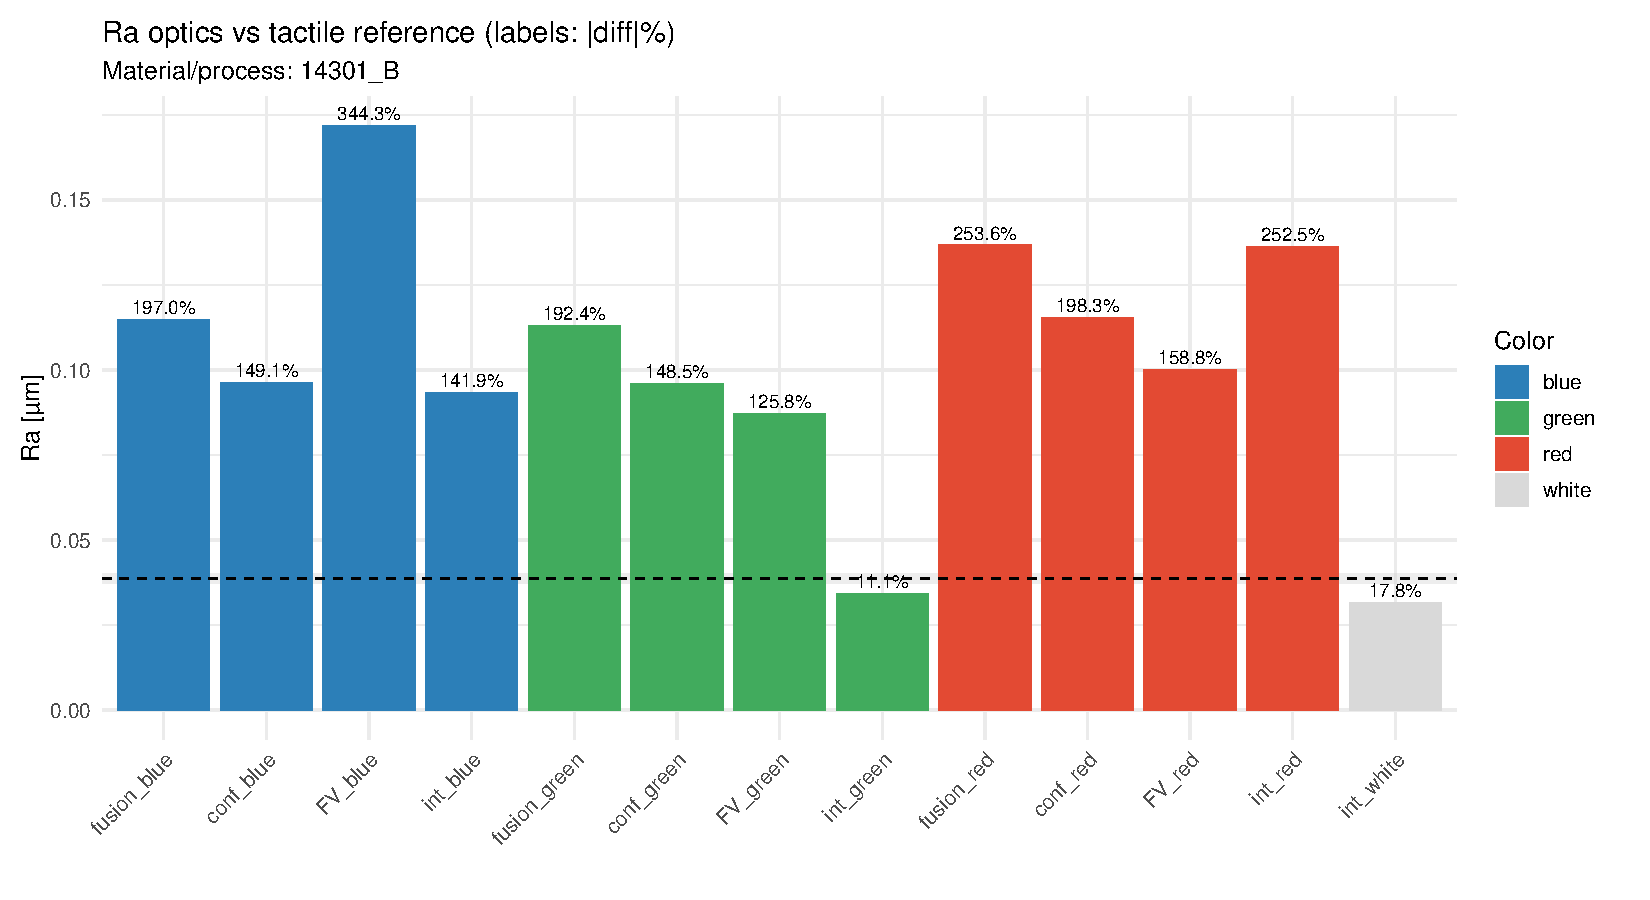
\includegraphics[width=\linewidth]{plots/ra_abs_14301_b_optics_vs_tactile.pdf}
\end{minipage}
\begin{minipage}[t]{0.32\textwidth}\centering
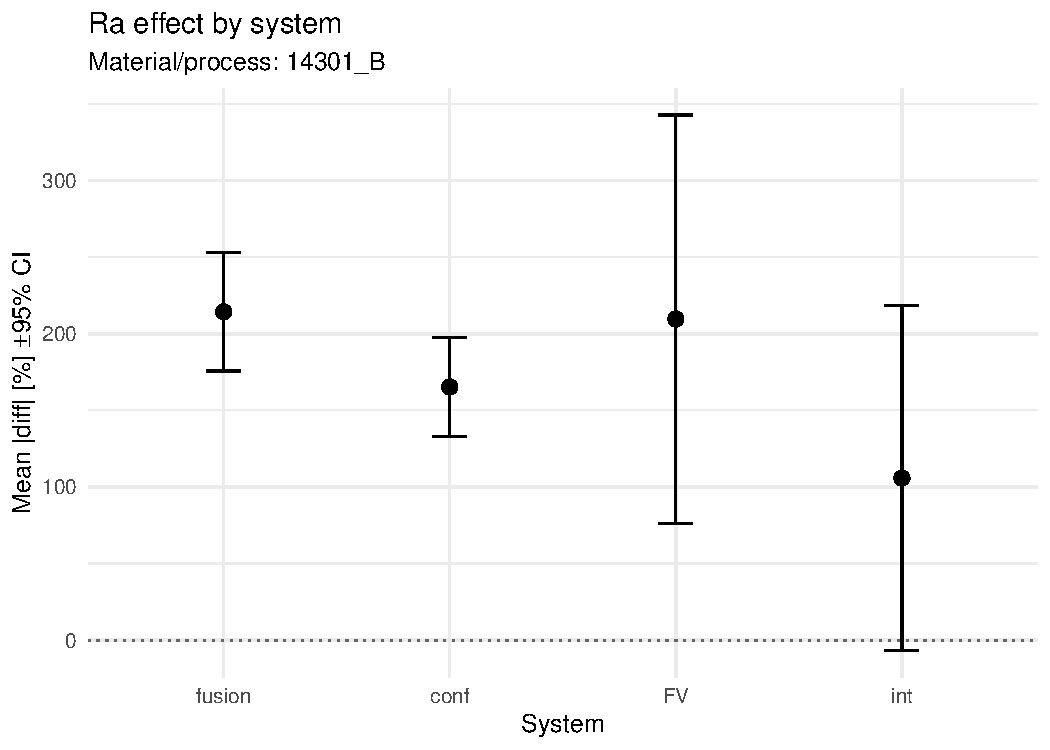
\includegraphics[width=\linewidth]{plots/ra_abs_14301_b_effects_by_system.pdf}
\end{minipage}
\begin{minipage}[t]{0.32\textwidth}\centering
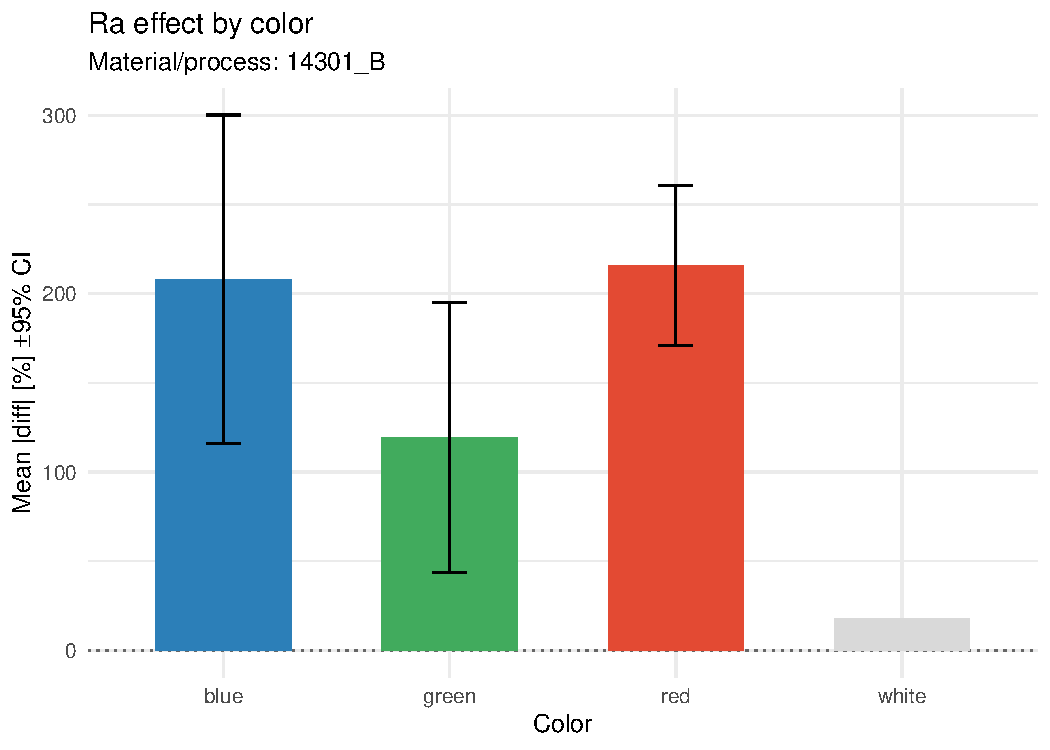
\includegraphics[width=\linewidth]{plots/ra_abs_14301_b_effects_by_color.pdf}
\end{minipage}
\caption{RA — 14301\_b — porównanie i efekty (|diff| \%)}
\end{figure}

\begin{figure}[H]\centering
\begin{minipage}[t]{0.32\textwidth}\centering
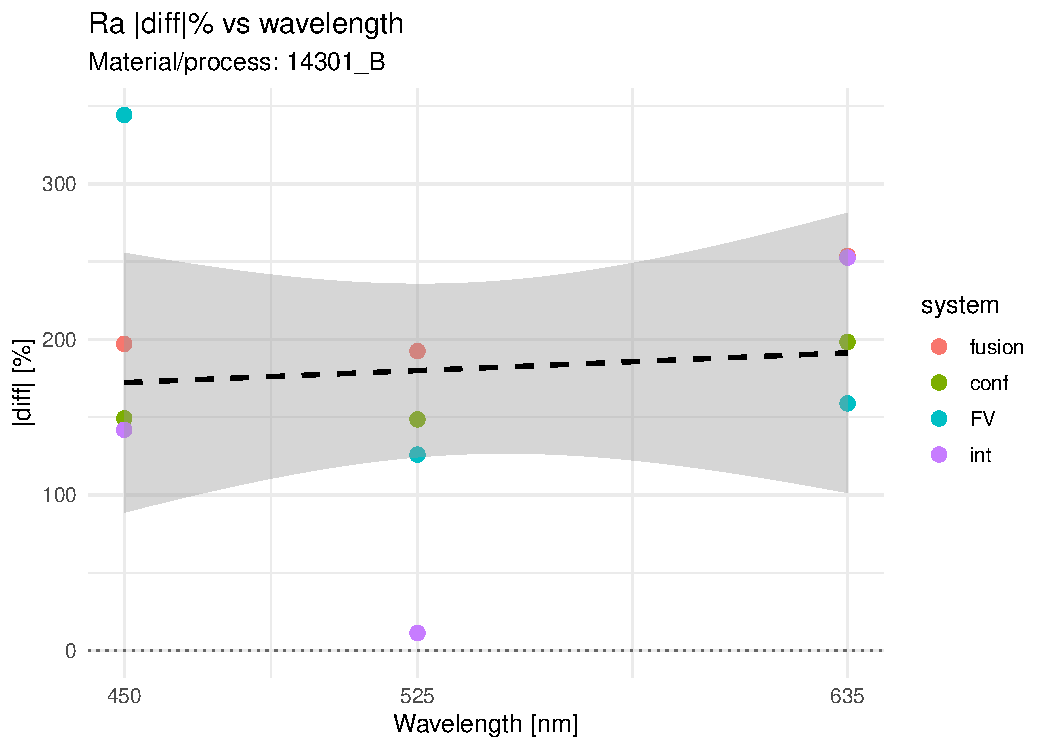
\includegraphics[width=\linewidth]{plots/ra_abs_14301_b_diff_vs_wavelength.pdf}
\end{minipage}
\begin{minipage}[t]{0.32\textwidth}\centering
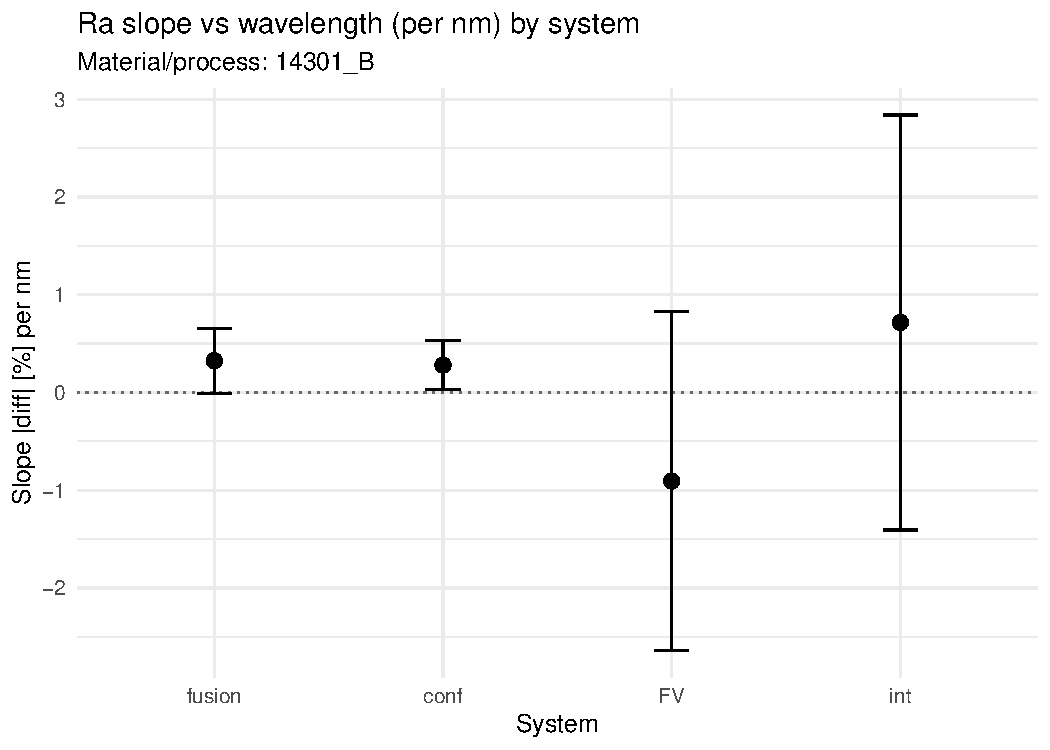
\includegraphics[width=\linewidth]{plots/ra_abs_14301_b_slope_by_system_vs_nm.pdf}
\end{minipage}
\begin{minipage}[t]{0.32\textwidth}\centering
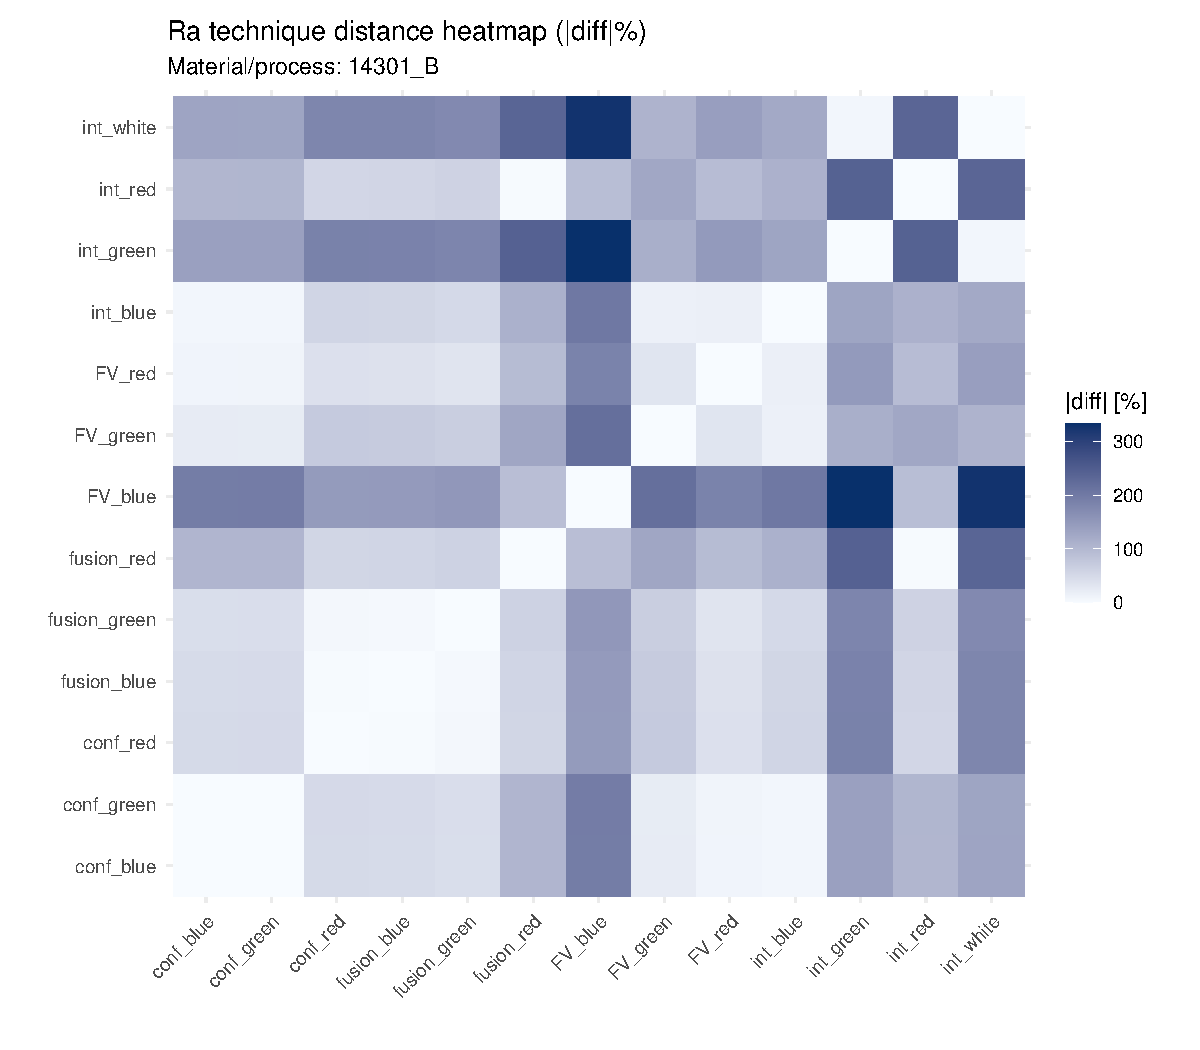
\includegraphics[width=\linewidth]{plots/ra_abs_14301_b_tech_distance_heatmap.pdf}
\end{minipage}
\caption{RA — 14301\_b — wavelength, nachylenia, odległości technik}
\end{figure}

\begin{figure}[H]\centering
\begin{minipage}[t]{0.32\textwidth}\centering
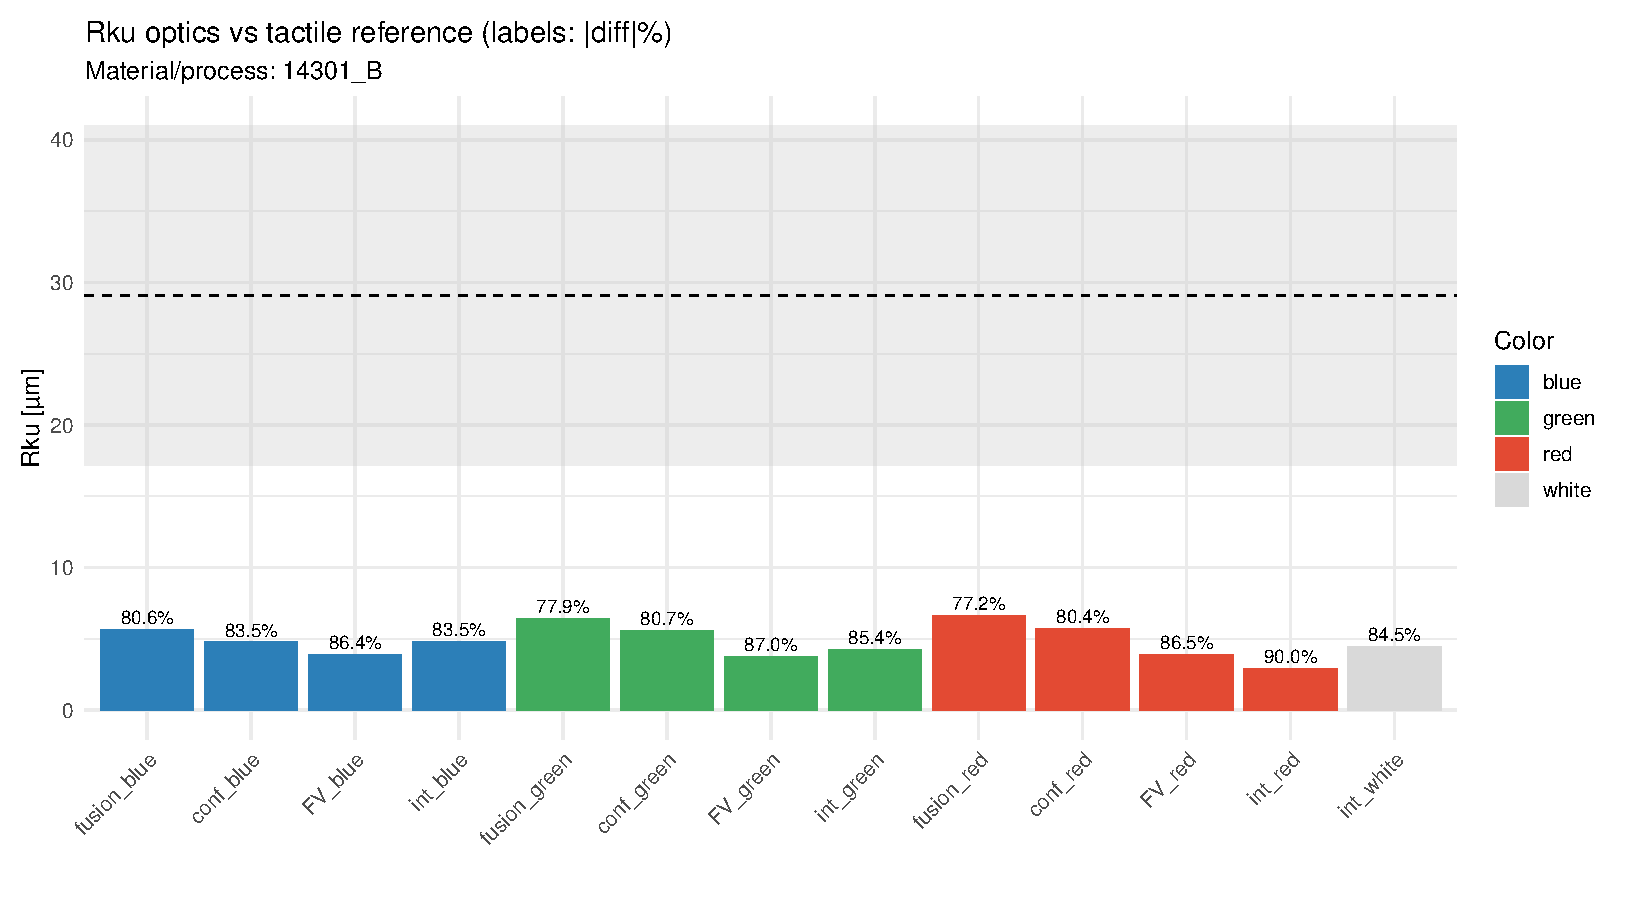
\includegraphics[width=\linewidth]{plots/rku_abs_14301_b_optics_vs_tactile.pdf}
\end{minipage}
\begin{minipage}[t]{0.32\textwidth}\centering
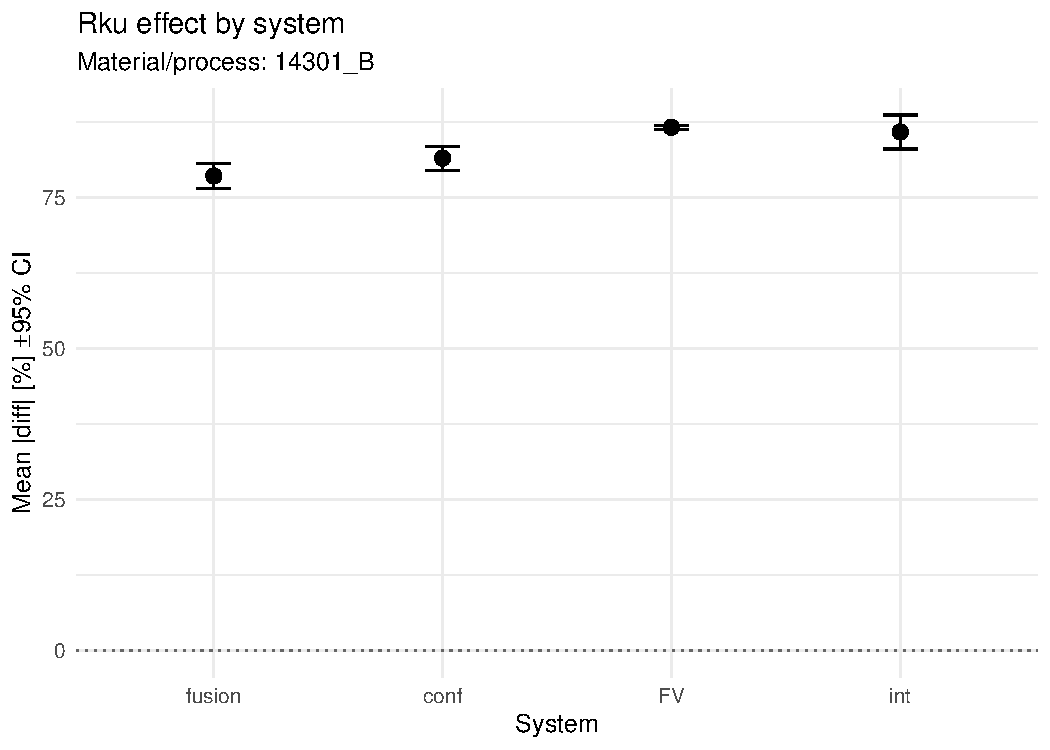
\includegraphics[width=\linewidth]{plots/rku_abs_14301_b_effects_by_system.pdf}
\end{minipage}
\begin{minipage}[t]{0.32\textwidth}\centering
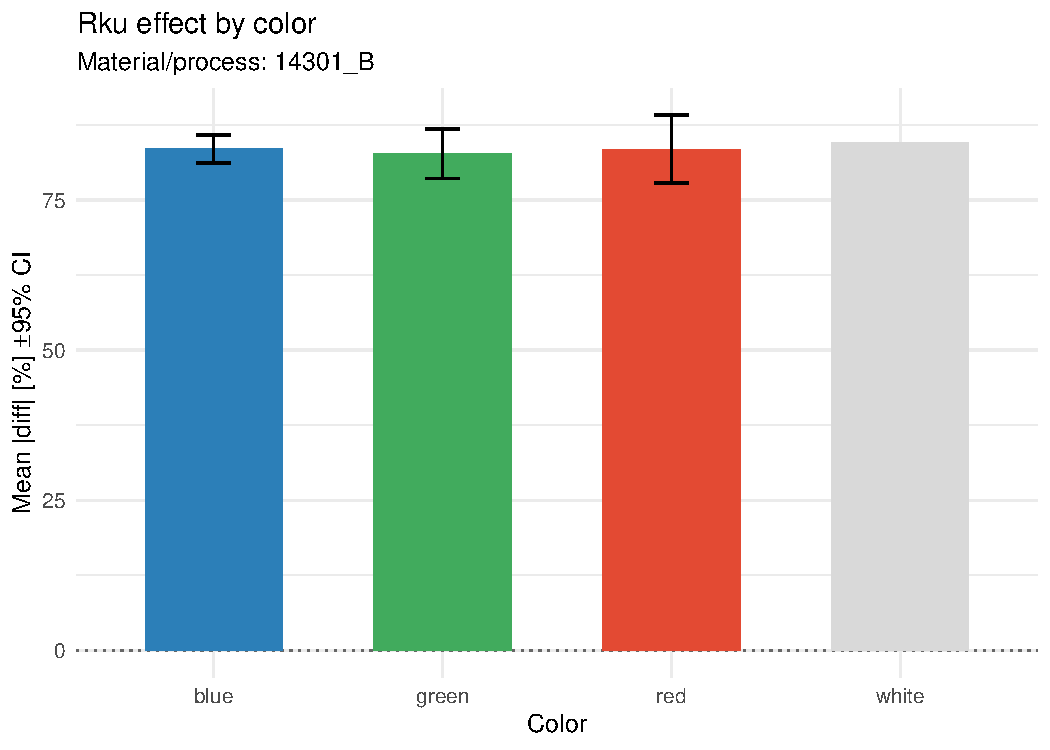
\includegraphics[width=\linewidth]{plots/rku_abs_14301_b_effects_by_color.pdf}
\end{minipage}
\caption{RKU — 14301\_b — porównanie i efekty (|diff| \%)}
\end{figure}

\begin{figure}[H]\centering
\begin{minipage}[t]{0.32\textwidth}\centering
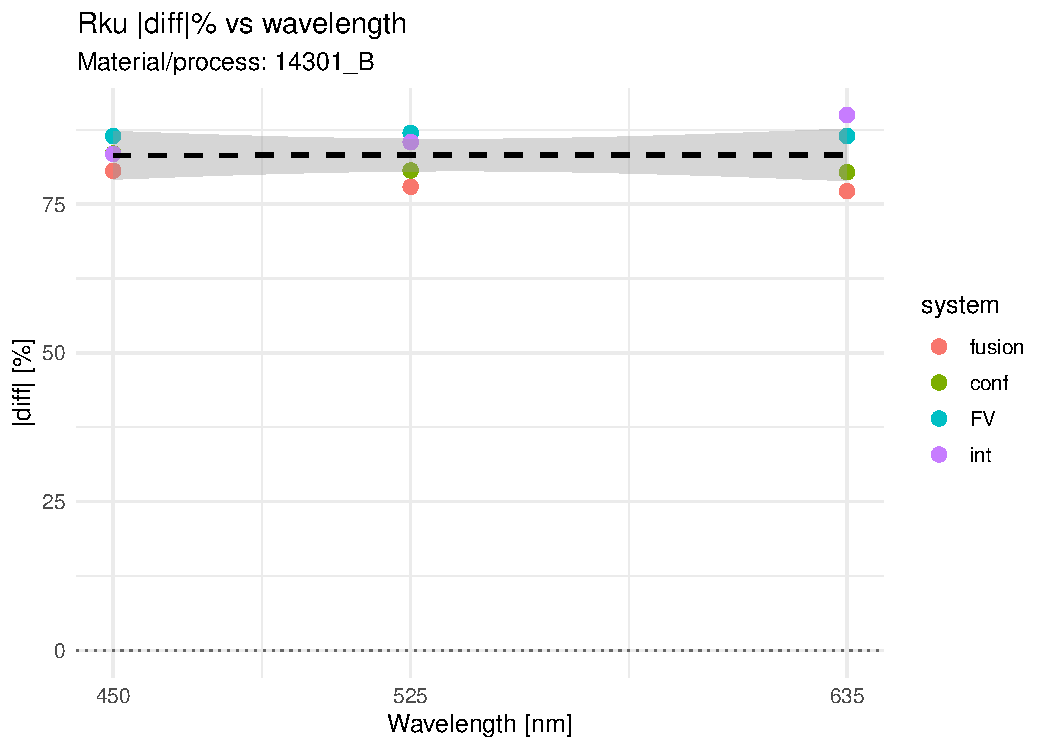
\includegraphics[width=\linewidth]{plots/rku_abs_14301_b_diff_vs_wavelength.pdf}
\end{minipage}
\begin{minipage}[t]{0.32\textwidth}\centering
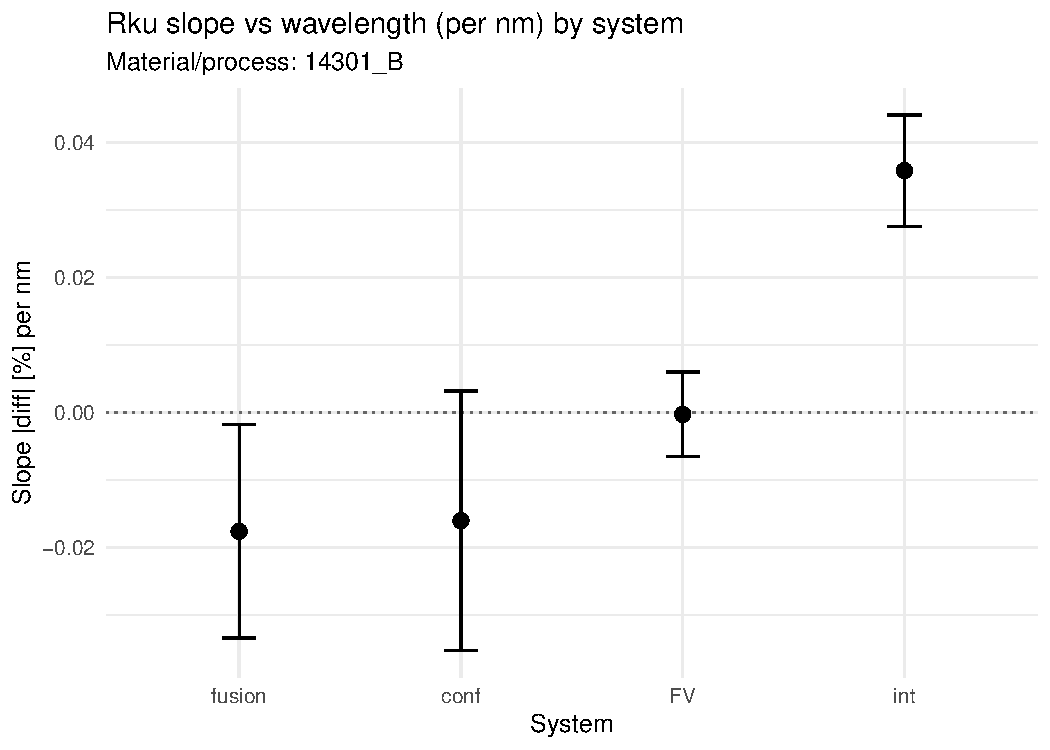
\includegraphics[width=\linewidth]{plots/rku_abs_14301_b_slope_by_system_vs_nm.pdf}
\end{minipage}
\begin{minipage}[t]{0.32\textwidth}\centering
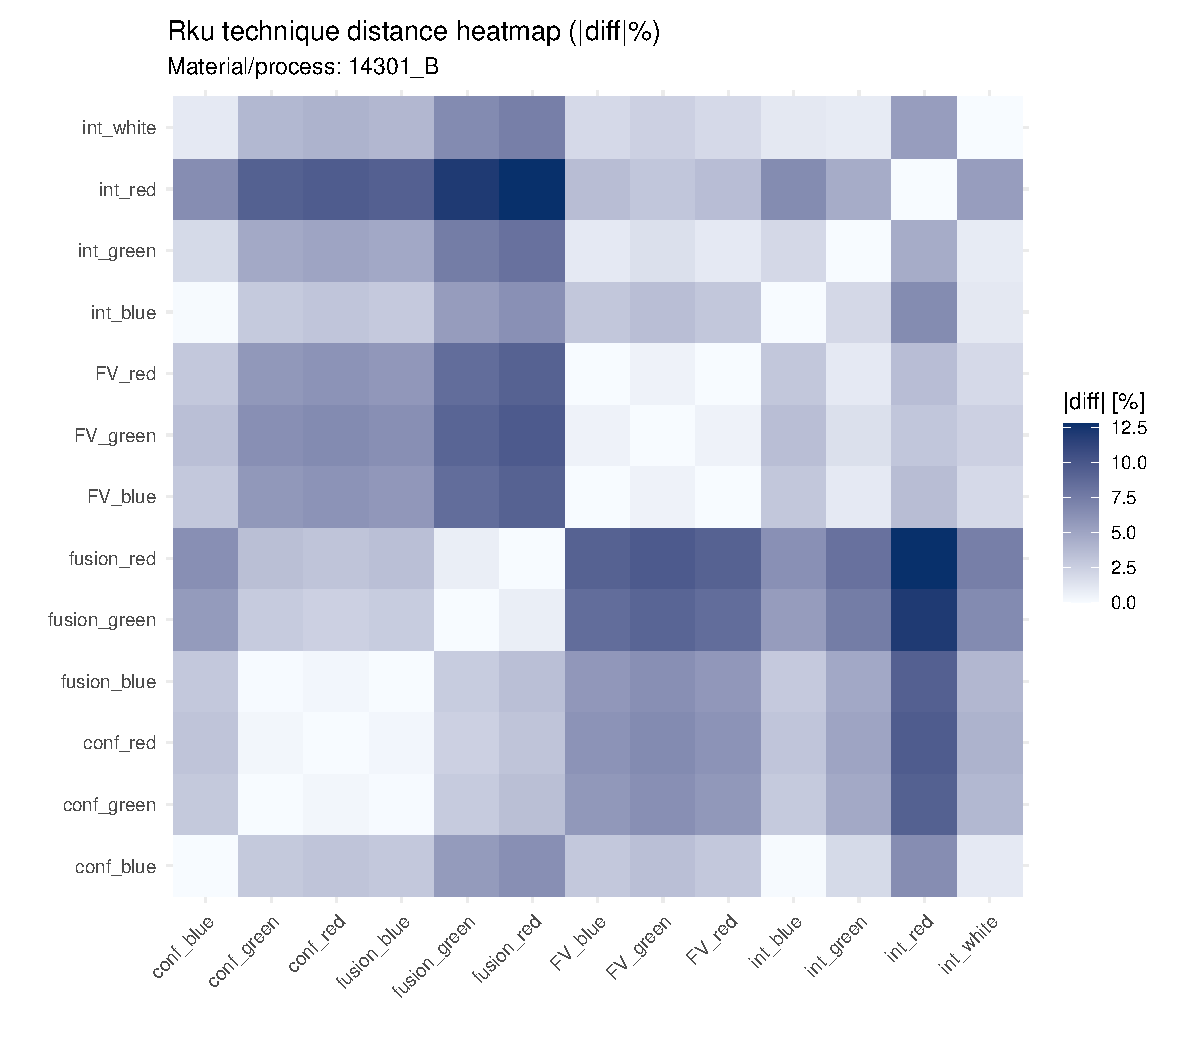
\includegraphics[width=\linewidth]{plots/rku_abs_14301_b_tech_distance_heatmap.pdf}
\end{minipage}
\caption{RKU — 14301\_b — wavelength, nachylenia, odległości technik}
\end{figure}

\begin{figure}[H]\centering
\begin{minipage}[t]{0.32\textwidth}\centering
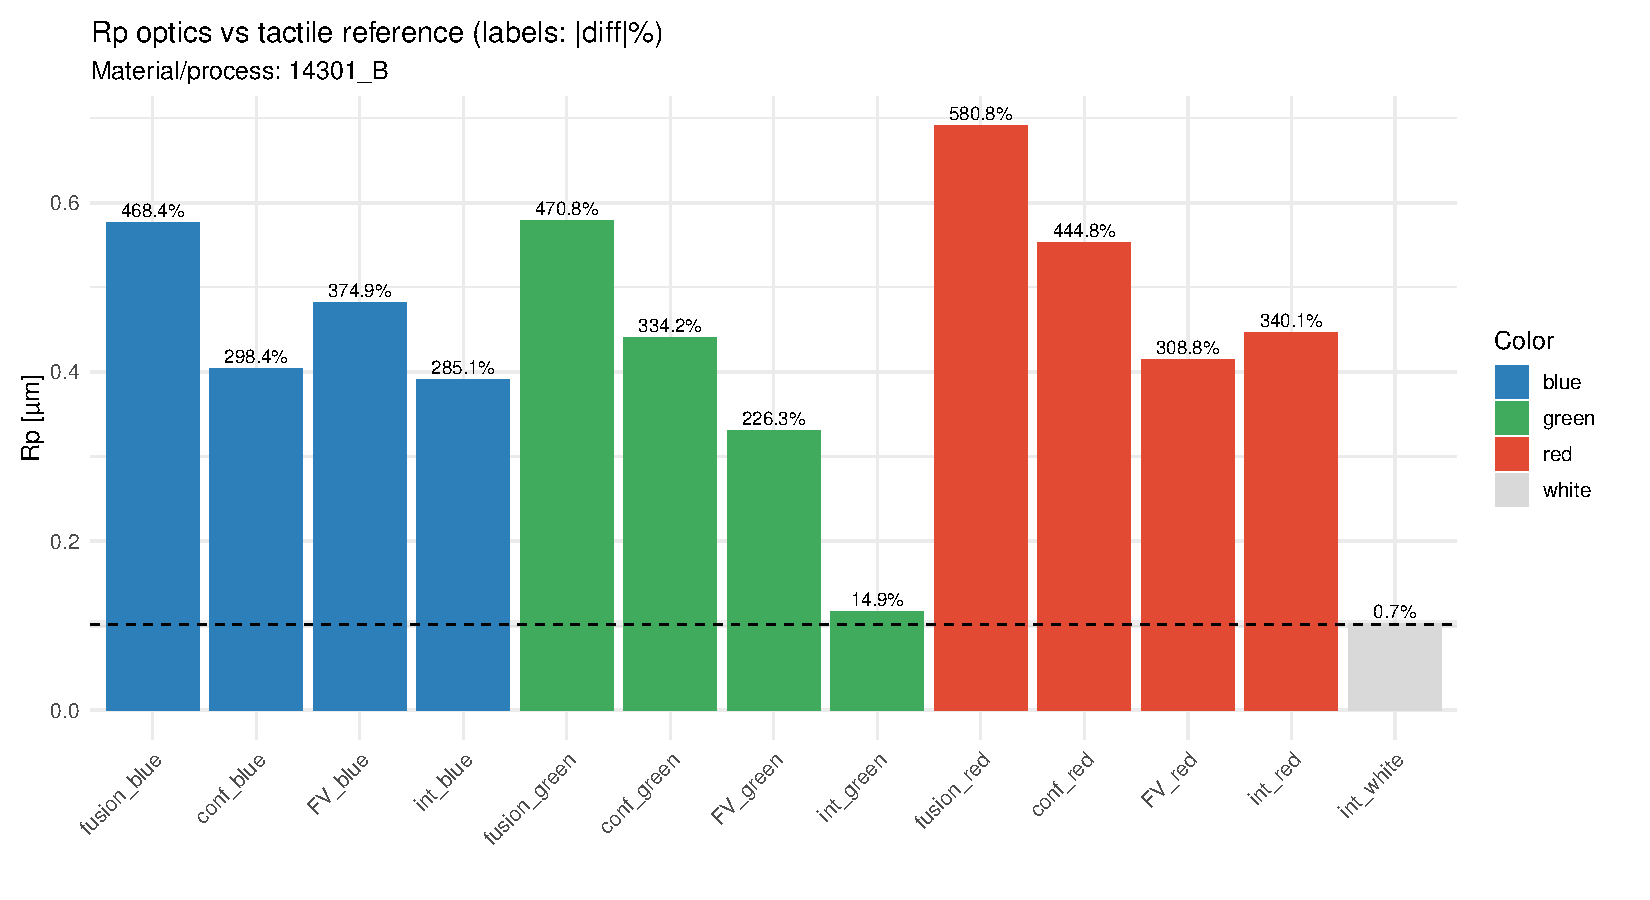
\includegraphics[width=\linewidth]{plots/rp_abs_14301_b_optics_vs_tactile.pdf}
\end{minipage}
\begin{minipage}[t]{0.32\textwidth}\centering
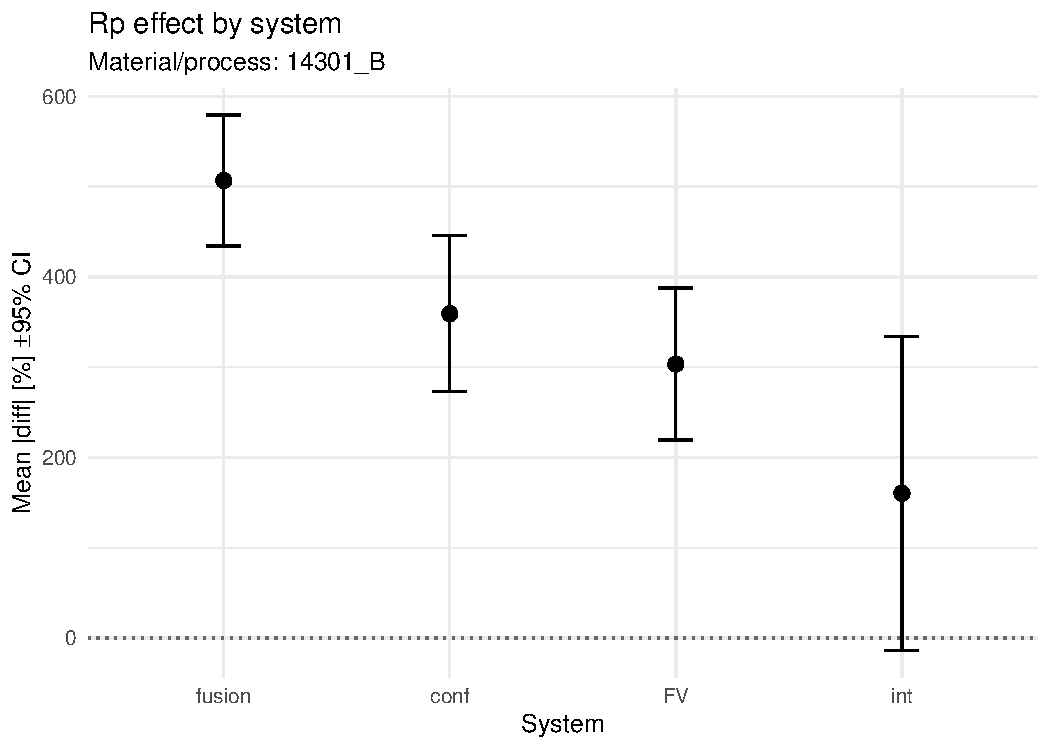
\includegraphics[width=\linewidth]{plots/rp_abs_14301_b_effects_by_system.pdf}
\end{minipage}
\begin{minipage}[t]{0.32\textwidth}\centering
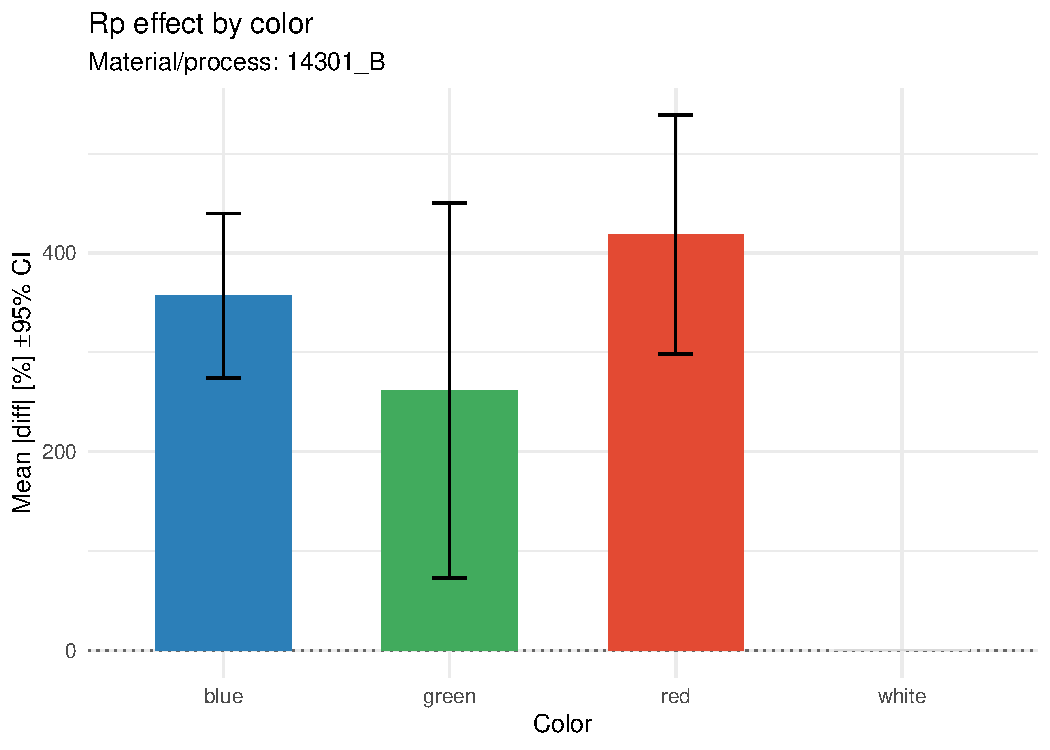
\includegraphics[width=\linewidth]{plots/rp_abs_14301_b_effects_by_color.pdf}
\end{minipage}
\caption{RP — 14301\_b — porównanie i efekty (|diff| \%)}
\end{figure}

\begin{figure}[H]\centering
\begin{minipage}[t]{0.32\textwidth}\centering
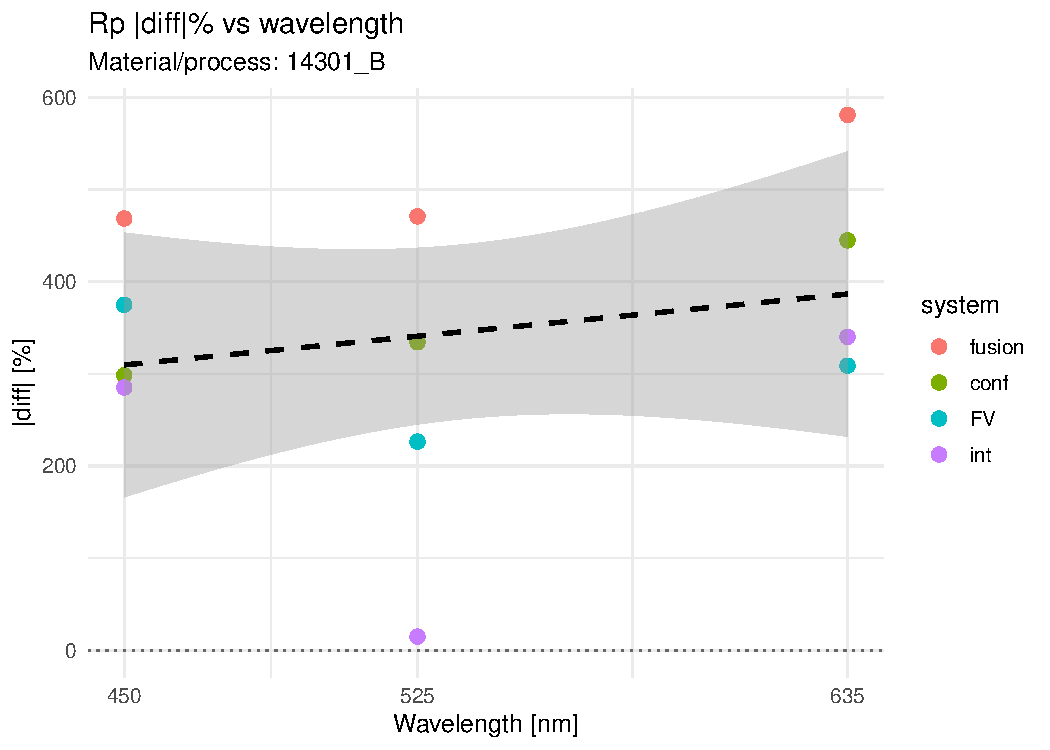
\includegraphics[width=\linewidth]{plots/rp_abs_14301_b_diff_vs_wavelength.pdf}
\end{minipage}
\begin{minipage}[t]{0.32\textwidth}\centering
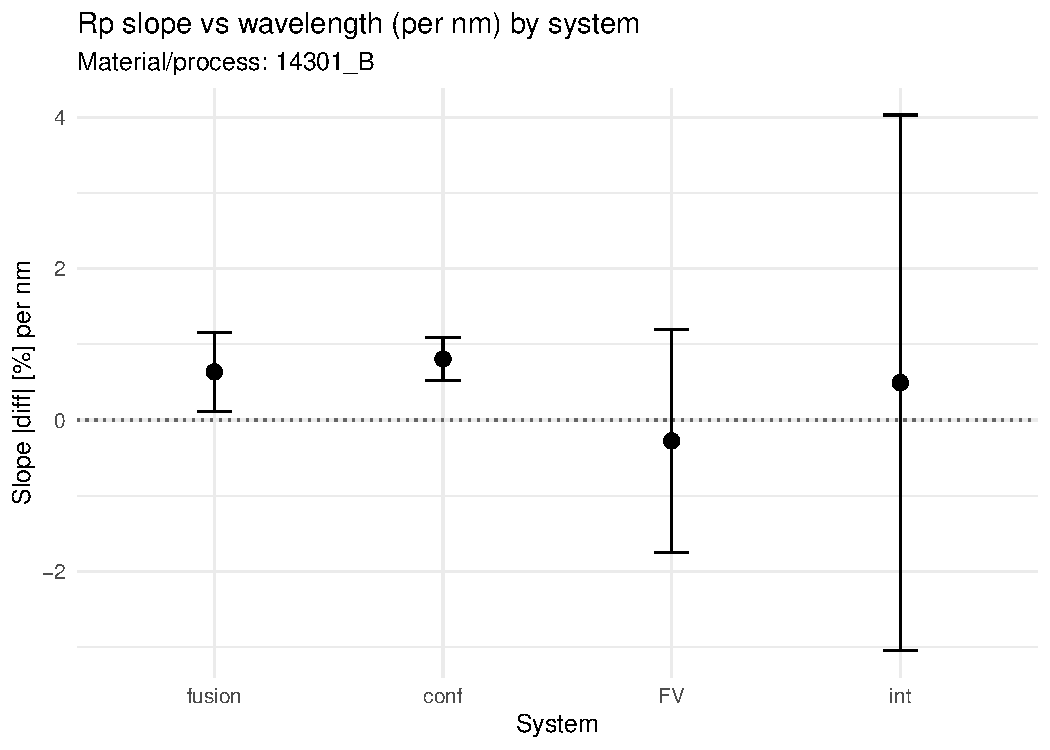
\includegraphics[width=\linewidth]{plots/rp_abs_14301_b_slope_by_system_vs_nm.pdf}
\end{minipage}
\begin{minipage}[t]{0.32\textwidth}\centering
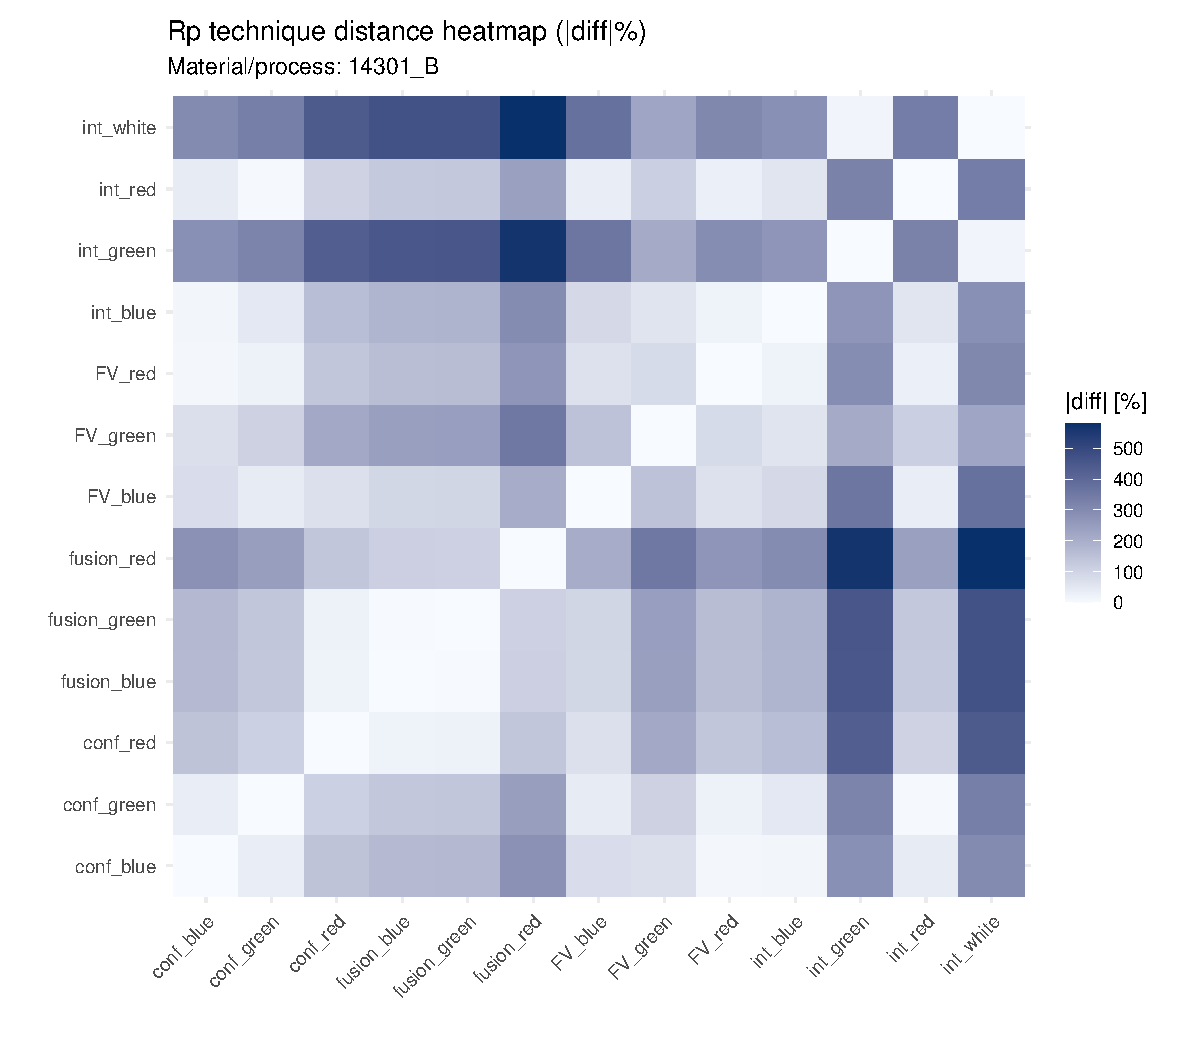
\includegraphics[width=\linewidth]{plots/rp_abs_14301_b_tech_distance_heatmap.pdf}
\end{minipage}
\caption{RP — 14301\_b — wavelength, nachylenia, odległości technik}
\end{figure}

\begin{figure}[H]\centering
\begin{minipage}[t]{0.32\textwidth}\centering
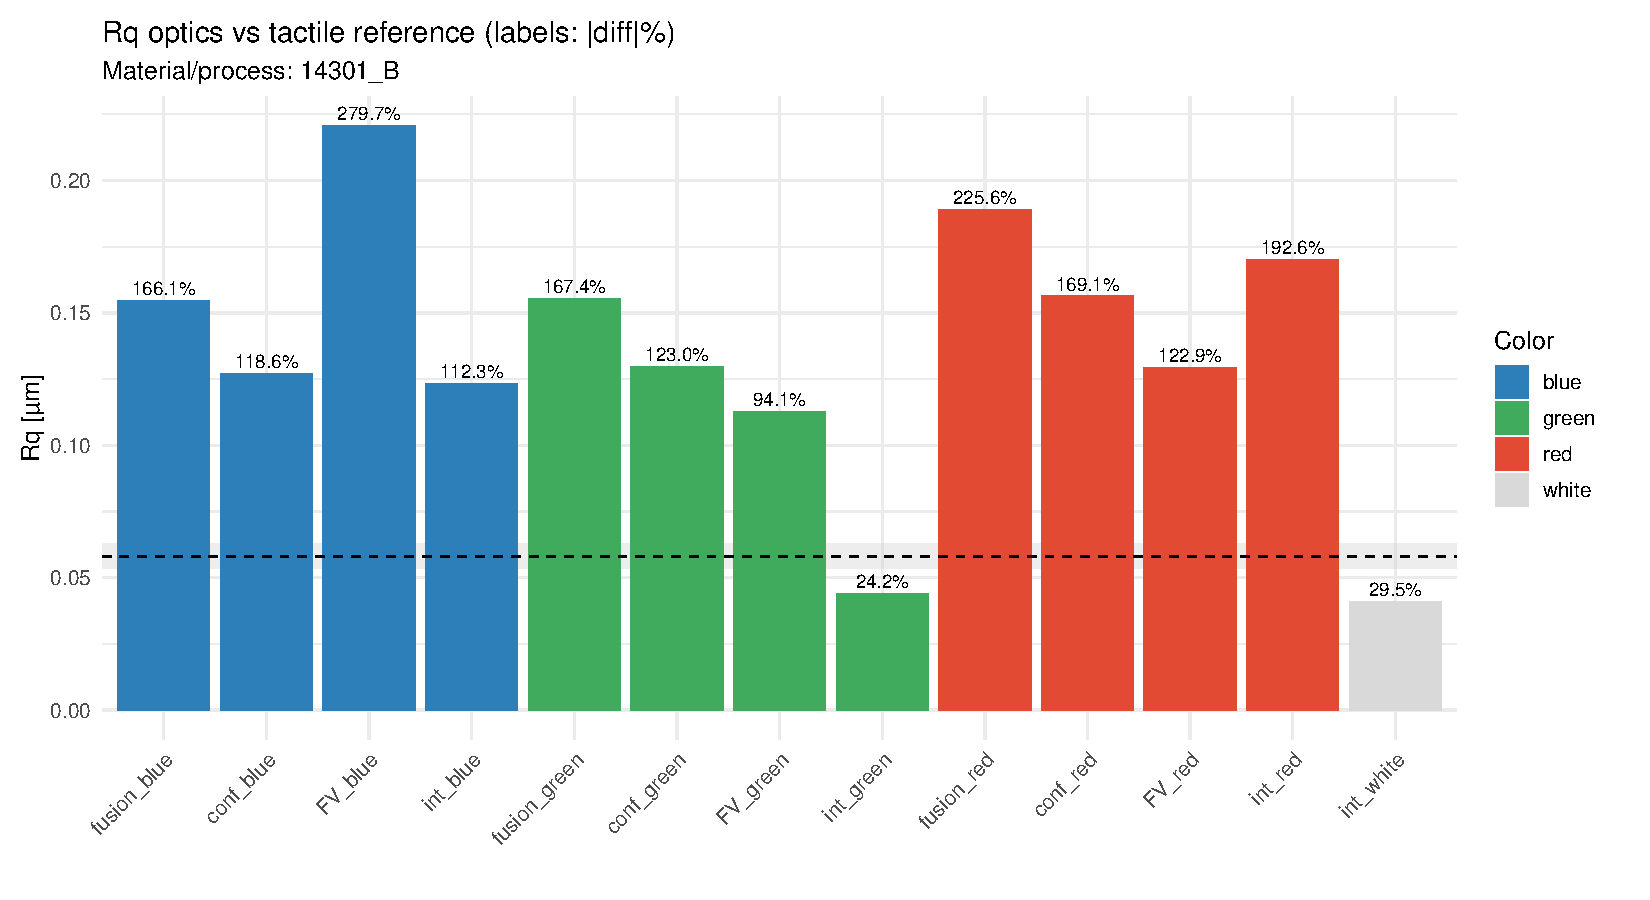
\includegraphics[width=\linewidth]{plots/rq_abs_14301_b_optics_vs_tactile.pdf}
\end{minipage}
\begin{minipage}[t]{0.32\textwidth}\centering
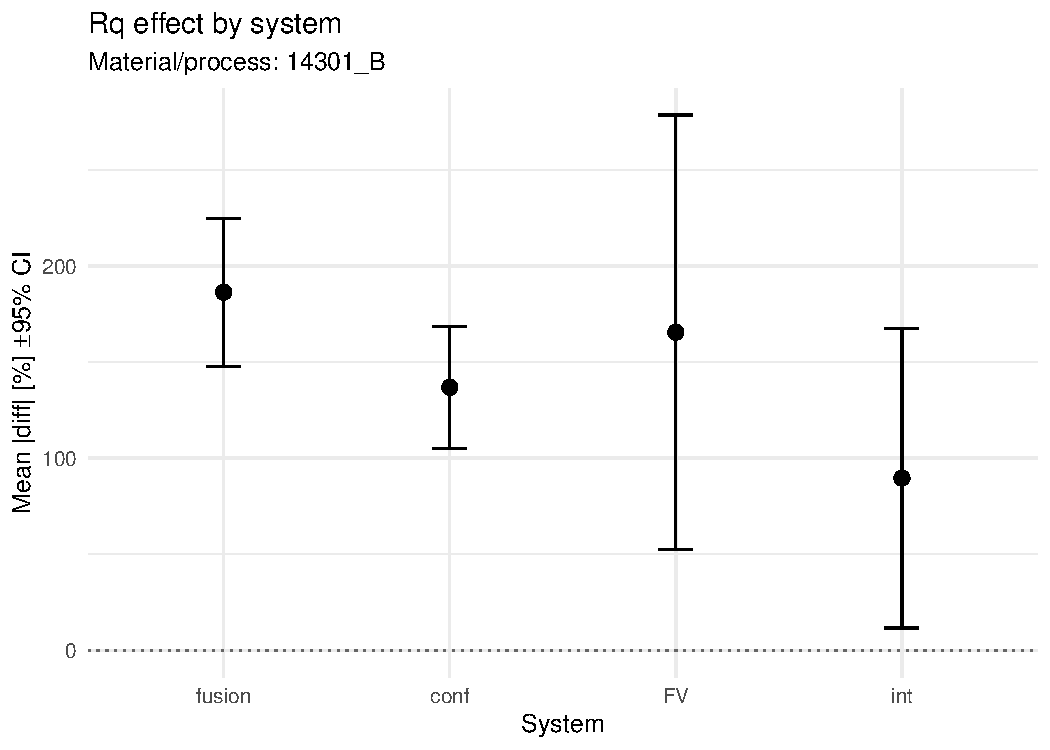
\includegraphics[width=\linewidth]{plots/rq_abs_14301_b_effects_by_system.pdf}
\end{minipage}
\begin{minipage}[t]{0.32\textwidth}\centering
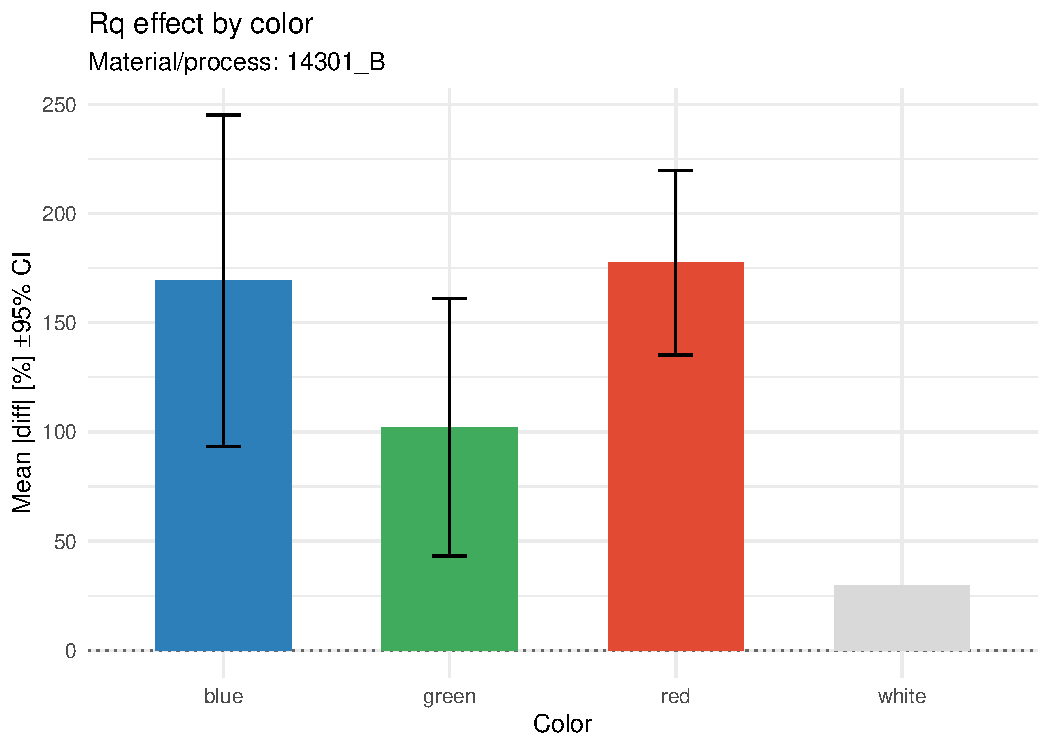
\includegraphics[width=\linewidth]{plots/rq_abs_14301_b_effects_by_color.pdf}
\end{minipage}
\caption{RQ — 14301\_b — porównanie i efekty (|diff| \%)}
\end{figure}

\begin{figure}[H]\centering
\begin{minipage}[t]{0.32\textwidth}\centering
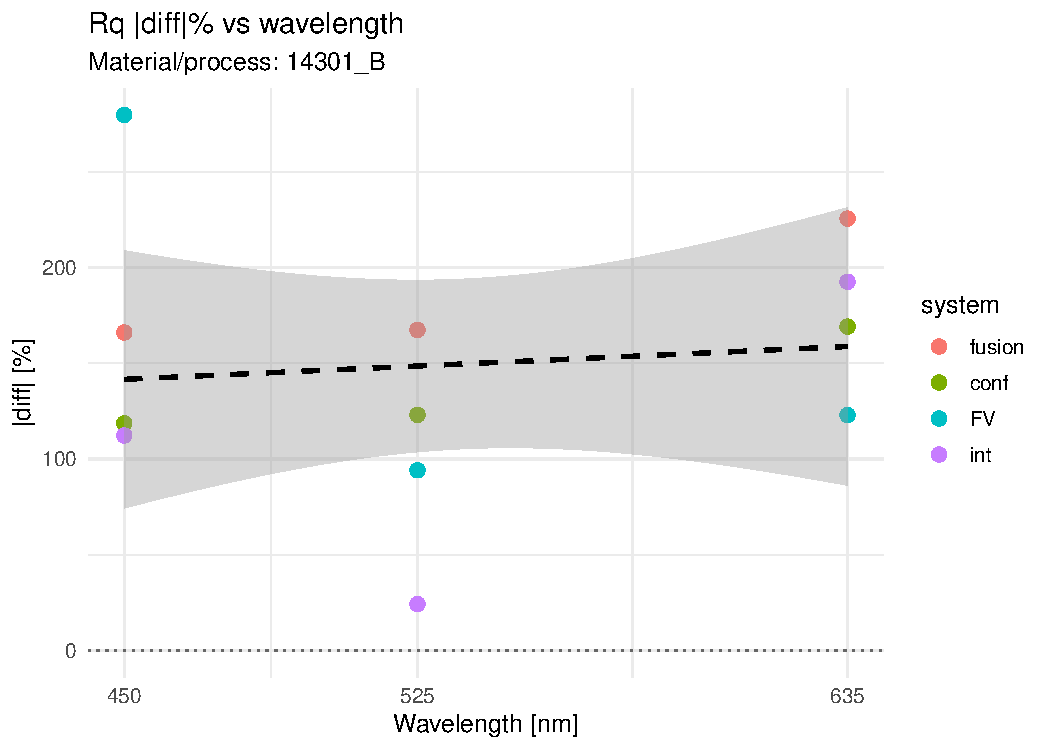
\includegraphics[width=\linewidth]{plots/rq_abs_14301_b_diff_vs_wavelength.pdf}
\end{minipage}
\begin{minipage}[t]{0.32\textwidth}\centering
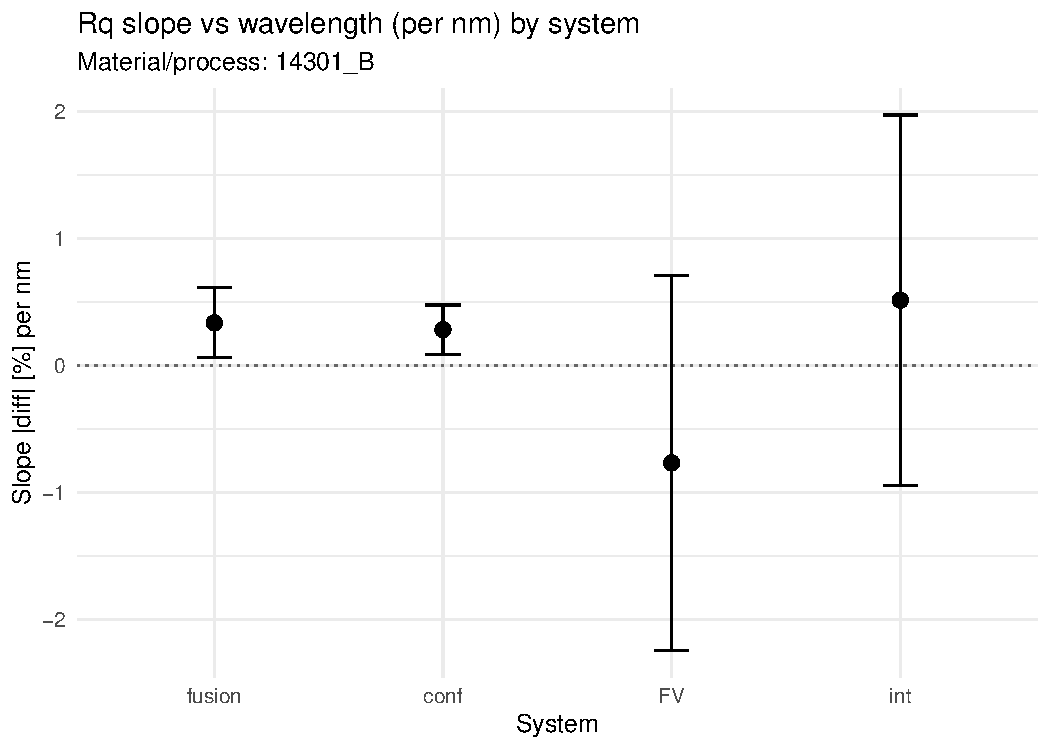
\includegraphics[width=\linewidth]{plots/rq_abs_14301_b_slope_by_system_vs_nm.pdf}
\end{minipage}
\begin{minipage}[t]{0.32\textwidth}\centering
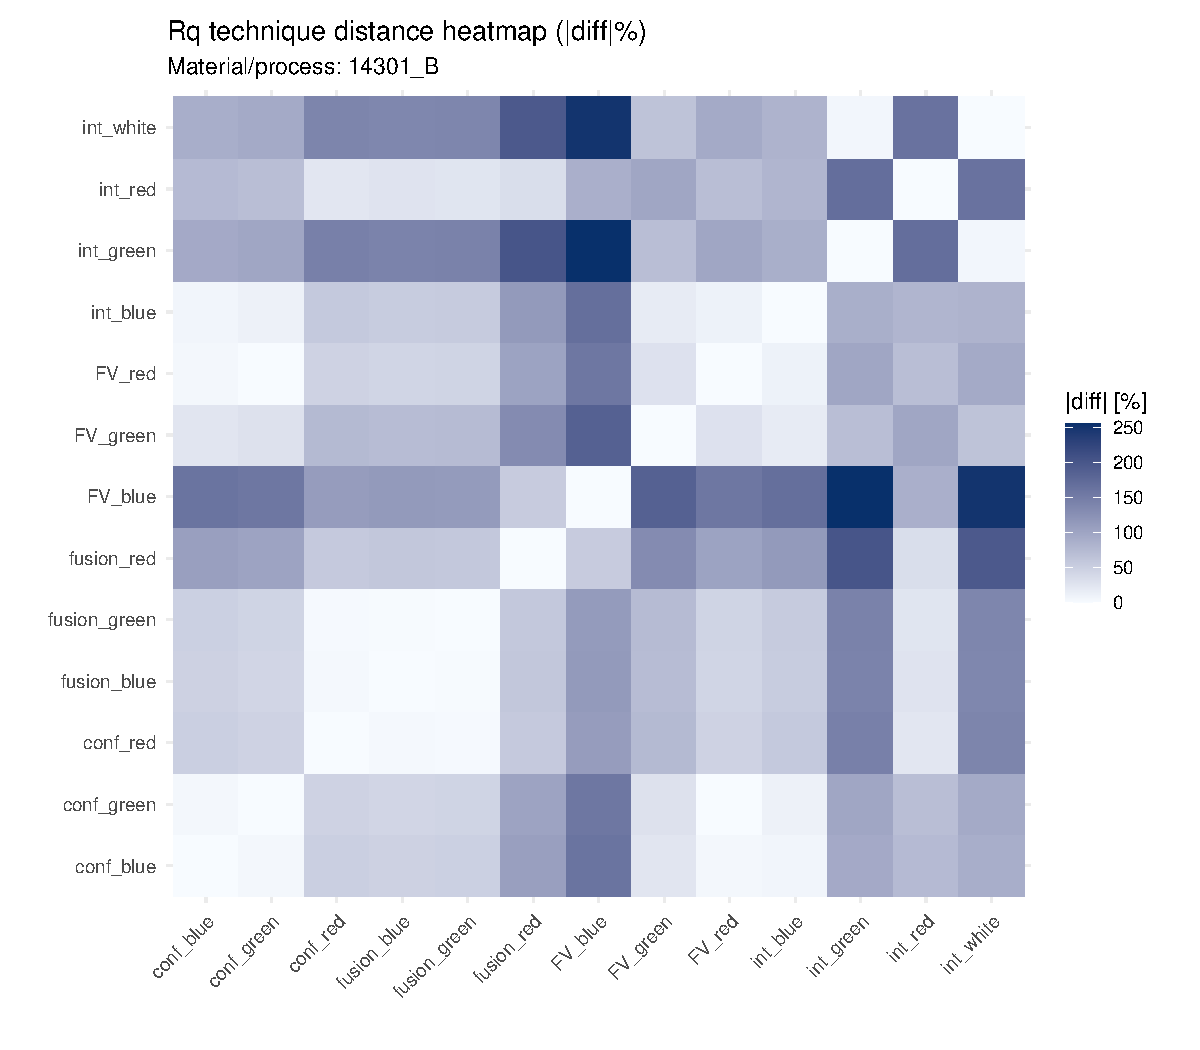
\includegraphics[width=\linewidth]{plots/rq_abs_14301_b_tech_distance_heatmap.pdf}
\end{minipage}
\caption{RQ — 14301\_b — wavelength, nachylenia, odległości technik}
\end{figure}

\begin{figure}[H]\centering
\begin{minipage}[t]{0.32\textwidth}\centering
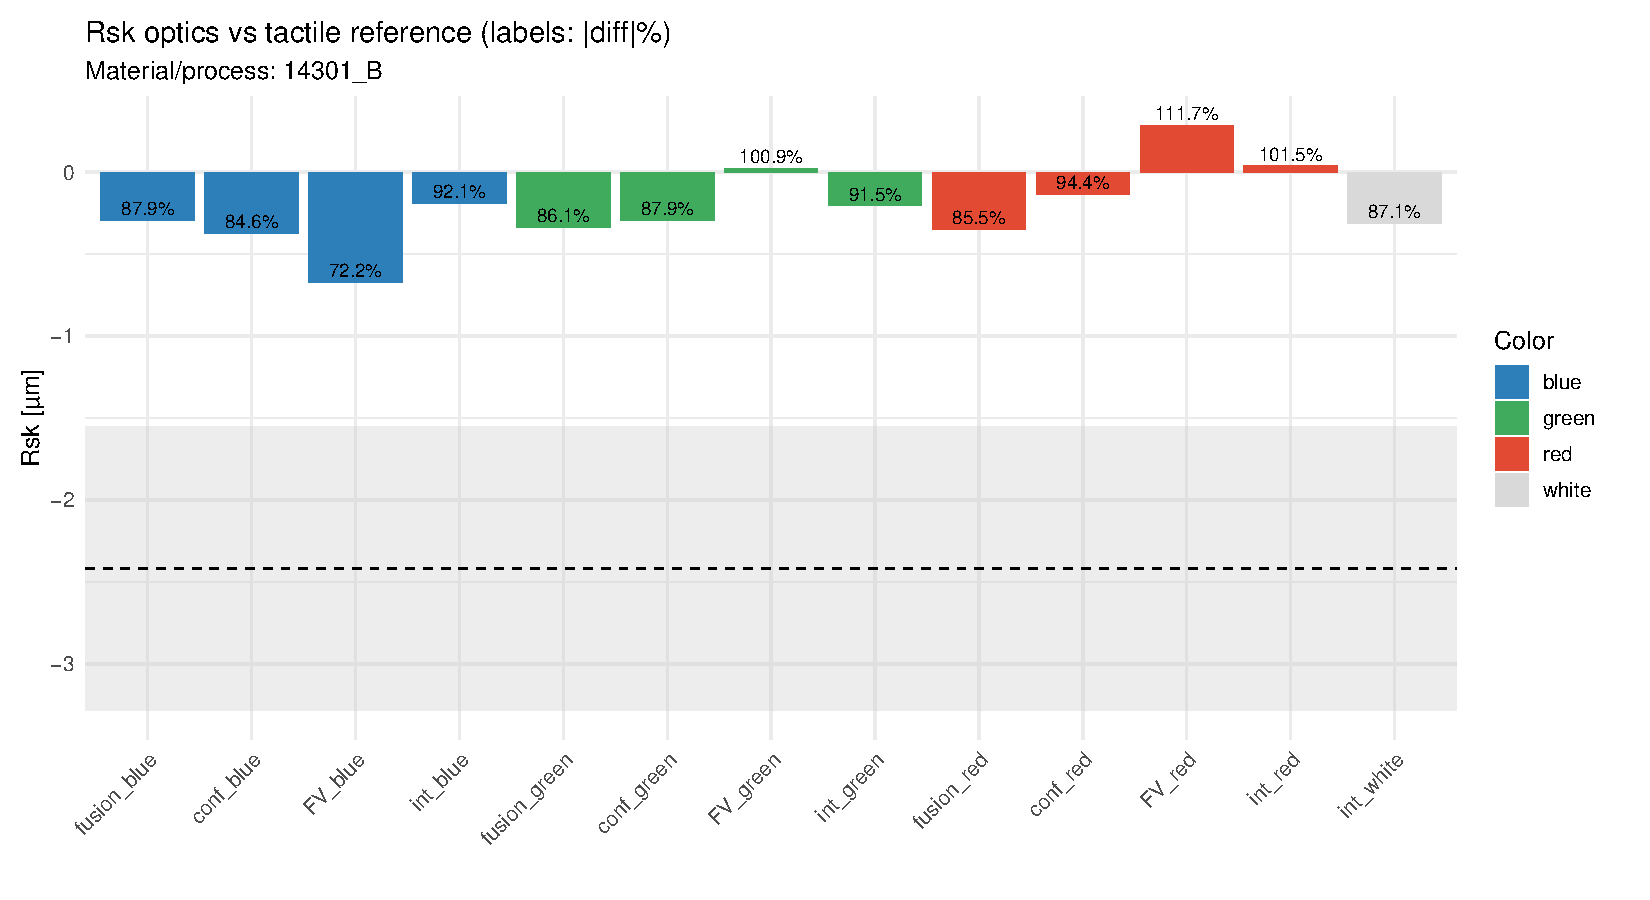
\includegraphics[width=\linewidth]{plots/rsk_abs_14301_b_optics_vs_tactile.pdf}
\end{minipage}
\begin{minipage}[t]{0.32\textwidth}\centering
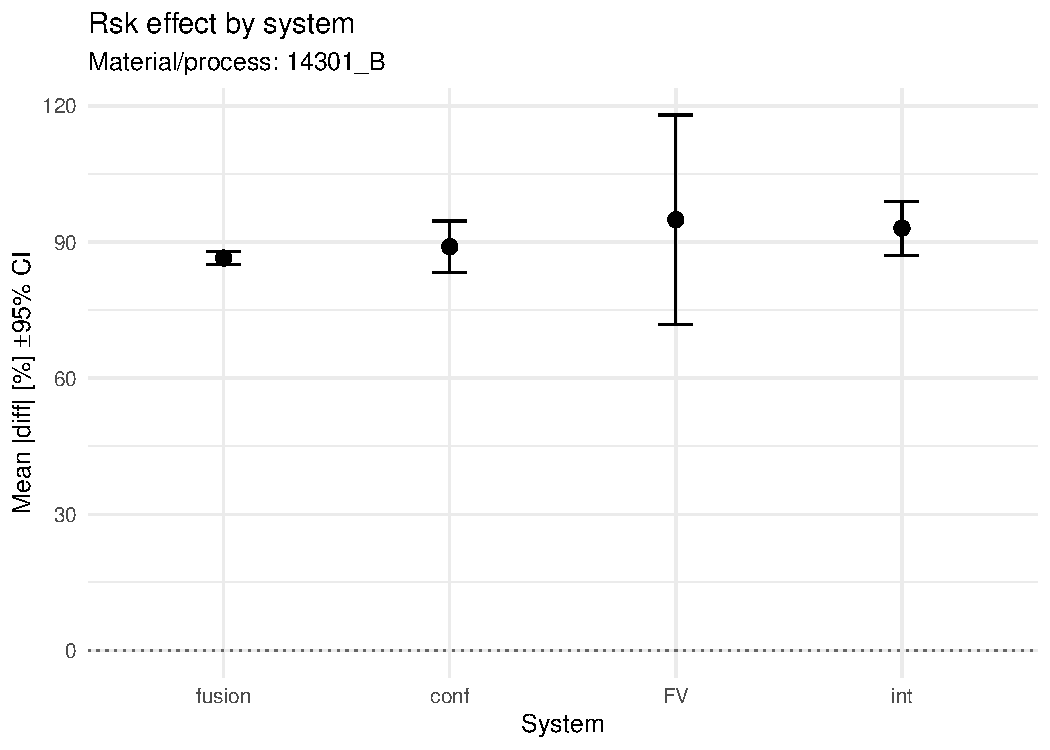
\includegraphics[width=\linewidth]{plots/rsk_abs_14301_b_effects_by_system.pdf}
\end{minipage}
\begin{minipage}[t]{0.32\textwidth}\centering
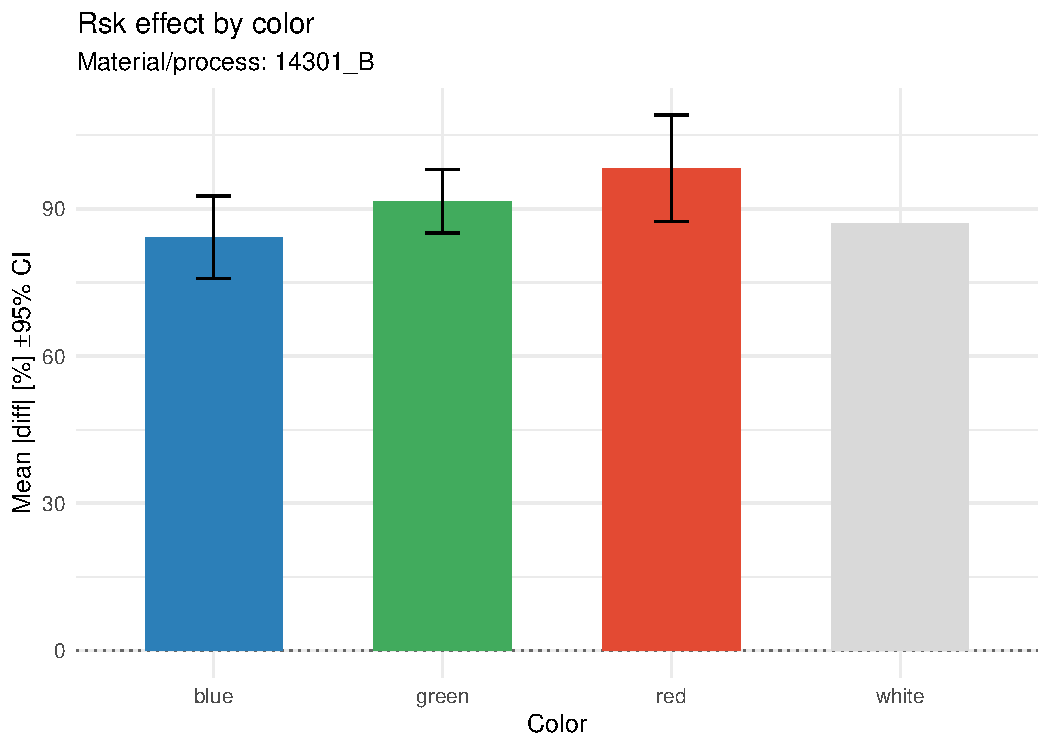
\includegraphics[width=\linewidth]{plots/rsk_abs_14301_b_effects_by_color.pdf}
\end{minipage}
\caption{RSK — 14301\_b — porównanie i efekty (|diff| \%)}
\end{figure}

\begin{figure}[H]\centering
\begin{minipage}[t]{0.32\textwidth}\centering
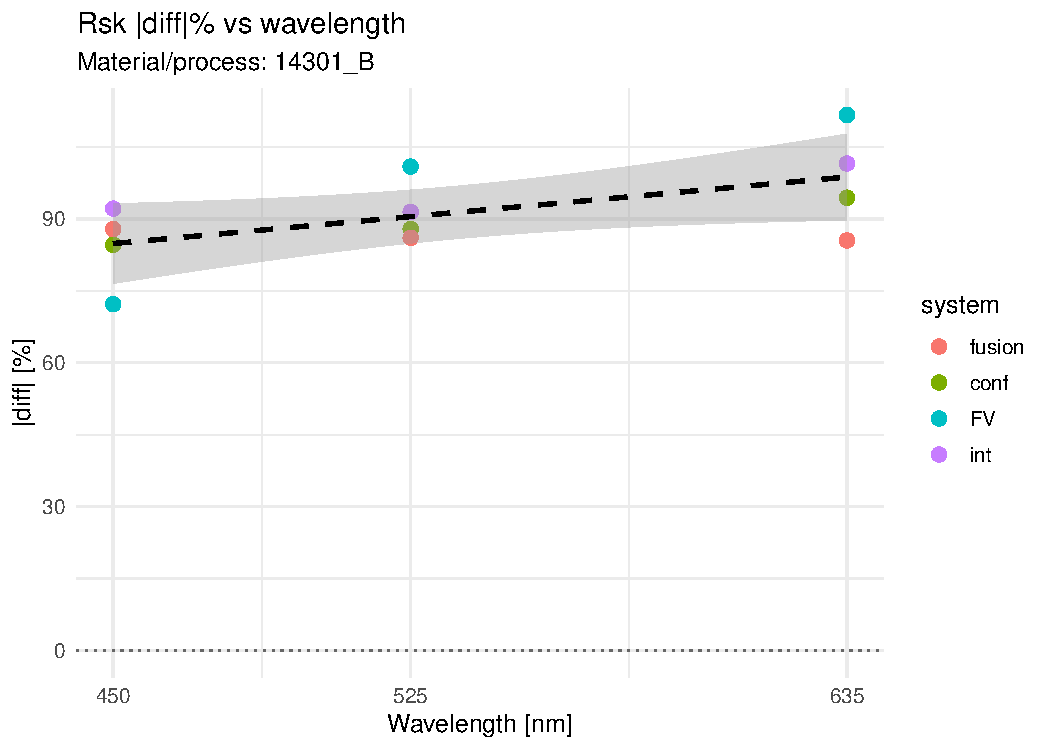
\includegraphics[width=\linewidth]{plots/rsk_abs_14301_b_diff_vs_wavelength.pdf}
\end{minipage}
\begin{minipage}[t]{0.32\textwidth}\centering
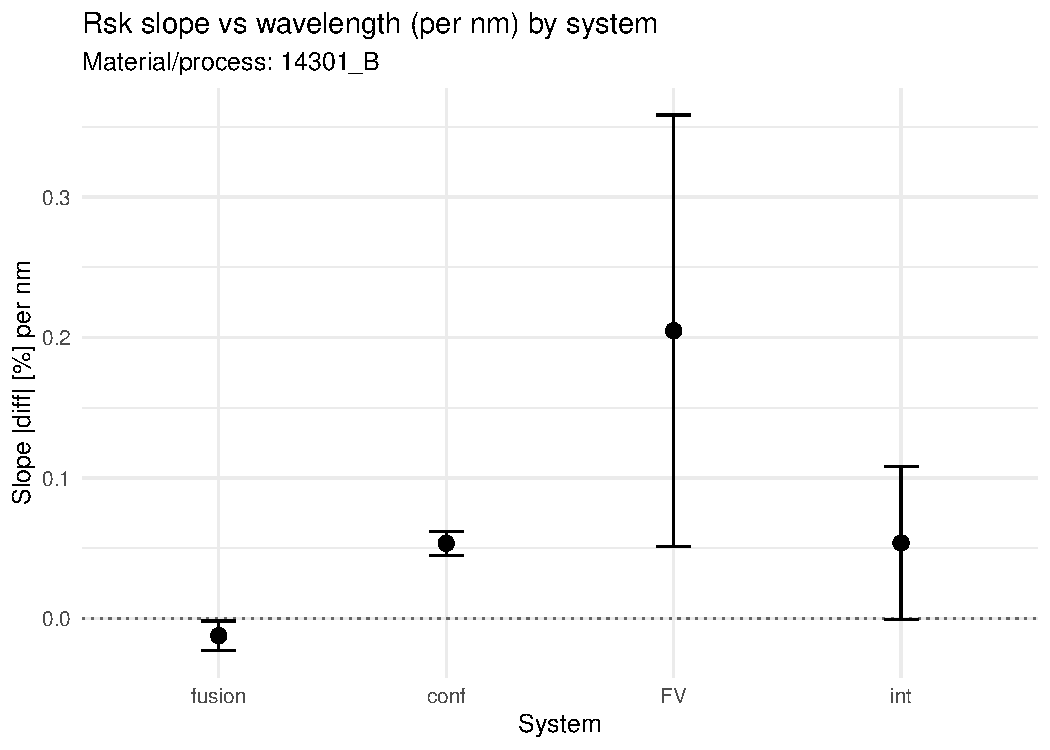
\includegraphics[width=\linewidth]{plots/rsk_abs_14301_b_slope_by_system_vs_nm.pdf}
\end{minipage}
\begin{minipage}[t]{0.32\textwidth}\centering
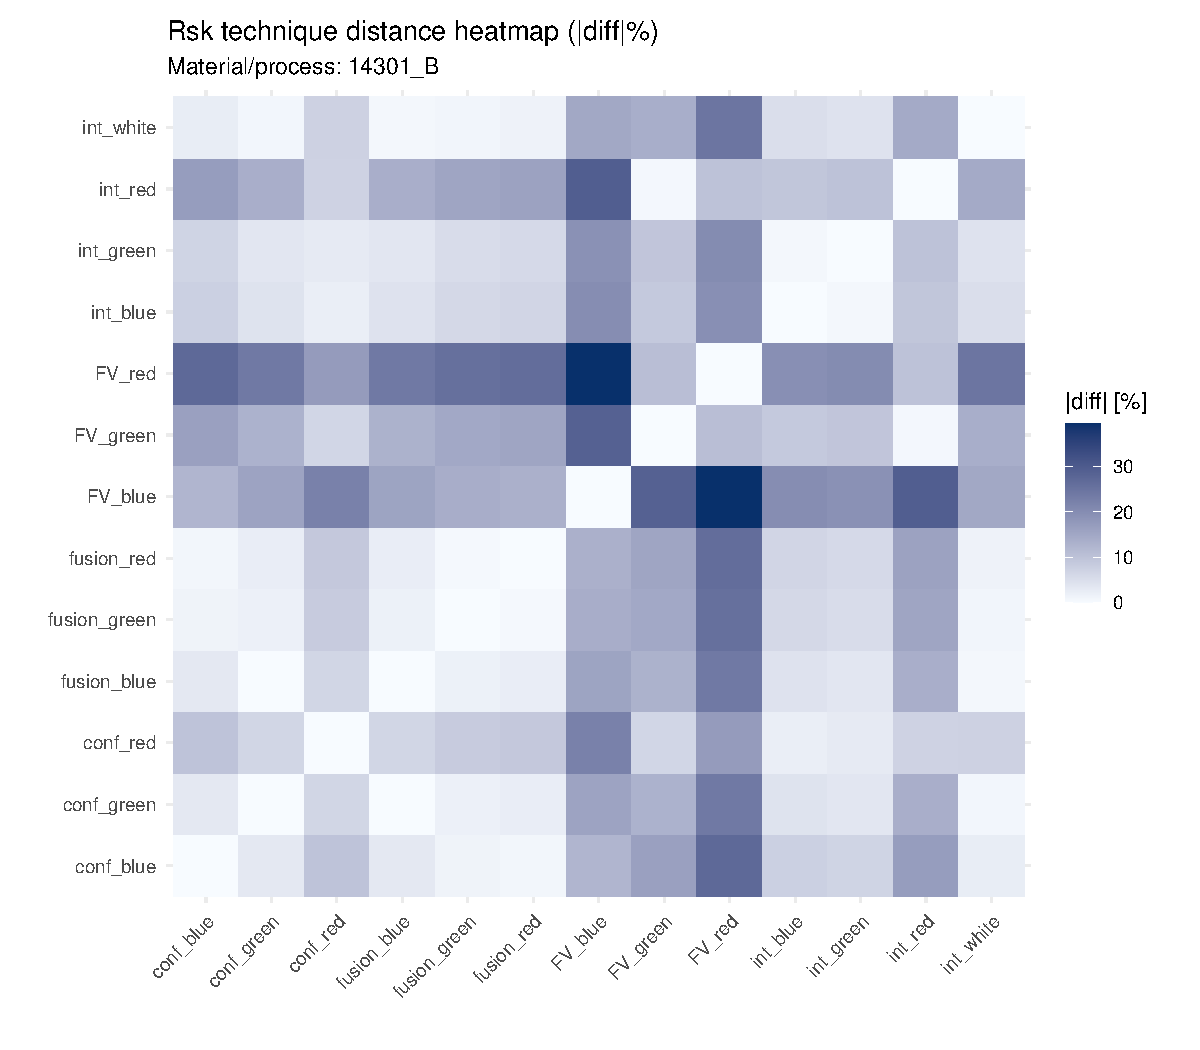
\includegraphics[width=\linewidth]{plots/rsk_abs_14301_b_tech_distance_heatmap.pdf}
\end{minipage}
\caption{RSK — 14301\_b — wavelength, nachylenia, odległości technik}
\end{figure}

\begin{figure}[H]\centering
\begin{minipage}[t]{0.32\textwidth}\centering
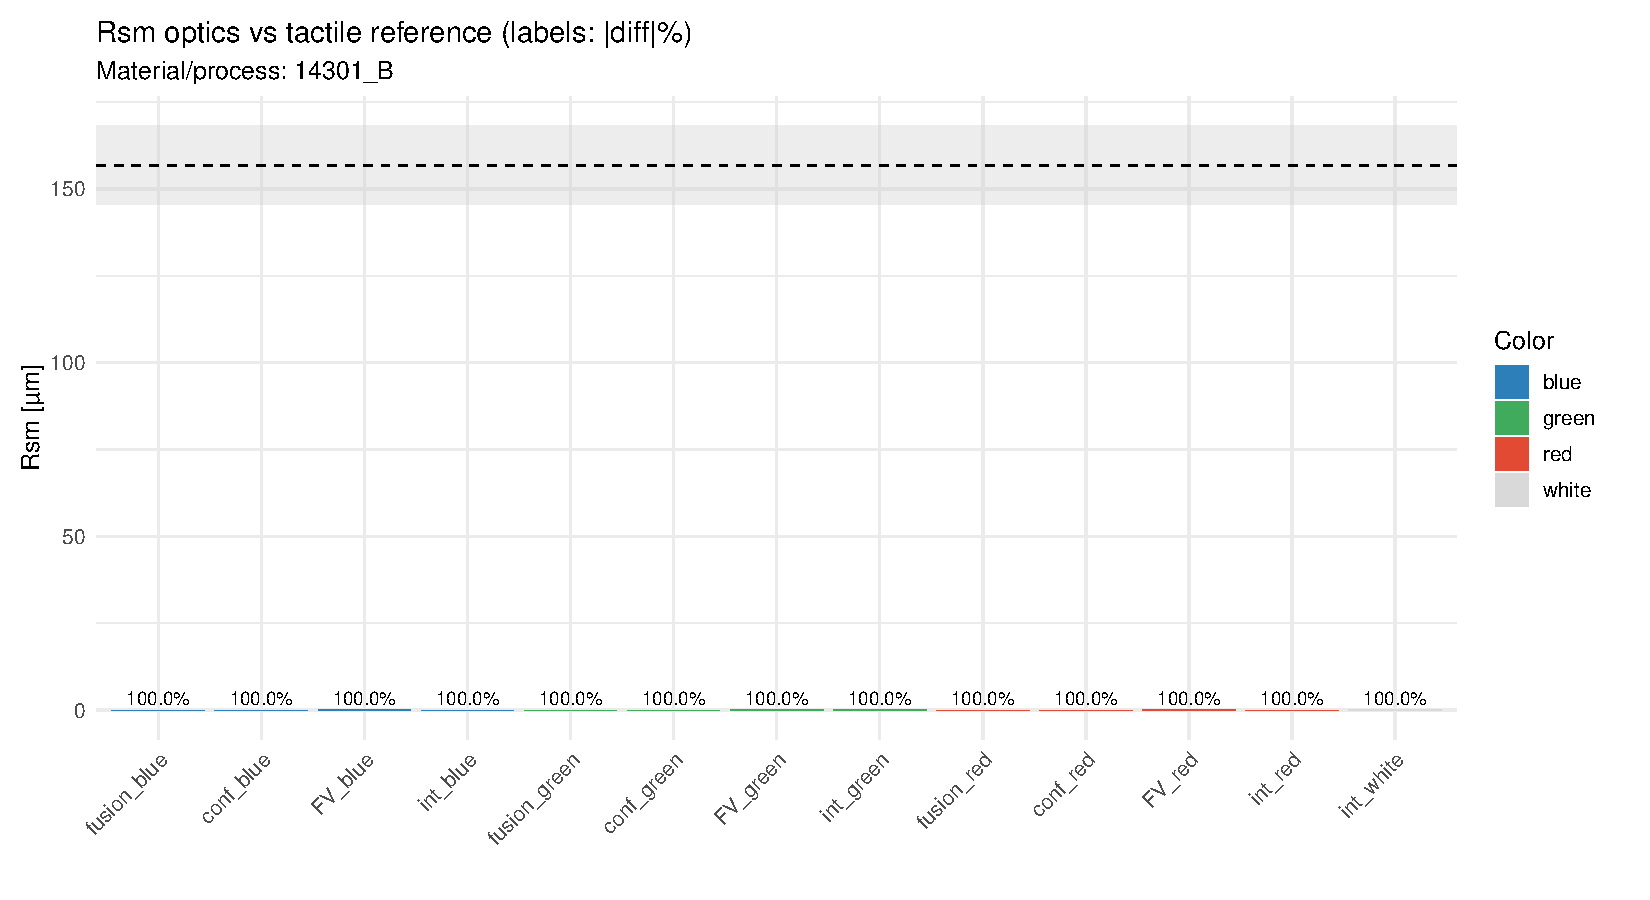
\includegraphics[width=\linewidth]{plots/rsm_abs_14301_b_optics_vs_tactile.pdf}
\end{minipage}
\begin{minipage}[t]{0.32\textwidth}\centering
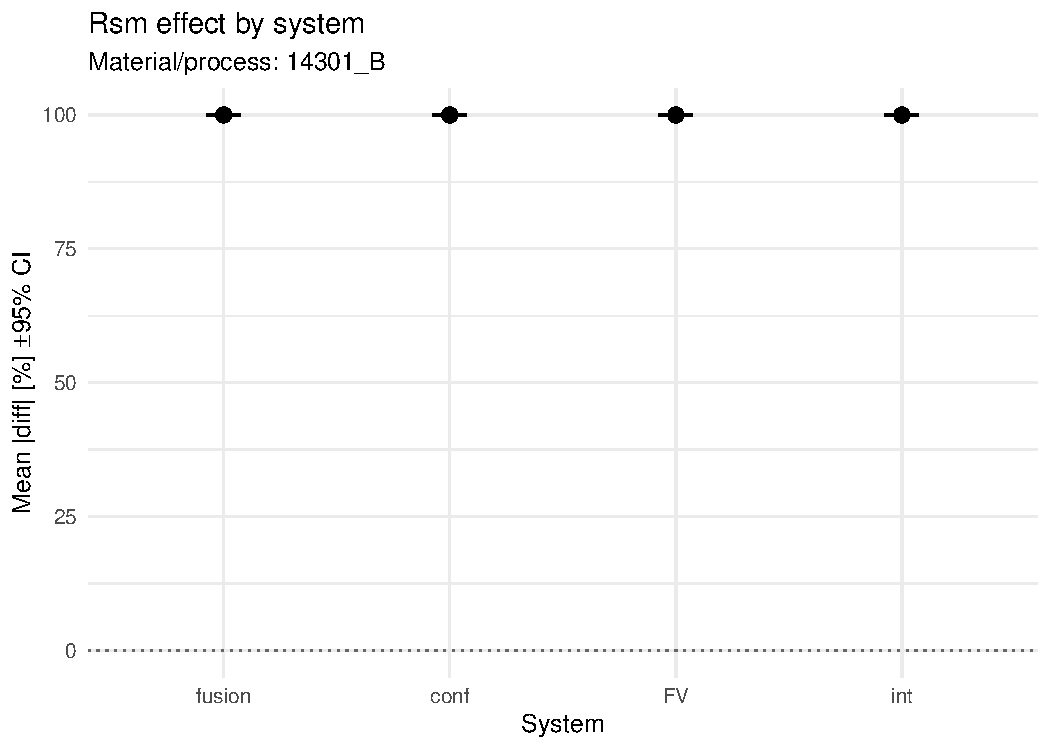
\includegraphics[width=\linewidth]{plots/rsm_abs_14301_b_effects_by_system.pdf}
\end{minipage}
\begin{minipage}[t]{0.32\textwidth}\centering
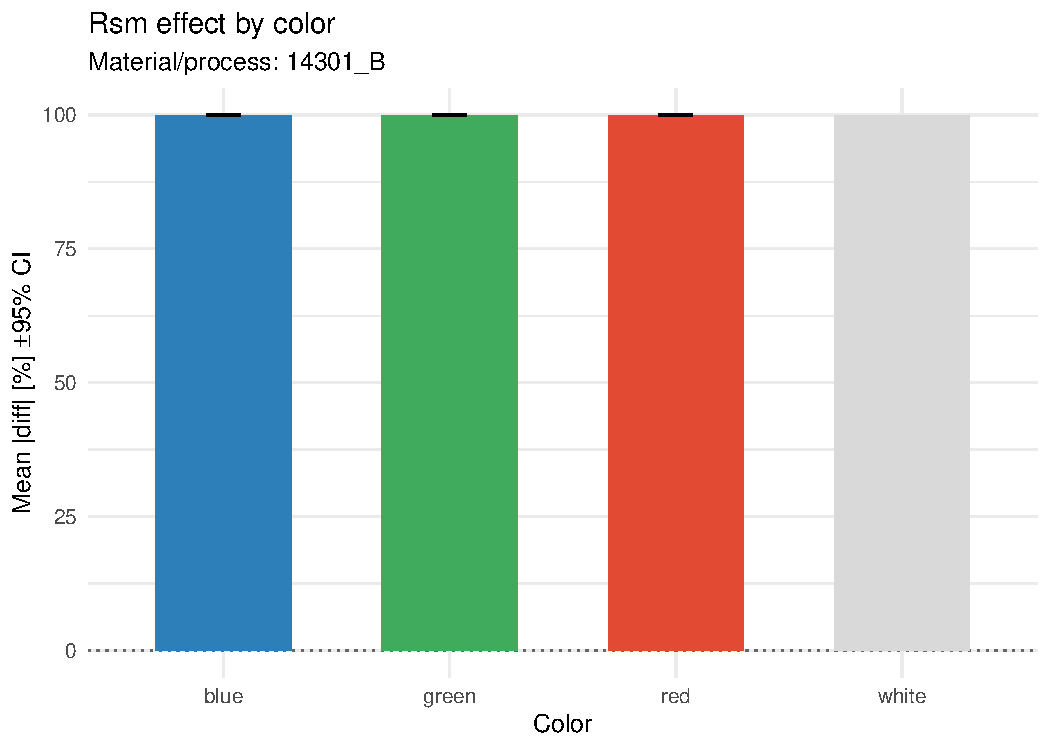
\includegraphics[width=\linewidth]{plots/rsm_abs_14301_b_effects_by_color.pdf}
\end{minipage}
\caption{RSM — 14301\_b — porównanie i efekty (|diff| \%)}
\end{figure}

\begin{figure}[H]\centering
\begin{minipage}[t]{0.32\textwidth}\centering
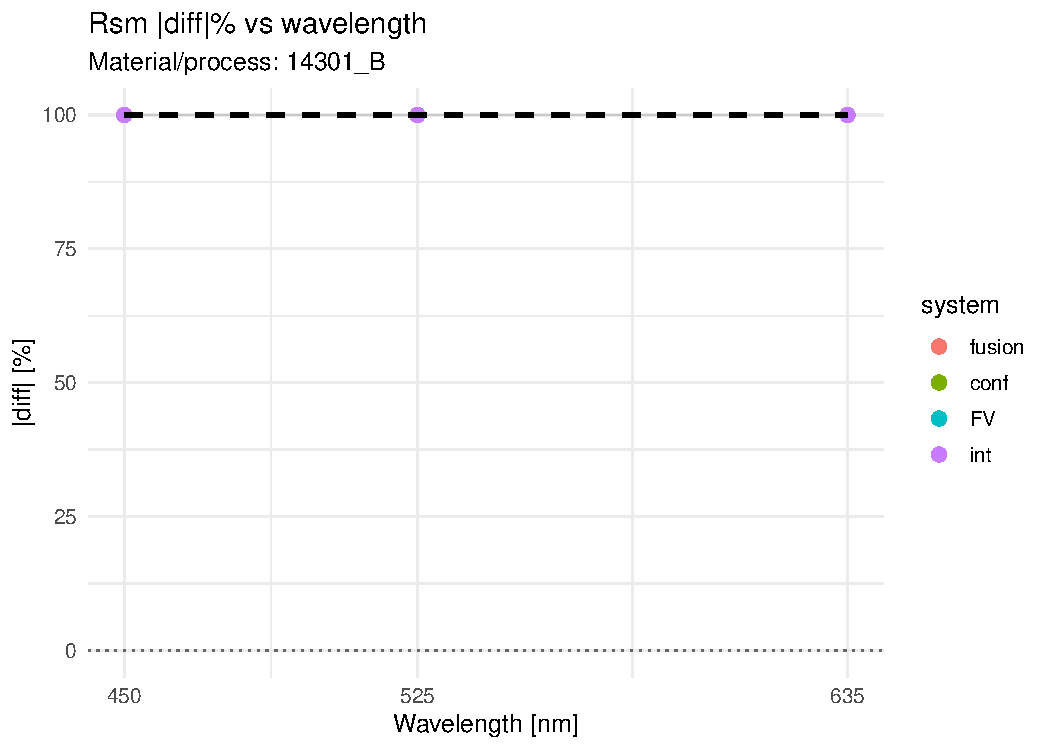
\includegraphics[width=\linewidth]{plots/rsm_abs_14301_b_diff_vs_wavelength.pdf}
\end{minipage}
\begin{minipage}[t]{0.32\textwidth}\centering
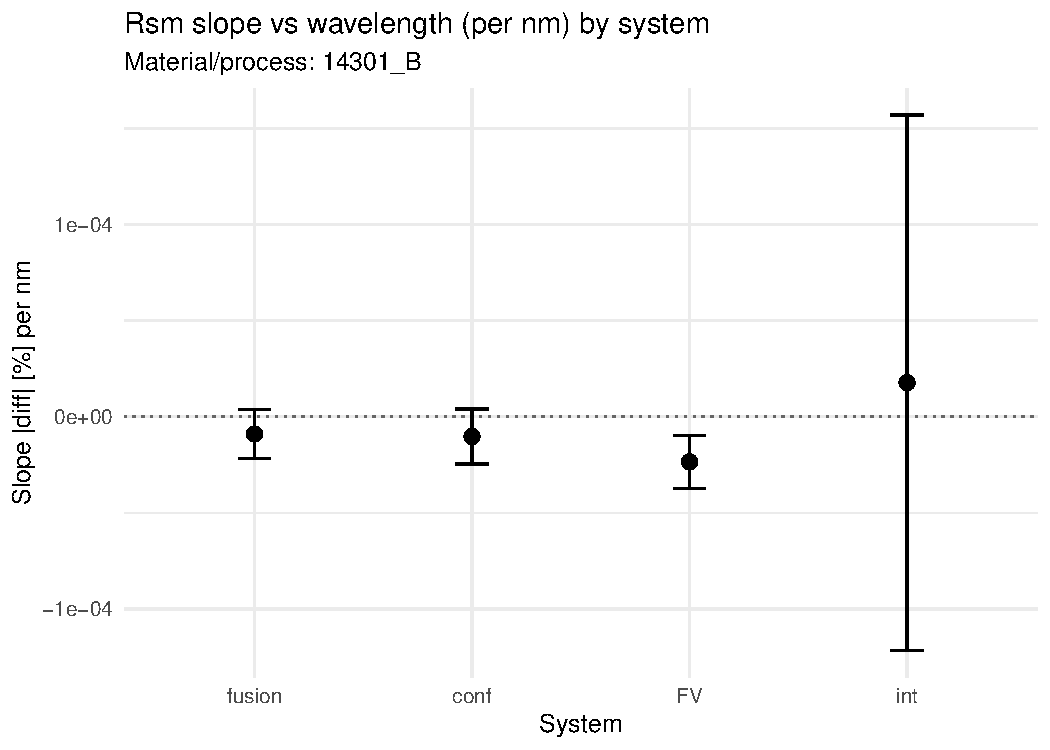
\includegraphics[width=\linewidth]{plots/rsm_abs_14301_b_slope_by_system_vs_nm.pdf}
\end{minipage}
\begin{minipage}[t]{0.32\textwidth}\centering
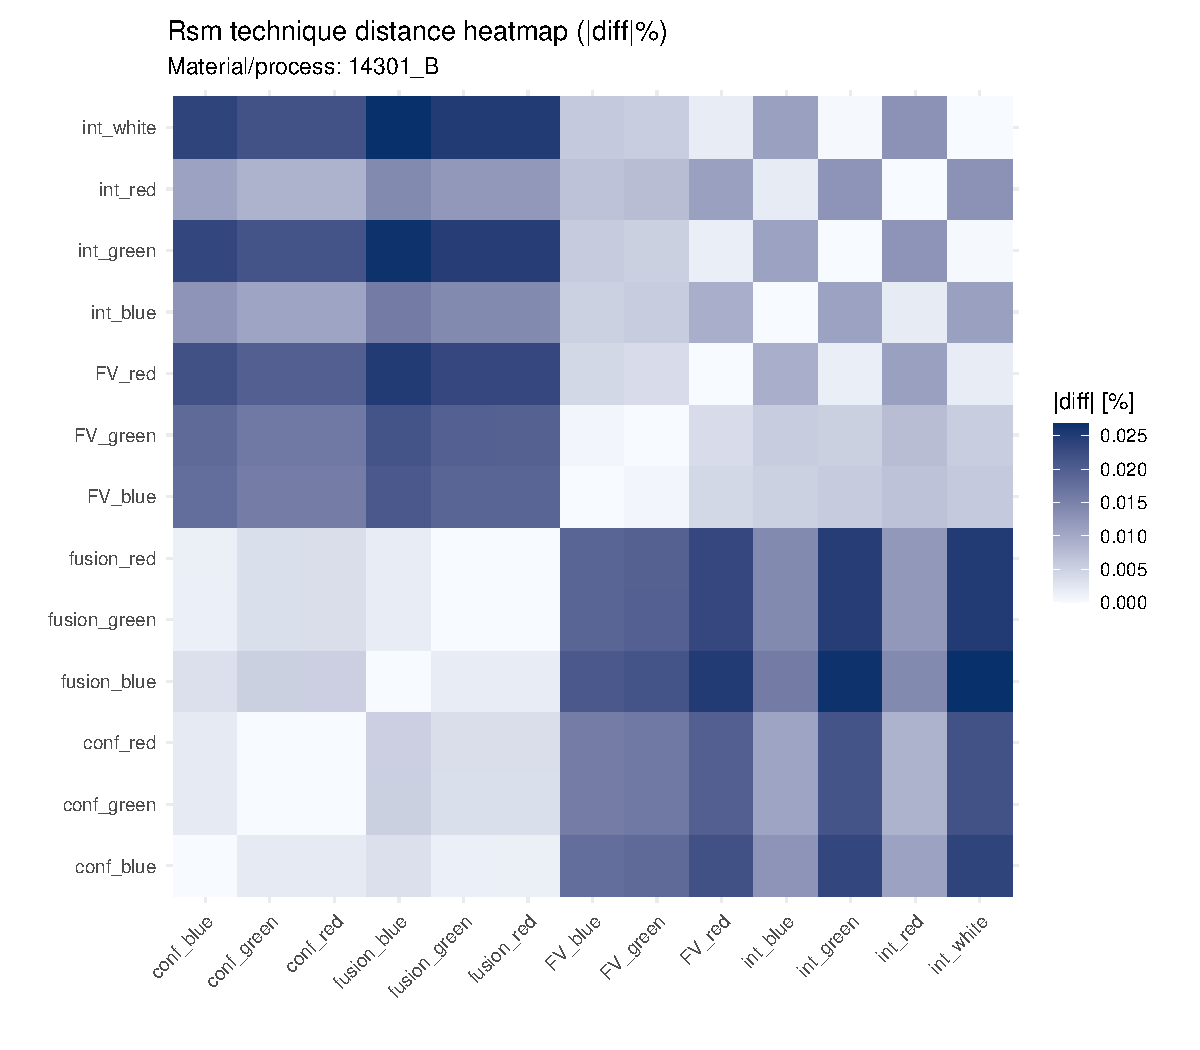
\includegraphics[width=\linewidth]{plots/rsm_abs_14301_b_tech_distance_heatmap.pdf}
\end{minipage}
\caption{RSM — 14301\_b — wavelength, nachylenia, odległości technik}
\end{figure}

\begin{figure}[H]\centering
\begin{minipage}[t]{0.32\textwidth}\centering
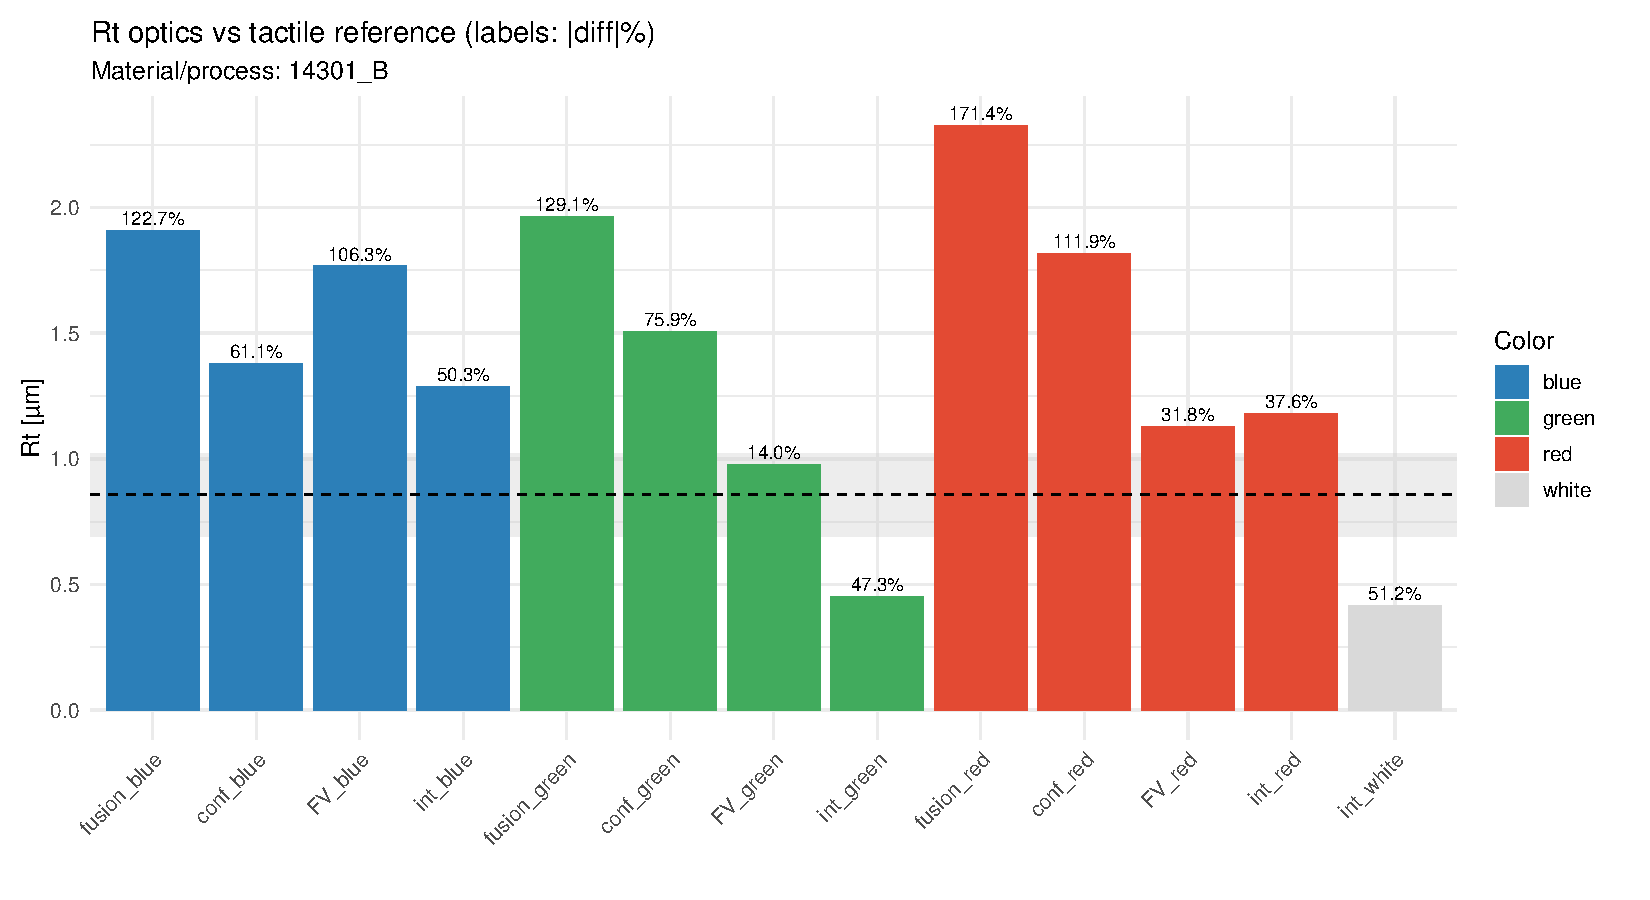
\includegraphics[width=\linewidth]{plots/rt_abs_14301_b_optics_vs_tactile.pdf}
\end{minipage}
\begin{minipage}[t]{0.32\textwidth}\centering
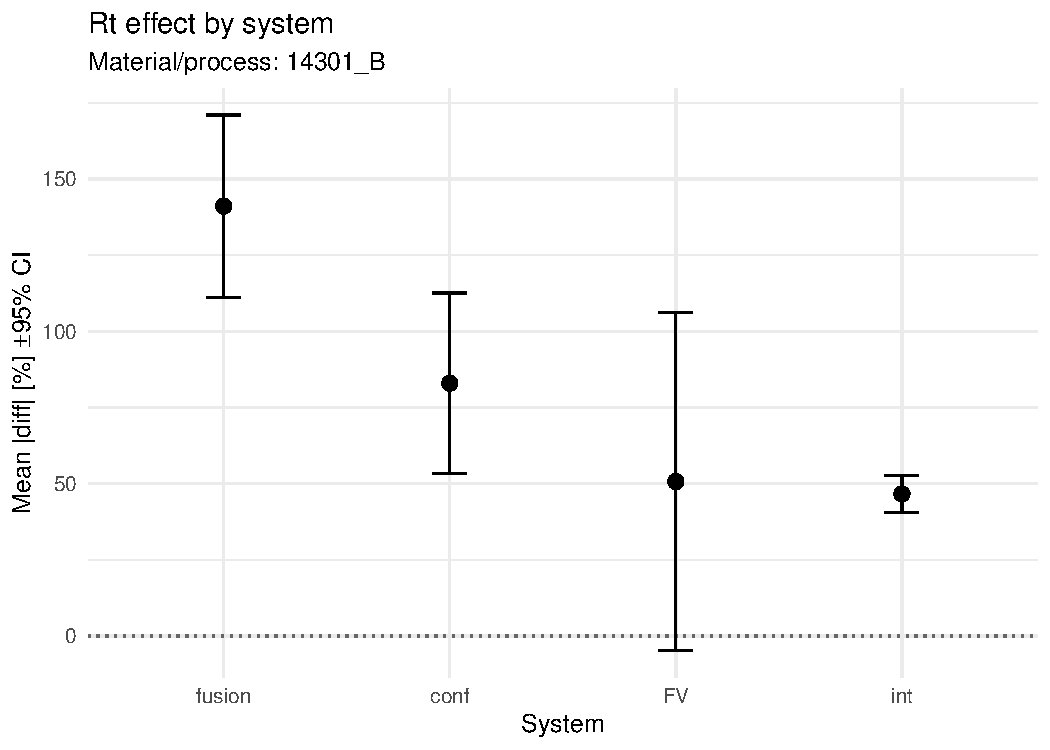
\includegraphics[width=\linewidth]{plots/rt_abs_14301_b_effects_by_system.pdf}
\end{minipage}
\begin{minipage}[t]{0.32\textwidth}\centering
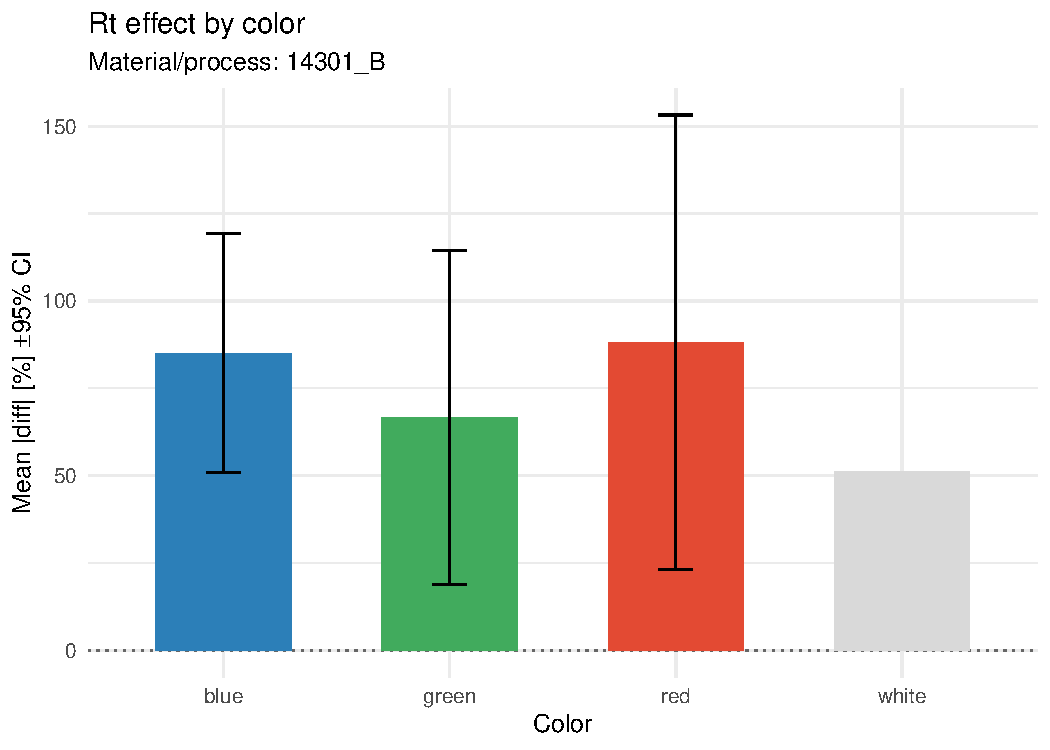
\includegraphics[width=\linewidth]{plots/rt_abs_14301_b_effects_by_color.pdf}
\end{minipage}
\caption{RT — 14301\_b — porównanie i efekty (|diff| \%)}
\end{figure}

\begin{figure}[H]\centering
\begin{minipage}[t]{0.32\textwidth}\centering
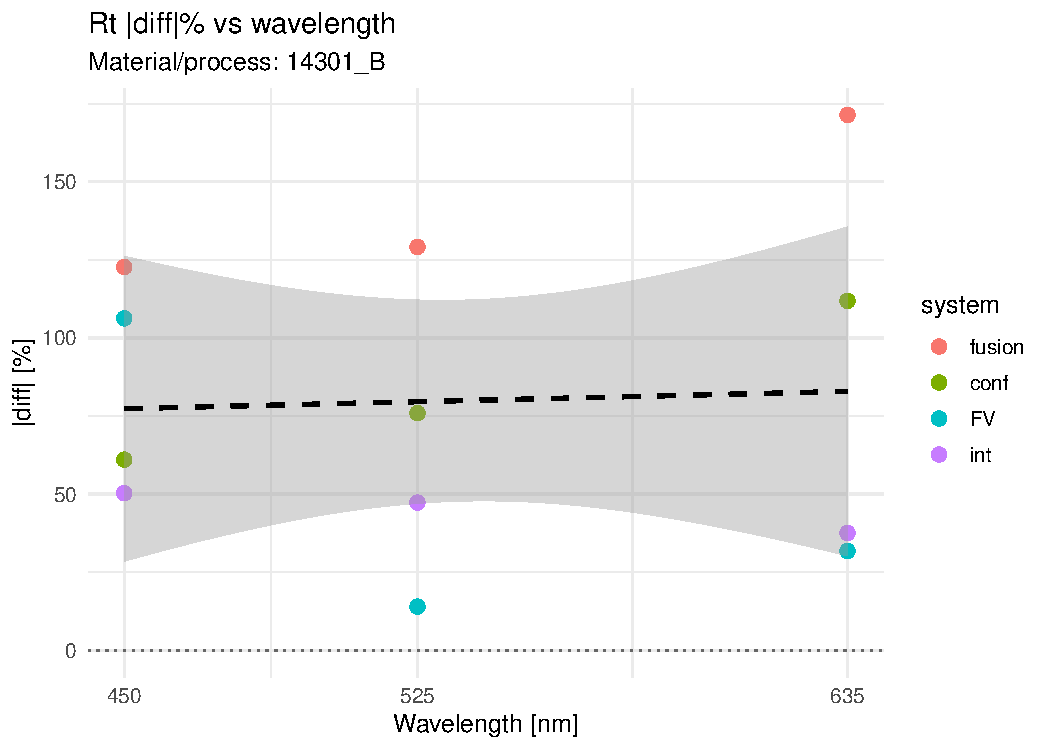
\includegraphics[width=\linewidth]{plots/rt_abs_14301_b_diff_vs_wavelength.pdf}
\end{minipage}
\begin{minipage}[t]{0.32\textwidth}\centering
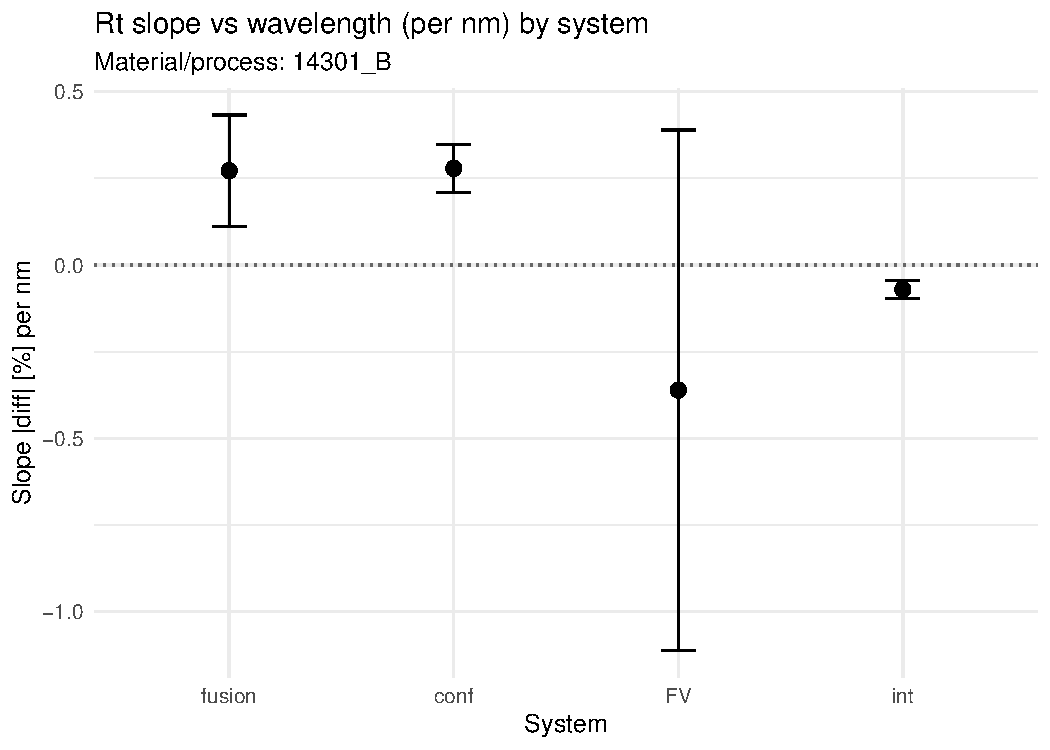
\includegraphics[width=\linewidth]{plots/rt_abs_14301_b_slope_by_system_vs_nm.pdf}
\end{minipage}
\begin{minipage}[t]{0.32\textwidth}\centering
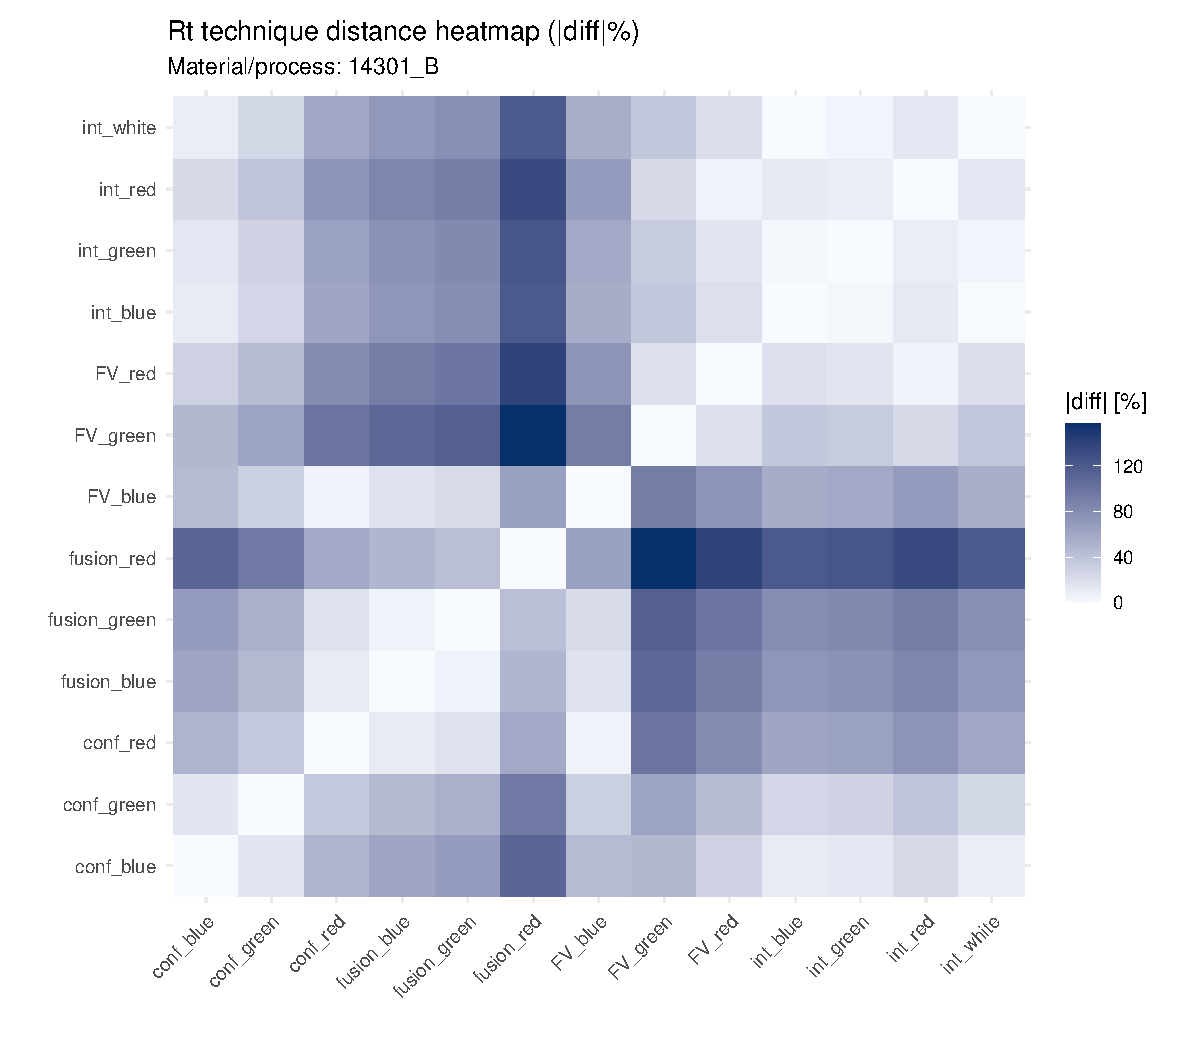
\includegraphics[width=\linewidth]{plots/rt_abs_14301_b_tech_distance_heatmap.pdf}
\end{minipage}
\caption{RT — 14301\_b — wavelength, nachylenia, odległości technik}
\end{figure}

\begin{figure}[H]\centering
\begin{minipage}[t]{0.32\textwidth}\centering
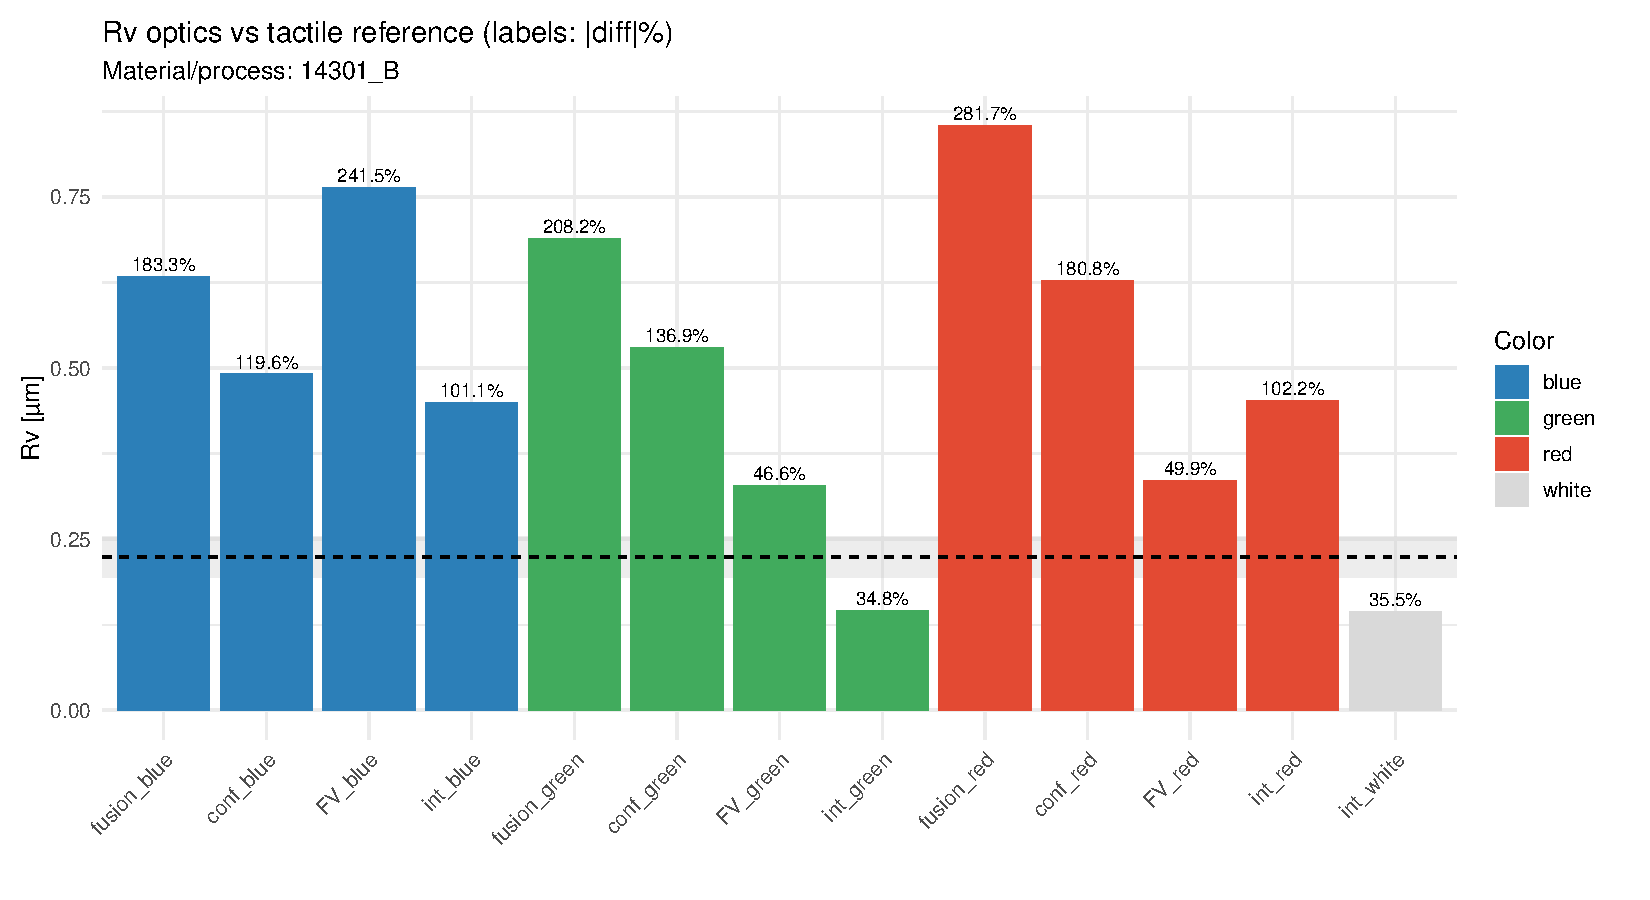
\includegraphics[width=\linewidth]{plots/rv_abs_14301_b_optics_vs_tactile.pdf}
\end{minipage}
\begin{minipage}[t]{0.32\textwidth}\centering
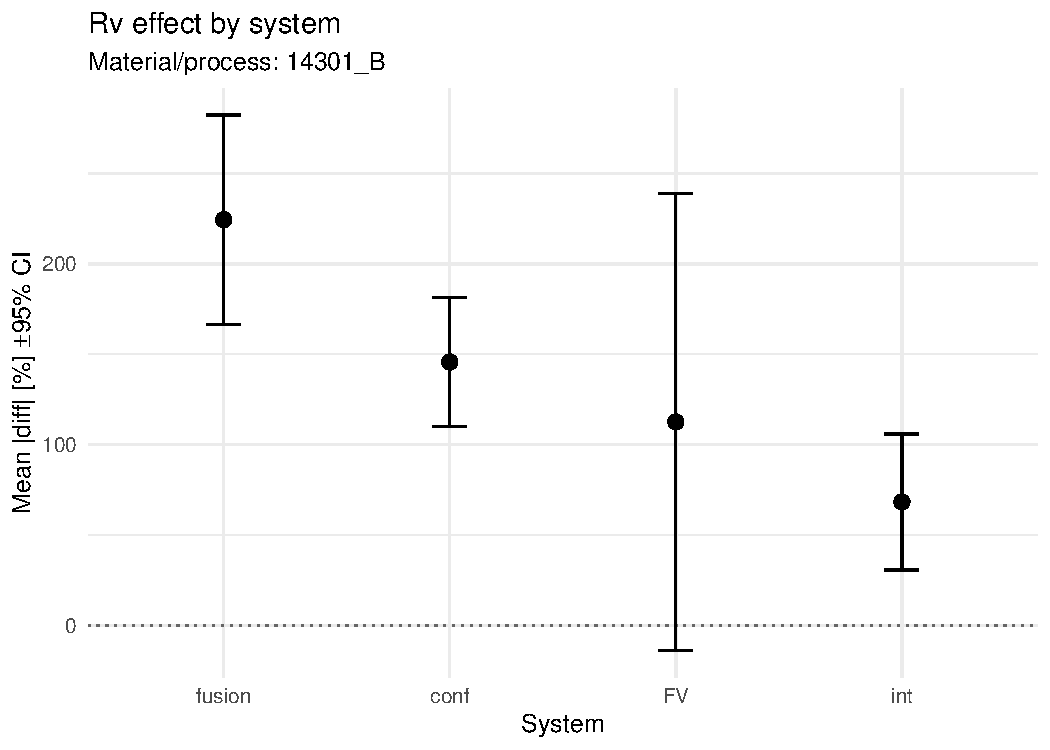
\includegraphics[width=\linewidth]{plots/rv_abs_14301_b_effects_by_system.pdf}
\end{minipage}
\begin{minipage}[t]{0.32\textwidth}\centering
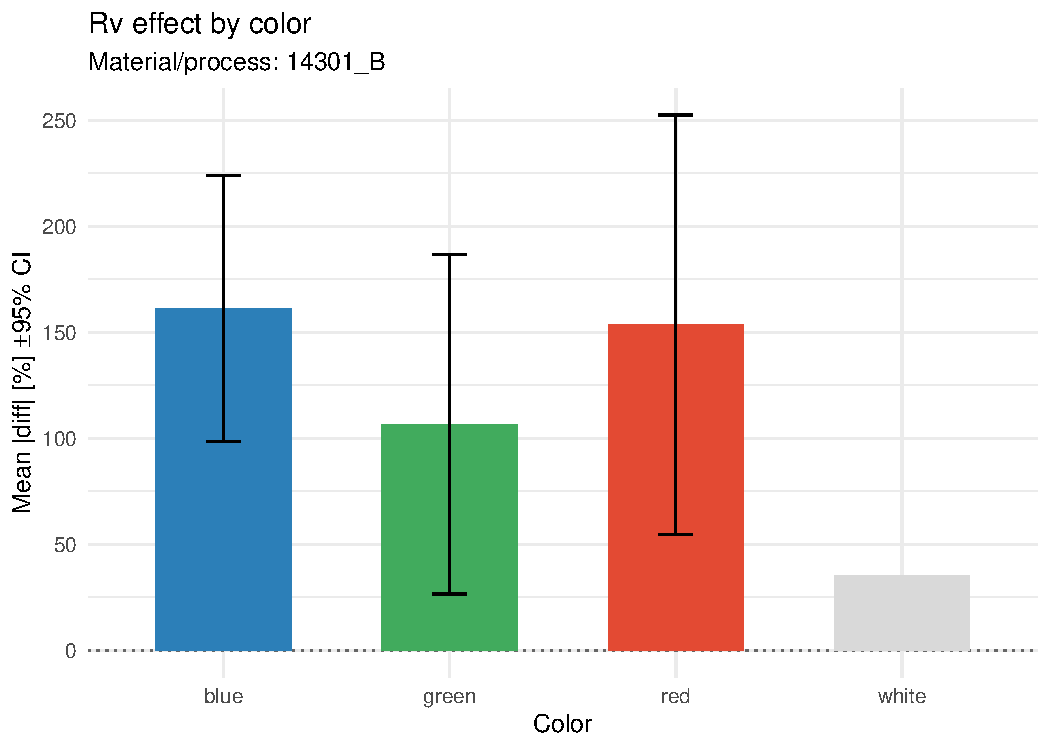
\includegraphics[width=\linewidth]{plots/rv_abs_14301_b_effects_by_color.pdf}
\end{minipage}
\caption{RV — 14301\_b — porównanie i efekty (|diff| \%)}
\end{figure}

\begin{figure}[H]\centering
\begin{minipage}[t]{0.32\textwidth}\centering
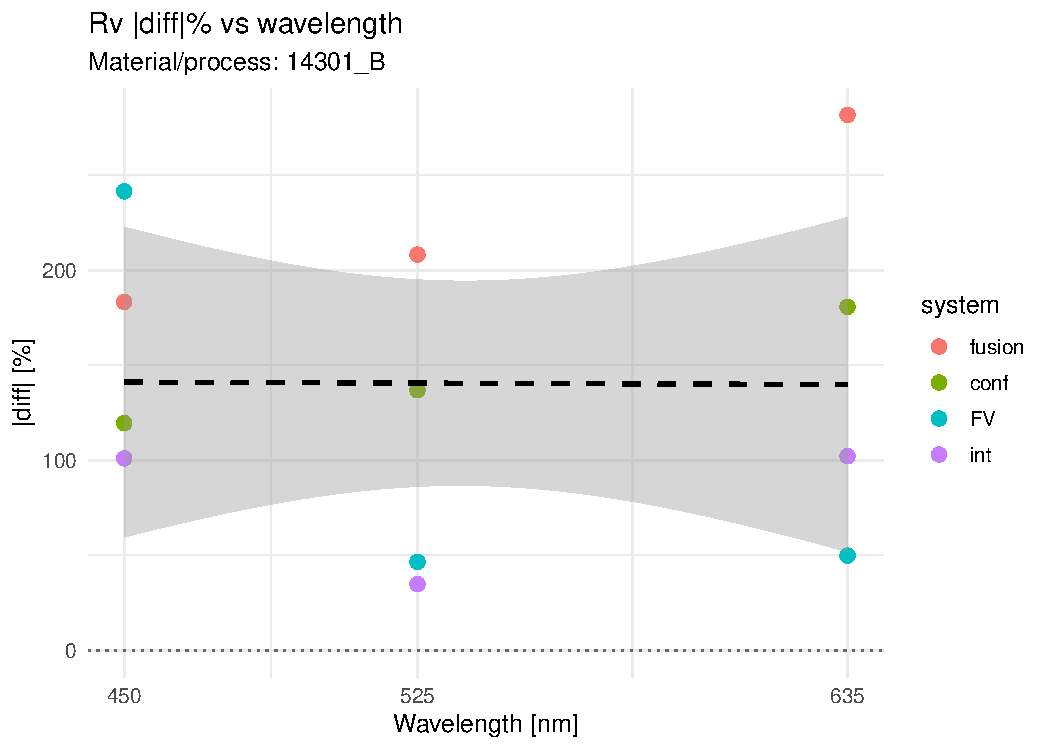
\includegraphics[width=\linewidth]{plots/rv_abs_14301_b_diff_vs_wavelength.pdf}
\end{minipage}
\begin{minipage}[t]{0.32\textwidth}\centering
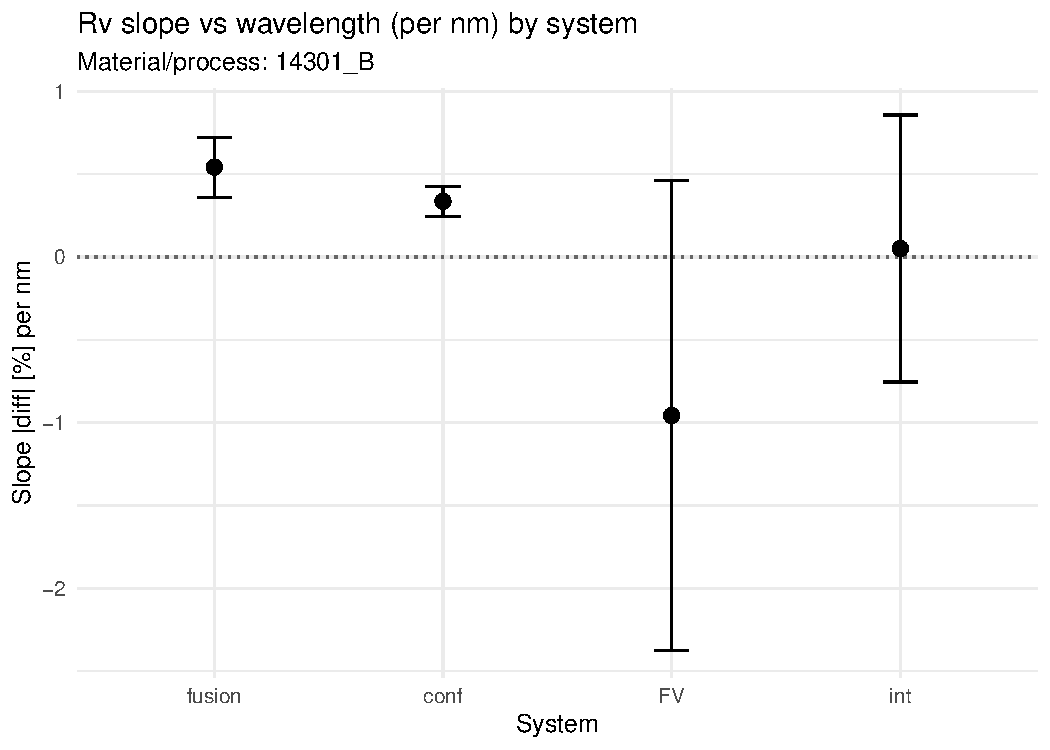
\includegraphics[width=\linewidth]{plots/rv_abs_14301_b_slope_by_system_vs_nm.pdf}
\end{minipage}
\begin{minipage}[t]{0.32\textwidth}\centering
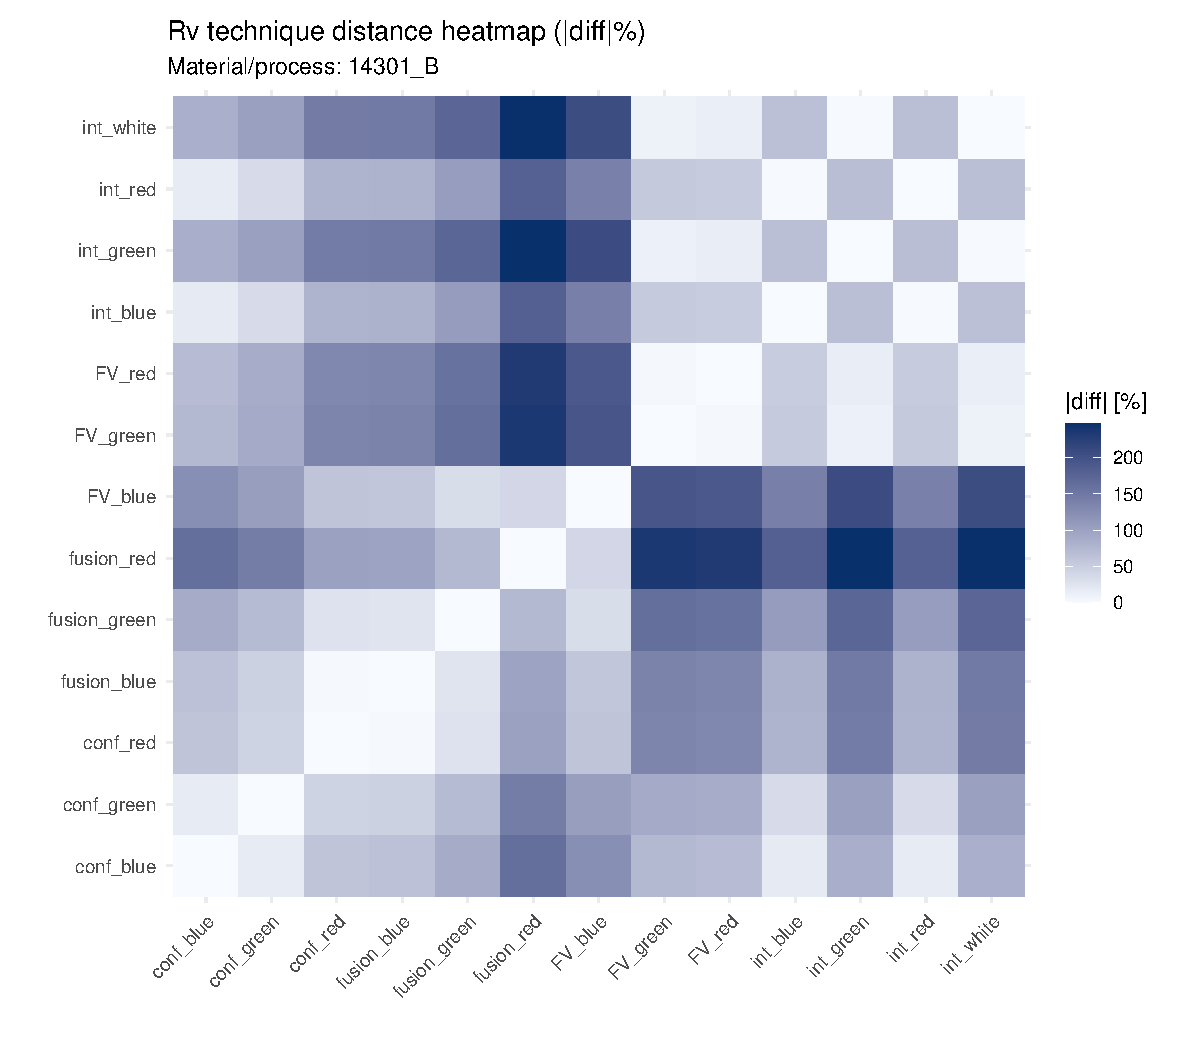
\includegraphics[width=\linewidth]{plots/rv_abs_14301_b_tech_distance_heatmap.pdf}
\end{minipage}
\caption{RV — 14301\_b — wavelength, nachylenia, odległości technik}
\end{figure}

\begin{figure}[H]\centering
\begin{minipage}[t]{0.32\textwidth}\centering
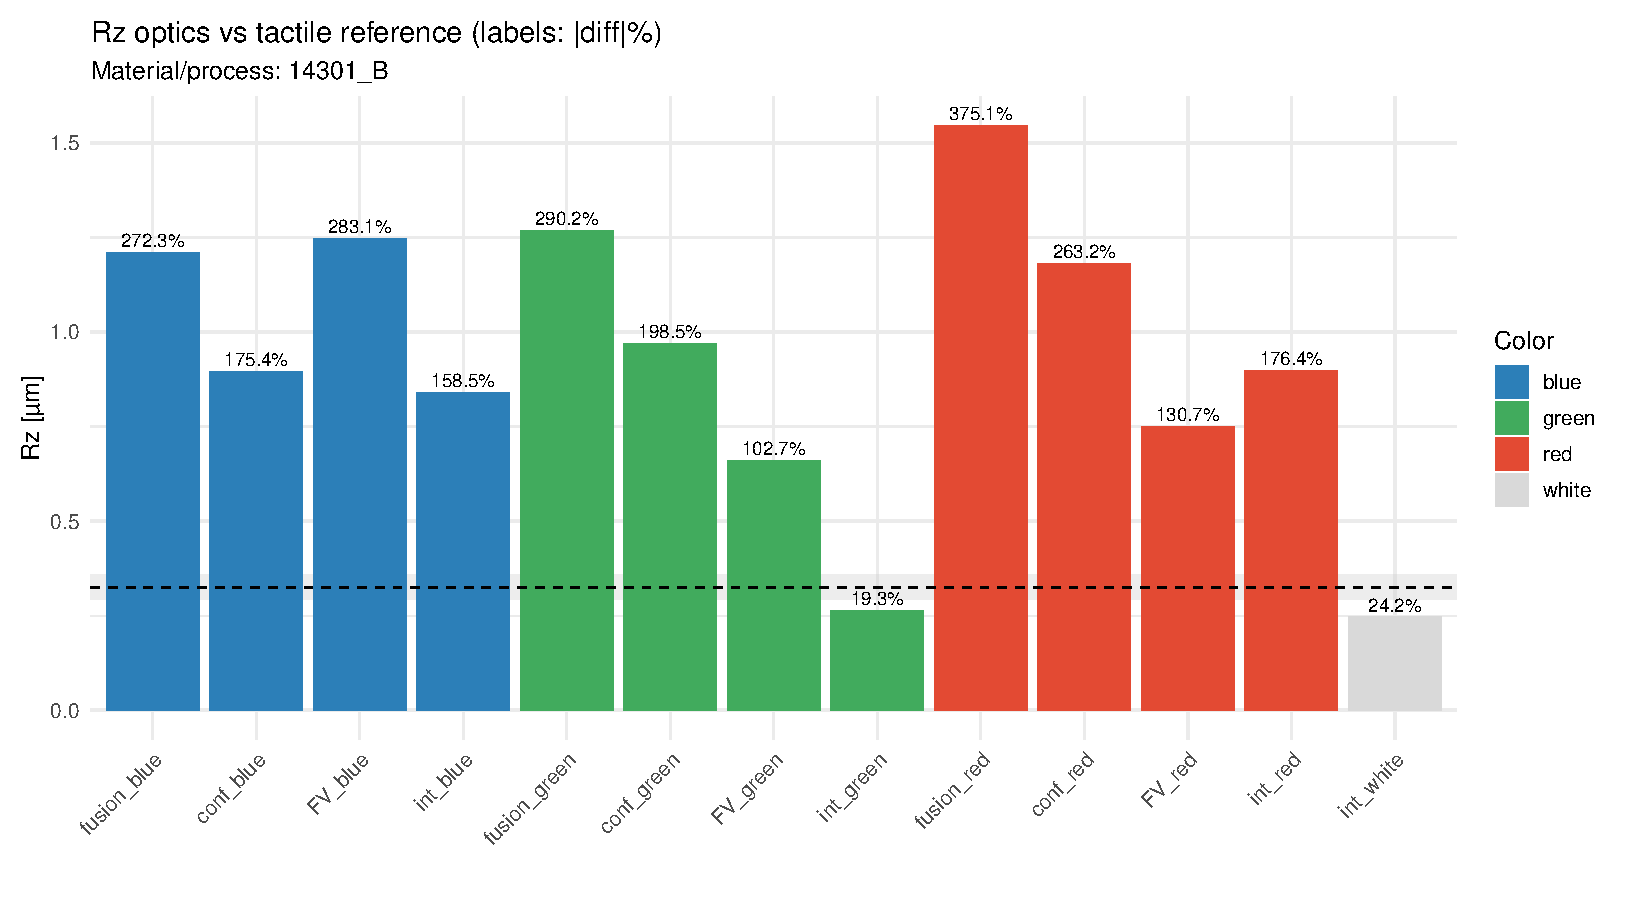
\includegraphics[width=\linewidth]{plots/rz_abs_14301_b_optics_vs_tactile.pdf}
\end{minipage}
\begin{minipage}[t]{0.32\textwidth}\centering
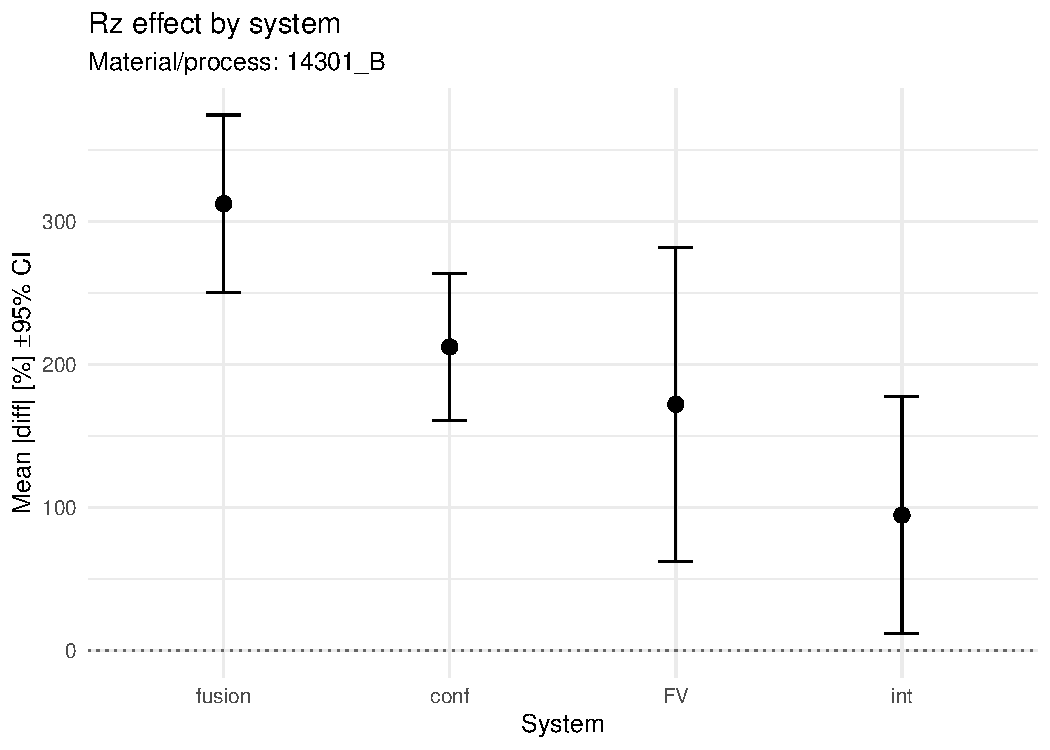
\includegraphics[width=\linewidth]{plots/rz_abs_14301_b_effects_by_system.pdf}
\end{minipage}
\begin{minipage}[t]{0.32\textwidth}\centering
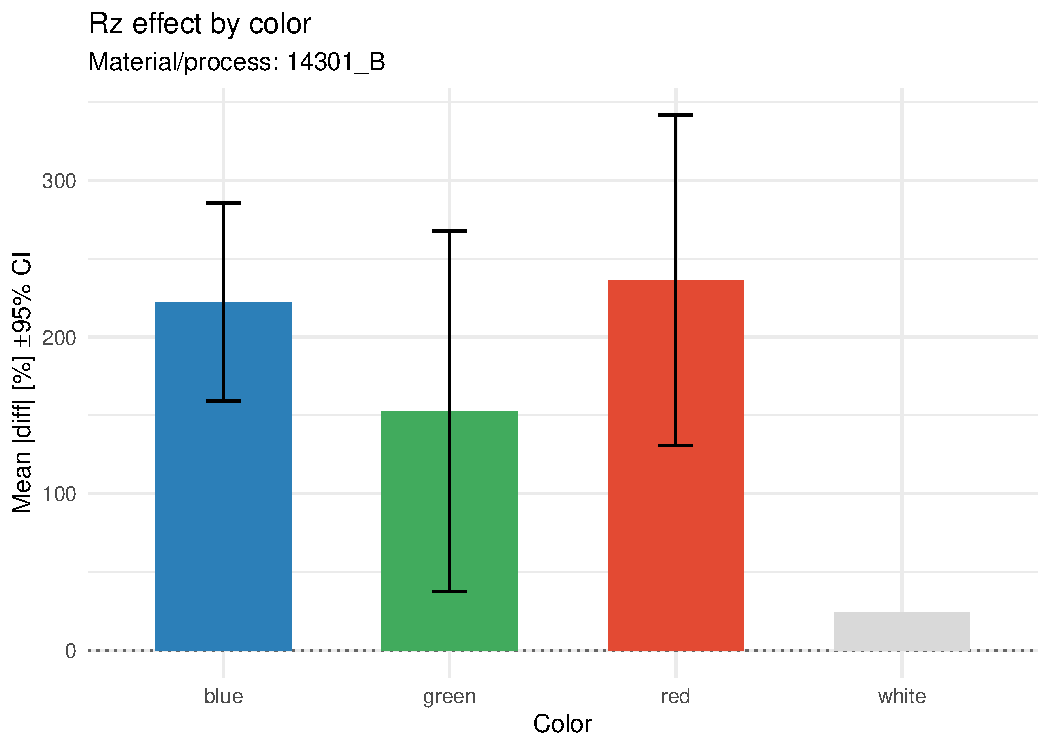
\includegraphics[width=\linewidth]{plots/rz_abs_14301_b_effects_by_color.pdf}
\end{minipage}
\caption{RZ — 14301\_b — porównanie i efekty (|diff| \%)}
\end{figure}

\begin{figure}[H]\centering
\begin{minipage}[t]{0.32\textwidth}\centering
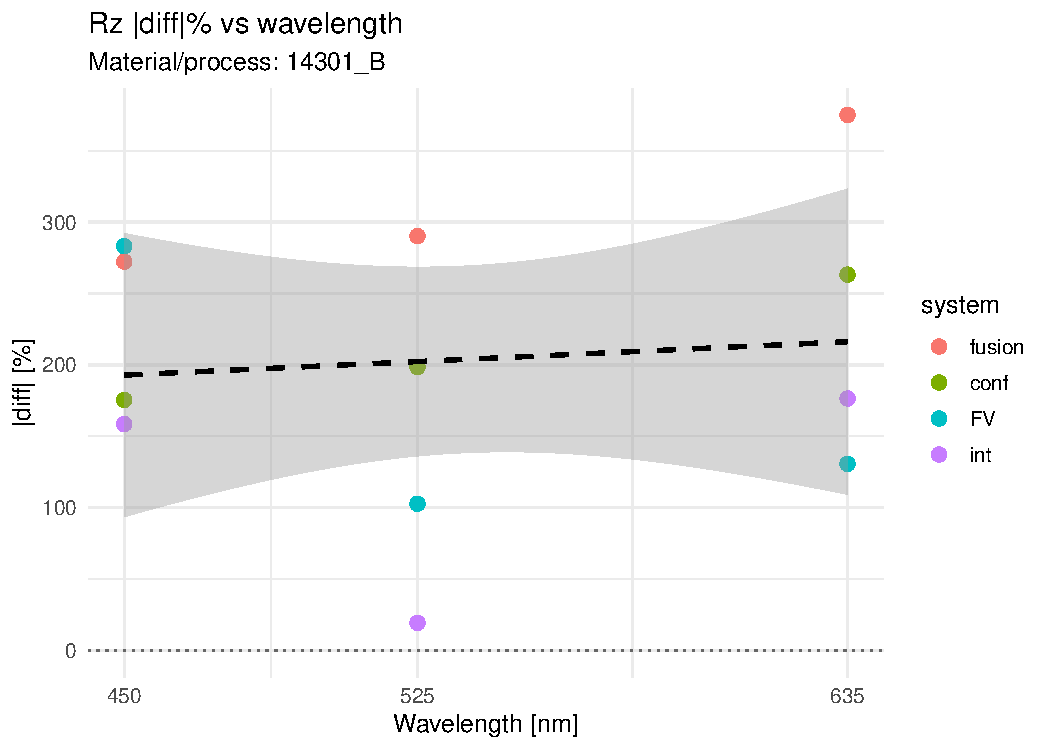
\includegraphics[width=\linewidth]{plots/rz_abs_14301_b_diff_vs_wavelength.pdf}
\end{minipage}
\begin{minipage}[t]{0.32\textwidth}\centering
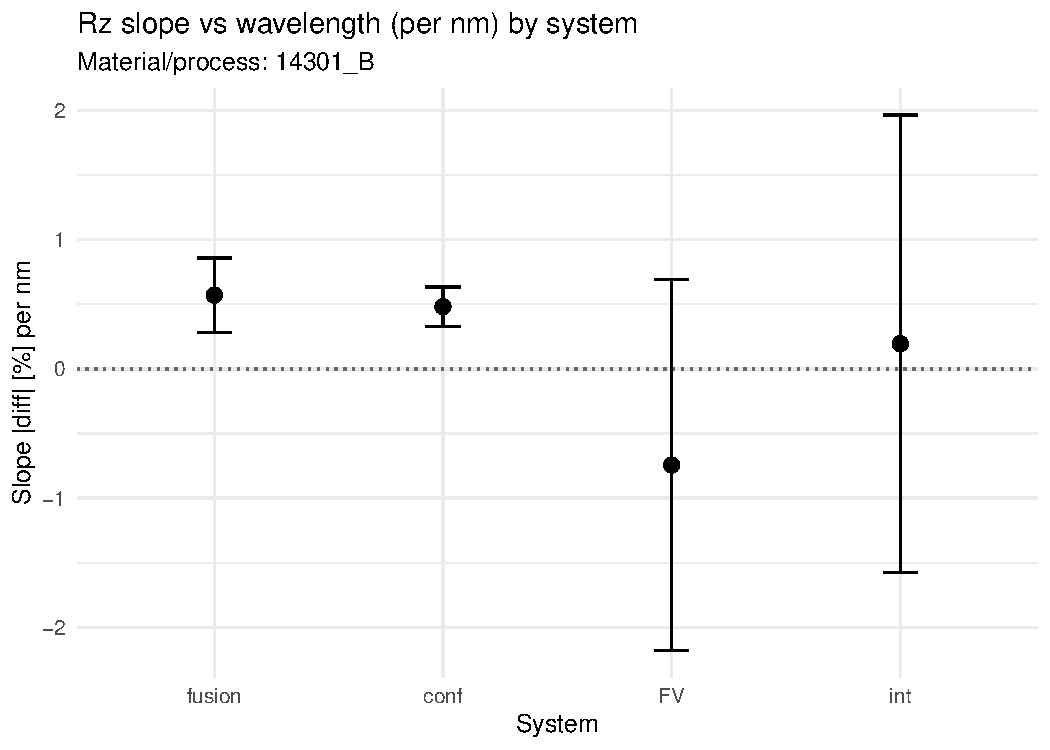
\includegraphics[width=\linewidth]{plots/rz_abs_14301_b_slope_by_system_vs_nm.pdf}
\end{minipage}
\begin{minipage}[t]{0.32\textwidth}\centering
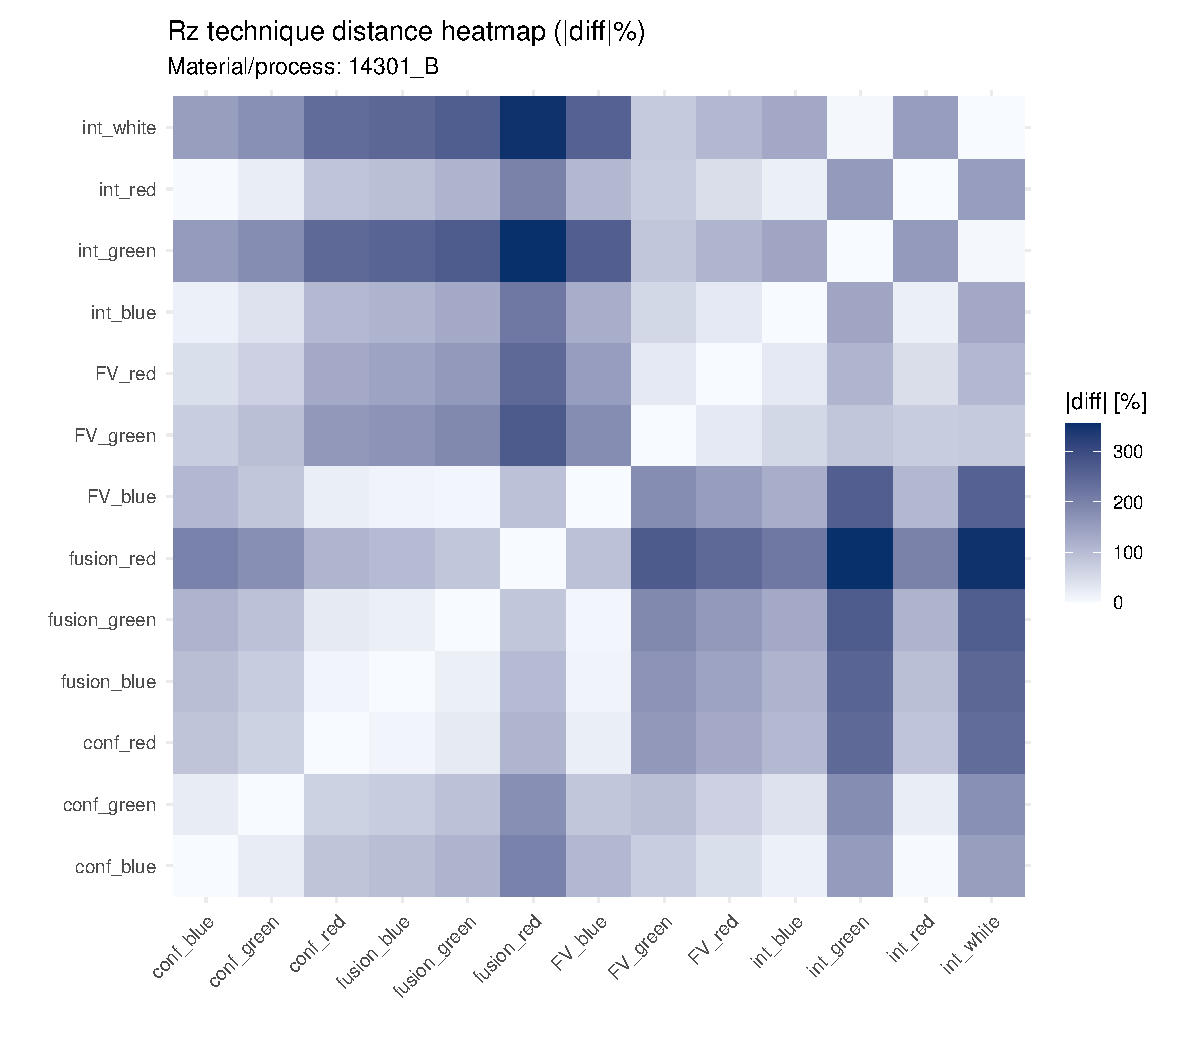
\includegraphics[width=\linewidth]{plots/rz_abs_14301_b_tech_distance_heatmap.pdf}
\end{minipage}
\caption{RZ — 14301\_b — wavelength, nachylenia, odległości technik}
\end{figure}

\begin{figure}[H]\centering
\begin{minipage}[t]{0.32\textwidth}\centering
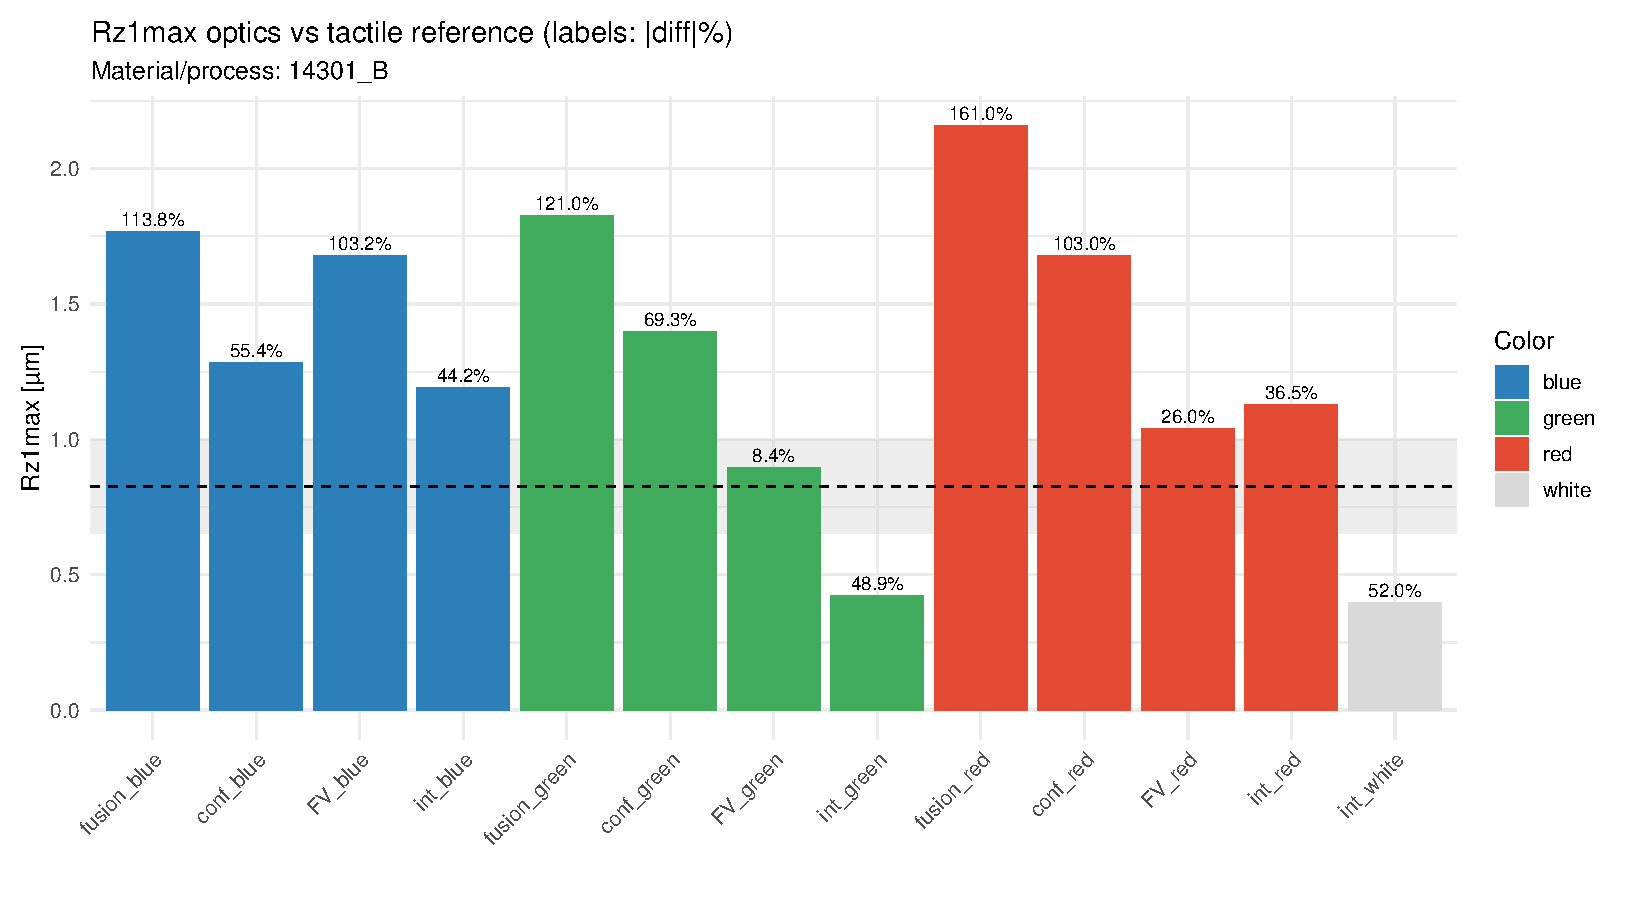
\includegraphics[width=\linewidth]{plots/rz1max_abs_14301_b_optics_vs_tactile.pdf}
\end{minipage}
\begin{minipage}[t]{0.32\textwidth}\centering
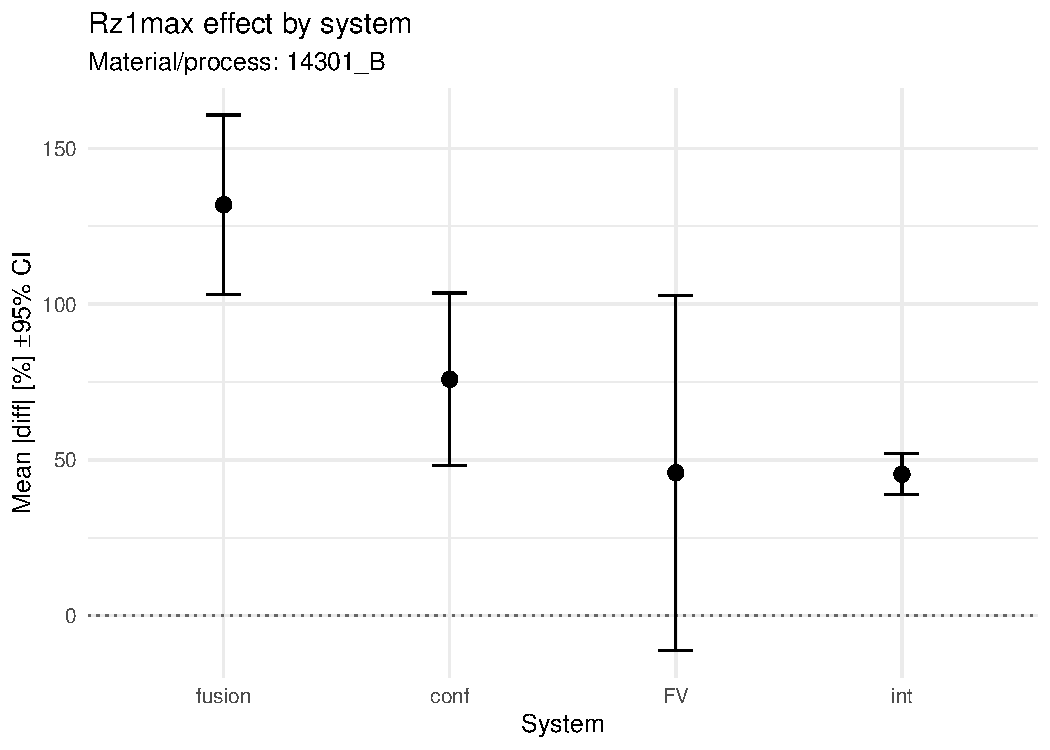
\includegraphics[width=\linewidth]{plots/rz1max_abs_14301_b_effects_by_system.pdf}
\end{minipage}
\begin{minipage}[t]{0.32\textwidth}\centering
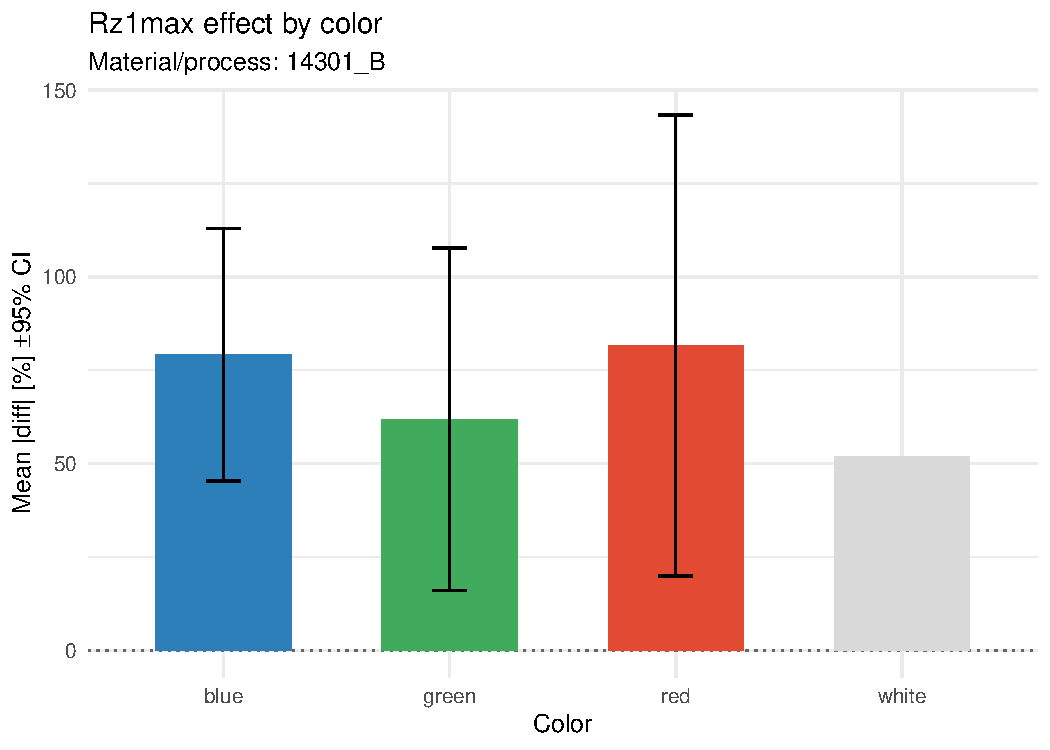
\includegraphics[width=\linewidth]{plots/rz1max_abs_14301_b_effects_by_color.pdf}
\end{minipage}
\caption{RZ1MAX — 14301\_b — porównanie i efekty (|diff| \%)}
\end{figure}

\begin{figure}[H]\centering
\begin{minipage}[t]{0.32\textwidth}\centering
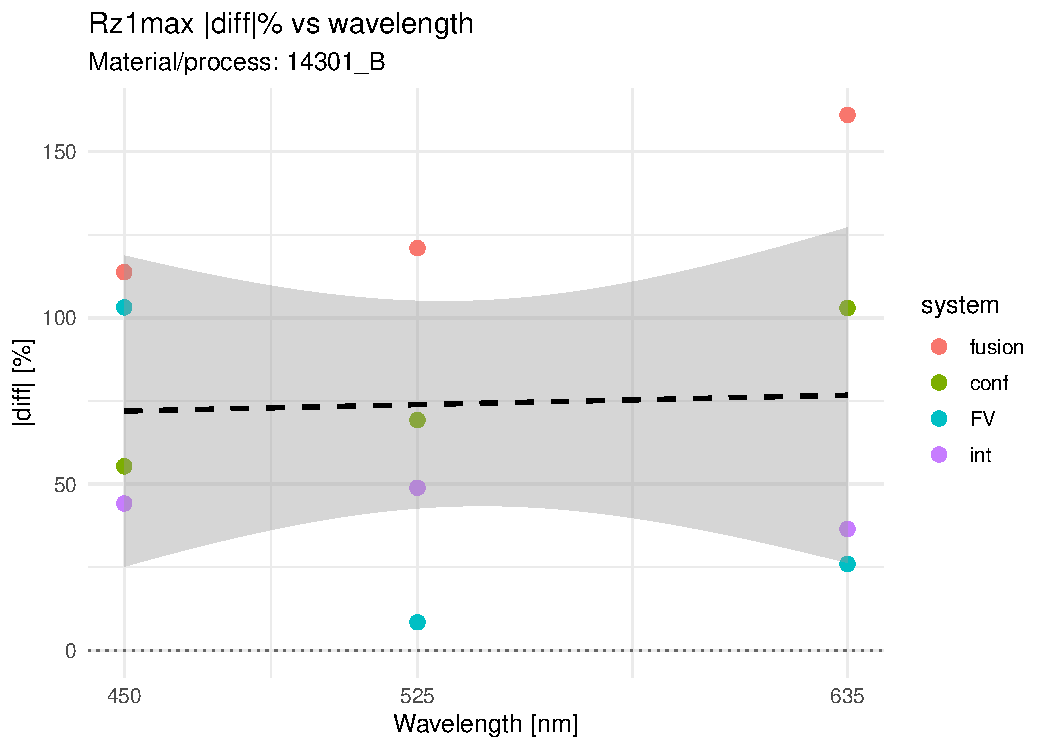
\includegraphics[width=\linewidth]{plots/rz1max_abs_14301_b_diff_vs_wavelength.pdf}
\end{minipage}
\begin{minipage}[t]{0.32\textwidth}\centering
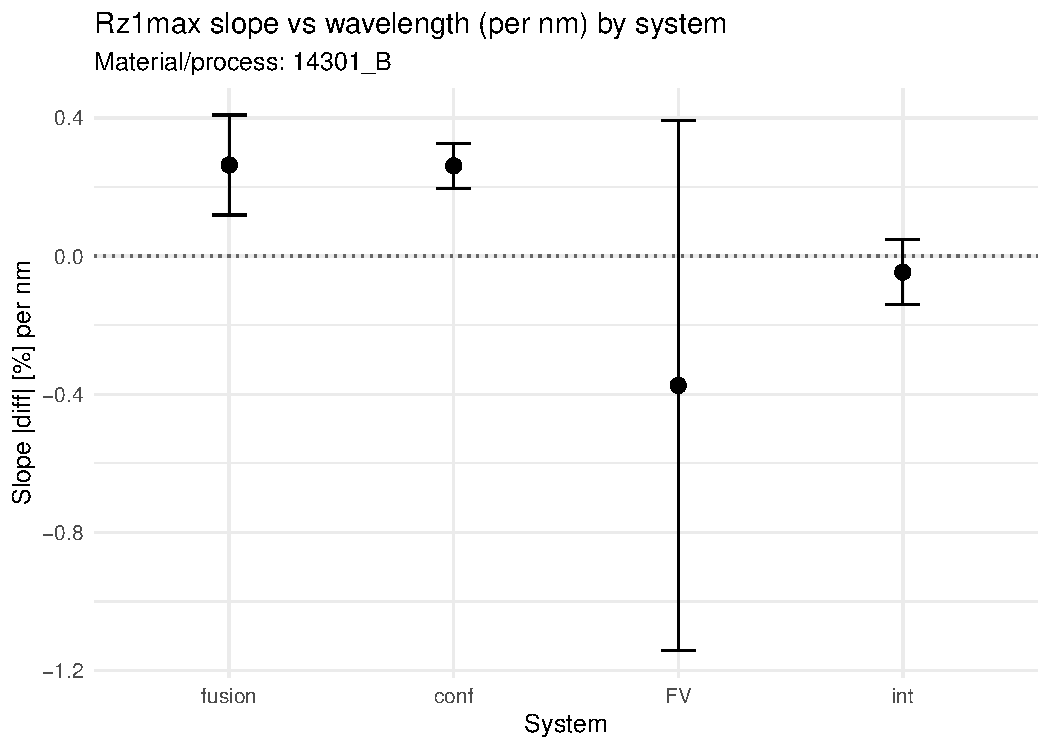
\includegraphics[width=\linewidth]{plots/rz1max_abs_14301_b_slope_by_system_vs_nm.pdf}
\end{minipage}
\begin{minipage}[t]{0.32\textwidth}\centering
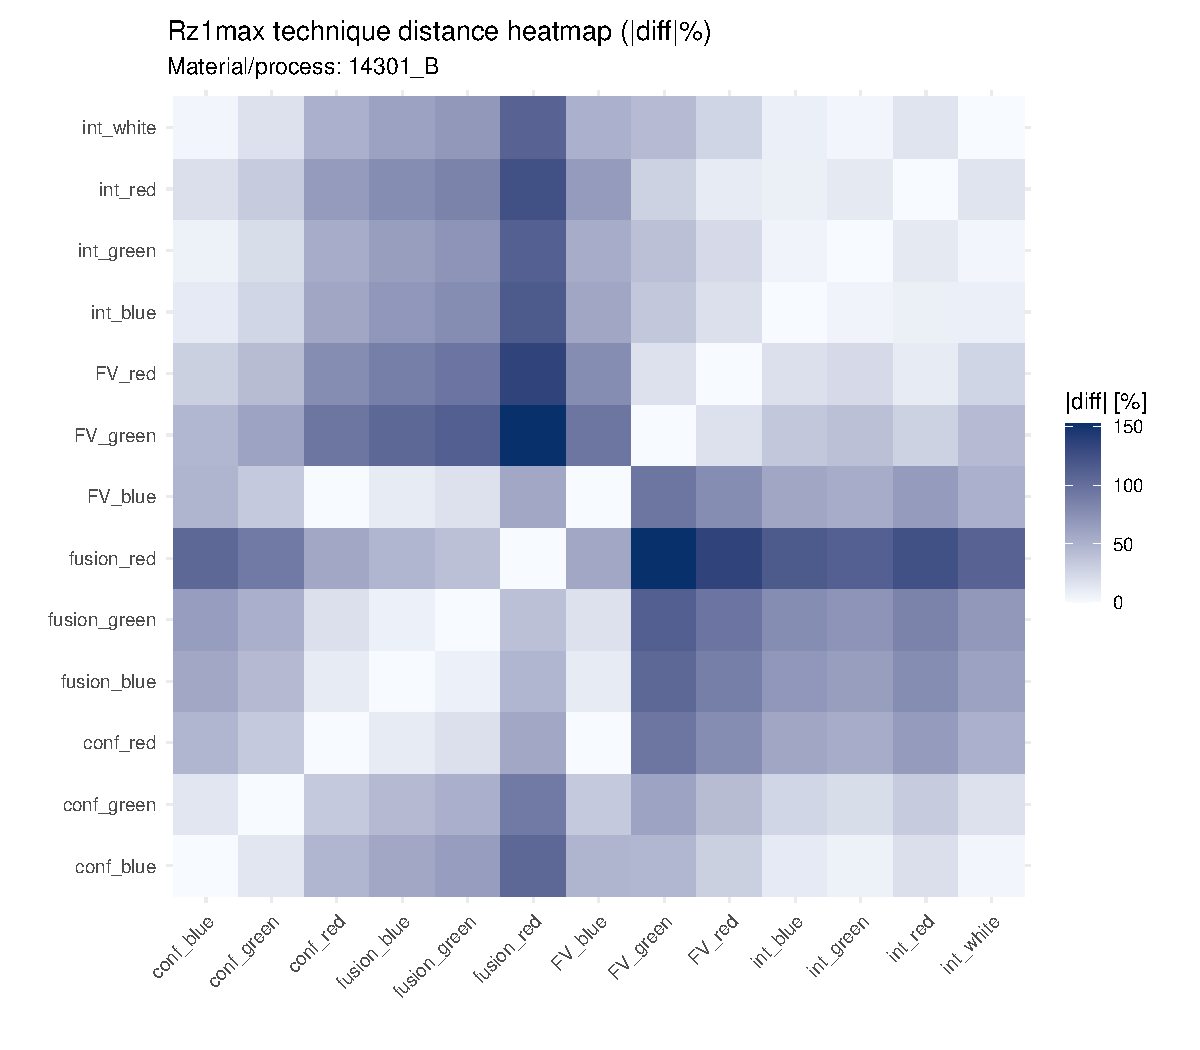
\includegraphics[width=\linewidth]{plots/rz1max_abs_14301_b_tech_distance_heatmap.pdf}
\end{minipage}
\caption{RZ1MAX — 14301\_b — wavelength, nachylenia, odległości technik}
\end{figure}

\subsection{Wyniki i wnioski dla materiał/proces: 14301\_b}

\textbf{RA}. r=0.100, rho=0.236; eta2: system=0.276, color=0.338.
Wniosek: NIE. \textbf{RKU}. r=0.009, rho=0.000; eta2: system=0.783,
color=0.022. Trendy (p\textless0.1): int(slope=0.036, p=0.075). Wniosek:
NIE. \textbf{RP}. r=0.229, rho=0.236; eta2: system=0.628, color=0.249.
Wniosek: NIE. \textbf{RQ}. r=0.111, rho=0.266; eta2: system=0.302,
color=0.301. Wniosek: NIE. \textbf{RSK}. r=0.591, rho=0.562; eta2:
system=0.121, color=0.392. Trendy (p\textless0.1): conf(slope=0.054,
p=0.051). Wniosek: NIE. \textbf{RSM}. r=-0.050, rho=-0.148; eta2:
system=0.879, color=0.060. Wniosek: NIE. \textbf{RT}. r=0.050,
rho=-0.089; eta2: system=0.703, color=0.043. Trendy (p\textless0.1):
conf(slope=0.279, p=0.081). Wniosek: NIE. \textbf{RV}. r=-0.007,
rho=-0.059; eta2: system=0.543, color=0.106. Trendy (p\textless0.1):
conf(slope=0.336, p=0.087). Wniosek: NIE. \textbf{RZ}. r=0.103,
rho=0.030; eta2: system=0.624, color=0.169. Wniosek: NIE.
\textbf{RZ1MAX}. r=0.045, rho=-0.118; eta2: system=0.671, color=0.042.
Trendy (p\textless0.1): conf(slope=0.261, p=0.081). Wniosek: NIE.

\paragraph{Podsumowanie (opisowe) dla tego materiału/procesu}
\begin{itemize}
\item W ujęciu ANOVA: częściej dominuje system (eta²).
\item Najczęściej preferowany system (min średni |diff|): int.
\item Najczęściej preferowana barwa (min średni |diff|): white.
\item Brak istotnych zależności od wavelength (p<0.05); trendy (p<0.1) dla parametrów: RKU, RSK, RT, RV, RZ1MAX; dotyczy systemów: int, conf.
\end{itemize}
\paragraph{Rekomendacje dla tego materiału}
\begin{itemize}
\item RA: preferowany system (min średni |diff|): int; preferowana barwa (min średni |diff|): white; dominuje barwa (color); zależność od wavelength: NIE (brak wykrytego trendu per system).
\item RKU: preferowany system (min średni |diff|): fusion; preferowana barwa (min średni |diff|): green; dominuje system; zależność od wavelength: trend (p<0.1) — int: rośnie.
\item RP: preferowany system (min średni |diff|): int; preferowana barwa (min średni |diff|): white; dominuje system; zależność od wavelength: NIE (brak wykrytego trendu per system).
\item RQ: preferowany system (min średni |diff|): int; preferowana barwa (min średni |diff|): white; system i barwa (color) mają podobny wpływ; zależność od wavelength: NIE (brak wykrytego trendu per system).
\item RSK: preferowany system (min średni |diff|): fusion; preferowana barwa (min średni |diff|): blue; dominuje barwa (color); zależność od wavelength: trend (p<0.1) — conf: rośnie.
\item RSM: preferowany system (min średni |diff|): FV; preferowana barwa (min średni |diff|): white; dominuje system; zależność od wavelength: NIE (brak wykrytego trendu per system).
\item RT: preferowany system (min średni |diff|): int; preferowana barwa (min średni |diff|): white; dominuje system; zależność od wavelength: trend (p<0.1) — conf: rośnie.
\item RV: preferowany system (min średni |diff|): int; preferowana barwa (min średni |diff|): white; dominuje system; zależność od wavelength: trend (p<0.1) — conf: rośnie.
\item RZ: preferowany system (min średni |diff|): int; preferowana barwa (min średni |diff|): white; dominuje system; zależność od wavelength: NIE (brak wykrytego trendu per system).
\item RZ1MAX: preferowany system (min średni |diff|): int; preferowana barwa (min średni |diff|): white; dominuje system; zależność od wavelength: trend (p<0.1) — conf: rośnie.
\end{itemize}
\subsubsection{Materiał/proces: 14301\_gla}
\begin{figure}[H]\centering
\begin{minipage}[t]{0.32\textwidth}\centering
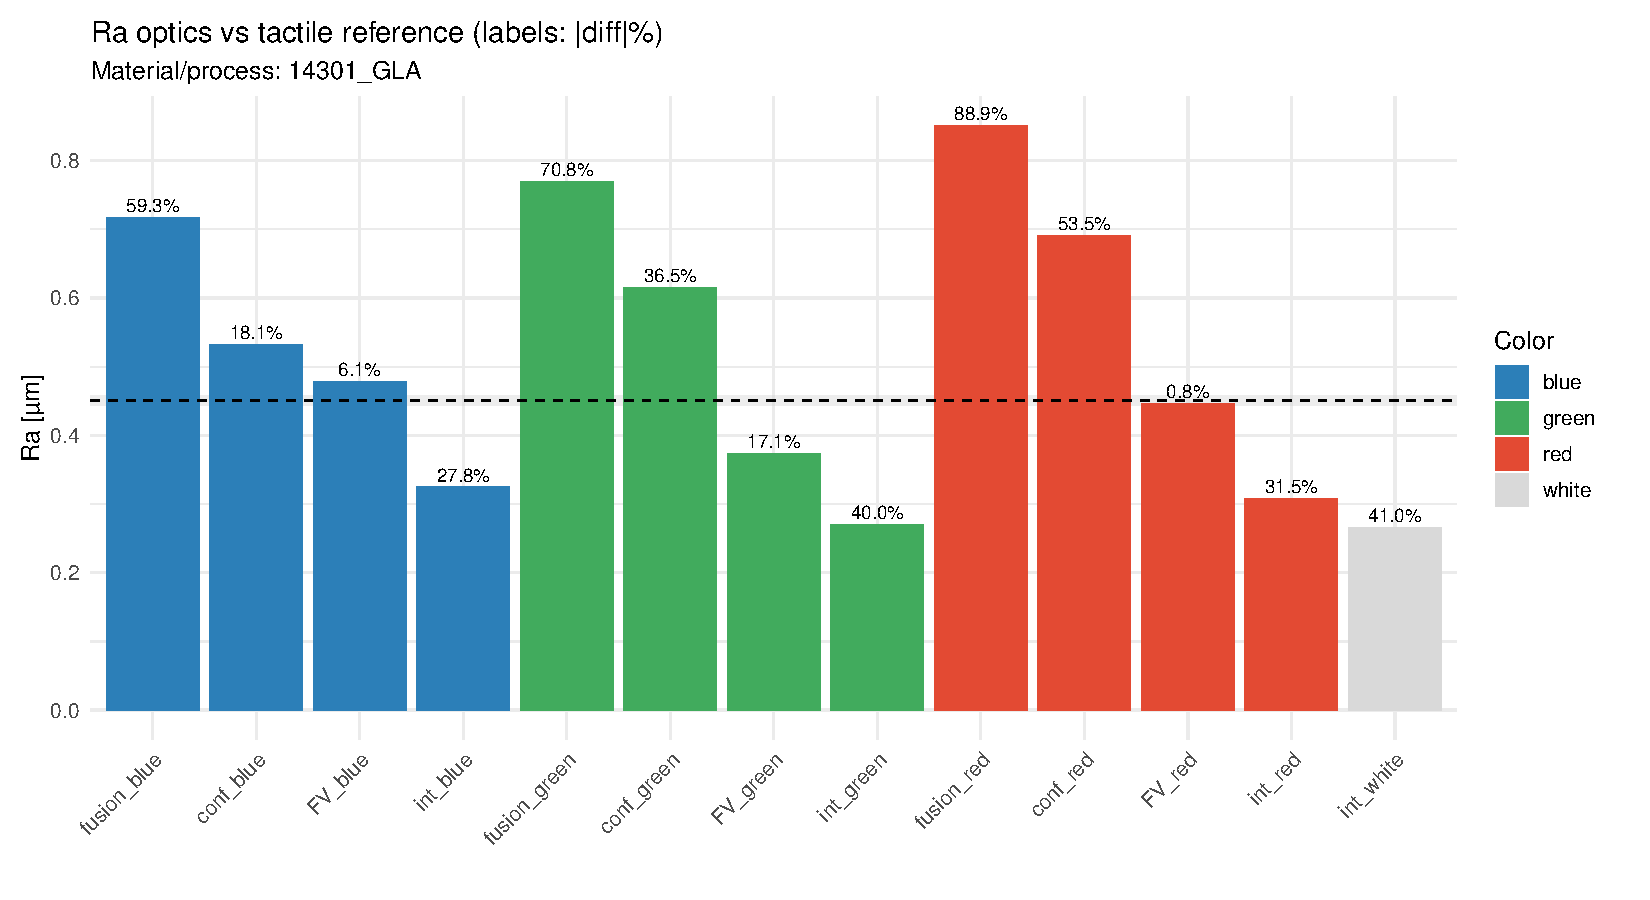
\includegraphics[width=\linewidth]{plots/ra_abs_14301_gla_optics_vs_tactile.pdf}
\end{minipage}
\begin{minipage}[t]{0.32\textwidth}\centering
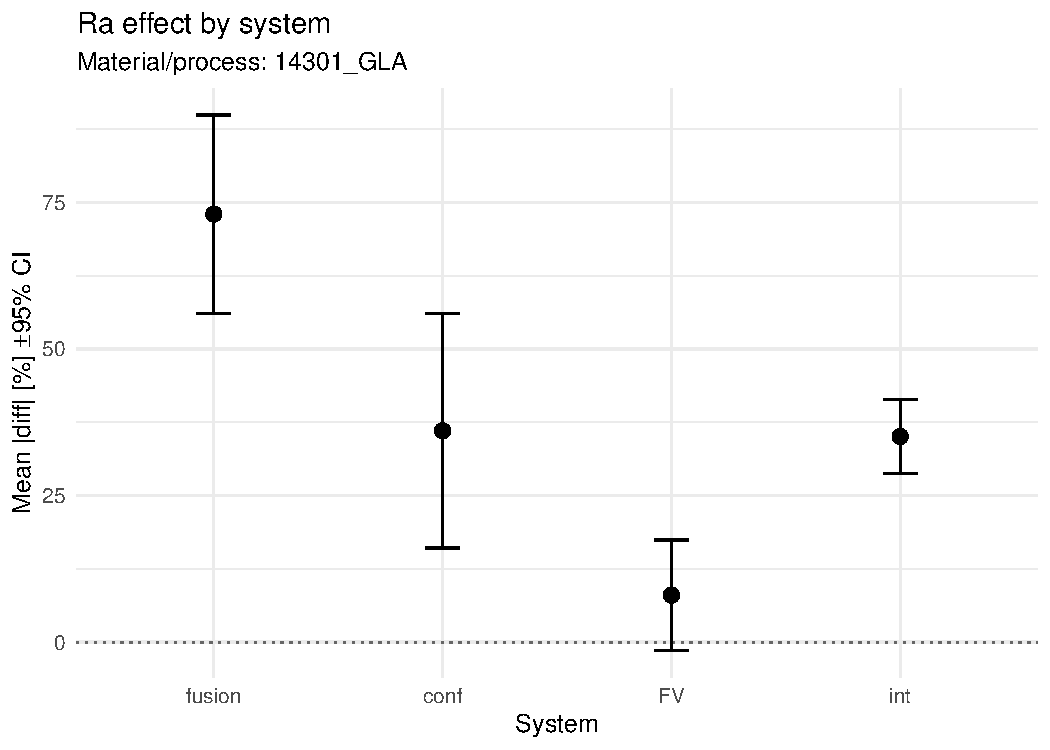
\includegraphics[width=\linewidth]{plots/ra_abs_14301_gla_effects_by_system.pdf}
\end{minipage}
\begin{minipage}[t]{0.32\textwidth}\centering
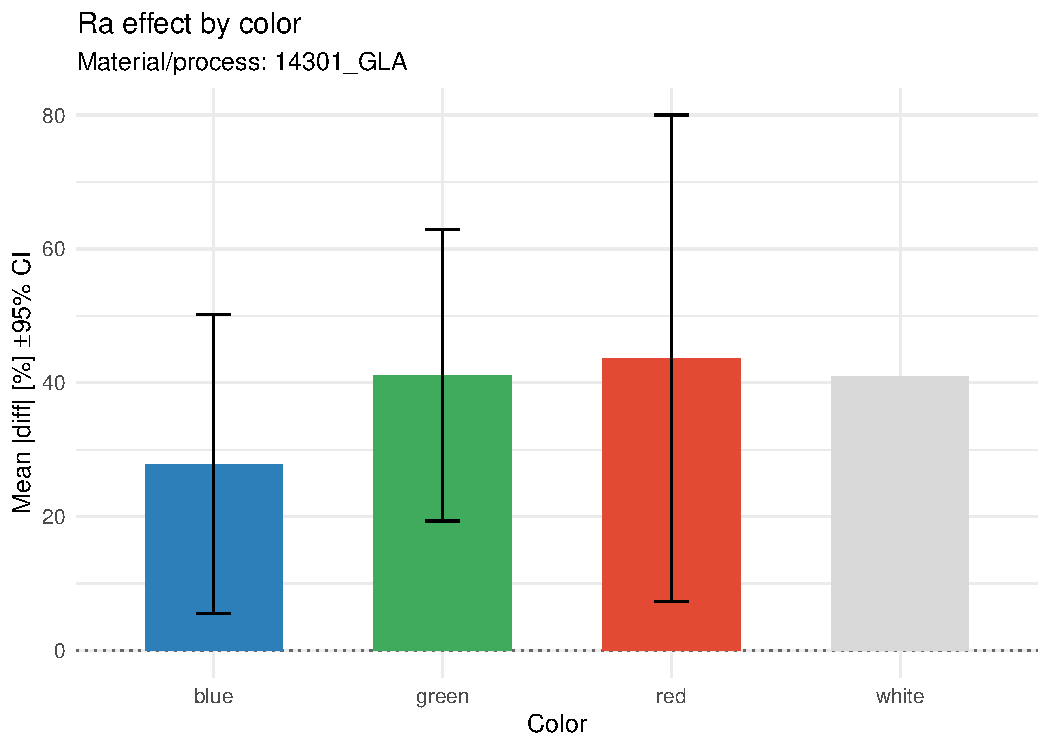
\includegraphics[width=\linewidth]{plots/ra_abs_14301_gla_effects_by_color.pdf}
\end{minipage}
\caption{RA — 14301\_gla — porównanie i efekty (|diff| \%)}
\end{figure}

\begin{figure}[H]\centering
\begin{minipage}[t]{0.32\textwidth}\centering
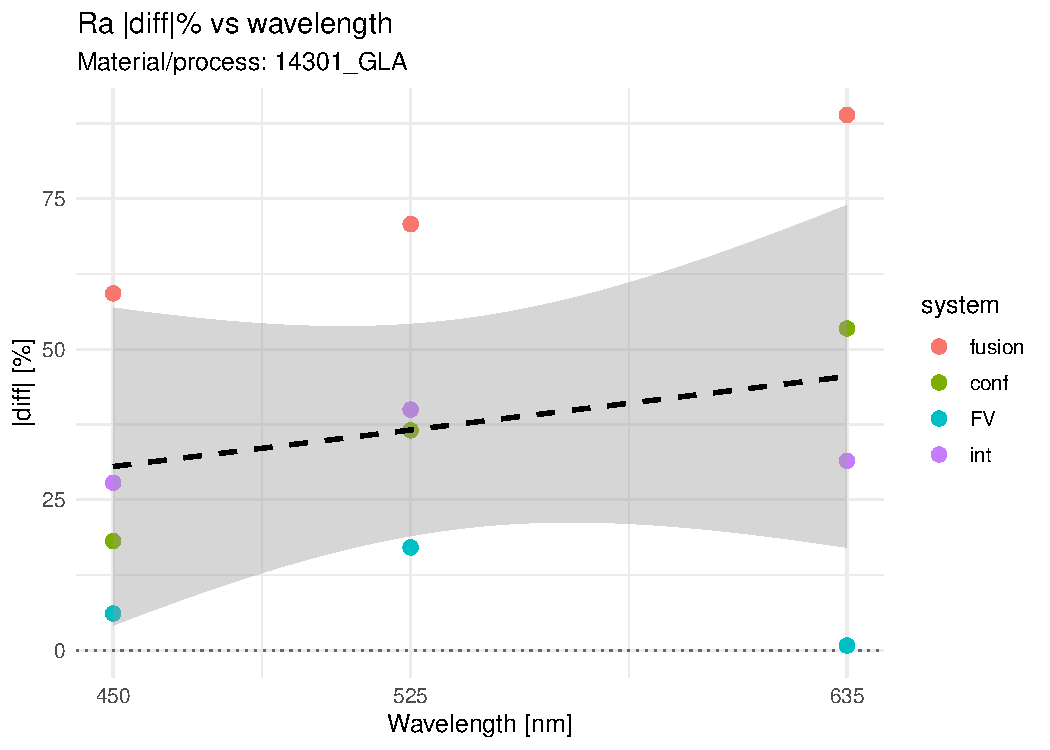
\includegraphics[width=\linewidth]{plots/ra_abs_14301_gla_diff_vs_wavelength.pdf}
\end{minipage}
\begin{minipage}[t]{0.32\textwidth}\centering
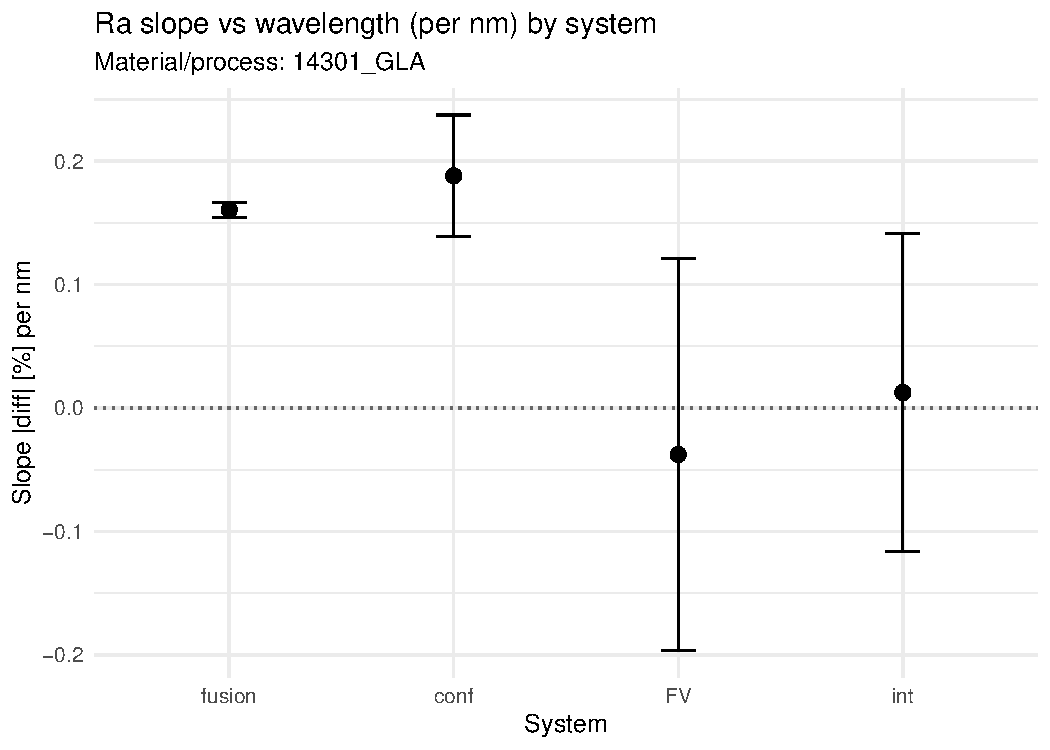
\includegraphics[width=\linewidth]{plots/ra_abs_14301_gla_slope_by_system_vs_nm.pdf}
\end{minipage}
\begin{minipage}[t]{0.32\textwidth}\centering
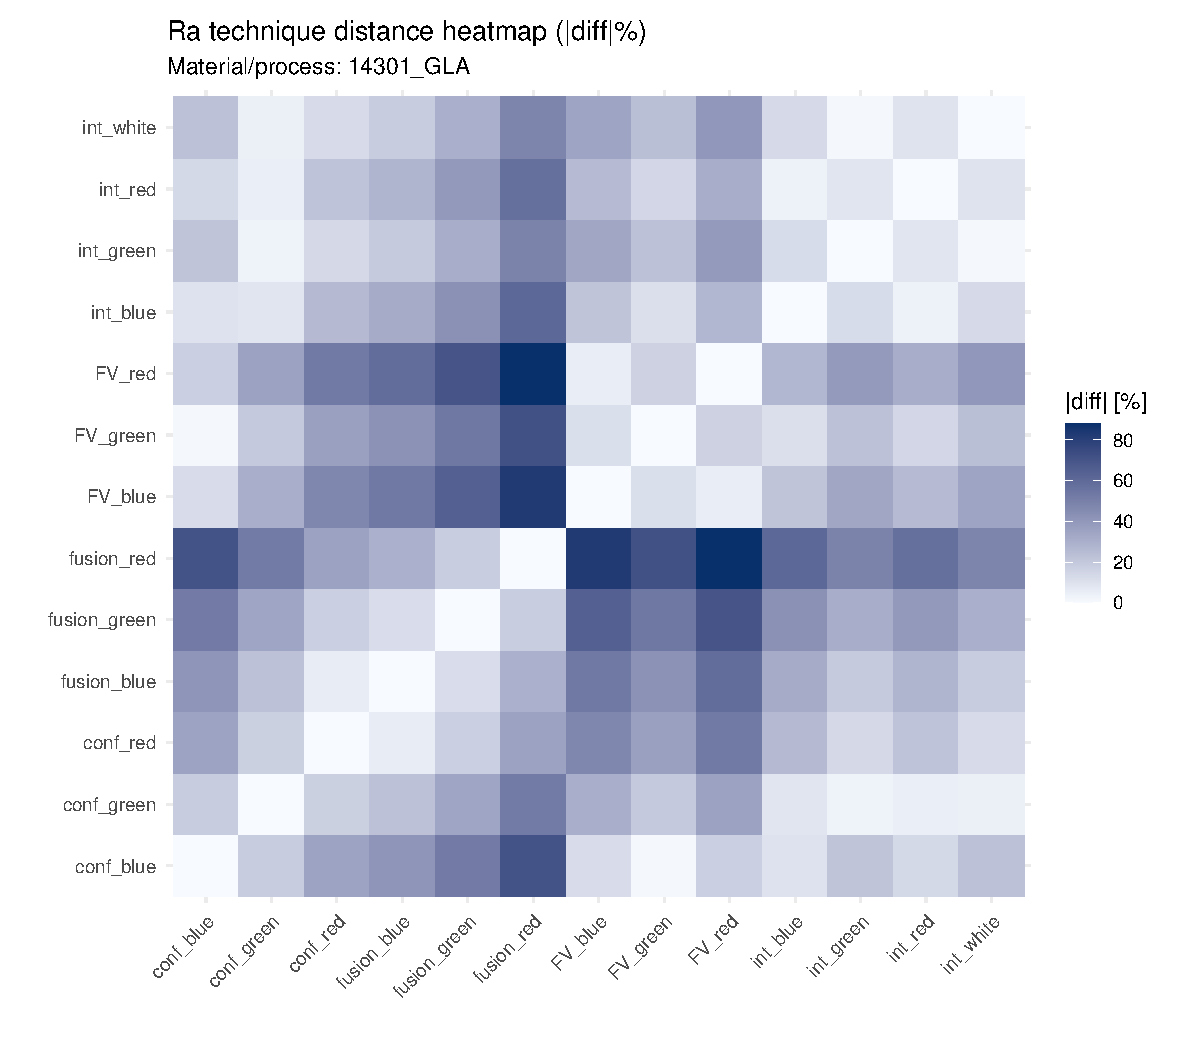
\includegraphics[width=\linewidth]{plots/ra_abs_14301_gla_tech_distance_heatmap.pdf}
\end{minipage}
\caption{RA — 14301\_gla — wavelength, nachylenia, odległości technik}
\end{figure}

\begin{figure}[H]\centering
\begin{minipage}[t]{0.32\textwidth}\centering
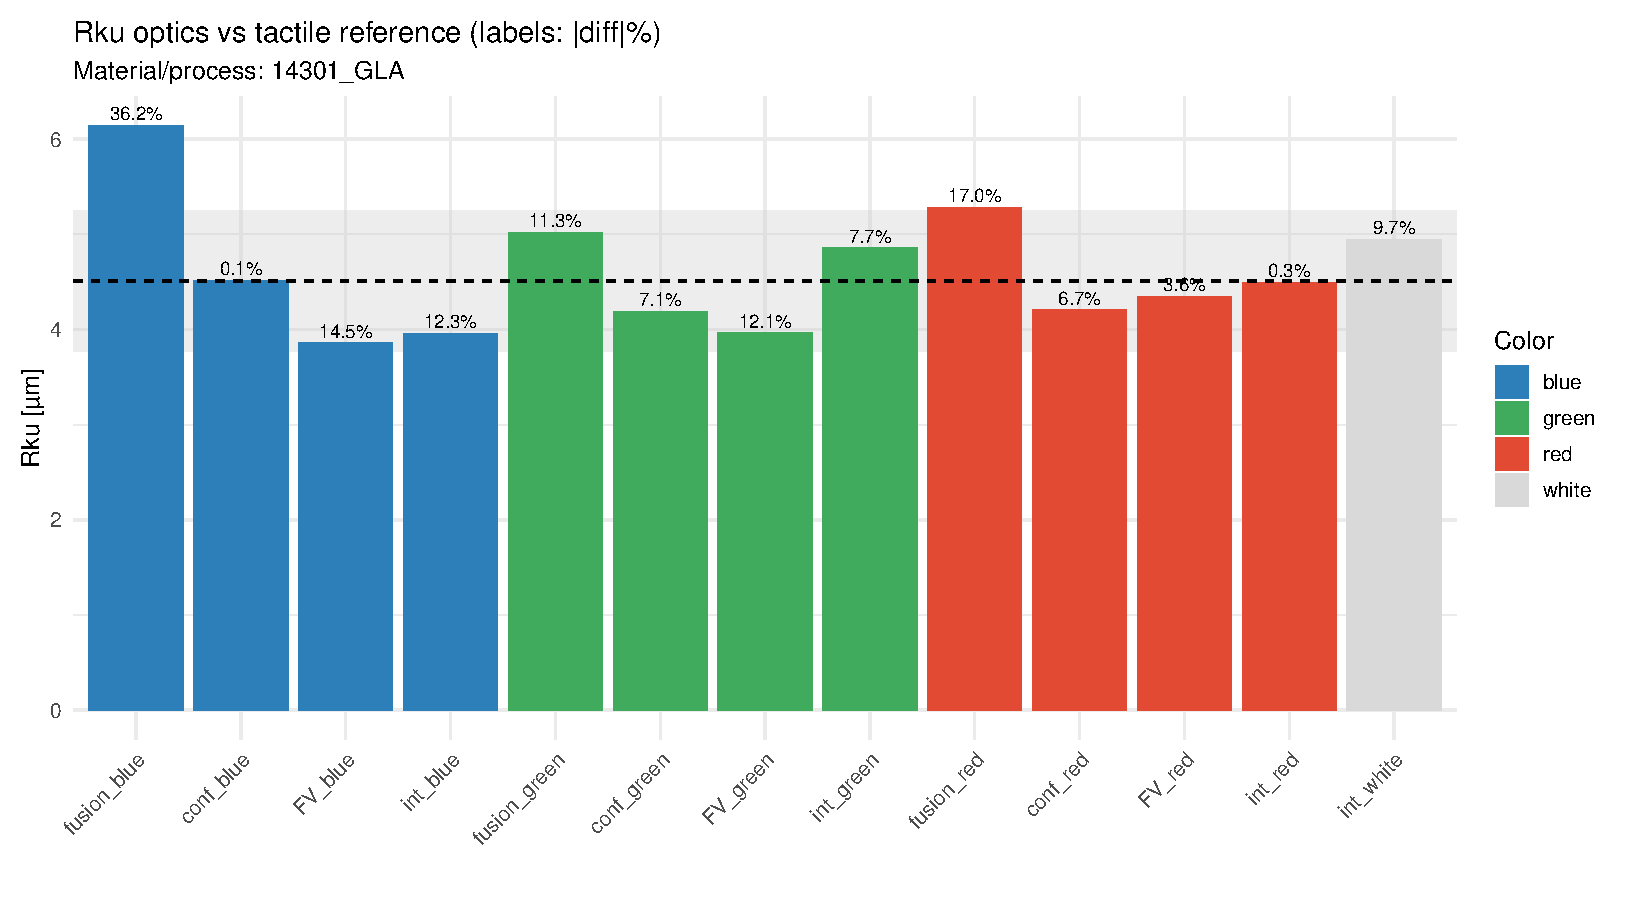
\includegraphics[width=\linewidth]{plots/rku_abs_14301_gla_optics_vs_tactile.pdf}
\end{minipage}
\begin{minipage}[t]{0.32\textwidth}\centering
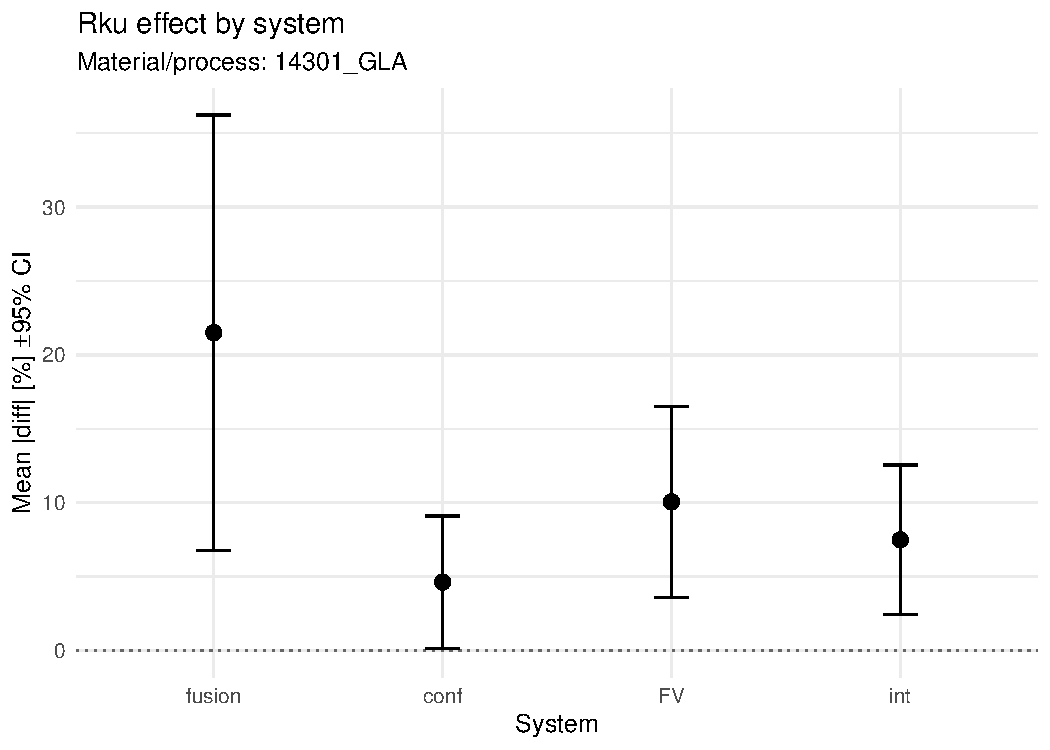
\includegraphics[width=\linewidth]{plots/rku_abs_14301_gla_effects_by_system.pdf}
\end{minipage}
\begin{minipage}[t]{0.32\textwidth}\centering
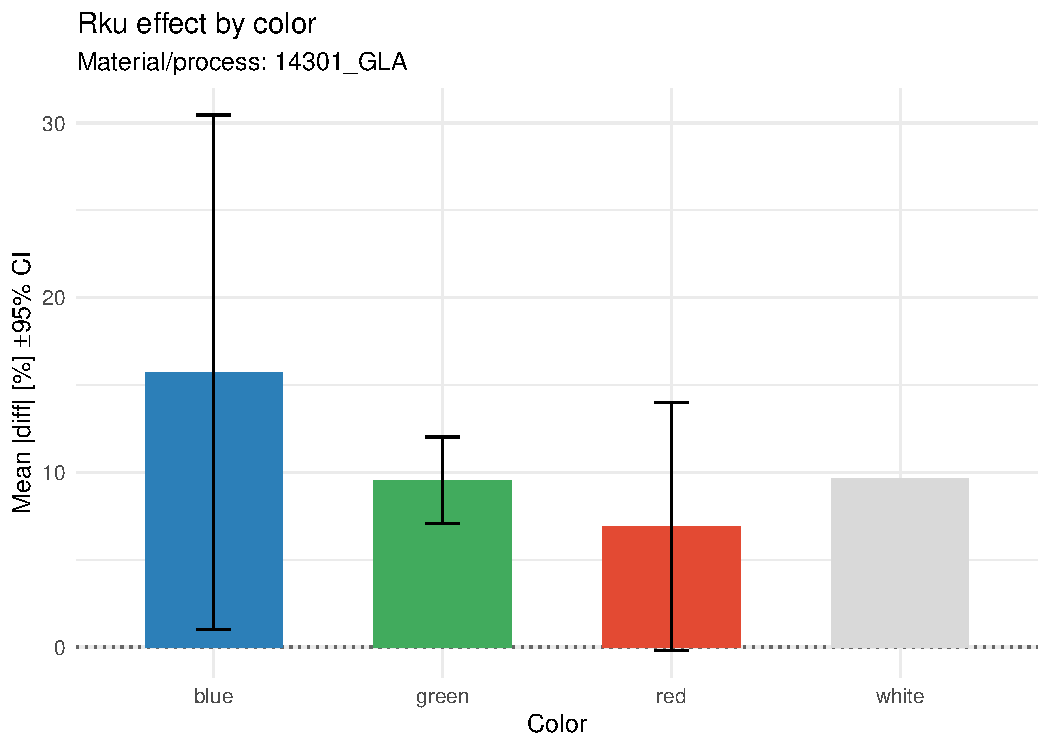
\includegraphics[width=\linewidth]{plots/rku_abs_14301_gla_effects_by_color.pdf}
\end{minipage}
\caption{RKU — 14301\_gla — porównanie i efekty (|diff| \%)}
\end{figure}

\begin{figure}[H]\centering
\begin{minipage}[t]{0.32\textwidth}\centering
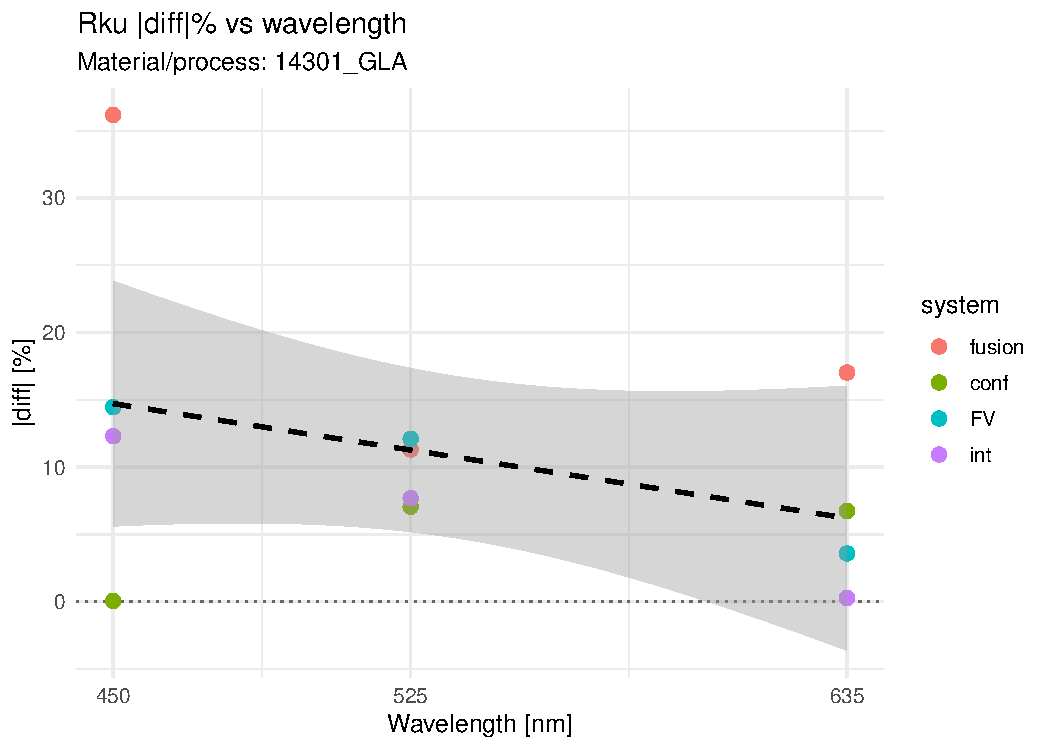
\includegraphics[width=\linewidth]{plots/rku_abs_14301_gla_diff_vs_wavelength.pdf}
\end{minipage}
\begin{minipage}[t]{0.32\textwidth}\centering
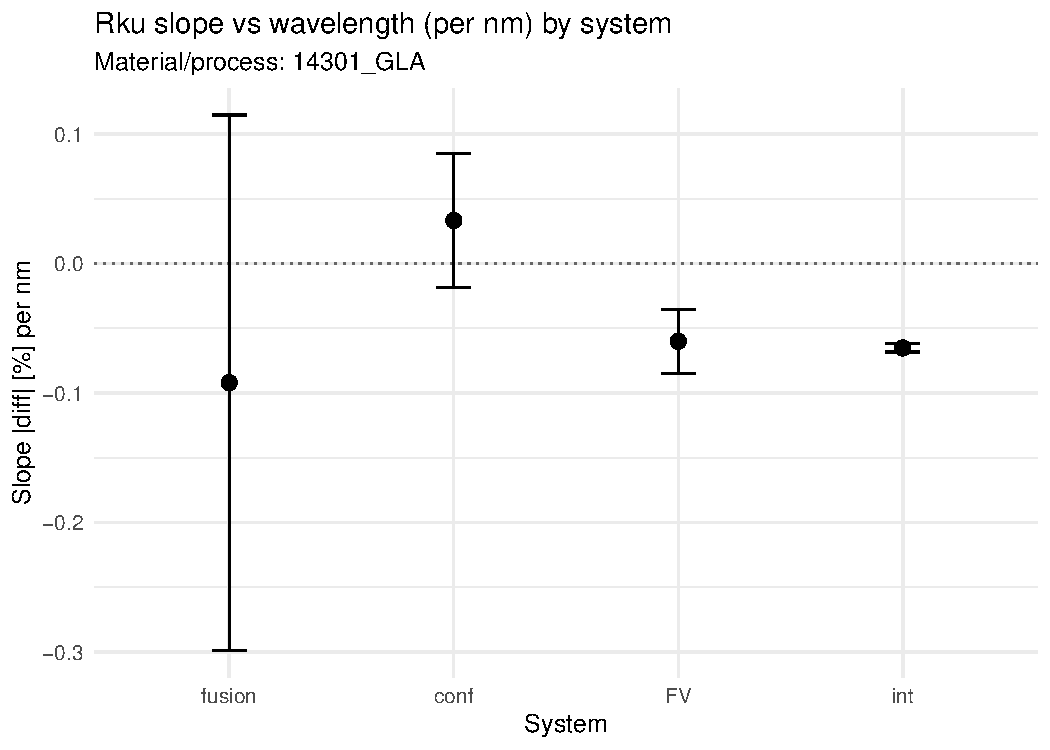
\includegraphics[width=\linewidth]{plots/rku_abs_14301_gla_slope_by_system_vs_nm.pdf}
\end{minipage}
\begin{minipage}[t]{0.32\textwidth}\centering
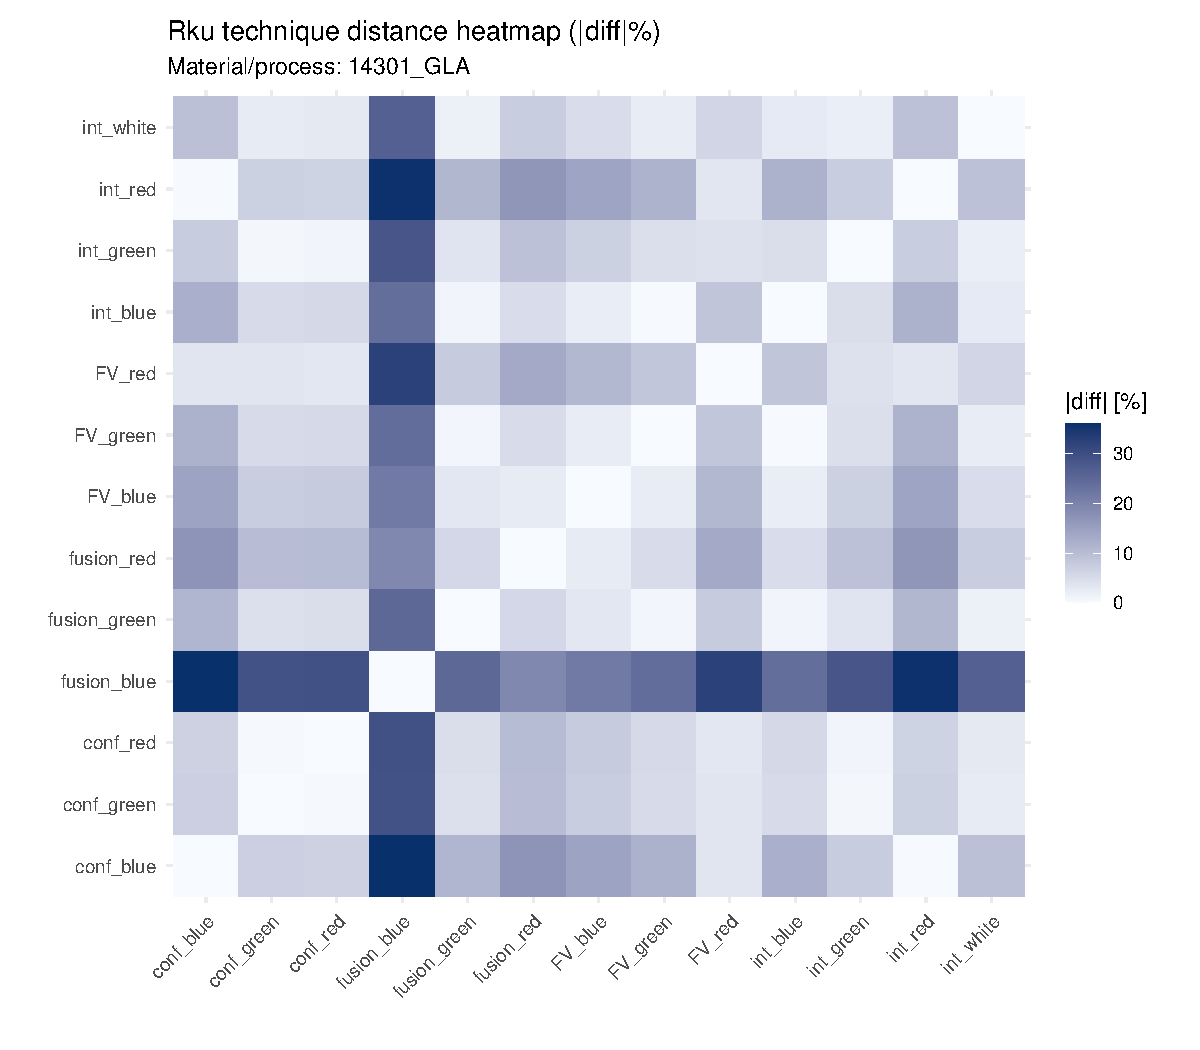
\includegraphics[width=\linewidth]{plots/rku_abs_14301_gla_tech_distance_heatmap.pdf}
\end{minipage}
\caption{RKU — 14301\_gla — wavelength, nachylenia, odległości technik}
\end{figure}

\begin{figure}[H]\centering
\begin{minipage}[t]{0.32\textwidth}\centering
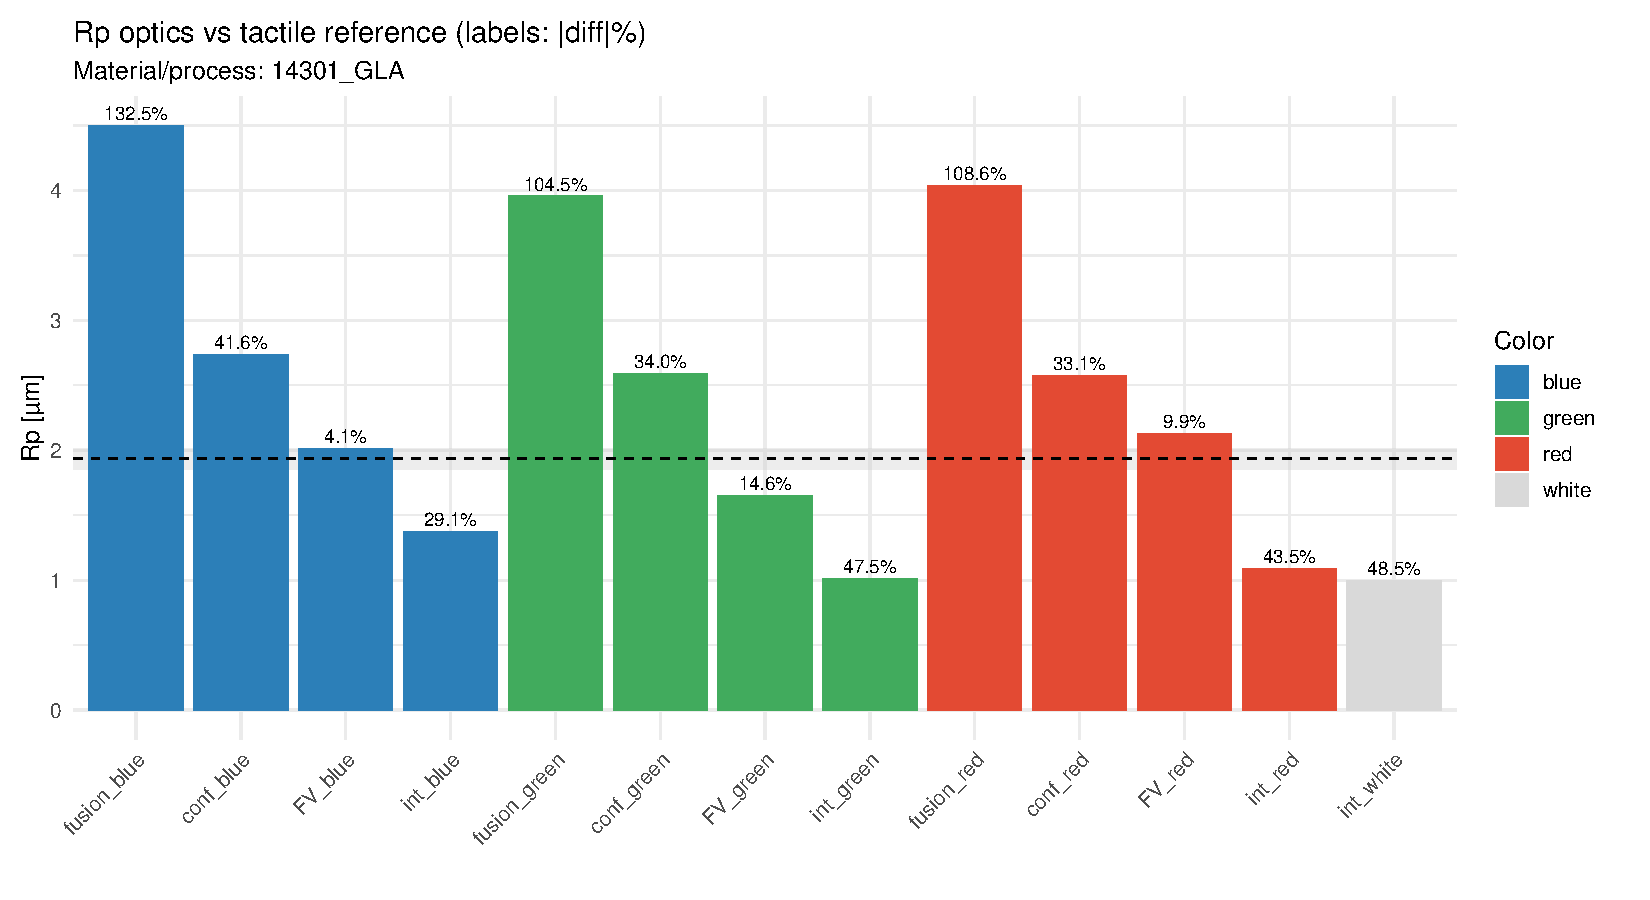
\includegraphics[width=\linewidth]{plots/rp_abs_14301_gla_optics_vs_tactile.pdf}
\end{minipage}
\begin{minipage}[t]{0.32\textwidth}\centering
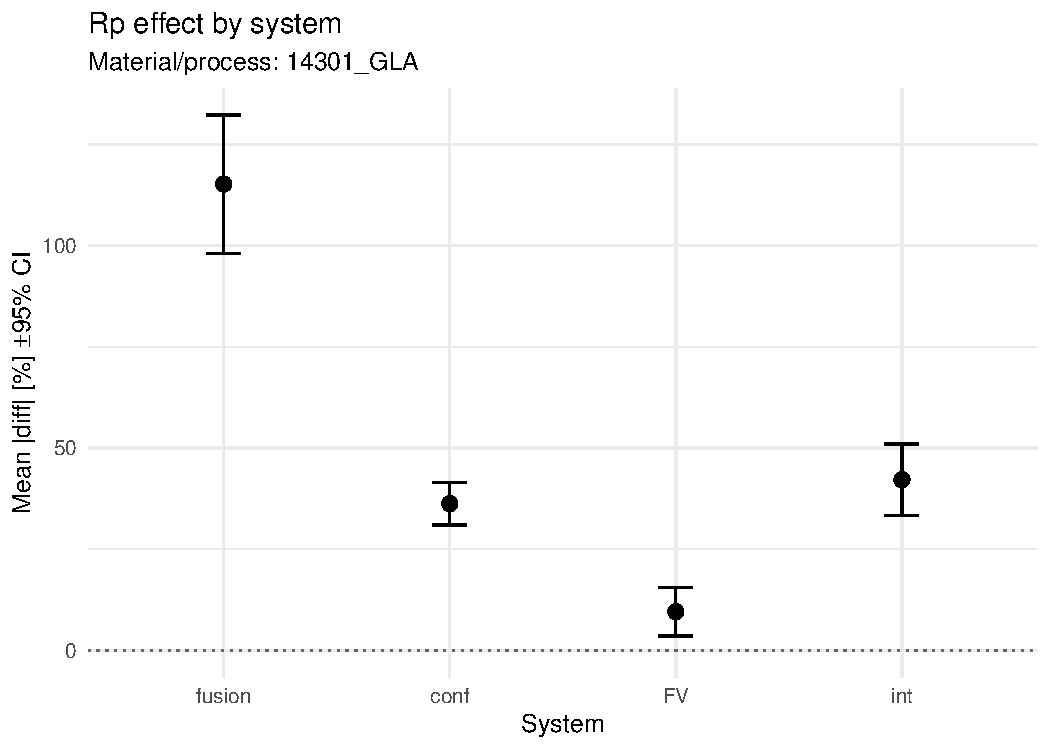
\includegraphics[width=\linewidth]{plots/rp_abs_14301_gla_effects_by_system.pdf}
\end{minipage}
\begin{minipage}[t]{0.32\textwidth}\centering
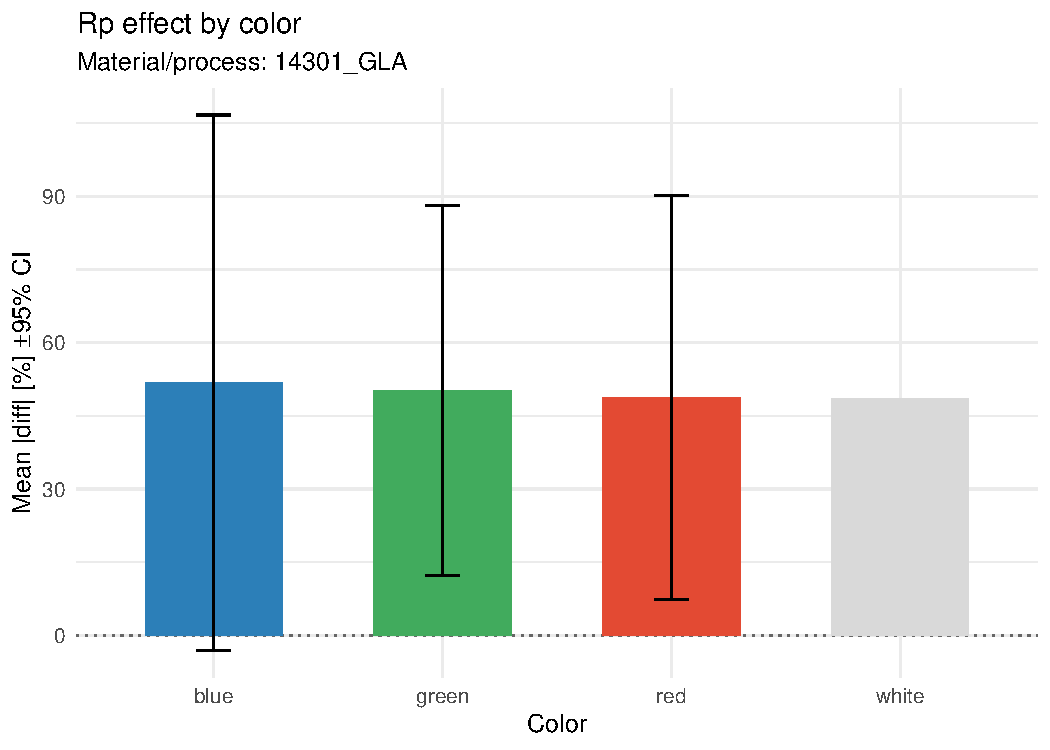
\includegraphics[width=\linewidth]{plots/rp_abs_14301_gla_effects_by_color.pdf}
\end{minipage}
\caption{RP — 14301\_gla — porównanie i efekty (|diff| \%)}
\end{figure}

\begin{figure}[H]\centering
\begin{minipage}[t]{0.32\textwidth}\centering
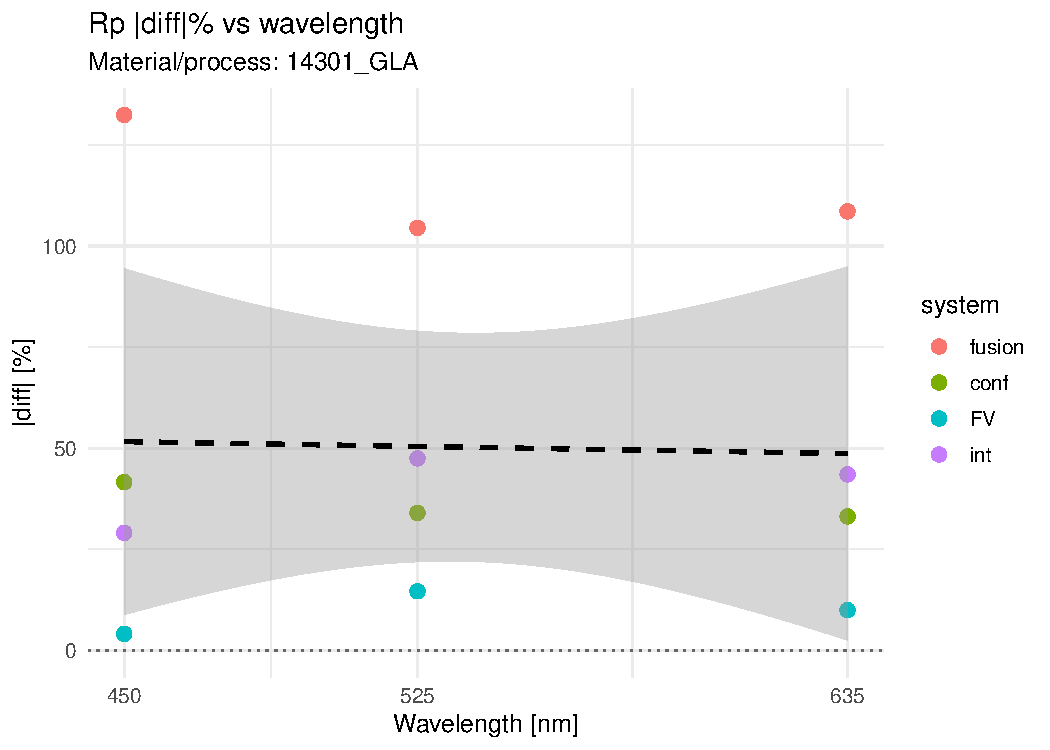
\includegraphics[width=\linewidth]{plots/rp_abs_14301_gla_diff_vs_wavelength.pdf}
\end{minipage}
\begin{minipage}[t]{0.32\textwidth}\centering
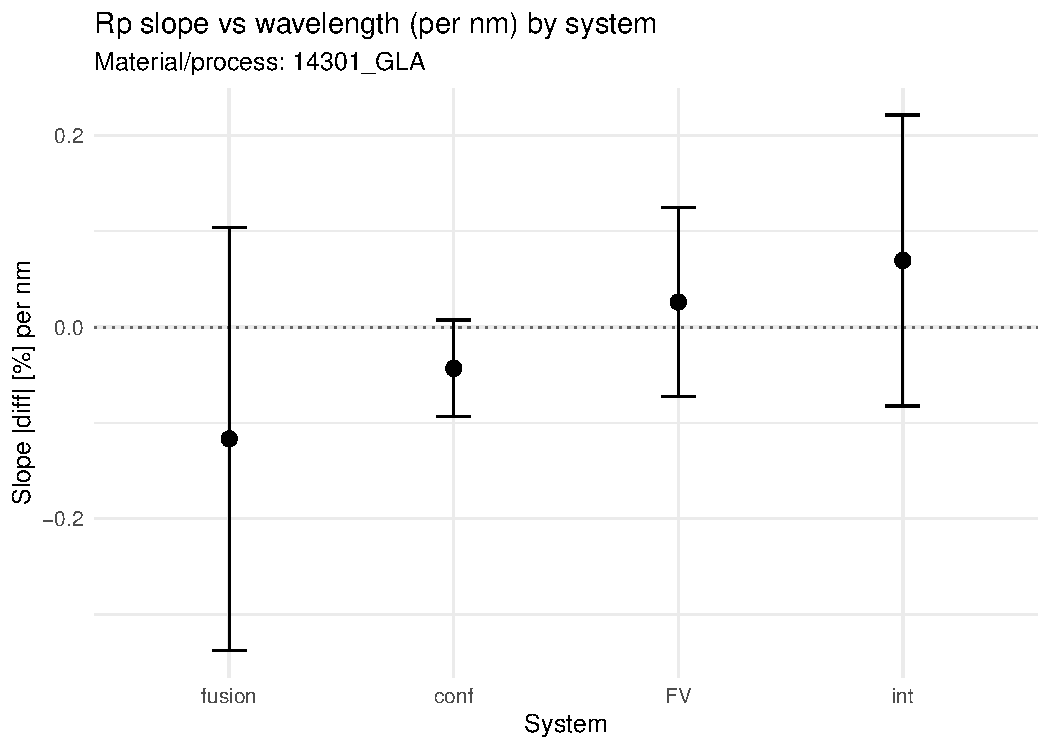
\includegraphics[width=\linewidth]{plots/rp_abs_14301_gla_slope_by_system_vs_nm.pdf}
\end{minipage}
\begin{minipage}[t]{0.32\textwidth}\centering
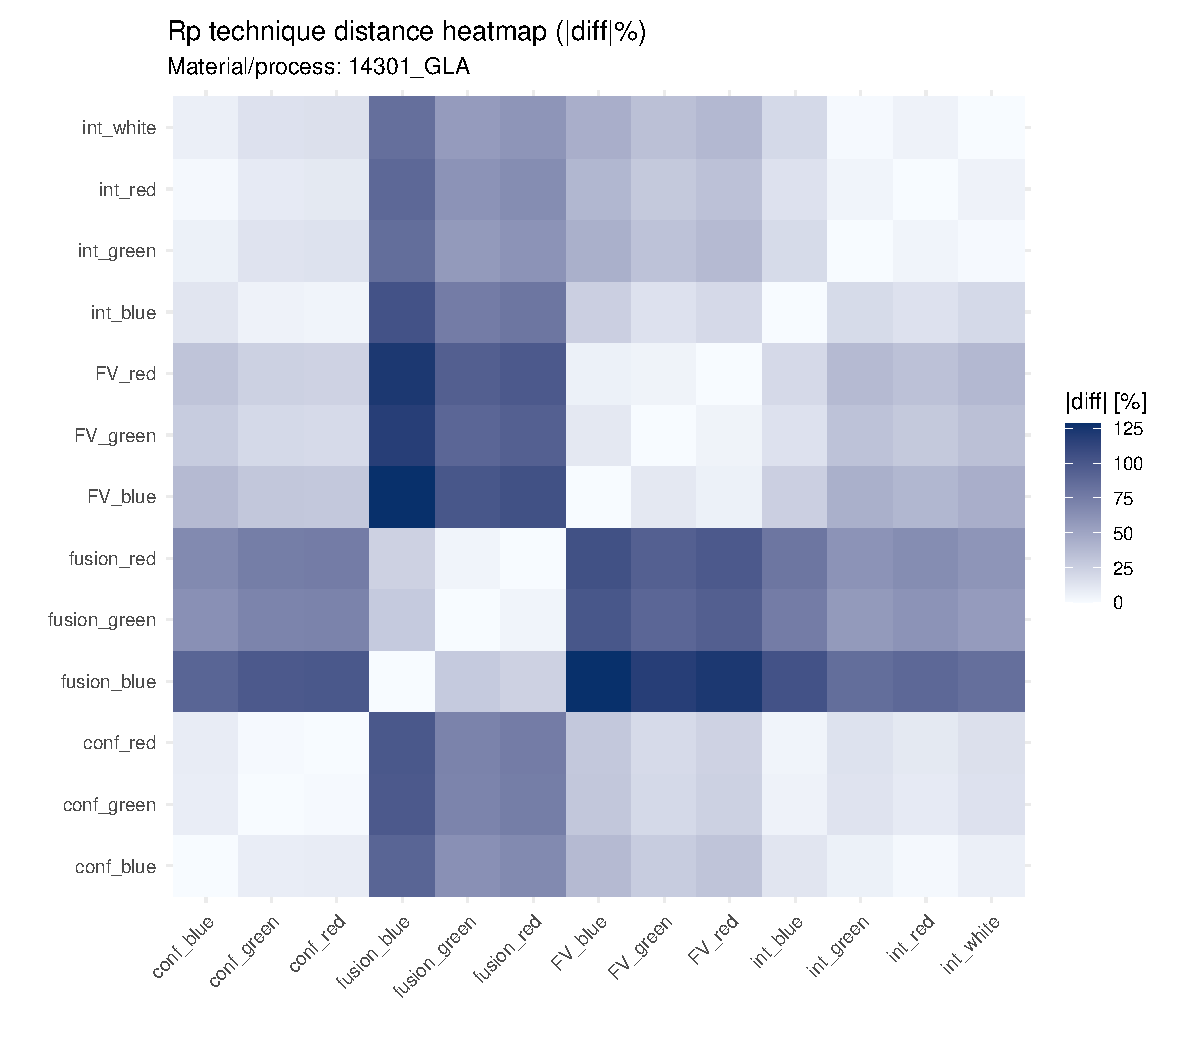
\includegraphics[width=\linewidth]{plots/rp_abs_14301_gla_tech_distance_heatmap.pdf}
\end{minipage}
\caption{RP — 14301\_gla — wavelength, nachylenia, odległości technik}
\end{figure}

\begin{figure}[H]\centering
\begin{minipage}[t]{0.32\textwidth}\centering
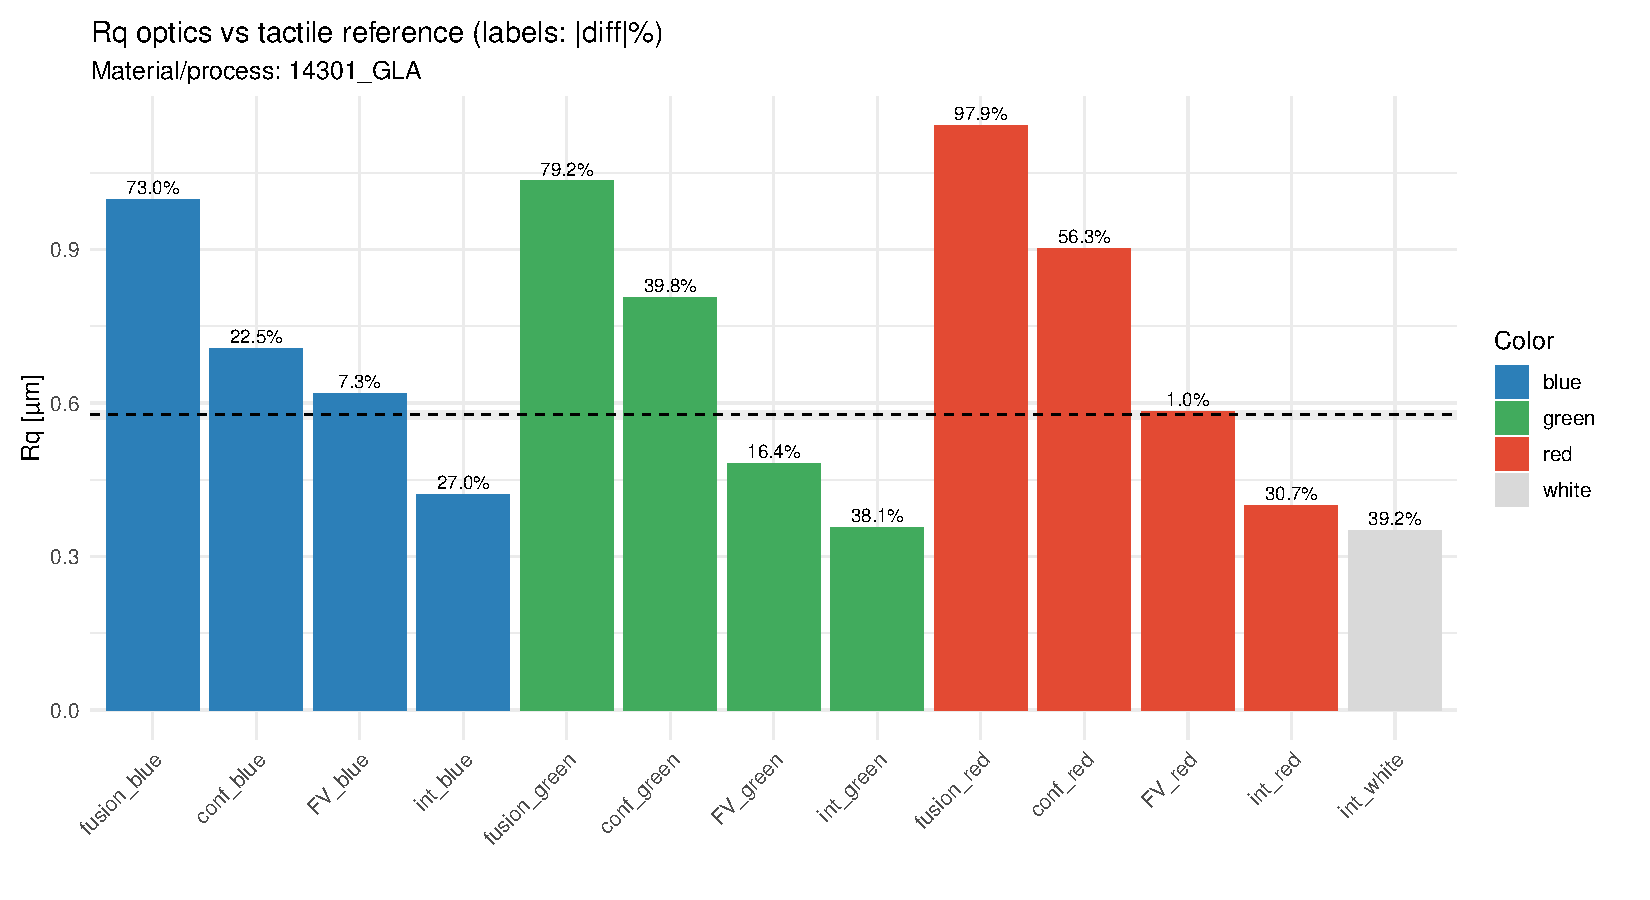
\includegraphics[width=\linewidth]{plots/rq_abs_14301_gla_optics_vs_tactile.pdf}
\end{minipage}
\begin{minipage}[t]{0.32\textwidth}\centering
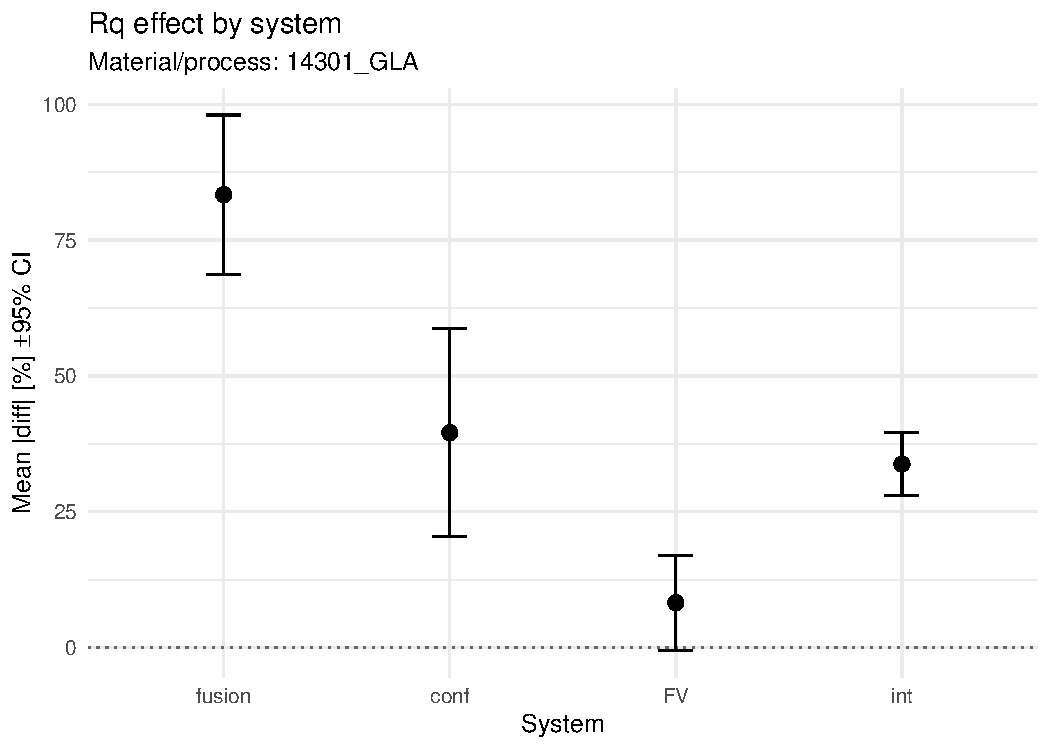
\includegraphics[width=\linewidth]{plots/rq_abs_14301_gla_effects_by_system.pdf}
\end{minipage}
\begin{minipage}[t]{0.32\textwidth}\centering
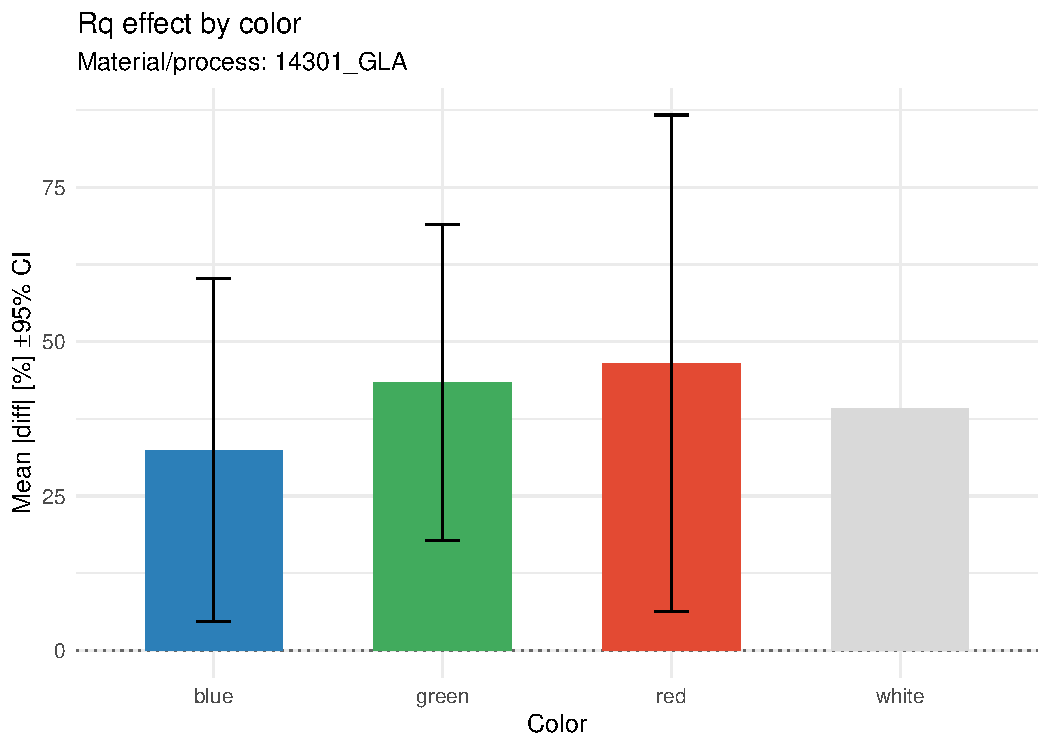
\includegraphics[width=\linewidth]{plots/rq_abs_14301_gla_effects_by_color.pdf}
\end{minipage}
\caption{RQ — 14301\_gla — porównanie i efekty (|diff| \%)}
\end{figure}

\begin{figure}[H]\centering
\begin{minipage}[t]{0.32\textwidth}\centering
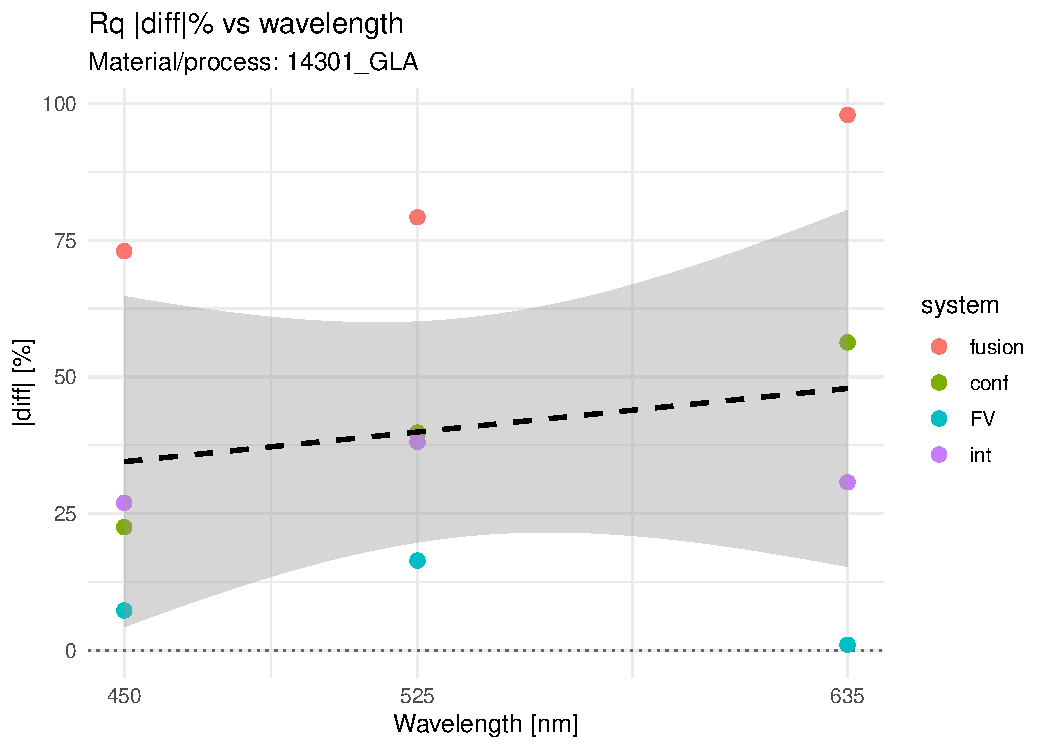
\includegraphics[width=\linewidth]{plots/rq_abs_14301_gla_diff_vs_wavelength.pdf}
\end{minipage}
\begin{minipage}[t]{0.32\textwidth}\centering
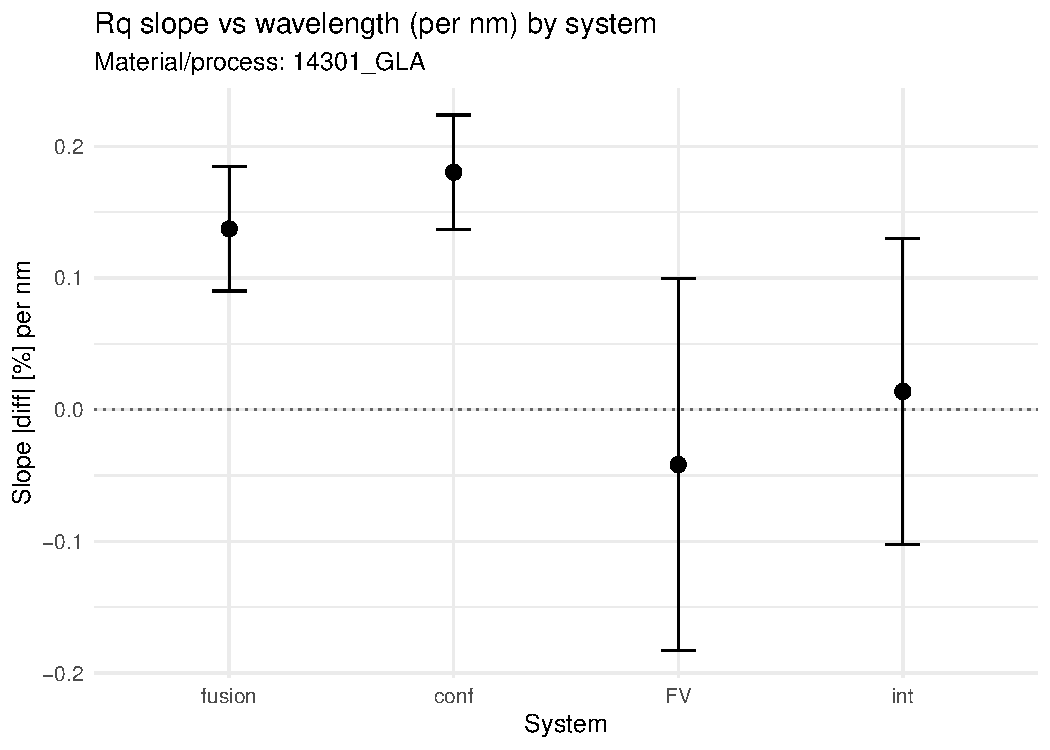
\includegraphics[width=\linewidth]{plots/rq_abs_14301_gla_slope_by_system_vs_nm.pdf}
\end{minipage}
\begin{minipage}[t]{0.32\textwidth}\centering
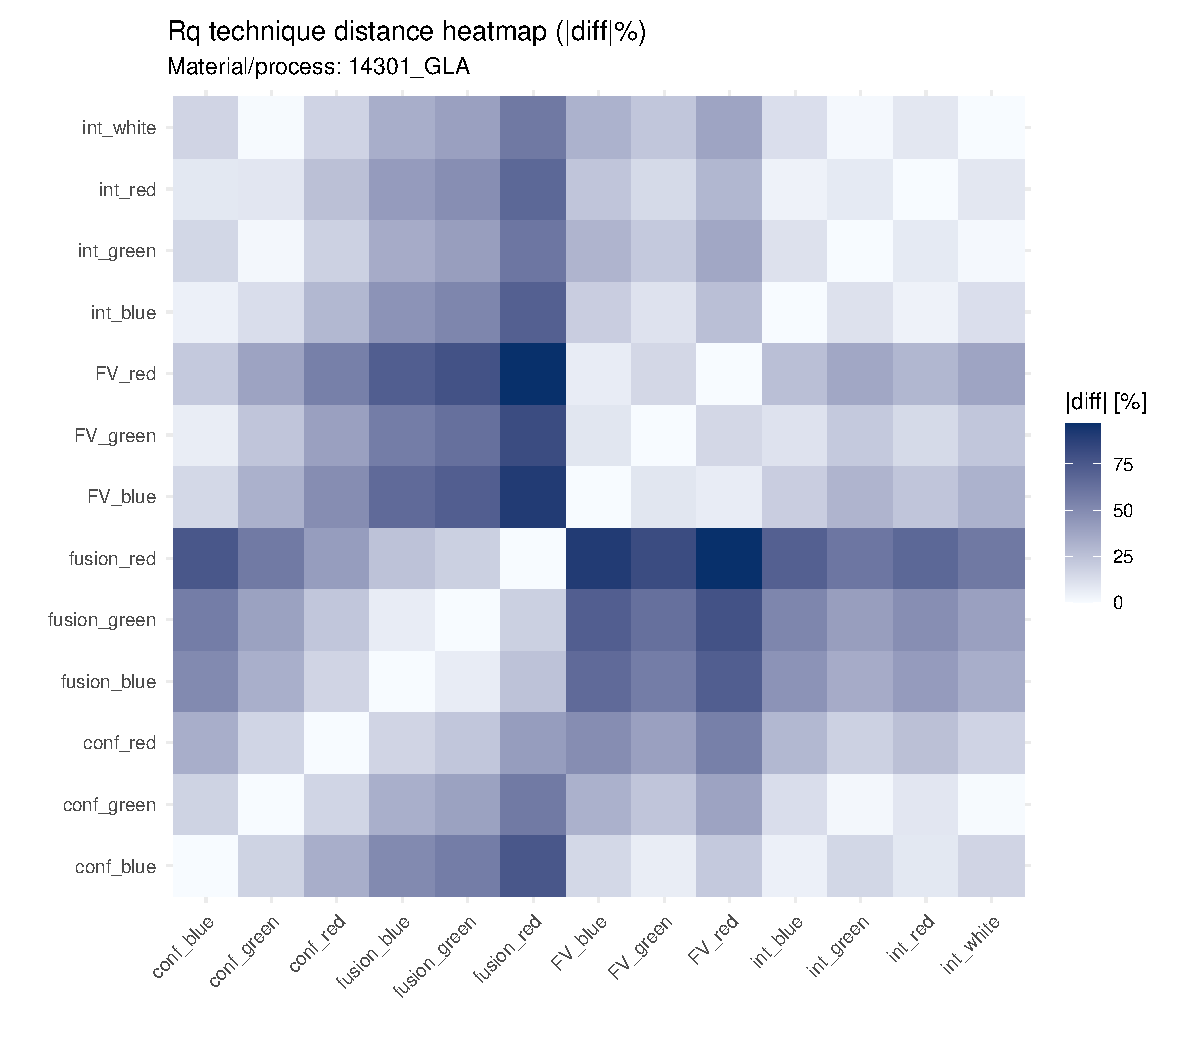
\includegraphics[width=\linewidth]{plots/rq_abs_14301_gla_tech_distance_heatmap.pdf}
\end{minipage}
\caption{RQ — 14301\_gla — wavelength, nachylenia, odległości technik}
\end{figure}

\begin{figure}[H]\centering
\begin{minipage}[t]{0.32\textwidth}\centering
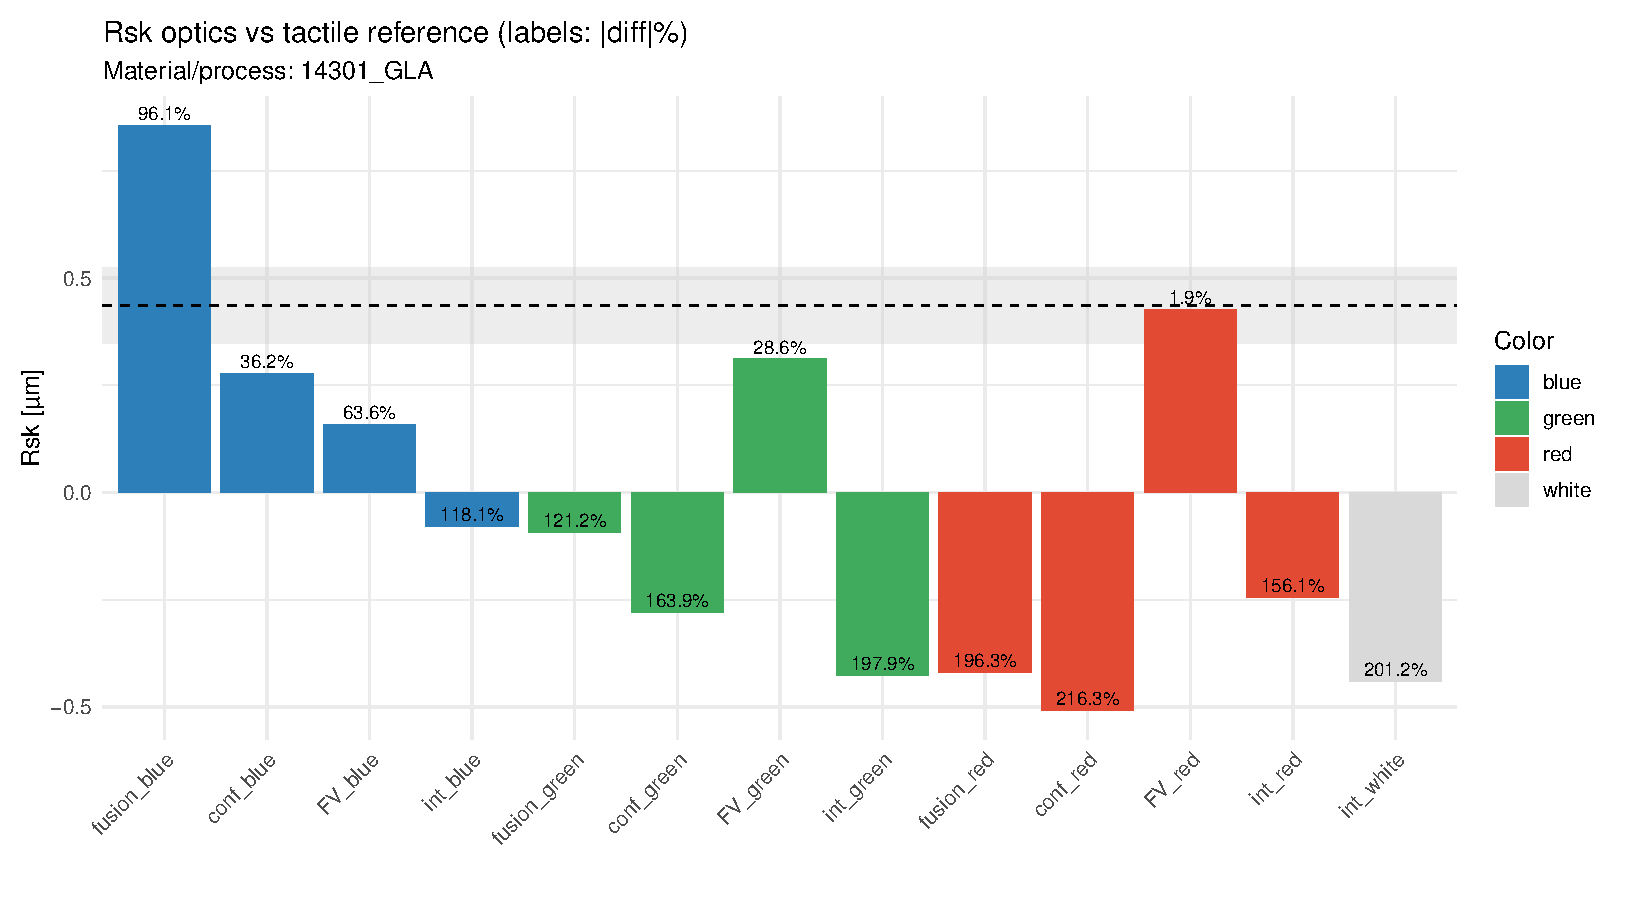
\includegraphics[width=\linewidth]{plots/rsk_abs_14301_gla_optics_vs_tactile.pdf}
\end{minipage}
\begin{minipage}[t]{0.32\textwidth}\centering
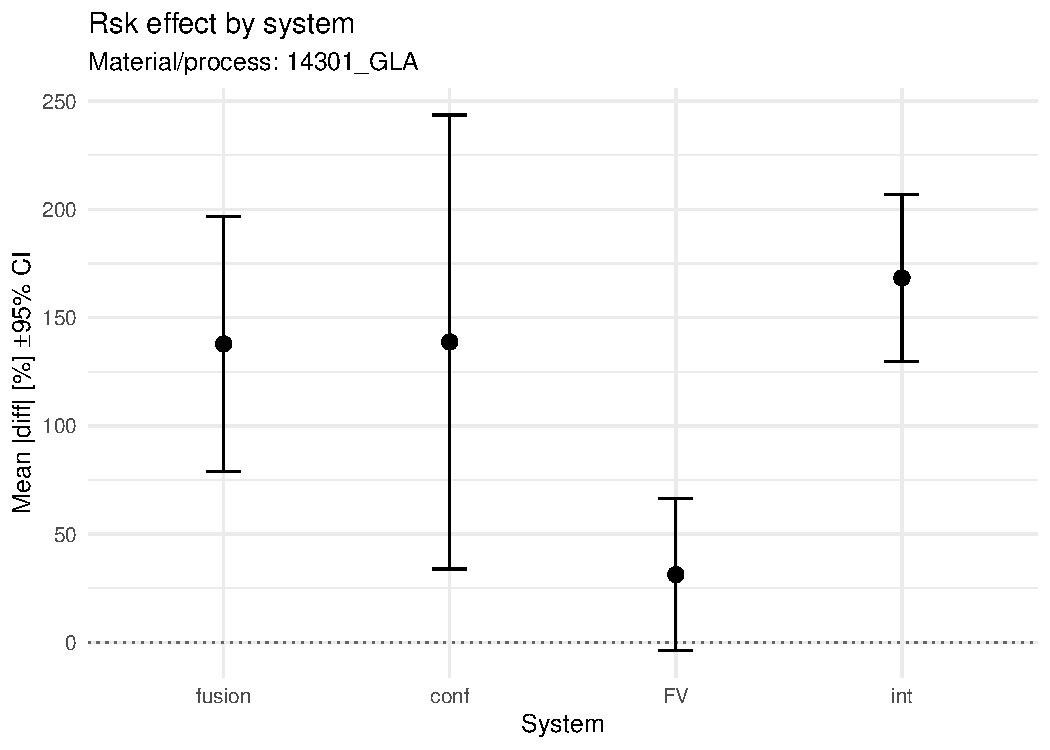
\includegraphics[width=\linewidth]{plots/rsk_abs_14301_gla_effects_by_system.pdf}
\end{minipage}
\begin{minipage}[t]{0.32\textwidth}\centering
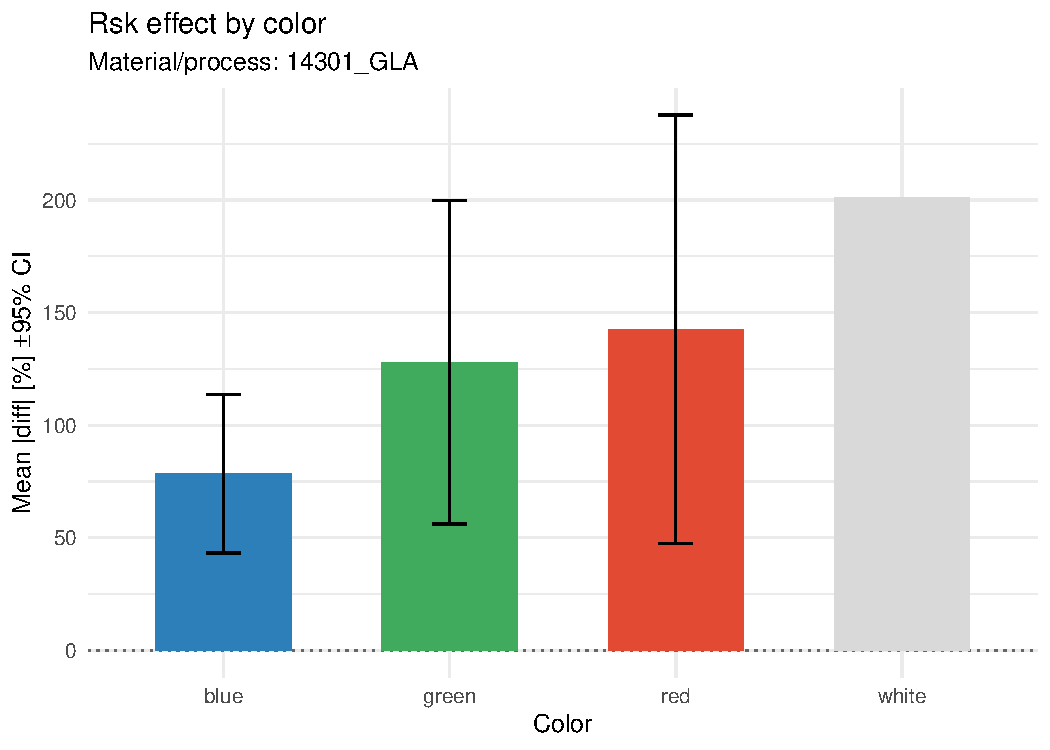
\includegraphics[width=\linewidth]{plots/rsk_abs_14301_gla_effects_by_color.pdf}
\end{minipage}
\caption{RSK — 14301\_gla — porównanie i efekty (|diff| \%)}
\end{figure}

\begin{figure}[H]\centering
\begin{minipage}[t]{0.32\textwidth}\centering
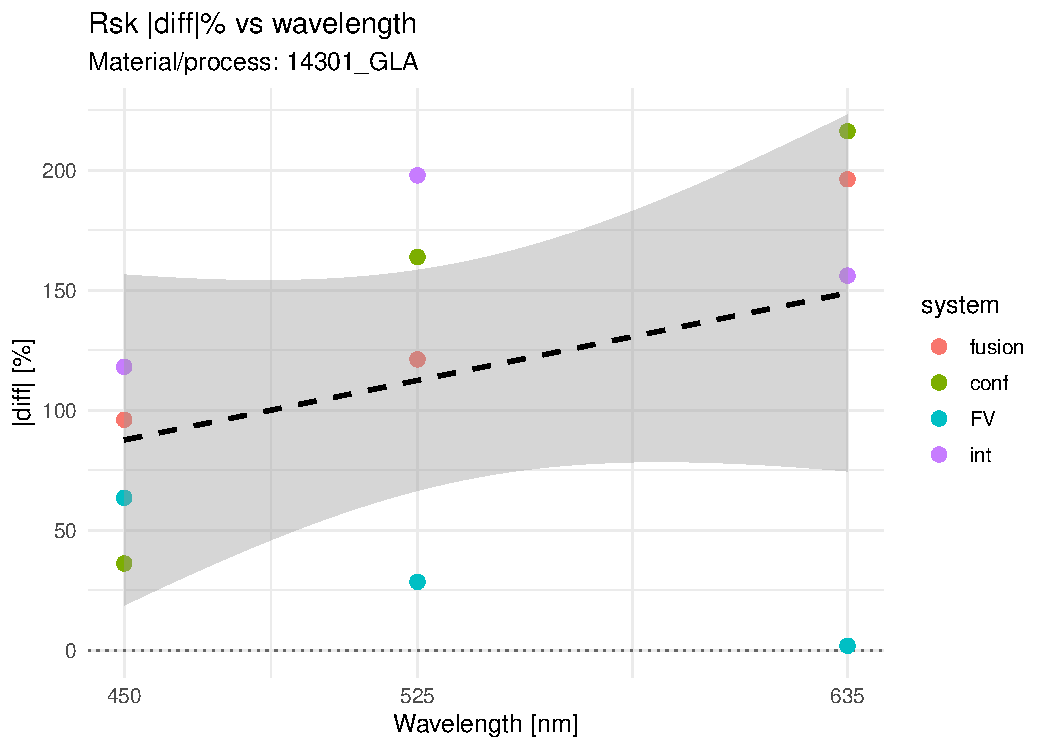
\includegraphics[width=\linewidth]{plots/rsk_abs_14301_gla_diff_vs_wavelength.pdf}
\end{minipage}
\begin{minipage}[t]{0.32\textwidth}\centering
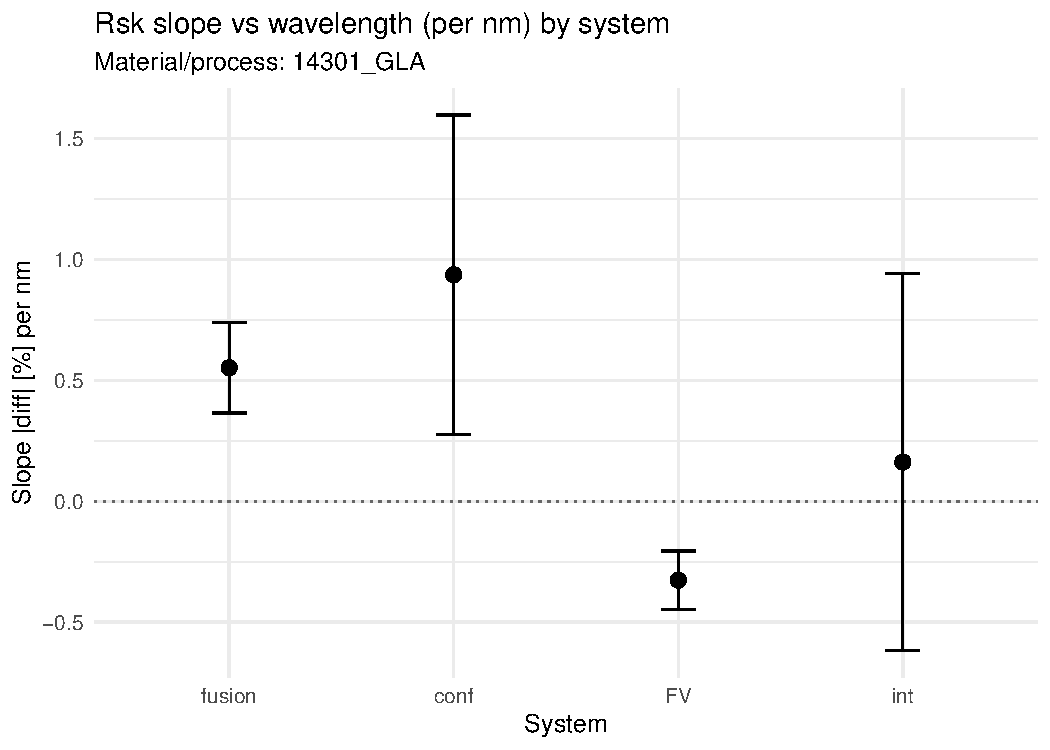
\includegraphics[width=\linewidth]{plots/rsk_abs_14301_gla_slope_by_system_vs_nm.pdf}
\end{minipage}
\begin{minipage}[t]{0.32\textwidth}\centering
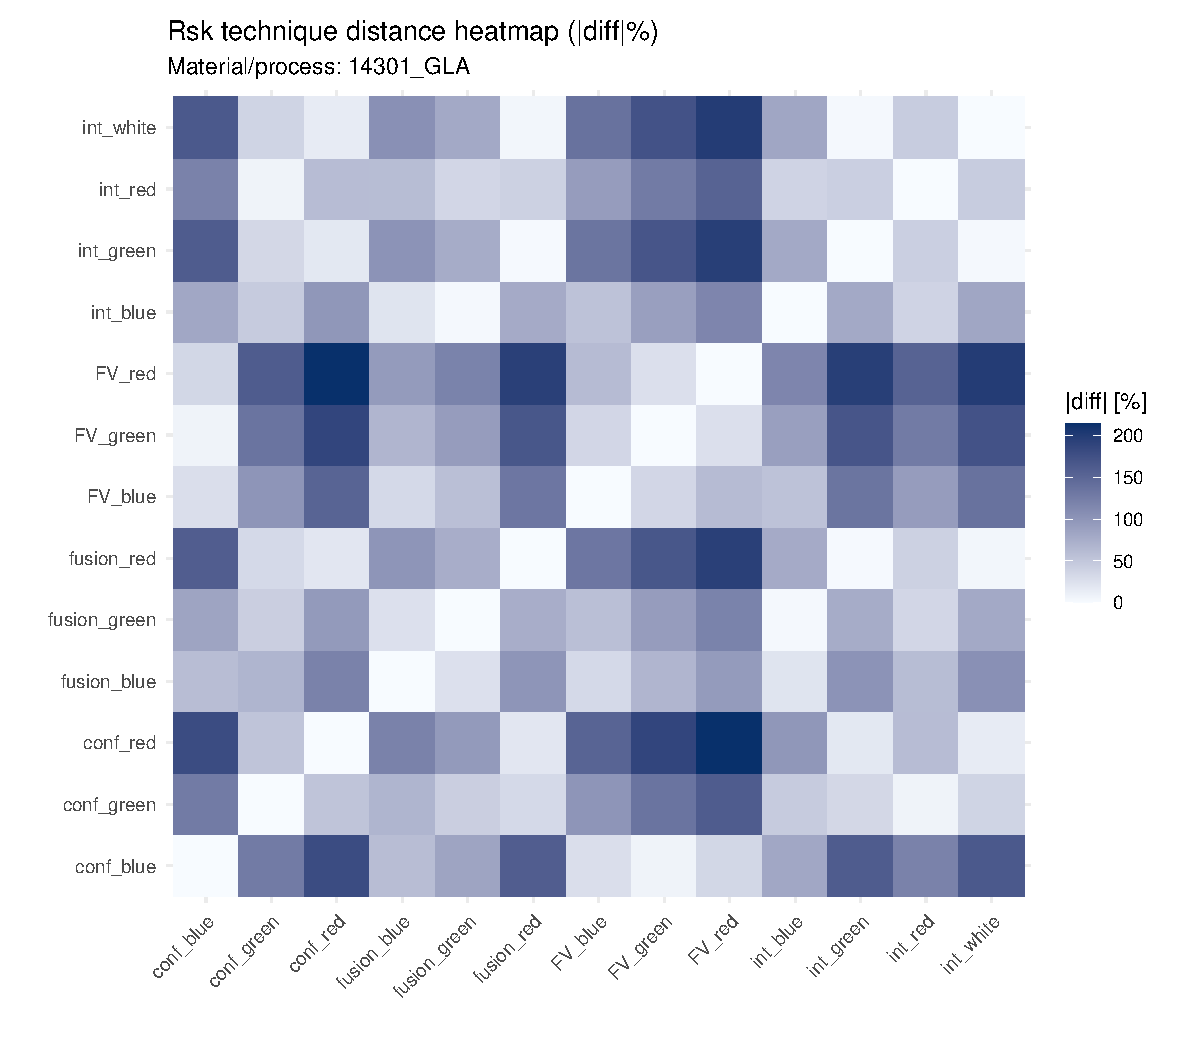
\includegraphics[width=\linewidth]{plots/rsk_abs_14301_gla_tech_distance_heatmap.pdf}
\end{minipage}
\caption{RSK — 14301\_gla — wavelength, nachylenia, odległości technik}
\end{figure}

\begin{figure}[H]\centering
\begin{minipage}[t]{0.32\textwidth}\centering
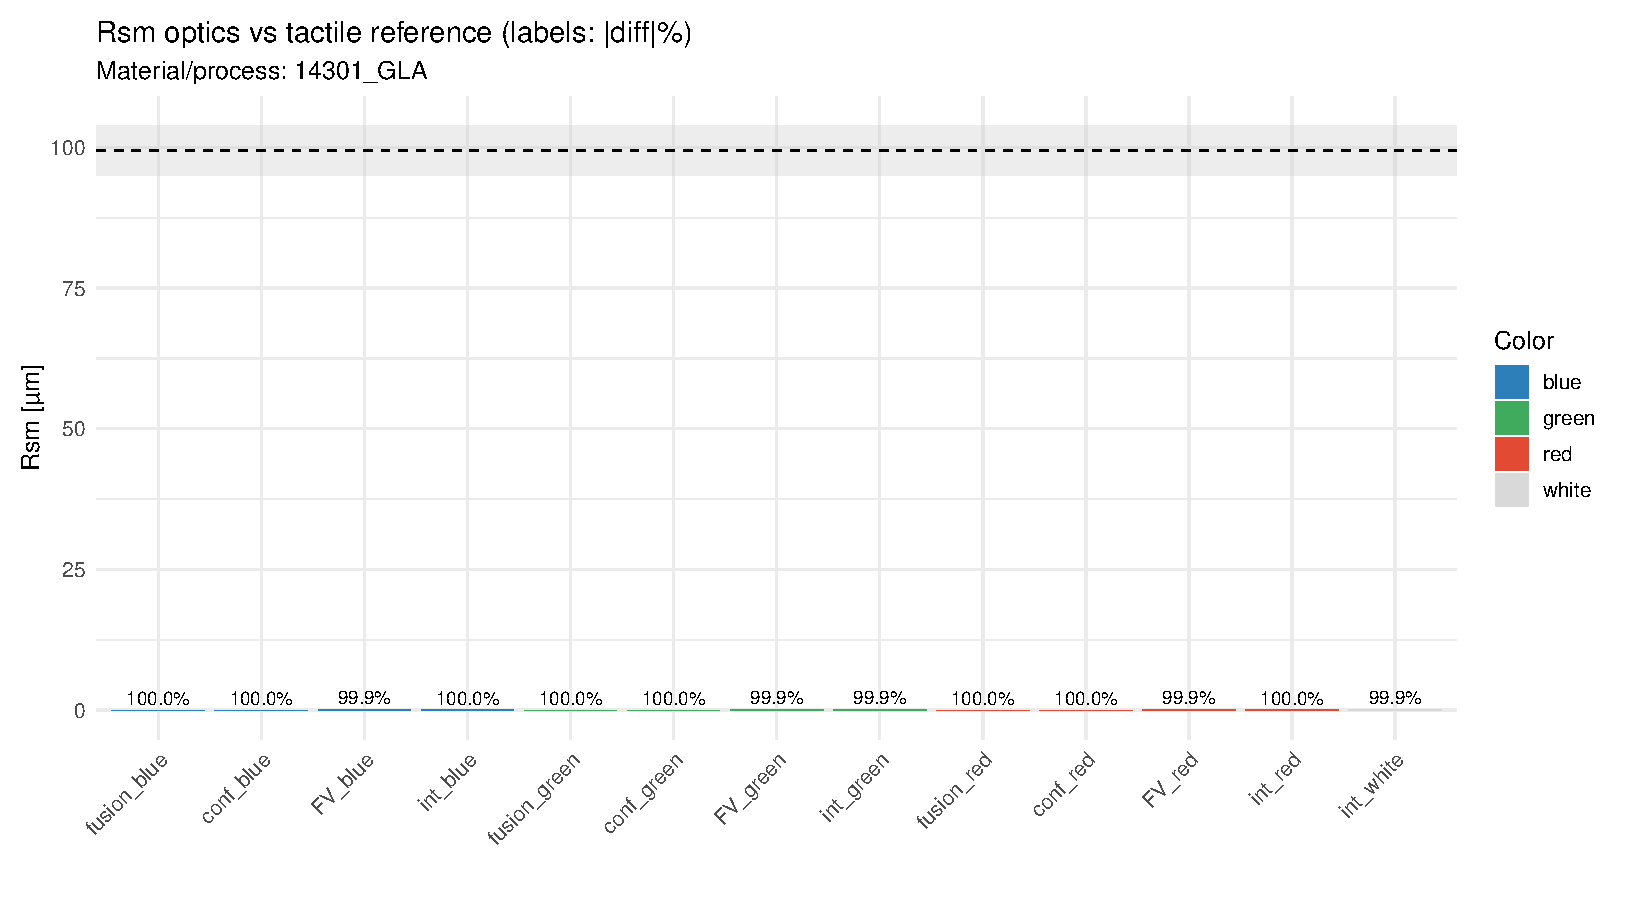
\includegraphics[width=\linewidth]{plots/rsm_abs_14301_gla_optics_vs_tactile.pdf}
\end{minipage}
\begin{minipage}[t]{0.32\textwidth}\centering
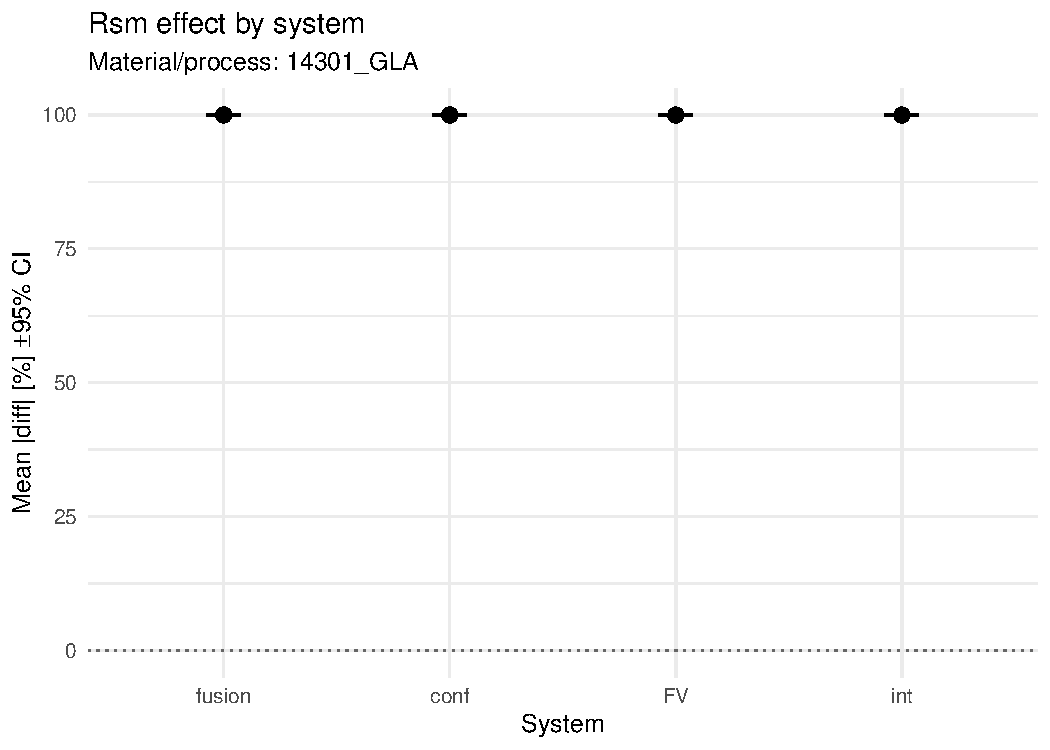
\includegraphics[width=\linewidth]{plots/rsm_abs_14301_gla_effects_by_system.pdf}
\end{minipage}
\begin{minipage}[t]{0.32\textwidth}\centering
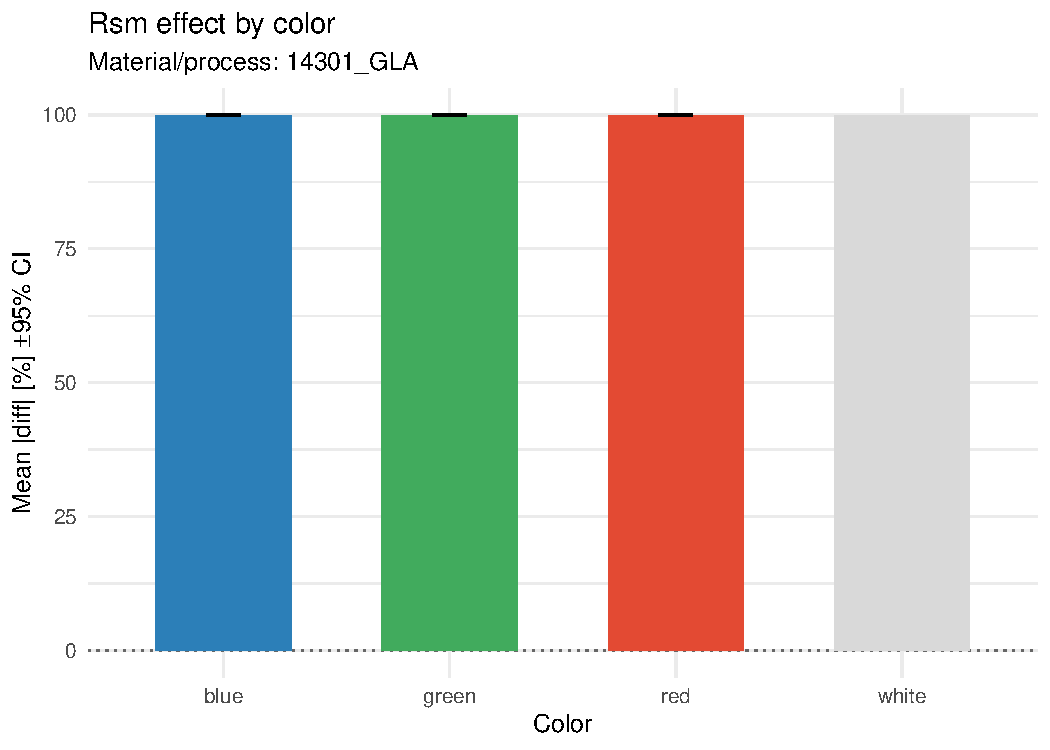
\includegraphics[width=\linewidth]{plots/rsm_abs_14301_gla_effects_by_color.pdf}
\end{minipage}
\caption{RSM — 14301\_gla — porównanie i efekty (|diff| \%)}
\end{figure}

\begin{figure}[H]\centering
\begin{minipage}[t]{0.32\textwidth}\centering
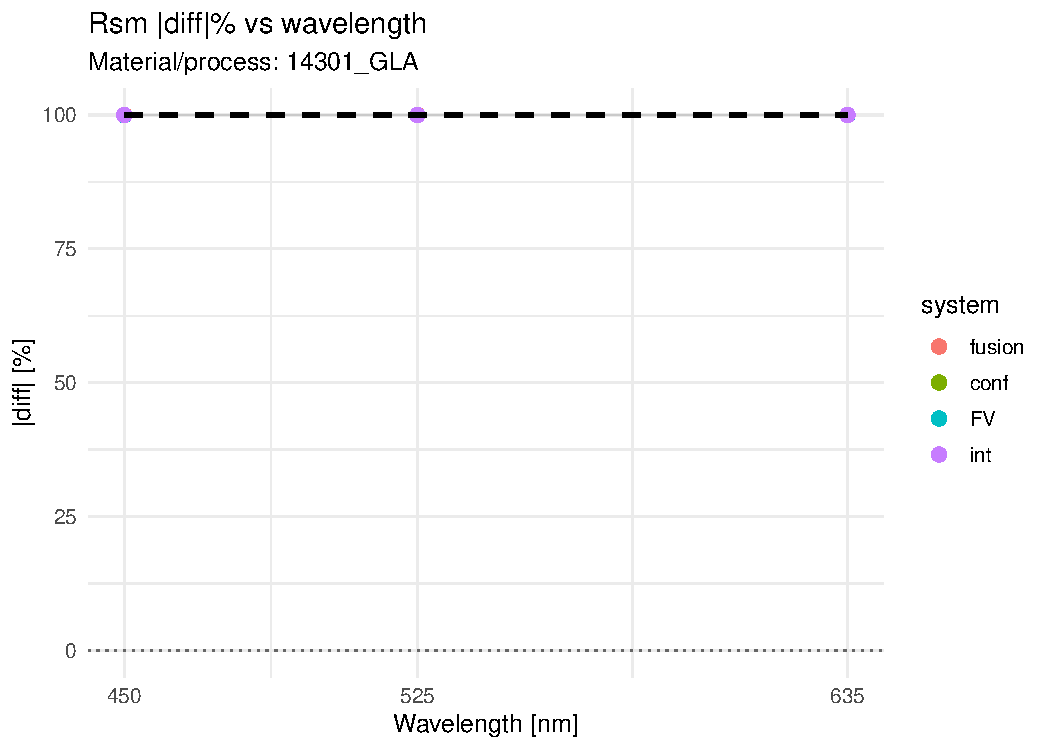
\includegraphics[width=\linewidth]{plots/rsm_abs_14301_gla_diff_vs_wavelength.pdf}
\end{minipage}
\begin{minipage}[t]{0.32\textwidth}\centering
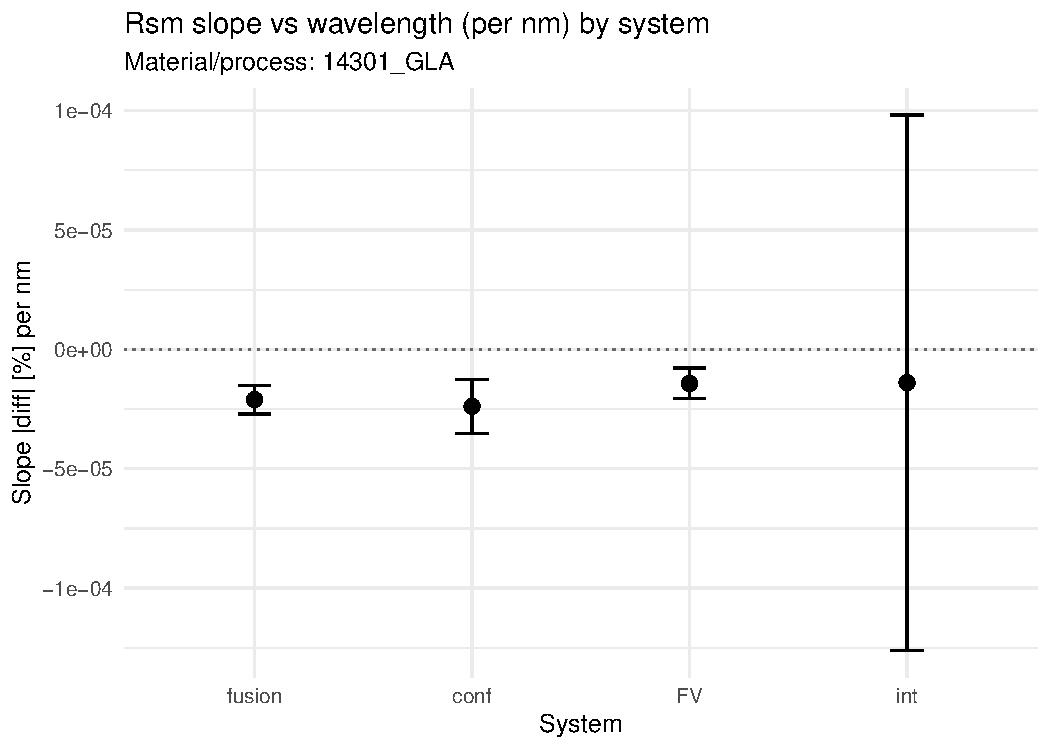
\includegraphics[width=\linewidth]{plots/rsm_abs_14301_gla_slope_by_system_vs_nm.pdf}
\end{minipage}
\begin{minipage}[t]{0.32\textwidth}\centering
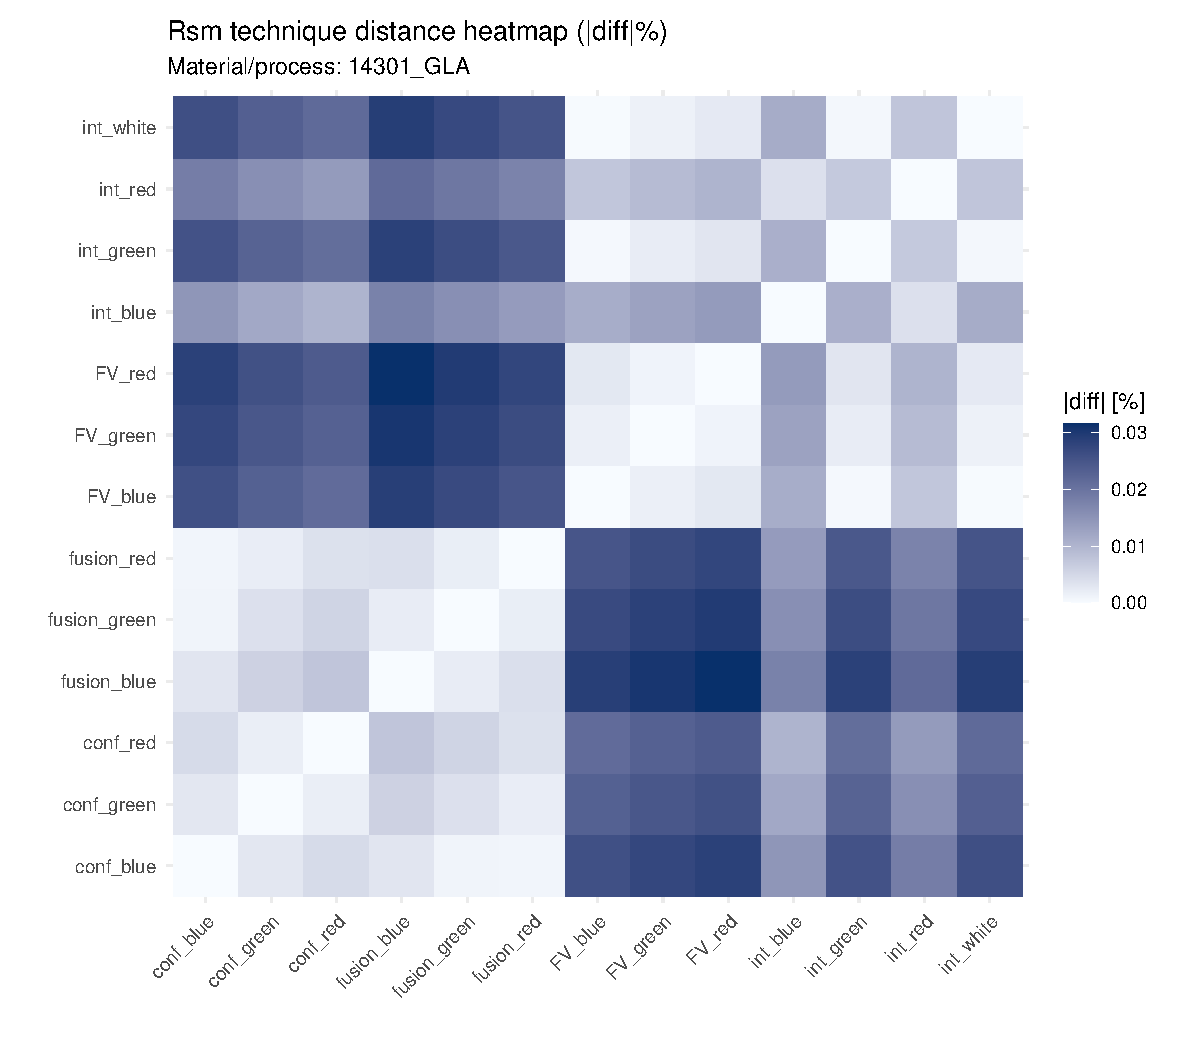
\includegraphics[width=\linewidth]{plots/rsm_abs_14301_gla_tech_distance_heatmap.pdf}
\end{minipage}
\caption{RSM — 14301\_gla — wavelength, nachylenia, odległości technik}
\end{figure}

\begin{figure}[H]\centering
\begin{minipage}[t]{0.32\textwidth}\centering
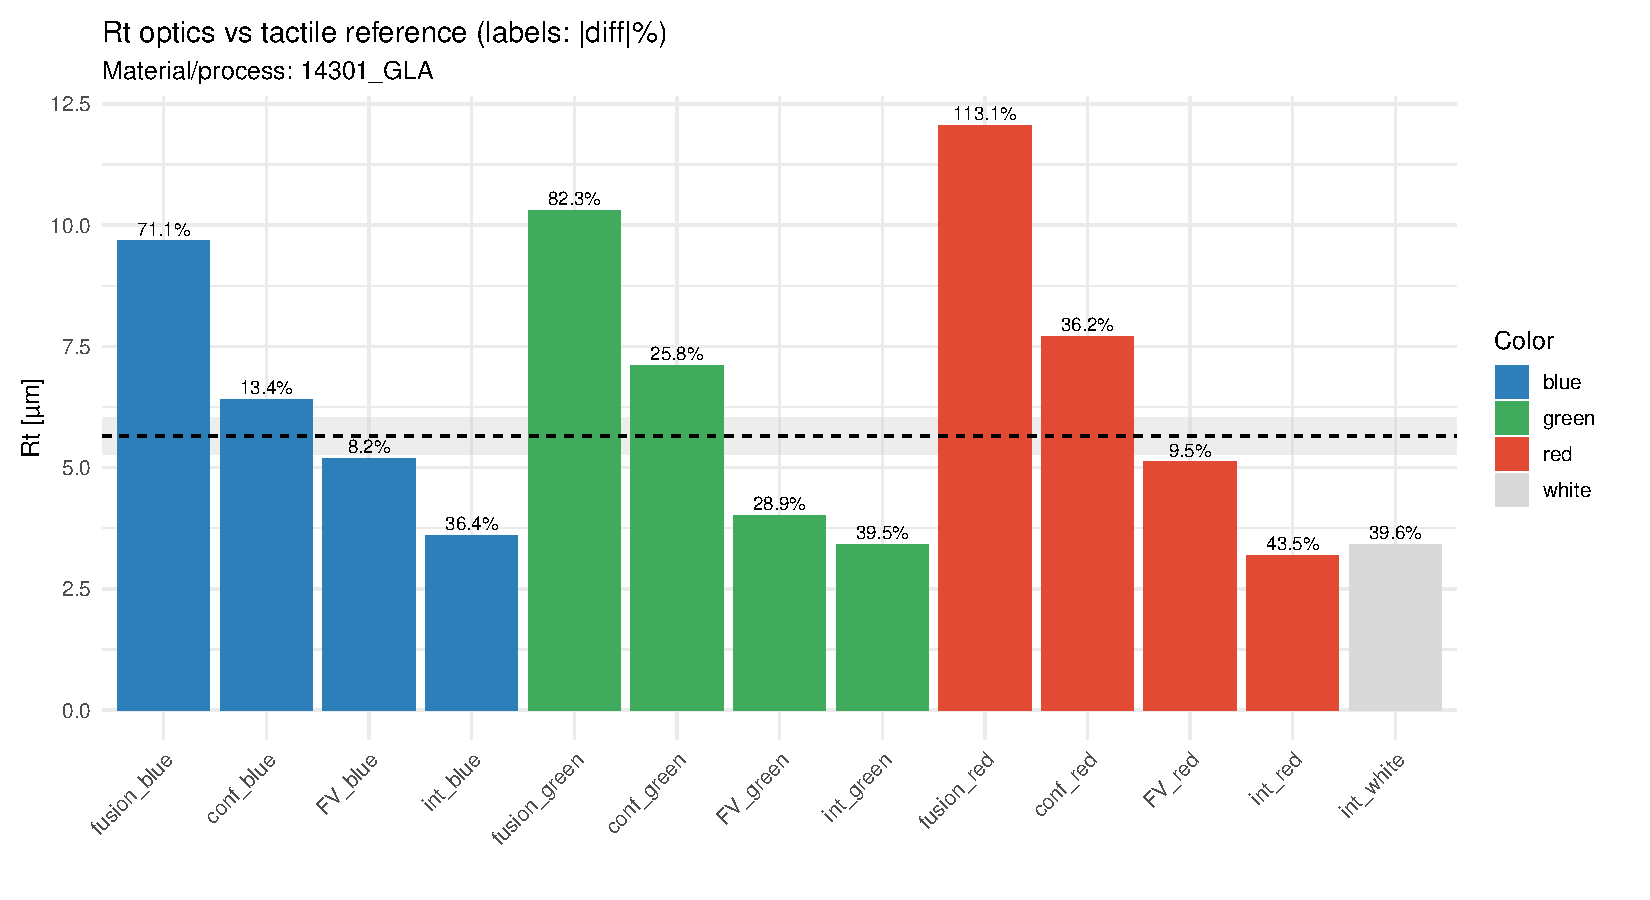
\includegraphics[width=\linewidth]{plots/rt_abs_14301_gla_optics_vs_tactile.pdf}
\end{minipage}
\begin{minipage}[t]{0.32\textwidth}\centering
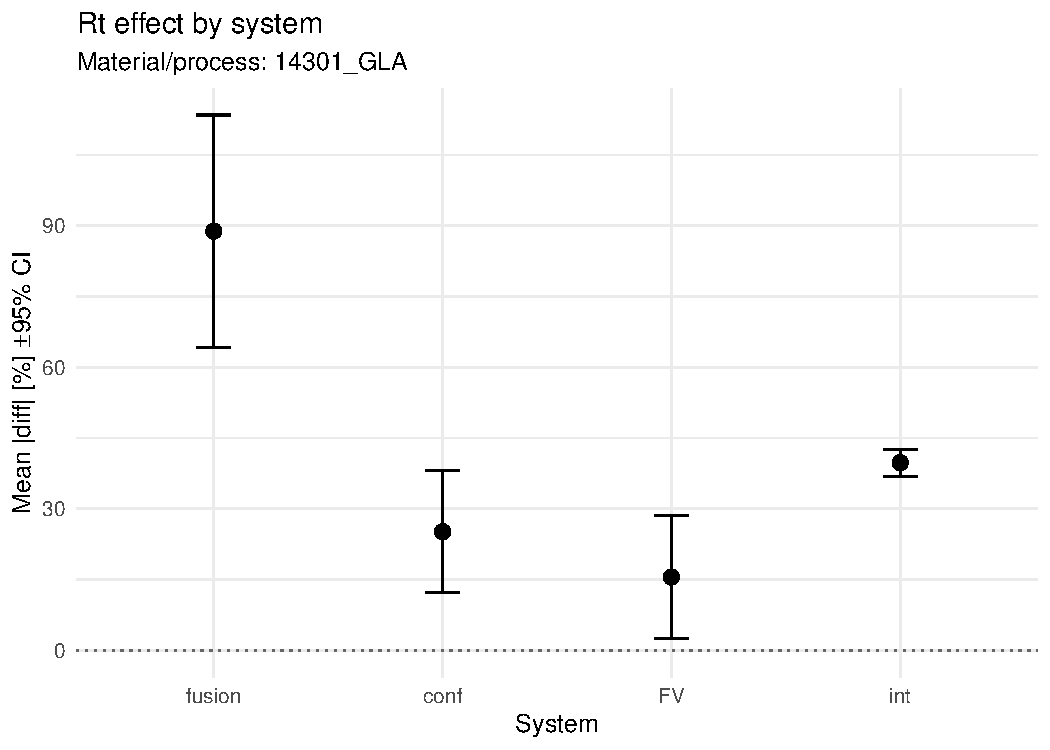
\includegraphics[width=\linewidth]{plots/rt_abs_14301_gla_effects_by_system.pdf}
\end{minipage}
\begin{minipage}[t]{0.32\textwidth}\centering
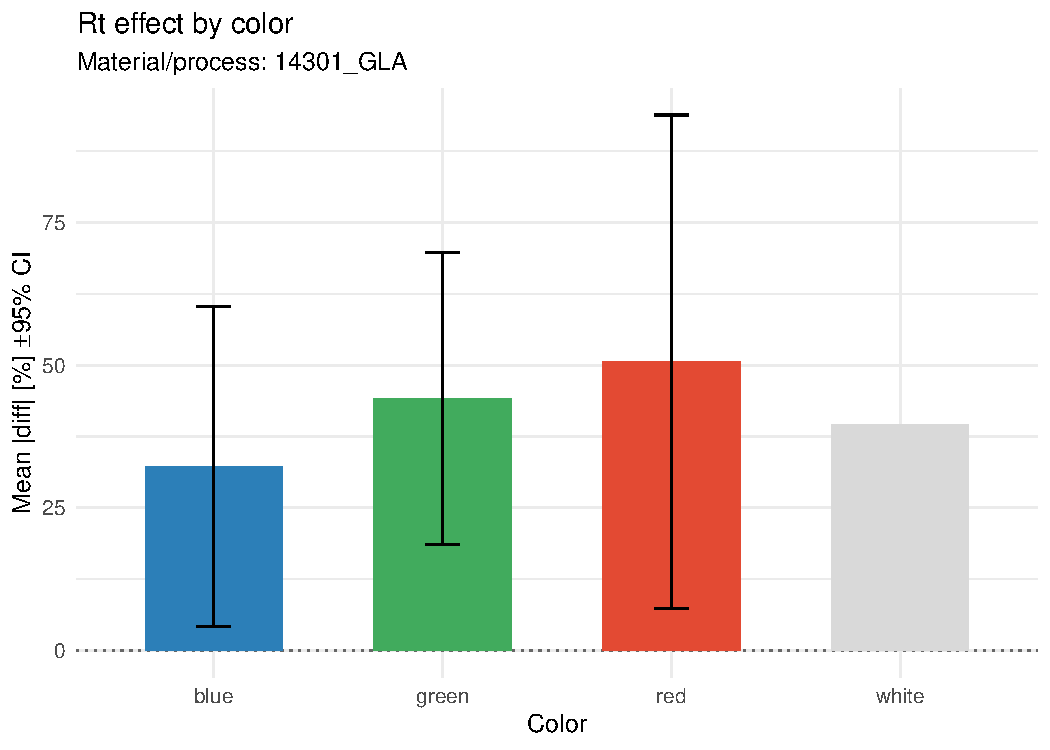
\includegraphics[width=\linewidth]{plots/rt_abs_14301_gla_effects_by_color.pdf}
\end{minipage}
\caption{RT — 14301\_gla — porównanie i efekty (|diff| \%)}
\end{figure}

\begin{figure}[H]\centering
\begin{minipage}[t]{0.32\textwidth}\centering
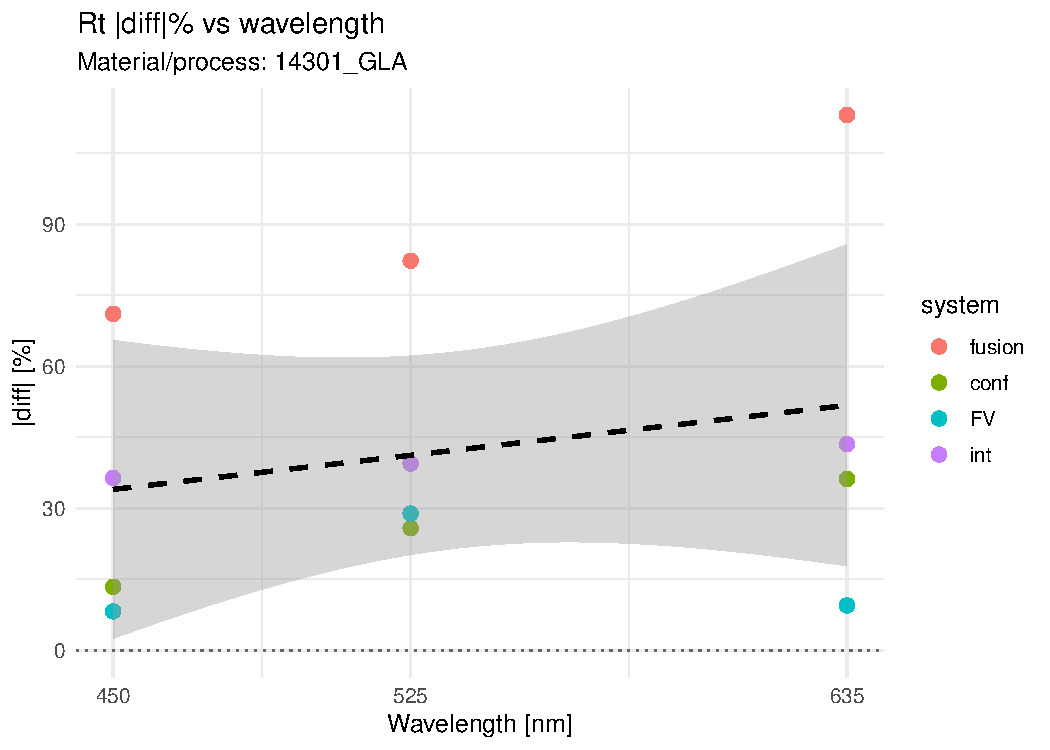
\includegraphics[width=\linewidth]{plots/rt_abs_14301_gla_diff_vs_wavelength.pdf}
\end{minipage}
\begin{minipage}[t]{0.32\textwidth}\centering
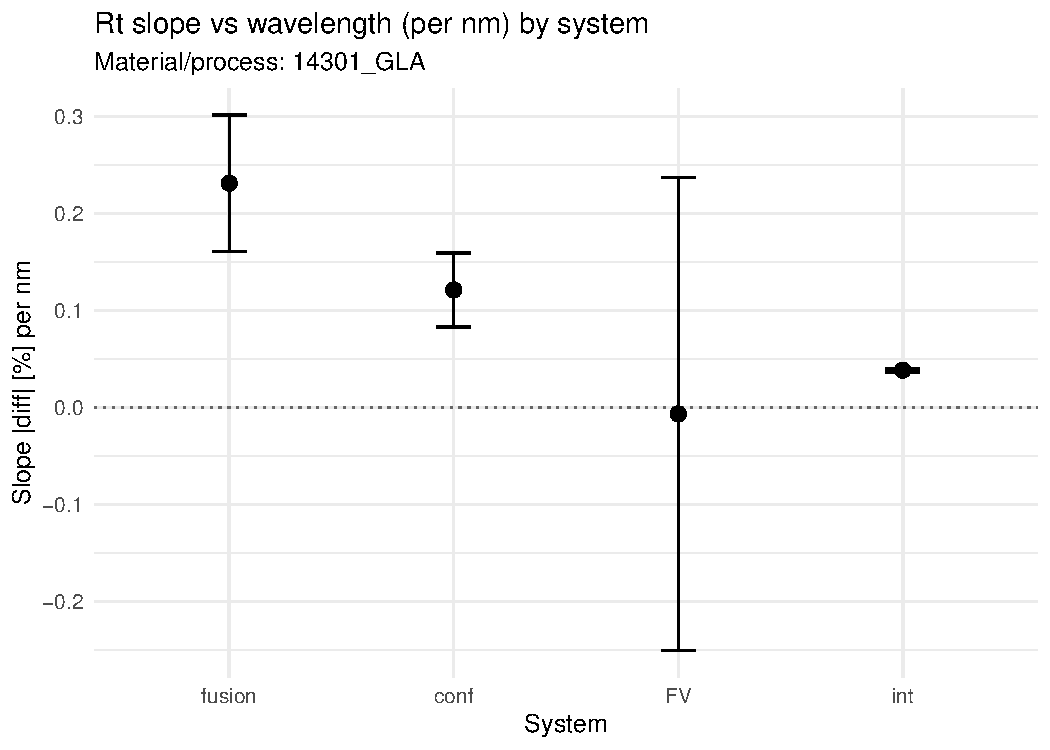
\includegraphics[width=\linewidth]{plots/rt_abs_14301_gla_slope_by_system_vs_nm.pdf}
\end{minipage}
\begin{minipage}[t]{0.32\textwidth}\centering
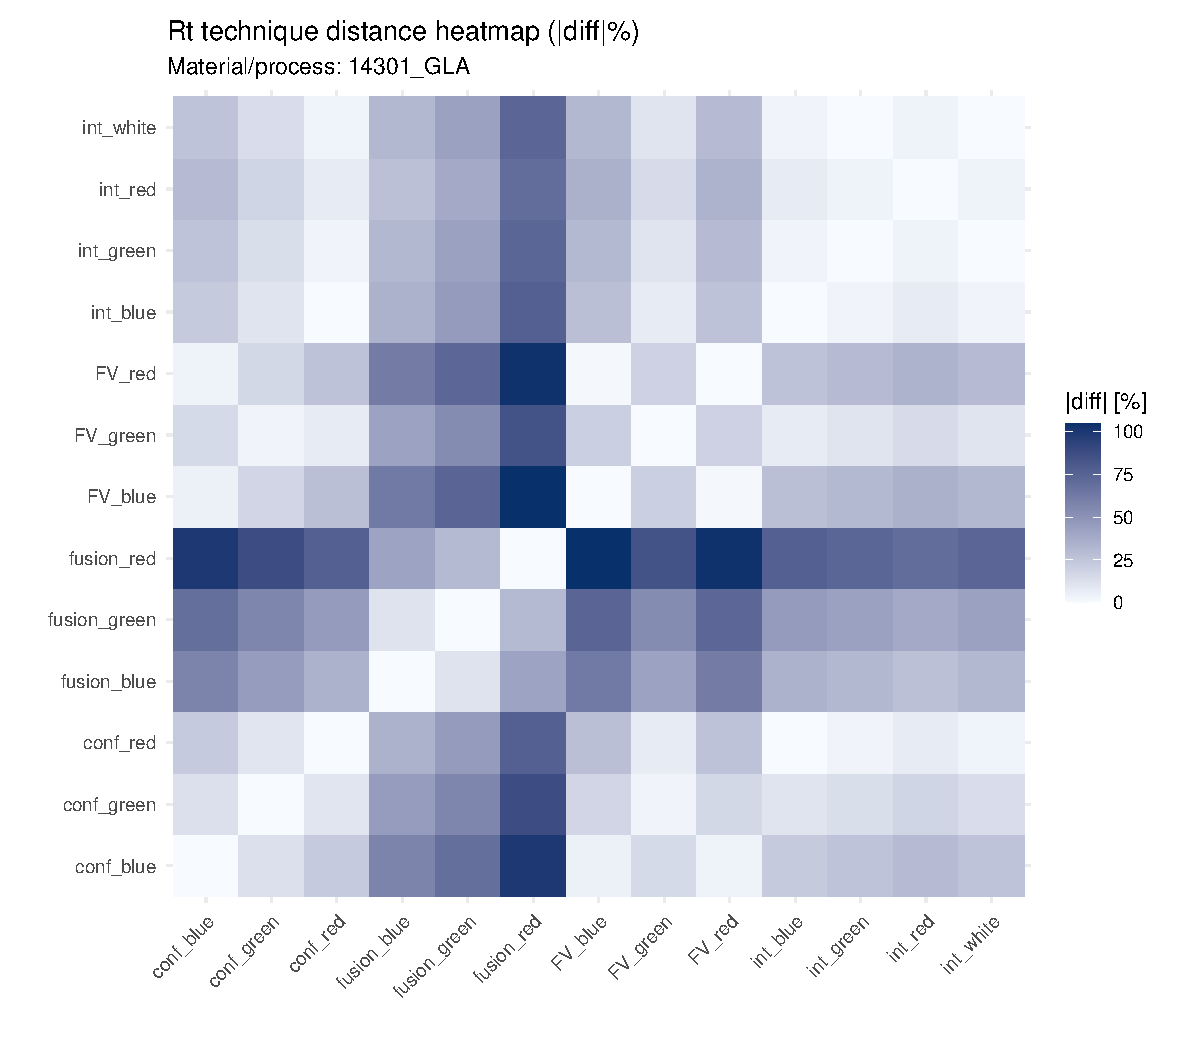
\includegraphics[width=\linewidth]{plots/rt_abs_14301_gla_tech_distance_heatmap.pdf}
\end{minipage}
\caption{RT — 14301\_gla — wavelength, nachylenia, odległości technik}
\end{figure}

\begin{figure}[H]\centering
\begin{minipage}[t]{0.32\textwidth}\centering
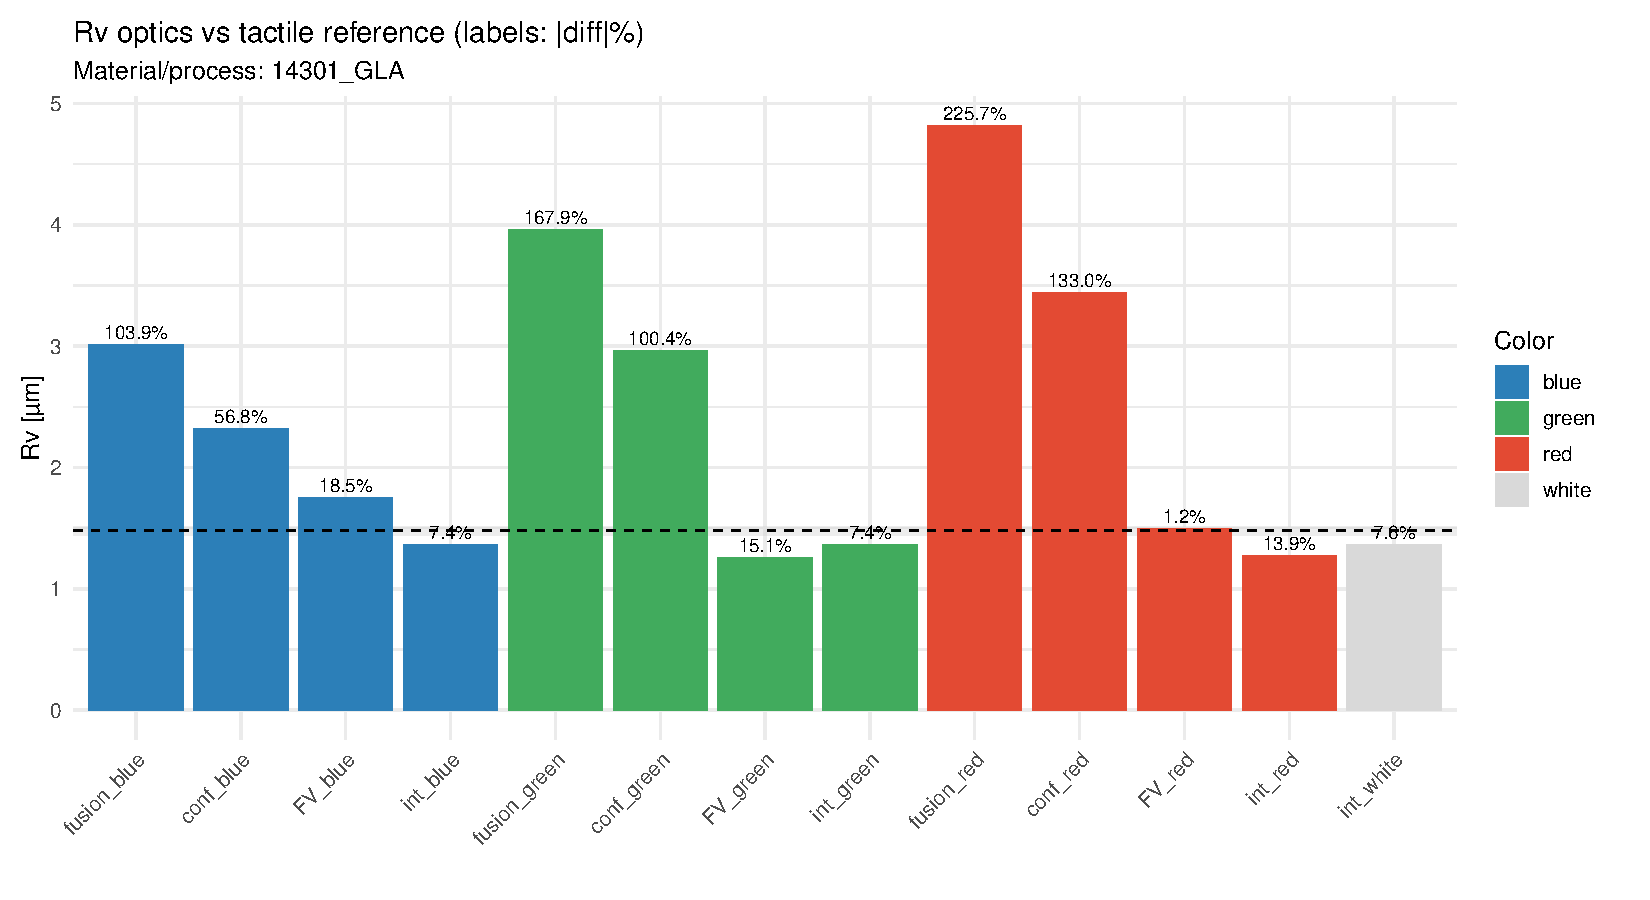
\includegraphics[width=\linewidth]{plots/rv_abs_14301_gla_optics_vs_tactile.pdf}
\end{minipage}
\begin{minipage}[t]{0.32\textwidth}\centering
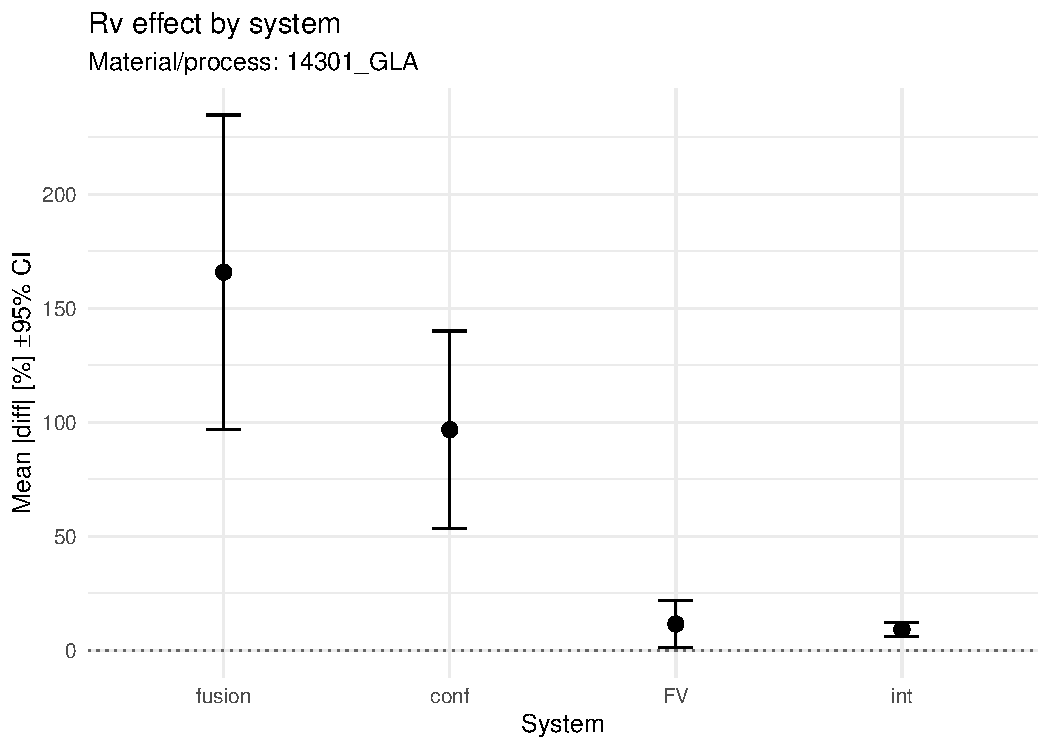
\includegraphics[width=\linewidth]{plots/rv_abs_14301_gla_effects_by_system.pdf}
\end{minipage}
\begin{minipage}[t]{0.32\textwidth}\centering
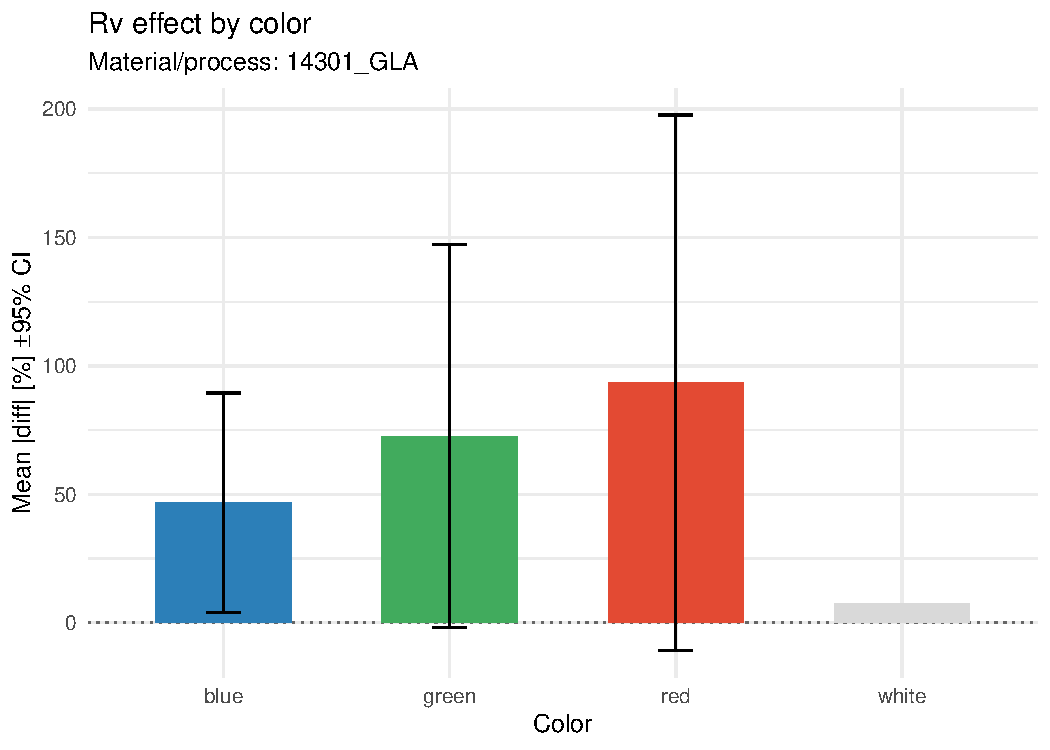
\includegraphics[width=\linewidth]{plots/rv_abs_14301_gla_effects_by_color.pdf}
\end{minipage}
\caption{RV — 14301\_gla — porównanie i efekty (|diff| \%)}
\end{figure}

\begin{figure}[H]\centering
\begin{minipage}[t]{0.32\textwidth}\centering
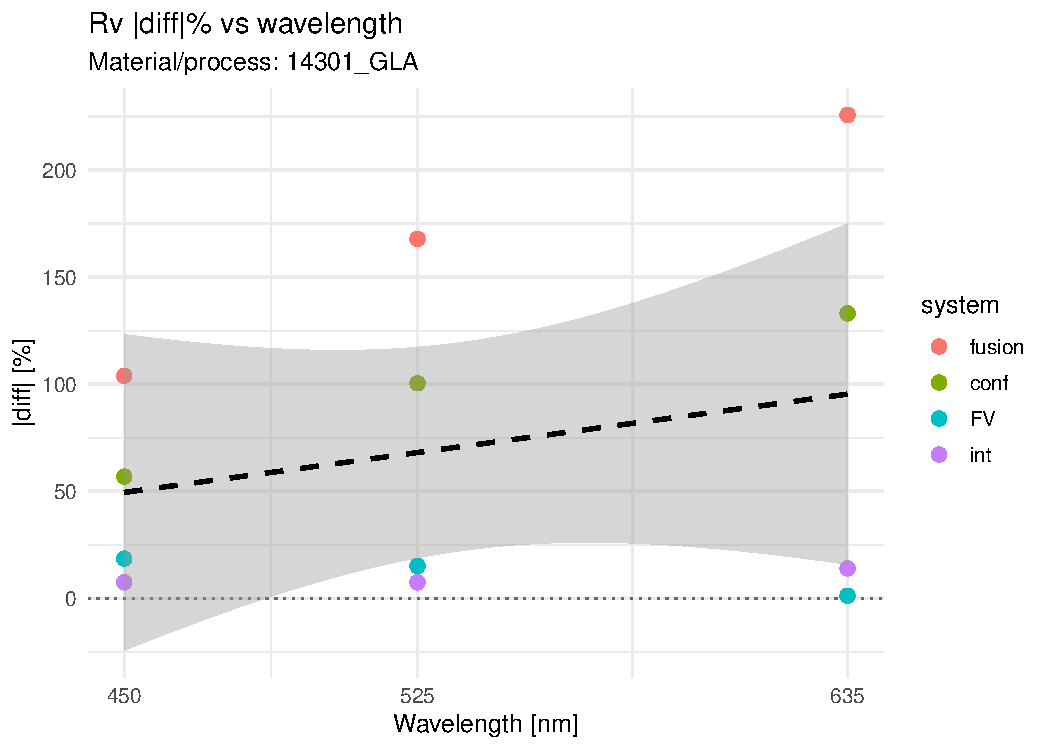
\includegraphics[width=\linewidth]{plots/rv_abs_14301_gla_diff_vs_wavelength.pdf}
\end{minipage}
\begin{minipage}[t]{0.32\textwidth}\centering
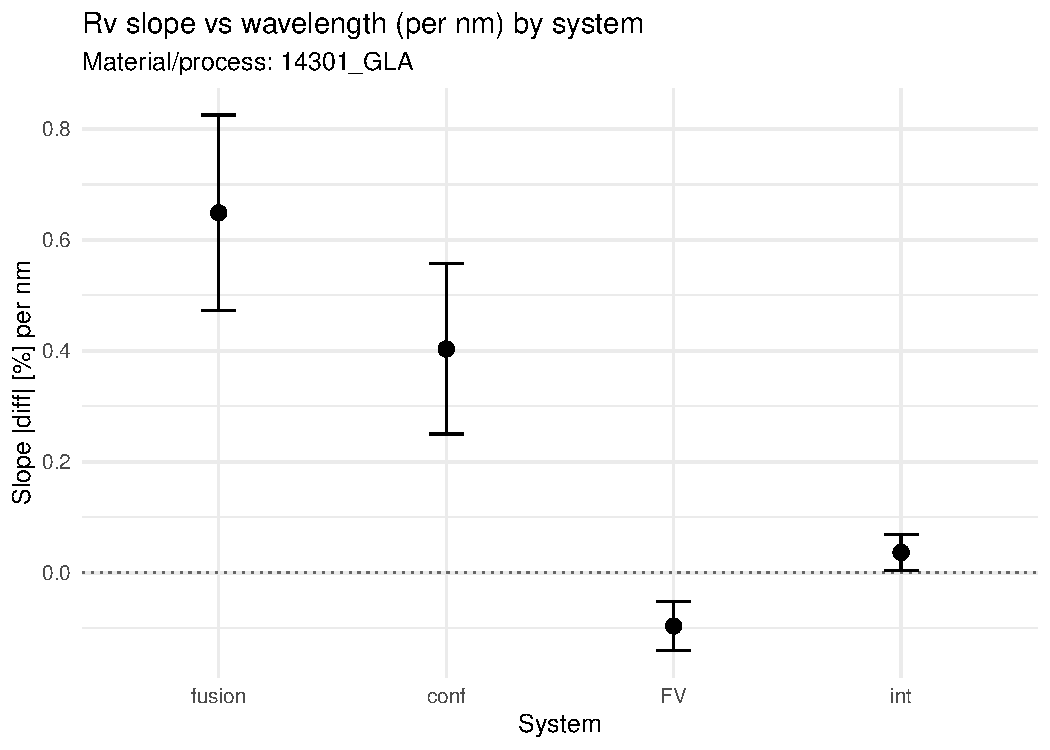
\includegraphics[width=\linewidth]{plots/rv_abs_14301_gla_slope_by_system_vs_nm.pdf}
\end{minipage}
\begin{minipage}[t]{0.32\textwidth}\centering
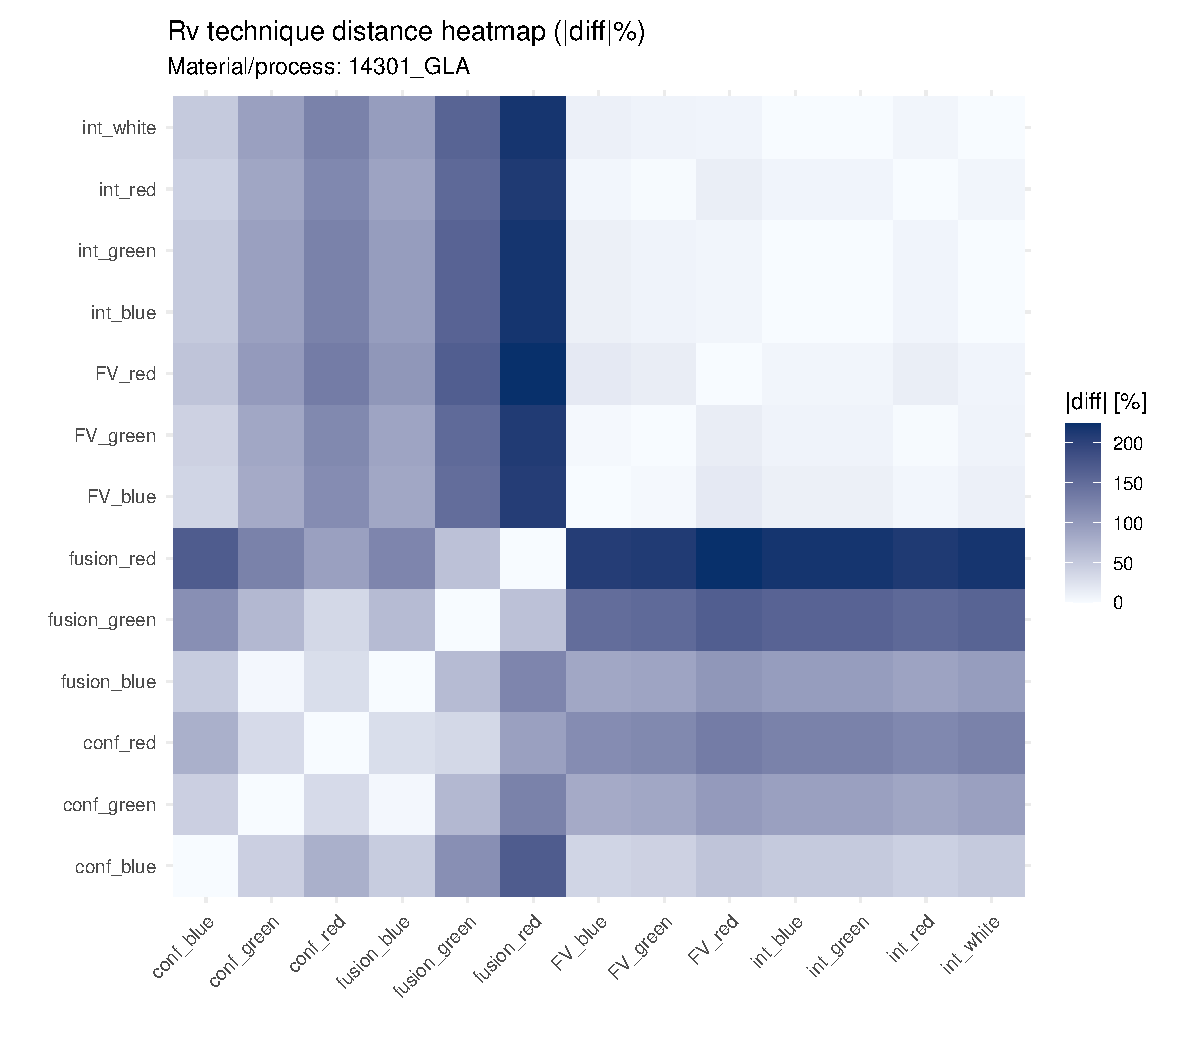
\includegraphics[width=\linewidth]{plots/rv_abs_14301_gla_tech_distance_heatmap.pdf}
\end{minipage}
\caption{RV — 14301\_gla — wavelength, nachylenia, odległości technik}
\end{figure}

\begin{figure}[H]\centering
\begin{minipage}[t]{0.32\textwidth}\centering
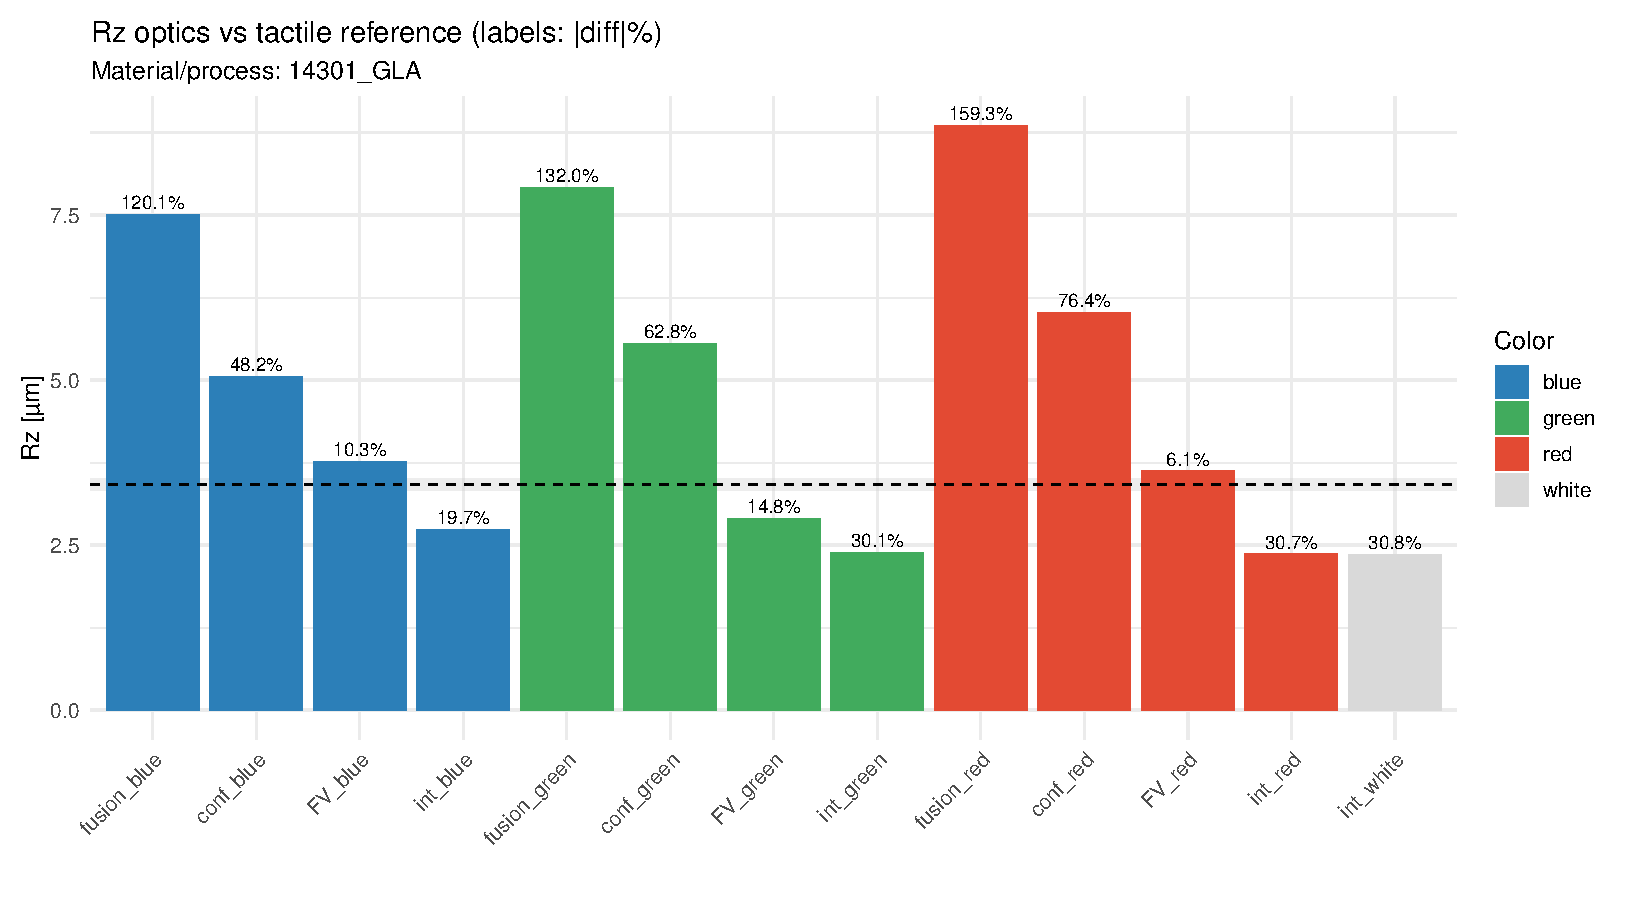
\includegraphics[width=\linewidth]{plots/rz_abs_14301_gla_optics_vs_tactile.pdf}
\end{minipage}
\begin{minipage}[t]{0.32\textwidth}\centering
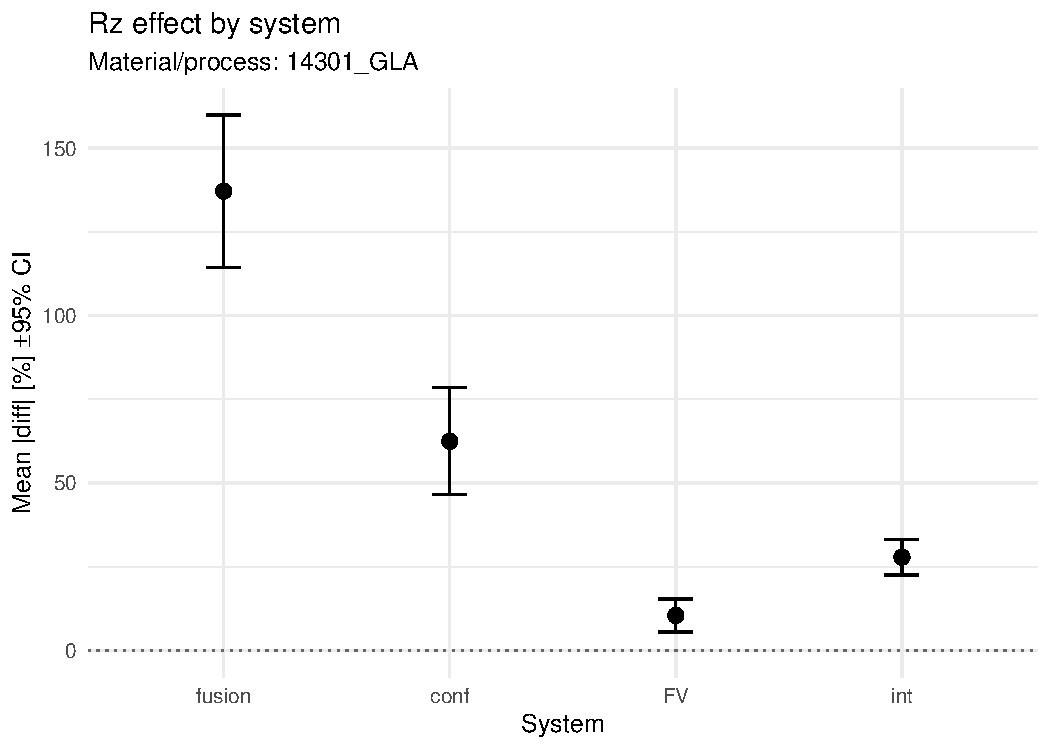
\includegraphics[width=\linewidth]{plots/rz_abs_14301_gla_effects_by_system.pdf}
\end{minipage}
\begin{minipage}[t]{0.32\textwidth}\centering
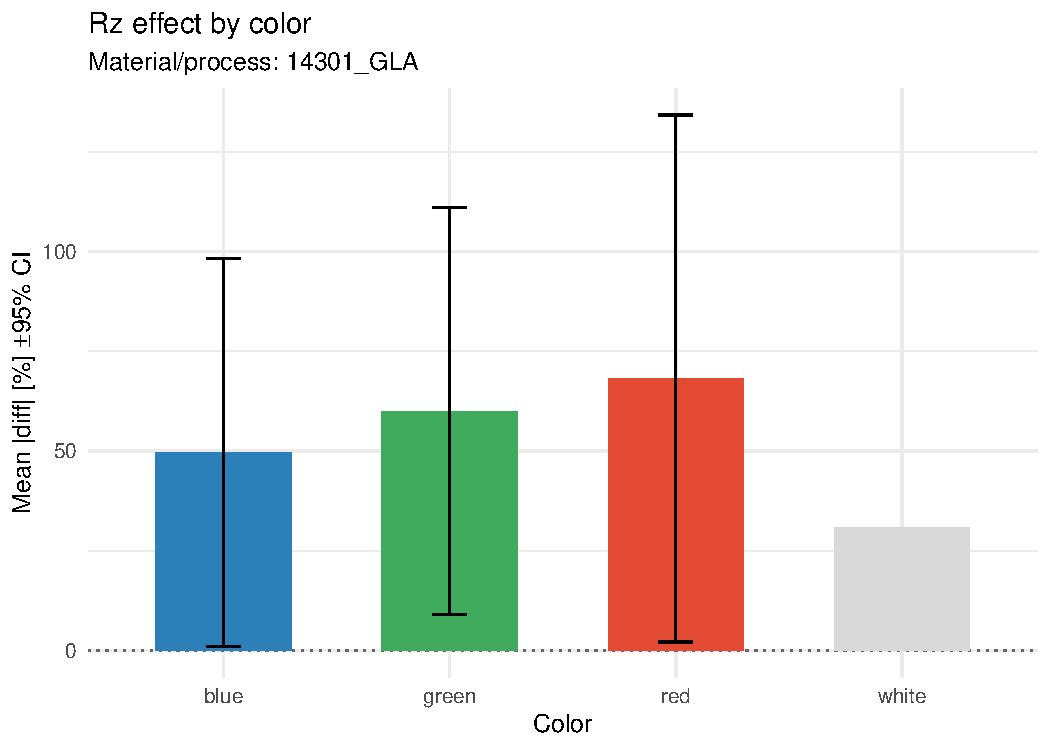
\includegraphics[width=\linewidth]{plots/rz_abs_14301_gla_effects_by_color.pdf}
\end{minipage}
\caption{RZ — 14301\_gla — porównanie i efekty (|diff| \%)}
\end{figure}

\begin{figure}[H]\centering
\begin{minipage}[t]{0.32\textwidth}\centering
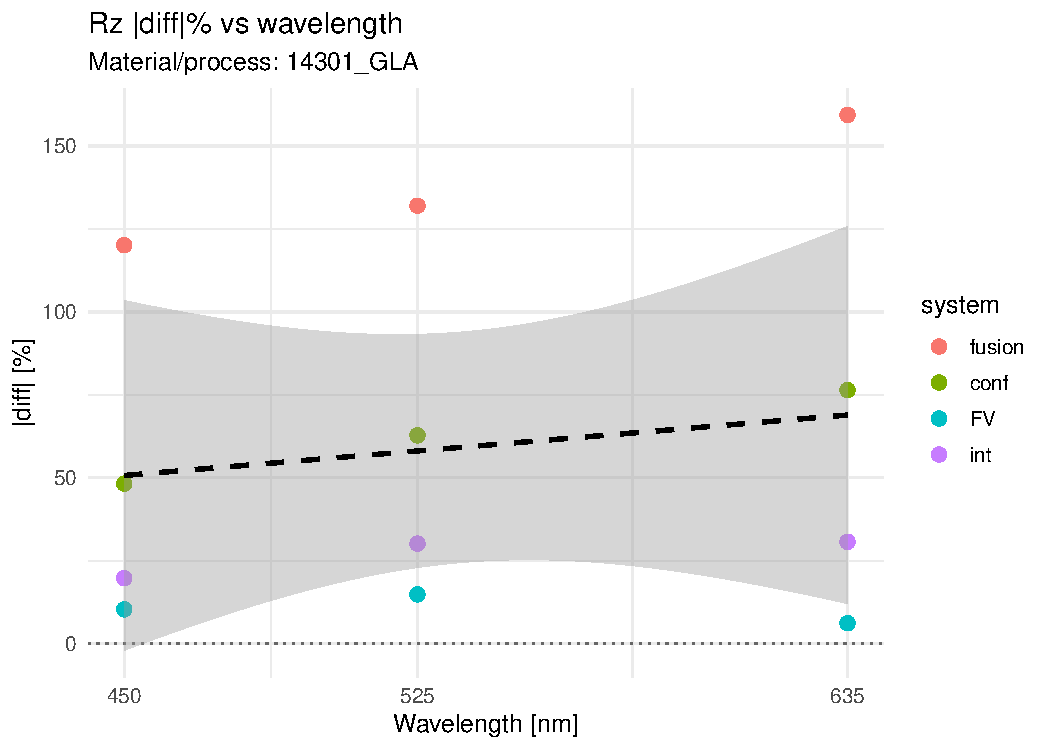
\includegraphics[width=\linewidth]{plots/rz_abs_14301_gla_diff_vs_wavelength.pdf}
\end{minipage}
\begin{minipage}[t]{0.32\textwidth}\centering
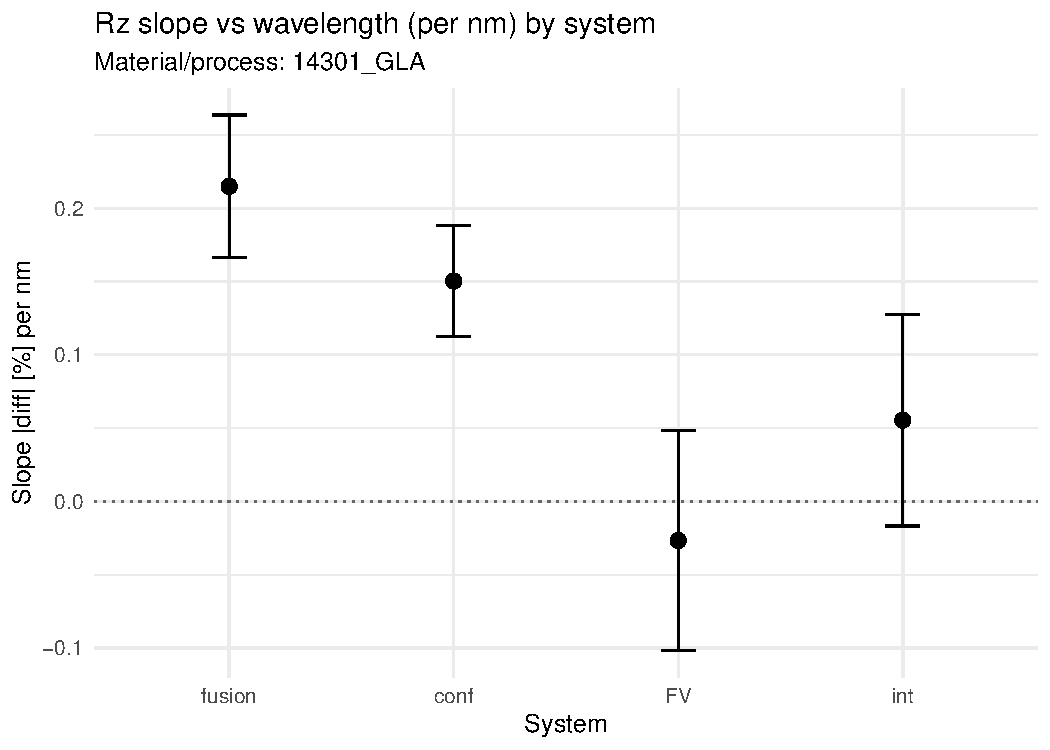
\includegraphics[width=\linewidth]{plots/rz_abs_14301_gla_slope_by_system_vs_nm.pdf}
\end{minipage}
\begin{minipage}[t]{0.32\textwidth}\centering
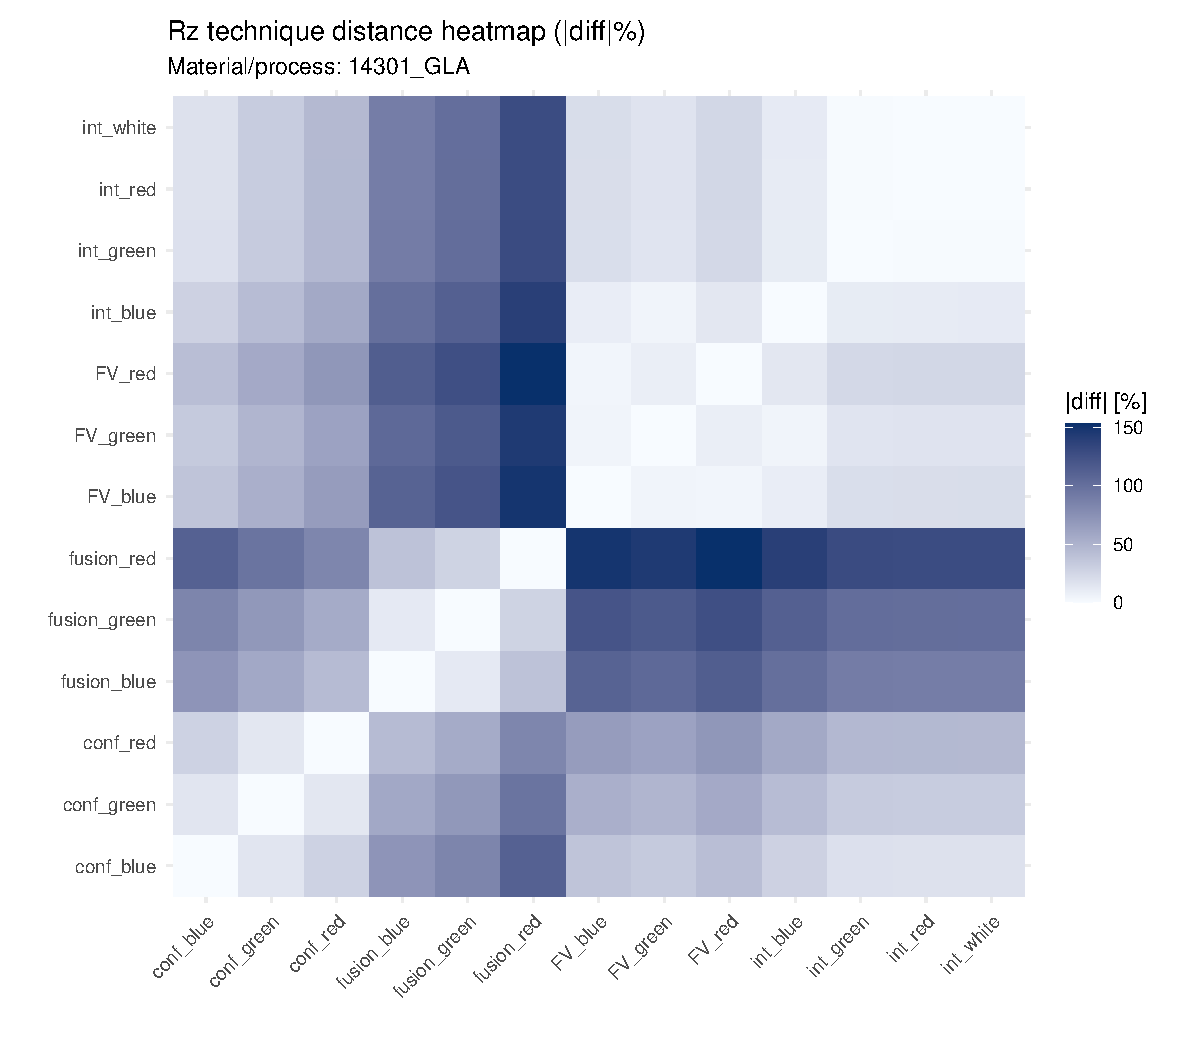
\includegraphics[width=\linewidth]{plots/rz_abs_14301_gla_tech_distance_heatmap.pdf}
\end{minipage}
\caption{RZ — 14301\_gla — wavelength, nachylenia, odległości technik}
\end{figure}

\begin{figure}[H]\centering
\begin{minipage}[t]{0.32\textwidth}\centering
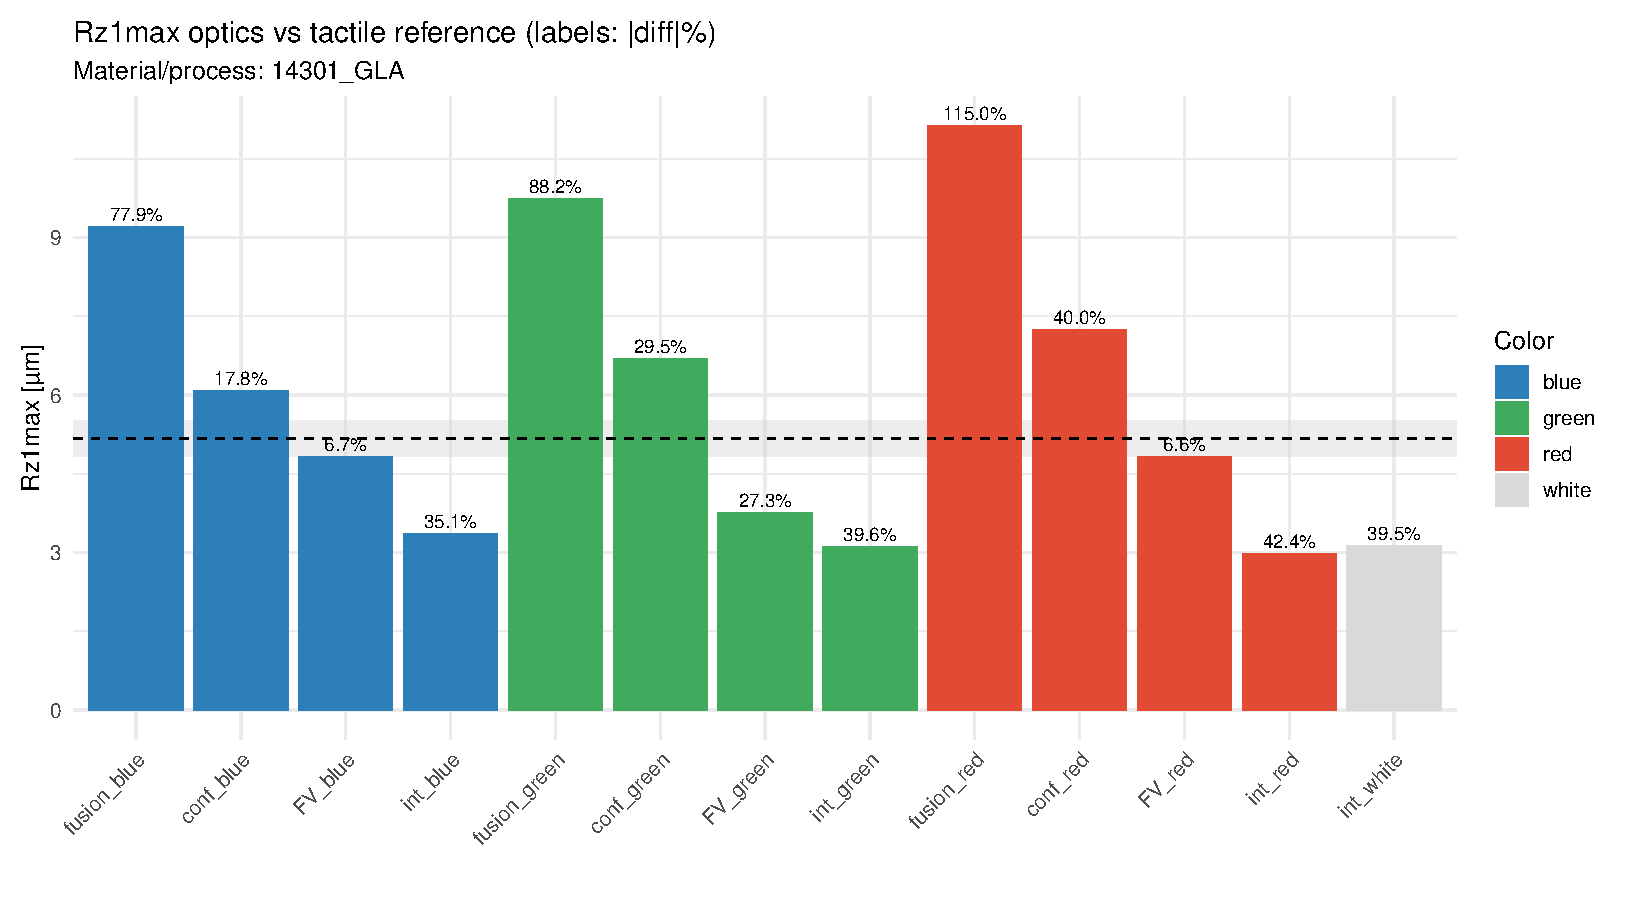
\includegraphics[width=\linewidth]{plots/rz1max_abs_14301_gla_optics_vs_tactile.pdf}
\end{minipage}
\begin{minipage}[t]{0.32\textwidth}\centering
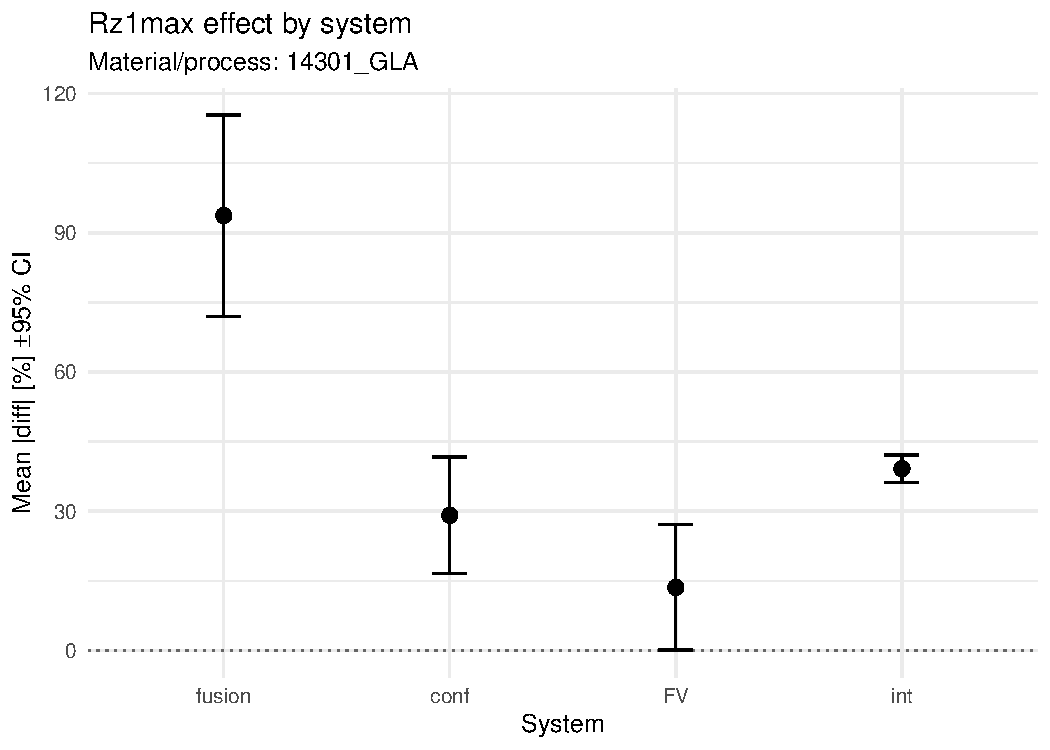
\includegraphics[width=\linewidth]{plots/rz1max_abs_14301_gla_effects_by_system.pdf}
\end{minipage}
\begin{minipage}[t]{0.32\textwidth}\centering
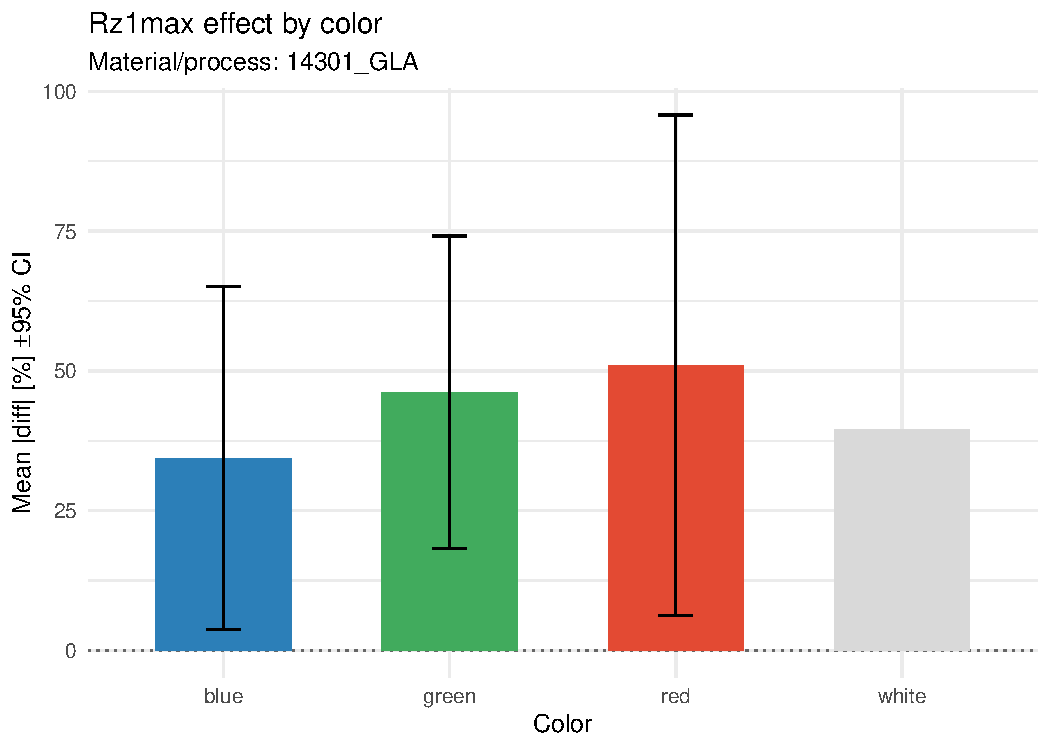
\includegraphics[width=\linewidth]{plots/rz1max_abs_14301_gla_effects_by_color.pdf}
\end{minipage}
\caption{RZ1MAX — 14301\_gla — porównanie i efekty (|diff| \%)}
\end{figure}

\begin{figure}[H]\centering
\begin{minipage}[t]{0.32\textwidth}\centering
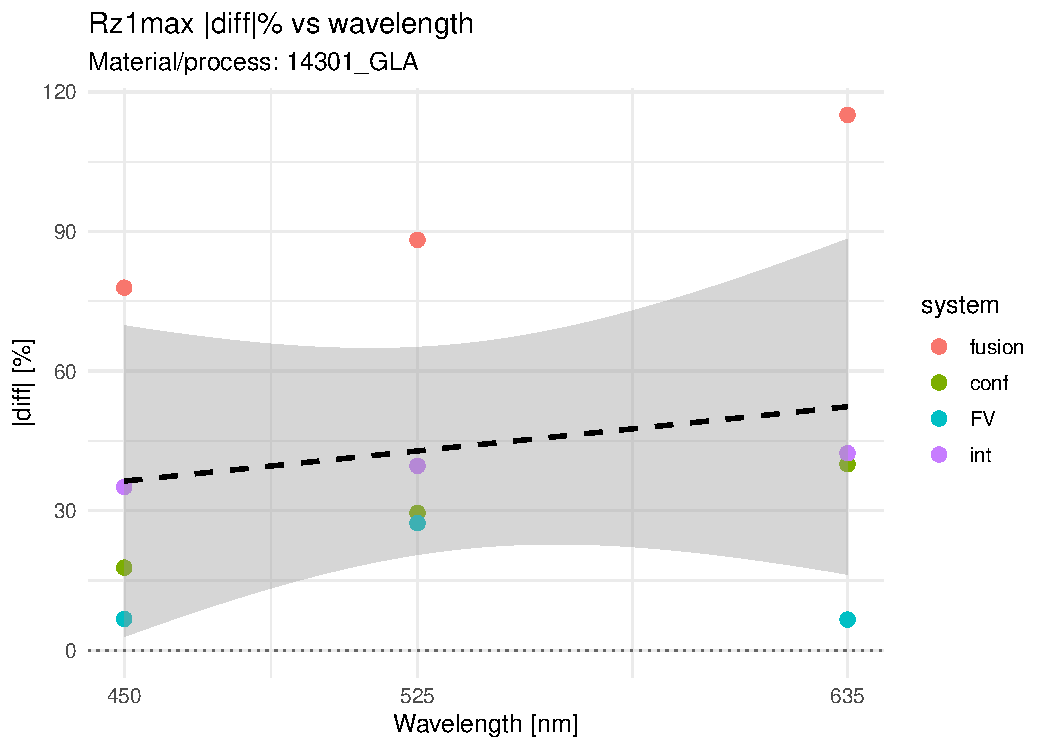
\includegraphics[width=\linewidth]{plots/rz1max_abs_14301_gla_diff_vs_wavelength.pdf}
\end{minipage}
\begin{minipage}[t]{0.32\textwidth}\centering
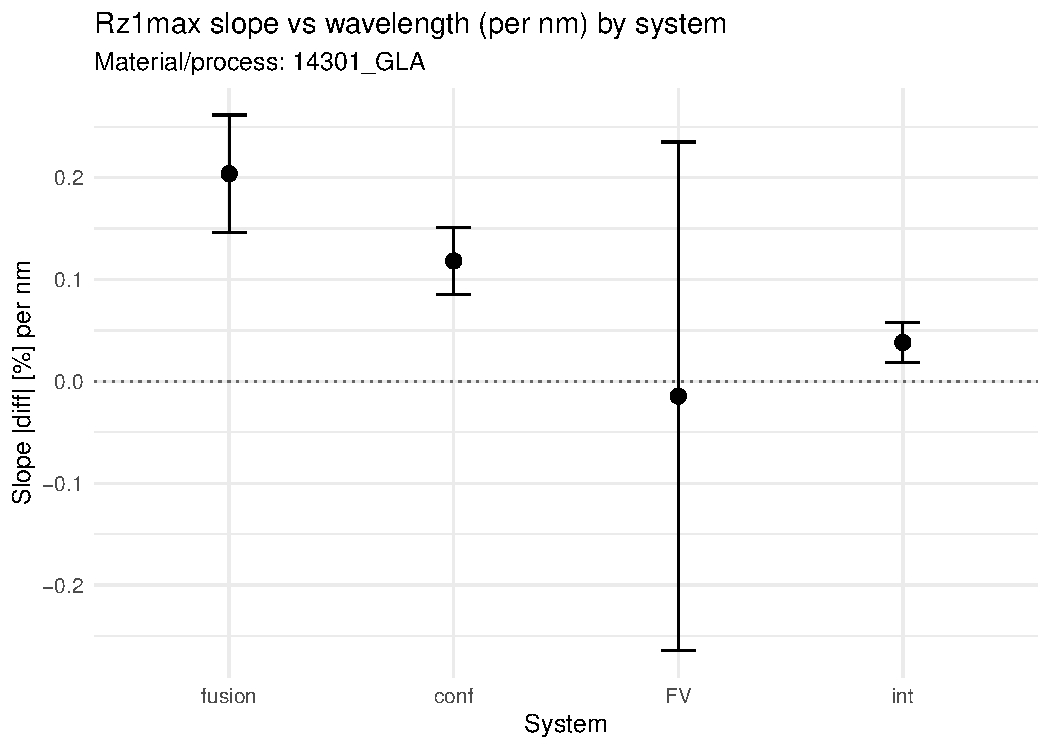
\includegraphics[width=\linewidth]{plots/rz1max_abs_14301_gla_slope_by_system_vs_nm.pdf}
\end{minipage}
\begin{minipage}[t]{0.32\textwidth}\centering
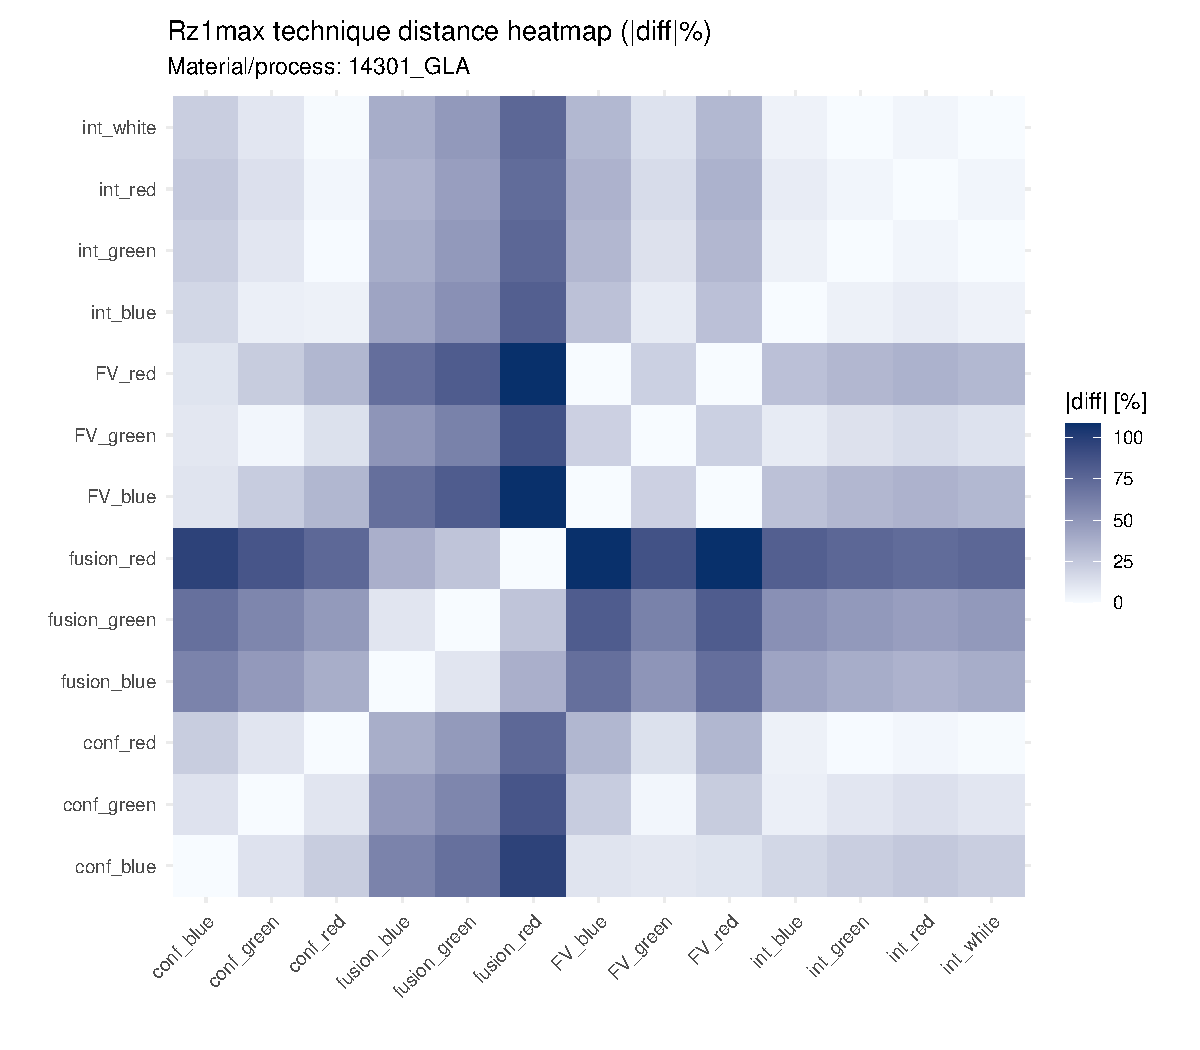
\includegraphics[width=\linewidth]{plots/rz1max_abs_14301_gla_tech_distance_heatmap.pdf}
\end{minipage}
\caption{RZ1MAX — 14301\_gla — wavelength, nachylenia, odległości technik}
\end{figure}

\subsection{Wyniki i wnioski dla materiał/proces: 14301\_gla}

\textbf{RA}. r=0.242, rho=0.207; eta2: system=0.828, color=0.080.
Istotne nachylenia: fusion(slope=0.161, p=0.013). Trendy
(p\textless0.1): conf(slope=0.188, p=0.085). Wniosek: TAK. \textbf{RKU}.
r=-0.379, rho=-0.355; eta2: system=0.494, color=0.168. Istotne
nachylenia: int(slope=-0.065, p=0.016). Wniosek: TAK. \textbf{RP}.
r=-0.030, rho=0.059; eta2: system=0.959, color=0.004. Wniosek: NIE.
\textbf{RQ}. r=0.191, rho=0.207; eta2: system=0.886, color=0.048. Trendy
(p\textless0.1): conf(slope=0.180, p=0.078). Wniosek: NIE. \textbf{RSK}.
r=0.364, rho=0.384; eta2: system=0.545, color=0.164. Wniosek: NIE.
\textbf{RSM}. r=-0.115, rho=-0.266; eta2: system=0.941, color=0.039.
Trendy (p\textless0.1): fusion(slope=-0.000, p=0.091). Wniosek: NIE.
\textbf{RT}. r=0.240, rho=0.236; eta2: system=0.864, color=0.062.
Istotne nachylenia: int(slope=0.038, p=0.016). Trendy (p\textless0.1):
fusion(slope=0.231, p=0.098). Wniosek: TAK. \textbf{RV}. r=0.264,
rho=0.059; eta2: system=0.838, color=0.068. Trendy (p\textless0.1):
fusion(slope=0.649, p=0.088). Wniosek: NIE. \textbf{RZ}. r=0.150,
rho=0.148; eta2: system=0.956, color=0.023. Trendy (p\textless0.1):
conf(slope=0.150, p=0.081); fusion(slope=0.215, p=0.073). Wniosek: NIE.
\textbf{RZ1MAX}. r=0.206, rho=0.266; eta2: system=0.894, color=0.048.
Trendy (p\textless0.1): conf(slope=0.118, p=0.090); fusion(slope=0.204,
p=0.091). Wniosek: NIE.

\paragraph{Podsumowanie (opisowe) dla tego materiału/procesu}
\begin{itemize}
\item W ujęciu ANOVA: częściej dominuje system (eta²).
\item Najczęściej preferowany system (min średni |diff|): FV.
\item Najczęściej preferowana barwa (min średni |diff|): blue.
\item Zależność od wavelength wykryta (p<0.05) dla parametrów: RA, RKU, RT; dotyczy systemów: fusion, int.
\end{itemize}
\paragraph{Rekomendacje dla tego materiału}
\begin{itemize}
\item RA: preferowany system (min średni |diff|): FV; preferowana barwa (min średni |diff|): blue; dominuje system; zależność od wavelength: TAK (p<0.05) — fusion: rośnie.
\item RKU: preferowany system (min średni |diff|): conf; preferowana barwa (min średni |diff|): red; dominuje system; zależność od wavelength: TAK (p<0.05) — int: maleje.
\item RP: preferowany system (min średni |diff|): FV; preferowana barwa (min średni |diff|): white; dominuje system; zależność od wavelength: NIE (brak wykrytego trendu per system).
\item RQ: preferowany system (min średni |diff|): FV; preferowana barwa (min średni |diff|): blue; dominuje system; zależność od wavelength: trend (p<0.1) — conf: rośnie.
\item RSK: preferowany system (min średni |diff|): FV; preferowana barwa (min średni |diff|): blue; dominuje system; zależność od wavelength: NIE (brak wykrytego trendu per system).
\item RSM: preferowany system (min średni |diff|): FV; preferowana barwa (min średni |diff|): white; dominuje system; zależność od wavelength: trend (p<0.1) — fusion: maleje.
\item RT: preferowany system (min średni |diff|): FV; preferowana barwa (min średni |diff|): blue; dominuje system; zależność od wavelength: TAK (p<0.05) — int: rośnie.
\item RV: preferowany system (min średni |diff|): int; preferowana barwa (min średni |diff|): white; dominuje system; zależność od wavelength: trend (p<0.1) — fusion: rośnie.
\item RZ: preferowany system (min średni |diff|): FV; preferowana barwa (min średni |diff|): white; dominuje system; zależność od wavelength: trend (p<0.1) — conf: rośnie; fusion: rośnie.
\item RZ1MAX: preferowany system (min średni |diff|): FV; preferowana barwa (min średni |diff|): blue; dominuje system; zależność od wavelength: trend (p<0.1) — conf: rośnie; fusion: rośnie.
\end{itemize}
\subsubsection{Materiał/proces: 14301\_gri}
\begin{figure}[H]\centering
\begin{minipage}[t]{0.32\textwidth}\centering
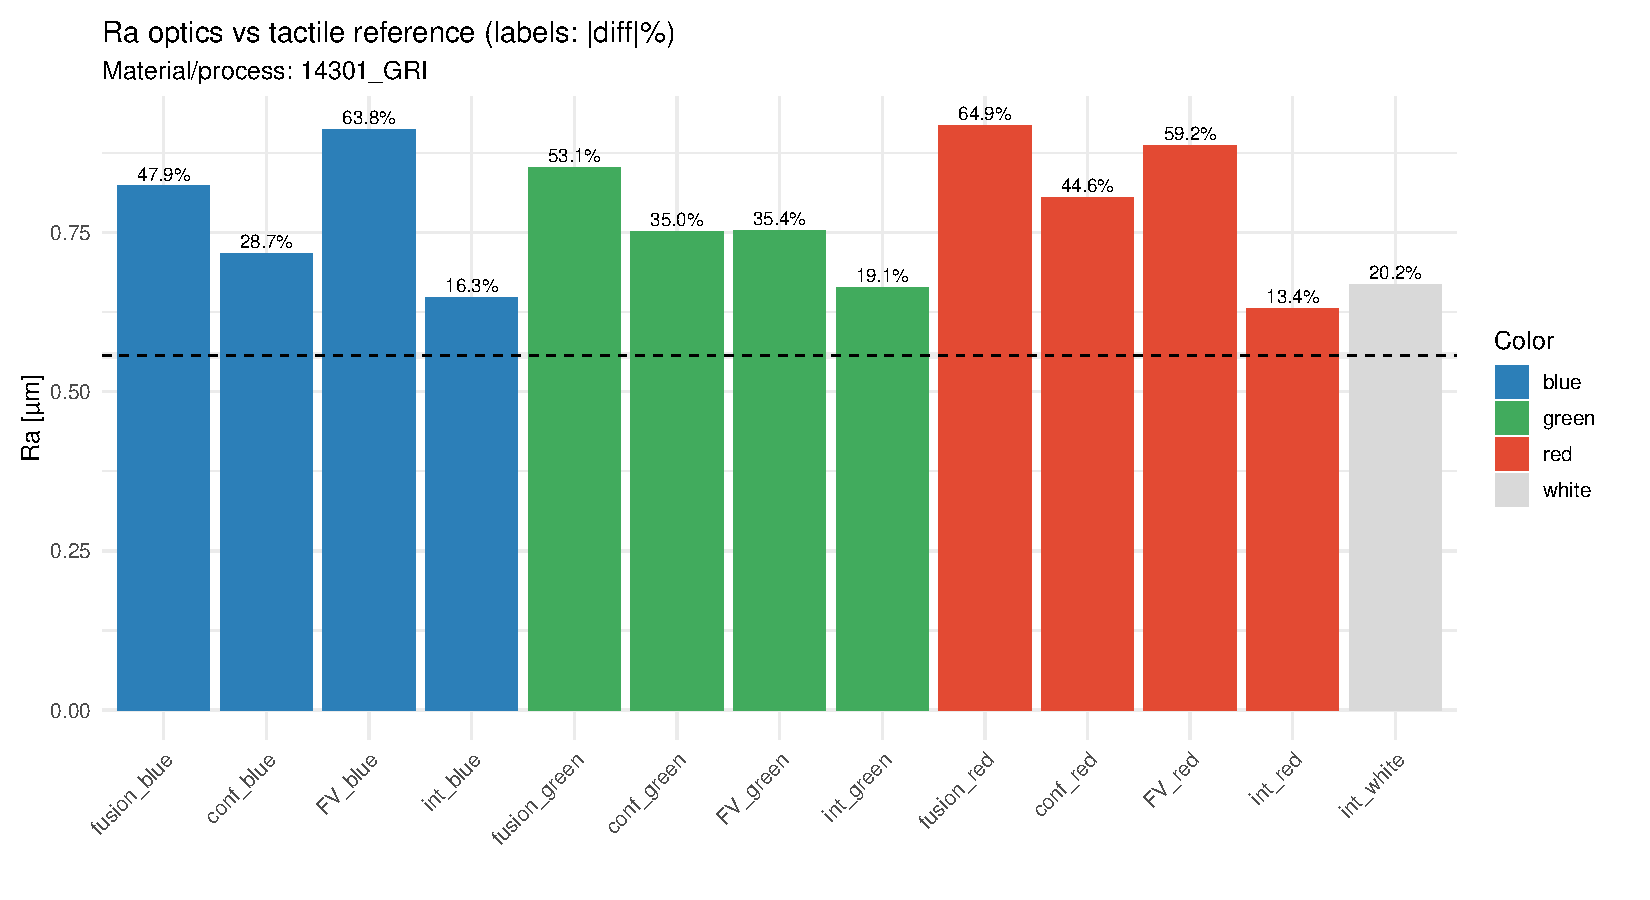
\includegraphics[width=\linewidth]{plots/ra_abs_14301_gri_optics_vs_tactile.pdf}
\end{minipage}
\begin{minipage}[t]{0.32\textwidth}\centering
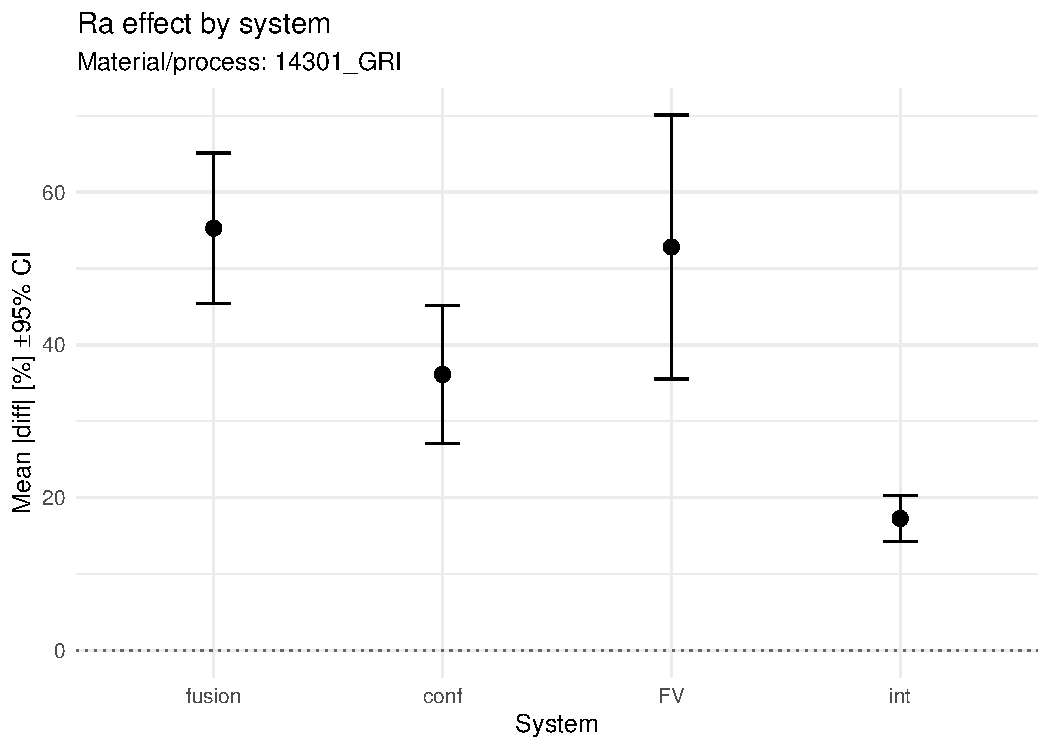
\includegraphics[width=\linewidth]{plots/ra_abs_14301_gri_effects_by_system.pdf}
\end{minipage}
\begin{minipage}[t]{0.32\textwidth}\centering
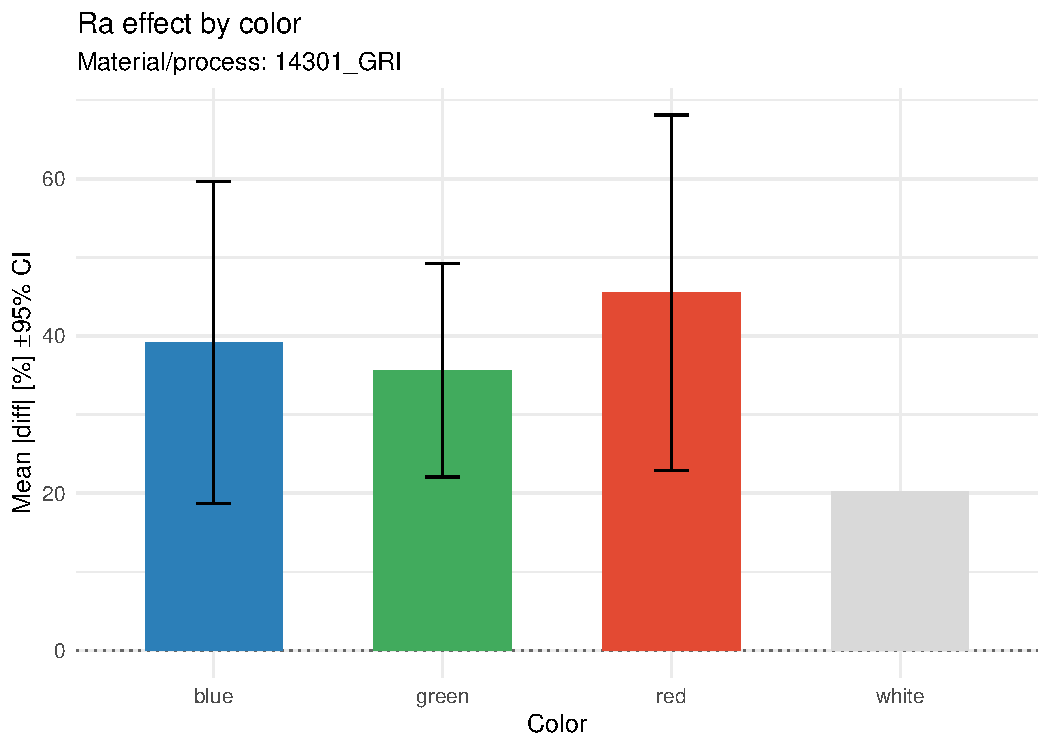
\includegraphics[width=\linewidth]{plots/ra_abs_14301_gri_effects_by_color.pdf}
\end{minipage}
\caption{RA — 14301\_gri — porównanie i efekty (|diff| \%)}
\end{figure}

\begin{figure}[H]\centering
\begin{minipage}[t]{0.32\textwidth}\centering
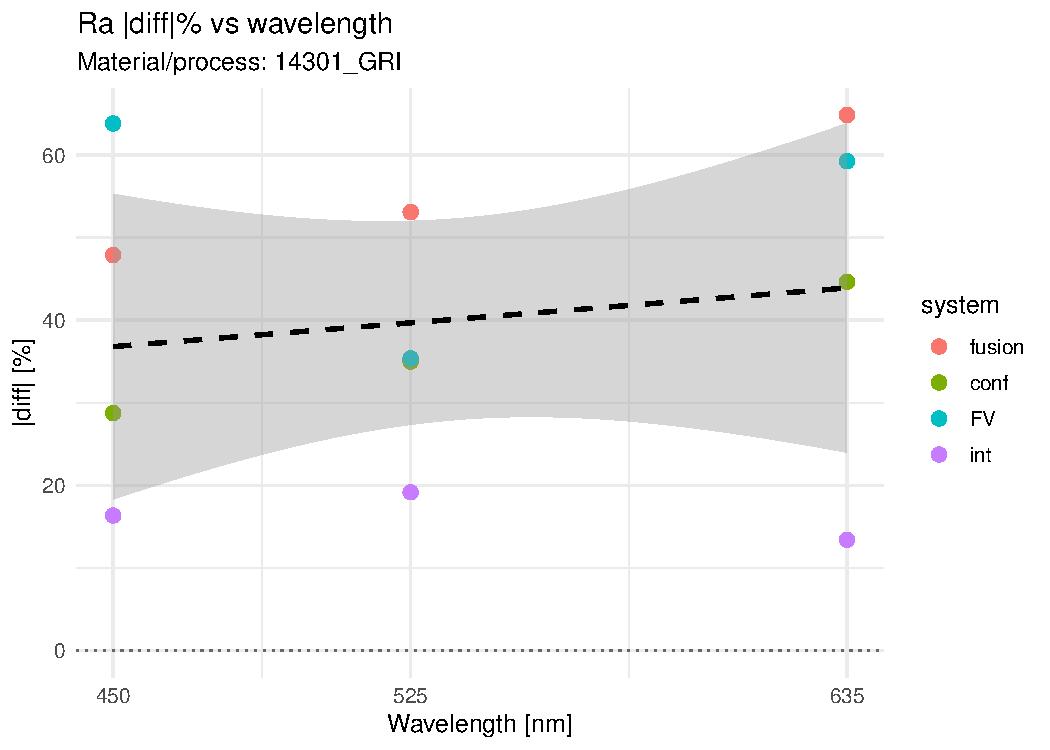
\includegraphics[width=\linewidth]{plots/ra_abs_14301_gri_diff_vs_wavelength.pdf}
\end{minipage}
\begin{minipage}[t]{0.32\textwidth}\centering
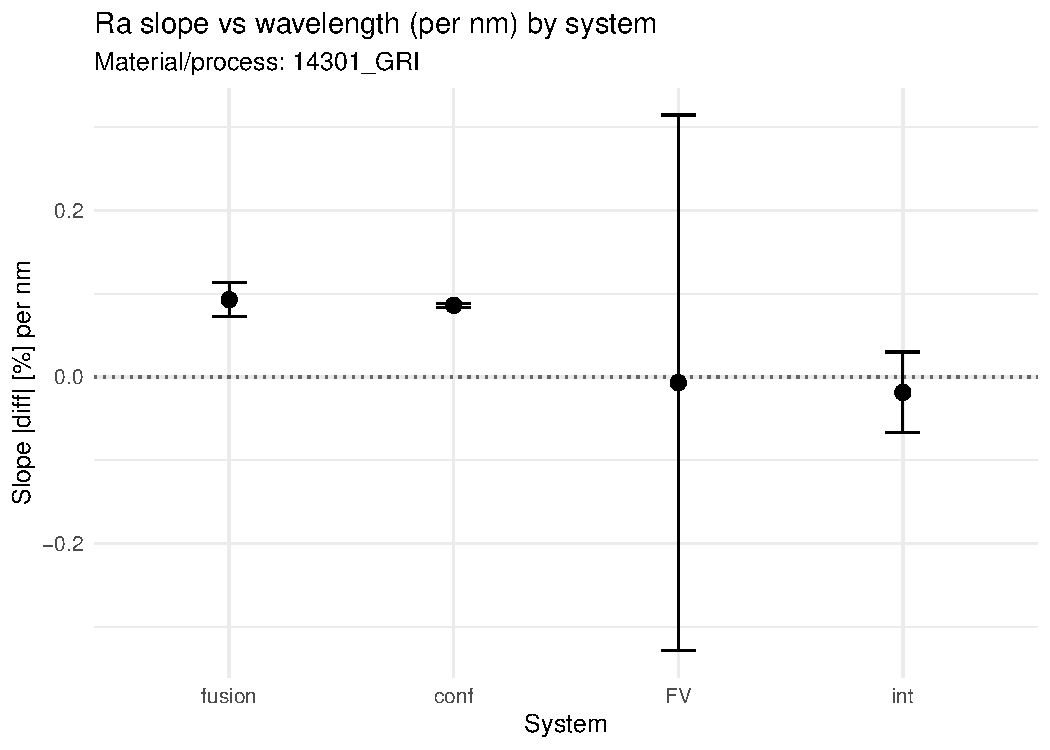
\includegraphics[width=\linewidth]{plots/ra_abs_14301_gri_slope_by_system_vs_nm.pdf}
\end{minipage}
\begin{minipage}[t]{0.32\textwidth}\centering
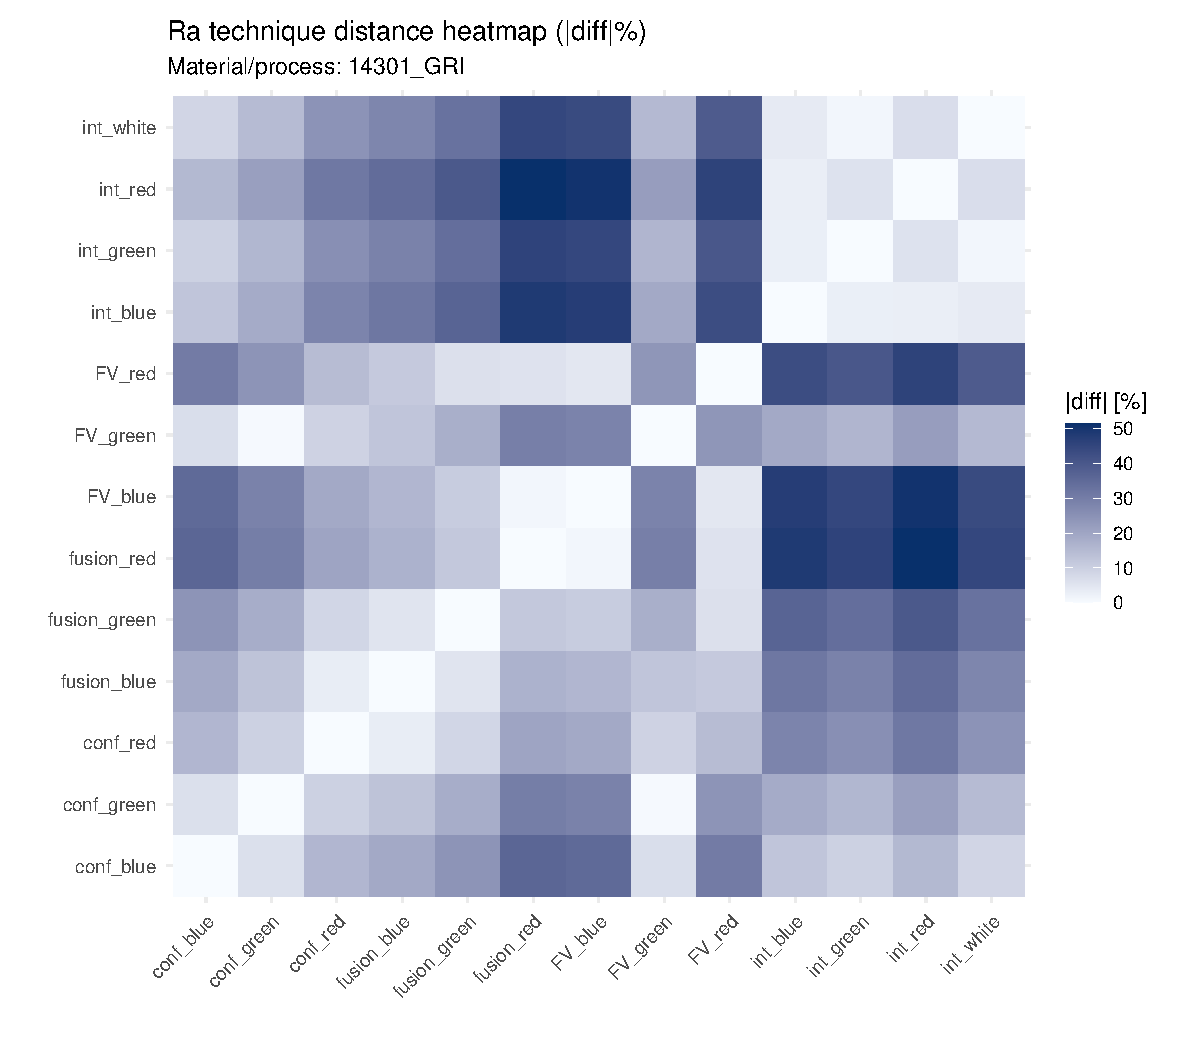
\includegraphics[width=\linewidth]{plots/ra_abs_14301_gri_tech_distance_heatmap.pdf}
\end{minipage}
\caption{RA — 14301\_gri — wavelength, nachylenia, odległości technik}
\end{figure}

\begin{figure}[H]\centering
\begin{minipage}[t]{0.32\textwidth}\centering
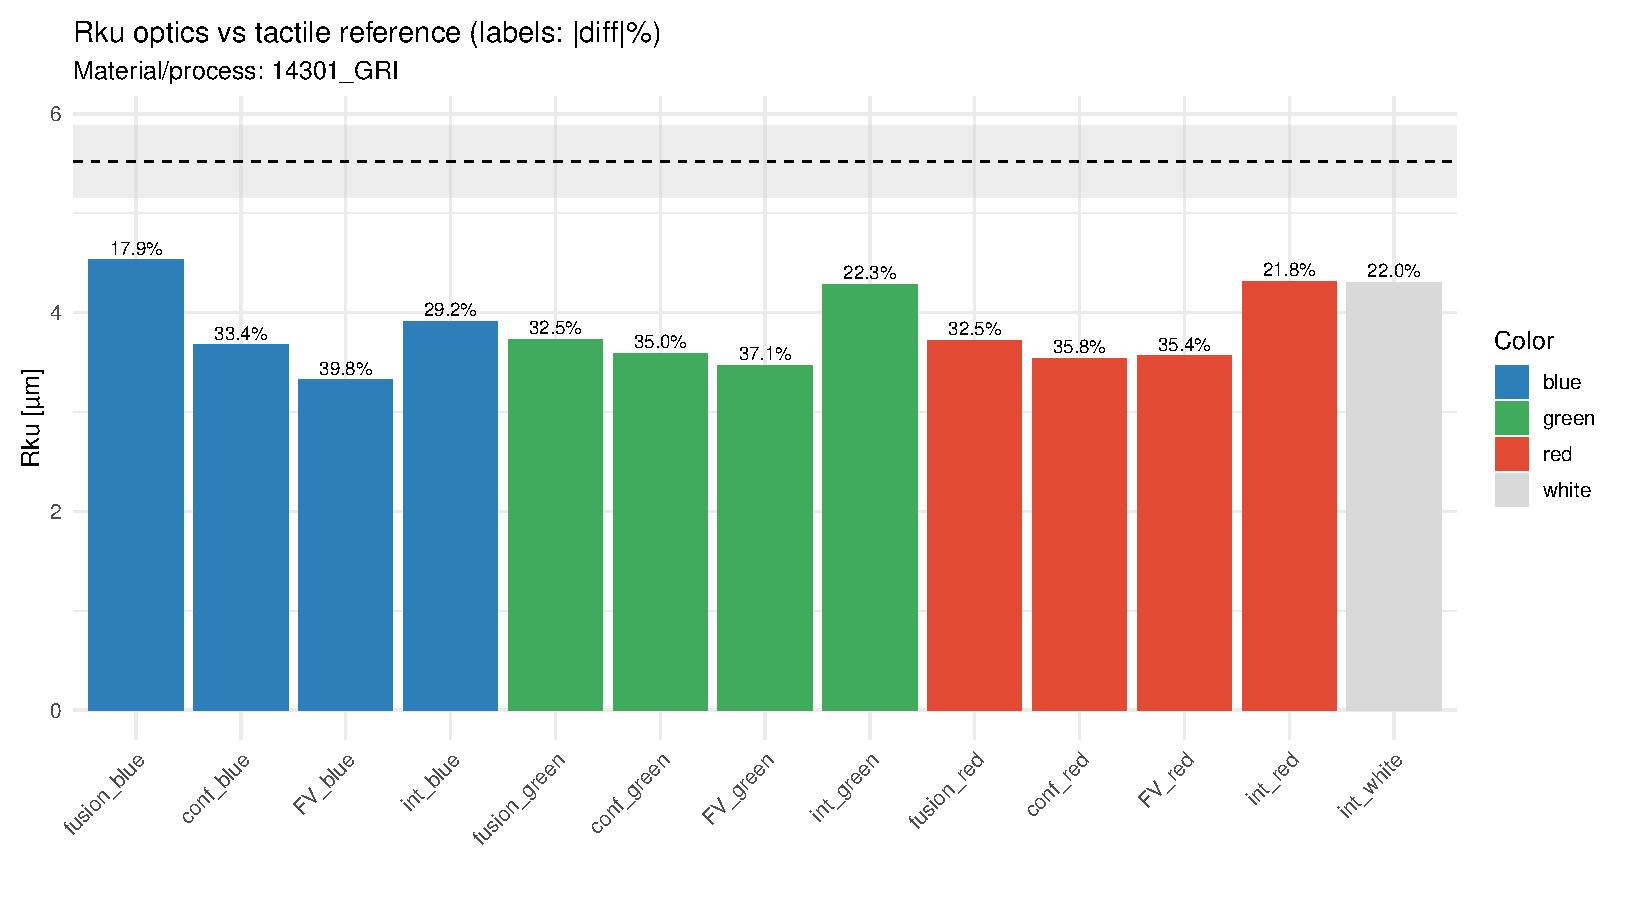
\includegraphics[width=\linewidth]{plots/rku_abs_14301_gri_optics_vs_tactile.pdf}
\end{minipage}
\begin{minipage}[t]{0.32\textwidth}\centering
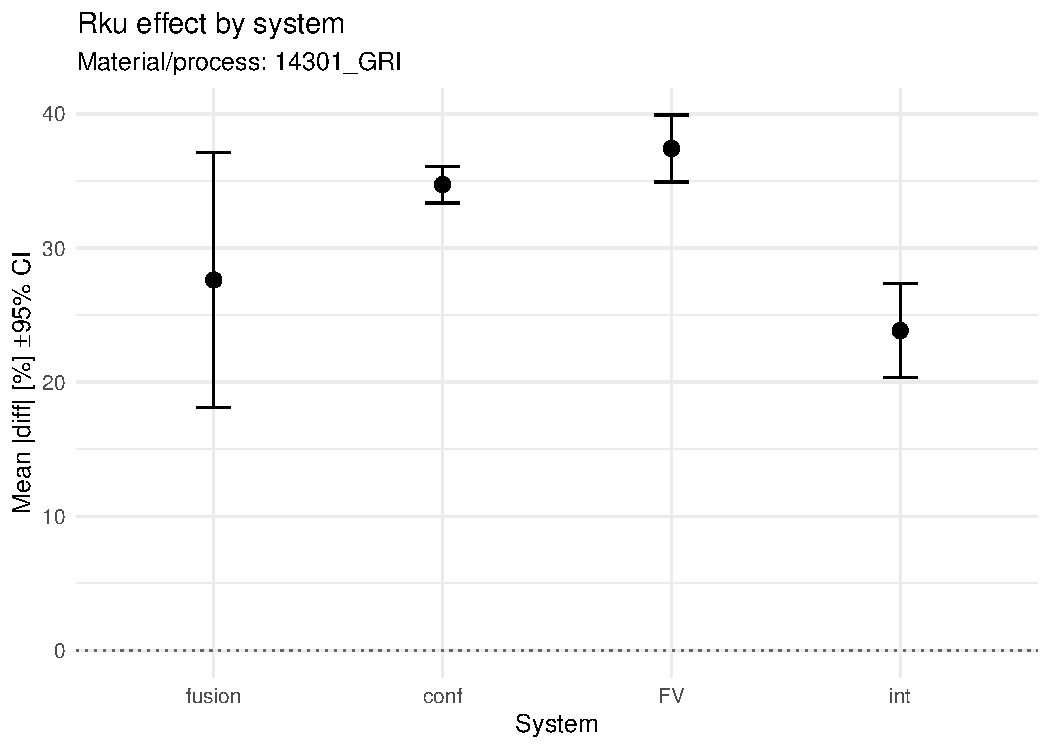
\includegraphics[width=\linewidth]{plots/rku_abs_14301_gri_effects_by_system.pdf}
\end{minipage}
\begin{minipage}[t]{0.32\textwidth}\centering
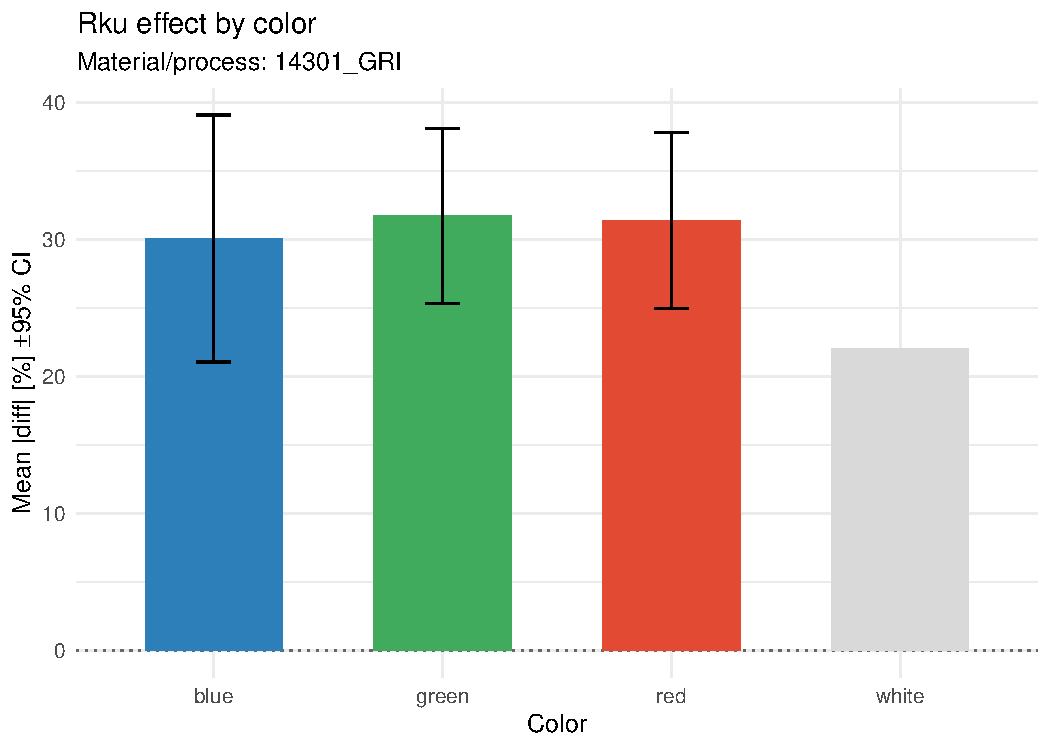
\includegraphics[width=\linewidth]{plots/rku_abs_14301_gri_effects_by_color.pdf}
\end{minipage}
\caption{RKU — 14301\_gri — porównanie i efekty (|diff| \%)}
\end{figure}

\begin{figure}[H]\centering
\begin{minipage}[t]{0.32\textwidth}\centering
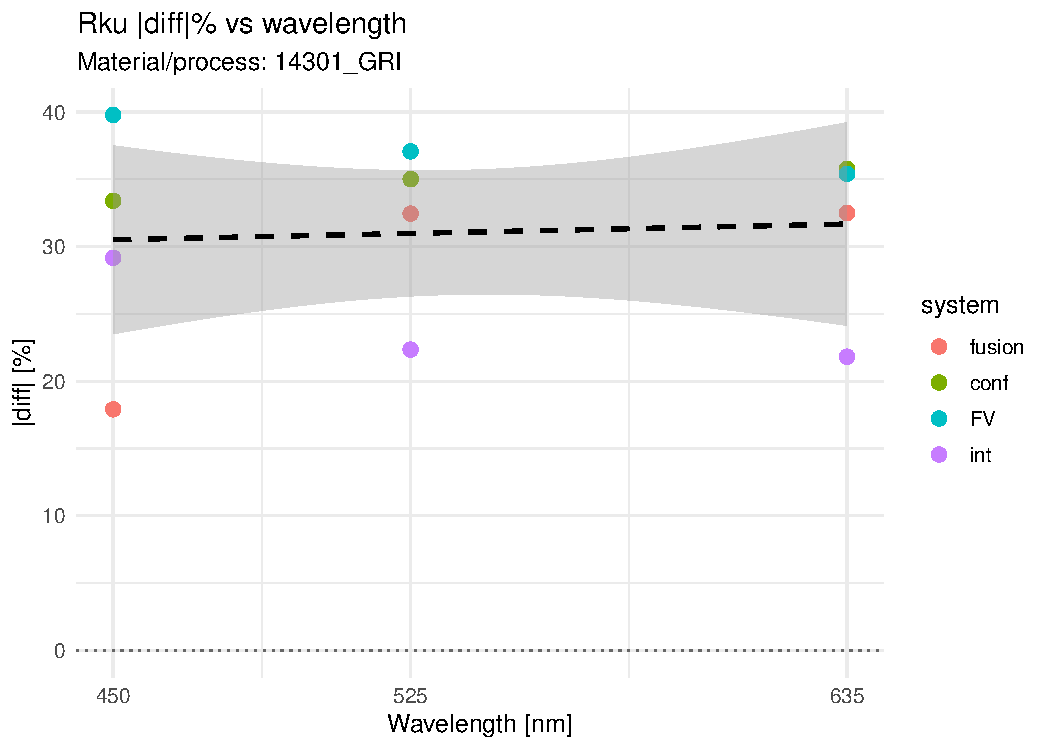
\includegraphics[width=\linewidth]{plots/rku_abs_14301_gri_diff_vs_wavelength.pdf}
\end{minipage}
\begin{minipage}[t]{0.32\textwidth}\centering
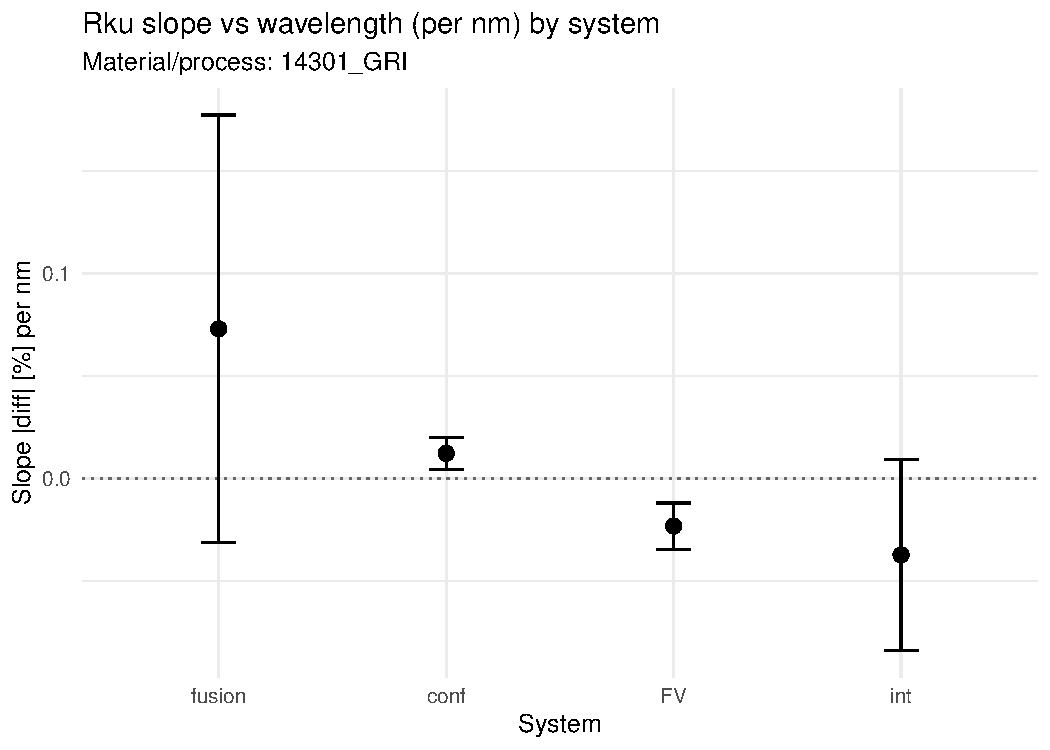
\includegraphics[width=\linewidth]{plots/rku_abs_14301_gri_slope_by_system_vs_nm.pdf}
\end{minipage}
\begin{minipage}[t]{0.32\textwidth}\centering
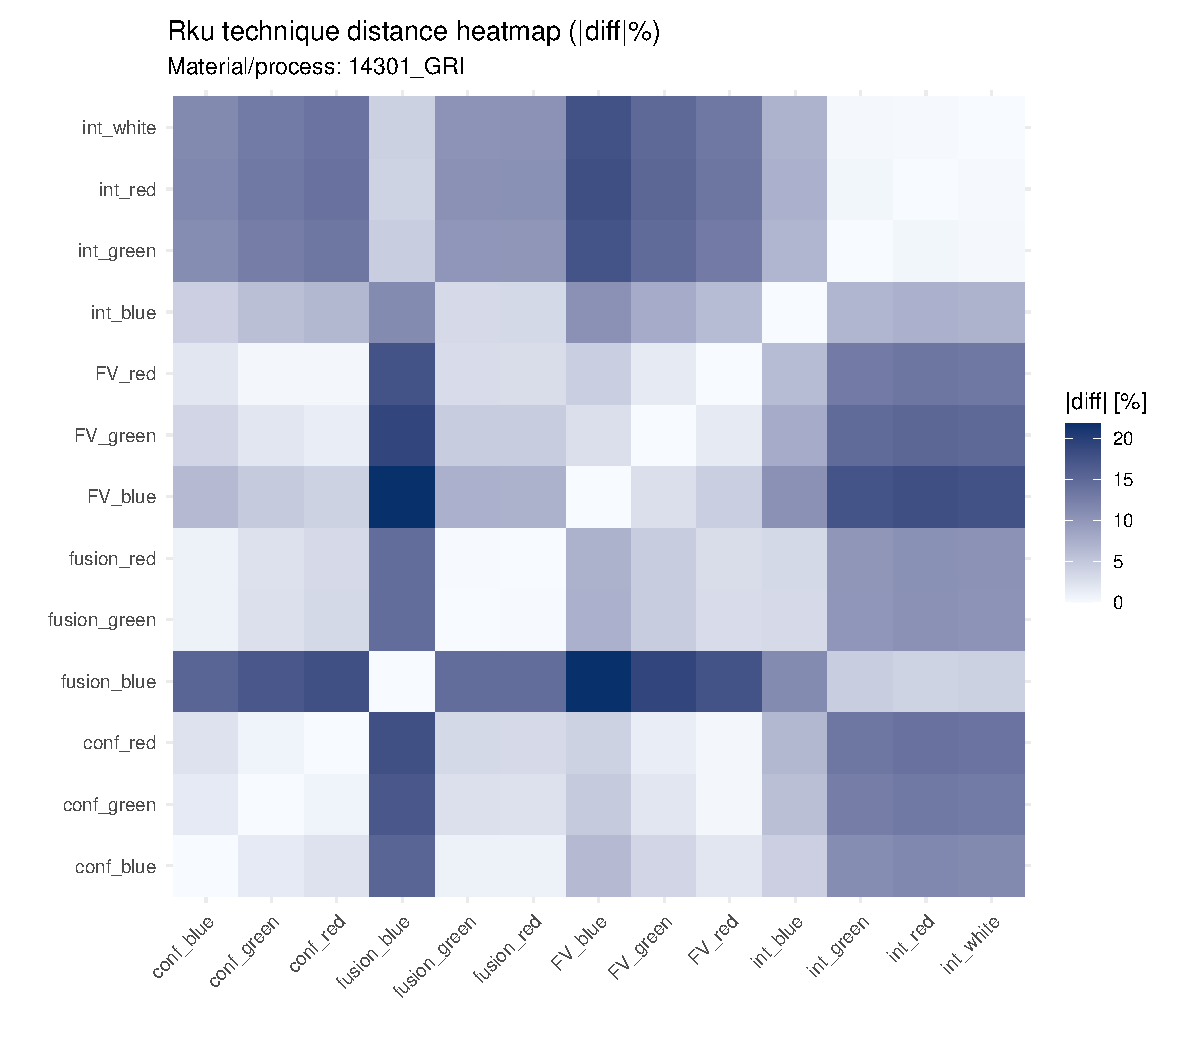
\includegraphics[width=\linewidth]{plots/rku_abs_14301_gri_tech_distance_heatmap.pdf}
\end{minipage}
\caption{RKU — 14301\_gri — wavelength, nachylenia, odległości technik}
\end{figure}

\begin{figure}[H]\centering
\begin{minipage}[t]{0.32\textwidth}\centering
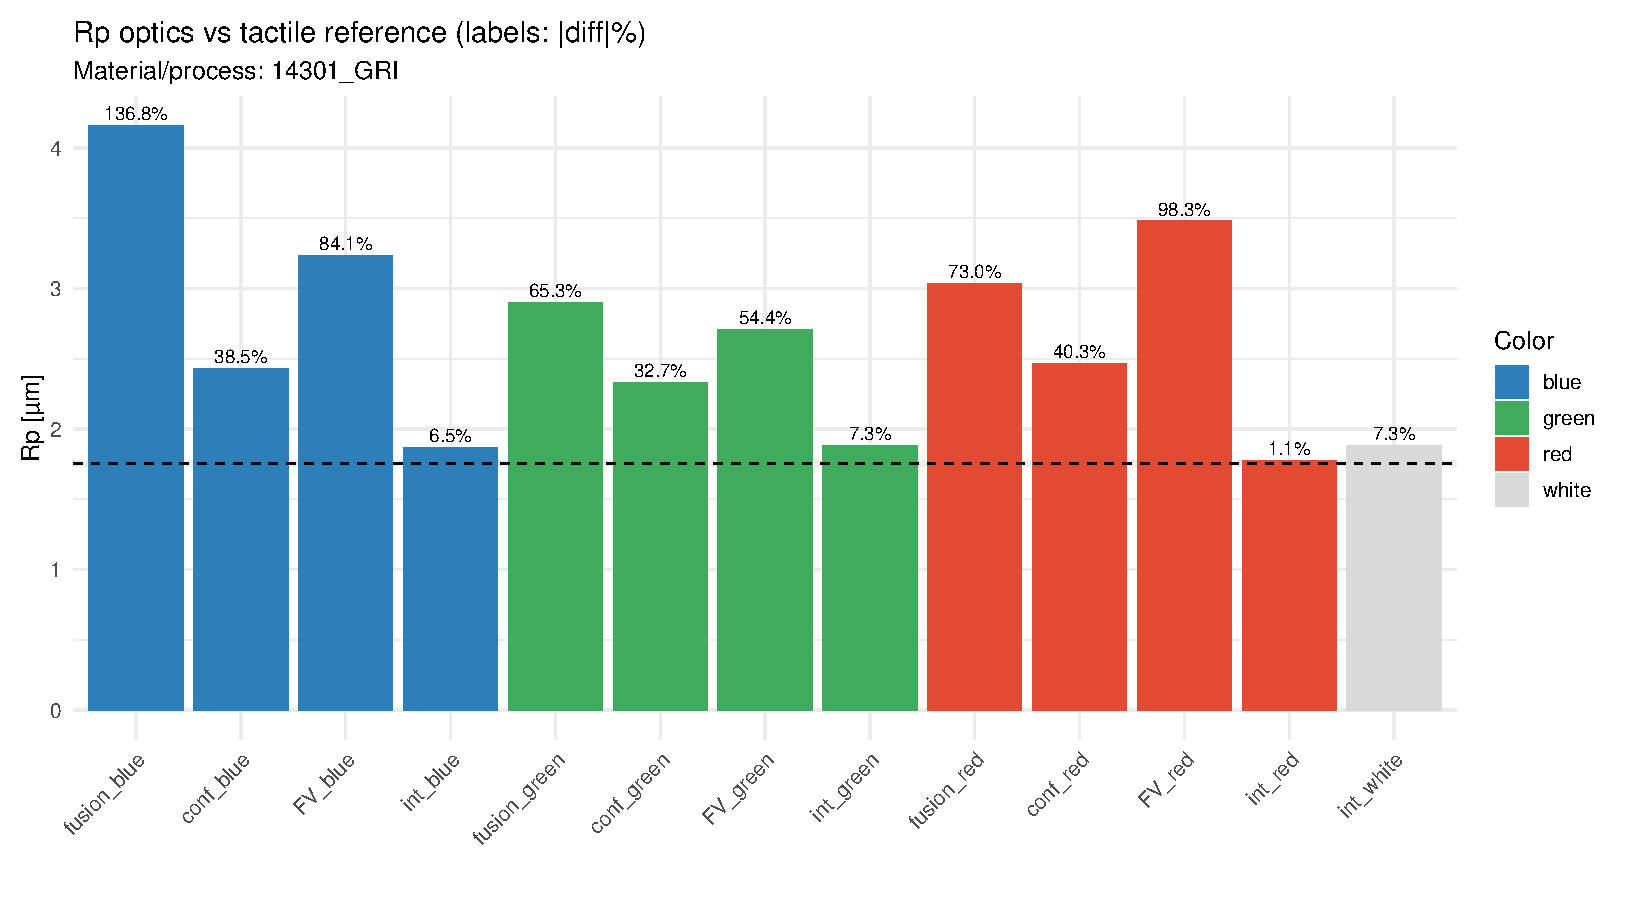
\includegraphics[width=\linewidth]{plots/rp_abs_14301_gri_optics_vs_tactile.pdf}
\end{minipage}
\begin{minipage}[t]{0.32\textwidth}\centering
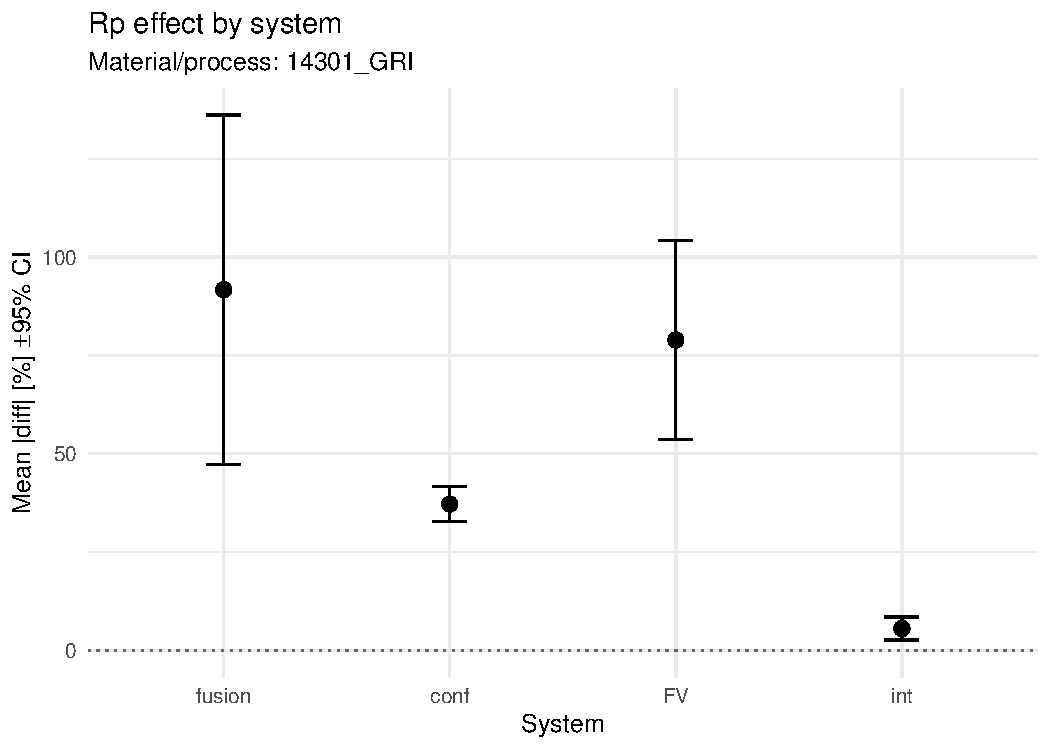
\includegraphics[width=\linewidth]{plots/rp_abs_14301_gri_effects_by_system.pdf}
\end{minipage}
\begin{minipage}[t]{0.32\textwidth}\centering
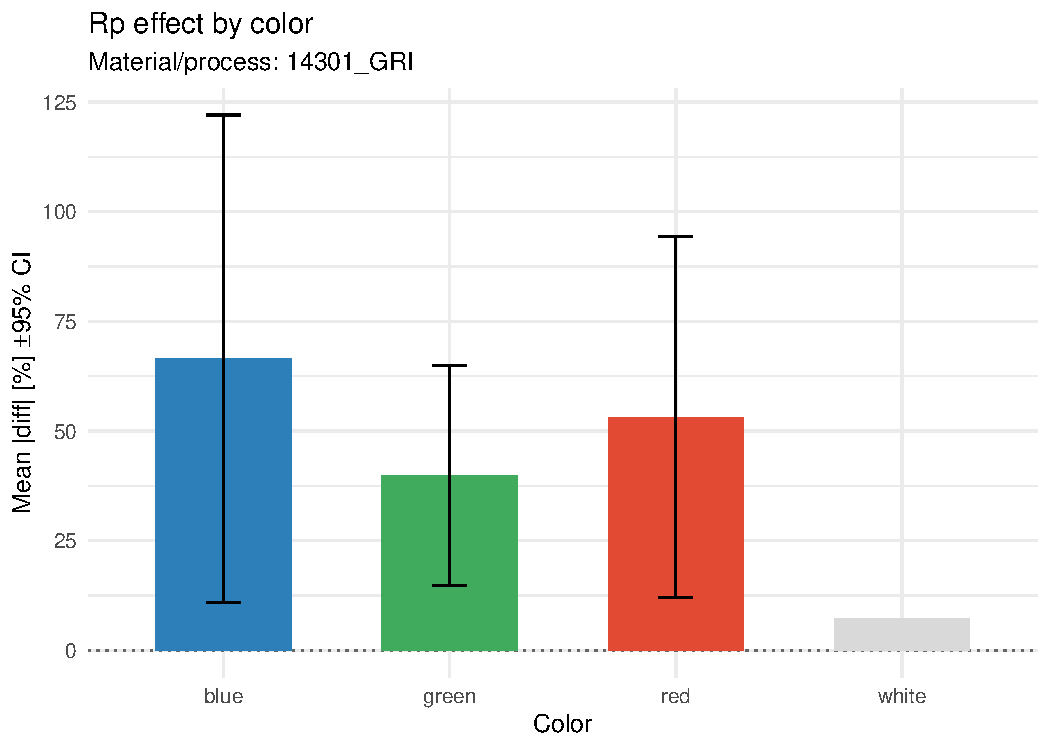
\includegraphics[width=\linewidth]{plots/rp_abs_14301_gri_effects_by_color.pdf}
\end{minipage}
\caption{RP — 14301\_gri — porównanie i efekty (|diff| \%)}
\end{figure}

\begin{figure}[H]\centering
\begin{minipage}[t]{0.32\textwidth}\centering
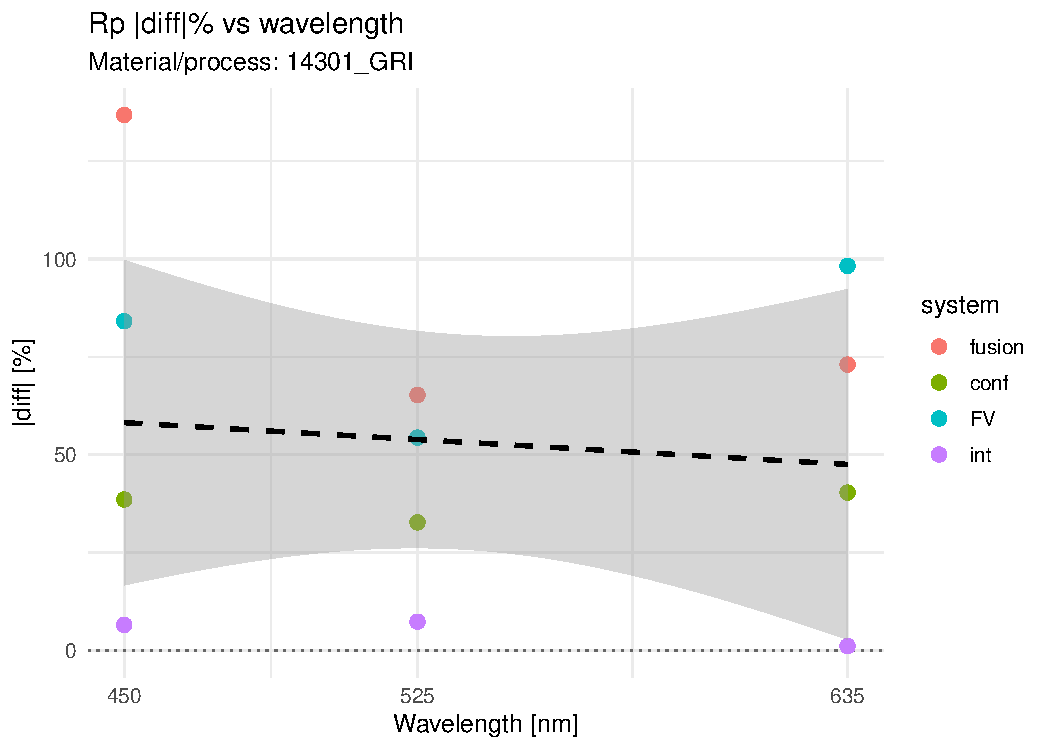
\includegraphics[width=\linewidth]{plots/rp_abs_14301_gri_diff_vs_wavelength.pdf}
\end{minipage}
\begin{minipage}[t]{0.32\textwidth}\centering
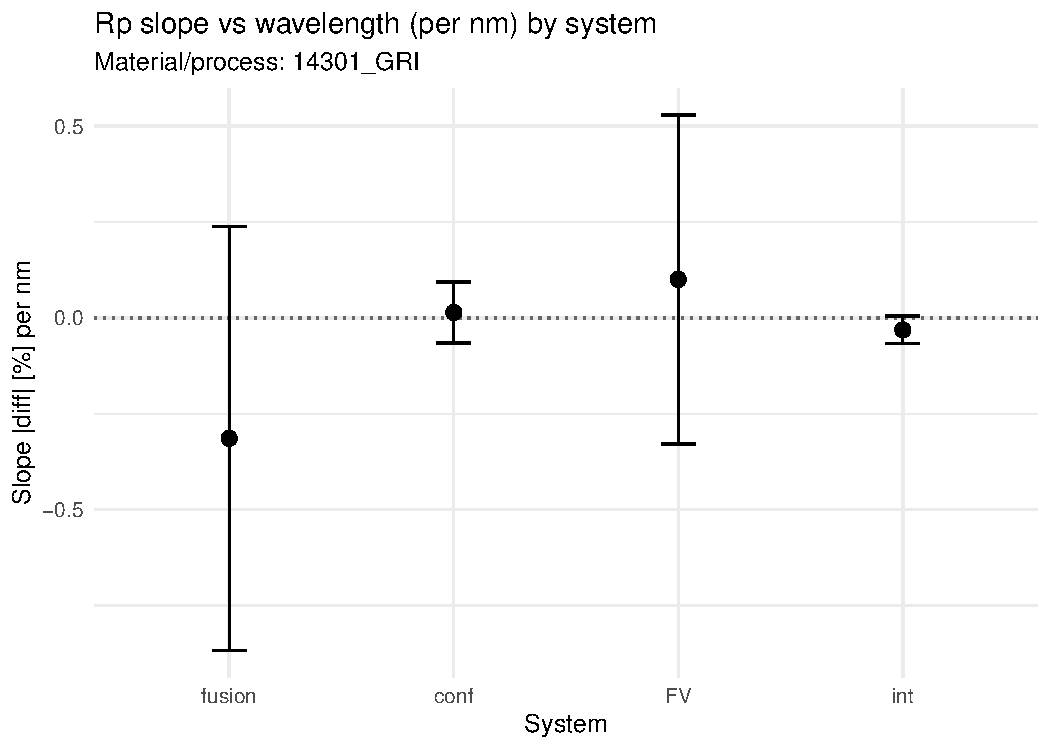
\includegraphics[width=\linewidth]{plots/rp_abs_14301_gri_slope_by_system_vs_nm.pdf}
\end{minipage}
\begin{minipage}[t]{0.32\textwidth}\centering
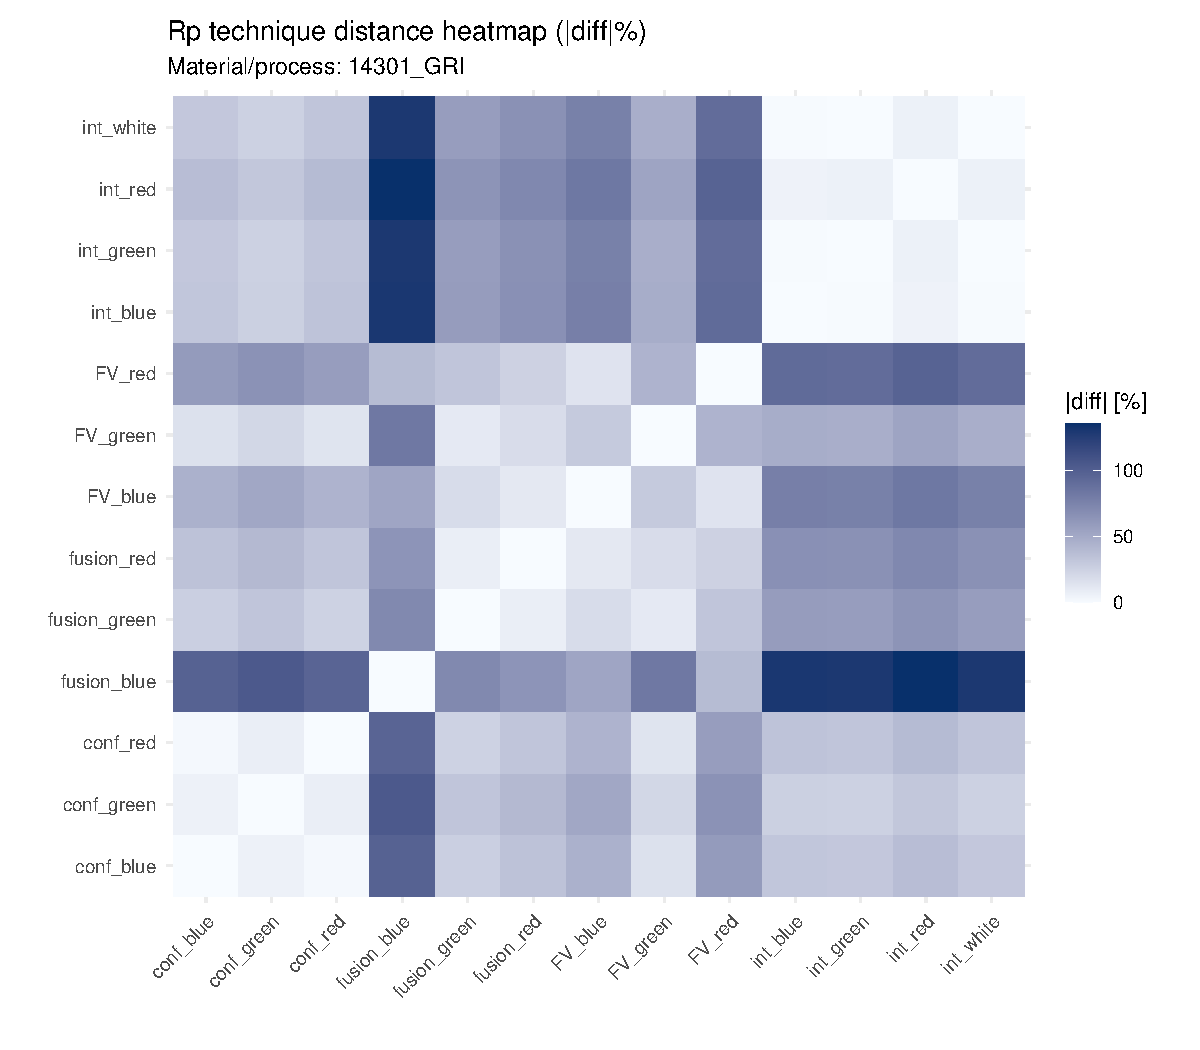
\includegraphics[width=\linewidth]{plots/rp_abs_14301_gri_tech_distance_heatmap.pdf}
\end{minipage}
\caption{RP — 14301\_gri — wavelength, nachylenia, odległości technik}
\end{figure}

\begin{figure}[H]\centering
\begin{minipage}[t]{0.32\textwidth}\centering
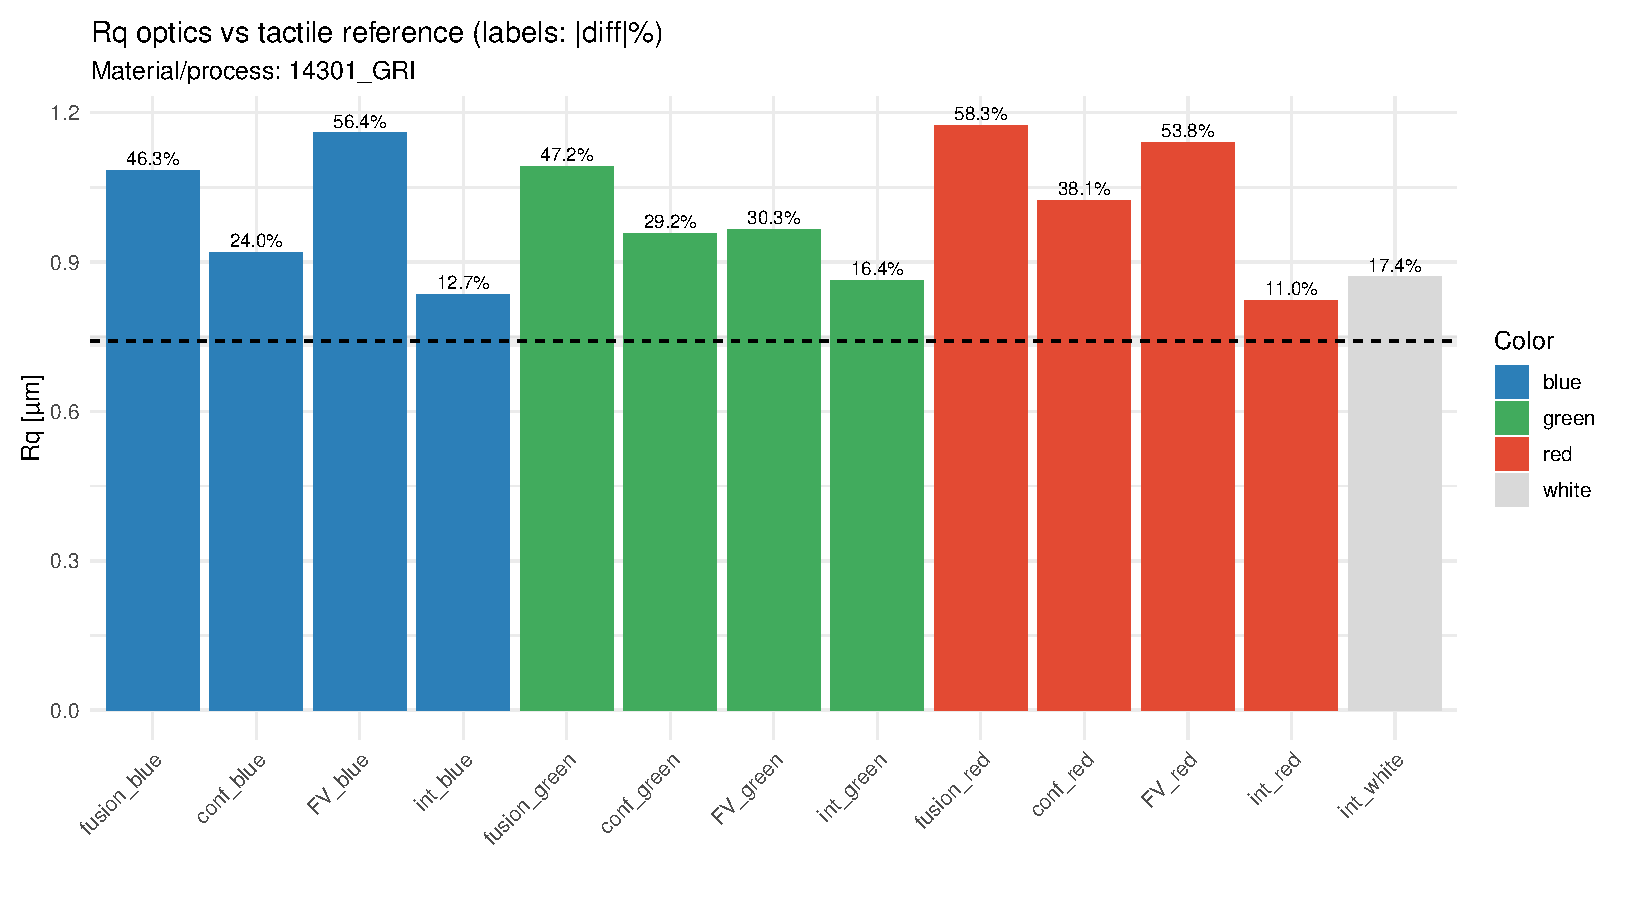
\includegraphics[width=\linewidth]{plots/rq_abs_14301_gri_optics_vs_tactile.pdf}
\end{minipage}
\begin{minipage}[t]{0.32\textwidth}\centering
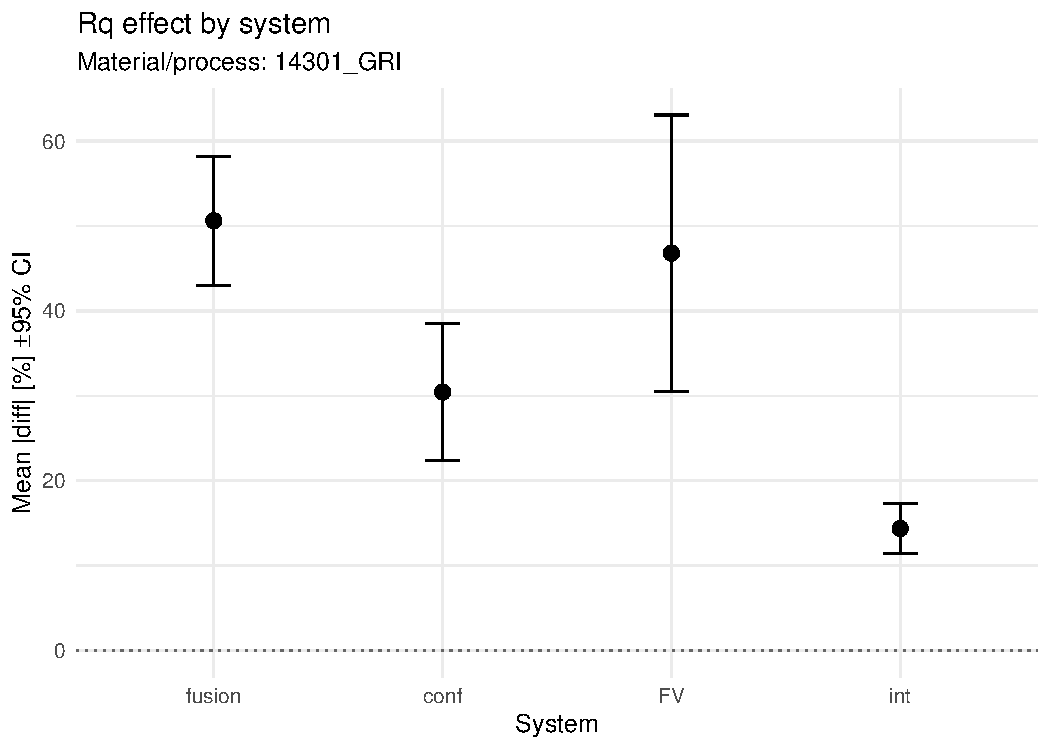
\includegraphics[width=\linewidth]{plots/rq_abs_14301_gri_effects_by_system.pdf}
\end{minipage}
\begin{minipage}[t]{0.32\textwidth}\centering
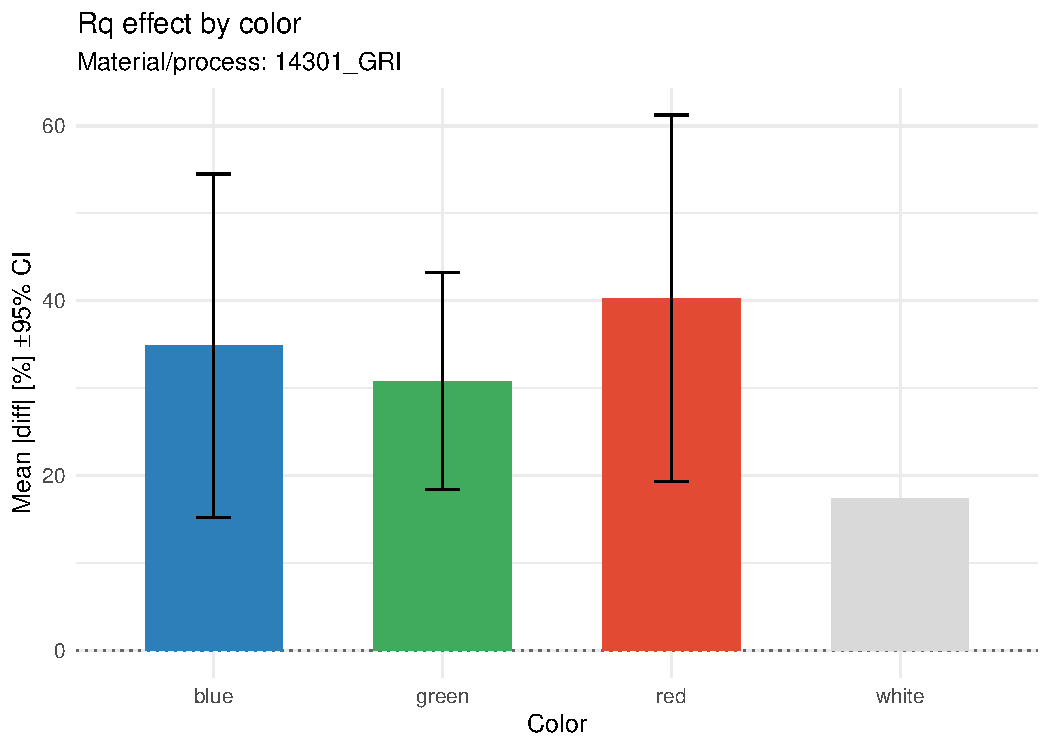
\includegraphics[width=\linewidth]{plots/rq_abs_14301_gri_effects_by_color.pdf}
\end{minipage}
\caption{RQ — 14301\_gri — porównanie i efekty (|diff| \%)}
\end{figure}

\begin{figure}[H]\centering
\begin{minipage}[t]{0.32\textwidth}\centering
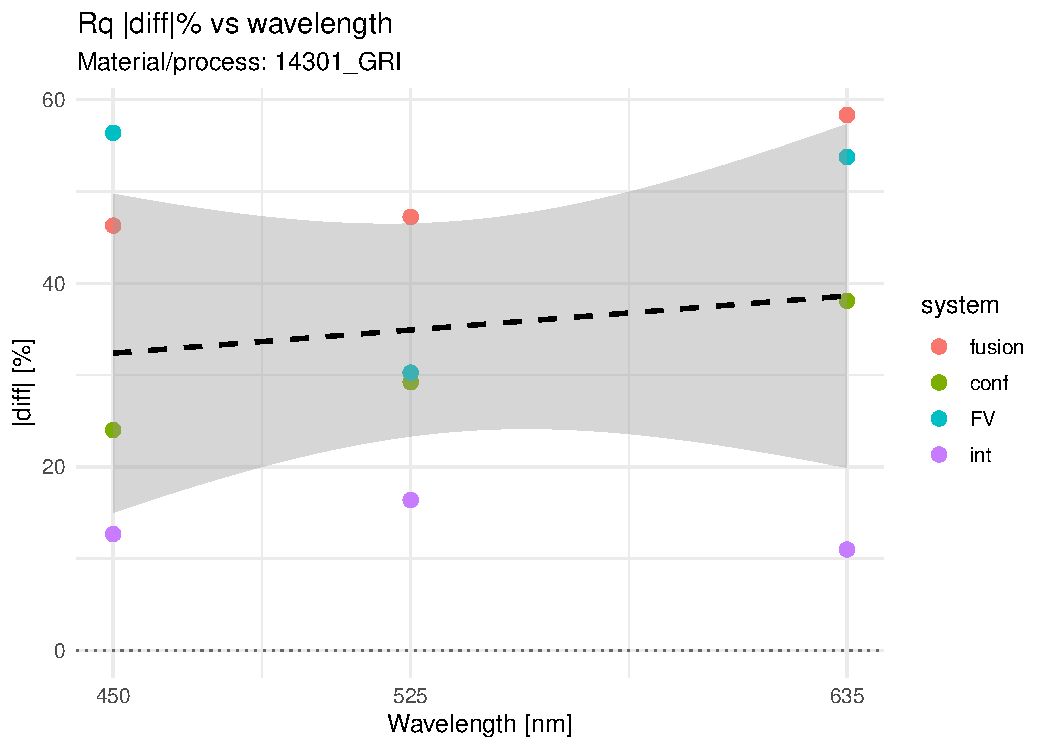
\includegraphics[width=\linewidth]{plots/rq_abs_14301_gri_diff_vs_wavelength.pdf}
\end{minipage}
\begin{minipage}[t]{0.32\textwidth}\centering
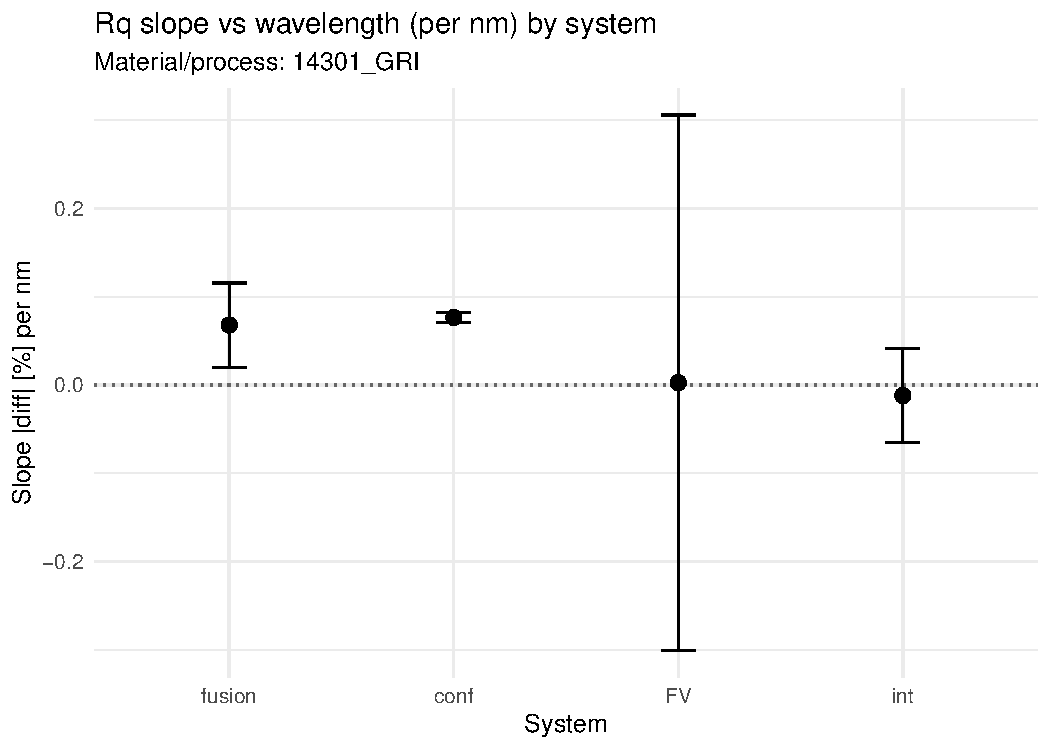
\includegraphics[width=\linewidth]{plots/rq_abs_14301_gri_slope_by_system_vs_nm.pdf}
\end{minipage}
\begin{minipage}[t]{0.32\textwidth}\centering
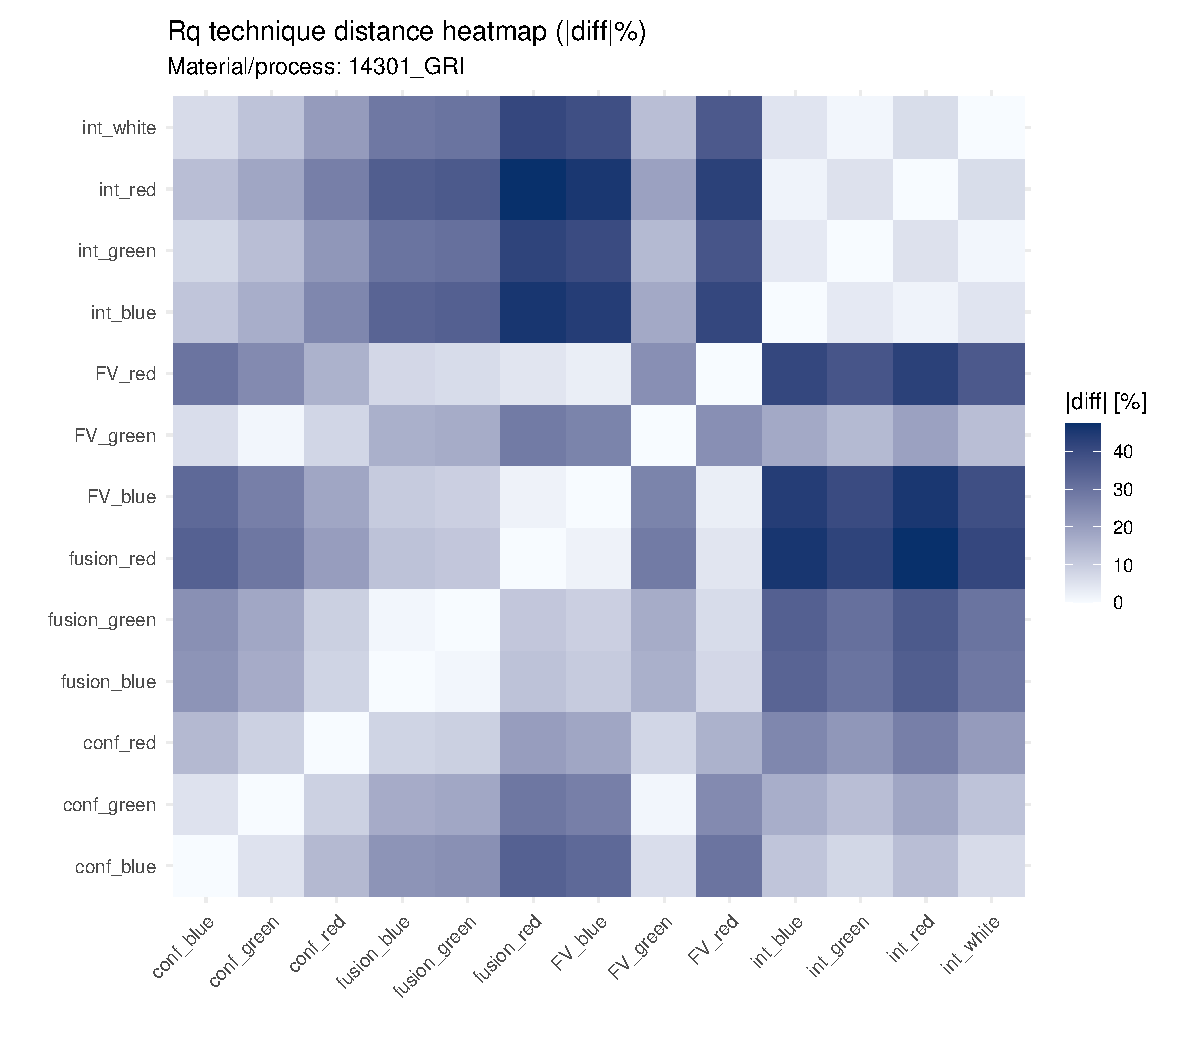
\includegraphics[width=\linewidth]{plots/rq_abs_14301_gri_tech_distance_heatmap.pdf}
\end{minipage}
\caption{RQ — 14301\_gri — wavelength, nachylenia, odległości technik}
\end{figure}

\begin{figure}[H]\centering
\begin{minipage}[t]{0.32\textwidth}\centering
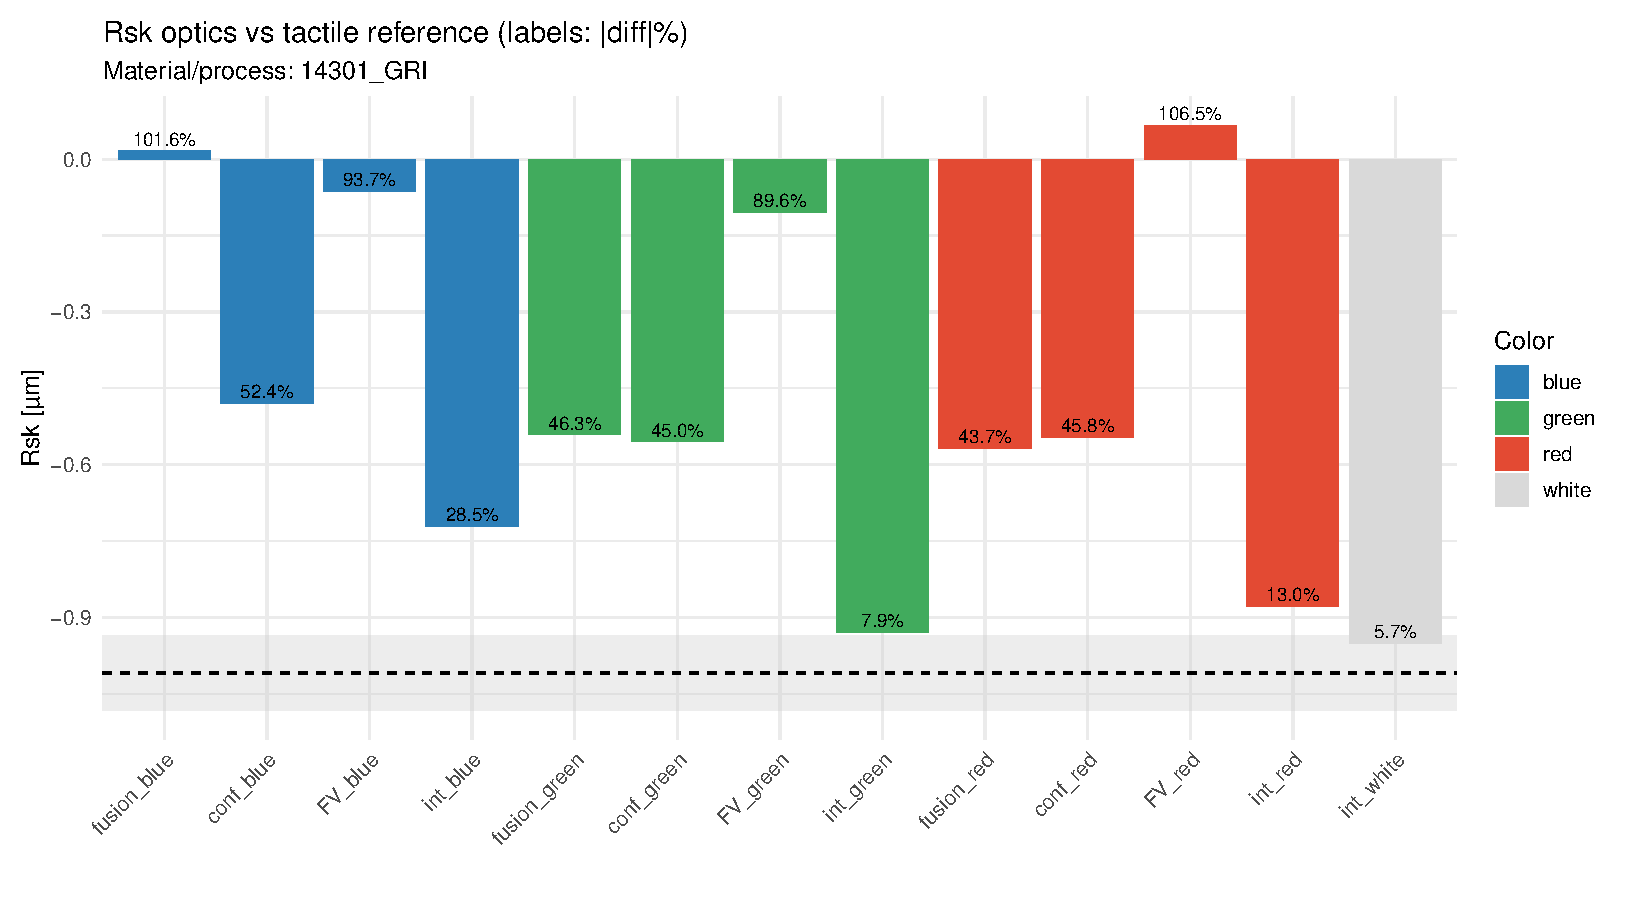
\includegraphics[width=\linewidth]{plots/rsk_abs_14301_gri_optics_vs_tactile.pdf}
\end{minipage}
\begin{minipage}[t]{0.32\textwidth}\centering
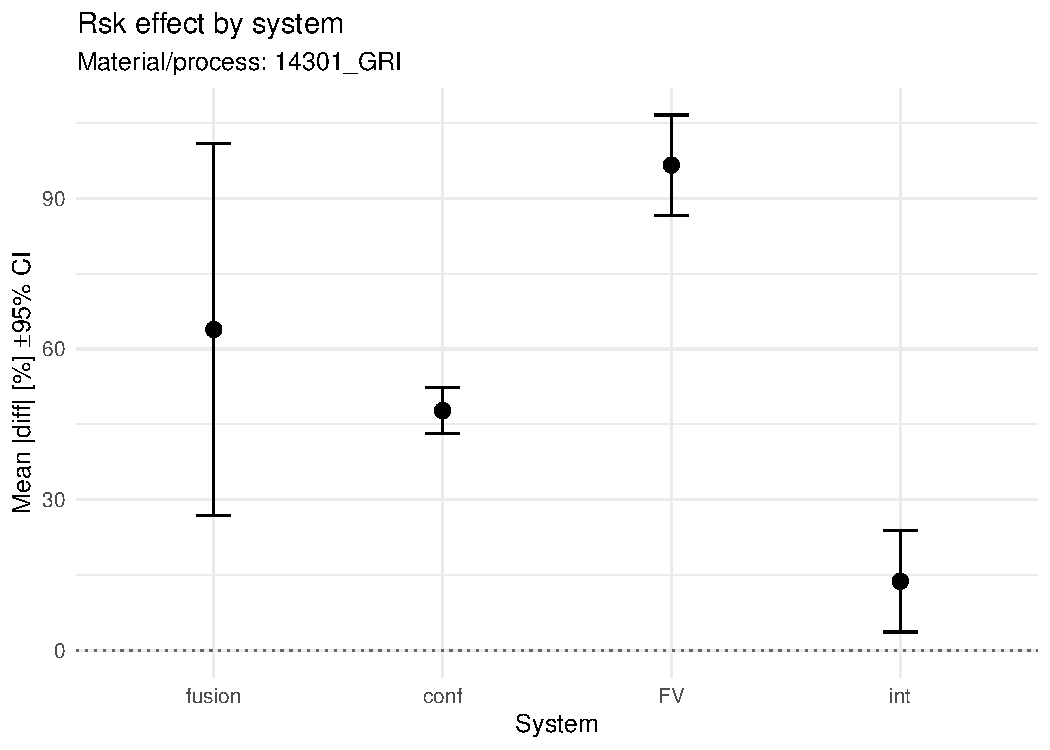
\includegraphics[width=\linewidth]{plots/rsk_abs_14301_gri_effects_by_system.pdf}
\end{minipage}
\begin{minipage}[t]{0.32\textwidth}\centering
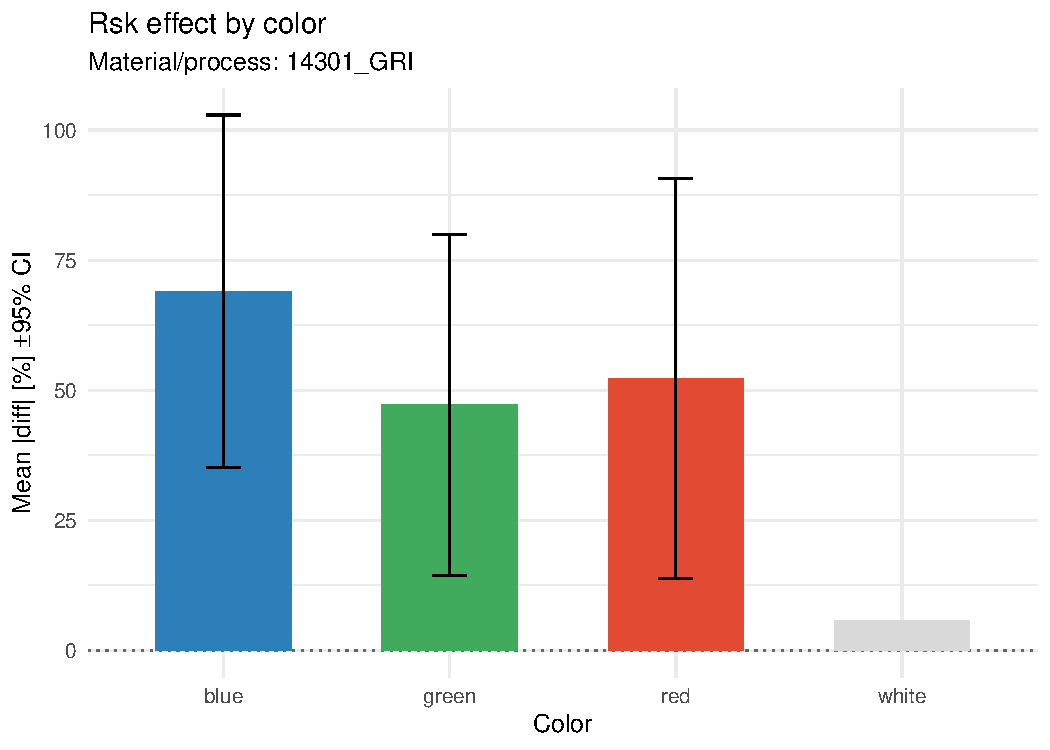
\includegraphics[width=\linewidth]{plots/rsk_abs_14301_gri_effects_by_color.pdf}
\end{minipage}
\caption{RSK — 14301\_gri — porównanie i efekty (|diff| \%)}
\end{figure}

\begin{figure}[H]\centering
\begin{minipage}[t]{0.32\textwidth}\centering
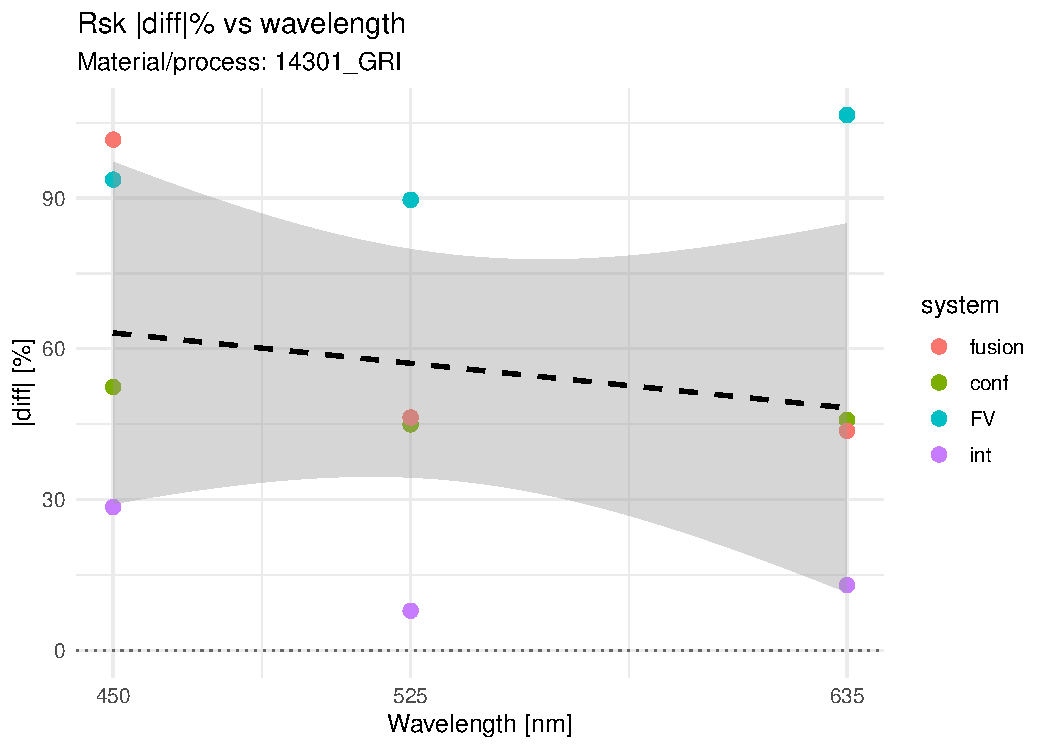
\includegraphics[width=\linewidth]{plots/rsk_abs_14301_gri_diff_vs_wavelength.pdf}
\end{minipage}
\begin{minipage}[t]{0.32\textwidth}\centering
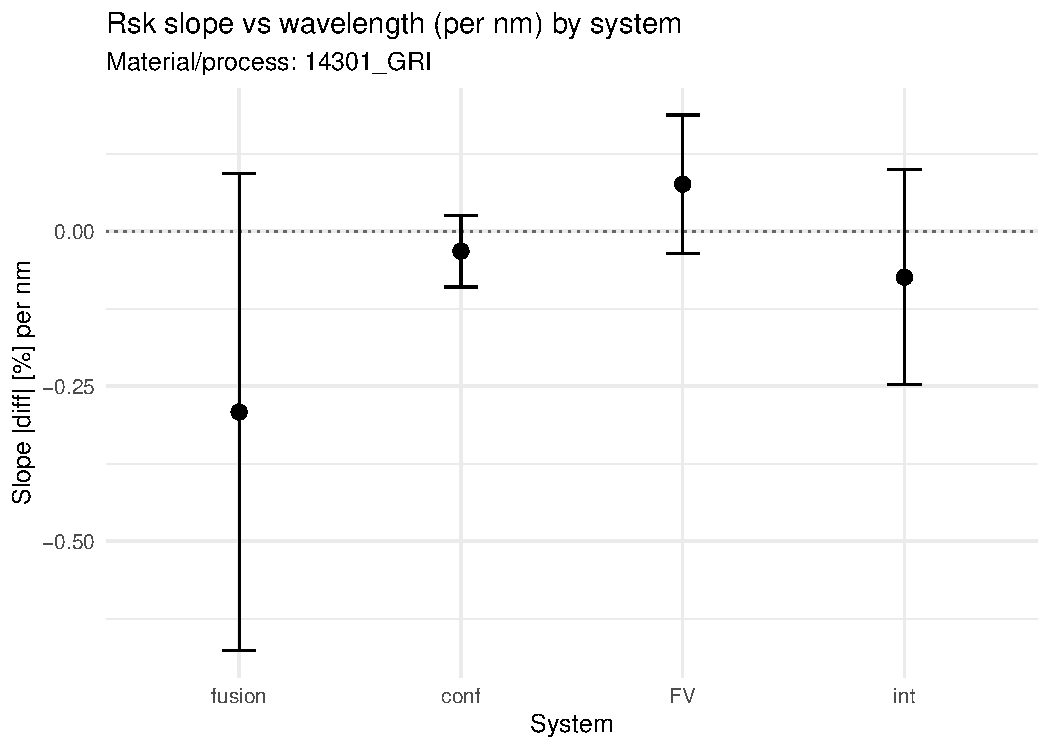
\includegraphics[width=\linewidth]{plots/rsk_abs_14301_gri_slope_by_system_vs_nm.pdf}
\end{minipage}
\begin{minipage}[t]{0.32\textwidth}\centering
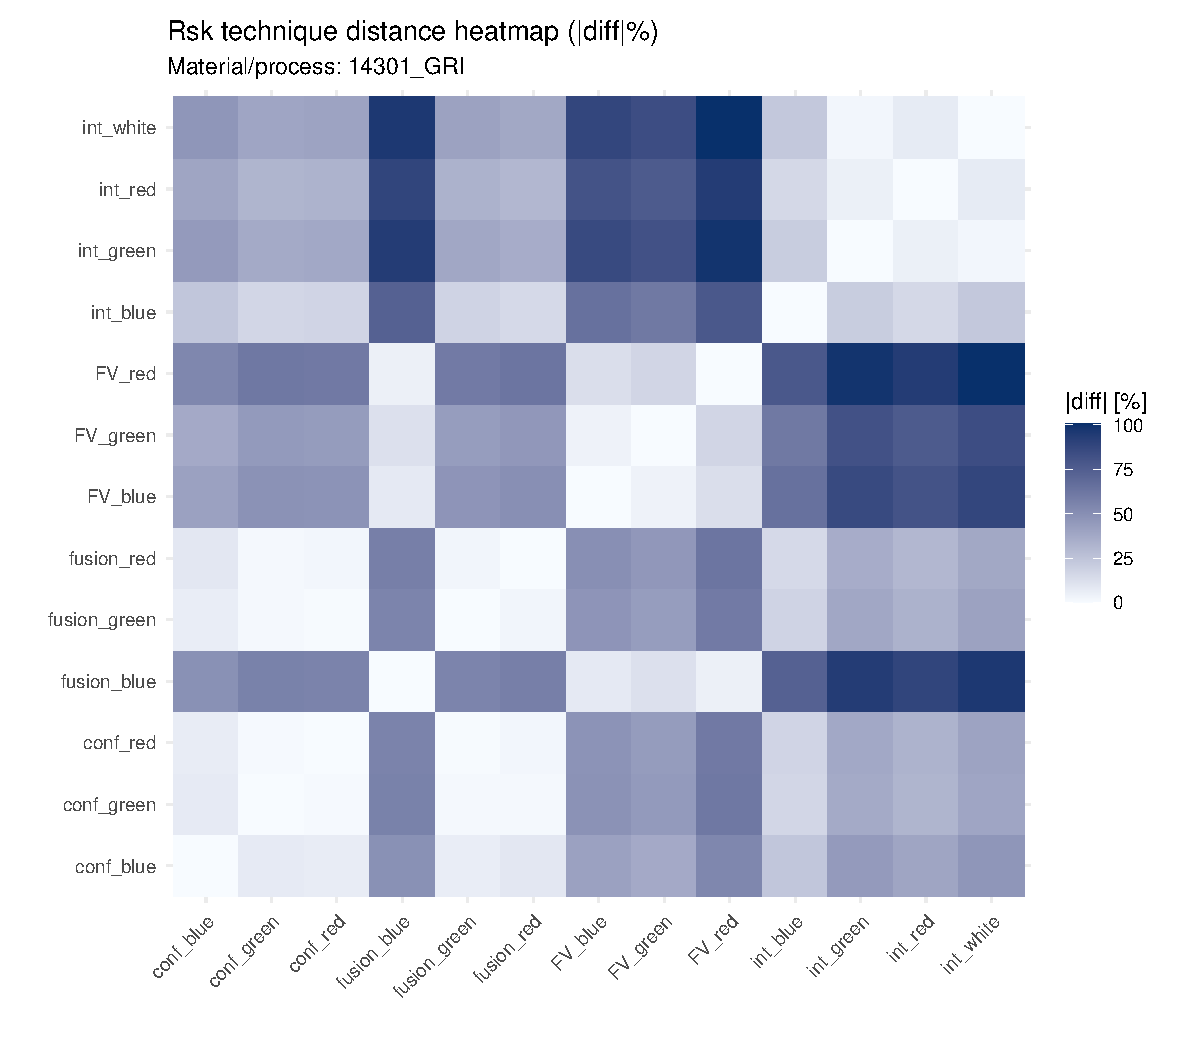
\includegraphics[width=\linewidth]{plots/rsk_abs_14301_gri_tech_distance_heatmap.pdf}
\end{minipage}
\caption{RSK — 14301\_gri — wavelength, nachylenia, odległości technik}
\end{figure}

\begin{figure}[H]\centering
\begin{minipage}[t]{0.32\textwidth}\centering
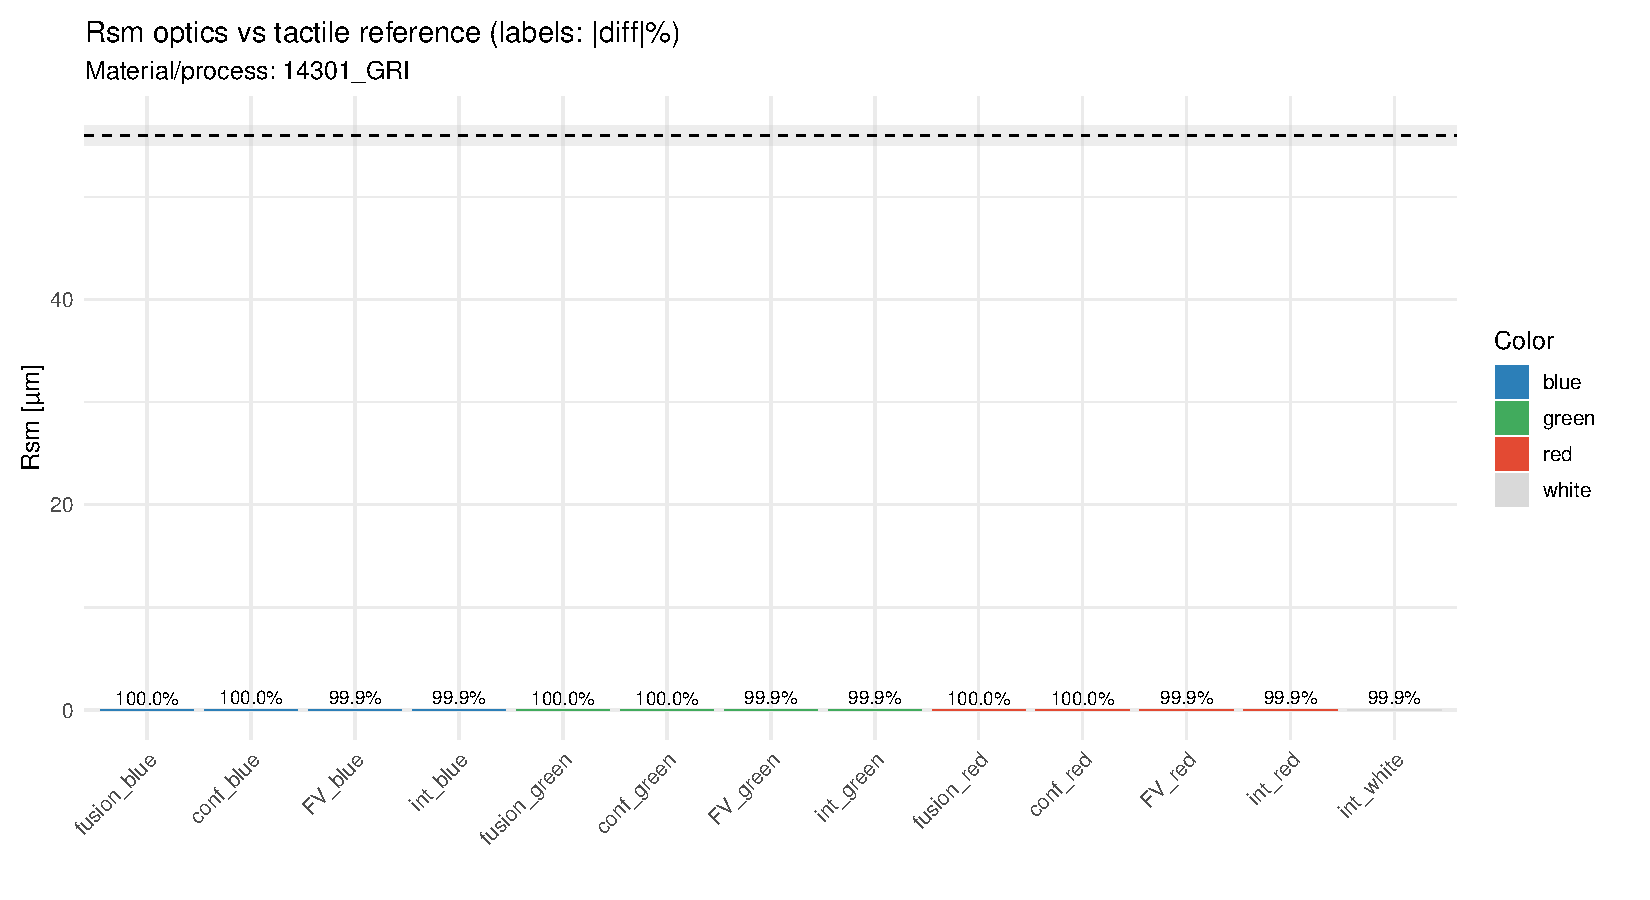
\includegraphics[width=\linewidth]{plots/rsm_abs_14301_gri_optics_vs_tactile.pdf}
\end{minipage}
\begin{minipage}[t]{0.32\textwidth}\centering
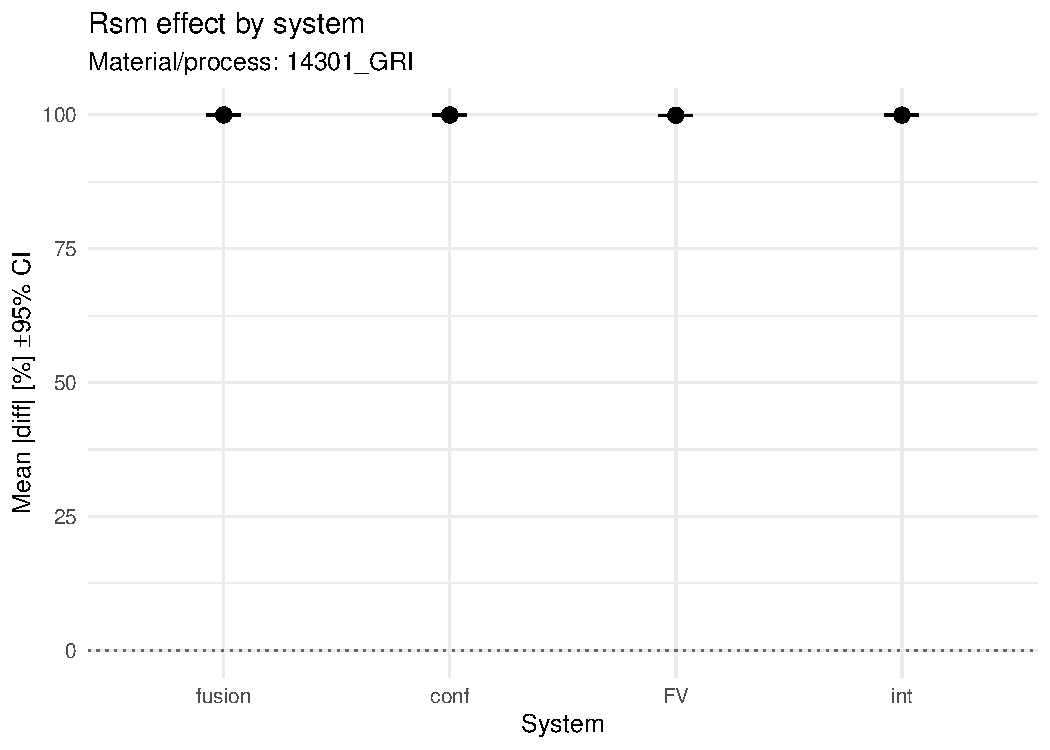
\includegraphics[width=\linewidth]{plots/rsm_abs_14301_gri_effects_by_system.pdf}
\end{minipage}
\begin{minipage}[t]{0.32\textwidth}\centering
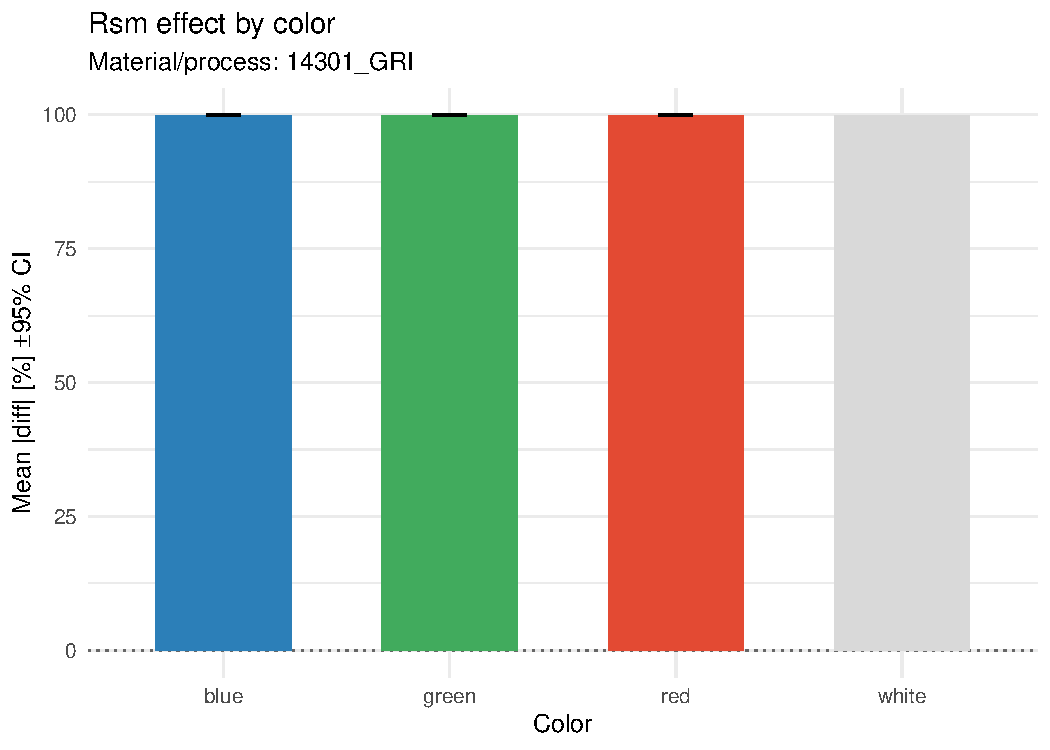
\includegraphics[width=\linewidth]{plots/rsm_abs_14301_gri_effects_by_color.pdf}
\end{minipage}
\caption{RSM — 14301\_gri — porównanie i efekty (|diff| \%)}
\end{figure}

\begin{figure}[H]\centering
\begin{minipage}[t]{0.32\textwidth}\centering
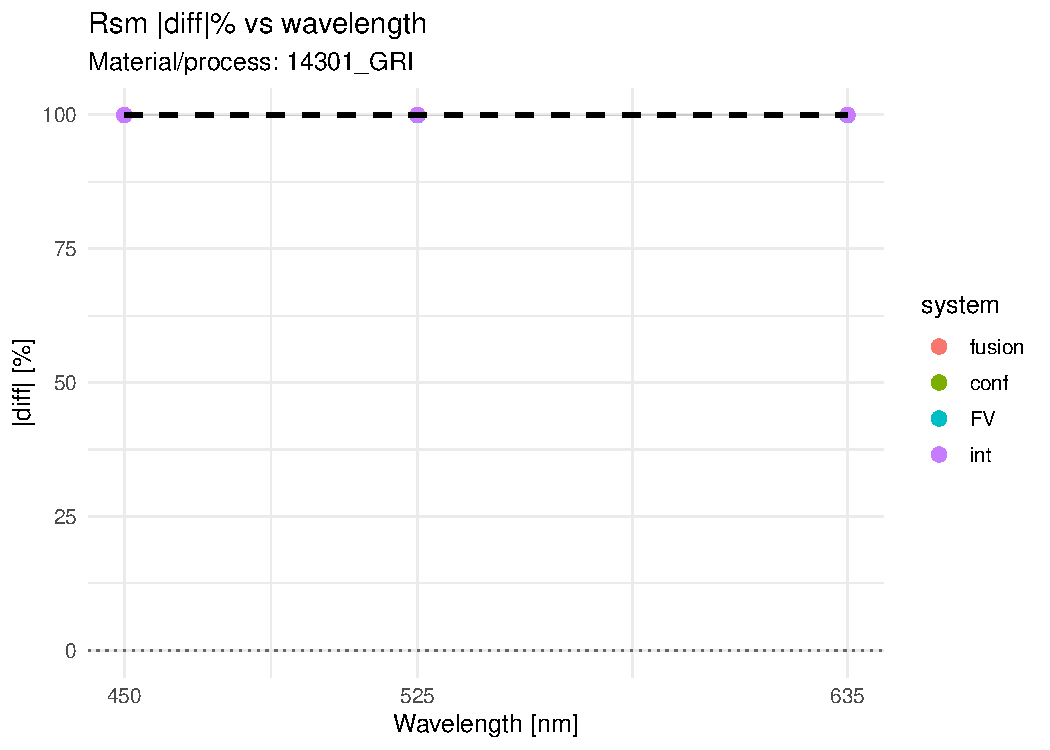
\includegraphics[width=\linewidth]{plots/rsm_abs_14301_gri_diff_vs_wavelength.pdf}
\end{minipage}
\begin{minipage}[t]{0.32\textwidth}\centering
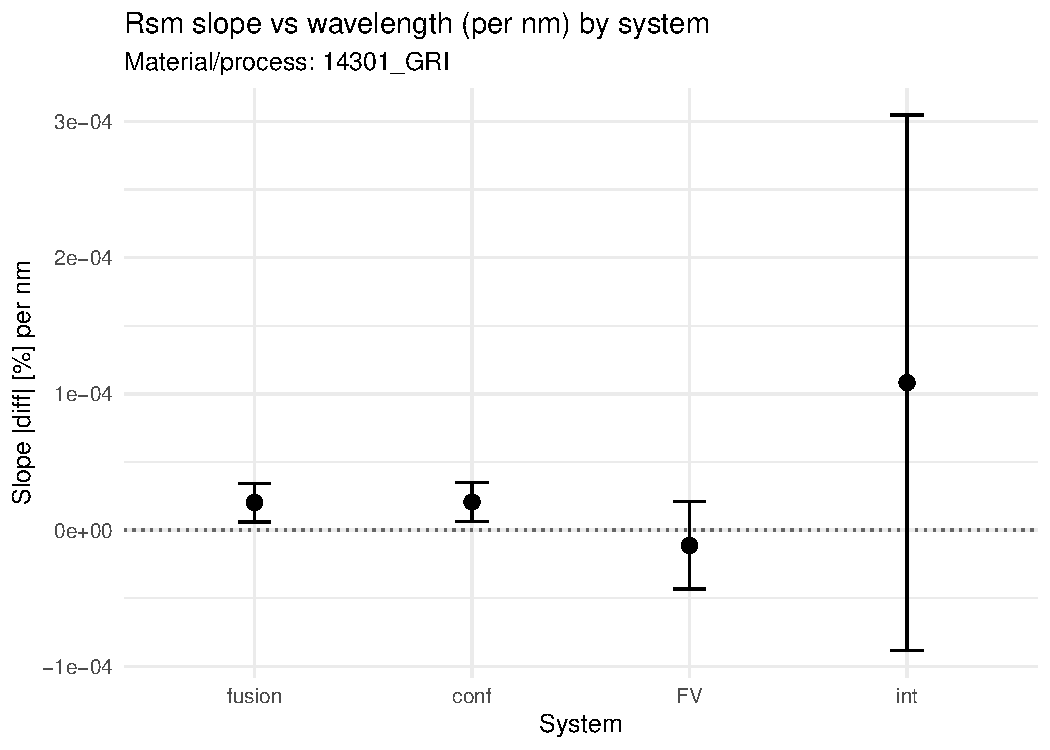
\includegraphics[width=\linewidth]{plots/rsm_abs_14301_gri_slope_by_system_vs_nm.pdf}
\end{minipage}
\begin{minipage}[t]{0.32\textwidth}\centering
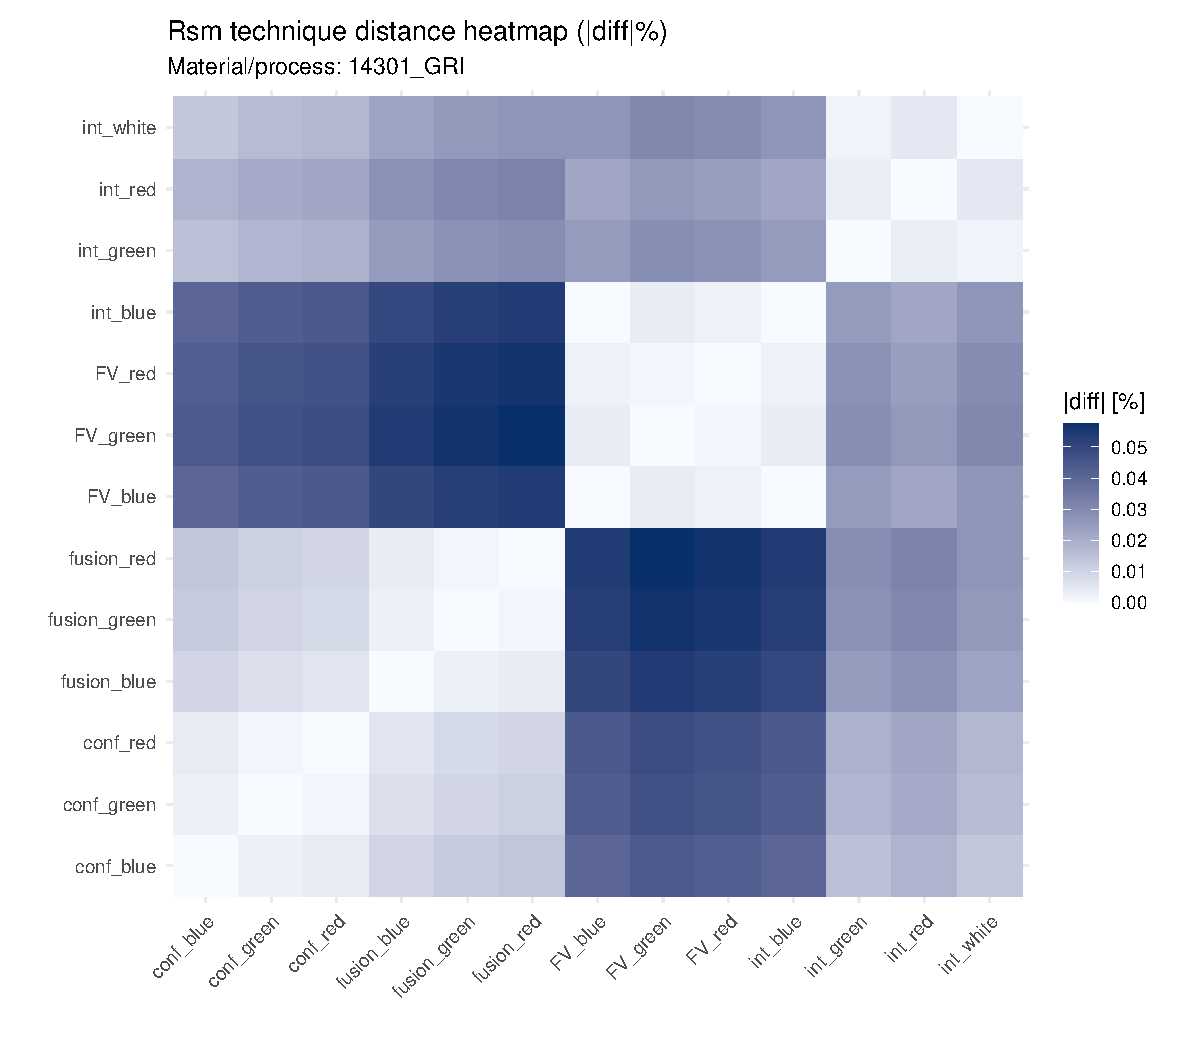
\includegraphics[width=\linewidth]{plots/rsm_abs_14301_gri_tech_distance_heatmap.pdf}
\end{minipage}
\caption{RSM — 14301\_gri — wavelength, nachylenia, odległości technik}
\end{figure}

\begin{figure}[H]\centering
\begin{minipage}[t]{0.32\textwidth}\centering
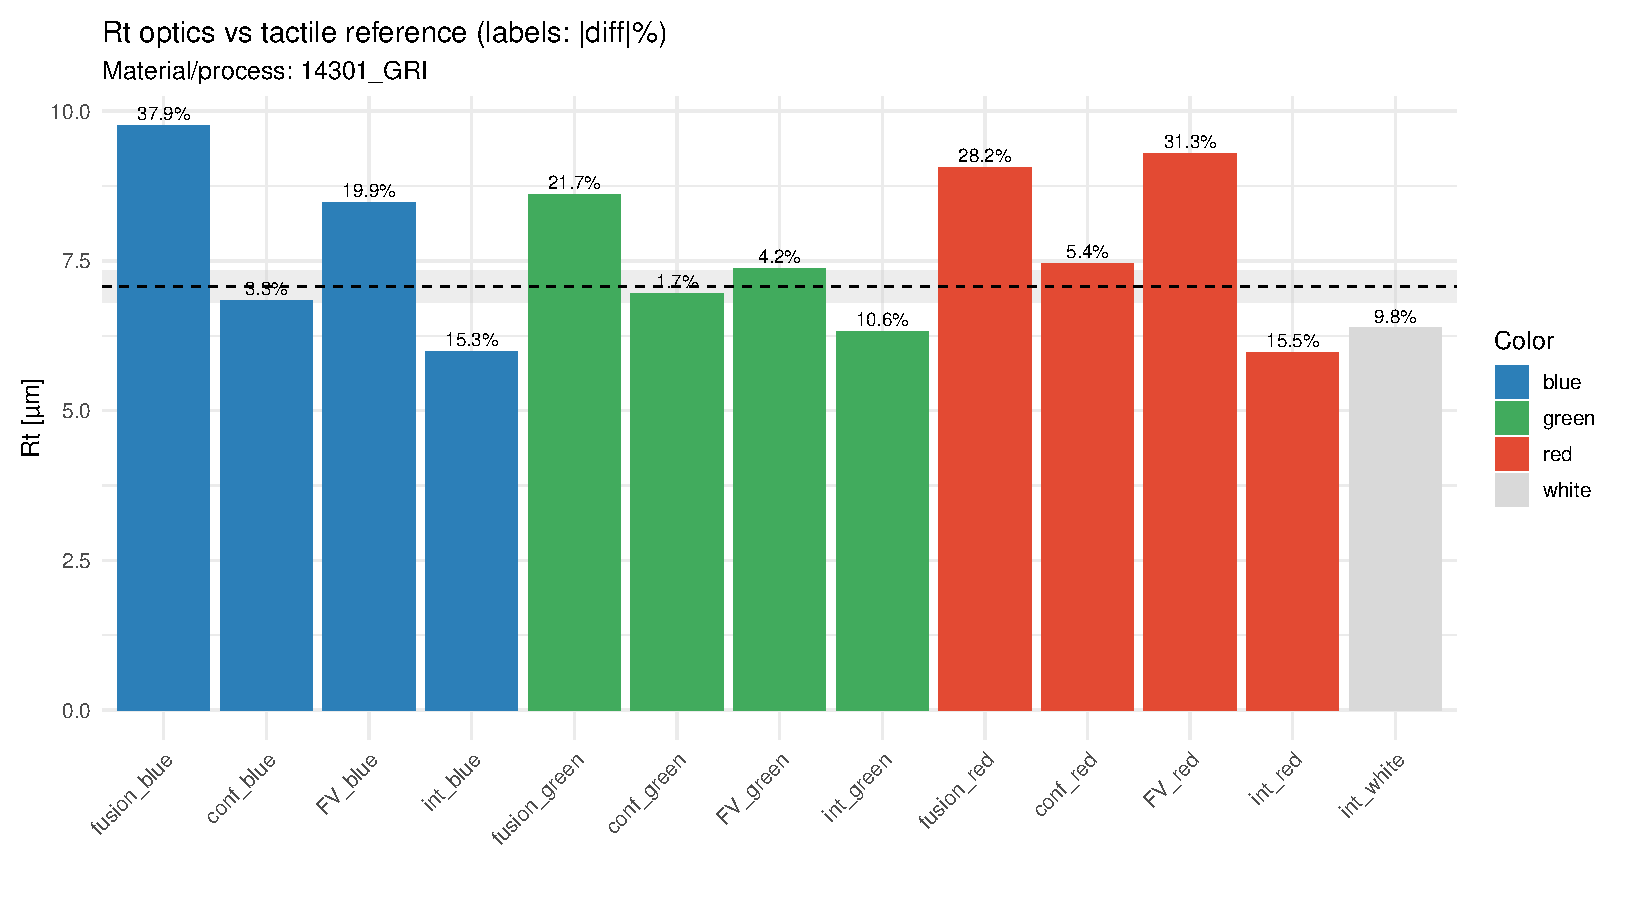
\includegraphics[width=\linewidth]{plots/rt_abs_14301_gri_optics_vs_tactile.pdf}
\end{minipage}
\begin{minipage}[t]{0.32\textwidth}\centering
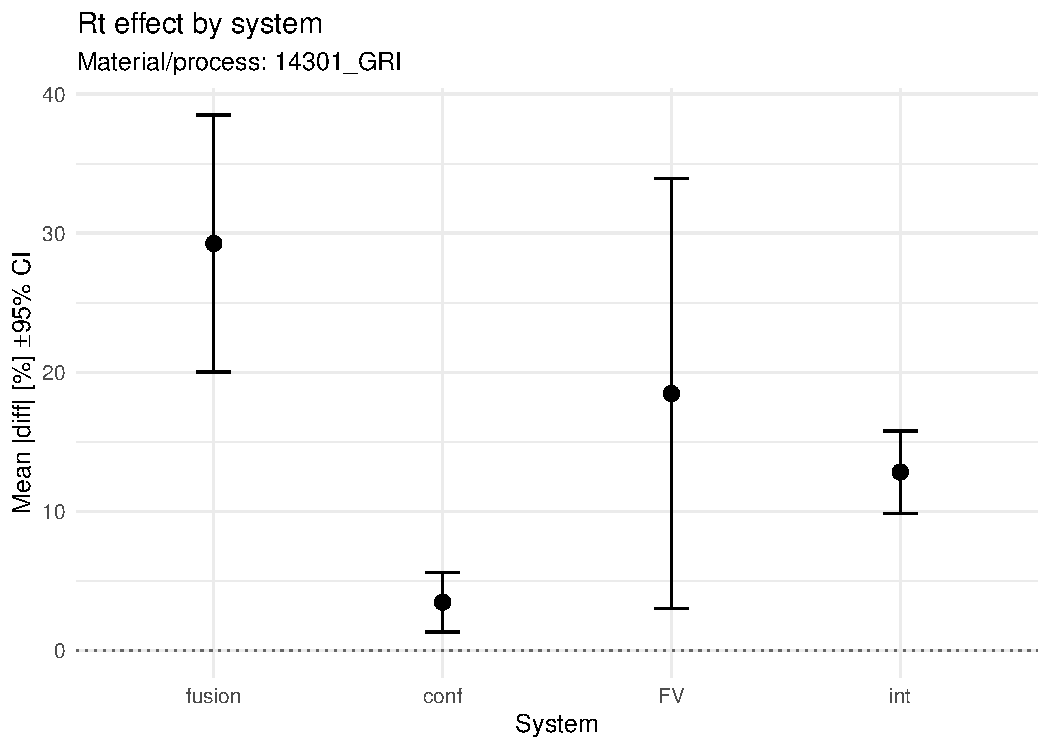
\includegraphics[width=\linewidth]{plots/rt_abs_14301_gri_effects_by_system.pdf}
\end{minipage}
\begin{minipage}[t]{0.32\textwidth}\centering
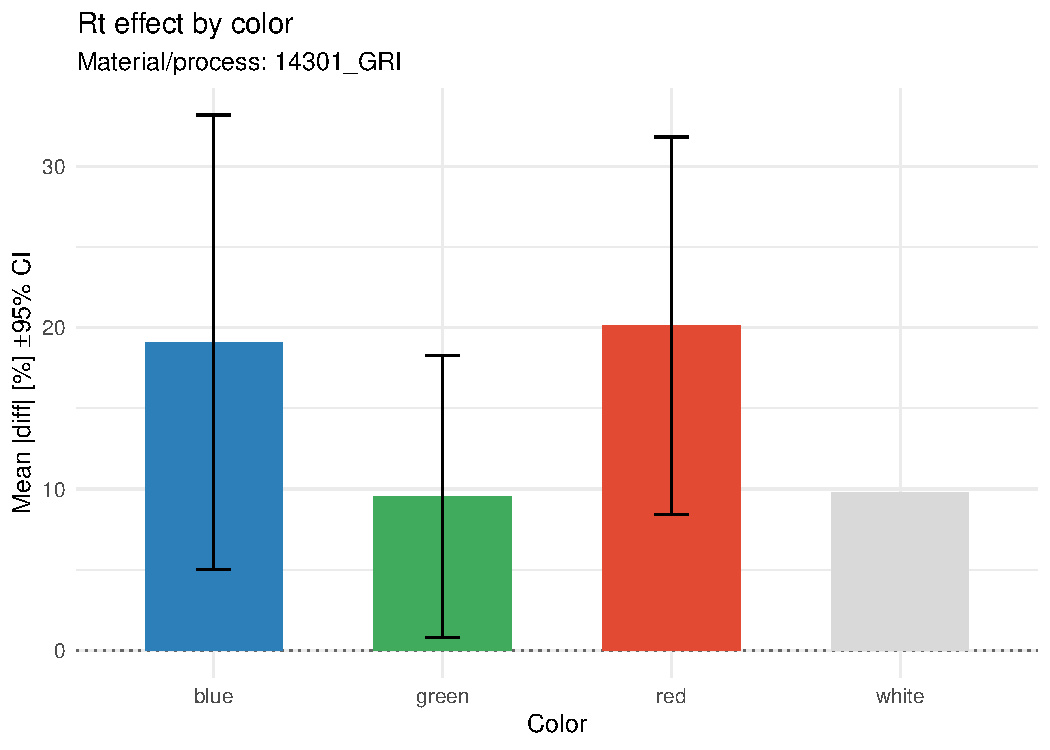
\includegraphics[width=\linewidth]{plots/rt_abs_14301_gri_effects_by_color.pdf}
\end{minipage}
\caption{RT — 14301\_gri — porównanie i efekty (|diff| \%)}
\end{figure}

\begin{figure}[H]\centering
\begin{minipage}[t]{0.32\textwidth}\centering
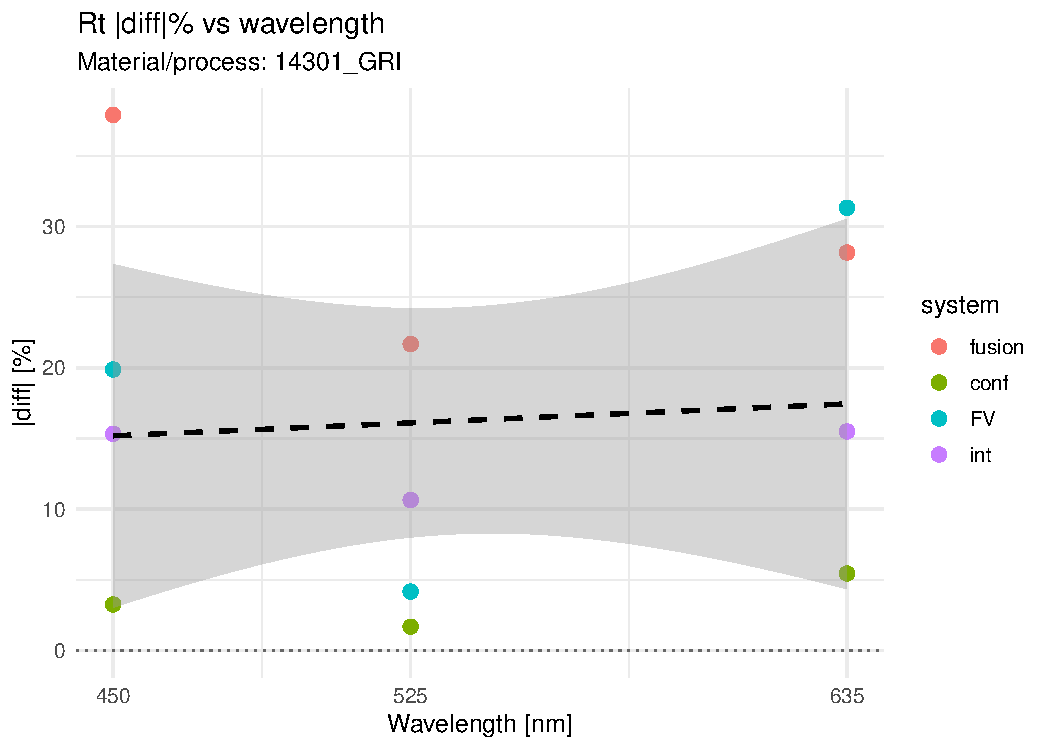
\includegraphics[width=\linewidth]{plots/rt_abs_14301_gri_diff_vs_wavelength.pdf}
\end{minipage}
\begin{minipage}[t]{0.32\textwidth}\centering
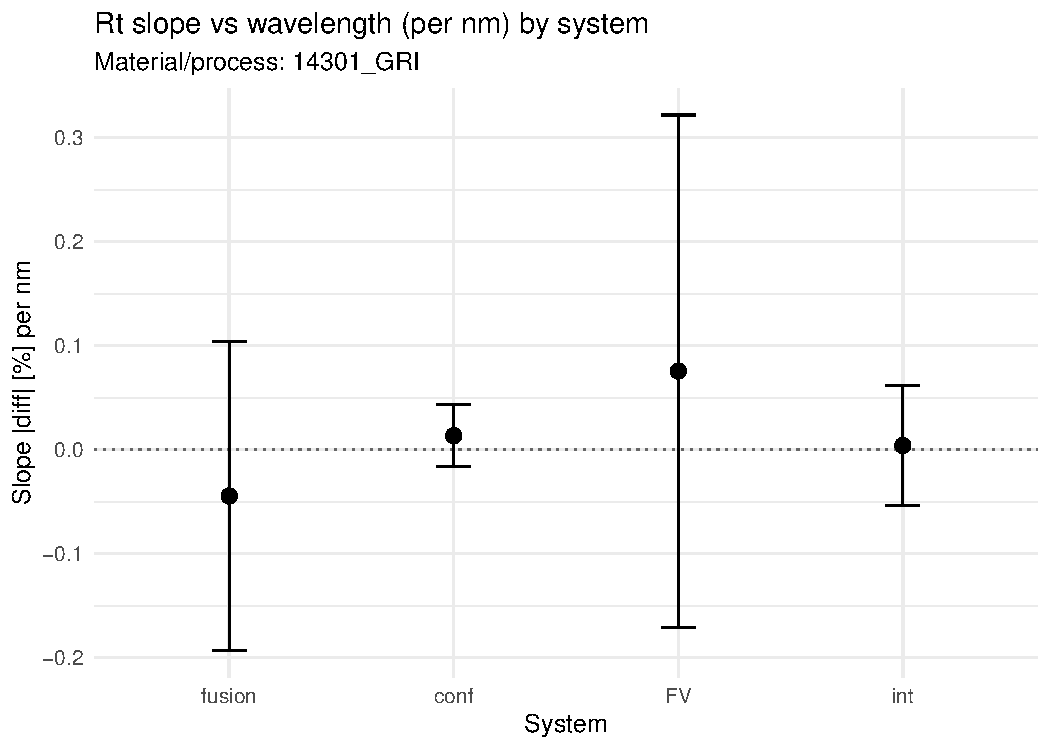
\includegraphics[width=\linewidth]{plots/rt_abs_14301_gri_slope_by_system_vs_nm.pdf}
\end{minipage}
\begin{minipage}[t]{0.32\textwidth}\centering
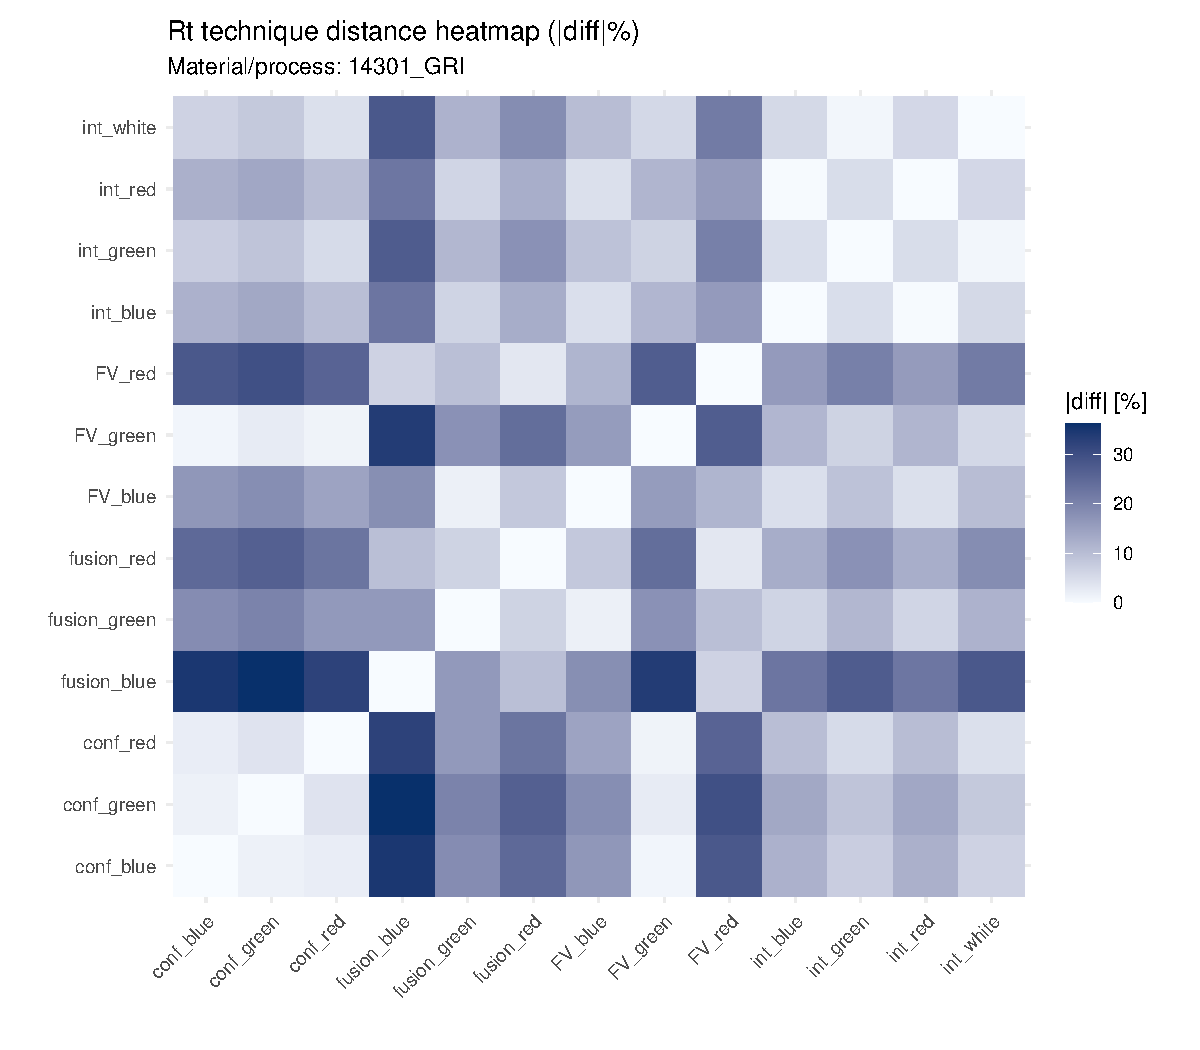
\includegraphics[width=\linewidth]{plots/rt_abs_14301_gri_tech_distance_heatmap.pdf}
\end{minipage}
\caption{RT — 14301\_gri — wavelength, nachylenia, odległości technik}
\end{figure}

\begin{figure}[H]\centering
\begin{minipage}[t]{0.32\textwidth}\centering
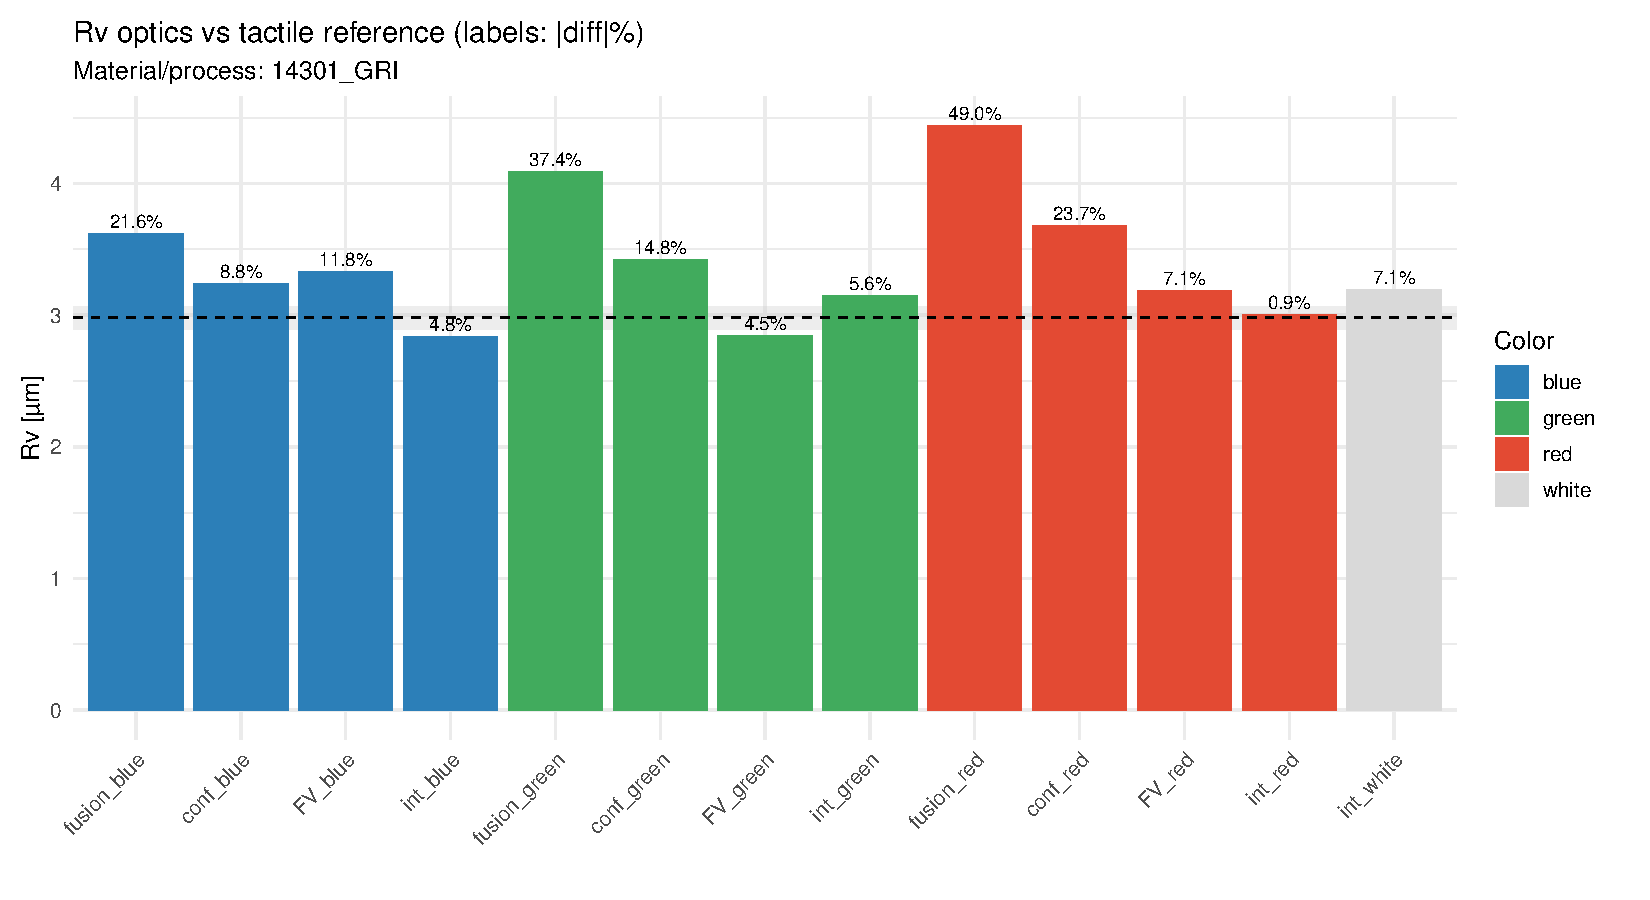
\includegraphics[width=\linewidth]{plots/rv_abs_14301_gri_optics_vs_tactile.pdf}
\end{minipage}
\begin{minipage}[t]{0.32\textwidth}\centering
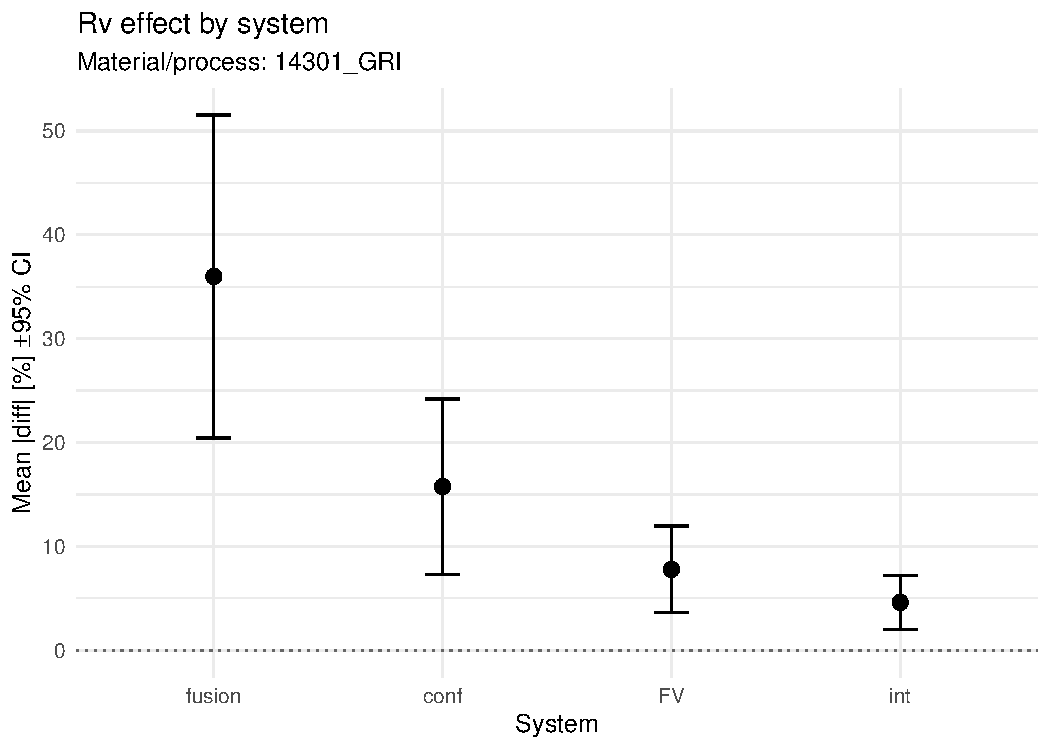
\includegraphics[width=\linewidth]{plots/rv_abs_14301_gri_effects_by_system.pdf}
\end{minipage}
\begin{minipage}[t]{0.32\textwidth}\centering
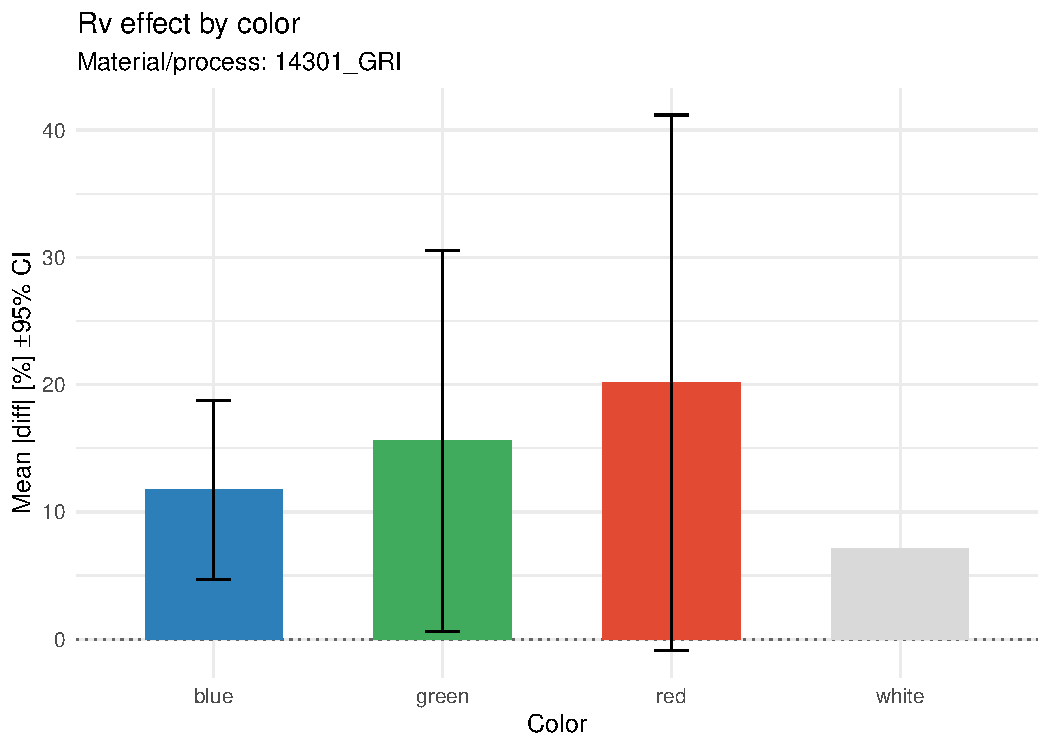
\includegraphics[width=\linewidth]{plots/rv_abs_14301_gri_effects_by_color.pdf}
\end{minipage}
\caption{RV — 14301\_gri — porównanie i efekty (|diff| \%)}
\end{figure}

\begin{figure}[H]\centering
\begin{minipage}[t]{0.32\textwidth}\centering
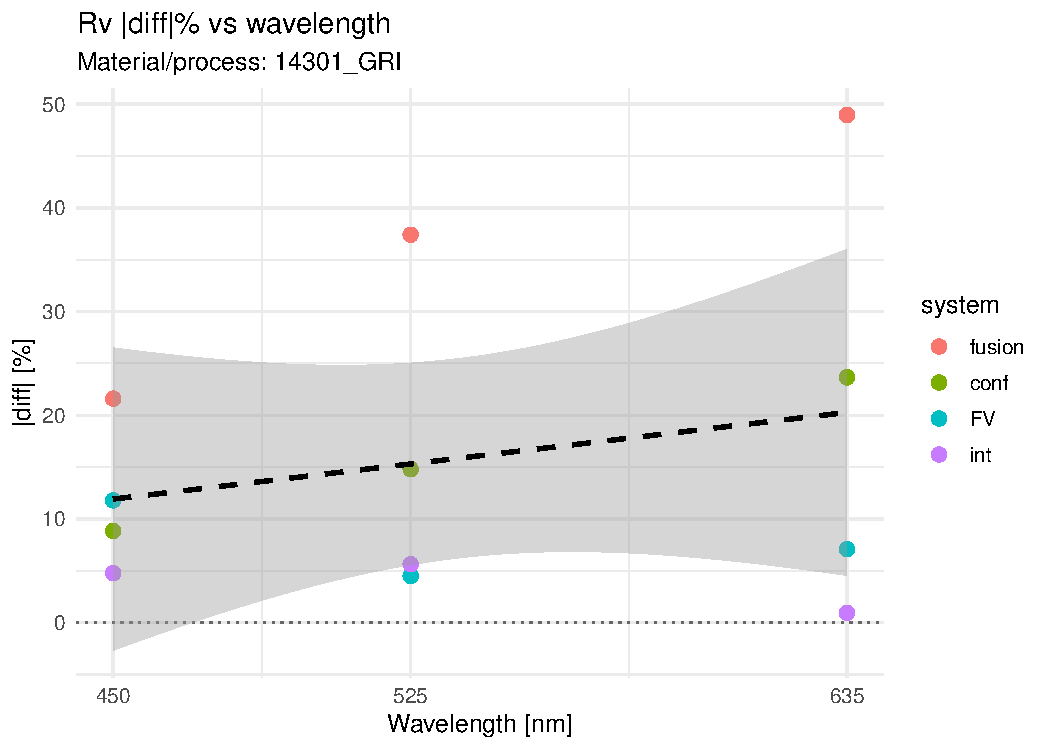
\includegraphics[width=\linewidth]{plots/rv_abs_14301_gri_diff_vs_wavelength.pdf}
\end{minipage}
\begin{minipage}[t]{0.32\textwidth}\centering
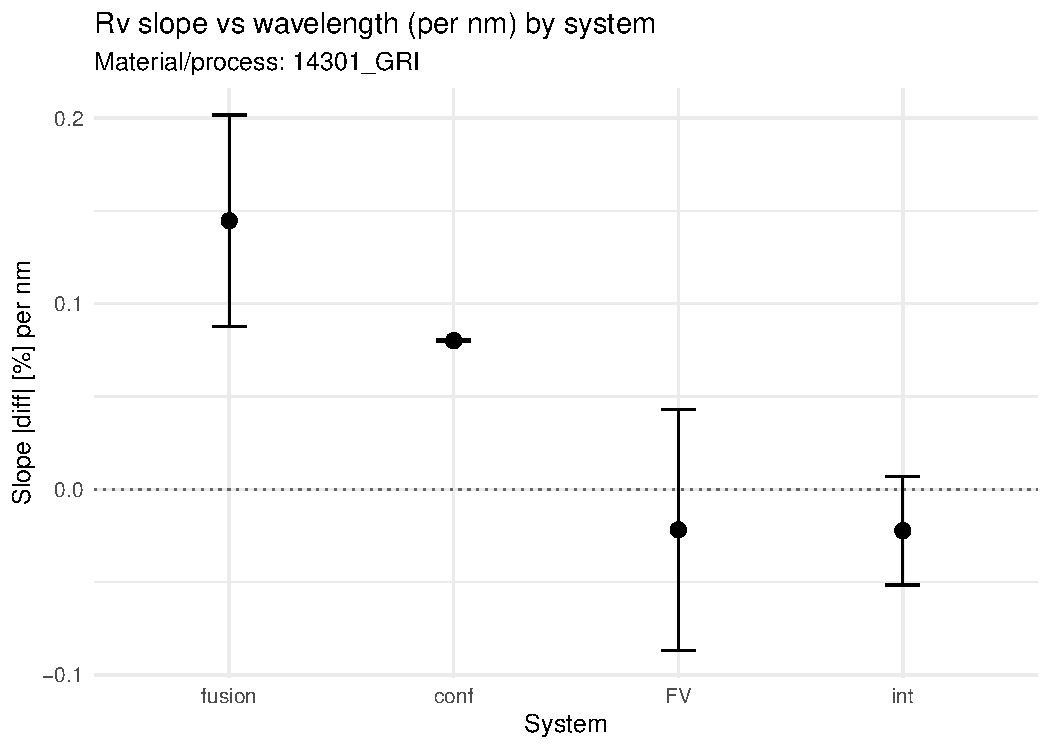
\includegraphics[width=\linewidth]{plots/rv_abs_14301_gri_slope_by_system_vs_nm.pdf}
\end{minipage}
\begin{minipage}[t]{0.32\textwidth}\centering
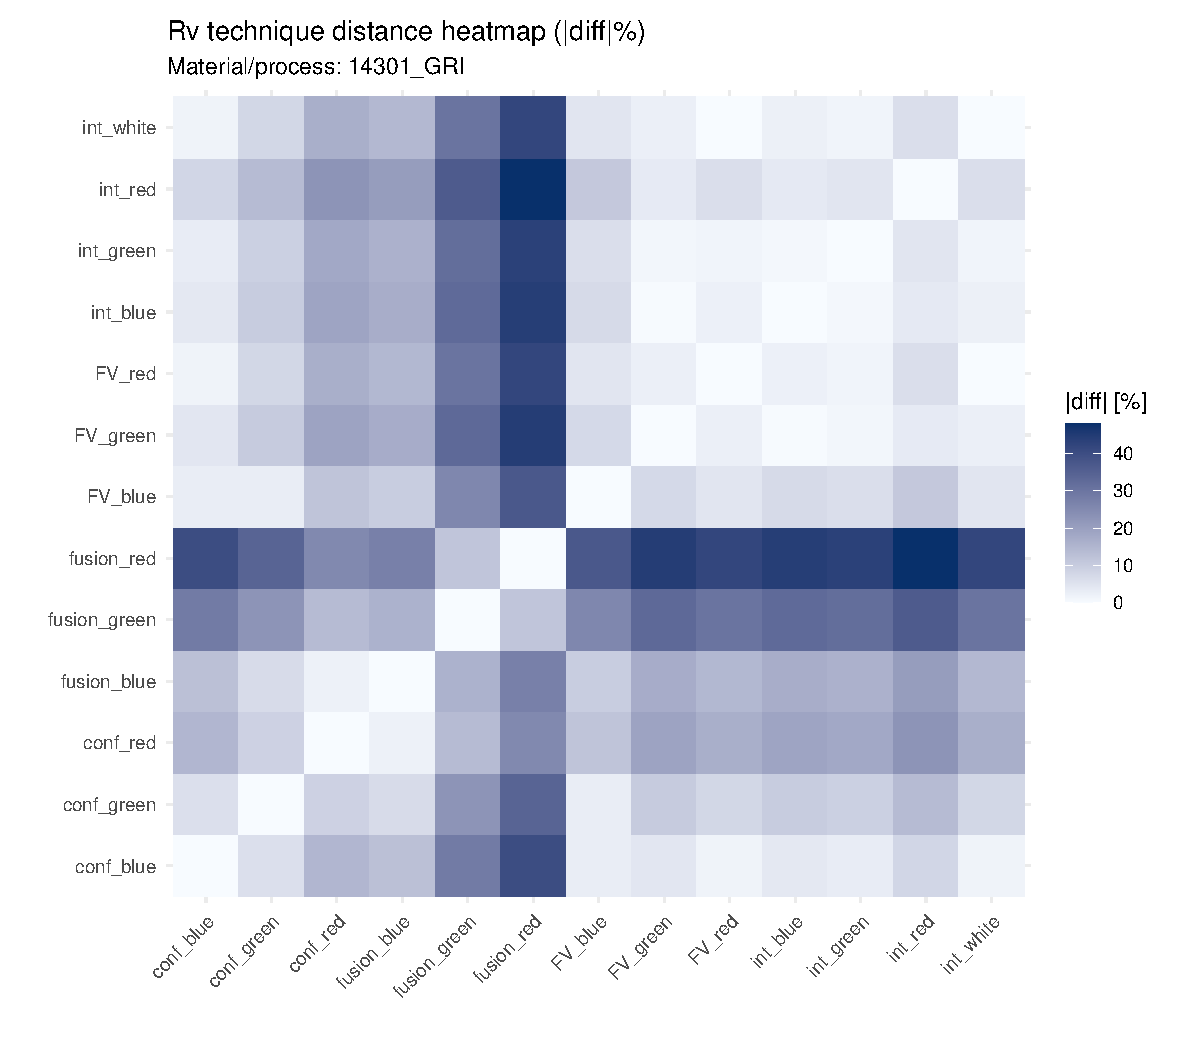
\includegraphics[width=\linewidth]{plots/rv_abs_14301_gri_tech_distance_heatmap.pdf}
\end{minipage}
\caption{RV — 14301\_gri — wavelength, nachylenia, odległości technik}
\end{figure}

\begin{figure}[H]\centering
\begin{minipage}[t]{0.32\textwidth}\centering
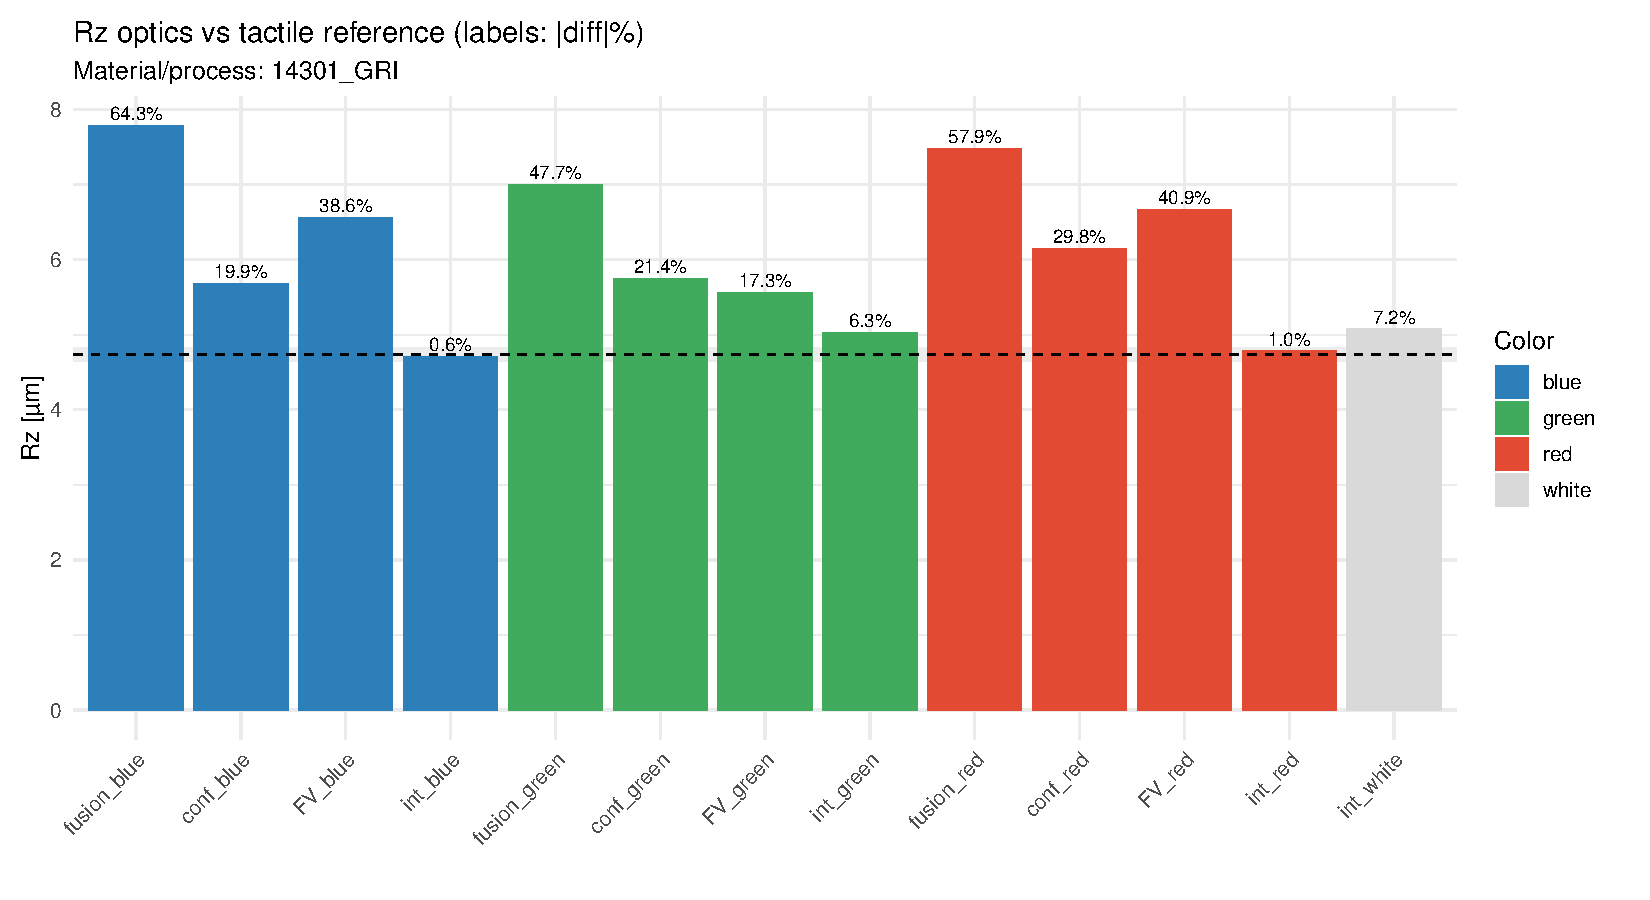
\includegraphics[width=\linewidth]{plots/rz_abs_14301_gri_optics_vs_tactile.pdf}
\end{minipage}
\begin{minipage}[t]{0.32\textwidth}\centering
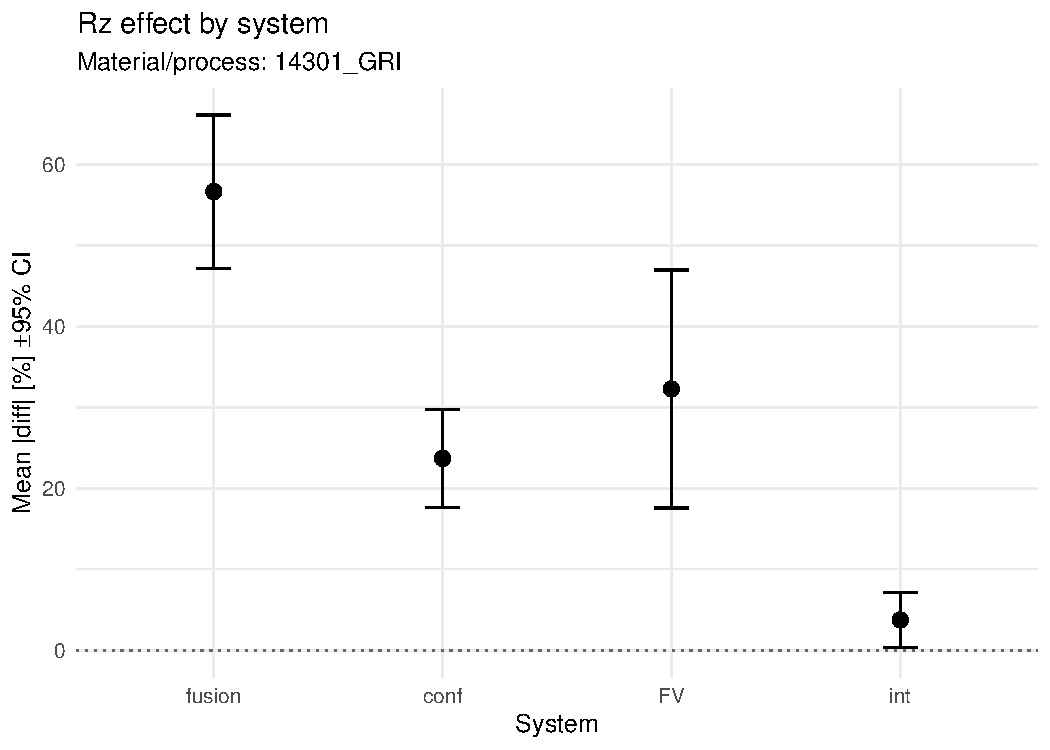
\includegraphics[width=\linewidth]{plots/rz_abs_14301_gri_effects_by_system.pdf}
\end{minipage}
\begin{minipage}[t]{0.32\textwidth}\centering
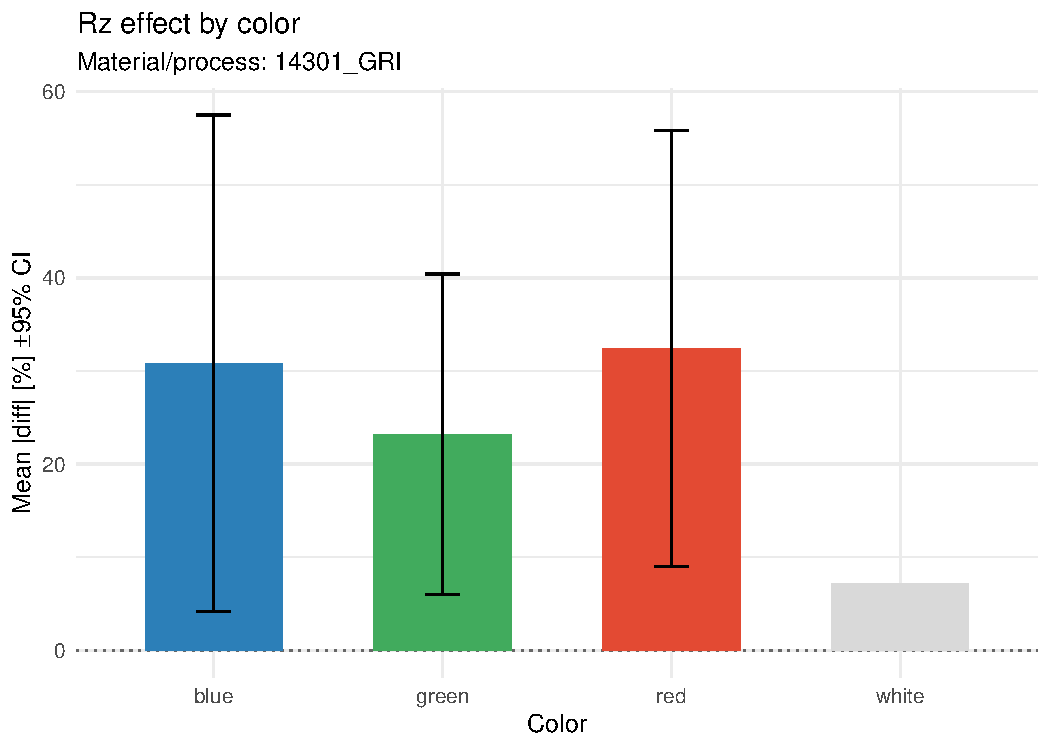
\includegraphics[width=\linewidth]{plots/rz_abs_14301_gri_effects_by_color.pdf}
\end{minipage}
\caption{RZ — 14301\_gri — porównanie i efekty (|diff| \%)}
\end{figure}

\begin{figure}[H]\centering
\begin{minipage}[t]{0.32\textwidth}\centering
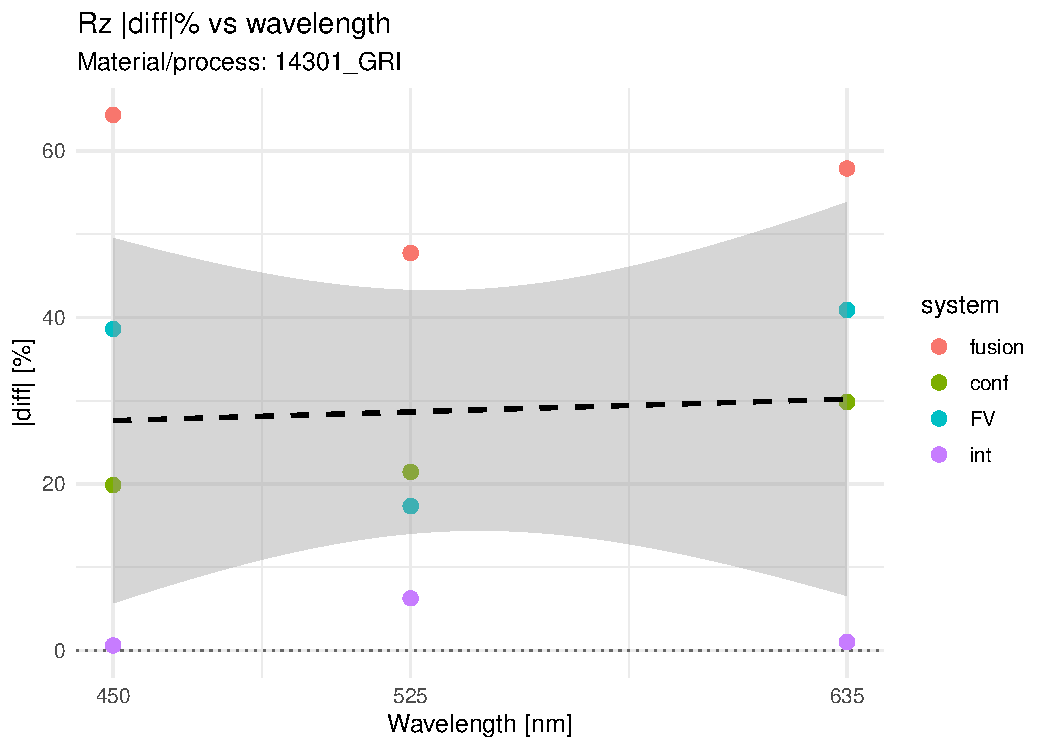
\includegraphics[width=\linewidth]{plots/rz_abs_14301_gri_diff_vs_wavelength.pdf}
\end{minipage}
\begin{minipage}[t]{0.32\textwidth}\centering
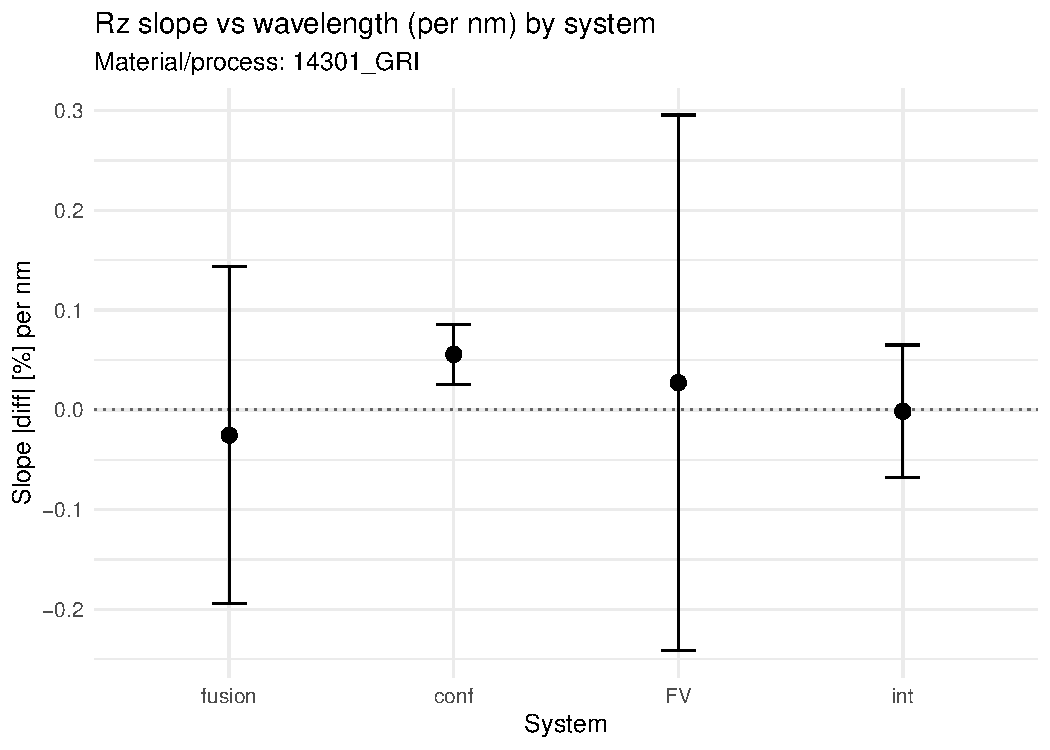
\includegraphics[width=\linewidth]{plots/rz_abs_14301_gri_slope_by_system_vs_nm.pdf}
\end{minipage}
\begin{minipage}[t]{0.32\textwidth}\centering
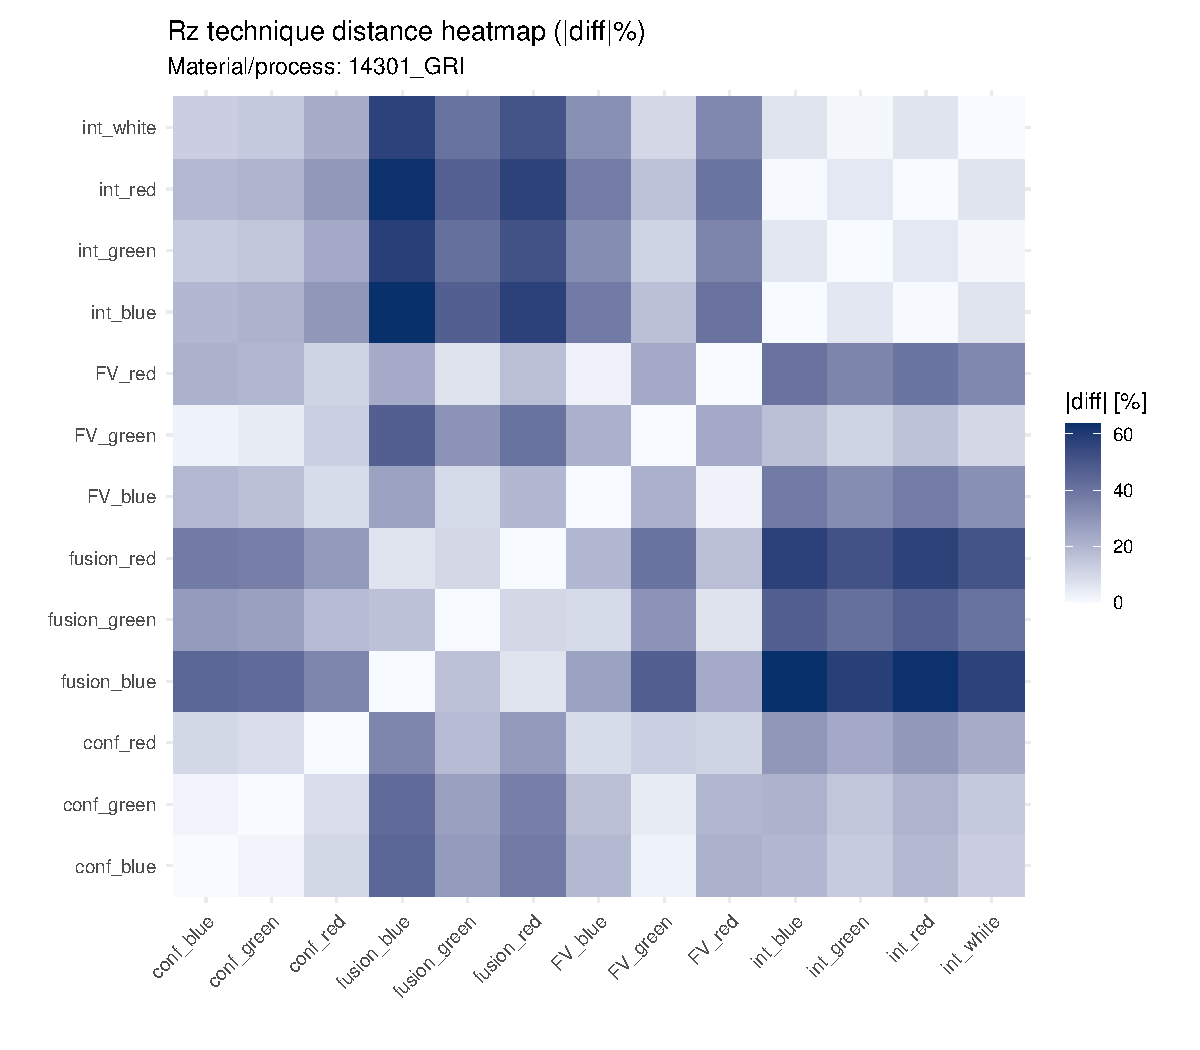
\includegraphics[width=\linewidth]{plots/rz_abs_14301_gri_tech_distance_heatmap.pdf}
\end{minipage}
\caption{RZ — 14301\_gri — wavelength, nachylenia, odległości technik}
\end{figure}

\begin{figure}[H]\centering
\begin{minipage}[t]{0.32\textwidth}\centering
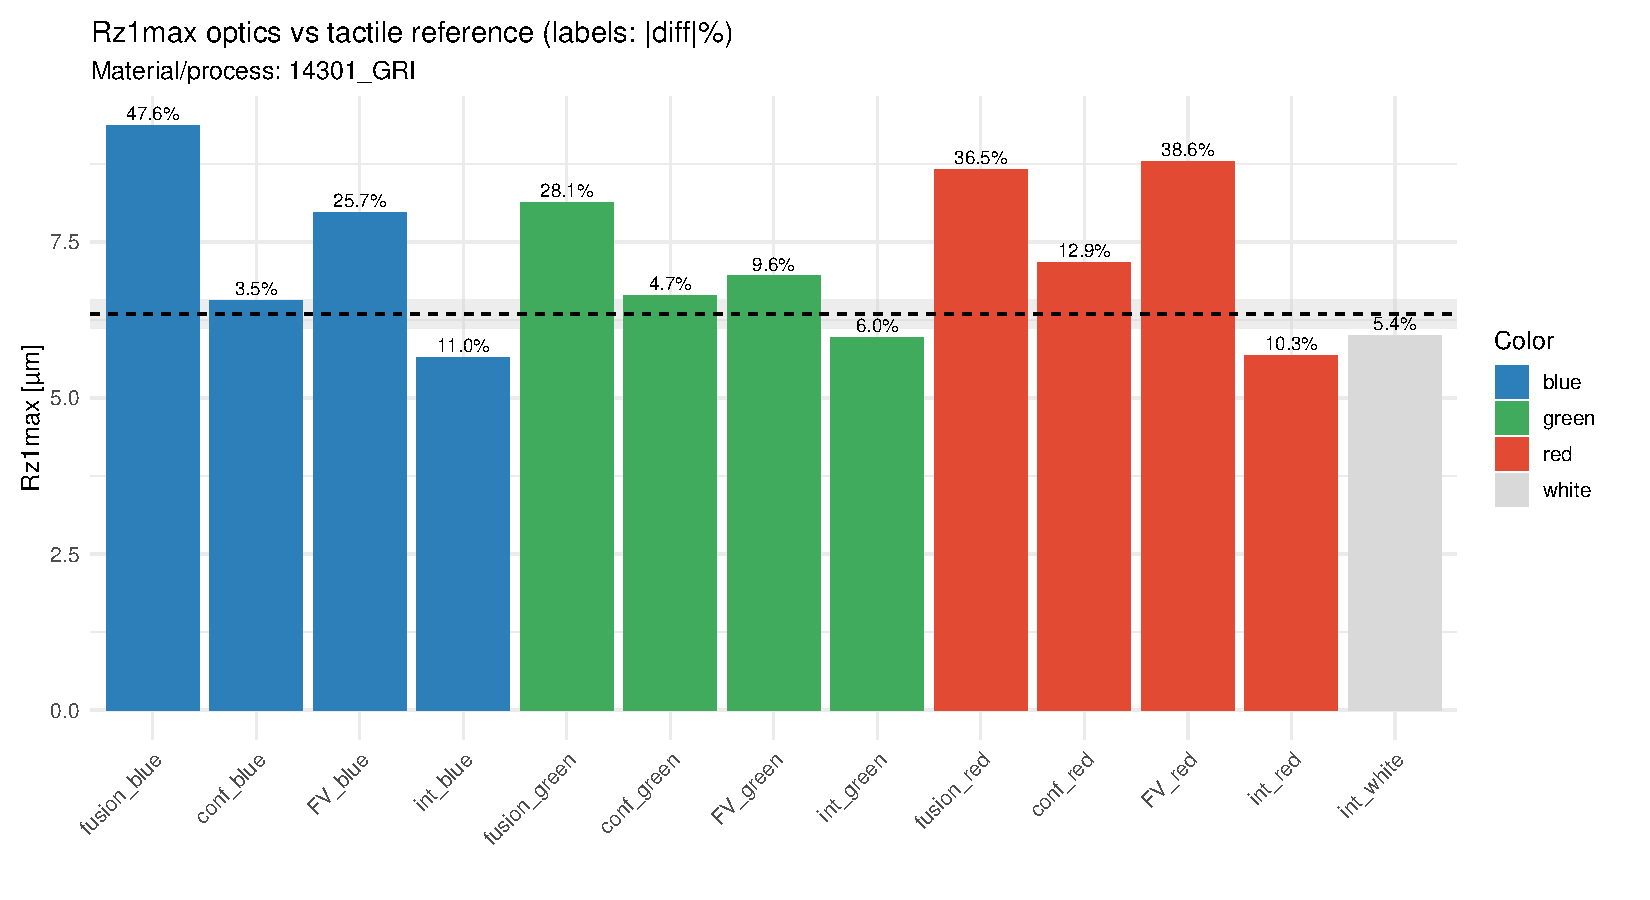
\includegraphics[width=\linewidth]{plots/rz1max_abs_14301_gri_optics_vs_tactile.pdf}
\end{minipage}
\begin{minipage}[t]{0.32\textwidth}\centering
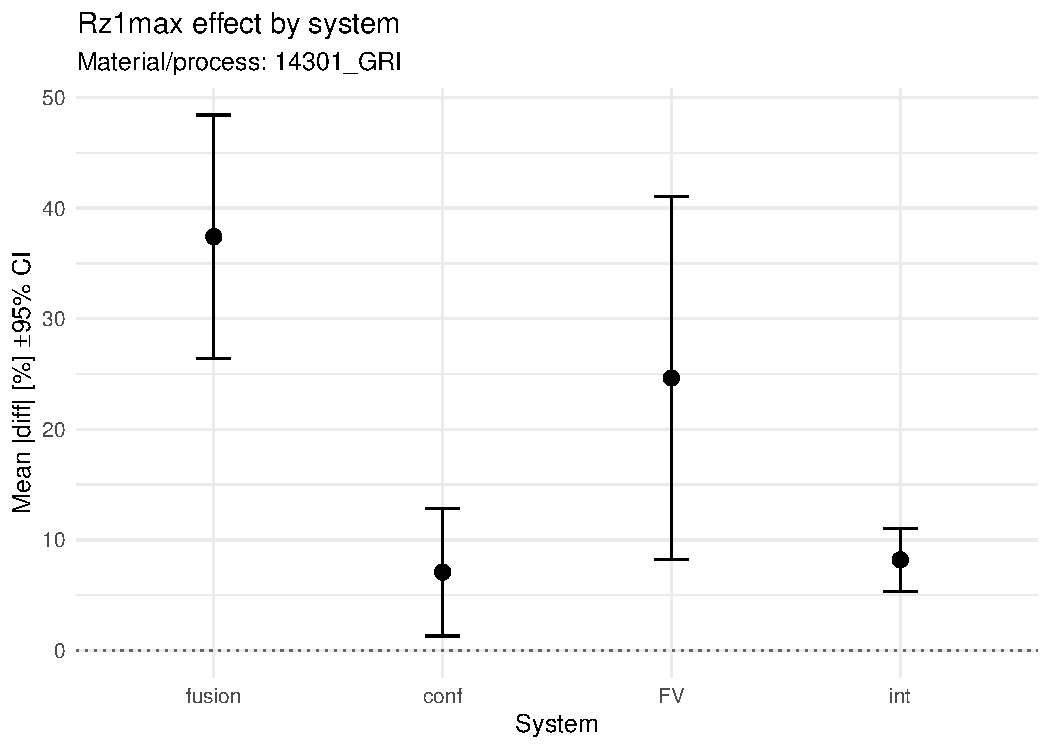
\includegraphics[width=\linewidth]{plots/rz1max_abs_14301_gri_effects_by_system.pdf}
\end{minipage}
\begin{minipage}[t]{0.32\textwidth}\centering
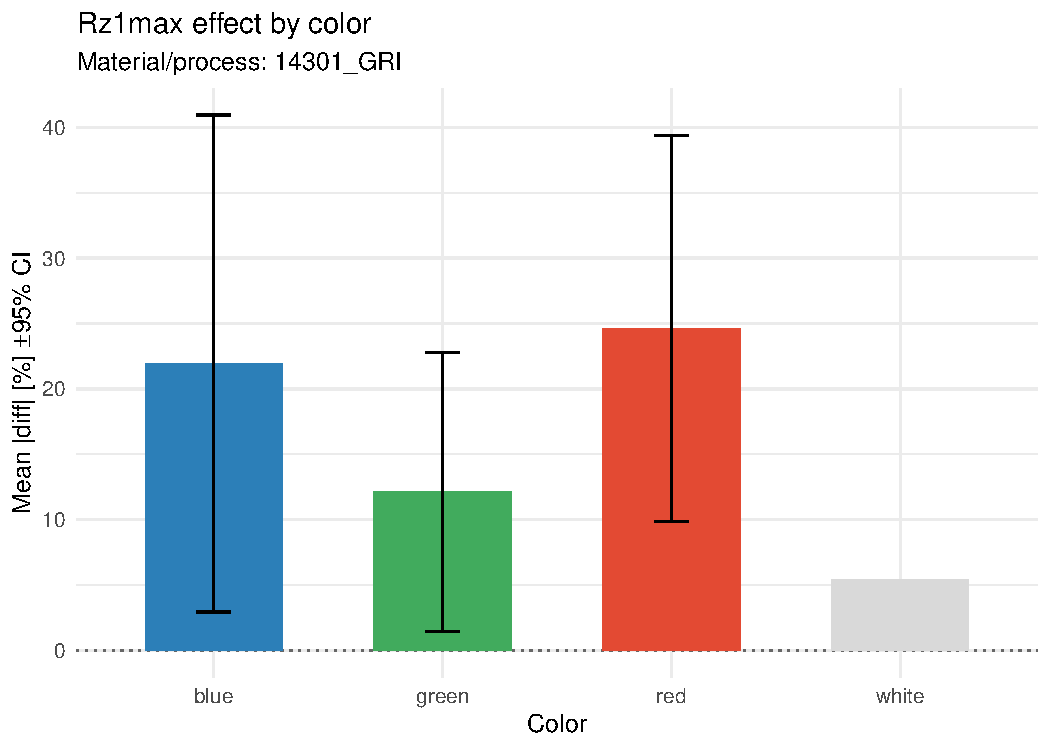
\includegraphics[width=\linewidth]{plots/rz1max_abs_14301_gri_effects_by_color.pdf}
\end{minipage}
\caption{RZ1MAX — 14301\_gri — porównanie i efekty (|diff| \%)}
\end{figure}

\begin{figure}[H]\centering
\begin{minipage}[t]{0.32\textwidth}\centering
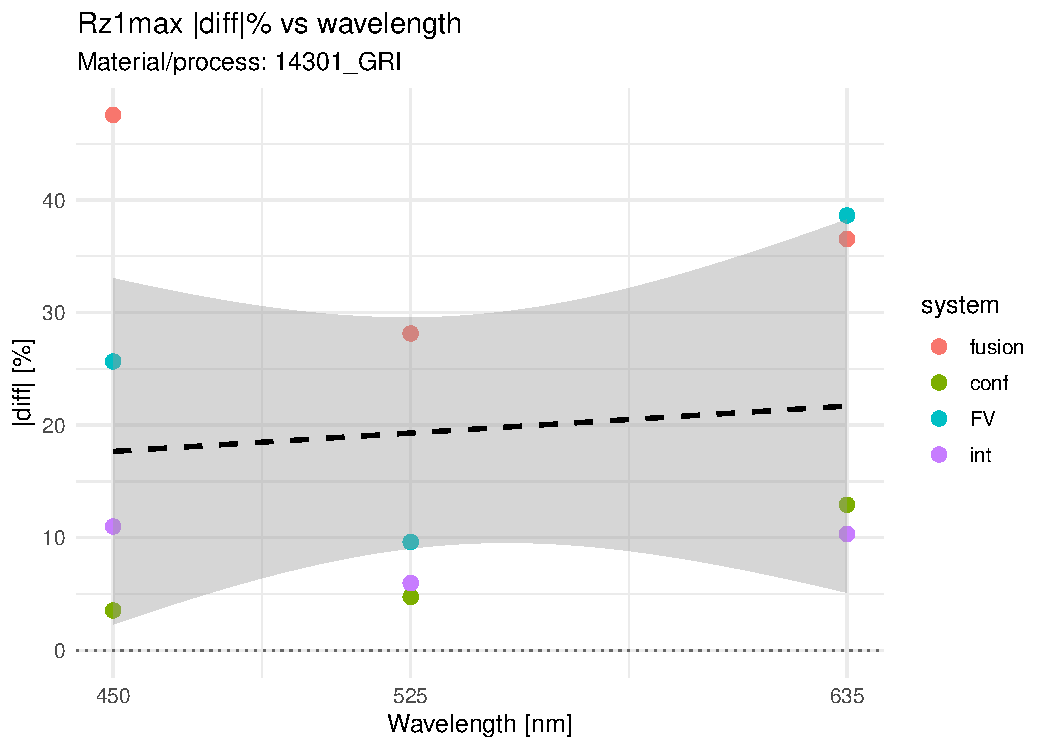
\includegraphics[width=\linewidth]{plots/rz1max_abs_14301_gri_diff_vs_wavelength.pdf}
\end{minipage}
\begin{minipage}[t]{0.32\textwidth}\centering
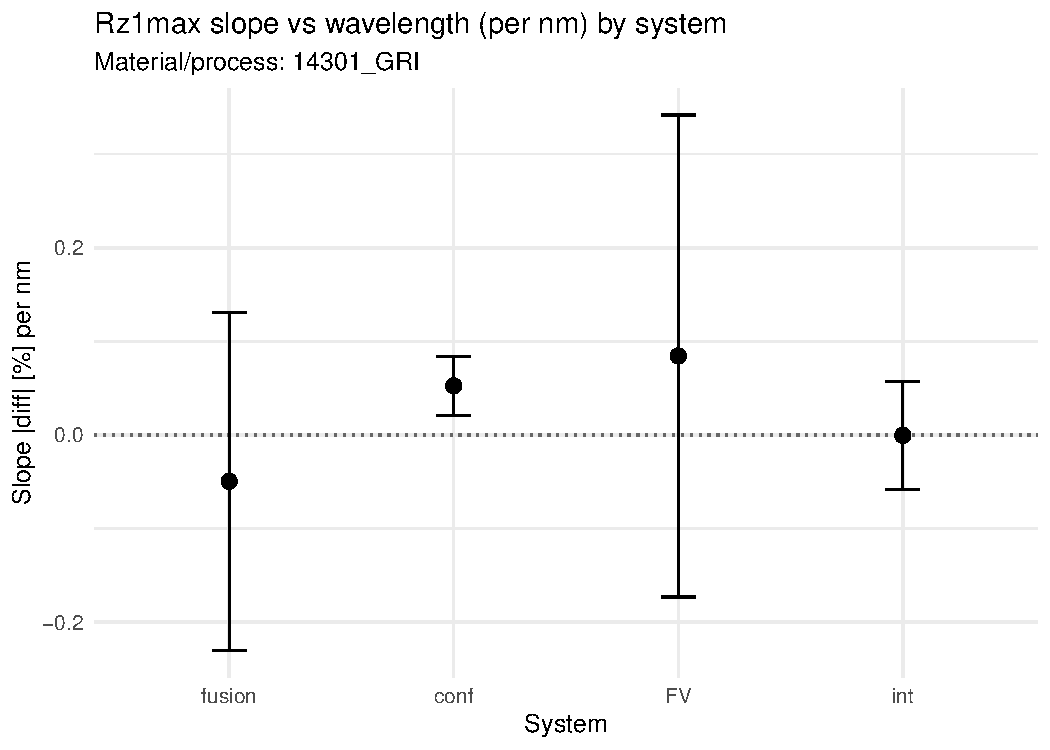
\includegraphics[width=\linewidth]{plots/rz1max_abs_14301_gri_slope_by_system_vs_nm.pdf}
\end{minipage}
\begin{minipage}[t]{0.32\textwidth}\centering
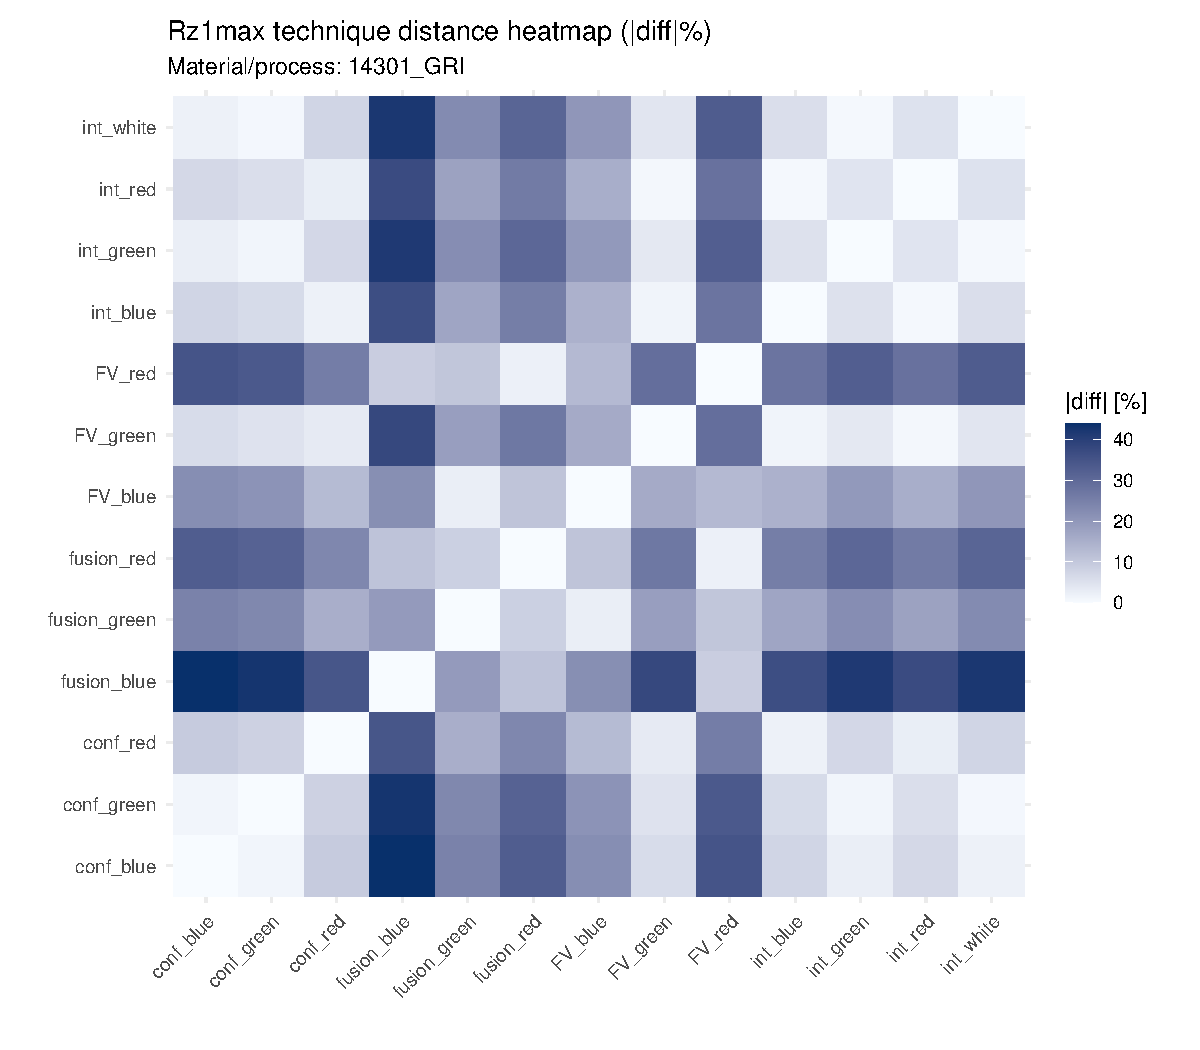
\includegraphics[width=\linewidth]{plots/rz1max_abs_14301_gri_tech_distance_heatmap.pdf}
\end{minipage}
\caption{RZ1MAX — 14301\_gri — wavelength, nachylenia, odległości technik}
\end{figure}

\subsection{Wyniki i wnioski dla materiał/proces: 14301\_gri}

\textbf{RA}. r=0.167, rho=0.148; eta2: system=0.809, color=0.052.
Istotne nachylenia: conf(slope=0.086, p=0.010). Trendy (p\textless0.1):
fusion(slope=0.093, p=0.071). Wniosek: TAK. \textbf{RKU}. r=0.073,
rho=0.089; eta2: system=0.675, color=0.018. Wniosek: NIE. \textbf{RP}.
r=-0.112, rho=-0.059; eta2: system=0.795, color=0.070. Wniosek: NIE.
\textbf{RQ}. r=0.156, rho=0.148; eta2: system=0.821, color=0.055.
Istotne nachylenia: conf(slope=0.076, p=0.025). Wniosek: TAK.
\textbf{RSK}. r=-0.189, rho=-0.236; eta2: system=0.823, color=0.076.
Wniosek: NIE. \textbf{RSM}. r=0.118, rho=0.118; eta2: system=0.917,
color=0.037. Wniosek: NIE. \textbf{RT}. r=0.082, rho=0.118; eta2:
system=0.662, color=0.178. Wniosek: NIE. \textbf{RV}. r=0.244,
rho=0.089; eta2: system=0.781, color=0.061. Istotne nachylenia:
conf(slope=0.080, p=0.002). Wniosek: TAK. \textbf{RZ}. r=0.052,
rho=0.089; eta2: system=0.896, color=0.038. Wniosek: NIE.
\textbf{RZ1MAX}. r=0.114, rho=0.177; eta2: system=0.744, color=0.132.
Wniosek: NIE.

\paragraph{Podsumowanie (opisowe) dla tego materiału/procesu}
\begin{itemize}
\item W ujęciu ANOVA: częściej dominuje system (eta²).
\item Najczęściej preferowany system (min średni |diff|): int.
\item Najczęściej preferowana barwa (min średni |diff|): white.
\item Zależność od wavelength wykryta (p<0.05) dla parametrów: RA, RQ, RV; dotyczy systemów: conf.
\end{itemize}
\paragraph{Rekomendacje dla tego materiału}
\begin{itemize}
\item RA: preferowany system (min średni |diff|): int; preferowana barwa (min średni |diff|): white; dominuje system; zależność od wavelength: TAK (p<0.05) — conf: rośnie.
\item RKU: preferowany system (min średni |diff|): int; preferowana barwa (min średni |diff|): white; dominuje system; zależność od wavelength: NIE (brak wykrytego trendu per system).
\item RP: preferowany system (min średni |diff|): int; preferowana barwa (min średni |diff|): white; dominuje system; zależność od wavelength: NIE (brak wykrytego trendu per system).
\item RQ: preferowany system (min średni |diff|): int; preferowana barwa (min średni |diff|): white; dominuje system; zależność od wavelength: TAK (p<0.05) — conf: rośnie.
\item RSK: preferowany system (min średni |diff|): int; preferowana barwa (min średni |diff|): white; dominuje system; zależność od wavelength: NIE (brak wykrytego trendu per system).
\item RSM: preferowany system (min średni |diff|): FV; preferowana barwa (min średni |diff|): blue; dominuje system; zależność od wavelength: NIE (brak wykrytego trendu per system).
\item RT: preferowany system (min średni |diff|): conf; preferowana barwa (min średni |diff|): green; dominuje system; zależność od wavelength: NIE (brak wykrytego trendu per system).
\item RV: preferowany system (min średni |diff|): int; preferowana barwa (min średni |diff|): white; dominuje system; zależność od wavelength: TAK (p<0.05) — conf: rośnie.
\item RZ: preferowany system (min średni |diff|): int; preferowana barwa (min średni |diff|): white; dominuje system; zależność od wavelength: NIE (brak wykrytego trendu per system).
\item RZ1MAX: preferowany system (min średni |diff|): conf; preferowana barwa (min średni |diff|): white; dominuje system; zależność od wavelength: NIE (brak wykrytego trendu per system).
\end{itemize}
\subsubsection{Materiał/proces: 14301\_hon}
\begin{figure}[H]\centering
\begin{minipage}[t]{0.32\textwidth}\centering
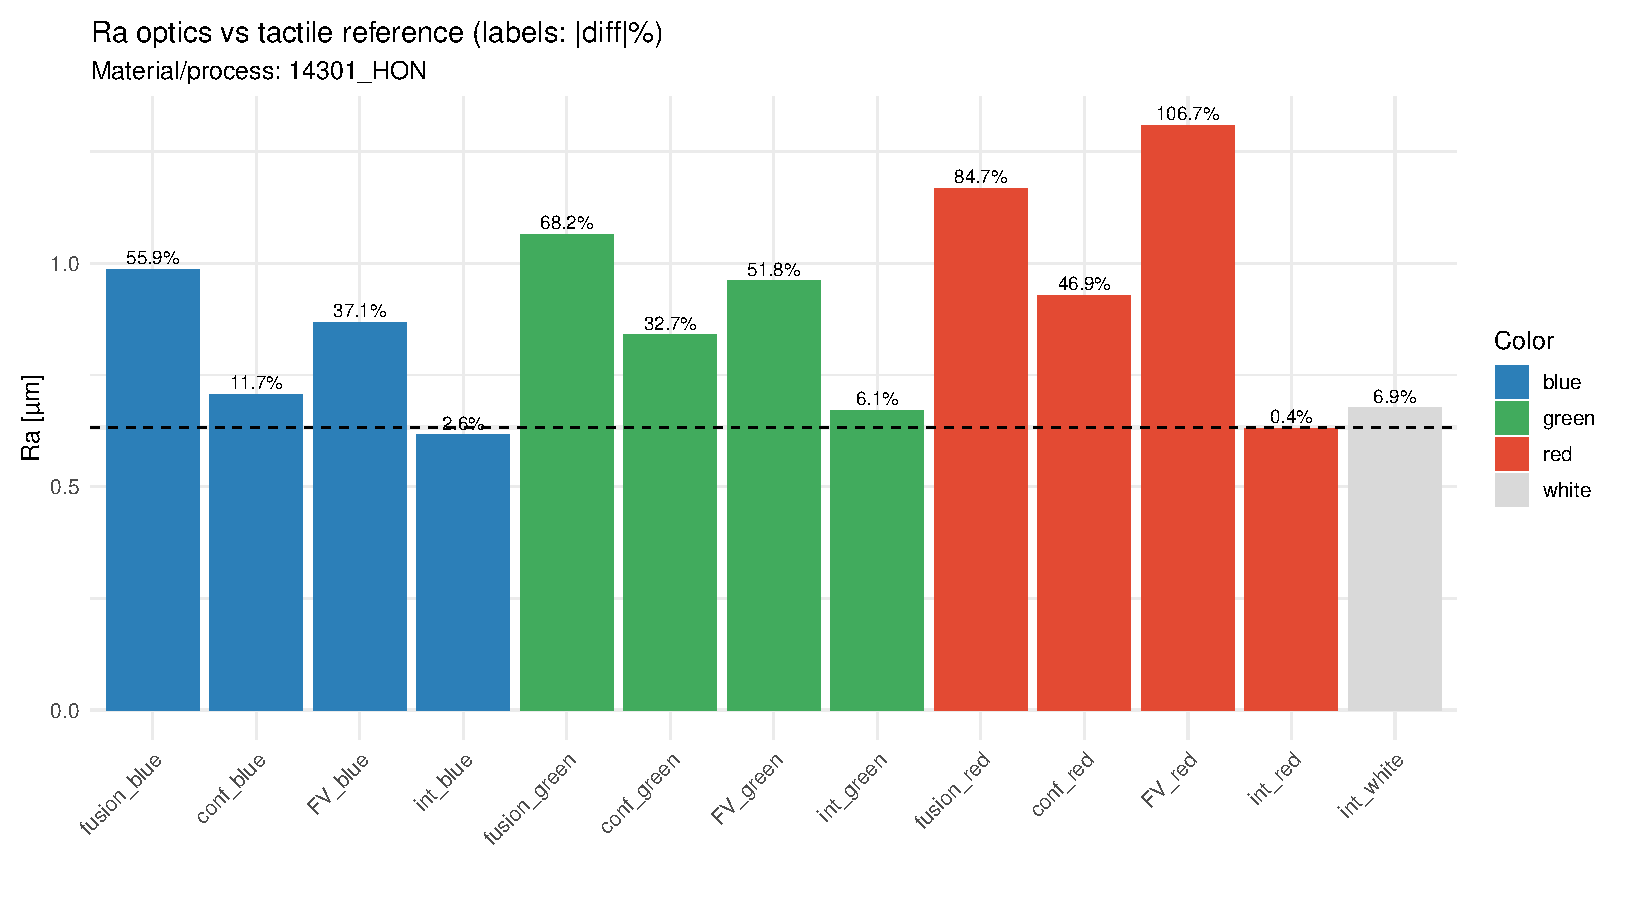
\includegraphics[width=\linewidth]{plots/ra_abs_14301_hon_optics_vs_tactile.pdf}
\end{minipage}
\begin{minipage}[t]{0.32\textwidth}\centering
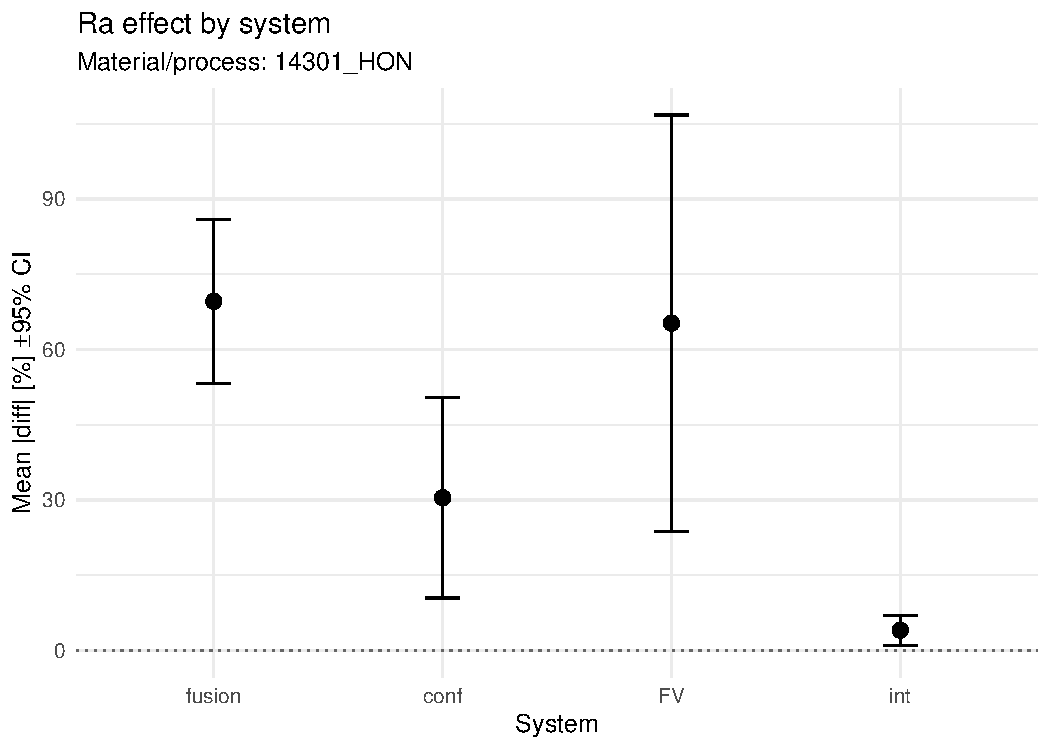
\includegraphics[width=\linewidth]{plots/ra_abs_14301_hon_effects_by_system.pdf}
\end{minipage}
\begin{minipage}[t]{0.32\textwidth}\centering
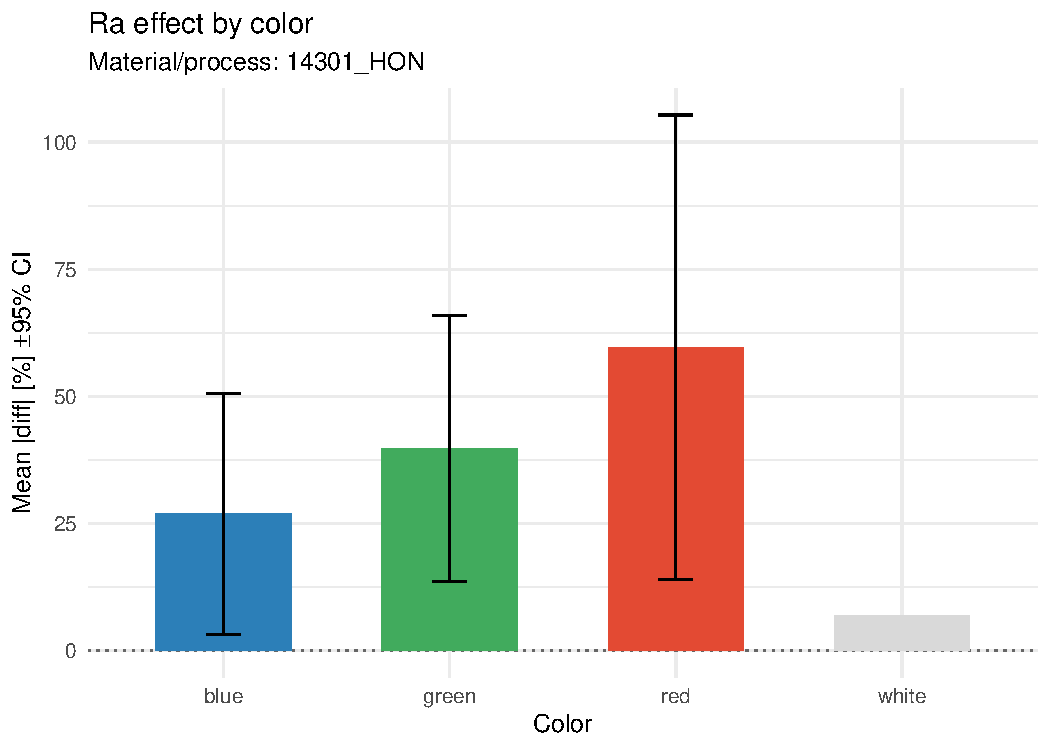
\includegraphics[width=\linewidth]{plots/ra_abs_14301_hon_effects_by_color.pdf}
\end{minipage}
\caption{RA — 14301\_hon — porównanie i efekty (|diff| \%)}
\end{figure}

\begin{figure}[H]\centering
\begin{minipage}[t]{0.32\textwidth}\centering
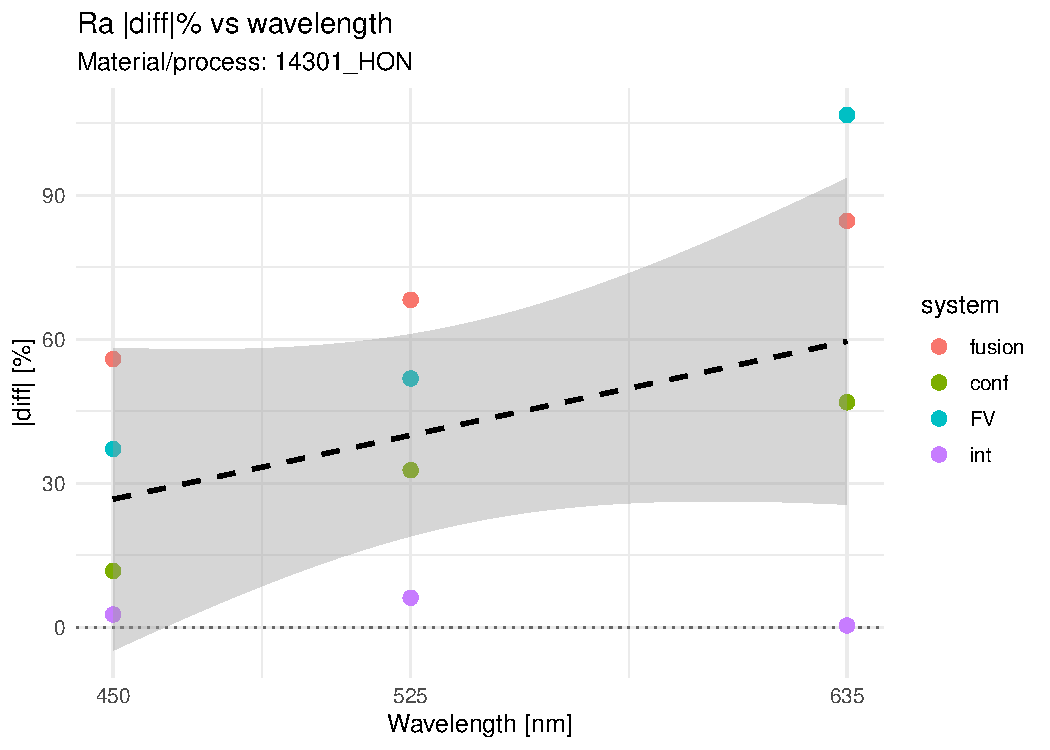
\includegraphics[width=\linewidth]{plots/ra_abs_14301_hon_diff_vs_wavelength.pdf}
\end{minipage}
\begin{minipage}[t]{0.32\textwidth}\centering
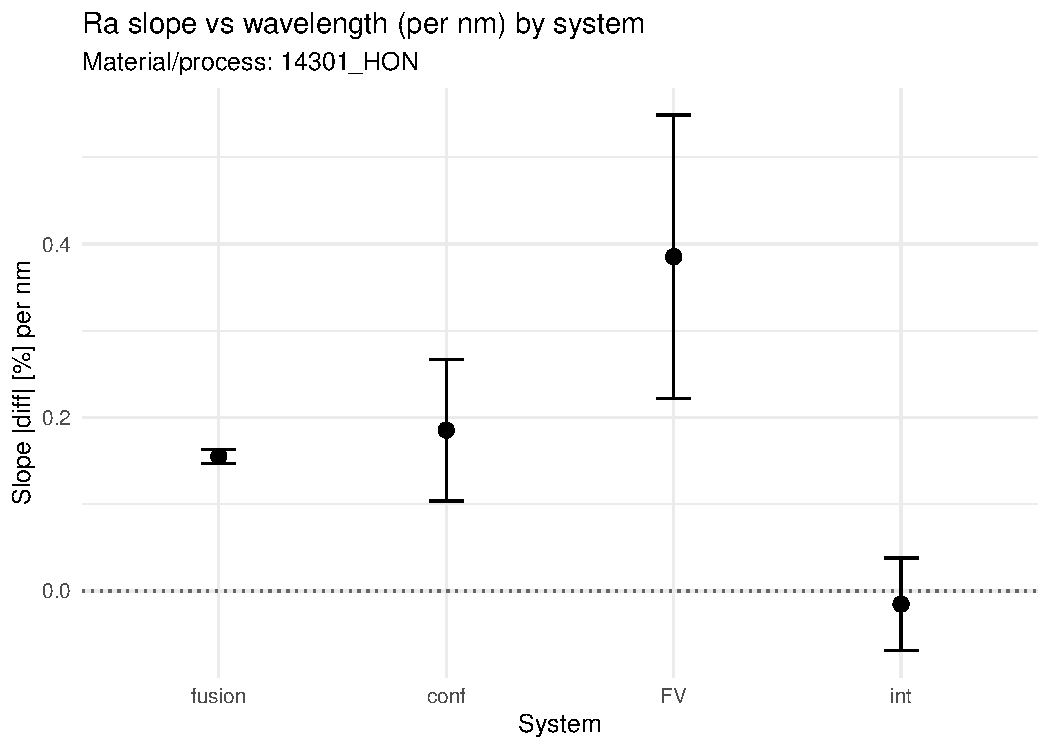
\includegraphics[width=\linewidth]{plots/ra_abs_14301_hon_slope_by_system_vs_nm.pdf}
\end{minipage}
\begin{minipage}[t]{0.32\textwidth}\centering
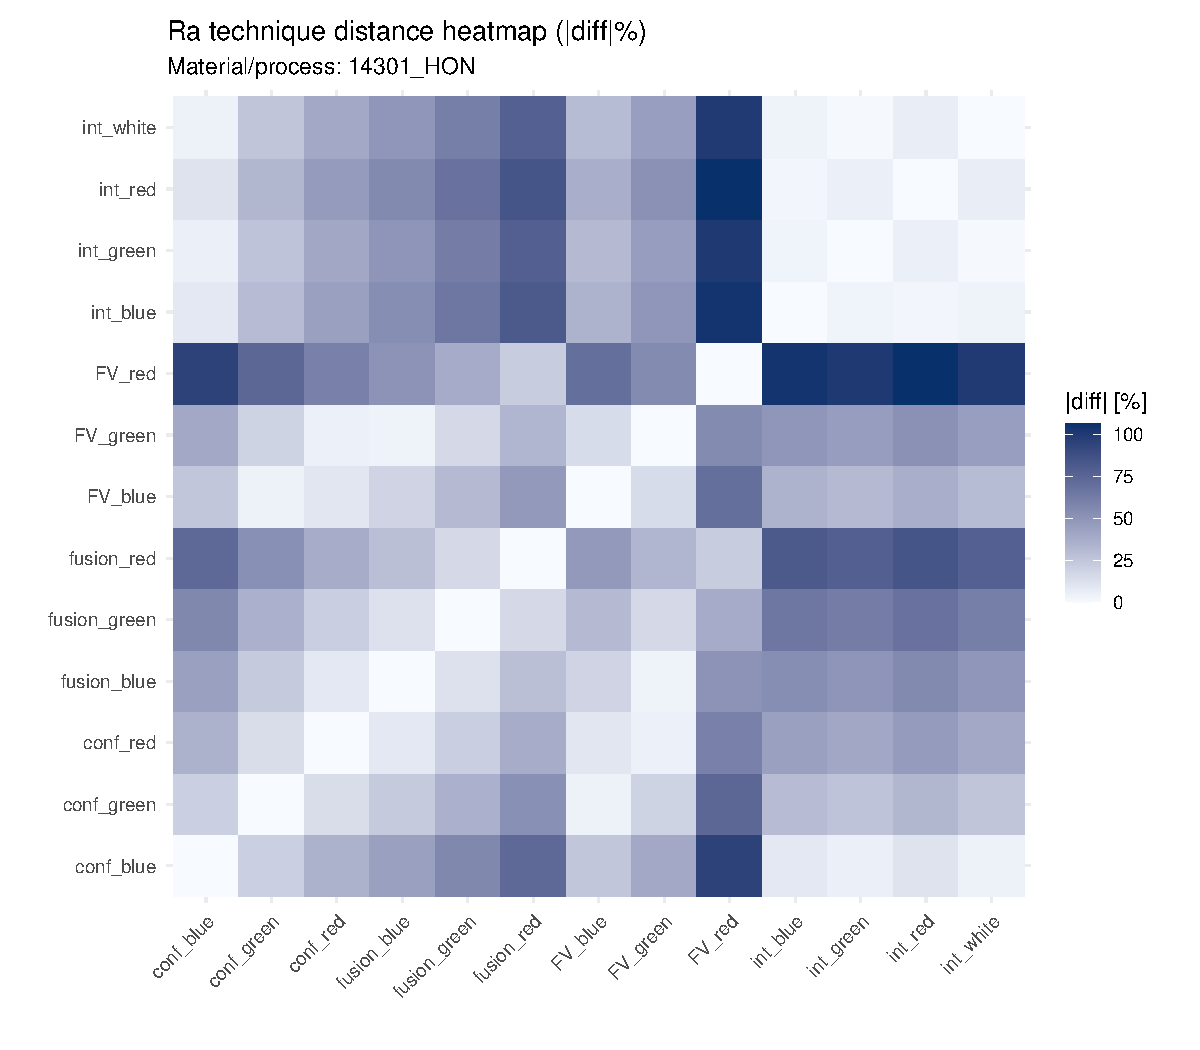
\includegraphics[width=\linewidth]{plots/ra_abs_14301_hon_tech_distance_heatmap.pdf}
\end{minipage}
\caption{RA — 14301\_hon — wavelength, nachylenia, odległości technik}
\end{figure}

\begin{figure}[H]\centering
\begin{minipage}[t]{0.32\textwidth}\centering
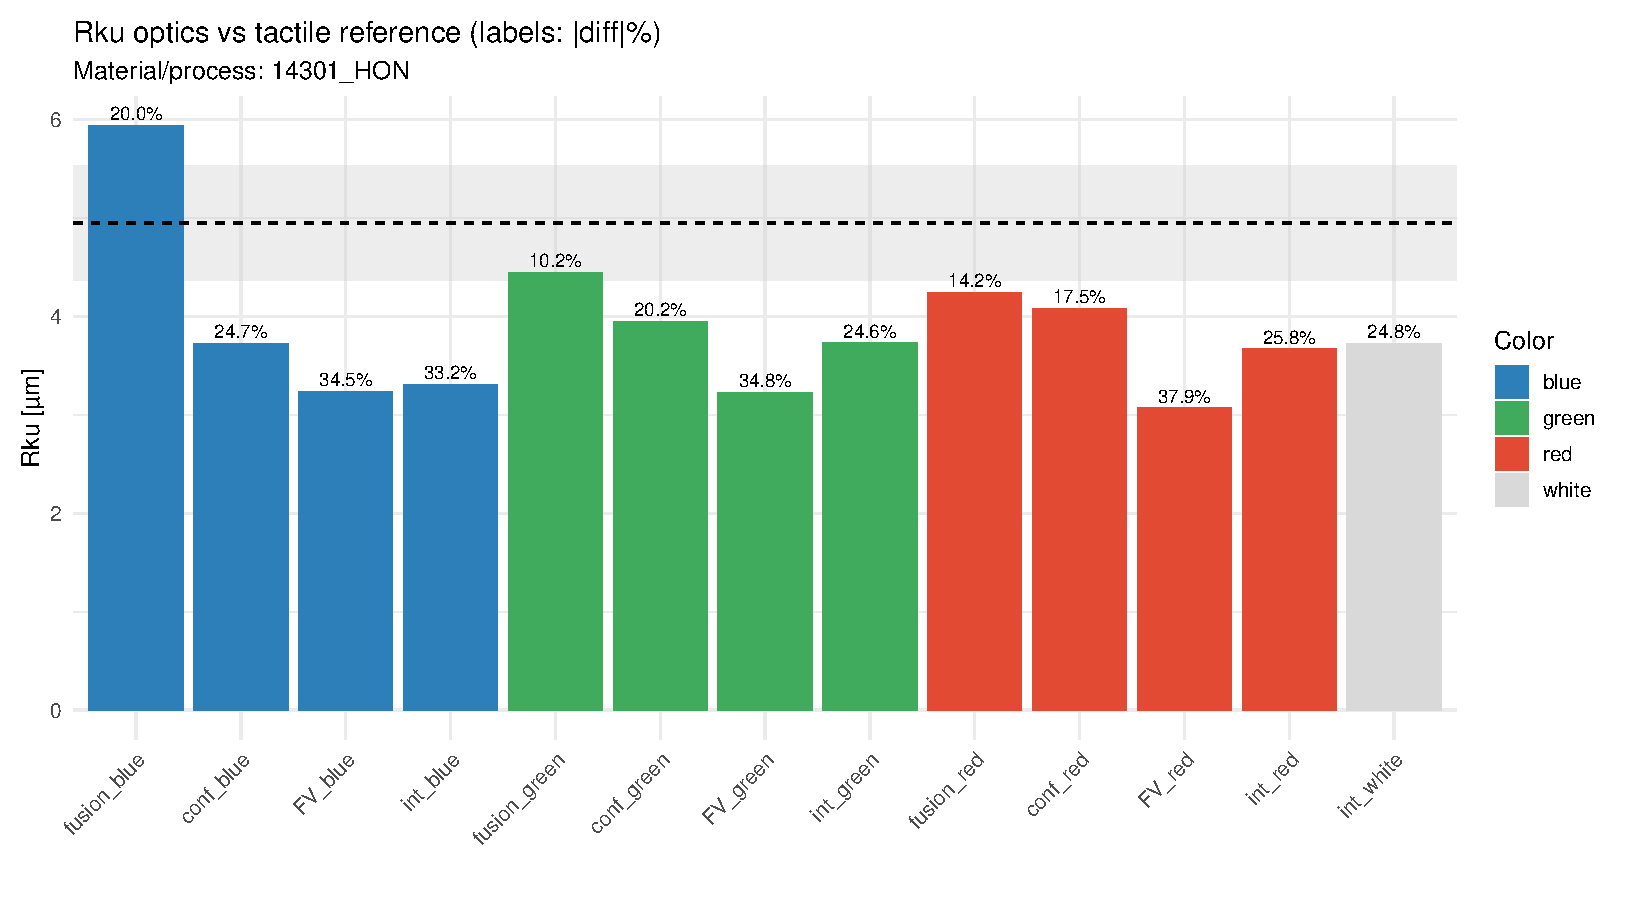
\includegraphics[width=\linewidth]{plots/rku_abs_14301_hon_optics_vs_tactile.pdf}
\end{minipage}
\begin{minipage}[t]{0.32\textwidth}\centering
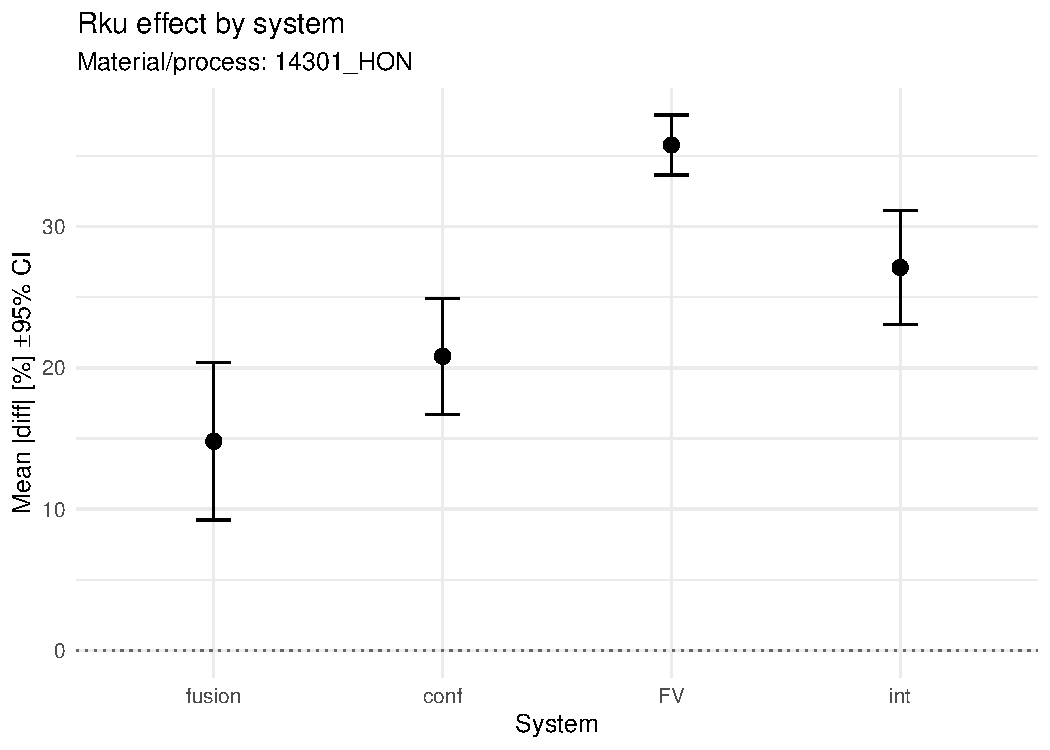
\includegraphics[width=\linewidth]{plots/rku_abs_14301_hon_effects_by_system.pdf}
\end{minipage}
\begin{minipage}[t]{0.32\textwidth}\centering
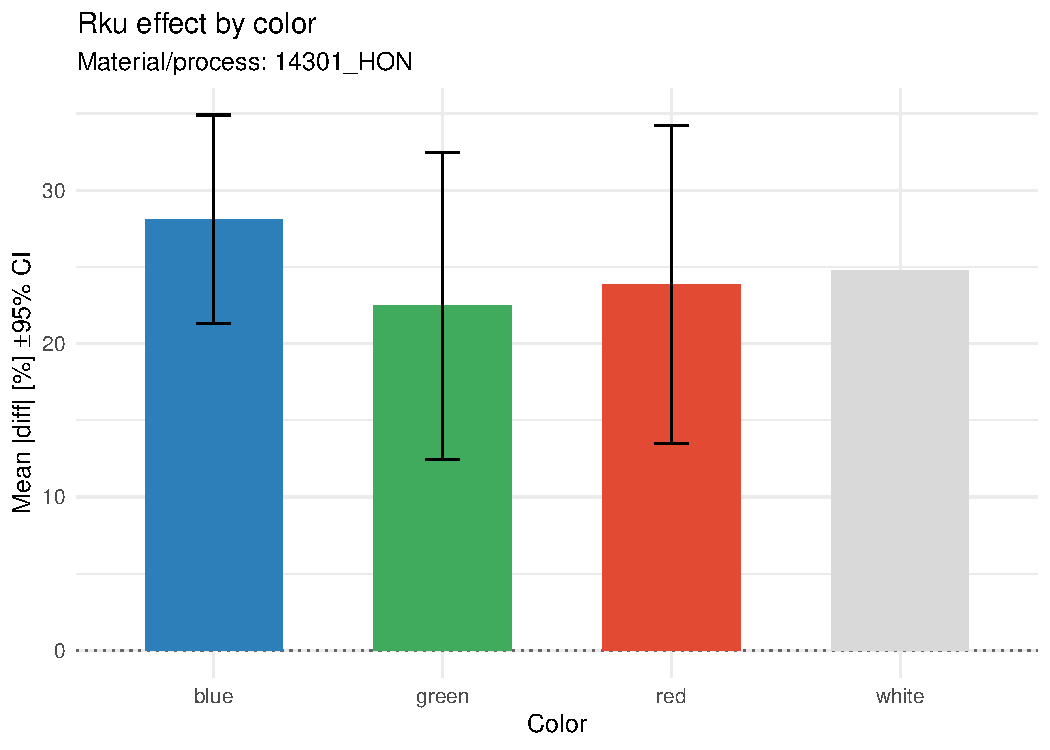
\includegraphics[width=\linewidth]{plots/rku_abs_14301_hon_effects_by_color.pdf}
\end{minipage}
\caption{RKU — 14301\_hon — porównanie i efekty (|diff| \%)}
\end{figure}

\begin{figure}[H]\centering
\begin{minipage}[t]{0.32\textwidth}\centering
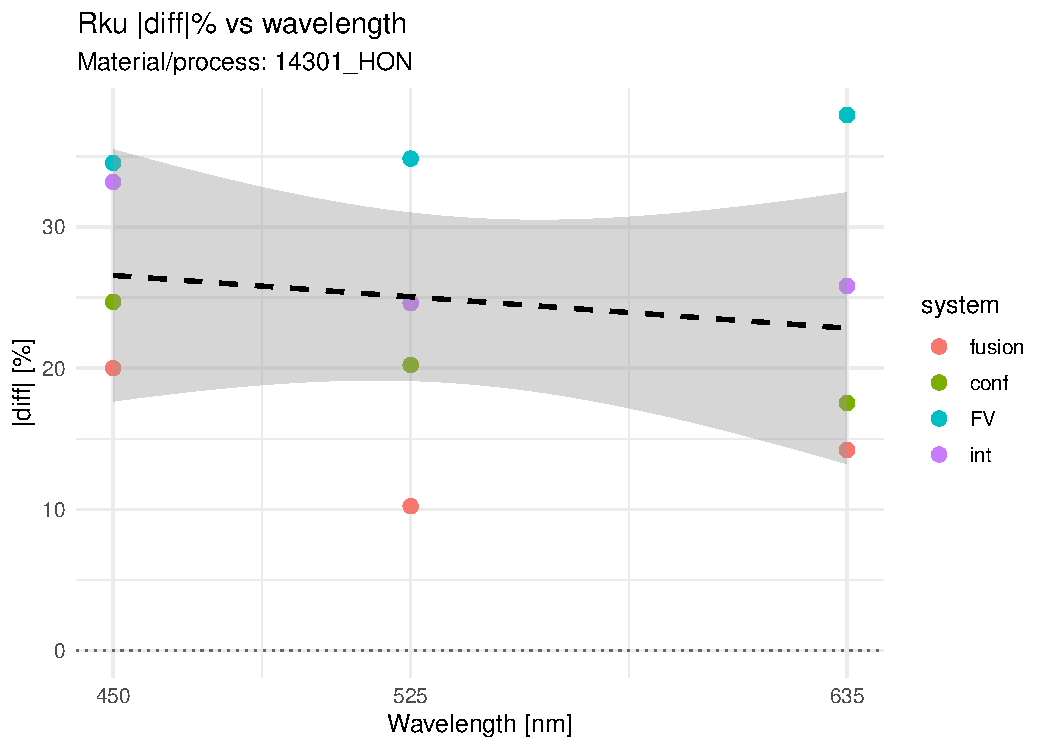
\includegraphics[width=\linewidth]{plots/rku_abs_14301_hon_diff_vs_wavelength.pdf}
\end{minipage}
\begin{minipage}[t]{0.32\textwidth}\centering
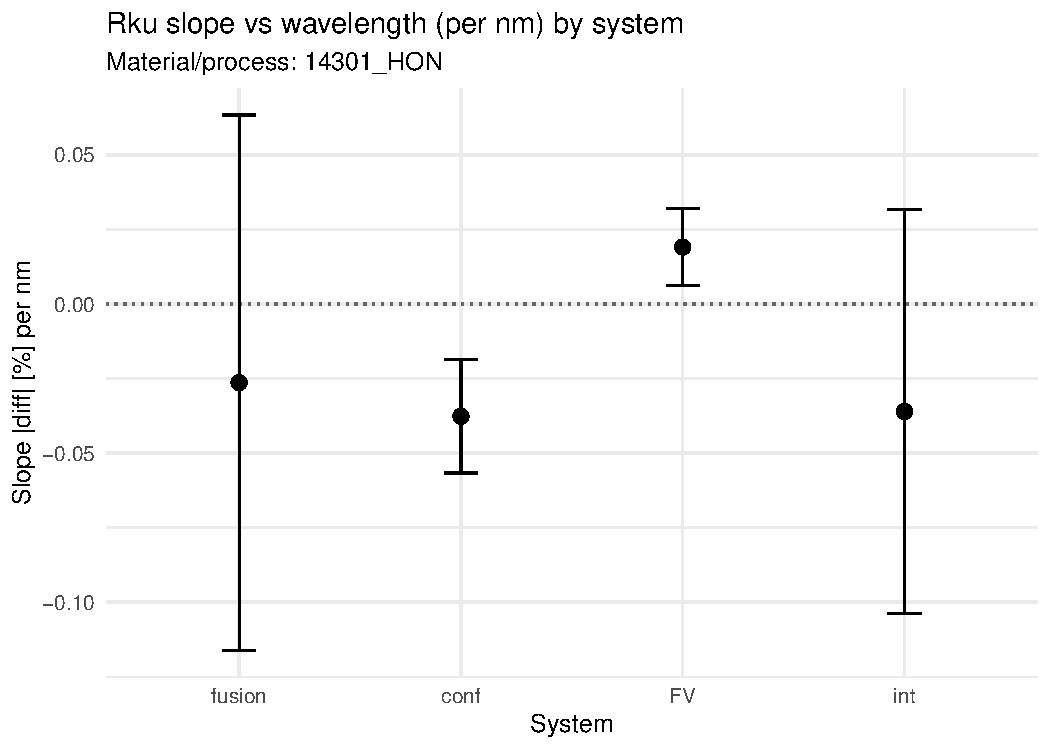
\includegraphics[width=\linewidth]{plots/rku_abs_14301_hon_slope_by_system_vs_nm.pdf}
\end{minipage}
\begin{minipage}[t]{0.32\textwidth}\centering
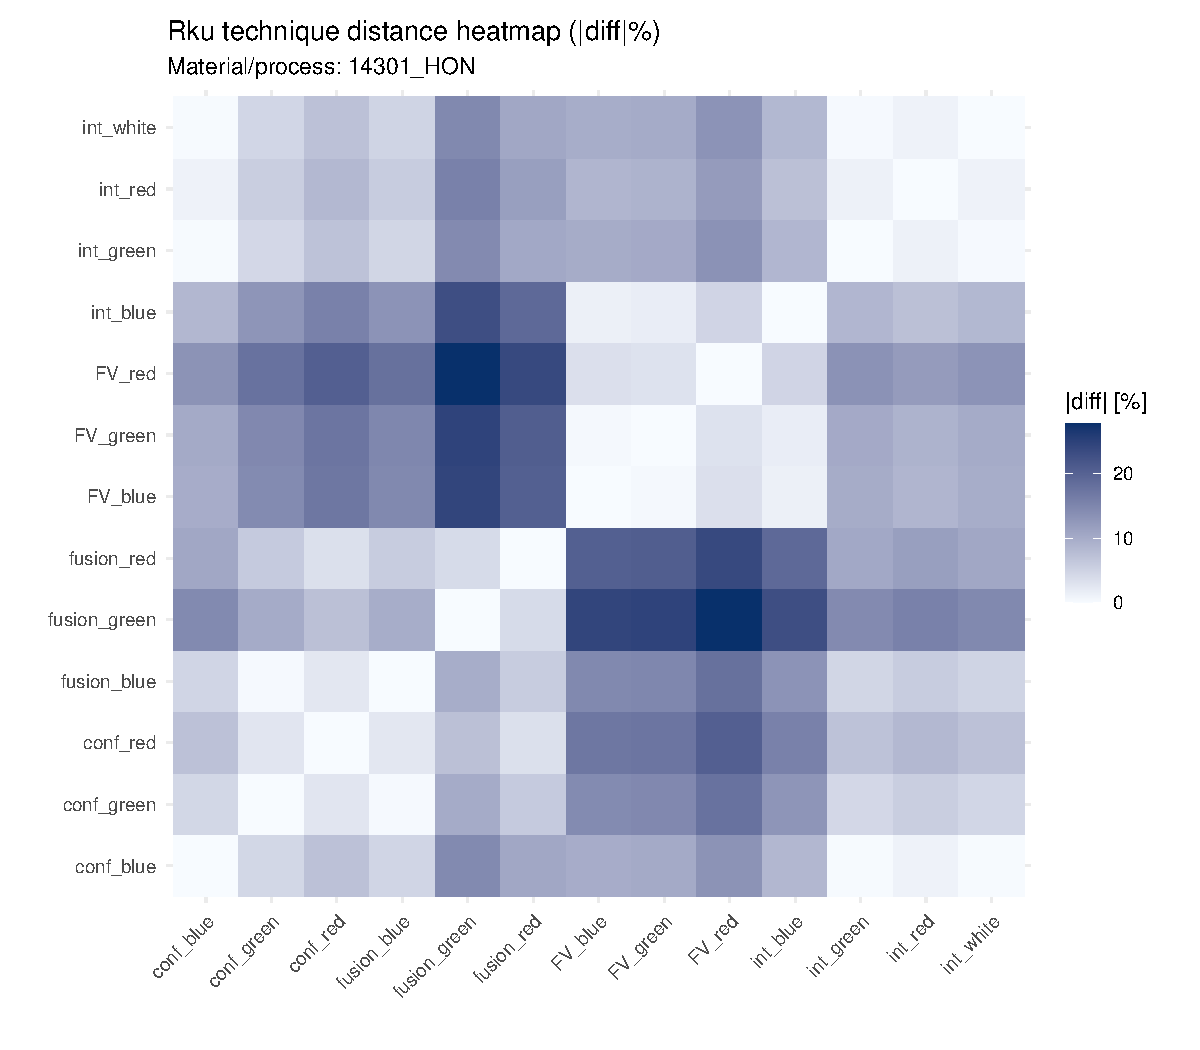
\includegraphics[width=\linewidth]{plots/rku_abs_14301_hon_tech_distance_heatmap.pdf}
\end{minipage}
\caption{RKU — 14301\_hon — wavelength, nachylenia, odległości technik}
\end{figure}

\begin{figure}[H]\centering
\begin{minipage}[t]{0.32\textwidth}\centering
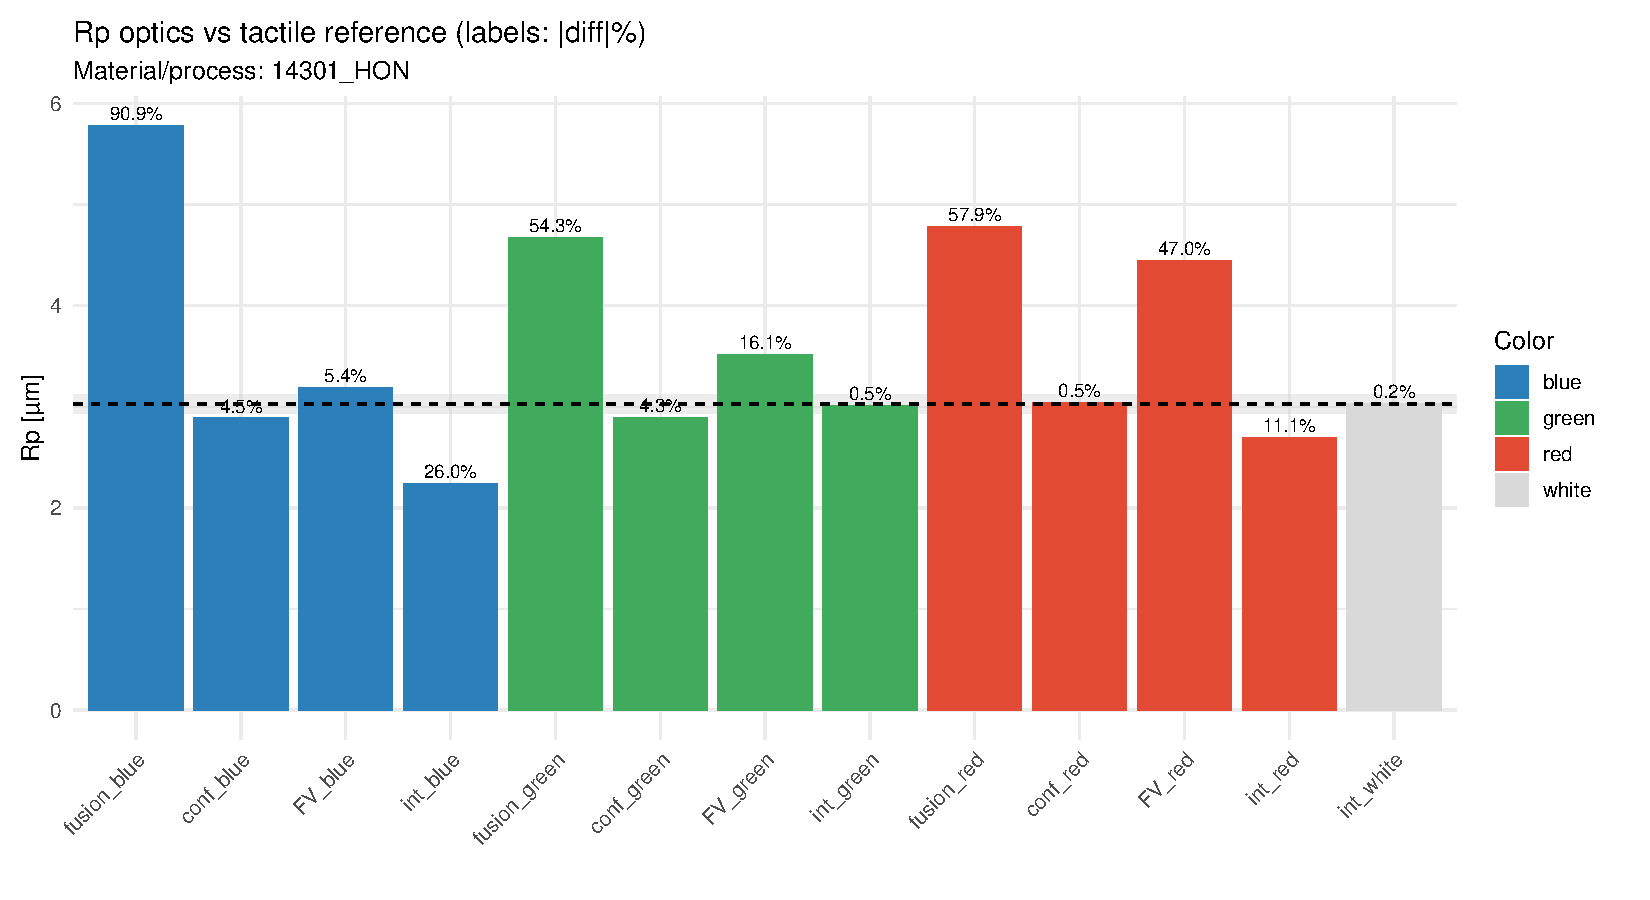
\includegraphics[width=\linewidth]{plots/rp_abs_14301_hon_optics_vs_tactile.pdf}
\end{minipage}
\begin{minipage}[t]{0.32\textwidth}\centering
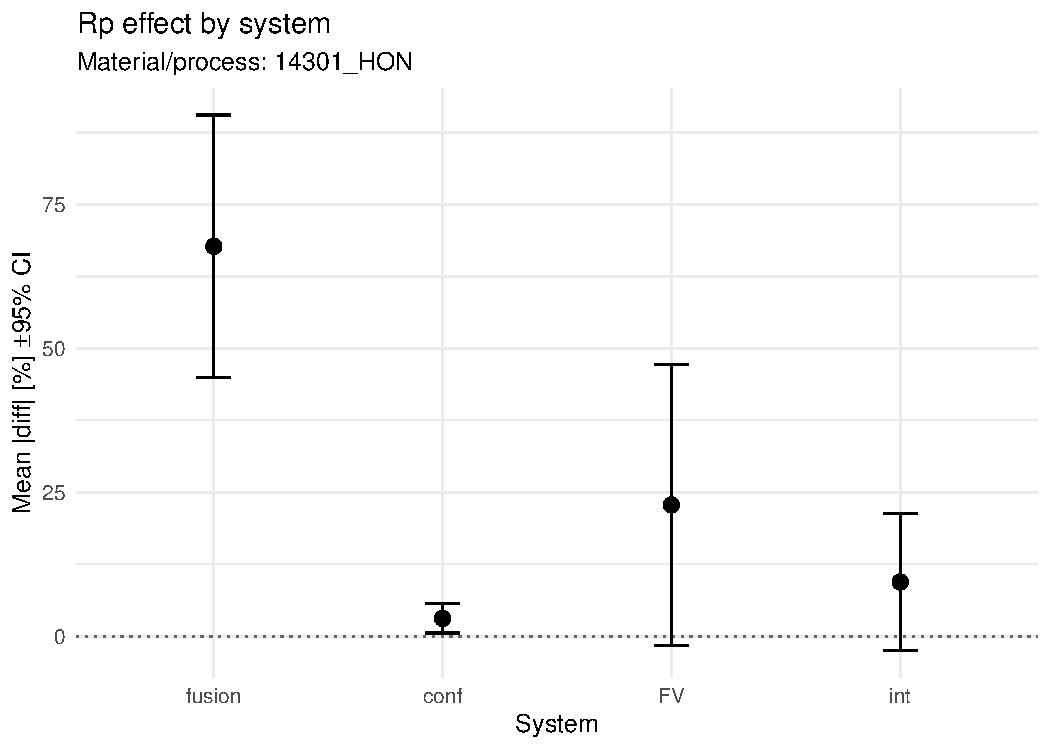
\includegraphics[width=\linewidth]{plots/rp_abs_14301_hon_effects_by_system.pdf}
\end{minipage}
\begin{minipage}[t]{0.32\textwidth}\centering
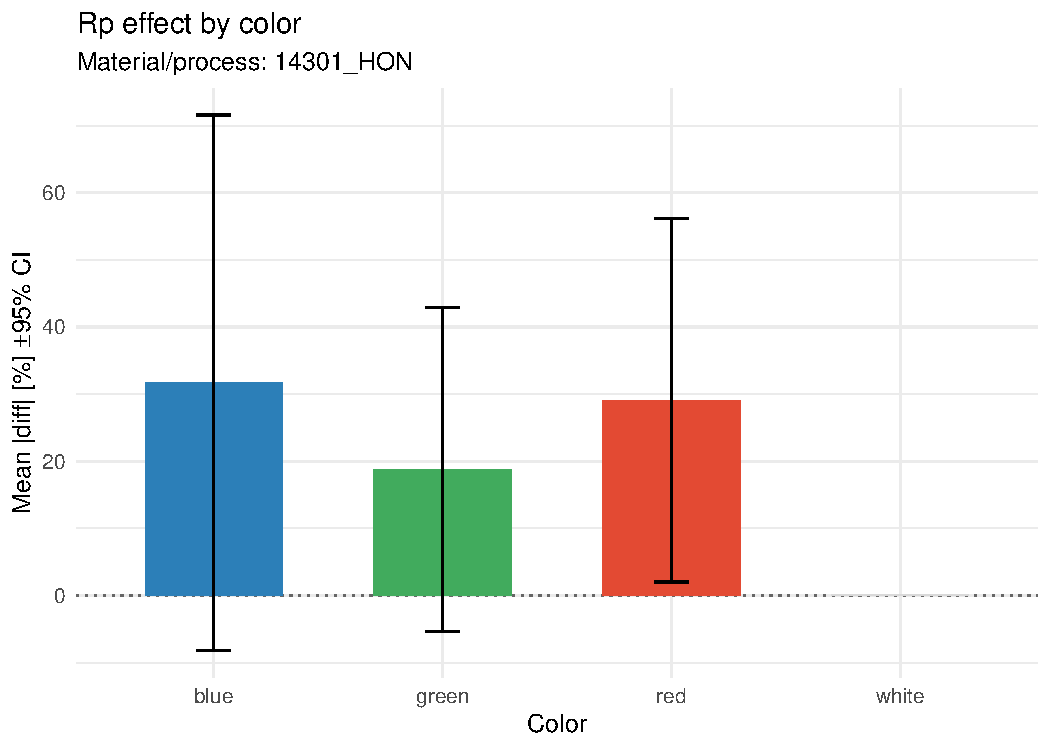
\includegraphics[width=\linewidth]{plots/rp_abs_14301_hon_effects_by_color.pdf}
\end{minipage}
\caption{RP — 14301\_hon — porównanie i efekty (|diff| \%)}
\end{figure}

\begin{figure}[H]\centering
\begin{minipage}[t]{0.32\textwidth}\centering
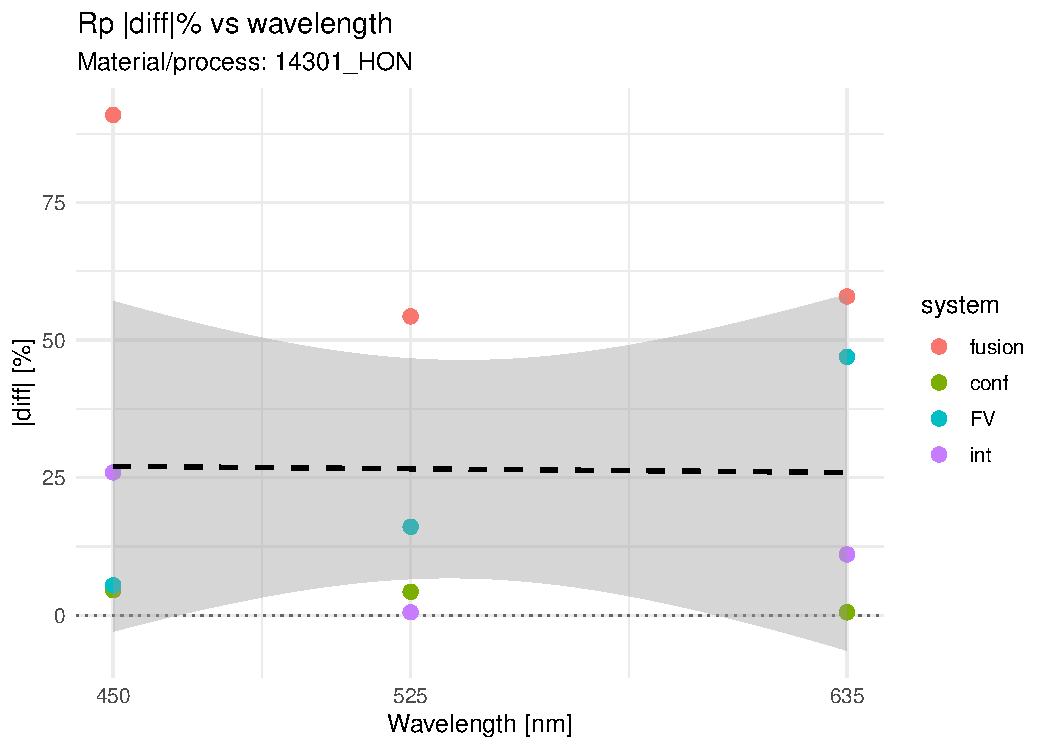
\includegraphics[width=\linewidth]{plots/rp_abs_14301_hon_diff_vs_wavelength.pdf}
\end{minipage}
\begin{minipage}[t]{0.32\textwidth}\centering
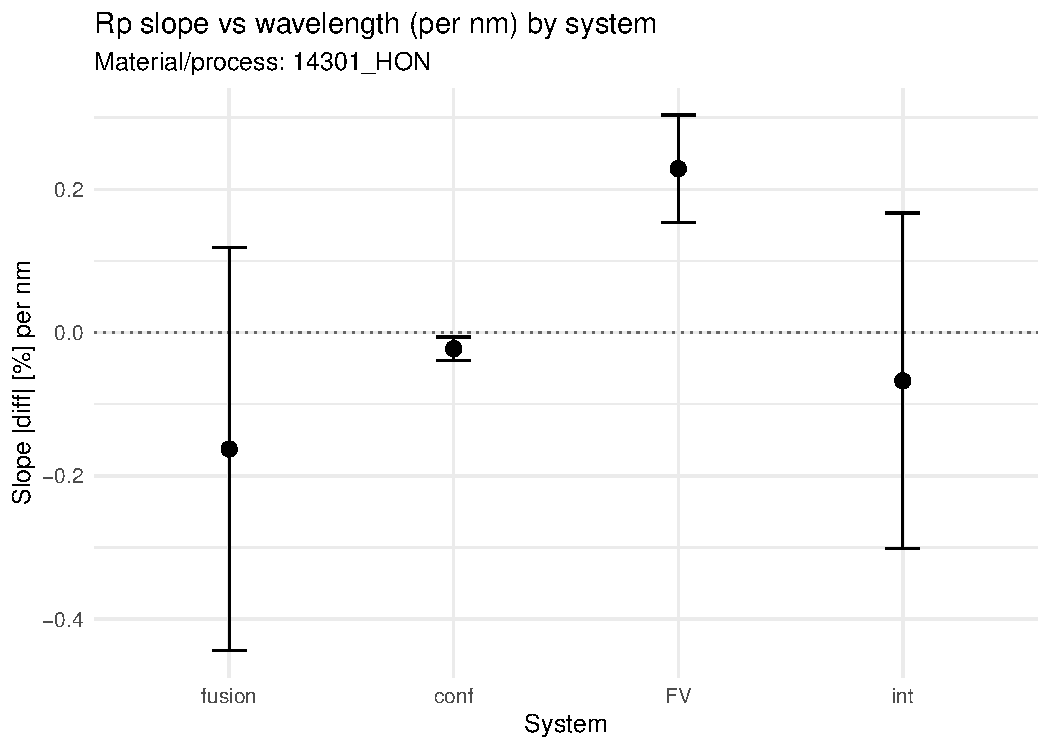
\includegraphics[width=\linewidth]{plots/rp_abs_14301_hon_slope_by_system_vs_nm.pdf}
\end{minipage}
\begin{minipage}[t]{0.32\textwidth}\centering
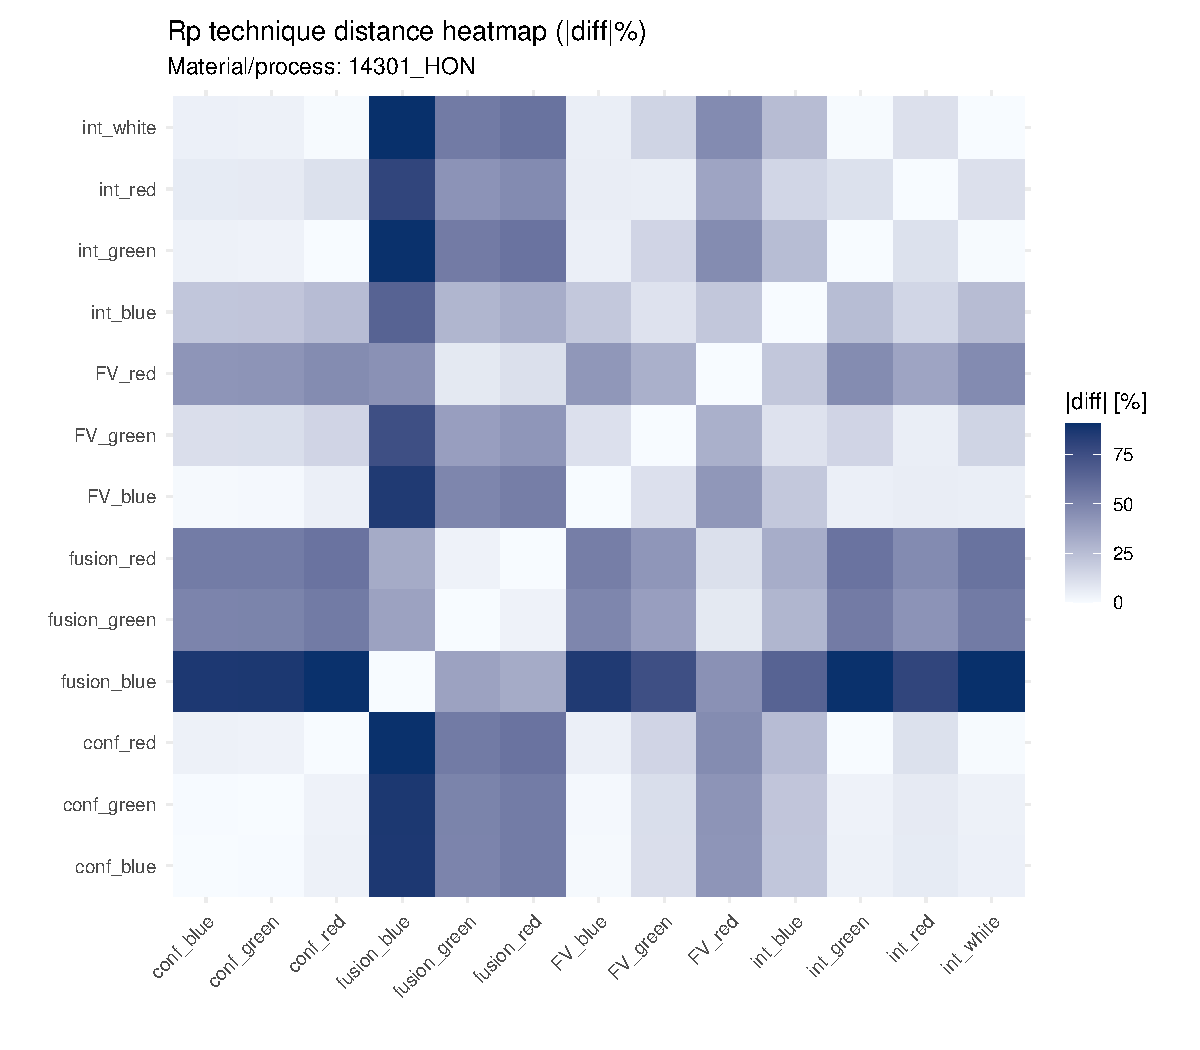
\includegraphics[width=\linewidth]{plots/rp_abs_14301_hon_tech_distance_heatmap.pdf}
\end{minipage}
\caption{RP — 14301\_hon — wavelength, nachylenia, odległości technik}
\end{figure}

\begin{figure}[H]\centering
\begin{minipage}[t]{0.32\textwidth}\centering
\includegraphics[width=\linewidth]{plots/rq_abs_14301_hon_optics_vs_tactile.pdf}
\end{minipage}
\begin{minipage}[t]{0.32\textwidth}\centering
\includegraphics[width=\linewidth]{plots/rq_abs_14301_hon_effects_by_system.pdf}
\end{minipage}
\begin{minipage}[t]{0.32\textwidth}\centering
\includegraphics[width=\linewidth]{plots/rq_abs_14301_hon_effects_by_color.pdf}
\end{minipage}
\caption{RQ — 14301\_hon — porównanie i efekty (|diff| \%)}
\end{figure}

\begin{figure}[H]\centering
\begin{minipage}[t]{0.32\textwidth}\centering
\includegraphics[width=\linewidth]{plots/rq_abs_14301_hon_diff_vs_wavelength.pdf}
\end{minipage}
\begin{minipage}[t]{0.32\textwidth}\centering
\includegraphics[width=\linewidth]{plots/rq_abs_14301_hon_slope_by_system_vs_nm.pdf}
\end{minipage}
\begin{minipage}[t]{0.32\textwidth}\centering
\includegraphics[width=\linewidth]{plots/rq_abs_14301_hon_tech_distance_heatmap.pdf}
\end{minipage}
\caption{RQ — 14301\_hon — wavelength, nachylenia, odległości technik}
\end{figure}

\begin{figure}[H]\centering
\begin{minipage}[t]{0.32\textwidth}\centering
\includegraphics[width=\linewidth]{plots/rsk_abs_14301_hon_optics_vs_tactile.pdf}
\end{minipage}
\begin{minipage}[t]{0.32\textwidth}\centering
\includegraphics[width=\linewidth]{plots/rsk_abs_14301_hon_effects_by_system.pdf}
\end{minipage}
\begin{minipage}[t]{0.32\textwidth}\centering
\includegraphics[width=\linewidth]{plots/rsk_abs_14301_hon_effects_by_color.pdf}
\end{minipage}
\caption{RSK — 14301\_hon — porównanie i efekty (|diff| \%)}
\end{figure}

\begin{figure}[H]\centering
\begin{minipage}[t]{0.32\textwidth}\centering
\includegraphics[width=\linewidth]{plots/rsk_abs_14301_hon_diff_vs_wavelength.pdf}
\end{minipage}
\begin{minipage}[t]{0.32\textwidth}\centering
\includegraphics[width=\linewidth]{plots/rsk_abs_14301_hon_slope_by_system_vs_nm.pdf}
\end{minipage}
\begin{minipage}[t]{0.32\textwidth}\centering
\includegraphics[width=\linewidth]{plots/rsk_abs_14301_hon_tech_distance_heatmap.pdf}
\end{minipage}
\caption{RSK — 14301\_hon — wavelength, nachylenia, odległości technik}
\end{figure}

\begin{figure}[H]\centering
\begin{minipage}[t]{0.32\textwidth}\centering
\includegraphics[width=\linewidth]{plots/rsm_abs_14301_hon_optics_vs_tactile.pdf}
\end{minipage}
\begin{minipage}[t]{0.32\textwidth}\centering
\includegraphics[width=\linewidth]{plots/rsm_abs_14301_hon_effects_by_system.pdf}
\end{minipage}
\begin{minipage}[t]{0.32\textwidth}\centering
\includegraphics[width=\linewidth]{plots/rsm_abs_14301_hon_effects_by_color.pdf}
\end{minipage}
\caption{RSM — 14301\_hon — porównanie i efekty (|diff| \%)}
\end{figure}

\begin{figure}[H]\centering
\begin{minipage}[t]{0.32\textwidth}\centering
\includegraphics[width=\linewidth]{plots/rsm_abs_14301_hon_diff_vs_wavelength.pdf}
\end{minipage}
\begin{minipage}[t]{0.32\textwidth}\centering
\includegraphics[width=\linewidth]{plots/rsm_abs_14301_hon_slope_by_system_vs_nm.pdf}
\end{minipage}
\begin{minipage}[t]{0.32\textwidth}\centering
\includegraphics[width=\linewidth]{plots/rsm_abs_14301_hon_tech_distance_heatmap.pdf}
\end{minipage}
\caption{RSM — 14301\_hon — wavelength, nachylenia, odległości technik}
\end{figure}

\begin{figure}[H]\centering
\begin{minipage}[t]{0.32\textwidth}\centering
\includegraphics[width=\linewidth]{plots/rt_abs_14301_hon_optics_vs_tactile.pdf}
\end{minipage}
\begin{minipage}[t]{0.32\textwidth}\centering
\includegraphics[width=\linewidth]{plots/rt_abs_14301_hon_effects_by_system.pdf}
\end{minipage}
\begin{minipage}[t]{0.32\textwidth}\centering
\includegraphics[width=\linewidth]{plots/rt_abs_14301_hon_effects_by_color.pdf}
\end{minipage}
\caption{RT — 14301\_hon — porównanie i efekty (|diff| \%)}
\end{figure}

\begin{figure}[H]\centering
\begin{minipage}[t]{0.32\textwidth}\centering
\includegraphics[width=\linewidth]{plots/rt_abs_14301_hon_diff_vs_wavelength.pdf}
\end{minipage}
\begin{minipage}[t]{0.32\textwidth}\centering
\includegraphics[width=\linewidth]{plots/rt_abs_14301_hon_slope_by_system_vs_nm.pdf}
\end{minipage}
\begin{minipage}[t]{0.32\textwidth}\centering
\includegraphics[width=\linewidth]{plots/rt_abs_14301_hon_tech_distance_heatmap.pdf}
\end{minipage}
\caption{RT — 14301\_hon — wavelength, nachylenia, odległości technik}
\end{figure}

\begin{figure}[H]\centering
\begin{minipage}[t]{0.32\textwidth}\centering
\includegraphics[width=\linewidth]{plots/rv_abs_14301_hon_optics_vs_tactile.pdf}
\end{minipage}
\begin{minipage}[t]{0.32\textwidth}\centering
\includegraphics[width=\linewidth]{plots/rv_abs_14301_hon_effects_by_system.pdf}
\end{minipage}
\begin{minipage}[t]{0.32\textwidth}\centering
\includegraphics[width=\linewidth]{plots/rv_abs_14301_hon_effects_by_color.pdf}
\end{minipage}
\caption{RV — 14301\_hon — porównanie i efekty (|diff| \%)}
\end{figure}

\begin{figure}[H]\centering
\begin{minipage}[t]{0.32\textwidth}\centering
\includegraphics[width=\linewidth]{plots/rv_abs_14301_hon_diff_vs_wavelength.pdf}
\end{minipage}
\begin{minipage}[t]{0.32\textwidth}\centering
\includegraphics[width=\linewidth]{plots/rv_abs_14301_hon_slope_by_system_vs_nm.pdf}
\end{minipage}
\begin{minipage}[t]{0.32\textwidth}\centering
\includegraphics[width=\linewidth]{plots/rv_abs_14301_hon_tech_distance_heatmap.pdf}
\end{minipage}
\caption{RV — 14301\_hon — wavelength, nachylenia, odległości technik}
\end{figure}

\begin{figure}[H]\centering
\begin{minipage}[t]{0.32\textwidth}\centering
\includegraphics[width=\linewidth]{plots/rz_abs_14301_hon_optics_vs_tactile.pdf}
\end{minipage}
\begin{minipage}[t]{0.32\textwidth}\centering
\includegraphics[width=\linewidth]{plots/rz_abs_14301_hon_effects_by_system.pdf}
\end{minipage}
\begin{minipage}[t]{0.32\textwidth}\centering
\includegraphics[width=\linewidth]{plots/rz_abs_14301_hon_effects_by_color.pdf}
\end{minipage}
\caption{RZ — 14301\_hon — porównanie i efekty (|diff| \%)}
\end{figure}

\begin{figure}[H]\centering
\begin{minipage}[t]{0.32\textwidth}\centering
\includegraphics[width=\linewidth]{plots/rz_abs_14301_hon_diff_vs_wavelength.pdf}
\end{minipage}
\begin{minipage}[t]{0.32\textwidth}\centering
\includegraphics[width=\linewidth]{plots/rz_abs_14301_hon_slope_by_system_vs_nm.pdf}
\end{minipage}
\begin{minipage}[t]{0.32\textwidth}\centering
\includegraphics[width=\linewidth]{plots/rz_abs_14301_hon_tech_distance_heatmap.pdf}
\end{minipage}
\caption{RZ — 14301\_hon — wavelength, nachylenia, odległości technik}
\end{figure}

\begin{figure}[H]\centering
\begin{minipage}[t]{0.32\textwidth}\centering
\includegraphics[width=\linewidth]{plots/rz1max_abs_14301_hon_optics_vs_tactile.pdf}
\end{minipage}
\begin{minipage}[t]{0.32\textwidth}\centering
\includegraphics[width=\linewidth]{plots/rz1max_abs_14301_hon_effects_by_system.pdf}
\end{minipage}
\begin{minipage}[t]{0.32\textwidth}\centering
\includegraphics[width=\linewidth]{plots/rz1max_abs_14301_hon_effects_by_color.pdf}
\end{minipage}
\caption{RZ1MAX — 14301\_hon — porównanie i efekty (|diff| \%)}
\end{figure}

\begin{figure}[H]\centering
\begin{minipage}[t]{0.32\textwidth}\centering
\includegraphics[width=\linewidth]{plots/rz1max_abs_14301_hon_diff_vs_wavelength.pdf}
\end{minipage}
\begin{minipage}[t]{0.32\textwidth}\centering
\includegraphics[width=\linewidth]{plots/rz1max_abs_14301_hon_slope_by_system_vs_nm.pdf}
\end{minipage}
\begin{minipage}[t]{0.32\textwidth}\centering
\includegraphics[width=\linewidth]{plots/rz1max_abs_14301_hon_tech_distance_heatmap.pdf}
\end{minipage}
\caption{RZ1MAX — 14301\_hon — wavelength, nachylenia, odległości technik}
\end{figure}

\subsection{Wyniki i wnioski dla materiał/proces: 14301\_hon}

\textbf{RA}. r=0.416, rho=0.296; eta2: system=0.726, color=0.160.
Istotne nachylenia: fusion(slope=0.155, p=0.017). Wniosek: TAK.
\textbf{RKU}. r=-0.181, rho=-0.148; eta2: system=0.847, color=0.088.
Wniosek: NIE. \textbf{RP}. r=-0.016, rho=-0.059; eta2: system=0.782,
color=0.048. Wniosek: NIE. \textbf{RQ}. r=0.373, rho=0.296; eta2:
system=0.759, color=0.128. Wniosek: NIE. \textbf{RSK}. r=0.412,
rho=0.414; eta2: system=0.586, color=0.176. Wniosek: NIE. \textbf{RSM}.
r=0.158, rho=0.177; eta2: system=0.917, color=0.046. Wniosek: NIE.
\textbf{RT}. r=0.305, rho=0.384; eta2: system=0.686, color=0.120. Trendy
(p\textless0.1): fusion(slope=0.087, p=0.090). Wniosek: NIE.
\textbf{RV}. r=0.425, rho=0.384; eta2: system=0.752, color=0.166.
Wniosek: NIE. \textbf{RZ}. r=0.286, rho=0.266; eta2: system=0.844,
color=0.079. Trendy (p\textless0.1): fusion(slope=0.094, p=0.062).
Wniosek: NIE. \textbf{RZ1MAX}. r=0.293, rho=0.414; eta2: system=0.694,
color=0.115. Istotne nachylenia: fusion(slope=0.082, p=0.030). Wniosek:
TAK.

\paragraph{Podsumowanie (opisowe) dla tego materiału/procesu}
\begin{itemize}
\item W ujęciu ANOVA: częściej dominuje system (eta²).
\item Najczęściej preferowany system (min średni |diff|): int.
\item Najczęściej preferowana barwa (min średni |diff|): white.
\item Zależność od wavelength wykryta (p<0.05) dla parametrów: RA, RZ1MAX; dotyczy systemów: fusion.
\end{itemize}
\paragraph{Rekomendacje dla tego materiału}
\begin{itemize}
\item RA: preferowany system (min średni |diff|): int; preferowana barwa (min średni |diff|): white; dominuje system; zależność od wavelength: TAK (p<0.05) — fusion: rośnie.
\item RKU: preferowany system (min średni |diff|): fusion; preferowana barwa (min średni |diff|): green; dominuje system; zależność od wavelength: NIE (brak wykrytego trendu per system).
\item RP: preferowany system (min średni |diff|): conf; preferowana barwa (min średni |diff|): white; dominuje system; zależność od wavelength: NIE (brak wykrytego trendu per system).
\item RQ: preferowany system (min średni |diff|): int; preferowana barwa (min średni |diff|): white; dominuje system; zależność od wavelength: NIE (brak wykrytego trendu per system).
\item RSK: preferowany system (min średni |diff|): int; preferowana barwa (min średni |diff|): white; dominuje system; zależność od wavelength: NIE (brak wykrytego trendu per system).
\item RSM: preferowany system (min średni |diff|): FV; preferowana barwa (min średni |diff|): blue; dominuje system; zależność od wavelength: NIE (brak wykrytego trendu per system).
\item RT: preferowany system (min średni |diff|): conf; preferowana barwa (min średni |diff|): white; dominuje system; zależność od wavelength: trend (p<0.1) — fusion: rośnie.
\item RV: preferowany system (min średni |diff|): int; preferowana barwa (min średni |diff|): white; dominuje system; zależność od wavelength: NIE (brak wykrytego trendu per system).
\item RZ: preferowany system (min średni |diff|): int; preferowana barwa (min średni |diff|): white; dominuje system; zależność od wavelength: trend (p<0.1) — fusion: rośnie.
\item RZ1MAX: preferowany system (min średni |diff|): conf; preferowana barwa (min średni |diff|): white; dominuje system; zależność od wavelength: TAK (p<0.05) — fusion: rośnie.
\end{itemize}
\subsubsection{Materiał/proces: 14301\_mf}
\begin{figure}[H]\centering
\begin{minipage}[t]{0.32\textwidth}\centering
\includegraphics[width=\linewidth]{plots/ra_abs_14301_mf_optics_vs_tactile.pdf}
\end{minipage}
\begin{minipage}[t]{0.32\textwidth}\centering
\includegraphics[width=\linewidth]{plots/ra_abs_14301_mf_effects_by_system.pdf}
\end{minipage}
\begin{minipage}[t]{0.32\textwidth}\centering
\includegraphics[width=\linewidth]{plots/ra_abs_14301_mf_effects_by_color.pdf}
\end{minipage}
\caption{RA — 14301\_mf — porównanie i efekty (|diff| \%)}
\end{figure}

\begin{figure}[H]\centering
\begin{minipage}[t]{0.32\textwidth}\centering
\includegraphics[width=\linewidth]{plots/ra_abs_14301_mf_diff_vs_wavelength.pdf}
\end{minipage}
\begin{minipage}[t]{0.32\textwidth}\centering
\includegraphics[width=\linewidth]{plots/ra_abs_14301_mf_slope_by_system_vs_nm.pdf}
\end{minipage}
\begin{minipage}[t]{0.32\textwidth}\centering
\includegraphics[width=\linewidth]{plots/ra_abs_14301_mf_tech_distance_heatmap.pdf}
\end{minipage}
\caption{RA — 14301\_mf — wavelength, nachylenia, odległości technik}
\end{figure}

\begin{figure}[H]\centering
\begin{minipage}[t]{0.32\textwidth}\centering
\includegraphics[width=\linewidth]{plots/rku_abs_14301_mf_optics_vs_tactile.pdf}
\end{minipage}
\begin{minipage}[t]{0.32\textwidth}\centering
\includegraphics[width=\linewidth]{plots/rku_abs_14301_mf_effects_by_system.pdf}
\end{minipage}
\begin{minipage}[t]{0.32\textwidth}\centering
\includegraphics[width=\linewidth]{plots/rku_abs_14301_mf_effects_by_color.pdf}
\end{minipage}
\caption{RKU — 14301\_mf — porównanie i efekty (|diff| \%)}
\end{figure}

\begin{figure}[H]\centering
\begin{minipage}[t]{0.32\textwidth}\centering
\includegraphics[width=\linewidth]{plots/rku_abs_14301_mf_diff_vs_wavelength.pdf}
\end{minipage}
\begin{minipage}[t]{0.32\textwidth}\centering
\includegraphics[width=\linewidth]{plots/rku_abs_14301_mf_slope_by_system_vs_nm.pdf}
\end{minipage}
\begin{minipage}[t]{0.32\textwidth}\centering
\includegraphics[width=\linewidth]{plots/rku_abs_14301_mf_tech_distance_heatmap.pdf}
\end{minipage}
\caption{RKU — 14301\_mf — wavelength, nachylenia, odległości technik}
\end{figure}

\begin{figure}[H]\centering
\begin{minipage}[t]{0.32\textwidth}\centering
\includegraphics[width=\linewidth]{plots/rp_abs_14301_mf_optics_vs_tactile.pdf}
\end{minipage}
\begin{minipage}[t]{0.32\textwidth}\centering
\includegraphics[width=\linewidth]{plots/rp_abs_14301_mf_effects_by_system.pdf}
\end{minipage}
\begin{minipage}[t]{0.32\textwidth}\centering
\includegraphics[width=\linewidth]{plots/rp_abs_14301_mf_effects_by_color.pdf}
\end{minipage}
\caption{RP — 14301\_mf — porównanie i efekty (|diff| \%)}
\end{figure}

\begin{figure}[H]\centering
\begin{minipage}[t]{0.32\textwidth}\centering
\includegraphics[width=\linewidth]{plots/rp_abs_14301_mf_diff_vs_wavelength.pdf}
\end{minipage}
\begin{minipage}[t]{0.32\textwidth}\centering
\includegraphics[width=\linewidth]{plots/rp_abs_14301_mf_slope_by_system_vs_nm.pdf}
\end{minipage}
\begin{minipage}[t]{0.32\textwidth}\centering
\includegraphics[width=\linewidth]{plots/rp_abs_14301_mf_tech_distance_heatmap.pdf}
\end{minipage}
\caption{RP — 14301\_mf — wavelength, nachylenia, odległości technik}
\end{figure}

\begin{figure}[H]\centering
\begin{minipage}[t]{0.32\textwidth}\centering
\includegraphics[width=\linewidth]{plots/rq_abs_14301_mf_optics_vs_tactile.pdf}
\end{minipage}
\begin{minipage}[t]{0.32\textwidth}\centering
\includegraphics[width=\linewidth]{plots/rq_abs_14301_mf_effects_by_system.pdf}
\end{minipage}
\begin{minipage}[t]{0.32\textwidth}\centering
\includegraphics[width=\linewidth]{plots/rq_abs_14301_mf_effects_by_color.pdf}
\end{minipage}
\caption{RQ — 14301\_mf — porównanie i efekty (|diff| \%)}
\end{figure}

\begin{figure}[H]\centering
\begin{minipage}[t]{0.32\textwidth}\centering
\includegraphics[width=\linewidth]{plots/rq_abs_14301_mf_diff_vs_wavelength.pdf}
\end{minipage}
\begin{minipage}[t]{0.32\textwidth}\centering
\includegraphics[width=\linewidth]{plots/rq_abs_14301_mf_slope_by_system_vs_nm.pdf}
\end{minipage}
\begin{minipage}[t]{0.32\textwidth}\centering
\includegraphics[width=\linewidth]{plots/rq_abs_14301_mf_tech_distance_heatmap.pdf}
\end{minipage}
\caption{RQ — 14301\_mf — wavelength, nachylenia, odległości technik}
\end{figure}

\begin{figure}[H]\centering
\begin{minipage}[t]{0.32\textwidth}\centering
\includegraphics[width=\linewidth]{plots/rsk_abs_14301_mf_optics_vs_tactile.pdf}
\end{minipage}
\begin{minipage}[t]{0.32\textwidth}\centering
\includegraphics[width=\linewidth]{plots/rsk_abs_14301_mf_effects_by_system.pdf}
\end{minipage}
\begin{minipage}[t]{0.32\textwidth}\centering
\includegraphics[width=\linewidth]{plots/rsk_abs_14301_mf_effects_by_color.pdf}
\end{minipage}
\caption{RSK — 14301\_mf — porównanie i efekty (|diff| \%)}
\end{figure}

\begin{figure}[H]\centering
\begin{minipage}[t]{0.32\textwidth}\centering
\includegraphics[width=\linewidth]{plots/rsk_abs_14301_mf_diff_vs_wavelength.pdf}
\end{minipage}
\begin{minipage}[t]{0.32\textwidth}\centering
\includegraphics[width=\linewidth]{plots/rsk_abs_14301_mf_slope_by_system_vs_nm.pdf}
\end{minipage}
\begin{minipage}[t]{0.32\textwidth}\centering
\includegraphics[width=\linewidth]{plots/rsk_abs_14301_mf_tech_distance_heatmap.pdf}
\end{minipage}
\caption{RSK — 14301\_mf — wavelength, nachylenia, odległości technik}
\end{figure}

\begin{figure}[H]\centering
\begin{minipage}[t]{0.32\textwidth}\centering
\includegraphics[width=\linewidth]{plots/rsm_abs_14301_mf_optics_vs_tactile.pdf}
\end{minipage}
\begin{minipage}[t]{0.32\textwidth}\centering
\includegraphics[width=\linewidth]{plots/rsm_abs_14301_mf_effects_by_system.pdf}
\end{minipage}
\begin{minipage}[t]{0.32\textwidth}\centering
\includegraphics[width=\linewidth]{plots/rsm_abs_14301_mf_effects_by_color.pdf}
\end{minipage}
\caption{RSM — 14301\_mf — porównanie i efekty (|diff| \%)}
\end{figure}

\begin{figure}[H]\centering
\begin{minipage}[t]{0.32\textwidth}\centering
\includegraphics[width=\linewidth]{plots/rsm_abs_14301_mf_diff_vs_wavelength.pdf}
\end{minipage}
\begin{minipage}[t]{0.32\textwidth}\centering
\includegraphics[width=\linewidth]{plots/rsm_abs_14301_mf_slope_by_system_vs_nm.pdf}
\end{minipage}
\begin{minipage}[t]{0.32\textwidth}\centering
\includegraphics[width=\linewidth]{plots/rsm_abs_14301_mf_tech_distance_heatmap.pdf}
\end{minipage}
\caption{RSM — 14301\_mf — wavelength, nachylenia, odległości technik}
\end{figure}

\begin{figure}[H]\centering
\begin{minipage}[t]{0.32\textwidth}\centering
\includegraphics[width=\linewidth]{plots/rt_abs_14301_mf_optics_vs_tactile.pdf}
\end{minipage}
\begin{minipage}[t]{0.32\textwidth}\centering
\includegraphics[width=\linewidth]{plots/rt_abs_14301_mf_effects_by_system.pdf}
\end{minipage}
\begin{minipage}[t]{0.32\textwidth}\centering
\includegraphics[width=\linewidth]{plots/rt_abs_14301_mf_effects_by_color.pdf}
\end{minipage}
\caption{RT — 14301\_mf — porównanie i efekty (|diff| \%)}
\end{figure}

\begin{figure}[H]\centering
\begin{minipage}[t]{0.32\textwidth}\centering
\includegraphics[width=\linewidth]{plots/rt_abs_14301_mf_diff_vs_wavelength.pdf}
\end{minipage}
\begin{minipage}[t]{0.32\textwidth}\centering
\includegraphics[width=\linewidth]{plots/rt_abs_14301_mf_slope_by_system_vs_nm.pdf}
\end{minipage}
\begin{minipage}[t]{0.32\textwidth}\centering
\includegraphics[width=\linewidth]{plots/rt_abs_14301_mf_tech_distance_heatmap.pdf}
\end{minipage}
\caption{RT — 14301\_mf — wavelength, nachylenia, odległości technik}
\end{figure}

\begin{figure}[H]\centering
\begin{minipage}[t]{0.32\textwidth}\centering
\includegraphics[width=\linewidth]{plots/rv_abs_14301_mf_optics_vs_tactile.pdf}
\end{minipage}
\begin{minipage}[t]{0.32\textwidth}\centering
\includegraphics[width=\linewidth]{plots/rv_abs_14301_mf_effects_by_system.pdf}
\end{minipage}
\begin{minipage}[t]{0.32\textwidth}\centering
\includegraphics[width=\linewidth]{plots/rv_abs_14301_mf_effects_by_color.pdf}
\end{minipage}
\caption{RV — 14301\_mf — porównanie i efekty (|diff| \%)}
\end{figure}

\begin{figure}[H]\centering
\begin{minipage}[t]{0.32\textwidth}\centering
\includegraphics[width=\linewidth]{plots/rv_abs_14301_mf_diff_vs_wavelength.pdf}
\end{minipage}
\begin{minipage}[t]{0.32\textwidth}\centering
\includegraphics[width=\linewidth]{plots/rv_abs_14301_mf_slope_by_system_vs_nm.pdf}
\end{minipage}
\begin{minipage}[t]{0.32\textwidth}\centering
\includegraphics[width=\linewidth]{plots/rv_abs_14301_mf_tech_distance_heatmap.pdf}
\end{minipage}
\caption{RV — 14301\_mf — wavelength, nachylenia, odległości technik}
\end{figure}

\begin{figure}[H]\centering
\begin{minipage}[t]{0.32\textwidth}\centering
\includegraphics[width=\linewidth]{plots/rz_abs_14301_mf_optics_vs_tactile.pdf}
\end{minipage}
\begin{minipage}[t]{0.32\textwidth}\centering
\includegraphics[width=\linewidth]{plots/rz_abs_14301_mf_effects_by_system.pdf}
\end{minipage}
\begin{minipage}[t]{0.32\textwidth}\centering
\includegraphics[width=\linewidth]{plots/rz_abs_14301_mf_effects_by_color.pdf}
\end{minipage}
\caption{RZ — 14301\_mf — porównanie i efekty (|diff| \%)}
\end{figure}

\begin{figure}[H]\centering
\begin{minipage}[t]{0.32\textwidth}\centering
\includegraphics[width=\linewidth]{plots/rz_abs_14301_mf_diff_vs_wavelength.pdf}
\end{minipage}
\begin{minipage}[t]{0.32\textwidth}\centering
\includegraphics[width=\linewidth]{plots/rz_abs_14301_mf_slope_by_system_vs_nm.pdf}
\end{minipage}
\begin{minipage}[t]{0.32\textwidth}\centering
\includegraphics[width=\linewidth]{plots/rz_abs_14301_mf_tech_distance_heatmap.pdf}
\end{minipage}
\caption{RZ — 14301\_mf — wavelength, nachylenia, odległości technik}
\end{figure}

\begin{figure}[H]\centering
\begin{minipage}[t]{0.32\textwidth}\centering
\includegraphics[width=\linewidth]{plots/rz1max_abs_14301_mf_optics_vs_tactile.pdf}
\end{minipage}
\begin{minipage}[t]{0.32\textwidth}\centering
\includegraphics[width=\linewidth]{plots/rz1max_abs_14301_mf_effects_by_system.pdf}
\end{minipage}
\begin{minipage}[t]{0.32\textwidth}\centering
\includegraphics[width=\linewidth]{plots/rz1max_abs_14301_mf_effects_by_color.pdf}
\end{minipage}
\caption{RZ1MAX — 14301\_mf — porównanie i efekty (|diff| \%)}
\end{figure}

\begin{figure}[H]\centering
\begin{minipage}[t]{0.32\textwidth}\centering
\includegraphics[width=\linewidth]{plots/rz1max_abs_14301_mf_diff_vs_wavelength.pdf}
\end{minipage}
\begin{minipage}[t]{0.32\textwidth}\centering
\includegraphics[width=\linewidth]{plots/rz1max_abs_14301_mf_slope_by_system_vs_nm.pdf}
\end{minipage}
\begin{minipage}[t]{0.32\textwidth}\centering
\includegraphics[width=\linewidth]{plots/rz1max_abs_14301_mf_tech_distance_heatmap.pdf}
\end{minipage}
\caption{RZ1MAX — 14301\_mf — wavelength, nachylenia, odległości technik}
\end{figure}

\subsection{Wyniki i wnioski dla materiał/proces: 14301\_mf}

\textbf{RA}. r=-0.054, rho=-0.148; eta2: system=0.236, color=0.246.
Istotne nachylenia: conf(slope=0.234, p=0.041). Trendy (p\textless0.1):
fusion(slope=0.347, p=0.087). Wniosek: TAK. \textbf{RKU}. r=-0.186,
rho=-0.059; eta2: system=0.613, color=0.123. Wniosek: NIE. \textbf{RP}.
r=-0.089, rho=-0.148; eta2: system=0.177, color=0.279. Istotne
nachylenia: conf(slope=0.243, p=0.020). Trendy (p\textless0.1):
fusion(slope=0.320, p=0.056). Wniosek: TAK. \textbf{RQ}. r=-0.036,
rho=-0.089; eta2: system=0.264, color=0.229. Istotne nachylenia:
conf(slope=0.248, p=0.024). Trendy (p\textless0.1): fusion(slope=0.368,
p=0.089). Wniosek: TAK. \textbf{RSK}. r=0.052, rho=0.089; eta2:
system=0.743, color=0.028. Trendy (p\textless0.1): conf(slope=0.138,
p=0.098). Wniosek: NIE. \textbf{RSM}. r=-0.003, rho=-0.030; eta2:
system=0.596, color=0.220. Trendy (p\textless0.1): FV(slope=0.000,
p=0.092). Wniosek: NIE. \textbf{RT}. r=-0.002, rho=-0.089; eta2:
system=0.297, color=0.005. Istotne nachylenia: int(slope=-0.313,
p=0.007). Trendy (p\textless0.1): conf(slope=0.231, p=0.062). Wniosek:
TAK. \textbf{RV}. r=0.052, rho=0.000; eta2: system=0.591, color=0.080.
Trendy (p\textless0.1): conf(slope=0.515, p=0.065). Wniosek: NIE.
\textbf{RZ}. r=-0.001, rho=-0.059; eta2: system=0.436, color=0.152.
Istotne nachylenia: conf(slope=0.370, p=0.049). Wniosek: TAK.
\textbf{RZ1MAX}. r=0.001, rho=-0.059; eta2: system=0.339, color=0.016.
Trendy (p\textless0.1): conf(slope=0.252, p=0.071). Wniosek: NIE.

\paragraph{Podsumowanie (opisowe) dla tego materiału/procesu}
\begin{itemize}
\item W ujęciu ANOVA: częściej dominuje system (eta²).
\item Najczęściej preferowany system (min średni |diff|): int.
\item Najczęściej preferowana barwa (min średni |diff|): white.
\item Zależność od wavelength wykryta (p<0.05) dla parametrów: RA, RP, RQ, RT, RZ; dotyczy systemów: conf, int.
\end{itemize}
\paragraph{Rekomendacje dla tego materiału}
\begin{itemize}
\item RA: preferowany system (min średni |diff|): int; preferowana barwa (min średni |diff|): white; system i barwa (color) mają podobny wpływ; zależność od wavelength: TAK (p<0.05) — conf: rośnie.
\item RKU: preferowany system (min średni |diff|): fusion; preferowana barwa (min średni |diff|): red; dominuje system; zależność od wavelength: NIE (brak wykrytego trendu per system).
\item RP: preferowany system (min średni |diff|): FV; preferowana barwa (min średni |diff|): white; dominuje barwa (color); zależność od wavelength: TAK (p<0.05) — conf: rośnie.
\item RQ: preferowany system (min średni |diff|): int; preferowana barwa (min średni |diff|): white; system i barwa (color) mają podobny wpływ; zależność od wavelength: TAK (p<0.05) — conf: rośnie.
\item RSK: preferowany system (min średni |diff|): int; preferowana barwa (min średni |diff|): white; dominuje system; zależność od wavelength: trend (p<0.1) — conf: rośnie.
\item RSM: preferowany system (min średni |diff|): int; preferowana barwa (min średni |diff|): white; dominuje system; zależność od wavelength: trend (p<0.1) — FV: rośnie.
\item RT: preferowany system (min średni |diff|): FV; preferowana barwa (min średni |diff|): green; dominuje system; zależność od wavelength: TAK (p<0.05) — int: maleje.
\item RV: preferowany system (min średni |diff|): int; preferowana barwa (min średni |diff|): white; dominuje system; zależność od wavelength: trend (p<0.1) — conf: rośnie.
\item RZ: preferowany system (min średni |diff|): int; preferowana barwa (min średni |diff|): white; dominuje system; zależność od wavelength: TAK (p<0.05) — conf: rośnie.
\item RZ1MAX: preferowany system (min średni |diff|): FV; preferowana barwa (min średni |diff|): white; dominuje system; zależność od wavelength: trend (p<0.1) — conf: rośnie.
\end{itemize}
\subsubsection{Materiał/proces: 14301\_mr}
\begin{figure}[H]\centering
\begin{minipage}[t]{0.32\textwidth}\centering
\includegraphics[width=\linewidth]{plots/ra_abs_14301_mr_optics_vs_tactile.pdf}
\end{minipage}
\begin{minipage}[t]{0.32\textwidth}\centering
\includegraphics[width=\linewidth]{plots/ra_abs_14301_mr_effects_by_system.pdf}
\end{minipage}
\begin{minipage}[t]{0.32\textwidth}\centering
\includegraphics[width=\linewidth]{plots/ra_abs_14301_mr_effects_by_color.pdf}
\end{minipage}
\caption{RA — 14301\_mr — porównanie i efekty (|diff| \%)}
\end{figure}

\begin{figure}[H]\centering
\begin{minipage}[t]{0.32\textwidth}\centering
\includegraphics[width=\linewidth]{plots/ra_abs_14301_mr_diff_vs_wavelength.pdf}
\end{minipage}
\begin{minipage}[t]{0.32\textwidth}\centering
\includegraphics[width=\linewidth]{plots/ra_abs_14301_mr_slope_by_system_vs_nm.pdf}
\end{minipage}
\begin{minipage}[t]{0.32\textwidth}\centering
\includegraphics[width=\linewidth]{plots/ra_abs_14301_mr_tech_distance_heatmap.pdf}
\end{minipage}
\caption{RA — 14301\_mr — wavelength, nachylenia, odległości technik}
\end{figure}

\begin{figure}[H]\centering
\begin{minipage}[t]{0.32\textwidth}\centering
\includegraphics[width=\linewidth]{plots/rku_abs_14301_mr_optics_vs_tactile.pdf}
\end{minipage}
\begin{minipage}[t]{0.32\textwidth}\centering
\includegraphics[width=\linewidth]{plots/rku_abs_14301_mr_effects_by_system.pdf}
\end{minipage}
\begin{minipage}[t]{0.32\textwidth}\centering
\includegraphics[width=\linewidth]{plots/rku_abs_14301_mr_effects_by_color.pdf}
\end{minipage}
\caption{RKU — 14301\_mr — porównanie i efekty (|diff| \%)}
\end{figure}

\begin{figure}[H]\centering
\begin{minipage}[t]{0.32\textwidth}\centering
\includegraphics[width=\linewidth]{plots/rku_abs_14301_mr_diff_vs_wavelength.pdf}
\end{minipage}
\begin{minipage}[t]{0.32\textwidth}\centering
\includegraphics[width=\linewidth]{plots/rku_abs_14301_mr_slope_by_system_vs_nm.pdf}
\end{minipage}
\begin{minipage}[t]{0.32\textwidth}\centering
\includegraphics[width=\linewidth]{plots/rku_abs_14301_mr_tech_distance_heatmap.pdf}
\end{minipage}
\caption{RKU — 14301\_mr — wavelength, nachylenia, odległości technik}
\end{figure}

\begin{figure}[H]\centering
\begin{minipage}[t]{0.32\textwidth}\centering
\includegraphics[width=\linewidth]{plots/rp_abs_14301_mr_optics_vs_tactile.pdf}
\end{minipage}
\begin{minipage}[t]{0.32\textwidth}\centering
\includegraphics[width=\linewidth]{plots/rp_abs_14301_mr_effects_by_system.pdf}
\end{minipage}
\begin{minipage}[t]{0.32\textwidth}\centering
\includegraphics[width=\linewidth]{plots/rp_abs_14301_mr_effects_by_color.pdf}
\end{minipage}
\caption{RP — 14301\_mr — porównanie i efekty (|diff| \%)}
\end{figure}

\begin{figure}[H]\centering
\begin{minipage}[t]{0.32\textwidth}\centering
\includegraphics[width=\linewidth]{plots/rp_abs_14301_mr_diff_vs_wavelength.pdf}
\end{minipage}
\begin{minipage}[t]{0.32\textwidth}\centering
\includegraphics[width=\linewidth]{plots/rp_abs_14301_mr_slope_by_system_vs_nm.pdf}
\end{minipage}
\begin{minipage}[t]{0.32\textwidth}\centering
\includegraphics[width=\linewidth]{plots/rp_abs_14301_mr_tech_distance_heatmap.pdf}
\end{minipage}
\caption{RP — 14301\_mr — wavelength, nachylenia, odległości technik}
\end{figure}

\begin{figure}[H]\centering
\begin{minipage}[t]{0.32\textwidth}\centering
\includegraphics[width=\linewidth]{plots/rq_abs_14301_mr_optics_vs_tactile.pdf}
\end{minipage}
\begin{minipage}[t]{0.32\textwidth}\centering
\includegraphics[width=\linewidth]{plots/rq_abs_14301_mr_effects_by_system.pdf}
\end{minipage}
\begin{minipage}[t]{0.32\textwidth}\centering
\includegraphics[width=\linewidth]{plots/rq_abs_14301_mr_effects_by_color.pdf}
\end{minipage}
\caption{RQ — 14301\_mr — porównanie i efekty (|diff| \%)}
\end{figure}

\begin{figure}[H]\centering
\begin{minipage}[t]{0.32\textwidth}\centering
\includegraphics[width=\linewidth]{plots/rq_abs_14301_mr_diff_vs_wavelength.pdf}
\end{minipage}
\begin{minipage}[t]{0.32\textwidth}\centering
\includegraphics[width=\linewidth]{plots/rq_abs_14301_mr_slope_by_system_vs_nm.pdf}
\end{minipage}
\begin{minipage}[t]{0.32\textwidth}\centering
\includegraphics[width=\linewidth]{plots/rq_abs_14301_mr_tech_distance_heatmap.pdf}
\end{minipage}
\caption{RQ — 14301\_mr — wavelength, nachylenia, odległości technik}
\end{figure}

\begin{figure}[H]\centering
\begin{minipage}[t]{0.32\textwidth}\centering
\includegraphics[width=\linewidth]{plots/rsk_abs_14301_mr_optics_vs_tactile.pdf}
\end{minipage}
\begin{minipage}[t]{0.32\textwidth}\centering
\includegraphics[width=\linewidth]{plots/rsk_abs_14301_mr_effects_by_system.pdf}
\end{minipage}
\begin{minipage}[t]{0.32\textwidth}\centering
\includegraphics[width=\linewidth]{plots/rsk_abs_14301_mr_effects_by_color.pdf}
\end{minipage}
\caption{RSK — 14301\_mr — porównanie i efekty (|diff| \%)}
\end{figure}

\begin{figure}[H]\centering
\begin{minipage}[t]{0.32\textwidth}\centering
\includegraphics[width=\linewidth]{plots/rsk_abs_14301_mr_diff_vs_wavelength.pdf}
\end{minipage}
\begin{minipage}[t]{0.32\textwidth}\centering
\includegraphics[width=\linewidth]{plots/rsk_abs_14301_mr_slope_by_system_vs_nm.pdf}
\end{minipage}
\begin{minipage}[t]{0.32\textwidth}\centering
\includegraphics[width=\linewidth]{plots/rsk_abs_14301_mr_tech_distance_heatmap.pdf}
\end{minipage}
\caption{RSK — 14301\_mr — wavelength, nachylenia, odległości technik}
\end{figure}

\begin{figure}[H]\centering
\begin{minipage}[t]{0.32\textwidth}\centering
\includegraphics[width=\linewidth]{plots/rsm_abs_14301_mr_optics_vs_tactile.pdf}
\end{minipage}
\begin{minipage}[t]{0.32\textwidth}\centering
\includegraphics[width=\linewidth]{plots/rsm_abs_14301_mr_effects_by_system.pdf}
\end{minipage}
\begin{minipage}[t]{0.32\textwidth}\centering
\includegraphics[width=\linewidth]{plots/rsm_abs_14301_mr_effects_by_color.pdf}
\end{minipage}
\caption{RSM — 14301\_mr — porównanie i efekty (|diff| \%)}
\end{figure}

\begin{figure}[H]\centering
\begin{minipage}[t]{0.32\textwidth}\centering
\includegraphics[width=\linewidth]{plots/rsm_abs_14301_mr_diff_vs_wavelength.pdf}
\end{minipage}
\begin{minipage}[t]{0.32\textwidth}\centering
\includegraphics[width=\linewidth]{plots/rsm_abs_14301_mr_slope_by_system_vs_nm.pdf}
\end{minipage}
\begin{minipage}[t]{0.32\textwidth}\centering
\includegraphics[width=\linewidth]{plots/rsm_abs_14301_mr_tech_distance_heatmap.pdf}
\end{minipage}
\caption{RSM — 14301\_mr — wavelength, nachylenia, odległości technik}
\end{figure}

\begin{figure}[H]\centering
\begin{minipage}[t]{0.32\textwidth}\centering
\includegraphics[width=\linewidth]{plots/rt_abs_14301_mr_optics_vs_tactile.pdf}
\end{minipage}
\begin{minipage}[t]{0.32\textwidth}\centering
\includegraphics[width=\linewidth]{plots/rt_abs_14301_mr_effects_by_system.pdf}
\end{minipage}
\begin{minipage}[t]{0.32\textwidth}\centering
\includegraphics[width=\linewidth]{plots/rt_abs_14301_mr_effects_by_color.pdf}
\end{minipage}
\caption{RT — 14301\_mr — porównanie i efekty (|diff| \%)}
\end{figure}

\begin{figure}[H]\centering
\begin{minipage}[t]{0.32\textwidth}\centering
\includegraphics[width=\linewidth]{plots/rt_abs_14301_mr_diff_vs_wavelength.pdf}
\end{minipage}
\begin{minipage}[t]{0.32\textwidth}\centering
\includegraphics[width=\linewidth]{plots/rt_abs_14301_mr_slope_by_system_vs_nm.pdf}
\end{minipage}
\begin{minipage}[t]{0.32\textwidth}\centering
\includegraphics[width=\linewidth]{plots/rt_abs_14301_mr_tech_distance_heatmap.pdf}
\end{minipage}
\caption{RT — 14301\_mr — wavelength, nachylenia, odległości technik}
\end{figure}

\begin{figure}[H]\centering
\begin{minipage}[t]{0.32\textwidth}\centering
\includegraphics[width=\linewidth]{plots/rv_abs_14301_mr_optics_vs_tactile.pdf}
\end{minipage}
\begin{minipage}[t]{0.32\textwidth}\centering
\includegraphics[width=\linewidth]{plots/rv_abs_14301_mr_effects_by_system.pdf}
\end{minipage}
\begin{minipage}[t]{0.32\textwidth}\centering
\includegraphics[width=\linewidth]{plots/rv_abs_14301_mr_effects_by_color.pdf}
\end{minipage}
\caption{RV — 14301\_mr — porównanie i efekty (|diff| \%)}
\end{figure}

\begin{figure}[H]\centering
\begin{minipage}[t]{0.32\textwidth}\centering
\includegraphics[width=\linewidth]{plots/rv_abs_14301_mr_diff_vs_wavelength.pdf}
\end{minipage}
\begin{minipage}[t]{0.32\textwidth}\centering
\includegraphics[width=\linewidth]{plots/rv_abs_14301_mr_slope_by_system_vs_nm.pdf}
\end{minipage}
\begin{minipage}[t]{0.32\textwidth}\centering
\includegraphics[width=\linewidth]{plots/rv_abs_14301_mr_tech_distance_heatmap.pdf}
\end{minipage}
\caption{RV — 14301\_mr — wavelength, nachylenia, odległości technik}
\end{figure}

\begin{figure}[H]\centering
\begin{minipage}[t]{0.32\textwidth}\centering
\includegraphics[width=\linewidth]{plots/rz_abs_14301_mr_optics_vs_tactile.pdf}
\end{minipage}
\begin{minipage}[t]{0.32\textwidth}\centering
\includegraphics[width=\linewidth]{plots/rz_abs_14301_mr_effects_by_system.pdf}
\end{minipage}
\begin{minipage}[t]{0.32\textwidth}\centering
\includegraphics[width=\linewidth]{plots/rz_abs_14301_mr_effects_by_color.pdf}
\end{minipage}
\caption{RZ — 14301\_mr — porównanie i efekty (|diff| \%)}
\end{figure}

\begin{figure}[H]\centering
\begin{minipage}[t]{0.32\textwidth}\centering
\includegraphics[width=\linewidth]{plots/rz_abs_14301_mr_diff_vs_wavelength.pdf}
\end{minipage}
\begin{minipage}[t]{0.32\textwidth}\centering
\includegraphics[width=\linewidth]{plots/rz_abs_14301_mr_slope_by_system_vs_nm.pdf}
\end{minipage}
\begin{minipage}[t]{0.32\textwidth}\centering
\includegraphics[width=\linewidth]{plots/rz_abs_14301_mr_tech_distance_heatmap.pdf}
\end{minipage}
\caption{RZ — 14301\_mr — wavelength, nachylenia, odległości technik}
\end{figure}

\begin{figure}[H]\centering
\begin{minipage}[t]{0.32\textwidth}\centering
\includegraphics[width=\linewidth]{plots/rz1max_abs_14301_mr_optics_vs_tactile.pdf}
\end{minipage}
\begin{minipage}[t]{0.32\textwidth}\centering
\includegraphics[width=\linewidth]{plots/rz1max_abs_14301_mr_effects_by_system.pdf}
\end{minipage}
\begin{minipage}[t]{0.32\textwidth}\centering
\includegraphics[width=\linewidth]{plots/rz1max_abs_14301_mr_effects_by_color.pdf}
\end{minipage}
\caption{RZ1MAX — 14301\_mr — porównanie i efekty (|diff| \%)}
\end{figure}

\begin{figure}[H]\centering
\begin{minipage}[t]{0.32\textwidth}\centering
\includegraphics[width=\linewidth]{plots/rz1max_abs_14301_mr_diff_vs_wavelength.pdf}
\end{minipage}
\begin{minipage}[t]{0.32\textwidth}\centering
\includegraphics[width=\linewidth]{plots/rz1max_abs_14301_mr_slope_by_system_vs_nm.pdf}
\end{minipage}
\begin{minipage}[t]{0.32\textwidth}\centering
\includegraphics[width=\linewidth]{plots/rz1max_abs_14301_mr_tech_distance_heatmap.pdf}
\end{minipage}
\caption{RZ1MAX — 14301\_mr — wavelength, nachylenia, odległości technik}
\end{figure}

\subsection{Wyniki i wnioski dla materiał/proces: 14301\_mr}

\textbf{RA}. r=-0.220, rho=-0.207; eta2: system=0.014, color=0.470.
Trendy (p\textless0.1): conf(slope=-0.042, p=0.080);
fusion(slope=-0.044, p=0.094). Wniosek: NIE. \textbf{RKU}. r=-0.390,
rho=-0.384; eta2: system=0.165, color=0.451. Wniosek: NIE. \textbf{RP}.
r=-0.081, rho=-0.177; eta2: system=0.030, color=0.484. Istotne
nachylenia: conf(slope=-0.055, p=0.027); fusion(slope=-0.051, p=0.009).
Wniosek: TAK. \textbf{RQ}. r=-0.179, rho=-0.148; eta2: system=0.013,
color=0.470. Trendy (p\textless0.1): conf(slope=-0.045, p=0.078);
fusion(slope=-0.047, p=0.090). Wniosek: NIE. \textbf{RSK}. r=0.344,
rho=0.503; eta2: system=0.190, color=0.359. Istotne nachylenia:
conf(slope=0.305, p=0.050). Wniosek: TAK. \textbf{RSM}. r=-0.116,
rho=-0.177; eta2: system=0.351, color=0.422. Istotne nachylenia:
FV(slope=-0.000, p=0.009). Wniosek: TAK. \textbf{RT}. r=0.079,
rho=-0.089; eta2: system=0.042, color=0.437. Istotne nachylenia:
fusion(slope=-0.058, p=0.046). Trendy (p\textless0.1):
conf(slope=-0.065, p=0.072). Wniosek: TAK. \textbf{RV}. r=-0.005,
rho=-0.030; eta2: system=0.023, color=0.472. Trendy (p\textless0.1):
conf(slope=-0.060, p=0.078); fusion(slope=-0.064, p=0.095). Wniosek:
NIE. \textbf{RZ}. r=-0.042, rho=-0.118; eta2: system=0.024, color=0.481.
Trendy (p\textless0.1): conf(slope=-0.058, p=0.051);
fusion(slope=-0.057, p=0.053). Wniosek: NIE. \textbf{RZ1MAX}. r=0.072,
rho=-0.089; eta2: system=0.043, color=0.439. Istotne nachylenia:
fusion(slope=-0.055, p=0.028). Trendy (p\textless0.1):
conf(slope=-0.063, p=0.065). Wniosek: TAK.

\paragraph{Podsumowanie (opisowe) dla tego materiału/procesu}
\begin{itemize}
\item W ujęciu ANOVA: częściej dominuje barwa (color; eta²).
\item Najczęściej preferowany system (min średni |diff|): fusion.
\item Najczęściej preferowana barwa (min średni |diff|): blue.
\item Zależność od wavelength wykryta (p<0.05) dla parametrów: RP, RSK, RSM, RT, RZ1MAX; dotyczy systemów: conf, fusion, FV.
\end{itemize}
\paragraph{Rekomendacje dla tego materiału}
\begin{itemize}
\item RA: preferowany system (min średni |diff|): fusion; preferowana barwa (min średni |diff|): red; dominuje barwa (color); zależność od wavelength: trend (p<0.1) — conf: maleje; fusion: maleje.
\item RKU: preferowany system (min średni |diff|): FV; preferowana barwa (min średni |diff|): white; dominuje barwa (color); zależność od wavelength: NIE (brak wykrytego trendu per system).
\item RP: preferowany system (min średni |diff|): fusion; preferowana barwa (min średni |diff|): red; dominuje barwa (color); zależność od wavelength: TAK (p<0.05) — conf: maleje; fusion: maleje.
\item RQ: preferowany system (min średni |diff|): fusion; preferowana barwa (min średni |diff|): red; dominuje barwa (color); zależność od wavelength: trend (p<0.1) — conf: maleje; fusion: maleje.
\item RSK: preferowany system (min średni |diff|): int; preferowana barwa (min średni |diff|): blue; dominuje barwa (color); zależność od wavelength: TAK (p<0.05) — conf: rośnie.
\item RSM: preferowany system (min średni |diff|): int; preferowana barwa (min średni |diff|): white; dominuje barwa (color); zależność od wavelength: TAK (p<0.05) — FV: maleje.
\item RT: preferowany system (min średni |diff|): fusion; preferowana barwa (min średni |diff|): blue; dominuje barwa (color); zależność od wavelength: TAK (p<0.05) — fusion: maleje.
\item RV: preferowany system (min średni |diff|): fusion; preferowana barwa (min średni |diff|): blue; dominuje barwa (color); zależność od wavelength: trend (p<0.1) — conf: maleje; fusion: maleje.
\item RZ: preferowany system (min średni |diff|): fusion; preferowana barwa (min średni |diff|): blue; dominuje barwa (color); zależność od wavelength: trend (p<0.1) — conf: maleje; fusion: maleje.
\item RZ1MAX: preferowany system (min średni |diff|): fusion; preferowana barwa (min średni |diff|): blue; dominuje barwa (color); zależność od wavelength: TAK (p<0.05) — fusion: maleje.
\end{itemize}
\subsubsection{Materiał/proces: 14301\_tf}
\begin{figure}[H]\centering
\begin{minipage}[t]{0.32\textwidth}\centering
\includegraphics[width=\linewidth]{plots/ra_abs_14301_tf_optics_vs_tactile.pdf}
\end{minipage}
\begin{minipage}[t]{0.32\textwidth}\centering
\includegraphics[width=\linewidth]{plots/ra_abs_14301_tf_effects_by_system.pdf}
\end{minipage}
\begin{minipage}[t]{0.32\textwidth}\centering
\includegraphics[width=\linewidth]{plots/ra_abs_14301_tf_effects_by_color.pdf}
\end{minipage}
\caption{RA — 14301\_tf — porównanie i efekty (|diff| \%)}
\end{figure}

\begin{figure}[H]\centering
\begin{minipage}[t]{0.32\textwidth}\centering
\includegraphics[width=\linewidth]{plots/ra_abs_14301_tf_diff_vs_wavelength.pdf}
\end{minipage}
\begin{minipage}[t]{0.32\textwidth}\centering
\includegraphics[width=\linewidth]{plots/ra_abs_14301_tf_slope_by_system_vs_nm.pdf}
\end{minipage}
\begin{minipage}[t]{0.32\textwidth}\centering
\includegraphics[width=\linewidth]{plots/ra_abs_14301_tf_tech_distance_heatmap.pdf}
\end{minipage}
\caption{RA — 14301\_tf — wavelength, nachylenia, odległości technik}
\end{figure}

\begin{figure}[H]\centering
\begin{minipage}[t]{0.32\textwidth}\centering
\includegraphics[width=\linewidth]{plots/rku_abs_14301_tf_optics_vs_tactile.pdf}
\end{minipage}
\begin{minipage}[t]{0.32\textwidth}\centering
\includegraphics[width=\linewidth]{plots/rku_abs_14301_tf_effects_by_system.pdf}
\end{minipage}
\begin{minipage}[t]{0.32\textwidth}\centering
\includegraphics[width=\linewidth]{plots/rku_abs_14301_tf_effects_by_color.pdf}
\end{minipage}
\caption{RKU — 14301\_tf — porównanie i efekty (|diff| \%)}
\end{figure}

\begin{figure}[H]\centering
\begin{minipage}[t]{0.32\textwidth}\centering
\includegraphics[width=\linewidth]{plots/rku_abs_14301_tf_diff_vs_wavelength.pdf}
\end{minipage}
\begin{minipage}[t]{0.32\textwidth}\centering
\includegraphics[width=\linewidth]{plots/rku_abs_14301_tf_slope_by_system_vs_nm.pdf}
\end{minipage}
\begin{minipage}[t]{0.32\textwidth}\centering
\includegraphics[width=\linewidth]{plots/rku_abs_14301_tf_tech_distance_heatmap.pdf}
\end{minipage}
\caption{RKU — 14301\_tf — wavelength, nachylenia, odległości technik}
\end{figure}

\begin{figure}[H]\centering
\begin{minipage}[t]{0.32\textwidth}\centering
\includegraphics[width=\linewidth]{plots/rp_abs_14301_tf_optics_vs_tactile.pdf}
\end{minipage}
\begin{minipage}[t]{0.32\textwidth}\centering
\includegraphics[width=\linewidth]{plots/rp_abs_14301_tf_effects_by_system.pdf}
\end{minipage}
\begin{minipage}[t]{0.32\textwidth}\centering
\includegraphics[width=\linewidth]{plots/rp_abs_14301_tf_effects_by_color.pdf}
\end{minipage}
\caption{RP — 14301\_tf — porównanie i efekty (|diff| \%)}
\end{figure}

\begin{figure}[H]\centering
\begin{minipage}[t]{0.32\textwidth}\centering
\includegraphics[width=\linewidth]{plots/rp_abs_14301_tf_diff_vs_wavelength.pdf}
\end{minipage}
\begin{minipage}[t]{0.32\textwidth}\centering
\includegraphics[width=\linewidth]{plots/rp_abs_14301_tf_slope_by_system_vs_nm.pdf}
\end{minipage}
\begin{minipage}[t]{0.32\textwidth}\centering
\includegraphics[width=\linewidth]{plots/rp_abs_14301_tf_tech_distance_heatmap.pdf}
\end{minipage}
\caption{RP — 14301\_tf — wavelength, nachylenia, odległości technik}
\end{figure}

\begin{figure}[H]\centering
\begin{minipage}[t]{0.32\textwidth}\centering
\includegraphics[width=\linewidth]{plots/rq_abs_14301_tf_optics_vs_tactile.pdf}
\end{minipage}
\begin{minipage}[t]{0.32\textwidth}\centering
\includegraphics[width=\linewidth]{plots/rq_abs_14301_tf_effects_by_system.pdf}
\end{minipage}
\begin{minipage}[t]{0.32\textwidth}\centering
\includegraphics[width=\linewidth]{plots/rq_abs_14301_tf_effects_by_color.pdf}
\end{minipage}
\caption{RQ — 14301\_tf — porównanie i efekty (|diff| \%)}
\end{figure}

\begin{figure}[H]\centering
\begin{minipage}[t]{0.32\textwidth}\centering
\includegraphics[width=\linewidth]{plots/rq_abs_14301_tf_diff_vs_wavelength.pdf}
\end{minipage}
\begin{minipage}[t]{0.32\textwidth}\centering
\includegraphics[width=\linewidth]{plots/rq_abs_14301_tf_slope_by_system_vs_nm.pdf}
\end{minipage}
\begin{minipage}[t]{0.32\textwidth}\centering
\includegraphics[width=\linewidth]{plots/rq_abs_14301_tf_tech_distance_heatmap.pdf}
\end{minipage}
\caption{RQ — 14301\_tf — wavelength, nachylenia, odległości technik}
\end{figure}

\begin{figure}[H]\centering
\begin{minipage}[t]{0.32\textwidth}\centering
\includegraphics[width=\linewidth]{plots/rsk_abs_14301_tf_optics_vs_tactile.pdf}
\end{minipage}
\begin{minipage}[t]{0.32\textwidth}\centering
\includegraphics[width=\linewidth]{plots/rsk_abs_14301_tf_effects_by_system.pdf}
\end{minipage}
\begin{minipage}[t]{0.32\textwidth}\centering
\includegraphics[width=\linewidth]{plots/rsk_abs_14301_tf_effects_by_color.pdf}
\end{minipage}
\caption{RSK — 14301\_tf — porównanie i efekty (|diff| \%)}
\end{figure}

\begin{figure}[H]\centering
\begin{minipage}[t]{0.32\textwidth}\centering
\includegraphics[width=\linewidth]{plots/rsk_abs_14301_tf_diff_vs_wavelength.pdf}
\end{minipage}
\begin{minipage}[t]{0.32\textwidth}\centering
\includegraphics[width=\linewidth]{plots/rsk_abs_14301_tf_slope_by_system_vs_nm.pdf}
\end{minipage}
\begin{minipage}[t]{0.32\textwidth}\centering
\includegraphics[width=\linewidth]{plots/rsk_abs_14301_tf_tech_distance_heatmap.pdf}
\end{minipage}
\caption{RSK — 14301\_tf — wavelength, nachylenia, odległości technik}
\end{figure}

\begin{figure}[H]\centering
\begin{minipage}[t]{0.32\textwidth}\centering
\includegraphics[width=\linewidth]{plots/rsm_abs_14301_tf_optics_vs_tactile.pdf}
\end{minipage}
\begin{minipage}[t]{0.32\textwidth}\centering
\includegraphics[width=\linewidth]{plots/rsm_abs_14301_tf_effects_by_system.pdf}
\end{minipage}
\begin{minipage}[t]{0.32\textwidth}\centering
\includegraphics[width=\linewidth]{plots/rsm_abs_14301_tf_effects_by_color.pdf}
\end{minipage}
\caption{RSM — 14301\_tf — porównanie i efekty (|diff| \%)}
\end{figure}

\begin{figure}[H]\centering
\begin{minipage}[t]{0.32\textwidth}\centering
\includegraphics[width=\linewidth]{plots/rsm_abs_14301_tf_diff_vs_wavelength.pdf}
\end{minipage}
\begin{minipage}[t]{0.32\textwidth}\centering
\includegraphics[width=\linewidth]{plots/rsm_abs_14301_tf_slope_by_system_vs_nm.pdf}
\end{minipage}
\begin{minipage}[t]{0.32\textwidth}\centering
\includegraphics[width=\linewidth]{plots/rsm_abs_14301_tf_tech_distance_heatmap.pdf}
\end{minipage}
\caption{RSM — 14301\_tf — wavelength, nachylenia, odległości technik}
\end{figure}

\begin{figure}[H]\centering
\begin{minipage}[t]{0.32\textwidth}\centering
\includegraphics[width=\linewidth]{plots/rt_abs_14301_tf_optics_vs_tactile.pdf}
\end{minipage}
\begin{minipage}[t]{0.32\textwidth}\centering
\includegraphics[width=\linewidth]{plots/rt_abs_14301_tf_effects_by_system.pdf}
\end{minipage}
\begin{minipage}[t]{0.32\textwidth}\centering
\includegraphics[width=\linewidth]{plots/rt_abs_14301_tf_effects_by_color.pdf}
\end{minipage}
\caption{RT — 14301\_tf — porównanie i efekty (|diff| \%)}
\end{figure}

\begin{figure}[H]\centering
\begin{minipage}[t]{0.32\textwidth}\centering
\includegraphics[width=\linewidth]{plots/rt_abs_14301_tf_diff_vs_wavelength.pdf}
\end{minipage}
\begin{minipage}[t]{0.32\textwidth}\centering
\includegraphics[width=\linewidth]{plots/rt_abs_14301_tf_slope_by_system_vs_nm.pdf}
\end{minipage}
\begin{minipage}[t]{0.32\textwidth}\centering
\includegraphics[width=\linewidth]{plots/rt_abs_14301_tf_tech_distance_heatmap.pdf}
\end{minipage}
\caption{RT — 14301\_tf — wavelength, nachylenia, odległości technik}
\end{figure}

\begin{figure}[H]\centering
\begin{minipage}[t]{0.32\textwidth}\centering
\includegraphics[width=\linewidth]{plots/rv_abs_14301_tf_optics_vs_tactile.pdf}
\end{minipage}
\begin{minipage}[t]{0.32\textwidth}\centering
\includegraphics[width=\linewidth]{plots/rv_abs_14301_tf_effects_by_system.pdf}
\end{minipage}
\begin{minipage}[t]{0.32\textwidth}\centering
\includegraphics[width=\linewidth]{plots/rv_abs_14301_tf_effects_by_color.pdf}
\end{minipage}
\caption{RV — 14301\_tf — porównanie i efekty (|diff| \%)}
\end{figure}

\begin{figure}[H]\centering
\begin{minipage}[t]{0.32\textwidth}\centering
\includegraphics[width=\linewidth]{plots/rv_abs_14301_tf_diff_vs_wavelength.pdf}
\end{minipage}
\begin{minipage}[t]{0.32\textwidth}\centering
\includegraphics[width=\linewidth]{plots/rv_abs_14301_tf_slope_by_system_vs_nm.pdf}
\end{minipage}
\begin{minipage}[t]{0.32\textwidth}\centering
\includegraphics[width=\linewidth]{plots/rv_abs_14301_tf_tech_distance_heatmap.pdf}
\end{minipage}
\caption{RV — 14301\_tf — wavelength, nachylenia, odległości technik}
\end{figure}

\begin{figure}[H]\centering
\begin{minipage}[t]{0.32\textwidth}\centering
\includegraphics[width=\linewidth]{plots/rz_abs_14301_tf_optics_vs_tactile.pdf}
\end{minipage}
\begin{minipage}[t]{0.32\textwidth}\centering
\includegraphics[width=\linewidth]{plots/rz_abs_14301_tf_effects_by_system.pdf}
\end{minipage}
\begin{minipage}[t]{0.32\textwidth}\centering
\includegraphics[width=\linewidth]{plots/rz_abs_14301_tf_effects_by_color.pdf}
\end{minipage}
\caption{RZ — 14301\_tf — porównanie i efekty (|diff| \%)}
\end{figure}

\begin{figure}[H]\centering
\begin{minipage}[t]{0.32\textwidth}\centering
\includegraphics[width=\linewidth]{plots/rz_abs_14301_tf_diff_vs_wavelength.pdf}
\end{minipage}
\begin{minipage}[t]{0.32\textwidth}\centering
\includegraphics[width=\linewidth]{plots/rz_abs_14301_tf_slope_by_system_vs_nm.pdf}
\end{minipage}
\begin{minipage}[t]{0.32\textwidth}\centering
\includegraphics[width=\linewidth]{plots/rz_abs_14301_tf_tech_distance_heatmap.pdf}
\end{minipage}
\caption{RZ — 14301\_tf — wavelength, nachylenia, odległości technik}
\end{figure}

\begin{figure}[H]\centering
\begin{minipage}[t]{0.32\textwidth}\centering
\includegraphics[width=\linewidth]{plots/rz1max_abs_14301_tf_optics_vs_tactile.pdf}
\end{minipage}
\begin{minipage}[t]{0.32\textwidth}\centering
\includegraphics[width=\linewidth]{plots/rz1max_abs_14301_tf_effects_by_system.pdf}
\end{minipage}
\begin{minipage}[t]{0.32\textwidth}\centering
\includegraphics[width=\linewidth]{plots/rz1max_abs_14301_tf_effects_by_color.pdf}
\end{minipage}
\caption{RZ1MAX — 14301\_tf — porównanie i efekty (|diff| \%)}
\end{figure}

\begin{figure}[H]\centering
\begin{minipage}[t]{0.32\textwidth}\centering
\includegraphics[width=\linewidth]{plots/rz1max_abs_14301_tf_diff_vs_wavelength.pdf}
\end{minipage}
\begin{minipage}[t]{0.32\textwidth}\centering
\includegraphics[width=\linewidth]{plots/rz1max_abs_14301_tf_slope_by_system_vs_nm.pdf}
\end{minipage}
\begin{minipage}[t]{0.32\textwidth}\centering
\includegraphics[width=\linewidth]{plots/rz1max_abs_14301_tf_tech_distance_heatmap.pdf}
\end{minipage}
\caption{RZ1MAX — 14301\_tf — wavelength, nachylenia, odległości technik}
\end{figure}

\subsection{Wyniki i wnioski dla materiał/proces: 14301\_tf}

\textbf{RA}. r=0.159, rho=0.000; eta2: system=0.545, color=0.079.
Wniosek: NIE. \textbf{RKU}. r=0.443, rho=0.384; eta2: system=0.465,
color=0.329. Wniosek: NIE. \textbf{RP}. r=0.313, rho=0.296; eta2:
system=0.315, color=0.240. Trendy (p\textless0.1): conf(slope=-0.019,
p=0.100). Wniosek: NIE. \textbf{RQ}. r=0.167, rho=-0.030; eta2:
system=0.572, color=0.095. Wniosek: NIE. \textbf{RSK}. r=-0.453,
rho=-0.621; eta2: system=0.705, color=0.248. Wniosek: NIE. \textbf{RSM}.
r=-0.058, rho=-0.355; eta2: system=0.377, color=0.358. Trendy
(p\textless0.1): conf(slope=-0.000, p=0.089). Wniosek: NIE. \textbf{RT}.
r=0.336, rho=0.177; eta2: system=0.369, color=0.205. Istotne nachylenia:
conf(slope=-0.014, p=0.038); fusion(slope=-0.022, p=0.023). Wniosek:
TAK. \textbf{RV}. r=-0.328, rho=-0.177; eta2: system=0.198, color=0.152.
Trendy (p\textless0.1): conf(slope=-0.032, p=0.089);
fusion(slope=-0.048, p=0.072). Wniosek: NIE. \textbf{RZ}. r=0.052,
rho=0.118; eta2: system=0.424, color=0.183. Trendy (p\textless0.1):
conf(slope=-0.024, p=0.095); fusion(slope=-0.035, p=0.089). Wniosek:
NIE. \textbf{RZ1MAX}. r=0.330, rho=0.236; eta2: system=0.362,
color=0.196. Istotne nachylenia: conf(slope=-0.016, p=0.037);
fusion(slope=-0.024, p=0.013). Wniosek: TAK.

\paragraph{Podsumowanie (opisowe) dla tego materiału/procesu}
\begin{itemize}
\item W ujęciu ANOVA: częściej dominuje system (eta²).
\item Najczęściej preferowany system (min średni |diff|): FV.
\item Najczęściej preferowana barwa (min średni |diff|): blue.
\item Zależność od wavelength wykryta (p<0.05) dla parametrów: RT, RZ1MAX; dotyczy systemów: conf, fusion.
\end{itemize}
\paragraph{Rekomendacje dla tego materiału}
\begin{itemize}
\item RA: preferowany system (min średni |diff|): FV; preferowana barwa (min średni |diff|): blue; dominuje system; zależność od wavelength: NIE (brak wykrytego trendu per system).
\item RKU: preferowany system (min średni |diff|): FV; preferowana barwa (min średni |diff|): blue; dominuje system; zależność od wavelength: NIE (brak wykrytego trendu per system).
\item RP: preferowany system (min średni |diff|): FV; preferowana barwa (min średni |diff|): blue; dominuje system; zależność od wavelength: trend (p<0.1) — conf: maleje.
\item RQ: preferowany system (min średni |diff|): FV; preferowana barwa (min średni |diff|): blue; dominuje system; zależność od wavelength: NIE (brak wykrytego trendu per system).
\item RSK: preferowany system (min średni |diff|): fusion; preferowana barwa (min średni |diff|): white; dominuje system; zależność od wavelength: NIE (brak wykrytego trendu per system).
\item RSM: preferowany system (min średni |diff|): int; preferowana barwa (min średni |diff|): white; system i barwa (color) mają podobny wpływ; zależność od wavelength: trend (p<0.1) — conf: maleje.
\item RT: preferowany system (min średni |diff|): FV; preferowana barwa (min średni |diff|): blue; dominuje system; zależność od wavelength: TAK (p<0.05) — conf: maleje; fusion: maleje.
\item RV: preferowany system (min średni |diff|): fusion; preferowana barwa (min średni |diff|): red; dominuje system; zależność od wavelength: trend (p<0.1) — conf: maleje; fusion: maleje.
\item RZ: preferowany system (min średni |diff|): fusion; preferowana barwa (min średni |diff|): blue; dominuje system; zależność od wavelength: trend (p<0.1) — conf: maleje; fusion: maleje.
\item RZ1MAX: preferowany system (min średni |diff|): FV; preferowana barwa (min średni |diff|): blue; dominuje system; zależność od wavelength: TAK (p<0.05) — conf: maleje; fusion: maleje.
\end{itemize}
\subsubsection{Materiał/proces: 14301\_tr}
\begin{figure}[H]\centering
\begin{minipage}[t]{0.32\textwidth}\centering
\includegraphics[width=\linewidth]{plots/ra_abs_14301_tr_optics_vs_tactile.pdf}
\end{minipage}
\begin{minipage}[t]{0.32\textwidth}\centering
\includegraphics[width=\linewidth]{plots/ra_abs_14301_tr_effects_by_system.pdf}
\end{minipage}
\begin{minipage}[t]{0.32\textwidth}\centering
\includegraphics[width=\linewidth]{plots/ra_abs_14301_tr_effects_by_color.pdf}
\end{minipage}
\caption{RA — 14301\_tr — porównanie i efekty (|diff| \%)}
\end{figure}

\begin{figure}[H]\centering
\begin{minipage}[t]{0.32\textwidth}\centering
\includegraphics[width=\linewidth]{plots/ra_abs_14301_tr_diff_vs_wavelength.pdf}
\end{minipage}
\begin{minipage}[t]{0.32\textwidth}\centering
\includegraphics[width=\linewidth]{plots/ra_abs_14301_tr_slope_by_system_vs_nm.pdf}
\end{minipage}
\begin{minipage}[t]{0.32\textwidth}\centering
\includegraphics[width=\linewidth]{plots/ra_abs_14301_tr_tech_distance_heatmap.pdf}
\end{minipage}
\caption{RA — 14301\_tr — wavelength, nachylenia, odległości technik}
\end{figure}

\begin{figure}[H]\centering
\begin{minipage}[t]{0.32\textwidth}\centering
\includegraphics[width=\linewidth]{plots/rku_abs_14301_tr_optics_vs_tactile.pdf}
\end{minipage}
\begin{minipage}[t]{0.32\textwidth}\centering
\includegraphics[width=\linewidth]{plots/rku_abs_14301_tr_effects_by_system.pdf}
\end{minipage}
\begin{minipage}[t]{0.32\textwidth}\centering
\includegraphics[width=\linewidth]{plots/rku_abs_14301_tr_effects_by_color.pdf}
\end{minipage}
\caption{RKU — 14301\_tr — porównanie i efekty (|diff| \%)}
\end{figure}

\begin{figure}[H]\centering
\begin{minipage}[t]{0.32\textwidth}\centering
\includegraphics[width=\linewidth]{plots/rku_abs_14301_tr_diff_vs_wavelength.pdf}
\end{minipage}
\begin{minipage}[t]{0.32\textwidth}\centering
\includegraphics[width=\linewidth]{plots/rku_abs_14301_tr_slope_by_system_vs_nm.pdf}
\end{minipage}
\begin{minipage}[t]{0.32\textwidth}\centering
\includegraphics[width=\linewidth]{plots/rku_abs_14301_tr_tech_distance_heatmap.pdf}
\end{minipage}
\caption{RKU — 14301\_tr — wavelength, nachylenia, odległości technik}
\end{figure}

\begin{figure}[H]\centering
\begin{minipage}[t]{0.32\textwidth}\centering
\includegraphics[width=\linewidth]{plots/rp_abs_14301_tr_optics_vs_tactile.pdf}
\end{minipage}
\begin{minipage}[t]{0.32\textwidth}\centering
\includegraphics[width=\linewidth]{plots/rp_abs_14301_tr_effects_by_system.pdf}
\end{minipage}
\begin{minipage}[t]{0.32\textwidth}\centering
\includegraphics[width=\linewidth]{plots/rp_abs_14301_tr_effects_by_color.pdf}
\end{minipage}
\caption{RP — 14301\_tr — porównanie i efekty (|diff| \%)}
\end{figure}

\begin{figure}[H]\centering
\begin{minipage}[t]{0.32\textwidth}\centering
\includegraphics[width=\linewidth]{plots/rp_abs_14301_tr_diff_vs_wavelength.pdf}
\end{minipage}
\begin{minipage}[t]{0.32\textwidth}\centering
\includegraphics[width=\linewidth]{plots/rp_abs_14301_tr_slope_by_system_vs_nm.pdf}
\end{minipage}
\begin{minipage}[t]{0.32\textwidth}\centering
\includegraphics[width=\linewidth]{plots/rp_abs_14301_tr_tech_distance_heatmap.pdf}
\end{minipage}
\caption{RP — 14301\_tr — wavelength, nachylenia, odległości technik}
\end{figure}

\begin{figure}[H]\centering
\begin{minipage}[t]{0.32\textwidth}\centering
\includegraphics[width=\linewidth]{plots/rq_abs_14301_tr_optics_vs_tactile.pdf}
\end{minipage}
\begin{minipage}[t]{0.32\textwidth}\centering
\includegraphics[width=\linewidth]{plots/rq_abs_14301_tr_effects_by_system.pdf}
\end{minipage}
\begin{minipage}[t]{0.32\textwidth}\centering
\includegraphics[width=\linewidth]{plots/rq_abs_14301_tr_effects_by_color.pdf}
\end{minipage}
\caption{RQ — 14301\_tr — porównanie i efekty (|diff| \%)}
\end{figure}

\begin{figure}[H]\centering
\begin{minipage}[t]{0.32\textwidth}\centering
\includegraphics[width=\linewidth]{plots/rq_abs_14301_tr_diff_vs_wavelength.pdf}
\end{minipage}
\begin{minipage}[t]{0.32\textwidth}\centering
\includegraphics[width=\linewidth]{plots/rq_abs_14301_tr_slope_by_system_vs_nm.pdf}
\end{minipage}
\begin{minipage}[t]{0.32\textwidth}\centering
\includegraphics[width=\linewidth]{plots/rq_abs_14301_tr_tech_distance_heatmap.pdf}
\end{minipage}
\caption{RQ — 14301\_tr — wavelength, nachylenia, odległości technik}
\end{figure}

\begin{figure}[H]\centering
\begin{minipage}[t]{0.32\textwidth}\centering
\includegraphics[width=\linewidth]{plots/rsk_abs_14301_tr_optics_vs_tactile.pdf}
\end{minipage}
\begin{minipage}[t]{0.32\textwidth}\centering
\includegraphics[width=\linewidth]{plots/rsk_abs_14301_tr_effects_by_system.pdf}
\end{minipage}
\begin{minipage}[t]{0.32\textwidth}\centering
\includegraphics[width=\linewidth]{plots/rsk_abs_14301_tr_effects_by_color.pdf}
\end{minipage}
\caption{RSK — 14301\_tr — porównanie i efekty (|diff| \%)}
\end{figure}

\begin{figure}[H]\centering
\begin{minipage}[t]{0.32\textwidth}\centering
\includegraphics[width=\linewidth]{plots/rsk_abs_14301_tr_diff_vs_wavelength.pdf}
\end{minipage}
\begin{minipage}[t]{0.32\textwidth}\centering
\includegraphics[width=\linewidth]{plots/rsk_abs_14301_tr_slope_by_system_vs_nm.pdf}
\end{minipage}
\begin{minipage}[t]{0.32\textwidth}\centering
\includegraphics[width=\linewidth]{plots/rsk_abs_14301_tr_tech_distance_heatmap.pdf}
\end{minipage}
\caption{RSK — 14301\_tr — wavelength, nachylenia, odległości technik}
\end{figure}

\begin{figure}[H]\centering
\begin{minipage}[t]{0.32\textwidth}\centering
\includegraphics[width=\linewidth]{plots/rsm_abs_14301_tr_optics_vs_tactile.pdf}
\end{minipage}
\begin{minipage}[t]{0.32\textwidth}\centering
\includegraphics[width=\linewidth]{plots/rsm_abs_14301_tr_effects_by_system.pdf}
\end{minipage}
\begin{minipage}[t]{0.32\textwidth}\centering
\includegraphics[width=\linewidth]{plots/rsm_abs_14301_tr_effects_by_color.pdf}
\end{minipage}
\caption{RSM — 14301\_tr — porównanie i efekty (|diff| \%)}
\end{figure}

\begin{figure}[H]\centering
\begin{minipage}[t]{0.32\textwidth}\centering
\includegraphics[width=\linewidth]{plots/rsm_abs_14301_tr_diff_vs_wavelength.pdf}
\end{minipage}
\begin{minipage}[t]{0.32\textwidth}\centering
\includegraphics[width=\linewidth]{plots/rsm_abs_14301_tr_slope_by_system_vs_nm.pdf}
\end{minipage}
\begin{minipage}[t]{0.32\textwidth}\centering
\includegraphics[width=\linewidth]{plots/rsm_abs_14301_tr_tech_distance_heatmap.pdf}
\end{minipage}
\caption{RSM — 14301\_tr — wavelength, nachylenia, odległości technik}
\end{figure}

\begin{figure}[H]\centering
\begin{minipage}[t]{0.32\textwidth}\centering
\includegraphics[width=\linewidth]{plots/rt_abs_14301_tr_optics_vs_tactile.pdf}
\end{minipage}
\begin{minipage}[t]{0.32\textwidth}\centering
\includegraphics[width=\linewidth]{plots/rt_abs_14301_tr_effects_by_system.pdf}
\end{minipage}
\begin{minipage}[t]{0.32\textwidth}\centering
\includegraphics[width=\linewidth]{plots/rt_abs_14301_tr_effects_by_color.pdf}
\end{minipage}
\caption{RT — 14301\_tr — porównanie i efekty (|diff| \%)}
\end{figure}

\begin{figure}[H]\centering
\begin{minipage}[t]{0.32\textwidth}\centering
\includegraphics[width=\linewidth]{plots/rt_abs_14301_tr_diff_vs_wavelength.pdf}
\end{minipage}
\begin{minipage}[t]{0.32\textwidth}\centering
\includegraphics[width=\linewidth]{plots/rt_abs_14301_tr_slope_by_system_vs_nm.pdf}
\end{minipage}
\begin{minipage}[t]{0.32\textwidth}\centering
\includegraphics[width=\linewidth]{plots/rt_abs_14301_tr_tech_distance_heatmap.pdf}
\end{minipage}
\caption{RT — 14301\_tr — wavelength, nachylenia, odległości technik}
\end{figure}

\begin{figure}[H]\centering
\begin{minipage}[t]{0.32\textwidth}\centering
\includegraphics[width=\linewidth]{plots/rv_abs_14301_tr_optics_vs_tactile.pdf}
\end{minipage}
\begin{minipage}[t]{0.32\textwidth}\centering
\includegraphics[width=\linewidth]{plots/rv_abs_14301_tr_effects_by_system.pdf}
\end{minipage}
\begin{minipage}[t]{0.32\textwidth}\centering
\includegraphics[width=\linewidth]{plots/rv_abs_14301_tr_effects_by_color.pdf}
\end{minipage}
\caption{RV — 14301\_tr — porównanie i efekty (|diff| \%)}
\end{figure}

\begin{figure}[H]\centering
\begin{minipage}[t]{0.32\textwidth}\centering
\includegraphics[width=\linewidth]{plots/rv_abs_14301_tr_diff_vs_wavelength.pdf}
\end{minipage}
\begin{minipage}[t]{0.32\textwidth}\centering
\includegraphics[width=\linewidth]{plots/rv_abs_14301_tr_slope_by_system_vs_nm.pdf}
\end{minipage}
\begin{minipage}[t]{0.32\textwidth}\centering
\includegraphics[width=\linewidth]{plots/rv_abs_14301_tr_tech_distance_heatmap.pdf}
\end{minipage}
\caption{RV — 14301\_tr — wavelength, nachylenia, odległości technik}
\end{figure}

\begin{figure}[H]\centering
\begin{minipage}[t]{0.32\textwidth}\centering
\includegraphics[width=\linewidth]{plots/rz_abs_14301_tr_optics_vs_tactile.pdf}
\end{minipage}
\begin{minipage}[t]{0.32\textwidth}\centering
\includegraphics[width=\linewidth]{plots/rz_abs_14301_tr_effects_by_system.pdf}
\end{minipage}
\begin{minipage}[t]{0.32\textwidth}\centering
\includegraphics[width=\linewidth]{plots/rz_abs_14301_tr_effects_by_color.pdf}
\end{minipage}
\caption{RZ — 14301\_tr — porównanie i efekty (|diff| \%)}
\end{figure}

\begin{figure}[H]\centering
\begin{minipage}[t]{0.32\textwidth}\centering
\includegraphics[width=\linewidth]{plots/rz_abs_14301_tr_diff_vs_wavelength.pdf}
\end{minipage}
\begin{minipage}[t]{0.32\textwidth}\centering
\includegraphics[width=\linewidth]{plots/rz_abs_14301_tr_slope_by_system_vs_nm.pdf}
\end{minipage}
\begin{minipage}[t]{0.32\textwidth}\centering
\includegraphics[width=\linewidth]{plots/rz_abs_14301_tr_tech_distance_heatmap.pdf}
\end{minipage}
\caption{RZ — 14301\_tr — wavelength, nachylenia, odległości technik}
\end{figure}

\begin{figure}[H]\centering
\begin{minipage}[t]{0.32\textwidth}\centering
\includegraphics[width=\linewidth]{plots/rz1max_abs_14301_tr_optics_vs_tactile.pdf}
\end{minipage}
\begin{minipage}[t]{0.32\textwidth}\centering
\includegraphics[width=\linewidth]{plots/rz1max_abs_14301_tr_effects_by_system.pdf}
\end{minipage}
\begin{minipage}[t]{0.32\textwidth}\centering
\includegraphics[width=\linewidth]{plots/rz1max_abs_14301_tr_effects_by_color.pdf}
\end{minipage}
\caption{RZ1MAX — 14301\_tr — porównanie i efekty (|diff| \%)}
\end{figure}

\begin{figure}[H]\centering
\begin{minipage}[t]{0.32\textwidth}\centering
\includegraphics[width=\linewidth]{plots/rz1max_abs_14301_tr_diff_vs_wavelength.pdf}
\end{minipage}
\begin{minipage}[t]{0.32\textwidth}\centering
\includegraphics[width=\linewidth]{plots/rz1max_abs_14301_tr_slope_by_system_vs_nm.pdf}
\end{minipage}
\begin{minipage}[t]{0.32\textwidth}\centering
\includegraphics[width=\linewidth]{plots/rz1max_abs_14301_tr_tech_distance_heatmap.pdf}
\end{minipage}
\caption{RZ1MAX — 14301\_tr — wavelength, nachylenia, odległości technik}
\end{figure}

\subsection{Wyniki i wnioski dla materiał/proces: 14301\_tr}

\textbf{RA}. r=0.207, rho=0.059; eta2: system=0.146, color=0.200.
Wniosek: NIE. \textbf{RKU}. r=0.087, rho=0.118; eta2: system=0.636,
color=0.174. Wniosek: NIE. \textbf{RP}. r=0.157, rho=0.089; eta2:
system=0.575, color=0.183. Istotne nachylenia: conf(slope=-0.007,
p=0.025). Trendy (p\textless0.1): fusion(slope=-0.016, p=0.069).
Wniosek: TAK. \textbf{RQ}. r=0.195, rho=0.118; eta2: system=0.126,
color=0.191. Wniosek: NIE. \textbf{RSK}. r=0.077, rho=0.059; eta2:
system=0.548, color=0.068. Wniosek: NIE. \textbf{RSM}. r=-0.057,
rho=-0.384; eta2: system=0.303, color=0.388. Istotne nachylenia:
conf(slope=-0.000, p=0.031). Wniosek: TAK. \textbf{RT}. r=-0.071,
rho=-0.148; eta2: system=0.511, color=0.028. Istotne nachylenia:
int(slope=-0.030, p=0.049). Trendy (p\textless0.1): fusion(slope=-0.052,
p=0.069). Wniosek: TAK. \textbf{RV}. r=0.216, rho=0.236; eta2:
system=0.296, color=0.178. Wniosek: NIE. \textbf{RZ}. r=0.218,
rho=0.236; eta2: system=0.274, color=0.218. Wniosek: NIE.
\textbf{RZ1MAX}. r=-0.115, rho=-0.177; eta2: system=0.577, color=0.028.
Istotne nachylenia: int(slope=-0.035, p=0.014). Trendy (p\textless0.1):
fusion(slope=-0.052, p=0.088). Wniosek: TAK.

\paragraph{Podsumowanie (opisowe) dla tego materiału/procesu}
\begin{itemize}
\item W ujęciu ANOVA: częściej dominuje system (eta²).
\item Najczęściej preferowany system (min średni |diff|): fusion.
\item Najczęściej preferowana barwa (min średni |diff|): blue.
\item Zależność od wavelength wykryta (p<0.05) dla parametrów: RP, RSM, RT, RZ1MAX; dotyczy systemów: conf, int.
\end{itemize}
\paragraph{Rekomendacje dla tego materiału}
\begin{itemize}
\item RA: preferowany system (min średni |diff|): fusion; preferowana barwa (min średni |diff|): blue; dominuje barwa (color); zależność od wavelength: NIE (brak wykrytego trendu per system).
\item RKU: preferowany system (min średni |diff|): FV; preferowana barwa (min średni |diff|): blue; dominuje system; zależność od wavelength: NIE (brak wykrytego trendu per system).
\item RP: preferowany system (min średni |diff|): fusion; preferowana barwa (min średni |diff|): blue; dominuje system; zależność od wavelength: TAK (p<0.05) — conf: maleje.
\item RQ: preferowany system (min średni |diff|): fusion; preferowana barwa (min średni |diff|): blue; dominuje barwa (color); zależność od wavelength: NIE (brak wykrytego trendu per system).
\item RSK: preferowany system (min średni |diff|): FV; preferowana barwa (min średni |diff|): blue; dominuje system; zależność od wavelength: NIE (brak wykrytego trendu per system).
\item RSM: preferowany system (min średni |diff|): int; preferowana barwa (min średni |diff|): white; dominuje barwa (color); zależność od wavelength: TAK (p<0.05) — conf: maleje.
\item RT: preferowany system (min średni |diff|): fusion; preferowana barwa (min średni |diff|): red; dominuje system; zależność od wavelength: TAK (p<0.05) — int: maleje.
\item RV: preferowany system (min średni |diff|): fusion; preferowana barwa (min średni |diff|): blue; dominuje system; zależność od wavelength: NIE (brak wykrytego trendu per system).
\item RZ: preferowany system (min średni |diff|): fusion; preferowana barwa (min średni |diff|): blue; dominuje system; zależność od wavelength: NIE (brak wykrytego trendu per system).
\item RZ1MAX: preferowany system (min średni |diff|): fusion; preferowana barwa (min średni |diff|): red; dominuje system; zależność od wavelength: TAK (p<0.05) — int: maleje.
\end{itemize}
\subsubsection{Materiał/proces: 14301\_wedm\_f}
\begin{figure}[H]\centering
\begin{minipage}[t]{0.32\textwidth}\centering
\includegraphics[width=\linewidth]{plots/ra_abs_14301_wedm_f_optics_vs_tactile.pdf}
\end{minipage}
\begin{minipage}[t]{0.32\textwidth}\centering
\includegraphics[width=\linewidth]{plots/ra_abs_14301_wedm_f_effects_by_system.pdf}
\end{minipage}
\begin{minipage}[t]{0.32\textwidth}\centering
\includegraphics[width=\linewidth]{plots/ra_abs_14301_wedm_f_effects_by_color.pdf}
\end{minipage}
\caption{RA — 14301\_wedm\_f — porównanie i efekty (|diff| \%)}
\end{figure}

\begin{figure}[H]\centering
\begin{minipage}[t]{0.32\textwidth}\centering
\includegraphics[width=\linewidth]{plots/ra_abs_14301_wedm_f_diff_vs_wavelength.pdf}
\end{minipage}
\begin{minipage}[t]{0.32\textwidth}\centering
\includegraphics[width=\linewidth]{plots/ra_abs_14301_wedm_f_slope_by_system_vs_nm.pdf}
\end{minipage}
\begin{minipage}[t]{0.32\textwidth}\centering
\includegraphics[width=\linewidth]{plots/ra_abs_14301_wedm_f_tech_distance_heatmap.pdf}
\end{minipage}
\caption{RA — 14301\_wedm\_f — wavelength, nachylenia, odległości technik}
\end{figure}

\begin{figure}[H]\centering
\begin{minipage}[t]{0.32\textwidth}\centering
\includegraphics[width=\linewidth]{plots/rku_abs_14301_wedm_f_optics_vs_tactile.pdf}
\end{minipage}
\begin{minipage}[t]{0.32\textwidth}\centering
\includegraphics[width=\linewidth]{plots/rku_abs_14301_wedm_f_effects_by_system.pdf}
\end{minipage}
\begin{minipage}[t]{0.32\textwidth}\centering
\includegraphics[width=\linewidth]{plots/rku_abs_14301_wedm_f_effects_by_color.pdf}
\end{minipage}
\caption{RKU — 14301\_wedm\_f — porównanie i efekty (|diff| \%)}
\end{figure}

\begin{figure}[H]\centering
\begin{minipage}[t]{0.32\textwidth}\centering
\includegraphics[width=\linewidth]{plots/rku_abs_14301_wedm_f_diff_vs_wavelength.pdf}
\end{minipage}
\begin{minipage}[t]{0.32\textwidth}\centering
\includegraphics[width=\linewidth]{plots/rku_abs_14301_wedm_f_slope_by_system_vs_nm.pdf}
\end{minipage}
\begin{minipage}[t]{0.32\textwidth}\centering
\includegraphics[width=\linewidth]{plots/rku_abs_14301_wedm_f_tech_distance_heatmap.pdf}
\end{minipage}
\caption{RKU — 14301\_wedm\_f — wavelength, nachylenia, odległości technik}
\end{figure}

\begin{figure}[H]\centering
\begin{minipage}[t]{0.32\textwidth}\centering
\includegraphics[width=\linewidth]{plots/rp_abs_14301_wedm_f_optics_vs_tactile.pdf}
\end{minipage}
\begin{minipage}[t]{0.32\textwidth}\centering
\includegraphics[width=\linewidth]{plots/rp_abs_14301_wedm_f_effects_by_system.pdf}
\end{minipage}
\begin{minipage}[t]{0.32\textwidth}\centering
\includegraphics[width=\linewidth]{plots/rp_abs_14301_wedm_f_effects_by_color.pdf}
\end{minipage}
\caption{RP — 14301\_wedm\_f — porównanie i efekty (|diff| \%)}
\end{figure}

\begin{figure}[H]\centering
\begin{minipage}[t]{0.32\textwidth}\centering
\includegraphics[width=\linewidth]{plots/rp_abs_14301_wedm_f_diff_vs_wavelength.pdf}
\end{minipage}
\begin{minipage}[t]{0.32\textwidth}\centering
\includegraphics[width=\linewidth]{plots/rp_abs_14301_wedm_f_slope_by_system_vs_nm.pdf}
\end{minipage}
\begin{minipage}[t]{0.32\textwidth}\centering
\includegraphics[width=\linewidth]{plots/rp_abs_14301_wedm_f_tech_distance_heatmap.pdf}
\end{minipage}
\caption{RP — 14301\_wedm\_f — wavelength, nachylenia, odległości technik}
\end{figure}

\begin{figure}[H]\centering
\begin{minipage}[t]{0.32\textwidth}\centering
\includegraphics[width=\linewidth]{plots/rq_abs_14301_wedm_f_optics_vs_tactile.pdf}
\end{minipage}
\begin{minipage}[t]{0.32\textwidth}\centering
\includegraphics[width=\linewidth]{plots/rq_abs_14301_wedm_f_effects_by_system.pdf}
\end{minipage}
\begin{minipage}[t]{0.32\textwidth}\centering
\includegraphics[width=\linewidth]{plots/rq_abs_14301_wedm_f_effects_by_color.pdf}
\end{minipage}
\caption{RQ — 14301\_wedm\_f — porównanie i efekty (|diff| \%)}
\end{figure}

\begin{figure}[H]\centering
\begin{minipage}[t]{0.32\textwidth}\centering
\includegraphics[width=\linewidth]{plots/rq_abs_14301_wedm_f_diff_vs_wavelength.pdf}
\end{minipage}
\begin{minipage}[t]{0.32\textwidth}\centering
\includegraphics[width=\linewidth]{plots/rq_abs_14301_wedm_f_slope_by_system_vs_nm.pdf}
\end{minipage}
\begin{minipage}[t]{0.32\textwidth}\centering
\includegraphics[width=\linewidth]{plots/rq_abs_14301_wedm_f_tech_distance_heatmap.pdf}
\end{minipage}
\caption{RQ — 14301\_wedm\_f — wavelength, nachylenia, odległości technik}
\end{figure}

\begin{figure}[H]\centering
\begin{minipage}[t]{0.32\textwidth}\centering
\includegraphics[width=\linewidth]{plots/rsk_abs_14301_wedm_f_optics_vs_tactile.pdf}
\end{minipage}
\begin{minipage}[t]{0.32\textwidth}\centering
\includegraphics[width=\linewidth]{plots/rsk_abs_14301_wedm_f_effects_by_system.pdf}
\end{minipage}
\begin{minipage}[t]{0.32\textwidth}\centering
\includegraphics[width=\linewidth]{plots/rsk_abs_14301_wedm_f_effects_by_color.pdf}
\end{minipage}
\caption{RSK — 14301\_wedm\_f — porównanie i efekty (|diff| \%)}
\end{figure}

\begin{figure}[H]\centering
\begin{minipage}[t]{0.32\textwidth}\centering
\includegraphics[width=\linewidth]{plots/rsk_abs_14301_wedm_f_diff_vs_wavelength.pdf}
\end{minipage}
\begin{minipage}[t]{0.32\textwidth}\centering
\includegraphics[width=\linewidth]{plots/rsk_abs_14301_wedm_f_slope_by_system_vs_nm.pdf}
\end{minipage}
\begin{minipage}[t]{0.32\textwidth}\centering
\includegraphics[width=\linewidth]{plots/rsk_abs_14301_wedm_f_tech_distance_heatmap.pdf}
\end{minipage}
\caption{RSK — 14301\_wedm\_f — wavelength, nachylenia, odległości technik}
\end{figure}

\begin{figure}[H]\centering
\begin{minipage}[t]{0.32\textwidth}\centering
\includegraphics[width=\linewidth]{plots/rsm_abs_14301_wedm_f_optics_vs_tactile.pdf}
\end{minipage}
\begin{minipage}[t]{0.32\textwidth}\centering
\includegraphics[width=\linewidth]{plots/rsm_abs_14301_wedm_f_effects_by_system.pdf}
\end{minipage}
\begin{minipage}[t]{0.32\textwidth}\centering
\includegraphics[width=\linewidth]{plots/rsm_abs_14301_wedm_f_effects_by_color.pdf}
\end{minipage}
\caption{RSM — 14301\_wedm\_f — porównanie i efekty (|diff| \%)}
\end{figure}

\begin{figure}[H]\centering
\begin{minipage}[t]{0.32\textwidth}\centering
\includegraphics[width=\linewidth]{plots/rsm_abs_14301_wedm_f_diff_vs_wavelength.pdf}
\end{minipage}
\begin{minipage}[t]{0.32\textwidth}\centering
\includegraphics[width=\linewidth]{plots/rsm_abs_14301_wedm_f_slope_by_system_vs_nm.pdf}
\end{minipage}
\begin{minipage}[t]{0.32\textwidth}\centering
\includegraphics[width=\linewidth]{plots/rsm_abs_14301_wedm_f_tech_distance_heatmap.pdf}
\end{minipage}
\caption{RSM — 14301\_wedm\_f — wavelength, nachylenia, odległości technik}
\end{figure}

\begin{figure}[H]\centering
\begin{minipage}[t]{0.32\textwidth}\centering
\includegraphics[width=\linewidth]{plots/rt_abs_14301_wedm_f_optics_vs_tactile.pdf}
\end{minipage}
\begin{minipage}[t]{0.32\textwidth}\centering
\includegraphics[width=\linewidth]{plots/rt_abs_14301_wedm_f_effects_by_system.pdf}
\end{minipage}
\begin{minipage}[t]{0.32\textwidth}\centering
\includegraphics[width=\linewidth]{plots/rt_abs_14301_wedm_f_effects_by_color.pdf}
\end{minipage}
\caption{RT — 14301\_wedm\_f — porównanie i efekty (|diff| \%)}
\end{figure}

\begin{figure}[H]\centering
\begin{minipage}[t]{0.32\textwidth}\centering
\includegraphics[width=\linewidth]{plots/rt_abs_14301_wedm_f_diff_vs_wavelength.pdf}
\end{minipage}
\begin{minipage}[t]{0.32\textwidth}\centering
\includegraphics[width=\linewidth]{plots/rt_abs_14301_wedm_f_slope_by_system_vs_nm.pdf}
\end{minipage}
\begin{minipage}[t]{0.32\textwidth}\centering
\includegraphics[width=\linewidth]{plots/rt_abs_14301_wedm_f_tech_distance_heatmap.pdf}
\end{minipage}
\caption{RT — 14301\_wedm\_f — wavelength, nachylenia, odległości technik}
\end{figure}

\begin{figure}[H]\centering
\begin{minipage}[t]{0.32\textwidth}\centering
\includegraphics[width=\linewidth]{plots/rv_abs_14301_wedm_f_optics_vs_tactile.pdf}
\end{minipage}
\begin{minipage}[t]{0.32\textwidth}\centering
\includegraphics[width=\linewidth]{plots/rv_abs_14301_wedm_f_effects_by_system.pdf}
\end{minipage}
\begin{minipage}[t]{0.32\textwidth}\centering
\includegraphics[width=\linewidth]{plots/rv_abs_14301_wedm_f_effects_by_color.pdf}
\end{minipage}
\caption{RV — 14301\_wedm\_f — porównanie i efekty (|diff| \%)}
\end{figure}

\begin{figure}[H]\centering
\begin{minipage}[t]{0.32\textwidth}\centering
\includegraphics[width=\linewidth]{plots/rv_abs_14301_wedm_f_diff_vs_wavelength.pdf}
\end{minipage}
\begin{minipage}[t]{0.32\textwidth}\centering
\includegraphics[width=\linewidth]{plots/rv_abs_14301_wedm_f_slope_by_system_vs_nm.pdf}
\end{minipage}
\begin{minipage}[t]{0.32\textwidth}\centering
\includegraphics[width=\linewidth]{plots/rv_abs_14301_wedm_f_tech_distance_heatmap.pdf}
\end{minipage}
\caption{RV — 14301\_wedm\_f — wavelength, nachylenia, odległości technik}
\end{figure}

\begin{figure}[H]\centering
\begin{minipage}[t]{0.32\textwidth}\centering
\includegraphics[width=\linewidth]{plots/rz_abs_14301_wedm_f_optics_vs_tactile.pdf}
\end{minipage}
\begin{minipage}[t]{0.32\textwidth}\centering
\includegraphics[width=\linewidth]{plots/rz_abs_14301_wedm_f_effects_by_system.pdf}
\end{minipage}
\begin{minipage}[t]{0.32\textwidth}\centering
\includegraphics[width=\linewidth]{plots/rz_abs_14301_wedm_f_effects_by_color.pdf}
\end{minipage}
\caption{RZ — 14301\_wedm\_f — porównanie i efekty (|diff| \%)}
\end{figure}

\begin{figure}[H]\centering
\begin{minipage}[t]{0.32\textwidth}\centering
\includegraphics[width=\linewidth]{plots/rz_abs_14301_wedm_f_diff_vs_wavelength.pdf}
\end{minipage}
\begin{minipage}[t]{0.32\textwidth}\centering
\includegraphics[width=\linewidth]{plots/rz_abs_14301_wedm_f_slope_by_system_vs_nm.pdf}
\end{minipage}
\begin{minipage}[t]{0.32\textwidth}\centering
\includegraphics[width=\linewidth]{plots/rz_abs_14301_wedm_f_tech_distance_heatmap.pdf}
\end{minipage}
\caption{RZ — 14301\_wedm\_f — wavelength, nachylenia, odległości technik}
\end{figure}

\begin{figure}[H]\centering
\begin{minipage}[t]{0.32\textwidth}\centering
\includegraphics[width=\linewidth]{plots/rz1max_abs_14301_wedm_f_optics_vs_tactile.pdf}
\end{minipage}
\begin{minipage}[t]{0.32\textwidth}\centering
\includegraphics[width=\linewidth]{plots/rz1max_abs_14301_wedm_f_effects_by_system.pdf}
\end{minipage}
\begin{minipage}[t]{0.32\textwidth}\centering
\includegraphics[width=\linewidth]{plots/rz1max_abs_14301_wedm_f_effects_by_color.pdf}
\end{minipage}
\caption{RZ1MAX — 14301\_wedm\_f — porównanie i efekty (|diff| \%)}
\end{figure}

\begin{figure}[H]\centering
\begin{minipage}[t]{0.32\textwidth}\centering
\includegraphics[width=\linewidth]{plots/rz1max_abs_14301_wedm_f_diff_vs_wavelength.pdf}
\end{minipage}
\begin{minipage}[t]{0.32\textwidth}\centering
\includegraphics[width=\linewidth]{plots/rz1max_abs_14301_wedm_f_slope_by_system_vs_nm.pdf}
\end{minipage}
\begin{minipage}[t]{0.32\textwidth}\centering
\includegraphics[width=\linewidth]{plots/rz1max_abs_14301_wedm_f_tech_distance_heatmap.pdf}
\end{minipage}
\caption{RZ1MAX — 14301\_wedm\_f — wavelength, nachylenia, odległości technik}
\end{figure}

\subsection{Wyniki i wnioski dla materiał/proces: 14301\_wedm\_f}

\textbf{RA}. r=0.147, rho=0.059; eta2: system=0.911, color=0.040. Trendy
(p\textless0.1): conf(slope=0.168, p=0.078). Wniosek: NIE. \textbf{RKU}.
r=-0.202, rho=0.118; eta2: system=0.554, color=0.121. Trendy
(p\textless0.1): conf(slope=0.059, p=0.050). Wniosek: NIE. \textbf{RP}.
r=0.037, rho=0.000; eta2: system=0.873, color=0.052. Wniosek: NIE.
\textbf{RQ}. r=0.143, rho=0.059; eta2: system=0.918, color=0.038. Trendy
(p\textless0.1): conf(slope=0.181, p=0.068). Wniosek: NIE. \textbf{RSK}.
r=0.201, rho=0.177; eta2: system=0.669, color=0.113. Wniosek: NIE.
\textbf{RSM}. r=0.091, rho=-0.030; eta2: system=0.937, color=0.025.
Wniosek: NIE. \textbf{RT}. r=0.079, rho=-0.030; eta2: system=0.928,
color=0.025. Istotne nachylenia: conf(slope=0.241, p=0.028). Wniosek:
TAK. \textbf{RV}. r=0.168, rho=0.000; eta2: system=0.927, color=0.027.
Trendy (p\textless0.1): conf(slope=0.243, p=0.061); fusion(slope=0.455,
p=0.071). Wniosek: NIE. \textbf{RZ}. r=0.108, rho=-0.030; eta2:
system=0.947, color=0.028. Istotne nachylenia: conf(slope=0.285,
p=0.045). Wniosek: TAK. \textbf{RZ1MAX}. r=0.078, rho=-0.030; eta2:
system=0.928, color=0.030. Istotne nachylenia: conf(slope=0.258,
p=0.046). Wniosek: TAK.

\paragraph{Podsumowanie (opisowe) dla tego materiału/procesu}
\begin{itemize}
\item W ujęciu ANOVA: częściej dominuje system (eta²).
\item Najczęściej preferowany system (min średni |diff|): int.
\item Najczęściej preferowana barwa (min średni |diff|): white.
\item Zależność od wavelength wykryta (p<0.05) dla parametrów: RT, RZ, RZ1MAX; dotyczy systemów: conf.
\end{itemize}
\paragraph{Rekomendacje dla tego materiału}
\begin{itemize}
\item RA: preferowany system (min średni |diff|): int; preferowana barwa (min średni |diff|): white; dominuje system; zależność od wavelength: trend (p<0.1) — conf: rośnie.
\item RKU: preferowany system (min średni |diff|): FV; preferowana barwa (min średni |diff|): white; dominuje system; zależność od wavelength: trend (p<0.1) — conf: rośnie.
\item RP: preferowany system (min średni |diff|): int; preferowana barwa (min średni |diff|): white; dominuje system; zależność od wavelength: NIE (brak wykrytego trendu per system).
\item RQ: preferowany system (min średni |diff|): int; preferowana barwa (min średni |diff|): white; dominuje system; zależność od wavelength: trend (p<0.1) — conf: rośnie.
\item RSK: preferowany system (min średni |diff|): conf; preferowana barwa (min średni |diff|): white; dominuje system; zależność od wavelength: NIE (brak wykrytego trendu per system).
\item RSM: preferowany system (min średni |diff|): FV; preferowana barwa (min średni |diff|): blue; dominuje system; zależność od wavelength: NIE (brak wykrytego trendu per system).
\item RT: preferowany system (min średni |diff|): FV; preferowana barwa (min średni |diff|): white; dominuje system; zależność od wavelength: TAK (p<0.05) — conf: rośnie.
\item RV: preferowany system (min średni |diff|): int; preferowana barwa (min średni |diff|): white; dominuje system; zależność od wavelength: trend (p<0.1) — conf: rośnie; fusion: rośnie.
\item RZ: preferowany system (min średni |diff|): int; preferowana barwa (min średni |diff|): white; dominuje system; zależność od wavelength: TAK (p<0.05) — conf: rośnie.
\item RZ1MAX: preferowany system (min średni |diff|): FV; preferowana barwa (min średni |diff|): white; dominuje system; zależność od wavelength: TAK (p<0.05) — conf: rośnie.
\end{itemize}
\subsubsection{Materiał/proces: 14301\_wedm\_r}
\begin{figure}[H]\centering
\begin{minipage}[t]{0.32\textwidth}\centering
\includegraphics[width=\linewidth]{plots/ra_abs_14301_wedm_r_optics_vs_tactile.pdf}
\end{minipage}
\begin{minipage}[t]{0.32\textwidth}\centering
\includegraphics[width=\linewidth]{plots/ra_abs_14301_wedm_r_effects_by_system.pdf}
\end{minipage}
\begin{minipage}[t]{0.32\textwidth}\centering
\includegraphics[width=\linewidth]{plots/ra_abs_14301_wedm_r_effects_by_color.pdf}
\end{minipage}
\caption{RA — 14301\_wedm\_r — porównanie i efekty (|diff| \%)}
\end{figure}

\begin{figure}[H]\centering
\begin{minipage}[t]{0.32\textwidth}\centering
\includegraphics[width=\linewidth]{plots/ra_abs_14301_wedm_r_diff_vs_wavelength.pdf}
\end{minipage}
\begin{minipage}[t]{0.32\textwidth}\centering
\includegraphics[width=\linewidth]{plots/ra_abs_14301_wedm_r_slope_by_system_vs_nm.pdf}
\end{minipage}
\begin{minipage}[t]{0.32\textwidth}\centering
\includegraphics[width=\linewidth]{plots/ra_abs_14301_wedm_r_tech_distance_heatmap.pdf}
\end{minipage}
\caption{RA — 14301\_wedm\_r — wavelength, nachylenia, odległości technik}
\end{figure}

\begin{figure}[H]\centering
\begin{minipage}[t]{0.32\textwidth}\centering
\includegraphics[width=\linewidth]{plots/rku_abs_14301_wedm_r_optics_vs_tactile.pdf}
\end{minipage}
\begin{minipage}[t]{0.32\textwidth}\centering
\includegraphics[width=\linewidth]{plots/rku_abs_14301_wedm_r_effects_by_system.pdf}
\end{minipage}
\begin{minipage}[t]{0.32\textwidth}\centering
\includegraphics[width=\linewidth]{plots/rku_abs_14301_wedm_r_effects_by_color.pdf}
\end{minipage}
\caption{RKU — 14301\_wedm\_r — porównanie i efekty (|diff| \%)}
\end{figure}

\begin{figure}[H]\centering
\begin{minipage}[t]{0.32\textwidth}\centering
\includegraphics[width=\linewidth]{plots/rku_abs_14301_wedm_r_diff_vs_wavelength.pdf}
\end{minipage}
\begin{minipage}[t]{0.32\textwidth}\centering
\includegraphics[width=\linewidth]{plots/rku_abs_14301_wedm_r_slope_by_system_vs_nm.pdf}
\end{minipage}
\begin{minipage}[t]{0.32\textwidth}\centering
\includegraphics[width=\linewidth]{plots/rku_abs_14301_wedm_r_tech_distance_heatmap.pdf}
\end{minipage}
\caption{RKU — 14301\_wedm\_r — wavelength, nachylenia, odległości technik}
\end{figure}

\begin{figure}[H]\centering
\begin{minipage}[t]{0.32\textwidth}\centering
\includegraphics[width=\linewidth]{plots/rp_abs_14301_wedm_r_optics_vs_tactile.pdf}
\end{minipage}
\begin{minipage}[t]{0.32\textwidth}\centering
\includegraphics[width=\linewidth]{plots/rp_abs_14301_wedm_r_effects_by_system.pdf}
\end{minipage}
\begin{minipage}[t]{0.32\textwidth}\centering
\includegraphics[width=\linewidth]{plots/rp_abs_14301_wedm_r_effects_by_color.pdf}
\end{minipage}
\caption{RP — 14301\_wedm\_r — porównanie i efekty (|diff| \%)}
\end{figure}

\begin{figure}[H]\centering
\begin{minipage}[t]{0.32\textwidth}\centering
\includegraphics[width=\linewidth]{plots/rp_abs_14301_wedm_r_diff_vs_wavelength.pdf}
\end{minipage}
\begin{minipage}[t]{0.32\textwidth}\centering
\includegraphics[width=\linewidth]{plots/rp_abs_14301_wedm_r_slope_by_system_vs_nm.pdf}
\end{minipage}
\begin{minipage}[t]{0.32\textwidth}\centering
\includegraphics[width=\linewidth]{plots/rp_abs_14301_wedm_r_tech_distance_heatmap.pdf}
\end{minipage}
\caption{RP — 14301\_wedm\_r — wavelength, nachylenia, odległości technik}
\end{figure}

\begin{figure}[H]\centering
\begin{minipage}[t]{0.32\textwidth}\centering
\includegraphics[width=\linewidth]{plots/rq_abs_14301_wedm_r_optics_vs_tactile.pdf}
\end{minipage}
\begin{minipage}[t]{0.32\textwidth}\centering
\includegraphics[width=\linewidth]{plots/rq_abs_14301_wedm_r_effects_by_system.pdf}
\end{minipage}
\begin{minipage}[t]{0.32\textwidth}\centering
\includegraphics[width=\linewidth]{plots/rq_abs_14301_wedm_r_effects_by_color.pdf}
\end{minipage}
\caption{RQ — 14301\_wedm\_r — porównanie i efekty (|diff| \%)}
\end{figure}

\begin{figure}[H]\centering
\begin{minipage}[t]{0.32\textwidth}\centering
\includegraphics[width=\linewidth]{plots/rq_abs_14301_wedm_r_diff_vs_wavelength.pdf}
\end{minipage}
\begin{minipage}[t]{0.32\textwidth}\centering
\includegraphics[width=\linewidth]{plots/rq_abs_14301_wedm_r_slope_by_system_vs_nm.pdf}
\end{minipage}
\begin{minipage}[t]{0.32\textwidth}\centering
\includegraphics[width=\linewidth]{plots/rq_abs_14301_wedm_r_tech_distance_heatmap.pdf}
\end{minipage}
\caption{RQ — 14301\_wedm\_r — wavelength, nachylenia, odległości technik}
\end{figure}

\begin{figure}[H]\centering
\begin{minipage}[t]{0.32\textwidth}\centering
\includegraphics[width=\linewidth]{plots/rsk_abs_14301_wedm_r_optics_vs_tactile.pdf}
\end{minipage}
\begin{minipage}[t]{0.32\textwidth}\centering
\includegraphics[width=\linewidth]{plots/rsk_abs_14301_wedm_r_effects_by_system.pdf}
\end{minipage}
\begin{minipage}[t]{0.32\textwidth}\centering
\includegraphics[width=\linewidth]{plots/rsk_abs_14301_wedm_r_effects_by_color.pdf}
\end{minipage}
\caption{RSK — 14301\_wedm\_r — porównanie i efekty (|diff| \%)}
\end{figure}

\begin{figure}[H]\centering
\begin{minipage}[t]{0.32\textwidth}\centering
\includegraphics[width=\linewidth]{plots/rsk_abs_14301_wedm_r_diff_vs_wavelength.pdf}
\end{minipage}
\begin{minipage}[t]{0.32\textwidth}\centering
\includegraphics[width=\linewidth]{plots/rsk_abs_14301_wedm_r_slope_by_system_vs_nm.pdf}
\end{minipage}
\begin{minipage}[t]{0.32\textwidth}\centering
\includegraphics[width=\linewidth]{plots/rsk_abs_14301_wedm_r_tech_distance_heatmap.pdf}
\end{minipage}
\caption{RSK — 14301\_wedm\_r — wavelength, nachylenia, odległości technik}
\end{figure}

\begin{figure}[H]\centering
\begin{minipage}[t]{0.32\textwidth}\centering
\includegraphics[width=\linewidth]{plots/rsm_abs_14301_wedm_r_optics_vs_tactile.pdf}
\end{minipage}
\begin{minipage}[t]{0.32\textwidth}\centering
\includegraphics[width=\linewidth]{plots/rsm_abs_14301_wedm_r_effects_by_system.pdf}
\end{minipage}
\begin{minipage}[t]{0.32\textwidth}\centering
\includegraphics[width=\linewidth]{plots/rsm_abs_14301_wedm_r_effects_by_color.pdf}
\end{minipage}
\caption{RSM — 14301\_wedm\_r — porównanie i efekty (|diff| \%)}
\end{figure}

\begin{figure}[H]\centering
\begin{minipage}[t]{0.32\textwidth}\centering
\includegraphics[width=\linewidth]{plots/rsm_abs_14301_wedm_r_diff_vs_wavelength.pdf}
\end{minipage}
\begin{minipage}[t]{0.32\textwidth}\centering
\includegraphics[width=\linewidth]{plots/rsm_abs_14301_wedm_r_slope_by_system_vs_nm.pdf}
\end{minipage}
\begin{minipage}[t]{0.32\textwidth}\centering
\includegraphics[width=\linewidth]{plots/rsm_abs_14301_wedm_r_tech_distance_heatmap.pdf}
\end{minipage}
\caption{RSM — 14301\_wedm\_r — wavelength, nachylenia, odległości technik}
\end{figure}

\begin{figure}[H]\centering
\begin{minipage}[t]{0.32\textwidth}\centering
\includegraphics[width=\linewidth]{plots/rt_abs_14301_wedm_r_optics_vs_tactile.pdf}
\end{minipage}
\begin{minipage}[t]{0.32\textwidth}\centering
\includegraphics[width=\linewidth]{plots/rt_abs_14301_wedm_r_effects_by_system.pdf}
\end{minipage}
\begin{minipage}[t]{0.32\textwidth}\centering
\includegraphics[width=\linewidth]{plots/rt_abs_14301_wedm_r_effects_by_color.pdf}
\end{minipage}
\caption{RT — 14301\_wedm\_r — porównanie i efekty (|diff| \%)}
\end{figure}

\begin{figure}[H]\centering
\begin{minipage}[t]{0.32\textwidth}\centering
\includegraphics[width=\linewidth]{plots/rt_abs_14301_wedm_r_diff_vs_wavelength.pdf}
\end{minipage}
\begin{minipage}[t]{0.32\textwidth}\centering
\includegraphics[width=\linewidth]{plots/rt_abs_14301_wedm_r_slope_by_system_vs_nm.pdf}
\end{minipage}
\begin{minipage}[t]{0.32\textwidth}\centering
\includegraphics[width=\linewidth]{plots/rt_abs_14301_wedm_r_tech_distance_heatmap.pdf}
\end{minipage}
\caption{RT — 14301\_wedm\_r — wavelength, nachylenia, odległości technik}
\end{figure}

\begin{figure}[H]\centering
\begin{minipage}[t]{0.32\textwidth}\centering
\includegraphics[width=\linewidth]{plots/rv_abs_14301_wedm_r_optics_vs_tactile.pdf}
\end{minipage}
\begin{minipage}[t]{0.32\textwidth}\centering
\includegraphics[width=\linewidth]{plots/rv_abs_14301_wedm_r_effects_by_system.pdf}
\end{minipage}
\begin{minipage}[t]{0.32\textwidth}\centering
\includegraphics[width=\linewidth]{plots/rv_abs_14301_wedm_r_effects_by_color.pdf}
\end{minipage}
\caption{RV — 14301\_wedm\_r — porównanie i efekty (|diff| \%)}
\end{figure}

\begin{figure}[H]\centering
\begin{minipage}[t]{0.32\textwidth}\centering
\includegraphics[width=\linewidth]{plots/rv_abs_14301_wedm_r_diff_vs_wavelength.pdf}
\end{minipage}
\begin{minipage}[t]{0.32\textwidth}\centering
\includegraphics[width=\linewidth]{plots/rv_abs_14301_wedm_r_slope_by_system_vs_nm.pdf}
\end{minipage}
\begin{minipage}[t]{0.32\textwidth}\centering
\includegraphics[width=\linewidth]{plots/rv_abs_14301_wedm_r_tech_distance_heatmap.pdf}
\end{minipage}
\caption{RV — 14301\_wedm\_r — wavelength, nachylenia, odległości technik}
\end{figure}

\begin{figure}[H]\centering
\begin{minipage}[t]{0.32\textwidth}\centering
\includegraphics[width=\linewidth]{plots/rz_abs_14301_wedm_r_optics_vs_tactile.pdf}
\end{minipage}
\begin{minipage}[t]{0.32\textwidth}\centering
\includegraphics[width=\linewidth]{plots/rz_abs_14301_wedm_r_effects_by_system.pdf}
\end{minipage}
\begin{minipage}[t]{0.32\textwidth}\centering
\includegraphics[width=\linewidth]{plots/rz_abs_14301_wedm_r_effects_by_color.pdf}
\end{minipage}
\caption{RZ — 14301\_wedm\_r — porównanie i efekty (|diff| \%)}
\end{figure}

\begin{figure}[H]\centering
\begin{minipage}[t]{0.32\textwidth}\centering
\includegraphics[width=\linewidth]{plots/rz_abs_14301_wedm_r_diff_vs_wavelength.pdf}
\end{minipage}
\begin{minipage}[t]{0.32\textwidth}\centering
\includegraphics[width=\linewidth]{plots/rz_abs_14301_wedm_r_slope_by_system_vs_nm.pdf}
\end{minipage}
\begin{minipage}[t]{0.32\textwidth}\centering
\includegraphics[width=\linewidth]{plots/rz_abs_14301_wedm_r_tech_distance_heatmap.pdf}
\end{minipage}
\caption{RZ — 14301\_wedm\_r — wavelength, nachylenia, odległości technik}
\end{figure}

\begin{figure}[H]\centering
\begin{minipage}[t]{0.32\textwidth}\centering
\includegraphics[width=\linewidth]{plots/rz1max_abs_14301_wedm_r_optics_vs_tactile.pdf}
\end{minipage}
\begin{minipage}[t]{0.32\textwidth}\centering
\includegraphics[width=\linewidth]{plots/rz1max_abs_14301_wedm_r_effects_by_system.pdf}
\end{minipage}
\begin{minipage}[t]{0.32\textwidth}\centering
\includegraphics[width=\linewidth]{plots/rz1max_abs_14301_wedm_r_effects_by_color.pdf}
\end{minipage}
\caption{RZ1MAX — 14301\_wedm\_r — porównanie i efekty (|diff| \%)}
\end{figure}

\begin{figure}[H]\centering
\begin{minipage}[t]{0.32\textwidth}\centering
\includegraphics[width=\linewidth]{plots/rz1max_abs_14301_wedm_r_diff_vs_wavelength.pdf}
\end{minipage}
\begin{minipage}[t]{0.32\textwidth}\centering
\includegraphics[width=\linewidth]{plots/rz1max_abs_14301_wedm_r_slope_by_system_vs_nm.pdf}
\end{minipage}
\begin{minipage}[t]{0.32\textwidth}\centering
\includegraphics[width=\linewidth]{plots/rz1max_abs_14301_wedm_r_tech_distance_heatmap.pdf}
\end{minipage}
\caption{RZ1MAX — 14301\_wedm\_r — wavelength, nachylenia, odległości technik}
\end{figure}

\subsection{Wyniki i wnioski dla materiał/proces: 14301\_wedm\_r}

\textbf{RA}. r=-0.107, rho=-0.178; eta2: system=0.650, color=0.085.
Wniosek: NIE. \textbf{RKU}. r=0.156, rho=-0.149; eta2: system=0.471,
color=0.027. Trendy (p\textless0.1): fusion(slope=0.096, p=0.072).
Wniosek: NIE. \textbf{RP}. r=0.073, rho=0.106; eta2: system=0.882,
color=0.029. Wniosek: NIE. \textbf{RQ}. r=0.063, rho=0.111; eta2:
system=0.712, color=0.030. Wniosek: NIE. \textbf{RSK}. r=0.214,
rho=0.043; eta2: system=0.468, color=0.111. Wniosek: NIE. \textbf{RSM}.
r=-0.001, rho=-0.034; eta2: system=0.945, color=0.015. Wniosek: NIE.
\textbf{RT}. r=0.295, rho=0.255; eta2: system=0.536, color=0.143.
Wniosek: NIE. \textbf{RV}. r=0.345, rho=0.067; eta2: system=0.569,
color=0.191. Istotne nachylenia: conf(slope=0.089, p=0.023). Trendy
(p\textless0.1): fusion(slope=0.314, p=0.058). Wniosek: TAK.
\textbf{RZ}. r=0.305, rho=0.212; eta2: system=0.704, color=0.149. Trendy
(p\textless0.1): conf(slope=0.055, p=0.052). Wniosek: NIE.
\textbf{RZ1MAX}. r=0.311, rho=0.255; eta2: system=0.519, color=0.149.
Wniosek: NIE.

\paragraph{Podsumowanie (opisowe) dla tego materiału/procesu}
\begin{itemize}
\item W ujęciu ANOVA: częściej dominuje system (eta²).
\item Najczęściej preferowany system (min średni |diff|): FV.
\item Najczęściej preferowana barwa (min średni |diff|): blue.
\item Zależność od wavelength wykryta (p<0.05) dla parametrów: RV; dotyczy systemów: conf.
\end{itemize}
\paragraph{Rekomendacje dla tego materiału}
\begin{itemize}
\item RA: preferowany system (min średni |diff|): FV; preferowana barwa (min średni |diff|): green; dominuje system; zależność od wavelength: NIE (brak wykrytego trendu per system).
\item RKU: preferowany system (min średni |diff|): conf; preferowana barwa (min średni |diff|): blue; dominuje system; zależność od wavelength: trend (p<0.1) — fusion: rośnie.
\item RP: preferowany system (min średni |diff|): FV; preferowana barwa (min średni |diff|): blue; dominuje system; zależność od wavelength: NIE (brak wykrytego trendu per system).
\item RQ: preferowany system (min średni |diff|): FV; preferowana barwa (min średni |diff|): green; dominuje system; zależność od wavelength: NIE (brak wykrytego trendu per system).
\item RSK: preferowany system (min średni |diff|): int; preferowana barwa (min średni |diff|): white; dominuje system; zależność od wavelength: NIE (brak wykrytego trendu per system).
\item RSM: preferowany system (min średni |diff|): FV; preferowana barwa (min średni |diff|): green; dominuje system; zależność od wavelength: NIE (brak wykrytego trendu per system).
\item RT: preferowany system (min średni |diff|): conf; preferowana barwa (min średni |diff|): blue; dominuje system; zależność od wavelength: NIE (brak wykrytego trendu per system).
\item RV: preferowany system (min średni |diff|): int; preferowana barwa (min średni |diff|): white; dominuje system; zależność od wavelength: TAK (p<0.05) — conf: rośnie.
\item RZ: preferowany system (min średni |diff|): FV; preferowana barwa (min średni |diff|): blue; dominuje system; zależność od wavelength: trend (p<0.1) — conf: rośnie.
\item RZ1MAX: preferowany system (min średni |diff|): conf; preferowana barwa (min średni |diff|): blue; dominuje system; zależność od wavelength: NIE (brak wykrytego trendu per system).
\end{itemize}
\subsubsection{Materiał/proces: al7075\_b}
\begin{figure}[H]\centering
\begin{minipage}[t]{0.32\textwidth}\centering
\includegraphics[width=\linewidth]{plots/ra_abs_al7075_b_optics_vs_tactile.pdf}
\end{minipage}
\begin{minipage}[t]{0.32\textwidth}\centering
\includegraphics[width=\linewidth]{plots/ra_abs_al7075_b_effects_by_system.pdf}
\end{minipage}
\begin{minipage}[t]{0.32\textwidth}\centering
\includegraphics[width=\linewidth]{plots/ra_abs_al7075_b_effects_by_color.pdf}
\end{minipage}
\caption{RA — al7075\_b — porównanie i efekty (|diff| \%)}
\end{figure}

\begin{figure}[H]\centering
\begin{minipage}[t]{0.32\textwidth}\centering
\includegraphics[width=\linewidth]{plots/ra_abs_al7075_b_diff_vs_wavelength.pdf}
\end{minipage}
\begin{minipage}[t]{0.32\textwidth}\centering
\includegraphics[width=\linewidth]{plots/ra_abs_al7075_b_slope_by_system_vs_nm.pdf}
\end{minipage}
\begin{minipage}[t]{0.32\textwidth}\centering
\includegraphics[width=\linewidth]{plots/ra_abs_al7075_b_tech_distance_heatmap.pdf}
\end{minipage}
\caption{RA — al7075\_b — wavelength, nachylenia, odległości technik}
\end{figure}

\begin{figure}[H]\centering
\begin{minipage}[t]{0.32\textwidth}\centering
\includegraphics[width=\linewidth]{plots/rku_abs_al7075_b_optics_vs_tactile.pdf}
\end{minipage}
\begin{minipage}[t]{0.32\textwidth}\centering
\includegraphics[width=\linewidth]{plots/rku_abs_al7075_b_effects_by_system.pdf}
\end{minipage}
\begin{minipage}[t]{0.32\textwidth}\centering
\includegraphics[width=\linewidth]{plots/rku_abs_al7075_b_effects_by_color.pdf}
\end{minipage}
\caption{RKU — al7075\_b — porównanie i efekty (|diff| \%)}
\end{figure}

\begin{figure}[H]\centering
\begin{minipage}[t]{0.32\textwidth}\centering
\includegraphics[width=\linewidth]{plots/rku_abs_al7075_b_diff_vs_wavelength.pdf}
\end{minipage}
\begin{minipage}[t]{0.32\textwidth}\centering
\includegraphics[width=\linewidth]{plots/rku_abs_al7075_b_slope_by_system_vs_nm.pdf}
\end{minipage}
\begin{minipage}[t]{0.32\textwidth}\centering
\includegraphics[width=\linewidth]{plots/rku_abs_al7075_b_tech_distance_heatmap.pdf}
\end{minipage}
\caption{RKU — al7075\_b — wavelength, nachylenia, odległości technik}
\end{figure}

\begin{figure}[H]\centering
\begin{minipage}[t]{0.32\textwidth}\centering
\includegraphics[width=\linewidth]{plots/rp_abs_al7075_b_optics_vs_tactile.pdf}
\end{minipage}
\begin{minipage}[t]{0.32\textwidth}\centering
\includegraphics[width=\linewidth]{plots/rp_abs_al7075_b_effects_by_system.pdf}
\end{minipage}
\begin{minipage}[t]{0.32\textwidth}\centering
\includegraphics[width=\linewidth]{plots/rp_abs_al7075_b_effects_by_color.pdf}
\end{minipage}
\caption{RP — al7075\_b — porównanie i efekty (|diff| \%)}
\end{figure}

\begin{figure}[H]\centering
\begin{minipage}[t]{0.32\textwidth}\centering
\includegraphics[width=\linewidth]{plots/rp_abs_al7075_b_diff_vs_wavelength.pdf}
\end{minipage}
\begin{minipage}[t]{0.32\textwidth}\centering
\includegraphics[width=\linewidth]{plots/rp_abs_al7075_b_slope_by_system_vs_nm.pdf}
\end{minipage}
\begin{minipage}[t]{0.32\textwidth}\centering
\includegraphics[width=\linewidth]{plots/rp_abs_al7075_b_tech_distance_heatmap.pdf}
\end{minipage}
\caption{RP — al7075\_b — wavelength, nachylenia, odległości technik}
\end{figure}

\begin{figure}[H]\centering
\begin{minipage}[t]{0.32\textwidth}\centering
\includegraphics[width=\linewidth]{plots/rq_abs_al7075_b_optics_vs_tactile.pdf}
\end{minipage}
\begin{minipage}[t]{0.32\textwidth}\centering
\includegraphics[width=\linewidth]{plots/rq_abs_al7075_b_effects_by_system.pdf}
\end{minipage}
\begin{minipage}[t]{0.32\textwidth}\centering
\includegraphics[width=\linewidth]{plots/rq_abs_al7075_b_effects_by_color.pdf}
\end{minipage}
\caption{RQ — al7075\_b — porównanie i efekty (|diff| \%)}
\end{figure}

\begin{figure}[H]\centering
\begin{minipage}[t]{0.32\textwidth}\centering
\includegraphics[width=\linewidth]{plots/rq_abs_al7075_b_diff_vs_wavelength.pdf}
\end{minipage}
\begin{minipage}[t]{0.32\textwidth}\centering
\includegraphics[width=\linewidth]{plots/rq_abs_al7075_b_slope_by_system_vs_nm.pdf}
\end{minipage}
\begin{minipage}[t]{0.32\textwidth}\centering
\includegraphics[width=\linewidth]{plots/rq_abs_al7075_b_tech_distance_heatmap.pdf}
\end{minipage}
\caption{RQ — al7075\_b — wavelength, nachylenia, odległości technik}
\end{figure}

\begin{figure}[H]\centering
\begin{minipage}[t]{0.32\textwidth}\centering
\includegraphics[width=\linewidth]{plots/rsk_abs_al7075_b_optics_vs_tactile.pdf}
\end{minipage}
\begin{minipage}[t]{0.32\textwidth}\centering
\includegraphics[width=\linewidth]{plots/rsk_abs_al7075_b_effects_by_system.pdf}
\end{minipage}
\begin{minipage}[t]{0.32\textwidth}\centering
\includegraphics[width=\linewidth]{plots/rsk_abs_al7075_b_effects_by_color.pdf}
\end{minipage}
\caption{RSK — al7075\_b — porównanie i efekty (|diff| \%)}
\end{figure}

\begin{figure}[H]\centering
\begin{minipage}[t]{0.32\textwidth}\centering
\includegraphics[width=\linewidth]{plots/rsk_abs_al7075_b_diff_vs_wavelength.pdf}
\end{minipage}
\begin{minipage}[t]{0.32\textwidth}\centering
\includegraphics[width=\linewidth]{plots/rsk_abs_al7075_b_slope_by_system_vs_nm.pdf}
\end{minipage}
\begin{minipage}[t]{0.32\textwidth}\centering
\includegraphics[width=\linewidth]{plots/rsk_abs_al7075_b_tech_distance_heatmap.pdf}
\end{minipage}
\caption{RSK — al7075\_b — wavelength, nachylenia, odległości technik}
\end{figure}

\begin{figure}[H]\centering
\begin{minipage}[t]{0.32\textwidth}\centering
\includegraphics[width=\linewidth]{plots/rsm_abs_al7075_b_optics_vs_tactile.pdf}
\end{minipage}
\begin{minipage}[t]{0.32\textwidth}\centering
\includegraphics[width=\linewidth]{plots/rsm_abs_al7075_b_effects_by_system.pdf}
\end{minipage}
\begin{minipage}[t]{0.32\textwidth}\centering
\includegraphics[width=\linewidth]{plots/rsm_abs_al7075_b_effects_by_color.pdf}
\end{minipage}
\caption{RSM — al7075\_b — porównanie i efekty (|diff| \%)}
\end{figure}

\begin{figure}[H]\centering
\begin{minipage}[t]{0.32\textwidth}\centering
\includegraphics[width=\linewidth]{plots/rsm_abs_al7075_b_diff_vs_wavelength.pdf}
\end{minipage}
\begin{minipage}[t]{0.32\textwidth}\centering
\includegraphics[width=\linewidth]{plots/rsm_abs_al7075_b_slope_by_system_vs_nm.pdf}
\end{minipage}
\begin{minipage}[t]{0.32\textwidth}\centering
\includegraphics[width=\linewidth]{plots/rsm_abs_al7075_b_tech_distance_heatmap.pdf}
\end{minipage}
\caption{RSM — al7075\_b — wavelength, nachylenia, odległości technik}
\end{figure}

\begin{figure}[H]\centering
\begin{minipage}[t]{0.32\textwidth}\centering
\includegraphics[width=\linewidth]{plots/rt_abs_al7075_b_optics_vs_tactile.pdf}
\end{minipage}
\begin{minipage}[t]{0.32\textwidth}\centering
\includegraphics[width=\linewidth]{plots/rt_abs_al7075_b_effects_by_system.pdf}
\end{minipage}
\begin{minipage}[t]{0.32\textwidth}\centering
\includegraphics[width=\linewidth]{plots/rt_abs_al7075_b_effects_by_color.pdf}
\end{minipage}
\caption{RT — al7075\_b — porównanie i efekty (|diff| \%)}
\end{figure}

\begin{figure}[H]\centering
\begin{minipage}[t]{0.32\textwidth}\centering
\includegraphics[width=\linewidth]{plots/rt_abs_al7075_b_diff_vs_wavelength.pdf}
\end{minipage}
\begin{minipage}[t]{0.32\textwidth}\centering
\includegraphics[width=\linewidth]{plots/rt_abs_al7075_b_slope_by_system_vs_nm.pdf}
\end{minipage}
\begin{minipage}[t]{0.32\textwidth}\centering
\includegraphics[width=\linewidth]{plots/rt_abs_al7075_b_tech_distance_heatmap.pdf}
\end{minipage}
\caption{RT — al7075\_b — wavelength, nachylenia, odległości technik}
\end{figure}

\begin{figure}[H]\centering
\begin{minipage}[t]{0.32\textwidth}\centering
\includegraphics[width=\linewidth]{plots/rv_abs_al7075_b_optics_vs_tactile.pdf}
\end{minipage}
\begin{minipage}[t]{0.32\textwidth}\centering
\includegraphics[width=\linewidth]{plots/rv_abs_al7075_b_effects_by_system.pdf}
\end{minipage}
\begin{minipage}[t]{0.32\textwidth}\centering
\includegraphics[width=\linewidth]{plots/rv_abs_al7075_b_effects_by_color.pdf}
\end{minipage}
\caption{RV — al7075\_b — porównanie i efekty (|diff| \%)}
\end{figure}

\begin{figure}[H]\centering
\begin{minipage}[t]{0.32\textwidth}\centering
\includegraphics[width=\linewidth]{plots/rv_abs_al7075_b_diff_vs_wavelength.pdf}
\end{minipage}
\begin{minipage}[t]{0.32\textwidth}\centering
\includegraphics[width=\linewidth]{plots/rv_abs_al7075_b_slope_by_system_vs_nm.pdf}
\end{minipage}
\begin{minipage}[t]{0.32\textwidth}\centering
\includegraphics[width=\linewidth]{plots/rv_abs_al7075_b_tech_distance_heatmap.pdf}
\end{minipage}
\caption{RV — al7075\_b — wavelength, nachylenia, odległości technik}
\end{figure}

\begin{figure}[H]\centering
\begin{minipage}[t]{0.32\textwidth}\centering
\includegraphics[width=\linewidth]{plots/rz_abs_al7075_b_optics_vs_tactile.pdf}
\end{minipage}
\begin{minipage}[t]{0.32\textwidth}\centering
\includegraphics[width=\linewidth]{plots/rz_abs_al7075_b_effects_by_system.pdf}
\end{minipage}
\begin{minipage}[t]{0.32\textwidth}\centering
\includegraphics[width=\linewidth]{plots/rz_abs_al7075_b_effects_by_color.pdf}
\end{minipage}
\caption{RZ — al7075\_b — porównanie i efekty (|diff| \%)}
\end{figure}

\begin{figure}[H]\centering
\begin{minipage}[t]{0.32\textwidth}\centering
\includegraphics[width=\linewidth]{plots/rz_abs_al7075_b_diff_vs_wavelength.pdf}
\end{minipage}
\begin{minipage}[t]{0.32\textwidth}\centering
\includegraphics[width=\linewidth]{plots/rz_abs_al7075_b_slope_by_system_vs_nm.pdf}
\end{minipage}
\begin{minipage}[t]{0.32\textwidth}\centering
\includegraphics[width=\linewidth]{plots/rz_abs_al7075_b_tech_distance_heatmap.pdf}
\end{minipage}
\caption{RZ — al7075\_b — wavelength, nachylenia, odległości technik}
\end{figure}

\begin{figure}[H]\centering
\begin{minipage}[t]{0.32\textwidth}\centering
\includegraphics[width=\linewidth]{plots/rz1max_abs_al7075_b_optics_vs_tactile.pdf}
\end{minipage}
\begin{minipage}[t]{0.32\textwidth}\centering
\includegraphics[width=\linewidth]{plots/rz1max_abs_al7075_b_effects_by_system.pdf}
\end{minipage}
\begin{minipage}[t]{0.32\textwidth}\centering
\includegraphics[width=\linewidth]{plots/rz1max_abs_al7075_b_effects_by_color.pdf}
\end{minipage}
\caption{RZ1MAX — al7075\_b — porównanie i efekty (|diff| \%)}
\end{figure}

\begin{figure}[H]\centering
\begin{minipage}[t]{0.32\textwidth}\centering
\includegraphics[width=\linewidth]{plots/rz1max_abs_al7075_b_diff_vs_wavelength.pdf}
\end{minipage}
\begin{minipage}[t]{0.32\textwidth}\centering
\includegraphics[width=\linewidth]{plots/rz1max_abs_al7075_b_slope_by_system_vs_nm.pdf}
\end{minipage}
\begin{minipage}[t]{0.32\textwidth}\centering
\includegraphics[width=\linewidth]{plots/rz1max_abs_al7075_b_tech_distance_heatmap.pdf}
\end{minipage}
\caption{RZ1MAX — al7075\_b — wavelength, nachylenia, odległości technik}
\end{figure}

\subsection{Wyniki i wnioski dla materiał/proces: al7075\_b}

\textbf{RA}. r=0.248, rho=-0.059; eta2: system=0.111, color=0.380.
Wniosek: NIE. \textbf{RKU}. r=0.556, rho=0.532; eta2: system=0.307,
color=0.300. Trendy (p\textless0.1): fusion(slope=0.286, p=0.081).
Wniosek: NIE. \textbf{RP}. r=0.383, rho=0.177; eta2: system=0.042,
color=0.507. Wniosek: NIE. \textbf{RQ}. r=0.250, rho=-0.059; eta2:
system=0.094, color=0.394. Wniosek: NIE. \textbf{RSK}. r=-0.386,
rho=-0.266; eta2: system=0.139, color=0.197. Trendy (p\textless0.1):
conf(slope=-0.049, p=0.073); fusion(slope=0.081, p=0.061). Wniosek: NIE.
\textbf{RSM}. r=-0.038, rho=-0.089; eta2: system=0.756, color=0.194.
Trendy (p\textless0.1): fusion(slope=-0.000, p=0.056). Wniosek: NIE.
\textbf{RT}. r=0.323, rho=0.207; eta2: system=0.039, color=0.449.
Wniosek: NIE. \textbf{RV}. r=0.210, rho=0.118; eta2: system=0.027,
color=0.405. Wniosek: NIE. \textbf{RZ}. r=0.299, rho=0.089; eta2:
system=0.027, color=0.464. Wniosek: NIE. \textbf{RZ1MAX}. r=0.309,
rho=0.148; eta2: system=0.036, color=0.456. Wniosek: NIE.

\paragraph{Podsumowanie (opisowe) dla tego materiału/procesu}
\begin{itemize}
\item W ujęciu ANOVA: częściej dominuje barwa (color; eta²).
\item Najczęściej preferowany system (min średni |diff|): conf.
\item Najczęściej preferowana barwa (min średni |diff|): white.
\item Brak istotnych zależności od wavelength (p<0.05); trendy (p<0.1) dla parametrów: RKU, RSK, RSM; dotyczy systemów: fusion, conf.
\end{itemize}
\paragraph{Rekomendacje dla tego materiału}
\begin{itemize}
\item RA: preferowany system (min średni |diff|): conf; preferowana barwa (min średni |diff|): white; dominuje barwa (color); zależność od wavelength: NIE (brak wykrytego trendu per system).
\item RKU: preferowany system (min średni |diff|): FV; preferowana barwa (min średni |diff|): blue; system i barwa (color) mają podobny wpływ; zależność od wavelength: trend (p<0.1) — fusion: rośnie.
\item RP: preferowany system (min średni |diff|): FV; preferowana barwa (min średni |diff|): white; dominuje barwa (color); zależność od wavelength: NIE (brak wykrytego trendu per system).
\item RQ: preferowany system (min średni |diff|): conf; preferowana barwa (min średni |diff|): white; dominuje barwa (color); zależność od wavelength: NIE (brak wykrytego trendu per system).
\item RSK: preferowany system (min średni |diff|): int; preferowana barwa (min średni |diff|): white; dominuje barwa (color); zależność od wavelength: trend (p<0.1) — conf: maleje; fusion: rośnie.
\item RSM: preferowany system (min średni |diff|): int; preferowana barwa (min średni |diff|): white; dominuje system; zależność od wavelength: trend (p<0.1) — fusion: maleje.
\item RT: preferowany system (min średni |diff|): FV; preferowana barwa (min średni |diff|): white; dominuje barwa (color); zależność od wavelength: NIE (brak wykrytego trendu per system).
\item RV: preferowany system (min średni |diff|): conf; preferowana barwa (min średni |diff|): white; dominuje barwa (color); zależność od wavelength: NIE (brak wykrytego trendu per system).
\item RZ: preferowany system (min średni |diff|): conf; preferowana barwa (min średni |diff|): white; dominuje barwa (color); zależność od wavelength: NIE (brak wykrytego trendu per system).
\item RZ1MAX: preferowany system (min średni |diff|): conf; preferowana barwa (min średni |diff|): white; dominuje barwa (color); zależność od wavelength: NIE (brak wykrytego trendu per system).
\end{itemize}
\subsubsection{Materiał/proces: al7075\_gla}
\begin{figure}[H]\centering
\begin{minipage}[t]{0.32\textwidth}\centering
\includegraphics[width=\linewidth]{plots/ra_abs_al7075_gla_optics_vs_tactile.pdf}
\end{minipage}
\begin{minipage}[t]{0.32\textwidth}\centering
\includegraphics[width=\linewidth]{plots/ra_abs_al7075_gla_effects_by_system.pdf}
\end{minipage}
\begin{minipage}[t]{0.32\textwidth}\centering
\includegraphics[width=\linewidth]{plots/ra_abs_al7075_gla_effects_by_color.pdf}
\end{minipage}
\caption{RA — al7075\_gla — porównanie i efekty (|diff| \%)}
\end{figure}

\begin{figure}[H]\centering
\begin{minipage}[t]{0.32\textwidth}\centering
\includegraphics[width=\linewidth]{plots/ra_abs_al7075_gla_diff_vs_wavelength.pdf}
\end{minipage}
\begin{minipage}[t]{0.32\textwidth}\centering
\includegraphics[width=\linewidth]{plots/ra_abs_al7075_gla_slope_by_system_vs_nm.pdf}
\end{minipage}
\begin{minipage}[t]{0.32\textwidth}\centering
\includegraphics[width=\linewidth]{plots/ra_abs_al7075_gla_tech_distance_heatmap.pdf}
\end{minipage}
\caption{RA — al7075\_gla — wavelength, nachylenia, odległości technik}
\end{figure}

\begin{figure}[H]\centering
\begin{minipage}[t]{0.32\textwidth}\centering
\includegraphics[width=\linewidth]{plots/rku_abs_al7075_gla_optics_vs_tactile.pdf}
\end{minipage}
\begin{minipage}[t]{0.32\textwidth}\centering
\includegraphics[width=\linewidth]{plots/rku_abs_al7075_gla_effects_by_system.pdf}
\end{minipage}
\begin{minipage}[t]{0.32\textwidth}\centering
\includegraphics[width=\linewidth]{plots/rku_abs_al7075_gla_effects_by_color.pdf}
\end{minipage}
\caption{RKU — al7075\_gla — porównanie i efekty (|diff| \%)}
\end{figure}

\begin{figure}[H]\centering
\begin{minipage}[t]{0.32\textwidth}\centering
\includegraphics[width=\linewidth]{plots/rku_abs_al7075_gla_diff_vs_wavelength.pdf}
\end{minipage}
\begin{minipage}[t]{0.32\textwidth}\centering
\includegraphics[width=\linewidth]{plots/rku_abs_al7075_gla_slope_by_system_vs_nm.pdf}
\end{minipage}
\begin{minipage}[t]{0.32\textwidth}\centering
\includegraphics[width=\linewidth]{plots/rku_abs_al7075_gla_tech_distance_heatmap.pdf}
\end{minipage}
\caption{RKU — al7075\_gla — wavelength, nachylenia, odległości technik}
\end{figure}

\begin{figure}[H]\centering
\begin{minipage}[t]{0.32\textwidth}\centering
\includegraphics[width=\linewidth]{plots/rp_abs_al7075_gla_optics_vs_tactile.pdf}
\end{minipage}
\begin{minipage}[t]{0.32\textwidth}\centering
\includegraphics[width=\linewidth]{plots/rp_abs_al7075_gla_effects_by_system.pdf}
\end{minipage}
\begin{minipage}[t]{0.32\textwidth}\centering
\includegraphics[width=\linewidth]{plots/rp_abs_al7075_gla_effects_by_color.pdf}
\end{minipage}
\caption{RP — al7075\_gla — porównanie i efekty (|diff| \%)}
\end{figure}

\begin{figure}[H]\centering
\begin{minipage}[t]{0.32\textwidth}\centering
\includegraphics[width=\linewidth]{plots/rp_abs_al7075_gla_diff_vs_wavelength.pdf}
\end{minipage}
\begin{minipage}[t]{0.32\textwidth}\centering
\includegraphics[width=\linewidth]{plots/rp_abs_al7075_gla_slope_by_system_vs_nm.pdf}
\end{minipage}
\begin{minipage}[t]{0.32\textwidth}\centering
\includegraphics[width=\linewidth]{plots/rp_abs_al7075_gla_tech_distance_heatmap.pdf}
\end{minipage}
\caption{RP — al7075\_gla — wavelength, nachylenia, odległości technik}
\end{figure}

\begin{figure}[H]\centering
\begin{minipage}[t]{0.32\textwidth}\centering
\includegraphics[width=\linewidth]{plots/rq_abs_al7075_gla_optics_vs_tactile.pdf}
\end{minipage}
\begin{minipage}[t]{0.32\textwidth}\centering
\includegraphics[width=\linewidth]{plots/rq_abs_al7075_gla_effects_by_system.pdf}
\end{minipage}
\begin{minipage}[t]{0.32\textwidth}\centering
\includegraphics[width=\linewidth]{plots/rq_abs_al7075_gla_effects_by_color.pdf}
\end{minipage}
\caption{RQ — al7075\_gla — porównanie i efekty (|diff| \%)}
\end{figure}

\begin{figure}[H]\centering
\begin{minipage}[t]{0.32\textwidth}\centering
\includegraphics[width=\linewidth]{plots/rq_abs_al7075_gla_diff_vs_wavelength.pdf}
\end{minipage}
\begin{minipage}[t]{0.32\textwidth}\centering
\includegraphics[width=\linewidth]{plots/rq_abs_al7075_gla_slope_by_system_vs_nm.pdf}
\end{minipage}
\begin{minipage}[t]{0.32\textwidth}\centering
\includegraphics[width=\linewidth]{plots/rq_abs_al7075_gla_tech_distance_heatmap.pdf}
\end{minipage}
\caption{RQ — al7075\_gla — wavelength, nachylenia, odległości technik}
\end{figure}

\begin{figure}[H]\centering
\begin{minipage}[t]{0.32\textwidth}\centering
\includegraphics[width=\linewidth]{plots/rsk_abs_al7075_gla_optics_vs_tactile.pdf}
\end{minipage}
\begin{minipage}[t]{0.32\textwidth}\centering
\includegraphics[width=\linewidth]{plots/rsk_abs_al7075_gla_effects_by_system.pdf}
\end{minipage}
\begin{minipage}[t]{0.32\textwidth}\centering
\includegraphics[width=\linewidth]{plots/rsk_abs_al7075_gla_effects_by_color.pdf}
\end{minipage}
\caption{RSK — al7075\_gla — porównanie i efekty (|diff| \%)}
\end{figure}

\begin{figure}[H]\centering
\begin{minipage}[t]{0.32\textwidth}\centering
\includegraphics[width=\linewidth]{plots/rsk_abs_al7075_gla_diff_vs_wavelength.pdf}
\end{minipage}
\begin{minipage}[t]{0.32\textwidth}\centering
\includegraphics[width=\linewidth]{plots/rsk_abs_al7075_gla_slope_by_system_vs_nm.pdf}
\end{minipage}
\begin{minipage}[t]{0.32\textwidth}\centering
\includegraphics[width=\linewidth]{plots/rsk_abs_al7075_gla_tech_distance_heatmap.pdf}
\end{minipage}
\caption{RSK — al7075\_gla — wavelength, nachylenia, odległości technik}
\end{figure}

\begin{figure}[H]\centering
\begin{minipage}[t]{0.32\textwidth}\centering
\includegraphics[width=\linewidth]{plots/rsm_abs_al7075_gla_optics_vs_tactile.pdf}
\end{minipage}
\begin{minipage}[t]{0.32\textwidth}\centering
\includegraphics[width=\linewidth]{plots/rsm_abs_al7075_gla_effects_by_system.pdf}
\end{minipage}
\begin{minipage}[t]{0.32\textwidth}\centering
\includegraphics[width=\linewidth]{plots/rsm_abs_al7075_gla_effects_by_color.pdf}
\end{minipage}
\caption{RSM — al7075\_gla — porównanie i efekty (|diff| \%)}
\end{figure}

\begin{figure}[H]\centering
\begin{minipage}[t]{0.32\textwidth}\centering
\includegraphics[width=\linewidth]{plots/rsm_abs_al7075_gla_diff_vs_wavelength.pdf}
\end{minipage}
\begin{minipage}[t]{0.32\textwidth}\centering
\includegraphics[width=\linewidth]{plots/rsm_abs_al7075_gla_slope_by_system_vs_nm.pdf}
\end{minipage}
\begin{minipage}[t]{0.32\textwidth}\centering
\includegraphics[width=\linewidth]{plots/rsm_abs_al7075_gla_tech_distance_heatmap.pdf}
\end{minipage}
\caption{RSM — al7075\_gla — wavelength, nachylenia, odległości technik}
\end{figure}

\begin{figure}[H]\centering
\begin{minipage}[t]{0.32\textwidth}\centering
\includegraphics[width=\linewidth]{plots/rt_abs_al7075_gla_optics_vs_tactile.pdf}
\end{minipage}
\begin{minipage}[t]{0.32\textwidth}\centering
\includegraphics[width=\linewidth]{plots/rt_abs_al7075_gla_effects_by_system.pdf}
\end{minipage}
\begin{minipage}[t]{0.32\textwidth}\centering
\includegraphics[width=\linewidth]{plots/rt_abs_al7075_gla_effects_by_color.pdf}
\end{minipage}
\caption{RT — al7075\_gla — porównanie i efekty (|diff| \%)}
\end{figure}

\begin{figure}[H]\centering
\begin{minipage}[t]{0.32\textwidth}\centering
\includegraphics[width=\linewidth]{plots/rt_abs_al7075_gla_diff_vs_wavelength.pdf}
\end{minipage}
\begin{minipage}[t]{0.32\textwidth}\centering
\includegraphics[width=\linewidth]{plots/rt_abs_al7075_gla_slope_by_system_vs_nm.pdf}
\end{minipage}
\begin{minipage}[t]{0.32\textwidth}\centering
\includegraphics[width=\linewidth]{plots/rt_abs_al7075_gla_tech_distance_heatmap.pdf}
\end{minipage}
\caption{RT — al7075\_gla — wavelength, nachylenia, odległości technik}
\end{figure}

\begin{figure}[H]\centering
\begin{minipage}[t]{0.32\textwidth}\centering
\includegraphics[width=\linewidth]{plots/rv_abs_al7075_gla_optics_vs_tactile.pdf}
\end{minipage}
\begin{minipage}[t]{0.32\textwidth}\centering
\includegraphics[width=\linewidth]{plots/rv_abs_al7075_gla_effects_by_system.pdf}
\end{minipage}
\begin{minipage}[t]{0.32\textwidth}\centering
\includegraphics[width=\linewidth]{plots/rv_abs_al7075_gla_effects_by_color.pdf}
\end{minipage}
\caption{RV — al7075\_gla — porównanie i efekty (|diff| \%)}
\end{figure}

\begin{figure}[H]\centering
\begin{minipage}[t]{0.32\textwidth}\centering
\includegraphics[width=\linewidth]{plots/rv_abs_al7075_gla_diff_vs_wavelength.pdf}
\end{minipage}
\begin{minipage}[t]{0.32\textwidth}\centering
\includegraphics[width=\linewidth]{plots/rv_abs_al7075_gla_slope_by_system_vs_nm.pdf}
\end{minipage}
\begin{minipage}[t]{0.32\textwidth}\centering
\includegraphics[width=\linewidth]{plots/rv_abs_al7075_gla_tech_distance_heatmap.pdf}
\end{minipage}
\caption{RV — al7075\_gla — wavelength, nachylenia, odległości technik}
\end{figure}

\begin{figure}[H]\centering
\begin{minipage}[t]{0.32\textwidth}\centering
\includegraphics[width=\linewidth]{plots/rz_abs_al7075_gla_optics_vs_tactile.pdf}
\end{minipage}
\begin{minipage}[t]{0.32\textwidth}\centering
\includegraphics[width=\linewidth]{plots/rz_abs_al7075_gla_effects_by_system.pdf}
\end{minipage}
\begin{minipage}[t]{0.32\textwidth}\centering
\includegraphics[width=\linewidth]{plots/rz_abs_al7075_gla_effects_by_color.pdf}
\end{minipage}
\caption{RZ — al7075\_gla — porównanie i efekty (|diff| \%)}
\end{figure}

\begin{figure}[H]\centering
\begin{minipage}[t]{0.32\textwidth}\centering
\includegraphics[width=\linewidth]{plots/rz_abs_al7075_gla_diff_vs_wavelength.pdf}
\end{minipage}
\begin{minipage}[t]{0.32\textwidth}\centering
\includegraphics[width=\linewidth]{plots/rz_abs_al7075_gla_slope_by_system_vs_nm.pdf}
\end{minipage}
\begin{minipage}[t]{0.32\textwidth}\centering
\includegraphics[width=\linewidth]{plots/rz_abs_al7075_gla_tech_distance_heatmap.pdf}
\end{minipage}
\caption{RZ — al7075\_gla — wavelength, nachylenia, odległości technik}
\end{figure}

\begin{figure}[H]\centering
\begin{minipage}[t]{0.32\textwidth}\centering
\includegraphics[width=\linewidth]{plots/rz1max_abs_al7075_gla_optics_vs_tactile.pdf}
\end{minipage}
\begin{minipage}[t]{0.32\textwidth}\centering
\includegraphics[width=\linewidth]{plots/rz1max_abs_al7075_gla_effects_by_system.pdf}
\end{minipage}
\begin{minipage}[t]{0.32\textwidth}\centering
\includegraphics[width=\linewidth]{plots/rz1max_abs_al7075_gla_effects_by_color.pdf}
\end{minipage}
\caption{RZ1MAX — al7075\_gla — porównanie i efekty (|diff| \%)}
\end{figure}

\begin{figure}[H]\centering
\begin{minipage}[t]{0.32\textwidth}\centering
\includegraphics[width=\linewidth]{plots/rz1max_abs_al7075_gla_diff_vs_wavelength.pdf}
\end{minipage}
\begin{minipage}[t]{0.32\textwidth}\centering
\includegraphics[width=\linewidth]{plots/rz1max_abs_al7075_gla_slope_by_system_vs_nm.pdf}
\end{minipage}
\begin{minipage}[t]{0.32\textwidth}\centering
\includegraphics[width=\linewidth]{plots/rz1max_abs_al7075_gla_tech_distance_heatmap.pdf}
\end{minipage}
\caption{RZ1MAX — al7075\_gla — wavelength, nachylenia, odległości technik}
\end{figure}

\subsection{Wyniki i wnioski dla materiał/proces: al7075\_gla}

\textbf{RA}. r=0.309, rho=0.148; eta2: system=0.693, color=0.097. Trendy
(p\textless0.1): fusion(slope=0.182, p=0.055). Wniosek: NIE.
\textbf{RKU}. r=0.200, rho=0.089; eta2: system=0.524, color=0.107.
Istotne nachylenia: conf(slope=0.078, p=0.039). Wniosek: TAK.
\textbf{RP}. r=0.213, rho=0.118; eta2: system=0.812, color=0.064. Trendy
(p\textless0.1): conf(slope=0.081, p=0.098). Wniosek: NIE. \textbf{RQ}.
r=0.317, rho=0.118; eta2: system=0.705, color=0.104. Wniosek: NIE.
\textbf{RSK}. r=0.327, rho=0.177; eta2: system=0.792, color=0.102.
Wniosek: NIE. \textbf{RSM}. r=-0.080, rho=-0.089; eta2: system=0.984,
color=0.008. Trendy (p\textless0.1): int(slope=-0.000, p=0.068).
Wniosek: NIE. \textbf{RT}. r=0.305, rho=0.296; eta2: system=0.597,
color=0.127. Trendy (p\textless0.1): conf(slope=0.227, p=0.061).
Wniosek: NIE. \textbf{RV}. r=0.321, rho=0.177; eta2: system=0.783,
color=0.100. Wniosek: NIE. \textbf{RZ}. r=0.294, rho=0.148; eta2:
system=0.794, color=0.091. Trendy (p\textless0.1): conf(slope=0.282,
p=0.084). Wniosek: NIE. \textbf{RZ1MAX}. r=0.283, rho=0.236; eta2:
system=0.655, color=0.112. Trendy (p\textless0.1): conf(slope=0.255,
p=0.063). Wniosek: NIE.

\paragraph{Podsumowanie (opisowe) dla tego materiału/procesu}
\begin{itemize}
\item W ujęciu ANOVA: częściej dominuje system (eta²).
\item Najczęściej preferowany system (min średni |diff|): FV.
\item Najczęściej preferowana barwa (min średni |diff|): white.
\item Zależność od wavelength wykryta (p<0.05) dla parametrów: RKU; dotyczy systemów: conf.
\end{itemize}
\paragraph{Rekomendacje dla tego materiału}
\begin{itemize}
\item RA: preferowany system (min średni |diff|): int; preferowana barwa (min średni |diff|): white; dominuje system; zależność od wavelength: trend (p<0.1) — fusion: rośnie.
\item RKU: preferowany system (min średni |diff|): FV; preferowana barwa (min średni |diff|): white; dominuje system; zależność od wavelength: TAK (p<0.05) — conf: rośnie.
\item RP: preferowany system (min średni |diff|): FV; preferowana barwa (min średni |diff|): white; dominuje system; zależność od wavelength: trend (p<0.1) — conf: rośnie.
\item RQ: preferowany system (min średni |diff|): int; preferowana barwa (min średni |diff|): white; dominuje system; zależność od wavelength: NIE (brak wykrytego trendu per system).
\item RSK: preferowany system (min średni |diff|): FV; preferowana barwa (min średni |diff|): white; dominuje system; zależność od wavelength: NIE (brak wykrytego trendu per system).
\item RSM: preferowany system (min średni |diff|): FV; preferowana barwa (min średni |diff|): white; dominuje system; zależność od wavelength: trend (p<0.1) — int: maleje.
\item RT: preferowany system (min średni |diff|): FV; preferowana barwa (min średni |diff|): white; dominuje system; zależność od wavelength: trend (p<0.1) — conf: rośnie.
\item RV: preferowany system (min średni |diff|): int; preferowana barwa (min średni |diff|): white; dominuje system; zależność od wavelength: NIE (brak wykrytego trendu per system).
\item RZ: preferowany system (min średni |diff|): int; preferowana barwa (min średni |diff|): white; dominuje system; zależność od wavelength: trend (p<0.1) — conf: rośnie.
\item RZ1MAX: preferowany system (min średni |diff|): FV; preferowana barwa (min średni |diff|): white; dominuje system; zależność od wavelength: trend (p<0.1) — conf: rośnie.
\end{itemize}
\subsubsection{Materiał/proces: al7075\_gri}
\begin{figure}[H]\centering
\begin{minipage}[t]{0.32\textwidth}\centering
\includegraphics[width=\linewidth]{plots/ra_abs_al7075_gri_optics_vs_tactile.pdf}
\end{minipage}
\begin{minipage}[t]{0.32\textwidth}\centering
\includegraphics[width=\linewidth]{plots/ra_abs_al7075_gri_effects_by_system.pdf}
\end{minipage}
\begin{minipage}[t]{0.32\textwidth}\centering
\includegraphics[width=\linewidth]{plots/ra_abs_al7075_gri_effects_by_color.pdf}
\end{minipage}
\caption{RA — al7075\_gri — porównanie i efekty (|diff| \%)}
\end{figure}

\begin{figure}[H]\centering
\begin{minipage}[t]{0.32\textwidth}\centering
\includegraphics[width=\linewidth]{plots/ra_abs_al7075_gri_diff_vs_wavelength.pdf}
\end{minipage}
\begin{minipage}[t]{0.32\textwidth}\centering
\includegraphics[width=\linewidth]{plots/ra_abs_al7075_gri_slope_by_system_vs_nm.pdf}
\end{minipage}
\begin{minipage}[t]{0.32\textwidth}\centering
\includegraphics[width=\linewidth]{plots/ra_abs_al7075_gri_tech_distance_heatmap.pdf}
\end{minipage}
\caption{RA — al7075\_gri — wavelength, nachylenia, odległości technik}
\end{figure}

\begin{figure}[H]\centering
\begin{minipage}[t]{0.32\textwidth}\centering
\includegraphics[width=\linewidth]{plots/rku_abs_al7075_gri_optics_vs_tactile.pdf}
\end{minipage}
\begin{minipage}[t]{0.32\textwidth}\centering
\includegraphics[width=\linewidth]{plots/rku_abs_al7075_gri_effects_by_system.pdf}
\end{minipage}
\begin{minipage}[t]{0.32\textwidth}\centering
\includegraphics[width=\linewidth]{plots/rku_abs_al7075_gri_effects_by_color.pdf}
\end{minipage}
\caption{RKU — al7075\_gri — porównanie i efekty (|diff| \%)}
\end{figure}

\begin{figure}[H]\centering
\begin{minipage}[t]{0.32\textwidth}\centering
\includegraphics[width=\linewidth]{plots/rku_abs_al7075_gri_diff_vs_wavelength.pdf}
\end{minipage}
\begin{minipage}[t]{0.32\textwidth}\centering
\includegraphics[width=\linewidth]{plots/rku_abs_al7075_gri_slope_by_system_vs_nm.pdf}
\end{minipage}
\begin{minipage}[t]{0.32\textwidth}\centering
\includegraphics[width=\linewidth]{plots/rku_abs_al7075_gri_tech_distance_heatmap.pdf}
\end{minipage}
\caption{RKU — al7075\_gri — wavelength, nachylenia, odległości technik}
\end{figure}

\begin{figure}[H]\centering
\begin{minipage}[t]{0.32\textwidth}\centering
\includegraphics[width=\linewidth]{plots/rp_abs_al7075_gri_optics_vs_tactile.pdf}
\end{minipage}
\begin{minipage}[t]{0.32\textwidth}\centering
\includegraphics[width=\linewidth]{plots/rp_abs_al7075_gri_effects_by_system.pdf}
\end{minipage}
\begin{minipage}[t]{0.32\textwidth}\centering
\includegraphics[width=\linewidth]{plots/rp_abs_al7075_gri_effects_by_color.pdf}
\end{minipage}
\caption{RP — al7075\_gri — porównanie i efekty (|diff| \%)}
\end{figure}

\begin{figure}[H]\centering
\begin{minipage}[t]{0.32\textwidth}\centering
\includegraphics[width=\linewidth]{plots/rp_abs_al7075_gri_diff_vs_wavelength.pdf}
\end{minipage}
\begin{minipage}[t]{0.32\textwidth}\centering
\includegraphics[width=\linewidth]{plots/rp_abs_al7075_gri_slope_by_system_vs_nm.pdf}
\end{minipage}
\begin{minipage}[t]{0.32\textwidth}\centering
\includegraphics[width=\linewidth]{plots/rp_abs_al7075_gri_tech_distance_heatmap.pdf}
\end{minipage}
\caption{RP — al7075\_gri — wavelength, nachylenia, odległości technik}
\end{figure}

\begin{figure}[H]\centering
\begin{minipage}[t]{0.32\textwidth}\centering
\includegraphics[width=\linewidth]{plots/rq_abs_al7075_gri_optics_vs_tactile.pdf}
\end{minipage}
\begin{minipage}[t]{0.32\textwidth}\centering
\includegraphics[width=\linewidth]{plots/rq_abs_al7075_gri_effects_by_system.pdf}
\end{minipage}
\begin{minipage}[t]{0.32\textwidth}\centering
\includegraphics[width=\linewidth]{plots/rq_abs_al7075_gri_effects_by_color.pdf}
\end{minipage}
\caption{RQ — al7075\_gri — porównanie i efekty (|diff| \%)}
\end{figure}

\begin{figure}[H]\centering
\begin{minipage}[t]{0.32\textwidth}\centering
\includegraphics[width=\linewidth]{plots/rq_abs_al7075_gri_diff_vs_wavelength.pdf}
\end{minipage}
\begin{minipage}[t]{0.32\textwidth}\centering
\includegraphics[width=\linewidth]{plots/rq_abs_al7075_gri_slope_by_system_vs_nm.pdf}
\end{minipage}
\begin{minipage}[t]{0.32\textwidth}\centering
\includegraphics[width=\linewidth]{plots/rq_abs_al7075_gri_tech_distance_heatmap.pdf}
\end{minipage}
\caption{RQ — al7075\_gri — wavelength, nachylenia, odległości technik}
\end{figure}

\begin{figure}[H]\centering
\begin{minipage}[t]{0.32\textwidth}\centering
\includegraphics[width=\linewidth]{plots/rsk_abs_al7075_gri_optics_vs_tactile.pdf}
\end{minipage}
\begin{minipage}[t]{0.32\textwidth}\centering
\includegraphics[width=\linewidth]{plots/rsk_abs_al7075_gri_effects_by_system.pdf}
\end{minipage}
\begin{minipage}[t]{0.32\textwidth}\centering
\includegraphics[width=\linewidth]{plots/rsk_abs_al7075_gri_effects_by_color.pdf}
\end{minipage}
\caption{RSK — al7075\_gri — porównanie i efekty (|diff| \%)}
\end{figure}

\begin{figure}[H]\centering
\begin{minipage}[t]{0.32\textwidth}\centering
\includegraphics[width=\linewidth]{plots/rsk_abs_al7075_gri_diff_vs_wavelength.pdf}
\end{minipage}
\begin{minipage}[t]{0.32\textwidth}\centering
\includegraphics[width=\linewidth]{plots/rsk_abs_al7075_gri_slope_by_system_vs_nm.pdf}
\end{minipage}
\begin{minipage}[t]{0.32\textwidth}\centering
\includegraphics[width=\linewidth]{plots/rsk_abs_al7075_gri_tech_distance_heatmap.pdf}
\end{minipage}
\caption{RSK — al7075\_gri — wavelength, nachylenia, odległości technik}
\end{figure}

\begin{figure}[H]\centering
\begin{minipage}[t]{0.32\textwidth}\centering
\includegraphics[width=\linewidth]{plots/rsm_abs_al7075_gri_optics_vs_tactile.pdf}
\end{minipage}
\begin{minipage}[t]{0.32\textwidth}\centering
\includegraphics[width=\linewidth]{plots/rsm_abs_al7075_gri_effects_by_system.pdf}
\end{minipage}
\begin{minipage}[t]{0.32\textwidth}\centering
\includegraphics[width=\linewidth]{plots/rsm_abs_al7075_gri_effects_by_color.pdf}
\end{minipage}
\caption{RSM — al7075\_gri — porównanie i efekty (|diff| \%)}
\end{figure}

\begin{figure}[H]\centering
\begin{minipage}[t]{0.32\textwidth}\centering
\includegraphics[width=\linewidth]{plots/rsm_abs_al7075_gri_diff_vs_wavelength.pdf}
\end{minipage}
\begin{minipage}[t]{0.32\textwidth}\centering
\includegraphics[width=\linewidth]{plots/rsm_abs_al7075_gri_slope_by_system_vs_nm.pdf}
\end{minipage}
\begin{minipage}[t]{0.32\textwidth}\centering
\includegraphics[width=\linewidth]{plots/rsm_abs_al7075_gri_tech_distance_heatmap.pdf}
\end{minipage}
\caption{RSM — al7075\_gri — wavelength, nachylenia, odległości technik}
\end{figure}

\begin{figure}[H]\centering
\begin{minipage}[t]{0.32\textwidth}\centering
\includegraphics[width=\linewidth]{plots/rt_abs_al7075_gri_optics_vs_tactile.pdf}
\end{minipage}
\begin{minipage}[t]{0.32\textwidth}\centering
\includegraphics[width=\linewidth]{plots/rt_abs_al7075_gri_effects_by_system.pdf}
\end{minipage}
\begin{minipage}[t]{0.32\textwidth}\centering
\includegraphics[width=\linewidth]{plots/rt_abs_al7075_gri_effects_by_color.pdf}
\end{minipage}
\caption{RT — al7075\_gri — porównanie i efekty (|diff| \%)}
\end{figure}

\begin{figure}[H]\centering
\begin{minipage}[t]{0.32\textwidth}\centering
\includegraphics[width=\linewidth]{plots/rt_abs_al7075_gri_diff_vs_wavelength.pdf}
\end{minipage}
\begin{minipage}[t]{0.32\textwidth}\centering
\includegraphics[width=\linewidth]{plots/rt_abs_al7075_gri_slope_by_system_vs_nm.pdf}
\end{minipage}
\begin{minipage}[t]{0.32\textwidth}\centering
\includegraphics[width=\linewidth]{plots/rt_abs_al7075_gri_tech_distance_heatmap.pdf}
\end{minipage}
\caption{RT — al7075\_gri — wavelength, nachylenia, odległości technik}
\end{figure}

\begin{figure}[H]\centering
\begin{minipage}[t]{0.32\textwidth}\centering
\includegraphics[width=\linewidth]{plots/rv_abs_al7075_gri_optics_vs_tactile.pdf}
\end{minipage}
\begin{minipage}[t]{0.32\textwidth}\centering
\includegraphics[width=\linewidth]{plots/rv_abs_al7075_gri_effects_by_system.pdf}
\end{minipage}
\begin{minipage}[t]{0.32\textwidth}\centering
\includegraphics[width=\linewidth]{plots/rv_abs_al7075_gri_effects_by_color.pdf}
\end{minipage}
\caption{RV — al7075\_gri — porównanie i efekty (|diff| \%)}
\end{figure}

\begin{figure}[H]\centering
\begin{minipage}[t]{0.32\textwidth}\centering
\includegraphics[width=\linewidth]{plots/rv_abs_al7075_gri_diff_vs_wavelength.pdf}
\end{minipage}
\begin{minipage}[t]{0.32\textwidth}\centering
\includegraphics[width=\linewidth]{plots/rv_abs_al7075_gri_slope_by_system_vs_nm.pdf}
\end{minipage}
\begin{minipage}[t]{0.32\textwidth}\centering
\includegraphics[width=\linewidth]{plots/rv_abs_al7075_gri_tech_distance_heatmap.pdf}
\end{minipage}
\caption{RV — al7075\_gri — wavelength, nachylenia, odległości technik}
\end{figure}

\begin{figure}[H]\centering
\begin{minipage}[t]{0.32\textwidth}\centering
\includegraphics[width=\linewidth]{plots/rz_abs_al7075_gri_optics_vs_tactile.pdf}
\end{minipage}
\begin{minipage}[t]{0.32\textwidth}\centering
\includegraphics[width=\linewidth]{plots/rz_abs_al7075_gri_effects_by_system.pdf}
\end{minipage}
\begin{minipage}[t]{0.32\textwidth}\centering
\includegraphics[width=\linewidth]{plots/rz_abs_al7075_gri_effects_by_color.pdf}
\end{minipage}
\caption{RZ — al7075\_gri — porównanie i efekty (|diff| \%)}
\end{figure}

\begin{figure}[H]\centering
\begin{minipage}[t]{0.32\textwidth}\centering
\includegraphics[width=\linewidth]{plots/rz_abs_al7075_gri_diff_vs_wavelength.pdf}
\end{minipage}
\begin{minipage}[t]{0.32\textwidth}\centering
\includegraphics[width=\linewidth]{plots/rz_abs_al7075_gri_slope_by_system_vs_nm.pdf}
\end{minipage}
\begin{minipage}[t]{0.32\textwidth}\centering
\includegraphics[width=\linewidth]{plots/rz_abs_al7075_gri_tech_distance_heatmap.pdf}
\end{minipage}
\caption{RZ — al7075\_gri — wavelength, nachylenia, odległości technik}
\end{figure}

\begin{figure}[H]\centering
\begin{minipage}[t]{0.32\textwidth}\centering
\includegraphics[width=\linewidth]{plots/rz1max_abs_al7075_gri_optics_vs_tactile.pdf}
\end{minipage}
\begin{minipage}[t]{0.32\textwidth}\centering
\includegraphics[width=\linewidth]{plots/rz1max_abs_al7075_gri_effects_by_system.pdf}
\end{minipage}
\begin{minipage}[t]{0.32\textwidth}\centering
\includegraphics[width=\linewidth]{plots/rz1max_abs_al7075_gri_effects_by_color.pdf}
\end{minipage}
\caption{RZ1MAX — al7075\_gri — porównanie i efekty (|diff| \%)}
\end{figure}

\begin{figure}[H]\centering
\begin{minipage}[t]{0.32\textwidth}\centering
\includegraphics[width=\linewidth]{plots/rz1max_abs_al7075_gri_diff_vs_wavelength.pdf}
\end{minipage}
\begin{minipage}[t]{0.32\textwidth}\centering
\includegraphics[width=\linewidth]{plots/rz1max_abs_al7075_gri_slope_by_system_vs_nm.pdf}
\end{minipage}
\begin{minipage}[t]{0.32\textwidth}\centering
\includegraphics[width=\linewidth]{plots/rz1max_abs_al7075_gri_tech_distance_heatmap.pdf}
\end{minipage}
\caption{RZ1MAX — al7075\_gri — wavelength, nachylenia, odległości technik}
\end{figure}

\subsection{Wyniki i wnioski dla materiał/proces: al7075\_gri}

\textbf{RA}. r=0.166, rho=0.207; eta2: system=0.724, color=0.041. Trendy
(p\textless0.1): conf(slope=0.165, p=0.056); fusion(slope=0.181,
p=0.089). Wniosek: NIE. \textbf{RKU}. r=-0.225, rho=-0.532; eta2:
system=0.610, color=0.188. Istotne nachylenia: conf(slope=-0.010,
p=0.019). Trendy (p\textless0.1): FV(slope=-0.027, p=0.096). Wniosek:
TAK. \textbf{RP}. r=0.102, rho=0.089; eta2: system=0.841, color=0.042.
Wniosek: NIE. \textbf{RQ}. r=0.212, rho=0.207; eta2: system=0.642,
color=0.064. Istotne nachylenia: conf(slope=0.156, p=0.049). Trendy
(p\textless0.1): fusion(slope=0.169, p=0.078). Wniosek: TAK.
\textbf{RSK}. r=-0.130, rho=-0.355; eta2: system=0.832, color=0.096.
Wniosek: NIE. \textbf{RSM}. r=0.069, rho=0.030; eta2: system=0.971,
color=0.007. Wniosek: NIE. \textbf{RT}. r=-0.195, rho=-0.148; eta2:
system=0.869, color=0.064. Istotne nachylenia: conf(slope=-0.077,
p=0.013). Trendy (p\textless0.1): fusion(slope=-0.058, p=0.097).
Wniosek: TAK. \textbf{RV}. r=0.379, rho=0.236; eta2: system=0.491,
color=0.144. Trendy (p\textless0.1): conf(slope=0.195, p=0.068);
int(slope=-0.009, p=0.062). Wniosek: NIE. \textbf{RZ}. r=0.287,
rho=0.296; eta2: system=0.678, color=0.105. Istotne nachylenia:
conf(slope=0.156, p=0.019); fusion(slope=0.151, p=0.010). Wniosek: TAK.
\textbf{RZ1MAX}. r=-0.200, rho=-0.148; eta2: system=0.859, color=0.069.
Istotne nachylenia: conf(slope=-0.074, p=0.002). Wniosek: TAK.

\paragraph{Podsumowanie (opisowe) dla tego materiału/procesu}
\begin{itemize}
\item W ujęciu ANOVA: częściej dominuje system (eta²).
\item Najczęściej preferowany system (min średni |diff|): int.
\item Najczęściej preferowana barwa (min średni |diff|): white.
\item Zależność od wavelength wykryta (p<0.05) dla parametrów: RKU, RQ, RT, RZ, RZ1MAX; dotyczy systemów: conf, fusion.
\end{itemize}
\paragraph{Rekomendacje dla tego materiału}
\begin{itemize}
\item RA: preferowany system (min średni |diff|): int; preferowana barwa (min średni |diff|): white; dominuje system; zależność od wavelength: trend (p<0.1) — conf: rośnie; fusion: rośnie.
\item RKU: preferowany system (min średni |diff|): int; preferowana barwa (min średni |diff|): white; dominuje system; zależność od wavelength: TAK (p<0.05) — conf: maleje.
\item RP: preferowany system (min średni |diff|): int; preferowana barwa (min średni |diff|): white; dominuje system; zależność od wavelength: NIE (brak wykrytego trendu per system).
\item RQ: preferowany system (min średni |diff|): int; preferowana barwa (min średni |diff|): white; dominuje system; zależność od wavelength: TAK (p<0.05) — conf: rośnie.
\item RSK: preferowany system (min średni |diff|): int; preferowana barwa (min średni |diff|): white; dominuje system; zależność od wavelength: NIE (brak wykrytego trendu per system).
\item RSM: preferowany system (min średni |diff|): FV; preferowana barwa (min średni |diff|): white; dominuje system; zależność od wavelength: NIE (brak wykrytego trendu per system).
\item RT: preferowany system (min średni |diff|): FV; preferowana barwa (min średni |diff|): red; dominuje system; zależność od wavelength: TAK (p<0.05) — conf: maleje.
\item RV: preferowany system (min średni |diff|): int; preferowana barwa (min średni |diff|): white; dominuje system; zależność od wavelength: trend (p<0.1) — conf: rośnie; int: maleje.
\item RZ: preferowany system (min średni |diff|): int; preferowana barwa (min średni |diff|): white; dominuje system; zależność od wavelength: TAK (p<0.05) — conf: rośnie; fusion: rośnie.
\item RZ1MAX: preferowany system (min średni |diff|): FV; preferowana barwa (min średni |diff|): red; dominuje system; zależność od wavelength: TAK (p<0.05) — conf: maleje.
\end{itemize}
\subsubsection{Materiał/proces: al7075\_hon}
\begin{figure}[H]\centering
\begin{minipage}[t]{0.32\textwidth}\centering
\includegraphics[width=\linewidth]{plots/ra_abs_al7075_hon_optics_vs_tactile.pdf}
\end{minipage}
\begin{minipage}[t]{0.32\textwidth}\centering
\includegraphics[width=\linewidth]{plots/ra_abs_al7075_hon_effects_by_system.pdf}
\end{minipage}
\begin{minipage}[t]{0.32\textwidth}\centering
\includegraphics[width=\linewidth]{plots/ra_abs_al7075_hon_effects_by_color.pdf}
\end{minipage}
\caption{RA — al7075\_hon — porównanie i efekty (|diff| \%)}
\end{figure}

\begin{figure}[H]\centering
\begin{minipage}[t]{0.32\textwidth}\centering
\includegraphics[width=\linewidth]{plots/ra_abs_al7075_hon_diff_vs_wavelength.pdf}
\end{minipage}
\begin{minipage}[t]{0.32\textwidth}\centering
\includegraphics[width=\linewidth]{plots/ra_abs_al7075_hon_slope_by_system_vs_nm.pdf}
\end{minipage}
\begin{minipage}[t]{0.32\textwidth}\centering
\includegraphics[width=\linewidth]{plots/ra_abs_al7075_hon_tech_distance_heatmap.pdf}
\end{minipage}
\caption{RA — al7075\_hon — wavelength, nachylenia, odległości technik}
\end{figure}

\begin{figure}[H]\centering
\begin{minipage}[t]{0.32\textwidth}\centering
\includegraphics[width=\linewidth]{plots/rku_abs_al7075_hon_optics_vs_tactile.pdf}
\end{minipage}
\begin{minipage}[t]{0.32\textwidth}\centering
\includegraphics[width=\linewidth]{plots/rku_abs_al7075_hon_effects_by_system.pdf}
\end{minipage}
\begin{minipage}[t]{0.32\textwidth}\centering
\includegraphics[width=\linewidth]{plots/rku_abs_al7075_hon_effects_by_color.pdf}
\end{minipage}
\caption{RKU — al7075\_hon — porównanie i efekty (|diff| \%)}
\end{figure}

\begin{figure}[H]\centering
\begin{minipage}[t]{0.32\textwidth}\centering
\includegraphics[width=\linewidth]{plots/rku_abs_al7075_hon_diff_vs_wavelength.pdf}
\end{minipage}
\begin{minipage}[t]{0.32\textwidth}\centering
\includegraphics[width=\linewidth]{plots/rku_abs_al7075_hon_slope_by_system_vs_nm.pdf}
\end{minipage}
\begin{minipage}[t]{0.32\textwidth}\centering
\includegraphics[width=\linewidth]{plots/rku_abs_al7075_hon_tech_distance_heatmap.pdf}
\end{minipage}
\caption{RKU — al7075\_hon — wavelength, nachylenia, odległości technik}
\end{figure}

\begin{figure}[H]\centering
\begin{minipage}[t]{0.32\textwidth}\centering
\includegraphics[width=\linewidth]{plots/rp_abs_al7075_hon_optics_vs_tactile.pdf}
\end{minipage}
\begin{minipage}[t]{0.32\textwidth}\centering
\includegraphics[width=\linewidth]{plots/rp_abs_al7075_hon_effects_by_system.pdf}
\end{minipage}
\begin{minipage}[t]{0.32\textwidth}\centering
\includegraphics[width=\linewidth]{plots/rp_abs_al7075_hon_effects_by_color.pdf}
\end{minipage}
\caption{RP — al7075\_hon — porównanie i efekty (|diff| \%)}
\end{figure}

\begin{figure}[H]\centering
\begin{minipage}[t]{0.32\textwidth}\centering
\includegraphics[width=\linewidth]{plots/rp_abs_al7075_hon_diff_vs_wavelength.pdf}
\end{minipage}
\begin{minipage}[t]{0.32\textwidth}\centering
\includegraphics[width=\linewidth]{plots/rp_abs_al7075_hon_slope_by_system_vs_nm.pdf}
\end{minipage}
\begin{minipage}[t]{0.32\textwidth}\centering
\includegraphics[width=\linewidth]{plots/rp_abs_al7075_hon_tech_distance_heatmap.pdf}
\end{minipage}
\caption{RP — al7075\_hon — wavelength, nachylenia, odległości technik}
\end{figure}

\begin{figure}[H]\centering
\begin{minipage}[t]{0.32\textwidth}\centering
\includegraphics[width=\linewidth]{plots/rq_abs_al7075_hon_optics_vs_tactile.pdf}
\end{minipage}
\begin{minipage}[t]{0.32\textwidth}\centering
\includegraphics[width=\linewidth]{plots/rq_abs_al7075_hon_effects_by_system.pdf}
\end{minipage}
\begin{minipage}[t]{0.32\textwidth}\centering
\includegraphics[width=\linewidth]{plots/rq_abs_al7075_hon_effects_by_color.pdf}
\end{minipage}
\caption{RQ — al7075\_hon — porównanie i efekty (|diff| \%)}
\end{figure}

\begin{figure}[H]\centering
\begin{minipage}[t]{0.32\textwidth}\centering
\includegraphics[width=\linewidth]{plots/rq_abs_al7075_hon_diff_vs_wavelength.pdf}
\end{minipage}
\begin{minipage}[t]{0.32\textwidth}\centering
\includegraphics[width=\linewidth]{plots/rq_abs_al7075_hon_slope_by_system_vs_nm.pdf}
\end{minipage}
\begin{minipage}[t]{0.32\textwidth}\centering
\includegraphics[width=\linewidth]{plots/rq_abs_al7075_hon_tech_distance_heatmap.pdf}
\end{minipage}
\caption{RQ — al7075\_hon — wavelength, nachylenia, odległości technik}
\end{figure}

\begin{figure}[H]\centering
\begin{minipage}[t]{0.32\textwidth}\centering
\includegraphics[width=\linewidth]{plots/rsk_abs_al7075_hon_optics_vs_tactile.pdf}
\end{minipage}
\begin{minipage}[t]{0.32\textwidth}\centering
\includegraphics[width=\linewidth]{plots/rsk_abs_al7075_hon_effects_by_system.pdf}
\end{minipage}
\begin{minipage}[t]{0.32\textwidth}\centering
\includegraphics[width=\linewidth]{plots/rsk_abs_al7075_hon_effects_by_color.pdf}
\end{minipage}
\caption{RSK — al7075\_hon — porównanie i efekty (|diff| \%)}
\end{figure}

\begin{figure}[H]\centering
\begin{minipage}[t]{0.32\textwidth}\centering
\includegraphics[width=\linewidth]{plots/rsk_abs_al7075_hon_diff_vs_wavelength.pdf}
\end{minipage}
\begin{minipage}[t]{0.32\textwidth}\centering
\includegraphics[width=\linewidth]{plots/rsk_abs_al7075_hon_slope_by_system_vs_nm.pdf}
\end{minipage}
\begin{minipage}[t]{0.32\textwidth}\centering
\includegraphics[width=\linewidth]{plots/rsk_abs_al7075_hon_tech_distance_heatmap.pdf}
\end{minipage}
\caption{RSK — al7075\_hon — wavelength, nachylenia, odległości technik}
\end{figure}

\begin{figure}[H]\centering
\begin{minipage}[t]{0.32\textwidth}\centering
\includegraphics[width=\linewidth]{plots/rsm_abs_al7075_hon_optics_vs_tactile.pdf}
\end{minipage}
\begin{minipage}[t]{0.32\textwidth}\centering
\includegraphics[width=\linewidth]{plots/rsm_abs_al7075_hon_effects_by_system.pdf}
\end{minipage}
\begin{minipage}[t]{0.32\textwidth}\centering
\includegraphics[width=\linewidth]{plots/rsm_abs_al7075_hon_effects_by_color.pdf}
\end{minipage}
\caption{RSM — al7075\_hon — porównanie i efekty (|diff| \%)}
\end{figure}

\begin{figure}[H]\centering
\begin{minipage}[t]{0.32\textwidth}\centering
\includegraphics[width=\linewidth]{plots/rsm_abs_al7075_hon_diff_vs_wavelength.pdf}
\end{minipage}
\begin{minipage}[t]{0.32\textwidth}\centering
\includegraphics[width=\linewidth]{plots/rsm_abs_al7075_hon_slope_by_system_vs_nm.pdf}
\end{minipage}
\begin{minipage}[t]{0.32\textwidth}\centering
\includegraphics[width=\linewidth]{plots/rsm_abs_al7075_hon_tech_distance_heatmap.pdf}
\end{minipage}
\caption{RSM — al7075\_hon — wavelength, nachylenia, odległości technik}
\end{figure}

\begin{figure}[H]\centering
\begin{minipage}[t]{0.32\textwidth}\centering
\includegraphics[width=\linewidth]{plots/rt_abs_al7075_hon_optics_vs_tactile.pdf}
\end{minipage}
\begin{minipage}[t]{0.32\textwidth}\centering
\includegraphics[width=\linewidth]{plots/rt_abs_al7075_hon_effects_by_system.pdf}
\end{minipage}
\begin{minipage}[t]{0.32\textwidth}\centering
\includegraphics[width=\linewidth]{plots/rt_abs_al7075_hon_effects_by_color.pdf}
\end{minipage}
\caption{RT — al7075\_hon — porównanie i efekty (|diff| \%)}
\end{figure}

\begin{figure}[H]\centering
\begin{minipage}[t]{0.32\textwidth}\centering
\includegraphics[width=\linewidth]{plots/rt_abs_al7075_hon_diff_vs_wavelength.pdf}
\end{minipage}
\begin{minipage}[t]{0.32\textwidth}\centering
\includegraphics[width=\linewidth]{plots/rt_abs_al7075_hon_slope_by_system_vs_nm.pdf}
\end{minipage}
\begin{minipage}[t]{0.32\textwidth}\centering
\includegraphics[width=\linewidth]{plots/rt_abs_al7075_hon_tech_distance_heatmap.pdf}
\end{minipage}
\caption{RT — al7075\_hon — wavelength, nachylenia, odległości technik}
\end{figure}

\begin{figure}[H]\centering
\begin{minipage}[t]{0.32\textwidth}\centering
\includegraphics[width=\linewidth]{plots/rv_abs_al7075_hon_optics_vs_tactile.pdf}
\end{minipage}
\begin{minipage}[t]{0.32\textwidth}\centering
\includegraphics[width=\linewidth]{plots/rv_abs_al7075_hon_effects_by_system.pdf}
\end{minipage}
\begin{minipage}[t]{0.32\textwidth}\centering
\includegraphics[width=\linewidth]{plots/rv_abs_al7075_hon_effects_by_color.pdf}
\end{minipage}
\caption{RV — al7075\_hon — porównanie i efekty (|diff| \%)}
\end{figure}

\begin{figure}[H]\centering
\begin{minipage}[t]{0.32\textwidth}\centering
\includegraphics[width=\linewidth]{plots/rv_abs_al7075_hon_diff_vs_wavelength.pdf}
\end{minipage}
\begin{minipage}[t]{0.32\textwidth}\centering
\includegraphics[width=\linewidth]{plots/rv_abs_al7075_hon_slope_by_system_vs_nm.pdf}
\end{minipage}
\begin{minipage}[t]{0.32\textwidth}\centering
\includegraphics[width=\linewidth]{plots/rv_abs_al7075_hon_tech_distance_heatmap.pdf}
\end{minipage}
\caption{RV — al7075\_hon — wavelength, nachylenia, odległości technik}
\end{figure}

\begin{figure}[H]\centering
\begin{minipage}[t]{0.32\textwidth}\centering
\includegraphics[width=\linewidth]{plots/rz_abs_al7075_hon_optics_vs_tactile.pdf}
\end{minipage}
\begin{minipage}[t]{0.32\textwidth}\centering
\includegraphics[width=\linewidth]{plots/rz_abs_al7075_hon_effects_by_system.pdf}
\end{minipage}
\begin{minipage}[t]{0.32\textwidth}\centering
\includegraphics[width=\linewidth]{plots/rz_abs_al7075_hon_effects_by_color.pdf}
\end{minipage}
\caption{RZ — al7075\_hon — porównanie i efekty (|diff| \%)}
\end{figure}

\begin{figure}[H]\centering
\begin{minipage}[t]{0.32\textwidth}\centering
\includegraphics[width=\linewidth]{plots/rz_abs_al7075_hon_diff_vs_wavelength.pdf}
\end{minipage}
\begin{minipage}[t]{0.32\textwidth}\centering
\includegraphics[width=\linewidth]{plots/rz_abs_al7075_hon_slope_by_system_vs_nm.pdf}
\end{minipage}
\begin{minipage}[t]{0.32\textwidth}\centering
\includegraphics[width=\linewidth]{plots/rz_abs_al7075_hon_tech_distance_heatmap.pdf}
\end{minipage}
\caption{RZ — al7075\_hon — wavelength, nachylenia, odległości technik}
\end{figure}

\begin{figure}[H]\centering
\begin{minipage}[t]{0.32\textwidth}\centering
\includegraphics[width=\linewidth]{plots/rz1max_abs_al7075_hon_optics_vs_tactile.pdf}
\end{minipage}
\begin{minipage}[t]{0.32\textwidth}\centering
\includegraphics[width=\linewidth]{plots/rz1max_abs_al7075_hon_effects_by_system.pdf}
\end{minipage}
\begin{minipage}[t]{0.32\textwidth}\centering
\includegraphics[width=\linewidth]{plots/rz1max_abs_al7075_hon_effects_by_color.pdf}
\end{minipage}
\caption{RZ1MAX — al7075\_hon — porównanie i efekty (|diff| \%)}
\end{figure}

\begin{figure}[H]\centering
\begin{minipage}[t]{0.32\textwidth}\centering
\includegraphics[width=\linewidth]{plots/rz1max_abs_al7075_hon_diff_vs_wavelength.pdf}
\end{minipage}
\begin{minipage}[t]{0.32\textwidth}\centering
\includegraphics[width=\linewidth]{plots/rz1max_abs_al7075_hon_slope_by_system_vs_nm.pdf}
\end{minipage}
\begin{minipage}[t]{0.32\textwidth}\centering
\includegraphics[width=\linewidth]{plots/rz1max_abs_al7075_hon_tech_distance_heatmap.pdf}
\end{minipage}
\caption{RZ1MAX — al7075\_hon — wavelength, nachylenia, odległości technik}
\end{figure}

\subsection{Wyniki i wnioski dla materiał/proces: al7075\_hon}

\textbf{RA}. r=-0.273, rho=-0.296; eta2: system=0.831, color=0.077.
Wniosek: NIE. \textbf{RKU}. r=-0.052, rho=-0.030; eta2: system=0.175,
color=0.252. Istotne nachylenia: fusion(slope=-0.027, p=0.003). Wniosek:
TAK. \textbf{RP}. r=0.177, rho=0.089; eta2: system=0.789, color=0.034.
Trendy (p\textless0.1): conf(slope=-0.051, p=0.050). Wniosek: NIE.
\textbf{RQ}. r=-0.293, rho=-0.207; eta2: system=0.828, color=0.086.
Wniosek: NIE. \textbf{RSK}. r=0.456, rho=0.650; eta2: system=0.418,
color=0.385. Trendy (p\textless0.1): FV(slope=2.454, p=0.080). Wniosek:
NIE. \textbf{RSM}. r=0.035, rho=-0.059; eta2: system=0.964, color=0.004.
Istotne nachylenia: FV(slope=-0.000, p=0.031). Wniosek: TAK.
\textbf{RT}. r=-0.301, rho=-0.207; eta2: system=0.827, color=0.094.
Trendy (p\textless0.1): conf(slope=-0.078, p=0.074);
fusion(slope=-0.067, p=0.080). Wniosek: NIE. \textbf{RV}. r=-0.231,
rho=-0.236; eta2: system=0.715, color=0.057. Wniosek: NIE. \textbf{RZ}.
r=-0.287, rho=-0.207; eta2: system=0.852, color=0.081. Trendy
(p\textless0.1): fusion(slope=-0.098, p=0.073). Wniosek: NIE.
\textbf{RZ1MAX}. r=-0.314, rho=-0.207; eta2: system=0.830, color=0.097.
Istotne nachylenia: fusion(slope=-0.072, p=0.047). Trendy
(p\textless0.1): conf(slope=-0.086, p=0.089). Wniosek: TAK.

\paragraph{Podsumowanie (opisowe) dla tego materiału/procesu}
\begin{itemize}
\item W ujęciu ANOVA: częściej dominuje system (eta²).
\item Najczęściej preferowany system (min średni |diff|): FV.
\item Najczęściej preferowana barwa (min średni |diff|): red.
\item Zależność od wavelength wykryta (p<0.05) dla parametrów: RKU, RSM, RZ1MAX; dotyczy systemów: fusion, FV.
\end{itemize}
\paragraph{Rekomendacje dla tego materiału}
\begin{itemize}
\item RA: preferowany system (min średni |diff|): FV; preferowana barwa (min średni |diff|): red; dominuje system; zależność od wavelength: NIE (brak wykrytego trendu per system).
\item RKU: preferowany system (min średni |diff|): fusion; preferowana barwa (min średni |diff|): red; dominuje barwa (color); zależność od wavelength: TAK (p<0.05) — fusion: maleje.
\item RP: preferowany system (min średni |diff|): FV; preferowana barwa (min średni |diff|): blue; dominuje system; zależność od wavelength: trend (p<0.1) — conf: maleje.
\item RQ: preferowany system (min średni |diff|): FV; preferowana barwa (min średni |diff|): red; dominuje system; zależność od wavelength: NIE (brak wykrytego trendu per system).
\item RSK: preferowany system (min średni |diff|): fusion; preferowana barwa (min średni |diff|): blue; system i barwa (color) mają podobny wpływ; zależność od wavelength: trend (p<0.1) — FV: rośnie.
\item RSM: preferowany system (min średni |diff|): FV; preferowana barwa (min średni |diff|): white; dominuje system; zależność od wavelength: TAK (p<0.05) — FV: maleje.
\item RT: preferowany system (min średni |diff|): FV; preferowana barwa (min średni |diff|): red; dominuje system; zależność od wavelength: trend (p<0.1) — conf: maleje; fusion: maleje.
\item RV: preferowany system (min średni |diff|): fusion; preferowana barwa (min średni |diff|): red; dominuje system; zależność od wavelength: NIE (brak wykrytego trendu per system).
\item RZ: preferowany system (min średni |diff|): FV; preferowana barwa (min średni |diff|): red; dominuje system; zależność od wavelength: trend (p<0.1) — fusion: maleje.
\item RZ1MAX: preferowany system (min średni |diff|): FV; preferowana barwa (min średni |diff|): red; dominuje system; zależność od wavelength: TAK (p<0.05) — fusion: maleje.
\end{itemize}
\subsubsection{Materiał/proces: al7075\_mf}
\begin{figure}[H]\centering
\begin{minipage}[t]{0.32\textwidth}\centering
\includegraphics[width=\linewidth]{plots/ra_abs_al7075_mf_optics_vs_tactile.pdf}
\end{minipage}
\begin{minipage}[t]{0.32\textwidth}\centering
\includegraphics[width=\linewidth]{plots/ra_abs_al7075_mf_effects_by_system.pdf}
\end{minipage}
\begin{minipage}[t]{0.32\textwidth}\centering
\includegraphics[width=\linewidth]{plots/ra_abs_al7075_mf_effects_by_color.pdf}
\end{minipage}
\caption{RA — al7075\_mf — porównanie i efekty (|diff| \%)}
\end{figure}

\begin{figure}[H]\centering
\begin{minipage}[t]{0.32\textwidth}\centering
\includegraphics[width=\linewidth]{plots/ra_abs_al7075_mf_diff_vs_wavelength.pdf}
\end{minipage}
\begin{minipage}[t]{0.32\textwidth}\centering
\includegraphics[width=\linewidth]{plots/ra_abs_al7075_mf_slope_by_system_vs_nm.pdf}
\end{minipage}
\begin{minipage}[t]{0.32\textwidth}\centering
\includegraphics[width=\linewidth]{plots/ra_abs_al7075_mf_tech_distance_heatmap.pdf}
\end{minipage}
\caption{RA — al7075\_mf — wavelength, nachylenia, odległości technik}
\end{figure}

\begin{figure}[H]\centering
\begin{minipage}[t]{0.32\textwidth}\centering
\includegraphics[width=\linewidth]{plots/rku_abs_al7075_mf_optics_vs_tactile.pdf}
\end{minipage}
\begin{minipage}[t]{0.32\textwidth}\centering
\includegraphics[width=\linewidth]{plots/rku_abs_al7075_mf_effects_by_system.pdf}
\end{minipage}
\begin{minipage}[t]{0.32\textwidth}\centering
\includegraphics[width=\linewidth]{plots/rku_abs_al7075_mf_effects_by_color.pdf}
\end{minipage}
\caption{RKU — al7075\_mf — porównanie i efekty (|diff| \%)}
\end{figure}

\begin{figure}[H]\centering
\begin{minipage}[t]{0.32\textwidth}\centering
\includegraphics[width=\linewidth]{plots/rku_abs_al7075_mf_diff_vs_wavelength.pdf}
\end{minipage}
\begin{minipage}[t]{0.32\textwidth}\centering
\includegraphics[width=\linewidth]{plots/rku_abs_al7075_mf_slope_by_system_vs_nm.pdf}
\end{minipage}
\begin{minipage}[t]{0.32\textwidth}\centering
\includegraphics[width=\linewidth]{plots/rku_abs_al7075_mf_tech_distance_heatmap.pdf}
\end{minipage}
\caption{RKU — al7075\_mf — wavelength, nachylenia, odległości technik}
\end{figure}

\begin{figure}[H]\centering
\begin{minipage}[t]{0.32\textwidth}\centering
\includegraphics[width=\linewidth]{plots/rp_abs_al7075_mf_optics_vs_tactile.pdf}
\end{minipage}
\begin{minipage}[t]{0.32\textwidth}\centering
\includegraphics[width=\linewidth]{plots/rp_abs_al7075_mf_effects_by_system.pdf}
\end{minipage}
\begin{minipage}[t]{0.32\textwidth}\centering
\includegraphics[width=\linewidth]{plots/rp_abs_al7075_mf_effects_by_color.pdf}
\end{minipage}
\caption{RP — al7075\_mf — porównanie i efekty (|diff| \%)}
\end{figure}

\begin{figure}[H]\centering
\begin{minipage}[t]{0.32\textwidth}\centering
\includegraphics[width=\linewidth]{plots/rp_abs_al7075_mf_diff_vs_wavelength.pdf}
\end{minipage}
\begin{minipage}[t]{0.32\textwidth}\centering
\includegraphics[width=\linewidth]{plots/rp_abs_al7075_mf_slope_by_system_vs_nm.pdf}
\end{minipage}
\begin{minipage}[t]{0.32\textwidth}\centering
\includegraphics[width=\linewidth]{plots/rp_abs_al7075_mf_tech_distance_heatmap.pdf}
\end{minipage}
\caption{RP — al7075\_mf — wavelength, nachylenia, odległości technik}
\end{figure}

\begin{figure}[H]\centering
\begin{minipage}[t]{0.32\textwidth}\centering
\includegraphics[width=\linewidth]{plots/rq_abs_al7075_mf_optics_vs_tactile.pdf}
\end{minipage}
\begin{minipage}[t]{0.32\textwidth}\centering
\includegraphics[width=\linewidth]{plots/rq_abs_al7075_mf_effects_by_system.pdf}
\end{minipage}
\begin{minipage}[t]{0.32\textwidth}\centering
\includegraphics[width=\linewidth]{plots/rq_abs_al7075_mf_effects_by_color.pdf}
\end{minipage}
\caption{RQ — al7075\_mf — porównanie i efekty (|diff| \%)}
\end{figure}

\begin{figure}[H]\centering
\begin{minipage}[t]{0.32\textwidth}\centering
\includegraphics[width=\linewidth]{plots/rq_abs_al7075_mf_diff_vs_wavelength.pdf}
\end{minipage}
\begin{minipage}[t]{0.32\textwidth}\centering
\includegraphics[width=\linewidth]{plots/rq_abs_al7075_mf_slope_by_system_vs_nm.pdf}
\end{minipage}
\begin{minipage}[t]{0.32\textwidth}\centering
\includegraphics[width=\linewidth]{plots/rq_abs_al7075_mf_tech_distance_heatmap.pdf}
\end{minipage}
\caption{RQ — al7075\_mf — wavelength, nachylenia, odległości technik}
\end{figure}

\begin{figure}[H]\centering
\begin{minipage}[t]{0.32\textwidth}\centering
\includegraphics[width=\linewidth]{plots/rsk_abs_al7075_mf_optics_vs_tactile.pdf}
\end{minipage}
\begin{minipage}[t]{0.32\textwidth}\centering
\includegraphics[width=\linewidth]{plots/rsk_abs_al7075_mf_effects_by_system.pdf}
\end{minipage}
\begin{minipage}[t]{0.32\textwidth}\centering
\includegraphics[width=\linewidth]{plots/rsk_abs_al7075_mf_effects_by_color.pdf}
\end{minipage}
\caption{RSK — al7075\_mf — porównanie i efekty (|diff| \%)}
\end{figure}

\begin{figure}[H]\centering
\begin{minipage}[t]{0.32\textwidth}\centering
\includegraphics[width=\linewidth]{plots/rsk_abs_al7075_mf_diff_vs_wavelength.pdf}
\end{minipage}
\begin{minipage}[t]{0.32\textwidth}\centering
\includegraphics[width=\linewidth]{plots/rsk_abs_al7075_mf_slope_by_system_vs_nm.pdf}
\end{minipage}
\begin{minipage}[t]{0.32\textwidth}\centering
\includegraphics[width=\linewidth]{plots/rsk_abs_al7075_mf_tech_distance_heatmap.pdf}
\end{minipage}
\caption{RSK — al7075\_mf — wavelength, nachylenia, odległości technik}
\end{figure}

\begin{figure}[H]\centering
\begin{minipage}[t]{0.32\textwidth}\centering
\includegraphics[width=\linewidth]{plots/rsm_abs_al7075_mf_optics_vs_tactile.pdf}
\end{minipage}
\begin{minipage}[t]{0.32\textwidth}\centering
\includegraphics[width=\linewidth]{plots/rsm_abs_al7075_mf_effects_by_system.pdf}
\end{minipage}
\begin{minipage}[t]{0.32\textwidth}\centering
\includegraphics[width=\linewidth]{plots/rsm_abs_al7075_mf_effects_by_color.pdf}
\end{minipage}
\caption{RSM — al7075\_mf — porównanie i efekty (|diff| \%)}
\end{figure}

\begin{figure}[H]\centering
\begin{minipage}[t]{0.32\textwidth}\centering
\includegraphics[width=\linewidth]{plots/rsm_abs_al7075_mf_diff_vs_wavelength.pdf}
\end{minipage}
\begin{minipage}[t]{0.32\textwidth}\centering
\includegraphics[width=\linewidth]{plots/rsm_abs_al7075_mf_slope_by_system_vs_nm.pdf}
\end{minipage}
\begin{minipage}[t]{0.32\textwidth}\centering
\includegraphics[width=\linewidth]{plots/rsm_abs_al7075_mf_tech_distance_heatmap.pdf}
\end{minipage}
\caption{RSM — al7075\_mf — wavelength, nachylenia, odległości technik}
\end{figure}

\begin{figure}[H]\centering
\begin{minipage}[t]{0.32\textwidth}\centering
\includegraphics[width=\linewidth]{plots/rt_abs_al7075_mf_optics_vs_tactile.pdf}
\end{minipage}
\begin{minipage}[t]{0.32\textwidth}\centering
\includegraphics[width=\linewidth]{plots/rt_abs_al7075_mf_effects_by_system.pdf}
\end{minipage}
\begin{minipage}[t]{0.32\textwidth}\centering
\includegraphics[width=\linewidth]{plots/rt_abs_al7075_mf_effects_by_color.pdf}
\end{minipage}
\caption{RT — al7075\_mf — porównanie i efekty (|diff| \%)}
\end{figure}

\begin{figure}[H]\centering
\begin{minipage}[t]{0.32\textwidth}\centering
\includegraphics[width=\linewidth]{plots/rt_abs_al7075_mf_diff_vs_wavelength.pdf}
\end{minipage}
\begin{minipage}[t]{0.32\textwidth}\centering
\includegraphics[width=\linewidth]{plots/rt_abs_al7075_mf_slope_by_system_vs_nm.pdf}
\end{minipage}
\begin{minipage}[t]{0.32\textwidth}\centering
\includegraphics[width=\linewidth]{plots/rt_abs_al7075_mf_tech_distance_heatmap.pdf}
\end{minipage}
\caption{RT — al7075\_mf — wavelength, nachylenia, odległości technik}
\end{figure}

\begin{figure}[H]\centering
\begin{minipage}[t]{0.32\textwidth}\centering
\includegraphics[width=\linewidth]{plots/rv_abs_al7075_mf_optics_vs_tactile.pdf}
\end{minipage}
\begin{minipage}[t]{0.32\textwidth}\centering
\includegraphics[width=\linewidth]{plots/rv_abs_al7075_mf_effects_by_system.pdf}
\end{minipage}
\begin{minipage}[t]{0.32\textwidth}\centering
\includegraphics[width=\linewidth]{plots/rv_abs_al7075_mf_effects_by_color.pdf}
\end{minipage}
\caption{RV — al7075\_mf — porównanie i efekty (|diff| \%)}
\end{figure}

\begin{figure}[H]\centering
\begin{minipage}[t]{0.32\textwidth}\centering
\includegraphics[width=\linewidth]{plots/rv_abs_al7075_mf_diff_vs_wavelength.pdf}
\end{minipage}
\begin{minipage}[t]{0.32\textwidth}\centering
\includegraphics[width=\linewidth]{plots/rv_abs_al7075_mf_slope_by_system_vs_nm.pdf}
\end{minipage}
\begin{minipage}[t]{0.32\textwidth}\centering
\includegraphics[width=\linewidth]{plots/rv_abs_al7075_mf_tech_distance_heatmap.pdf}
\end{minipage}
\caption{RV — al7075\_mf — wavelength, nachylenia, odległości technik}
\end{figure}

\begin{figure}[H]\centering
\begin{minipage}[t]{0.32\textwidth}\centering
\includegraphics[width=\linewidth]{plots/rz_abs_al7075_mf_optics_vs_tactile.pdf}
\end{minipage}
\begin{minipage}[t]{0.32\textwidth}\centering
\includegraphics[width=\linewidth]{plots/rz_abs_al7075_mf_effects_by_system.pdf}
\end{minipage}
\begin{minipage}[t]{0.32\textwidth}\centering
\includegraphics[width=\linewidth]{plots/rz_abs_al7075_mf_effects_by_color.pdf}
\end{minipage}
\caption{RZ — al7075\_mf — porównanie i efekty (|diff| \%)}
\end{figure}

\begin{figure}[H]\centering
\begin{minipage}[t]{0.32\textwidth}\centering
\includegraphics[width=\linewidth]{plots/rz_abs_al7075_mf_diff_vs_wavelength.pdf}
\end{minipage}
\begin{minipage}[t]{0.32\textwidth}\centering
\includegraphics[width=\linewidth]{plots/rz_abs_al7075_mf_slope_by_system_vs_nm.pdf}
\end{minipage}
\begin{minipage}[t]{0.32\textwidth}\centering
\includegraphics[width=\linewidth]{plots/rz_abs_al7075_mf_tech_distance_heatmap.pdf}
\end{minipage}
\caption{RZ — al7075\_mf — wavelength, nachylenia, odległości technik}
\end{figure}

\begin{figure}[H]\centering
\begin{minipage}[t]{0.32\textwidth}\centering
\includegraphics[width=\linewidth]{plots/rz1max_abs_al7075_mf_optics_vs_tactile.pdf}
\end{minipage}
\begin{minipage}[t]{0.32\textwidth}\centering
\includegraphics[width=\linewidth]{plots/rz1max_abs_al7075_mf_effects_by_system.pdf}
\end{minipage}
\begin{minipage}[t]{0.32\textwidth}\centering
\includegraphics[width=\linewidth]{plots/rz1max_abs_al7075_mf_effects_by_color.pdf}
\end{minipage}
\caption{RZ1MAX — al7075\_mf — porównanie i efekty (|diff| \%)}
\end{figure}

\begin{figure}[H]\centering
\begin{minipage}[t]{0.32\textwidth}\centering
\includegraphics[width=\linewidth]{plots/rz1max_abs_al7075_mf_diff_vs_wavelength.pdf}
\end{minipage}
\begin{minipage}[t]{0.32\textwidth}\centering
\includegraphics[width=\linewidth]{plots/rz1max_abs_al7075_mf_slope_by_system_vs_nm.pdf}
\end{minipage}
\begin{minipage}[t]{0.32\textwidth}\centering
\includegraphics[width=\linewidth]{plots/rz1max_abs_al7075_mf_tech_distance_heatmap.pdf}
\end{minipage}
\caption{RZ1MAX — al7075\_mf — wavelength, nachylenia, odległości technik}
\end{figure}

\subsection{Wyniki i wnioski dla materiał/proces: al7075\_mf}

\textbf{RA}. r=0.335, rho=0.236; eta2: system=0.023, color=0.393. Trendy
(p\textless0.1): conf(slope=0.321, p=0.052); fusion(slope=0.308,
p=0.055). Wniosek: NIE. \textbf{RKU}. r=-0.047, rho=-0.030; eta2:
system=0.692, color=0.049. Trendy (p\textless0.1): fusion(slope=-0.022,
p=0.076). Wniosek: NIE. \textbf{RP}. r=0.591, rho=0.473; eta2:
system=0.192, color=0.469. Istotne nachylenia: conf(slope=0.490,
p=0.027); fusion(slope=0.437, p=0.000). Wniosek: TAK. \textbf{RQ}.
r=0.357, rho=0.266; eta2: system=0.070, color=0.283. Istotne nachylenia:
conf(slope=0.252, p=0.033); fusion(slope=0.251, p=0.037). Wniosek: TAK.
\textbf{RSK}. r=-0.641, rho=-0.591; eta2: system=0.070, color=0.468.
Wniosek: NIE. \textbf{RSM}. r=0.032, rho=-0.059; eta2: system=0.959,
color=0.002. Istotne nachylenia: conf(slope=-0.000, p=0.049). Trendy
(p\textless0.1): fusion(slope=-0.000, p=0.053). Wniosek: TAK.
\textbf{RT}. r=0.183, rho=0.148; eta2: system=0.324, color=0.095. Trendy
(p\textless0.1): fusion(slope=0.218, p=0.054). Wniosek: NIE.
\textbf{RV}. r=0.130, rho=0.030; eta2: system=0.278, color=0.254.
Wniosek: NIE. \textbf{RZ}. r=0.320, rho=0.236; eta2: system=0.244,
color=0.307. Istotne nachylenia: conf(slope=0.473, p=0.023);
fusion(slope=0.510, p=0.049). Wniosek: TAK. \textbf{RZ1MAX}. r=0.208,
rho=0.177; eta2: system=0.304, color=0.091. Trendy (p\textless0.1):
fusion(slope=0.219, p=0.052). Wniosek: NIE.

\paragraph{Podsumowanie (opisowe) dla tego materiału/procesu}
\begin{itemize}
\item W ujęciu ANOVA: częściej dominuje barwa (color; eta²).
\item Najczęściej preferowany system (min średni |diff|): conf.
\item Najczęściej preferowana barwa (min średni |diff|): white.
\item Zależność od wavelength wykryta (p<0.05) dla parametrów: RP, RQ, RSM, RZ; dotyczy systemów: conf, fusion.
\end{itemize}
\paragraph{Rekomendacje dla tego materiału}
\begin{itemize}
\item RA: preferowany system (min średni |diff|): conf; preferowana barwa (min średni |diff|): white; dominuje barwa (color); zależność od wavelength: trend (p<0.1) — conf: rośnie; fusion: rośnie.
\item RKU: preferowany system (min średni |diff|): fusion; preferowana barwa (min średni |diff|): red; dominuje system; zależność od wavelength: trend (p<0.1) — fusion: maleje.
\item RP: preferowany system (min średni |diff|): FV; preferowana barwa (min średni |diff|): white; dominuje barwa (color); zależność od wavelength: TAK (p<0.05) — conf: rośnie; fusion: rośnie.
\item RQ: preferowany system (min średni |diff|): conf; preferowana barwa (min średni |diff|): green; dominuje barwa (color); zależność od wavelength: TAK (p<0.05) — conf: rośnie; fusion: rośnie.
\item RSK: preferowany system (min średni |diff|): int; preferowana barwa (min średni |diff|): white; dominuje barwa (color); zależność od wavelength: NIE (brak wykrytego trendu per system).
\item RSM: preferowany system (min średni |diff|): FV; preferowana barwa (min średni |diff|): white; dominuje system; zależność od wavelength: TAK (p<0.05) — conf: maleje.
\item RT: preferowany system (min średni |diff|): conf; preferowana barwa (min średni |diff|): blue; dominuje system; zależność od wavelength: trend (p<0.1) — fusion: rośnie.
\item RV: preferowany system (min średni |diff|): int; preferowana barwa (min średni |diff|): white; system i barwa (color) mają podobny wpływ; zależność od wavelength: NIE (brak wykrytego trendu per system).
\item RZ: preferowany system (min średni |diff|): int; preferowana barwa (min średni |diff|): white; dominuje barwa (color); zależność od wavelength: TAK (p<0.05) — conf: rośnie; fusion: rośnie.
\item RZ1MAX: preferowany system (min średni |diff|): conf; preferowana barwa (min średni |diff|): blue; dominuje system; zależność od wavelength: trend (p<0.1) — fusion: rośnie.
\end{itemize}
\subsubsection{Materiał/proces: al7075\_mr}
\begin{figure}[H]\centering
\begin{minipage}[t]{0.32\textwidth}\centering
\includegraphics[width=\linewidth]{plots/ra_abs_al7075_mr_optics_vs_tactile.pdf}
\end{minipage}
\begin{minipage}[t]{0.32\textwidth}\centering
\includegraphics[width=\linewidth]{plots/ra_abs_al7075_mr_effects_by_system.pdf}
\end{minipage}
\begin{minipage}[t]{0.32\textwidth}\centering
\includegraphics[width=\linewidth]{plots/ra_abs_al7075_mr_effects_by_color.pdf}
\end{minipage}
\caption{RA — al7075\_mr — porównanie i efekty (|diff| \%)}
\end{figure}

\begin{figure}[H]\centering
\begin{minipage}[t]{0.32\textwidth}\centering
\includegraphics[width=\linewidth]{plots/ra_abs_al7075_mr_diff_vs_wavelength.pdf}
\end{minipage}
\begin{minipage}[t]{0.32\textwidth}\centering
\includegraphics[width=\linewidth]{plots/ra_abs_al7075_mr_slope_by_system_vs_nm.pdf}
\end{minipage}
\begin{minipage}[t]{0.32\textwidth}\centering
\includegraphics[width=\linewidth]{plots/ra_abs_al7075_mr_tech_distance_heatmap.pdf}
\end{minipage}
\caption{RA — al7075\_mr — wavelength, nachylenia, odległości technik}
\end{figure}

\begin{figure}[H]\centering
\begin{minipage}[t]{0.32\textwidth}\centering
\includegraphics[width=\linewidth]{plots/rku_abs_al7075_mr_optics_vs_tactile.pdf}
\end{minipage}
\begin{minipage}[t]{0.32\textwidth}\centering
\includegraphics[width=\linewidth]{plots/rku_abs_al7075_mr_effects_by_system.pdf}
\end{minipage}
\begin{minipage}[t]{0.32\textwidth}\centering
\includegraphics[width=\linewidth]{plots/rku_abs_al7075_mr_effects_by_color.pdf}
\end{minipage}
\caption{RKU — al7075\_mr — porównanie i efekty (|diff| \%)}
\end{figure}

\begin{figure}[H]\centering
\begin{minipage}[t]{0.32\textwidth}\centering
\includegraphics[width=\linewidth]{plots/rku_abs_al7075_mr_diff_vs_wavelength.pdf}
\end{minipage}
\begin{minipage}[t]{0.32\textwidth}\centering
\includegraphics[width=\linewidth]{plots/rku_abs_al7075_mr_slope_by_system_vs_nm.pdf}
\end{minipage}
\begin{minipage}[t]{0.32\textwidth}\centering
\includegraphics[width=\linewidth]{plots/rku_abs_al7075_mr_tech_distance_heatmap.pdf}
\end{minipage}
\caption{RKU — al7075\_mr — wavelength, nachylenia, odległości technik}
\end{figure}

\begin{figure}[H]\centering
\begin{minipage}[t]{0.32\textwidth}\centering
\includegraphics[width=\linewidth]{plots/rp_abs_al7075_mr_optics_vs_tactile.pdf}
\end{minipage}
\begin{minipage}[t]{0.32\textwidth}\centering
\includegraphics[width=\linewidth]{plots/rp_abs_al7075_mr_effects_by_system.pdf}
\end{minipage}
\begin{minipage}[t]{0.32\textwidth}\centering
\includegraphics[width=\linewidth]{plots/rp_abs_al7075_mr_effects_by_color.pdf}
\end{minipage}
\caption{RP — al7075\_mr — porównanie i efekty (|diff| \%)}
\end{figure}

\begin{figure}[H]\centering
\begin{minipage}[t]{0.32\textwidth}\centering
\includegraphics[width=\linewidth]{plots/rp_abs_al7075_mr_diff_vs_wavelength.pdf}
\end{minipage}
\begin{minipage}[t]{0.32\textwidth}\centering
\includegraphics[width=\linewidth]{plots/rp_abs_al7075_mr_slope_by_system_vs_nm.pdf}
\end{minipage}
\begin{minipage}[t]{0.32\textwidth}\centering
\includegraphics[width=\linewidth]{plots/rp_abs_al7075_mr_tech_distance_heatmap.pdf}
\end{minipage}
\caption{RP — al7075\_mr — wavelength, nachylenia, odległości technik}
\end{figure}

\begin{figure}[H]\centering
\begin{minipage}[t]{0.32\textwidth}\centering
\includegraphics[width=\linewidth]{plots/rq_abs_al7075_mr_optics_vs_tactile.pdf}
\end{minipage}
\begin{minipage}[t]{0.32\textwidth}\centering
\includegraphics[width=\linewidth]{plots/rq_abs_al7075_mr_effects_by_system.pdf}
\end{minipage}
\begin{minipage}[t]{0.32\textwidth}\centering
\includegraphics[width=\linewidth]{plots/rq_abs_al7075_mr_effects_by_color.pdf}
\end{minipage}
\caption{RQ — al7075\_mr — porównanie i efekty (|diff| \%)}
\end{figure}

\begin{figure}[H]\centering
\begin{minipage}[t]{0.32\textwidth}\centering
\includegraphics[width=\linewidth]{plots/rq_abs_al7075_mr_diff_vs_wavelength.pdf}
\end{minipage}
\begin{minipage}[t]{0.32\textwidth}\centering
\includegraphics[width=\linewidth]{plots/rq_abs_al7075_mr_slope_by_system_vs_nm.pdf}
\end{minipage}
\begin{minipage}[t]{0.32\textwidth}\centering
\includegraphics[width=\linewidth]{plots/rq_abs_al7075_mr_tech_distance_heatmap.pdf}
\end{minipage}
\caption{RQ — al7075\_mr — wavelength, nachylenia, odległości technik}
\end{figure}

\begin{figure}[H]\centering
\begin{minipage}[t]{0.32\textwidth}\centering
\includegraphics[width=\linewidth]{plots/rsk_abs_al7075_mr_optics_vs_tactile.pdf}
\end{minipage}
\begin{minipage}[t]{0.32\textwidth}\centering
\includegraphics[width=\linewidth]{plots/rsk_abs_al7075_mr_effects_by_system.pdf}
\end{minipage}
\begin{minipage}[t]{0.32\textwidth}\centering
\includegraphics[width=\linewidth]{plots/rsk_abs_al7075_mr_effects_by_color.pdf}
\end{minipage}
\caption{RSK — al7075\_mr — porównanie i efekty (|diff| \%)}
\end{figure}

\begin{figure}[H]\centering
\begin{minipage}[t]{0.32\textwidth}\centering
\includegraphics[width=\linewidth]{plots/rsk_abs_al7075_mr_diff_vs_wavelength.pdf}
\end{minipage}
\begin{minipage}[t]{0.32\textwidth}\centering
\includegraphics[width=\linewidth]{plots/rsk_abs_al7075_mr_slope_by_system_vs_nm.pdf}
\end{minipage}
\begin{minipage}[t]{0.32\textwidth}\centering
\includegraphics[width=\linewidth]{plots/rsk_abs_al7075_mr_tech_distance_heatmap.pdf}
\end{minipage}
\caption{RSK — al7075\_mr — wavelength, nachylenia, odległości technik}
\end{figure}

\begin{figure}[H]\centering
\begin{minipage}[t]{0.32\textwidth}\centering
\includegraphics[width=\linewidth]{plots/rsm_abs_al7075_mr_optics_vs_tactile.pdf}
\end{minipage}
\begin{minipage}[t]{0.32\textwidth}\centering
\includegraphics[width=\linewidth]{plots/rsm_abs_al7075_mr_effects_by_system.pdf}
\end{minipage}
\begin{minipage}[t]{0.32\textwidth}\centering
\includegraphics[width=\linewidth]{plots/rsm_abs_al7075_mr_effects_by_color.pdf}
\end{minipage}
\caption{RSM — al7075\_mr — porównanie i efekty (|diff| \%)}
\end{figure}

\begin{figure}[H]\centering
\begin{minipage}[t]{0.32\textwidth}\centering
\includegraphics[width=\linewidth]{plots/rsm_abs_al7075_mr_diff_vs_wavelength.pdf}
\end{minipage}
\begin{minipage}[t]{0.32\textwidth}\centering
\includegraphics[width=\linewidth]{plots/rsm_abs_al7075_mr_slope_by_system_vs_nm.pdf}
\end{minipage}
\begin{minipage}[t]{0.32\textwidth}\centering
\includegraphics[width=\linewidth]{plots/rsm_abs_al7075_mr_tech_distance_heatmap.pdf}
\end{minipage}
\caption{RSM — al7075\_mr — wavelength, nachylenia, odległości technik}
\end{figure}

\begin{figure}[H]\centering
\begin{minipage}[t]{0.32\textwidth}\centering
\includegraphics[width=\linewidth]{plots/rt_abs_al7075_mr_optics_vs_tactile.pdf}
\end{minipage}
\begin{minipage}[t]{0.32\textwidth}\centering
\includegraphics[width=\linewidth]{plots/rt_abs_al7075_mr_effects_by_system.pdf}
\end{minipage}
\begin{minipage}[t]{0.32\textwidth}\centering
\includegraphics[width=\linewidth]{plots/rt_abs_al7075_mr_effects_by_color.pdf}
\end{minipage}
\caption{RT — al7075\_mr — porównanie i efekty (|diff| \%)}
\end{figure}

\begin{figure}[H]\centering
\begin{minipage}[t]{0.32\textwidth}\centering
\includegraphics[width=\linewidth]{plots/rt_abs_al7075_mr_diff_vs_wavelength.pdf}
\end{minipage}
\begin{minipage}[t]{0.32\textwidth}\centering
\includegraphics[width=\linewidth]{plots/rt_abs_al7075_mr_slope_by_system_vs_nm.pdf}
\end{minipage}
\begin{minipage}[t]{0.32\textwidth}\centering
\includegraphics[width=\linewidth]{plots/rt_abs_al7075_mr_tech_distance_heatmap.pdf}
\end{minipage}
\caption{RT — al7075\_mr — wavelength, nachylenia, odległości technik}
\end{figure}

\begin{figure}[H]\centering
\begin{minipage}[t]{0.32\textwidth}\centering
\includegraphics[width=\linewidth]{plots/rv_abs_al7075_mr_optics_vs_tactile.pdf}
\end{minipage}
\begin{minipage}[t]{0.32\textwidth}\centering
\includegraphics[width=\linewidth]{plots/rv_abs_al7075_mr_effects_by_system.pdf}
\end{minipage}
\begin{minipage}[t]{0.32\textwidth}\centering
\includegraphics[width=\linewidth]{plots/rv_abs_al7075_mr_effects_by_color.pdf}
\end{minipage}
\caption{RV — al7075\_mr — porównanie i efekty (|diff| \%)}
\end{figure}

\begin{figure}[H]\centering
\begin{minipage}[t]{0.32\textwidth}\centering
\includegraphics[width=\linewidth]{plots/rv_abs_al7075_mr_diff_vs_wavelength.pdf}
\end{minipage}
\begin{minipage}[t]{0.32\textwidth}\centering
\includegraphics[width=\linewidth]{plots/rv_abs_al7075_mr_slope_by_system_vs_nm.pdf}
\end{minipage}
\begin{minipage}[t]{0.32\textwidth}\centering
\includegraphics[width=\linewidth]{plots/rv_abs_al7075_mr_tech_distance_heatmap.pdf}
\end{minipage}
\caption{RV — al7075\_mr — wavelength, nachylenia, odległości technik}
\end{figure}

\begin{figure}[H]\centering
\begin{minipage}[t]{0.32\textwidth}\centering
\includegraphics[width=\linewidth]{plots/rz_abs_al7075_mr_optics_vs_tactile.pdf}
\end{minipage}
\begin{minipage}[t]{0.32\textwidth}\centering
\includegraphics[width=\linewidth]{plots/rz_abs_al7075_mr_effects_by_system.pdf}
\end{minipage}
\begin{minipage}[t]{0.32\textwidth}\centering
\includegraphics[width=\linewidth]{plots/rz_abs_al7075_mr_effects_by_color.pdf}
\end{minipage}
\caption{RZ — al7075\_mr — porównanie i efekty (|diff| \%)}
\end{figure}

\begin{figure}[H]\centering
\begin{minipage}[t]{0.32\textwidth}\centering
\includegraphics[width=\linewidth]{plots/rz_abs_al7075_mr_diff_vs_wavelength.pdf}
\end{minipage}
\begin{minipage}[t]{0.32\textwidth}\centering
\includegraphics[width=\linewidth]{plots/rz_abs_al7075_mr_slope_by_system_vs_nm.pdf}
\end{minipage}
\begin{minipage}[t]{0.32\textwidth}\centering
\includegraphics[width=\linewidth]{plots/rz_abs_al7075_mr_tech_distance_heatmap.pdf}
\end{minipage}
\caption{RZ — al7075\_mr — wavelength, nachylenia, odległości technik}
\end{figure}

\begin{figure}[H]\centering
\begin{minipage}[t]{0.32\textwidth}\centering
\includegraphics[width=\linewidth]{plots/rz1max_abs_al7075_mr_optics_vs_tactile.pdf}
\end{minipage}
\begin{minipage}[t]{0.32\textwidth}\centering
\includegraphics[width=\linewidth]{plots/rz1max_abs_al7075_mr_effects_by_system.pdf}
\end{minipage}
\begin{minipage}[t]{0.32\textwidth}\centering
\includegraphics[width=\linewidth]{plots/rz1max_abs_al7075_mr_effects_by_color.pdf}
\end{minipage}
\caption{RZ1MAX — al7075\_mr — porównanie i efekty (|diff| \%)}
\end{figure}

\begin{figure}[H]\centering
\begin{minipage}[t]{0.32\textwidth}\centering
\includegraphics[width=\linewidth]{plots/rz1max_abs_al7075_mr_diff_vs_wavelength.pdf}
\end{minipage}
\begin{minipage}[t]{0.32\textwidth}\centering
\includegraphics[width=\linewidth]{plots/rz1max_abs_al7075_mr_slope_by_system_vs_nm.pdf}
\end{minipage}
\begin{minipage}[t]{0.32\textwidth}\centering
\includegraphics[width=\linewidth]{plots/rz1max_abs_al7075_mr_tech_distance_heatmap.pdf}
\end{minipage}
\caption{RZ1MAX — al7075\_mr — wavelength, nachylenia, odległości technik}
\end{figure}

\subsection{Wyniki i wnioski dla materiał/proces: al7075\_mr}

\textbf{RA}. r=0.079, rho=0.355; eta2: system=0.359, color=0.070. Trendy
(p\textless0.1): conf(slope=0.209, p=0.098). Wniosek: NIE. \textbf{RKU}.
r=-0.151, rho=-0.236; eta2: system=0.721, color=0.124. Wniosek: NIE.
\textbf{RP}. r=0.076, rho=0.207; eta2: system=0.378, color=0.087.
Istotne nachylenia: conf(slope=0.156, p=0.015). Wniosek: TAK.
\textbf{RQ}. r=0.075, rho=0.236; eta2: system=0.338, color=0.078. Trendy
(p\textless0.1): conf(slope=0.215, p=0.089). Wniosek: NIE. \textbf{RSK}.
r=-0.173, rho=-0.030; eta2: system=0.343, color=0.273. Wniosek: NIE.
\textbf{RSM}. r=-0.088, rho=-0.355; eta2: system=0.784, color=0.125.
Wniosek: NIE. \textbf{RT}. r=-0.006, rho=0.118; eta2: system=0.248,
color=0.059. Istotne nachylenia: conf(slope=0.200, p=0.009). Trendy
(p\textless0.1): fusion(slope=0.239, p=0.081). Wniosek: TAK.
\textbf{RV}. r=-0.015, rho=0.207; eta2: system=0.301, color=0.072.
Trendy (p\textless0.1): conf(slope=0.230, p=0.051). Wniosek: NIE.
\textbf{RZ}. r=0.023, rho=0.177; eta2: system=0.334, color=0.077.
Istotne nachylenia: conf(slope=0.193, p=0.024). Wniosek: TAK.
\textbf{RZ1MAX}. r=-0.047, rho=0.118; eta2: system=0.261, color=0.059.
Istotne nachylenia: conf(slope=0.180, p=0.006); fusion(slope=0.229,
p=0.049). Wniosek: TAK.

\paragraph{Podsumowanie (opisowe) dla tego materiału/procesu}
\begin{itemize}
\item W ujęciu ANOVA: częściej dominuje system (eta²).
\item Najczęściej preferowany system (min średni |diff|): conf.
\item Najczęściej preferowana barwa (min średni |diff|): white.
\item Zależność od wavelength wykryta (p<0.05) dla parametrów: RP, RT, RZ, RZ1MAX; dotyczy systemów: conf, fusion.
\end{itemize}
\paragraph{Rekomendacje dla tego materiału}
\begin{itemize}
\item RA: preferowany system (min średni |diff|): conf; preferowana barwa (min średni |diff|): white; dominuje system; zależność od wavelength: trend (p<0.1) — conf: rośnie.
\item RKU: preferowany system (min średni |diff|): fusion; preferowana barwa (min średni |diff|): white; dominuje system; zależność od wavelength: NIE (brak wykrytego trendu per system).
\item RP: preferowany system (min średni |diff|): int; preferowana barwa (min średni |diff|): white; dominuje system; zależność od wavelength: TAK (p<0.05) — conf: rośnie.
\item RQ: preferowany system (min średni |diff|): conf; preferowana barwa (min średni |diff|): white; dominuje system; zależność od wavelength: trend (p<0.1) — conf: rośnie.
\item RSK: preferowany system (min średni |diff|): conf; preferowana barwa (min średni |diff|): green; dominuje system; zależność od wavelength: NIE (brak wykrytego trendu per system).
\item RSM: preferowany system (min średni |diff|): int; preferowana barwa (min średni |diff|): white; dominuje system; zależność od wavelength: NIE (brak wykrytego trendu per system).
\item RT: preferowany system (min średni |diff|): conf; preferowana barwa (min średni |diff|): white; dominuje system; zależność od wavelength: TAK (p<0.05) — conf: rośnie.
\item RV: preferowany system (min średni |diff|): int; preferowana barwa (min średni |diff|): white; dominuje system; zależność od wavelength: trend (p<0.1) — conf: rośnie.
\item RZ: preferowany system (min średni |diff|): int; preferowana barwa (min średni |diff|): white; dominuje system; zależność od wavelength: TAK (p<0.05) — conf: rośnie.
\item RZ1MAX: preferowany system (min średni |diff|): conf; preferowana barwa (min średni |diff|): white; dominuje system; zależność od wavelength: TAK (p<0.05) — conf: rośnie; fusion: rośnie.
\end{itemize}
\subsubsection{Materiał/proces: al7075\_tf}
\begin{figure}[H]\centering
\begin{minipage}[t]{0.32\textwidth}\centering
\includegraphics[width=\linewidth]{plots/ra_abs_al7075_tf_optics_vs_tactile.pdf}
\end{minipage}
\begin{minipage}[t]{0.32\textwidth}\centering
\includegraphics[width=\linewidth]{plots/ra_abs_al7075_tf_effects_by_system.pdf}
\end{minipage}
\begin{minipage}[t]{0.32\textwidth}\centering
\includegraphics[width=\linewidth]{plots/ra_abs_al7075_tf_effects_by_color.pdf}
\end{minipage}
\caption{RA — al7075\_tf — porównanie i efekty (|diff| \%)}
\end{figure}

\begin{figure}[H]\centering
\begin{minipage}[t]{0.32\textwidth}\centering
\includegraphics[width=\linewidth]{plots/ra_abs_al7075_tf_diff_vs_wavelength.pdf}
\end{minipage}
\begin{minipage}[t]{0.32\textwidth}\centering
\includegraphics[width=\linewidth]{plots/ra_abs_al7075_tf_slope_by_system_vs_nm.pdf}
\end{minipage}
\begin{minipage}[t]{0.32\textwidth}\centering
\includegraphics[width=\linewidth]{plots/ra_abs_al7075_tf_tech_distance_heatmap.pdf}
\end{minipage}
\caption{RA — al7075\_tf — wavelength, nachylenia, odległości technik}
\end{figure}

\begin{figure}[H]\centering
\begin{minipage}[t]{0.32\textwidth}\centering
\includegraphics[width=\linewidth]{plots/rku_abs_al7075_tf_optics_vs_tactile.pdf}
\end{minipage}
\begin{minipage}[t]{0.32\textwidth}\centering
\includegraphics[width=\linewidth]{plots/rku_abs_al7075_tf_effects_by_system.pdf}
\end{minipage}
\begin{minipage}[t]{0.32\textwidth}\centering
\includegraphics[width=\linewidth]{plots/rku_abs_al7075_tf_effects_by_color.pdf}
\end{minipage}
\caption{RKU — al7075\_tf — porównanie i efekty (|diff| \%)}
\end{figure}

\begin{figure}[H]\centering
\begin{minipage}[t]{0.32\textwidth}\centering
\includegraphics[width=\linewidth]{plots/rku_abs_al7075_tf_diff_vs_wavelength.pdf}
\end{minipage}
\begin{minipage}[t]{0.32\textwidth}\centering
\includegraphics[width=\linewidth]{plots/rku_abs_al7075_tf_slope_by_system_vs_nm.pdf}
\end{minipage}
\begin{minipage}[t]{0.32\textwidth}\centering
\includegraphics[width=\linewidth]{plots/rku_abs_al7075_tf_tech_distance_heatmap.pdf}
\end{minipage}
\caption{RKU — al7075\_tf — wavelength, nachylenia, odległości technik}
\end{figure}

\begin{figure}[H]\centering
\begin{minipage}[t]{0.32\textwidth}\centering
\includegraphics[width=\linewidth]{plots/rp_abs_al7075_tf_optics_vs_tactile.pdf}
\end{minipage}
\begin{minipage}[t]{0.32\textwidth}\centering
\includegraphics[width=\linewidth]{plots/rp_abs_al7075_tf_effects_by_system.pdf}
\end{minipage}
\begin{minipage}[t]{0.32\textwidth}\centering
\includegraphics[width=\linewidth]{plots/rp_abs_al7075_tf_effects_by_color.pdf}
\end{minipage}
\caption{RP — al7075\_tf — porównanie i efekty (|diff| \%)}
\end{figure}

\begin{figure}[H]\centering
\begin{minipage}[t]{0.32\textwidth}\centering
\includegraphics[width=\linewidth]{plots/rp_abs_al7075_tf_diff_vs_wavelength.pdf}
\end{minipage}
\begin{minipage}[t]{0.32\textwidth}\centering
\includegraphics[width=\linewidth]{plots/rp_abs_al7075_tf_slope_by_system_vs_nm.pdf}
\end{minipage}
\begin{minipage}[t]{0.32\textwidth}\centering
\includegraphics[width=\linewidth]{plots/rp_abs_al7075_tf_tech_distance_heatmap.pdf}
\end{minipage}
\caption{RP — al7075\_tf — wavelength, nachylenia, odległości technik}
\end{figure}

\begin{figure}[H]\centering
\begin{minipage}[t]{0.32\textwidth}\centering
\includegraphics[width=\linewidth]{plots/rq_abs_al7075_tf_optics_vs_tactile.pdf}
\end{minipage}
\begin{minipage}[t]{0.32\textwidth}\centering
\includegraphics[width=\linewidth]{plots/rq_abs_al7075_tf_effects_by_system.pdf}
\end{minipage}
\begin{minipage}[t]{0.32\textwidth}\centering
\includegraphics[width=\linewidth]{plots/rq_abs_al7075_tf_effects_by_color.pdf}
\end{minipage}
\caption{RQ — al7075\_tf — porównanie i efekty (|diff| \%)}
\end{figure}

\begin{figure}[H]\centering
\begin{minipage}[t]{0.32\textwidth}\centering
\includegraphics[width=\linewidth]{plots/rq_abs_al7075_tf_diff_vs_wavelength.pdf}
\end{minipage}
\begin{minipage}[t]{0.32\textwidth}\centering
\includegraphics[width=\linewidth]{plots/rq_abs_al7075_tf_slope_by_system_vs_nm.pdf}
\end{minipage}
\begin{minipage}[t]{0.32\textwidth}\centering
\includegraphics[width=\linewidth]{plots/rq_abs_al7075_tf_tech_distance_heatmap.pdf}
\end{minipage}
\caption{RQ — al7075\_tf — wavelength, nachylenia, odległości technik}
\end{figure}

\begin{figure}[H]\centering
\begin{minipage}[t]{0.32\textwidth}\centering
\includegraphics[width=\linewidth]{plots/rsk_abs_al7075_tf_optics_vs_tactile.pdf}
\end{minipage}
\begin{minipage}[t]{0.32\textwidth}\centering
\includegraphics[width=\linewidth]{plots/rsk_abs_al7075_tf_effects_by_system.pdf}
\end{minipage}
\begin{minipage}[t]{0.32\textwidth}\centering
\includegraphics[width=\linewidth]{plots/rsk_abs_al7075_tf_effects_by_color.pdf}
\end{minipage}
\caption{RSK — al7075\_tf — porównanie i efekty (|diff| \%)}
\end{figure}

\begin{figure}[H]\centering
\begin{minipage}[t]{0.32\textwidth}\centering
\includegraphics[width=\linewidth]{plots/rsk_abs_al7075_tf_diff_vs_wavelength.pdf}
\end{minipage}
\begin{minipage}[t]{0.32\textwidth}\centering
\includegraphics[width=\linewidth]{plots/rsk_abs_al7075_tf_slope_by_system_vs_nm.pdf}
\end{minipage}
\begin{minipage}[t]{0.32\textwidth}\centering
\includegraphics[width=\linewidth]{plots/rsk_abs_al7075_tf_tech_distance_heatmap.pdf}
\end{minipage}
\caption{RSK — al7075\_tf — wavelength, nachylenia, odległości technik}
\end{figure}

\begin{figure}[H]\centering
\begin{minipage}[t]{0.32\textwidth}\centering
\includegraphics[width=\linewidth]{plots/rsm_abs_al7075_tf_optics_vs_tactile.pdf}
\end{minipage}
\begin{minipage}[t]{0.32\textwidth}\centering
\includegraphics[width=\linewidth]{plots/rsm_abs_al7075_tf_effects_by_system.pdf}
\end{minipage}
\begin{minipage}[t]{0.32\textwidth}\centering
\includegraphics[width=\linewidth]{plots/rsm_abs_al7075_tf_effects_by_color.pdf}
\end{minipage}
\caption{RSM — al7075\_tf — porównanie i efekty (|diff| \%)}
\end{figure}

\begin{figure}[H]\centering
\begin{minipage}[t]{0.32\textwidth}\centering
\includegraphics[width=\linewidth]{plots/rsm_abs_al7075_tf_diff_vs_wavelength.pdf}
\end{minipage}
\begin{minipage}[t]{0.32\textwidth}\centering
\includegraphics[width=\linewidth]{plots/rsm_abs_al7075_tf_slope_by_system_vs_nm.pdf}
\end{minipage}
\begin{minipage}[t]{0.32\textwidth}\centering
\includegraphics[width=\linewidth]{plots/rsm_abs_al7075_tf_tech_distance_heatmap.pdf}
\end{minipage}
\caption{RSM — al7075\_tf — wavelength, nachylenia, odległości technik}
\end{figure}

\begin{figure}[H]\centering
\begin{minipage}[t]{0.32\textwidth}\centering
\includegraphics[width=\linewidth]{plots/rt_abs_al7075_tf_optics_vs_tactile.pdf}
\end{minipage}
\begin{minipage}[t]{0.32\textwidth}\centering
\includegraphics[width=\linewidth]{plots/rt_abs_al7075_tf_effects_by_system.pdf}
\end{minipage}
\begin{minipage}[t]{0.32\textwidth}\centering
\includegraphics[width=\linewidth]{plots/rt_abs_al7075_tf_effects_by_color.pdf}
\end{minipage}
\caption{RT — al7075\_tf — porównanie i efekty (|diff| \%)}
\end{figure}

\begin{figure}[H]\centering
\begin{minipage}[t]{0.32\textwidth}\centering
\includegraphics[width=\linewidth]{plots/rt_abs_al7075_tf_diff_vs_wavelength.pdf}
\end{minipage}
\begin{minipage}[t]{0.32\textwidth}\centering
\includegraphics[width=\linewidth]{plots/rt_abs_al7075_tf_slope_by_system_vs_nm.pdf}
\end{minipage}
\begin{minipage}[t]{0.32\textwidth}\centering
\includegraphics[width=\linewidth]{plots/rt_abs_al7075_tf_tech_distance_heatmap.pdf}
\end{minipage}
\caption{RT — al7075\_tf — wavelength, nachylenia, odległości technik}
\end{figure}

\begin{figure}[H]\centering
\begin{minipage}[t]{0.32\textwidth}\centering
\includegraphics[width=\linewidth]{plots/rv_abs_al7075_tf_optics_vs_tactile.pdf}
\end{minipage}
\begin{minipage}[t]{0.32\textwidth}\centering
\includegraphics[width=\linewidth]{plots/rv_abs_al7075_tf_effects_by_system.pdf}
\end{minipage}
\begin{minipage}[t]{0.32\textwidth}\centering
\includegraphics[width=\linewidth]{plots/rv_abs_al7075_tf_effects_by_color.pdf}
\end{minipage}
\caption{RV — al7075\_tf — porównanie i efekty (|diff| \%)}
\end{figure}

\begin{figure}[H]\centering
\begin{minipage}[t]{0.32\textwidth}\centering
\includegraphics[width=\linewidth]{plots/rv_abs_al7075_tf_diff_vs_wavelength.pdf}
\end{minipage}
\begin{minipage}[t]{0.32\textwidth}\centering
\includegraphics[width=\linewidth]{plots/rv_abs_al7075_tf_slope_by_system_vs_nm.pdf}
\end{minipage}
\begin{minipage}[t]{0.32\textwidth}\centering
\includegraphics[width=\linewidth]{plots/rv_abs_al7075_tf_tech_distance_heatmap.pdf}
\end{minipage}
\caption{RV — al7075\_tf — wavelength, nachylenia, odległości technik}
\end{figure}

\begin{figure}[H]\centering
\begin{minipage}[t]{0.32\textwidth}\centering
\includegraphics[width=\linewidth]{plots/rz_abs_al7075_tf_optics_vs_tactile.pdf}
\end{minipage}
\begin{minipage}[t]{0.32\textwidth}\centering
\includegraphics[width=\linewidth]{plots/rz_abs_al7075_tf_effects_by_system.pdf}
\end{minipage}
\begin{minipage}[t]{0.32\textwidth}\centering
\includegraphics[width=\linewidth]{plots/rz_abs_al7075_tf_effects_by_color.pdf}
\end{minipage}
\caption{RZ — al7075\_tf — porównanie i efekty (|diff| \%)}
\end{figure}

\begin{figure}[H]\centering
\begin{minipage}[t]{0.32\textwidth}\centering
\includegraphics[width=\linewidth]{plots/rz_abs_al7075_tf_diff_vs_wavelength.pdf}
\end{minipage}
\begin{minipage}[t]{0.32\textwidth}\centering
\includegraphics[width=\linewidth]{plots/rz_abs_al7075_tf_slope_by_system_vs_nm.pdf}
\end{minipage}
\begin{minipage}[t]{0.32\textwidth}\centering
\includegraphics[width=\linewidth]{plots/rz_abs_al7075_tf_tech_distance_heatmap.pdf}
\end{minipage}
\caption{RZ — al7075\_tf — wavelength, nachylenia, odległości technik}
\end{figure}

\begin{figure}[H]\centering
\begin{minipage}[t]{0.32\textwidth}\centering
\includegraphics[width=\linewidth]{plots/rz1max_abs_al7075_tf_optics_vs_tactile.pdf}
\end{minipage}
\begin{minipage}[t]{0.32\textwidth}\centering
\includegraphics[width=\linewidth]{plots/rz1max_abs_al7075_tf_effects_by_system.pdf}
\end{minipage}
\begin{minipage}[t]{0.32\textwidth}\centering
\includegraphics[width=\linewidth]{plots/rz1max_abs_al7075_tf_effects_by_color.pdf}
\end{minipage}
\caption{RZ1MAX — al7075\_tf — porównanie i efekty (|diff| \%)}
\end{figure}

\begin{figure}[H]\centering
\begin{minipage}[t]{0.32\textwidth}\centering
\includegraphics[width=\linewidth]{plots/rz1max_abs_al7075_tf_diff_vs_wavelength.pdf}
\end{minipage}
\begin{minipage}[t]{0.32\textwidth}\centering
\includegraphics[width=\linewidth]{plots/rz1max_abs_al7075_tf_slope_by_system_vs_nm.pdf}
\end{minipage}
\begin{minipage}[t]{0.32\textwidth}\centering
\includegraphics[width=\linewidth]{plots/rz1max_abs_al7075_tf_tech_distance_heatmap.pdf}
\end{minipage}
\caption{RZ1MAX — al7075\_tf — wavelength, nachylenia, odległości technik}
\end{figure}

\subsection{Wyniki i wnioski dla materiał/proces: al7075\_tf}

\textbf{RA}. r=-0.309, rho=-0.325; eta2: system=0.284, color=0.242.
Wniosek: NIE. \textbf{RKU}. r=0.203, rho=0.236; eta2: system=0.265,
color=0.443. Wniosek: NIE. \textbf{RP}. r=-0.270, rho=-0.296; eta2:
system=0.330, color=0.317. Trendy (p\textless0.1): conf(slope=-0.109,
p=0.089). Wniosek: NIE. \textbf{RQ}. r=-0.290, rho=-0.236; eta2:
system=0.286, color=0.246. Wniosek: NIE. \textbf{RSK}. r=-0.430,
rho=-0.325; eta2: system=0.358, color=0.211. Istotne nachylenia:
fusion(slope=0.031, p=0.029). Wniosek: TAK. \textbf{RSM}. r=-0.008,
rho=-0.148; eta2: system=0.438, color=0.357. Istotne nachylenia:
FV(slope=-0.000, p=0.039). Wniosek: TAK. \textbf{RT}. r=-0.100,
rho=-0.148; eta2: system=0.346, color=0.245. Trendy (p\textless0.1):
conf(slope=-0.071, p=0.057). Wniosek: NIE. \textbf{RV}. r=-0.171,
rho=-0.207; eta2: system=0.230, color=0.303. Istotne nachylenia:
FV(slope=0.035, p=0.002). Wniosek: TAK. \textbf{RZ}. r=-0.126,
rho=-0.118; eta2: system=0.295, color=0.259. Trendy (p\textless0.1):
conf(slope=-0.123, p=0.100). Wniosek: NIE. \textbf{RZ1MAX}. r=-0.109,
rho=-0.148; eta2: system=0.353, color=0.233. Trendy (p\textless0.1):
conf(slope=-0.071, p=0.067). Wniosek: NIE.

\paragraph{Podsumowanie (opisowe) dla tego materiału/procesu}
\begin{itemize}
\item W ujęciu ANOVA: częściej dominuje system (eta²).
\item Najczęściej preferowany system (min średni |diff|): fusion.
\item Najczęściej preferowana barwa (min średni |diff|): red.
\item Zależność od wavelength wykryta (p<0.05) dla parametrów: RSK, RSM, RV; dotyczy systemów: fusion, FV.
\end{itemize}
\paragraph{Rekomendacje dla tego materiału}
\begin{itemize}
\item RA: preferowany system (min średni |diff|): fusion; preferowana barwa (min średni |diff|): red; system i barwa (color) mają podobny wpływ; zależność od wavelength: NIE (brak wykrytego trendu per system).
\item RKU: preferowany system (min średni |diff|): fusion; preferowana barwa (min średni |diff|): blue; dominuje barwa (color); zależność od wavelength: NIE (brak wykrytego trendu per system).
\item RP: preferowany system (min średni |diff|): fusion; preferowana barwa (min średni |diff|): red; system i barwa (color) mają podobny wpływ; zależność od wavelength: trend (p<0.1) — conf: maleje.
\item RQ: preferowany system (min średni |diff|): fusion; preferowana barwa (min średni |diff|): red; system i barwa (color) mają podobny wpływ; zależność od wavelength: NIE (brak wykrytego trendu per system).
\item RSK: preferowany system (min średni |diff|): conf; preferowana barwa (min średni |diff|): red; dominuje system; zależność od wavelength: TAK (p<0.05) — fusion: rośnie.
\item RSM: preferowany system (min średni |diff|): int; preferowana barwa (min średni |diff|): white; dominuje system; zależność od wavelength: TAK (p<0.05) — FV: maleje.
\item RT: preferowany system (min średni |diff|): fusion; preferowana barwa (min średni |diff|): red; dominuje system; zależność od wavelength: trend (p<0.1) — conf: maleje.
\item RV: preferowany system (min średni |diff|): fusion; preferowana barwa (min średni |diff|): red; dominuje barwa (color); zależność od wavelength: TAK (p<0.05) — FV: rośnie.
\item RZ: preferowany system (min średni |diff|): fusion; preferowana barwa (min średni |diff|): red; system i barwa (color) mają podobny wpływ; zależność od wavelength: trend (p<0.1) — conf: maleje.
\item RZ1MAX: preferowany system (min średni |diff|): fusion; preferowana barwa (min średni |diff|): red; dominuje system; zależność od wavelength: trend (p<0.1) — conf: maleje.
\end{itemize}
\subsubsection{Materiał/proces: al7075\_tr}
\begin{figure}[H]\centering
\begin{minipage}[t]{0.32\textwidth}\centering
\includegraphics[width=\linewidth]{plots/ra_abs_al7075_tr_optics_vs_tactile.pdf}
\end{minipage}
\begin{minipage}[t]{0.32\textwidth}\centering
\includegraphics[width=\linewidth]{plots/ra_abs_al7075_tr_effects_by_system.pdf}
\end{minipage}
\begin{minipage}[t]{0.32\textwidth}\centering
\includegraphics[width=\linewidth]{plots/ra_abs_al7075_tr_effects_by_color.pdf}
\end{minipage}
\caption{RA — al7075\_tr — porównanie i efekty (|diff| \%)}
\end{figure}

\begin{figure}[H]\centering
\begin{minipage}[t]{0.32\textwidth}\centering
\includegraphics[width=\linewidth]{plots/ra_abs_al7075_tr_diff_vs_wavelength.pdf}
\end{minipage}
\begin{minipage}[t]{0.32\textwidth}\centering
\includegraphics[width=\linewidth]{plots/ra_abs_al7075_tr_slope_by_system_vs_nm.pdf}
\end{minipage}
\begin{minipage}[t]{0.32\textwidth}\centering
\includegraphics[width=\linewidth]{plots/ra_abs_al7075_tr_tech_distance_heatmap.pdf}
\end{minipage}
\caption{RA — al7075\_tr — wavelength, nachylenia, odległości technik}
\end{figure}

\begin{figure}[H]\centering
\begin{minipage}[t]{0.32\textwidth}\centering
\includegraphics[width=\linewidth]{plots/rku_abs_al7075_tr_optics_vs_tactile.pdf}
\end{minipage}
\begin{minipage}[t]{0.32\textwidth}\centering
\includegraphics[width=\linewidth]{plots/rku_abs_al7075_tr_effects_by_system.pdf}
\end{minipage}
\begin{minipage}[t]{0.32\textwidth}\centering
\includegraphics[width=\linewidth]{plots/rku_abs_al7075_tr_effects_by_color.pdf}
\end{minipage}
\caption{RKU — al7075\_tr — porównanie i efekty (|diff| \%)}
\end{figure}

\begin{figure}[H]\centering
\begin{minipage}[t]{0.32\textwidth}\centering
\includegraphics[width=\linewidth]{plots/rku_abs_al7075_tr_diff_vs_wavelength.pdf}
\end{minipage}
\begin{minipage}[t]{0.32\textwidth}\centering
\includegraphics[width=\linewidth]{plots/rku_abs_al7075_tr_slope_by_system_vs_nm.pdf}
\end{minipage}
\begin{minipage}[t]{0.32\textwidth}\centering
\includegraphics[width=\linewidth]{plots/rku_abs_al7075_tr_tech_distance_heatmap.pdf}
\end{minipage}
\caption{RKU — al7075\_tr — wavelength, nachylenia, odległości technik}
\end{figure}

\begin{figure}[H]\centering
\begin{minipage}[t]{0.32\textwidth}\centering
\includegraphics[width=\linewidth]{plots/rp_abs_al7075_tr_optics_vs_tactile.pdf}
\end{minipage}
\begin{minipage}[t]{0.32\textwidth}\centering
\includegraphics[width=\linewidth]{plots/rp_abs_al7075_tr_effects_by_system.pdf}
\end{minipage}
\begin{minipage}[t]{0.32\textwidth}\centering
\includegraphics[width=\linewidth]{plots/rp_abs_al7075_tr_effects_by_color.pdf}
\end{minipage}
\caption{RP — al7075\_tr — porównanie i efekty (|diff| \%)}
\end{figure}

\begin{figure}[H]\centering
\begin{minipage}[t]{0.32\textwidth}\centering
\includegraphics[width=\linewidth]{plots/rp_abs_al7075_tr_diff_vs_wavelength.pdf}
\end{minipage}
\begin{minipage}[t]{0.32\textwidth}\centering
\includegraphics[width=\linewidth]{plots/rp_abs_al7075_tr_slope_by_system_vs_nm.pdf}
\end{minipage}
\begin{minipage}[t]{0.32\textwidth}\centering
\includegraphics[width=\linewidth]{plots/rp_abs_al7075_tr_tech_distance_heatmap.pdf}
\end{minipage}
\caption{RP — al7075\_tr — wavelength, nachylenia, odległości technik}
\end{figure}

\begin{figure}[H]\centering
\begin{minipage}[t]{0.32\textwidth}\centering
\includegraphics[width=\linewidth]{plots/rq_abs_al7075_tr_optics_vs_tactile.pdf}
\end{minipage}
\begin{minipage}[t]{0.32\textwidth}\centering
\includegraphics[width=\linewidth]{plots/rq_abs_al7075_tr_effects_by_system.pdf}
\end{minipage}
\begin{minipage}[t]{0.32\textwidth}\centering
\includegraphics[width=\linewidth]{plots/rq_abs_al7075_tr_effects_by_color.pdf}
\end{minipage}
\caption{RQ — al7075\_tr — porównanie i efekty (|diff| \%)}
\end{figure}

\begin{figure}[H]\centering
\begin{minipage}[t]{0.32\textwidth}\centering
\includegraphics[width=\linewidth]{plots/rq_abs_al7075_tr_diff_vs_wavelength.pdf}
\end{minipage}
\begin{minipage}[t]{0.32\textwidth}\centering
\includegraphics[width=\linewidth]{plots/rq_abs_al7075_tr_slope_by_system_vs_nm.pdf}
\end{minipage}
\begin{minipage}[t]{0.32\textwidth}\centering
\includegraphics[width=\linewidth]{plots/rq_abs_al7075_tr_tech_distance_heatmap.pdf}
\end{minipage}
\caption{RQ — al7075\_tr — wavelength, nachylenia, odległości technik}
\end{figure}

\begin{figure}[H]\centering
\begin{minipage}[t]{0.32\textwidth}\centering
\includegraphics[width=\linewidth]{plots/rsk_abs_al7075_tr_optics_vs_tactile.pdf}
\end{minipage}
\begin{minipage}[t]{0.32\textwidth}\centering
\includegraphics[width=\linewidth]{plots/rsk_abs_al7075_tr_effects_by_system.pdf}
\end{minipage}
\begin{minipage}[t]{0.32\textwidth}\centering
\includegraphics[width=\linewidth]{plots/rsk_abs_al7075_tr_effects_by_color.pdf}
\end{minipage}
\caption{RSK — al7075\_tr — porównanie i efekty (|diff| \%)}
\end{figure}

\begin{figure}[H]\centering
\begin{minipage}[t]{0.32\textwidth}\centering
\includegraphics[width=\linewidth]{plots/rsk_abs_al7075_tr_diff_vs_wavelength.pdf}
\end{minipage}
\begin{minipage}[t]{0.32\textwidth}\centering
\includegraphics[width=\linewidth]{plots/rsk_abs_al7075_tr_slope_by_system_vs_nm.pdf}
\end{minipage}
\begin{minipage}[t]{0.32\textwidth}\centering
\includegraphics[width=\linewidth]{plots/rsk_abs_al7075_tr_tech_distance_heatmap.pdf}
\end{minipage}
\caption{RSK — al7075\_tr — wavelength, nachylenia, odległości technik}
\end{figure}

\begin{figure}[H]\centering
\begin{minipage}[t]{0.32\textwidth}\centering
\includegraphics[width=\linewidth]{plots/rsm_abs_al7075_tr_optics_vs_tactile.pdf}
\end{minipage}
\begin{minipage}[t]{0.32\textwidth}\centering
\includegraphics[width=\linewidth]{plots/rsm_abs_al7075_tr_effects_by_system.pdf}
\end{minipage}
\begin{minipage}[t]{0.32\textwidth}\centering
\includegraphics[width=\linewidth]{plots/rsm_abs_al7075_tr_effects_by_color.pdf}
\end{minipage}
\caption{RSM — al7075\_tr — porównanie i efekty (|diff| \%)}
\end{figure}

\begin{figure}[H]\centering
\begin{minipage}[t]{0.32\textwidth}\centering
\includegraphics[width=\linewidth]{plots/rsm_abs_al7075_tr_diff_vs_wavelength.pdf}
\end{minipage}
\begin{minipage}[t]{0.32\textwidth}\centering
\includegraphics[width=\linewidth]{plots/rsm_abs_al7075_tr_slope_by_system_vs_nm.pdf}
\end{minipage}
\begin{minipage}[t]{0.32\textwidth}\centering
\includegraphics[width=\linewidth]{plots/rsm_abs_al7075_tr_tech_distance_heatmap.pdf}
\end{minipage}
\caption{RSM — al7075\_tr — wavelength, nachylenia, odległości technik}
\end{figure}

\begin{figure}[H]\centering
\begin{minipage}[t]{0.32\textwidth}\centering
\includegraphics[width=\linewidth]{plots/rt_abs_al7075_tr_optics_vs_tactile.pdf}
\end{minipage}
\begin{minipage}[t]{0.32\textwidth}\centering
\includegraphics[width=\linewidth]{plots/rt_abs_al7075_tr_effects_by_system.pdf}
\end{minipage}
\begin{minipage}[t]{0.32\textwidth}\centering
\includegraphics[width=\linewidth]{plots/rt_abs_al7075_tr_effects_by_color.pdf}
\end{minipage}
\caption{RT — al7075\_tr — porównanie i efekty (|diff| \%)}
\end{figure}

\begin{figure}[H]\centering
\begin{minipage}[t]{0.32\textwidth}\centering
\includegraphics[width=\linewidth]{plots/rt_abs_al7075_tr_diff_vs_wavelength.pdf}
\end{minipage}
\begin{minipage}[t]{0.32\textwidth}\centering
\includegraphics[width=\linewidth]{plots/rt_abs_al7075_tr_slope_by_system_vs_nm.pdf}
\end{minipage}
\begin{minipage}[t]{0.32\textwidth}\centering
\includegraphics[width=\linewidth]{plots/rt_abs_al7075_tr_tech_distance_heatmap.pdf}
\end{minipage}
\caption{RT — al7075\_tr — wavelength, nachylenia, odległości technik}
\end{figure}

\begin{figure}[H]\centering
\begin{minipage}[t]{0.32\textwidth}\centering
\includegraphics[width=\linewidth]{plots/rv_abs_al7075_tr_optics_vs_tactile.pdf}
\end{minipage}
\begin{minipage}[t]{0.32\textwidth}\centering
\includegraphics[width=\linewidth]{plots/rv_abs_al7075_tr_effects_by_system.pdf}
\end{minipage}
\begin{minipage}[t]{0.32\textwidth}\centering
\includegraphics[width=\linewidth]{plots/rv_abs_al7075_tr_effects_by_color.pdf}
\end{minipage}
\caption{RV — al7075\_tr — porównanie i efekty (|diff| \%)}
\end{figure}

\begin{figure}[H]\centering
\begin{minipage}[t]{0.32\textwidth}\centering
\includegraphics[width=\linewidth]{plots/rv_abs_al7075_tr_diff_vs_wavelength.pdf}
\end{minipage}
\begin{minipage}[t]{0.32\textwidth}\centering
\includegraphics[width=\linewidth]{plots/rv_abs_al7075_tr_slope_by_system_vs_nm.pdf}
\end{minipage}
\begin{minipage}[t]{0.32\textwidth}\centering
\includegraphics[width=\linewidth]{plots/rv_abs_al7075_tr_tech_distance_heatmap.pdf}
\end{minipage}
\caption{RV — al7075\_tr — wavelength, nachylenia, odległości technik}
\end{figure}

\begin{figure}[H]\centering
\begin{minipage}[t]{0.32\textwidth}\centering
\includegraphics[width=\linewidth]{plots/rz_abs_al7075_tr_optics_vs_tactile.pdf}
\end{minipage}
\begin{minipage}[t]{0.32\textwidth}\centering
\includegraphics[width=\linewidth]{plots/rz_abs_al7075_tr_effects_by_system.pdf}
\end{minipage}
\begin{minipage}[t]{0.32\textwidth}\centering
\includegraphics[width=\linewidth]{plots/rz_abs_al7075_tr_effects_by_color.pdf}
\end{minipage}
\caption{RZ — al7075\_tr — porównanie i efekty (|diff| \%)}
\end{figure}

\begin{figure}[H]\centering
\begin{minipage}[t]{0.32\textwidth}\centering
\includegraphics[width=\linewidth]{plots/rz_abs_al7075_tr_diff_vs_wavelength.pdf}
\end{minipage}
\begin{minipage}[t]{0.32\textwidth}\centering
\includegraphics[width=\linewidth]{plots/rz_abs_al7075_tr_slope_by_system_vs_nm.pdf}
\end{minipage}
\begin{minipage}[t]{0.32\textwidth}\centering
\includegraphics[width=\linewidth]{plots/rz_abs_al7075_tr_tech_distance_heatmap.pdf}
\end{minipage}
\caption{RZ — al7075\_tr — wavelength, nachylenia, odległości technik}
\end{figure}

\begin{figure}[H]\centering
\begin{minipage}[t]{0.32\textwidth}\centering
\includegraphics[width=\linewidth]{plots/rz1max_abs_al7075_tr_optics_vs_tactile.pdf}
\end{minipage}
\begin{minipage}[t]{0.32\textwidth}\centering
\includegraphics[width=\linewidth]{plots/rz1max_abs_al7075_tr_effects_by_system.pdf}
\end{minipage}
\begin{minipage}[t]{0.32\textwidth}\centering
\includegraphics[width=\linewidth]{plots/rz1max_abs_al7075_tr_effects_by_color.pdf}
\end{minipage}
\caption{RZ1MAX — al7075\_tr — porównanie i efekty (|diff| \%)}
\end{figure}

\begin{figure}[H]\centering
\begin{minipage}[t]{0.32\textwidth}\centering
\includegraphics[width=\linewidth]{plots/rz1max_abs_al7075_tr_diff_vs_wavelength.pdf}
\end{minipage}
\begin{minipage}[t]{0.32\textwidth}\centering
\includegraphics[width=\linewidth]{plots/rz1max_abs_al7075_tr_slope_by_system_vs_nm.pdf}
\end{minipage}
\begin{minipage}[t]{0.32\textwidth}\centering
\includegraphics[width=\linewidth]{plots/rz1max_abs_al7075_tr_tech_distance_heatmap.pdf}
\end{minipage}
\caption{RZ1MAX — al7075\_tr — wavelength, nachylenia, odległości technik}
\end{figure}

\subsection{Wyniki i wnioski dla materiał/proces: al7075\_tr}

\textbf{RA}. r=0.228, rho=0.266; eta2: system=0.398, color=0.224. Trendy
(p\textless0.1): fusion(slope=-0.011, p=0.079). Wniosek: NIE.
\textbf{RKU}. r=-0.199, rho=-0.177; eta2: system=0.180, color=0.234.
Istotne nachylenia: conf(slope=0.069, p=0.037). Trendy (p\textless0.1):
fusion(slope=0.049, p=0.070). Wniosek: TAK. \textbf{RP}. r=0.218,
rho=0.325; eta2: system=0.459, color=0.207. Istotne nachylenia:
conf(slope=-0.022, p=0.007). Wniosek: TAK. \textbf{RQ}. r=0.197,
rho=0.296; eta2: system=0.357, color=0.200. Istotne nachylenia:
fusion(slope=-0.016, p=0.031). Trendy (p\textless0.1):
conf(slope=-0.013, p=0.091). Wniosek: TAK. \textbf{RSK}. r=0.200,
rho=0.148; eta2: system=0.106, color=0.087. Istotne nachylenia:
conf(slope=0.155, p=0.007). Wniosek: TAK. \textbf{RSM}. r=-0.063,
rho=-0.444; eta2: system=0.422, color=0.330. Wniosek: NIE. \textbf{RT}.
r=-0.069, rho=-0.059; eta2: system=0.525, color=0.082. Istotne
nachylenia: conf(slope=-0.063, p=0.046); fusion(slope=-0.061, p=0.012).
Wniosek: TAK. \textbf{RV}. r=0.110, rho=0.177; eta2: system=0.415,
color=0.174. Istotne nachylenia: conf(slope=-0.040, p=0.010);
fusion(slope=-0.050, p=0.044). Wniosek: TAK. \textbf{RZ}. r=0.156,
rho=0.207; eta2: system=0.433, color=0.188. Istotne nachylenia:
conf(slope=-0.030, p=0.003); fusion(slope=-0.032, p=0.004). Wniosek:
TAK. \textbf{RZ1MAX}. r=-0.125, rho=-0.089; eta2: system=0.584,
color=0.080. Istotne nachylenia: fusion(slope=-0.061, p=0.029). Trendy
(p\textless0.1): conf(slope=-0.064, p=0.065). Wniosek: TAK.

\paragraph{Podsumowanie (opisowe) dla tego materiału/procesu}
\begin{itemize}
\item W ujęciu ANOVA: częściej dominuje system (eta²).
\item Najczęściej preferowany system (min średni |diff|): fusion.
\item Najczęściej preferowana barwa (min średni |diff|): blue.
\item Zależność od wavelength wykryta (p<0.05) dla parametrów: RKU, RP, RQ, RSK, RT, RV, RZ, RZ1MAX; dotyczy systemów: conf, fusion.
\end{itemize}
\paragraph{Rekomendacje dla tego materiału}
\begin{itemize}
\item RA: preferowany system (min średni |diff|): fusion; preferowana barwa (min średni |diff|): blue; dominuje system; zależność od wavelength: trend (p<0.1) — fusion: maleje.
\item RKU: preferowany system (min średni |diff|): int; preferowana barwa (min średni |diff|): white; dominuje barwa (color); zależność od wavelength: TAK (p<0.05) — conf: rośnie.
\item RP: preferowany system (min średni |diff|): fusion; preferowana barwa (min średni |diff|): blue; dominuje system; zależność od wavelength: TAK (p<0.05) — conf: maleje.
\item RQ: preferowany system (min średni |diff|): fusion; preferowana barwa (min średni |diff|): blue; dominuje system; zależność od wavelength: TAK (p<0.05) — fusion: maleje.
\item RSK: preferowany system (min średni |diff|): int; preferowana barwa (min średni |diff|): white; dominuje system; zależność od wavelength: TAK (p<0.05) — conf: rośnie.
\item RSM: preferowany system (min średni |diff|): int; preferowana barwa (min średni |diff|): white; dominuje system; zależność od wavelength: NIE (brak wykrytego trendu per system).
\item RT: preferowany system (min średni |diff|): fusion; preferowana barwa (min średni |diff|): red; dominuje system; zależność od wavelength: TAK (p<0.05) — conf: maleje; fusion: maleje.
\item RV: preferowany system (min średni |diff|): fusion; preferowana barwa (min średni |diff|): blue; dominuje system; zależność od wavelength: TAK (p<0.05) — conf: maleje; fusion: maleje.
\item RZ: preferowany system (min średni |diff|): fusion; preferowana barwa (min średni |diff|): blue; dominuje system; zależność od wavelength: TAK (p<0.05) — conf: maleje; fusion: maleje.
\item RZ1MAX: preferowany system (min średni |diff|): fusion; preferowana barwa (min średni |diff|): red; dominuje system; zależność od wavelength: TAK (p<0.05) — fusion: maleje.
\end{itemize}
\subsubsection{Materiał/proces: al7075\_wedm\_f}
\begin{figure}[H]\centering
\begin{minipage}[t]{0.32\textwidth}\centering
\includegraphics[width=\linewidth]{plots/ra_abs_al7075_wedm_f_optics_vs_tactile.pdf}
\end{minipage}
\begin{minipage}[t]{0.32\textwidth}\centering
\includegraphics[width=\linewidth]{plots/ra_abs_al7075_wedm_f_effects_by_system.pdf}
\end{minipage}
\begin{minipage}[t]{0.32\textwidth}\centering
\includegraphics[width=\linewidth]{plots/ra_abs_al7075_wedm_f_effects_by_color.pdf}
\end{minipage}
\caption{RA — al7075\_wedm\_f — porównanie i efekty (|diff| \%)}
\end{figure}

\begin{figure}[H]\centering
\begin{minipage}[t]{0.32\textwidth}\centering
\includegraphics[width=\linewidth]{plots/ra_abs_al7075_wedm_f_diff_vs_wavelength.pdf}
\end{minipage}
\begin{minipage}[t]{0.32\textwidth}\centering
\includegraphics[width=\linewidth]{plots/ra_abs_al7075_wedm_f_slope_by_system_vs_nm.pdf}
\end{minipage}
\begin{minipage}[t]{0.32\textwidth}\centering
\includegraphics[width=\linewidth]{plots/ra_abs_al7075_wedm_f_tech_distance_heatmap.pdf}
\end{minipage}
\caption{RA — al7075\_wedm\_f — wavelength, nachylenia, odległości technik}
\end{figure}

\begin{figure}[H]\centering
\begin{minipage}[t]{0.32\textwidth}\centering
\includegraphics[width=\linewidth]{plots/rku_abs_al7075_wedm_f_optics_vs_tactile.pdf}
\end{minipage}
\begin{minipage}[t]{0.32\textwidth}\centering
\includegraphics[width=\linewidth]{plots/rku_abs_al7075_wedm_f_effects_by_system.pdf}
\end{minipage}
\begin{minipage}[t]{0.32\textwidth}\centering
\includegraphics[width=\linewidth]{plots/rku_abs_al7075_wedm_f_effects_by_color.pdf}
\end{minipage}
\caption{RKU — al7075\_wedm\_f — porównanie i efekty (|diff| \%)}
\end{figure}

\begin{figure}[H]\centering
\begin{minipage}[t]{0.32\textwidth}\centering
\includegraphics[width=\linewidth]{plots/rku_abs_al7075_wedm_f_diff_vs_wavelength.pdf}
\end{minipage}
\begin{minipage}[t]{0.32\textwidth}\centering
\includegraphics[width=\linewidth]{plots/rku_abs_al7075_wedm_f_slope_by_system_vs_nm.pdf}
\end{minipage}
\begin{minipage}[t]{0.32\textwidth}\centering
\includegraphics[width=\linewidth]{plots/rku_abs_al7075_wedm_f_tech_distance_heatmap.pdf}
\end{minipage}
\caption{RKU — al7075\_wedm\_f — wavelength, nachylenia, odległości technik}
\end{figure}

\begin{figure}[H]\centering
\begin{minipage}[t]{0.32\textwidth}\centering
\includegraphics[width=\linewidth]{plots/rp_abs_al7075_wedm_f_optics_vs_tactile.pdf}
\end{minipage}
\begin{minipage}[t]{0.32\textwidth}\centering
\includegraphics[width=\linewidth]{plots/rp_abs_al7075_wedm_f_effects_by_system.pdf}
\end{minipage}
\begin{minipage}[t]{0.32\textwidth}\centering
\includegraphics[width=\linewidth]{plots/rp_abs_al7075_wedm_f_effects_by_color.pdf}
\end{minipage}
\caption{RP — al7075\_wedm\_f — porównanie i efekty (|diff| \%)}
\end{figure}

\begin{figure}[H]\centering
\begin{minipage}[t]{0.32\textwidth}\centering
\includegraphics[width=\linewidth]{plots/rp_abs_al7075_wedm_f_diff_vs_wavelength.pdf}
\end{minipage}
\begin{minipage}[t]{0.32\textwidth}\centering
\includegraphics[width=\linewidth]{plots/rp_abs_al7075_wedm_f_slope_by_system_vs_nm.pdf}
\end{minipage}
\begin{minipage}[t]{0.32\textwidth}\centering
\includegraphics[width=\linewidth]{plots/rp_abs_al7075_wedm_f_tech_distance_heatmap.pdf}
\end{minipage}
\caption{RP — al7075\_wedm\_f — wavelength, nachylenia, odległości technik}
\end{figure}

\begin{figure}[H]\centering
\begin{minipage}[t]{0.32\textwidth}\centering
\includegraphics[width=\linewidth]{plots/rq_abs_al7075_wedm_f_optics_vs_tactile.pdf}
\end{minipage}
\begin{minipage}[t]{0.32\textwidth}\centering
\includegraphics[width=\linewidth]{plots/rq_abs_al7075_wedm_f_effects_by_system.pdf}
\end{minipage}
\begin{minipage}[t]{0.32\textwidth}\centering
\includegraphics[width=\linewidth]{plots/rq_abs_al7075_wedm_f_effects_by_color.pdf}
\end{minipage}
\caption{RQ — al7075\_wedm\_f — porównanie i efekty (|diff| \%)}
\end{figure}

\begin{figure}[H]\centering
\begin{minipage}[t]{0.32\textwidth}\centering
\includegraphics[width=\linewidth]{plots/rq_abs_al7075_wedm_f_diff_vs_wavelength.pdf}
\end{minipage}
\begin{minipage}[t]{0.32\textwidth}\centering
\includegraphics[width=\linewidth]{plots/rq_abs_al7075_wedm_f_slope_by_system_vs_nm.pdf}
\end{minipage}
\begin{minipage}[t]{0.32\textwidth}\centering
\includegraphics[width=\linewidth]{plots/rq_abs_al7075_wedm_f_tech_distance_heatmap.pdf}
\end{minipage}
\caption{RQ — al7075\_wedm\_f — wavelength, nachylenia, odległości technik}
\end{figure}

\begin{figure}[H]\centering
\begin{minipage}[t]{0.32\textwidth}\centering
\includegraphics[width=\linewidth]{plots/rsk_abs_al7075_wedm_f_optics_vs_tactile.pdf}
\end{minipage}
\begin{minipage}[t]{0.32\textwidth}\centering
\includegraphics[width=\linewidth]{plots/rsk_abs_al7075_wedm_f_effects_by_system.pdf}
\end{minipage}
\begin{minipage}[t]{0.32\textwidth}\centering
\includegraphics[width=\linewidth]{plots/rsk_abs_al7075_wedm_f_effects_by_color.pdf}
\end{minipage}
\caption{RSK — al7075\_wedm\_f — porównanie i efekty (|diff| \%)}
\end{figure}

\begin{figure}[H]\centering
\begin{minipage}[t]{0.32\textwidth}\centering
\includegraphics[width=\linewidth]{plots/rsk_abs_al7075_wedm_f_diff_vs_wavelength.pdf}
\end{minipage}
\begin{minipage}[t]{0.32\textwidth}\centering
\includegraphics[width=\linewidth]{plots/rsk_abs_al7075_wedm_f_slope_by_system_vs_nm.pdf}
\end{minipage}
\begin{minipage}[t]{0.32\textwidth}\centering
\includegraphics[width=\linewidth]{plots/rsk_abs_al7075_wedm_f_tech_distance_heatmap.pdf}
\end{minipage}
\caption{RSK — al7075\_wedm\_f — wavelength, nachylenia, odległości technik}
\end{figure}

\begin{figure}[H]\centering
\begin{minipage}[t]{0.32\textwidth}\centering
\includegraphics[width=\linewidth]{plots/rsm_abs_al7075_wedm_f_optics_vs_tactile.pdf}
\end{minipage}
\begin{minipage}[t]{0.32\textwidth}\centering
\includegraphics[width=\linewidth]{plots/rsm_abs_al7075_wedm_f_effects_by_system.pdf}
\end{minipage}
\begin{minipage}[t]{0.32\textwidth}\centering
\includegraphics[width=\linewidth]{plots/rsm_abs_al7075_wedm_f_effects_by_color.pdf}
\end{minipage}
\caption{RSM — al7075\_wedm\_f — porównanie i efekty (|diff| \%)}
\end{figure}

\begin{figure}[H]\centering
\begin{minipage}[t]{0.32\textwidth}\centering
\includegraphics[width=\linewidth]{plots/rsm_abs_al7075_wedm_f_diff_vs_wavelength.pdf}
\end{minipage}
\begin{minipage}[t]{0.32\textwidth}\centering
\includegraphics[width=\linewidth]{plots/rsm_abs_al7075_wedm_f_slope_by_system_vs_nm.pdf}
\end{minipage}
\begin{minipage}[t]{0.32\textwidth}\centering
\includegraphics[width=\linewidth]{plots/rsm_abs_al7075_wedm_f_tech_distance_heatmap.pdf}
\end{minipage}
\caption{RSM — al7075\_wedm\_f — wavelength, nachylenia, odległości technik}
\end{figure}

\begin{figure}[H]\centering
\begin{minipage}[t]{0.32\textwidth}\centering
\includegraphics[width=\linewidth]{plots/rt_abs_al7075_wedm_f_optics_vs_tactile.pdf}
\end{minipage}
\begin{minipage}[t]{0.32\textwidth}\centering
\includegraphics[width=\linewidth]{plots/rt_abs_al7075_wedm_f_effects_by_system.pdf}
\end{minipage}
\begin{minipage}[t]{0.32\textwidth}\centering
\includegraphics[width=\linewidth]{plots/rt_abs_al7075_wedm_f_effects_by_color.pdf}
\end{minipage}
\caption{RT — al7075\_wedm\_f — porównanie i efekty (|diff| \%)}
\end{figure}

\begin{figure}[H]\centering
\begin{minipage}[t]{0.32\textwidth}\centering
\includegraphics[width=\linewidth]{plots/rt_abs_al7075_wedm_f_diff_vs_wavelength.pdf}
\end{minipage}
\begin{minipage}[t]{0.32\textwidth}\centering
\includegraphics[width=\linewidth]{plots/rt_abs_al7075_wedm_f_slope_by_system_vs_nm.pdf}
\end{minipage}
\begin{minipage}[t]{0.32\textwidth}\centering
\includegraphics[width=\linewidth]{plots/rt_abs_al7075_wedm_f_tech_distance_heatmap.pdf}
\end{minipage}
\caption{RT — al7075\_wedm\_f — wavelength, nachylenia, odległości technik}
\end{figure}

\begin{figure}[H]\centering
\begin{minipage}[t]{0.32\textwidth}\centering
\includegraphics[width=\linewidth]{plots/rv_abs_al7075_wedm_f_optics_vs_tactile.pdf}
\end{minipage}
\begin{minipage}[t]{0.32\textwidth}\centering
\includegraphics[width=\linewidth]{plots/rv_abs_al7075_wedm_f_effects_by_system.pdf}
\end{minipage}
\begin{minipage}[t]{0.32\textwidth}\centering
\includegraphics[width=\linewidth]{plots/rv_abs_al7075_wedm_f_effects_by_color.pdf}
\end{minipage}
\caption{RV — al7075\_wedm\_f — porównanie i efekty (|diff| \%)}
\end{figure}

\begin{figure}[H]\centering
\begin{minipage}[t]{0.32\textwidth}\centering
\includegraphics[width=\linewidth]{plots/rv_abs_al7075_wedm_f_diff_vs_wavelength.pdf}
\end{minipage}
\begin{minipage}[t]{0.32\textwidth}\centering
\includegraphics[width=\linewidth]{plots/rv_abs_al7075_wedm_f_slope_by_system_vs_nm.pdf}
\end{minipage}
\begin{minipage}[t]{0.32\textwidth}\centering
\includegraphics[width=\linewidth]{plots/rv_abs_al7075_wedm_f_tech_distance_heatmap.pdf}
\end{minipage}
\caption{RV — al7075\_wedm\_f — wavelength, nachylenia, odległości technik}
\end{figure}

\begin{figure}[H]\centering
\begin{minipage}[t]{0.32\textwidth}\centering
\includegraphics[width=\linewidth]{plots/rz_abs_al7075_wedm_f_optics_vs_tactile.pdf}
\end{minipage}
\begin{minipage}[t]{0.32\textwidth}\centering
\includegraphics[width=\linewidth]{plots/rz_abs_al7075_wedm_f_effects_by_system.pdf}
\end{minipage}
\begin{minipage}[t]{0.32\textwidth}\centering
\includegraphics[width=\linewidth]{plots/rz_abs_al7075_wedm_f_effects_by_color.pdf}
\end{minipage}
\caption{RZ — al7075\_wedm\_f — porównanie i efekty (|diff| \%)}
\end{figure}

\begin{figure}[H]\centering
\begin{minipage}[t]{0.32\textwidth}\centering
\includegraphics[width=\linewidth]{plots/rz_abs_al7075_wedm_f_diff_vs_wavelength.pdf}
\end{minipage}
\begin{minipage}[t]{0.32\textwidth}\centering
\includegraphics[width=\linewidth]{plots/rz_abs_al7075_wedm_f_slope_by_system_vs_nm.pdf}
\end{minipage}
\begin{minipage}[t]{0.32\textwidth}\centering
\includegraphics[width=\linewidth]{plots/rz_abs_al7075_wedm_f_tech_distance_heatmap.pdf}
\end{minipage}
\caption{RZ — al7075\_wedm\_f — wavelength, nachylenia, odległości technik}
\end{figure}

\begin{figure}[H]\centering
\begin{minipage}[t]{0.32\textwidth}\centering
\includegraphics[width=\linewidth]{plots/rz1max_abs_al7075_wedm_f_optics_vs_tactile.pdf}
\end{minipage}
\begin{minipage}[t]{0.32\textwidth}\centering
\includegraphics[width=\linewidth]{plots/rz1max_abs_al7075_wedm_f_effects_by_system.pdf}
\end{minipage}
\begin{minipage}[t]{0.32\textwidth}\centering
\includegraphics[width=\linewidth]{plots/rz1max_abs_al7075_wedm_f_effects_by_color.pdf}
\end{minipage}
\caption{RZ1MAX — al7075\_wedm\_f — porównanie i efekty (|diff| \%)}
\end{figure}

\begin{figure}[H]\centering
\begin{minipage}[t]{0.32\textwidth}\centering
\includegraphics[width=\linewidth]{plots/rz1max_abs_al7075_wedm_f_diff_vs_wavelength.pdf}
\end{minipage}
\begin{minipage}[t]{0.32\textwidth}\centering
\includegraphics[width=\linewidth]{plots/rz1max_abs_al7075_wedm_f_slope_by_system_vs_nm.pdf}
\end{minipage}
\begin{minipage}[t]{0.32\textwidth}\centering
\includegraphics[width=\linewidth]{plots/rz1max_abs_al7075_wedm_f_tech_distance_heatmap.pdf}
\end{minipage}
\caption{RZ1MAX — al7075\_wedm\_f — wavelength, nachylenia, odległości technik}
\end{figure}

\subsection{Wyniki i wnioski dla materiał/proces: al7075\_wedm\_f}

\textbf{RA}. r=0.023, rho=-0.030; eta2: system=0.951, color=0.023.
Wniosek: NIE. \textbf{RKU}. r=-0.507, rho=-0.562; eta2: system=0.148,
color=0.409. Wniosek: NIE. \textbf{RP}. r=-0.134, rho=-0.118; eta2:
system=0.910, color=0.056. Wniosek: NIE. \textbf{RQ}. r=0.021,
rho=-0.030; eta2: system=0.955, color=0.021. Wniosek: NIE. \textbf{RSK}.
r=-0.426, rho=-0.503; eta2: system=0.418, color=0.284. Wniosek: NIE.
\textbf{RSM}. r=0.108, rho=0.266; eta2: system=0.971, color=0.020.
Wniosek: NIE. \textbf{RT}. r=-0.064, rho=0.059; eta2: system=0.919,
color=0.028. Wniosek: NIE. \textbf{RV}. r=0.125, rho=0.000; eta2:
system=0.938, color=0.016. Istotne nachylenia: fusion(slope=0.344,
p=0.016); int(slope=-0.035, p=0.043). Trendy (p\textless0.1):
conf(slope=0.242, p=0.052). Wniosek: TAK. \textbf{RZ}. r=-0.019,
rho=-0.059; eta2: system=0.974, color=0.018. Wniosek: NIE.
\textbf{RZ1MAX}. r=-0.055, rho=0.059; eta2: system=0.929, color=0.025.
Wniosek: NIE.

\paragraph{Podsumowanie (opisowe) dla tego materiału/procesu}
\begin{itemize}
\item W ujęciu ANOVA: częściej dominuje system (eta²).
\item Najczęściej preferowany system (min średni |diff|): int.
\item Najczęściej preferowana barwa (min średni |diff|): white.
\item Zależność od wavelength wykryta (p<0.05) dla parametrów: RV; dotyczy systemów: fusion, int.
\end{itemize}
\paragraph{Rekomendacje dla tego materiału}
\begin{itemize}
\item RA: preferowany system (min średni |diff|): int; preferowana barwa (min średni |diff|): white; dominuje system; zależność od wavelength: NIE (brak wykrytego trendu per system).
\item RKU: preferowany system (min średni |diff|): conf; preferowana barwa (min średni |diff|): green; dominuje barwa (color); zależność od wavelength: NIE (brak wykrytego trendu per system).
\item RP: preferowany system (min średni |diff|): int; preferowana barwa (min średni |diff|): white; dominuje system; zależność od wavelength: NIE (brak wykrytego trendu per system).
\item RQ: preferowany system (min średni |diff|): int; preferowana barwa (min średni |diff|): white; dominuje system; zależność od wavelength: NIE (brak wykrytego trendu per system).
\item RSK: preferowany system (min średni |diff|): int; preferowana barwa (min średni |diff|): white; dominuje system; zależność od wavelength: NIE (brak wykrytego trendu per system).
\item RSM: preferowany system (min średni |diff|): FV; preferowana barwa (min średni |diff|): blue; dominuje system; zależność od wavelength: NIE (brak wykrytego trendu per system).
\item RT: preferowany system (min średni |diff|): int; preferowana barwa (min średni |diff|): white; dominuje system; zależność od wavelength: NIE (brak wykrytego trendu per system).
\item RV: preferowany system (min średni |diff|): int; preferowana barwa (min średni |diff|): white; dominuje system; zależność od wavelength: TAK (p<0.05) — fusion: rośnie; int: maleje.
\item RZ: preferowany system (min średni |diff|): int; preferowana barwa (min średni |diff|): white; dominuje system; zależność od wavelength: NIE (brak wykrytego trendu per system).
\item RZ1MAX: preferowany system (min średni |diff|): int; preferowana barwa (min średni |diff|): white; dominuje system; zależność od wavelength: NIE (brak wykrytego trendu per system).
\end{itemize}
\subsubsection{Materiał/proces: al7075\_wedm\_r}
\begin{figure}[H]\centering
\begin{minipage}[t]{0.32\textwidth}\centering
\includegraphics[width=\linewidth]{plots/ra_abs_al7075_wedm_r_optics_vs_tactile.pdf}
\end{minipage}
\begin{minipage}[t]{0.32\textwidth}\centering
\includegraphics[width=\linewidth]{plots/ra_abs_al7075_wedm_r_effects_by_system.pdf}
\end{minipage}
\begin{minipage}[t]{0.32\textwidth}\centering
\includegraphics[width=\linewidth]{plots/ra_abs_al7075_wedm_r_effects_by_color.pdf}
\end{minipage}
\caption{RA — al7075\_wedm\_r — porównanie i efekty (|diff| \%)}
\end{figure}

\begin{figure}[H]\centering
\begin{minipage}[t]{0.32\textwidth}\centering
\includegraphics[width=\linewidth]{plots/ra_abs_al7075_wedm_r_diff_vs_wavelength.pdf}
\end{minipage}
\begin{minipage}[t]{0.32\textwidth}\centering
\includegraphics[width=\linewidth]{plots/ra_abs_al7075_wedm_r_slope_by_system_vs_nm.pdf}
\end{minipage}
\begin{minipage}[t]{0.32\textwidth}\centering
\includegraphics[width=\linewidth]{plots/ra_abs_al7075_wedm_r_tech_distance_heatmap.pdf}
\end{minipage}
\caption{RA — al7075\_wedm\_r — wavelength, nachylenia, odległości technik}
\end{figure}

\begin{figure}[H]\centering
\begin{minipage}[t]{0.32\textwidth}\centering
\includegraphics[width=\linewidth]{plots/rku_abs_al7075_wedm_r_optics_vs_tactile.pdf}
\end{minipage}
\begin{minipage}[t]{0.32\textwidth}\centering
\includegraphics[width=\linewidth]{plots/rku_abs_al7075_wedm_r_effects_by_system.pdf}
\end{minipage}
\begin{minipage}[t]{0.32\textwidth}\centering
\includegraphics[width=\linewidth]{plots/rku_abs_al7075_wedm_r_effects_by_color.pdf}
\end{minipage}
\caption{RKU — al7075\_wedm\_r — porównanie i efekty (|diff| \%)}
\end{figure}

\begin{figure}[H]\centering
\begin{minipage}[t]{0.32\textwidth}\centering
\includegraphics[width=\linewidth]{plots/rku_abs_al7075_wedm_r_diff_vs_wavelength.pdf}
\end{minipage}
\begin{minipage}[t]{0.32\textwidth}\centering
\includegraphics[width=\linewidth]{plots/rku_abs_al7075_wedm_r_slope_by_system_vs_nm.pdf}
\end{minipage}
\begin{minipage}[t]{0.32\textwidth}\centering
\includegraphics[width=\linewidth]{plots/rku_abs_al7075_wedm_r_tech_distance_heatmap.pdf}
\end{minipage}
\caption{RKU — al7075\_wedm\_r — wavelength, nachylenia, odległości technik}
\end{figure}

\begin{figure}[H]\centering
\begin{minipage}[t]{0.32\textwidth}\centering
\includegraphics[width=\linewidth]{plots/rp_abs_al7075_wedm_r_optics_vs_tactile.pdf}
\end{minipage}
\begin{minipage}[t]{0.32\textwidth}\centering
\includegraphics[width=\linewidth]{plots/rp_abs_al7075_wedm_r_effects_by_system.pdf}
\end{minipage}
\begin{minipage}[t]{0.32\textwidth}\centering
\includegraphics[width=\linewidth]{plots/rp_abs_al7075_wedm_r_effects_by_color.pdf}
\end{minipage}
\caption{RP — al7075\_wedm\_r — porównanie i efekty (|diff| \%)}
\end{figure}

\begin{figure}[H]\centering
\begin{minipage}[t]{0.32\textwidth}\centering
\includegraphics[width=\linewidth]{plots/rp_abs_al7075_wedm_r_diff_vs_wavelength.pdf}
\end{minipage}
\begin{minipage}[t]{0.32\textwidth}\centering
\includegraphics[width=\linewidth]{plots/rp_abs_al7075_wedm_r_slope_by_system_vs_nm.pdf}
\end{minipage}
\begin{minipage}[t]{0.32\textwidth}\centering
\includegraphics[width=\linewidth]{plots/rp_abs_al7075_wedm_r_tech_distance_heatmap.pdf}
\end{minipage}
\caption{RP — al7075\_wedm\_r — wavelength, nachylenia, odległości technik}
\end{figure}

\begin{figure}[H]\centering
\begin{minipage}[t]{0.32\textwidth}\centering
\includegraphics[width=\linewidth]{plots/rq_abs_al7075_wedm_r_optics_vs_tactile.pdf}
\end{minipage}
\begin{minipage}[t]{0.32\textwidth}\centering
\includegraphics[width=\linewidth]{plots/rq_abs_al7075_wedm_r_effects_by_system.pdf}
\end{minipage}
\begin{minipage}[t]{0.32\textwidth}\centering
\includegraphics[width=\linewidth]{plots/rq_abs_al7075_wedm_r_effects_by_color.pdf}
\end{minipage}
\caption{RQ — al7075\_wedm\_r — porównanie i efekty (|diff| \%)}
\end{figure}

\begin{figure}[H]\centering
\begin{minipage}[t]{0.32\textwidth}\centering
\includegraphics[width=\linewidth]{plots/rq_abs_al7075_wedm_r_diff_vs_wavelength.pdf}
\end{minipage}
\begin{minipage}[t]{0.32\textwidth}\centering
\includegraphics[width=\linewidth]{plots/rq_abs_al7075_wedm_r_slope_by_system_vs_nm.pdf}
\end{minipage}
\begin{minipage}[t]{0.32\textwidth}\centering
\includegraphics[width=\linewidth]{plots/rq_abs_al7075_wedm_r_tech_distance_heatmap.pdf}
\end{minipage}
\caption{RQ — al7075\_wedm\_r — wavelength, nachylenia, odległości technik}
\end{figure}

\begin{figure}[H]\centering
\begin{minipage}[t]{0.32\textwidth}\centering
\includegraphics[width=\linewidth]{plots/rsk_abs_al7075_wedm_r_optics_vs_tactile.pdf}
\end{minipage}
\begin{minipage}[t]{0.32\textwidth}\centering
\includegraphics[width=\linewidth]{plots/rsk_abs_al7075_wedm_r_effects_by_system.pdf}
\end{minipage}
\begin{minipage}[t]{0.32\textwidth}\centering
\includegraphics[width=\linewidth]{plots/rsk_abs_al7075_wedm_r_effects_by_color.pdf}
\end{minipage}
\caption{RSK — al7075\_wedm\_r — porównanie i efekty (|diff| \%)}
\end{figure}

\begin{figure}[H]\centering
\begin{minipage}[t]{0.32\textwidth}\centering
\includegraphics[width=\linewidth]{plots/rsk_abs_al7075_wedm_r_diff_vs_wavelength.pdf}
\end{minipage}
\begin{minipage}[t]{0.32\textwidth}\centering
\includegraphics[width=\linewidth]{plots/rsk_abs_al7075_wedm_r_slope_by_system_vs_nm.pdf}
\end{minipage}
\begin{minipage}[t]{0.32\textwidth}\centering
\includegraphics[width=\linewidth]{plots/rsk_abs_al7075_wedm_r_tech_distance_heatmap.pdf}
\end{minipage}
\caption{RSK — al7075\_wedm\_r — wavelength, nachylenia, odległości technik}
\end{figure}

\begin{figure}[H]\centering
\begin{minipage}[t]{0.32\textwidth}\centering
\includegraphics[width=\linewidth]{plots/rsm_abs_al7075_wedm_r_optics_vs_tactile.pdf}
\end{minipage}
\begin{minipage}[t]{0.32\textwidth}\centering
\includegraphics[width=\linewidth]{plots/rsm_abs_al7075_wedm_r_effects_by_system.pdf}
\end{minipage}
\begin{minipage}[t]{0.32\textwidth}\centering
\includegraphics[width=\linewidth]{plots/rsm_abs_al7075_wedm_r_effects_by_color.pdf}
\end{minipage}
\caption{RSM — al7075\_wedm\_r — porównanie i efekty (|diff| \%)}
\end{figure}

\begin{figure}[H]\centering
\begin{minipage}[t]{0.32\textwidth}\centering
\includegraphics[width=\linewidth]{plots/rsm_abs_al7075_wedm_r_diff_vs_wavelength.pdf}
\end{minipage}
\begin{minipage}[t]{0.32\textwidth}\centering
\includegraphics[width=\linewidth]{plots/rsm_abs_al7075_wedm_r_slope_by_system_vs_nm.pdf}
\end{minipage}
\begin{minipage}[t]{0.32\textwidth}\centering
\includegraphics[width=\linewidth]{plots/rsm_abs_al7075_wedm_r_tech_distance_heatmap.pdf}
\end{minipage}
\caption{RSM — al7075\_wedm\_r — wavelength, nachylenia, odległości technik}
\end{figure}

\begin{figure}[H]\centering
\begin{minipage}[t]{0.32\textwidth}\centering
\includegraphics[width=\linewidth]{plots/rt_abs_al7075_wedm_r_optics_vs_tactile.pdf}
\end{minipage}
\begin{minipage}[t]{0.32\textwidth}\centering
\includegraphics[width=\linewidth]{plots/rt_abs_al7075_wedm_r_effects_by_system.pdf}
\end{minipage}
\begin{minipage}[t]{0.32\textwidth}\centering
\includegraphics[width=\linewidth]{plots/rt_abs_al7075_wedm_r_effects_by_color.pdf}
\end{minipage}
\caption{RT — al7075\_wedm\_r — porównanie i efekty (|diff| \%)}
\end{figure}

\begin{figure}[H]\centering
\begin{minipage}[t]{0.32\textwidth}\centering
\includegraphics[width=\linewidth]{plots/rt_abs_al7075_wedm_r_diff_vs_wavelength.pdf}
\end{minipage}
\begin{minipage}[t]{0.32\textwidth}\centering
\includegraphics[width=\linewidth]{plots/rt_abs_al7075_wedm_r_slope_by_system_vs_nm.pdf}
\end{minipage}
\begin{minipage}[t]{0.32\textwidth}\centering
\includegraphics[width=\linewidth]{plots/rt_abs_al7075_wedm_r_tech_distance_heatmap.pdf}
\end{minipage}
\caption{RT — al7075\_wedm\_r — wavelength, nachylenia, odległości technik}
\end{figure}

\begin{figure}[H]\centering
\begin{minipage}[t]{0.32\textwidth}\centering
\includegraphics[width=\linewidth]{plots/rv_abs_al7075_wedm_r_optics_vs_tactile.pdf}
\end{minipage}
\begin{minipage}[t]{0.32\textwidth}\centering
\includegraphics[width=\linewidth]{plots/rv_abs_al7075_wedm_r_effects_by_system.pdf}
\end{minipage}
\begin{minipage}[t]{0.32\textwidth}\centering
\includegraphics[width=\linewidth]{plots/rv_abs_al7075_wedm_r_effects_by_color.pdf}
\end{minipage}
\caption{RV — al7075\_wedm\_r — porównanie i efekty (|diff| \%)}
\end{figure}

\begin{figure}[H]\centering
\begin{minipage}[t]{0.32\textwidth}\centering
\includegraphics[width=\linewidth]{plots/rv_abs_al7075_wedm_r_diff_vs_wavelength.pdf}
\end{minipage}
\begin{minipage}[t]{0.32\textwidth}\centering
\includegraphics[width=\linewidth]{plots/rv_abs_al7075_wedm_r_slope_by_system_vs_nm.pdf}
\end{minipage}
\begin{minipage}[t]{0.32\textwidth}\centering
\includegraphics[width=\linewidth]{plots/rv_abs_al7075_wedm_r_tech_distance_heatmap.pdf}
\end{minipage}
\caption{RV — al7075\_wedm\_r — wavelength, nachylenia, odległości technik}
\end{figure}

\begin{figure}[H]\centering
\begin{minipage}[t]{0.32\textwidth}\centering
\includegraphics[width=\linewidth]{plots/rz_abs_al7075_wedm_r_optics_vs_tactile.pdf}
\end{minipage}
\begin{minipage}[t]{0.32\textwidth}\centering
\includegraphics[width=\linewidth]{plots/rz_abs_al7075_wedm_r_effects_by_system.pdf}
\end{minipage}
\begin{minipage}[t]{0.32\textwidth}\centering
\includegraphics[width=\linewidth]{plots/rz_abs_al7075_wedm_r_effects_by_color.pdf}
\end{minipage}
\caption{RZ — al7075\_wedm\_r — porównanie i efekty (|diff| \%)}
\end{figure}

\begin{figure}[H]\centering
\begin{minipage}[t]{0.32\textwidth}\centering
\includegraphics[width=\linewidth]{plots/rz_abs_al7075_wedm_r_diff_vs_wavelength.pdf}
\end{minipage}
\begin{minipage}[t]{0.32\textwidth}\centering
\includegraphics[width=\linewidth]{plots/rz_abs_al7075_wedm_r_slope_by_system_vs_nm.pdf}
\end{minipage}
\begin{minipage}[t]{0.32\textwidth}\centering
\includegraphics[width=\linewidth]{plots/rz_abs_al7075_wedm_r_tech_distance_heatmap.pdf}
\end{minipage}
\caption{RZ — al7075\_wedm\_r — wavelength, nachylenia, odległości technik}
\end{figure}

\begin{figure}[H]\centering
\begin{minipage}[t]{0.32\textwidth}\centering
\includegraphics[width=\linewidth]{plots/rz1max_abs_al7075_wedm_r_optics_vs_tactile.pdf}
\end{minipage}
\begin{minipage}[t]{0.32\textwidth}\centering
\includegraphics[width=\linewidth]{plots/rz1max_abs_al7075_wedm_r_effects_by_system.pdf}
\end{minipage}
\begin{minipage}[t]{0.32\textwidth}\centering
\includegraphics[width=\linewidth]{plots/rz1max_abs_al7075_wedm_r_effects_by_color.pdf}
\end{minipage}
\caption{RZ1MAX — al7075\_wedm\_r — porównanie i efekty (|diff| \%)}
\end{figure}

\begin{figure}[H]\centering
\begin{minipage}[t]{0.32\textwidth}\centering
\includegraphics[width=\linewidth]{plots/rz1max_abs_al7075_wedm_r_diff_vs_wavelength.pdf}
\end{minipage}
\begin{minipage}[t]{0.32\textwidth}\centering
\includegraphics[width=\linewidth]{plots/rz1max_abs_al7075_wedm_r_slope_by_system_vs_nm.pdf}
\end{minipage}
\begin{minipage}[t]{0.32\textwidth}\centering
\includegraphics[width=\linewidth]{plots/rz1max_abs_al7075_wedm_r_tech_distance_heatmap.pdf}
\end{minipage}
\caption{RZ1MAX — al7075\_wedm\_r — wavelength, nachylenia, odległości technik}
\end{figure}

\subsection{Wyniki i wnioski dla materiał/proces: al7075\_wedm\_r}

\textbf{RA}. r=0.173, rho=0.000; eta2: system=0.708, color=0.037. Trendy
(p\textless0.1): conf(slope=0.057, p=0.084); fusion(slope=0.120,
p=0.063). Wniosek: NIE. \textbf{RKU}. r=0.124, rho=0.148; eta2:
system=0.927, color=0.016. Wniosek: NIE. \textbf{RP}. r=0.017,
rho=-0.177; eta2: system=0.966, color=0.001. Wniosek: NIE. \textbf{RQ}.
r=0.221, rho=0.059; eta2: system=0.815, color=0.048. Wniosek: NIE.
\textbf{RSK}. r=0.228, rho=0.030; eta2: system=0.833, color=0.051.
Trendy (p\textless0.1): conf(slope=3.328, p=0.087). Wniosek: NIE.
\textbf{RSM}. r=0.178, rho=0.207; eta2: system=0.798, color=0.074.
Wniosek: NIE. \textbf{RT}. r=0.129, rho=-0.089; eta2: system=0.929,
color=0.017. Trendy (p\textless0.1): FV(slope=-0.035, p=0.059). Wniosek:
NIE. \textbf{RV}. r=0.179, rho=-0.118; eta2: system=0.917, color=0.031.
Trendy (p\textless0.1): conf(slope=0.655, p=0.079); FV(slope=-0.049,
p=0.056). Wniosek: NIE. \textbf{RZ}. r=0.147, rho=-0.059; eta2:
system=0.943, color=0.021. Trendy (p\textless0.1): FV(slope=-0.043,
p=0.063). Wniosek: NIE. \textbf{RZ1MAX}. r=0.123, rho=-0.089; eta2:
system=0.932, color=0.016. Trendy (p\textless0.1): FV(slope=-0.034,
p=0.072). Wniosek: NIE.

\paragraph{Podsumowanie (opisowe) dla tego materiału/procesu}
\begin{itemize}
\item W ujęciu ANOVA: częściej dominuje system (eta²).
\item Najczęściej preferowany system (min średni |diff|): FV.
\item Najczęściej preferowana barwa (min średni |diff|): white.
\item Brak istotnych zależności od wavelength (p<0.05); trendy (p<0.1) dla parametrów: RA, RSK, RT, RV, RZ, RZ1MAX; dotyczy systemów: conf, fusion, FV.
\end{itemize}
\paragraph{Rekomendacje dla tego materiału}
\begin{itemize}
\item RA: preferowany system (min średni |diff|): conf; preferowana barwa (min średni |diff|): white; dominuje system; zależność od wavelength: trend (p<0.1) — conf: rośnie; fusion: rośnie.
\item RKU: preferowany system (min średni |diff|): FV; preferowana barwa (min średni |diff|): white; dominuje system; zależność od wavelength: NIE (brak wykrytego trendu per system).
\item RP: preferowany system (min średni |diff|): int; preferowana barwa (min średni |diff|): white; dominuje system; zależność od wavelength: NIE (brak wykrytego trendu per system).
\item RQ: preferowany system (min średni |diff|): int; preferowana barwa (min średni |diff|): white; dominuje system; zależność od wavelength: NIE (brak wykrytego trendu per system).
\item RSK: preferowany system (min średni |diff|): FV; preferowana barwa (min średni |diff|): white; dominuje system; zależność od wavelength: trend (p<0.1) — conf: rośnie.
\item RSM: preferowany system (min średni |diff|): FV; preferowana barwa (min średni |diff|): blue; dominuje system; zależność od wavelength: NIE (brak wykrytego trendu per system).
\item RT: preferowany system (min średni |diff|): FV; preferowana barwa (min średni |diff|): white; dominuje system; zależność od wavelength: trend (p<0.1) — FV: maleje.
\item RV: preferowany system (min średni |diff|): FV; preferowana barwa (min średni |diff|): white; dominuje system; zależność od wavelength: trend (p<0.1) — conf: rośnie; FV: maleje.
\item RZ: preferowany system (min średni |diff|): int; preferowana barwa (min średni |diff|): white; dominuje system; zależność od wavelength: trend (p<0.1) — FV: maleje.
\item RZ1MAX: preferowany system (min średni |diff|): FV; preferowana barwa (min średni |diff|): white; dominuje system; zależność od wavelength: trend (p<0.1) — FV: maleje.
\end{itemize}
\subsubsection{Materiał/proces: c45\_b}
\begin{figure}[H]\centering
\begin{minipage}[t]{0.32\textwidth}\centering
\includegraphics[width=\linewidth]{plots/ra_abs_c45_b_optics_vs_tactile.pdf}
\end{minipage}
\begin{minipage}[t]{0.32\textwidth}\centering
\includegraphics[width=\linewidth]{plots/ra_abs_c45_b_effects_by_system.pdf}
\end{minipage}
\begin{minipage}[t]{0.32\textwidth}\centering
\includegraphics[width=\linewidth]{plots/ra_abs_c45_b_effects_by_color.pdf}
\end{minipage}
\caption{RA — c45\_b — porównanie i efekty (|diff| \%)}
\end{figure}

\begin{figure}[H]\centering
\begin{minipage}[t]{0.32\textwidth}\centering
\includegraphics[width=\linewidth]{plots/ra_abs_c45_b_diff_vs_wavelength.pdf}
\end{minipage}
\begin{minipage}[t]{0.32\textwidth}\centering
\includegraphics[width=\linewidth]{plots/ra_abs_c45_b_slope_by_system_vs_nm.pdf}
\end{minipage}
\begin{minipage}[t]{0.32\textwidth}\centering
\includegraphics[width=\linewidth]{plots/ra_abs_c45_b_tech_distance_heatmap.pdf}
\end{minipage}
\caption{RA — c45\_b — wavelength, nachylenia, odległości technik}
\end{figure}

\begin{figure}[H]\centering
\begin{minipage}[t]{0.32\textwidth}\centering
\includegraphics[width=\linewidth]{plots/rku_abs_c45_b_optics_vs_tactile.pdf}
\end{minipage}
\begin{minipage}[t]{0.32\textwidth}\centering
\includegraphics[width=\linewidth]{plots/rku_abs_c45_b_effects_by_system.pdf}
\end{minipage}
\begin{minipage}[t]{0.32\textwidth}\centering
\includegraphics[width=\linewidth]{plots/rku_abs_c45_b_effects_by_color.pdf}
\end{minipage}
\caption{RKU — c45\_b — porównanie i efekty (|diff| \%)}
\end{figure}

\begin{figure}[H]\centering
\begin{minipage}[t]{0.32\textwidth}\centering
\includegraphics[width=\linewidth]{plots/rku_abs_c45_b_diff_vs_wavelength.pdf}
\end{minipage}
\begin{minipage}[t]{0.32\textwidth}\centering
\includegraphics[width=\linewidth]{plots/rku_abs_c45_b_slope_by_system_vs_nm.pdf}
\end{minipage}
\begin{minipage}[t]{0.32\textwidth}\centering
\includegraphics[width=\linewidth]{plots/rku_abs_c45_b_tech_distance_heatmap.pdf}
\end{minipage}
\caption{RKU — c45\_b — wavelength, nachylenia, odległości technik}
\end{figure}

\begin{figure}[H]\centering
\begin{minipage}[t]{0.32\textwidth}\centering
\includegraphics[width=\linewidth]{plots/rp_abs_c45_b_optics_vs_tactile.pdf}
\end{minipage}
\begin{minipage}[t]{0.32\textwidth}\centering
\includegraphics[width=\linewidth]{plots/rp_abs_c45_b_effects_by_system.pdf}
\end{minipage}
\begin{minipage}[t]{0.32\textwidth}\centering
\includegraphics[width=\linewidth]{plots/rp_abs_c45_b_effects_by_color.pdf}
\end{minipage}
\caption{RP — c45\_b — porównanie i efekty (|diff| \%)}
\end{figure}

\begin{figure}[H]\centering
\begin{minipage}[t]{0.32\textwidth}\centering
\includegraphics[width=\linewidth]{plots/rp_abs_c45_b_diff_vs_wavelength.pdf}
\end{minipage}
\begin{minipage}[t]{0.32\textwidth}\centering
\includegraphics[width=\linewidth]{plots/rp_abs_c45_b_slope_by_system_vs_nm.pdf}
\end{minipage}
\begin{minipage}[t]{0.32\textwidth}\centering
\includegraphics[width=\linewidth]{plots/rp_abs_c45_b_tech_distance_heatmap.pdf}
\end{minipage}
\caption{RP — c45\_b — wavelength, nachylenia, odległości technik}
\end{figure}

\begin{figure}[H]\centering
\begin{minipage}[t]{0.32\textwidth}\centering
\includegraphics[width=\linewidth]{plots/rq_abs_c45_b_optics_vs_tactile.pdf}
\end{minipage}
\begin{minipage}[t]{0.32\textwidth}\centering
\includegraphics[width=\linewidth]{plots/rq_abs_c45_b_effects_by_system.pdf}
\end{minipage}
\begin{minipage}[t]{0.32\textwidth}\centering
\includegraphics[width=\linewidth]{plots/rq_abs_c45_b_effects_by_color.pdf}
\end{minipage}
\caption{RQ — c45\_b — porównanie i efekty (|diff| \%)}
\end{figure}

\begin{figure}[H]\centering
\begin{minipage}[t]{0.32\textwidth}\centering
\includegraphics[width=\linewidth]{plots/rq_abs_c45_b_diff_vs_wavelength.pdf}
\end{minipage}
\begin{minipage}[t]{0.32\textwidth}\centering
\includegraphics[width=\linewidth]{plots/rq_abs_c45_b_slope_by_system_vs_nm.pdf}
\end{minipage}
\begin{minipage}[t]{0.32\textwidth}\centering
\includegraphics[width=\linewidth]{plots/rq_abs_c45_b_tech_distance_heatmap.pdf}
\end{minipage}
\caption{RQ — c45\_b — wavelength, nachylenia, odległości technik}
\end{figure}

\begin{figure}[H]\centering
\begin{minipage}[t]{0.32\textwidth}\centering
\includegraphics[width=\linewidth]{plots/rsk_abs_c45_b_optics_vs_tactile.pdf}
\end{minipage}
\begin{minipage}[t]{0.32\textwidth}\centering
\includegraphics[width=\linewidth]{plots/rsk_abs_c45_b_effects_by_system.pdf}
\end{minipage}
\begin{minipage}[t]{0.32\textwidth}\centering
\includegraphics[width=\linewidth]{plots/rsk_abs_c45_b_effects_by_color.pdf}
\end{minipage}
\caption{RSK — c45\_b — porównanie i efekty (|diff| \%)}
\end{figure}

\begin{figure}[H]\centering
\begin{minipage}[t]{0.32\textwidth}\centering
\includegraphics[width=\linewidth]{plots/rsk_abs_c45_b_diff_vs_wavelength.pdf}
\end{minipage}
\begin{minipage}[t]{0.32\textwidth}\centering
\includegraphics[width=\linewidth]{plots/rsk_abs_c45_b_slope_by_system_vs_nm.pdf}
\end{minipage}
\begin{minipage}[t]{0.32\textwidth}\centering
\includegraphics[width=\linewidth]{plots/rsk_abs_c45_b_tech_distance_heatmap.pdf}
\end{minipage}
\caption{RSK — c45\_b — wavelength, nachylenia, odległości technik}
\end{figure}

\begin{figure}[H]\centering
\begin{minipage}[t]{0.32\textwidth}\centering
\includegraphics[width=\linewidth]{plots/rsm_abs_c45_b_optics_vs_tactile.pdf}
\end{minipage}
\begin{minipage}[t]{0.32\textwidth}\centering
\includegraphics[width=\linewidth]{plots/rsm_abs_c45_b_effects_by_system.pdf}
\end{minipage}
\begin{minipage}[t]{0.32\textwidth}\centering
\includegraphics[width=\linewidth]{plots/rsm_abs_c45_b_effects_by_color.pdf}
\end{minipage}
\caption{RSM — c45\_b — porównanie i efekty (|diff| \%)}
\end{figure}

\begin{figure}[H]\centering
\begin{minipage}[t]{0.32\textwidth}\centering
\includegraphics[width=\linewidth]{plots/rsm_abs_c45_b_diff_vs_wavelength.pdf}
\end{minipage}
\begin{minipage}[t]{0.32\textwidth}\centering
\includegraphics[width=\linewidth]{plots/rsm_abs_c45_b_slope_by_system_vs_nm.pdf}
\end{minipage}
\begin{minipage}[t]{0.32\textwidth}\centering
\includegraphics[width=\linewidth]{plots/rsm_abs_c45_b_tech_distance_heatmap.pdf}
\end{minipage}
\caption{RSM — c45\_b — wavelength, nachylenia, odległości technik}
\end{figure}

\begin{figure}[H]\centering
\begin{minipage}[t]{0.32\textwidth}\centering
\includegraphics[width=\linewidth]{plots/rt_abs_c45_b_optics_vs_tactile.pdf}
\end{minipage}
\begin{minipage}[t]{0.32\textwidth}\centering
\includegraphics[width=\linewidth]{plots/rt_abs_c45_b_effects_by_system.pdf}
\end{minipage}
\begin{minipage}[t]{0.32\textwidth}\centering
\includegraphics[width=\linewidth]{plots/rt_abs_c45_b_effects_by_color.pdf}
\end{minipage}
\caption{RT — c45\_b — porównanie i efekty (|diff| \%)}
\end{figure}

\begin{figure}[H]\centering
\begin{minipage}[t]{0.32\textwidth}\centering
\includegraphics[width=\linewidth]{plots/rt_abs_c45_b_diff_vs_wavelength.pdf}
\end{minipage}
\begin{minipage}[t]{0.32\textwidth}\centering
\includegraphics[width=\linewidth]{plots/rt_abs_c45_b_slope_by_system_vs_nm.pdf}
\end{minipage}
\begin{minipage}[t]{0.32\textwidth}\centering
\includegraphics[width=\linewidth]{plots/rt_abs_c45_b_tech_distance_heatmap.pdf}
\end{minipage}
\caption{RT — c45\_b — wavelength, nachylenia, odległości technik}
\end{figure}

\begin{figure}[H]\centering
\begin{minipage}[t]{0.32\textwidth}\centering
\includegraphics[width=\linewidth]{plots/rv_abs_c45_b_optics_vs_tactile.pdf}
\end{minipage}
\begin{minipage}[t]{0.32\textwidth}\centering
\includegraphics[width=\linewidth]{plots/rv_abs_c45_b_effects_by_system.pdf}
\end{minipage}
\begin{minipage}[t]{0.32\textwidth}\centering
\includegraphics[width=\linewidth]{plots/rv_abs_c45_b_effects_by_color.pdf}
\end{minipage}
\caption{RV — c45\_b — porównanie i efekty (|diff| \%)}
\end{figure}

\begin{figure}[H]\centering
\begin{minipage}[t]{0.32\textwidth}\centering
\includegraphics[width=\linewidth]{plots/rv_abs_c45_b_diff_vs_wavelength.pdf}
\end{minipage}
\begin{minipage}[t]{0.32\textwidth}\centering
\includegraphics[width=\linewidth]{plots/rv_abs_c45_b_slope_by_system_vs_nm.pdf}
\end{minipage}
\begin{minipage}[t]{0.32\textwidth}\centering
\includegraphics[width=\linewidth]{plots/rv_abs_c45_b_tech_distance_heatmap.pdf}
\end{minipage}
\caption{RV — c45\_b — wavelength, nachylenia, odległości technik}
\end{figure}

\begin{figure}[H]\centering
\begin{minipage}[t]{0.32\textwidth}\centering
\includegraphics[width=\linewidth]{plots/rz_abs_c45_b_optics_vs_tactile.pdf}
\end{minipage}
\begin{minipage}[t]{0.32\textwidth}\centering
\includegraphics[width=\linewidth]{plots/rz_abs_c45_b_effects_by_system.pdf}
\end{minipage}
\begin{minipage}[t]{0.32\textwidth}\centering
\includegraphics[width=\linewidth]{plots/rz_abs_c45_b_effects_by_color.pdf}
\end{minipage}
\caption{RZ — c45\_b — porównanie i efekty (|diff| \%)}
\end{figure}

\begin{figure}[H]\centering
\begin{minipage}[t]{0.32\textwidth}\centering
\includegraphics[width=\linewidth]{plots/rz_abs_c45_b_diff_vs_wavelength.pdf}
\end{minipage}
\begin{minipage}[t]{0.32\textwidth}\centering
\includegraphics[width=\linewidth]{plots/rz_abs_c45_b_slope_by_system_vs_nm.pdf}
\end{minipage}
\begin{minipage}[t]{0.32\textwidth}\centering
\includegraphics[width=\linewidth]{plots/rz_abs_c45_b_tech_distance_heatmap.pdf}
\end{minipage}
\caption{RZ — c45\_b — wavelength, nachylenia, odległości technik}
\end{figure}

\begin{figure}[H]\centering
\begin{minipage}[t]{0.32\textwidth}\centering
\includegraphics[width=\linewidth]{plots/rz1max_abs_c45_b_optics_vs_tactile.pdf}
\end{minipage}
\begin{minipage}[t]{0.32\textwidth}\centering
\includegraphics[width=\linewidth]{plots/rz1max_abs_c45_b_effects_by_system.pdf}
\end{minipage}
\begin{minipage}[t]{0.32\textwidth}\centering
\includegraphics[width=\linewidth]{plots/rz1max_abs_c45_b_effects_by_color.pdf}
\end{minipage}
\caption{RZ1MAX — c45\_b — porównanie i efekty (|diff| \%)}
\end{figure}

\begin{figure}[H]\centering
\begin{minipage}[t]{0.32\textwidth}\centering
\includegraphics[width=\linewidth]{plots/rz1max_abs_c45_b_diff_vs_wavelength.pdf}
\end{minipage}
\begin{minipage}[t]{0.32\textwidth}\centering
\includegraphics[width=\linewidth]{plots/rz1max_abs_c45_b_slope_by_system_vs_nm.pdf}
\end{minipage}
\begin{minipage}[t]{0.32\textwidth}\centering
\includegraphics[width=\linewidth]{plots/rz1max_abs_c45_b_tech_distance_heatmap.pdf}
\end{minipage}
\caption{RZ1MAX — c45\_b — wavelength, nachylenia, odległości technik}
\end{figure}

\subsection{Wyniki i wnioski dla materiał/proces: c45\_b}

\textbf{RA}. r=-0.482, rho=-0.473; eta2: system=0.030, color=0.585.
Trendy (p\textless0.1): fusion(slope=0.518, p=0.091). Wniosek: NIE.
\textbf{RKU}. r=-0.314, rho=-0.325; eta2: system=0.900, color=0.035.
Istotne nachylenia: fusion(slope=-0.038, p=0.030). Trendy
(p\textless0.1): int(slope=-0.029, p=0.053). Wniosek: TAK. \textbf{RP}.
r=-0.428, rho=-0.444; eta2: system=0.065, color=0.536. Wniosek: NIE.
\textbf{RQ}. r=-0.471, rho=-0.414; eta2: system=0.029, color=0.580.
Trendy (p\textless0.1): fusion(slope=0.548, p=0.089). Wniosek: NIE.
\textbf{RSK}. r=0.057, rho=-0.030; eta2: system=0.477, color=0.043.
Trendy (p\textless0.1): int(slope=-0.029, p=0.088). Wniosek: NIE.
\textbf{RSM}. r=0.039, rho=0.118; eta2: system=0.752, color=0.148.
Wniosek: NIE. \textbf{RT}. r=-0.425, rho=-0.384; eta2: system=0.118,
color=0.466. Wniosek: NIE. \textbf{RV}. r=-0.392, rho=-0.503; eta2:
system=0.125, color=0.428. Istotne nachylenia: fusion(slope=0.718,
p=0.037). Trendy (p\textless0.1): int(slope=-1.574, p=0.100). Wniosek:
TAK. \textbf{RZ}. r=-0.420, rho=-0.355; eta2: system=0.085, color=0.514.
Wniosek: NIE. \textbf{RZ1MAX}. r=-0.421, rho=-0.384; eta2: system=0.116,
color=0.469. Wniosek: NIE.

\paragraph{Podsumowanie (opisowe) dla tego materiału/procesu}
\begin{itemize}
\item W ujęciu ANOVA: częściej dominuje barwa (color; eta²).
\item Najczęściej preferowany system (min średni |diff|): FV.
\item Najczęściej preferowana barwa (min średni |diff|): white.
\item Zależność od wavelength wykryta (p<0.05) dla parametrów: RKU, RV; dotyczy systemów: fusion.
\end{itemize}
\paragraph{Rekomendacje dla tego materiału}
\begin{itemize}
\item RA: preferowany system (min średni |diff|): FV; preferowana barwa (min średni |diff|): white; dominuje barwa (color); zależność od wavelength: trend (p<0.1) — fusion: rośnie.
\item RKU: preferowany system (min średni |diff|): fusion; preferowana barwa (min średni |diff|): red; dominuje system; zależność od wavelength: TAK (p<0.05) — fusion: maleje.
\item RP: preferowany system (min średni |diff|): FV; preferowana barwa (min średni |diff|): white; dominuje barwa (color); zależność od wavelength: NIE (brak wykrytego trendu per system).
\item RQ: preferowany system (min średni |diff|): FV; preferowana barwa (min średni |diff|): white; dominuje barwa (color); zależność od wavelength: trend (p<0.1) — fusion: rośnie.
\item RSK: preferowany system (min średni |diff|): fusion; preferowana barwa (min średni |diff|): blue; dominuje system; zależność od wavelength: trend (p<0.1) — int: maleje.
\item RSM: preferowany system (min średni |diff|): FV; preferowana barwa (min średni |diff|): white; dominuje system; zależność od wavelength: NIE (brak wykrytego trendu per system).
\item RT: preferowany system (min średni |diff|): FV; preferowana barwa (min średni |diff|): white; dominuje barwa (color); zależność od wavelength: NIE (brak wykrytego trendu per system).
\item RV: preferowany system (min średni |diff|): FV; preferowana barwa (min średni |diff|): white; dominuje barwa (color); zależność od wavelength: TAK (p<0.05) — fusion: rośnie.
\item RZ: preferowany system (min średni |diff|): FV; preferowana barwa (min średni |diff|): white; dominuje barwa (color); zależność od wavelength: NIE (brak wykrytego trendu per system).
\item RZ1MAX: preferowany system (min średni |diff|): FV; preferowana barwa (min średni |diff|): white; dominuje barwa (color); zależność od wavelength: NIE (brak wykrytego trendu per system).
\end{itemize}
\subsubsection{Materiał/proces: c45\_gla}
\begin{figure}[H]\centering
\begin{minipage}[t]{0.32\textwidth}\centering
\includegraphics[width=\linewidth]{plots/ra_abs_c45_gla_optics_vs_tactile.pdf}
\end{minipage}
\begin{minipage}[t]{0.32\textwidth}\centering
\includegraphics[width=\linewidth]{plots/ra_abs_c45_gla_effects_by_system.pdf}
\end{minipage}
\begin{minipage}[t]{0.32\textwidth}\centering
\includegraphics[width=\linewidth]{plots/ra_abs_c45_gla_effects_by_color.pdf}
\end{minipage}
\caption{RA — c45\_gla — porównanie i efekty (|diff| \%)}
\end{figure}

\begin{figure}[H]\centering
\begin{minipage}[t]{0.32\textwidth}\centering
\includegraphics[width=\linewidth]{plots/ra_abs_c45_gla_diff_vs_wavelength.pdf}
\end{minipage}
\begin{minipage}[t]{0.32\textwidth}\centering
\includegraphics[width=\linewidth]{plots/ra_abs_c45_gla_slope_by_system_vs_nm.pdf}
\end{minipage}
\begin{minipage}[t]{0.32\textwidth}\centering
\includegraphics[width=\linewidth]{plots/ra_abs_c45_gla_tech_distance_heatmap.pdf}
\end{minipage}
\caption{RA — c45\_gla — wavelength, nachylenia, odległości technik}
\end{figure}

\begin{figure}[H]\centering
\begin{minipage}[t]{0.32\textwidth}\centering
\includegraphics[width=\linewidth]{plots/rku_abs_c45_gla_optics_vs_tactile.pdf}
\end{minipage}
\begin{minipage}[t]{0.32\textwidth}\centering
\includegraphics[width=\linewidth]{plots/rku_abs_c45_gla_effects_by_system.pdf}
\end{minipage}
\begin{minipage}[t]{0.32\textwidth}\centering
\includegraphics[width=\linewidth]{plots/rku_abs_c45_gla_effects_by_color.pdf}
\end{minipage}
\caption{RKU — c45\_gla — porównanie i efekty (|diff| \%)}
\end{figure}

\begin{figure}[H]\centering
\begin{minipage}[t]{0.32\textwidth}\centering
\includegraphics[width=\linewidth]{plots/rku_abs_c45_gla_diff_vs_wavelength.pdf}
\end{minipage}
\begin{minipage}[t]{0.32\textwidth}\centering
\includegraphics[width=\linewidth]{plots/rku_abs_c45_gla_slope_by_system_vs_nm.pdf}
\end{minipage}
\begin{minipage}[t]{0.32\textwidth}\centering
\includegraphics[width=\linewidth]{plots/rku_abs_c45_gla_tech_distance_heatmap.pdf}
\end{minipage}
\caption{RKU — c45\_gla — wavelength, nachylenia, odległości technik}
\end{figure}

\begin{figure}[H]\centering
\begin{minipage}[t]{0.32\textwidth}\centering
\includegraphics[width=\linewidth]{plots/rp_abs_c45_gla_optics_vs_tactile.pdf}
\end{minipage}
\begin{minipage}[t]{0.32\textwidth}\centering
\includegraphics[width=\linewidth]{plots/rp_abs_c45_gla_effects_by_system.pdf}
\end{minipage}
\begin{minipage}[t]{0.32\textwidth}\centering
\includegraphics[width=\linewidth]{plots/rp_abs_c45_gla_effects_by_color.pdf}
\end{minipage}
\caption{RP — c45\_gla — porównanie i efekty (|diff| \%)}
\end{figure}

\begin{figure}[H]\centering
\begin{minipage}[t]{0.32\textwidth}\centering
\includegraphics[width=\linewidth]{plots/rp_abs_c45_gla_diff_vs_wavelength.pdf}
\end{minipage}
\begin{minipage}[t]{0.32\textwidth}\centering
\includegraphics[width=\linewidth]{plots/rp_abs_c45_gla_slope_by_system_vs_nm.pdf}
\end{minipage}
\begin{minipage}[t]{0.32\textwidth}\centering
\includegraphics[width=\linewidth]{plots/rp_abs_c45_gla_tech_distance_heatmap.pdf}
\end{minipage}
\caption{RP — c45\_gla — wavelength, nachylenia, odległości technik}
\end{figure}

\begin{figure}[H]\centering
\begin{minipage}[t]{0.32\textwidth}\centering
\includegraphics[width=\linewidth]{plots/rq_abs_c45_gla_optics_vs_tactile.pdf}
\end{minipage}
\begin{minipage}[t]{0.32\textwidth}\centering
\includegraphics[width=\linewidth]{plots/rq_abs_c45_gla_effects_by_system.pdf}
\end{minipage}
\begin{minipage}[t]{0.32\textwidth}\centering
\includegraphics[width=\linewidth]{plots/rq_abs_c45_gla_effects_by_color.pdf}
\end{minipage}
\caption{RQ — c45\_gla — porównanie i efekty (|diff| \%)}
\end{figure}

\begin{figure}[H]\centering
\begin{minipage}[t]{0.32\textwidth}\centering
\includegraphics[width=\linewidth]{plots/rq_abs_c45_gla_diff_vs_wavelength.pdf}
\end{minipage}
\begin{minipage}[t]{0.32\textwidth}\centering
\includegraphics[width=\linewidth]{plots/rq_abs_c45_gla_slope_by_system_vs_nm.pdf}
\end{minipage}
\begin{minipage}[t]{0.32\textwidth}\centering
\includegraphics[width=\linewidth]{plots/rq_abs_c45_gla_tech_distance_heatmap.pdf}
\end{minipage}
\caption{RQ — c45\_gla — wavelength, nachylenia, odległości technik}
\end{figure}

\begin{figure}[H]\centering
\begin{minipage}[t]{0.32\textwidth}\centering
\includegraphics[width=\linewidth]{plots/rsk_abs_c45_gla_optics_vs_tactile.pdf}
\end{minipage}
\begin{minipage}[t]{0.32\textwidth}\centering
\includegraphics[width=\linewidth]{plots/rsk_abs_c45_gla_effects_by_system.pdf}
\end{minipage}
\begin{minipage}[t]{0.32\textwidth}\centering
\includegraphics[width=\linewidth]{plots/rsk_abs_c45_gla_effects_by_color.pdf}
\end{minipage}
\caption{RSK — c45\_gla — porównanie i efekty (|diff| \%)}
\end{figure}

\begin{figure}[H]\centering
\begin{minipage}[t]{0.32\textwidth}\centering
\includegraphics[width=\linewidth]{plots/rsk_abs_c45_gla_diff_vs_wavelength.pdf}
\end{minipage}
\begin{minipage}[t]{0.32\textwidth}\centering
\includegraphics[width=\linewidth]{plots/rsk_abs_c45_gla_slope_by_system_vs_nm.pdf}
\end{minipage}
\begin{minipage}[t]{0.32\textwidth}\centering
\includegraphics[width=\linewidth]{plots/rsk_abs_c45_gla_tech_distance_heatmap.pdf}
\end{minipage}
\caption{RSK — c45\_gla — wavelength, nachylenia, odległości technik}
\end{figure}

\begin{figure}[H]\centering
\begin{minipage}[t]{0.32\textwidth}\centering
\includegraphics[width=\linewidth]{plots/rsm_abs_c45_gla_optics_vs_tactile.pdf}
\end{minipage}
\begin{minipage}[t]{0.32\textwidth}\centering
\includegraphics[width=\linewidth]{plots/rsm_abs_c45_gla_effects_by_system.pdf}
\end{minipage}
\begin{minipage}[t]{0.32\textwidth}\centering
\includegraphics[width=\linewidth]{plots/rsm_abs_c45_gla_effects_by_color.pdf}
\end{minipage}
\caption{RSM — c45\_gla — porównanie i efekty (|diff| \%)}
\end{figure}

\begin{figure}[H]\centering
\begin{minipage}[t]{0.32\textwidth}\centering
\includegraphics[width=\linewidth]{plots/rsm_abs_c45_gla_diff_vs_wavelength.pdf}
\end{minipage}
\begin{minipage}[t]{0.32\textwidth}\centering
\includegraphics[width=\linewidth]{plots/rsm_abs_c45_gla_slope_by_system_vs_nm.pdf}
\end{minipage}
\begin{minipage}[t]{0.32\textwidth}\centering
\includegraphics[width=\linewidth]{plots/rsm_abs_c45_gla_tech_distance_heatmap.pdf}
\end{minipage}
\caption{RSM — c45\_gla — wavelength, nachylenia, odległości technik}
\end{figure}

\begin{figure}[H]\centering
\begin{minipage}[t]{0.32\textwidth}\centering
\includegraphics[width=\linewidth]{plots/rt_abs_c45_gla_optics_vs_tactile.pdf}
\end{minipage}
\begin{minipage}[t]{0.32\textwidth}\centering
\includegraphics[width=\linewidth]{plots/rt_abs_c45_gla_effects_by_system.pdf}
\end{minipage}
\begin{minipage}[t]{0.32\textwidth}\centering
\includegraphics[width=\linewidth]{plots/rt_abs_c45_gla_effects_by_color.pdf}
\end{minipage}
\caption{RT — c45\_gla — porównanie i efekty (|diff| \%)}
\end{figure}

\begin{figure}[H]\centering
\begin{minipage}[t]{0.32\textwidth}\centering
\includegraphics[width=\linewidth]{plots/rt_abs_c45_gla_diff_vs_wavelength.pdf}
\end{minipage}
\begin{minipage}[t]{0.32\textwidth}\centering
\includegraphics[width=\linewidth]{plots/rt_abs_c45_gla_slope_by_system_vs_nm.pdf}
\end{minipage}
\begin{minipage}[t]{0.32\textwidth}\centering
\includegraphics[width=\linewidth]{plots/rt_abs_c45_gla_tech_distance_heatmap.pdf}
\end{minipage}
\caption{RT — c45\_gla — wavelength, nachylenia, odległości technik}
\end{figure}

\begin{figure}[H]\centering
\begin{minipage}[t]{0.32\textwidth}\centering
\includegraphics[width=\linewidth]{plots/rv_abs_c45_gla_optics_vs_tactile.pdf}
\end{minipage}
\begin{minipage}[t]{0.32\textwidth}\centering
\includegraphics[width=\linewidth]{plots/rv_abs_c45_gla_effects_by_system.pdf}
\end{minipage}
\begin{minipage}[t]{0.32\textwidth}\centering
\includegraphics[width=\linewidth]{plots/rv_abs_c45_gla_effects_by_color.pdf}
\end{minipage}
\caption{RV — c45\_gla — porównanie i efekty (|diff| \%)}
\end{figure}

\begin{figure}[H]\centering
\begin{minipage}[t]{0.32\textwidth}\centering
\includegraphics[width=\linewidth]{plots/rv_abs_c45_gla_diff_vs_wavelength.pdf}
\end{minipage}
\begin{minipage}[t]{0.32\textwidth}\centering
\includegraphics[width=\linewidth]{plots/rv_abs_c45_gla_slope_by_system_vs_nm.pdf}
\end{minipage}
\begin{minipage}[t]{0.32\textwidth}\centering
\includegraphics[width=\linewidth]{plots/rv_abs_c45_gla_tech_distance_heatmap.pdf}
\end{minipage}
\caption{RV — c45\_gla — wavelength, nachylenia, odległości technik}
\end{figure}

\begin{figure}[H]\centering
\begin{minipage}[t]{0.32\textwidth}\centering
\includegraphics[width=\linewidth]{plots/rz_abs_c45_gla_optics_vs_tactile.pdf}
\end{minipage}
\begin{minipage}[t]{0.32\textwidth}\centering
\includegraphics[width=\linewidth]{plots/rz_abs_c45_gla_effects_by_system.pdf}
\end{minipage}
\begin{minipage}[t]{0.32\textwidth}\centering
\includegraphics[width=\linewidth]{plots/rz_abs_c45_gla_effects_by_color.pdf}
\end{minipage}
\caption{RZ — c45\_gla — porównanie i efekty (|diff| \%)}
\end{figure}

\begin{figure}[H]\centering
\begin{minipage}[t]{0.32\textwidth}\centering
\includegraphics[width=\linewidth]{plots/rz_abs_c45_gla_diff_vs_wavelength.pdf}
\end{minipage}
\begin{minipage}[t]{0.32\textwidth}\centering
\includegraphics[width=\linewidth]{plots/rz_abs_c45_gla_slope_by_system_vs_nm.pdf}
\end{minipage}
\begin{minipage}[t]{0.32\textwidth}\centering
\includegraphics[width=\linewidth]{plots/rz_abs_c45_gla_tech_distance_heatmap.pdf}
\end{minipage}
\caption{RZ — c45\_gla — wavelength, nachylenia, odległości technik}
\end{figure}

\begin{figure}[H]\centering
\begin{minipage}[t]{0.32\textwidth}\centering
\includegraphics[width=\linewidth]{plots/rz1max_abs_c45_gla_optics_vs_tactile.pdf}
\end{minipage}
\begin{minipage}[t]{0.32\textwidth}\centering
\includegraphics[width=\linewidth]{plots/rz1max_abs_c45_gla_effects_by_system.pdf}
\end{minipage}
\begin{minipage}[t]{0.32\textwidth}\centering
\includegraphics[width=\linewidth]{plots/rz1max_abs_c45_gla_effects_by_color.pdf}
\end{minipage}
\caption{RZ1MAX — c45\_gla — porównanie i efekty (|diff| \%)}
\end{figure}

\begin{figure}[H]\centering
\begin{minipage}[t]{0.32\textwidth}\centering
\includegraphics[width=\linewidth]{plots/rz1max_abs_c45_gla_diff_vs_wavelength.pdf}
\end{minipage}
\begin{minipage}[t]{0.32\textwidth}\centering
\includegraphics[width=\linewidth]{plots/rz1max_abs_c45_gla_slope_by_system_vs_nm.pdf}
\end{minipage}
\begin{minipage}[t]{0.32\textwidth}\centering
\includegraphics[width=\linewidth]{plots/rz1max_abs_c45_gla_tech_distance_heatmap.pdf}
\end{minipage}
\caption{RZ1MAX — c45\_gla — wavelength, nachylenia, odległości technik}
\end{figure}

\subsection{Wyniki i wnioski dla materiał/proces: c45\_gla}

\textbf{RA}. r=0.432, rho=0.325; eta2: system=0.554, color=0.210. Trendy
(p\textless0.1): fusion(slope=0.229, p=0.082). Wniosek: NIE.
\textbf{RKU}. r=0.208, rho=0.118; eta2: system=0.825, color=0.058.
Wniosek: NIE. \textbf{RP}. r=0.080, rho=0.148; eta2: system=0.976,
color=0.006. Wniosek: NIE. \textbf{RQ}. r=0.392, rho=0.236; eta2:
system=0.635, color=0.170. Trendy (p\textless0.1): fusion(slope=0.239,
p=0.068); int(slope=-0.013, p=0.054). Wniosek: NIE. \textbf{RSK}.
r=0.453, rho=0.355; eta2: system=0.510, color=0.213. Wniosek: NIE.
\textbf{RSM}. r=-0.125, rho=-0.266; eta2: system=0.956, color=0.034.
Wniosek: NIE. \textbf{RT}. r=0.304, rho=0.236; eta2: system=0.777,
color=0.092. Istotne nachylenia: fusion(slope=0.366, p=0.012). Trendy
(p\textless0.1): conf(slope=0.194, p=0.093). Wniosek: TAK. \textbf{RV}.
r=0.309, rho=0.059; eta2: system=0.779, color=0.095. Trendy
(p\textless0.1): fusion(slope=0.718, p=0.095). Wniosek: NIE.
\textbf{RZ}. r=0.251, rho=0.118; eta2: system=0.866, color=0.063.
Istotne nachylenia: fusion(slope=0.352, p=0.045). Trendy
(p\textless0.1): conf(slope=0.236, p=0.095). Wniosek: TAK.
\textbf{RZ1MAX}. r=0.306, rho=0.236; eta2: system=0.796, color=0.092.
Istotne nachylenia: fusion(slope=0.361, p=0.017). Trendy
(p\textless0.1): conf(slope=0.209, p=0.072). Wniosek: TAK.

\paragraph{Podsumowanie (opisowe) dla tego materiału/procesu}
\begin{itemize}
\item W ujęciu ANOVA: częściej dominuje system (eta²).
\item Najczęściej preferowany system (min średni |diff|): FV.
\item Najczęściej preferowana barwa (min średni |diff|): white.
\item Zależność od wavelength wykryta (p<0.05) dla parametrów: RT, RZ, RZ1MAX; dotyczy systemów: fusion.
\end{itemize}
\paragraph{Rekomendacje dla tego materiału}
\begin{itemize}
\item RA: preferowany system (min średni |diff|): FV; preferowana barwa (min średni |diff|): blue; dominuje system; zależność od wavelength: trend (p<0.1) — fusion: rośnie.
\item RKU: preferowany system (min średni |diff|): int; preferowana barwa (min średni |diff|): white; dominuje system; zależność od wavelength: NIE (brak wykrytego trendu per system).
\item RP: preferowany system (min średni |diff|): FV; preferowana barwa (min średni |diff|): white; dominuje system; zależność od wavelength: NIE (brak wykrytego trendu per system).
\item RQ: preferowany system (min średni |diff|): FV; preferowana barwa (min średni |diff|): blue; dominuje system; zależność od wavelength: trend (p<0.1) — fusion: rośnie; int: maleje.
\item RSK: preferowany system (min średni |diff|): FV; preferowana barwa (min średni |diff|): white; dominuje system; zależność od wavelength: NIE (brak wykrytego trendu per system).
\item RSM: preferowany system (min średni |diff|): FV; preferowana barwa (min średni |diff|): white; dominuje system; zależność od wavelength: NIE (brak wykrytego trendu per system).
\item RT: preferowany system (min średni |diff|): FV; preferowana barwa (min średni |diff|): white; dominuje system; zależność od wavelength: TAK (p<0.05) — fusion: rośnie.
\item RV: preferowany system (min średni |diff|): FV; preferowana barwa (min średni |diff|): white; dominuje system; zależność od wavelength: trend (p<0.1) — fusion: rośnie.
\item RZ: preferowany system (min średni |diff|): FV; preferowana barwa (min średni |diff|): white; dominuje system; zależność od wavelength: TAK (p<0.05) — fusion: rośnie.
\item RZ1MAX: preferowany system (min średni |diff|): FV; preferowana barwa (min średni |diff|): white; dominuje system; zależność od wavelength: TAK (p<0.05) — fusion: rośnie.
\end{itemize}
\subsubsection{Materiał/proces: c45\_gri}
\begin{figure}[H]\centering
\begin{minipage}[t]{0.32\textwidth}\centering
\includegraphics[width=\linewidth]{plots/ra_abs_c45_gri_optics_vs_tactile.pdf}
\end{minipage}
\begin{minipage}[t]{0.32\textwidth}\centering
\includegraphics[width=\linewidth]{plots/ra_abs_c45_gri_effects_by_system.pdf}
\end{minipage}
\begin{minipage}[t]{0.32\textwidth}\centering
\includegraphics[width=\linewidth]{plots/ra_abs_c45_gri_effects_by_color.pdf}
\end{minipage}
\caption{RA — c45\_gri — porównanie i efekty (|diff| \%)}
\end{figure}

\begin{figure}[H]\centering
\begin{minipage}[t]{0.32\textwidth}\centering
\includegraphics[width=\linewidth]{plots/ra_abs_c45_gri_diff_vs_wavelength.pdf}
\end{minipage}
\begin{minipage}[t]{0.32\textwidth}\centering
\includegraphics[width=\linewidth]{plots/ra_abs_c45_gri_slope_by_system_vs_nm.pdf}
\end{minipage}
\begin{minipage}[t]{0.32\textwidth}\centering
\includegraphics[width=\linewidth]{plots/ra_abs_c45_gri_tech_distance_heatmap.pdf}
\end{minipage}
\caption{RA — c45\_gri — wavelength, nachylenia, odległości technik}
\end{figure}

\begin{figure}[H]\centering
\begin{minipage}[t]{0.32\textwidth}\centering
\includegraphics[width=\linewidth]{plots/rku_abs_c45_gri_optics_vs_tactile.pdf}
\end{minipage}
\begin{minipage}[t]{0.32\textwidth}\centering
\includegraphics[width=\linewidth]{plots/rku_abs_c45_gri_effects_by_system.pdf}
\end{minipage}
\begin{minipage}[t]{0.32\textwidth}\centering
\includegraphics[width=\linewidth]{plots/rku_abs_c45_gri_effects_by_color.pdf}
\end{minipage}
\caption{RKU — c45\_gri — porównanie i efekty (|diff| \%)}
\end{figure}

\begin{figure}[H]\centering
\begin{minipage}[t]{0.32\textwidth}\centering
\includegraphics[width=\linewidth]{plots/rku_abs_c45_gri_diff_vs_wavelength.pdf}
\end{minipage}
\begin{minipage}[t]{0.32\textwidth}\centering
\includegraphics[width=\linewidth]{plots/rku_abs_c45_gri_slope_by_system_vs_nm.pdf}
\end{minipage}
\begin{minipage}[t]{0.32\textwidth}\centering
\includegraphics[width=\linewidth]{plots/rku_abs_c45_gri_tech_distance_heatmap.pdf}
\end{minipage}
\caption{RKU — c45\_gri — wavelength, nachylenia, odległości technik}
\end{figure}

\begin{figure}[H]\centering
\begin{minipage}[t]{0.32\textwidth}\centering
\includegraphics[width=\linewidth]{plots/rp_abs_c45_gri_optics_vs_tactile.pdf}
\end{minipage}
\begin{minipage}[t]{0.32\textwidth}\centering
\includegraphics[width=\linewidth]{plots/rp_abs_c45_gri_effects_by_system.pdf}
\end{minipage}
\begin{minipage}[t]{0.32\textwidth}\centering
\includegraphics[width=\linewidth]{plots/rp_abs_c45_gri_effects_by_color.pdf}
\end{minipage}
\caption{RP — c45\_gri — porównanie i efekty (|diff| \%)}
\end{figure}

\begin{figure}[H]\centering
\begin{minipage}[t]{0.32\textwidth}\centering
\includegraphics[width=\linewidth]{plots/rp_abs_c45_gri_diff_vs_wavelength.pdf}
\end{minipage}
\begin{minipage}[t]{0.32\textwidth}\centering
\includegraphics[width=\linewidth]{plots/rp_abs_c45_gri_slope_by_system_vs_nm.pdf}
\end{minipage}
\begin{minipage}[t]{0.32\textwidth}\centering
\includegraphics[width=\linewidth]{plots/rp_abs_c45_gri_tech_distance_heatmap.pdf}
\end{minipage}
\caption{RP — c45\_gri — wavelength, nachylenia, odległości technik}
\end{figure}

\begin{figure}[H]\centering
\begin{minipage}[t]{0.32\textwidth}\centering
\includegraphics[width=\linewidth]{plots/rq_abs_c45_gri_optics_vs_tactile.pdf}
\end{minipage}
\begin{minipage}[t]{0.32\textwidth}\centering
\includegraphics[width=\linewidth]{plots/rq_abs_c45_gri_effects_by_system.pdf}
\end{minipage}
\begin{minipage}[t]{0.32\textwidth}\centering
\includegraphics[width=\linewidth]{plots/rq_abs_c45_gri_effects_by_color.pdf}
\end{minipage}
\caption{RQ — c45\_gri — porównanie i efekty (|diff| \%)}
\end{figure}

\begin{figure}[H]\centering
\begin{minipage}[t]{0.32\textwidth}\centering
\includegraphics[width=\linewidth]{plots/rq_abs_c45_gri_diff_vs_wavelength.pdf}
\end{minipage}
\begin{minipage}[t]{0.32\textwidth}\centering
\includegraphics[width=\linewidth]{plots/rq_abs_c45_gri_slope_by_system_vs_nm.pdf}
\end{minipage}
\begin{minipage}[t]{0.32\textwidth}\centering
\includegraphics[width=\linewidth]{plots/rq_abs_c45_gri_tech_distance_heatmap.pdf}
\end{minipage}
\caption{RQ — c45\_gri — wavelength, nachylenia, odległości technik}
\end{figure}

\begin{figure}[H]\centering
\begin{minipage}[t]{0.32\textwidth}\centering
\includegraphics[width=\linewidth]{plots/rsk_abs_c45_gri_optics_vs_tactile.pdf}
\end{minipage}
\begin{minipage}[t]{0.32\textwidth}\centering
\includegraphics[width=\linewidth]{plots/rsk_abs_c45_gri_effects_by_system.pdf}
\end{minipage}
\begin{minipage}[t]{0.32\textwidth}\centering
\includegraphics[width=\linewidth]{plots/rsk_abs_c45_gri_effects_by_color.pdf}
\end{minipage}
\caption{RSK — c45\_gri — porównanie i efekty (|diff| \%)}
\end{figure}

\begin{figure}[H]\centering
\begin{minipage}[t]{0.32\textwidth}\centering
\includegraphics[width=\linewidth]{plots/rsk_abs_c45_gri_diff_vs_wavelength.pdf}
\end{minipage}
\begin{minipage}[t]{0.32\textwidth}\centering
\includegraphics[width=\linewidth]{plots/rsk_abs_c45_gri_slope_by_system_vs_nm.pdf}
\end{minipage}
\begin{minipage}[t]{0.32\textwidth}\centering
\includegraphics[width=\linewidth]{plots/rsk_abs_c45_gri_tech_distance_heatmap.pdf}
\end{minipage}
\caption{RSK — c45\_gri — wavelength, nachylenia, odległości technik}
\end{figure}

\begin{figure}[H]\centering
\begin{minipage}[t]{0.32\textwidth}\centering
\includegraphics[width=\linewidth]{plots/rsm_abs_c45_gri_optics_vs_tactile.pdf}
\end{minipage}
\begin{minipage}[t]{0.32\textwidth}\centering
\includegraphics[width=\linewidth]{plots/rsm_abs_c45_gri_effects_by_system.pdf}
\end{minipage}
\begin{minipage}[t]{0.32\textwidth}\centering
\includegraphics[width=\linewidth]{plots/rsm_abs_c45_gri_effects_by_color.pdf}
\end{minipage}
\caption{RSM — c45\_gri — porównanie i efekty (|diff| \%)}
\end{figure}

\begin{figure}[H]\centering
\begin{minipage}[t]{0.32\textwidth}\centering
\includegraphics[width=\linewidth]{plots/rsm_abs_c45_gri_diff_vs_wavelength.pdf}
\end{minipage}
\begin{minipage}[t]{0.32\textwidth}\centering
\includegraphics[width=\linewidth]{plots/rsm_abs_c45_gri_slope_by_system_vs_nm.pdf}
\end{minipage}
\begin{minipage}[t]{0.32\textwidth}\centering
\includegraphics[width=\linewidth]{plots/rsm_abs_c45_gri_tech_distance_heatmap.pdf}
\end{minipage}
\caption{RSM — c45\_gri — wavelength, nachylenia, odległości technik}
\end{figure}

\begin{figure}[H]\centering
\begin{minipage}[t]{0.32\textwidth}\centering
\includegraphics[width=\linewidth]{plots/rt_abs_c45_gri_optics_vs_tactile.pdf}
\end{minipage}
\begin{minipage}[t]{0.32\textwidth}\centering
\includegraphics[width=\linewidth]{plots/rt_abs_c45_gri_effects_by_system.pdf}
\end{minipage}
\begin{minipage}[t]{0.32\textwidth}\centering
\includegraphics[width=\linewidth]{plots/rt_abs_c45_gri_effects_by_color.pdf}
\end{minipage}
\caption{RT — c45\_gri — porównanie i efekty (|diff| \%)}
\end{figure}

\begin{figure}[H]\centering
\begin{minipage}[t]{0.32\textwidth}\centering
\includegraphics[width=\linewidth]{plots/rt_abs_c45_gri_diff_vs_wavelength.pdf}
\end{minipage}
\begin{minipage}[t]{0.32\textwidth}\centering
\includegraphics[width=\linewidth]{plots/rt_abs_c45_gri_slope_by_system_vs_nm.pdf}
\end{minipage}
\begin{minipage}[t]{0.32\textwidth}\centering
\includegraphics[width=\linewidth]{plots/rt_abs_c45_gri_tech_distance_heatmap.pdf}
\end{minipage}
\caption{RT — c45\_gri — wavelength, nachylenia, odległości technik}
\end{figure}

\begin{figure}[H]\centering
\begin{minipage}[t]{0.32\textwidth}\centering
\includegraphics[width=\linewidth]{plots/rv_abs_c45_gri_optics_vs_tactile.pdf}
\end{minipage}
\begin{minipage}[t]{0.32\textwidth}\centering
\includegraphics[width=\linewidth]{plots/rv_abs_c45_gri_effects_by_system.pdf}
\end{minipage}
\begin{minipage}[t]{0.32\textwidth}\centering
\includegraphics[width=\linewidth]{plots/rv_abs_c45_gri_effects_by_color.pdf}
\end{minipage}
\caption{RV — c45\_gri — porównanie i efekty (|diff| \%)}
\end{figure}

\begin{figure}[H]\centering
\begin{minipage}[t]{0.32\textwidth}\centering
\includegraphics[width=\linewidth]{plots/rv_abs_c45_gri_diff_vs_wavelength.pdf}
\end{minipage}
\begin{minipage}[t]{0.32\textwidth}\centering
\includegraphics[width=\linewidth]{plots/rv_abs_c45_gri_slope_by_system_vs_nm.pdf}
\end{minipage}
\begin{minipage}[t]{0.32\textwidth}\centering
\includegraphics[width=\linewidth]{plots/rv_abs_c45_gri_tech_distance_heatmap.pdf}
\end{minipage}
\caption{RV — c45\_gri — wavelength, nachylenia, odległości technik}
\end{figure}

\begin{figure}[H]\centering
\begin{minipage}[t]{0.32\textwidth}\centering
\includegraphics[width=\linewidth]{plots/rz_abs_c45_gri_optics_vs_tactile.pdf}
\end{minipage}
\begin{minipage}[t]{0.32\textwidth}\centering
\includegraphics[width=\linewidth]{plots/rz_abs_c45_gri_effects_by_system.pdf}
\end{minipage}
\begin{minipage}[t]{0.32\textwidth}\centering
\includegraphics[width=\linewidth]{plots/rz_abs_c45_gri_effects_by_color.pdf}
\end{minipage}
\caption{RZ — c45\_gri — porównanie i efekty (|diff| \%)}
\end{figure}

\begin{figure}[H]\centering
\begin{minipage}[t]{0.32\textwidth}\centering
\includegraphics[width=\linewidth]{plots/rz_abs_c45_gri_diff_vs_wavelength.pdf}
\end{minipage}
\begin{minipage}[t]{0.32\textwidth}\centering
\includegraphics[width=\linewidth]{plots/rz_abs_c45_gri_slope_by_system_vs_nm.pdf}
\end{minipage}
\begin{minipage}[t]{0.32\textwidth}\centering
\includegraphics[width=\linewidth]{plots/rz_abs_c45_gri_tech_distance_heatmap.pdf}
\end{minipage}
\caption{RZ — c45\_gri — wavelength, nachylenia, odległości technik}
\end{figure}

\begin{figure}[H]\centering
\begin{minipage}[t]{0.32\textwidth}\centering
\includegraphics[width=\linewidth]{plots/rz1max_abs_c45_gri_optics_vs_tactile.pdf}
\end{minipage}
\begin{minipage}[t]{0.32\textwidth}\centering
\includegraphics[width=\linewidth]{plots/rz1max_abs_c45_gri_effects_by_system.pdf}
\end{minipage}
\begin{minipage}[t]{0.32\textwidth}\centering
\includegraphics[width=\linewidth]{plots/rz1max_abs_c45_gri_effects_by_color.pdf}
\end{minipage}
\caption{RZ1MAX — c45\_gri — porównanie i efekty (|diff| \%)}
\end{figure}

\begin{figure}[H]\centering
\begin{minipage}[t]{0.32\textwidth}\centering
\includegraphics[width=\linewidth]{plots/rz1max_abs_c45_gri_diff_vs_wavelength.pdf}
\end{minipage}
\begin{minipage}[t]{0.32\textwidth}\centering
\includegraphics[width=\linewidth]{plots/rz1max_abs_c45_gri_slope_by_system_vs_nm.pdf}
\end{minipage}
\begin{minipage}[t]{0.32\textwidth}\centering
\includegraphics[width=\linewidth]{plots/rz1max_abs_c45_gri_tech_distance_heatmap.pdf}
\end{minipage}
\caption{RZ1MAX — c45\_gri — wavelength, nachylenia, odległości technik}
\end{figure}

\subsection{Wyniki i wnioski dla materiał/proces: c45\_gri}

\textbf{RA}. r=0.171, rho=0.207; eta2: system=0.891, color=0.037.
Wniosek: NIE. \textbf{RKU}. r=-0.191, rho=-0.444; eta2: system=0.717,
color=0.131. Trendy (p\textless0.1): conf(slope=-0.013, p=0.093).
Wniosek: NIE. \textbf{RP}. r=0.092, rho=0.030; eta2: system=0.922,
color=0.033. Wniosek: NIE. \textbf{RQ}. r=0.184, rho=0.207; eta2:
system=0.887, color=0.042. Trendy (p\textless0.1): conf(slope=0.193,
p=0.100). Wniosek: NIE. \textbf{RSK}. r=-0.019, rho=-0.148; eta2:
system=0.859, color=0.070. Wniosek: NIE. \textbf{RSM}. r=0.059,
rho=0.030; eta2: system=0.972, color=0.004. Istotne nachylenia:
int(slope=0.000, p=0.021). Wniosek: TAK. \textbf{RT}. r=0.287,
rho=0.296; eta2: system=0.801, color=0.101. Istotne nachylenia:
conf(slope=0.162, p=0.035). Wniosek: TAK. \textbf{RV}. r=0.268,
rho=0.296; eta2: system=0.758, color=0.064. Wniosek: NIE. \textbf{RZ}.
r=0.179, rho=0.118; eta2: system=0.897, color=0.042. Istotne nachylenia:
fusion(slope=0.156, p=0.030). Trendy (p\textless0.1): conf(slope=0.178,
p=0.074). Wniosek: TAK. \textbf{RZ1MAX}. r=0.284, rho=0.207; eta2:
system=0.815, color=0.094. Trendy (p\textless0.1): conf(slope=0.180,
p=0.051). Wniosek: NIE.

\paragraph{Podsumowanie (opisowe) dla tego materiału/procesu}
\begin{itemize}
\item W ujęciu ANOVA: częściej dominuje system (eta²).
\item Najczęściej preferowany system (min średni |diff|): int.
\item Najczęściej preferowana barwa (min średni |diff|): white.
\item Zależność od wavelength wykryta (p<0.05) dla parametrów: RSM, RT, RZ; dotyczy systemów: int, conf, fusion.
\end{itemize}
\paragraph{Rekomendacje dla tego materiału}
\begin{itemize}
\item RA: preferowany system (min średni |diff|): int; preferowana barwa (min średni |diff|): white; dominuje system; zależność od wavelength: NIE (brak wykrytego trendu per system).
\item RKU: preferowany system (min średni |diff|): int; preferowana barwa (min średni |diff|): white; dominuje system; zależność od wavelength: trend (p<0.1) — conf: maleje.
\item RP: preferowany system (min średni |diff|): int; preferowana barwa (min średni |diff|): white; dominuje system; zależność od wavelength: NIE (brak wykrytego trendu per system).
\item RQ: preferowany system (min średni |diff|): int; preferowana barwa (min średni |diff|): white; dominuje system; zależność od wavelength: trend (p<0.1) — conf: rośnie.
\item RSK: preferowany system (min średni |diff|): int; preferowana barwa (min średni |diff|): white; dominuje system; zależność od wavelength: NIE (brak wykrytego trendu per system).
\item RSM: preferowany system (min średni |diff|): FV; preferowana barwa (min średni |diff|): white; dominuje system; zależność od wavelength: TAK (p<0.05) — int: rośnie.
\item RT: preferowany system (min średni |diff|): int; preferowana barwa (min średni |diff|): white; dominuje system; zależność od wavelength: TAK (p<0.05) — conf: rośnie.
\item RV: preferowany system (min średni |diff|): int; preferowana barwa (min średni |diff|): white; dominuje system; zależność od wavelength: NIE (brak wykrytego trendu per system).
\item RZ: preferowany system (min średni |diff|): int; preferowana barwa (min średni |diff|): white; dominuje system; zależność od wavelength: TAK (p<0.05) — fusion: rośnie.
\item RZ1MAX: preferowany system (min średni |diff|): int; preferowana barwa (min średni |diff|): white; dominuje system; zależność od wavelength: trend (p<0.1) — conf: rośnie.
\end{itemize}
\subsubsection{Materiał/proces: c45\_hon}
\begin{figure}[H]\centering
\begin{minipage}[t]{0.32\textwidth}\centering
\includegraphics[width=\linewidth]{plots/ra_abs_c45_hon_optics_vs_tactile.pdf}
\end{minipage}
\begin{minipage}[t]{0.32\textwidth}\centering
\includegraphics[width=\linewidth]{plots/ra_abs_c45_hon_effects_by_system.pdf}
\end{minipage}
\begin{minipage}[t]{0.32\textwidth}\centering
\includegraphics[width=\linewidth]{plots/ra_abs_c45_hon_effects_by_color.pdf}
\end{minipage}
\caption{RA — c45\_hon — porównanie i efekty (|diff| \%)}
\end{figure}

\begin{figure}[H]\centering
\begin{minipage}[t]{0.32\textwidth}\centering
\includegraphics[width=\linewidth]{plots/ra_abs_c45_hon_diff_vs_wavelength.pdf}
\end{minipage}
\begin{minipage}[t]{0.32\textwidth}\centering
\includegraphics[width=\linewidth]{plots/ra_abs_c45_hon_slope_by_system_vs_nm.pdf}
\end{minipage}
\begin{minipage}[t]{0.32\textwidth}\centering
\includegraphics[width=\linewidth]{plots/ra_abs_c45_hon_tech_distance_heatmap.pdf}
\end{minipage}
\caption{RA — c45\_hon — wavelength, nachylenia, odległości technik}
\end{figure}

\begin{figure}[H]\centering
\begin{minipage}[t]{0.32\textwidth}\centering
\includegraphics[width=\linewidth]{plots/rku_abs_c45_hon_optics_vs_tactile.pdf}
\end{minipage}
\begin{minipage}[t]{0.32\textwidth}\centering
\includegraphics[width=\linewidth]{plots/rku_abs_c45_hon_effects_by_system.pdf}
\end{minipage}
\begin{minipage}[t]{0.32\textwidth}\centering
\includegraphics[width=\linewidth]{plots/rku_abs_c45_hon_effects_by_color.pdf}
\end{minipage}
\caption{RKU — c45\_hon — porównanie i efekty (|diff| \%)}
\end{figure}

\begin{figure}[H]\centering
\begin{minipage}[t]{0.32\textwidth}\centering
\includegraphics[width=\linewidth]{plots/rku_abs_c45_hon_diff_vs_wavelength.pdf}
\end{minipage}
\begin{minipage}[t]{0.32\textwidth}\centering
\includegraphics[width=\linewidth]{plots/rku_abs_c45_hon_slope_by_system_vs_nm.pdf}
\end{minipage}
\begin{minipage}[t]{0.32\textwidth}\centering
\includegraphics[width=\linewidth]{plots/rku_abs_c45_hon_tech_distance_heatmap.pdf}
\end{minipage}
\caption{RKU — c45\_hon — wavelength, nachylenia, odległości technik}
\end{figure}

\begin{figure}[H]\centering
\begin{minipage}[t]{0.32\textwidth}\centering
\includegraphics[width=\linewidth]{plots/rp_abs_c45_hon_optics_vs_tactile.pdf}
\end{minipage}
\begin{minipage}[t]{0.32\textwidth}\centering
\includegraphics[width=\linewidth]{plots/rp_abs_c45_hon_effects_by_system.pdf}
\end{minipage}
\begin{minipage}[t]{0.32\textwidth}\centering
\includegraphics[width=\linewidth]{plots/rp_abs_c45_hon_effects_by_color.pdf}
\end{minipage}
\caption{RP — c45\_hon — porównanie i efekty (|diff| \%)}
\end{figure}

\begin{figure}[H]\centering
\begin{minipage}[t]{0.32\textwidth}\centering
\includegraphics[width=\linewidth]{plots/rp_abs_c45_hon_diff_vs_wavelength.pdf}
\end{minipage}
\begin{minipage}[t]{0.32\textwidth}\centering
\includegraphics[width=\linewidth]{plots/rp_abs_c45_hon_slope_by_system_vs_nm.pdf}
\end{minipage}
\begin{minipage}[t]{0.32\textwidth}\centering
\includegraphics[width=\linewidth]{plots/rp_abs_c45_hon_tech_distance_heatmap.pdf}
\end{minipage}
\caption{RP — c45\_hon — wavelength, nachylenia, odległości technik}
\end{figure}

\begin{figure}[H]\centering
\begin{minipage}[t]{0.32\textwidth}\centering
\includegraphics[width=\linewidth]{plots/rq_abs_c45_hon_optics_vs_tactile.pdf}
\end{minipage}
\begin{minipage}[t]{0.32\textwidth}\centering
\includegraphics[width=\linewidth]{plots/rq_abs_c45_hon_effects_by_system.pdf}
\end{minipage}
\begin{minipage}[t]{0.32\textwidth}\centering
\includegraphics[width=\linewidth]{plots/rq_abs_c45_hon_effects_by_color.pdf}
\end{minipage}
\caption{RQ — c45\_hon — porównanie i efekty (|diff| \%)}
\end{figure}

\begin{figure}[H]\centering
\begin{minipage}[t]{0.32\textwidth}\centering
\includegraphics[width=\linewidth]{plots/rq_abs_c45_hon_diff_vs_wavelength.pdf}
\end{minipage}
\begin{minipage}[t]{0.32\textwidth}\centering
\includegraphics[width=\linewidth]{plots/rq_abs_c45_hon_slope_by_system_vs_nm.pdf}
\end{minipage}
\begin{minipage}[t]{0.32\textwidth}\centering
\includegraphics[width=\linewidth]{plots/rq_abs_c45_hon_tech_distance_heatmap.pdf}
\end{minipage}
\caption{RQ — c45\_hon — wavelength, nachylenia, odległości technik}
\end{figure}

\begin{figure}[H]\centering
\begin{minipage}[t]{0.32\textwidth}\centering
\includegraphics[width=\linewidth]{plots/rsk_abs_c45_hon_optics_vs_tactile.pdf}
\end{minipage}
\begin{minipage}[t]{0.32\textwidth}\centering
\includegraphics[width=\linewidth]{plots/rsk_abs_c45_hon_effects_by_system.pdf}
\end{minipage}
\begin{minipage}[t]{0.32\textwidth}\centering
\includegraphics[width=\linewidth]{plots/rsk_abs_c45_hon_effects_by_color.pdf}
\end{minipage}
\caption{RSK — c45\_hon — porównanie i efekty (|diff| \%)}
\end{figure}

\begin{figure}[H]\centering
\begin{minipage}[t]{0.32\textwidth}\centering
\includegraphics[width=\linewidth]{plots/rsk_abs_c45_hon_diff_vs_wavelength.pdf}
\end{minipage}
\begin{minipage}[t]{0.32\textwidth}\centering
\includegraphics[width=\linewidth]{plots/rsk_abs_c45_hon_slope_by_system_vs_nm.pdf}
\end{minipage}
\begin{minipage}[t]{0.32\textwidth}\centering
\includegraphics[width=\linewidth]{plots/rsk_abs_c45_hon_tech_distance_heatmap.pdf}
\end{minipage}
\caption{RSK — c45\_hon — wavelength, nachylenia, odległości technik}
\end{figure}

\begin{figure}[H]\centering
\begin{minipage}[t]{0.32\textwidth}\centering
\includegraphics[width=\linewidth]{plots/rsm_abs_c45_hon_optics_vs_tactile.pdf}
\end{minipage}
\begin{minipage}[t]{0.32\textwidth}\centering
\includegraphics[width=\linewidth]{plots/rsm_abs_c45_hon_effects_by_system.pdf}
\end{minipage}
\begin{minipage}[t]{0.32\textwidth}\centering
\includegraphics[width=\linewidth]{plots/rsm_abs_c45_hon_effects_by_color.pdf}
\end{minipage}
\caption{RSM — c45\_hon — porównanie i efekty (|diff| \%)}
\end{figure}

\begin{figure}[H]\centering
\begin{minipage}[t]{0.32\textwidth}\centering
\includegraphics[width=\linewidth]{plots/rsm_abs_c45_hon_diff_vs_wavelength.pdf}
\end{minipage}
\begin{minipage}[t]{0.32\textwidth}\centering
\includegraphics[width=\linewidth]{plots/rsm_abs_c45_hon_slope_by_system_vs_nm.pdf}
\end{minipage}
\begin{minipage}[t]{0.32\textwidth}\centering
\includegraphics[width=\linewidth]{plots/rsm_abs_c45_hon_tech_distance_heatmap.pdf}
\end{minipage}
\caption{RSM — c45\_hon — wavelength, nachylenia, odległości technik}
\end{figure}

\begin{figure}[H]\centering
\begin{minipage}[t]{0.32\textwidth}\centering
\includegraphics[width=\linewidth]{plots/rt_abs_c45_hon_optics_vs_tactile.pdf}
\end{minipage}
\begin{minipage}[t]{0.32\textwidth}\centering
\includegraphics[width=\linewidth]{plots/rt_abs_c45_hon_effects_by_system.pdf}
\end{minipage}
\begin{minipage}[t]{0.32\textwidth}\centering
\includegraphics[width=\linewidth]{plots/rt_abs_c45_hon_effects_by_color.pdf}
\end{minipage}
\caption{RT — c45\_hon — porównanie i efekty (|diff| \%)}
\end{figure}

\begin{figure}[H]\centering
\begin{minipage}[t]{0.32\textwidth}\centering
\includegraphics[width=\linewidth]{plots/rt_abs_c45_hon_diff_vs_wavelength.pdf}
\end{minipage}
\begin{minipage}[t]{0.32\textwidth}\centering
\includegraphics[width=\linewidth]{plots/rt_abs_c45_hon_slope_by_system_vs_nm.pdf}
\end{minipage}
\begin{minipage}[t]{0.32\textwidth}\centering
\includegraphics[width=\linewidth]{plots/rt_abs_c45_hon_tech_distance_heatmap.pdf}
\end{minipage}
\caption{RT — c45\_hon — wavelength, nachylenia, odległości technik}
\end{figure}

\begin{figure}[H]\centering
\begin{minipage}[t]{0.32\textwidth}\centering
\includegraphics[width=\linewidth]{plots/rv_abs_c45_hon_optics_vs_tactile.pdf}
\end{minipage}
\begin{minipage}[t]{0.32\textwidth}\centering
\includegraphics[width=\linewidth]{plots/rv_abs_c45_hon_effects_by_system.pdf}
\end{minipage}
\begin{minipage}[t]{0.32\textwidth}\centering
\includegraphics[width=\linewidth]{plots/rv_abs_c45_hon_effects_by_color.pdf}
\end{minipage}
\caption{RV — c45\_hon — porównanie i efekty (|diff| \%)}
\end{figure}

\begin{figure}[H]\centering
\begin{minipage}[t]{0.32\textwidth}\centering
\includegraphics[width=\linewidth]{plots/rv_abs_c45_hon_diff_vs_wavelength.pdf}
\end{minipage}
\begin{minipage}[t]{0.32\textwidth}\centering
\includegraphics[width=\linewidth]{plots/rv_abs_c45_hon_slope_by_system_vs_nm.pdf}
\end{minipage}
\begin{minipage}[t]{0.32\textwidth}\centering
\includegraphics[width=\linewidth]{plots/rv_abs_c45_hon_tech_distance_heatmap.pdf}
\end{minipage}
\caption{RV — c45\_hon — wavelength, nachylenia, odległości technik}
\end{figure}

\begin{figure}[H]\centering
\begin{minipage}[t]{0.32\textwidth}\centering
\includegraphics[width=\linewidth]{plots/rz_abs_c45_hon_optics_vs_tactile.pdf}
\end{minipage}
\begin{minipage}[t]{0.32\textwidth}\centering
\includegraphics[width=\linewidth]{plots/rz_abs_c45_hon_effects_by_system.pdf}
\end{minipage}
\begin{minipage}[t]{0.32\textwidth}\centering
\includegraphics[width=\linewidth]{plots/rz_abs_c45_hon_effects_by_color.pdf}
\end{minipage}
\caption{RZ — c45\_hon — porównanie i efekty (|diff| \%)}
\end{figure}

\begin{figure}[H]\centering
\begin{minipage}[t]{0.32\textwidth}\centering
\includegraphics[width=\linewidth]{plots/rz_abs_c45_hon_diff_vs_wavelength.pdf}
\end{minipage}
\begin{minipage}[t]{0.32\textwidth}\centering
\includegraphics[width=\linewidth]{plots/rz_abs_c45_hon_slope_by_system_vs_nm.pdf}
\end{minipage}
\begin{minipage}[t]{0.32\textwidth}\centering
\includegraphics[width=\linewidth]{plots/rz_abs_c45_hon_tech_distance_heatmap.pdf}
\end{minipage}
\caption{RZ — c45\_hon — wavelength, nachylenia, odległości technik}
\end{figure}

\begin{figure}[H]\centering
\begin{minipage}[t]{0.32\textwidth}\centering
\includegraphics[width=\linewidth]{plots/rz1max_abs_c45_hon_optics_vs_tactile.pdf}
\end{minipage}
\begin{minipage}[t]{0.32\textwidth}\centering
\includegraphics[width=\linewidth]{plots/rz1max_abs_c45_hon_effects_by_system.pdf}
\end{minipage}
\begin{minipage}[t]{0.32\textwidth}\centering
\includegraphics[width=\linewidth]{plots/rz1max_abs_c45_hon_effects_by_color.pdf}
\end{minipage}
\caption{RZ1MAX — c45\_hon — porównanie i efekty (|diff| \%)}
\end{figure}

\begin{figure}[H]\centering
\begin{minipage}[t]{0.32\textwidth}\centering
\includegraphics[width=\linewidth]{plots/rz1max_abs_c45_hon_diff_vs_wavelength.pdf}
\end{minipage}
\begin{minipage}[t]{0.32\textwidth}\centering
\includegraphics[width=\linewidth]{plots/rz1max_abs_c45_hon_slope_by_system_vs_nm.pdf}
\end{minipage}
\begin{minipage}[t]{0.32\textwidth}\centering
\includegraphics[width=\linewidth]{plots/rz1max_abs_c45_hon_tech_distance_heatmap.pdf}
\end{minipage}
\caption{RZ1MAX — c45\_hon — wavelength, nachylenia, odległości technik}
\end{figure}

\subsection{Wyniki i wnioski dla materiał/proces: c45\_hon}

\textbf{RA}. r=0.503, rho=0.384; eta2: system=0.558, color=0.243.
Istotne nachylenia: conf(slope=0.109, p=0.016). Trendy (p\textless0.1):
fusion(slope=0.136, p=0.066). Wniosek: TAK. \textbf{RKU}. r=-0.050,
rho=-0.030; eta2: system=0.791, color=0.037. Trendy (p\textless0.1):
fusion(slope=0.038, p=0.083). Wniosek: NIE. \textbf{RP}. r=0.102,
rho=0.000; eta2: system=0.378, color=0.134. Istotne nachylenia:
conf(slope=-0.045, p=0.016). Wniosek: TAK. \textbf{RQ}. r=0.485,
rho=0.355; eta2: system=0.572, color=0.230. Istotne nachylenia:
conf(slope=0.109, p=0.001); fusion(slope=0.116, p=0.016). Wniosek: TAK.
\textbf{RSK}. r=0.386, rho=0.444; eta2: system=0.536, color=0.171.
Wniosek: NIE. \textbf{RSM}. r=0.177, rho=0.266; eta2: system=0.900,
color=0.057. Istotne nachylenia: FV(slope=0.000, p=0.018). Wniosek: TAK.
\textbf{RT}. r=0.148, rho=0.118; eta2: system=0.218, color=0.212.
Wniosek: NIE. \textbf{RV}. r=0.503, rho=0.444; eta2: system=0.617,
color=0.239. Wniosek: NIE. \textbf{RZ}. r=0.455, rho=0.384; eta2:
system=0.586, color=0.203. Wniosek: NIE. \textbf{RZ1MAX}. r=0.254,
rho=0.177; eta2: system=0.254, color=0.256. Wniosek: NIE.

\paragraph{Podsumowanie (opisowe) dla tego materiału/procesu}
\begin{itemize}
\item W ujęciu ANOVA: częściej dominuje system (eta²).
\item Najczęściej preferowany system (min średni |diff|): int.
\item Najczęściej preferowana barwa (min średni |diff|): white.
\item Zależność od wavelength wykryta (p<0.05) dla parametrów: RA, RP, RQ, RSM; dotyczy systemów: conf, fusion, FV.
\end{itemize}
\paragraph{Rekomendacje dla tego materiału}
\begin{itemize}
\item RA: preferowany system (min średni |diff|): int; preferowana barwa (min średni |diff|): white; dominuje system; zależność od wavelength: TAK (p<0.05) — conf: rośnie.
\item RKU: preferowany system (min średni |diff|): fusion; preferowana barwa (min średni |diff|): white; dominuje system; zależność od wavelength: trend (p<0.1) — fusion: rośnie.
\item RP: preferowany system (min średni |diff|): conf; preferowana barwa (min średni |diff|): white; dominuje system; zależność od wavelength: TAK (p<0.05) — conf: maleje.
\item RQ: preferowany system (min średni |diff|): int; preferowana barwa (min średni |diff|): white; dominuje system; zależność od wavelength: TAK (p<0.05) — conf: rośnie; fusion: rośnie.
\item RSK: preferowany system (min średni |diff|): FV; preferowana barwa (min średni |diff|): white; dominuje system; zależność od wavelength: NIE (brak wykrytego trendu per system).
\item RSM: preferowany system (min średni |diff|): FV; preferowana barwa (min średni |diff|): blue; dominuje system; zależność od wavelength: TAK (p<0.05) — FV: rośnie.
\item RT: preferowany system (min średni |diff|): conf; preferowana barwa (min średni |diff|): green; system i barwa (color) mają podobny wpływ; zależność od wavelength: NIE (brak wykrytego trendu per system).
\item RV: preferowany system (min średni |diff|): int; preferowana barwa (min średni |diff|): white; dominuje system; zależność od wavelength: NIE (brak wykrytego trendu per system).
\item RZ: preferowany system (min średni |diff|): int; preferowana barwa (min średni |diff|): white; dominuje system; zależność od wavelength: NIE (brak wykrytego trendu per system).
\item RZ1MAX: preferowany system (min średni |diff|): conf; preferowana barwa (min średni |diff|): green; system i barwa (color) mają podobny wpływ; zależność od wavelength: NIE (brak wykrytego trendu per system).
\end{itemize}
\subsubsection{Materiał/proces: c45\_mf}
\begin{figure}[H]\centering
\begin{minipage}[t]{0.32\textwidth}\centering
\includegraphics[width=\linewidth]{plots/ra_abs_c45_mf_optics_vs_tactile.pdf}
\end{minipage}
\begin{minipage}[t]{0.32\textwidth}\centering
\includegraphics[width=\linewidth]{plots/ra_abs_c45_mf_effects_by_system.pdf}
\end{minipage}
\begin{minipage}[t]{0.32\textwidth}\centering
\includegraphics[width=\linewidth]{plots/ra_abs_c45_mf_effects_by_color.pdf}
\end{minipage}
\caption{RA — c45\_mf — porównanie i efekty (|diff| \%)}
\end{figure}

\begin{figure}[H]\centering
\begin{minipage}[t]{0.32\textwidth}\centering
\includegraphics[width=\linewidth]{plots/ra_abs_c45_mf_diff_vs_wavelength.pdf}
\end{minipage}
\begin{minipage}[t]{0.32\textwidth}\centering
\includegraphics[width=\linewidth]{plots/ra_abs_c45_mf_slope_by_system_vs_nm.pdf}
\end{minipage}
\begin{minipage}[t]{0.32\textwidth}\centering
\includegraphics[width=\linewidth]{plots/ra_abs_c45_mf_tech_distance_heatmap.pdf}
\end{minipage}
\caption{RA — c45\_mf — wavelength, nachylenia, odległości technik}
\end{figure}

\begin{figure}[H]\centering
\begin{minipage}[t]{0.32\textwidth}\centering
\includegraphics[width=\linewidth]{plots/rku_abs_c45_mf_optics_vs_tactile.pdf}
\end{minipage}
\begin{minipage}[t]{0.32\textwidth}\centering
\includegraphics[width=\linewidth]{plots/rku_abs_c45_mf_effects_by_system.pdf}
\end{minipage}
\begin{minipage}[t]{0.32\textwidth}\centering
\includegraphics[width=\linewidth]{plots/rku_abs_c45_mf_effects_by_color.pdf}
\end{minipage}
\caption{RKU — c45\_mf — porównanie i efekty (|diff| \%)}
\end{figure}

\begin{figure}[H]\centering
\begin{minipage}[t]{0.32\textwidth}\centering
\includegraphics[width=\linewidth]{plots/rku_abs_c45_mf_diff_vs_wavelength.pdf}
\end{minipage}
\begin{minipage}[t]{0.32\textwidth}\centering
\includegraphics[width=\linewidth]{plots/rku_abs_c45_mf_slope_by_system_vs_nm.pdf}
\end{minipage}
\begin{minipage}[t]{0.32\textwidth}\centering
\includegraphics[width=\linewidth]{plots/rku_abs_c45_mf_tech_distance_heatmap.pdf}
\end{minipage}
\caption{RKU — c45\_mf — wavelength, nachylenia, odległości technik}
\end{figure}

\begin{figure}[H]\centering
\begin{minipage}[t]{0.32\textwidth}\centering
\includegraphics[width=\linewidth]{plots/rp_abs_c45_mf_optics_vs_tactile.pdf}
\end{minipage}
\begin{minipage}[t]{0.32\textwidth}\centering
\includegraphics[width=\linewidth]{plots/rp_abs_c45_mf_effects_by_system.pdf}
\end{minipage}
\begin{minipage}[t]{0.32\textwidth}\centering
\includegraphics[width=\linewidth]{plots/rp_abs_c45_mf_effects_by_color.pdf}
\end{minipage}
\caption{RP — c45\_mf — porównanie i efekty (|diff| \%)}
\end{figure}

\begin{figure}[H]\centering
\begin{minipage}[t]{0.32\textwidth}\centering
\includegraphics[width=\linewidth]{plots/rp_abs_c45_mf_diff_vs_wavelength.pdf}
\end{minipage}
\begin{minipage}[t]{0.32\textwidth}\centering
\includegraphics[width=\linewidth]{plots/rp_abs_c45_mf_slope_by_system_vs_nm.pdf}
\end{minipage}
\begin{minipage}[t]{0.32\textwidth}\centering
\includegraphics[width=\linewidth]{plots/rp_abs_c45_mf_tech_distance_heatmap.pdf}
\end{minipage}
\caption{RP — c45\_mf — wavelength, nachylenia, odległości technik}
\end{figure}

\begin{figure}[H]\centering
\begin{minipage}[t]{0.32\textwidth}\centering
\includegraphics[width=\linewidth]{plots/rq_abs_c45_mf_optics_vs_tactile.pdf}
\end{minipage}
\begin{minipage}[t]{0.32\textwidth}\centering
\includegraphics[width=\linewidth]{plots/rq_abs_c45_mf_effects_by_system.pdf}
\end{minipage}
\begin{minipage}[t]{0.32\textwidth}\centering
\includegraphics[width=\linewidth]{plots/rq_abs_c45_mf_effects_by_color.pdf}
\end{minipage}
\caption{RQ — c45\_mf — porównanie i efekty (|diff| \%)}
\end{figure}

\begin{figure}[H]\centering
\begin{minipage}[t]{0.32\textwidth}\centering
\includegraphics[width=\linewidth]{plots/rq_abs_c45_mf_diff_vs_wavelength.pdf}
\end{minipage}
\begin{minipage}[t]{0.32\textwidth}\centering
\includegraphics[width=\linewidth]{plots/rq_abs_c45_mf_slope_by_system_vs_nm.pdf}
\end{minipage}
\begin{minipage}[t]{0.32\textwidth}\centering
\includegraphics[width=\linewidth]{plots/rq_abs_c45_mf_tech_distance_heatmap.pdf}
\end{minipage}
\caption{RQ — c45\_mf — wavelength, nachylenia, odległości technik}
\end{figure}

\begin{figure}[H]\centering
\begin{minipage}[t]{0.32\textwidth}\centering
\includegraphics[width=\linewidth]{plots/rsk_abs_c45_mf_optics_vs_tactile.pdf}
\end{minipage}
\begin{minipage}[t]{0.32\textwidth}\centering
\includegraphics[width=\linewidth]{plots/rsk_abs_c45_mf_effects_by_system.pdf}
\end{minipage}
\begin{minipage}[t]{0.32\textwidth}\centering
\includegraphics[width=\linewidth]{plots/rsk_abs_c45_mf_effects_by_color.pdf}
\end{minipage}
\caption{RSK — c45\_mf — porównanie i efekty (|diff| \%)}
\end{figure}

\begin{figure}[H]\centering
\begin{minipage}[t]{0.32\textwidth}\centering
\includegraphics[width=\linewidth]{plots/rsk_abs_c45_mf_diff_vs_wavelength.pdf}
\end{minipage}
\begin{minipage}[t]{0.32\textwidth}\centering
\includegraphics[width=\linewidth]{plots/rsk_abs_c45_mf_slope_by_system_vs_nm.pdf}
\end{minipage}
\begin{minipage}[t]{0.32\textwidth}\centering
\includegraphics[width=\linewidth]{plots/rsk_abs_c45_mf_tech_distance_heatmap.pdf}
\end{minipage}
\caption{RSK — c45\_mf — wavelength, nachylenia, odległości technik}
\end{figure}

\begin{figure}[H]\centering
\begin{minipage}[t]{0.32\textwidth}\centering
\includegraphics[width=\linewidth]{plots/rsm_abs_c45_mf_optics_vs_tactile.pdf}
\end{minipage}
\begin{minipage}[t]{0.32\textwidth}\centering
\includegraphics[width=\linewidth]{plots/rsm_abs_c45_mf_effects_by_system.pdf}
\end{minipage}
\begin{minipage}[t]{0.32\textwidth}\centering
\includegraphics[width=\linewidth]{plots/rsm_abs_c45_mf_effects_by_color.pdf}
\end{minipage}
\caption{RSM — c45\_mf — porównanie i efekty (|diff| \%)}
\end{figure}

\begin{figure}[H]\centering
\begin{minipage}[t]{0.32\textwidth}\centering
\includegraphics[width=\linewidth]{plots/rsm_abs_c45_mf_diff_vs_wavelength.pdf}
\end{minipage}
\begin{minipage}[t]{0.32\textwidth}\centering
\includegraphics[width=\linewidth]{plots/rsm_abs_c45_mf_slope_by_system_vs_nm.pdf}
\end{minipage}
\begin{minipage}[t]{0.32\textwidth}\centering
\includegraphics[width=\linewidth]{plots/rsm_abs_c45_mf_tech_distance_heatmap.pdf}
\end{minipage}
\caption{RSM — c45\_mf — wavelength, nachylenia, odległości technik}
\end{figure}

\begin{figure}[H]\centering
\begin{minipage}[t]{0.32\textwidth}\centering
\includegraphics[width=\linewidth]{plots/rt_abs_c45_mf_optics_vs_tactile.pdf}
\end{minipage}
\begin{minipage}[t]{0.32\textwidth}\centering
\includegraphics[width=\linewidth]{plots/rt_abs_c45_mf_effects_by_system.pdf}
\end{minipage}
\begin{minipage}[t]{0.32\textwidth}\centering
\includegraphics[width=\linewidth]{plots/rt_abs_c45_mf_effects_by_color.pdf}
\end{minipage}
\caption{RT — c45\_mf — porównanie i efekty (|diff| \%)}
\end{figure}

\begin{figure}[H]\centering
\begin{minipage}[t]{0.32\textwidth}\centering
\includegraphics[width=\linewidth]{plots/rt_abs_c45_mf_diff_vs_wavelength.pdf}
\end{minipage}
\begin{minipage}[t]{0.32\textwidth}\centering
\includegraphics[width=\linewidth]{plots/rt_abs_c45_mf_slope_by_system_vs_nm.pdf}
\end{minipage}
\begin{minipage}[t]{0.32\textwidth}\centering
\includegraphics[width=\linewidth]{plots/rt_abs_c45_mf_tech_distance_heatmap.pdf}
\end{minipage}
\caption{RT — c45\_mf — wavelength, nachylenia, odległości technik}
\end{figure}

\begin{figure}[H]\centering
\begin{minipage}[t]{0.32\textwidth}\centering
\includegraphics[width=\linewidth]{plots/rv_abs_c45_mf_optics_vs_tactile.pdf}
\end{minipage}
\begin{minipage}[t]{0.32\textwidth}\centering
\includegraphics[width=\linewidth]{plots/rv_abs_c45_mf_effects_by_system.pdf}
\end{minipage}
\begin{minipage}[t]{0.32\textwidth}\centering
\includegraphics[width=\linewidth]{plots/rv_abs_c45_mf_effects_by_color.pdf}
\end{minipage}
\caption{RV — c45\_mf — porównanie i efekty (|diff| \%)}
\end{figure}

\begin{figure}[H]\centering
\begin{minipage}[t]{0.32\textwidth}\centering
\includegraphics[width=\linewidth]{plots/rv_abs_c45_mf_diff_vs_wavelength.pdf}
\end{minipage}
\begin{minipage}[t]{0.32\textwidth}\centering
\includegraphics[width=\linewidth]{plots/rv_abs_c45_mf_slope_by_system_vs_nm.pdf}
\end{minipage}
\begin{minipage}[t]{0.32\textwidth}\centering
\includegraphics[width=\linewidth]{plots/rv_abs_c45_mf_tech_distance_heatmap.pdf}
\end{minipage}
\caption{RV — c45\_mf — wavelength, nachylenia, odległości technik}
\end{figure}

\begin{figure}[H]\centering
\begin{minipage}[t]{0.32\textwidth}\centering
\includegraphics[width=\linewidth]{plots/rz_abs_c45_mf_optics_vs_tactile.pdf}
\end{minipage}
\begin{minipage}[t]{0.32\textwidth}\centering
\includegraphics[width=\linewidth]{plots/rz_abs_c45_mf_effects_by_system.pdf}
\end{minipage}
\begin{minipage}[t]{0.32\textwidth}\centering
\includegraphics[width=\linewidth]{plots/rz_abs_c45_mf_effects_by_color.pdf}
\end{minipage}
\caption{RZ — c45\_mf — porównanie i efekty (|diff| \%)}
\end{figure}

\begin{figure}[H]\centering
\begin{minipage}[t]{0.32\textwidth}\centering
\includegraphics[width=\linewidth]{plots/rz_abs_c45_mf_diff_vs_wavelength.pdf}
\end{minipage}
\begin{minipage}[t]{0.32\textwidth}\centering
\includegraphics[width=\linewidth]{plots/rz_abs_c45_mf_slope_by_system_vs_nm.pdf}
\end{minipage}
\begin{minipage}[t]{0.32\textwidth}\centering
\includegraphics[width=\linewidth]{plots/rz_abs_c45_mf_tech_distance_heatmap.pdf}
\end{minipage}
\caption{RZ — c45\_mf — wavelength, nachylenia, odległości technik}
\end{figure}

\begin{figure}[H]\centering
\begin{minipage}[t]{0.32\textwidth}\centering
\includegraphics[width=\linewidth]{plots/rz1max_abs_c45_mf_optics_vs_tactile.pdf}
\end{minipage}
\begin{minipage}[t]{0.32\textwidth}\centering
\includegraphics[width=\linewidth]{plots/rz1max_abs_c45_mf_effects_by_system.pdf}
\end{minipage}
\begin{minipage}[t]{0.32\textwidth}\centering
\includegraphics[width=\linewidth]{plots/rz1max_abs_c45_mf_effects_by_color.pdf}
\end{minipage}
\caption{RZ1MAX — c45\_mf — porównanie i efekty (|diff| \%)}
\end{figure}

\begin{figure}[H]\centering
\begin{minipage}[t]{0.32\textwidth}\centering
\includegraphics[width=\linewidth]{plots/rz1max_abs_c45_mf_diff_vs_wavelength.pdf}
\end{minipage}
\begin{minipage}[t]{0.32\textwidth}\centering
\includegraphics[width=\linewidth]{plots/rz1max_abs_c45_mf_slope_by_system_vs_nm.pdf}
\end{minipage}
\begin{minipage}[t]{0.32\textwidth}\centering
\includegraphics[width=\linewidth]{plots/rz1max_abs_c45_mf_tech_distance_heatmap.pdf}
\end{minipage}
\caption{RZ1MAX — c45\_mf — wavelength, nachylenia, odległości technik}
\end{figure}

\subsection{Wyniki i wnioski dla materiał/proces: c45\_mf}

\textbf{RA}. r=-0.257, rho=-0.222; eta2: system=0.791, color=0.035.
Wniosek: NIE. \textbf{RKU}. r=0.291, rho=0.318; eta2: system=0.444,
color=0.220. Istotne nachylenia: FV(slope=0.181, p=0.035). Wniosek: TAK.
\textbf{RP}. r=0.427, rho=0.448; eta2: system=0.542, color=0.296.
Wniosek: NIE. \textbf{RQ}. r=-0.301, rho=-0.395; eta2: system=0.721,
color=0.054. Wniosek: NIE. \textbf{RSK}. r=-0.006, rho=-0.034; eta2:
system=0.727, color=0.015. Istotne nachylenia: FV(slope=0.304, p=0.015).
Wniosek: TAK. \textbf{RSM}. r=0.041, rho=0.077; eta2: system=0.911,
color=0.023. Wniosek: NIE. \textbf{RT}. r=0.271, rho=0.255; eta2:
system=0.525, color=0.413. Trendy (p\textless0.1): fusion(slope=0.102,
p=0.091). Wniosek: NIE. \textbf{RV}. r=0.492, rho=0.534; eta2:
system=0.277, color=0.337. Wniosek: NIE. \textbf{RZ}. r=0.315,
rho=0.323; eta2: system=0.836, color=0.089. Istotne nachylenia:
fusion(slope=0.175, p=0.031). Wniosek: TAK. \textbf{RZ1MAX}. r=0.321,
rho=0.255; eta2: system=0.506, color=0.404. Wniosek: NIE.

\paragraph{Podsumowanie (opisowe) dla tego materiału/procesu}
\begin{itemize}
\item W ujęciu ANOVA: częściej dominuje system (eta²).
\item Najczęściej preferowany system (min średni |diff|): conf.
\item Najczęściej preferowana barwa (min średni |diff|): white.
\item Zależność od wavelength wykryta (p<0.05) dla parametrów: RKU, RSK, RZ; dotyczy systemów: FV, fusion.
\end{itemize}
\paragraph{Rekomendacje dla tego materiału}
\begin{itemize}
\item RA: preferowany system (min średni |diff|): conf; preferowana barwa (min średni |diff|): red; dominuje system; zależność od wavelength: NIE (brak wykrytego trendu per system).
\item RKU: preferowany system (min średni |diff|): conf; preferowana barwa (min średni |diff|): blue; dominuje system; zależność od wavelength: TAK (p<0.05) — FV: rośnie.
\item RP: preferowany system (min średni |diff|): int; preferowana barwa (min średni |diff|): white; dominuje system; zależność od wavelength: NIE (brak wykrytego trendu per system).
\item RQ: preferowany system (min średni |diff|): conf; preferowana barwa (min średni |diff|): red; dominuje system; zależność od wavelength: NIE (brak wykrytego trendu per system).
\item RSK: preferowany system (min średni |diff|): conf; preferowana barwa (min średni |diff|): green; dominuje system; zależność od wavelength: TAK (p<0.05) — FV: rośnie.
\item RSM: preferowany system (min średni |diff|): int; preferowana barwa (min średni |diff|): white; dominuje system; zależność od wavelength: NIE (brak wykrytego trendu per system).
\item RT: preferowany system (min średni |diff|): conf; preferowana barwa (min średni |diff|): white; dominuje system; zależność od wavelength: trend (p<0.1) — fusion: rośnie.
\item RV: preferowany system (min średni |diff|): int; preferowana barwa (min średni |diff|): blue; dominuje barwa (color); zależność od wavelength: NIE (brak wykrytego trendu per system).
\item RZ: preferowany system (min średni |diff|): int; preferowana barwa (min średni |diff|): white; dominuje system; zależność od wavelength: TAK (p<0.05) — fusion: rośnie.
\item RZ1MAX: preferowany system (min średni |diff|): conf; preferowana barwa (min średni |diff|): white; dominuje system; zależność od wavelength: NIE (brak wykrytego trendu per system).
\end{itemize}
\subsubsection{Materiał/proces: c45\_mr}
\begin{figure}[H]\centering
\begin{minipage}[t]{0.32\textwidth}\centering
\includegraphics[width=\linewidth]{plots/ra_abs_c45_mr_optics_vs_tactile.pdf}
\end{minipage}
\begin{minipage}[t]{0.32\textwidth}\centering
\includegraphics[width=\linewidth]{plots/ra_abs_c45_mr_effects_by_system.pdf}
\end{minipage}
\begin{minipage}[t]{0.32\textwidth}\centering
\includegraphics[width=\linewidth]{plots/ra_abs_c45_mr_effects_by_color.pdf}
\end{minipage}
\caption{RA — c45\_mr — porównanie i efekty (|diff| \%)}
\end{figure}

\begin{figure}[H]\centering
\begin{minipage}[t]{0.32\textwidth}\centering
\includegraphics[width=\linewidth]{plots/ra_abs_c45_mr_diff_vs_wavelength.pdf}
\end{minipage}
\begin{minipage}[t]{0.32\textwidth}\centering
\includegraphics[width=\linewidth]{plots/ra_abs_c45_mr_slope_by_system_vs_nm.pdf}
\end{minipage}
\begin{minipage}[t]{0.32\textwidth}\centering
\includegraphics[width=\linewidth]{plots/ra_abs_c45_mr_tech_distance_heatmap.pdf}
\end{minipage}
\caption{RA — c45\_mr — wavelength, nachylenia, odległości technik}
\end{figure}

\begin{figure}[H]\centering
\begin{minipage}[t]{0.32\textwidth}\centering
\includegraphics[width=\linewidth]{plots/rku_abs_c45_mr_optics_vs_tactile.pdf}
\end{minipage}
\begin{minipage}[t]{0.32\textwidth}\centering
\includegraphics[width=\linewidth]{plots/rku_abs_c45_mr_effects_by_system.pdf}
\end{minipage}
\begin{minipage}[t]{0.32\textwidth}\centering
\includegraphics[width=\linewidth]{plots/rku_abs_c45_mr_effects_by_color.pdf}
\end{minipage}
\caption{RKU — c45\_mr — porównanie i efekty (|diff| \%)}
\end{figure}

\begin{figure}[H]\centering
\begin{minipage}[t]{0.32\textwidth}\centering
\includegraphics[width=\linewidth]{plots/rku_abs_c45_mr_diff_vs_wavelength.pdf}
\end{minipage}
\begin{minipage}[t]{0.32\textwidth}\centering
\includegraphics[width=\linewidth]{plots/rku_abs_c45_mr_slope_by_system_vs_nm.pdf}
\end{minipage}
\begin{minipage}[t]{0.32\textwidth}\centering
\includegraphics[width=\linewidth]{plots/rku_abs_c45_mr_tech_distance_heatmap.pdf}
\end{minipage}
\caption{RKU — c45\_mr — wavelength, nachylenia, odległości technik}
\end{figure}

\begin{figure}[H]\centering
\begin{minipage}[t]{0.32\textwidth}\centering
\includegraphics[width=\linewidth]{plots/rp_abs_c45_mr_optics_vs_tactile.pdf}
\end{minipage}
\begin{minipage}[t]{0.32\textwidth}\centering
\includegraphics[width=\linewidth]{plots/rp_abs_c45_mr_effects_by_system.pdf}
\end{minipage}
\begin{minipage}[t]{0.32\textwidth}\centering
\includegraphics[width=\linewidth]{plots/rp_abs_c45_mr_effects_by_color.pdf}
\end{minipage}
\caption{RP — c45\_mr — porównanie i efekty (|diff| \%)}
\end{figure}

\begin{figure}[H]\centering
\begin{minipage}[t]{0.32\textwidth}\centering
\includegraphics[width=\linewidth]{plots/rp_abs_c45_mr_diff_vs_wavelength.pdf}
\end{minipage}
\begin{minipage}[t]{0.32\textwidth}\centering
\includegraphics[width=\linewidth]{plots/rp_abs_c45_mr_slope_by_system_vs_nm.pdf}
\end{minipage}
\begin{minipage}[t]{0.32\textwidth}\centering
\includegraphics[width=\linewidth]{plots/rp_abs_c45_mr_tech_distance_heatmap.pdf}
\end{minipage}
\caption{RP — c45\_mr — wavelength, nachylenia, odległości technik}
\end{figure}

\begin{figure}[H]\centering
\begin{minipage}[t]{0.32\textwidth}\centering
\includegraphics[width=\linewidth]{plots/rq_abs_c45_mr_optics_vs_tactile.pdf}
\end{minipage}
\begin{minipage}[t]{0.32\textwidth}\centering
\includegraphics[width=\linewidth]{plots/rq_abs_c45_mr_effects_by_system.pdf}
\end{minipage}
\begin{minipage}[t]{0.32\textwidth}\centering
\includegraphics[width=\linewidth]{plots/rq_abs_c45_mr_effects_by_color.pdf}
\end{minipage}
\caption{RQ — c45\_mr — porównanie i efekty (|diff| \%)}
\end{figure}

\begin{figure}[H]\centering
\begin{minipage}[t]{0.32\textwidth}\centering
\includegraphics[width=\linewidth]{plots/rq_abs_c45_mr_diff_vs_wavelength.pdf}
\end{minipage}
\begin{minipage}[t]{0.32\textwidth}\centering
\includegraphics[width=\linewidth]{plots/rq_abs_c45_mr_slope_by_system_vs_nm.pdf}
\end{minipage}
\begin{minipage}[t]{0.32\textwidth}\centering
\includegraphics[width=\linewidth]{plots/rq_abs_c45_mr_tech_distance_heatmap.pdf}
\end{minipage}
\caption{RQ — c45\_mr — wavelength, nachylenia, odległości technik}
\end{figure}

\begin{figure}[H]\centering
\begin{minipage}[t]{0.32\textwidth}\centering
\includegraphics[width=\linewidth]{plots/rsk_abs_c45_mr_optics_vs_tactile.pdf}
\end{minipage}
\begin{minipage}[t]{0.32\textwidth}\centering
\includegraphics[width=\linewidth]{plots/rsk_abs_c45_mr_effects_by_system.pdf}
\end{minipage}
\begin{minipage}[t]{0.32\textwidth}\centering
\includegraphics[width=\linewidth]{plots/rsk_abs_c45_mr_effects_by_color.pdf}
\end{minipage}
\caption{RSK — c45\_mr — porównanie i efekty (|diff| \%)}
\end{figure}

\begin{figure}[H]\centering
\begin{minipage}[t]{0.32\textwidth}\centering
\includegraphics[width=\linewidth]{plots/rsk_abs_c45_mr_diff_vs_wavelength.pdf}
\end{minipage}
\begin{minipage}[t]{0.32\textwidth}\centering
\includegraphics[width=\linewidth]{plots/rsk_abs_c45_mr_slope_by_system_vs_nm.pdf}
\end{minipage}
\begin{minipage}[t]{0.32\textwidth}\centering
\includegraphics[width=\linewidth]{plots/rsk_abs_c45_mr_tech_distance_heatmap.pdf}
\end{minipage}
\caption{RSK — c45\_mr — wavelength, nachylenia, odległości technik}
\end{figure}

\begin{figure}[H]\centering
\begin{minipage}[t]{0.32\textwidth}\centering
\includegraphics[width=\linewidth]{plots/rsm_abs_c45_mr_optics_vs_tactile.pdf}
\end{minipage}
\begin{minipage}[t]{0.32\textwidth}\centering
\includegraphics[width=\linewidth]{plots/rsm_abs_c45_mr_effects_by_system.pdf}
\end{minipage}
\begin{minipage}[t]{0.32\textwidth}\centering
\includegraphics[width=\linewidth]{plots/rsm_abs_c45_mr_effects_by_color.pdf}
\end{minipage}
\caption{RSM — c45\_mr — porównanie i efekty (|diff| \%)}
\end{figure}

\begin{figure}[H]\centering
\begin{minipage}[t]{0.32\textwidth}\centering
\includegraphics[width=\linewidth]{plots/rsm_abs_c45_mr_diff_vs_wavelength.pdf}
\end{minipage}
\begin{minipage}[t]{0.32\textwidth}\centering
\includegraphics[width=\linewidth]{plots/rsm_abs_c45_mr_slope_by_system_vs_nm.pdf}
\end{minipage}
\begin{minipage}[t]{0.32\textwidth}\centering
\includegraphics[width=\linewidth]{plots/rsm_abs_c45_mr_tech_distance_heatmap.pdf}
\end{minipage}
\caption{RSM — c45\_mr — wavelength, nachylenia, odległości technik}
\end{figure}

\begin{figure}[H]\centering
\begin{minipage}[t]{0.32\textwidth}\centering
\includegraphics[width=\linewidth]{plots/rt_abs_c45_mr_optics_vs_tactile.pdf}
\end{minipage}
\begin{minipage}[t]{0.32\textwidth}\centering
\includegraphics[width=\linewidth]{plots/rt_abs_c45_mr_effects_by_system.pdf}
\end{minipage}
\begin{minipage}[t]{0.32\textwidth}\centering
\includegraphics[width=\linewidth]{plots/rt_abs_c45_mr_effects_by_color.pdf}
\end{minipage}
\caption{RT — c45\_mr — porównanie i efekty (|diff| \%)}
\end{figure}

\begin{figure}[H]\centering
\begin{minipage}[t]{0.32\textwidth}\centering
\includegraphics[width=\linewidth]{plots/rt_abs_c45_mr_diff_vs_wavelength.pdf}
\end{minipage}
\begin{minipage}[t]{0.32\textwidth}\centering
\includegraphics[width=\linewidth]{plots/rt_abs_c45_mr_slope_by_system_vs_nm.pdf}
\end{minipage}
\begin{minipage}[t]{0.32\textwidth}\centering
\includegraphics[width=\linewidth]{plots/rt_abs_c45_mr_tech_distance_heatmap.pdf}
\end{minipage}
\caption{RT — c45\_mr — wavelength, nachylenia, odległości technik}
\end{figure}

\begin{figure}[H]\centering
\begin{minipage}[t]{0.32\textwidth}\centering
\includegraphics[width=\linewidth]{plots/rv_abs_c45_mr_optics_vs_tactile.pdf}
\end{minipage}
\begin{minipage}[t]{0.32\textwidth}\centering
\includegraphics[width=\linewidth]{plots/rv_abs_c45_mr_effects_by_system.pdf}
\end{minipage}
\begin{minipage}[t]{0.32\textwidth}\centering
\includegraphics[width=\linewidth]{plots/rv_abs_c45_mr_effects_by_color.pdf}
\end{minipage}
\caption{RV — c45\_mr — porównanie i efekty (|diff| \%)}
\end{figure}

\begin{figure}[H]\centering
\begin{minipage}[t]{0.32\textwidth}\centering
\includegraphics[width=\linewidth]{plots/rv_abs_c45_mr_diff_vs_wavelength.pdf}
\end{minipage}
\begin{minipage}[t]{0.32\textwidth}\centering
\includegraphics[width=\linewidth]{plots/rv_abs_c45_mr_slope_by_system_vs_nm.pdf}
\end{minipage}
\begin{minipage}[t]{0.32\textwidth}\centering
\includegraphics[width=\linewidth]{plots/rv_abs_c45_mr_tech_distance_heatmap.pdf}
\end{minipage}
\caption{RV — c45\_mr — wavelength, nachylenia, odległości technik}
\end{figure}

\begin{figure}[H]\centering
\begin{minipage}[t]{0.32\textwidth}\centering
\includegraphics[width=\linewidth]{plots/rz_abs_c45_mr_optics_vs_tactile.pdf}
\end{minipage}
\begin{minipage}[t]{0.32\textwidth}\centering
\includegraphics[width=\linewidth]{plots/rz_abs_c45_mr_effects_by_system.pdf}
\end{minipage}
\begin{minipage}[t]{0.32\textwidth}\centering
\includegraphics[width=\linewidth]{plots/rz_abs_c45_mr_effects_by_color.pdf}
\end{minipage}
\caption{RZ — c45\_mr — porównanie i efekty (|diff| \%)}
\end{figure}

\begin{figure}[H]\centering
\begin{minipage}[t]{0.32\textwidth}\centering
\includegraphics[width=\linewidth]{plots/rz_abs_c45_mr_diff_vs_wavelength.pdf}
\end{minipage}
\begin{minipage}[t]{0.32\textwidth}\centering
\includegraphics[width=\linewidth]{plots/rz_abs_c45_mr_slope_by_system_vs_nm.pdf}
\end{minipage}
\begin{minipage}[t]{0.32\textwidth}\centering
\includegraphics[width=\linewidth]{plots/rz_abs_c45_mr_tech_distance_heatmap.pdf}
\end{minipage}
\caption{RZ — c45\_mr — wavelength, nachylenia, odległości technik}
\end{figure}

\begin{figure}[H]\centering
\begin{minipage}[t]{0.32\textwidth}\centering
\includegraphics[width=\linewidth]{plots/rz1max_abs_c45_mr_optics_vs_tactile.pdf}
\end{minipage}
\begin{minipage}[t]{0.32\textwidth}\centering
\includegraphics[width=\linewidth]{plots/rz1max_abs_c45_mr_effects_by_system.pdf}
\end{minipage}
\begin{minipage}[t]{0.32\textwidth}\centering
\includegraphics[width=\linewidth]{plots/rz1max_abs_c45_mr_effects_by_color.pdf}
\end{minipage}
\caption{RZ1MAX — c45\_mr — porównanie i efekty (|diff| \%)}
\end{figure}

\begin{figure}[H]\centering
\begin{minipage}[t]{0.32\textwidth}\centering
\includegraphics[width=\linewidth]{plots/rz1max_abs_c45_mr_diff_vs_wavelength.pdf}
\end{minipage}
\begin{minipage}[t]{0.32\textwidth}\centering
\includegraphics[width=\linewidth]{plots/rz1max_abs_c45_mr_slope_by_system_vs_nm.pdf}
\end{minipage}
\begin{minipage}[t]{0.32\textwidth}\centering
\includegraphics[width=\linewidth]{plots/rz1max_abs_c45_mr_tech_distance_heatmap.pdf}
\end{minipage}
\caption{RZ1MAX — c45\_mr — wavelength, nachylenia, odległości technik}
\end{figure}

\subsection{Wyniki i wnioski dla materiał/proces: c45\_mr}

\textbf{RA}. r=-0.113, rho=-0.048; eta2: system=0.658, color=0.091.
Istotne nachylenia: fusion(slope=-0.048, p=0.046). Wniosek: TAK.
\textbf{RKU}. r=-0.131, rho=-0.149; eta2: system=0.826, color=0.038.
Wniosek: NIE. \textbf{RP}. r=0.089, rho=0.169; eta2: system=0.872,
color=0.095. Wniosek: NIE. \textbf{RQ}. r=-0.104, rho=-0.048; eta2:
system=0.690, color=0.082. Istotne nachylenia: fusion(slope=-0.047,
p=0.027). Wniosek: TAK. \textbf{RSK}. r=0.167, rho=0.222; eta2:
system=0.659, color=0.108. Wniosek: NIE. \textbf{RSM}. r=-0.131,
rho=-0.029; eta2: system=0.699, color=0.193. Wniosek: NIE. \textbf{RT}.
r=-0.131, rho=-0.043; eta2: system=0.885, color=0.030. Istotne
nachylenia: fusion(slope=-0.063, p=0.012). Wniosek: TAK. \textbf{RV}.
r=-0.155, rho=-0.077; eta2: system=0.773, color=0.041. Wniosek: NIE.
\textbf{RZ}. r=-0.069, rho=-0.082; eta2: system=0.838, color=0.050.
Istotne nachylenia: fusion(slope=-0.068, p=0.016). Wniosek: TAK.
\textbf{RZ1MAX}. r=-0.123, rho=-0.043; eta2: system=0.870, color=0.036.
Istotne nachylenia: fusion(slope=-0.064, p=0.047). Wniosek: TAK.

\paragraph{Podsumowanie (opisowe) dla tego materiału/procesu}
\begin{itemize}
\item W ujęciu ANOVA: częściej dominuje system (eta²).
\item Najczęściej preferowany system (min średni |diff|): fusion.
\item Najczęściej preferowana barwa (min średni |diff|): red.
\item Zależność od wavelength wykryta (p<0.05) dla parametrów: RA, RQ, RT, RZ, RZ1MAX; dotyczy systemów: fusion.
\end{itemize}
\paragraph{Rekomendacje dla tego materiału}
\begin{itemize}
\item RA: preferowany system (min średni |diff|): fusion; preferowana barwa (min średni |diff|): red; dominuje system; zależność od wavelength: TAK (p<0.05) — fusion: maleje.
\item RKU: preferowany system (min średni |diff|): FV; preferowana barwa (min średni |diff|): red; dominuje system; zależność od wavelength: NIE (brak wykrytego trendu per system).
\item RP: preferowany system (min średni |diff|): fusion; preferowana barwa (min średni |diff|): blue; dominuje system; zależność od wavelength: NIE (brak wykrytego trendu per system).
\item RQ: preferowany system (min średni |diff|): fusion; preferowana barwa (min średni |diff|): red; dominuje system; zależność od wavelength: TAK (p<0.05) — fusion: maleje.
\item RSK: preferowany system (min średni |diff|): conf; preferowana barwa (min średni |diff|): blue; dominuje system; zależność od wavelength: NIE (brak wykrytego trendu per system).
\item RSM: preferowany system (min średni |diff|): int; preferowana barwa (min średni |diff|): white; dominuje system; zależność od wavelength: NIE (brak wykrytego trendu per system).
\item RT: preferowany system (min średni |diff|): fusion; preferowana barwa (min średni |diff|): red; dominuje system; zależność od wavelength: TAK (p<0.05) — fusion: maleje.
\item RV: preferowany system (min średni |diff|): fusion; preferowana barwa (min średni |diff|): red; dominuje system; zależność od wavelength: NIE (brak wykrytego trendu per system).
\item RZ: preferowany system (min średni |diff|): fusion; preferowana barwa (min średni |diff|): red; dominuje system; zależność od wavelength: TAK (p<0.05) — fusion: maleje.
\item RZ1MAX: preferowany system (min średni |diff|): fusion; preferowana barwa (min średni |diff|): red; dominuje system; zależność od wavelength: TAK (p<0.05) — fusion: maleje.
\end{itemize}
\subsubsection{Materiał/proces: c45\_tf}
\begin{figure}[H]\centering
\begin{minipage}[t]{0.32\textwidth}\centering
\includegraphics[width=\linewidth]{plots/ra_abs_c45_tf_optics_vs_tactile.pdf}
\end{minipage}
\begin{minipage}[t]{0.32\textwidth}\centering
\includegraphics[width=\linewidth]{plots/ra_abs_c45_tf_effects_by_system.pdf}
\end{minipage}
\begin{minipage}[t]{0.32\textwidth}\centering
\includegraphics[width=\linewidth]{plots/ra_abs_c45_tf_effects_by_color.pdf}
\end{minipage}
\caption{RA — c45\_tf — porównanie i efekty (|diff| \%)}
\end{figure}

\begin{figure}[H]\centering
\begin{minipage}[t]{0.32\textwidth}\centering
\includegraphics[width=\linewidth]{plots/ra_abs_c45_tf_diff_vs_wavelength.pdf}
\end{minipage}
\begin{minipage}[t]{0.32\textwidth}\centering
\includegraphics[width=\linewidth]{plots/ra_abs_c45_tf_slope_by_system_vs_nm.pdf}
\end{minipage}
\begin{minipage}[t]{0.32\textwidth}\centering
\includegraphics[width=\linewidth]{plots/ra_abs_c45_tf_tech_distance_heatmap.pdf}
\end{minipage}
\caption{RA — c45\_tf — wavelength, nachylenia, odległości technik}
\end{figure}

\begin{figure}[H]\centering
\begin{minipage}[t]{0.32\textwidth}\centering
\includegraphics[width=\linewidth]{plots/rku_abs_c45_tf_optics_vs_tactile.pdf}
\end{minipage}
\begin{minipage}[t]{0.32\textwidth}\centering
\includegraphics[width=\linewidth]{plots/rku_abs_c45_tf_effects_by_system.pdf}
\end{minipage}
\begin{minipage}[t]{0.32\textwidth}\centering
\includegraphics[width=\linewidth]{plots/rku_abs_c45_tf_effects_by_color.pdf}
\end{minipage}
\caption{RKU — c45\_tf — porównanie i efekty (|diff| \%)}
\end{figure}

\begin{figure}[H]\centering
\begin{minipage}[t]{0.32\textwidth}\centering
\includegraphics[width=\linewidth]{plots/rku_abs_c45_tf_diff_vs_wavelength.pdf}
\end{minipage}
\begin{minipage}[t]{0.32\textwidth}\centering
\includegraphics[width=\linewidth]{plots/rku_abs_c45_tf_slope_by_system_vs_nm.pdf}
\end{minipage}
\begin{minipage}[t]{0.32\textwidth}\centering
\includegraphics[width=\linewidth]{plots/rku_abs_c45_tf_tech_distance_heatmap.pdf}
\end{minipage}
\caption{RKU — c45\_tf — wavelength, nachylenia, odległości technik}
\end{figure}

\begin{figure}[H]\centering
\begin{minipage}[t]{0.32\textwidth}\centering
\includegraphics[width=\linewidth]{plots/rp_abs_c45_tf_optics_vs_tactile.pdf}
\end{minipage}
\begin{minipage}[t]{0.32\textwidth}\centering
\includegraphics[width=\linewidth]{plots/rp_abs_c45_tf_effects_by_system.pdf}
\end{minipage}
\begin{minipage}[t]{0.32\textwidth}\centering
\includegraphics[width=\linewidth]{plots/rp_abs_c45_tf_effects_by_color.pdf}
\end{minipage}
\caption{RP — c45\_tf — porównanie i efekty (|diff| \%)}
\end{figure}

\begin{figure}[H]\centering
\begin{minipage}[t]{0.32\textwidth}\centering
\includegraphics[width=\linewidth]{plots/rp_abs_c45_tf_diff_vs_wavelength.pdf}
\end{minipage}
\begin{minipage}[t]{0.32\textwidth}\centering
\includegraphics[width=\linewidth]{plots/rp_abs_c45_tf_slope_by_system_vs_nm.pdf}
\end{minipage}
\begin{minipage}[t]{0.32\textwidth}\centering
\includegraphics[width=\linewidth]{plots/rp_abs_c45_tf_tech_distance_heatmap.pdf}
\end{minipage}
\caption{RP — c45\_tf — wavelength, nachylenia, odległości technik}
\end{figure}

\begin{figure}[H]\centering
\begin{minipage}[t]{0.32\textwidth}\centering
\includegraphics[width=\linewidth]{plots/rq_abs_c45_tf_optics_vs_tactile.pdf}
\end{minipage}
\begin{minipage}[t]{0.32\textwidth}\centering
\includegraphics[width=\linewidth]{plots/rq_abs_c45_tf_effects_by_system.pdf}
\end{minipage}
\begin{minipage}[t]{0.32\textwidth}\centering
\includegraphics[width=\linewidth]{plots/rq_abs_c45_tf_effects_by_color.pdf}
\end{minipage}
\caption{RQ — c45\_tf — porównanie i efekty (|diff| \%)}
\end{figure}

\begin{figure}[H]\centering
\begin{minipage}[t]{0.32\textwidth}\centering
\includegraphics[width=\linewidth]{plots/rq_abs_c45_tf_diff_vs_wavelength.pdf}
\end{minipage}
\begin{minipage}[t]{0.32\textwidth}\centering
\includegraphics[width=\linewidth]{plots/rq_abs_c45_tf_slope_by_system_vs_nm.pdf}
\end{minipage}
\begin{minipage}[t]{0.32\textwidth}\centering
\includegraphics[width=\linewidth]{plots/rq_abs_c45_tf_tech_distance_heatmap.pdf}
\end{minipage}
\caption{RQ — c45\_tf — wavelength, nachylenia, odległości technik}
\end{figure}

\begin{figure}[H]\centering
\begin{minipage}[t]{0.32\textwidth}\centering
\includegraphics[width=\linewidth]{plots/rsk_abs_c45_tf_optics_vs_tactile.pdf}
\end{minipage}
\begin{minipage}[t]{0.32\textwidth}\centering
\includegraphics[width=\linewidth]{plots/rsk_abs_c45_tf_effects_by_system.pdf}
\end{minipage}
\begin{minipage}[t]{0.32\textwidth}\centering
\includegraphics[width=\linewidth]{plots/rsk_abs_c45_tf_effects_by_color.pdf}
\end{minipage}
\caption{RSK — c45\_tf — porównanie i efekty (|diff| \%)}
\end{figure}

\begin{figure}[H]\centering
\begin{minipage}[t]{0.32\textwidth}\centering
\includegraphics[width=\linewidth]{plots/rsk_abs_c45_tf_diff_vs_wavelength.pdf}
\end{minipage}
\begin{minipage}[t]{0.32\textwidth}\centering
\includegraphics[width=\linewidth]{plots/rsk_abs_c45_tf_slope_by_system_vs_nm.pdf}
\end{minipage}
\begin{minipage}[t]{0.32\textwidth}\centering
\includegraphics[width=\linewidth]{plots/rsk_abs_c45_tf_tech_distance_heatmap.pdf}
\end{minipage}
\caption{RSK — c45\_tf — wavelength, nachylenia, odległości technik}
\end{figure}

\begin{figure}[H]\centering
\begin{minipage}[t]{0.32\textwidth}\centering
\includegraphics[width=\linewidth]{plots/rsm_abs_c45_tf_optics_vs_tactile.pdf}
\end{minipage}
\begin{minipage}[t]{0.32\textwidth}\centering
\includegraphics[width=\linewidth]{plots/rsm_abs_c45_tf_effects_by_system.pdf}
\end{minipage}
\begin{minipage}[t]{0.32\textwidth}\centering
\includegraphics[width=\linewidth]{plots/rsm_abs_c45_tf_effects_by_color.pdf}
\end{minipage}
\caption{RSM — c45\_tf — porównanie i efekty (|diff| \%)}
\end{figure}

\begin{figure}[H]\centering
\begin{minipage}[t]{0.32\textwidth}\centering
\includegraphics[width=\linewidth]{plots/rsm_abs_c45_tf_diff_vs_wavelength.pdf}
\end{minipage}
\begin{minipage}[t]{0.32\textwidth}\centering
\includegraphics[width=\linewidth]{plots/rsm_abs_c45_tf_slope_by_system_vs_nm.pdf}
\end{minipage}
\begin{minipage}[t]{0.32\textwidth}\centering
\includegraphics[width=\linewidth]{plots/rsm_abs_c45_tf_tech_distance_heatmap.pdf}
\end{minipage}
\caption{RSM — c45\_tf — wavelength, nachylenia, odległości technik}
\end{figure}

\begin{figure}[H]\centering
\begin{minipage}[t]{0.32\textwidth}\centering
\includegraphics[width=\linewidth]{plots/rt_abs_c45_tf_optics_vs_tactile.pdf}
\end{minipage}
\begin{minipage}[t]{0.32\textwidth}\centering
\includegraphics[width=\linewidth]{plots/rt_abs_c45_tf_effects_by_system.pdf}
\end{minipage}
\begin{minipage}[t]{0.32\textwidth}\centering
\includegraphics[width=\linewidth]{plots/rt_abs_c45_tf_effects_by_color.pdf}
\end{minipage}
\caption{RT — c45\_tf — porównanie i efekty (|diff| \%)}
\end{figure}

\begin{figure}[H]\centering
\begin{minipage}[t]{0.32\textwidth}\centering
\includegraphics[width=\linewidth]{plots/rt_abs_c45_tf_diff_vs_wavelength.pdf}
\end{minipage}
\begin{minipage}[t]{0.32\textwidth}\centering
\includegraphics[width=\linewidth]{plots/rt_abs_c45_tf_slope_by_system_vs_nm.pdf}
\end{minipage}
\begin{minipage}[t]{0.32\textwidth}\centering
\includegraphics[width=\linewidth]{plots/rt_abs_c45_tf_tech_distance_heatmap.pdf}
\end{minipage}
\caption{RT — c45\_tf — wavelength, nachylenia, odległości technik}
\end{figure}

\begin{figure}[H]\centering
\begin{minipage}[t]{0.32\textwidth}\centering
\includegraphics[width=\linewidth]{plots/rv_abs_c45_tf_optics_vs_tactile.pdf}
\end{minipage}
\begin{minipage}[t]{0.32\textwidth}\centering
\includegraphics[width=\linewidth]{plots/rv_abs_c45_tf_effects_by_system.pdf}
\end{minipage}
\begin{minipage}[t]{0.32\textwidth}\centering
\includegraphics[width=\linewidth]{plots/rv_abs_c45_tf_effects_by_color.pdf}
\end{minipage}
\caption{RV — c45\_tf — porównanie i efekty (|diff| \%)}
\end{figure}

\begin{figure}[H]\centering
\begin{minipage}[t]{0.32\textwidth}\centering
\includegraphics[width=\linewidth]{plots/rv_abs_c45_tf_diff_vs_wavelength.pdf}
\end{minipage}
\begin{minipage}[t]{0.32\textwidth}\centering
\includegraphics[width=\linewidth]{plots/rv_abs_c45_tf_slope_by_system_vs_nm.pdf}
\end{minipage}
\begin{minipage}[t]{0.32\textwidth}\centering
\includegraphics[width=\linewidth]{plots/rv_abs_c45_tf_tech_distance_heatmap.pdf}
\end{minipage}
\caption{RV — c45\_tf — wavelength, nachylenia, odległości technik}
\end{figure}

\begin{figure}[H]\centering
\begin{minipage}[t]{0.32\textwidth}\centering
\includegraphics[width=\linewidth]{plots/rz_abs_c45_tf_optics_vs_tactile.pdf}
\end{minipage}
\begin{minipage}[t]{0.32\textwidth}\centering
\includegraphics[width=\linewidth]{plots/rz_abs_c45_tf_effects_by_system.pdf}
\end{minipage}
\begin{minipage}[t]{0.32\textwidth}\centering
\includegraphics[width=\linewidth]{plots/rz_abs_c45_tf_effects_by_color.pdf}
\end{minipage}
\caption{RZ — c45\_tf — porównanie i efekty (|diff| \%)}
\end{figure}

\begin{figure}[H]\centering
\begin{minipage}[t]{0.32\textwidth}\centering
\includegraphics[width=\linewidth]{plots/rz_abs_c45_tf_diff_vs_wavelength.pdf}
\end{minipage}
\begin{minipage}[t]{0.32\textwidth}\centering
\includegraphics[width=\linewidth]{plots/rz_abs_c45_tf_slope_by_system_vs_nm.pdf}
\end{minipage}
\begin{minipage}[t]{0.32\textwidth}\centering
\includegraphics[width=\linewidth]{plots/rz_abs_c45_tf_tech_distance_heatmap.pdf}
\end{minipage}
\caption{RZ — c45\_tf — wavelength, nachylenia, odległości technik}
\end{figure}

\begin{figure}[H]\centering
\begin{minipage}[t]{0.32\textwidth}\centering
\includegraphics[width=\linewidth]{plots/rz1max_abs_c45_tf_optics_vs_tactile.pdf}
\end{minipage}
\begin{minipage}[t]{0.32\textwidth}\centering
\includegraphics[width=\linewidth]{plots/rz1max_abs_c45_tf_effects_by_system.pdf}
\end{minipage}
\begin{minipage}[t]{0.32\textwidth}\centering
\includegraphics[width=\linewidth]{plots/rz1max_abs_c45_tf_effects_by_color.pdf}
\end{minipage}
\caption{RZ1MAX — c45\_tf — porównanie i efekty (|diff| \%)}
\end{figure}

\begin{figure}[H]\centering
\begin{minipage}[t]{0.32\textwidth}\centering
\includegraphics[width=\linewidth]{plots/rz1max_abs_c45_tf_diff_vs_wavelength.pdf}
\end{minipage}
\begin{minipage}[t]{0.32\textwidth}\centering
\includegraphics[width=\linewidth]{plots/rz1max_abs_c45_tf_slope_by_system_vs_nm.pdf}
\end{minipage}
\begin{minipage}[t]{0.32\textwidth}\centering
\includegraphics[width=\linewidth]{plots/rz1max_abs_c45_tf_tech_distance_heatmap.pdf}
\end{minipage}
\caption{RZ1MAX — c45\_tf — wavelength, nachylenia, odległości technik}
\end{figure}

\subsection{Wyniki i wnioski dla materiał/proces: c45\_tf}

\textbf{RA}. r=-0.216, rho=-0.120; eta2: system=0.700, color=0.072.
Trendy (p\textless0.1): fusion(slope=-0.039, p=0.097). Wniosek: NIE.
\textbf{RKU}. r=0.078, rho=0.111; eta2: system=0.935, color=0.016.
Trendy (p\textless0.1): FV(slope=0.016, p=0.099). Wniosek: NIE.
\textbf{RP}. r=0.025, rho=0.058; eta2: system=0.879, color=0.075.
Wniosek: NIE. \textbf{RQ}. r=-0.204, rho=-0.082; eta2: system=0.726,
color=0.063. Trendy (p\textless0.1): fusion(slope=-0.038, p=0.091).
Wniosek: NIE. \textbf{RSK}. r=-0.377, rho=-0.400; eta2: system=0.705,
color=0.083. Wniosek: NIE. \textbf{RSM}. r=-0.141, rho=-0.063; eta2:
system=0.703, color=0.178. Wniosek: NIE. \textbf{RT}. r=-0.134,
rho=-0.043; eta2: system=0.881, color=0.031. Istotne nachylenia:
fusion(slope=-0.031, p=0.049). Wniosek: TAK. \textbf{RV}. r=-0.197,
rho=-0.077; eta2: system=0.806, color=0.037. Wniosek: NIE. \textbf{RZ}.
r=-0.125, rho=-0.082; eta2: system=0.848, color=0.040. Trendy
(p\textless0.1): fusion(slope=-0.050, p=0.073). Wniosek: NIE.
\textbf{RZ1MAX}. r=-0.141, rho=-0.043; eta2: system=0.867, color=0.036.
Istotne nachylenia: fusion(slope=-0.032, p=0.040). Wniosek: TAK.

\paragraph{Podsumowanie (opisowe) dla tego materiału/procesu}
\begin{itemize}
\item W ujęciu ANOVA: częściej dominuje system (eta²).
\item Najczęściej preferowany system (min średni |diff|): fusion.
\item Najczęściej preferowana barwa (min średni |diff|): red.
\item Zależność od wavelength wykryta (p<0.05) dla parametrów: RT, RZ1MAX; dotyczy systemów: fusion.
\end{itemize}
\paragraph{Rekomendacje dla tego materiału}
\begin{itemize}
\item RA: preferowany system (min średni |diff|): fusion; preferowana barwa (min średni |diff|): red; dominuje system; zależność od wavelength: trend (p<0.1) — fusion: maleje.
\item RKU: preferowany system (min średni |diff|): fusion; preferowana barwa (min średni |diff|): white; dominuje system; zależność od wavelength: trend (p<0.1) — FV: rośnie.
\item RP: preferowany system (min średni |diff|): fusion; preferowana barwa (min średni |diff|): blue; dominuje system; zależność od wavelength: NIE (brak wykrytego trendu per system).
\item RQ: preferowany system (min średni |diff|): fusion; preferowana barwa (min średni |diff|): red; dominuje system; zależność od wavelength: trend (p<0.1) — fusion: maleje.
\item RSK: preferowany system (min średni |diff|): conf; preferowana barwa (min średni |diff|): red; dominuje system; zależność od wavelength: NIE (brak wykrytego trendu per system).
\item RSM: preferowany system (min średni |diff|): int; preferowana barwa (min średni |diff|): white; dominuje system; zależność od wavelength: NIE (brak wykrytego trendu per system).
\item RT: preferowany system (min średni |diff|): fusion; preferowana barwa (min średni |diff|): red; dominuje system; zależność od wavelength: TAK (p<0.05) — fusion: maleje.
\item RV: preferowany system (min średni |diff|): fusion; preferowana barwa (min średni |diff|): red; dominuje system; zależność od wavelength: NIE (brak wykrytego trendu per system).
\item RZ: preferowany system (min średni |diff|): fusion; preferowana barwa (min średni |diff|): red; dominuje system; zależność od wavelength: trend (p<0.1) — fusion: maleje.
\item RZ1MAX: preferowany system (min średni |diff|): fusion; preferowana barwa (min średni |diff|): red; dominuje system; zależność od wavelength: TAK (p<0.05) — fusion: maleje.
\end{itemize}
\subsubsection{Materiał/proces: c45\_tr}
\begin{figure}[H]\centering
\begin{minipage}[t]{0.32\textwidth}\centering
\includegraphics[width=\linewidth]{plots/ra_abs_c45_tr_optics_vs_tactile.pdf}
\end{minipage}
\begin{minipage}[t]{0.32\textwidth}\centering
\includegraphics[width=\linewidth]{plots/ra_abs_c45_tr_effects_by_system.pdf}
\end{minipage}
\begin{minipage}[t]{0.32\textwidth}\centering
\includegraphics[width=\linewidth]{plots/ra_abs_c45_tr_effects_by_color.pdf}
\end{minipage}
\caption{RA — c45\_tr — porównanie i efekty (|diff| \%)}
\end{figure}

\begin{figure}[H]\centering
\begin{minipage}[t]{0.32\textwidth}\centering
\includegraphics[width=\linewidth]{plots/ra_abs_c45_tr_diff_vs_wavelength.pdf}
\end{minipage}
\begin{minipage}[t]{0.32\textwidth}\centering
\includegraphics[width=\linewidth]{plots/ra_abs_c45_tr_slope_by_system_vs_nm.pdf}
\end{minipage}
\begin{minipage}[t]{0.32\textwidth}\centering
\includegraphics[width=\linewidth]{plots/ra_abs_c45_tr_tech_distance_heatmap.pdf}
\end{minipage}
\caption{RA — c45\_tr — wavelength, nachylenia, odległości technik}
\end{figure}

\begin{figure}[H]\centering
\begin{minipage}[t]{0.32\textwidth}\centering
\includegraphics[width=\linewidth]{plots/rku_abs_c45_tr_optics_vs_tactile.pdf}
\end{minipage}
\begin{minipage}[t]{0.32\textwidth}\centering
\includegraphics[width=\linewidth]{plots/rku_abs_c45_tr_effects_by_system.pdf}
\end{minipage}
\begin{minipage}[t]{0.32\textwidth}\centering
\includegraphics[width=\linewidth]{plots/rku_abs_c45_tr_effects_by_color.pdf}
\end{minipage}
\caption{RKU — c45\_tr — porównanie i efekty (|diff| \%)}
\end{figure}

\begin{figure}[H]\centering
\begin{minipage}[t]{0.32\textwidth}\centering
\includegraphics[width=\linewidth]{plots/rku_abs_c45_tr_diff_vs_wavelength.pdf}
\end{minipage}
\begin{minipage}[t]{0.32\textwidth}\centering
\includegraphics[width=\linewidth]{plots/rku_abs_c45_tr_slope_by_system_vs_nm.pdf}
\end{minipage}
\begin{minipage}[t]{0.32\textwidth}\centering
\includegraphics[width=\linewidth]{plots/rku_abs_c45_tr_tech_distance_heatmap.pdf}
\end{minipage}
\caption{RKU — c45\_tr — wavelength, nachylenia, odległości technik}
\end{figure}

\begin{figure}[H]\centering
\begin{minipage}[t]{0.32\textwidth}\centering
\includegraphics[width=\linewidth]{plots/rp_abs_c45_tr_optics_vs_tactile.pdf}
\end{minipage}
\begin{minipage}[t]{0.32\textwidth}\centering
\includegraphics[width=\linewidth]{plots/rp_abs_c45_tr_effects_by_system.pdf}
\end{minipage}
\begin{minipage}[t]{0.32\textwidth}\centering
\includegraphics[width=\linewidth]{plots/rp_abs_c45_tr_effects_by_color.pdf}
\end{minipage}
\caption{RP — c45\_tr — porównanie i efekty (|diff| \%)}
\end{figure}

\begin{figure}[H]\centering
\begin{minipage}[t]{0.32\textwidth}\centering
\includegraphics[width=\linewidth]{plots/rp_abs_c45_tr_diff_vs_wavelength.pdf}
\end{minipage}
\begin{minipage}[t]{0.32\textwidth}\centering
\includegraphics[width=\linewidth]{plots/rp_abs_c45_tr_slope_by_system_vs_nm.pdf}
\end{minipage}
\begin{minipage}[t]{0.32\textwidth}\centering
\includegraphics[width=\linewidth]{plots/rp_abs_c45_tr_tech_distance_heatmap.pdf}
\end{minipage}
\caption{RP — c45\_tr — wavelength, nachylenia, odległości technik}
\end{figure}

\begin{figure}[H]\centering
\begin{minipage}[t]{0.32\textwidth}\centering
\includegraphics[width=\linewidth]{plots/rq_abs_c45_tr_optics_vs_tactile.pdf}
\end{minipage}
\begin{minipage}[t]{0.32\textwidth}\centering
\includegraphics[width=\linewidth]{plots/rq_abs_c45_tr_effects_by_system.pdf}
\end{minipage}
\begin{minipage}[t]{0.32\textwidth}\centering
\includegraphics[width=\linewidth]{plots/rq_abs_c45_tr_effects_by_color.pdf}
\end{minipage}
\caption{RQ — c45\_tr — porównanie i efekty (|diff| \%)}
\end{figure}

\begin{figure}[H]\centering
\begin{minipage}[t]{0.32\textwidth}\centering
\includegraphics[width=\linewidth]{plots/rq_abs_c45_tr_diff_vs_wavelength.pdf}
\end{minipage}
\begin{minipage}[t]{0.32\textwidth}\centering
\includegraphics[width=\linewidth]{plots/rq_abs_c45_tr_slope_by_system_vs_nm.pdf}
\end{minipage}
\begin{minipage}[t]{0.32\textwidth}\centering
\includegraphics[width=\linewidth]{plots/rq_abs_c45_tr_tech_distance_heatmap.pdf}
\end{minipage}
\caption{RQ — c45\_tr — wavelength, nachylenia, odległości technik}
\end{figure}

\begin{figure}[H]\centering
\begin{minipage}[t]{0.32\textwidth}\centering
\includegraphics[width=\linewidth]{plots/rsk_abs_c45_tr_optics_vs_tactile.pdf}
\end{minipage}
\begin{minipage}[t]{0.32\textwidth}\centering
\includegraphics[width=\linewidth]{plots/rsk_abs_c45_tr_effects_by_system.pdf}
\end{minipage}
\begin{minipage}[t]{0.32\textwidth}\centering
\includegraphics[width=\linewidth]{plots/rsk_abs_c45_tr_effects_by_color.pdf}
\end{minipage}
\caption{RSK — c45\_tr — porównanie i efekty (|diff| \%)}
\end{figure}

\begin{figure}[H]\centering
\begin{minipage}[t]{0.32\textwidth}\centering
\includegraphics[width=\linewidth]{plots/rsk_abs_c45_tr_diff_vs_wavelength.pdf}
\end{minipage}
\begin{minipage}[t]{0.32\textwidth}\centering
\includegraphics[width=\linewidth]{plots/rsk_abs_c45_tr_slope_by_system_vs_nm.pdf}
\end{minipage}
\begin{minipage}[t]{0.32\textwidth}\centering
\includegraphics[width=\linewidth]{plots/rsk_abs_c45_tr_tech_distance_heatmap.pdf}
\end{minipage}
\caption{RSK — c45\_tr — wavelength, nachylenia, odległości technik}
\end{figure}

\begin{figure}[H]\centering
\begin{minipage}[t]{0.32\textwidth}\centering
\includegraphics[width=\linewidth]{plots/rsm_abs_c45_tr_optics_vs_tactile.pdf}
\end{minipage}
\begin{minipage}[t]{0.32\textwidth}\centering
\includegraphics[width=\linewidth]{plots/rsm_abs_c45_tr_effects_by_system.pdf}
\end{minipage}
\begin{minipage}[t]{0.32\textwidth}\centering
\includegraphics[width=\linewidth]{plots/rsm_abs_c45_tr_effects_by_color.pdf}
\end{minipage}
\caption{RSM — c45\_tr — porównanie i efekty (|diff| \%)}
\end{figure}

\begin{figure}[H]\centering
\begin{minipage}[t]{0.32\textwidth}\centering
\includegraphics[width=\linewidth]{plots/rsm_abs_c45_tr_diff_vs_wavelength.pdf}
\end{minipage}
\begin{minipage}[t]{0.32\textwidth}\centering
\includegraphics[width=\linewidth]{plots/rsm_abs_c45_tr_slope_by_system_vs_nm.pdf}
\end{minipage}
\begin{minipage}[t]{0.32\textwidth}\centering
\includegraphics[width=\linewidth]{plots/rsm_abs_c45_tr_tech_distance_heatmap.pdf}
\end{minipage}
\caption{RSM — c45\_tr — wavelength, nachylenia, odległości technik}
\end{figure}

\begin{figure}[H]\centering
\begin{minipage}[t]{0.32\textwidth}\centering
\includegraphics[width=\linewidth]{plots/rt_abs_c45_tr_optics_vs_tactile.pdf}
\end{minipage}
\begin{minipage}[t]{0.32\textwidth}\centering
\includegraphics[width=\linewidth]{plots/rt_abs_c45_tr_effects_by_system.pdf}
\end{minipage}
\begin{minipage}[t]{0.32\textwidth}\centering
\includegraphics[width=\linewidth]{plots/rt_abs_c45_tr_effects_by_color.pdf}
\end{minipage}
\caption{RT — c45\_tr — porównanie i efekty (|diff| \%)}
\end{figure}

\begin{figure}[H]\centering
\begin{minipage}[t]{0.32\textwidth}\centering
\includegraphics[width=\linewidth]{plots/rt_abs_c45_tr_diff_vs_wavelength.pdf}
\end{minipage}
\begin{minipage}[t]{0.32\textwidth}\centering
\includegraphics[width=\linewidth]{plots/rt_abs_c45_tr_slope_by_system_vs_nm.pdf}
\end{minipage}
\begin{minipage}[t]{0.32\textwidth}\centering
\includegraphics[width=\linewidth]{plots/rt_abs_c45_tr_tech_distance_heatmap.pdf}
\end{minipage}
\caption{RT — c45\_tr — wavelength, nachylenia, odległości technik}
\end{figure}

\begin{figure}[H]\centering
\begin{minipage}[t]{0.32\textwidth}\centering
\includegraphics[width=\linewidth]{plots/rv_abs_c45_tr_optics_vs_tactile.pdf}
\end{minipage}
\begin{minipage}[t]{0.32\textwidth}\centering
\includegraphics[width=\linewidth]{plots/rv_abs_c45_tr_effects_by_system.pdf}
\end{minipage}
\begin{minipage}[t]{0.32\textwidth}\centering
\includegraphics[width=\linewidth]{plots/rv_abs_c45_tr_effects_by_color.pdf}
\end{minipage}
\caption{RV — c45\_tr — porównanie i efekty (|diff| \%)}
\end{figure}

\begin{figure}[H]\centering
\begin{minipage}[t]{0.32\textwidth}\centering
\includegraphics[width=\linewidth]{plots/rv_abs_c45_tr_diff_vs_wavelength.pdf}
\end{minipage}
\begin{minipage}[t]{0.32\textwidth}\centering
\includegraphics[width=\linewidth]{plots/rv_abs_c45_tr_slope_by_system_vs_nm.pdf}
\end{minipage}
\begin{minipage}[t]{0.32\textwidth}\centering
\includegraphics[width=\linewidth]{plots/rv_abs_c45_tr_tech_distance_heatmap.pdf}
\end{minipage}
\caption{RV — c45\_tr — wavelength, nachylenia, odległości technik}
\end{figure}

\begin{figure}[H]\centering
\begin{minipage}[t]{0.32\textwidth}\centering
\includegraphics[width=\linewidth]{plots/rz_abs_c45_tr_optics_vs_tactile.pdf}
\end{minipage}
\begin{minipage}[t]{0.32\textwidth}\centering
\includegraphics[width=\linewidth]{plots/rz_abs_c45_tr_effects_by_system.pdf}
\end{minipage}
\begin{minipage}[t]{0.32\textwidth}\centering
\includegraphics[width=\linewidth]{plots/rz_abs_c45_tr_effects_by_color.pdf}
\end{minipage}
\caption{RZ — c45\_tr — porównanie i efekty (|diff| \%)}
\end{figure}

\begin{figure}[H]\centering
\begin{minipage}[t]{0.32\textwidth}\centering
\includegraphics[width=\linewidth]{plots/rz_abs_c45_tr_diff_vs_wavelength.pdf}
\end{minipage}
\begin{minipage}[t]{0.32\textwidth}\centering
\includegraphics[width=\linewidth]{plots/rz_abs_c45_tr_slope_by_system_vs_nm.pdf}
\end{minipage}
\begin{minipage}[t]{0.32\textwidth}\centering
\includegraphics[width=\linewidth]{plots/rz_abs_c45_tr_tech_distance_heatmap.pdf}
\end{minipage}
\caption{RZ — c45\_tr — wavelength, nachylenia, odległości technik}
\end{figure}

\begin{figure}[H]\centering
\begin{minipage}[t]{0.32\textwidth}\centering
\includegraphics[width=\linewidth]{plots/rz1max_abs_c45_tr_optics_vs_tactile.pdf}
\end{minipage}
\begin{minipage}[t]{0.32\textwidth}\centering
\includegraphics[width=\linewidth]{plots/rz1max_abs_c45_tr_effects_by_system.pdf}
\end{minipage}
\begin{minipage}[t]{0.32\textwidth}\centering
\includegraphics[width=\linewidth]{plots/rz1max_abs_c45_tr_effects_by_color.pdf}
\end{minipage}
\caption{RZ1MAX — c45\_tr — porównanie i efekty (|diff| \%)}
\end{figure}

\begin{figure}[H]\centering
\begin{minipage}[t]{0.32\textwidth}\centering
\includegraphics[width=\linewidth]{plots/rz1max_abs_c45_tr_diff_vs_wavelength.pdf}
\end{minipage}
\begin{minipage}[t]{0.32\textwidth}\centering
\includegraphics[width=\linewidth]{plots/rz1max_abs_c45_tr_slope_by_system_vs_nm.pdf}
\end{minipage}
\begin{minipage}[t]{0.32\textwidth}\centering
\includegraphics[width=\linewidth]{plots/rz1max_abs_c45_tr_tech_distance_heatmap.pdf}
\end{minipage}
\caption{RZ1MAX — c45\_tr — wavelength, nachylenia, odległości technik}
\end{figure}

\subsection{Wyniki i wnioski dla materiał/proces: c45\_tr}

\textbf{RA}. r=0.022, rho=0.169; eta2: system=0.535, color=0.159.
Wniosek: NIE. \textbf{RKU}. r=0.386, rho=0.395; eta2: system=0.562,
color=0.167. Trendy (p\textless0.1): int(slope=0.045, p=0.082). Wniosek:
NIE. \textbf{RP}. r=0.109, rho=0.169; eta2: system=0.653, color=0.207.
Istotne nachylenia: fusion(slope=-0.016, p=0.030). Wniosek: TAK.
\textbf{RQ}. r=0.042, rho=0.096; eta2: system=0.541, color=0.159.
Wniosek: NIE. \textbf{RSK}. r=-0.326, rho=-0.496; eta2: system=0.482,
color=0.224. Wniosek: NIE. \textbf{RSM}. r=-0.112, rho=-0.496; eta2:
system=0.360, color=0.372. Istotne nachylenia: FV(slope=-0.000,
p=0.005). Wniosek: TAK. \textbf{RT}. r=0.078, rho=0.169; eta2:
system=0.660, color=0.160. Istotne nachylenia: fusion(slope=-0.012,
p=0.032). Wniosek: TAK. \textbf{RV}. r=0.179, rho=0.202; eta2:
system=0.456, color=0.221. Wniosek: NIE. \textbf{RZ}. r=0.150,
rho=0.202; eta2: system=0.553, color=0.218. Wniosek: NIE.
\textbf{RZ1MAX}. r=0.069, rho=0.130; eta2: system=0.673, color=0.156.
Istotne nachylenia: fusion(slope=-0.012, p=0.024). Wniosek: TAK.

\paragraph{Podsumowanie (opisowe) dla tego materiału/procesu}
\begin{itemize}
\item W ujęciu ANOVA: częściej dominuje system (eta²).
\item Najczęściej preferowany system (min średni |diff|): fusion.
\item Najczęściej preferowana barwa (min średni |diff|): blue.
\item Zależność od wavelength wykryta (p<0.05) dla parametrów: RP, RSM, RT, RZ1MAX; dotyczy systemów: fusion, FV.
\end{itemize}
\paragraph{Rekomendacje dla tego materiału}
\begin{itemize}
\item RA: preferowany system (min średni |diff|): fusion; preferowana barwa (min średni |diff|): blue; dominuje system; zależność od wavelength: NIE (brak wykrytego trendu per system).
\item RKU: preferowany system (min średni |diff|): fusion; preferowana barwa (min średni |diff|): white; dominuje system; zależność od wavelength: trend (p<0.1) — int: rośnie.
\item RP: preferowany system (min średni |diff|): fusion; preferowana barwa (min średni |diff|): blue; dominuje system; zależność od wavelength: TAK (p<0.05) — fusion: maleje.
\item RQ: preferowany system (min średni |diff|): fusion; preferowana barwa (min średni |diff|): blue; dominuje system; zależność od wavelength: NIE (brak wykrytego trendu per system).
\item RSK: preferowany system (min średni |diff|): int; preferowana barwa (min średni |diff|): white; dominuje system; zależność od wavelength: NIE (brak wykrytego trendu per system).
\item RSM: preferowany system (min średni |diff|): int; preferowana barwa (min średni |diff|): white; system i barwa (color) mają podobny wpływ; zależność od wavelength: TAK (p<0.05) — FV: maleje.
\item RT: preferowany system (min średni |diff|): fusion; preferowana barwa (min średni |diff|): blue; dominuje system; zależność od wavelength: TAK (p<0.05) — fusion: maleje.
\item RV: preferowany system (min średni |diff|): fusion; preferowana barwa (min średni |diff|): blue; dominuje system; zależność od wavelength: NIE (brak wykrytego trendu per system).
\item RZ: preferowany system (min średni |diff|): fusion; preferowana barwa (min średni |diff|): blue; dominuje system; zależność od wavelength: NIE (brak wykrytego trendu per system).
\item RZ1MAX: preferowany system (min średni |diff|): fusion; preferowana barwa (min średni |diff|): blue; dominuje system; zależność od wavelength: TAK (p<0.05) — fusion: maleje.
\end{itemize}
\subsubsection{Materiał/proces: c45\_wedm\_f}
\begin{figure}[H]\centering
\begin{minipage}[t]{0.32\textwidth}\centering
\includegraphics[width=\linewidth]{plots/ra_abs_c45_wedm_f_optics_vs_tactile.pdf}
\end{minipage}
\begin{minipage}[t]{0.32\textwidth}\centering
\includegraphics[width=\linewidth]{plots/ra_abs_c45_wedm_f_effects_by_system.pdf}
\end{minipage}
\begin{minipage}[t]{0.32\textwidth}\centering
\includegraphics[width=\linewidth]{plots/ra_abs_c45_wedm_f_effects_by_color.pdf}
\end{minipage}
\caption{RA — c45\_wedm\_f — porównanie i efekty (|diff| \%)}
\end{figure}

\begin{figure}[H]\centering
\begin{minipage}[t]{0.32\textwidth}\centering
\includegraphics[width=\linewidth]{plots/ra_abs_c45_wedm_f_diff_vs_wavelength.pdf}
\end{minipage}
\begin{minipage}[t]{0.32\textwidth}\centering
\includegraphics[width=\linewidth]{plots/ra_abs_c45_wedm_f_slope_by_system_vs_nm.pdf}
\end{minipage}
\begin{minipage}[t]{0.32\textwidth}\centering
\includegraphics[width=\linewidth]{plots/ra_abs_c45_wedm_f_tech_distance_heatmap.pdf}
\end{minipage}
\caption{RA — c45\_wedm\_f — wavelength, nachylenia, odległości technik}
\end{figure}

\begin{figure}[H]\centering
\begin{minipage}[t]{0.32\textwidth}\centering
\includegraphics[width=\linewidth]{plots/rku_abs_c45_wedm_f_optics_vs_tactile.pdf}
\end{minipage}
\begin{minipage}[t]{0.32\textwidth}\centering
\includegraphics[width=\linewidth]{plots/rku_abs_c45_wedm_f_effects_by_system.pdf}
\end{minipage}
\begin{minipage}[t]{0.32\textwidth}\centering
\includegraphics[width=\linewidth]{plots/rku_abs_c45_wedm_f_effects_by_color.pdf}
\end{minipage}
\caption{RKU — c45\_wedm\_f — porównanie i efekty (|diff| \%)}
\end{figure}

\begin{figure}[H]\centering
\begin{minipage}[t]{0.32\textwidth}\centering
\includegraphics[width=\linewidth]{plots/rku_abs_c45_wedm_f_diff_vs_wavelength.pdf}
\end{minipage}
\begin{minipage}[t]{0.32\textwidth}\centering
\includegraphics[width=\linewidth]{plots/rku_abs_c45_wedm_f_slope_by_system_vs_nm.pdf}
\end{minipage}
\begin{minipage}[t]{0.32\textwidth}\centering
\includegraphics[width=\linewidth]{plots/rku_abs_c45_wedm_f_tech_distance_heatmap.pdf}
\end{minipage}
\caption{RKU — c45\_wedm\_f — wavelength, nachylenia, odległości technik}
\end{figure}

\begin{figure}[H]\centering
\begin{minipage}[t]{0.32\textwidth}\centering
\includegraphics[width=\linewidth]{plots/rp_abs_c45_wedm_f_optics_vs_tactile.pdf}
\end{minipage}
\begin{minipage}[t]{0.32\textwidth}\centering
\includegraphics[width=\linewidth]{plots/rp_abs_c45_wedm_f_effects_by_system.pdf}
\end{minipage}
\begin{minipage}[t]{0.32\textwidth}\centering
\includegraphics[width=\linewidth]{plots/rp_abs_c45_wedm_f_effects_by_color.pdf}
\end{minipage}
\caption{RP — c45\_wedm\_f — porównanie i efekty (|diff| \%)}
\end{figure}

\begin{figure}[H]\centering
\begin{minipage}[t]{0.32\textwidth}\centering
\includegraphics[width=\linewidth]{plots/rp_abs_c45_wedm_f_diff_vs_wavelength.pdf}
\end{minipage}
\begin{minipage}[t]{0.32\textwidth}\centering
\includegraphics[width=\linewidth]{plots/rp_abs_c45_wedm_f_slope_by_system_vs_nm.pdf}
\end{minipage}
\begin{minipage}[t]{0.32\textwidth}\centering
\includegraphics[width=\linewidth]{plots/rp_abs_c45_wedm_f_tech_distance_heatmap.pdf}
\end{minipage}
\caption{RP — c45\_wedm\_f — wavelength, nachylenia, odległości technik}
\end{figure}

\begin{figure}[H]\centering
\begin{minipage}[t]{0.32\textwidth}\centering
\includegraphics[width=\linewidth]{plots/rq_abs_c45_wedm_f_optics_vs_tactile.pdf}
\end{minipage}
\begin{minipage}[t]{0.32\textwidth}\centering
\includegraphics[width=\linewidth]{plots/rq_abs_c45_wedm_f_effects_by_system.pdf}
\end{minipage}
\begin{minipage}[t]{0.32\textwidth}\centering
\includegraphics[width=\linewidth]{plots/rq_abs_c45_wedm_f_effects_by_color.pdf}
\end{minipage}
\caption{RQ — c45\_wedm\_f — porównanie i efekty (|diff| \%)}
\end{figure}

\begin{figure}[H]\centering
\begin{minipage}[t]{0.32\textwidth}\centering
\includegraphics[width=\linewidth]{plots/rq_abs_c45_wedm_f_diff_vs_wavelength.pdf}
\end{minipage}
\begin{minipage}[t]{0.32\textwidth}\centering
\includegraphics[width=\linewidth]{plots/rq_abs_c45_wedm_f_slope_by_system_vs_nm.pdf}
\end{minipage}
\begin{minipage}[t]{0.32\textwidth}\centering
\includegraphics[width=\linewidth]{plots/rq_abs_c45_wedm_f_tech_distance_heatmap.pdf}
\end{minipage}
\caption{RQ — c45\_wedm\_f — wavelength, nachylenia, odległości technik}
\end{figure}

\begin{figure}[H]\centering
\begin{minipage}[t]{0.32\textwidth}\centering
\includegraphics[width=\linewidth]{plots/rsk_abs_c45_wedm_f_optics_vs_tactile.pdf}
\end{minipage}
\begin{minipage}[t]{0.32\textwidth}\centering
\includegraphics[width=\linewidth]{plots/rsk_abs_c45_wedm_f_effects_by_system.pdf}
\end{minipage}
\begin{minipage}[t]{0.32\textwidth}\centering
\includegraphics[width=\linewidth]{plots/rsk_abs_c45_wedm_f_effects_by_color.pdf}
\end{minipage}
\caption{RSK — c45\_wedm\_f — porównanie i efekty (|diff| \%)}
\end{figure}

\begin{figure}[H]\centering
\begin{minipage}[t]{0.32\textwidth}\centering
\includegraphics[width=\linewidth]{plots/rsk_abs_c45_wedm_f_diff_vs_wavelength.pdf}
\end{minipage}
\begin{minipage}[t]{0.32\textwidth}\centering
\includegraphics[width=\linewidth]{plots/rsk_abs_c45_wedm_f_slope_by_system_vs_nm.pdf}
\end{minipage}
\begin{minipage}[t]{0.32\textwidth}\centering
\includegraphics[width=\linewidth]{plots/rsk_abs_c45_wedm_f_tech_distance_heatmap.pdf}
\end{minipage}
\caption{RSK — c45\_wedm\_f — wavelength, nachylenia, odległości technik}
\end{figure}

\begin{figure}[H]\centering
\begin{minipage}[t]{0.32\textwidth}\centering
\includegraphics[width=\linewidth]{plots/rsm_abs_c45_wedm_f_optics_vs_tactile.pdf}
\end{minipage}
\begin{minipage}[t]{0.32\textwidth}\centering
\includegraphics[width=\linewidth]{plots/rsm_abs_c45_wedm_f_effects_by_system.pdf}
\end{minipage}
\begin{minipage}[t]{0.32\textwidth}\centering
\includegraphics[width=\linewidth]{plots/rsm_abs_c45_wedm_f_effects_by_color.pdf}
\end{minipage}
\caption{RSM — c45\_wedm\_f — porównanie i efekty (|diff| \%)}
\end{figure}

\begin{figure}[H]\centering
\begin{minipage}[t]{0.32\textwidth}\centering
\includegraphics[width=\linewidth]{plots/rsm_abs_c45_wedm_f_diff_vs_wavelength.pdf}
\end{minipage}
\begin{minipage}[t]{0.32\textwidth}\centering
\includegraphics[width=\linewidth]{plots/rsm_abs_c45_wedm_f_slope_by_system_vs_nm.pdf}
\end{minipage}
\begin{minipage}[t]{0.32\textwidth}\centering
\includegraphics[width=\linewidth]{plots/rsm_abs_c45_wedm_f_tech_distance_heatmap.pdf}
\end{minipage}
\caption{RSM — c45\_wedm\_f — wavelength, nachylenia, odległości technik}
\end{figure}

\begin{figure}[H]\centering
\begin{minipage}[t]{0.32\textwidth}\centering
\includegraphics[width=\linewidth]{plots/rt_abs_c45_wedm_f_optics_vs_tactile.pdf}
\end{minipage}
\begin{minipage}[t]{0.32\textwidth}\centering
\includegraphics[width=\linewidth]{plots/rt_abs_c45_wedm_f_effects_by_system.pdf}
\end{minipage}
\begin{minipage}[t]{0.32\textwidth}\centering
\includegraphics[width=\linewidth]{plots/rt_abs_c45_wedm_f_effects_by_color.pdf}
\end{minipage}
\caption{RT — c45\_wedm\_f — porównanie i efekty (|diff| \%)}
\end{figure}

\begin{figure}[H]\centering
\begin{minipage}[t]{0.32\textwidth}\centering
\includegraphics[width=\linewidth]{plots/rt_abs_c45_wedm_f_diff_vs_wavelength.pdf}
\end{minipage}
\begin{minipage}[t]{0.32\textwidth}\centering
\includegraphics[width=\linewidth]{plots/rt_abs_c45_wedm_f_slope_by_system_vs_nm.pdf}
\end{minipage}
\begin{minipage}[t]{0.32\textwidth}\centering
\includegraphics[width=\linewidth]{plots/rt_abs_c45_wedm_f_tech_distance_heatmap.pdf}
\end{minipage}
\caption{RT — c45\_wedm\_f — wavelength, nachylenia, odległości technik}
\end{figure}

\begin{figure}[H]\centering
\begin{minipage}[t]{0.32\textwidth}\centering
\includegraphics[width=\linewidth]{plots/rv_abs_c45_wedm_f_optics_vs_tactile.pdf}
\end{minipage}
\begin{minipage}[t]{0.32\textwidth}\centering
\includegraphics[width=\linewidth]{plots/rv_abs_c45_wedm_f_effects_by_system.pdf}
\end{minipage}
\begin{minipage}[t]{0.32\textwidth}\centering
\includegraphics[width=\linewidth]{plots/rv_abs_c45_wedm_f_effects_by_color.pdf}
\end{minipage}
\caption{RV — c45\_wedm\_f — porównanie i efekty (|diff| \%)}
\end{figure}

\begin{figure}[H]\centering
\begin{minipage}[t]{0.32\textwidth}\centering
\includegraphics[width=\linewidth]{plots/rv_abs_c45_wedm_f_diff_vs_wavelength.pdf}
\end{minipage}
\begin{minipage}[t]{0.32\textwidth}\centering
\includegraphics[width=\linewidth]{plots/rv_abs_c45_wedm_f_slope_by_system_vs_nm.pdf}
\end{minipage}
\begin{minipage}[t]{0.32\textwidth}\centering
\includegraphics[width=\linewidth]{plots/rv_abs_c45_wedm_f_tech_distance_heatmap.pdf}
\end{minipage}
\caption{RV — c45\_wedm\_f — wavelength, nachylenia, odległości technik}
\end{figure}

\begin{figure}[H]\centering
\begin{minipage}[t]{0.32\textwidth}\centering
\includegraphics[width=\linewidth]{plots/rz_abs_c45_wedm_f_optics_vs_tactile.pdf}
\end{minipage}
\begin{minipage}[t]{0.32\textwidth}\centering
\includegraphics[width=\linewidth]{plots/rz_abs_c45_wedm_f_effects_by_system.pdf}
\end{minipage}
\begin{minipage}[t]{0.32\textwidth}\centering
\includegraphics[width=\linewidth]{plots/rz_abs_c45_wedm_f_effects_by_color.pdf}
\end{minipage}
\caption{RZ — c45\_wedm\_f — porównanie i efekty (|diff| \%)}
\end{figure}

\begin{figure}[H]\centering
\begin{minipage}[t]{0.32\textwidth}\centering
\includegraphics[width=\linewidth]{plots/rz_abs_c45_wedm_f_diff_vs_wavelength.pdf}
\end{minipage}
\begin{minipage}[t]{0.32\textwidth}\centering
\includegraphics[width=\linewidth]{plots/rz_abs_c45_wedm_f_slope_by_system_vs_nm.pdf}
\end{minipage}
\begin{minipage}[t]{0.32\textwidth}\centering
\includegraphics[width=\linewidth]{plots/rz_abs_c45_wedm_f_tech_distance_heatmap.pdf}
\end{minipage}
\caption{RZ — c45\_wedm\_f — wavelength, nachylenia, odległości technik}
\end{figure}

\begin{figure}[H]\centering
\begin{minipage}[t]{0.32\textwidth}\centering
\includegraphics[width=\linewidth]{plots/rz1max_abs_c45_wedm_f_optics_vs_tactile.pdf}
\end{minipage}
\begin{minipage}[t]{0.32\textwidth}\centering
\includegraphics[width=\linewidth]{plots/rz1max_abs_c45_wedm_f_effects_by_system.pdf}
\end{minipage}
\begin{minipage}[t]{0.32\textwidth}\centering
\includegraphics[width=\linewidth]{plots/rz1max_abs_c45_wedm_f_effects_by_color.pdf}
\end{minipage}
\caption{RZ1MAX — c45\_wedm\_f — porównanie i efekty (|diff| \%)}
\end{figure}

\begin{figure}[H]\centering
\begin{minipage}[t]{0.32\textwidth}\centering
\includegraphics[width=\linewidth]{plots/rz1max_abs_c45_wedm_f_diff_vs_wavelength.pdf}
\end{minipage}
\begin{minipage}[t]{0.32\textwidth}\centering
\includegraphics[width=\linewidth]{plots/rz1max_abs_c45_wedm_f_slope_by_system_vs_nm.pdf}
\end{minipage}
\begin{minipage}[t]{0.32\textwidth}\centering
\includegraphics[width=\linewidth]{plots/rz1max_abs_c45_wedm_f_tech_distance_heatmap.pdf}
\end{minipage}
\caption{RZ1MAX — c45\_wedm\_f — wavelength, nachylenia, odległości technik}
\end{figure}

\subsection{Wyniki i wnioski dla materiał/proces: c45\_wedm\_f}

\textbf{RA}. r=0.194, rho=0.089; eta2: system=0.924, color=0.035.
Wniosek: NIE. \textbf{RKU}. r=-0.222, rho=0.000; eta2: system=0.507,
color=0.085. Wniosek: NIE. \textbf{RP}. r=0.046, rho=0.059; eta2:
system=0.933, color=0.006. Wniosek: NIE. \textbf{RQ}. r=0.164,
rho=0.118; eta2: system=0.942, color=0.026. Trendy (p\textless0.1):
fusion(slope=0.127, p=0.090). Wniosek: NIE. \textbf{RSK}. r=-0.167,
rho=0.030; eta2: system=0.215, color=0.125. Wniosek: NIE. \textbf{RSM}.
r=0.141, rho=0.236; eta2: system=0.920, color=0.042. Wniosek: NIE.
\textbf{RT}. r=-0.018, rho=0.059; eta2: system=0.916, color=0.011.
Wniosek: NIE. \textbf{RV}. r=0.156, rho=0.177; eta2: system=0.955,
color=0.023. Wniosek: NIE. \textbf{RZ}. r=0.085, rho=0.089; eta2:
system=0.961, color=0.009. Wniosek: NIE. \textbf{RZ1MAX}. r=-0.019,
rho=0.059; eta2: system=0.915, color=0.012. Wniosek: NIE.

\paragraph{Podsumowanie (opisowe) dla tego materiału/procesu}
\begin{itemize}
\item W ujęciu ANOVA: częściej dominuje system (eta²).
\item Najczęściej preferowany system (min średni |diff|): FV.
\item Najczęściej preferowana barwa (min średni |diff|): white.
\item Brak istotnych zależności od wavelength (p<0.05); trendy (p<0.1) dla parametrów: RQ; dotyczy systemów: fusion.
\end{itemize}
\paragraph{Rekomendacje dla tego materiału}
\begin{itemize}
\item RA: preferowany system (min średni |diff|): int; preferowana barwa (min średni |diff|): white; dominuje system; zależność od wavelength: NIE (brak wykrytego trendu per system).
\item RKU: preferowany system (min średni |diff|): FV; preferowana barwa (min średni |diff|): white; dominuje system; zależność od wavelength: NIE (brak wykrytego trendu per system).
\item RP: preferowany system (min średni |diff|): FV; preferowana barwa (min średni |diff|): white; dominuje system; zależność od wavelength: NIE (brak wykrytego trendu per system).
\item RQ: preferowany system (min średni |diff|): int; preferowana barwa (min średni |diff|): white; dominuje system; zależność od wavelength: trend (p<0.1) — fusion: rośnie.
\item RSK: preferowany system (min średni |diff|): FV; preferowana barwa (min średni |diff|): white; dominuje system; zależność od wavelength: NIE (brak wykrytego trendu per system).
\item RSM: preferowany system (min średni |diff|): FV; preferowana barwa (min średni |diff|): blue; dominuje system; zależność od wavelength: NIE (brak wykrytego trendu per system).
\item RT: preferowany system (min średni |diff|): FV; preferowana barwa (min średni |diff|): white; dominuje system; zależność od wavelength: NIE (brak wykrytego trendu per system).
\item RV: preferowany system (min średni |diff|): int; preferowana barwa (min średni |diff|): white; dominuje system; zależność od wavelength: NIE (brak wykrytego trendu per system).
\item RZ: preferowany system (min średni |diff|): FV; preferowana barwa (min średni |diff|): white; dominuje system; zależność od wavelength: NIE (brak wykrytego trendu per system).
\item RZ1MAX: preferowany system (min średni |diff|): FV; preferowana barwa (min średni |diff|): white; dominuje system; zależność od wavelength: NIE (brak wykrytego trendu per system).
\end{itemize}
\subsubsection{Materiał/proces: c45\_wedm\_r}
\begin{figure}[H]\centering
\begin{minipage}[t]{0.32\textwidth}\centering
\includegraphics[width=\linewidth]{plots/ra_abs_c45_wedm_r_optics_vs_tactile.pdf}
\end{minipage}
\begin{minipage}[t]{0.32\textwidth}\centering
\includegraphics[width=\linewidth]{plots/ra_abs_c45_wedm_r_effects_by_system.pdf}
\end{minipage}
\begin{minipage}[t]{0.32\textwidth}\centering
\includegraphics[width=\linewidth]{plots/ra_abs_c45_wedm_r_effects_by_color.pdf}
\end{minipage}
\caption{RA — c45\_wedm\_r — porównanie i efekty (|diff| \%)}
\end{figure}

\begin{figure}[H]\centering
\begin{minipage}[t]{0.32\textwidth}\centering
\includegraphics[width=\linewidth]{plots/ra_abs_c45_wedm_r_diff_vs_wavelength.pdf}
\end{minipage}
\begin{minipage}[t]{0.32\textwidth}\centering
\includegraphics[width=\linewidth]{plots/ra_abs_c45_wedm_r_slope_by_system_vs_nm.pdf}
\end{minipage}
\begin{minipage}[t]{0.32\textwidth}\centering
\includegraphics[width=\linewidth]{plots/ra_abs_c45_wedm_r_tech_distance_heatmap.pdf}
\end{minipage}
\caption{RA — c45\_wedm\_r — wavelength, nachylenia, odległości technik}
\end{figure}

\begin{figure}[H]\centering
\begin{minipage}[t]{0.32\textwidth}\centering
\includegraphics[width=\linewidth]{plots/rku_abs_c45_wedm_r_optics_vs_tactile.pdf}
\end{minipage}
\begin{minipage}[t]{0.32\textwidth}\centering
\includegraphics[width=\linewidth]{plots/rku_abs_c45_wedm_r_effects_by_system.pdf}
\end{minipage}
\begin{minipage}[t]{0.32\textwidth}\centering
\includegraphics[width=\linewidth]{plots/rku_abs_c45_wedm_r_effects_by_color.pdf}
\end{minipage}
\caption{RKU — c45\_wedm\_r — porównanie i efekty (|diff| \%)}
\end{figure}

\begin{figure}[H]\centering
\begin{minipage}[t]{0.32\textwidth}\centering
\includegraphics[width=\linewidth]{plots/rku_abs_c45_wedm_r_diff_vs_wavelength.pdf}
\end{minipage}
\begin{minipage}[t]{0.32\textwidth}\centering
\includegraphics[width=\linewidth]{plots/rku_abs_c45_wedm_r_slope_by_system_vs_nm.pdf}
\end{minipage}
\begin{minipage}[t]{0.32\textwidth}\centering
\includegraphics[width=\linewidth]{plots/rku_abs_c45_wedm_r_tech_distance_heatmap.pdf}
\end{minipage}
\caption{RKU — c45\_wedm\_r — wavelength, nachylenia, odległości technik}
\end{figure}

\begin{figure}[H]\centering
\begin{minipage}[t]{0.32\textwidth}\centering
\includegraphics[width=\linewidth]{plots/rp_abs_c45_wedm_r_optics_vs_tactile.pdf}
\end{minipage}
\begin{minipage}[t]{0.32\textwidth}\centering
\includegraphics[width=\linewidth]{plots/rp_abs_c45_wedm_r_effects_by_system.pdf}
\end{minipage}
\begin{minipage}[t]{0.32\textwidth}\centering
\includegraphics[width=\linewidth]{plots/rp_abs_c45_wedm_r_effects_by_color.pdf}
\end{minipage}
\caption{RP — c45\_wedm\_r — porównanie i efekty (|diff| \%)}
\end{figure}

\begin{figure}[H]\centering
\begin{minipage}[t]{0.32\textwidth}\centering
\includegraphics[width=\linewidth]{plots/rp_abs_c45_wedm_r_diff_vs_wavelength.pdf}
\end{minipage}
\begin{minipage}[t]{0.32\textwidth}\centering
\includegraphics[width=\linewidth]{plots/rp_abs_c45_wedm_r_slope_by_system_vs_nm.pdf}
\end{minipage}
\begin{minipage}[t]{0.32\textwidth}\centering
\includegraphics[width=\linewidth]{plots/rp_abs_c45_wedm_r_tech_distance_heatmap.pdf}
\end{minipage}
\caption{RP — c45\_wedm\_r — wavelength, nachylenia, odległości technik}
\end{figure}

\begin{figure}[H]\centering
\begin{minipage}[t]{0.32\textwidth}\centering
\includegraphics[width=\linewidth]{plots/rq_abs_c45_wedm_r_optics_vs_tactile.pdf}
\end{minipage}
\begin{minipage}[t]{0.32\textwidth}\centering
\includegraphics[width=\linewidth]{plots/rq_abs_c45_wedm_r_effects_by_system.pdf}
\end{minipage}
\begin{minipage}[t]{0.32\textwidth}\centering
\includegraphics[width=\linewidth]{plots/rq_abs_c45_wedm_r_effects_by_color.pdf}
\end{minipage}
\caption{RQ — c45\_wedm\_r — porównanie i efekty (|diff| \%)}
\end{figure}

\begin{figure}[H]\centering
\begin{minipage}[t]{0.32\textwidth}\centering
\includegraphics[width=\linewidth]{plots/rq_abs_c45_wedm_r_diff_vs_wavelength.pdf}
\end{minipage}
\begin{minipage}[t]{0.32\textwidth}\centering
\includegraphics[width=\linewidth]{plots/rq_abs_c45_wedm_r_slope_by_system_vs_nm.pdf}
\end{minipage}
\begin{minipage}[t]{0.32\textwidth}\centering
\includegraphics[width=\linewidth]{plots/rq_abs_c45_wedm_r_tech_distance_heatmap.pdf}
\end{minipage}
\caption{RQ — c45\_wedm\_r — wavelength, nachylenia, odległości technik}
\end{figure}

\begin{figure}[H]\centering
\begin{minipage}[t]{0.32\textwidth}\centering
\includegraphics[width=\linewidth]{plots/rsk_abs_c45_wedm_r_optics_vs_tactile.pdf}
\end{minipage}
\begin{minipage}[t]{0.32\textwidth}\centering
\includegraphics[width=\linewidth]{plots/rsk_abs_c45_wedm_r_effects_by_system.pdf}
\end{minipage}
\begin{minipage}[t]{0.32\textwidth}\centering
\includegraphics[width=\linewidth]{plots/rsk_abs_c45_wedm_r_effects_by_color.pdf}
\end{minipage}
\caption{RSK — c45\_wedm\_r — porównanie i efekty (|diff| \%)}
\end{figure}

\begin{figure}[H]\centering
\begin{minipage}[t]{0.32\textwidth}\centering
\includegraphics[width=\linewidth]{plots/rsk_abs_c45_wedm_r_diff_vs_wavelength.pdf}
\end{minipage}
\begin{minipage}[t]{0.32\textwidth}\centering
\includegraphics[width=\linewidth]{plots/rsk_abs_c45_wedm_r_slope_by_system_vs_nm.pdf}
\end{minipage}
\begin{minipage}[t]{0.32\textwidth}\centering
\includegraphics[width=\linewidth]{plots/rsk_abs_c45_wedm_r_tech_distance_heatmap.pdf}
\end{minipage}
\caption{RSK — c45\_wedm\_r — wavelength, nachylenia, odległości technik}
\end{figure}

\begin{figure}[H]\centering
\begin{minipage}[t]{0.32\textwidth}\centering
\includegraphics[width=\linewidth]{plots/rsm_abs_c45_wedm_r_optics_vs_tactile.pdf}
\end{minipage}
\begin{minipage}[t]{0.32\textwidth}\centering
\includegraphics[width=\linewidth]{plots/rsm_abs_c45_wedm_r_effects_by_system.pdf}
\end{minipage}
\begin{minipage}[t]{0.32\textwidth}\centering
\includegraphics[width=\linewidth]{plots/rsm_abs_c45_wedm_r_effects_by_color.pdf}
\end{minipage}
\caption{RSM — c45\_wedm\_r — porównanie i efekty (|diff| \%)}
\end{figure}

\begin{figure}[H]\centering
\begin{minipage}[t]{0.32\textwidth}\centering
\includegraphics[width=\linewidth]{plots/rsm_abs_c45_wedm_r_diff_vs_wavelength.pdf}
\end{minipage}
\begin{minipage}[t]{0.32\textwidth}\centering
\includegraphics[width=\linewidth]{plots/rsm_abs_c45_wedm_r_slope_by_system_vs_nm.pdf}
\end{minipage}
\begin{minipage}[t]{0.32\textwidth}\centering
\includegraphics[width=\linewidth]{plots/rsm_abs_c45_wedm_r_tech_distance_heatmap.pdf}
\end{minipage}
\caption{RSM — c45\_wedm\_r — wavelength, nachylenia, odległości technik}
\end{figure}

\begin{figure}[H]\centering
\begin{minipage}[t]{0.32\textwidth}\centering
\includegraphics[width=\linewidth]{plots/rt_abs_c45_wedm_r_optics_vs_tactile.pdf}
\end{minipage}
\begin{minipage}[t]{0.32\textwidth}\centering
\includegraphics[width=\linewidth]{plots/rt_abs_c45_wedm_r_effects_by_system.pdf}
\end{minipage}
\begin{minipage}[t]{0.32\textwidth}\centering
\includegraphics[width=\linewidth]{plots/rt_abs_c45_wedm_r_effects_by_color.pdf}
\end{minipage}
\caption{RT — c45\_wedm\_r — porównanie i efekty (|diff| \%)}
\end{figure}

\begin{figure}[H]\centering
\begin{minipage}[t]{0.32\textwidth}\centering
\includegraphics[width=\linewidth]{plots/rt_abs_c45_wedm_r_diff_vs_wavelength.pdf}
\end{minipage}
\begin{minipage}[t]{0.32\textwidth}\centering
\includegraphics[width=\linewidth]{plots/rt_abs_c45_wedm_r_slope_by_system_vs_nm.pdf}
\end{minipage}
\begin{minipage}[t]{0.32\textwidth}\centering
\includegraphics[width=\linewidth]{plots/rt_abs_c45_wedm_r_tech_distance_heatmap.pdf}
\end{minipage}
\caption{RT — c45\_wedm\_r — wavelength, nachylenia, odległości technik}
\end{figure}

\begin{figure}[H]\centering
\begin{minipage}[t]{0.32\textwidth}\centering
\includegraphics[width=\linewidth]{plots/rv_abs_c45_wedm_r_optics_vs_tactile.pdf}
\end{minipage}
\begin{minipage}[t]{0.32\textwidth}\centering
\includegraphics[width=\linewidth]{plots/rv_abs_c45_wedm_r_effects_by_system.pdf}
\end{minipage}
\begin{minipage}[t]{0.32\textwidth}\centering
\includegraphics[width=\linewidth]{plots/rv_abs_c45_wedm_r_effects_by_color.pdf}
\end{minipage}
\caption{RV — c45\_wedm\_r — porównanie i efekty (|diff| \%)}
\end{figure}

\begin{figure}[H]\centering
\begin{minipage}[t]{0.32\textwidth}\centering
\includegraphics[width=\linewidth]{plots/rv_abs_c45_wedm_r_diff_vs_wavelength.pdf}
\end{minipage}
\begin{minipage}[t]{0.32\textwidth}\centering
\includegraphics[width=\linewidth]{plots/rv_abs_c45_wedm_r_slope_by_system_vs_nm.pdf}
\end{minipage}
\begin{minipage}[t]{0.32\textwidth}\centering
\includegraphics[width=\linewidth]{plots/rv_abs_c45_wedm_r_tech_distance_heatmap.pdf}
\end{minipage}
\caption{RV — c45\_wedm\_r — wavelength, nachylenia, odległości technik}
\end{figure}

\begin{figure}[H]\centering
\begin{minipage}[t]{0.32\textwidth}\centering
\includegraphics[width=\linewidth]{plots/rz_abs_c45_wedm_r_optics_vs_tactile.pdf}
\end{minipage}
\begin{minipage}[t]{0.32\textwidth}\centering
\includegraphics[width=\linewidth]{plots/rz_abs_c45_wedm_r_effects_by_system.pdf}
\end{minipage}
\begin{minipage}[t]{0.32\textwidth}\centering
\includegraphics[width=\linewidth]{plots/rz_abs_c45_wedm_r_effects_by_color.pdf}
\end{minipage}
\caption{RZ — c45\_wedm\_r — porównanie i efekty (|diff| \%)}
\end{figure}

\begin{figure}[H]\centering
\begin{minipage}[t]{0.32\textwidth}\centering
\includegraphics[width=\linewidth]{plots/rz_abs_c45_wedm_r_diff_vs_wavelength.pdf}
\end{minipage}
\begin{minipage}[t]{0.32\textwidth}\centering
\includegraphics[width=\linewidth]{plots/rz_abs_c45_wedm_r_slope_by_system_vs_nm.pdf}
\end{minipage}
\begin{minipage}[t]{0.32\textwidth}\centering
\includegraphics[width=\linewidth]{plots/rz_abs_c45_wedm_r_tech_distance_heatmap.pdf}
\end{minipage}
\caption{RZ — c45\_wedm\_r — wavelength, nachylenia, odległości technik}
\end{figure}

\begin{figure}[H]\centering
\begin{minipage}[t]{0.32\textwidth}\centering
\includegraphics[width=\linewidth]{plots/rz1max_abs_c45_wedm_r_optics_vs_tactile.pdf}
\end{minipage}
\begin{minipage}[t]{0.32\textwidth}\centering
\includegraphics[width=\linewidth]{plots/rz1max_abs_c45_wedm_r_effects_by_system.pdf}
\end{minipage}
\begin{minipage}[t]{0.32\textwidth}\centering
\includegraphics[width=\linewidth]{plots/rz1max_abs_c45_wedm_r_effects_by_color.pdf}
\end{minipage}
\caption{RZ1MAX — c45\_wedm\_r — porównanie i efekty (|diff| \%)}
\end{figure}

\begin{figure}[H]\centering
\begin{minipage}[t]{0.32\textwidth}\centering
\includegraphics[width=\linewidth]{plots/rz1max_abs_c45_wedm_r_diff_vs_wavelength.pdf}
\end{minipage}
\begin{minipage}[t]{0.32\textwidth}\centering
\includegraphics[width=\linewidth]{plots/rz1max_abs_c45_wedm_r_slope_by_system_vs_nm.pdf}
\end{minipage}
\begin{minipage}[t]{0.32\textwidth}\centering
\includegraphics[width=\linewidth]{plots/rz1max_abs_c45_wedm_r_tech_distance_heatmap.pdf}
\end{minipage}
\caption{RZ1MAX — c45\_wedm\_r — wavelength, nachylenia, odległości technik}
\end{figure}

\subsection{Wyniki i wnioski dla materiał/proces: c45\_wedm\_r}

\textbf{RA}. r=-0.053, rho=0.059; eta2: system=0.385, color=0.077.
Trendy (p\textless0.1): conf(slope=0.043, p=0.090); fusion(slope=0.073,
p=0.070). Wniosek: NIE. \textbf{RKU}. r=0.262, rho=0.030; eta2:
system=0.665, color=0.068. Istotne nachylenia: fusion(slope=0.719,
p=0.005). Wniosek: TAK. \textbf{RP}. r=-0.103, rho=-0.148; eta2:
system=0.906, color=0.042. Wniosek: NIE. \textbf{RQ}. r=0.027,
rho=0.030; eta2: system=0.420, color=0.062. Trendy (p\textless0.1):
conf(slope=0.042, p=0.082); fusion(slope=0.114, p=0.068). Wniosek: NIE.
\textbf{RSK}. r=0.357, rho=0.266; eta2: system=0.512, color=0.127.
Trendy (p\textless0.1): fusion(slope=5.078, p=0.089). Wniosek: NIE.
\textbf{RSM}. r=0.361, rho=0.414; eta2: system=0.269, color=0.289.
Wniosek: NIE. \textbf{RT}. r=0.123, rho=-0.059; eta2: system=0.883,
color=0.017. Istotne nachylenia: fusion(slope=0.376, p=0.021). Wniosek:
TAK. \textbf{RV}. r=0.242, rho=-0.207; eta2: system=0.704, color=0.058.
Trendy (p\textless0.1): fusion(slope=0.842, p=0.074). Wniosek: NIE.
\textbf{RZ}. r=0.182, rho=-0.059; eta2: system=0.795, color=0.035.
Istotne nachylenia: fusion(slope=0.408, p=0.016). Wniosek: TAK.
\textbf{RZ1MAX}. r=0.136, rho=-0.030; eta2: system=0.879, color=0.020.
Trendy (p\textless0.1): conf(slope=0.052, p=0.070); fusion(slope=0.396,
p=0.051). Wniosek: NIE.

\paragraph{Podsumowanie (opisowe) dla tego materiału/procesu}
\begin{itemize}
\item W ujęciu ANOVA: częściej dominuje system (eta²).
\item Najczęściej preferowany system (min średni |diff|): FV.
\item Najczęściej preferowana barwa (min średni |diff|): white.
\item Zależność od wavelength wykryta (p<0.05) dla parametrów: RKU, RT, RZ; dotyczy systemów: fusion.
\end{itemize}
\paragraph{Rekomendacje dla tego materiału}
\begin{itemize}
\item RA: preferowany system (min średni |diff|): FV; preferowana barwa (min średni |diff|): green; dominuje system; zależność od wavelength: trend (p<0.1) — conf: rośnie; fusion: rośnie.
\item RKU: preferowany system (min średni |diff|): FV; preferowana barwa (min średni |diff|): white; dominuje system; zależność od wavelength: TAK (p<0.05) — fusion: rośnie.
\item RP: preferowany system (min średni |diff|): FV; preferowana barwa (min średni |diff|): white; dominuje system; zależność od wavelength: NIE (brak wykrytego trendu per system).
\item RQ: preferowany system (min średni |diff|): FV; preferowana barwa (min średni |diff|): white; dominuje system; zależność od wavelength: trend (p<0.1) — conf: rośnie; fusion: rośnie.
\item RSK: preferowany system (min średni |diff|): int; preferowana barwa (min średni |diff|): white; dominuje system; zależność od wavelength: trend (p<0.1) — fusion: rośnie.
\item RSM: preferowany system (min średni |diff|): FV; preferowana barwa (min średni |diff|): blue; system i barwa (color) mają podobny wpływ; zależność od wavelength: NIE (brak wykrytego trendu per system).
\item RT: preferowany system (min średni |diff|): conf; preferowana barwa (min średni |diff|): white; dominuje system; zależność od wavelength: TAK (p<0.05) — fusion: rośnie.
\item RV: preferowany system (min średni |diff|): FV; preferowana barwa (min średni |diff|): white; dominuje system; zależność od wavelength: trend (p<0.1) — fusion: rośnie.
\item RZ: preferowany system (min średni |diff|): FV; preferowana barwa (min średni |diff|): white; dominuje system; zależność od wavelength: TAK (p<0.05) — fusion: rośnie.
\item RZ1MAX: preferowany system (min średni |diff|): FV; preferowana barwa (min średni |diff|): white; dominuje system; zależność od wavelength: trend (p<0.1) — conf: rośnie; fusion: rośnie.
\end{itemize}
\subsubsection{Materiał/proces: ellor\_gla}
\begin{figure}[H]\centering
\begin{minipage}[t]{0.32\textwidth}\centering
\includegraphics[width=\linewidth]{plots/ra_abs_ellor_gla_optics_vs_tactile.pdf}
\end{minipage}
\begin{minipage}[t]{0.32\textwidth}\centering
\includegraphics[width=\linewidth]{plots/ra_abs_ellor_gla_effects_by_system.pdf}
\end{minipage}
\begin{minipage}[t]{0.32\textwidth}\centering
\includegraphics[width=\linewidth]{plots/ra_abs_ellor_gla_effects_by_color.pdf}
\end{minipage}
\caption{RA — ellor\_gla — porównanie i efekty (|diff| \%)}
\end{figure}

\begin{figure}[H]\centering
\begin{minipage}[t]{0.32\textwidth}\centering
\includegraphics[width=\linewidth]{plots/ra_abs_ellor_gla_diff_vs_wavelength.pdf}
\end{minipage}
\begin{minipage}[t]{0.32\textwidth}\centering
\includegraphics[width=\linewidth]{plots/ra_abs_ellor_gla_slope_by_system_vs_nm.pdf}
\end{minipage}
\begin{minipage}[t]{0.32\textwidth}\centering
\includegraphics[width=\linewidth]{plots/ra_abs_ellor_gla_tech_distance_heatmap.pdf}
\end{minipage}
\caption{RA — ellor\_gla — wavelength, nachylenia, odległości technik}
\end{figure}

\begin{figure}[H]\centering
\begin{minipage}[t]{0.32\textwidth}\centering
\includegraphics[width=\linewidth]{plots/rku_abs_ellor_gla_optics_vs_tactile.pdf}
\end{minipage}
\begin{minipage}[t]{0.32\textwidth}\centering
\includegraphics[width=\linewidth]{plots/rku_abs_ellor_gla_effects_by_system.pdf}
\end{minipage}
\begin{minipage}[t]{0.32\textwidth}\centering
\includegraphics[width=\linewidth]{plots/rku_abs_ellor_gla_effects_by_color.pdf}
\end{minipage}
\caption{RKU — ellor\_gla — porównanie i efekty (|diff| \%)}
\end{figure}

\begin{figure}[H]\centering
\begin{minipage}[t]{0.32\textwidth}\centering
\includegraphics[width=\linewidth]{plots/rku_abs_ellor_gla_diff_vs_wavelength.pdf}
\end{minipage}
\begin{minipage}[t]{0.32\textwidth}\centering
\includegraphics[width=\linewidth]{plots/rku_abs_ellor_gla_slope_by_system_vs_nm.pdf}
\end{minipage}
\begin{minipage}[t]{0.32\textwidth}\centering
\includegraphics[width=\linewidth]{plots/rku_abs_ellor_gla_tech_distance_heatmap.pdf}
\end{minipage}
\caption{RKU — ellor\_gla — wavelength, nachylenia, odległości technik}
\end{figure}

\begin{figure}[H]\centering
\begin{minipage}[t]{0.32\textwidth}\centering
\includegraphics[width=\linewidth]{plots/rp_abs_ellor_gla_optics_vs_tactile.pdf}
\end{minipage}
\begin{minipage}[t]{0.32\textwidth}\centering
\includegraphics[width=\linewidth]{plots/rp_abs_ellor_gla_effects_by_system.pdf}
\end{minipage}
\begin{minipage}[t]{0.32\textwidth}\centering
\includegraphics[width=\linewidth]{plots/rp_abs_ellor_gla_effects_by_color.pdf}
\end{minipage}
\caption{RP — ellor\_gla — porównanie i efekty (|diff| \%)}
\end{figure}

\begin{figure}[H]\centering
\begin{minipage}[t]{0.32\textwidth}\centering
\includegraphics[width=\linewidth]{plots/rp_abs_ellor_gla_diff_vs_wavelength.pdf}
\end{minipage}
\begin{minipage}[t]{0.32\textwidth}\centering
\includegraphics[width=\linewidth]{plots/rp_abs_ellor_gla_slope_by_system_vs_nm.pdf}
\end{minipage}
\begin{minipage}[t]{0.32\textwidth}\centering
\includegraphics[width=\linewidth]{plots/rp_abs_ellor_gla_tech_distance_heatmap.pdf}
\end{minipage}
\caption{RP — ellor\_gla — wavelength, nachylenia, odległości technik}
\end{figure}

\begin{figure}[H]\centering
\begin{minipage}[t]{0.32\textwidth}\centering
\includegraphics[width=\linewidth]{plots/rq_abs_ellor_gla_optics_vs_tactile.pdf}
\end{minipage}
\begin{minipage}[t]{0.32\textwidth}\centering
\includegraphics[width=\linewidth]{plots/rq_abs_ellor_gla_effects_by_system.pdf}
\end{minipage}
\begin{minipage}[t]{0.32\textwidth}\centering
\includegraphics[width=\linewidth]{plots/rq_abs_ellor_gla_effects_by_color.pdf}
\end{minipage}
\caption{RQ — ellor\_gla — porównanie i efekty (|diff| \%)}
\end{figure}

\begin{figure}[H]\centering
\begin{minipage}[t]{0.32\textwidth}\centering
\includegraphics[width=\linewidth]{plots/rq_abs_ellor_gla_diff_vs_wavelength.pdf}
\end{minipage}
\begin{minipage}[t]{0.32\textwidth}\centering
\includegraphics[width=\linewidth]{plots/rq_abs_ellor_gla_slope_by_system_vs_nm.pdf}
\end{minipage}
\begin{minipage}[t]{0.32\textwidth}\centering
\includegraphics[width=\linewidth]{plots/rq_abs_ellor_gla_tech_distance_heatmap.pdf}
\end{minipage}
\caption{RQ — ellor\_gla — wavelength, nachylenia, odległości technik}
\end{figure}

\begin{figure}[H]\centering
\begin{minipage}[t]{0.32\textwidth}\centering
\includegraphics[width=\linewidth]{plots/rsk_abs_ellor_gla_optics_vs_tactile.pdf}
\end{minipage}
\begin{minipage}[t]{0.32\textwidth}\centering
\includegraphics[width=\linewidth]{plots/rsk_abs_ellor_gla_effects_by_system.pdf}
\end{minipage}
\begin{minipage}[t]{0.32\textwidth}\centering
\includegraphics[width=\linewidth]{plots/rsk_abs_ellor_gla_effects_by_color.pdf}
\end{minipage}
\caption{RSK — ellor\_gla — porównanie i efekty (|diff| \%)}
\end{figure}

\begin{figure}[H]\centering
\begin{minipage}[t]{0.32\textwidth}\centering
\includegraphics[width=\linewidth]{plots/rsk_abs_ellor_gla_diff_vs_wavelength.pdf}
\end{minipage}
\begin{minipage}[t]{0.32\textwidth}\centering
\includegraphics[width=\linewidth]{plots/rsk_abs_ellor_gla_slope_by_system_vs_nm.pdf}
\end{minipage}
\begin{minipage}[t]{0.32\textwidth}\centering
\includegraphics[width=\linewidth]{plots/rsk_abs_ellor_gla_tech_distance_heatmap.pdf}
\end{minipage}
\caption{RSK — ellor\_gla — wavelength, nachylenia, odległości technik}
\end{figure}

\begin{figure}[H]\centering
\begin{minipage}[t]{0.32\textwidth}\centering
\includegraphics[width=\linewidth]{plots/rsm_abs_ellor_gla_optics_vs_tactile.pdf}
\end{minipage}
\begin{minipage}[t]{0.32\textwidth}\centering
\includegraphics[width=\linewidth]{plots/rsm_abs_ellor_gla_effects_by_system.pdf}
\end{minipage}
\begin{minipage}[t]{0.32\textwidth}\centering
\includegraphics[width=\linewidth]{plots/rsm_abs_ellor_gla_effects_by_color.pdf}
\end{minipage}
\caption{RSM — ellor\_gla — porównanie i efekty (|diff| \%)}
\end{figure}

\begin{figure}[H]\centering
\begin{minipage}[t]{0.32\textwidth}\centering
\includegraphics[width=\linewidth]{plots/rsm_abs_ellor_gla_diff_vs_wavelength.pdf}
\end{minipage}
\begin{minipage}[t]{0.32\textwidth}\centering
\includegraphics[width=\linewidth]{plots/rsm_abs_ellor_gla_slope_by_system_vs_nm.pdf}
\end{minipage}
\begin{minipage}[t]{0.32\textwidth}\centering
\includegraphics[width=\linewidth]{plots/rsm_abs_ellor_gla_tech_distance_heatmap.pdf}
\end{minipage}
\caption{RSM — ellor\_gla — wavelength, nachylenia, odległości technik}
\end{figure}

\begin{figure}[H]\centering
\begin{minipage}[t]{0.32\textwidth}\centering
\includegraphics[width=\linewidth]{plots/rt_abs_ellor_gla_optics_vs_tactile.pdf}
\end{minipage}
\begin{minipage}[t]{0.32\textwidth}\centering
\includegraphics[width=\linewidth]{plots/rt_abs_ellor_gla_effects_by_system.pdf}
\end{minipage}
\begin{minipage}[t]{0.32\textwidth}\centering
\includegraphics[width=\linewidth]{plots/rt_abs_ellor_gla_effects_by_color.pdf}
\end{minipage}
\caption{RT — ellor\_gla — porównanie i efekty (|diff| \%)}
\end{figure}

\begin{figure}[H]\centering
\begin{minipage}[t]{0.32\textwidth}\centering
\includegraphics[width=\linewidth]{plots/rt_abs_ellor_gla_diff_vs_wavelength.pdf}
\end{minipage}
\begin{minipage}[t]{0.32\textwidth}\centering
\includegraphics[width=\linewidth]{plots/rt_abs_ellor_gla_slope_by_system_vs_nm.pdf}
\end{minipage}
\begin{minipage}[t]{0.32\textwidth}\centering
\includegraphics[width=\linewidth]{plots/rt_abs_ellor_gla_tech_distance_heatmap.pdf}
\end{minipage}
\caption{RT — ellor\_gla — wavelength, nachylenia, odległości technik}
\end{figure}

\begin{figure}[H]\centering
\begin{minipage}[t]{0.32\textwidth}\centering
\includegraphics[width=\linewidth]{plots/rv_abs_ellor_gla_optics_vs_tactile.pdf}
\end{minipage}
\begin{minipage}[t]{0.32\textwidth}\centering
\includegraphics[width=\linewidth]{plots/rv_abs_ellor_gla_effects_by_system.pdf}
\end{minipage}
\begin{minipage}[t]{0.32\textwidth}\centering
\includegraphics[width=\linewidth]{plots/rv_abs_ellor_gla_effects_by_color.pdf}
\end{minipage}
\caption{RV — ellor\_gla — porównanie i efekty (|diff| \%)}
\end{figure}

\begin{figure}[H]\centering
\begin{minipage}[t]{0.32\textwidth}\centering
\includegraphics[width=\linewidth]{plots/rv_abs_ellor_gla_diff_vs_wavelength.pdf}
\end{minipage}
\begin{minipage}[t]{0.32\textwidth}\centering
\includegraphics[width=\linewidth]{plots/rv_abs_ellor_gla_slope_by_system_vs_nm.pdf}
\end{minipage}
\begin{minipage}[t]{0.32\textwidth}\centering
\includegraphics[width=\linewidth]{plots/rv_abs_ellor_gla_tech_distance_heatmap.pdf}
\end{minipage}
\caption{RV — ellor\_gla — wavelength, nachylenia, odległości technik}
\end{figure}

\begin{figure}[H]\centering
\begin{minipage}[t]{0.32\textwidth}\centering
\includegraphics[width=\linewidth]{plots/rz_abs_ellor_gla_optics_vs_tactile.pdf}
\end{minipage}
\begin{minipage}[t]{0.32\textwidth}\centering
\includegraphics[width=\linewidth]{plots/rz_abs_ellor_gla_effects_by_system.pdf}
\end{minipage}
\begin{minipage}[t]{0.32\textwidth}\centering
\includegraphics[width=\linewidth]{plots/rz_abs_ellor_gla_effects_by_color.pdf}
\end{minipage}
\caption{RZ — ellor\_gla — porównanie i efekty (|diff| \%)}
\end{figure}

\begin{figure}[H]\centering
\begin{minipage}[t]{0.32\textwidth}\centering
\includegraphics[width=\linewidth]{plots/rz_abs_ellor_gla_diff_vs_wavelength.pdf}
\end{minipage}
\begin{minipage}[t]{0.32\textwidth}\centering
\includegraphics[width=\linewidth]{plots/rz_abs_ellor_gla_slope_by_system_vs_nm.pdf}
\end{minipage}
\begin{minipage}[t]{0.32\textwidth}\centering
\includegraphics[width=\linewidth]{plots/rz_abs_ellor_gla_tech_distance_heatmap.pdf}
\end{minipage}
\caption{RZ — ellor\_gla — wavelength, nachylenia, odległości technik}
\end{figure}

\begin{figure}[H]\centering
\begin{minipage}[t]{0.32\textwidth}\centering
\includegraphics[width=\linewidth]{plots/rz1max_abs_ellor_gla_optics_vs_tactile.pdf}
\end{minipage}
\begin{minipage}[t]{0.32\textwidth}\centering
\includegraphics[width=\linewidth]{plots/rz1max_abs_ellor_gla_effects_by_system.pdf}
\end{minipage}
\begin{minipage}[t]{0.32\textwidth}\centering
\includegraphics[width=\linewidth]{plots/rz1max_abs_ellor_gla_effects_by_color.pdf}
\end{minipage}
\caption{RZ1MAX — ellor\_gla — porównanie i efekty (|diff| \%)}
\end{figure}

\begin{figure}[H]\centering
\begin{minipage}[t]{0.32\textwidth}\centering
\includegraphics[width=\linewidth]{plots/rz1max_abs_ellor_gla_diff_vs_wavelength.pdf}
\end{minipage}
\begin{minipage}[t]{0.32\textwidth}\centering
\includegraphics[width=\linewidth]{plots/rz1max_abs_ellor_gla_slope_by_system_vs_nm.pdf}
\end{minipage}
\begin{minipage}[t]{0.32\textwidth}\centering
\includegraphics[width=\linewidth]{plots/rz1max_abs_ellor_gla_tech_distance_heatmap.pdf}
\end{minipage}
\caption{RZ1MAX — ellor\_gla — wavelength, nachylenia, odległości technik}
\end{figure}

\subsection{Wyniki i wnioski dla materiał/proces: ellor\_gla}

\textbf{RA}. r=0.186, rho=0.148; eta2: system=0.818, color=0.074.
Wniosek: NIE. \textbf{RKU}. r=0.325, rho=0.118; eta2: system=0.363,
color=0.186. Trendy (p\textless0.1): fusion(slope=0.001, p=0.082).
Wniosek: NIE. \textbf{RP}. r=0.190, rho=0.148; eta2: system=0.836,
color=0.051. Trendy (p\textless0.1): conf(slope=0.033, p=0.084).
Wniosek: NIE. \textbf{RQ}. r=-0.025, rho=-0.148; eta2: system=0.847,
color=0.005. Wniosek: NIE. \textbf{RSK}. r=-0.366, rho=-0.236; eta2:
system=0.030, color=0.436. Wniosek: NIE. \textbf{RSM}. r=0.287,
rho=0.207; eta2: system=0.604, color=0.168. Istotne nachylenia:
conf(slope=0.000, p=0.005). Trendy (p\textless0.1): fusion(slope=0.000,
p=0.086). Wniosek: TAK. \textbf{RT}. r=-0.042, rho=-0.059; eta2:
system=0.863, color=0.046. Wniosek: NIE. \textbf{RV}. r=-0.100,
rho=0.000; eta2: system=0.638, color=0.024. Wniosek: NIE. \textbf{RZ}.
r=0.289, rho=0.236; eta2: system=0.604, color=0.172. Wniosek: NIE.
\textbf{RZ1MAX}. r=-0.116, rho=-0.118; eta2: system=0.835, color=0.057.
Wniosek: NIE.

\paragraph{Podsumowanie (opisowe) dla tego materiału/procesu}
\begin{itemize}
\item W ujęciu ANOVA: częściej dominuje system (eta²).
\item Najczęściej preferowany system (min średni |diff|): FV.
\item Najczęściej preferowana barwa (min średni |diff|): brak jednego dominującego (zależy od parametru).
\item Zależność od wavelength wykryta (p<0.05) dla parametrów: RSM; dotyczy systemów: conf.
\end{itemize}
\paragraph{Rekomendacje dla tego materiału}
\begin{itemize}
\item RA: preferowany system (min średni |diff|): FV; preferowana barwa (min średni |diff|): blue; dominuje system; zależność od wavelength: NIE (brak wykrytego trendu per system).
\item RKU: preferowany system (min średni |diff|): int; preferowana barwa (min średni |diff|): blue; dominuje system; zależność od wavelength: trend (p<0.1) — fusion: rośnie.
\item RP: preferowany system (min średni |diff|): FV; preferowana barwa (min średni |diff|): white; dominuje system; zależność od wavelength: trend (p<0.1) — conf: rośnie.
\item RQ: preferowany system (min średni |diff|): FV; preferowana barwa (min średni |diff|): green; dominuje system; zależność od wavelength: NIE (brak wykrytego trendu per system).
\item RSK: preferowany system (min średni |diff|): int; preferowana barwa (min średni |diff|): white; dominuje barwa (color); zależność od wavelength: NIE (brak wykrytego trendu per system).
\item RSM: preferowany system (min średni |diff|): FV; preferowana barwa (min średni |diff|): blue; dominuje system; zależność od wavelength: TAK (p<0.05) — conf: rośnie.
\item RT: preferowany system (min średni |diff|): fusion; preferowana barwa (min średni |diff|): white; dominuje system; zależność od wavelength: NIE (brak wykrytego trendu per system).
\item RV: preferowany system (min średni |diff|): FV; preferowana barwa (min średni |diff|): green; dominuje system; zależność od wavelength: NIE (brak wykrytego trendu per system).
\item RZ: preferowany system (min średni |diff|): FV; preferowana barwa (min średni |diff|): blue; dominuje system; zależność od wavelength: NIE (brak wykrytego trendu per system).
\item RZ1MAX: preferowany system (min średni |diff|): fusion; preferowana barwa (min średni |diff|): white; dominuje system; zależność od wavelength: NIE (brak wykrytego trendu per system).
\end{itemize}
\subsubsection{Materiał/proces: ellor\_gri}
\begin{figure}[H]\centering
\begin{minipage}[t]{0.32\textwidth}\centering
\includegraphics[width=\linewidth]{plots/ra_abs_ellor_gri_optics_vs_tactile.pdf}
\end{minipage}
\begin{minipage}[t]{0.32\textwidth}\centering
\includegraphics[width=\linewidth]{plots/ra_abs_ellor_gri_effects_by_system.pdf}
\end{minipage}
\begin{minipage}[t]{0.32\textwidth}\centering
\includegraphics[width=\linewidth]{plots/ra_abs_ellor_gri_effects_by_color.pdf}
\end{minipage}
\caption{RA — ellor\_gri — porównanie i efekty (|diff| \%)}
\end{figure}

\begin{figure}[H]\centering
\begin{minipage}[t]{0.32\textwidth}\centering
\includegraphics[width=\linewidth]{plots/ra_abs_ellor_gri_diff_vs_wavelength.pdf}
\end{minipage}
\begin{minipage}[t]{0.32\textwidth}\centering
\includegraphics[width=\linewidth]{plots/ra_abs_ellor_gri_slope_by_system_vs_nm.pdf}
\end{minipage}
\begin{minipage}[t]{0.32\textwidth}\centering
\includegraphics[width=\linewidth]{plots/ra_abs_ellor_gri_tech_distance_heatmap.pdf}
\end{minipage}
\caption{RA — ellor\_gri — wavelength, nachylenia, odległości technik}
\end{figure}

\begin{figure}[H]\centering
\begin{minipage}[t]{0.32\textwidth}\centering
\includegraphics[width=\linewidth]{plots/rku_abs_ellor_gri_optics_vs_tactile.pdf}
\end{minipage}
\begin{minipage}[t]{0.32\textwidth}\centering
\includegraphics[width=\linewidth]{plots/rku_abs_ellor_gri_effects_by_system.pdf}
\end{minipage}
\begin{minipage}[t]{0.32\textwidth}\centering
\includegraphics[width=\linewidth]{plots/rku_abs_ellor_gri_effects_by_color.pdf}
\end{minipage}
\caption{RKU — ellor\_gri — porównanie i efekty (|diff| \%)}
\end{figure}

\begin{figure}[H]\centering
\begin{minipage}[t]{0.32\textwidth}\centering
\includegraphics[width=\linewidth]{plots/rku_abs_ellor_gri_diff_vs_wavelength.pdf}
\end{minipage}
\begin{minipage}[t]{0.32\textwidth}\centering
\includegraphics[width=\linewidth]{plots/rku_abs_ellor_gri_slope_by_system_vs_nm.pdf}
\end{minipage}
\begin{minipage}[t]{0.32\textwidth}\centering
\includegraphics[width=\linewidth]{plots/rku_abs_ellor_gri_tech_distance_heatmap.pdf}
\end{minipage}
\caption{RKU — ellor\_gri — wavelength, nachylenia, odległości technik}
\end{figure}

\begin{figure}[H]\centering
\begin{minipage}[t]{0.32\textwidth}\centering
\includegraphics[width=\linewidth]{plots/rp_abs_ellor_gri_optics_vs_tactile.pdf}
\end{minipage}
\begin{minipage}[t]{0.32\textwidth}\centering
\includegraphics[width=\linewidth]{plots/rp_abs_ellor_gri_effects_by_system.pdf}
\end{minipage}
\begin{minipage}[t]{0.32\textwidth}\centering
\includegraphics[width=\linewidth]{plots/rp_abs_ellor_gri_effects_by_color.pdf}
\end{minipage}
\caption{RP — ellor\_gri — porównanie i efekty (|diff| \%)}
\end{figure}

\begin{figure}[H]\centering
\begin{minipage}[t]{0.32\textwidth}\centering
\includegraphics[width=\linewidth]{plots/rp_abs_ellor_gri_diff_vs_wavelength.pdf}
\end{minipage}
\begin{minipage}[t]{0.32\textwidth}\centering
\includegraphics[width=\linewidth]{plots/rp_abs_ellor_gri_slope_by_system_vs_nm.pdf}
\end{minipage}
\begin{minipage}[t]{0.32\textwidth}\centering
\includegraphics[width=\linewidth]{plots/rp_abs_ellor_gri_tech_distance_heatmap.pdf}
\end{minipage}
\caption{RP — ellor\_gri — wavelength, nachylenia, odległości technik}
\end{figure}

\begin{figure}[H]\centering
\begin{minipage}[t]{0.32\textwidth}\centering
\includegraphics[width=\linewidth]{plots/rq_abs_ellor_gri_optics_vs_tactile.pdf}
\end{minipage}
\begin{minipage}[t]{0.32\textwidth}\centering
\includegraphics[width=\linewidth]{plots/rq_abs_ellor_gri_effects_by_system.pdf}
\end{minipage}
\begin{minipage}[t]{0.32\textwidth}\centering
\includegraphics[width=\linewidth]{plots/rq_abs_ellor_gri_effects_by_color.pdf}
\end{minipage}
\caption{RQ — ellor\_gri — porównanie i efekty (|diff| \%)}
\end{figure}

\begin{figure}[H]\centering
\begin{minipage}[t]{0.32\textwidth}\centering
\includegraphics[width=\linewidth]{plots/rq_abs_ellor_gri_diff_vs_wavelength.pdf}
\end{minipage}
\begin{minipage}[t]{0.32\textwidth}\centering
\includegraphics[width=\linewidth]{plots/rq_abs_ellor_gri_slope_by_system_vs_nm.pdf}
\end{minipage}
\begin{minipage}[t]{0.32\textwidth}\centering
\includegraphics[width=\linewidth]{plots/rq_abs_ellor_gri_tech_distance_heatmap.pdf}
\end{minipage}
\caption{RQ — ellor\_gri — wavelength, nachylenia, odległości technik}
\end{figure}

\begin{figure}[H]\centering
\begin{minipage}[t]{0.32\textwidth}\centering
\includegraphics[width=\linewidth]{plots/rsk_abs_ellor_gri_optics_vs_tactile.pdf}
\end{minipage}
\begin{minipage}[t]{0.32\textwidth}\centering
\includegraphics[width=\linewidth]{plots/rsk_abs_ellor_gri_effects_by_system.pdf}
\end{minipage}
\begin{minipage}[t]{0.32\textwidth}\centering
\includegraphics[width=\linewidth]{plots/rsk_abs_ellor_gri_effects_by_color.pdf}
\end{minipage}
\caption{RSK — ellor\_gri — porównanie i efekty (|diff| \%)}
\end{figure}

\begin{figure}[H]\centering
\begin{minipage}[t]{0.32\textwidth}\centering
\includegraphics[width=\linewidth]{plots/rsk_abs_ellor_gri_diff_vs_wavelength.pdf}
\end{minipage}
\begin{minipage}[t]{0.32\textwidth}\centering
\includegraphics[width=\linewidth]{plots/rsk_abs_ellor_gri_slope_by_system_vs_nm.pdf}
\end{minipage}
\begin{minipage}[t]{0.32\textwidth}\centering
\includegraphics[width=\linewidth]{plots/rsk_abs_ellor_gri_tech_distance_heatmap.pdf}
\end{minipage}
\caption{RSK — ellor\_gri — wavelength, nachylenia, odległości technik}
\end{figure}

\begin{figure}[H]\centering
\begin{minipage}[t]{0.32\textwidth}\centering
\includegraphics[width=\linewidth]{plots/rsm_abs_ellor_gri_optics_vs_tactile.pdf}
\end{minipage}
\begin{minipage}[t]{0.32\textwidth}\centering
\includegraphics[width=\linewidth]{plots/rsm_abs_ellor_gri_effects_by_system.pdf}
\end{minipage}
\begin{minipage}[t]{0.32\textwidth}\centering
\includegraphics[width=\linewidth]{plots/rsm_abs_ellor_gri_effects_by_color.pdf}
\end{minipage}
\caption{RSM — ellor\_gri — porównanie i efekty (|diff| \%)}
\end{figure}

\begin{figure}[H]\centering
\begin{minipage}[t]{0.32\textwidth}\centering
\includegraphics[width=\linewidth]{plots/rsm_abs_ellor_gri_diff_vs_wavelength.pdf}
\end{minipage}
\begin{minipage}[t]{0.32\textwidth}\centering
\includegraphics[width=\linewidth]{plots/rsm_abs_ellor_gri_slope_by_system_vs_nm.pdf}
\end{minipage}
\begin{minipage}[t]{0.32\textwidth}\centering
\includegraphics[width=\linewidth]{plots/rsm_abs_ellor_gri_tech_distance_heatmap.pdf}
\end{minipage}
\caption{RSM — ellor\_gri — wavelength, nachylenia, odległości technik}
\end{figure}

\begin{figure}[H]\centering
\begin{minipage}[t]{0.32\textwidth}\centering
\includegraphics[width=\linewidth]{plots/rt_abs_ellor_gri_optics_vs_tactile.pdf}
\end{minipage}
\begin{minipage}[t]{0.32\textwidth}\centering
\includegraphics[width=\linewidth]{plots/rt_abs_ellor_gri_effects_by_system.pdf}
\end{minipage}
\begin{minipage}[t]{0.32\textwidth}\centering
\includegraphics[width=\linewidth]{plots/rt_abs_ellor_gri_effects_by_color.pdf}
\end{minipage}
\caption{RT — ellor\_gri — porównanie i efekty (|diff| \%)}
\end{figure}

\begin{figure}[H]\centering
\begin{minipage}[t]{0.32\textwidth}\centering
\includegraphics[width=\linewidth]{plots/rt_abs_ellor_gri_diff_vs_wavelength.pdf}
\end{minipage}
\begin{minipage}[t]{0.32\textwidth}\centering
\includegraphics[width=\linewidth]{plots/rt_abs_ellor_gri_slope_by_system_vs_nm.pdf}
\end{minipage}
\begin{minipage}[t]{0.32\textwidth}\centering
\includegraphics[width=\linewidth]{plots/rt_abs_ellor_gri_tech_distance_heatmap.pdf}
\end{minipage}
\caption{RT — ellor\_gri — wavelength, nachylenia, odległości technik}
\end{figure}

\begin{figure}[H]\centering
\begin{minipage}[t]{0.32\textwidth}\centering
\includegraphics[width=\linewidth]{plots/rv_abs_ellor_gri_optics_vs_tactile.pdf}
\end{minipage}
\begin{minipage}[t]{0.32\textwidth}\centering
\includegraphics[width=\linewidth]{plots/rv_abs_ellor_gri_effects_by_system.pdf}
\end{minipage}
\begin{minipage}[t]{0.32\textwidth}\centering
\includegraphics[width=\linewidth]{plots/rv_abs_ellor_gri_effects_by_color.pdf}
\end{minipage}
\caption{RV — ellor\_gri — porównanie i efekty (|diff| \%)}
\end{figure}

\begin{figure}[H]\centering
\begin{minipage}[t]{0.32\textwidth}\centering
\includegraphics[width=\linewidth]{plots/rv_abs_ellor_gri_diff_vs_wavelength.pdf}
\end{minipage}
\begin{minipage}[t]{0.32\textwidth}\centering
\includegraphics[width=\linewidth]{plots/rv_abs_ellor_gri_slope_by_system_vs_nm.pdf}
\end{minipage}
\begin{minipage}[t]{0.32\textwidth}\centering
\includegraphics[width=\linewidth]{plots/rv_abs_ellor_gri_tech_distance_heatmap.pdf}
\end{minipage}
\caption{RV — ellor\_gri — wavelength, nachylenia, odległości technik}
\end{figure}

\begin{figure}[H]\centering
\begin{minipage}[t]{0.32\textwidth}\centering
\includegraphics[width=\linewidth]{plots/rz_abs_ellor_gri_optics_vs_tactile.pdf}
\end{minipage}
\begin{minipage}[t]{0.32\textwidth}\centering
\includegraphics[width=\linewidth]{plots/rz_abs_ellor_gri_effects_by_system.pdf}
\end{minipage}
\begin{minipage}[t]{0.32\textwidth}\centering
\includegraphics[width=\linewidth]{plots/rz_abs_ellor_gri_effects_by_color.pdf}
\end{minipage}
\caption{RZ — ellor\_gri — porównanie i efekty (|diff| \%)}
\end{figure}

\begin{figure}[H]\centering
\begin{minipage}[t]{0.32\textwidth}\centering
\includegraphics[width=\linewidth]{plots/rz_abs_ellor_gri_diff_vs_wavelength.pdf}
\end{minipage}
\begin{minipage}[t]{0.32\textwidth}\centering
\includegraphics[width=\linewidth]{plots/rz_abs_ellor_gri_slope_by_system_vs_nm.pdf}
\end{minipage}
\begin{minipage}[t]{0.32\textwidth}\centering
\includegraphics[width=\linewidth]{plots/rz_abs_ellor_gri_tech_distance_heatmap.pdf}
\end{minipage}
\caption{RZ — ellor\_gri — wavelength, nachylenia, odległości technik}
\end{figure}

\begin{figure}[H]\centering
\begin{minipage}[t]{0.32\textwidth}\centering
\includegraphics[width=\linewidth]{plots/rz1max_abs_ellor_gri_optics_vs_tactile.pdf}
\end{minipage}
\begin{minipage}[t]{0.32\textwidth}\centering
\includegraphics[width=\linewidth]{plots/rz1max_abs_ellor_gri_effects_by_system.pdf}
\end{minipage}
\begin{minipage}[t]{0.32\textwidth}\centering
\includegraphics[width=\linewidth]{plots/rz1max_abs_ellor_gri_effects_by_color.pdf}
\end{minipage}
\caption{RZ1MAX — ellor\_gri — porównanie i efekty (|diff| \%)}
\end{figure}

\begin{figure}[H]\centering
\begin{minipage}[t]{0.32\textwidth}\centering
\includegraphics[width=\linewidth]{plots/rz1max_abs_ellor_gri_diff_vs_wavelength.pdf}
\end{minipage}
\begin{minipage}[t]{0.32\textwidth}\centering
\includegraphics[width=\linewidth]{plots/rz1max_abs_ellor_gri_slope_by_system_vs_nm.pdf}
\end{minipage}
\begin{minipage}[t]{0.32\textwidth}\centering
\includegraphics[width=\linewidth]{plots/rz1max_abs_ellor_gri_tech_distance_heatmap.pdf}
\end{minipage}
\caption{RZ1MAX — ellor\_gri — wavelength, nachylenia, odległości technik}
\end{figure}

\subsection{Wyniki i wnioski dla materiał/proces: ellor\_gri}

\textbf{RA}. r=0.380, rho=0.384; eta2: system=0.380, color=0.288.
Wniosek: NIE. \textbf{RKU}. r=0.312, rho=0.296; eta2: system=0.671,
color=0.155. Trendy (p\textless0.1): conf(slope=0.028, p=0.090);
int(slope=0.135, p=0.056). Wniosek: NIE. \textbf{RP}. r=-0.182,
rho=-0.118; eta2: system=0.277, color=0.186. Trendy (p\textless0.1):
fusion(slope=0.173, p=0.095). Wniosek: NIE. \textbf{RQ}. r=0.386,
rho=0.384; eta2: system=0.346, color=0.305. Wniosek: NIE. \textbf{RSK}.
r=-0.276, rho=0.030; eta2: system=0.207, color=0.191. Trendy
(p\textless0.1): conf(slope=0.047, p=0.053); fusion(slope=0.052,
p=0.069). Wniosek: NIE. \textbf{RSM}. r=0.323, rho=0.236; eta2:
system=0.621, color=0.182. Istotne nachylenia: conf(slope=0.000,
p=0.009). Wniosek: TAK. \textbf{RT}. r=-0.171, rho=-0.118; eta2:
system=0.330, color=0.145. Wniosek: NIE. \textbf{RV}. r=0.396,
rho=0.325; eta2: system=0.257, color=0.340. Istotne nachylenia:
conf(slope=0.023, p=0.005). Trendy (p\textless0.1): fusion(slope=0.082,
p=0.051). Wniosek: TAK. \textbf{RZ}. r=0.271, rho=0.236; eta2:
system=0.804, color=0.136. Istotne nachylenia: fusion(slope=0.110,
p=0.020). Trendy (p\textless0.1): conf(slope=0.064, p=0.091). Wniosek:
TAK. \textbf{RZ1MAX}. r=-0.172, rho=-0.118; eta2: system=0.357,
color=0.135. Trendy (p\textless0.1): fusion(slope=0.064, p=0.058).
Wniosek: NIE.

\paragraph{Podsumowanie (opisowe) dla tego materiału/procesu}
\begin{itemize}
\item W ujęciu ANOVA: częściej dominuje system (eta²).
\item Najczęściej preferowany system (min średni |diff|): brak jednego dominującego (zależy od parametru).
\item Najczęściej preferowana barwa (min średni |diff|): brak jednego dominującego (zależy od parametru).
\item Zależność od wavelength wykryta (p<0.05) dla parametrów: RSM, RV, RZ; dotyczy systemów: conf, fusion.
\end{itemize}
\paragraph{Rekomendacje dla tego materiału}
\begin{itemize}
\item RA: preferowany system (min średni |diff|): int; preferowana barwa (min średni |diff|): blue; dominuje system; zależność od wavelength: NIE (brak wykrytego trendu per system).
\item RKU: preferowany system (min średni |diff|): int; preferowana barwa (min średni |diff|): white; dominuje system; zależność od wavelength: trend (p<0.1) — conf: rośnie; int: rośnie.
\item RP: preferowany system (min średni |diff|): FV; preferowana barwa (min średni |diff|): white; dominuje system; zależność od wavelength: trend (p<0.1) — fusion: rośnie.
\item RQ: preferowany system (min średni |diff|): int; preferowana barwa (min średni |diff|): blue; system i barwa (color) mają podobny wpływ; zależność od wavelength: NIE (brak wykrytego trendu per system).
\item RSK: preferowany system (min średni |diff|): FV; preferowana barwa (min średni |diff|): white; system i barwa (color) mają podobny wpływ; zależność od wavelength: trend (p<0.1) — conf: rośnie; fusion: rośnie.
\item RSM: preferowany system (min średni |diff|): int; preferowana barwa (min średni |diff|): blue; dominuje system; zależność od wavelength: TAK (p<0.05) — conf: rośnie.
\item RT: preferowany system (min średni |diff|): FV; preferowana barwa (min średni |diff|): white; dominuje system; zależność od wavelength: NIE (brak wykrytego trendu per system).
\item RV: preferowany system (min średni |diff|): int; preferowana barwa (min średni |diff|): blue; dominuje barwa (color); zależność od wavelength: TAK (p<0.05) — conf: rośnie.
\item RZ: preferowany system (min średni |diff|): FV; preferowana barwa (min średni |diff|): blue; dominuje system; zależność od wavelength: TAK (p<0.05) — fusion: rośnie.
\item RZ1MAX: preferowany system (min średni |diff|): FV; preferowana barwa (min średni |diff|): white; dominuje system; zależność od wavelength: trend (p<0.1) — fusion: rośnie.
\end{itemize}
\subsubsection{Materiał/proces: ellor\_hon}
\begin{figure}[H]\centering
\begin{minipage}[t]{0.32\textwidth}\centering
\includegraphics[width=\linewidth]{plots/ra_abs_ellor_hon_optics_vs_tactile.pdf}
\end{minipage}
\begin{minipage}[t]{0.32\textwidth}\centering
\includegraphics[width=\linewidth]{plots/ra_abs_ellor_hon_effects_by_system.pdf}
\end{minipage}
\begin{minipage}[t]{0.32\textwidth}\centering
\includegraphics[width=\linewidth]{plots/ra_abs_ellor_hon_effects_by_color.pdf}
\end{minipage}
\caption{RA — ellor\_hon — porównanie i efekty (|diff| \%)}
\end{figure}

\begin{figure}[H]\centering
\begin{minipage}[t]{0.32\textwidth}\centering
\includegraphics[width=\linewidth]{plots/ra_abs_ellor_hon_diff_vs_wavelength.pdf}
\end{minipage}
\begin{minipage}[t]{0.32\textwidth}\centering
\includegraphics[width=\linewidth]{plots/ra_abs_ellor_hon_slope_by_system_vs_nm.pdf}
\end{minipage}
\begin{minipage}[t]{0.32\textwidth}\centering
\includegraphics[width=\linewidth]{plots/ra_abs_ellor_hon_tech_distance_heatmap.pdf}
\end{minipage}
\caption{RA — ellor\_hon — wavelength, nachylenia, odległości technik}
\end{figure}

\begin{figure}[H]\centering
\begin{minipage}[t]{0.32\textwidth}\centering
\includegraphics[width=\linewidth]{plots/rku_abs_ellor_hon_optics_vs_tactile.pdf}
\end{minipage}
\begin{minipage}[t]{0.32\textwidth}\centering
\includegraphics[width=\linewidth]{plots/rku_abs_ellor_hon_effects_by_system.pdf}
\end{minipage}
\begin{minipage}[t]{0.32\textwidth}\centering
\includegraphics[width=\linewidth]{plots/rku_abs_ellor_hon_effects_by_color.pdf}
\end{minipage}
\caption{RKU — ellor\_hon — porównanie i efekty (|diff| \%)}
\end{figure}

\begin{figure}[H]\centering
\begin{minipage}[t]{0.32\textwidth}\centering
\includegraphics[width=\linewidth]{plots/rku_abs_ellor_hon_diff_vs_wavelength.pdf}
\end{minipage}
\begin{minipage}[t]{0.32\textwidth}\centering
\includegraphics[width=\linewidth]{plots/rku_abs_ellor_hon_slope_by_system_vs_nm.pdf}
\end{minipage}
\begin{minipage}[t]{0.32\textwidth}\centering
\includegraphics[width=\linewidth]{plots/rku_abs_ellor_hon_tech_distance_heatmap.pdf}
\end{minipage}
\caption{RKU — ellor\_hon — wavelength, nachylenia, odległości technik}
\end{figure}

\begin{figure}[H]\centering
\begin{minipage}[t]{0.32\textwidth}\centering
\includegraphics[width=\linewidth]{plots/rp_abs_ellor_hon_optics_vs_tactile.pdf}
\end{minipage}
\begin{minipage}[t]{0.32\textwidth}\centering
\includegraphics[width=\linewidth]{plots/rp_abs_ellor_hon_effects_by_system.pdf}
\end{minipage}
\begin{minipage}[t]{0.32\textwidth}\centering
\includegraphics[width=\linewidth]{plots/rp_abs_ellor_hon_effects_by_color.pdf}
\end{minipage}
\caption{RP — ellor\_hon — porównanie i efekty (|diff| \%)}
\end{figure}

\begin{figure}[H]\centering
\begin{minipage}[t]{0.32\textwidth}\centering
\includegraphics[width=\linewidth]{plots/rp_abs_ellor_hon_diff_vs_wavelength.pdf}
\end{minipage}
\begin{minipage}[t]{0.32\textwidth}\centering
\includegraphics[width=\linewidth]{plots/rp_abs_ellor_hon_slope_by_system_vs_nm.pdf}
\end{minipage}
\begin{minipage}[t]{0.32\textwidth}\centering
\includegraphics[width=\linewidth]{plots/rp_abs_ellor_hon_tech_distance_heatmap.pdf}
\end{minipage}
\caption{RP — ellor\_hon — wavelength, nachylenia, odległości technik}
\end{figure}

\begin{figure}[H]\centering
\begin{minipage}[t]{0.32\textwidth}\centering
\includegraphics[width=\linewidth]{plots/rq_abs_ellor_hon_optics_vs_tactile.pdf}
\end{minipage}
\begin{minipage}[t]{0.32\textwidth}\centering
\includegraphics[width=\linewidth]{plots/rq_abs_ellor_hon_effects_by_system.pdf}
\end{minipage}
\begin{minipage}[t]{0.32\textwidth}\centering
\includegraphics[width=\linewidth]{plots/rq_abs_ellor_hon_effects_by_color.pdf}
\end{minipage}
\caption{RQ — ellor\_hon — porównanie i efekty (|diff| \%)}
\end{figure}

\begin{figure}[H]\centering
\begin{minipage}[t]{0.32\textwidth}\centering
\includegraphics[width=\linewidth]{plots/rq_abs_ellor_hon_diff_vs_wavelength.pdf}
\end{minipage}
\begin{minipage}[t]{0.32\textwidth}\centering
\includegraphics[width=\linewidth]{plots/rq_abs_ellor_hon_slope_by_system_vs_nm.pdf}
\end{minipage}
\begin{minipage}[t]{0.32\textwidth}\centering
\includegraphics[width=\linewidth]{plots/rq_abs_ellor_hon_tech_distance_heatmap.pdf}
\end{minipage}
\caption{RQ — ellor\_hon — wavelength, nachylenia, odległości technik}
\end{figure}

\begin{figure}[H]\centering
\begin{minipage}[t]{0.32\textwidth}\centering
\includegraphics[width=\linewidth]{plots/rsk_abs_ellor_hon_optics_vs_tactile.pdf}
\end{minipage}
\begin{minipage}[t]{0.32\textwidth}\centering
\includegraphics[width=\linewidth]{plots/rsk_abs_ellor_hon_effects_by_system.pdf}
\end{minipage}
\begin{minipage}[t]{0.32\textwidth}\centering
\includegraphics[width=\linewidth]{plots/rsk_abs_ellor_hon_effects_by_color.pdf}
\end{minipage}
\caption{RSK — ellor\_hon — porównanie i efekty (|diff| \%)}
\end{figure}

\begin{figure}[H]\centering
\begin{minipage}[t]{0.32\textwidth}\centering
\includegraphics[width=\linewidth]{plots/rsk_abs_ellor_hon_diff_vs_wavelength.pdf}
\end{minipage}
\begin{minipage}[t]{0.32\textwidth}\centering
\includegraphics[width=\linewidth]{plots/rsk_abs_ellor_hon_slope_by_system_vs_nm.pdf}
\end{minipage}
\begin{minipage}[t]{0.32\textwidth}\centering
\includegraphics[width=\linewidth]{plots/rsk_abs_ellor_hon_tech_distance_heatmap.pdf}
\end{minipage}
\caption{RSK — ellor\_hon — wavelength, nachylenia, odległości technik}
\end{figure}

\begin{figure}[H]\centering
\begin{minipage}[t]{0.32\textwidth}\centering
\includegraphics[width=\linewidth]{plots/rsm_abs_ellor_hon_optics_vs_tactile.pdf}
\end{minipage}
\begin{minipage}[t]{0.32\textwidth}\centering
\includegraphics[width=\linewidth]{plots/rsm_abs_ellor_hon_effects_by_system.pdf}
\end{minipage}
\begin{minipage}[t]{0.32\textwidth}\centering
\includegraphics[width=\linewidth]{plots/rsm_abs_ellor_hon_effects_by_color.pdf}
\end{minipage}
\caption{RSM — ellor\_hon — porównanie i efekty (|diff| \%)}
\end{figure}

\begin{figure}[H]\centering
\begin{minipage}[t]{0.32\textwidth}\centering
\includegraphics[width=\linewidth]{plots/rsm_abs_ellor_hon_diff_vs_wavelength.pdf}
\end{minipage}
\begin{minipage}[t]{0.32\textwidth}\centering
\includegraphics[width=\linewidth]{plots/rsm_abs_ellor_hon_slope_by_system_vs_nm.pdf}
\end{minipage}
\begin{minipage}[t]{0.32\textwidth}\centering
\includegraphics[width=\linewidth]{plots/rsm_abs_ellor_hon_tech_distance_heatmap.pdf}
\end{minipage}
\caption{RSM — ellor\_hon — wavelength, nachylenia, odległości technik}
\end{figure}

\begin{figure}[H]\centering
\begin{minipage}[t]{0.32\textwidth}\centering
\includegraphics[width=\linewidth]{plots/rt_abs_ellor_hon_optics_vs_tactile.pdf}
\end{minipage}
\begin{minipage}[t]{0.32\textwidth}\centering
\includegraphics[width=\linewidth]{plots/rt_abs_ellor_hon_effects_by_system.pdf}
\end{minipage}
\begin{minipage}[t]{0.32\textwidth}\centering
\includegraphics[width=\linewidth]{plots/rt_abs_ellor_hon_effects_by_color.pdf}
\end{minipage}
\caption{RT — ellor\_hon — porównanie i efekty (|diff| \%)}
\end{figure}

\begin{figure}[H]\centering
\begin{minipage}[t]{0.32\textwidth}\centering
\includegraphics[width=\linewidth]{plots/rt_abs_ellor_hon_diff_vs_wavelength.pdf}
\end{minipage}
\begin{minipage}[t]{0.32\textwidth}\centering
\includegraphics[width=\linewidth]{plots/rt_abs_ellor_hon_slope_by_system_vs_nm.pdf}
\end{minipage}
\begin{minipage}[t]{0.32\textwidth}\centering
\includegraphics[width=\linewidth]{plots/rt_abs_ellor_hon_tech_distance_heatmap.pdf}
\end{minipage}
\caption{RT — ellor\_hon — wavelength, nachylenia, odległości technik}
\end{figure}

\begin{figure}[H]\centering
\begin{minipage}[t]{0.32\textwidth}\centering
\includegraphics[width=\linewidth]{plots/rv_abs_ellor_hon_optics_vs_tactile.pdf}
\end{minipage}
\begin{minipage}[t]{0.32\textwidth}\centering
\includegraphics[width=\linewidth]{plots/rv_abs_ellor_hon_effects_by_system.pdf}
\end{minipage}
\begin{minipage}[t]{0.32\textwidth}\centering
\includegraphics[width=\linewidth]{plots/rv_abs_ellor_hon_effects_by_color.pdf}
\end{minipage}
\caption{RV — ellor\_hon — porównanie i efekty (|diff| \%)}
\end{figure}

\begin{figure}[H]\centering
\begin{minipage}[t]{0.32\textwidth}\centering
\includegraphics[width=\linewidth]{plots/rv_abs_ellor_hon_diff_vs_wavelength.pdf}
\end{minipage}
\begin{minipage}[t]{0.32\textwidth}\centering
\includegraphics[width=\linewidth]{plots/rv_abs_ellor_hon_slope_by_system_vs_nm.pdf}
\end{minipage}
\begin{minipage}[t]{0.32\textwidth}\centering
\includegraphics[width=\linewidth]{plots/rv_abs_ellor_hon_tech_distance_heatmap.pdf}
\end{minipage}
\caption{RV — ellor\_hon — wavelength, nachylenia, odległości technik}
\end{figure}

\begin{figure}[H]\centering
\begin{minipage}[t]{0.32\textwidth}\centering
\includegraphics[width=\linewidth]{plots/rz_abs_ellor_hon_optics_vs_tactile.pdf}
\end{minipage}
\begin{minipage}[t]{0.32\textwidth}\centering
\includegraphics[width=\linewidth]{plots/rz_abs_ellor_hon_effects_by_system.pdf}
\end{minipage}
\begin{minipage}[t]{0.32\textwidth}\centering
\includegraphics[width=\linewidth]{plots/rz_abs_ellor_hon_effects_by_color.pdf}
\end{minipage}
\caption{RZ — ellor\_hon — porównanie i efekty (|diff| \%)}
\end{figure}

\begin{figure}[H]\centering
\begin{minipage}[t]{0.32\textwidth}\centering
\includegraphics[width=\linewidth]{plots/rz_abs_ellor_hon_diff_vs_wavelength.pdf}
\end{minipage}
\begin{minipage}[t]{0.32\textwidth}\centering
\includegraphics[width=\linewidth]{plots/rz_abs_ellor_hon_slope_by_system_vs_nm.pdf}
\end{minipage}
\begin{minipage}[t]{0.32\textwidth}\centering
\includegraphics[width=\linewidth]{plots/rz_abs_ellor_hon_tech_distance_heatmap.pdf}
\end{minipage}
\caption{RZ — ellor\_hon — wavelength, nachylenia, odległości technik}
\end{figure}

\begin{figure}[H]\centering
\begin{minipage}[t]{0.32\textwidth}\centering
\includegraphics[width=\linewidth]{plots/rz1max_abs_ellor_hon_optics_vs_tactile.pdf}
\end{minipage}
\begin{minipage}[t]{0.32\textwidth}\centering
\includegraphics[width=\linewidth]{plots/rz1max_abs_ellor_hon_effects_by_system.pdf}
\end{minipage}
\begin{minipage}[t]{0.32\textwidth}\centering
\includegraphics[width=\linewidth]{plots/rz1max_abs_ellor_hon_effects_by_color.pdf}
\end{minipage}
\caption{RZ1MAX — ellor\_hon — porównanie i efekty (|diff| \%)}
\end{figure}

\begin{figure}[H]\centering
\begin{minipage}[t]{0.32\textwidth}\centering
\includegraphics[width=\linewidth]{plots/rz1max_abs_ellor_hon_diff_vs_wavelength.pdf}
\end{minipage}
\begin{minipage}[t]{0.32\textwidth}\centering
\includegraphics[width=\linewidth]{plots/rz1max_abs_ellor_hon_slope_by_system_vs_nm.pdf}
\end{minipage}
\begin{minipage}[t]{0.32\textwidth}\centering
\includegraphics[width=\linewidth]{plots/rz1max_abs_ellor_hon_tech_distance_heatmap.pdf}
\end{minipage}
\caption{RZ1MAX — ellor\_hon — wavelength, nachylenia, odległości technik}
\end{figure}

\subsection{Wyniki i wnioski dla materiał/proces: ellor\_hon}

\textbf{RA}. r=0.105, rho=0.089; eta2: system=0.752, color=0.050. Trendy
(p\textless0.1): conf(slope=0.505, p=0.068). Wniosek: NIE. \textbf{RKU}.
r=0.016, rho=-0.118; eta2: system=0.532, color=0.246. Wniosek: NIE.
\textbf{RP}. r=-0.113, rho=-0.148; eta2: system=0.883, color=0.088.
Wniosek: NIE. \textbf{RQ}. r=0.102, rho=0.059; eta2: system=0.745,
color=0.040. Trendy (p\textless0.1): conf(slope=0.431, p=0.068);
int(slope=-0.191, p=0.060). Wniosek: NIE. \textbf{RSK}. r=-0.243,
rho=-0.444; eta2: system=0.384, color=0.328. Trendy (p\textless0.1):
FV(slope=0.142, p=0.076). Wniosek: NIE. \textbf{RSM}. r=-0.028,
rho=-0.059; eta2: system=0.930, color=0.028. Trendy (p\textless0.1):
fusion(slope=-0.000, p=0.057). Wniosek: NIE. \textbf{RT}. r=0.318,
rho=0.266; eta2: system=0.571, color=0.136. Istotne nachylenia:
conf(slope=-0.079, p=0.032). Wniosek: TAK. \textbf{RV}. r=0.264,
rho=-0.030; eta2: system=0.686, color=0.069. Istotne nachylenia:
conf(slope=0.459, p=0.015); fusion(slope=0.676, p=0.019). Wniosek: TAK.
\textbf{RZ}. r=0.071, rho=-0.059; eta2: system=0.851, color=0.031.
Wniosek: NIE. \textbf{RZ1MAX}. r=0.459, rho=0.355; eta2: system=0.623,
color=0.233. Wniosek: NIE.

\paragraph{Podsumowanie (opisowe) dla tego materiału/procesu}
\begin{itemize}
\item W ujęciu ANOVA: częściej dominuje system (eta²).
\item Najczęściej preferowany system (min średni |diff|): int.
\item Najczęściej preferowana barwa (min średni |diff|): white.
\item Zależność od wavelength wykryta (p<0.05) dla parametrów: RT, RV; dotyczy systemów: conf, fusion.
\end{itemize}
\paragraph{Rekomendacje dla tego materiału}
\begin{itemize}
\item RA: preferowany system (min średni |diff|): int; preferowana barwa (min średni |diff|): white; dominuje system; zależność od wavelength: trend (p<0.1) — conf: rośnie.
\item RKU: preferowany system (min średni |diff|): int; preferowana barwa (min średni |diff|): white; dominuje system; zależność od wavelength: NIE (brak wykrytego trendu per system).
\item RP: preferowany system (min średni |diff|): int; preferowana barwa (min średni |diff|): white; dominuje system; zależność od wavelength: NIE (brak wykrytego trendu per system).
\item RQ: preferowany system (min średni |diff|): int; preferowana barwa (min średni |diff|): white; dominuje system; zależność od wavelength: trend (p<0.1) — conf: rośnie; int: maleje.
\item RSK: preferowany system (min średni |diff|): int; preferowana barwa (min średni |diff|): white; system i barwa (color) mają podobny wpływ; zależność od wavelength: trend (p<0.1) — FV: rośnie.
\item RSM: preferowany system (min średni |diff|): FV; preferowana barwa (min średni |diff|): white; dominuje system; zależność od wavelength: trend (p<0.1) — fusion: maleje.
\item RT: preferowany system (min średni |diff|): conf; preferowana barwa (min średni |diff|): blue; dominuje system; zależność od wavelength: TAK (p<0.05) — conf: maleje.
\item RV: preferowany system (min średni |diff|): int; preferowana barwa (min średni |diff|): white; dominuje system; zależność od wavelength: TAK (p<0.05) — conf: rośnie; fusion: rośnie.
\item RZ: preferowany system (min średni |diff|): int; preferowana barwa (min średni |diff|): white; dominuje system; zależność od wavelength: NIE (brak wykrytego trendu per system).
\item RZ1MAX: preferowany system (min średni |diff|): conf; preferowana barwa (min średni |diff|): blue; dominuje system; zależność od wavelength: NIE (brak wykrytego trendu per system).
\end{itemize}
\subsubsection{Materiał/proces: ellor\_mf}
\begin{figure}[H]\centering
\begin{minipage}[t]{0.32\textwidth}\centering
\includegraphics[width=\linewidth]{plots/ra_abs_ellor_mf_optics_vs_tactile.pdf}
\end{minipage}
\begin{minipage}[t]{0.32\textwidth}\centering
\includegraphics[width=\linewidth]{plots/ra_abs_ellor_mf_effects_by_system.pdf}
\end{minipage}
\begin{minipage}[t]{0.32\textwidth}\centering
\includegraphics[width=\linewidth]{plots/ra_abs_ellor_mf_effects_by_color.pdf}
\end{minipage}
\caption{RA — ellor\_mf — porównanie i efekty (|diff| \%)}
\end{figure}

\begin{figure}[H]\centering
\begin{minipage}[t]{0.32\textwidth}\centering
\includegraphics[width=\linewidth]{plots/ra_abs_ellor_mf_diff_vs_wavelength.pdf}
\end{minipage}
\begin{minipage}[t]{0.32\textwidth}\centering
\includegraphics[width=\linewidth]{plots/ra_abs_ellor_mf_slope_by_system_vs_nm.pdf}
\end{minipage}
\begin{minipage}[t]{0.32\textwidth}\centering
\includegraphics[width=\linewidth]{plots/ra_abs_ellor_mf_tech_distance_heatmap.pdf}
\end{minipage}
\caption{RA — ellor\_mf — wavelength, nachylenia, odległości technik}
\end{figure}

\begin{figure}[H]\centering
\begin{minipage}[t]{0.32\textwidth}\centering
\includegraphics[width=\linewidth]{plots/rku_abs_ellor_mf_optics_vs_tactile.pdf}
\end{minipage}
\begin{minipage}[t]{0.32\textwidth}\centering
\includegraphics[width=\linewidth]{plots/rku_abs_ellor_mf_effects_by_system.pdf}
\end{minipage}
\begin{minipage}[t]{0.32\textwidth}\centering
\includegraphics[width=\linewidth]{plots/rku_abs_ellor_mf_effects_by_color.pdf}
\end{minipage}
\caption{RKU — ellor\_mf — porównanie i efekty (|diff| \%)}
\end{figure}

\begin{figure}[H]\centering
\begin{minipage}[t]{0.32\textwidth}\centering
\includegraphics[width=\linewidth]{plots/rku_abs_ellor_mf_diff_vs_wavelength.pdf}
\end{minipage}
\begin{minipage}[t]{0.32\textwidth}\centering
\includegraphics[width=\linewidth]{plots/rku_abs_ellor_mf_slope_by_system_vs_nm.pdf}
\end{minipage}
\begin{minipage}[t]{0.32\textwidth}\centering
\includegraphics[width=\linewidth]{plots/rku_abs_ellor_mf_tech_distance_heatmap.pdf}
\end{minipage}
\caption{RKU — ellor\_mf — wavelength, nachylenia, odległości technik}
\end{figure}

\begin{figure}[H]\centering
\begin{minipage}[t]{0.32\textwidth}\centering
\includegraphics[width=\linewidth]{plots/rp_abs_ellor_mf_optics_vs_tactile.pdf}
\end{minipage}
\begin{minipage}[t]{0.32\textwidth}\centering
\includegraphics[width=\linewidth]{plots/rp_abs_ellor_mf_effects_by_system.pdf}
\end{minipage}
\begin{minipage}[t]{0.32\textwidth}\centering
\includegraphics[width=\linewidth]{plots/rp_abs_ellor_mf_effects_by_color.pdf}
\end{minipage}
\caption{RP — ellor\_mf — porównanie i efekty (|diff| \%)}
\end{figure}

\begin{figure}[H]\centering
\begin{minipage}[t]{0.32\textwidth}\centering
\includegraphics[width=\linewidth]{plots/rp_abs_ellor_mf_diff_vs_wavelength.pdf}
\end{minipage}
\begin{minipage}[t]{0.32\textwidth}\centering
\includegraphics[width=\linewidth]{plots/rp_abs_ellor_mf_slope_by_system_vs_nm.pdf}
\end{minipage}
\begin{minipage}[t]{0.32\textwidth}\centering
\includegraphics[width=\linewidth]{plots/rp_abs_ellor_mf_tech_distance_heatmap.pdf}
\end{minipage}
\caption{RP — ellor\_mf — wavelength, nachylenia, odległości technik}
\end{figure}

\begin{figure}[H]\centering
\begin{minipage}[t]{0.32\textwidth}\centering
\includegraphics[width=\linewidth]{plots/rq_abs_ellor_mf_optics_vs_tactile.pdf}
\end{minipage}
\begin{minipage}[t]{0.32\textwidth}\centering
\includegraphics[width=\linewidth]{plots/rq_abs_ellor_mf_effects_by_system.pdf}
\end{minipage}
\begin{minipage}[t]{0.32\textwidth}\centering
\includegraphics[width=\linewidth]{plots/rq_abs_ellor_mf_effects_by_color.pdf}
\end{minipage}
\caption{RQ — ellor\_mf — porównanie i efekty (|diff| \%)}
\end{figure}

\begin{figure}[H]\centering
\begin{minipage}[t]{0.32\textwidth}\centering
\includegraphics[width=\linewidth]{plots/rq_abs_ellor_mf_diff_vs_wavelength.pdf}
\end{minipage}
\begin{minipage}[t]{0.32\textwidth}\centering
\includegraphics[width=\linewidth]{plots/rq_abs_ellor_mf_slope_by_system_vs_nm.pdf}
\end{minipage}
\begin{minipage}[t]{0.32\textwidth}\centering
\includegraphics[width=\linewidth]{plots/rq_abs_ellor_mf_tech_distance_heatmap.pdf}
\end{minipage}
\caption{RQ — ellor\_mf — wavelength, nachylenia, odległości technik}
\end{figure}

\begin{figure}[H]\centering
\begin{minipage}[t]{0.32\textwidth}\centering
\includegraphics[width=\linewidth]{plots/rsk_abs_ellor_mf_optics_vs_tactile.pdf}
\end{minipage}
\begin{minipage}[t]{0.32\textwidth}\centering
\includegraphics[width=\linewidth]{plots/rsk_abs_ellor_mf_effects_by_system.pdf}
\end{minipage}
\begin{minipage}[t]{0.32\textwidth}\centering
\includegraphics[width=\linewidth]{plots/rsk_abs_ellor_mf_effects_by_color.pdf}
\end{minipage}
\caption{RSK — ellor\_mf — porównanie i efekty (|diff| \%)}
\end{figure}

\begin{figure}[H]\centering
\begin{minipage}[t]{0.32\textwidth}\centering
\includegraphics[width=\linewidth]{plots/rsk_abs_ellor_mf_diff_vs_wavelength.pdf}
\end{minipage}
\begin{minipage}[t]{0.32\textwidth}\centering
\includegraphics[width=\linewidth]{plots/rsk_abs_ellor_mf_slope_by_system_vs_nm.pdf}
\end{minipage}
\begin{minipage}[t]{0.32\textwidth}\centering
\includegraphics[width=\linewidth]{plots/rsk_abs_ellor_mf_tech_distance_heatmap.pdf}
\end{minipage}
\caption{RSK — ellor\_mf — wavelength, nachylenia, odległości technik}
\end{figure}

\begin{figure}[H]\centering
\begin{minipage}[t]{0.32\textwidth}\centering
\includegraphics[width=\linewidth]{plots/rsm_abs_ellor_mf_optics_vs_tactile.pdf}
\end{minipage}
\begin{minipage}[t]{0.32\textwidth}\centering
\includegraphics[width=\linewidth]{plots/rsm_abs_ellor_mf_effects_by_system.pdf}
\end{minipage}
\begin{minipage}[t]{0.32\textwidth}\centering
\includegraphics[width=\linewidth]{plots/rsm_abs_ellor_mf_effects_by_color.pdf}
\end{minipage}
\caption{RSM — ellor\_mf — porównanie i efekty (|diff| \%)}
\end{figure}

\begin{figure}[H]\centering
\begin{minipage}[t]{0.32\textwidth}\centering
\includegraphics[width=\linewidth]{plots/rsm_abs_ellor_mf_diff_vs_wavelength.pdf}
\end{minipage}
\begin{minipage}[t]{0.32\textwidth}\centering
\includegraphics[width=\linewidth]{plots/rsm_abs_ellor_mf_slope_by_system_vs_nm.pdf}
\end{minipage}
\begin{minipage}[t]{0.32\textwidth}\centering
\includegraphics[width=\linewidth]{plots/rsm_abs_ellor_mf_tech_distance_heatmap.pdf}
\end{minipage}
\caption{RSM — ellor\_mf — wavelength, nachylenia, odległości technik}
\end{figure}

\begin{figure}[H]\centering
\begin{minipage}[t]{0.32\textwidth}\centering
\includegraphics[width=\linewidth]{plots/rt_abs_ellor_mf_optics_vs_tactile.pdf}
\end{minipage}
\begin{minipage}[t]{0.32\textwidth}\centering
\includegraphics[width=\linewidth]{plots/rt_abs_ellor_mf_effects_by_system.pdf}
\end{minipage}
\begin{minipage}[t]{0.32\textwidth}\centering
\includegraphics[width=\linewidth]{plots/rt_abs_ellor_mf_effects_by_color.pdf}
\end{minipage}
\caption{RT — ellor\_mf — porównanie i efekty (|diff| \%)}
\end{figure}

\begin{figure}[H]\centering
\begin{minipage}[t]{0.32\textwidth}\centering
\includegraphics[width=\linewidth]{plots/rt_abs_ellor_mf_diff_vs_wavelength.pdf}
\end{minipage}
\begin{minipage}[t]{0.32\textwidth}\centering
\includegraphics[width=\linewidth]{plots/rt_abs_ellor_mf_slope_by_system_vs_nm.pdf}
\end{minipage}
\begin{minipage}[t]{0.32\textwidth}\centering
\includegraphics[width=\linewidth]{plots/rt_abs_ellor_mf_tech_distance_heatmap.pdf}
\end{minipage}
\caption{RT — ellor\_mf — wavelength, nachylenia, odległości technik}
\end{figure}

\begin{figure}[H]\centering
\begin{minipage}[t]{0.32\textwidth}\centering
\includegraphics[width=\linewidth]{plots/rv_abs_ellor_mf_optics_vs_tactile.pdf}
\end{minipage}
\begin{minipage}[t]{0.32\textwidth}\centering
\includegraphics[width=\linewidth]{plots/rv_abs_ellor_mf_effects_by_system.pdf}
\end{minipage}
\begin{minipage}[t]{0.32\textwidth}\centering
\includegraphics[width=\linewidth]{plots/rv_abs_ellor_mf_effects_by_color.pdf}
\end{minipage}
\caption{RV — ellor\_mf — porównanie i efekty (|diff| \%)}
\end{figure}

\begin{figure}[H]\centering
\begin{minipage}[t]{0.32\textwidth}\centering
\includegraphics[width=\linewidth]{plots/rv_abs_ellor_mf_diff_vs_wavelength.pdf}
\end{minipage}
\begin{minipage}[t]{0.32\textwidth}\centering
\includegraphics[width=\linewidth]{plots/rv_abs_ellor_mf_slope_by_system_vs_nm.pdf}
\end{minipage}
\begin{minipage}[t]{0.32\textwidth}\centering
\includegraphics[width=\linewidth]{plots/rv_abs_ellor_mf_tech_distance_heatmap.pdf}
\end{minipage}
\caption{RV — ellor\_mf — wavelength, nachylenia, odległości technik}
\end{figure}

\begin{figure}[H]\centering
\begin{minipage}[t]{0.32\textwidth}\centering
\includegraphics[width=\linewidth]{plots/rz_abs_ellor_mf_optics_vs_tactile.pdf}
\end{minipage}
\begin{minipage}[t]{0.32\textwidth}\centering
\includegraphics[width=\linewidth]{plots/rz_abs_ellor_mf_effects_by_system.pdf}
\end{minipage}
\begin{minipage}[t]{0.32\textwidth}\centering
\includegraphics[width=\linewidth]{plots/rz_abs_ellor_mf_effects_by_color.pdf}
\end{minipage}
\caption{RZ — ellor\_mf — porównanie i efekty (|diff| \%)}
\end{figure}

\begin{figure}[H]\centering
\begin{minipage}[t]{0.32\textwidth}\centering
\includegraphics[width=\linewidth]{plots/rz_abs_ellor_mf_diff_vs_wavelength.pdf}
\end{minipage}
\begin{minipage}[t]{0.32\textwidth}\centering
\includegraphics[width=\linewidth]{plots/rz_abs_ellor_mf_slope_by_system_vs_nm.pdf}
\end{minipage}
\begin{minipage}[t]{0.32\textwidth}\centering
\includegraphics[width=\linewidth]{plots/rz_abs_ellor_mf_tech_distance_heatmap.pdf}
\end{minipage}
\caption{RZ — ellor\_mf — wavelength, nachylenia, odległości technik}
\end{figure}

\begin{figure}[H]\centering
\begin{minipage}[t]{0.32\textwidth}\centering
\includegraphics[width=\linewidth]{plots/rz1max_abs_ellor_mf_optics_vs_tactile.pdf}
\end{minipage}
\begin{minipage}[t]{0.32\textwidth}\centering
\includegraphics[width=\linewidth]{plots/rz1max_abs_ellor_mf_effects_by_system.pdf}
\end{minipage}
\begin{minipage}[t]{0.32\textwidth}\centering
\includegraphics[width=\linewidth]{plots/rz1max_abs_ellor_mf_effects_by_color.pdf}
\end{minipage}
\caption{RZ1MAX — ellor\_mf — porównanie i efekty (|diff| \%)}
\end{figure}

\begin{figure}[H]\centering
\begin{minipage}[t]{0.32\textwidth}\centering
\includegraphics[width=\linewidth]{plots/rz1max_abs_ellor_mf_diff_vs_wavelength.pdf}
\end{minipage}
\begin{minipage}[t]{0.32\textwidth}\centering
\includegraphics[width=\linewidth]{plots/rz1max_abs_ellor_mf_slope_by_system_vs_nm.pdf}
\end{minipage}
\begin{minipage}[t]{0.32\textwidth}\centering
\includegraphics[width=\linewidth]{plots/rz1max_abs_ellor_mf_tech_distance_heatmap.pdf}
\end{minipage}
\caption{RZ1MAX — ellor\_mf — wavelength, nachylenia, odległości technik}
\end{figure}

\subsection{Wyniki i wnioski dla materiał/proces: ellor\_mf}

\textbf{RA}. r=0.142, rho=0.384; eta2: system=0.260, color=0.055.
Istotne nachylenia: fusion(slope=0.201, p=0.049). Trendy
(p\textless0.1): conf(slope=0.106, p=0.097). Wniosek: TAK. \textbf{RKU}.
r=-0.464, rho=-0.325; eta2: system=0.068, color=0.227. Istotne
nachylenia: conf(slope=0.103, p=0.031). Wniosek: TAK. \textbf{RP}.
r=-0.047, rho=-0.118; eta2: system=0.954, color=0.023. Wniosek: NIE.
\textbf{RQ}. r=-0.139, rho=0.059; eta2: system=0.324, color=0.156.
Wniosek: NIE. \textbf{RSK}. r=-0.448, rho=-0.414; eta2: system=0.055,
color=0.316. Istotne nachylenia: fusion(slope=-0.256, p=0.031). Wniosek:
TAK. \textbf{RSM}. r=-0.123, rho=-0.177; eta2: system=0.644,
color=0.162. Wniosek: NIE. \textbf{RT}. r=0.120, rho=0.325; eta2:
system=0.097, color=0.150. Wniosek: NIE. \textbf{RV}. r=0.054,
rho=-0.030; eta2: system=0.163, color=0.138. Wniosek: NIE. \textbf{RZ}.
r=0.090, rho=0.089; eta2: system=0.207, color=0.116. Wniosek: NIE.
\textbf{RZ1MAX}. r=0.116, rho=0.266; eta2: system=0.081, color=0.158.
Wniosek: NIE.

\paragraph{Podsumowanie (opisowe) dla tego materiału/procesu}
\begin{itemize}
\item W ujęciu ANOVA: częściej dominuje system (eta²).
\item Najczęściej preferowany system (min średni |diff|): conf.
\item Najczęściej preferowana barwa (min średni |diff|): white.
\item Zależność od wavelength wykryta (p<0.05) dla parametrów: RA, RKU, RSK; dotyczy systemów: fusion, conf.
\end{itemize}
\paragraph{Rekomendacje dla tego materiału}
\begin{itemize}
\item RA: preferowany system (min średni |diff|): conf; preferowana barwa (min średni |diff|): green; dominuje system; zależność od wavelength: TAK (p<0.05) — fusion: rośnie.
\item RKU: preferowany system (min średni |diff|): FV; preferowana barwa (min średni |diff|): red; dominuje barwa (color); zależność od wavelength: TAK (p<0.05) — conf: rośnie.
\item RP: preferowany system (min średni |diff|): int; preferowana barwa (min średni |diff|): white; dominuje system; zależność od wavelength: NIE (brak wykrytego trendu per system).
\item RQ: preferowany system (min średni |diff|): conf; preferowana barwa (min średni |diff|): white; dominuje system; zależność od wavelength: NIE (brak wykrytego trendu per system).
\item RSK: preferowany system (min średni |diff|): int; preferowana barwa (min średni |diff|): white; dominuje barwa (color); zależność od wavelength: TAK (p<0.05) — fusion: maleje.
\item RSM: preferowany system (min średni |diff|): int; preferowana barwa (min średni |diff|): white; dominuje system; zależność od wavelength: NIE (brak wykrytego trendu per system).
\item RT: preferowany system (min średni |diff|): conf; preferowana barwa (min średni |diff|): white; dominuje barwa (color); zależność od wavelength: NIE (brak wykrytego trendu per system).
\item RV: preferowany system (min średni |diff|): conf; preferowana barwa (min średni |diff|): white; system i barwa (color) mają podobny wpływ; zależność od wavelength: NIE (brak wykrytego trendu per system).
\item RZ: preferowany system (min średni |diff|): conf; preferowana barwa (min średni |diff|): white; dominuje system; zależność od wavelength: NIE (brak wykrytego trendu per system).
\item RZ1MAX: preferowany system (min średni |diff|): conf; preferowana barwa (min średni |diff|): white; dominuje barwa (color); zależność od wavelength: NIE (brak wykrytego trendu per system).
\end{itemize}
\subsubsection{Materiał/proces: ellor\_mr}
\begin{figure}[H]\centering
\begin{minipage}[t]{0.32\textwidth}\centering
\includegraphics[width=\linewidth]{plots/ra_abs_ellor_mr_optics_vs_tactile.pdf}
\end{minipage}
\begin{minipage}[t]{0.32\textwidth}\centering
\includegraphics[width=\linewidth]{plots/ra_abs_ellor_mr_effects_by_system.pdf}
\end{minipage}
\begin{minipage}[t]{0.32\textwidth}\centering
\includegraphics[width=\linewidth]{plots/ra_abs_ellor_mr_effects_by_color.pdf}
\end{minipage}
\caption{RA — ellor\_mr — porównanie i efekty (|diff| \%)}
\end{figure}

\begin{figure}[H]\centering
\begin{minipage}[t]{0.32\textwidth}\centering
\includegraphics[width=\linewidth]{plots/ra_abs_ellor_mr_diff_vs_wavelength.pdf}
\end{minipage}
\begin{minipage}[t]{0.32\textwidth}\centering
\includegraphics[width=\linewidth]{plots/ra_abs_ellor_mr_slope_by_system_vs_nm.pdf}
\end{minipage}
\begin{minipage}[t]{0.32\textwidth}\centering
\includegraphics[width=\linewidth]{plots/ra_abs_ellor_mr_tech_distance_heatmap.pdf}
\end{minipage}
\caption{RA — ellor\_mr — wavelength, nachylenia, odległości technik}
\end{figure}

\begin{figure}[H]\centering
\begin{minipage}[t]{0.32\textwidth}\centering
\includegraphics[width=\linewidth]{plots/rku_abs_ellor_mr_optics_vs_tactile.pdf}
\end{minipage}
\begin{minipage}[t]{0.32\textwidth}\centering
\includegraphics[width=\linewidth]{plots/rku_abs_ellor_mr_effects_by_system.pdf}
\end{minipage}
\begin{minipage}[t]{0.32\textwidth}\centering
\includegraphics[width=\linewidth]{plots/rku_abs_ellor_mr_effects_by_color.pdf}
\end{minipage}
\caption{RKU — ellor\_mr — porównanie i efekty (|diff| \%)}
\end{figure}

\begin{figure}[H]\centering
\begin{minipage}[t]{0.32\textwidth}\centering
\includegraphics[width=\linewidth]{plots/rku_abs_ellor_mr_diff_vs_wavelength.pdf}
\end{minipage}
\begin{minipage}[t]{0.32\textwidth}\centering
\includegraphics[width=\linewidth]{plots/rku_abs_ellor_mr_slope_by_system_vs_nm.pdf}
\end{minipage}
\begin{minipage}[t]{0.32\textwidth}\centering
\includegraphics[width=\linewidth]{plots/rku_abs_ellor_mr_tech_distance_heatmap.pdf}
\end{minipage}
\caption{RKU — ellor\_mr — wavelength, nachylenia, odległości technik}
\end{figure}

\begin{figure}[H]\centering
\begin{minipage}[t]{0.32\textwidth}\centering
\includegraphics[width=\linewidth]{plots/rp_abs_ellor_mr_optics_vs_tactile.pdf}
\end{minipage}
\begin{minipage}[t]{0.32\textwidth}\centering
\includegraphics[width=\linewidth]{plots/rp_abs_ellor_mr_effects_by_system.pdf}
\end{minipage}
\begin{minipage}[t]{0.32\textwidth}\centering
\includegraphics[width=\linewidth]{plots/rp_abs_ellor_mr_effects_by_color.pdf}
\end{minipage}
\caption{RP — ellor\_mr — porównanie i efekty (|diff| \%)}
\end{figure}

\begin{figure}[H]\centering
\begin{minipage}[t]{0.32\textwidth}\centering
\includegraphics[width=\linewidth]{plots/rp_abs_ellor_mr_diff_vs_wavelength.pdf}
\end{minipage}
\begin{minipage}[t]{0.32\textwidth}\centering
\includegraphics[width=\linewidth]{plots/rp_abs_ellor_mr_slope_by_system_vs_nm.pdf}
\end{minipage}
\begin{minipage}[t]{0.32\textwidth}\centering
\includegraphics[width=\linewidth]{plots/rp_abs_ellor_mr_tech_distance_heatmap.pdf}
\end{minipage}
\caption{RP — ellor\_mr — wavelength, nachylenia, odległości technik}
\end{figure}

\begin{figure}[H]\centering
\begin{minipage}[t]{0.32\textwidth}\centering
\includegraphics[width=\linewidth]{plots/rq_abs_ellor_mr_optics_vs_tactile.pdf}
\end{minipage}
\begin{minipage}[t]{0.32\textwidth}\centering
\includegraphics[width=\linewidth]{plots/rq_abs_ellor_mr_effects_by_system.pdf}
\end{minipage}
\begin{minipage}[t]{0.32\textwidth}\centering
\includegraphics[width=\linewidth]{plots/rq_abs_ellor_mr_effects_by_color.pdf}
\end{minipage}
\caption{RQ — ellor\_mr — porównanie i efekty (|diff| \%)}
\end{figure}

\begin{figure}[H]\centering
\begin{minipage}[t]{0.32\textwidth}\centering
\includegraphics[width=\linewidth]{plots/rq_abs_ellor_mr_diff_vs_wavelength.pdf}
\end{minipage}
\begin{minipage}[t]{0.32\textwidth}\centering
\includegraphics[width=\linewidth]{plots/rq_abs_ellor_mr_slope_by_system_vs_nm.pdf}
\end{minipage}
\begin{minipage}[t]{0.32\textwidth}\centering
\includegraphics[width=\linewidth]{plots/rq_abs_ellor_mr_tech_distance_heatmap.pdf}
\end{minipage}
\caption{RQ — ellor\_mr — wavelength, nachylenia, odległości technik}
\end{figure}

\begin{figure}[H]\centering
\begin{minipage}[t]{0.32\textwidth}\centering
\includegraphics[width=\linewidth]{plots/rsk_abs_ellor_mr_optics_vs_tactile.pdf}
\end{minipage}
\begin{minipage}[t]{0.32\textwidth}\centering
\includegraphics[width=\linewidth]{plots/rsk_abs_ellor_mr_effects_by_system.pdf}
\end{minipage}
\begin{minipage}[t]{0.32\textwidth}\centering
\includegraphics[width=\linewidth]{plots/rsk_abs_ellor_mr_effects_by_color.pdf}
\end{minipage}
\caption{RSK — ellor\_mr — porównanie i efekty (|diff| \%)}
\end{figure}

\begin{figure}[H]\centering
\begin{minipage}[t]{0.32\textwidth}\centering
\includegraphics[width=\linewidth]{plots/rsk_abs_ellor_mr_diff_vs_wavelength.pdf}
\end{minipage}
\begin{minipage}[t]{0.32\textwidth}\centering
\includegraphics[width=\linewidth]{plots/rsk_abs_ellor_mr_slope_by_system_vs_nm.pdf}
\end{minipage}
\begin{minipage}[t]{0.32\textwidth}\centering
\includegraphics[width=\linewidth]{plots/rsk_abs_ellor_mr_tech_distance_heatmap.pdf}
\end{minipage}
\caption{RSK — ellor\_mr — wavelength, nachylenia, odległości technik}
\end{figure}

\begin{figure}[H]\centering
\begin{minipage}[t]{0.32\textwidth}\centering
\includegraphics[width=\linewidth]{plots/rsm_abs_ellor_mr_optics_vs_tactile.pdf}
\end{minipage}
\begin{minipage}[t]{0.32\textwidth}\centering
\includegraphics[width=\linewidth]{plots/rsm_abs_ellor_mr_effects_by_system.pdf}
\end{minipage}
\begin{minipage}[t]{0.32\textwidth}\centering
\includegraphics[width=\linewidth]{plots/rsm_abs_ellor_mr_effects_by_color.pdf}
\end{minipage}
\caption{RSM — ellor\_mr — porównanie i efekty (|diff| \%)}
\end{figure}

\begin{figure}[H]\centering
\begin{minipage}[t]{0.32\textwidth}\centering
\includegraphics[width=\linewidth]{plots/rsm_abs_ellor_mr_diff_vs_wavelength.pdf}
\end{minipage}
\begin{minipage}[t]{0.32\textwidth}\centering
\includegraphics[width=\linewidth]{plots/rsm_abs_ellor_mr_slope_by_system_vs_nm.pdf}
\end{minipage}
\begin{minipage}[t]{0.32\textwidth}\centering
\includegraphics[width=\linewidth]{plots/rsm_abs_ellor_mr_tech_distance_heatmap.pdf}
\end{minipage}
\caption{RSM — ellor\_mr — wavelength, nachylenia, odległości technik}
\end{figure}

\begin{figure}[H]\centering
\begin{minipage}[t]{0.32\textwidth}\centering
\includegraphics[width=\linewidth]{plots/rt_abs_ellor_mr_optics_vs_tactile.pdf}
\end{minipage}
\begin{minipage}[t]{0.32\textwidth}\centering
\includegraphics[width=\linewidth]{plots/rt_abs_ellor_mr_effects_by_system.pdf}
\end{minipage}
\begin{minipage}[t]{0.32\textwidth}\centering
\includegraphics[width=\linewidth]{plots/rt_abs_ellor_mr_effects_by_color.pdf}
\end{minipage}
\caption{RT — ellor\_mr — porównanie i efekty (|diff| \%)}
\end{figure}

\begin{figure}[H]\centering
\begin{minipage}[t]{0.32\textwidth}\centering
\includegraphics[width=\linewidth]{plots/rt_abs_ellor_mr_diff_vs_wavelength.pdf}
\end{minipage}
\begin{minipage}[t]{0.32\textwidth}\centering
\includegraphics[width=\linewidth]{plots/rt_abs_ellor_mr_slope_by_system_vs_nm.pdf}
\end{minipage}
\begin{minipage}[t]{0.32\textwidth}\centering
\includegraphics[width=\linewidth]{plots/rt_abs_ellor_mr_tech_distance_heatmap.pdf}
\end{minipage}
\caption{RT — ellor\_mr — wavelength, nachylenia, odległości technik}
\end{figure}

\begin{figure}[H]\centering
\begin{minipage}[t]{0.32\textwidth}\centering
\includegraphics[width=\linewidth]{plots/rv_abs_ellor_mr_optics_vs_tactile.pdf}
\end{minipage}
\begin{minipage}[t]{0.32\textwidth}\centering
\includegraphics[width=\linewidth]{plots/rv_abs_ellor_mr_effects_by_system.pdf}
\end{minipage}
\begin{minipage}[t]{0.32\textwidth}\centering
\includegraphics[width=\linewidth]{plots/rv_abs_ellor_mr_effects_by_color.pdf}
\end{minipage}
\caption{RV — ellor\_mr — porównanie i efekty (|diff| \%)}
\end{figure}

\begin{figure}[H]\centering
\begin{minipage}[t]{0.32\textwidth}\centering
\includegraphics[width=\linewidth]{plots/rv_abs_ellor_mr_diff_vs_wavelength.pdf}
\end{minipage}
\begin{minipage}[t]{0.32\textwidth}\centering
\includegraphics[width=\linewidth]{plots/rv_abs_ellor_mr_slope_by_system_vs_nm.pdf}
\end{minipage}
\begin{minipage}[t]{0.32\textwidth}\centering
\includegraphics[width=\linewidth]{plots/rv_abs_ellor_mr_tech_distance_heatmap.pdf}
\end{minipage}
\caption{RV — ellor\_mr — wavelength, nachylenia, odległości technik}
\end{figure}

\begin{figure}[H]\centering
\begin{minipage}[t]{0.32\textwidth}\centering
\includegraphics[width=\linewidth]{plots/rz_abs_ellor_mr_optics_vs_tactile.pdf}
\end{minipage}
\begin{minipage}[t]{0.32\textwidth}\centering
\includegraphics[width=\linewidth]{plots/rz_abs_ellor_mr_effects_by_system.pdf}
\end{minipage}
\begin{minipage}[t]{0.32\textwidth}\centering
\includegraphics[width=\linewidth]{plots/rz_abs_ellor_mr_effects_by_color.pdf}
\end{minipage}
\caption{RZ — ellor\_mr — porównanie i efekty (|diff| \%)}
\end{figure}

\begin{figure}[H]\centering
\begin{minipage}[t]{0.32\textwidth}\centering
\includegraphics[width=\linewidth]{plots/rz_abs_ellor_mr_diff_vs_wavelength.pdf}
\end{minipage}
\begin{minipage}[t]{0.32\textwidth}\centering
\includegraphics[width=\linewidth]{plots/rz_abs_ellor_mr_slope_by_system_vs_nm.pdf}
\end{minipage}
\begin{minipage}[t]{0.32\textwidth}\centering
\includegraphics[width=\linewidth]{plots/rz_abs_ellor_mr_tech_distance_heatmap.pdf}
\end{minipage}
\caption{RZ — ellor\_mr — wavelength, nachylenia, odległości technik}
\end{figure}

\begin{figure}[H]\centering
\begin{minipage}[t]{0.32\textwidth}\centering
\includegraphics[width=\linewidth]{plots/rz1max_abs_ellor_mr_optics_vs_tactile.pdf}
\end{minipage}
\begin{minipage}[t]{0.32\textwidth}\centering
\includegraphics[width=\linewidth]{plots/rz1max_abs_ellor_mr_effects_by_system.pdf}
\end{minipage}
\begin{minipage}[t]{0.32\textwidth}\centering
\includegraphics[width=\linewidth]{plots/rz1max_abs_ellor_mr_effects_by_color.pdf}
\end{minipage}
\caption{RZ1MAX — ellor\_mr — porównanie i efekty (|diff| \%)}
\end{figure}

\begin{figure}[H]\centering
\begin{minipage}[t]{0.32\textwidth}\centering
\includegraphics[width=\linewidth]{plots/rz1max_abs_ellor_mr_diff_vs_wavelength.pdf}
\end{minipage}
\begin{minipage}[t]{0.32\textwidth}\centering
\includegraphics[width=\linewidth]{plots/rz1max_abs_ellor_mr_slope_by_system_vs_nm.pdf}
\end{minipage}
\begin{minipage}[t]{0.32\textwidth}\centering
\includegraphics[width=\linewidth]{plots/rz1max_abs_ellor_mr_tech_distance_heatmap.pdf}
\end{minipage}
\caption{RZ1MAX — ellor\_mr — wavelength, nachylenia, odległości technik}
\end{figure}

\subsection{Wyniki i wnioski dla materiał/proces: ellor\_mr}

\textbf{RA}. r=-0.064, rho=0.118; eta2: system=0.045, color=0.117.
Trendy (p\textless0.1): conf(slope=0.101, p=0.066); fusion(slope=0.119,
p=0.066). Wniosek: NIE. \textbf{RKU}. r=-0.145, rho=-0.030; eta2:
system=0.260, color=0.218. Istotne nachylenia: conf(slope=0.078,
p=0.024). Wniosek: TAK. \textbf{RP}. r=0.086, rho=0.059; eta2:
system=0.946, color=0.017. Trendy (p\textless0.1): conf(slope=0.153,
p=0.051). Wniosek: NIE. \textbf{RQ}. r=-0.173, rho=0.118; eta2:
system=0.051, color=0.168. Istotne nachylenia: fusion(slope=0.078,
p=0.047). Trendy (p\textless0.1): conf(slope=0.058, p=0.093). Wniosek:
TAK. \textbf{RSK}. r=-0.242, rho=-0.118; eta2: system=0.125,
color=0.257. Trendy (p\textless0.1): conf(slope=0.079, p=0.056).
Wniosek: NIE. \textbf{RSM}. r=-0.032, rho=0.059; eta2: system=0.831,
color=0.054. Istotne nachylenia: conf(slope=0.000, p=0.044);
fusion(slope=0.000, p=0.011). Wniosek: TAK. \textbf{RT}. r=-0.264,
rho=-0.059; eta2: system=0.091, color=0.237. Trendy (p\textless0.1):
conf(slope=0.024, p=0.071). Wniosek: NIE. \textbf{RV}. r=-0.199,
rho=0.089; eta2: system=0.537, color=0.108. Istotne nachylenia:
fusion(slope=0.075, p=0.043). Wniosek: TAK. \textbf{RZ}. r=-0.116,
rho=-0.148; eta2: system=0.658, color=0.071. Wniosek: NIE.
\textbf{RZ1MAX}. r=-0.258, rho=-0.148; eta2: system=0.104, color=0.235.
Trendy (p\textless0.1): conf(slope=0.021, p=0.052). Wniosek: NIE.

\paragraph{Podsumowanie (opisowe) dla tego materiału/procesu}
\begin{itemize}
\item W ujęciu ANOVA: częściej dominuje barwa (color; eta²).
\item Najczęściej preferowany system (min średni |diff|): FV.
\item Najczęściej preferowana barwa (min średni |diff|): white.
\item Zależność od wavelength wykryta (p<0.05) dla parametrów: RKU, RQ, RSM, RV; dotyczy systemów: conf, fusion.
\end{itemize}
\paragraph{Rekomendacje dla tego materiału}
\begin{itemize}
\item RA: preferowany system (min średni |diff|): FV; preferowana barwa (min średni |diff|): white; dominuje barwa (color); zależność od wavelength: trend (p<0.1) — conf: rośnie; fusion: rośnie.
\item RKU: preferowany system (min średni |diff|): int; preferowana barwa (min średni |diff|): white; system i barwa (color) mają podobny wpływ; zależność od wavelength: TAK (p<0.05) — conf: rośnie.
\item RP: preferowany system (min średni |diff|): FV; preferowana barwa (min średni |diff|): white; dominuje system; zależność od wavelength: trend (p<0.1) — conf: rośnie.
\item RQ: preferowany system (min średni |diff|): FV; preferowana barwa (min średni |diff|): white; dominuje barwa (color); zależność od wavelength: TAK (p<0.05) — fusion: rośnie.
\item RSK: preferowany system (min średni |diff|): FV; preferowana barwa (min średni |diff|): white; dominuje barwa (color); zależność od wavelength: trend (p<0.1) — conf: rośnie.
\item RSM: preferowany system (min średni |diff|): FV; preferowana barwa (min średni |diff|): white; dominuje system; zależność od wavelength: TAK (p<0.05) — conf: rośnie; fusion: rośnie.
\item RT: preferowany system (min średni |diff|): conf; preferowana barwa (min średni |diff|): white; dominuje barwa (color); zależność od wavelength: trend (p<0.1) — conf: rośnie.
\item RV: preferowany system (min średni |diff|): FV; preferowana barwa (min średni |diff|): green; dominuje system; zależność od wavelength: TAK (p<0.05) — fusion: rośnie.
\item RZ: preferowany system (min średni |diff|): FV; preferowana barwa (min średni |diff|): white; dominuje system; zależność od wavelength: NIE (brak wykrytego trendu per system).
\item RZ1MAX: preferowany system (min średni |diff|): FV; preferowana barwa (min średni |diff|): white; dominuje barwa (color); zależność od wavelength: trend (p<0.1) — conf: rośnie.
\end{itemize}
\subsubsection{Materiał/proces: ellor\_tf}
\begin{figure}[H]\centering
\begin{minipage}[t]{0.32\textwidth}\centering
\includegraphics[width=\linewidth]{plots/ra_abs_ellor_tf_optics_vs_tactile.pdf}
\end{minipage}
\begin{minipage}[t]{0.32\textwidth}\centering
\includegraphics[width=\linewidth]{plots/ra_abs_ellor_tf_effects_by_system.pdf}
\end{minipage}
\begin{minipage}[t]{0.32\textwidth}\centering
\includegraphics[width=\linewidth]{plots/ra_abs_ellor_tf_effects_by_color.pdf}
\end{minipage}
\caption{RA — ellor\_tf — porównanie i efekty (|diff| \%)}
\end{figure}

\begin{figure}[H]\centering
\begin{minipage}[t]{0.32\textwidth}\centering
\includegraphics[width=\linewidth]{plots/ra_abs_ellor_tf_diff_vs_wavelength.pdf}
\end{minipage}
\begin{minipage}[t]{0.32\textwidth}\centering
\includegraphics[width=\linewidth]{plots/ra_abs_ellor_tf_slope_by_system_vs_nm.pdf}
\end{minipage}
\begin{minipage}[t]{0.32\textwidth}\centering
\includegraphics[width=\linewidth]{plots/ra_abs_ellor_tf_tech_distance_heatmap.pdf}
\end{minipage}
\caption{RA — ellor\_tf — wavelength, nachylenia, odległości technik}
\end{figure}

\begin{figure}[H]\centering
\begin{minipage}[t]{0.32\textwidth}\centering
\includegraphics[width=\linewidth]{plots/rku_abs_ellor_tf_optics_vs_tactile.pdf}
\end{minipage}
\begin{minipage}[t]{0.32\textwidth}\centering
\includegraphics[width=\linewidth]{plots/rku_abs_ellor_tf_effects_by_system.pdf}
\end{minipage}
\begin{minipage}[t]{0.32\textwidth}\centering
\includegraphics[width=\linewidth]{plots/rku_abs_ellor_tf_effects_by_color.pdf}
\end{minipage}
\caption{RKU — ellor\_tf — porównanie i efekty (|diff| \%)}
\end{figure}

\begin{figure}[H]\centering
\begin{minipage}[t]{0.32\textwidth}\centering
\includegraphics[width=\linewidth]{plots/rku_abs_ellor_tf_diff_vs_wavelength.pdf}
\end{minipage}
\begin{minipage}[t]{0.32\textwidth}\centering
\includegraphics[width=\linewidth]{plots/rku_abs_ellor_tf_slope_by_system_vs_nm.pdf}
\end{minipage}
\begin{minipage}[t]{0.32\textwidth}\centering
\includegraphics[width=\linewidth]{plots/rku_abs_ellor_tf_tech_distance_heatmap.pdf}
\end{minipage}
\caption{RKU — ellor\_tf — wavelength, nachylenia, odległości technik}
\end{figure}

\begin{figure}[H]\centering
\begin{minipage}[t]{0.32\textwidth}\centering
\includegraphics[width=\linewidth]{plots/rp_abs_ellor_tf_optics_vs_tactile.pdf}
\end{minipage}
\begin{minipage}[t]{0.32\textwidth}\centering
\includegraphics[width=\linewidth]{plots/rp_abs_ellor_tf_effects_by_system.pdf}
\end{minipage}
\begin{minipage}[t]{0.32\textwidth}\centering
\includegraphics[width=\linewidth]{plots/rp_abs_ellor_tf_effects_by_color.pdf}
\end{minipage}
\caption{RP — ellor\_tf — porównanie i efekty (|diff| \%)}
\end{figure}

\begin{figure}[H]\centering
\begin{minipage}[t]{0.32\textwidth}\centering
\includegraphics[width=\linewidth]{plots/rp_abs_ellor_tf_diff_vs_wavelength.pdf}
\end{minipage}
\begin{minipage}[t]{0.32\textwidth}\centering
\includegraphics[width=\linewidth]{plots/rp_abs_ellor_tf_slope_by_system_vs_nm.pdf}
\end{minipage}
\begin{minipage}[t]{0.32\textwidth}\centering
\includegraphics[width=\linewidth]{plots/rp_abs_ellor_tf_tech_distance_heatmap.pdf}
\end{minipage}
\caption{RP — ellor\_tf — wavelength, nachylenia, odległości technik}
\end{figure}

\begin{figure}[H]\centering
\begin{minipage}[t]{0.32\textwidth}\centering
\includegraphics[width=\linewidth]{plots/rq_abs_ellor_tf_optics_vs_tactile.pdf}
\end{minipage}
\begin{minipage}[t]{0.32\textwidth}\centering
\includegraphics[width=\linewidth]{plots/rq_abs_ellor_tf_effects_by_system.pdf}
\end{minipage}
\begin{minipage}[t]{0.32\textwidth}\centering
\includegraphics[width=\linewidth]{plots/rq_abs_ellor_tf_effects_by_color.pdf}
\end{minipage}
\caption{RQ — ellor\_tf — porównanie i efekty (|diff| \%)}
\end{figure}

\begin{figure}[H]\centering
\begin{minipage}[t]{0.32\textwidth}\centering
\includegraphics[width=\linewidth]{plots/rq_abs_ellor_tf_diff_vs_wavelength.pdf}
\end{minipage}
\begin{minipage}[t]{0.32\textwidth}\centering
\includegraphics[width=\linewidth]{plots/rq_abs_ellor_tf_slope_by_system_vs_nm.pdf}
\end{minipage}
\begin{minipage}[t]{0.32\textwidth}\centering
\includegraphics[width=\linewidth]{plots/rq_abs_ellor_tf_tech_distance_heatmap.pdf}
\end{minipage}
\caption{RQ — ellor\_tf — wavelength, nachylenia, odległości technik}
\end{figure}

\begin{figure}[H]\centering
\begin{minipage}[t]{0.32\textwidth}\centering
\includegraphics[width=\linewidth]{plots/rsk_abs_ellor_tf_optics_vs_tactile.pdf}
\end{minipage}
\begin{minipage}[t]{0.32\textwidth}\centering
\includegraphics[width=\linewidth]{plots/rsk_abs_ellor_tf_effects_by_system.pdf}
\end{minipage}
\begin{minipage}[t]{0.32\textwidth}\centering
\includegraphics[width=\linewidth]{plots/rsk_abs_ellor_tf_effects_by_color.pdf}
\end{minipage}
\caption{RSK — ellor\_tf — porównanie i efekty (|diff| \%)}
\end{figure}

\begin{figure}[H]\centering
\begin{minipage}[t]{0.32\textwidth}\centering
\includegraphics[width=\linewidth]{plots/rsk_abs_ellor_tf_diff_vs_wavelength.pdf}
\end{minipage}
\begin{minipage}[t]{0.32\textwidth}\centering
\includegraphics[width=\linewidth]{plots/rsk_abs_ellor_tf_slope_by_system_vs_nm.pdf}
\end{minipage}
\begin{minipage}[t]{0.32\textwidth}\centering
\includegraphics[width=\linewidth]{plots/rsk_abs_ellor_tf_tech_distance_heatmap.pdf}
\end{minipage}
\caption{RSK — ellor\_tf — wavelength, nachylenia, odległości technik}
\end{figure}

\begin{figure}[H]\centering
\begin{minipage}[t]{0.32\textwidth}\centering
\includegraphics[width=\linewidth]{plots/rsm_abs_ellor_tf_optics_vs_tactile.pdf}
\end{minipage}
\begin{minipage}[t]{0.32\textwidth}\centering
\includegraphics[width=\linewidth]{plots/rsm_abs_ellor_tf_effects_by_system.pdf}
\end{minipage}
\begin{minipage}[t]{0.32\textwidth}\centering
\includegraphics[width=\linewidth]{plots/rsm_abs_ellor_tf_effects_by_color.pdf}
\end{minipage}
\caption{RSM — ellor\_tf — porównanie i efekty (|diff| \%)}
\end{figure}

\begin{figure}[H]\centering
\begin{minipage}[t]{0.32\textwidth}\centering
\includegraphics[width=\linewidth]{plots/rsm_abs_ellor_tf_diff_vs_wavelength.pdf}
\end{minipage}
\begin{minipage}[t]{0.32\textwidth}\centering
\includegraphics[width=\linewidth]{plots/rsm_abs_ellor_tf_slope_by_system_vs_nm.pdf}
\end{minipage}
\begin{minipage}[t]{0.32\textwidth}\centering
\includegraphics[width=\linewidth]{plots/rsm_abs_ellor_tf_tech_distance_heatmap.pdf}
\end{minipage}
\caption{RSM — ellor\_tf — wavelength, nachylenia, odległości technik}
\end{figure}

\begin{figure}[H]\centering
\begin{minipage}[t]{0.32\textwidth}\centering
\includegraphics[width=\linewidth]{plots/rt_abs_ellor_tf_optics_vs_tactile.pdf}
\end{minipage}
\begin{minipage}[t]{0.32\textwidth}\centering
\includegraphics[width=\linewidth]{plots/rt_abs_ellor_tf_effects_by_system.pdf}
\end{minipage}
\begin{minipage}[t]{0.32\textwidth}\centering
\includegraphics[width=\linewidth]{plots/rt_abs_ellor_tf_effects_by_color.pdf}
\end{minipage}
\caption{RT — ellor\_tf — porównanie i efekty (|diff| \%)}
\end{figure}

\begin{figure}[H]\centering
\begin{minipage}[t]{0.32\textwidth}\centering
\includegraphics[width=\linewidth]{plots/rt_abs_ellor_tf_diff_vs_wavelength.pdf}
\end{minipage}
\begin{minipage}[t]{0.32\textwidth}\centering
\includegraphics[width=\linewidth]{plots/rt_abs_ellor_tf_slope_by_system_vs_nm.pdf}
\end{minipage}
\begin{minipage}[t]{0.32\textwidth}\centering
\includegraphics[width=\linewidth]{plots/rt_abs_ellor_tf_tech_distance_heatmap.pdf}
\end{minipage}
\caption{RT — ellor\_tf — wavelength, nachylenia, odległości technik}
\end{figure}

\begin{figure}[H]\centering
\begin{minipage}[t]{0.32\textwidth}\centering
\includegraphics[width=\linewidth]{plots/rv_abs_ellor_tf_optics_vs_tactile.pdf}
\end{minipage}
\begin{minipage}[t]{0.32\textwidth}\centering
\includegraphics[width=\linewidth]{plots/rv_abs_ellor_tf_effects_by_system.pdf}
\end{minipage}
\begin{minipage}[t]{0.32\textwidth}\centering
\includegraphics[width=\linewidth]{plots/rv_abs_ellor_tf_effects_by_color.pdf}
\end{minipage}
\caption{RV — ellor\_tf — porównanie i efekty (|diff| \%)}
\end{figure}

\begin{figure}[H]\centering
\begin{minipage}[t]{0.32\textwidth}\centering
\includegraphics[width=\linewidth]{plots/rv_abs_ellor_tf_diff_vs_wavelength.pdf}
\end{minipage}
\begin{minipage}[t]{0.32\textwidth}\centering
\includegraphics[width=\linewidth]{plots/rv_abs_ellor_tf_slope_by_system_vs_nm.pdf}
\end{minipage}
\begin{minipage}[t]{0.32\textwidth}\centering
\includegraphics[width=\linewidth]{plots/rv_abs_ellor_tf_tech_distance_heatmap.pdf}
\end{minipage}
\caption{RV — ellor\_tf — wavelength, nachylenia, odległości technik}
\end{figure}

\begin{figure}[H]\centering
\begin{minipage}[t]{0.32\textwidth}\centering
\includegraphics[width=\linewidth]{plots/rz_abs_ellor_tf_optics_vs_tactile.pdf}
\end{minipage}
\begin{minipage}[t]{0.32\textwidth}\centering
\includegraphics[width=\linewidth]{plots/rz_abs_ellor_tf_effects_by_system.pdf}
\end{minipage}
\begin{minipage}[t]{0.32\textwidth}\centering
\includegraphics[width=\linewidth]{plots/rz_abs_ellor_tf_effects_by_color.pdf}
\end{minipage}
\caption{RZ — ellor\_tf — porównanie i efekty (|diff| \%)}
\end{figure}

\begin{figure}[H]\centering
\begin{minipage}[t]{0.32\textwidth}\centering
\includegraphics[width=\linewidth]{plots/rz_abs_ellor_tf_diff_vs_wavelength.pdf}
\end{minipage}
\begin{minipage}[t]{0.32\textwidth}\centering
\includegraphics[width=\linewidth]{plots/rz_abs_ellor_tf_slope_by_system_vs_nm.pdf}
\end{minipage}
\begin{minipage}[t]{0.32\textwidth}\centering
\includegraphics[width=\linewidth]{plots/rz_abs_ellor_tf_tech_distance_heatmap.pdf}
\end{minipage}
\caption{RZ — ellor\_tf — wavelength, nachylenia, odległości technik}
\end{figure}

\begin{figure}[H]\centering
\begin{minipage}[t]{0.32\textwidth}\centering
\includegraphics[width=\linewidth]{plots/rz1max_abs_ellor_tf_optics_vs_tactile.pdf}
\end{minipage}
\begin{minipage}[t]{0.32\textwidth}\centering
\includegraphics[width=\linewidth]{plots/rz1max_abs_ellor_tf_effects_by_system.pdf}
\end{minipage}
\begin{minipage}[t]{0.32\textwidth}\centering
\includegraphics[width=\linewidth]{plots/rz1max_abs_ellor_tf_effects_by_color.pdf}
\end{minipage}
\caption{RZ1MAX — ellor\_tf — porównanie i efekty (|diff| \%)}
\end{figure}

\begin{figure}[H]\centering
\begin{minipage}[t]{0.32\textwidth}\centering
\includegraphics[width=\linewidth]{plots/rz1max_abs_ellor_tf_diff_vs_wavelength.pdf}
\end{minipage}
\begin{minipage}[t]{0.32\textwidth}\centering
\includegraphics[width=\linewidth]{plots/rz1max_abs_ellor_tf_slope_by_system_vs_nm.pdf}
\end{minipage}
\begin{minipage}[t]{0.32\textwidth}\centering
\includegraphics[width=\linewidth]{plots/rz1max_abs_ellor_tf_tech_distance_heatmap.pdf}
\end{minipage}
\caption{RZ1MAX — ellor\_tf — wavelength, nachylenia, odległości technik}
\end{figure}

\subsection{Wyniki i wnioski dla materiał/proces: ellor\_tf}

\textbf{RA}. r=0.139, rho=0.177; eta2: system=0.335, color=0.098.
Istotne nachylenia: conf(slope=0.095, p=0.006). Wniosek: TAK.
\textbf{RKU}. r=-0.184, rho=0.000; eta2: system=0.345, color=0.199.
Istotne nachylenia: conf(slope=0.061, p=0.020). Wniosek: TAK.
\textbf{RP}. r=0.023, rho=-0.059; eta2: system=0.962, color=0.008.
Wniosek: NIE. \textbf{RQ}. r=0.004, rho=0.148; eta2: system=0.199,
color=0.139. Istotne nachylenia: conf(slope=0.066, p=0.026). Wniosek:
TAK. \textbf{RSK}. r=-0.308, rho=-0.148; eta2: system=0.208,
color=0.279. Wniosek: NIE. \textbf{RSM}. r=0.021, rho=0.118; eta2:
system=0.980, color=0.007. Istotne nachylenia: conf(slope=0.000,
p=0.022). Trendy (p\textless0.1): fusion(slope=0.000, p=0.066). Wniosek:
TAK. \textbf{RT}. r=-0.245, rho=-0.118; eta2: system=0.325, color=0.214.
Wniosek: NIE. \textbf{RV}. r=-0.215, rho=-0.059; eta2: system=0.265,
color=0.149. Trendy (p\textless0.1): fusion(slope=0.088, p=0.054).
Wniosek: NIE. \textbf{RZ}. r=-0.162, rho=-0.177; eta2: system=0.192,
color=0.124. Wniosek: NIE. \textbf{RZ1MAX}. r=-0.231, rho=0.059; eta2:
system=0.277, color=0.199. Wniosek: NIE.

\paragraph{Podsumowanie (opisowe) dla tego materiału/procesu}
\begin{itemize}
\item W ujęciu ANOVA: częściej dominuje system (eta²).
\item Najczęściej preferowany system (min średni |diff|): conf.
\item Najczęściej preferowana barwa (min średni |diff|): white.
\item Zależność od wavelength wykryta (p<0.05) dla parametrów: RA, RKU, RQ, RSM; dotyczy systemów: conf.
\end{itemize}
\paragraph{Rekomendacje dla tego materiału}
\begin{itemize}
\item RA: preferowany system (min średni |diff|): conf; preferowana barwa (min średni |diff|): white; dominuje system; zależność od wavelength: TAK (p<0.05) — conf: rośnie.
\item RKU: preferowany system (min średni |diff|): int; preferowana barwa (min średni |diff|): white; dominuje system; zależność od wavelength: TAK (p<0.05) — conf: rośnie.
\item RP: preferowany system (min średni |diff|): FV; preferowana barwa (min średni |diff|): white; dominuje system; zależność od wavelength: NIE (brak wykrytego trendu per system).
\item RQ: preferowany system (min średni |diff|): conf; preferowana barwa (min średni |diff|): white; dominuje system; zależność od wavelength: TAK (p<0.05) — conf: rośnie.
\item RSK: preferowany system (min średni |diff|): int; preferowana barwa (min średni |diff|): white; dominuje barwa (color); zależność od wavelength: NIE (brak wykrytego trendu per system).
\item RSM: preferowany system (min średni |diff|): FV; preferowana barwa (min średni |diff|): white; dominuje system; zależność od wavelength: TAK (p<0.05) — conf: rośnie.
\item RT: preferowany system (min średni |diff|): fusion; preferowana barwa (min średni |diff|): white; dominuje system; zależność od wavelength: NIE (brak wykrytego trendu per system).
\item RV: preferowany system (min średni |diff|): conf; preferowana barwa (min średni |diff|): white; dominuje system; zależność od wavelength: trend (p<0.1) — fusion: rośnie.
\item RZ: preferowany system (min średni |diff|): conf; preferowana barwa (min średni |diff|): white; dominuje system; zależność od wavelength: NIE (brak wykrytego trendu per system).
\item RZ1MAX: preferowany system (min średni |diff|): fusion; preferowana barwa (min średni |diff|): white; dominuje system; zależność od wavelength: NIE (brak wykrytego trendu per system).
\end{itemize}
\subsubsection{Materiał/proces: ellor\_tr}
\begin{figure}[H]\centering
\begin{minipage}[t]{0.32\textwidth}\centering
\includegraphics[width=\linewidth]{plots/ra_abs_ellor_tr_optics_vs_tactile.pdf}
\end{minipage}
\begin{minipage}[t]{0.32\textwidth}\centering
\includegraphics[width=\linewidth]{plots/ra_abs_ellor_tr_effects_by_system.pdf}
\end{minipage}
\begin{minipage}[t]{0.32\textwidth}\centering
\includegraphics[width=\linewidth]{plots/ra_abs_ellor_tr_effects_by_color.pdf}
\end{minipage}
\caption{RA — ellor\_tr — porównanie i efekty (|diff| \%)}
\end{figure}

\begin{figure}[H]\centering
\begin{minipage}[t]{0.32\textwidth}\centering
\includegraphics[width=\linewidth]{plots/ra_abs_ellor_tr_diff_vs_wavelength.pdf}
\end{minipage}
\begin{minipage}[t]{0.32\textwidth}\centering
\includegraphics[width=\linewidth]{plots/ra_abs_ellor_tr_slope_by_system_vs_nm.pdf}
\end{minipage}
\begin{minipage}[t]{0.32\textwidth}\centering
\includegraphics[width=\linewidth]{plots/ra_abs_ellor_tr_tech_distance_heatmap.pdf}
\end{minipage}
\caption{RA — ellor\_tr — wavelength, nachylenia, odległości technik}
\end{figure}

\begin{figure}[H]\centering
\begin{minipage}[t]{0.32\textwidth}\centering
\includegraphics[width=\linewidth]{plots/rku_abs_ellor_tr_optics_vs_tactile.pdf}
\end{minipage}
\begin{minipage}[t]{0.32\textwidth}\centering
\includegraphics[width=\linewidth]{plots/rku_abs_ellor_tr_effects_by_system.pdf}
\end{minipage}
\begin{minipage}[t]{0.32\textwidth}\centering
\includegraphics[width=\linewidth]{plots/rku_abs_ellor_tr_effects_by_color.pdf}
\end{minipage}
\caption{RKU — ellor\_tr — porównanie i efekty (|diff| \%)}
\end{figure}

\begin{figure}[H]\centering
\begin{minipage}[t]{0.32\textwidth}\centering
\includegraphics[width=\linewidth]{plots/rku_abs_ellor_tr_diff_vs_wavelength.pdf}
\end{minipage}
\begin{minipage}[t]{0.32\textwidth}\centering
\includegraphics[width=\linewidth]{plots/rku_abs_ellor_tr_slope_by_system_vs_nm.pdf}
\end{minipage}
\begin{minipage}[t]{0.32\textwidth}\centering
\includegraphics[width=\linewidth]{plots/rku_abs_ellor_tr_tech_distance_heatmap.pdf}
\end{minipage}
\caption{RKU — ellor\_tr — wavelength, nachylenia, odległości technik}
\end{figure}

\begin{figure}[H]\centering
\begin{minipage}[t]{0.32\textwidth}\centering
\includegraphics[width=\linewidth]{plots/rp_abs_ellor_tr_optics_vs_tactile.pdf}
\end{minipage}
\begin{minipage}[t]{0.32\textwidth}\centering
\includegraphics[width=\linewidth]{plots/rp_abs_ellor_tr_effects_by_system.pdf}
\end{minipage}
\begin{minipage}[t]{0.32\textwidth}\centering
\includegraphics[width=\linewidth]{plots/rp_abs_ellor_tr_effects_by_color.pdf}
\end{minipage}
\caption{RP — ellor\_tr — porównanie i efekty (|diff| \%)}
\end{figure}

\begin{figure}[H]\centering
\begin{minipage}[t]{0.32\textwidth}\centering
\includegraphics[width=\linewidth]{plots/rp_abs_ellor_tr_diff_vs_wavelength.pdf}
\end{minipage}
\begin{minipage}[t]{0.32\textwidth}\centering
\includegraphics[width=\linewidth]{plots/rp_abs_ellor_tr_slope_by_system_vs_nm.pdf}
\end{minipage}
\begin{minipage}[t]{0.32\textwidth}\centering
\includegraphics[width=\linewidth]{plots/rp_abs_ellor_tr_tech_distance_heatmap.pdf}
\end{minipage}
\caption{RP — ellor\_tr — wavelength, nachylenia, odległości technik}
\end{figure}

\begin{figure}[H]\centering
\begin{minipage}[t]{0.32\textwidth}\centering
\includegraphics[width=\linewidth]{plots/rq_abs_ellor_tr_optics_vs_tactile.pdf}
\end{minipage}
\begin{minipage}[t]{0.32\textwidth}\centering
\includegraphics[width=\linewidth]{plots/rq_abs_ellor_tr_effects_by_system.pdf}
\end{minipage}
\begin{minipage}[t]{0.32\textwidth}\centering
\includegraphics[width=\linewidth]{plots/rq_abs_ellor_tr_effects_by_color.pdf}
\end{minipage}
\caption{RQ — ellor\_tr — porównanie i efekty (|diff| \%)}
\end{figure}

\begin{figure}[H]\centering
\begin{minipage}[t]{0.32\textwidth}\centering
\includegraphics[width=\linewidth]{plots/rq_abs_ellor_tr_diff_vs_wavelength.pdf}
\end{minipage}
\begin{minipage}[t]{0.32\textwidth}\centering
\includegraphics[width=\linewidth]{plots/rq_abs_ellor_tr_slope_by_system_vs_nm.pdf}
\end{minipage}
\begin{minipage}[t]{0.32\textwidth}\centering
\includegraphics[width=\linewidth]{plots/rq_abs_ellor_tr_tech_distance_heatmap.pdf}
\end{minipage}
\caption{RQ — ellor\_tr — wavelength, nachylenia, odległości technik}
\end{figure}

\begin{figure}[H]\centering
\begin{minipage}[t]{0.32\textwidth}\centering
\includegraphics[width=\linewidth]{plots/rsk_abs_ellor_tr_optics_vs_tactile.pdf}
\end{minipage}
\begin{minipage}[t]{0.32\textwidth}\centering
\includegraphics[width=\linewidth]{plots/rsk_abs_ellor_tr_effects_by_system.pdf}
\end{minipage}
\begin{minipage}[t]{0.32\textwidth}\centering
\includegraphics[width=\linewidth]{plots/rsk_abs_ellor_tr_effects_by_color.pdf}
\end{minipage}
\caption{RSK — ellor\_tr — porównanie i efekty (|diff| \%)}
\end{figure}

\begin{figure}[H]\centering
\begin{minipage}[t]{0.32\textwidth}\centering
\includegraphics[width=\linewidth]{plots/rsk_abs_ellor_tr_diff_vs_wavelength.pdf}
\end{minipage}
\begin{minipage}[t]{0.32\textwidth}\centering
\includegraphics[width=\linewidth]{plots/rsk_abs_ellor_tr_slope_by_system_vs_nm.pdf}
\end{minipage}
\begin{minipage}[t]{0.32\textwidth}\centering
\includegraphics[width=\linewidth]{plots/rsk_abs_ellor_tr_tech_distance_heatmap.pdf}
\end{minipage}
\caption{RSK — ellor\_tr — wavelength, nachylenia, odległości technik}
\end{figure}

\begin{figure}[H]\centering
\begin{minipage}[t]{0.32\textwidth}\centering
\includegraphics[width=\linewidth]{plots/rsm_abs_ellor_tr_optics_vs_tactile.pdf}
\end{minipage}
\begin{minipage}[t]{0.32\textwidth}\centering
\includegraphics[width=\linewidth]{plots/rsm_abs_ellor_tr_effects_by_system.pdf}
\end{minipage}
\begin{minipage}[t]{0.32\textwidth}\centering
\includegraphics[width=\linewidth]{plots/rsm_abs_ellor_tr_effects_by_color.pdf}
\end{minipage}
\caption{RSM — ellor\_tr — porównanie i efekty (|diff| \%)}
\end{figure}

\begin{figure}[H]\centering
\begin{minipage}[t]{0.32\textwidth}\centering
\includegraphics[width=\linewidth]{plots/rsm_abs_ellor_tr_diff_vs_wavelength.pdf}
\end{minipage}
\begin{minipage}[t]{0.32\textwidth}\centering
\includegraphics[width=\linewidth]{plots/rsm_abs_ellor_tr_slope_by_system_vs_nm.pdf}
\end{minipage}
\begin{minipage}[t]{0.32\textwidth}\centering
\includegraphics[width=\linewidth]{plots/rsm_abs_ellor_tr_tech_distance_heatmap.pdf}
\end{minipage}
\caption{RSM — ellor\_tr — wavelength, nachylenia, odległości technik}
\end{figure}

\begin{figure}[H]\centering
\begin{minipage}[t]{0.32\textwidth}\centering
\includegraphics[width=\linewidth]{plots/rt_abs_ellor_tr_optics_vs_tactile.pdf}
\end{minipage}
\begin{minipage}[t]{0.32\textwidth}\centering
\includegraphics[width=\linewidth]{plots/rt_abs_ellor_tr_effects_by_system.pdf}
\end{minipage}
\begin{minipage}[t]{0.32\textwidth}\centering
\includegraphics[width=\linewidth]{plots/rt_abs_ellor_tr_effects_by_color.pdf}
\end{minipage}
\caption{RT — ellor\_tr — porównanie i efekty (|diff| \%)}
\end{figure}

\begin{figure}[H]\centering
\begin{minipage}[t]{0.32\textwidth}\centering
\includegraphics[width=\linewidth]{plots/rt_abs_ellor_tr_diff_vs_wavelength.pdf}
\end{minipage}
\begin{minipage}[t]{0.32\textwidth}\centering
\includegraphics[width=\linewidth]{plots/rt_abs_ellor_tr_slope_by_system_vs_nm.pdf}
\end{minipage}
\begin{minipage}[t]{0.32\textwidth}\centering
\includegraphics[width=\linewidth]{plots/rt_abs_ellor_tr_tech_distance_heatmap.pdf}
\end{minipage}
\caption{RT — ellor\_tr — wavelength, nachylenia, odległości technik}
\end{figure}

\begin{figure}[H]\centering
\begin{minipage}[t]{0.32\textwidth}\centering
\includegraphics[width=\linewidth]{plots/rv_abs_ellor_tr_optics_vs_tactile.pdf}
\end{minipage}
\begin{minipage}[t]{0.32\textwidth}\centering
\includegraphics[width=\linewidth]{plots/rv_abs_ellor_tr_effects_by_system.pdf}
\end{minipage}
\begin{minipage}[t]{0.32\textwidth}\centering
\includegraphics[width=\linewidth]{plots/rv_abs_ellor_tr_effects_by_color.pdf}
\end{minipage}
\caption{RV — ellor\_tr — porównanie i efekty (|diff| \%)}
\end{figure}

\begin{figure}[H]\centering
\begin{minipage}[t]{0.32\textwidth}\centering
\includegraphics[width=\linewidth]{plots/rv_abs_ellor_tr_diff_vs_wavelength.pdf}
\end{minipage}
\begin{minipage}[t]{0.32\textwidth}\centering
\includegraphics[width=\linewidth]{plots/rv_abs_ellor_tr_slope_by_system_vs_nm.pdf}
\end{minipage}
\begin{minipage}[t]{0.32\textwidth}\centering
\includegraphics[width=\linewidth]{plots/rv_abs_ellor_tr_tech_distance_heatmap.pdf}
\end{minipage}
\caption{RV — ellor\_tr — wavelength, nachylenia, odległości technik}
\end{figure}

\begin{figure}[H]\centering
\begin{minipage}[t]{0.32\textwidth}\centering
\includegraphics[width=\linewidth]{plots/rz_abs_ellor_tr_optics_vs_tactile.pdf}
\end{minipage}
\begin{minipage}[t]{0.32\textwidth}\centering
\includegraphics[width=\linewidth]{plots/rz_abs_ellor_tr_effects_by_system.pdf}
\end{minipage}
\begin{minipage}[t]{0.32\textwidth}\centering
\includegraphics[width=\linewidth]{plots/rz_abs_ellor_tr_effects_by_color.pdf}
\end{minipage}
\caption{RZ — ellor\_tr — porównanie i efekty (|diff| \%)}
\end{figure}

\begin{figure}[H]\centering
\begin{minipage}[t]{0.32\textwidth}\centering
\includegraphics[width=\linewidth]{plots/rz_abs_ellor_tr_diff_vs_wavelength.pdf}
\end{minipage}
\begin{minipage}[t]{0.32\textwidth}\centering
\includegraphics[width=\linewidth]{plots/rz_abs_ellor_tr_slope_by_system_vs_nm.pdf}
\end{minipage}
\begin{minipage}[t]{0.32\textwidth}\centering
\includegraphics[width=\linewidth]{plots/rz_abs_ellor_tr_tech_distance_heatmap.pdf}
\end{minipage}
\caption{RZ — ellor\_tr — wavelength, nachylenia, odległości technik}
\end{figure}

\begin{figure}[H]\centering
\begin{minipage}[t]{0.32\textwidth}\centering
\includegraphics[width=\linewidth]{plots/rz1max_abs_ellor_tr_optics_vs_tactile.pdf}
\end{minipage}
\begin{minipage}[t]{0.32\textwidth}\centering
\includegraphics[width=\linewidth]{plots/rz1max_abs_ellor_tr_effects_by_system.pdf}
\end{minipage}
\begin{minipage}[t]{0.32\textwidth}\centering
\includegraphics[width=\linewidth]{plots/rz1max_abs_ellor_tr_effects_by_color.pdf}
\end{minipage}
\caption{RZ1MAX — ellor\_tr — porównanie i efekty (|diff| \%)}
\end{figure}

\begin{figure}[H]\centering
\begin{minipage}[t]{0.32\textwidth}\centering
\includegraphics[width=\linewidth]{plots/rz1max_abs_ellor_tr_diff_vs_wavelength.pdf}
\end{minipage}
\begin{minipage}[t]{0.32\textwidth}\centering
\includegraphics[width=\linewidth]{plots/rz1max_abs_ellor_tr_slope_by_system_vs_nm.pdf}
\end{minipage}
\begin{minipage}[t]{0.32\textwidth}\centering
\includegraphics[width=\linewidth]{plots/rz1max_abs_ellor_tr_tech_distance_heatmap.pdf}
\end{minipage}
\caption{RZ1MAX — ellor\_tr — wavelength, nachylenia, odległości technik}
\end{figure}

\subsection{Wyniki i wnioski dla materiał/proces: ellor\_tr}

\textbf{RA}. r=-0.349, rho=-0.207; eta2: system=0.189, color=0.284.
Istotne nachylenia: conf(slope=-0.009, p=0.024). Wniosek: TAK.
\textbf{RKU}. r=-0.014, rho=-0.059; eta2: system=0.719, color=0.037.
Istotne nachylenia: conf(slope=0.019, p=0.044). Trendy (p\textless0.1):
FV(slope=0.003, p=0.095). Wniosek: TAK. \textbf{RP}. r=-0.268,
rho=-0.177; eta2: system=0.656, color=0.125. Trendy (p\textless0.1):
conf(slope=-0.029, p=0.098). Wniosek: NIE. \textbf{RQ}. r=-0.351,
rho=-0.236; eta2: system=0.176, color=0.286. Istotne nachylenia:
conf(slope=-0.007, p=0.017). Wniosek: TAK. \textbf{RSK}. r=0.078,
rho=-0.059; eta2: system=0.753, color=0.062. Istotne nachylenia:
conf(slope=-0.039, p=0.013). Wniosek: TAK. \textbf{RSM}. r=0.280,
rho=0.236; eta2: system=0.677, color=0.146. Istotne nachylenia:
conf(slope=0.000, p=0.009). Trendy (p\textless0.1): fusion(slope=0.000,
p=0.066). Wniosek: TAK. \textbf{RT}. r=-0.367, rho=-0.325; eta2:
system=0.254, color=0.274. Istotne nachylenia: conf(slope=-0.007,
p=0.026). Wniosek: TAK. \textbf{RV}. r=-0.240, rho=0.030; eta2:
system=0.494, color=0.140. Wniosek: NIE. \textbf{RZ}. r=-0.295,
rho=0.000; eta2: system=0.136, color=0.233. Wniosek: NIE.
\textbf{RZ1MAX}. r=-0.368, rho=-0.296; eta2: system=0.234, color=0.279.
Istotne nachylenia: conf(slope=-0.005, p=0.011). Wniosek: TAK.

\paragraph{Podsumowanie (opisowe) dla tego materiału/procesu}
\begin{itemize}
\item W ujęciu ANOVA: częściej dominuje system (eta²).
\item Najczęściej preferowany system (min średni |diff|): fusion.
\item Najczęściej preferowana barwa (min średni |diff|): white.
\item Zależność od wavelength wykryta (p<0.05) dla parametrów: RA, RKU, RQ, RSK, RSM, RT, RZ1MAX; dotyczy systemów: conf.
\end{itemize}
\paragraph{Rekomendacje dla tego materiału}
\begin{itemize}
\item RA: preferowany system (min średni |diff|): fusion; preferowana barwa (min średni |diff|): white; dominuje barwa (color); zależność od wavelength: TAK (p<0.05) — conf: maleje.
\item RKU: preferowany system (min średni |diff|): int; preferowana barwa (min średni |diff|): white; dominuje system; zależność od wavelength: TAK (p<0.05) — conf: rośnie.
\item RP: preferowany system (min średni |diff|): fusion; preferowana barwa (min średni |diff|): red; dominuje system; zależność od wavelength: trend (p<0.1) — conf: maleje.
\item RQ: preferowany system (min średni |diff|): fusion; preferowana barwa (min średni |diff|): white; dominuje barwa (color); zależność od wavelength: TAK (p<0.05) — conf: maleje.
\item RSK: preferowany system (min średni |diff|): fusion; preferowana barwa (min średni |diff|): blue; dominuje system; zależność od wavelength: TAK (p<0.05) — conf: maleje.
\item RSM: preferowany system (min średni |diff|): FV; preferowana barwa (min średni |diff|): blue; dominuje system; zależność od wavelength: TAK (p<0.05) — conf: rośnie.
\item RT: preferowany system (min średni |diff|): fusion; preferowana barwa (min średni |diff|): white; system i barwa (color) mają podobny wpływ; zależność od wavelength: TAK (p<0.05) — conf: maleje.
\item RV: preferowany system (min średni |diff|): FV; preferowana barwa (min średni |diff|): green; dominuje system; zależność od wavelength: NIE (brak wykrytego trendu per system).
\item RZ: preferowany system (min średni |diff|): conf; preferowana barwa (min średni |diff|): white; dominuje barwa (color); zależność od wavelength: NIE (brak wykrytego trendu per system).
\item RZ1MAX: preferowany system (min średni |diff|): fusion; preferowana barwa (min średni |diff|): white; system i barwa (color) mają podobny wpływ; zależność od wavelength: TAK (p<0.05) — conf: maleje.
\end{itemize}
\subsubsection{Materiał/proces: ellor\_wedm\_f}
\begin{figure}[H]\centering
\begin{minipage}[t]{0.32\textwidth}\centering
\includegraphics[width=\linewidth]{plots/ra_abs_ellor_wedm_f_optics_vs_tactile.pdf}
\end{minipage}
\begin{minipage}[t]{0.32\textwidth}\centering
\includegraphics[width=\linewidth]{plots/ra_abs_ellor_wedm_f_effects_by_system.pdf}
\end{minipage}
\begin{minipage}[t]{0.32\textwidth}\centering
\includegraphics[width=\linewidth]{plots/ra_abs_ellor_wedm_f_effects_by_color.pdf}
\end{minipage}
\caption{RA — ellor\_wedm\_f — porównanie i efekty (|diff| \%)}
\end{figure}

\begin{figure}[H]\centering
\begin{minipage}[t]{0.32\textwidth}\centering
\includegraphics[width=\linewidth]{plots/ra_abs_ellor_wedm_f_diff_vs_wavelength.pdf}
\end{minipage}
\begin{minipage}[t]{0.32\textwidth}\centering
\includegraphics[width=\linewidth]{plots/ra_abs_ellor_wedm_f_slope_by_system_vs_nm.pdf}
\end{minipage}
\begin{minipage}[t]{0.32\textwidth}\centering
\includegraphics[width=\linewidth]{plots/ra_abs_ellor_wedm_f_tech_distance_heatmap.pdf}
\end{minipage}
\caption{RA — ellor\_wedm\_f — wavelength, nachylenia, odległości technik}
\end{figure}

\begin{figure}[H]\centering
\begin{minipage}[t]{0.32\textwidth}\centering
\includegraphics[width=\linewidth]{plots/rku_abs_ellor_wedm_f_optics_vs_tactile.pdf}
\end{minipage}
\begin{minipage}[t]{0.32\textwidth}\centering
\includegraphics[width=\linewidth]{plots/rku_abs_ellor_wedm_f_effects_by_system.pdf}
\end{minipage}
\begin{minipage}[t]{0.32\textwidth}\centering
\includegraphics[width=\linewidth]{plots/rku_abs_ellor_wedm_f_effects_by_color.pdf}
\end{minipage}
\caption{RKU — ellor\_wedm\_f — porównanie i efekty (|diff| \%)}
\end{figure}

\begin{figure}[H]\centering
\begin{minipage}[t]{0.32\textwidth}\centering
\includegraphics[width=\linewidth]{plots/rku_abs_ellor_wedm_f_diff_vs_wavelength.pdf}
\end{minipage}
\begin{minipage}[t]{0.32\textwidth}\centering
\includegraphics[width=\linewidth]{plots/rku_abs_ellor_wedm_f_slope_by_system_vs_nm.pdf}
\end{minipage}
\begin{minipage}[t]{0.32\textwidth}\centering
\includegraphics[width=\linewidth]{plots/rku_abs_ellor_wedm_f_tech_distance_heatmap.pdf}
\end{minipage}
\caption{RKU — ellor\_wedm\_f — wavelength, nachylenia, odległości technik}
\end{figure}

\begin{figure}[H]\centering
\begin{minipage}[t]{0.32\textwidth}\centering
\includegraphics[width=\linewidth]{plots/rp_abs_ellor_wedm_f_optics_vs_tactile.pdf}
\end{minipage}
\begin{minipage}[t]{0.32\textwidth}\centering
\includegraphics[width=\linewidth]{plots/rp_abs_ellor_wedm_f_effects_by_system.pdf}
\end{minipage}
\begin{minipage}[t]{0.32\textwidth}\centering
\includegraphics[width=\linewidth]{plots/rp_abs_ellor_wedm_f_effects_by_color.pdf}
\end{minipage}
\caption{RP — ellor\_wedm\_f — porównanie i efekty (|diff| \%)}
\end{figure}

\begin{figure}[H]\centering
\begin{minipage}[t]{0.32\textwidth}\centering
\includegraphics[width=\linewidth]{plots/rp_abs_ellor_wedm_f_diff_vs_wavelength.pdf}
\end{minipage}
\begin{minipage}[t]{0.32\textwidth}\centering
\includegraphics[width=\linewidth]{plots/rp_abs_ellor_wedm_f_slope_by_system_vs_nm.pdf}
\end{minipage}
\begin{minipage}[t]{0.32\textwidth}\centering
\includegraphics[width=\linewidth]{plots/rp_abs_ellor_wedm_f_tech_distance_heatmap.pdf}
\end{minipage}
\caption{RP — ellor\_wedm\_f — wavelength, nachylenia, odległości technik}
\end{figure}

\begin{figure}[H]\centering
\begin{minipage}[t]{0.32\textwidth}\centering
\includegraphics[width=\linewidth]{plots/rq_abs_ellor_wedm_f_optics_vs_tactile.pdf}
\end{minipage}
\begin{minipage}[t]{0.32\textwidth}\centering
\includegraphics[width=\linewidth]{plots/rq_abs_ellor_wedm_f_effects_by_system.pdf}
\end{minipage}
\begin{minipage}[t]{0.32\textwidth}\centering
\includegraphics[width=\linewidth]{plots/rq_abs_ellor_wedm_f_effects_by_color.pdf}
\end{minipage}
\caption{RQ — ellor\_wedm\_f — porównanie i efekty (|diff| \%)}
\end{figure}

\begin{figure}[H]\centering
\begin{minipage}[t]{0.32\textwidth}\centering
\includegraphics[width=\linewidth]{plots/rq_abs_ellor_wedm_f_diff_vs_wavelength.pdf}
\end{minipage}
\begin{minipage}[t]{0.32\textwidth}\centering
\includegraphics[width=\linewidth]{plots/rq_abs_ellor_wedm_f_slope_by_system_vs_nm.pdf}
\end{minipage}
\begin{minipage}[t]{0.32\textwidth}\centering
\includegraphics[width=\linewidth]{plots/rq_abs_ellor_wedm_f_tech_distance_heatmap.pdf}
\end{minipage}
\caption{RQ — ellor\_wedm\_f — wavelength, nachylenia, odległości technik}
\end{figure}

\begin{figure}[H]\centering
\begin{minipage}[t]{0.32\textwidth}\centering
\includegraphics[width=\linewidth]{plots/rsk_abs_ellor_wedm_f_optics_vs_tactile.pdf}
\end{minipage}
\begin{minipage}[t]{0.32\textwidth}\centering
\includegraphics[width=\linewidth]{plots/rsk_abs_ellor_wedm_f_effects_by_system.pdf}
\end{minipage}
\begin{minipage}[t]{0.32\textwidth}\centering
\includegraphics[width=\linewidth]{plots/rsk_abs_ellor_wedm_f_effects_by_color.pdf}
\end{minipage}
\caption{RSK — ellor\_wedm\_f — porównanie i efekty (|diff| \%)}
\end{figure}

\begin{figure}[H]\centering
\begin{minipage}[t]{0.32\textwidth}\centering
\includegraphics[width=\linewidth]{plots/rsk_abs_ellor_wedm_f_diff_vs_wavelength.pdf}
\end{minipage}
\begin{minipage}[t]{0.32\textwidth}\centering
\includegraphics[width=\linewidth]{plots/rsk_abs_ellor_wedm_f_slope_by_system_vs_nm.pdf}
\end{minipage}
\begin{minipage}[t]{0.32\textwidth}\centering
\includegraphics[width=\linewidth]{plots/rsk_abs_ellor_wedm_f_tech_distance_heatmap.pdf}
\end{minipage}
\caption{RSK — ellor\_wedm\_f — wavelength, nachylenia, odległości technik}
\end{figure}

\begin{figure}[H]\centering
\begin{minipage}[t]{0.32\textwidth}\centering
\includegraphics[width=\linewidth]{plots/rsm_abs_ellor_wedm_f_optics_vs_tactile.pdf}
\end{minipage}
\begin{minipage}[t]{0.32\textwidth}\centering
\includegraphics[width=\linewidth]{plots/rsm_abs_ellor_wedm_f_effects_by_system.pdf}
\end{minipage}
\begin{minipage}[t]{0.32\textwidth}\centering
\includegraphics[width=\linewidth]{plots/rsm_abs_ellor_wedm_f_effects_by_color.pdf}
\end{minipage}
\caption{RSM — ellor\_wedm\_f — porównanie i efekty (|diff| \%)}
\end{figure}

\begin{figure}[H]\centering
\begin{minipage}[t]{0.32\textwidth}\centering
\includegraphics[width=\linewidth]{plots/rsm_abs_ellor_wedm_f_diff_vs_wavelength.pdf}
\end{minipage}
\begin{minipage}[t]{0.32\textwidth}\centering
\includegraphics[width=\linewidth]{plots/rsm_abs_ellor_wedm_f_slope_by_system_vs_nm.pdf}
\end{minipage}
\begin{minipage}[t]{0.32\textwidth}\centering
\includegraphics[width=\linewidth]{plots/rsm_abs_ellor_wedm_f_tech_distance_heatmap.pdf}
\end{minipage}
\caption{RSM — ellor\_wedm\_f — wavelength, nachylenia, odległości technik}
\end{figure}

\begin{figure}[H]\centering
\begin{minipage}[t]{0.32\textwidth}\centering
\includegraphics[width=\linewidth]{plots/rt_abs_ellor_wedm_f_optics_vs_tactile.pdf}
\end{minipage}
\begin{minipage}[t]{0.32\textwidth}\centering
\includegraphics[width=\linewidth]{plots/rt_abs_ellor_wedm_f_effects_by_system.pdf}
\end{minipage}
\begin{minipage}[t]{0.32\textwidth}\centering
\includegraphics[width=\linewidth]{plots/rt_abs_ellor_wedm_f_effects_by_color.pdf}
\end{minipage}
\caption{RT — ellor\_wedm\_f — porównanie i efekty (|diff| \%)}
\end{figure}

\begin{figure}[H]\centering
\begin{minipage}[t]{0.32\textwidth}\centering
\includegraphics[width=\linewidth]{plots/rt_abs_ellor_wedm_f_diff_vs_wavelength.pdf}
\end{minipage}
\begin{minipage}[t]{0.32\textwidth}\centering
\includegraphics[width=\linewidth]{plots/rt_abs_ellor_wedm_f_slope_by_system_vs_nm.pdf}
\end{minipage}
\begin{minipage}[t]{0.32\textwidth}\centering
\includegraphics[width=\linewidth]{plots/rt_abs_ellor_wedm_f_tech_distance_heatmap.pdf}
\end{minipage}
\caption{RT — ellor\_wedm\_f — wavelength, nachylenia, odległości technik}
\end{figure}

\begin{figure}[H]\centering
\begin{minipage}[t]{0.32\textwidth}\centering
\includegraphics[width=\linewidth]{plots/rv_abs_ellor_wedm_f_optics_vs_tactile.pdf}
\end{minipage}
\begin{minipage}[t]{0.32\textwidth}\centering
\includegraphics[width=\linewidth]{plots/rv_abs_ellor_wedm_f_effects_by_system.pdf}
\end{minipage}
\begin{minipage}[t]{0.32\textwidth}\centering
\includegraphics[width=\linewidth]{plots/rv_abs_ellor_wedm_f_effects_by_color.pdf}
\end{minipage}
\caption{RV — ellor\_wedm\_f — porównanie i efekty (|diff| \%)}
\end{figure}

\begin{figure}[H]\centering
\begin{minipage}[t]{0.32\textwidth}\centering
\includegraphics[width=\linewidth]{plots/rv_abs_ellor_wedm_f_diff_vs_wavelength.pdf}
\end{minipage}
\begin{minipage}[t]{0.32\textwidth}\centering
\includegraphics[width=\linewidth]{plots/rv_abs_ellor_wedm_f_slope_by_system_vs_nm.pdf}
\end{minipage}
\begin{minipage}[t]{0.32\textwidth}\centering
\includegraphics[width=\linewidth]{plots/rv_abs_ellor_wedm_f_tech_distance_heatmap.pdf}
\end{minipage}
\caption{RV — ellor\_wedm\_f — wavelength, nachylenia, odległości technik}
\end{figure}

\begin{figure}[H]\centering
\begin{minipage}[t]{0.32\textwidth}\centering
\includegraphics[width=\linewidth]{plots/rz_abs_ellor_wedm_f_optics_vs_tactile.pdf}
\end{minipage}
\begin{minipage}[t]{0.32\textwidth}\centering
\includegraphics[width=\linewidth]{plots/rz_abs_ellor_wedm_f_effects_by_system.pdf}
\end{minipage}
\begin{minipage}[t]{0.32\textwidth}\centering
\includegraphics[width=\linewidth]{plots/rz_abs_ellor_wedm_f_effects_by_color.pdf}
\end{minipage}
\caption{RZ — ellor\_wedm\_f — porównanie i efekty (|diff| \%)}
\end{figure}

\begin{figure}[H]\centering
\begin{minipage}[t]{0.32\textwidth}\centering
\includegraphics[width=\linewidth]{plots/rz_abs_ellor_wedm_f_diff_vs_wavelength.pdf}
\end{minipage}
\begin{minipage}[t]{0.32\textwidth}\centering
\includegraphics[width=\linewidth]{plots/rz_abs_ellor_wedm_f_slope_by_system_vs_nm.pdf}
\end{minipage}
\begin{minipage}[t]{0.32\textwidth}\centering
\includegraphics[width=\linewidth]{plots/rz_abs_ellor_wedm_f_tech_distance_heatmap.pdf}
\end{minipage}
\caption{RZ — ellor\_wedm\_f — wavelength, nachylenia, odległości technik}
\end{figure}

\begin{figure}[H]\centering
\begin{minipage}[t]{0.32\textwidth}\centering
\includegraphics[width=\linewidth]{plots/rz1max_abs_ellor_wedm_f_optics_vs_tactile.pdf}
\end{minipage}
\begin{minipage}[t]{0.32\textwidth}\centering
\includegraphics[width=\linewidth]{plots/rz1max_abs_ellor_wedm_f_effects_by_system.pdf}
\end{minipage}
\begin{minipage}[t]{0.32\textwidth}\centering
\includegraphics[width=\linewidth]{plots/rz1max_abs_ellor_wedm_f_effects_by_color.pdf}
\end{minipage}
\caption{RZ1MAX — ellor\_wedm\_f — porównanie i efekty (|diff| \%)}
\end{figure}

\begin{figure}[H]\centering
\begin{minipage}[t]{0.32\textwidth}\centering
\includegraphics[width=\linewidth]{plots/rz1max_abs_ellor_wedm_f_diff_vs_wavelength.pdf}
\end{minipage}
\begin{minipage}[t]{0.32\textwidth}\centering
\includegraphics[width=\linewidth]{plots/rz1max_abs_ellor_wedm_f_slope_by_system_vs_nm.pdf}
\end{minipage}
\begin{minipage}[t]{0.32\textwidth}\centering
\includegraphics[width=\linewidth]{plots/rz1max_abs_ellor_wedm_f_tech_distance_heatmap.pdf}
\end{minipage}
\caption{RZ1MAX — ellor\_wedm\_f — wavelength, nachylenia, odległości technik}
\end{figure}

\subsection{Wyniki i wnioski dla materiał/proces: ellor\_wedm\_f}

\textbf{RA}. r=0.156, rho=0.154; eta2: system=0.842, color=0.073. Trendy
(p\textless0.1): conf(slope=0.082, p=0.072); fusion(slope=0.085,
p=0.085). Wniosek: NIE. \textbf{RKU}. r=0.020, rho=0.082; eta2:
system=0.915, color=0.042. Istotne nachylenia: conf(slope=0.050,
p=0.004). Wniosek: TAK. \textbf{RP}. r=0.039, rho=-0.024; eta2:
system=0.956, color=0.026. Istotne nachylenia: conf(slope=0.103,
p=0.026). Wniosek: TAK. \textbf{RQ}. r=0.148, rho=0.116; eta2:
system=0.846, color=0.062. Trendy (p\textless0.1): fusion(slope=0.061,
p=0.094). Wniosek: NIE. \textbf{RSK}. r=-0.043, rho=0.048; eta2:
system=0.944, color=0.023. Trendy (p\textless0.1): conf(slope=0.052,
p=0.084). Wniosek: NIE. \textbf{RSM}. r=0.059, rho=0.077; eta2:
system=0.967, color=0.017. Istotne nachylenia: fusion(slope=0.000,
p=0.009). Wniosek: TAK. \textbf{RT}. r=-0.072, rho=-0.197; eta2:
system=0.916, color=0.044. Wniosek: NIE. \textbf{RV}. r=0.142,
rho=0.183; eta2: system=0.904, color=0.020. Trendy (p\textless0.1):
fusion(slope=0.053, p=0.073). Wniosek: NIE. \textbf{RZ}. r=0.098,
rho=0.149; eta2: system=0.932, color=0.027. Istotne nachylenia:
conf(slope=0.030, p=0.049). Trendy (p\textless0.1): fusion(slope=0.064,
p=0.098). Wniosek: TAK. \textbf{RZ1MAX}. r=-0.081, rho=-0.197; eta2:
system=0.904, color=0.052. Wniosek: NIE.

\paragraph{Podsumowanie (opisowe) dla tego materiału/procesu}
\begin{itemize}
\item W ujęciu ANOVA: częściej dominuje system (eta²).
\item Najczęściej preferowany system (min średni |diff|): brak jednego dominującego (zależy od parametru).
\item Najczęściej preferowana barwa (min średni |diff|): white.
\item Zależność od wavelength wykryta (p<0.05) dla parametrów: RKU, RP, RSM, RZ; dotyczy systemów: conf, fusion.
\end{itemize}
\paragraph{Rekomendacje dla tego materiału}
\begin{itemize}
\item RA: preferowany system (min średni |diff|): FV; preferowana barwa (min średni |diff|): white; dominuje system; zależność od wavelength: trend (p<0.1) — conf: rośnie; fusion: rośnie.
\item RKU: preferowany system (min średni |diff|): int; preferowana barwa (min średni |diff|): white; dominuje system; zależność od wavelength: TAK (p<0.05) — conf: rośnie.
\item RP: preferowany system (min średni |diff|): int; preferowana barwa (min średni |diff|): white; dominuje system; zależność od wavelength: TAK (p<0.05) — conf: rośnie.
\item RQ: preferowany system (min średni |diff|): FV; preferowana barwa (min średni |diff|): white; dominuje system; zależność od wavelength: trend (p<0.1) — fusion: rośnie.
\item RSK: preferowany system (min średni |diff|): int; preferowana barwa (min średni |diff|): white; dominuje system; zależność od wavelength: trend (p<0.1) — conf: rośnie.
\item RSM: preferowany system (min średni |diff|): FV; preferowana barwa (min średni |diff|): white; dominuje system; zależność od wavelength: TAK (p<0.05) — fusion: rośnie.
\item RT: preferowany system (min średni |diff|): int; preferowana barwa (min średni |diff|): white; dominuje system; zależność od wavelength: NIE (brak wykrytego trendu per system).
\item RV: preferowany system (min średni |diff|): FV; preferowana barwa (min średni |diff|): green; dominuje system; zależność od wavelength: trend (p<0.1) — fusion: rośnie.
\item RZ: preferowany system (min średni |diff|): FV; preferowana barwa (min średni |diff|): white; dominuje system; zależność od wavelength: TAK (p<0.05) — conf: rośnie.
\item RZ1MAX: preferowany system (min średni |diff|): int; preferowana barwa (min średni |diff|): white; dominuje system; zależność od wavelength: NIE (brak wykrytego trendu per system).
\end{itemize}
\subsubsection{Materiał/proces: ellor\_wedm\_r}
\begin{figure}[H]\centering
\begin{minipage}[t]{0.32\textwidth}\centering
\includegraphics[width=\linewidth]{plots/ra_abs_ellor_wedm_r_optics_vs_tactile.pdf}
\end{minipage}
\begin{minipage}[t]{0.32\textwidth}\centering
\includegraphics[width=\linewidth]{plots/ra_abs_ellor_wedm_r_effects_by_system.pdf}
\end{minipage}
\begin{minipage}[t]{0.32\textwidth}\centering
\includegraphics[width=\linewidth]{plots/ra_abs_ellor_wedm_r_effects_by_color.pdf}
\end{minipage}
\caption{RA — ellor\_wedm\_r — porównanie i efekty (|diff| \%)}
\end{figure}

\begin{figure}[H]\centering
\begin{minipage}[t]{0.32\textwidth}\centering
\includegraphics[width=\linewidth]{plots/ra_abs_ellor_wedm_r_diff_vs_wavelength.pdf}
\end{minipage}
\begin{minipage}[t]{0.32\textwidth}\centering
\includegraphics[width=\linewidth]{plots/ra_abs_ellor_wedm_r_slope_by_system_vs_nm.pdf}
\end{minipage}
\begin{minipage}[t]{0.32\textwidth}\centering
\includegraphics[width=\linewidth]{plots/ra_abs_ellor_wedm_r_tech_distance_heatmap.pdf}
\end{minipage}
\caption{RA — ellor\_wedm\_r — wavelength, nachylenia, odległości technik}
\end{figure}

\begin{figure}[H]\centering
\begin{minipage}[t]{0.32\textwidth}\centering
\includegraphics[width=\linewidth]{plots/rku_abs_ellor_wedm_r_optics_vs_tactile.pdf}
\end{minipage}
\begin{minipage}[t]{0.32\textwidth}\centering
\includegraphics[width=\linewidth]{plots/rku_abs_ellor_wedm_r_effects_by_system.pdf}
\end{minipage}
\begin{minipage}[t]{0.32\textwidth}\centering
\includegraphics[width=\linewidth]{plots/rku_abs_ellor_wedm_r_effects_by_color.pdf}
\end{minipage}
\caption{RKU — ellor\_wedm\_r — porównanie i efekty (|diff| \%)}
\end{figure}

\begin{figure}[H]\centering
\begin{minipage}[t]{0.32\textwidth}\centering
\includegraphics[width=\linewidth]{plots/rku_abs_ellor_wedm_r_diff_vs_wavelength.pdf}
\end{minipage}
\begin{minipage}[t]{0.32\textwidth}\centering
\includegraphics[width=\linewidth]{plots/rku_abs_ellor_wedm_r_slope_by_system_vs_nm.pdf}
\end{minipage}
\begin{minipage}[t]{0.32\textwidth}\centering
\includegraphics[width=\linewidth]{plots/rku_abs_ellor_wedm_r_tech_distance_heatmap.pdf}
\end{minipage}
\caption{RKU — ellor\_wedm\_r — wavelength, nachylenia, odległości technik}
\end{figure}

\begin{figure}[H]\centering
\begin{minipage}[t]{0.32\textwidth}\centering
\includegraphics[width=\linewidth]{plots/rp_abs_ellor_wedm_r_optics_vs_tactile.pdf}
\end{minipage}
\begin{minipage}[t]{0.32\textwidth}\centering
\includegraphics[width=\linewidth]{plots/rp_abs_ellor_wedm_r_effects_by_system.pdf}
\end{minipage}
\begin{minipage}[t]{0.32\textwidth}\centering
\includegraphics[width=\linewidth]{plots/rp_abs_ellor_wedm_r_effects_by_color.pdf}
\end{minipage}
\caption{RP — ellor\_wedm\_r — porównanie i efekty (|diff| \%)}
\end{figure}

\begin{figure}[H]\centering
\begin{minipage}[t]{0.32\textwidth}\centering
\includegraphics[width=\linewidth]{plots/rp_abs_ellor_wedm_r_diff_vs_wavelength.pdf}
\end{minipage}
\begin{minipage}[t]{0.32\textwidth}\centering
\includegraphics[width=\linewidth]{plots/rp_abs_ellor_wedm_r_slope_by_system_vs_nm.pdf}
\end{minipage}
\begin{minipage}[t]{0.32\textwidth}\centering
\includegraphics[width=\linewidth]{plots/rp_abs_ellor_wedm_r_tech_distance_heatmap.pdf}
\end{minipage}
\caption{RP — ellor\_wedm\_r — wavelength, nachylenia, odległości technik}
\end{figure}

\begin{figure}[H]\centering
\begin{minipage}[t]{0.32\textwidth}\centering
\includegraphics[width=\linewidth]{plots/rq_abs_ellor_wedm_r_optics_vs_tactile.pdf}
\end{minipage}
\begin{minipage}[t]{0.32\textwidth}\centering
\includegraphics[width=\linewidth]{plots/rq_abs_ellor_wedm_r_effects_by_system.pdf}
\end{minipage}
\begin{minipage}[t]{0.32\textwidth}\centering
\includegraphics[width=\linewidth]{plots/rq_abs_ellor_wedm_r_effects_by_color.pdf}
\end{minipage}
\caption{RQ — ellor\_wedm\_r — porównanie i efekty (|diff| \%)}
\end{figure}

\begin{figure}[H]\centering
\begin{minipage}[t]{0.32\textwidth}\centering
\includegraphics[width=\linewidth]{plots/rq_abs_ellor_wedm_r_diff_vs_wavelength.pdf}
\end{minipage}
\begin{minipage}[t]{0.32\textwidth}\centering
\includegraphics[width=\linewidth]{plots/rq_abs_ellor_wedm_r_slope_by_system_vs_nm.pdf}
\end{minipage}
\begin{minipage}[t]{0.32\textwidth}\centering
\includegraphics[width=\linewidth]{plots/rq_abs_ellor_wedm_r_tech_distance_heatmap.pdf}
\end{minipage}
\caption{RQ — ellor\_wedm\_r — wavelength, nachylenia, odległości technik}
\end{figure}

\begin{figure}[H]\centering
\begin{minipage}[t]{0.32\textwidth}\centering
\includegraphics[width=\linewidth]{plots/rsk_abs_ellor_wedm_r_optics_vs_tactile.pdf}
\end{minipage}
\begin{minipage}[t]{0.32\textwidth}\centering
\includegraphics[width=\linewidth]{plots/rsk_abs_ellor_wedm_r_effects_by_system.pdf}
\end{minipage}
\begin{minipage}[t]{0.32\textwidth}\centering
\includegraphics[width=\linewidth]{plots/rsk_abs_ellor_wedm_r_effects_by_color.pdf}
\end{minipage}
\caption{RSK — ellor\_wedm\_r — porównanie i efekty (|diff| \%)}
\end{figure}

\begin{figure}[H]\centering
\begin{minipage}[t]{0.32\textwidth}\centering
\includegraphics[width=\linewidth]{plots/rsk_abs_ellor_wedm_r_diff_vs_wavelength.pdf}
\end{minipage}
\begin{minipage}[t]{0.32\textwidth}\centering
\includegraphics[width=\linewidth]{plots/rsk_abs_ellor_wedm_r_slope_by_system_vs_nm.pdf}
\end{minipage}
\begin{minipage}[t]{0.32\textwidth}\centering
\includegraphics[width=\linewidth]{plots/rsk_abs_ellor_wedm_r_tech_distance_heatmap.pdf}
\end{minipage}
\caption{RSK — ellor\_wedm\_r — wavelength, nachylenia, odległości technik}
\end{figure}

\begin{figure}[H]\centering
\begin{minipage}[t]{0.32\textwidth}\centering
\includegraphics[width=\linewidth]{plots/rsm_abs_ellor_wedm_r_optics_vs_tactile.pdf}
\end{minipage}
\begin{minipage}[t]{0.32\textwidth}\centering
\includegraphics[width=\linewidth]{plots/rsm_abs_ellor_wedm_r_effects_by_system.pdf}
\end{minipage}
\begin{minipage}[t]{0.32\textwidth}\centering
\includegraphics[width=\linewidth]{plots/rsm_abs_ellor_wedm_r_effects_by_color.pdf}
\end{minipage}
\caption{RSM — ellor\_wedm\_r — porównanie i efekty (|diff| \%)}
\end{figure}

\begin{figure}[H]\centering
\begin{minipage}[t]{0.32\textwidth}\centering
\includegraphics[width=\linewidth]{plots/rsm_abs_ellor_wedm_r_diff_vs_wavelength.pdf}
\end{minipage}
\begin{minipage}[t]{0.32\textwidth}\centering
\includegraphics[width=\linewidth]{plots/rsm_abs_ellor_wedm_r_slope_by_system_vs_nm.pdf}
\end{minipage}
\begin{minipage}[t]{0.32\textwidth}\centering
\includegraphics[width=\linewidth]{plots/rsm_abs_ellor_wedm_r_tech_distance_heatmap.pdf}
\end{minipage}
\caption{RSM — ellor\_wedm\_r — wavelength, nachylenia, odległości technik}
\end{figure}

\begin{figure}[H]\centering
\begin{minipage}[t]{0.32\textwidth}\centering
\includegraphics[width=\linewidth]{plots/rt_abs_ellor_wedm_r_optics_vs_tactile.pdf}
\end{minipage}
\begin{minipage}[t]{0.32\textwidth}\centering
\includegraphics[width=\linewidth]{plots/rt_abs_ellor_wedm_r_effects_by_system.pdf}
\end{minipage}
\begin{minipage}[t]{0.32\textwidth}\centering
\includegraphics[width=\linewidth]{plots/rt_abs_ellor_wedm_r_effects_by_color.pdf}
\end{minipage}
\caption{RT — ellor\_wedm\_r — porównanie i efekty (|diff| \%)}
\end{figure}

\begin{figure}[H]\centering
\begin{minipage}[t]{0.32\textwidth}\centering
\includegraphics[width=\linewidth]{plots/rt_abs_ellor_wedm_r_diff_vs_wavelength.pdf}
\end{minipage}
\begin{minipage}[t]{0.32\textwidth}\centering
\includegraphics[width=\linewidth]{plots/rt_abs_ellor_wedm_r_slope_by_system_vs_nm.pdf}
\end{minipage}
\begin{minipage}[t]{0.32\textwidth}\centering
\includegraphics[width=\linewidth]{plots/rt_abs_ellor_wedm_r_tech_distance_heatmap.pdf}
\end{minipage}
\caption{RT — ellor\_wedm\_r — wavelength, nachylenia, odległości technik}
\end{figure}

\begin{figure}[H]\centering
\begin{minipage}[t]{0.32\textwidth}\centering
\includegraphics[width=\linewidth]{plots/rv_abs_ellor_wedm_r_optics_vs_tactile.pdf}
\end{minipage}
\begin{minipage}[t]{0.32\textwidth}\centering
\includegraphics[width=\linewidth]{plots/rv_abs_ellor_wedm_r_effects_by_system.pdf}
\end{minipage}
\begin{minipage}[t]{0.32\textwidth}\centering
\includegraphics[width=\linewidth]{plots/rv_abs_ellor_wedm_r_effects_by_color.pdf}
\end{minipage}
\caption{RV — ellor\_wedm\_r — porównanie i efekty (|diff| \%)}
\end{figure}

\begin{figure}[H]\centering
\begin{minipage}[t]{0.32\textwidth}\centering
\includegraphics[width=\linewidth]{plots/rv_abs_ellor_wedm_r_diff_vs_wavelength.pdf}
\end{minipage}
\begin{minipage}[t]{0.32\textwidth}\centering
\includegraphics[width=\linewidth]{plots/rv_abs_ellor_wedm_r_slope_by_system_vs_nm.pdf}
\end{minipage}
\begin{minipage}[t]{0.32\textwidth}\centering
\includegraphics[width=\linewidth]{plots/rv_abs_ellor_wedm_r_tech_distance_heatmap.pdf}
\end{minipage}
\caption{RV — ellor\_wedm\_r — wavelength, nachylenia, odległości technik}
\end{figure}

\begin{figure}[H]\centering
\begin{minipage}[t]{0.32\textwidth}\centering
\includegraphics[width=\linewidth]{plots/rz_abs_ellor_wedm_r_optics_vs_tactile.pdf}
\end{minipage}
\begin{minipage}[t]{0.32\textwidth}\centering
\includegraphics[width=\linewidth]{plots/rz_abs_ellor_wedm_r_effects_by_system.pdf}
\end{minipage}
\begin{minipage}[t]{0.32\textwidth}\centering
\includegraphics[width=\linewidth]{plots/rz_abs_ellor_wedm_r_effects_by_color.pdf}
\end{minipage}
\caption{RZ — ellor\_wedm\_r — porównanie i efekty (|diff| \%)}
\end{figure}

\begin{figure}[H]\centering
\begin{minipage}[t]{0.32\textwidth}\centering
\includegraphics[width=\linewidth]{plots/rz_abs_ellor_wedm_r_diff_vs_wavelength.pdf}
\end{minipage}
\begin{minipage}[t]{0.32\textwidth}\centering
\includegraphics[width=\linewidth]{plots/rz_abs_ellor_wedm_r_slope_by_system_vs_nm.pdf}
\end{minipage}
\begin{minipage}[t]{0.32\textwidth}\centering
\includegraphics[width=\linewidth]{plots/rz_abs_ellor_wedm_r_tech_distance_heatmap.pdf}
\end{minipage}
\caption{RZ — ellor\_wedm\_r — wavelength, nachylenia, odległości technik}
\end{figure}

\begin{figure}[H]\centering
\begin{minipage}[t]{0.32\textwidth}\centering
\includegraphics[width=\linewidth]{plots/rz1max_abs_ellor_wedm_r_optics_vs_tactile.pdf}
\end{minipage}
\begin{minipage}[t]{0.32\textwidth}\centering
\includegraphics[width=\linewidth]{plots/rz1max_abs_ellor_wedm_r_effects_by_system.pdf}
\end{minipage}
\begin{minipage}[t]{0.32\textwidth}\centering
\includegraphics[width=\linewidth]{plots/rz1max_abs_ellor_wedm_r_effects_by_color.pdf}
\end{minipage}
\caption{RZ1MAX — ellor\_wedm\_r — porównanie i efekty (|diff| \%)}
\end{figure}

\begin{figure}[H]\centering
\begin{minipage}[t]{0.32\textwidth}\centering
\includegraphics[width=\linewidth]{plots/rz1max_abs_ellor_wedm_r_diff_vs_wavelength.pdf}
\end{minipage}
\begin{minipage}[t]{0.32\textwidth}\centering
\includegraphics[width=\linewidth]{plots/rz1max_abs_ellor_wedm_r_slope_by_system_vs_nm.pdf}
\end{minipage}
\begin{minipage}[t]{0.32\textwidth}\centering
\includegraphics[width=\linewidth]{plots/rz1max_abs_ellor_wedm_r_tech_distance_heatmap.pdf}
\end{minipage}
\caption{RZ1MAX — ellor\_wedm\_r — wavelength, nachylenia, odległości technik}
\end{figure}

\subsection{Wyniki i wnioski dla materiał/proces: ellor\_wedm\_r}

\textbf{RA}. r=0.004, rho=0.000; eta2: system=0.487, color=0.074. Trendy
(p\textless0.1): fusion(slope=0.084, p=0.068). Wniosek: NIE.
\textbf{RKU}. r=-0.077, rho=0.059; eta2: system=0.678, color=0.075.
Trendy (p\textless0.1): conf(slope=0.030, p=0.082); fusion(slope=0.022,
p=0.059). Wniosek: NIE. \textbf{RP}. r=-0.316, rho=-0.148; eta2:
system=0.149, color=0.283. Trendy (p\textless0.1): conf(slope=0.075,
p=0.058). Wniosek: NIE. \textbf{RQ}. r=-0.108, rho=0.177; eta2:
system=0.270, color=0.132. Trendy (p\textless0.1): fusion(slope=0.063,
p=0.077). Wniosek: NIE. \textbf{RSK}. r=-0.364, rho=-0.296; eta2:
system=0.052, color=0.334. Wniosek: NIE. \textbf{RSM}. r=0.327,
rho=0.236; eta2: system=0.541, color=0.193. Istotne nachylenia:
conf(slope=0.000, p=0.041); fusion(slope=0.000, p=0.019). Wniosek: TAK.
\textbf{RT}. r=-0.347, rho=-0.236; eta2: system=0.256, color=0.248.
Wniosek: NIE. \textbf{RV}. r=0.085, rho=0.118; eta2: system=0.667,
color=0.063. Wniosek: NIE. \textbf{RZ}. r=-0.203, rho=-0.059; eta2:
system=0.313, color=0.187. Istotne nachylenia: fusion(slope=0.055,
p=0.028). Wniosek: TAK. \textbf{RZ1MAX}. r=-0.358, rho=-0.236; eta2:
system=0.259, color=0.254. Wniosek: NIE.

\paragraph{Podsumowanie (opisowe) dla tego materiału/procesu}
\begin{itemize}
\item W ujęciu ANOVA: częściej dominuje system (eta²).
\item Najczęściej preferowany system (min średni |diff|): FV.
\item Najczęściej preferowana barwa (min średni |diff|): green.
\item Zależność od wavelength wykryta (p<0.05) dla parametrów: RSM, RZ; dotyczy systemów: conf, fusion.
\end{itemize}
\paragraph{Rekomendacje dla tego materiału}
\begin{itemize}
\item RA: preferowany system (min średni |diff|): FV; preferowana barwa (min średni |diff|): green; dominuje system; zależność od wavelength: trend (p<0.1) — fusion: rośnie.
\item RKU: preferowany system (min średni |diff|): int; preferowana barwa (min średni |diff|): white; dominuje system; zależność od wavelength: trend (p<0.1) — conf: rośnie; fusion: rośnie.
\item RP: preferowany system (min średni |diff|): FV; preferowana barwa (min średni |diff|): white; dominuje barwa (color); zależność od wavelength: trend (p<0.1) — conf: rośnie.
\item RQ: preferowany system (min średni |diff|): FV; preferowana barwa (min średni |diff|): green; dominuje system; zależność od wavelength: trend (p<0.1) — fusion: rośnie.
\item RSK: preferowany system (min średni |diff|): FV; preferowana barwa (min średni |diff|): white; dominuje barwa (color); zależność od wavelength: NIE (brak wykrytego trendu per system).
\item RSM: preferowany system (min średni |diff|): int; preferowana barwa (min średni |diff|): blue; dominuje system; zależność od wavelength: TAK (p<0.05) — conf: rośnie; fusion: rośnie.
\item RT: preferowany system (min średni |diff|): fusion; preferowana barwa (min średni |diff|): red; system i barwa (color) mają podobny wpływ; zależność od wavelength: NIE (brak wykrytego trendu per system).
\item RV: preferowany system (min średni |diff|): FV; preferowana barwa (min średni |diff|): green; dominuje system; zależność od wavelength: NIE (brak wykrytego trendu per system).
\item RZ: preferowany system (min średni |diff|): FV; preferowana barwa (min średni |diff|): green; dominuje system; zależność od wavelength: TAK (p<0.05) — fusion: rośnie.
\item RZ1MAX: preferowany system (min średni |diff|): fusion; preferowana barwa (min średni |diff|): red; system i barwa (color) mają podobny wpływ; zależność od wavelength: NIE (brak wykrytego trendu per system).
\end{itemize}
\subsubsection{Materiał/proces: mo58a\_b}
\begin{figure}[H]\centering
\begin{minipage}[t]{0.32\textwidth}\centering
\includegraphics[width=\linewidth]{plots/ra_abs_mo58a_b_optics_vs_tactile.pdf}
\end{minipage}
\begin{minipage}[t]{0.32\textwidth}\centering
\includegraphics[width=\linewidth]{plots/ra_abs_mo58a_b_effects_by_system.pdf}
\end{minipage}
\begin{minipage}[t]{0.32\textwidth}\centering
\includegraphics[width=\linewidth]{plots/ra_abs_mo58a_b_effects_by_color.pdf}
\end{minipage}
\caption{RA — mo58a\_b — porównanie i efekty (|diff| \%)}
\end{figure}

\begin{figure}[H]\centering
\begin{minipage}[t]{0.32\textwidth}\centering
\includegraphics[width=\linewidth]{plots/ra_abs_mo58a_b_diff_vs_wavelength.pdf}
\end{minipage}
\begin{minipage}[t]{0.32\textwidth}\centering
\includegraphics[width=\linewidth]{plots/ra_abs_mo58a_b_slope_by_system_vs_nm.pdf}
\end{minipage}
\begin{minipage}[t]{0.32\textwidth}\centering
\includegraphics[width=\linewidth]{plots/ra_abs_mo58a_b_tech_distance_heatmap.pdf}
\end{minipage}
\caption{RA — mo58a\_b — wavelength, nachylenia, odległości technik}
\end{figure}

\begin{figure}[H]\centering
\begin{minipage}[t]{0.32\textwidth}\centering
\includegraphics[width=\linewidth]{plots/rku_abs_mo58a_b_optics_vs_tactile.pdf}
\end{minipage}
\begin{minipage}[t]{0.32\textwidth}\centering
\includegraphics[width=\linewidth]{plots/rku_abs_mo58a_b_effects_by_system.pdf}
\end{minipage}
\begin{minipage}[t]{0.32\textwidth}\centering
\includegraphics[width=\linewidth]{plots/rku_abs_mo58a_b_effects_by_color.pdf}
\end{minipage}
\caption{RKU — mo58a\_b — porównanie i efekty (|diff| \%)}
\end{figure}

\begin{figure}[H]\centering
\begin{minipage}[t]{0.32\textwidth}\centering
\includegraphics[width=\linewidth]{plots/rku_abs_mo58a_b_diff_vs_wavelength.pdf}
\end{minipage}
\begin{minipage}[t]{0.32\textwidth}\centering
\includegraphics[width=\linewidth]{plots/rku_abs_mo58a_b_slope_by_system_vs_nm.pdf}
\end{minipage}
\begin{minipage}[t]{0.32\textwidth}\centering
\includegraphics[width=\linewidth]{plots/rku_abs_mo58a_b_tech_distance_heatmap.pdf}
\end{minipage}
\caption{RKU — mo58a\_b — wavelength, nachylenia, odległości technik}
\end{figure}

\begin{figure}[H]\centering
\begin{minipage}[t]{0.32\textwidth}\centering
\includegraphics[width=\linewidth]{plots/rp_abs_mo58a_b_optics_vs_tactile.pdf}
\end{minipage}
\begin{minipage}[t]{0.32\textwidth}\centering
\includegraphics[width=\linewidth]{plots/rp_abs_mo58a_b_effects_by_system.pdf}
\end{minipage}
\begin{minipage}[t]{0.32\textwidth}\centering
\includegraphics[width=\linewidth]{plots/rp_abs_mo58a_b_effects_by_color.pdf}
\end{minipage}
\caption{RP — mo58a\_b — porównanie i efekty (|diff| \%)}
\end{figure}

\begin{figure}[H]\centering
\begin{minipage}[t]{0.32\textwidth}\centering
\includegraphics[width=\linewidth]{plots/rp_abs_mo58a_b_diff_vs_wavelength.pdf}
\end{minipage}
\begin{minipage}[t]{0.32\textwidth}\centering
\includegraphics[width=\linewidth]{plots/rp_abs_mo58a_b_slope_by_system_vs_nm.pdf}
\end{minipage}
\begin{minipage}[t]{0.32\textwidth}\centering
\includegraphics[width=\linewidth]{plots/rp_abs_mo58a_b_tech_distance_heatmap.pdf}
\end{minipage}
\caption{RP — mo58a\_b — wavelength, nachylenia, odległości technik}
\end{figure}

\begin{figure}[H]\centering
\begin{minipage}[t]{0.32\textwidth}\centering
\includegraphics[width=\linewidth]{plots/rq_abs_mo58a_b_optics_vs_tactile.pdf}
\end{minipage}
\begin{minipage}[t]{0.32\textwidth}\centering
\includegraphics[width=\linewidth]{plots/rq_abs_mo58a_b_effects_by_system.pdf}
\end{minipage}
\begin{minipage}[t]{0.32\textwidth}\centering
\includegraphics[width=\linewidth]{plots/rq_abs_mo58a_b_effects_by_color.pdf}
\end{minipage}
\caption{RQ — mo58a\_b — porównanie i efekty (|diff| \%)}
\end{figure}

\begin{figure}[H]\centering
\begin{minipage}[t]{0.32\textwidth}\centering
\includegraphics[width=\linewidth]{plots/rq_abs_mo58a_b_diff_vs_wavelength.pdf}
\end{minipage}
\begin{minipage}[t]{0.32\textwidth}\centering
\includegraphics[width=\linewidth]{plots/rq_abs_mo58a_b_slope_by_system_vs_nm.pdf}
\end{minipage}
\begin{minipage}[t]{0.32\textwidth}\centering
\includegraphics[width=\linewidth]{plots/rq_abs_mo58a_b_tech_distance_heatmap.pdf}
\end{minipage}
\caption{RQ — mo58a\_b — wavelength, nachylenia, odległości technik}
\end{figure}

\begin{figure}[H]\centering
\begin{minipage}[t]{0.32\textwidth}\centering
\includegraphics[width=\linewidth]{plots/rsk_abs_mo58a_b_optics_vs_tactile.pdf}
\end{minipage}
\begin{minipage}[t]{0.32\textwidth}\centering
\includegraphics[width=\linewidth]{plots/rsk_abs_mo58a_b_effects_by_system.pdf}
\end{minipage}
\begin{minipage}[t]{0.32\textwidth}\centering
\includegraphics[width=\linewidth]{plots/rsk_abs_mo58a_b_effects_by_color.pdf}
\end{minipage}
\caption{RSK — mo58a\_b — porównanie i efekty (|diff| \%)}
\end{figure}

\begin{figure}[H]\centering
\begin{minipage}[t]{0.32\textwidth}\centering
\includegraphics[width=\linewidth]{plots/rsk_abs_mo58a_b_diff_vs_wavelength.pdf}
\end{minipage}
\begin{minipage}[t]{0.32\textwidth}\centering
\includegraphics[width=\linewidth]{plots/rsk_abs_mo58a_b_slope_by_system_vs_nm.pdf}
\end{minipage}
\begin{minipage}[t]{0.32\textwidth}\centering
\includegraphics[width=\linewidth]{plots/rsk_abs_mo58a_b_tech_distance_heatmap.pdf}
\end{minipage}
\caption{RSK — mo58a\_b — wavelength, nachylenia, odległości technik}
\end{figure}

\begin{figure}[H]\centering
\begin{minipage}[t]{0.32\textwidth}\centering
\includegraphics[width=\linewidth]{plots/rsm_abs_mo58a_b_optics_vs_tactile.pdf}
\end{minipage}
\begin{minipage}[t]{0.32\textwidth}\centering
\includegraphics[width=\linewidth]{plots/rsm_abs_mo58a_b_effects_by_system.pdf}
\end{minipage}
\begin{minipage}[t]{0.32\textwidth}\centering
\includegraphics[width=\linewidth]{plots/rsm_abs_mo58a_b_effects_by_color.pdf}
\end{minipage}
\caption{RSM — mo58a\_b — porównanie i efekty (|diff| \%)}
\end{figure}

\begin{figure}[H]\centering
\begin{minipage}[t]{0.32\textwidth}\centering
\includegraphics[width=\linewidth]{plots/rsm_abs_mo58a_b_diff_vs_wavelength.pdf}
\end{minipage}
\begin{minipage}[t]{0.32\textwidth}\centering
\includegraphics[width=\linewidth]{plots/rsm_abs_mo58a_b_slope_by_system_vs_nm.pdf}
\end{minipage}
\begin{minipage}[t]{0.32\textwidth}\centering
\includegraphics[width=\linewidth]{plots/rsm_abs_mo58a_b_tech_distance_heatmap.pdf}
\end{minipage}
\caption{RSM — mo58a\_b — wavelength, nachylenia, odległości technik}
\end{figure}

\begin{figure}[H]\centering
\begin{minipage}[t]{0.32\textwidth}\centering
\includegraphics[width=\linewidth]{plots/rt_abs_mo58a_b_optics_vs_tactile.pdf}
\end{minipage}
\begin{minipage}[t]{0.32\textwidth}\centering
\includegraphics[width=\linewidth]{plots/rt_abs_mo58a_b_effects_by_system.pdf}
\end{minipage}
\begin{minipage}[t]{0.32\textwidth}\centering
\includegraphics[width=\linewidth]{plots/rt_abs_mo58a_b_effects_by_color.pdf}
\end{minipage}
\caption{RT — mo58a\_b — porównanie i efekty (|diff| \%)}
\end{figure}

\begin{figure}[H]\centering
\begin{minipage}[t]{0.32\textwidth}\centering
\includegraphics[width=\linewidth]{plots/rt_abs_mo58a_b_diff_vs_wavelength.pdf}
\end{minipage}
\begin{minipage}[t]{0.32\textwidth}\centering
\includegraphics[width=\linewidth]{plots/rt_abs_mo58a_b_slope_by_system_vs_nm.pdf}
\end{minipage}
\begin{minipage}[t]{0.32\textwidth}\centering
\includegraphics[width=\linewidth]{plots/rt_abs_mo58a_b_tech_distance_heatmap.pdf}
\end{minipage}
\caption{RT — mo58a\_b — wavelength, nachylenia, odległości technik}
\end{figure}

\begin{figure}[H]\centering
\begin{minipage}[t]{0.32\textwidth}\centering
\includegraphics[width=\linewidth]{plots/rv_abs_mo58a_b_optics_vs_tactile.pdf}
\end{minipage}
\begin{minipage}[t]{0.32\textwidth}\centering
\includegraphics[width=\linewidth]{plots/rv_abs_mo58a_b_effects_by_system.pdf}
\end{minipage}
\begin{minipage}[t]{0.32\textwidth}\centering
\includegraphics[width=\linewidth]{plots/rv_abs_mo58a_b_effects_by_color.pdf}
\end{minipage}
\caption{RV — mo58a\_b — porównanie i efekty (|diff| \%)}
\end{figure}

\begin{figure}[H]\centering
\begin{minipage}[t]{0.32\textwidth}\centering
\includegraphics[width=\linewidth]{plots/rv_abs_mo58a_b_diff_vs_wavelength.pdf}
\end{minipage}
\begin{minipage}[t]{0.32\textwidth}\centering
\includegraphics[width=\linewidth]{plots/rv_abs_mo58a_b_slope_by_system_vs_nm.pdf}
\end{minipage}
\begin{minipage}[t]{0.32\textwidth}\centering
\includegraphics[width=\linewidth]{plots/rv_abs_mo58a_b_tech_distance_heatmap.pdf}
\end{minipage}
\caption{RV — mo58a\_b — wavelength, nachylenia, odległości technik}
\end{figure}

\begin{figure}[H]\centering
\begin{minipage}[t]{0.32\textwidth}\centering
\includegraphics[width=\linewidth]{plots/rz_abs_mo58a_b_optics_vs_tactile.pdf}
\end{minipage}
\begin{minipage}[t]{0.32\textwidth}\centering
\includegraphics[width=\linewidth]{plots/rz_abs_mo58a_b_effects_by_system.pdf}
\end{minipage}
\begin{minipage}[t]{0.32\textwidth}\centering
\includegraphics[width=\linewidth]{plots/rz_abs_mo58a_b_effects_by_color.pdf}
\end{minipage}
\caption{RZ — mo58a\_b — porównanie i efekty (|diff| \%)}
\end{figure}

\begin{figure}[H]\centering
\begin{minipage}[t]{0.32\textwidth}\centering
\includegraphics[width=\linewidth]{plots/rz_abs_mo58a_b_diff_vs_wavelength.pdf}
\end{minipage}
\begin{minipage}[t]{0.32\textwidth}\centering
\includegraphics[width=\linewidth]{plots/rz_abs_mo58a_b_slope_by_system_vs_nm.pdf}
\end{minipage}
\begin{minipage}[t]{0.32\textwidth}\centering
\includegraphics[width=\linewidth]{plots/rz_abs_mo58a_b_tech_distance_heatmap.pdf}
\end{minipage}
\caption{RZ — mo58a\_b — wavelength, nachylenia, odległości technik}
\end{figure}

\begin{figure}[H]\centering
\begin{minipage}[t]{0.32\textwidth}\centering
\includegraphics[width=\linewidth]{plots/rz1max_abs_mo58a_b_optics_vs_tactile.pdf}
\end{minipage}
\begin{minipage}[t]{0.32\textwidth}\centering
\includegraphics[width=\linewidth]{plots/rz1max_abs_mo58a_b_effects_by_system.pdf}
\end{minipage}
\begin{minipage}[t]{0.32\textwidth}\centering
\includegraphics[width=\linewidth]{plots/rz1max_abs_mo58a_b_effects_by_color.pdf}
\end{minipage}
\caption{RZ1MAX — mo58a\_b — porównanie i efekty (|diff| \%)}
\end{figure}

\begin{figure}[H]\centering
\begin{minipage}[t]{0.32\textwidth}\centering
\includegraphics[width=\linewidth]{plots/rz1max_abs_mo58a_b_diff_vs_wavelength.pdf}
\end{minipage}
\begin{minipage}[t]{0.32\textwidth}\centering
\includegraphics[width=\linewidth]{plots/rz1max_abs_mo58a_b_slope_by_system_vs_nm.pdf}
\end{minipage}
\begin{minipage}[t]{0.32\textwidth}\centering
\includegraphics[width=\linewidth]{plots/rz1max_abs_mo58a_b_tech_distance_heatmap.pdf}
\end{minipage}
\caption{RZ1MAX — mo58a\_b — wavelength, nachylenia, odległości technik}
\end{figure}

\subsection{Wyniki i wnioski dla materiał/proces: mo58a\_b}

\textbf{RA}. r=0.235, rho=0.009; eta2: system=0.076, color=0.191.
Wniosek: NIE. \textbf{RKU}. r=-0.179, rho=-0.020; eta2: system=0.468,
color=0.034. Wniosek: NIE. \textbf{RP}. r=0.348, rho=0.210; eta2:
system=0.051, color=0.269. Wniosek: NIE. \textbf{RQ}. r=0.233,
rho=0.084; eta2: system=0.059, color=0.197. Wniosek: NIE. \textbf{RSK}.
r=0.138, rho=0.172; eta2: system=0.468, color=0.023. Trendy
(p\textless0.1): FV(slope=0.442, p=0.079). Wniosek: NIE. \textbf{RSM}.
r=0.307, rho=0.082; eta2: system=0.393, color=0.101. Wniosek: NIE.
\textbf{RT}. r=0.300, rho=0.186; eta2: system=0.064, color=0.232.
Wniosek: NIE. \textbf{RV}. r=0.147, rho=0.140; eta2: system=0.127,
color=0.159. Wniosek: NIE. \textbf{RZ}. r=0.244, rho=0.137; eta2:
system=0.069, color=0.216. Wniosek: NIE. \textbf{RZ1MAX}. r=0.277,
rho=0.160; eta2: system=0.056, color=0.234. Wniosek: NIE.

\paragraph{Podsumowanie (opisowe) dla tego materiału/procesu}
\begin{itemize}
\item W ujęciu ANOVA: częściej dominuje barwa (color; eta²).
\item Najczęściej preferowany system (min średni |diff|): conf.
\item Najczęściej preferowana barwa (min średni |diff|): green.
\item Brak istotnych zależności od wavelength (p<0.05); trendy (p<0.1) dla parametrów: RSK; dotyczy systemów: FV.
\end{itemize}
\paragraph{Rekomendacje dla tego materiału}
\begin{itemize}
\item RA: preferowany system (min średni |diff|): conf; preferowana barwa (min średni |diff|): green; dominuje barwa (color); zależność od wavelength: NIE (brak wykrytego trendu per system).
\item RKU: preferowany system (min średni |diff|): fusion; preferowana barwa (min średni |diff|): red; dominuje system; zależność od wavelength: NIE (brak wykrytego trendu per system).
\item RP: preferowany system (min średni |diff|): conf; preferowana barwa (min średni |diff|): green; dominuje barwa (color); zależność od wavelength: NIE (brak wykrytego trendu per system).
\item RQ: preferowany system (min średni |diff|): conf; preferowana barwa (min średni |diff|): green; dominuje barwa (color); zależność od wavelength: NIE (brak wykrytego trendu per system).
\item RSK: preferowany system (min średni |diff|): fusion; preferowana barwa (min średni |diff|): blue; dominuje system; zależność od wavelength: trend (p<0.1) — FV: rośnie.
\item RSM: preferowany system (min średni |diff|): FV; preferowana barwa (min średni |diff|): blue; dominuje system; zależność od wavelength: NIE (brak wykrytego trendu per system).
\item RT: preferowany system (min średni |diff|): FV; preferowana barwa (min średni |diff|): green; dominuje barwa (color); zależność od wavelength: NIE (brak wykrytego trendu per system).
\item RV: preferowany system (min średni |diff|): int; preferowana barwa (min średni |diff|): green; dominuje barwa (color); zależność od wavelength: NIE (brak wykrytego trendu per system).
\item RZ: preferowany system (min średni |diff|): int; preferowana barwa (min średni |diff|): green; dominuje barwa (color); zależność od wavelength: NIE (brak wykrytego trendu per system).
\item RZ1MAX: preferowany system (min średni |diff|): conf; preferowana barwa (min średni |diff|): green; dominuje barwa (color); zależność od wavelength: NIE (brak wykrytego trendu per system).
\end{itemize}
\subsubsection{Materiał/proces: mo58a\_gla}
\begin{figure}[H]\centering
\begin{minipage}[t]{0.32\textwidth}\centering
\includegraphics[width=\linewidth]{plots/ra_abs_mo58a_gla_optics_vs_tactile.pdf}
\end{minipage}
\begin{minipage}[t]{0.32\textwidth}\centering
\includegraphics[width=\linewidth]{plots/ra_abs_mo58a_gla_effects_by_system.pdf}
\end{minipage}
\begin{minipage}[t]{0.32\textwidth}\centering
\includegraphics[width=\linewidth]{plots/ra_abs_mo58a_gla_effects_by_color.pdf}
\end{minipage}
\caption{RA — mo58a\_gla — porównanie i efekty (|diff| \%)}
\end{figure}

\begin{figure}[H]\centering
\begin{minipage}[t]{0.32\textwidth}\centering
\includegraphics[width=\linewidth]{plots/ra_abs_mo58a_gla_diff_vs_wavelength.pdf}
\end{minipage}
\begin{minipage}[t]{0.32\textwidth}\centering
\includegraphics[width=\linewidth]{plots/ra_abs_mo58a_gla_slope_by_system_vs_nm.pdf}
\end{minipage}
\begin{minipage}[t]{0.32\textwidth}\centering
\includegraphics[width=\linewidth]{plots/ra_abs_mo58a_gla_tech_distance_heatmap.pdf}
\end{minipage}
\caption{RA — mo58a\_gla — wavelength, nachylenia, odległości technik}
\end{figure}

\begin{figure}[H]\centering
\begin{minipage}[t]{0.32\textwidth}\centering
\includegraphics[width=\linewidth]{plots/rku_abs_mo58a_gla_optics_vs_tactile.pdf}
\end{minipage}
\begin{minipage}[t]{0.32\textwidth}\centering
\includegraphics[width=\linewidth]{plots/rku_abs_mo58a_gla_effects_by_system.pdf}
\end{minipage}
\begin{minipage}[t]{0.32\textwidth}\centering
\includegraphics[width=\linewidth]{plots/rku_abs_mo58a_gla_effects_by_color.pdf}
\end{minipage}
\caption{RKU — mo58a\_gla — porównanie i efekty (|diff| \%)}
\end{figure}

\begin{figure}[H]\centering
\begin{minipage}[t]{0.32\textwidth}\centering
\includegraphics[width=\linewidth]{plots/rku_abs_mo58a_gla_diff_vs_wavelength.pdf}
\end{minipage}
\begin{minipage}[t]{0.32\textwidth}\centering
\includegraphics[width=\linewidth]{plots/rku_abs_mo58a_gla_slope_by_system_vs_nm.pdf}
\end{minipage}
\begin{minipage}[t]{0.32\textwidth}\centering
\includegraphics[width=\linewidth]{plots/rku_abs_mo58a_gla_tech_distance_heatmap.pdf}
\end{minipage}
\caption{RKU — mo58a\_gla — wavelength, nachylenia, odległości technik}
\end{figure}

\begin{figure}[H]\centering
\begin{minipage}[t]{0.32\textwidth}\centering
\includegraphics[width=\linewidth]{plots/rp_abs_mo58a_gla_optics_vs_tactile.pdf}
\end{minipage}
\begin{minipage}[t]{0.32\textwidth}\centering
\includegraphics[width=\linewidth]{plots/rp_abs_mo58a_gla_effects_by_system.pdf}
\end{minipage}
\begin{minipage}[t]{0.32\textwidth}\centering
\includegraphics[width=\linewidth]{plots/rp_abs_mo58a_gla_effects_by_color.pdf}
\end{minipage}
\caption{RP — mo58a\_gla — porównanie i efekty (|diff| \%)}
\end{figure}

\begin{figure}[H]\centering
\begin{minipage}[t]{0.32\textwidth}\centering
\includegraphics[width=\linewidth]{plots/rp_abs_mo58a_gla_diff_vs_wavelength.pdf}
\end{minipage}
\begin{minipage}[t]{0.32\textwidth}\centering
\includegraphics[width=\linewidth]{plots/rp_abs_mo58a_gla_slope_by_system_vs_nm.pdf}
\end{minipage}
\begin{minipage}[t]{0.32\textwidth}\centering
\includegraphics[width=\linewidth]{plots/rp_abs_mo58a_gla_tech_distance_heatmap.pdf}
\end{minipage}
\caption{RP — mo58a\_gla — wavelength, nachylenia, odległości technik}
\end{figure}

\begin{figure}[H]\centering
\begin{minipage}[t]{0.32\textwidth}\centering
\includegraphics[width=\linewidth]{plots/rq_abs_mo58a_gla_optics_vs_tactile.pdf}
\end{minipage}
\begin{minipage}[t]{0.32\textwidth}\centering
\includegraphics[width=\linewidth]{plots/rq_abs_mo58a_gla_effects_by_system.pdf}
\end{minipage}
\begin{minipage}[t]{0.32\textwidth}\centering
\includegraphics[width=\linewidth]{plots/rq_abs_mo58a_gla_effects_by_color.pdf}
\end{minipage}
\caption{RQ — mo58a\_gla — porównanie i efekty (|diff| \%)}
\end{figure}

\begin{figure}[H]\centering
\begin{minipage}[t]{0.32\textwidth}\centering
\includegraphics[width=\linewidth]{plots/rq_abs_mo58a_gla_diff_vs_wavelength.pdf}
\end{minipage}
\begin{minipage}[t]{0.32\textwidth}\centering
\includegraphics[width=\linewidth]{plots/rq_abs_mo58a_gla_slope_by_system_vs_nm.pdf}
\end{minipage}
\begin{minipage}[t]{0.32\textwidth}\centering
\includegraphics[width=\linewidth]{plots/rq_abs_mo58a_gla_tech_distance_heatmap.pdf}
\end{minipage}
\caption{RQ — mo58a\_gla — wavelength, nachylenia, odległości technik}
\end{figure}

\begin{figure}[H]\centering
\begin{minipage}[t]{0.32\textwidth}\centering
\includegraphics[width=\linewidth]{plots/rsk_abs_mo58a_gla_optics_vs_tactile.pdf}
\end{minipage}
\begin{minipage}[t]{0.32\textwidth}\centering
\includegraphics[width=\linewidth]{plots/rsk_abs_mo58a_gla_effects_by_system.pdf}
\end{minipage}
\begin{minipage}[t]{0.32\textwidth}\centering
\includegraphics[width=\linewidth]{plots/rsk_abs_mo58a_gla_effects_by_color.pdf}
\end{minipage}
\caption{RSK — mo58a\_gla — porównanie i efekty (|diff| \%)}
\end{figure}

\begin{figure}[H]\centering
\begin{minipage}[t]{0.32\textwidth}\centering
\includegraphics[width=\linewidth]{plots/rsk_abs_mo58a_gla_diff_vs_wavelength.pdf}
\end{minipage}
\begin{minipage}[t]{0.32\textwidth}\centering
\includegraphics[width=\linewidth]{plots/rsk_abs_mo58a_gla_slope_by_system_vs_nm.pdf}
\end{minipage}
\begin{minipage}[t]{0.32\textwidth}\centering
\includegraphics[width=\linewidth]{plots/rsk_abs_mo58a_gla_tech_distance_heatmap.pdf}
\end{minipage}
\caption{RSK — mo58a\_gla — wavelength, nachylenia, odległości technik}
\end{figure}

\begin{figure}[H]\centering
\begin{minipage}[t]{0.32\textwidth}\centering
\includegraphics[width=\linewidth]{plots/rsm_abs_mo58a_gla_optics_vs_tactile.pdf}
\end{minipage}
\begin{minipage}[t]{0.32\textwidth}\centering
\includegraphics[width=\linewidth]{plots/rsm_abs_mo58a_gla_effects_by_system.pdf}
\end{minipage}
\begin{minipage}[t]{0.32\textwidth}\centering
\includegraphics[width=\linewidth]{plots/rsm_abs_mo58a_gla_effects_by_color.pdf}
\end{minipage}
\caption{RSM — mo58a\_gla — porównanie i efekty (|diff| \%)}
\end{figure}

\begin{figure}[H]\centering
\begin{minipage}[t]{0.32\textwidth}\centering
\includegraphics[width=\linewidth]{plots/rsm_abs_mo58a_gla_diff_vs_wavelength.pdf}
\end{minipage}
\begin{minipage}[t]{0.32\textwidth}\centering
\includegraphics[width=\linewidth]{plots/rsm_abs_mo58a_gla_slope_by_system_vs_nm.pdf}
\end{minipage}
\begin{minipage}[t]{0.32\textwidth}\centering
\includegraphics[width=\linewidth]{plots/rsm_abs_mo58a_gla_tech_distance_heatmap.pdf}
\end{minipage}
\caption{RSM — mo58a\_gla — wavelength, nachylenia, odległości technik}
\end{figure}

\begin{figure}[H]\centering
\begin{minipage}[t]{0.32\textwidth}\centering
\includegraphics[width=\linewidth]{plots/rt_abs_mo58a_gla_optics_vs_tactile.pdf}
\end{minipage}
\begin{minipage}[t]{0.32\textwidth}\centering
\includegraphics[width=\linewidth]{plots/rt_abs_mo58a_gla_effects_by_system.pdf}
\end{minipage}
\begin{minipage}[t]{0.32\textwidth}\centering
\includegraphics[width=\linewidth]{plots/rt_abs_mo58a_gla_effects_by_color.pdf}
\end{minipage}
\caption{RT — mo58a\_gla — porównanie i efekty (|diff| \%)}
\end{figure}

\begin{figure}[H]\centering
\begin{minipage}[t]{0.32\textwidth}\centering
\includegraphics[width=\linewidth]{plots/rt_abs_mo58a_gla_diff_vs_wavelength.pdf}
\end{minipage}
\begin{minipage}[t]{0.32\textwidth}\centering
\includegraphics[width=\linewidth]{plots/rt_abs_mo58a_gla_slope_by_system_vs_nm.pdf}
\end{minipage}
\begin{minipage}[t]{0.32\textwidth}\centering
\includegraphics[width=\linewidth]{plots/rt_abs_mo58a_gla_tech_distance_heatmap.pdf}
\end{minipage}
\caption{RT — mo58a\_gla — wavelength, nachylenia, odległości technik}
\end{figure}

\begin{figure}[H]\centering
\begin{minipage}[t]{0.32\textwidth}\centering
\includegraphics[width=\linewidth]{plots/rv_abs_mo58a_gla_optics_vs_tactile.pdf}
\end{minipage}
\begin{minipage}[t]{0.32\textwidth}\centering
\includegraphics[width=\linewidth]{plots/rv_abs_mo58a_gla_effects_by_system.pdf}
\end{minipage}
\begin{minipage}[t]{0.32\textwidth}\centering
\includegraphics[width=\linewidth]{plots/rv_abs_mo58a_gla_effects_by_color.pdf}
\end{minipage}
\caption{RV — mo58a\_gla — porównanie i efekty (|diff| \%)}
\end{figure}

\begin{figure}[H]\centering
\begin{minipage}[t]{0.32\textwidth}\centering
\includegraphics[width=\linewidth]{plots/rv_abs_mo58a_gla_diff_vs_wavelength.pdf}
\end{minipage}
\begin{minipage}[t]{0.32\textwidth}\centering
\includegraphics[width=\linewidth]{plots/rv_abs_mo58a_gla_slope_by_system_vs_nm.pdf}
\end{minipage}
\begin{minipage}[t]{0.32\textwidth}\centering
\includegraphics[width=\linewidth]{plots/rv_abs_mo58a_gla_tech_distance_heatmap.pdf}
\end{minipage}
\caption{RV — mo58a\_gla — wavelength, nachylenia, odległości technik}
\end{figure}

\begin{figure}[H]\centering
\begin{minipage}[t]{0.32\textwidth}\centering
\includegraphics[width=\linewidth]{plots/rz_abs_mo58a_gla_optics_vs_tactile.pdf}
\end{minipage}
\begin{minipage}[t]{0.32\textwidth}\centering
\includegraphics[width=\linewidth]{plots/rz_abs_mo58a_gla_effects_by_system.pdf}
\end{minipage}
\begin{minipage}[t]{0.32\textwidth}\centering
\includegraphics[width=\linewidth]{plots/rz_abs_mo58a_gla_effects_by_color.pdf}
\end{minipage}
\caption{RZ — mo58a\_gla — porównanie i efekty (|diff| \%)}
\end{figure}

\begin{figure}[H]\centering
\begin{minipage}[t]{0.32\textwidth}\centering
\includegraphics[width=\linewidth]{plots/rz_abs_mo58a_gla_diff_vs_wavelength.pdf}
\end{minipage}
\begin{minipage}[t]{0.32\textwidth}\centering
\includegraphics[width=\linewidth]{plots/rz_abs_mo58a_gla_slope_by_system_vs_nm.pdf}
\end{minipage}
\begin{minipage}[t]{0.32\textwidth}\centering
\includegraphics[width=\linewidth]{plots/rz_abs_mo58a_gla_tech_distance_heatmap.pdf}
\end{minipage}
\caption{RZ — mo58a\_gla — wavelength, nachylenia, odległości technik}
\end{figure}

\begin{figure}[H]\centering
\begin{minipage}[t]{0.32\textwidth}\centering
\includegraphics[width=\linewidth]{plots/rz1max_abs_mo58a_gla_optics_vs_tactile.pdf}
\end{minipage}
\begin{minipage}[t]{0.32\textwidth}\centering
\includegraphics[width=\linewidth]{plots/rz1max_abs_mo58a_gla_effects_by_system.pdf}
\end{minipage}
\begin{minipage}[t]{0.32\textwidth}\centering
\includegraphics[width=\linewidth]{plots/rz1max_abs_mo58a_gla_effects_by_color.pdf}
\end{minipage}
\caption{RZ1MAX — mo58a\_gla — porównanie i efekty (|diff| \%)}
\end{figure}

\begin{figure}[H]\centering
\begin{minipage}[t]{0.32\textwidth}\centering
\includegraphics[width=\linewidth]{plots/rz1max_abs_mo58a_gla_diff_vs_wavelength.pdf}
\end{minipage}
\begin{minipage}[t]{0.32\textwidth}\centering
\includegraphics[width=\linewidth]{plots/rz1max_abs_mo58a_gla_slope_by_system_vs_nm.pdf}
\end{minipage}
\begin{minipage}[t]{0.32\textwidth}\centering
\includegraphics[width=\linewidth]{plots/rz1max_abs_mo58a_gla_tech_distance_heatmap.pdf}
\end{minipage}
\caption{RZ1MAX — mo58a\_gla — wavelength, nachylenia, odległości technik}
\end{figure}

\subsection{Wyniki i wnioski dla materiał/proces: mo58a\_gla}

\textbf{RA}. r=0.407, rho=0.503; eta2: system=0.771, color=0.162. Trendy
(p\textless0.1): fusion(slope=0.267, p=0.076). Wniosek: NIE.
\textbf{RKU}. r=0.464, rho=0.414; eta2: system=0.414, color=0.210.
Istotne nachylenia: conf(slope=0.099, p=0.037); fusion(slope=0.382,
p=0.014). Wniosek: TAK. \textbf{RP}. r=0.332, rho=0.236; eta2:
system=0.815, color=0.105. Istotne nachylenia: fusion(slope=0.381,
p=0.043). Trendy (p\textless0.1): conf(slope=0.121, p=0.096). Wniosek:
TAK. \textbf{RQ}. r=0.419, rho=0.414; eta2: system=0.751, color=0.172.
Trendy (p\textless0.1): fusion(slope=0.332, p=0.081). Wniosek: NIE.
\textbf{RSK}. r=0.473, rho=0.325; eta2: system=0.571, color=0.225.
Wniosek: NIE. \textbf{RSM}. r=0.050, rho=0.148; eta2: system=0.983,
color=0.003. Wniosek: NIE. \textbf{RT}. r=0.431, rho=0.296; eta2:
system=0.636, color=0.178. Istotne nachylenia: fusion(slope=0.912,
p=0.011). Wniosek: TAK. \textbf{RV}. r=0.428, rho=0.414; eta2:
system=0.681, color=0.180. Trendy (p\textless0.1): fusion(slope=1.152,
p=0.076). Wniosek: NIE. \textbf{RZ}. r=0.403, rho=0.296; eta2:
system=0.728, color=0.157. Trendy (p\textless0.1): fusion(slope=0.743,
p=0.067). Wniosek: NIE. \textbf{RZ1MAX}. r=0.438, rho=0.296; eta2:
system=0.659, color=0.185. Istotne nachylenia: fusion(slope=0.889,
p=0.008). Wniosek: TAK.

\paragraph{Podsumowanie (opisowe) dla tego materiału/procesu}
\begin{itemize}
\item W ujęciu ANOVA: częściej dominuje system (eta²).
\item Najczęściej preferowany system (min średni |diff|): int.
\item Najczęściej preferowana barwa (min średni |diff|): white.
\item Zależność od wavelength wykryta (p<0.05) dla parametrów: RKU, RP, RT, RZ1MAX; dotyczy systemów: conf, fusion.
\end{itemize}
\paragraph{Rekomendacje dla tego materiału}
\begin{itemize}
\item RA: preferowany system (min średni |diff|): int; preferowana barwa (min średni |diff|): white; dominuje system; zależność od wavelength: trend (p<0.1) — fusion: rośnie.
\item RKU: preferowany system (min średni |diff|): int; preferowana barwa (min średni |diff|): white; dominuje system; zależność od wavelength: TAK (p<0.05) — conf: rośnie; fusion: rośnie.
\item RP: preferowany system (min średni |diff|): int; preferowana barwa (min średni |diff|): white; dominuje system; zależność od wavelength: TAK (p<0.05) — fusion: rośnie.
\item RQ: preferowany system (min średni |diff|): int; preferowana barwa (min średni |diff|): white; dominuje system; zależność od wavelength: trend (p<0.1) — fusion: rośnie.
\item RSK: preferowany system (min średni |diff|): int; preferowana barwa (min średni |diff|): white; dominuje system; zależność od wavelength: NIE (brak wykrytego trendu per system).
\item RSM: preferowany system (min średni |diff|): FV; preferowana barwa (min średni |diff|): white; dominuje system; zależność od wavelength: NIE (brak wykrytego trendu per system).
\item RT: preferowany system (min średni |diff|): int; preferowana barwa (min średni |diff|): white; dominuje system; zależność od wavelength: TAK (p<0.05) — fusion: rośnie.
\item RV: preferowany system (min średni |diff|): int; preferowana barwa (min średni |diff|): white; dominuje system; zależność od wavelength: trend (p<0.1) — fusion: rośnie.
\item RZ: preferowany system (min średni |diff|): int; preferowana barwa (min średni |diff|): white; dominuje system; zależność od wavelength: trend (p<0.1) — fusion: rośnie.
\item RZ1MAX: preferowany system (min średni |diff|): int; preferowana barwa (min średni |diff|): white; dominuje system; zależność od wavelength: TAK (p<0.05) — fusion: rośnie.
\end{itemize}
\subsubsection{Materiał/proces: mo58a\_gri}
\begin{figure}[H]\centering
\begin{minipage}[t]{0.32\textwidth}\centering
\includegraphics[width=\linewidth]{plots/ra_abs_mo58a_gri_optics_vs_tactile.pdf}
\end{minipage}
\begin{minipage}[t]{0.32\textwidth}\centering
\includegraphics[width=\linewidth]{plots/ra_abs_mo58a_gri_effects_by_system.pdf}
\end{minipage}
\begin{minipage}[t]{0.32\textwidth}\centering
\includegraphics[width=\linewidth]{plots/ra_abs_mo58a_gri_effects_by_color.pdf}
\end{minipage}
\caption{RA — mo58a\_gri — porównanie i efekty (|diff| \%)}
\end{figure}

\begin{figure}[H]\centering
\begin{minipage}[t]{0.32\textwidth}\centering
\includegraphics[width=\linewidth]{plots/ra_abs_mo58a_gri_diff_vs_wavelength.pdf}
\end{minipage}
\begin{minipage}[t]{0.32\textwidth}\centering
\includegraphics[width=\linewidth]{plots/ra_abs_mo58a_gri_slope_by_system_vs_nm.pdf}
\end{minipage}
\begin{minipage}[t]{0.32\textwidth}\centering
\includegraphics[width=\linewidth]{plots/ra_abs_mo58a_gri_tech_distance_heatmap.pdf}
\end{minipage}
\caption{RA — mo58a\_gri — wavelength, nachylenia, odległości technik}
\end{figure}

\begin{figure}[H]\centering
\begin{minipage}[t]{0.32\textwidth}\centering
\includegraphics[width=\linewidth]{plots/rku_abs_mo58a_gri_optics_vs_tactile.pdf}
\end{minipage}
\begin{minipage}[t]{0.32\textwidth}\centering
\includegraphics[width=\linewidth]{plots/rku_abs_mo58a_gri_effects_by_system.pdf}
\end{minipage}
\begin{minipage}[t]{0.32\textwidth}\centering
\includegraphics[width=\linewidth]{plots/rku_abs_mo58a_gri_effects_by_color.pdf}
\end{minipage}
\caption{RKU — mo58a\_gri — porównanie i efekty (|diff| \%)}
\end{figure}

\begin{figure}[H]\centering
\begin{minipage}[t]{0.32\textwidth}\centering
\includegraphics[width=\linewidth]{plots/rku_abs_mo58a_gri_diff_vs_wavelength.pdf}
\end{minipage}
\begin{minipage}[t]{0.32\textwidth}\centering
\includegraphics[width=\linewidth]{plots/rku_abs_mo58a_gri_slope_by_system_vs_nm.pdf}
\end{minipage}
\begin{minipage}[t]{0.32\textwidth}\centering
\includegraphics[width=\linewidth]{plots/rku_abs_mo58a_gri_tech_distance_heatmap.pdf}
\end{minipage}
\caption{RKU — mo58a\_gri — wavelength, nachylenia, odległości technik}
\end{figure}

\begin{figure}[H]\centering
\begin{minipage}[t]{0.32\textwidth}\centering
\includegraphics[width=\linewidth]{plots/rp_abs_mo58a_gri_optics_vs_tactile.pdf}
\end{minipage}
\begin{minipage}[t]{0.32\textwidth}\centering
\includegraphics[width=\linewidth]{plots/rp_abs_mo58a_gri_effects_by_system.pdf}
\end{minipage}
\begin{minipage}[t]{0.32\textwidth}\centering
\includegraphics[width=\linewidth]{plots/rp_abs_mo58a_gri_effects_by_color.pdf}
\end{minipage}
\caption{RP — mo58a\_gri — porównanie i efekty (|diff| \%)}
\end{figure}

\begin{figure}[H]\centering
\begin{minipage}[t]{0.32\textwidth}\centering
\includegraphics[width=\linewidth]{plots/rp_abs_mo58a_gri_diff_vs_wavelength.pdf}
\end{minipage}
\begin{minipage}[t]{0.32\textwidth}\centering
\includegraphics[width=\linewidth]{plots/rp_abs_mo58a_gri_slope_by_system_vs_nm.pdf}
\end{minipage}
\begin{minipage}[t]{0.32\textwidth}\centering
\includegraphics[width=\linewidth]{plots/rp_abs_mo58a_gri_tech_distance_heatmap.pdf}
\end{minipage}
\caption{RP — mo58a\_gri — wavelength, nachylenia, odległości technik}
\end{figure}

\begin{figure}[H]\centering
\begin{minipage}[t]{0.32\textwidth}\centering
\includegraphics[width=\linewidth]{plots/rq_abs_mo58a_gri_optics_vs_tactile.pdf}
\end{minipage}
\begin{minipage}[t]{0.32\textwidth}\centering
\includegraphics[width=\linewidth]{plots/rq_abs_mo58a_gri_effects_by_system.pdf}
\end{minipage}
\begin{minipage}[t]{0.32\textwidth}\centering
\includegraphics[width=\linewidth]{plots/rq_abs_mo58a_gri_effects_by_color.pdf}
\end{minipage}
\caption{RQ — mo58a\_gri — porównanie i efekty (|diff| \%)}
\end{figure}

\begin{figure}[H]\centering
\begin{minipage}[t]{0.32\textwidth}\centering
\includegraphics[width=\linewidth]{plots/rq_abs_mo58a_gri_diff_vs_wavelength.pdf}
\end{minipage}
\begin{minipage}[t]{0.32\textwidth}\centering
\includegraphics[width=\linewidth]{plots/rq_abs_mo58a_gri_slope_by_system_vs_nm.pdf}
\end{minipage}
\begin{minipage}[t]{0.32\textwidth}\centering
\includegraphics[width=\linewidth]{plots/rq_abs_mo58a_gri_tech_distance_heatmap.pdf}
\end{minipage}
\caption{RQ — mo58a\_gri — wavelength, nachylenia, odległości technik}
\end{figure}

\begin{figure}[H]\centering
\begin{minipage}[t]{0.32\textwidth}\centering
\includegraphics[width=\linewidth]{plots/rsk_abs_mo58a_gri_optics_vs_tactile.pdf}
\end{minipage}
\begin{minipage}[t]{0.32\textwidth}\centering
\includegraphics[width=\linewidth]{plots/rsk_abs_mo58a_gri_effects_by_system.pdf}
\end{minipage}
\begin{minipage}[t]{0.32\textwidth}\centering
\includegraphics[width=\linewidth]{plots/rsk_abs_mo58a_gri_effects_by_color.pdf}
\end{minipage}
\caption{RSK — mo58a\_gri — porównanie i efekty (|diff| \%)}
\end{figure}

\begin{figure}[H]\centering
\begin{minipage}[t]{0.32\textwidth}\centering
\includegraphics[width=\linewidth]{plots/rsk_abs_mo58a_gri_diff_vs_wavelength.pdf}
\end{minipage}
\begin{minipage}[t]{0.32\textwidth}\centering
\includegraphics[width=\linewidth]{plots/rsk_abs_mo58a_gri_slope_by_system_vs_nm.pdf}
\end{minipage}
\begin{minipage}[t]{0.32\textwidth}\centering
\includegraphics[width=\linewidth]{plots/rsk_abs_mo58a_gri_tech_distance_heatmap.pdf}
\end{minipage}
\caption{RSK — mo58a\_gri — wavelength, nachylenia, odległości technik}
\end{figure}

\begin{figure}[H]\centering
\begin{minipage}[t]{0.32\textwidth}\centering
\includegraphics[width=\linewidth]{plots/rsm_abs_mo58a_gri_optics_vs_tactile.pdf}
\end{minipage}
\begin{minipage}[t]{0.32\textwidth}\centering
\includegraphics[width=\linewidth]{plots/rsm_abs_mo58a_gri_effects_by_system.pdf}
\end{minipage}
\begin{minipage}[t]{0.32\textwidth}\centering
\includegraphics[width=\linewidth]{plots/rsm_abs_mo58a_gri_effects_by_color.pdf}
\end{minipage}
\caption{RSM — mo58a\_gri — porównanie i efekty (|diff| \%)}
\end{figure}

\begin{figure}[H]\centering
\begin{minipage}[t]{0.32\textwidth}\centering
\includegraphics[width=\linewidth]{plots/rsm_abs_mo58a_gri_diff_vs_wavelength.pdf}
\end{minipage}
\begin{minipage}[t]{0.32\textwidth}\centering
\includegraphics[width=\linewidth]{plots/rsm_abs_mo58a_gri_slope_by_system_vs_nm.pdf}
\end{minipage}
\begin{minipage}[t]{0.32\textwidth}\centering
\includegraphics[width=\linewidth]{plots/rsm_abs_mo58a_gri_tech_distance_heatmap.pdf}
\end{minipage}
\caption{RSM — mo58a\_gri — wavelength, nachylenia, odległości technik}
\end{figure}

\begin{figure}[H]\centering
\begin{minipage}[t]{0.32\textwidth}\centering
\includegraphics[width=\linewidth]{plots/rt_abs_mo58a_gri_optics_vs_tactile.pdf}
\end{minipage}
\begin{minipage}[t]{0.32\textwidth}\centering
\includegraphics[width=\linewidth]{plots/rt_abs_mo58a_gri_effects_by_system.pdf}
\end{minipage}
\begin{minipage}[t]{0.32\textwidth}\centering
\includegraphics[width=\linewidth]{plots/rt_abs_mo58a_gri_effects_by_color.pdf}
\end{minipage}
\caption{RT — mo58a\_gri — porównanie i efekty (|diff| \%)}
\end{figure}

\begin{figure}[H]\centering
\begin{minipage}[t]{0.32\textwidth}\centering
\includegraphics[width=\linewidth]{plots/rt_abs_mo58a_gri_diff_vs_wavelength.pdf}
\end{minipage}
\begin{minipage}[t]{0.32\textwidth}\centering
\includegraphics[width=\linewidth]{plots/rt_abs_mo58a_gri_slope_by_system_vs_nm.pdf}
\end{minipage}
\begin{minipage}[t]{0.32\textwidth}\centering
\includegraphics[width=\linewidth]{plots/rt_abs_mo58a_gri_tech_distance_heatmap.pdf}
\end{minipage}
\caption{RT — mo58a\_gri — wavelength, nachylenia, odległości technik}
\end{figure}

\begin{figure}[H]\centering
\begin{minipage}[t]{0.32\textwidth}\centering
\includegraphics[width=\linewidth]{plots/rv_abs_mo58a_gri_optics_vs_tactile.pdf}
\end{minipage}
\begin{minipage}[t]{0.32\textwidth}\centering
\includegraphics[width=\linewidth]{plots/rv_abs_mo58a_gri_effects_by_system.pdf}
\end{minipage}
\begin{minipage}[t]{0.32\textwidth}\centering
\includegraphics[width=\linewidth]{plots/rv_abs_mo58a_gri_effects_by_color.pdf}
\end{minipage}
\caption{RV — mo58a\_gri — porównanie i efekty (|diff| \%)}
\end{figure}

\begin{figure}[H]\centering
\begin{minipage}[t]{0.32\textwidth}\centering
\includegraphics[width=\linewidth]{plots/rv_abs_mo58a_gri_diff_vs_wavelength.pdf}
\end{minipage}
\begin{minipage}[t]{0.32\textwidth}\centering
\includegraphics[width=\linewidth]{plots/rv_abs_mo58a_gri_slope_by_system_vs_nm.pdf}
\end{minipage}
\begin{minipage}[t]{0.32\textwidth}\centering
\includegraphics[width=\linewidth]{plots/rv_abs_mo58a_gri_tech_distance_heatmap.pdf}
\end{minipage}
\caption{RV — mo58a\_gri — wavelength, nachylenia, odległości technik}
\end{figure}

\begin{figure}[H]\centering
\begin{minipage}[t]{0.32\textwidth}\centering
\includegraphics[width=\linewidth]{plots/rz_abs_mo58a_gri_optics_vs_tactile.pdf}
\end{minipage}
\begin{minipage}[t]{0.32\textwidth}\centering
\includegraphics[width=\linewidth]{plots/rz_abs_mo58a_gri_effects_by_system.pdf}
\end{minipage}
\begin{minipage}[t]{0.32\textwidth}\centering
\includegraphics[width=\linewidth]{plots/rz_abs_mo58a_gri_effects_by_color.pdf}
\end{minipage}
\caption{RZ — mo58a\_gri — porównanie i efekty (|diff| \%)}
\end{figure}

\begin{figure}[H]\centering
\begin{minipage}[t]{0.32\textwidth}\centering
\includegraphics[width=\linewidth]{plots/rz_abs_mo58a_gri_diff_vs_wavelength.pdf}
\end{minipage}
\begin{minipage}[t]{0.32\textwidth}\centering
\includegraphics[width=\linewidth]{plots/rz_abs_mo58a_gri_slope_by_system_vs_nm.pdf}
\end{minipage}
\begin{minipage}[t]{0.32\textwidth}\centering
\includegraphics[width=\linewidth]{plots/rz_abs_mo58a_gri_tech_distance_heatmap.pdf}
\end{minipage}
\caption{RZ — mo58a\_gri — wavelength, nachylenia, odległości technik}
\end{figure}

\begin{figure}[H]\centering
\begin{minipage}[t]{0.32\textwidth}\centering
\includegraphics[width=\linewidth]{plots/rz1max_abs_mo58a_gri_optics_vs_tactile.pdf}
\end{minipage}
\begin{minipage}[t]{0.32\textwidth}\centering
\includegraphics[width=\linewidth]{plots/rz1max_abs_mo58a_gri_effects_by_system.pdf}
\end{minipage}
\begin{minipage}[t]{0.32\textwidth}\centering
\includegraphics[width=\linewidth]{plots/rz1max_abs_mo58a_gri_effects_by_color.pdf}
\end{minipage}
\caption{RZ1MAX — mo58a\_gri — porównanie i efekty (|diff| \%)}
\end{figure}

\begin{figure}[H]\centering
\begin{minipage}[t]{0.32\textwidth}\centering
\includegraphics[width=\linewidth]{plots/rz1max_abs_mo58a_gri_diff_vs_wavelength.pdf}
\end{minipage}
\begin{minipage}[t]{0.32\textwidth}\centering
\includegraphics[width=\linewidth]{plots/rz1max_abs_mo58a_gri_slope_by_system_vs_nm.pdf}
\end{minipage}
\begin{minipage}[t]{0.32\textwidth}\centering
\includegraphics[width=\linewidth]{plots/rz1max_abs_mo58a_gri_tech_distance_heatmap.pdf}
\end{minipage}
\caption{RZ1MAX — mo58a\_gri — wavelength, nachylenia, odległości technik}
\end{figure}

\subsection{Wyniki i wnioski dla materiał/proces: mo58a\_gri}

\textbf{RA}. r=0.135, rho=0.089; eta2: system=0.829, color=0.036.
Wniosek: NIE. \textbf{RKU}. r=-0.481, rho=-0.503; eta2: system=0.648,
color=0.240. Wniosek: NIE. \textbf{RP}. r=0.059, rho=0.089; eta2:
system=0.859, color=0.029. Istotne nachylenia: int(slope=-0.014,
p=0.028). Wniosek: TAK. \textbf{RQ}. r=0.156, rho=0.148; eta2:
system=0.831, color=0.041. Wniosek: NIE. \textbf{RSK}. r=-0.244,
rho=-0.325; eta2: system=0.742, color=0.110. Wniosek: NIE. \textbf{RSM}.
r=0.142, rho=0.236; eta2: system=0.905, color=0.042. Wniosek: NIE.
\textbf{RT}. r=0.374, rho=0.296; eta2: system=0.718, color=0.152. Trendy
(p\textless0.1): conf(slope=0.096, p=0.077). Wniosek: NIE. \textbf{RV}.
r=0.419, rho=0.296; eta2: system=0.760, color=0.175. Wniosek: NIE.
\textbf{RZ}. r=0.257, rho=0.266; eta2: system=0.885, color=0.065. Trendy
(p\textless0.1): conf(slope=0.119, p=0.096). Wniosek: NIE.
\textbf{RZ1MAX}. r=0.352, rho=0.266; eta2: system=0.747, color=0.134.
Trendy (p\textless0.1): conf(slope=0.105, p=0.073). Wniosek: NIE.

\paragraph{Podsumowanie (opisowe) dla tego materiału/procesu}
\begin{itemize}
\item W ujęciu ANOVA: częściej dominuje system (eta²).
\item Najczęściej preferowany system (min średni |diff|): int.
\item Najczęściej preferowana barwa (min średni |diff|): white.
\item Zależność od wavelength wykryta (p<0.05) dla parametrów: RP; dotyczy systemów: int.
\end{itemize}
\paragraph{Rekomendacje dla tego materiału}
\begin{itemize}
\item RA: preferowany system (min średni |diff|): int; preferowana barwa (min średni |diff|): white; dominuje system; zależność od wavelength: NIE (brak wykrytego trendu per system).
\item RKU: preferowany system (min średni |diff|): int; preferowana barwa (min średni |diff|): white; dominuje system; zależność od wavelength: NIE (brak wykrytego trendu per system).
\item RP: preferowany system (min średni |diff|): int; preferowana barwa (min średni |diff|): white; dominuje system; zależność od wavelength: TAK (p<0.05) — int: maleje.
\item RQ: preferowany system (min średni |diff|): int; preferowana barwa (min średni |diff|): white; dominuje system; zależność od wavelength: NIE (brak wykrytego trendu per system).
\item RSK: preferowany system (min średni |diff|): int; preferowana barwa (min średni |diff|): white; dominuje system; zależność od wavelength: NIE (brak wykrytego trendu per system).
\item RSM: preferowany system (min średni |diff|): FV; preferowana barwa (min średni |diff|): blue; dominuje system; zależność od wavelength: NIE (brak wykrytego trendu per system).
\item RT: preferowany system (min średni |diff|): conf; preferowana barwa (min średni |diff|): white; dominuje system; zależność od wavelength: trend (p<0.1) — conf: rośnie.
\item RV: preferowany system (min średni |diff|): int; preferowana barwa (min średni |diff|): white; dominuje system; zależność od wavelength: NIE (brak wykrytego trendu per system).
\item RZ: preferowany system (min średni |diff|): int; preferowana barwa (min średni |diff|): white; dominuje system; zależność od wavelength: trend (p<0.1) — conf: rośnie.
\item RZ1MAX: preferowany system (min średni |diff|): int; preferowana barwa (min średni |diff|): white; dominuje system; zależność od wavelength: trend (p<0.1) — conf: rośnie.
\end{itemize}
\subsubsection{Materiał/proces: mo58a\_hon}
\begin{figure}[H]\centering
\begin{minipage}[t]{0.32\textwidth}\centering
\includegraphics[width=\linewidth]{plots/ra_abs_mo58a_hon_optics_vs_tactile.pdf}
\end{minipage}
\begin{minipage}[t]{0.32\textwidth}\centering
\includegraphics[width=\linewidth]{plots/ra_abs_mo58a_hon_effects_by_system.pdf}
\end{minipage}
\begin{minipage}[t]{0.32\textwidth}\centering
\includegraphics[width=\linewidth]{plots/ra_abs_mo58a_hon_effects_by_color.pdf}
\end{minipage}
\caption{RA — mo58a\_hon — porównanie i efekty (|diff| \%)}
\end{figure}

\begin{figure}[H]\centering
\begin{minipage}[t]{0.32\textwidth}\centering
\includegraphics[width=\linewidth]{plots/ra_abs_mo58a_hon_diff_vs_wavelength.pdf}
\end{minipage}
\begin{minipage}[t]{0.32\textwidth}\centering
\includegraphics[width=\linewidth]{plots/ra_abs_mo58a_hon_slope_by_system_vs_nm.pdf}
\end{minipage}
\begin{minipage}[t]{0.32\textwidth}\centering
\includegraphics[width=\linewidth]{plots/ra_abs_mo58a_hon_tech_distance_heatmap.pdf}
\end{minipage}
\caption{RA — mo58a\_hon — wavelength, nachylenia, odległości technik}
\end{figure}

\begin{figure}[H]\centering
\begin{minipage}[t]{0.32\textwidth}\centering
\includegraphics[width=\linewidth]{plots/rku_abs_mo58a_hon_optics_vs_tactile.pdf}
\end{minipage}
\begin{minipage}[t]{0.32\textwidth}\centering
\includegraphics[width=\linewidth]{plots/rku_abs_mo58a_hon_effects_by_system.pdf}
\end{minipage}
\begin{minipage}[t]{0.32\textwidth}\centering
\includegraphics[width=\linewidth]{plots/rku_abs_mo58a_hon_effects_by_color.pdf}
\end{minipage}
\caption{RKU — mo58a\_hon — porównanie i efekty (|diff| \%)}
\end{figure}

\begin{figure}[H]\centering
\begin{minipage}[t]{0.32\textwidth}\centering
\includegraphics[width=\linewidth]{plots/rku_abs_mo58a_hon_diff_vs_wavelength.pdf}
\end{minipage}
\begin{minipage}[t]{0.32\textwidth}\centering
\includegraphics[width=\linewidth]{plots/rku_abs_mo58a_hon_slope_by_system_vs_nm.pdf}
\end{minipage}
\begin{minipage}[t]{0.32\textwidth}\centering
\includegraphics[width=\linewidth]{plots/rku_abs_mo58a_hon_tech_distance_heatmap.pdf}
\end{minipage}
\caption{RKU — mo58a\_hon — wavelength, nachylenia, odległości technik}
\end{figure}

\begin{figure}[H]\centering
\begin{minipage}[t]{0.32\textwidth}\centering
\includegraphics[width=\linewidth]{plots/rp_abs_mo58a_hon_optics_vs_tactile.pdf}
\end{minipage}
\begin{minipage}[t]{0.32\textwidth}\centering
\includegraphics[width=\linewidth]{plots/rp_abs_mo58a_hon_effects_by_system.pdf}
\end{minipage}
\begin{minipage}[t]{0.32\textwidth}\centering
\includegraphics[width=\linewidth]{plots/rp_abs_mo58a_hon_effects_by_color.pdf}
\end{minipage}
\caption{RP — mo58a\_hon — porównanie i efekty (|diff| \%)}
\end{figure}

\begin{figure}[H]\centering
\begin{minipage}[t]{0.32\textwidth}\centering
\includegraphics[width=\linewidth]{plots/rp_abs_mo58a_hon_diff_vs_wavelength.pdf}
\end{minipage}
\begin{minipage}[t]{0.32\textwidth}\centering
\includegraphics[width=\linewidth]{plots/rp_abs_mo58a_hon_slope_by_system_vs_nm.pdf}
\end{minipage}
\begin{minipage}[t]{0.32\textwidth}\centering
\includegraphics[width=\linewidth]{plots/rp_abs_mo58a_hon_tech_distance_heatmap.pdf}
\end{minipage}
\caption{RP — mo58a\_hon — wavelength, nachylenia, odległości technik}
\end{figure}

\begin{figure}[H]\centering
\begin{minipage}[t]{0.32\textwidth}\centering
\includegraphics[width=\linewidth]{plots/rq_abs_mo58a_hon_optics_vs_tactile.pdf}
\end{minipage}
\begin{minipage}[t]{0.32\textwidth}\centering
\includegraphics[width=\linewidth]{plots/rq_abs_mo58a_hon_effects_by_system.pdf}
\end{minipage}
\begin{minipage}[t]{0.32\textwidth}\centering
\includegraphics[width=\linewidth]{plots/rq_abs_mo58a_hon_effects_by_color.pdf}
\end{minipage}
\caption{RQ — mo58a\_hon — porównanie i efekty (|diff| \%)}
\end{figure}

\begin{figure}[H]\centering
\begin{minipage}[t]{0.32\textwidth}\centering
\includegraphics[width=\linewidth]{plots/rq_abs_mo58a_hon_diff_vs_wavelength.pdf}
\end{minipage}
\begin{minipage}[t]{0.32\textwidth}\centering
\includegraphics[width=\linewidth]{plots/rq_abs_mo58a_hon_slope_by_system_vs_nm.pdf}
\end{minipage}
\begin{minipage}[t]{0.32\textwidth}\centering
\includegraphics[width=\linewidth]{plots/rq_abs_mo58a_hon_tech_distance_heatmap.pdf}
\end{minipage}
\caption{RQ — mo58a\_hon — wavelength, nachylenia, odległości technik}
\end{figure}

\begin{figure}[H]\centering
\begin{minipage}[t]{0.32\textwidth}\centering
\includegraphics[width=\linewidth]{plots/rsk_abs_mo58a_hon_optics_vs_tactile.pdf}
\end{minipage}
\begin{minipage}[t]{0.32\textwidth}\centering
\includegraphics[width=\linewidth]{plots/rsk_abs_mo58a_hon_effects_by_system.pdf}
\end{minipage}
\begin{minipage}[t]{0.32\textwidth}\centering
\includegraphics[width=\linewidth]{plots/rsk_abs_mo58a_hon_effects_by_color.pdf}
\end{minipage}
\caption{RSK — mo58a\_hon — porównanie i efekty (|diff| \%)}
\end{figure}

\begin{figure}[H]\centering
\begin{minipage}[t]{0.32\textwidth}\centering
\includegraphics[width=\linewidth]{plots/rsk_abs_mo58a_hon_diff_vs_wavelength.pdf}
\end{minipage}
\begin{minipage}[t]{0.32\textwidth}\centering
\includegraphics[width=\linewidth]{plots/rsk_abs_mo58a_hon_slope_by_system_vs_nm.pdf}
\end{minipage}
\begin{minipage}[t]{0.32\textwidth}\centering
\includegraphics[width=\linewidth]{plots/rsk_abs_mo58a_hon_tech_distance_heatmap.pdf}
\end{minipage}
\caption{RSK — mo58a\_hon — wavelength, nachylenia, odległości technik}
\end{figure}

\begin{figure}[H]\centering
\begin{minipage}[t]{0.32\textwidth}\centering
\includegraphics[width=\linewidth]{plots/rsm_abs_mo58a_hon_optics_vs_tactile.pdf}
\end{minipage}
\begin{minipage}[t]{0.32\textwidth}\centering
\includegraphics[width=\linewidth]{plots/rsm_abs_mo58a_hon_effects_by_system.pdf}
\end{minipage}
\begin{minipage}[t]{0.32\textwidth}\centering
\includegraphics[width=\linewidth]{plots/rsm_abs_mo58a_hon_effects_by_color.pdf}
\end{minipage}
\caption{RSM — mo58a\_hon — porównanie i efekty (|diff| \%)}
\end{figure}

\begin{figure}[H]\centering
\begin{minipage}[t]{0.32\textwidth}\centering
\includegraphics[width=\linewidth]{plots/rsm_abs_mo58a_hon_diff_vs_wavelength.pdf}
\end{minipage}
\begin{minipage}[t]{0.32\textwidth}\centering
\includegraphics[width=\linewidth]{plots/rsm_abs_mo58a_hon_slope_by_system_vs_nm.pdf}
\end{minipage}
\begin{minipage}[t]{0.32\textwidth}\centering
\includegraphics[width=\linewidth]{plots/rsm_abs_mo58a_hon_tech_distance_heatmap.pdf}
\end{minipage}
\caption{RSM — mo58a\_hon — wavelength, nachylenia, odległości technik}
\end{figure}

\begin{figure}[H]\centering
\begin{minipage}[t]{0.32\textwidth}\centering
\includegraphics[width=\linewidth]{plots/rt_abs_mo58a_hon_optics_vs_tactile.pdf}
\end{minipage}
\begin{minipage}[t]{0.32\textwidth}\centering
\includegraphics[width=\linewidth]{plots/rt_abs_mo58a_hon_effects_by_system.pdf}
\end{minipage}
\begin{minipage}[t]{0.32\textwidth}\centering
\includegraphics[width=\linewidth]{plots/rt_abs_mo58a_hon_effects_by_color.pdf}
\end{minipage}
\caption{RT — mo58a\_hon — porównanie i efekty (|diff| \%)}
\end{figure}

\begin{figure}[H]\centering
\begin{minipage}[t]{0.32\textwidth}\centering
\includegraphics[width=\linewidth]{plots/rt_abs_mo58a_hon_diff_vs_wavelength.pdf}
\end{minipage}
\begin{minipage}[t]{0.32\textwidth}\centering
\includegraphics[width=\linewidth]{plots/rt_abs_mo58a_hon_slope_by_system_vs_nm.pdf}
\end{minipage}
\begin{minipage}[t]{0.32\textwidth}\centering
\includegraphics[width=\linewidth]{plots/rt_abs_mo58a_hon_tech_distance_heatmap.pdf}
\end{minipage}
\caption{RT — mo58a\_hon — wavelength, nachylenia, odległości technik}
\end{figure}

\begin{figure}[H]\centering
\begin{minipage}[t]{0.32\textwidth}\centering
\includegraphics[width=\linewidth]{plots/rv_abs_mo58a_hon_optics_vs_tactile.pdf}
\end{minipage}
\begin{minipage}[t]{0.32\textwidth}\centering
\includegraphics[width=\linewidth]{plots/rv_abs_mo58a_hon_effects_by_system.pdf}
\end{minipage}
\begin{minipage}[t]{0.32\textwidth}\centering
\includegraphics[width=\linewidth]{plots/rv_abs_mo58a_hon_effects_by_color.pdf}
\end{minipage}
\caption{RV — mo58a\_hon — porównanie i efekty (|diff| \%)}
\end{figure}

\begin{figure}[H]\centering
\begin{minipage}[t]{0.32\textwidth}\centering
\includegraphics[width=\linewidth]{plots/rv_abs_mo58a_hon_diff_vs_wavelength.pdf}
\end{minipage}
\begin{minipage}[t]{0.32\textwidth}\centering
\includegraphics[width=\linewidth]{plots/rv_abs_mo58a_hon_slope_by_system_vs_nm.pdf}
\end{minipage}
\begin{minipage}[t]{0.32\textwidth}\centering
\includegraphics[width=\linewidth]{plots/rv_abs_mo58a_hon_tech_distance_heatmap.pdf}
\end{minipage}
\caption{RV — mo58a\_hon — wavelength, nachylenia, odległości technik}
\end{figure}

\begin{figure}[H]\centering
\begin{minipage}[t]{0.32\textwidth}\centering
\includegraphics[width=\linewidth]{plots/rz_abs_mo58a_hon_optics_vs_tactile.pdf}
\end{minipage}
\begin{minipage}[t]{0.32\textwidth}\centering
\includegraphics[width=\linewidth]{plots/rz_abs_mo58a_hon_effects_by_system.pdf}
\end{minipage}
\begin{minipage}[t]{0.32\textwidth}\centering
\includegraphics[width=\linewidth]{plots/rz_abs_mo58a_hon_effects_by_color.pdf}
\end{minipage}
\caption{RZ — mo58a\_hon — porównanie i efekty (|diff| \%)}
\end{figure}

\begin{figure}[H]\centering
\begin{minipage}[t]{0.32\textwidth}\centering
\includegraphics[width=\linewidth]{plots/rz_abs_mo58a_hon_diff_vs_wavelength.pdf}
\end{minipage}
\begin{minipage}[t]{0.32\textwidth}\centering
\includegraphics[width=\linewidth]{plots/rz_abs_mo58a_hon_slope_by_system_vs_nm.pdf}
\end{minipage}
\begin{minipage}[t]{0.32\textwidth}\centering
\includegraphics[width=\linewidth]{plots/rz_abs_mo58a_hon_tech_distance_heatmap.pdf}
\end{minipage}
\caption{RZ — mo58a\_hon — wavelength, nachylenia, odległości technik}
\end{figure}

\begin{figure}[H]\centering
\begin{minipage}[t]{0.32\textwidth}\centering
\includegraphics[width=\linewidth]{plots/rz1max_abs_mo58a_hon_optics_vs_tactile.pdf}
\end{minipage}
\begin{minipage}[t]{0.32\textwidth}\centering
\includegraphics[width=\linewidth]{plots/rz1max_abs_mo58a_hon_effects_by_system.pdf}
\end{minipage}
\begin{minipage}[t]{0.32\textwidth}\centering
\includegraphics[width=\linewidth]{plots/rz1max_abs_mo58a_hon_effects_by_color.pdf}
\end{minipage}
\caption{RZ1MAX — mo58a\_hon — porównanie i efekty (|diff| \%)}
\end{figure}

\begin{figure}[H]\centering
\begin{minipage}[t]{0.32\textwidth}\centering
\includegraphics[width=\linewidth]{plots/rz1max_abs_mo58a_hon_diff_vs_wavelength.pdf}
\end{minipage}
\begin{minipage}[t]{0.32\textwidth}\centering
\includegraphics[width=\linewidth]{plots/rz1max_abs_mo58a_hon_slope_by_system_vs_nm.pdf}
\end{minipage}
\begin{minipage}[t]{0.32\textwidth}\centering
\includegraphics[width=\linewidth]{plots/rz1max_abs_mo58a_hon_tech_distance_heatmap.pdf}
\end{minipage}
\caption{RZ1MAX — mo58a\_hon — wavelength, nachylenia, odległości technik}
\end{figure}

\subsection{Wyniki i wnioski dla materiał/proces: mo58a\_hon}

\textbf{RA}. r=0.430, rho=0.384; eta2: system=0.657, color=0.180.
Wniosek: NIE. \textbf{RKU}. r=-0.329, rho=-0.355; eta2: system=0.800,
color=0.170. Wniosek: NIE. \textbf{RP}. r=0.123, rho=-0.030; eta2:
system=0.572, color=0.075. Wniosek: NIE. \textbf{RQ}. r=0.417,
rho=0.384; eta2: system=0.691, color=0.167. Wniosek: NIE. \textbf{RSK}.
r=0.533, rho=0.591; eta2: system=0.525, color=0.310. Wniosek: NIE.
\textbf{RSM}. r=0.150, rho=0.236; eta2: system=0.898, color=0.048.
Wniosek: NIE. \textbf{RT}. r=0.104, rho=0.148; eta2: system=0.372,
color=0.106. Wniosek: NIE. \textbf{RV}. r=0.435, rho=0.384; eta2:
system=0.653, color=0.189. Wniosek: NIE. \textbf{RZ}. r=0.446,
rho=0.384; eta2: system=0.635, color=0.191. Wniosek: NIE.
\textbf{RZ1MAX}. r=0.289, rho=0.207; eta2: system=0.306, color=0.179.
Wniosek: NIE.

\paragraph{Podsumowanie (opisowe) dla tego materiału/procesu}
\begin{itemize}
\item W ujęciu ANOVA: częściej dominuje system (eta²).
\item Najczęściej preferowany system (min średni |diff|): int.
\item Najczęściej preferowana barwa (min średni |diff|): white.
\item Brak wykrytych zależności od wavelength (p<0.05); ewentualnie pojedyncze słabe trendy.
\end{itemize}
\paragraph{Rekomendacje dla tego materiału}
\begin{itemize}
\item RA: preferowany system (min średni |diff|): int; preferowana barwa (min średni |diff|): white; dominuje system; zależność od wavelength: NIE (brak wykrytego trendu per system).
\item RKU: preferowany system (min średni |diff|): fusion; preferowana barwa (min średni |diff|): green; dominuje system; zależność od wavelength: NIE (brak wykrytego trendu per system).
\item RP: preferowany system (min średni |diff|): conf; preferowana barwa (min średni |diff|): white; dominuje system; zależność od wavelength: NIE (brak wykrytego trendu per system).
\item RQ: preferowany system (min średni |diff|): int; preferowana barwa (min średni |diff|): white; dominuje system; zależność od wavelength: NIE (brak wykrytego trendu per system).
\item RSK: preferowany system (min średni |diff|): int; preferowana barwa (min średni |diff|): white; dominuje system; zależność od wavelength: NIE (brak wykrytego trendu per system).
\item RSM: preferowany system (min średni |diff|): FV; preferowana barwa (min średni |diff|): blue; dominuje system; zależność od wavelength: NIE (brak wykrytego trendu per system).
\item RT: preferowany system (min średni |diff|): conf; preferowana barwa (min średni |diff|): green; dominuje system; zależność od wavelength: NIE (brak wykrytego trendu per system).
\item RV: preferowany system (min średni |diff|): int; preferowana barwa (min średni |diff|): white; dominuje system; zależność od wavelength: NIE (brak wykrytego trendu per system).
\item RZ: preferowany system (min średni |diff|): int; preferowana barwa (min średni |diff|): white; dominuje system; zależność od wavelength: NIE (brak wykrytego trendu per system).
\item RZ1MAX: preferowany system (min średni |diff|): conf; preferowana barwa (min średni |diff|): green; dominuje system; zależność od wavelength: NIE (brak wykrytego trendu per system).
\end{itemize}
\subsubsection{Materiał/proces: mo58a\_mf}
\begin{figure}[H]\centering
\begin{minipage}[t]{0.32\textwidth}\centering
\includegraphics[width=\linewidth]{plots/ra_abs_mo58a_mf_optics_vs_tactile.pdf}
\end{minipage}
\begin{minipage}[t]{0.32\textwidth}\centering
\includegraphics[width=\linewidth]{plots/ra_abs_mo58a_mf_effects_by_system.pdf}
\end{minipage}
\begin{minipage}[t]{0.32\textwidth}\centering
\includegraphics[width=\linewidth]{plots/ra_abs_mo58a_mf_effects_by_color.pdf}
\end{minipage}
\caption{RA — mo58a\_mf — porównanie i efekty (|diff| \%)}
\end{figure}

\begin{figure}[H]\centering
\begin{minipage}[t]{0.32\textwidth}\centering
\includegraphics[width=\linewidth]{plots/ra_abs_mo58a_mf_diff_vs_wavelength.pdf}
\end{minipage}
\begin{minipage}[t]{0.32\textwidth}\centering
\includegraphics[width=\linewidth]{plots/ra_abs_mo58a_mf_slope_by_system_vs_nm.pdf}
\end{minipage}
\begin{minipage}[t]{0.32\textwidth}\centering
\includegraphics[width=\linewidth]{plots/ra_abs_mo58a_mf_tech_distance_heatmap.pdf}
\end{minipage}
\caption{RA — mo58a\_mf — wavelength, nachylenia, odległości technik}
\end{figure}

\begin{figure}[H]\centering
\begin{minipage}[t]{0.32\textwidth}\centering
\includegraphics[width=\linewidth]{plots/rku_abs_mo58a_mf_optics_vs_tactile.pdf}
\end{minipage}
\begin{minipage}[t]{0.32\textwidth}\centering
\includegraphics[width=\linewidth]{plots/rku_abs_mo58a_mf_effects_by_system.pdf}
\end{minipage}
\begin{minipage}[t]{0.32\textwidth}\centering
\includegraphics[width=\linewidth]{plots/rku_abs_mo58a_mf_effects_by_color.pdf}
\end{minipage}
\caption{RKU — mo58a\_mf — porównanie i efekty (|diff| \%)}
\end{figure}

\begin{figure}[H]\centering
\begin{minipage}[t]{0.32\textwidth}\centering
\includegraphics[width=\linewidth]{plots/rku_abs_mo58a_mf_diff_vs_wavelength.pdf}
\end{minipage}
\begin{minipage}[t]{0.32\textwidth}\centering
\includegraphics[width=\linewidth]{plots/rku_abs_mo58a_mf_slope_by_system_vs_nm.pdf}
\end{minipage}
\begin{minipage}[t]{0.32\textwidth}\centering
\includegraphics[width=\linewidth]{plots/rku_abs_mo58a_mf_tech_distance_heatmap.pdf}
\end{minipage}
\caption{RKU — mo58a\_mf — wavelength, nachylenia, odległości technik}
\end{figure}

\begin{figure}[H]\centering
\begin{minipage}[t]{0.32\textwidth}\centering
\includegraphics[width=\linewidth]{plots/rp_abs_mo58a_mf_optics_vs_tactile.pdf}
\end{minipage}
\begin{minipage}[t]{0.32\textwidth}\centering
\includegraphics[width=\linewidth]{plots/rp_abs_mo58a_mf_effects_by_system.pdf}
\end{minipage}
\begin{minipage}[t]{0.32\textwidth}\centering
\includegraphics[width=\linewidth]{plots/rp_abs_mo58a_mf_effects_by_color.pdf}
\end{minipage}
\caption{RP — mo58a\_mf — porównanie i efekty (|diff| \%)}
\end{figure}

\begin{figure}[H]\centering
\begin{minipage}[t]{0.32\textwidth}\centering
\includegraphics[width=\linewidth]{plots/rp_abs_mo58a_mf_diff_vs_wavelength.pdf}
\end{minipage}
\begin{minipage}[t]{0.32\textwidth}\centering
\includegraphics[width=\linewidth]{plots/rp_abs_mo58a_mf_slope_by_system_vs_nm.pdf}
\end{minipage}
\begin{minipage}[t]{0.32\textwidth}\centering
\includegraphics[width=\linewidth]{plots/rp_abs_mo58a_mf_tech_distance_heatmap.pdf}
\end{minipage}
\caption{RP — mo58a\_mf — wavelength, nachylenia, odległości technik}
\end{figure}

\begin{figure}[H]\centering
\begin{minipage}[t]{0.32\textwidth}\centering
\includegraphics[width=\linewidth]{plots/rq_abs_mo58a_mf_optics_vs_tactile.pdf}
\end{minipage}
\begin{minipage}[t]{0.32\textwidth}\centering
\includegraphics[width=\linewidth]{plots/rq_abs_mo58a_mf_effects_by_system.pdf}
\end{minipage}
\begin{minipage}[t]{0.32\textwidth}\centering
\includegraphics[width=\linewidth]{plots/rq_abs_mo58a_mf_effects_by_color.pdf}
\end{minipage}
\caption{RQ — mo58a\_mf — porównanie i efekty (|diff| \%)}
\end{figure}

\begin{figure}[H]\centering
\begin{minipage}[t]{0.32\textwidth}\centering
\includegraphics[width=\linewidth]{plots/rq_abs_mo58a_mf_diff_vs_wavelength.pdf}
\end{minipage}
\begin{minipage}[t]{0.32\textwidth}\centering
\includegraphics[width=\linewidth]{plots/rq_abs_mo58a_mf_slope_by_system_vs_nm.pdf}
\end{minipage}
\begin{minipage}[t]{0.32\textwidth}\centering
\includegraphics[width=\linewidth]{plots/rq_abs_mo58a_mf_tech_distance_heatmap.pdf}
\end{minipage}
\caption{RQ — mo58a\_mf — wavelength, nachylenia, odległości technik}
\end{figure}

\begin{figure}[H]\centering
\begin{minipage}[t]{0.32\textwidth}\centering
\includegraphics[width=\linewidth]{plots/rsk_abs_mo58a_mf_optics_vs_tactile.pdf}
\end{minipage}
\begin{minipage}[t]{0.32\textwidth}\centering
\includegraphics[width=\linewidth]{plots/rsk_abs_mo58a_mf_effects_by_system.pdf}
\end{minipage}
\begin{minipage}[t]{0.32\textwidth}\centering
\includegraphics[width=\linewidth]{plots/rsk_abs_mo58a_mf_effects_by_color.pdf}
\end{minipage}
\caption{RSK — mo58a\_mf — porównanie i efekty (|diff| \%)}
\end{figure}

\begin{figure}[H]\centering
\begin{minipage}[t]{0.32\textwidth}\centering
\includegraphics[width=\linewidth]{plots/rsk_abs_mo58a_mf_diff_vs_wavelength.pdf}
\end{minipage}
\begin{minipage}[t]{0.32\textwidth}\centering
\includegraphics[width=\linewidth]{plots/rsk_abs_mo58a_mf_slope_by_system_vs_nm.pdf}
\end{minipage}
\begin{minipage}[t]{0.32\textwidth}\centering
\includegraphics[width=\linewidth]{plots/rsk_abs_mo58a_mf_tech_distance_heatmap.pdf}
\end{minipage}
\caption{RSK — mo58a\_mf — wavelength, nachylenia, odległości technik}
\end{figure}

\begin{figure}[H]\centering
\begin{minipage}[t]{0.32\textwidth}\centering
\includegraphics[width=\linewidth]{plots/rsm_abs_mo58a_mf_optics_vs_tactile.pdf}
\end{minipage}
\begin{minipage}[t]{0.32\textwidth}\centering
\includegraphics[width=\linewidth]{plots/rsm_abs_mo58a_mf_effects_by_system.pdf}
\end{minipage}
\begin{minipage}[t]{0.32\textwidth}\centering
\includegraphics[width=\linewidth]{plots/rsm_abs_mo58a_mf_effects_by_color.pdf}
\end{minipage}
\caption{RSM — mo58a\_mf — porównanie i efekty (|diff| \%)}
\end{figure}

\begin{figure}[H]\centering
\begin{minipage}[t]{0.32\textwidth}\centering
\includegraphics[width=\linewidth]{plots/rsm_abs_mo58a_mf_diff_vs_wavelength.pdf}
\end{minipage}
\begin{minipage}[t]{0.32\textwidth}\centering
\includegraphics[width=\linewidth]{plots/rsm_abs_mo58a_mf_slope_by_system_vs_nm.pdf}
\end{minipage}
\begin{minipage}[t]{0.32\textwidth}\centering
\includegraphics[width=\linewidth]{plots/rsm_abs_mo58a_mf_tech_distance_heatmap.pdf}
\end{minipage}
\caption{RSM — mo58a\_mf — wavelength, nachylenia, odległości technik}
\end{figure}

\begin{figure}[H]\centering
\begin{minipage}[t]{0.32\textwidth}\centering
\includegraphics[width=\linewidth]{plots/rt_abs_mo58a_mf_optics_vs_tactile.pdf}
\end{minipage}
\begin{minipage}[t]{0.32\textwidth}\centering
\includegraphics[width=\linewidth]{plots/rt_abs_mo58a_mf_effects_by_system.pdf}
\end{minipage}
\begin{minipage}[t]{0.32\textwidth}\centering
\includegraphics[width=\linewidth]{plots/rt_abs_mo58a_mf_effects_by_color.pdf}
\end{minipage}
\caption{RT — mo58a\_mf — porównanie i efekty (|diff| \%)}
\end{figure}

\begin{figure}[H]\centering
\begin{minipage}[t]{0.32\textwidth}\centering
\includegraphics[width=\linewidth]{plots/rt_abs_mo58a_mf_diff_vs_wavelength.pdf}
\end{minipage}
\begin{minipage}[t]{0.32\textwidth}\centering
\includegraphics[width=\linewidth]{plots/rt_abs_mo58a_mf_slope_by_system_vs_nm.pdf}
\end{minipage}
\begin{minipage}[t]{0.32\textwidth}\centering
\includegraphics[width=\linewidth]{plots/rt_abs_mo58a_mf_tech_distance_heatmap.pdf}
\end{minipage}
\caption{RT — mo58a\_mf — wavelength, nachylenia, odległości technik}
\end{figure}

\begin{figure}[H]\centering
\begin{minipage}[t]{0.32\textwidth}\centering
\includegraphics[width=\linewidth]{plots/rv_abs_mo58a_mf_optics_vs_tactile.pdf}
\end{minipage}
\begin{minipage}[t]{0.32\textwidth}\centering
\includegraphics[width=\linewidth]{plots/rv_abs_mo58a_mf_effects_by_system.pdf}
\end{minipage}
\begin{minipage}[t]{0.32\textwidth}\centering
\includegraphics[width=\linewidth]{plots/rv_abs_mo58a_mf_effects_by_color.pdf}
\end{minipage}
\caption{RV — mo58a\_mf — porównanie i efekty (|diff| \%)}
\end{figure}

\begin{figure}[H]\centering
\begin{minipage}[t]{0.32\textwidth}\centering
\includegraphics[width=\linewidth]{plots/rv_abs_mo58a_mf_diff_vs_wavelength.pdf}
\end{minipage}
\begin{minipage}[t]{0.32\textwidth}\centering
\includegraphics[width=\linewidth]{plots/rv_abs_mo58a_mf_slope_by_system_vs_nm.pdf}
\end{minipage}
\begin{minipage}[t]{0.32\textwidth}\centering
\includegraphics[width=\linewidth]{plots/rv_abs_mo58a_mf_tech_distance_heatmap.pdf}
\end{minipage}
\caption{RV — mo58a\_mf — wavelength, nachylenia, odległości technik}
\end{figure}

\begin{figure}[H]\centering
\begin{minipage}[t]{0.32\textwidth}\centering
\includegraphics[width=\linewidth]{plots/rz_abs_mo58a_mf_optics_vs_tactile.pdf}
\end{minipage}
\begin{minipage}[t]{0.32\textwidth}\centering
\includegraphics[width=\linewidth]{plots/rz_abs_mo58a_mf_effects_by_system.pdf}
\end{minipage}
\begin{minipage}[t]{0.32\textwidth}\centering
\includegraphics[width=\linewidth]{plots/rz_abs_mo58a_mf_effects_by_color.pdf}
\end{minipage}
\caption{RZ — mo58a\_mf — porównanie i efekty (|diff| \%)}
\end{figure}

\begin{figure}[H]\centering
\begin{minipage}[t]{0.32\textwidth}\centering
\includegraphics[width=\linewidth]{plots/rz_abs_mo58a_mf_diff_vs_wavelength.pdf}
\end{minipage}
\begin{minipage}[t]{0.32\textwidth}\centering
\includegraphics[width=\linewidth]{plots/rz_abs_mo58a_mf_slope_by_system_vs_nm.pdf}
\end{minipage}
\begin{minipage}[t]{0.32\textwidth}\centering
\includegraphics[width=\linewidth]{plots/rz_abs_mo58a_mf_tech_distance_heatmap.pdf}
\end{minipage}
\caption{RZ — mo58a\_mf — wavelength, nachylenia, odległości technik}
\end{figure}

\begin{figure}[H]\centering
\begin{minipage}[t]{0.32\textwidth}\centering
\includegraphics[width=\linewidth]{plots/rz1max_abs_mo58a_mf_optics_vs_tactile.pdf}
\end{minipage}
\begin{minipage}[t]{0.32\textwidth}\centering
\includegraphics[width=\linewidth]{plots/rz1max_abs_mo58a_mf_effects_by_system.pdf}
\end{minipage}
\begin{minipage}[t]{0.32\textwidth}\centering
\includegraphics[width=\linewidth]{plots/rz1max_abs_mo58a_mf_effects_by_color.pdf}
\end{minipage}
\caption{RZ1MAX — mo58a\_mf — porównanie i efekty (|diff| \%)}
\end{figure}

\begin{figure}[H]\centering
\begin{minipage}[t]{0.32\textwidth}\centering
\includegraphics[width=\linewidth]{plots/rz1max_abs_mo58a_mf_diff_vs_wavelength.pdf}
\end{minipage}
\begin{minipage}[t]{0.32\textwidth}\centering
\includegraphics[width=\linewidth]{plots/rz1max_abs_mo58a_mf_slope_by_system_vs_nm.pdf}
\end{minipage}
\begin{minipage}[t]{0.32\textwidth}\centering
\includegraphics[width=\linewidth]{plots/rz1max_abs_mo58a_mf_tech_distance_heatmap.pdf}
\end{minipage}
\caption{RZ1MAX — mo58a\_mf — wavelength, nachylenia, odległości technik}
\end{figure}

\subsection{Wyniki i wnioski dla materiał/proces: mo58a\_mf}

\textbf{RA}. r=0.250, rho=0.296; eta2: system=0.133, color=0.290. Trendy
(p\textless0.1): conf(slope=0.346, p=0.074). Wniosek: NIE. \textbf{RKU}.
r=0.026, rho=-0.148; eta2: system=0.219, color=0.401. Trendy
(p\textless0.1): FV(slope=-0.031, p=0.096). Wniosek: NIE. \textbf{RP}.
r=0.447, rho=0.444; eta2: system=0.466, color=0.363. Wniosek: NIE.
\textbf{RQ}. r=0.262, rho=0.207; eta2: system=0.184, color=0.259.
Istotne nachylenia: conf(slope=0.348, p=0.039). Wniosek: TAK.
\textbf{RSK}. r=-0.307, rho=-0.325; eta2: system=0.297, color=0.223.
Wniosek: NIE. \textbf{RSM}. r=0.044, rho=-0.030; eta2: system=0.912,
color=0.031. Wniosek: NIE. \textbf{RT}. r=0.231, rho=0.089; eta2:
system=0.647, color=0.133. Trendy (p\textless0.1): conf(slope=0.298,
p=0.053). Wniosek: NIE. \textbf{RV}. r=0.109, rho=0.059; eta2:
system=0.564, color=0.083. Istotne nachylenia: fusion(slope=0.698,
p=0.025). Trendy (p\textless0.1): conf(slope=0.402, p=0.074). Wniosek:
TAK. \textbf{RZ}. r=0.256, rho=0.118; eta2: system=0.560, color=0.188.
Istotne nachylenia: conf(slope=0.558, p=0.034). Wniosek: TAK.
\textbf{RZ1MAX}. r=0.230, rho=0.118; eta2: system=0.619, color=0.150.
Trendy (p\textless0.1): conf(slope=0.333, p=0.068). Wniosek: NIE.

\paragraph{Podsumowanie (opisowe) dla tego materiału/procesu}
\begin{itemize}
\item W ujęciu ANOVA: częściej dominuje system (eta²).
\item Najczęściej preferowany system (min średni |diff|): int.
\item Najczęściej preferowana barwa (min średni |diff|): white.
\item Zależność od wavelength wykryta (p<0.05) dla parametrów: RQ, RV, RZ; dotyczy systemów: conf, fusion.
\end{itemize}
\paragraph{Rekomendacje dla tego materiału}
\begin{itemize}
\item RA: preferowany system (min średni |diff|): int; preferowana barwa (min średni |diff|): white; dominuje barwa (color); zależność od wavelength: trend (p<0.1) — conf: rośnie.
\item RKU: preferowany system (min średni |diff|): fusion; preferowana barwa (min średni |diff|): white; dominuje barwa (color); zależność od wavelength: trend (p<0.1) — FV: maleje.
\item RP: preferowany system (min średni |diff|): int; preferowana barwa (min średni |diff|): white; dominuje system; zależność od wavelength: NIE (brak wykrytego trendu per system).
\item RQ: preferowany system (min średni |diff|): int; preferowana barwa (min średni |diff|): white; dominuje barwa (color); zależność od wavelength: TAK (p<0.05) — conf: rośnie.
\item RSK: preferowany system (min średni |diff|): conf; preferowana barwa (min średni |diff|): red; dominuje system; zależność od wavelength: NIE (brak wykrytego trendu per system).
\item RSM: preferowany system (min średni |diff|): FV; preferowana barwa (min średni |diff|): white; dominuje system; zależność od wavelength: NIE (brak wykrytego trendu per system).
\item RT: preferowany system (min średni |diff|): int; preferowana barwa (min średni |diff|): white; dominuje system; zależność od wavelength: trend (p<0.1) — conf: rośnie.
\item RV: preferowany system (min średni |diff|): int; preferowana barwa (min średni |diff|): white; dominuje system; zależność od wavelength: TAK (p<0.05) — fusion: rośnie.
\item RZ: preferowany system (min średni |diff|): int; preferowana barwa (min średni |diff|): white; dominuje system; zależność od wavelength: TAK (p<0.05) — conf: rośnie.
\item RZ1MAX: preferowany system (min średni |diff|): int; preferowana barwa (min średni |diff|): white; dominuje system; zależność od wavelength: trend (p<0.1) — conf: rośnie.
\end{itemize}
\subsubsection{Materiał/proces: mo58a\_mr}
\begin{figure}[H]\centering
\begin{minipage}[t]{0.32\textwidth}\centering
\includegraphics[width=\linewidth]{plots/ra_abs_mo58a_mr_optics_vs_tactile.pdf}
\end{minipage}
\begin{minipage}[t]{0.32\textwidth}\centering
\includegraphics[width=\linewidth]{plots/ra_abs_mo58a_mr_effects_by_system.pdf}
\end{minipage}
\begin{minipage}[t]{0.32\textwidth}\centering
\includegraphics[width=\linewidth]{plots/ra_abs_mo58a_mr_effects_by_color.pdf}
\end{minipage}
\caption{RA — mo58a\_mr — porównanie i efekty (|diff| \%)}
\end{figure}

\begin{figure}[H]\centering
\begin{minipage}[t]{0.32\textwidth}\centering
\includegraphics[width=\linewidth]{plots/ra_abs_mo58a_mr_diff_vs_wavelength.pdf}
\end{minipage}
\begin{minipage}[t]{0.32\textwidth}\centering
\includegraphics[width=\linewidth]{plots/ra_abs_mo58a_mr_slope_by_system_vs_nm.pdf}
\end{minipage}
\begin{minipage}[t]{0.32\textwidth}\centering
\includegraphics[width=\linewidth]{plots/ra_abs_mo58a_mr_tech_distance_heatmap.pdf}
\end{minipage}
\caption{RA — mo58a\_mr — wavelength, nachylenia, odległości technik}
\end{figure}

\begin{figure}[H]\centering
\begin{minipage}[t]{0.32\textwidth}\centering
\includegraphics[width=\linewidth]{plots/rku_abs_mo58a_mr_optics_vs_tactile.pdf}
\end{minipage}
\begin{minipage}[t]{0.32\textwidth}\centering
\includegraphics[width=\linewidth]{plots/rku_abs_mo58a_mr_effects_by_system.pdf}
\end{minipage}
\begin{minipage}[t]{0.32\textwidth}\centering
\includegraphics[width=\linewidth]{plots/rku_abs_mo58a_mr_effects_by_color.pdf}
\end{minipage}
\caption{RKU — mo58a\_mr — porównanie i efekty (|diff| \%)}
\end{figure}

\begin{figure}[H]\centering
\begin{minipage}[t]{0.32\textwidth}\centering
\includegraphics[width=\linewidth]{plots/rku_abs_mo58a_mr_diff_vs_wavelength.pdf}
\end{minipage}
\begin{minipage}[t]{0.32\textwidth}\centering
\includegraphics[width=\linewidth]{plots/rku_abs_mo58a_mr_slope_by_system_vs_nm.pdf}
\end{minipage}
\begin{minipage}[t]{0.32\textwidth}\centering
\includegraphics[width=\linewidth]{plots/rku_abs_mo58a_mr_tech_distance_heatmap.pdf}
\end{minipage}
\caption{RKU — mo58a\_mr — wavelength, nachylenia, odległości technik}
\end{figure}

\begin{figure}[H]\centering
\begin{minipage}[t]{0.32\textwidth}\centering
\includegraphics[width=\linewidth]{plots/rp_abs_mo58a_mr_optics_vs_tactile.pdf}
\end{minipage}
\begin{minipage}[t]{0.32\textwidth}\centering
\includegraphics[width=\linewidth]{plots/rp_abs_mo58a_mr_effects_by_system.pdf}
\end{minipage}
\begin{minipage}[t]{0.32\textwidth}\centering
\includegraphics[width=\linewidth]{plots/rp_abs_mo58a_mr_effects_by_color.pdf}
\end{minipage}
\caption{RP — mo58a\_mr — porównanie i efekty (|diff| \%)}
\end{figure}

\begin{figure}[H]\centering
\begin{minipage}[t]{0.32\textwidth}\centering
\includegraphics[width=\linewidth]{plots/rp_abs_mo58a_mr_diff_vs_wavelength.pdf}
\end{minipage}
\begin{minipage}[t]{0.32\textwidth}\centering
\includegraphics[width=\linewidth]{plots/rp_abs_mo58a_mr_slope_by_system_vs_nm.pdf}
\end{minipage}
\begin{minipage}[t]{0.32\textwidth}\centering
\includegraphics[width=\linewidth]{plots/rp_abs_mo58a_mr_tech_distance_heatmap.pdf}
\end{minipage}
\caption{RP — mo58a\_mr — wavelength, nachylenia, odległości technik}
\end{figure}

\begin{figure}[H]\centering
\begin{minipage}[t]{0.32\textwidth}\centering
\includegraphics[width=\linewidth]{plots/rq_abs_mo58a_mr_optics_vs_tactile.pdf}
\end{minipage}
\begin{minipage}[t]{0.32\textwidth}\centering
\includegraphics[width=\linewidth]{plots/rq_abs_mo58a_mr_effects_by_system.pdf}
\end{minipage}
\begin{minipage}[t]{0.32\textwidth}\centering
\includegraphics[width=\linewidth]{plots/rq_abs_mo58a_mr_effects_by_color.pdf}
\end{minipage}
\caption{RQ — mo58a\_mr — porównanie i efekty (|diff| \%)}
\end{figure}

\begin{figure}[H]\centering
\begin{minipage}[t]{0.32\textwidth}\centering
\includegraphics[width=\linewidth]{plots/rq_abs_mo58a_mr_diff_vs_wavelength.pdf}
\end{minipage}
\begin{minipage}[t]{0.32\textwidth}\centering
\includegraphics[width=\linewidth]{plots/rq_abs_mo58a_mr_slope_by_system_vs_nm.pdf}
\end{minipage}
\begin{minipage}[t]{0.32\textwidth}\centering
\includegraphics[width=\linewidth]{plots/rq_abs_mo58a_mr_tech_distance_heatmap.pdf}
\end{minipage}
\caption{RQ — mo58a\_mr — wavelength, nachylenia, odległości technik}
\end{figure}

\begin{figure}[H]\centering
\begin{minipage}[t]{0.32\textwidth}\centering
\includegraphics[width=\linewidth]{plots/rsk_abs_mo58a_mr_optics_vs_tactile.pdf}
\end{minipage}
\begin{minipage}[t]{0.32\textwidth}\centering
\includegraphics[width=\linewidth]{plots/rsk_abs_mo58a_mr_effects_by_system.pdf}
\end{minipage}
\begin{minipage}[t]{0.32\textwidth}\centering
\includegraphics[width=\linewidth]{plots/rsk_abs_mo58a_mr_effects_by_color.pdf}
\end{minipage}
\caption{RSK — mo58a\_mr — porównanie i efekty (|diff| \%)}
\end{figure}

\begin{figure}[H]\centering
\begin{minipage}[t]{0.32\textwidth}\centering
\includegraphics[width=\linewidth]{plots/rsk_abs_mo58a_mr_diff_vs_wavelength.pdf}
\end{minipage}
\begin{minipage}[t]{0.32\textwidth}\centering
\includegraphics[width=\linewidth]{plots/rsk_abs_mo58a_mr_slope_by_system_vs_nm.pdf}
\end{minipage}
\begin{minipage}[t]{0.32\textwidth}\centering
\includegraphics[width=\linewidth]{plots/rsk_abs_mo58a_mr_tech_distance_heatmap.pdf}
\end{minipage}
\caption{RSK — mo58a\_mr — wavelength, nachylenia, odległości technik}
\end{figure}

\begin{figure}[H]\centering
\begin{minipage}[t]{0.32\textwidth}\centering
\includegraphics[width=\linewidth]{plots/rsm_abs_mo58a_mr_optics_vs_tactile.pdf}
\end{minipage}
\begin{minipage}[t]{0.32\textwidth}\centering
\includegraphics[width=\linewidth]{plots/rsm_abs_mo58a_mr_effects_by_system.pdf}
\end{minipage}
\begin{minipage}[t]{0.32\textwidth}\centering
\includegraphics[width=\linewidth]{plots/rsm_abs_mo58a_mr_effects_by_color.pdf}
\end{minipage}
\caption{RSM — mo58a\_mr — porównanie i efekty (|diff| \%)}
\end{figure}

\begin{figure}[H]\centering
\begin{minipage}[t]{0.32\textwidth}\centering
\includegraphics[width=\linewidth]{plots/rsm_abs_mo58a_mr_diff_vs_wavelength.pdf}
\end{minipage}
\begin{minipage}[t]{0.32\textwidth}\centering
\includegraphics[width=\linewidth]{plots/rsm_abs_mo58a_mr_slope_by_system_vs_nm.pdf}
\end{minipage}
\begin{minipage}[t]{0.32\textwidth}\centering
\includegraphics[width=\linewidth]{plots/rsm_abs_mo58a_mr_tech_distance_heatmap.pdf}
\end{minipage}
\caption{RSM — mo58a\_mr — wavelength, nachylenia, odległości technik}
\end{figure}

\begin{figure}[H]\centering
\begin{minipage}[t]{0.32\textwidth}\centering
\includegraphics[width=\linewidth]{plots/rt_abs_mo58a_mr_optics_vs_tactile.pdf}
\end{minipage}
\begin{minipage}[t]{0.32\textwidth}\centering
\includegraphics[width=\linewidth]{plots/rt_abs_mo58a_mr_effects_by_system.pdf}
\end{minipage}
\begin{minipage}[t]{0.32\textwidth}\centering
\includegraphics[width=\linewidth]{plots/rt_abs_mo58a_mr_effects_by_color.pdf}
\end{minipage}
\caption{RT — mo58a\_mr — porównanie i efekty (|diff| \%)}
\end{figure}

\begin{figure}[H]\centering
\begin{minipage}[t]{0.32\textwidth}\centering
\includegraphics[width=\linewidth]{plots/rt_abs_mo58a_mr_diff_vs_wavelength.pdf}
\end{minipage}
\begin{minipage}[t]{0.32\textwidth}\centering
\includegraphics[width=\linewidth]{plots/rt_abs_mo58a_mr_slope_by_system_vs_nm.pdf}
\end{minipage}
\begin{minipage}[t]{0.32\textwidth}\centering
\includegraphics[width=\linewidth]{plots/rt_abs_mo58a_mr_tech_distance_heatmap.pdf}
\end{minipage}
\caption{RT — mo58a\_mr — wavelength, nachylenia, odległości technik}
\end{figure}

\begin{figure}[H]\centering
\begin{minipage}[t]{0.32\textwidth}\centering
\includegraphics[width=\linewidth]{plots/rv_abs_mo58a_mr_optics_vs_tactile.pdf}
\end{minipage}
\begin{minipage}[t]{0.32\textwidth}\centering
\includegraphics[width=\linewidth]{plots/rv_abs_mo58a_mr_effects_by_system.pdf}
\end{minipage}
\begin{minipage}[t]{0.32\textwidth}\centering
\includegraphics[width=\linewidth]{plots/rv_abs_mo58a_mr_effects_by_color.pdf}
\end{minipage}
\caption{RV — mo58a\_mr — porównanie i efekty (|diff| \%)}
\end{figure}

\begin{figure}[H]\centering
\begin{minipage}[t]{0.32\textwidth}\centering
\includegraphics[width=\linewidth]{plots/rv_abs_mo58a_mr_diff_vs_wavelength.pdf}
\end{minipage}
\begin{minipage}[t]{0.32\textwidth}\centering
\includegraphics[width=\linewidth]{plots/rv_abs_mo58a_mr_slope_by_system_vs_nm.pdf}
\end{minipage}
\begin{minipage}[t]{0.32\textwidth}\centering
\includegraphics[width=\linewidth]{plots/rv_abs_mo58a_mr_tech_distance_heatmap.pdf}
\end{minipage}
\caption{RV — mo58a\_mr — wavelength, nachylenia, odległości technik}
\end{figure}

\begin{figure}[H]\centering
\begin{minipage}[t]{0.32\textwidth}\centering
\includegraphics[width=\linewidth]{plots/rz_abs_mo58a_mr_optics_vs_tactile.pdf}
\end{minipage}
\begin{minipage}[t]{0.32\textwidth}\centering
\includegraphics[width=\linewidth]{plots/rz_abs_mo58a_mr_effects_by_system.pdf}
\end{minipage}
\begin{minipage}[t]{0.32\textwidth}\centering
\includegraphics[width=\linewidth]{plots/rz_abs_mo58a_mr_effects_by_color.pdf}
\end{minipage}
\caption{RZ — mo58a\_mr — porównanie i efekty (|diff| \%)}
\end{figure}

\begin{figure}[H]\centering
\begin{minipage}[t]{0.32\textwidth}\centering
\includegraphics[width=\linewidth]{plots/rz_abs_mo58a_mr_diff_vs_wavelength.pdf}
\end{minipage}
\begin{minipage}[t]{0.32\textwidth}\centering
\includegraphics[width=\linewidth]{plots/rz_abs_mo58a_mr_slope_by_system_vs_nm.pdf}
\end{minipage}
\begin{minipage}[t]{0.32\textwidth}\centering
\includegraphics[width=\linewidth]{plots/rz_abs_mo58a_mr_tech_distance_heatmap.pdf}
\end{minipage}
\caption{RZ — mo58a\_mr — wavelength, nachylenia, odległości technik}
\end{figure}

\begin{figure}[H]\centering
\begin{minipage}[t]{0.32\textwidth}\centering
\includegraphics[width=\linewidth]{plots/rz1max_abs_mo58a_mr_optics_vs_tactile.pdf}
\end{minipage}
\begin{minipage}[t]{0.32\textwidth}\centering
\includegraphics[width=\linewidth]{plots/rz1max_abs_mo58a_mr_effects_by_system.pdf}
\end{minipage}
\begin{minipage}[t]{0.32\textwidth}\centering
\includegraphics[width=\linewidth]{plots/rz1max_abs_mo58a_mr_effects_by_color.pdf}
\end{minipage}
\caption{RZ1MAX — mo58a\_mr — porównanie i efekty (|diff| \%)}
\end{figure}

\begin{figure}[H]\centering
\begin{minipage}[t]{0.32\textwidth}\centering
\includegraphics[width=\linewidth]{plots/rz1max_abs_mo58a_mr_diff_vs_wavelength.pdf}
\end{minipage}
\begin{minipage}[t]{0.32\textwidth}\centering
\includegraphics[width=\linewidth]{plots/rz1max_abs_mo58a_mr_slope_by_system_vs_nm.pdf}
\end{minipage}
\begin{minipage}[t]{0.32\textwidth}\centering
\includegraphics[width=\linewidth]{plots/rz1max_abs_mo58a_mr_tech_distance_heatmap.pdf}
\end{minipage}
\caption{RZ1MAX — mo58a\_mr — wavelength, nachylenia, odległości technik}
\end{figure}

\subsection{Wyniki i wnioski dla materiał/proces: mo58a\_mr}

\textbf{RA}. r=0.265, rho=0.236; eta2: system=0.443, color=0.153. Trendy
(p\textless0.1): conf(slope=-0.034, p=0.058). Wniosek: NIE.
\textbf{RKU}. r=-0.355, rho=-0.355; eta2: system=0.611, color=0.317.
Wniosek: NIE. \textbf{RP}. r=0.428, rho=0.444; eta2: system=0.626,
color=0.279. Wniosek: NIE. \textbf{RQ}. r=0.275, rho=0.236; eta2:
system=0.461, color=0.159. Trendy (p\textless0.1): conf(slope=-0.033,
p=0.083). Wniosek: NIE. \textbf{RSK}. r=-0.353, rho=-0.236; eta2:
system=0.122, color=0.150. Istotne nachylenia: int(slope=0.121,
p=0.020). Wniosek: TAK. \textbf{RSM}. r=-0.108, rho=-0.473; eta2:
system=0.437, color=0.361. Wniosek: NIE. \textbf{RT}. r=0.254,
rho=0.266; eta2: system=0.622, color=0.125. Trendy (p\textless0.1):
fusion(slope=-0.047, p=0.067). Wniosek: NIE. \textbf{RV}. r=0.198,
rho=0.236; eta2: system=0.501, color=0.108. Istotne nachylenia:
conf(slope=-0.063, p=0.023). Trendy (p\textless0.1):
fusion(slope=-0.090, p=0.062). Wniosek: TAK. \textbf{RZ}. r=0.307,
rho=0.296; eta2: system=0.577, color=0.180. Wniosek: NIE.
\textbf{RZ1MAX}. r=0.239, rho=0.266; eta2: system=0.617, color=0.121.
Trendy (p\textless0.1): fusion(slope=-0.055, p=0.084). Wniosek: NIE.

\paragraph{Podsumowanie (opisowe) dla tego materiału/procesu}
\begin{itemize}
\item W ujęciu ANOVA: częściej dominuje system (eta²).
\item Najczęściej preferowany system (min średni |diff|): fusion.
\item Najczęściej preferowana barwa (min średni |diff|): blue.
\item Zależność od wavelength wykryta (p<0.05) dla parametrów: RSK, RV; dotyczy systemów: int, conf.
\end{itemize}
\paragraph{Rekomendacje dla tego materiału}
\begin{itemize}
\item RA: preferowany system (min średni |diff|): fusion; preferowana barwa (min średni |diff|): blue; dominuje system; zależność od wavelength: trend (p<0.1) — conf: maleje.
\item RKU: preferowany system (min średni |diff|): FV; preferowana barwa (min średni |diff|): white; dominuje system; zależność od wavelength: NIE (brak wykrytego trendu per system).
\item RP: preferowany system (min średni |diff|): fusion; preferowana barwa (min średni |diff|): blue; dominuje system; zależność od wavelength: NIE (brak wykrytego trendu per system).
\item RQ: preferowany system (min średni |diff|): fusion; preferowana barwa (min średni |diff|): blue; dominuje system; zależność od wavelength: trend (p<0.1) — conf: maleje.
\item RSK: preferowany system (min średni |diff|): FV; preferowana barwa (min średni |diff|): red; dominuje barwa (color); zależność od wavelength: TAK (p<0.05) — int: rośnie.
\item RSM: preferowany system (min średni |diff|): int; preferowana barwa (min średni |diff|): white; dominuje system; zależność od wavelength: NIE (brak wykrytego trendu per system).
\item RT: preferowany system (min średni |diff|): fusion; preferowana barwa (min średni |diff|): blue; dominuje system; zależność od wavelength: trend (p<0.1) — fusion: maleje.
\item RV: preferowany system (min średni |diff|): fusion; preferowana barwa (min średni |diff|): blue; dominuje system; zależność od wavelength: TAK (p<0.05) — conf: maleje.
\item RZ: preferowany system (min średni |diff|): fusion; preferowana barwa (min średni |diff|): blue; dominuje system; zależność od wavelength: NIE (brak wykrytego trendu per system).
\item RZ1MAX: preferowany system (min średni |diff|): fusion; preferowana barwa (min średni |diff|): blue; dominuje system; zależność od wavelength: trend (p<0.1) — fusion: maleje.
\end{itemize}
\subsubsection{Materiał/proces: mo58a\_tf}
\begin{figure}[H]\centering
\begin{minipage}[t]{0.32\textwidth}\centering
\includegraphics[width=\linewidth]{plots/ra_abs_mo58a_tf_optics_vs_tactile.pdf}
\end{minipage}
\begin{minipage}[t]{0.32\textwidth}\centering
\includegraphics[width=\linewidth]{plots/ra_abs_mo58a_tf_effects_by_system.pdf}
\end{minipage}
\begin{minipage}[t]{0.32\textwidth}\centering
\includegraphics[width=\linewidth]{plots/ra_abs_mo58a_tf_effects_by_color.pdf}
\end{minipage}
\caption{RA — mo58a\_tf — porównanie i efekty (|diff| \%)}
\end{figure}

\begin{figure}[H]\centering
\begin{minipage}[t]{0.32\textwidth}\centering
\includegraphics[width=\linewidth]{plots/ra_abs_mo58a_tf_diff_vs_wavelength.pdf}
\end{minipage}
\begin{minipage}[t]{0.32\textwidth}\centering
\includegraphics[width=\linewidth]{plots/ra_abs_mo58a_tf_slope_by_system_vs_nm.pdf}
\end{minipage}
\begin{minipage}[t]{0.32\textwidth}\centering
\includegraphics[width=\linewidth]{plots/ra_abs_mo58a_tf_tech_distance_heatmap.pdf}
\end{minipage}
\caption{RA — mo58a\_tf — wavelength, nachylenia, odległości technik}
\end{figure}

\begin{figure}[H]\centering
\begin{minipage}[t]{0.32\textwidth}\centering
\includegraphics[width=\linewidth]{plots/rku_abs_mo58a_tf_optics_vs_tactile.pdf}
\end{minipage}
\begin{minipage}[t]{0.32\textwidth}\centering
\includegraphics[width=\linewidth]{plots/rku_abs_mo58a_tf_effects_by_system.pdf}
\end{minipage}
\begin{minipage}[t]{0.32\textwidth}\centering
\includegraphics[width=\linewidth]{plots/rku_abs_mo58a_tf_effects_by_color.pdf}
\end{minipage}
\caption{RKU — mo58a\_tf — porównanie i efekty (|diff| \%)}
\end{figure}

\begin{figure}[H]\centering
\begin{minipage}[t]{0.32\textwidth}\centering
\includegraphics[width=\linewidth]{plots/rku_abs_mo58a_tf_diff_vs_wavelength.pdf}
\end{minipage}
\begin{minipage}[t]{0.32\textwidth}\centering
\includegraphics[width=\linewidth]{plots/rku_abs_mo58a_tf_slope_by_system_vs_nm.pdf}
\end{minipage}
\begin{minipage}[t]{0.32\textwidth}\centering
\includegraphics[width=\linewidth]{plots/rku_abs_mo58a_tf_tech_distance_heatmap.pdf}
\end{minipage}
\caption{RKU — mo58a\_tf — wavelength, nachylenia, odległości technik}
\end{figure}

\begin{figure}[H]\centering
\begin{minipage}[t]{0.32\textwidth}\centering
\includegraphics[width=\linewidth]{plots/rp_abs_mo58a_tf_optics_vs_tactile.pdf}
\end{minipage}
\begin{minipage}[t]{0.32\textwidth}\centering
\includegraphics[width=\linewidth]{plots/rp_abs_mo58a_tf_effects_by_system.pdf}
\end{minipage}
\begin{minipage}[t]{0.32\textwidth}\centering
\includegraphics[width=\linewidth]{plots/rp_abs_mo58a_tf_effects_by_color.pdf}
\end{minipage}
\caption{RP — mo58a\_tf — porównanie i efekty (|diff| \%)}
\end{figure}

\begin{figure}[H]\centering
\begin{minipage}[t]{0.32\textwidth}\centering
\includegraphics[width=\linewidth]{plots/rp_abs_mo58a_tf_diff_vs_wavelength.pdf}
\end{minipage}
\begin{minipage}[t]{0.32\textwidth}\centering
\includegraphics[width=\linewidth]{plots/rp_abs_mo58a_tf_slope_by_system_vs_nm.pdf}
\end{minipage}
\begin{minipage}[t]{0.32\textwidth}\centering
\includegraphics[width=\linewidth]{plots/rp_abs_mo58a_tf_tech_distance_heatmap.pdf}
\end{minipage}
\caption{RP — mo58a\_tf — wavelength, nachylenia, odległości technik}
\end{figure}

\begin{figure}[H]\centering
\begin{minipage}[t]{0.32\textwidth}\centering
\includegraphics[width=\linewidth]{plots/rq_abs_mo58a_tf_optics_vs_tactile.pdf}
\end{minipage}
\begin{minipage}[t]{0.32\textwidth}\centering
\includegraphics[width=\linewidth]{plots/rq_abs_mo58a_tf_effects_by_system.pdf}
\end{minipage}
\begin{minipage}[t]{0.32\textwidth}\centering
\includegraphics[width=\linewidth]{plots/rq_abs_mo58a_tf_effects_by_color.pdf}
\end{minipage}
\caption{RQ — mo58a\_tf — porównanie i efekty (|diff| \%)}
\end{figure}

\begin{figure}[H]\centering
\begin{minipage}[t]{0.32\textwidth}\centering
\includegraphics[width=\linewidth]{plots/rq_abs_mo58a_tf_diff_vs_wavelength.pdf}
\end{minipage}
\begin{minipage}[t]{0.32\textwidth}\centering
\includegraphics[width=\linewidth]{plots/rq_abs_mo58a_tf_slope_by_system_vs_nm.pdf}
\end{minipage}
\begin{minipage}[t]{0.32\textwidth}\centering
\includegraphics[width=\linewidth]{plots/rq_abs_mo58a_tf_tech_distance_heatmap.pdf}
\end{minipage}
\caption{RQ — mo58a\_tf — wavelength, nachylenia, odległości technik}
\end{figure}

\begin{figure}[H]\centering
\begin{minipage}[t]{0.32\textwidth}\centering
\includegraphics[width=\linewidth]{plots/rsk_abs_mo58a_tf_optics_vs_tactile.pdf}
\end{minipage}
\begin{minipage}[t]{0.32\textwidth}\centering
\includegraphics[width=\linewidth]{plots/rsk_abs_mo58a_tf_effects_by_system.pdf}
\end{minipage}
\begin{minipage}[t]{0.32\textwidth}\centering
\includegraphics[width=\linewidth]{plots/rsk_abs_mo58a_tf_effects_by_color.pdf}
\end{minipage}
\caption{RSK — mo58a\_tf — porównanie i efekty (|diff| \%)}
\end{figure}

\begin{figure}[H]\centering
\begin{minipage}[t]{0.32\textwidth}\centering
\includegraphics[width=\linewidth]{plots/rsk_abs_mo58a_tf_diff_vs_wavelength.pdf}
\end{minipage}
\begin{minipage}[t]{0.32\textwidth}\centering
\includegraphics[width=\linewidth]{plots/rsk_abs_mo58a_tf_slope_by_system_vs_nm.pdf}
\end{minipage}
\begin{minipage}[t]{0.32\textwidth}\centering
\includegraphics[width=\linewidth]{plots/rsk_abs_mo58a_tf_tech_distance_heatmap.pdf}
\end{minipage}
\caption{RSK — mo58a\_tf — wavelength, nachylenia, odległości technik}
\end{figure}

\begin{figure}[H]\centering
\begin{minipage}[t]{0.32\textwidth}\centering
\includegraphics[width=\linewidth]{plots/rsm_abs_mo58a_tf_optics_vs_tactile.pdf}
\end{minipage}
\begin{minipage}[t]{0.32\textwidth}\centering
\includegraphics[width=\linewidth]{plots/rsm_abs_mo58a_tf_effects_by_system.pdf}
\end{minipage}
\begin{minipage}[t]{0.32\textwidth}\centering
\includegraphics[width=\linewidth]{plots/rsm_abs_mo58a_tf_effects_by_color.pdf}
\end{minipage}
\caption{RSM — mo58a\_tf — porównanie i efekty (|diff| \%)}
\end{figure}

\begin{figure}[H]\centering
\begin{minipage}[t]{0.32\textwidth}\centering
\includegraphics[width=\linewidth]{plots/rsm_abs_mo58a_tf_diff_vs_wavelength.pdf}
\end{minipage}
\begin{minipage}[t]{0.32\textwidth}\centering
\includegraphics[width=\linewidth]{plots/rsm_abs_mo58a_tf_slope_by_system_vs_nm.pdf}
\end{minipage}
\begin{minipage}[t]{0.32\textwidth}\centering
\includegraphics[width=\linewidth]{plots/rsm_abs_mo58a_tf_tech_distance_heatmap.pdf}
\end{minipage}
\caption{RSM — mo58a\_tf — wavelength, nachylenia, odległości technik}
\end{figure}

\begin{figure}[H]\centering
\begin{minipage}[t]{0.32\textwidth}\centering
\includegraphics[width=\linewidth]{plots/rt_abs_mo58a_tf_optics_vs_tactile.pdf}
\end{minipage}
\begin{minipage}[t]{0.32\textwidth}\centering
\includegraphics[width=\linewidth]{plots/rt_abs_mo58a_tf_effects_by_system.pdf}
\end{minipage}
\begin{minipage}[t]{0.32\textwidth}\centering
\includegraphics[width=\linewidth]{plots/rt_abs_mo58a_tf_effects_by_color.pdf}
\end{minipage}
\caption{RT — mo58a\_tf — porównanie i efekty (|diff| \%)}
\end{figure}

\begin{figure}[H]\centering
\begin{minipage}[t]{0.32\textwidth}\centering
\includegraphics[width=\linewidth]{plots/rt_abs_mo58a_tf_diff_vs_wavelength.pdf}
\end{minipage}
\begin{minipage}[t]{0.32\textwidth}\centering
\includegraphics[width=\linewidth]{plots/rt_abs_mo58a_tf_slope_by_system_vs_nm.pdf}
\end{minipage}
\begin{minipage}[t]{0.32\textwidth}\centering
\includegraphics[width=\linewidth]{plots/rt_abs_mo58a_tf_tech_distance_heatmap.pdf}
\end{minipage}
\caption{RT — mo58a\_tf — wavelength, nachylenia, odległości technik}
\end{figure}

\begin{figure}[H]\centering
\begin{minipage}[t]{0.32\textwidth}\centering
\includegraphics[width=\linewidth]{plots/rv_abs_mo58a_tf_optics_vs_tactile.pdf}
\end{minipage}
\begin{minipage}[t]{0.32\textwidth}\centering
\includegraphics[width=\linewidth]{plots/rv_abs_mo58a_tf_effects_by_system.pdf}
\end{minipage}
\begin{minipage}[t]{0.32\textwidth}\centering
\includegraphics[width=\linewidth]{plots/rv_abs_mo58a_tf_effects_by_color.pdf}
\end{minipage}
\caption{RV — mo58a\_tf — porównanie i efekty (|diff| \%)}
\end{figure}

\begin{figure}[H]\centering
\begin{minipage}[t]{0.32\textwidth}\centering
\includegraphics[width=\linewidth]{plots/rv_abs_mo58a_tf_diff_vs_wavelength.pdf}
\end{minipage}
\begin{minipage}[t]{0.32\textwidth}\centering
\includegraphics[width=\linewidth]{plots/rv_abs_mo58a_tf_slope_by_system_vs_nm.pdf}
\end{minipage}
\begin{minipage}[t]{0.32\textwidth}\centering
\includegraphics[width=\linewidth]{plots/rv_abs_mo58a_tf_tech_distance_heatmap.pdf}
\end{minipage}
\caption{RV — mo58a\_tf — wavelength, nachylenia, odległości technik}
\end{figure}

\begin{figure}[H]\centering
\begin{minipage}[t]{0.32\textwidth}\centering
\includegraphics[width=\linewidth]{plots/rz_abs_mo58a_tf_optics_vs_tactile.pdf}
\end{minipage}
\begin{minipage}[t]{0.32\textwidth}\centering
\includegraphics[width=\linewidth]{plots/rz_abs_mo58a_tf_effects_by_system.pdf}
\end{minipage}
\begin{minipage}[t]{0.32\textwidth}\centering
\includegraphics[width=\linewidth]{plots/rz_abs_mo58a_tf_effects_by_color.pdf}
\end{minipage}
\caption{RZ — mo58a\_tf — porównanie i efekty (|diff| \%)}
\end{figure}

\begin{figure}[H]\centering
\begin{minipage}[t]{0.32\textwidth}\centering
\includegraphics[width=\linewidth]{plots/rz_abs_mo58a_tf_diff_vs_wavelength.pdf}
\end{minipage}
\begin{minipage}[t]{0.32\textwidth}\centering
\includegraphics[width=\linewidth]{plots/rz_abs_mo58a_tf_slope_by_system_vs_nm.pdf}
\end{minipage}
\begin{minipage}[t]{0.32\textwidth}\centering
\includegraphics[width=\linewidth]{plots/rz_abs_mo58a_tf_tech_distance_heatmap.pdf}
\end{minipage}
\caption{RZ — mo58a\_tf — wavelength, nachylenia, odległości technik}
\end{figure}

\begin{figure}[H]\centering
\begin{minipage}[t]{0.32\textwidth}\centering
\includegraphics[width=\linewidth]{plots/rz1max_abs_mo58a_tf_optics_vs_tactile.pdf}
\end{minipage}
\begin{minipage}[t]{0.32\textwidth}\centering
\includegraphics[width=\linewidth]{plots/rz1max_abs_mo58a_tf_effects_by_system.pdf}
\end{minipage}
\begin{minipage}[t]{0.32\textwidth}\centering
\includegraphics[width=\linewidth]{plots/rz1max_abs_mo58a_tf_effects_by_color.pdf}
\end{minipage}
\caption{RZ1MAX — mo58a\_tf — porównanie i efekty (|diff| \%)}
\end{figure}

\begin{figure}[H]\centering
\begin{minipage}[t]{0.32\textwidth}\centering
\includegraphics[width=\linewidth]{plots/rz1max_abs_mo58a_tf_diff_vs_wavelength.pdf}
\end{minipage}
\begin{minipage}[t]{0.32\textwidth}\centering
\includegraphics[width=\linewidth]{plots/rz1max_abs_mo58a_tf_slope_by_system_vs_nm.pdf}
\end{minipage}
\begin{minipage}[t]{0.32\textwidth}\centering
\includegraphics[width=\linewidth]{plots/rz1max_abs_mo58a_tf_tech_distance_heatmap.pdf}
\end{minipage}
\caption{RZ1MAX — mo58a\_tf — wavelength, nachylenia, odległości technik}
\end{figure}

\subsection{Wyniki i wnioski dla materiał/proces: mo58a\_tf}

\textbf{RA}. r=0.004, rho=0.030; eta2: system=0.691, color=0.102.
Istotne nachylenia: conf(slope=-0.024, p=0.047). Wniosek: TAK.
\textbf{RKU}. r=0.081, rho=0.089; eta2: system=0.864, color=0.032.
Wniosek: NIE. \textbf{RP}. r=0.220, rho=0.207; eta2: system=0.821,
color=0.147. Wniosek: NIE. \textbf{RQ}. r=0.007, rho=0.118; eta2:
system=0.714, color=0.091. Trendy (p\textless0.1): conf(slope=-0.024,
p=0.052). Wniosek: NIE. \textbf{RSK}. r=-0.354, rho=-0.325; eta2:
system=0.342, color=0.225. Wniosek: NIE. \textbf{RSM}. r=-0.229,
rho=-0.384; eta2: system=0.677, color=0.216. Wniosek: NIE. \textbf{RT}.
r=-0.152, rho=-0.059; eta2: system=0.808, color=0.053. Istotne
nachylenia: fusion(slope=-0.040, p=0.006). Trendy (p\textless0.1):
conf(slope=-0.031, p=0.063). Wniosek: TAK. \textbf{RV}. r=-0.148,
rho=0.000; eta2: system=0.715, color=0.043. Istotne nachylenia:
conf(slope=-0.061, p=0.036). Trendy (p\textless0.1):
fusion(slope=-0.089, p=0.072). Wniosek: TAK. \textbf{RZ}. r=0.003,
rho=0.030; eta2: system=0.827, color=0.054. Trendy (p\textless0.1):
conf(slope=-0.032, p=0.071). Wniosek: NIE. \textbf{RZ1MAX}. r=-0.153,
rho=-0.059; eta2: system=0.810, color=0.053. Istotne nachylenia:
conf(slope=-0.029, p=0.042); fusion(slope=-0.039, p=0.038). Wniosek:
TAK.

\paragraph{Podsumowanie (opisowe) dla tego materiału/procesu}
\begin{itemize}
\item W ujęciu ANOVA: częściej dominuje system (eta²).
\item Najczęściej preferowany system (min średni |diff|): fusion.
\item Najczęściej preferowana barwa (min średni |diff|): blue.
\item Zależność od wavelength wykryta (p<0.05) dla parametrów: RA, RT, RV, RZ1MAX; dotyczy systemów: conf, fusion.
\end{itemize}
\paragraph{Rekomendacje dla tego materiału}
\begin{itemize}
\item RA: preferowany system (min średni |diff|): fusion; preferowana barwa (min średni |diff|): blue; dominuje system; zależność od wavelength: TAK (p<0.05) — conf: maleje.
\item RKU: preferowany system (min średni |diff|): fusion; preferowana barwa (min średni |diff|): blue; dominuje system; zależność od wavelength: NIE (brak wykrytego trendu per system).
\item RP: preferowany system (min średni |diff|): fusion; preferowana barwa (min średni |diff|): blue; dominuje system; zależność od wavelength: NIE (brak wykrytego trendu per system).
\item RQ: preferowany system (min średni |diff|): fusion; preferowana barwa (min średni |diff|): blue; dominuje system; zależność od wavelength: trend (p<0.1) — conf: maleje.
\item RSK: preferowany system (min średni |diff|): FV; preferowana barwa (min średni |diff|): green; dominuje system; zależność od wavelength: NIE (brak wykrytego trendu per system).
\item RSM: preferowany system (min średni |diff|): int; preferowana barwa (min średni |diff|): white; dominuje system; zależność od wavelength: NIE (brak wykrytego trendu per system).
\item RT: preferowany system (min średni |diff|): fusion; preferowana barwa (min średni |diff|): red; dominuje system; zależność od wavelength: TAK (p<0.05) — fusion: maleje.
\item RV: preferowany system (min średni |diff|): fusion; preferowana barwa (min średni |diff|): red; dominuje system; zależność od wavelength: TAK (p<0.05) — conf: maleje.
\item RZ: preferowany system (min średni |diff|): fusion; preferowana barwa (min średni |diff|): blue; dominuje system; zależność od wavelength: trend (p<0.1) — conf: maleje.
\item RZ1MAX: preferowany system (min średni |diff|): fusion; preferowana barwa (min średni |diff|): red; dominuje system; zależność od wavelength: TAK (p<0.05) — conf: maleje; fusion: maleje.
\end{itemize}
\subsubsection{Materiał/proces: mo58a\_tr}
\begin{figure}[H]\centering
\begin{minipage}[t]{0.32\textwidth}\centering
\includegraphics[width=\linewidth]{plots/ra_abs_mo58a_tr_optics_vs_tactile.pdf}
\end{minipage}
\begin{minipage}[t]{0.32\textwidth}\centering
\includegraphics[width=\linewidth]{plots/ra_abs_mo58a_tr_effects_by_system.pdf}
\end{minipage}
\begin{minipage}[t]{0.32\textwidth}\centering
\includegraphics[width=\linewidth]{plots/ra_abs_mo58a_tr_effects_by_color.pdf}
\end{minipage}
\caption{RA — mo58a\_tr — porównanie i efekty (|diff| \%)}
\end{figure}

\begin{figure}[H]\centering
\begin{minipage}[t]{0.32\textwidth}\centering
\includegraphics[width=\linewidth]{plots/ra_abs_mo58a_tr_diff_vs_wavelength.pdf}
\end{minipage}
\begin{minipage}[t]{0.32\textwidth}\centering
\includegraphics[width=\linewidth]{plots/ra_abs_mo58a_tr_slope_by_system_vs_nm.pdf}
\end{minipage}
\begin{minipage}[t]{0.32\textwidth}\centering
\includegraphics[width=\linewidth]{plots/ra_abs_mo58a_tr_tech_distance_heatmap.pdf}
\end{minipage}
\caption{RA — mo58a\_tr — wavelength, nachylenia, odległości technik}
\end{figure}

\begin{figure}[H]\centering
\begin{minipage}[t]{0.32\textwidth}\centering
\includegraphics[width=\linewidth]{plots/rku_abs_mo58a_tr_optics_vs_tactile.pdf}
\end{minipage}
\begin{minipage}[t]{0.32\textwidth}\centering
\includegraphics[width=\linewidth]{plots/rku_abs_mo58a_tr_effects_by_system.pdf}
\end{minipage}
\begin{minipage}[t]{0.32\textwidth}\centering
\includegraphics[width=\linewidth]{plots/rku_abs_mo58a_tr_effects_by_color.pdf}
\end{minipage}
\caption{RKU — mo58a\_tr — porównanie i efekty (|diff| \%)}
\end{figure}

\begin{figure}[H]\centering
\begin{minipage}[t]{0.32\textwidth}\centering
\includegraphics[width=\linewidth]{plots/rku_abs_mo58a_tr_diff_vs_wavelength.pdf}
\end{minipage}
\begin{minipage}[t]{0.32\textwidth}\centering
\includegraphics[width=\linewidth]{plots/rku_abs_mo58a_tr_slope_by_system_vs_nm.pdf}
\end{minipage}
\begin{minipage}[t]{0.32\textwidth}\centering
\includegraphics[width=\linewidth]{plots/rku_abs_mo58a_tr_tech_distance_heatmap.pdf}
\end{minipage}
\caption{RKU — mo58a\_tr — wavelength, nachylenia, odległości technik}
\end{figure}

\begin{figure}[H]\centering
\begin{minipage}[t]{0.32\textwidth}\centering
\includegraphics[width=\linewidth]{plots/rp_abs_mo58a_tr_optics_vs_tactile.pdf}
\end{minipage}
\begin{minipage}[t]{0.32\textwidth}\centering
\includegraphics[width=\linewidth]{plots/rp_abs_mo58a_tr_effects_by_system.pdf}
\end{minipage}
\begin{minipage}[t]{0.32\textwidth}\centering
\includegraphics[width=\linewidth]{plots/rp_abs_mo58a_tr_effects_by_color.pdf}
\end{minipage}
\caption{RP — mo58a\_tr — porównanie i efekty (|diff| \%)}
\end{figure}

\begin{figure}[H]\centering
\begin{minipage}[t]{0.32\textwidth}\centering
\includegraphics[width=\linewidth]{plots/rp_abs_mo58a_tr_diff_vs_wavelength.pdf}
\end{minipage}
\begin{minipage}[t]{0.32\textwidth}\centering
\includegraphics[width=\linewidth]{plots/rp_abs_mo58a_tr_slope_by_system_vs_nm.pdf}
\end{minipage}
\begin{minipage}[t]{0.32\textwidth}\centering
\includegraphics[width=\linewidth]{plots/rp_abs_mo58a_tr_tech_distance_heatmap.pdf}
\end{minipage}
\caption{RP — mo58a\_tr — wavelength, nachylenia, odległości technik}
\end{figure}

\begin{figure}[H]\centering
\begin{minipage}[t]{0.32\textwidth}\centering
\includegraphics[width=\linewidth]{plots/rq_abs_mo58a_tr_optics_vs_tactile.pdf}
\end{minipage}
\begin{minipage}[t]{0.32\textwidth}\centering
\includegraphics[width=\linewidth]{plots/rq_abs_mo58a_tr_effects_by_system.pdf}
\end{minipage}
\begin{minipage}[t]{0.32\textwidth}\centering
\includegraphics[width=\linewidth]{plots/rq_abs_mo58a_tr_effects_by_color.pdf}
\end{minipage}
\caption{RQ — mo58a\_tr — porównanie i efekty (|diff| \%)}
\end{figure}

\begin{figure}[H]\centering
\begin{minipage}[t]{0.32\textwidth}\centering
\includegraphics[width=\linewidth]{plots/rq_abs_mo58a_tr_diff_vs_wavelength.pdf}
\end{minipage}
\begin{minipage}[t]{0.32\textwidth}\centering
\includegraphics[width=\linewidth]{plots/rq_abs_mo58a_tr_slope_by_system_vs_nm.pdf}
\end{minipage}
\begin{minipage}[t]{0.32\textwidth}\centering
\includegraphics[width=\linewidth]{plots/rq_abs_mo58a_tr_tech_distance_heatmap.pdf}
\end{minipage}
\caption{RQ — mo58a\_tr — wavelength, nachylenia, odległości technik}
\end{figure}

\begin{figure}[H]\centering
\begin{minipage}[t]{0.32\textwidth}\centering
\includegraphics[width=\linewidth]{plots/rsk_abs_mo58a_tr_optics_vs_tactile.pdf}
\end{minipage}
\begin{minipage}[t]{0.32\textwidth}\centering
\includegraphics[width=\linewidth]{plots/rsk_abs_mo58a_tr_effects_by_system.pdf}
\end{minipage}
\begin{minipage}[t]{0.32\textwidth}\centering
\includegraphics[width=\linewidth]{plots/rsk_abs_mo58a_tr_effects_by_color.pdf}
\end{minipage}
\caption{RSK — mo58a\_tr — porównanie i efekty (|diff| \%)}
\end{figure}

\begin{figure}[H]\centering
\begin{minipage}[t]{0.32\textwidth}\centering
\includegraphics[width=\linewidth]{plots/rsk_abs_mo58a_tr_diff_vs_wavelength.pdf}
\end{minipage}
\begin{minipage}[t]{0.32\textwidth}\centering
\includegraphics[width=\linewidth]{plots/rsk_abs_mo58a_tr_slope_by_system_vs_nm.pdf}
\end{minipage}
\begin{minipage}[t]{0.32\textwidth}\centering
\includegraphics[width=\linewidth]{plots/rsk_abs_mo58a_tr_tech_distance_heatmap.pdf}
\end{minipage}
\caption{RSK — mo58a\_tr — wavelength, nachylenia, odległości technik}
\end{figure}

\begin{figure}[H]\centering
\begin{minipage}[t]{0.32\textwidth}\centering
\includegraphics[width=\linewidth]{plots/rsm_abs_mo58a_tr_optics_vs_tactile.pdf}
\end{minipage}
\begin{minipage}[t]{0.32\textwidth}\centering
\includegraphics[width=\linewidth]{plots/rsm_abs_mo58a_tr_effects_by_system.pdf}
\end{minipage}
\begin{minipage}[t]{0.32\textwidth}\centering
\includegraphics[width=\linewidth]{plots/rsm_abs_mo58a_tr_effects_by_color.pdf}
\end{minipage}
\caption{RSM — mo58a\_tr — porównanie i efekty (|diff| \%)}
\end{figure}

\begin{figure}[H]\centering
\begin{minipage}[t]{0.32\textwidth}\centering
\includegraphics[width=\linewidth]{plots/rsm_abs_mo58a_tr_diff_vs_wavelength.pdf}
\end{minipage}
\begin{minipage}[t]{0.32\textwidth}\centering
\includegraphics[width=\linewidth]{plots/rsm_abs_mo58a_tr_slope_by_system_vs_nm.pdf}
\end{minipage}
\begin{minipage}[t]{0.32\textwidth}\centering
\includegraphics[width=\linewidth]{plots/rsm_abs_mo58a_tr_tech_distance_heatmap.pdf}
\end{minipage}
\caption{RSM — mo58a\_tr — wavelength, nachylenia, odległości technik}
\end{figure}

\begin{figure}[H]\centering
\begin{minipage}[t]{0.32\textwidth}\centering
\includegraphics[width=\linewidth]{plots/rt_abs_mo58a_tr_optics_vs_tactile.pdf}
\end{minipage}
\begin{minipage}[t]{0.32\textwidth}\centering
\includegraphics[width=\linewidth]{plots/rt_abs_mo58a_tr_effects_by_system.pdf}
\end{minipage}
\begin{minipage}[t]{0.32\textwidth}\centering
\includegraphics[width=\linewidth]{plots/rt_abs_mo58a_tr_effects_by_color.pdf}
\end{minipage}
\caption{RT — mo58a\_tr — porównanie i efekty (|diff| \%)}
\end{figure}

\begin{figure}[H]\centering
\begin{minipage}[t]{0.32\textwidth}\centering
\includegraphics[width=\linewidth]{plots/rt_abs_mo58a_tr_diff_vs_wavelength.pdf}
\end{minipage}
\begin{minipage}[t]{0.32\textwidth}\centering
\includegraphics[width=\linewidth]{plots/rt_abs_mo58a_tr_slope_by_system_vs_nm.pdf}
\end{minipage}
\begin{minipage}[t]{0.32\textwidth}\centering
\includegraphics[width=\linewidth]{plots/rt_abs_mo58a_tr_tech_distance_heatmap.pdf}
\end{minipage}
\caption{RT — mo58a\_tr — wavelength, nachylenia, odległości technik}
\end{figure}

\begin{figure}[H]\centering
\begin{minipage}[t]{0.32\textwidth}\centering
\includegraphics[width=\linewidth]{plots/rv_abs_mo58a_tr_optics_vs_tactile.pdf}
\end{minipage}
\begin{minipage}[t]{0.32\textwidth}\centering
\includegraphics[width=\linewidth]{plots/rv_abs_mo58a_tr_effects_by_system.pdf}
\end{minipage}
\begin{minipage}[t]{0.32\textwidth}\centering
\includegraphics[width=\linewidth]{plots/rv_abs_mo58a_tr_effects_by_color.pdf}
\end{minipage}
\caption{RV — mo58a\_tr — porównanie i efekty (|diff| \%)}
\end{figure}

\begin{figure}[H]\centering
\begin{minipage}[t]{0.32\textwidth}\centering
\includegraphics[width=\linewidth]{plots/rv_abs_mo58a_tr_diff_vs_wavelength.pdf}
\end{minipage}
\begin{minipage}[t]{0.32\textwidth}\centering
\includegraphics[width=\linewidth]{plots/rv_abs_mo58a_tr_slope_by_system_vs_nm.pdf}
\end{minipage}
\begin{minipage}[t]{0.32\textwidth}\centering
\includegraphics[width=\linewidth]{plots/rv_abs_mo58a_tr_tech_distance_heatmap.pdf}
\end{minipage}
\caption{RV — mo58a\_tr — wavelength, nachylenia, odległości technik}
\end{figure}

\begin{figure}[H]\centering
\begin{minipage}[t]{0.32\textwidth}\centering
\includegraphics[width=\linewidth]{plots/rz_abs_mo58a_tr_optics_vs_tactile.pdf}
\end{minipage}
\begin{minipage}[t]{0.32\textwidth}\centering
\includegraphics[width=\linewidth]{plots/rz_abs_mo58a_tr_effects_by_system.pdf}
\end{minipage}
\begin{minipage}[t]{0.32\textwidth}\centering
\includegraphics[width=\linewidth]{plots/rz_abs_mo58a_tr_effects_by_color.pdf}
\end{minipage}
\caption{RZ — mo58a\_tr — porównanie i efekty (|diff| \%)}
\end{figure}

\begin{figure}[H]\centering
\begin{minipage}[t]{0.32\textwidth}\centering
\includegraphics[width=\linewidth]{plots/rz_abs_mo58a_tr_diff_vs_wavelength.pdf}
\end{minipage}
\begin{minipage}[t]{0.32\textwidth}\centering
\includegraphics[width=\linewidth]{plots/rz_abs_mo58a_tr_slope_by_system_vs_nm.pdf}
\end{minipage}
\begin{minipage}[t]{0.32\textwidth}\centering
\includegraphics[width=\linewidth]{plots/rz_abs_mo58a_tr_tech_distance_heatmap.pdf}
\end{minipage}
\caption{RZ — mo58a\_tr — wavelength, nachylenia, odległości technik}
\end{figure}

\begin{figure}[H]\centering
\begin{minipage}[t]{0.32\textwidth}\centering
\includegraphics[width=\linewidth]{plots/rz1max_abs_mo58a_tr_optics_vs_tactile.pdf}
\end{minipage}
\begin{minipage}[t]{0.32\textwidth}\centering
\includegraphics[width=\linewidth]{plots/rz1max_abs_mo58a_tr_effects_by_system.pdf}
\end{minipage}
\begin{minipage}[t]{0.32\textwidth}\centering
\includegraphics[width=\linewidth]{plots/rz1max_abs_mo58a_tr_effects_by_color.pdf}
\end{minipage}
\caption{RZ1MAX — mo58a\_tr — porównanie i efekty (|diff| \%)}
\end{figure}

\begin{figure}[H]\centering
\begin{minipage}[t]{0.32\textwidth}\centering
\includegraphics[width=\linewidth]{plots/rz1max_abs_mo58a_tr_diff_vs_wavelength.pdf}
\end{minipage}
\begin{minipage}[t]{0.32\textwidth}\centering
\includegraphics[width=\linewidth]{plots/rz1max_abs_mo58a_tr_slope_by_system_vs_nm.pdf}
\end{minipage}
\begin{minipage}[t]{0.32\textwidth}\centering
\includegraphics[width=\linewidth]{plots/rz1max_abs_mo58a_tr_tech_distance_heatmap.pdf}
\end{minipage}
\caption{RZ1MAX — mo58a\_tr — wavelength, nachylenia, odległości technik}
\end{figure}

\subsection{Wyniki i wnioski dla materiał/proces: mo58a\_tr}

\textbf{RA}. r=-0.146, rho=-0.059; eta2: system=0.544, color=0.104.
Trendy (p\textless0.1): conf(slope=-0.030, p=0.054). Wniosek: NIE.
\textbf{RKU}. r=-0.168, rho=-0.089; eta2: system=0.753, color=0.052.
Trendy (p\textless0.1): conf(slope=-0.028, p=0.072). Wniosek: NIE.
\textbf{RP}. r=0.068, rho=0.089; eta2: system=0.816, color=0.110.
Wniosek: NIE. \textbf{RQ}. r=-0.120, rho=-0.089; eta2: system=0.624,
color=0.105. Istotne nachylenia: conf(slope=-0.032, p=0.041). Wniosek:
TAK. \textbf{RSK}. r=-0.435, rho=-0.266; eta2: system=0.079,
color=0.229. Istotne nachylenia: conf(slope=-0.162, p=0.018). Wniosek:
TAK. \textbf{RSM}. r=-0.162, rho=-0.030; eta2: system=0.685,
color=0.173. Istotne nachylenia: conf(slope=0.000, p=0.037). Wniosek:
TAK. \textbf{RT}. r=-0.087, rho=-0.030; eta2: system=0.844, color=0.066.
Trendy (p\textless0.1): conf(slope=-0.044, p=0.056). Wniosek: NIE.
\textbf{RV}. r=-0.213, rho=-0.059; eta2: system=0.665, color=0.064.
Trendy (p\textless0.1): conf(slope=-0.080, p=0.058). Wniosek: NIE.
\textbf{RZ}. r=-0.030, rho=0.089; eta2: system=0.836, color=0.068.
Istotne nachylenia: conf(slope=-0.050, p=0.007). Wniosek: TAK.
\textbf{RZ1MAX}. r=-0.106, rho=-0.059; eta2: system=0.832, color=0.071.
Trendy (p\textless0.1): conf(slope=-0.047, p=0.065). Wniosek: NIE.

\paragraph{Podsumowanie (opisowe) dla tego materiału/procesu}
\begin{itemize}
\item W ujęciu ANOVA: częściej dominuje system (eta²).
\item Najczęściej preferowany system (min średni |diff|): fusion.
\item Najczęściej preferowana barwa (min średni |diff|): red.
\item Zależność od wavelength wykryta (p<0.05) dla parametrów: RQ, RSK, RSM, RZ; dotyczy systemów: conf.
\end{itemize}
\paragraph{Rekomendacje dla tego materiału}
\begin{itemize}
\item RA: preferowany system (min średni |diff|): fusion; preferowana barwa (min średni |diff|): red; dominuje system; zależność od wavelength: trend (p<0.1) — conf: maleje.
\item RKU: preferowany system (min średni |diff|): fusion; preferowana barwa (min średni |diff|): red; dominuje system; zależność od wavelength: trend (p<0.1) — conf: maleje.
\item RP: preferowany system (min średni |diff|): fusion; preferowana barwa (min średni |diff|): blue; dominuje system; zależność od wavelength: NIE (brak wykrytego trendu per system).
\item RQ: preferowany system (min średni |diff|): fusion; preferowana barwa (min średni |diff|): red; dominuje system; zależność od wavelength: TAK (p<0.05) — conf: maleje.
\item RSK: preferowany system (min średni |diff|): conf; preferowana barwa (min średni |diff|): red; dominuje barwa (color); zależność od wavelength: TAK (p<0.05) — conf: maleje.
\item RSM: preferowany system (min średni |diff|): int; preferowana barwa (min średni |diff|): white; dominuje system; zależność od wavelength: TAK (p<0.05) — conf: rośnie.
\item RT: preferowany system (min średni |diff|): fusion; preferowana barwa (min średni |diff|): red; dominuje system; zależność od wavelength: trend (p<0.1) — conf: maleje.
\item RV: preferowany system (min średni |diff|): fusion; preferowana barwa (min średni |diff|): red; dominuje system; zależność od wavelength: trend (p<0.1) — conf: maleje.
\item RZ: preferowany system (min średni |diff|): fusion; preferowana barwa (min średni |diff|): red; dominuje system; zależność od wavelength: TAK (p<0.05) — conf: maleje.
\item RZ1MAX: preferowany system (min średni |diff|): fusion; preferowana barwa (min średni |diff|): red; dominuje system; zależność od wavelength: trend (p<0.1) — conf: maleje.
\end{itemize}
\subsubsection{Materiał/proces: mo58a\_wedm\_f}
\begin{figure}[H]\centering
\begin{minipage}[t]{0.32\textwidth}\centering
\includegraphics[width=\linewidth]{plots/ra_abs_mo58a_wedm_f_optics_vs_tactile.pdf}
\end{minipage}
\begin{minipage}[t]{0.32\textwidth}\centering
\includegraphics[width=\linewidth]{plots/ra_abs_mo58a_wedm_f_effects_by_system.pdf}
\end{minipage}
\begin{minipage}[t]{0.32\textwidth}\centering
\includegraphics[width=\linewidth]{plots/ra_abs_mo58a_wedm_f_effects_by_color.pdf}
\end{minipage}
\caption{RA — mo58a\_wedm\_f — porównanie i efekty (|diff| \%)}
\end{figure}

\begin{figure}[H]\centering
\begin{minipage}[t]{0.32\textwidth}\centering
\includegraphics[width=\linewidth]{plots/ra_abs_mo58a_wedm_f_diff_vs_wavelength.pdf}
\end{minipage}
\begin{minipage}[t]{0.32\textwidth}\centering
\includegraphics[width=\linewidth]{plots/ra_abs_mo58a_wedm_f_slope_by_system_vs_nm.pdf}
\end{minipage}
\begin{minipage}[t]{0.32\textwidth}\centering
\includegraphics[width=\linewidth]{plots/ra_abs_mo58a_wedm_f_tech_distance_heatmap.pdf}
\end{minipage}
\caption{RA — mo58a\_wedm\_f — wavelength, nachylenia, odległości technik}
\end{figure}

\begin{figure}[H]\centering
\begin{minipage}[t]{0.32\textwidth}\centering
\includegraphics[width=\linewidth]{plots/rku_abs_mo58a_wedm_f_optics_vs_tactile.pdf}
\end{minipage}
\begin{minipage}[t]{0.32\textwidth}\centering
\includegraphics[width=\linewidth]{plots/rku_abs_mo58a_wedm_f_effects_by_system.pdf}
\end{minipage}
\begin{minipage}[t]{0.32\textwidth}\centering
\includegraphics[width=\linewidth]{plots/rku_abs_mo58a_wedm_f_effects_by_color.pdf}
\end{minipage}
\caption{RKU — mo58a\_wedm\_f — porównanie i efekty (|diff| \%)}
\end{figure}

\begin{figure}[H]\centering
\begin{minipage}[t]{0.32\textwidth}\centering
\includegraphics[width=\linewidth]{plots/rku_abs_mo58a_wedm_f_diff_vs_wavelength.pdf}
\end{minipage}
\begin{minipage}[t]{0.32\textwidth}\centering
\includegraphics[width=\linewidth]{plots/rku_abs_mo58a_wedm_f_slope_by_system_vs_nm.pdf}
\end{minipage}
\begin{minipage}[t]{0.32\textwidth}\centering
\includegraphics[width=\linewidth]{plots/rku_abs_mo58a_wedm_f_tech_distance_heatmap.pdf}
\end{minipage}
\caption{RKU — mo58a\_wedm\_f — wavelength, nachylenia, odległości technik}
\end{figure}

\begin{figure}[H]\centering
\begin{minipage}[t]{0.32\textwidth}\centering
\includegraphics[width=\linewidth]{plots/rp_abs_mo58a_wedm_f_optics_vs_tactile.pdf}
\end{minipage}
\begin{minipage}[t]{0.32\textwidth}\centering
\includegraphics[width=\linewidth]{plots/rp_abs_mo58a_wedm_f_effects_by_system.pdf}
\end{minipage}
\begin{minipage}[t]{0.32\textwidth}\centering
\includegraphics[width=\linewidth]{plots/rp_abs_mo58a_wedm_f_effects_by_color.pdf}
\end{minipage}
\caption{RP — mo58a\_wedm\_f — porównanie i efekty (|diff| \%)}
\end{figure}

\begin{figure}[H]\centering
\begin{minipage}[t]{0.32\textwidth}\centering
\includegraphics[width=\linewidth]{plots/rp_abs_mo58a_wedm_f_diff_vs_wavelength.pdf}
\end{minipage}
\begin{minipage}[t]{0.32\textwidth}\centering
\includegraphics[width=\linewidth]{plots/rp_abs_mo58a_wedm_f_slope_by_system_vs_nm.pdf}
\end{minipage}
\begin{minipage}[t]{0.32\textwidth}\centering
\includegraphics[width=\linewidth]{plots/rp_abs_mo58a_wedm_f_tech_distance_heatmap.pdf}
\end{minipage}
\caption{RP — mo58a\_wedm\_f — wavelength, nachylenia, odległości technik}
\end{figure}

\begin{figure}[H]\centering
\begin{minipage}[t]{0.32\textwidth}\centering
\includegraphics[width=\linewidth]{plots/rq_abs_mo58a_wedm_f_optics_vs_tactile.pdf}
\end{minipage}
\begin{minipage}[t]{0.32\textwidth}\centering
\includegraphics[width=\linewidth]{plots/rq_abs_mo58a_wedm_f_effects_by_system.pdf}
\end{minipage}
\begin{minipage}[t]{0.32\textwidth}\centering
\includegraphics[width=\linewidth]{plots/rq_abs_mo58a_wedm_f_effects_by_color.pdf}
\end{minipage}
\caption{RQ — mo58a\_wedm\_f — porównanie i efekty (|diff| \%)}
\end{figure}

\begin{figure}[H]\centering
\begin{minipage}[t]{0.32\textwidth}\centering
\includegraphics[width=\linewidth]{plots/rq_abs_mo58a_wedm_f_diff_vs_wavelength.pdf}
\end{minipage}
\begin{minipage}[t]{0.32\textwidth}\centering
\includegraphics[width=\linewidth]{plots/rq_abs_mo58a_wedm_f_slope_by_system_vs_nm.pdf}
\end{minipage}
\begin{minipage}[t]{0.32\textwidth}\centering
\includegraphics[width=\linewidth]{plots/rq_abs_mo58a_wedm_f_tech_distance_heatmap.pdf}
\end{minipage}
\caption{RQ — mo58a\_wedm\_f — wavelength, nachylenia, odległości technik}
\end{figure}

\begin{figure}[H]\centering
\begin{minipage}[t]{0.32\textwidth}\centering
\includegraphics[width=\linewidth]{plots/rsk_abs_mo58a_wedm_f_optics_vs_tactile.pdf}
\end{minipage}
\begin{minipage}[t]{0.32\textwidth}\centering
\includegraphics[width=\linewidth]{plots/rsk_abs_mo58a_wedm_f_effects_by_system.pdf}
\end{minipage}
\begin{minipage}[t]{0.32\textwidth}\centering
\includegraphics[width=\linewidth]{plots/rsk_abs_mo58a_wedm_f_effects_by_color.pdf}
\end{minipage}
\caption{RSK — mo58a\_wedm\_f — porównanie i efekty (|diff| \%)}
\end{figure}

\begin{figure}[H]\centering
\begin{minipage}[t]{0.32\textwidth}\centering
\includegraphics[width=\linewidth]{plots/rsk_abs_mo58a_wedm_f_diff_vs_wavelength.pdf}
\end{minipage}
\begin{minipage}[t]{0.32\textwidth}\centering
\includegraphics[width=\linewidth]{plots/rsk_abs_mo58a_wedm_f_slope_by_system_vs_nm.pdf}
\end{minipage}
\begin{minipage}[t]{0.32\textwidth}\centering
\includegraphics[width=\linewidth]{plots/rsk_abs_mo58a_wedm_f_tech_distance_heatmap.pdf}
\end{minipage}
\caption{RSK — mo58a\_wedm\_f — wavelength, nachylenia, odległości technik}
\end{figure}

\begin{figure}[H]\centering
\begin{minipage}[t]{0.32\textwidth}\centering
\includegraphics[width=\linewidth]{plots/rsm_abs_mo58a_wedm_f_optics_vs_tactile.pdf}
\end{minipage}
\begin{minipage}[t]{0.32\textwidth}\centering
\includegraphics[width=\linewidth]{plots/rsm_abs_mo58a_wedm_f_effects_by_system.pdf}
\end{minipage}
\begin{minipage}[t]{0.32\textwidth}\centering
\includegraphics[width=\linewidth]{plots/rsm_abs_mo58a_wedm_f_effects_by_color.pdf}
\end{minipage}
\caption{RSM — mo58a\_wedm\_f — porównanie i efekty (|diff| \%)}
\end{figure}

\begin{figure}[H]\centering
\begin{minipage}[t]{0.32\textwidth}\centering
\includegraphics[width=\linewidth]{plots/rsm_abs_mo58a_wedm_f_diff_vs_wavelength.pdf}
\end{minipage}
\begin{minipage}[t]{0.32\textwidth}\centering
\includegraphics[width=\linewidth]{plots/rsm_abs_mo58a_wedm_f_slope_by_system_vs_nm.pdf}
\end{minipage}
\begin{minipage}[t]{0.32\textwidth}\centering
\includegraphics[width=\linewidth]{plots/rsm_abs_mo58a_wedm_f_tech_distance_heatmap.pdf}
\end{minipage}
\caption{RSM — mo58a\_wedm\_f — wavelength, nachylenia, odległości technik}
\end{figure}

\begin{figure}[H]\centering
\begin{minipage}[t]{0.32\textwidth}\centering
\includegraphics[width=\linewidth]{plots/rt_abs_mo58a_wedm_f_optics_vs_tactile.pdf}
\end{minipage}
\begin{minipage}[t]{0.32\textwidth}\centering
\includegraphics[width=\linewidth]{plots/rt_abs_mo58a_wedm_f_effects_by_system.pdf}
\end{minipage}
\begin{minipage}[t]{0.32\textwidth}\centering
\includegraphics[width=\linewidth]{plots/rt_abs_mo58a_wedm_f_effects_by_color.pdf}
\end{minipage}
\caption{RT — mo58a\_wedm\_f — porównanie i efekty (|diff| \%)}
\end{figure}

\begin{figure}[H]\centering
\begin{minipage}[t]{0.32\textwidth}\centering
\includegraphics[width=\linewidth]{plots/rt_abs_mo58a_wedm_f_diff_vs_wavelength.pdf}
\end{minipage}
\begin{minipage}[t]{0.32\textwidth}\centering
\includegraphics[width=\linewidth]{plots/rt_abs_mo58a_wedm_f_slope_by_system_vs_nm.pdf}
\end{minipage}
\begin{minipage}[t]{0.32\textwidth}\centering
\includegraphics[width=\linewidth]{plots/rt_abs_mo58a_wedm_f_tech_distance_heatmap.pdf}
\end{minipage}
\caption{RT — mo58a\_wedm\_f — wavelength, nachylenia, odległości technik}
\end{figure}

\begin{figure}[H]\centering
\begin{minipage}[t]{0.32\textwidth}\centering
\includegraphics[width=\linewidth]{plots/rv_abs_mo58a_wedm_f_optics_vs_tactile.pdf}
\end{minipage}
\begin{minipage}[t]{0.32\textwidth}\centering
\includegraphics[width=\linewidth]{plots/rv_abs_mo58a_wedm_f_effects_by_system.pdf}
\end{minipage}
\begin{minipage}[t]{0.32\textwidth}\centering
\includegraphics[width=\linewidth]{plots/rv_abs_mo58a_wedm_f_effects_by_color.pdf}
\end{minipage}
\caption{RV — mo58a\_wedm\_f — porównanie i efekty (|diff| \%)}
\end{figure}

\begin{figure}[H]\centering
\begin{minipage}[t]{0.32\textwidth}\centering
\includegraphics[width=\linewidth]{plots/rv_abs_mo58a_wedm_f_diff_vs_wavelength.pdf}
\end{minipage}
\begin{minipage}[t]{0.32\textwidth}\centering
\includegraphics[width=\linewidth]{plots/rv_abs_mo58a_wedm_f_slope_by_system_vs_nm.pdf}
\end{minipage}
\begin{minipage}[t]{0.32\textwidth}\centering
\includegraphics[width=\linewidth]{plots/rv_abs_mo58a_wedm_f_tech_distance_heatmap.pdf}
\end{minipage}
\caption{RV — mo58a\_wedm\_f — wavelength, nachylenia, odległości technik}
\end{figure}

\begin{figure}[H]\centering
\begin{minipage}[t]{0.32\textwidth}\centering
\includegraphics[width=\linewidth]{plots/rz_abs_mo58a_wedm_f_optics_vs_tactile.pdf}
\end{minipage}
\begin{minipage}[t]{0.32\textwidth}\centering
\includegraphics[width=\linewidth]{plots/rz_abs_mo58a_wedm_f_effects_by_system.pdf}
\end{minipage}
\begin{minipage}[t]{0.32\textwidth}\centering
\includegraphics[width=\linewidth]{plots/rz_abs_mo58a_wedm_f_effects_by_color.pdf}
\end{minipage}
\caption{RZ — mo58a\_wedm\_f — porównanie i efekty (|diff| \%)}
\end{figure}

\begin{figure}[H]\centering
\begin{minipage}[t]{0.32\textwidth}\centering
\includegraphics[width=\linewidth]{plots/rz_abs_mo58a_wedm_f_diff_vs_wavelength.pdf}
\end{minipage}
\begin{minipage}[t]{0.32\textwidth}\centering
\includegraphics[width=\linewidth]{plots/rz_abs_mo58a_wedm_f_slope_by_system_vs_nm.pdf}
\end{minipage}
\begin{minipage}[t]{0.32\textwidth}\centering
\includegraphics[width=\linewidth]{plots/rz_abs_mo58a_wedm_f_tech_distance_heatmap.pdf}
\end{minipage}
\caption{RZ — mo58a\_wedm\_f — wavelength, nachylenia, odległości technik}
\end{figure}

\begin{figure}[H]\centering
\begin{minipage}[t]{0.32\textwidth}\centering
\includegraphics[width=\linewidth]{plots/rz1max_abs_mo58a_wedm_f_optics_vs_tactile.pdf}
\end{minipage}
\begin{minipage}[t]{0.32\textwidth}\centering
\includegraphics[width=\linewidth]{plots/rz1max_abs_mo58a_wedm_f_effects_by_system.pdf}
\end{minipage}
\begin{minipage}[t]{0.32\textwidth}\centering
\includegraphics[width=\linewidth]{plots/rz1max_abs_mo58a_wedm_f_effects_by_color.pdf}
\end{minipage}
\caption{RZ1MAX — mo58a\_wedm\_f — porównanie i efekty (|diff| \%)}
\end{figure}

\begin{figure}[H]\centering
\begin{minipage}[t]{0.32\textwidth}\centering
\includegraphics[width=\linewidth]{plots/rz1max_abs_mo58a_wedm_f_diff_vs_wavelength.pdf}
\end{minipage}
\begin{minipage}[t]{0.32\textwidth}\centering
\includegraphics[width=\linewidth]{plots/rz1max_abs_mo58a_wedm_f_slope_by_system_vs_nm.pdf}
\end{minipage}
\begin{minipage}[t]{0.32\textwidth}\centering
\includegraphics[width=\linewidth]{plots/rz1max_abs_mo58a_wedm_f_tech_distance_heatmap.pdf}
\end{minipage}
\caption{RZ1MAX — mo58a\_wedm\_f — wavelength, nachylenia, odległości technik}
\end{figure}

\subsection{Wyniki i wnioski dla materiał/proces: mo58a\_wedm\_f}

\textbf{RA}. r=0.121, rho=0.089; eta2: system=0.922, color=0.024.
Wniosek: NIE. \textbf{RKU}. r=0.148, rho=0.177; eta2: system=0.590,
color=0.021. Wniosek: NIE. \textbf{RP}. r=0.165, rho=0.148; eta2:
system=0.944, color=0.034. Wniosek: NIE. \textbf{RQ}. r=0.144,
rho=0.089; eta2: system=0.930, color=0.027. Wniosek: NIE. \textbf{RSK}.
r=-0.210, rho=-0.473; eta2: system=0.810, color=0.060. Wniosek: NIE.
\textbf{RSM}. r=0.162, rho=0.236; eta2: system=0.926, color=0.050.
Wniosek: NIE. \textbf{RT}. r=0.181, rho=0.118; eta2: system=0.930,
color=0.041. Wniosek: NIE. \textbf{RV}. r=0.187, rho=0.059; eta2:
system=0.919, color=0.033. Trendy (p\textless0.1): fusion(slope=0.309,
p=0.060). Wniosek: NIE. \textbf{RZ}. r=0.180, rho=0.177; eta2:
system=0.937, color=0.034. Istotne nachylenia: conf(slope=0.199,
p=0.026). Trendy (p\textless0.1): fusion(slope=0.298, p=0.064). Wniosek:
TAK. \textbf{RZ1MAX}. r=0.187, rho=0.177; eta2: system=0.930,
color=0.041. Wniosek: NIE.

\paragraph{Podsumowanie (opisowe) dla tego materiału/procesu}
\begin{itemize}
\item W ujęciu ANOVA: częściej dominuje system (eta²).
\item Najczęściej preferowany system (min średni |diff|): int.
\item Najczęściej preferowana barwa (min średni |diff|): white.
\item Zależność od wavelength wykryta (p<0.05) dla parametrów: RZ; dotyczy systemów: conf.
\end{itemize}
\paragraph{Rekomendacje dla tego materiału}
\begin{itemize}
\item RA: preferowany system (min średni |diff|): int; preferowana barwa (min średni |diff|): white; dominuje system; zależność od wavelength: NIE (brak wykrytego trendu per system).
\item RKU: preferowany system (min średni |diff|): int; preferowana barwa (min średni |diff|): white; dominuje system; zależność od wavelength: NIE (brak wykrytego trendu per system).
\item RP: preferowany system (min średni |diff|): int; preferowana barwa (min średni |diff|): white; dominuje system; zależność od wavelength: NIE (brak wykrytego trendu per system).
\item RQ: preferowany system (min średni |diff|): int; preferowana barwa (min średni |diff|): white; dominuje system; zależność od wavelength: NIE (brak wykrytego trendu per system).
\item RSK: preferowany system (min średni |diff|): fusion; preferowana barwa (min średni |diff|): white; dominuje system; zależność od wavelength: NIE (brak wykrytego trendu per system).
\item RSM: preferowany system (min średni |diff|): FV; preferowana barwa (min średni |diff|): blue; dominuje system; zależność od wavelength: NIE (brak wykrytego trendu per system).
\item RT: preferowany system (min średni |diff|): int; preferowana barwa (min średni |diff|): white; dominuje system; zależność od wavelength: NIE (brak wykrytego trendu per system).
\item RV: preferowany system (min średni |diff|): int; preferowana barwa (min średni |diff|): white; dominuje system; zależność od wavelength: trend (p<0.1) — fusion: rośnie.
\item RZ: preferowany system (min średni |diff|): int; preferowana barwa (min średni |diff|): white; dominuje system; zależność od wavelength: TAK (p<0.05) — conf: rośnie.
\item RZ1MAX: preferowany system (min średni |diff|): int; preferowana barwa (min średni |diff|): white; dominuje system; zależność od wavelength: NIE (brak wykrytego trendu per system).
\end{itemize}
\subsubsection{Materiał/proces: mo58a\_wedm\_r}
\begin{figure}[H]\centering
\begin{minipage}[t]{0.32\textwidth}\centering
\includegraphics[width=\linewidth]{plots/ra_abs_mo58a_wedm_r_optics_vs_tactile.pdf}
\end{minipage}
\begin{minipage}[t]{0.32\textwidth}\centering
\includegraphics[width=\linewidth]{plots/ra_abs_mo58a_wedm_r_effects_by_system.pdf}
\end{minipage}
\begin{minipage}[t]{0.32\textwidth}\centering
\includegraphics[width=\linewidth]{plots/ra_abs_mo58a_wedm_r_effects_by_color.pdf}
\end{minipage}
\caption{RA — mo58a\_wedm\_r — porównanie i efekty (|diff| \%)}
\end{figure}

\begin{figure}[H]\centering
\begin{minipage}[t]{0.32\textwidth}\centering
\includegraphics[width=\linewidth]{plots/ra_abs_mo58a_wedm_r_diff_vs_wavelength.pdf}
\end{minipage}
\begin{minipage}[t]{0.32\textwidth}\centering
\includegraphics[width=\linewidth]{plots/ra_abs_mo58a_wedm_r_slope_by_system_vs_nm.pdf}
\end{minipage}
\begin{minipage}[t]{0.32\textwidth}\centering
\includegraphics[width=\linewidth]{plots/ra_abs_mo58a_wedm_r_tech_distance_heatmap.pdf}
\end{minipage}
\caption{RA — mo58a\_wedm\_r — wavelength, nachylenia, odległości technik}
\end{figure}

\begin{figure}[H]\centering
\begin{minipage}[t]{0.32\textwidth}\centering
\includegraphics[width=\linewidth]{plots/rku_abs_mo58a_wedm_r_optics_vs_tactile.pdf}
\end{minipage}
\begin{minipage}[t]{0.32\textwidth}\centering
\includegraphics[width=\linewidth]{plots/rku_abs_mo58a_wedm_r_effects_by_system.pdf}
\end{minipage}
\begin{minipage}[t]{0.32\textwidth}\centering
\includegraphics[width=\linewidth]{plots/rku_abs_mo58a_wedm_r_effects_by_color.pdf}
\end{minipage}
\caption{RKU — mo58a\_wedm\_r — porównanie i efekty (|diff| \%)}
\end{figure}

\begin{figure}[H]\centering
\begin{minipage}[t]{0.32\textwidth}\centering
\includegraphics[width=\linewidth]{plots/rku_abs_mo58a_wedm_r_diff_vs_wavelength.pdf}
\end{minipage}
\begin{minipage}[t]{0.32\textwidth}\centering
\includegraphics[width=\linewidth]{plots/rku_abs_mo58a_wedm_r_slope_by_system_vs_nm.pdf}
\end{minipage}
\begin{minipage}[t]{0.32\textwidth}\centering
\includegraphics[width=\linewidth]{plots/rku_abs_mo58a_wedm_r_tech_distance_heatmap.pdf}
\end{minipage}
\caption{RKU — mo58a\_wedm\_r — wavelength, nachylenia, odległości technik}
\end{figure}

\begin{figure}[H]\centering
\begin{minipage}[t]{0.32\textwidth}\centering
\includegraphics[width=\linewidth]{plots/rp_abs_mo58a_wedm_r_optics_vs_tactile.pdf}
\end{minipage}
\begin{minipage}[t]{0.32\textwidth}\centering
\includegraphics[width=\linewidth]{plots/rp_abs_mo58a_wedm_r_effects_by_system.pdf}
\end{minipage}
\begin{minipage}[t]{0.32\textwidth}\centering
\includegraphics[width=\linewidth]{plots/rp_abs_mo58a_wedm_r_effects_by_color.pdf}
\end{minipage}
\caption{RP — mo58a\_wedm\_r — porównanie i efekty (|diff| \%)}
\end{figure}

\begin{figure}[H]\centering
\begin{minipage}[t]{0.32\textwidth}\centering
\includegraphics[width=\linewidth]{plots/rp_abs_mo58a_wedm_r_diff_vs_wavelength.pdf}
\end{minipage}
\begin{minipage}[t]{0.32\textwidth}\centering
\includegraphics[width=\linewidth]{plots/rp_abs_mo58a_wedm_r_slope_by_system_vs_nm.pdf}
\end{minipage}
\begin{minipage}[t]{0.32\textwidth}\centering
\includegraphics[width=\linewidth]{plots/rp_abs_mo58a_wedm_r_tech_distance_heatmap.pdf}
\end{minipage}
\caption{RP — mo58a\_wedm\_r — wavelength, nachylenia, odległości technik}
\end{figure}

\begin{figure}[H]\centering
\begin{minipage}[t]{0.32\textwidth}\centering
\includegraphics[width=\linewidth]{plots/rq_abs_mo58a_wedm_r_optics_vs_tactile.pdf}
\end{minipage}
\begin{minipage}[t]{0.32\textwidth}\centering
\includegraphics[width=\linewidth]{plots/rq_abs_mo58a_wedm_r_effects_by_system.pdf}
\end{minipage}
\begin{minipage}[t]{0.32\textwidth}\centering
\includegraphics[width=\linewidth]{plots/rq_abs_mo58a_wedm_r_effects_by_color.pdf}
\end{minipage}
\caption{RQ — mo58a\_wedm\_r — porównanie i efekty (|diff| \%)}
\end{figure}

\begin{figure}[H]\centering
\begin{minipage}[t]{0.32\textwidth}\centering
\includegraphics[width=\linewidth]{plots/rq_abs_mo58a_wedm_r_diff_vs_wavelength.pdf}
\end{minipage}
\begin{minipage}[t]{0.32\textwidth}\centering
\includegraphics[width=\linewidth]{plots/rq_abs_mo58a_wedm_r_slope_by_system_vs_nm.pdf}
\end{minipage}
\begin{minipage}[t]{0.32\textwidth}\centering
\includegraphics[width=\linewidth]{plots/rq_abs_mo58a_wedm_r_tech_distance_heatmap.pdf}
\end{minipage}
\caption{RQ — mo58a\_wedm\_r — wavelength, nachylenia, odległości technik}
\end{figure}

\begin{figure}[H]\centering
\begin{minipage}[t]{0.32\textwidth}\centering
\includegraphics[width=\linewidth]{plots/rsk_abs_mo58a_wedm_r_optics_vs_tactile.pdf}
\end{minipage}
\begin{minipage}[t]{0.32\textwidth}\centering
\includegraphics[width=\linewidth]{plots/rsk_abs_mo58a_wedm_r_effects_by_system.pdf}
\end{minipage}
\begin{minipage}[t]{0.32\textwidth}\centering
\includegraphics[width=\linewidth]{plots/rsk_abs_mo58a_wedm_r_effects_by_color.pdf}
\end{minipage}
\caption{RSK — mo58a\_wedm\_r — porównanie i efekty (|diff| \%)}
\end{figure}

\begin{figure}[H]\centering
\begin{minipage}[t]{0.32\textwidth}\centering
\includegraphics[width=\linewidth]{plots/rsk_abs_mo58a_wedm_r_diff_vs_wavelength.pdf}
\end{minipage}
\begin{minipage}[t]{0.32\textwidth}\centering
\includegraphics[width=\linewidth]{plots/rsk_abs_mo58a_wedm_r_slope_by_system_vs_nm.pdf}
\end{minipage}
\begin{minipage}[t]{0.32\textwidth}\centering
\includegraphics[width=\linewidth]{plots/rsk_abs_mo58a_wedm_r_tech_distance_heatmap.pdf}
\end{minipage}
\caption{RSK — mo58a\_wedm\_r — wavelength, nachylenia, odległości technik}
\end{figure}

\begin{figure}[H]\centering
\begin{minipage}[t]{0.32\textwidth}\centering
\includegraphics[width=\linewidth]{plots/rsm_abs_mo58a_wedm_r_optics_vs_tactile.pdf}
\end{minipage}
\begin{minipage}[t]{0.32\textwidth}\centering
\includegraphics[width=\linewidth]{plots/rsm_abs_mo58a_wedm_r_effects_by_system.pdf}
\end{minipage}
\begin{minipage}[t]{0.32\textwidth}\centering
\includegraphics[width=\linewidth]{plots/rsm_abs_mo58a_wedm_r_effects_by_color.pdf}
\end{minipage}
\caption{RSM — mo58a\_wedm\_r — porównanie i efekty (|diff| \%)}
\end{figure}

\begin{figure}[H]\centering
\begin{minipage}[t]{0.32\textwidth}\centering
\includegraphics[width=\linewidth]{plots/rsm_abs_mo58a_wedm_r_diff_vs_wavelength.pdf}
\end{minipage}
\begin{minipage}[t]{0.32\textwidth}\centering
\includegraphics[width=\linewidth]{plots/rsm_abs_mo58a_wedm_r_slope_by_system_vs_nm.pdf}
\end{minipage}
\begin{minipage}[t]{0.32\textwidth}\centering
\includegraphics[width=\linewidth]{plots/rsm_abs_mo58a_wedm_r_tech_distance_heatmap.pdf}
\end{minipage}
\caption{RSM — mo58a\_wedm\_r — wavelength, nachylenia, odległości technik}
\end{figure}

\begin{figure}[H]\centering
\begin{minipage}[t]{0.32\textwidth}\centering
\includegraphics[width=\linewidth]{plots/rt_abs_mo58a_wedm_r_optics_vs_tactile.pdf}
\end{minipage}
\begin{minipage}[t]{0.32\textwidth}\centering
\includegraphics[width=\linewidth]{plots/rt_abs_mo58a_wedm_r_effects_by_system.pdf}
\end{minipage}
\begin{minipage}[t]{0.32\textwidth}\centering
\includegraphics[width=\linewidth]{plots/rt_abs_mo58a_wedm_r_effects_by_color.pdf}
\end{minipage}
\caption{RT — mo58a\_wedm\_r — porównanie i efekty (|diff| \%)}
\end{figure}

\begin{figure}[H]\centering
\begin{minipage}[t]{0.32\textwidth}\centering
\includegraphics[width=\linewidth]{plots/rt_abs_mo58a_wedm_r_diff_vs_wavelength.pdf}
\end{minipage}
\begin{minipage}[t]{0.32\textwidth}\centering
\includegraphics[width=\linewidth]{plots/rt_abs_mo58a_wedm_r_slope_by_system_vs_nm.pdf}
\end{minipage}
\begin{minipage}[t]{0.32\textwidth}\centering
\includegraphics[width=\linewidth]{plots/rt_abs_mo58a_wedm_r_tech_distance_heatmap.pdf}
\end{minipage}
\caption{RT — mo58a\_wedm\_r — wavelength, nachylenia, odległości technik}
\end{figure}

\begin{figure}[H]\centering
\begin{minipage}[t]{0.32\textwidth}\centering
\includegraphics[width=\linewidth]{plots/rv_abs_mo58a_wedm_r_optics_vs_tactile.pdf}
\end{minipage}
\begin{minipage}[t]{0.32\textwidth}\centering
\includegraphics[width=\linewidth]{plots/rv_abs_mo58a_wedm_r_effects_by_system.pdf}
\end{minipage}
\begin{minipage}[t]{0.32\textwidth}\centering
\includegraphics[width=\linewidth]{plots/rv_abs_mo58a_wedm_r_effects_by_color.pdf}
\end{minipage}
\caption{RV — mo58a\_wedm\_r — porównanie i efekty (|diff| \%)}
\end{figure}

\begin{figure}[H]\centering
\begin{minipage}[t]{0.32\textwidth}\centering
\includegraphics[width=\linewidth]{plots/rv_abs_mo58a_wedm_r_diff_vs_wavelength.pdf}
\end{minipage}
\begin{minipage}[t]{0.32\textwidth}\centering
\includegraphics[width=\linewidth]{plots/rv_abs_mo58a_wedm_r_slope_by_system_vs_nm.pdf}
\end{minipage}
\begin{minipage}[t]{0.32\textwidth}\centering
\includegraphics[width=\linewidth]{plots/rv_abs_mo58a_wedm_r_tech_distance_heatmap.pdf}
\end{minipage}
\caption{RV — mo58a\_wedm\_r — wavelength, nachylenia, odległości technik}
\end{figure}

\begin{figure}[H]\centering
\begin{minipage}[t]{0.32\textwidth}\centering
\includegraphics[width=\linewidth]{plots/rz_abs_mo58a_wedm_r_optics_vs_tactile.pdf}
\end{minipage}
\begin{minipage}[t]{0.32\textwidth}\centering
\includegraphics[width=\linewidth]{plots/rz_abs_mo58a_wedm_r_effects_by_system.pdf}
\end{minipage}
\begin{minipage}[t]{0.32\textwidth}\centering
\includegraphics[width=\linewidth]{plots/rz_abs_mo58a_wedm_r_effects_by_color.pdf}
\end{minipage}
\caption{RZ — mo58a\_wedm\_r — porównanie i efekty (|diff| \%)}
\end{figure}

\begin{figure}[H]\centering
\begin{minipage}[t]{0.32\textwidth}\centering
\includegraphics[width=\linewidth]{plots/rz_abs_mo58a_wedm_r_diff_vs_wavelength.pdf}
\end{minipage}
\begin{minipage}[t]{0.32\textwidth}\centering
\includegraphics[width=\linewidth]{plots/rz_abs_mo58a_wedm_r_slope_by_system_vs_nm.pdf}
\end{minipage}
\begin{minipage}[t]{0.32\textwidth}\centering
\includegraphics[width=\linewidth]{plots/rz_abs_mo58a_wedm_r_tech_distance_heatmap.pdf}
\end{minipage}
\caption{RZ — mo58a\_wedm\_r — wavelength, nachylenia, odległości technik}
\end{figure}

\begin{figure}[H]\centering
\begin{minipage}[t]{0.32\textwidth}\centering
\includegraphics[width=\linewidth]{plots/rz1max_abs_mo58a_wedm_r_optics_vs_tactile.pdf}
\end{minipage}
\begin{minipage}[t]{0.32\textwidth}\centering
\includegraphics[width=\linewidth]{plots/rz1max_abs_mo58a_wedm_r_effects_by_system.pdf}
\end{minipage}
\begin{minipage}[t]{0.32\textwidth}\centering
\includegraphics[width=\linewidth]{plots/rz1max_abs_mo58a_wedm_r_effects_by_color.pdf}
\end{minipage}
\caption{RZ1MAX — mo58a\_wedm\_r — porównanie i efekty (|diff| \%)}
\end{figure}

\begin{figure}[H]\centering
\begin{minipage}[t]{0.32\textwidth}\centering
\includegraphics[width=\linewidth]{plots/rz1max_abs_mo58a_wedm_r_diff_vs_wavelength.pdf}
\end{minipage}
\begin{minipage}[t]{0.32\textwidth}\centering
\includegraphics[width=\linewidth]{plots/rz1max_abs_mo58a_wedm_r_slope_by_system_vs_nm.pdf}
\end{minipage}
\begin{minipage}[t]{0.32\textwidth}\centering
\includegraphics[width=\linewidth]{plots/rz1max_abs_mo58a_wedm_r_tech_distance_heatmap.pdf}
\end{minipage}
\caption{RZ1MAX — mo58a\_wedm\_r — wavelength, nachylenia, odległości technik}
\end{figure}

\subsection{Wyniki i wnioski dla materiał/proces: mo58a\_wedm\_r}

\textbf{RA}. r=-0.711, rho=-0.739; eta2: system=0.273, color=0.624.
Trendy (p\textless0.1): FV(slope=-0.040, p=0.056). Wniosek: NIE.
\textbf{RKU}. r=0.585, rho=0.680; eta2: system=0.236, color=0.347.
Trendy (p\textless0.1): conf(slope=0.091, p=0.057). Wniosek: NIE.
\textbf{RP}. r=-0.627, rho=-0.650; eta2: system=0.342, color=0.521.
Istotne nachylenia: FV(slope=-0.019, p=0.013). Wniosek: TAK.
\textbf{RQ}. r=-0.703, rho=-0.680; eta2: system=0.303, color=0.591.
Istotne nachylenia: FV(slope=-0.039, p=0.039). Wniosek: TAK.
\textbf{RSK}. r=0.580, rho=0.503; eta2: system=0.233, color=0.361.
Istotne nachylenia: conf(slope=3.781, p=0.003). Trendy (p\textless0.1):
fusion(slope=6.365, p=0.098). Wniosek: TAK. \textbf{RSM}. r=0.385,
rho=0.414; eta2: system=0.636, color=0.255. Wniosek: NIE. \textbf{RT}.
r=-0.365, rho=-0.473; eta2: system=0.493, color=0.299. Trendy
(p\textless0.1): FV(slope=-0.029, p=0.091). Wniosek: NIE. \textbf{RV}.
r=0.354, rho=0.236; eta2: system=0.053, color=0.229. Trendy
(p\textless0.1): FV(slope=-0.057, p=0.092). Wniosek: NIE. \textbf{RZ}.
r=-0.204, rho=-0.325; eta2: system=0.347, color=0.366. Trendy
(p\textless0.1): FV(slope=-0.038, p=0.072). Wniosek: NIE.
\textbf{RZ1MAX}. r=-0.252, rho=-0.266; eta2: system=0.418, color=0.311.
Trendy (p\textless0.1): FV(slope=-0.032, p=0.070). Wniosek: NIE.

\paragraph{Podsumowanie (opisowe) dla tego materiału/procesu}
\begin{itemize}
\item W ujęciu ANOVA: częściej dominuje barwa (color; eta²).
\item Najczęściej preferowany system (min średni |diff|): conf.
\item Najczęściej preferowana barwa (min średni |diff|): green.
\item Zależność od wavelength wykryta (p<0.05) dla parametrów: RP, RQ, RSK; dotyczy systemów: FV, conf.
\end{itemize}
\paragraph{Rekomendacje dla tego materiału}
\begin{itemize}
\item RA: preferowany system (min średni |diff|): fusion; preferowana barwa (min średni |diff|): red; dominuje barwa (color); zależność od wavelength: trend (p<0.1) — FV: maleje.
\item RKU: preferowany system (min średni |diff|): int; preferowana barwa (min średni |diff|): blue; dominuje barwa (color); zależność od wavelength: trend (p<0.1) — conf: rośnie.
\item RP: preferowany system (min średni |diff|): fusion; preferowana barwa (min średni |diff|): white; dominuje barwa (color); zależność od wavelength: TAK (p<0.05) — FV: maleje.
\item RQ: preferowany system (min średni |diff|): fusion; preferowana barwa (min średni |diff|): red; dominuje barwa (color); zależność od wavelength: TAK (p<0.05) — FV: maleje.
\item RSK: preferowany system (min średni |diff|): FV; preferowana barwa (min średni |diff|): blue; dominuje barwa (color); zależność od wavelength: TAK (p<0.05) — conf: rośnie.
\item RSM: preferowany system (min średni |diff|): FV; preferowana barwa (min średni |diff|): blue; dominuje system; zależność od wavelength: NIE (brak wykrytego trendu per system).
\item RT: preferowany system (min średni |diff|): conf; preferowana barwa (min średni |diff|): green; dominuje system; zależność od wavelength: trend (p<0.1) — FV: maleje.
\item RV: preferowany system (min średni |diff|): conf; preferowana barwa (min średni |diff|): green; dominuje barwa (color); zależność od wavelength: trend (p<0.1) — FV: maleje.
\item RZ: preferowany system (min średni |diff|): conf; preferowana barwa (min średni |diff|): green; system i barwa (color) mają podobny wpływ; zależność od wavelength: trend (p<0.1) — FV: maleje.
\item RZ1MAX: preferowany system (min średni |diff|): conf; preferowana barwa (min średni |diff|): green; dominuje system; zależność od wavelength: trend (p<0.1) — FV: maleje.
\end{itemize}
\subsubsection{Materiał/proces: ti6al4v\_b}
\begin{figure}[H]\centering
\begin{minipage}[t]{0.32\textwidth}\centering
\includegraphics[width=\linewidth]{plots/ra_abs_ti6al4v_b_optics_vs_tactile.pdf}
\end{minipage}
\begin{minipage}[t]{0.32\textwidth}\centering
\includegraphics[width=\linewidth]{plots/ra_abs_ti6al4v_b_effects_by_system.pdf}
\end{minipage}
\begin{minipage}[t]{0.32\textwidth}\centering
\includegraphics[width=\linewidth]{plots/ra_abs_ti6al4v_b_effects_by_color.pdf}
\end{minipage}
\caption{RA — ti6al4v\_b — porównanie i efekty (|diff| \%)}
\end{figure}

\begin{figure}[H]\centering
\begin{minipage}[t]{0.32\textwidth}\centering
\includegraphics[width=\linewidth]{plots/ra_abs_ti6al4v_b_diff_vs_wavelength.pdf}
\end{minipage}
\begin{minipage}[t]{0.32\textwidth}\centering
\includegraphics[width=\linewidth]{plots/ra_abs_ti6al4v_b_slope_by_system_vs_nm.pdf}
\end{minipage}
\begin{minipage}[t]{0.32\textwidth}\centering
\includegraphics[width=\linewidth]{plots/ra_abs_ti6al4v_b_tech_distance_heatmap.pdf}
\end{minipage}
\caption{RA — ti6al4v\_b — wavelength, nachylenia, odległości technik}
\end{figure}

\begin{figure}[H]\centering
\begin{minipage}[t]{0.32\textwidth}\centering
\includegraphics[width=\linewidth]{plots/rku_abs_ti6al4v_b_optics_vs_tactile.pdf}
\end{minipage}
\begin{minipage}[t]{0.32\textwidth}\centering
\includegraphics[width=\linewidth]{plots/rku_abs_ti6al4v_b_effects_by_system.pdf}
\end{minipage}
\begin{minipage}[t]{0.32\textwidth}\centering
\includegraphics[width=\linewidth]{plots/rku_abs_ti6al4v_b_effects_by_color.pdf}
\end{minipage}
\caption{RKU — ti6al4v\_b — porównanie i efekty (|diff| \%)}
\end{figure}

\begin{figure}[H]\centering
\begin{minipage}[t]{0.32\textwidth}\centering
\includegraphics[width=\linewidth]{plots/rku_abs_ti6al4v_b_diff_vs_wavelength.pdf}
\end{minipage}
\begin{minipage}[t]{0.32\textwidth}\centering
\includegraphics[width=\linewidth]{plots/rku_abs_ti6al4v_b_slope_by_system_vs_nm.pdf}
\end{minipage}
\begin{minipage}[t]{0.32\textwidth}\centering
\includegraphics[width=\linewidth]{plots/rku_abs_ti6al4v_b_tech_distance_heatmap.pdf}
\end{minipage}
\caption{RKU — ti6al4v\_b — wavelength, nachylenia, odległości technik}
\end{figure}

\begin{figure}[H]\centering
\begin{minipage}[t]{0.32\textwidth}\centering
\includegraphics[width=\linewidth]{plots/rp_abs_ti6al4v_b_optics_vs_tactile.pdf}
\end{minipage}
\begin{minipage}[t]{0.32\textwidth}\centering
\includegraphics[width=\linewidth]{plots/rp_abs_ti6al4v_b_effects_by_system.pdf}
\end{minipage}
\begin{minipage}[t]{0.32\textwidth}\centering
\includegraphics[width=\linewidth]{plots/rp_abs_ti6al4v_b_effects_by_color.pdf}
\end{minipage}
\caption{RP — ti6al4v\_b — porównanie i efekty (|diff| \%)}
\end{figure}

\begin{figure}[H]\centering
\begin{minipage}[t]{0.32\textwidth}\centering
\includegraphics[width=\linewidth]{plots/rp_abs_ti6al4v_b_diff_vs_wavelength.pdf}
\end{minipage}
\begin{minipage}[t]{0.32\textwidth}\centering
\includegraphics[width=\linewidth]{plots/rp_abs_ti6al4v_b_slope_by_system_vs_nm.pdf}
\end{minipage}
\begin{minipage}[t]{0.32\textwidth}\centering
\includegraphics[width=\linewidth]{plots/rp_abs_ti6al4v_b_tech_distance_heatmap.pdf}
\end{minipage}
\caption{RP — ti6al4v\_b — wavelength, nachylenia, odległości technik}
\end{figure}

\begin{figure}[H]\centering
\begin{minipage}[t]{0.32\textwidth}\centering
\includegraphics[width=\linewidth]{plots/rq_abs_ti6al4v_b_optics_vs_tactile.pdf}
\end{minipage}
\begin{minipage}[t]{0.32\textwidth}\centering
\includegraphics[width=\linewidth]{plots/rq_abs_ti6al4v_b_effects_by_system.pdf}
\end{minipage}
\begin{minipage}[t]{0.32\textwidth}\centering
\includegraphics[width=\linewidth]{plots/rq_abs_ti6al4v_b_effects_by_color.pdf}
\end{minipage}
\caption{RQ — ti6al4v\_b — porównanie i efekty (|diff| \%)}
\end{figure}

\begin{figure}[H]\centering
\begin{minipage}[t]{0.32\textwidth}\centering
\includegraphics[width=\linewidth]{plots/rq_abs_ti6al4v_b_diff_vs_wavelength.pdf}
\end{minipage}
\begin{minipage}[t]{0.32\textwidth}\centering
\includegraphics[width=\linewidth]{plots/rq_abs_ti6al4v_b_slope_by_system_vs_nm.pdf}
\end{minipage}
\begin{minipage}[t]{0.32\textwidth}\centering
\includegraphics[width=\linewidth]{plots/rq_abs_ti6al4v_b_tech_distance_heatmap.pdf}
\end{minipage}
\caption{RQ — ti6al4v\_b — wavelength, nachylenia, odległości technik}
\end{figure}

\begin{figure}[H]\centering
\begin{minipage}[t]{0.32\textwidth}\centering
\includegraphics[width=\linewidth]{plots/rsk_abs_ti6al4v_b_optics_vs_tactile.pdf}
\end{minipage}
\begin{minipage}[t]{0.32\textwidth}\centering
\includegraphics[width=\linewidth]{plots/rsk_abs_ti6al4v_b_effects_by_system.pdf}
\end{minipage}
\begin{minipage}[t]{0.32\textwidth}\centering
\includegraphics[width=\linewidth]{plots/rsk_abs_ti6al4v_b_effects_by_color.pdf}
\end{minipage}
\caption{RSK — ti6al4v\_b — porównanie i efekty (|diff| \%)}
\end{figure}

\begin{figure}[H]\centering
\begin{minipage}[t]{0.32\textwidth}\centering
\includegraphics[width=\linewidth]{plots/rsk_abs_ti6al4v_b_diff_vs_wavelength.pdf}
\end{minipage}
\begin{minipage}[t]{0.32\textwidth}\centering
\includegraphics[width=\linewidth]{plots/rsk_abs_ti6al4v_b_slope_by_system_vs_nm.pdf}
\end{minipage}
\begin{minipage}[t]{0.32\textwidth}\centering
\includegraphics[width=\linewidth]{plots/rsk_abs_ti6al4v_b_tech_distance_heatmap.pdf}
\end{minipage}
\caption{RSK — ti6al4v\_b — wavelength, nachylenia, odległości technik}
\end{figure}

\begin{figure}[H]\centering
\begin{minipage}[t]{0.32\textwidth}\centering
\includegraphics[width=\linewidth]{plots/rsm_abs_ti6al4v_b_optics_vs_tactile.pdf}
\end{minipage}
\begin{minipage}[t]{0.32\textwidth}\centering
\includegraphics[width=\linewidth]{plots/rsm_abs_ti6al4v_b_effects_by_system.pdf}
\end{minipage}
\begin{minipage}[t]{0.32\textwidth}\centering
\includegraphics[width=\linewidth]{plots/rsm_abs_ti6al4v_b_effects_by_color.pdf}
\end{minipage}
\caption{RSM — ti6al4v\_b — porównanie i efekty (|diff| \%)}
\end{figure}

\begin{figure}[H]\centering
\begin{minipage}[t]{0.32\textwidth}\centering
\includegraphics[width=\linewidth]{plots/rsm_abs_ti6al4v_b_diff_vs_wavelength.pdf}
\end{minipage}
\begin{minipage}[t]{0.32\textwidth}\centering
\includegraphics[width=\linewidth]{plots/rsm_abs_ti6al4v_b_slope_by_system_vs_nm.pdf}
\end{minipage}
\begin{minipage}[t]{0.32\textwidth}\centering
\includegraphics[width=\linewidth]{plots/rsm_abs_ti6al4v_b_tech_distance_heatmap.pdf}
\end{minipage}
\caption{RSM — ti6al4v\_b — wavelength, nachylenia, odległości technik}
\end{figure}

\begin{figure}[H]\centering
\begin{minipage}[t]{0.32\textwidth}\centering
\includegraphics[width=\linewidth]{plots/rt_abs_ti6al4v_b_optics_vs_tactile.pdf}
\end{minipage}
\begin{minipage}[t]{0.32\textwidth}\centering
\includegraphics[width=\linewidth]{plots/rt_abs_ti6al4v_b_effects_by_system.pdf}
\end{minipage}
\begin{minipage}[t]{0.32\textwidth}\centering
\includegraphics[width=\linewidth]{plots/rt_abs_ti6al4v_b_effects_by_color.pdf}
\end{minipage}
\caption{RT — ti6al4v\_b — porównanie i efekty (|diff| \%)}
\end{figure}

\begin{figure}[H]\centering
\begin{minipage}[t]{0.32\textwidth}\centering
\includegraphics[width=\linewidth]{plots/rt_abs_ti6al4v_b_diff_vs_wavelength.pdf}
\end{minipage}
\begin{minipage}[t]{0.32\textwidth}\centering
\includegraphics[width=\linewidth]{plots/rt_abs_ti6al4v_b_slope_by_system_vs_nm.pdf}
\end{minipage}
\begin{minipage}[t]{0.32\textwidth}\centering
\includegraphics[width=\linewidth]{plots/rt_abs_ti6al4v_b_tech_distance_heatmap.pdf}
\end{minipage}
\caption{RT — ti6al4v\_b — wavelength, nachylenia, odległości technik}
\end{figure}

\begin{figure}[H]\centering
\begin{minipage}[t]{0.32\textwidth}\centering
\includegraphics[width=\linewidth]{plots/rv_abs_ti6al4v_b_optics_vs_tactile.pdf}
\end{minipage}
\begin{minipage}[t]{0.32\textwidth}\centering
\includegraphics[width=\linewidth]{plots/rv_abs_ti6al4v_b_effects_by_system.pdf}
\end{minipage}
\begin{minipage}[t]{0.32\textwidth}\centering
\includegraphics[width=\linewidth]{plots/rv_abs_ti6al4v_b_effects_by_color.pdf}
\end{minipage}
\caption{RV — ti6al4v\_b — porównanie i efekty (|diff| \%)}
\end{figure}

\begin{figure}[H]\centering
\begin{minipage}[t]{0.32\textwidth}\centering
\includegraphics[width=\linewidth]{plots/rv_abs_ti6al4v_b_diff_vs_wavelength.pdf}
\end{minipage}
\begin{minipage}[t]{0.32\textwidth}\centering
\includegraphics[width=\linewidth]{plots/rv_abs_ti6al4v_b_slope_by_system_vs_nm.pdf}
\end{minipage}
\begin{minipage}[t]{0.32\textwidth}\centering
\includegraphics[width=\linewidth]{plots/rv_abs_ti6al4v_b_tech_distance_heatmap.pdf}
\end{minipage}
\caption{RV — ti6al4v\_b — wavelength, nachylenia, odległości technik}
\end{figure}

\begin{figure}[H]\centering
\begin{minipage}[t]{0.32\textwidth}\centering
\includegraphics[width=\linewidth]{plots/rz_abs_ti6al4v_b_optics_vs_tactile.pdf}
\end{minipage}
\begin{minipage}[t]{0.32\textwidth}\centering
\includegraphics[width=\linewidth]{plots/rz_abs_ti6al4v_b_effects_by_system.pdf}
\end{minipage}
\begin{minipage}[t]{0.32\textwidth}\centering
\includegraphics[width=\linewidth]{plots/rz_abs_ti6al4v_b_effects_by_color.pdf}
\end{minipage}
\caption{RZ — ti6al4v\_b — porównanie i efekty (|diff| \%)}
\end{figure}

\begin{figure}[H]\centering
\begin{minipage}[t]{0.32\textwidth}\centering
\includegraphics[width=\linewidth]{plots/rz_abs_ti6al4v_b_diff_vs_wavelength.pdf}
\end{minipage}
\begin{minipage}[t]{0.32\textwidth}\centering
\includegraphics[width=\linewidth]{plots/rz_abs_ti6al4v_b_slope_by_system_vs_nm.pdf}
\end{minipage}
\begin{minipage}[t]{0.32\textwidth}\centering
\includegraphics[width=\linewidth]{plots/rz_abs_ti6al4v_b_tech_distance_heatmap.pdf}
\end{minipage}
\caption{RZ — ti6al4v\_b — wavelength, nachylenia, odległości technik}
\end{figure}

\begin{figure}[H]\centering
\begin{minipage}[t]{0.32\textwidth}\centering
\includegraphics[width=\linewidth]{plots/rz1max_abs_ti6al4v_b_optics_vs_tactile.pdf}
\end{minipage}
\begin{minipage}[t]{0.32\textwidth}\centering
\includegraphics[width=\linewidth]{plots/rz1max_abs_ti6al4v_b_effects_by_system.pdf}
\end{minipage}
\begin{minipage}[t]{0.32\textwidth}\centering
\includegraphics[width=\linewidth]{plots/rz1max_abs_ti6al4v_b_effects_by_color.pdf}
\end{minipage}
\caption{RZ1MAX — ti6al4v\_b — porównanie i efekty (|diff| \%)}
\end{figure}

\begin{figure}[H]\centering
\begin{minipage}[t]{0.32\textwidth}\centering
\includegraphics[width=\linewidth]{plots/rz1max_abs_ti6al4v_b_diff_vs_wavelength.pdf}
\end{minipage}
\begin{minipage}[t]{0.32\textwidth}\centering
\includegraphics[width=\linewidth]{plots/rz1max_abs_ti6al4v_b_slope_by_system_vs_nm.pdf}
\end{minipage}
\begin{minipage}[t]{0.32\textwidth}\centering
\includegraphics[width=\linewidth]{plots/rz1max_abs_ti6al4v_b_tech_distance_heatmap.pdf}
\end{minipage}
\caption{RZ1MAX — ti6al4v\_b — wavelength, nachylenia, odległości technik}
\end{figure}

\subsection{Wyniki i wnioski dla materiał/proces: ti6al4v\_b}

\textbf{RA}. r=0.203, rho=0.148; eta2: system=0.652, color=0.062. Trendy
(p\textless0.1): conf(slope=0.478, p=0.064); fusion(slope=0.488,
p=0.056). Wniosek: NIE. \textbf{RKU}. r=-0.075, rho=0.148; eta2:
system=0.669, color=0.122. Istotne nachylenia: FV(slope=0.130, p=0.003).
Wniosek: TAK. \textbf{RP}. r=0.227, rho=0.148; eta2: system=0.490,
color=0.205. Istotne nachylenia: conf(slope=0.781, p=0.022);
fusion(slope=0.717, p=0.027). Wniosek: TAK. \textbf{RQ}. r=0.165,
rho=0.148; eta2: system=0.597, color=0.049. Istotne nachylenia:
fusion(slope=0.446, p=0.047). Trendy (p\textless0.1): conf(slope=0.442,
p=0.057). Wniosek: TAK. \textbf{RSK}. r=0.281, rho=0.739; eta2:
system=0.314, color=0.318. Istotne nachylenia: conf(slope=0.158,
p=0.027). Trendy (p\textless0.1): fusion(slope=0.133, p=0.071). Wniosek:
TAK. \textbf{RSM}. r=0.085, rho=0.148; eta2: system=0.561, color=0.287.
Wniosek: NIE. \textbf{RT}. r=0.033, rho=0.000; eta2: system=0.505,
color=0.128. Istotne nachylenia: conf(slope=0.441, p=0.041);
fusion(slope=0.410, p=0.022). Wniosek: TAK. \textbf{RV}. r=-0.067,
rho=-0.148; eta2: system=0.591, color=0.021. Istotne nachylenia:
conf(slope=0.368, p=0.035); fusion(slope=0.340, p=0.006). Wniosek: TAK.
\textbf{RZ}. r=0.067, rho=0.030; eta2: system=0.598, color=0.076.
Istotne nachylenia: conf(slope=0.517, p=0.028); fusion(slope=0.476,
p=0.012). Wniosek: TAK. \textbf{RZ1MAX}. r=0.030, rho=0.030; eta2:
system=0.530, color=0.102. Istotne nachylenia: conf(slope=0.458,
p=0.046); fusion(slope=0.424, p=0.013). Wniosek: TAK.

\paragraph{Podsumowanie (opisowe) dla tego materiału/procesu}
\begin{itemize}
\item W ujęciu ANOVA: częściej dominuje system (eta²).
\item Najczęściej preferowany system (min średni |diff|): int.
\item Najczęściej preferowana barwa (min średni |diff|): white.
\item Zależność od wavelength wykryta (p<0.05) dla parametrów: RKU, RP, RQ, RSK, RT, RV, RZ, RZ1MAX; dotyczy systemów: FV, conf, fusion.
\end{itemize}
\paragraph{Rekomendacje dla tego materiału}
\begin{itemize}
\item RA: preferowany system (min średni |diff|): int; preferowana barwa (min średni |diff|): white; dominuje system; zależność od wavelength: trend (p<0.1) — conf: rośnie; fusion: rośnie.
\item RKU: preferowany system (min średni |diff|): fusion; preferowana barwa (min średni |diff|): red; dominuje system; zależność od wavelength: TAK (p<0.05) — FV: rośnie.
\item RP: preferowany system (min średni |diff|): int; preferowana barwa (min średni |diff|): white; dominuje system; zależność od wavelength: TAK (p<0.05) — conf: rośnie; fusion: rośnie.
\item RQ: preferowany system (min średni |diff|): int; preferowana barwa (min średni |diff|): white; dominuje system; zależność od wavelength: TAK (p<0.05) — fusion: rośnie.
\item RSK: preferowany system (min średni |diff|): fusion; preferowana barwa (min średni |diff|): blue; system i barwa (color) mają podobny wpływ; zależność od wavelength: TAK (p<0.05) — conf: rośnie.
\item RSM: preferowany system (min średni |diff|): int; preferowana barwa (min średni |diff|): white; dominuje system; zależność od wavelength: NIE (brak wykrytego trendu per system).
\item RT: preferowany system (min średni |diff|): int; preferowana barwa (min średni |diff|): white; dominuje system; zależność od wavelength: TAK (p<0.05) — conf: rośnie; fusion: rośnie.
\item RV: preferowany system (min średni |diff|): int; preferowana barwa (min średni |diff|): white; dominuje system; zależność od wavelength: TAK (p<0.05) — conf: rośnie; fusion: rośnie.
\item RZ: preferowany system (min średni |diff|): int; preferowana barwa (min średni |diff|): white; dominuje system; zależność od wavelength: TAK (p<0.05) — conf: rośnie; fusion: rośnie.
\item RZ1MAX: preferowany system (min średni |diff|): int; preferowana barwa (min średni |diff|): white; dominuje system; zależność od wavelength: TAK (p<0.05) — conf: rośnie; fusion: rośnie.
\end{itemize}
\subsubsection{Materiał/proces: ti6al4v\_gla}
\begin{figure}[H]\centering
\begin{minipage}[t]{0.32\textwidth}\centering
\includegraphics[width=\linewidth]{plots/ra_abs_ti6al4v_gla_optics_vs_tactile.pdf}
\end{minipage}
\begin{minipage}[t]{0.32\textwidth}\centering
\includegraphics[width=\linewidth]{plots/ra_abs_ti6al4v_gla_effects_by_system.pdf}
\end{minipage}
\begin{minipage}[t]{0.32\textwidth}\centering
\includegraphics[width=\linewidth]{plots/ra_abs_ti6al4v_gla_effects_by_color.pdf}
\end{minipage}
\caption{RA — ti6al4v\_gla — porównanie i efekty (|diff| \%)}
\end{figure}

\begin{figure}[H]\centering
\begin{minipage}[t]{0.32\textwidth}\centering
\includegraphics[width=\linewidth]{plots/ra_abs_ti6al4v_gla_diff_vs_wavelength.pdf}
\end{minipage}
\begin{minipage}[t]{0.32\textwidth}\centering
\includegraphics[width=\linewidth]{plots/ra_abs_ti6al4v_gla_slope_by_system_vs_nm.pdf}
\end{minipage}
\begin{minipage}[t]{0.32\textwidth}\centering
\includegraphics[width=\linewidth]{plots/ra_abs_ti6al4v_gla_tech_distance_heatmap.pdf}
\end{minipage}
\caption{RA — ti6al4v\_gla — wavelength, nachylenia, odległości technik}
\end{figure}

\begin{figure}[H]\centering
\begin{minipage}[t]{0.32\textwidth}\centering
\includegraphics[width=\linewidth]{plots/rku_abs_ti6al4v_gla_optics_vs_tactile.pdf}
\end{minipage}
\begin{minipage}[t]{0.32\textwidth}\centering
\includegraphics[width=\linewidth]{plots/rku_abs_ti6al4v_gla_effects_by_system.pdf}
\end{minipage}
\begin{minipage}[t]{0.32\textwidth}\centering
\includegraphics[width=\linewidth]{plots/rku_abs_ti6al4v_gla_effects_by_color.pdf}
\end{minipage}
\caption{RKU — ti6al4v\_gla — porównanie i efekty (|diff| \%)}
\end{figure}

\begin{figure}[H]\centering
\begin{minipage}[t]{0.32\textwidth}\centering
\includegraphics[width=\linewidth]{plots/rku_abs_ti6al4v_gla_diff_vs_wavelength.pdf}
\end{minipage}
\begin{minipage}[t]{0.32\textwidth}\centering
\includegraphics[width=\linewidth]{plots/rku_abs_ti6al4v_gla_slope_by_system_vs_nm.pdf}
\end{minipage}
\begin{minipage}[t]{0.32\textwidth}\centering
\includegraphics[width=\linewidth]{plots/rku_abs_ti6al4v_gla_tech_distance_heatmap.pdf}
\end{minipage}
\caption{RKU — ti6al4v\_gla — wavelength, nachylenia, odległości technik}
\end{figure}

\begin{figure}[H]\centering
\begin{minipage}[t]{0.32\textwidth}\centering
\includegraphics[width=\linewidth]{plots/rp_abs_ti6al4v_gla_optics_vs_tactile.pdf}
\end{minipage}
\begin{minipage}[t]{0.32\textwidth}\centering
\includegraphics[width=\linewidth]{plots/rp_abs_ti6al4v_gla_effects_by_system.pdf}
\end{minipage}
\begin{minipage}[t]{0.32\textwidth}\centering
\includegraphics[width=\linewidth]{plots/rp_abs_ti6al4v_gla_effects_by_color.pdf}
\end{minipage}
\caption{RP — ti6al4v\_gla — porównanie i efekty (|diff| \%)}
\end{figure}

\begin{figure}[H]\centering
\begin{minipage}[t]{0.32\textwidth}\centering
\includegraphics[width=\linewidth]{plots/rp_abs_ti6al4v_gla_diff_vs_wavelength.pdf}
\end{minipage}
\begin{minipage}[t]{0.32\textwidth}\centering
\includegraphics[width=\linewidth]{plots/rp_abs_ti6al4v_gla_slope_by_system_vs_nm.pdf}
\end{minipage}
\begin{minipage}[t]{0.32\textwidth}\centering
\includegraphics[width=\linewidth]{plots/rp_abs_ti6al4v_gla_tech_distance_heatmap.pdf}
\end{minipage}
\caption{RP — ti6al4v\_gla — wavelength, nachylenia, odległości technik}
\end{figure}

\begin{figure}[H]\centering
\begin{minipage}[t]{0.32\textwidth}\centering
\includegraphics[width=\linewidth]{plots/rq_abs_ti6al4v_gla_optics_vs_tactile.pdf}
\end{minipage}
\begin{minipage}[t]{0.32\textwidth}\centering
\includegraphics[width=\linewidth]{plots/rq_abs_ti6al4v_gla_effects_by_system.pdf}
\end{minipage}
\begin{minipage}[t]{0.32\textwidth}\centering
\includegraphics[width=\linewidth]{plots/rq_abs_ti6al4v_gla_effects_by_color.pdf}
\end{minipage}
\caption{RQ — ti6al4v\_gla — porównanie i efekty (|diff| \%)}
\end{figure}

\begin{figure}[H]\centering
\begin{minipage}[t]{0.32\textwidth}\centering
\includegraphics[width=\linewidth]{plots/rq_abs_ti6al4v_gla_diff_vs_wavelength.pdf}
\end{minipage}
\begin{minipage}[t]{0.32\textwidth}\centering
\includegraphics[width=\linewidth]{plots/rq_abs_ti6al4v_gla_slope_by_system_vs_nm.pdf}
\end{minipage}
\begin{minipage}[t]{0.32\textwidth}\centering
\includegraphics[width=\linewidth]{plots/rq_abs_ti6al4v_gla_tech_distance_heatmap.pdf}
\end{minipage}
\caption{RQ — ti6al4v\_gla — wavelength, nachylenia, odległości technik}
\end{figure}

\begin{figure}[H]\centering
\begin{minipage}[t]{0.32\textwidth}\centering
\includegraphics[width=\linewidth]{plots/rsk_abs_ti6al4v_gla_optics_vs_tactile.pdf}
\end{minipage}
\begin{minipage}[t]{0.32\textwidth}\centering
\includegraphics[width=\linewidth]{plots/rsk_abs_ti6al4v_gla_effects_by_system.pdf}
\end{minipage}
\begin{minipage}[t]{0.32\textwidth}\centering
\includegraphics[width=\linewidth]{plots/rsk_abs_ti6al4v_gla_effects_by_color.pdf}
\end{minipage}
\caption{RSK — ti6al4v\_gla — porównanie i efekty (|diff| \%)}
\end{figure}

\begin{figure}[H]\centering
\begin{minipage}[t]{0.32\textwidth}\centering
\includegraphics[width=\linewidth]{plots/rsk_abs_ti6al4v_gla_diff_vs_wavelength.pdf}
\end{minipage}
\begin{minipage}[t]{0.32\textwidth}\centering
\includegraphics[width=\linewidth]{plots/rsk_abs_ti6al4v_gla_slope_by_system_vs_nm.pdf}
\end{minipage}
\begin{minipage}[t]{0.32\textwidth}\centering
\includegraphics[width=\linewidth]{plots/rsk_abs_ti6al4v_gla_tech_distance_heatmap.pdf}
\end{minipage}
\caption{RSK — ti6al4v\_gla — wavelength, nachylenia, odległości technik}
\end{figure}

\begin{figure}[H]\centering
\begin{minipage}[t]{0.32\textwidth}\centering
\includegraphics[width=\linewidth]{plots/rsm_abs_ti6al4v_gla_optics_vs_tactile.pdf}
\end{minipage}
\begin{minipage}[t]{0.32\textwidth}\centering
\includegraphics[width=\linewidth]{plots/rsm_abs_ti6al4v_gla_effects_by_system.pdf}
\end{minipage}
\begin{minipage}[t]{0.32\textwidth}\centering
\includegraphics[width=\linewidth]{plots/rsm_abs_ti6al4v_gla_effects_by_color.pdf}
\end{minipage}
\caption{RSM — ti6al4v\_gla — porównanie i efekty (|diff| \%)}
\end{figure}

\begin{figure}[H]\centering
\begin{minipage}[t]{0.32\textwidth}\centering
\includegraphics[width=\linewidth]{plots/rsm_abs_ti6al4v_gla_diff_vs_wavelength.pdf}
\end{minipage}
\begin{minipage}[t]{0.32\textwidth}\centering
\includegraphics[width=\linewidth]{plots/rsm_abs_ti6al4v_gla_slope_by_system_vs_nm.pdf}
\end{minipage}
\begin{minipage}[t]{0.32\textwidth}\centering
\includegraphics[width=\linewidth]{plots/rsm_abs_ti6al4v_gla_tech_distance_heatmap.pdf}
\end{minipage}
\caption{RSM — ti6al4v\_gla — wavelength, nachylenia, odległości technik}
\end{figure}

\begin{figure}[H]\centering
\begin{minipage}[t]{0.32\textwidth}\centering
\includegraphics[width=\linewidth]{plots/rt_abs_ti6al4v_gla_optics_vs_tactile.pdf}
\end{minipage}
\begin{minipage}[t]{0.32\textwidth}\centering
\includegraphics[width=\linewidth]{plots/rt_abs_ti6al4v_gla_effects_by_system.pdf}
\end{minipage}
\begin{minipage}[t]{0.32\textwidth}\centering
\includegraphics[width=\linewidth]{plots/rt_abs_ti6al4v_gla_effects_by_color.pdf}
\end{minipage}
\caption{RT — ti6al4v\_gla — porównanie i efekty (|diff| \%)}
\end{figure}

\begin{figure}[H]\centering
\begin{minipage}[t]{0.32\textwidth}\centering
\includegraphics[width=\linewidth]{plots/rt_abs_ti6al4v_gla_diff_vs_wavelength.pdf}
\end{minipage}
\begin{minipage}[t]{0.32\textwidth}\centering
\includegraphics[width=\linewidth]{plots/rt_abs_ti6al4v_gla_slope_by_system_vs_nm.pdf}
\end{minipage}
\begin{minipage}[t]{0.32\textwidth}\centering
\includegraphics[width=\linewidth]{plots/rt_abs_ti6al4v_gla_tech_distance_heatmap.pdf}
\end{minipage}
\caption{RT — ti6al4v\_gla — wavelength, nachylenia, odległości technik}
\end{figure}

\begin{figure}[H]\centering
\begin{minipage}[t]{0.32\textwidth}\centering
\includegraphics[width=\linewidth]{plots/rv_abs_ti6al4v_gla_optics_vs_tactile.pdf}
\end{minipage}
\begin{minipage}[t]{0.32\textwidth}\centering
\includegraphics[width=\linewidth]{plots/rv_abs_ti6al4v_gla_effects_by_system.pdf}
\end{minipage}
\begin{minipage}[t]{0.32\textwidth}\centering
\includegraphics[width=\linewidth]{plots/rv_abs_ti6al4v_gla_effects_by_color.pdf}
\end{minipage}
\caption{RV — ti6al4v\_gla — porównanie i efekty (|diff| \%)}
\end{figure}

\begin{figure}[H]\centering
\begin{minipage}[t]{0.32\textwidth}\centering
\includegraphics[width=\linewidth]{plots/rv_abs_ti6al4v_gla_diff_vs_wavelength.pdf}
\end{minipage}
\begin{minipage}[t]{0.32\textwidth}\centering
\includegraphics[width=\linewidth]{plots/rv_abs_ti6al4v_gla_slope_by_system_vs_nm.pdf}
\end{minipage}
\begin{minipage}[t]{0.32\textwidth}\centering
\includegraphics[width=\linewidth]{plots/rv_abs_ti6al4v_gla_tech_distance_heatmap.pdf}
\end{minipage}
\caption{RV — ti6al4v\_gla — wavelength, nachylenia, odległości technik}
\end{figure}

\begin{figure}[H]\centering
\begin{minipage}[t]{0.32\textwidth}\centering
\includegraphics[width=\linewidth]{plots/rz_abs_ti6al4v_gla_optics_vs_tactile.pdf}
\end{minipage}
\begin{minipage}[t]{0.32\textwidth}\centering
\includegraphics[width=\linewidth]{plots/rz_abs_ti6al4v_gla_effects_by_system.pdf}
\end{minipage}
\begin{minipage}[t]{0.32\textwidth}\centering
\includegraphics[width=\linewidth]{plots/rz_abs_ti6al4v_gla_effects_by_color.pdf}
\end{minipage}
\caption{RZ — ti6al4v\_gla — porównanie i efekty (|diff| \%)}
\end{figure}

\begin{figure}[H]\centering
\begin{minipage}[t]{0.32\textwidth}\centering
\includegraphics[width=\linewidth]{plots/rz_abs_ti6al4v_gla_diff_vs_wavelength.pdf}
\end{minipage}
\begin{minipage}[t]{0.32\textwidth}\centering
\includegraphics[width=\linewidth]{plots/rz_abs_ti6al4v_gla_slope_by_system_vs_nm.pdf}
\end{minipage}
\begin{minipage}[t]{0.32\textwidth}\centering
\includegraphics[width=\linewidth]{plots/rz_abs_ti6al4v_gla_tech_distance_heatmap.pdf}
\end{minipage}
\caption{RZ — ti6al4v\_gla — wavelength, nachylenia, odległości technik}
\end{figure}

\begin{figure}[H]\centering
\begin{minipage}[t]{0.32\textwidth}\centering
\includegraphics[width=\linewidth]{plots/rz1max_abs_ti6al4v_gla_optics_vs_tactile.pdf}
\end{minipage}
\begin{minipage}[t]{0.32\textwidth}\centering
\includegraphics[width=\linewidth]{plots/rz1max_abs_ti6al4v_gla_effects_by_system.pdf}
\end{minipage}
\begin{minipage}[t]{0.32\textwidth}\centering
\includegraphics[width=\linewidth]{plots/rz1max_abs_ti6al4v_gla_effects_by_color.pdf}
\end{minipage}
\caption{RZ1MAX — ti6al4v\_gla — porównanie i efekty (|diff| \%)}
\end{figure}

\begin{figure}[H]\centering
\begin{minipage}[t]{0.32\textwidth}\centering
\includegraphics[width=\linewidth]{plots/rz1max_abs_ti6al4v_gla_diff_vs_wavelength.pdf}
\end{minipage}
\begin{minipage}[t]{0.32\textwidth}\centering
\includegraphics[width=\linewidth]{plots/rz1max_abs_ti6al4v_gla_slope_by_system_vs_nm.pdf}
\end{minipage}
\begin{minipage}[t]{0.32\textwidth}\centering
\includegraphics[width=\linewidth]{plots/rz1max_abs_ti6al4v_gla_tech_distance_heatmap.pdf}
\end{minipage}
\caption{RZ1MAX — ti6al4v\_gla — wavelength, nachylenia, odległości technik}
\end{figure}

\subsection{Wyniki i wnioski dla materiał/proces: ti6al4v\_gla}

\textbf{RA}. r=0.268, rho=0.266; eta2: system=0.884, color=0.071.
Istotne nachylenia: fusion(slope=0.284, p=0.037). Trendy
(p\textless0.1): conf(slope=0.280, p=0.052). Wniosek: TAK. \textbf{RKU}.
r=-0.133, rho=-0.177; eta2: system=0.570, color=0.149. Wniosek: NIE.
\textbf{RP}. r=0.076, rho=0.148; eta2: system=0.975, color=0.008.
Istotne nachylenia: FV(slope=0.126, p=0.027). Wniosek: TAK. \textbf{RQ}.
r=0.250, rho=0.207; eta2: system=0.900, color=0.062. Istotne nachylenia:
conf(slope=0.260, p=0.049). Trendy (p\textless0.1): fusion(slope=0.270,
p=0.062). Wniosek: TAK. \textbf{RSK}. r=0.491, rho=0.503; eta2:
system=0.386, color=0.325. Wniosek: NIE. \textbf{RSM}. r=-0.106,
rho=-0.236; eta2: system=0.935, color=0.043. Trendy (p\textless0.1):
fusion(slope=-0.000, p=0.071). Wniosek: NIE. \textbf{RT}. r=0.235,
rho=0.207; eta2: system=0.812, color=0.055. Istotne nachylenia:
conf(slope=0.137, p=0.047). Trendy (p\textless0.1): fusion(slope=0.388,
p=0.085). Wniosek: TAK. \textbf{RV}. r=0.286, rho=0.296; eta2:
system=0.842, color=0.079. Istotne nachylenia: fusion(slope=0.846,
p=0.030). Wniosek: TAK. \textbf{RZ}. r=0.208, rho=0.296; eta2:
system=0.937, color=0.041. Istotne nachylenia: fusion(slope=0.363,
p=0.044). Trendy (p\textless0.1): conf(slope=0.194, p=0.053);
int(slope=0.034, p=0.076). Wniosek: TAK. \textbf{RZ1MAX}. r=0.244,
rho=0.177; eta2: system=0.872, color=0.058. Istotne nachylenia:
conf(slope=0.158, p=0.043). Trendy (p\textless0.1): fusion(slope=0.374,
p=0.081). Wniosek: TAK.

\paragraph{Podsumowanie (opisowe) dla tego materiału/procesu}
\begin{itemize}
\item W ujęciu ANOVA: częściej dominuje system (eta²).
\item Najczęściej preferowany system (min średni |diff|): FV.
\item Najczęściej preferowana barwa (min średni |diff|): white.
\item Zależność od wavelength wykryta (p<0.05) dla parametrów: RA, RP, RQ, RT, RV, RZ, RZ1MAX; dotyczy systemów: fusion, FV, conf.
\end{itemize}
\paragraph{Rekomendacje dla tego materiału}
\begin{itemize}
\item RA: preferowany system (min średni |diff|): int; preferowana barwa (min średni |diff|): white; dominuje system; zależność od wavelength: TAK (p<0.05) — fusion: rośnie.
\item RKU: preferowany system (min średni |diff|): fusion; preferowana barwa (min średni |diff|): white; dominuje system; zależność od wavelength: NIE (brak wykrytego trendu per system).
\item RP: preferowany system (min średni |diff|): FV; preferowana barwa (min średni |diff|): white; dominuje system; zależność od wavelength: TAK (p<0.05) — FV: rośnie.
\item RQ: preferowany system (min średni |diff|): int; preferowana barwa (min średni |diff|): white; dominuje system; zależność od wavelength: TAK (p<0.05) — conf: rośnie.
\item RSK: preferowany system (min średni |diff|): FV; preferowana barwa (min średni |diff|): blue; system i barwa (color) mają podobny wpływ; zależność od wavelength: NIE (brak wykrytego trendu per system).
\item RSM: preferowany system (min średni |diff|): FV; preferowana barwa (min średni |diff|): white; dominuje system; zależność od wavelength: trend (p<0.1) — fusion: maleje.
\item RT: preferowany system (min średni |diff|): FV; preferowana barwa (min średni |diff|): white; dominuje system; zależność od wavelength: TAK (p<0.05) — conf: rośnie.
\item RV: preferowany system (min średni |diff|): int; preferowana barwa (min średni |diff|): white; dominuje system; zależność od wavelength: TAK (p<0.05) — fusion: rośnie.
\item RZ: preferowany system (min średni |diff|): FV; preferowana barwa (min średni |diff|): white; dominuje system; zależność od wavelength: TAK (p<0.05) — fusion: rośnie.
\item RZ1MAX: preferowany system (min średni |diff|): FV; preferowana barwa (min średni |diff|): white; dominuje system; zależność od wavelength: TAK (p<0.05) — conf: rośnie.
\end{itemize}
\subsubsection{Materiał/proces: ti6al4v\_gri}
\begin{figure}[H]\centering
\begin{minipage}[t]{0.32\textwidth}\centering
\includegraphics[width=\linewidth]{plots/ra_abs_ti6al4v_gri_optics_vs_tactile.pdf}
\end{minipage}
\begin{minipage}[t]{0.32\textwidth}\centering
\includegraphics[width=\linewidth]{plots/ra_abs_ti6al4v_gri_effects_by_system.pdf}
\end{minipage}
\begin{minipage}[t]{0.32\textwidth}\centering
\includegraphics[width=\linewidth]{plots/ra_abs_ti6al4v_gri_effects_by_color.pdf}
\end{minipage}
\caption{RA — ti6al4v\_gri — porównanie i efekty (|diff| \%)}
\end{figure}

\begin{figure}[H]\centering
\begin{minipage}[t]{0.32\textwidth}\centering
\includegraphics[width=\linewidth]{plots/ra_abs_ti6al4v_gri_diff_vs_wavelength.pdf}
\end{minipage}
\begin{minipage}[t]{0.32\textwidth}\centering
\includegraphics[width=\linewidth]{plots/ra_abs_ti6al4v_gri_slope_by_system_vs_nm.pdf}
\end{minipage}
\begin{minipage}[t]{0.32\textwidth}\centering
\includegraphics[width=\linewidth]{plots/ra_abs_ti6al4v_gri_tech_distance_heatmap.pdf}
\end{minipage}
\caption{RA — ti6al4v\_gri — wavelength, nachylenia, odległości technik}
\end{figure}

\begin{figure}[H]\centering
\begin{minipage}[t]{0.32\textwidth}\centering
\includegraphics[width=\linewidth]{plots/rku_abs_ti6al4v_gri_optics_vs_tactile.pdf}
\end{minipage}
\begin{minipage}[t]{0.32\textwidth}\centering
\includegraphics[width=\linewidth]{plots/rku_abs_ti6al4v_gri_effects_by_system.pdf}
\end{minipage}
\begin{minipage}[t]{0.32\textwidth}\centering
\includegraphics[width=\linewidth]{plots/rku_abs_ti6al4v_gri_effects_by_color.pdf}
\end{minipage}
\caption{RKU — ti6al4v\_gri — porównanie i efekty (|diff| \%)}
\end{figure}

\begin{figure}[H]\centering
\begin{minipage}[t]{0.32\textwidth}\centering
\includegraphics[width=\linewidth]{plots/rku_abs_ti6al4v_gri_diff_vs_wavelength.pdf}
\end{minipage}
\begin{minipage}[t]{0.32\textwidth}\centering
\includegraphics[width=\linewidth]{plots/rku_abs_ti6al4v_gri_slope_by_system_vs_nm.pdf}
\end{minipage}
\begin{minipage}[t]{0.32\textwidth}\centering
\includegraphics[width=\linewidth]{plots/rku_abs_ti6al4v_gri_tech_distance_heatmap.pdf}
\end{minipage}
\caption{RKU — ti6al4v\_gri — wavelength, nachylenia, odległości technik}
\end{figure}

\begin{figure}[H]\centering
\begin{minipage}[t]{0.32\textwidth}\centering
\includegraphics[width=\linewidth]{plots/rp_abs_ti6al4v_gri_optics_vs_tactile.pdf}
\end{minipage}
\begin{minipage}[t]{0.32\textwidth}\centering
\includegraphics[width=\linewidth]{plots/rp_abs_ti6al4v_gri_effects_by_system.pdf}
\end{minipage}
\begin{minipage}[t]{0.32\textwidth}\centering
\includegraphics[width=\linewidth]{plots/rp_abs_ti6al4v_gri_effects_by_color.pdf}
\end{minipage}
\caption{RP — ti6al4v\_gri — porównanie i efekty (|diff| \%)}
\end{figure}

\begin{figure}[H]\centering
\begin{minipage}[t]{0.32\textwidth}\centering
\includegraphics[width=\linewidth]{plots/rp_abs_ti6al4v_gri_diff_vs_wavelength.pdf}
\end{minipage}
\begin{minipage}[t]{0.32\textwidth}\centering
\includegraphics[width=\linewidth]{plots/rp_abs_ti6al4v_gri_slope_by_system_vs_nm.pdf}
\end{minipage}
\begin{minipage}[t]{0.32\textwidth}\centering
\includegraphics[width=\linewidth]{plots/rp_abs_ti6al4v_gri_tech_distance_heatmap.pdf}
\end{minipage}
\caption{RP — ti6al4v\_gri — wavelength, nachylenia, odległości technik}
\end{figure}

\begin{figure}[H]\centering
\begin{minipage}[t]{0.32\textwidth}\centering
\includegraphics[width=\linewidth]{plots/rq_abs_ti6al4v_gri_optics_vs_tactile.pdf}
\end{minipage}
\begin{minipage}[t]{0.32\textwidth}\centering
\includegraphics[width=\linewidth]{plots/rq_abs_ti6al4v_gri_effects_by_system.pdf}
\end{minipage}
\begin{minipage}[t]{0.32\textwidth}\centering
\includegraphics[width=\linewidth]{plots/rq_abs_ti6al4v_gri_effects_by_color.pdf}
\end{minipage}
\caption{RQ — ti6al4v\_gri — porównanie i efekty (|diff| \%)}
\end{figure}

\begin{figure}[H]\centering
\begin{minipage}[t]{0.32\textwidth}\centering
\includegraphics[width=\linewidth]{plots/rq_abs_ti6al4v_gri_diff_vs_wavelength.pdf}
\end{minipage}
\begin{minipage}[t]{0.32\textwidth}\centering
\includegraphics[width=\linewidth]{plots/rq_abs_ti6al4v_gri_slope_by_system_vs_nm.pdf}
\end{minipage}
\begin{minipage}[t]{0.32\textwidth}\centering
\includegraphics[width=\linewidth]{plots/rq_abs_ti6al4v_gri_tech_distance_heatmap.pdf}
\end{minipage}
\caption{RQ — ti6al4v\_gri — wavelength, nachylenia, odległości technik}
\end{figure}

\begin{figure}[H]\centering
\begin{minipage}[t]{0.32\textwidth}\centering
\includegraphics[width=\linewidth]{plots/rsk_abs_ti6al4v_gri_optics_vs_tactile.pdf}
\end{minipage}
\begin{minipage}[t]{0.32\textwidth}\centering
\includegraphics[width=\linewidth]{plots/rsk_abs_ti6al4v_gri_effects_by_system.pdf}
\end{minipage}
\begin{minipage}[t]{0.32\textwidth}\centering
\includegraphics[width=\linewidth]{plots/rsk_abs_ti6al4v_gri_effects_by_color.pdf}
\end{minipage}
\caption{RSK — ti6al4v\_gri — porównanie i efekty (|diff| \%)}
\end{figure}

\begin{figure}[H]\centering
\begin{minipage}[t]{0.32\textwidth}\centering
\includegraphics[width=\linewidth]{plots/rsk_abs_ti6al4v_gri_diff_vs_wavelength.pdf}
\end{minipage}
\begin{minipage}[t]{0.32\textwidth}\centering
\includegraphics[width=\linewidth]{plots/rsk_abs_ti6al4v_gri_slope_by_system_vs_nm.pdf}
\end{minipage}
\begin{minipage}[t]{0.32\textwidth}\centering
\includegraphics[width=\linewidth]{plots/rsk_abs_ti6al4v_gri_tech_distance_heatmap.pdf}
\end{minipage}
\caption{RSK — ti6al4v\_gri — wavelength, nachylenia, odległości technik}
\end{figure}

\begin{figure}[H]\centering
\begin{minipage}[t]{0.32\textwidth}\centering
\includegraphics[width=\linewidth]{plots/rsm_abs_ti6al4v_gri_optics_vs_tactile.pdf}
\end{minipage}
\begin{minipage}[t]{0.32\textwidth}\centering
\includegraphics[width=\linewidth]{plots/rsm_abs_ti6al4v_gri_effects_by_system.pdf}
\end{minipage}
\begin{minipage}[t]{0.32\textwidth}\centering
\includegraphics[width=\linewidth]{plots/rsm_abs_ti6al4v_gri_effects_by_color.pdf}
\end{minipage}
\caption{RSM — ti6al4v\_gri — porównanie i efekty (|diff| \%)}
\end{figure}

\begin{figure}[H]\centering
\begin{minipage}[t]{0.32\textwidth}\centering
\includegraphics[width=\linewidth]{plots/rsm_abs_ti6al4v_gri_diff_vs_wavelength.pdf}
\end{minipage}
\begin{minipage}[t]{0.32\textwidth}\centering
\includegraphics[width=\linewidth]{plots/rsm_abs_ti6al4v_gri_slope_by_system_vs_nm.pdf}
\end{minipage}
\begin{minipage}[t]{0.32\textwidth}\centering
\includegraphics[width=\linewidth]{plots/rsm_abs_ti6al4v_gri_tech_distance_heatmap.pdf}
\end{minipage}
\caption{RSM — ti6al4v\_gri — wavelength, nachylenia, odległości technik}
\end{figure}

\begin{figure}[H]\centering
\begin{minipage}[t]{0.32\textwidth}\centering
\includegraphics[width=\linewidth]{plots/rt_abs_ti6al4v_gri_optics_vs_tactile.pdf}
\end{minipage}
\begin{minipage}[t]{0.32\textwidth}\centering
\includegraphics[width=\linewidth]{plots/rt_abs_ti6al4v_gri_effects_by_system.pdf}
\end{minipage}
\begin{minipage}[t]{0.32\textwidth}\centering
\includegraphics[width=\linewidth]{plots/rt_abs_ti6al4v_gri_effects_by_color.pdf}
\end{minipage}
\caption{RT — ti6al4v\_gri — porównanie i efekty (|diff| \%)}
\end{figure}

\begin{figure}[H]\centering
\begin{minipage}[t]{0.32\textwidth}\centering
\includegraphics[width=\linewidth]{plots/rt_abs_ti6al4v_gri_diff_vs_wavelength.pdf}
\end{minipage}
\begin{minipage}[t]{0.32\textwidth}\centering
\includegraphics[width=\linewidth]{plots/rt_abs_ti6al4v_gri_slope_by_system_vs_nm.pdf}
\end{minipage}
\begin{minipage}[t]{0.32\textwidth}\centering
\includegraphics[width=\linewidth]{plots/rt_abs_ti6al4v_gri_tech_distance_heatmap.pdf}
\end{minipage}
\caption{RT — ti6al4v\_gri — wavelength, nachylenia, odległości technik}
\end{figure}

\begin{figure}[H]\centering
\begin{minipage}[t]{0.32\textwidth}\centering
\includegraphics[width=\linewidth]{plots/rv_abs_ti6al4v_gri_optics_vs_tactile.pdf}
\end{minipage}
\begin{minipage}[t]{0.32\textwidth}\centering
\includegraphics[width=\linewidth]{plots/rv_abs_ti6al4v_gri_effects_by_system.pdf}
\end{minipage}
\begin{minipage}[t]{0.32\textwidth}\centering
\includegraphics[width=\linewidth]{plots/rv_abs_ti6al4v_gri_effects_by_color.pdf}
\end{minipage}
\caption{RV — ti6al4v\_gri — porównanie i efekty (|diff| \%)}
\end{figure}

\begin{figure}[H]\centering
\begin{minipage}[t]{0.32\textwidth}\centering
\includegraphics[width=\linewidth]{plots/rv_abs_ti6al4v_gri_diff_vs_wavelength.pdf}
\end{minipage}
\begin{minipage}[t]{0.32\textwidth}\centering
\includegraphics[width=\linewidth]{plots/rv_abs_ti6al4v_gri_slope_by_system_vs_nm.pdf}
\end{minipage}
\begin{minipage}[t]{0.32\textwidth}\centering
\includegraphics[width=\linewidth]{plots/rv_abs_ti6al4v_gri_tech_distance_heatmap.pdf}
\end{minipage}
\caption{RV — ti6al4v\_gri — wavelength, nachylenia, odległości technik}
\end{figure}

\begin{figure}[H]\centering
\begin{minipage}[t]{0.32\textwidth}\centering
\includegraphics[width=\linewidth]{plots/rz_abs_ti6al4v_gri_optics_vs_tactile.pdf}
\end{minipage}
\begin{minipage}[t]{0.32\textwidth}\centering
\includegraphics[width=\linewidth]{plots/rz_abs_ti6al4v_gri_effects_by_system.pdf}
\end{minipage}
\begin{minipage}[t]{0.32\textwidth}\centering
\includegraphics[width=\linewidth]{plots/rz_abs_ti6al4v_gri_effects_by_color.pdf}
\end{minipage}
\caption{RZ — ti6al4v\_gri — porównanie i efekty (|diff| \%)}
\end{figure}

\begin{figure}[H]\centering
\begin{minipage}[t]{0.32\textwidth}\centering
\includegraphics[width=\linewidth]{plots/rz_abs_ti6al4v_gri_diff_vs_wavelength.pdf}
\end{minipage}
\begin{minipage}[t]{0.32\textwidth}\centering
\includegraphics[width=\linewidth]{plots/rz_abs_ti6al4v_gri_slope_by_system_vs_nm.pdf}
\end{minipage}
\begin{minipage}[t]{0.32\textwidth}\centering
\includegraphics[width=\linewidth]{plots/rz_abs_ti6al4v_gri_tech_distance_heatmap.pdf}
\end{minipage}
\caption{RZ — ti6al4v\_gri — wavelength, nachylenia, odległości technik}
\end{figure}

\begin{figure}[H]\centering
\begin{minipage}[t]{0.32\textwidth}\centering
\includegraphics[width=\linewidth]{plots/rz1max_abs_ti6al4v_gri_optics_vs_tactile.pdf}
\end{minipage}
\begin{minipage}[t]{0.32\textwidth}\centering
\includegraphics[width=\linewidth]{plots/rz1max_abs_ti6al4v_gri_effects_by_system.pdf}
\end{minipage}
\begin{minipage}[t]{0.32\textwidth}\centering
\includegraphics[width=\linewidth]{plots/rz1max_abs_ti6al4v_gri_effects_by_color.pdf}
\end{minipage}
\caption{RZ1MAX — ti6al4v\_gri — porównanie i efekty (|diff| \%)}
\end{figure}

\begin{figure}[H]\centering
\begin{minipage}[t]{0.32\textwidth}\centering
\includegraphics[width=\linewidth]{plots/rz1max_abs_ti6al4v_gri_diff_vs_wavelength.pdf}
\end{minipage}
\begin{minipage}[t]{0.32\textwidth}\centering
\includegraphics[width=\linewidth]{plots/rz1max_abs_ti6al4v_gri_slope_by_system_vs_nm.pdf}
\end{minipage}
\begin{minipage}[t]{0.32\textwidth}\centering
\includegraphics[width=\linewidth]{plots/rz1max_abs_ti6al4v_gri_tech_distance_heatmap.pdf}
\end{minipage}
\caption{RZ1MAX — ti6al4v\_gri — wavelength, nachylenia, odległości technik}
\end{figure}

\subsection{Wyniki i wnioski dla materiał/proces: ti6al4v\_gri}

\textbf{RA}. r=0.176, rho=0.059; eta2: system=0.640, color=0.040. Trendy
(p\textless0.1): conf(slope=0.211, p=0.089); fusion(slope=0.253,
p=0.080). Wniosek: NIE. \textbf{RKU}. r=-0.126, rho=0.000; eta2:
system=0.708, color=0.017. Trendy (p\textless0.1): int(slope=0.011,
p=0.076). Wniosek: NIE. \textbf{RP}. r=0.047, rho=0.000; eta2:
system=0.821, color=0.105. Istotne nachylenia: conf(slope=0.195,
p=0.047). Wniosek: TAK. \textbf{RQ}. r=0.195, rho=0.118; eta2:
system=0.651, color=0.049. Trendy (p\textless0.1): conf(slope=0.198,
p=0.082); fusion(slope=0.235, p=0.067). Wniosek: NIE. \textbf{RSK}.
r=0.019, rho=-0.059; eta2: system=0.797, color=0.127. Wniosek: NIE.
\textbf{RSM}. r=0.080, rho=0.236; eta2: system=0.962, color=0.024.
Wniosek: NIE. \textbf{RT}. r=0.150, rho=0.030; eta2: system=0.828,
color=0.062. Istotne nachylenia: conf(slope=0.156, p=0.046). Wniosek:
TAK. \textbf{RV}. r=0.224, rho=0.059; eta2: system=0.776, color=0.048.
Wniosek: NIE. \textbf{RZ}. r=0.161, rho=0.059; eta2: system=0.827,
color=0.051. Trendy (p\textless0.1): conf(slope=0.270, p=0.056);
fusion(slope=0.254, p=0.052). Wniosek: NIE. \textbf{RZ1MAX}. r=0.173,
rho=0.089; eta2: system=0.820, color=0.059. Trendy (p\textless0.1):
conf(slope=0.172, p=0.064). Wniosek: NIE.

\paragraph{Podsumowanie (opisowe) dla tego materiału/procesu}
\begin{itemize}
\item W ujęciu ANOVA: częściej dominuje system (eta²).
\item Najczęściej preferowany system (min średni |diff|): int.
\item Najczęściej preferowana barwa (min średni |diff|): white.
\item Zależność od wavelength wykryta (p<0.05) dla parametrów: RP, RT; dotyczy systemów: conf.
\end{itemize}
\paragraph{Rekomendacje dla tego materiału}
\begin{itemize}
\item RA: preferowany system (min średni |diff|): int; preferowana barwa (min średni |diff|): white; dominuje system; zależność od wavelength: trend (p<0.1) — conf: rośnie; fusion: rośnie.
\item RKU: preferowany system (min średni |diff|): int; preferowana barwa (min średni |diff|): white; dominuje system; zależność od wavelength: trend (p<0.1) — int: rośnie.
\item RP: preferowany system (min średni |diff|): int; preferowana barwa (min średni |diff|): white; dominuje system; zależność od wavelength: TAK (p<0.05) — conf: rośnie.
\item RQ: preferowany system (min średni |diff|): int; preferowana barwa (min średni |diff|): white; dominuje system; zależność od wavelength: trend (p<0.1) — conf: rośnie; fusion: rośnie.
\item RSK: preferowany system (min średni |diff|): FV; preferowana barwa (min średni |diff|): blue; dominuje system; zależność od wavelength: NIE (brak wykrytego trendu per system).
\item RSM: preferowany system (min średni |diff|): int; preferowana barwa (min średni |diff|): white; dominuje system; zależność od wavelength: NIE (brak wykrytego trendu per system).
\item RT: preferowany system (min średni |diff|): int; preferowana barwa (min średni |diff|): white; dominuje system; zależność od wavelength: TAK (p<0.05) — conf: rośnie.
\item RV: preferowany system (min średni |diff|): int; preferowana barwa (min średni |diff|): white; dominuje system; zależność od wavelength: NIE (brak wykrytego trendu per system).
\item RZ: preferowany system (min średni |diff|): int; preferowana barwa (min średni |diff|): white; dominuje system; zależność od wavelength: trend (p<0.1) — conf: rośnie; fusion: rośnie.
\item RZ1MAX: preferowany system (min średni |diff|): int; preferowana barwa (min średni |diff|): white; dominuje system; zależność od wavelength: trend (p<0.1) — conf: rośnie.
\end{itemize}
\subsubsection{Materiał/proces: ti6al4v\_hon}
\begin{figure}[H]\centering
\begin{minipage}[t]{0.32\textwidth}\centering
\includegraphics[width=\linewidth]{plots/ra_abs_ti6al4v_hon_optics_vs_tactile.pdf}
\end{minipage}
\begin{minipage}[t]{0.32\textwidth}\centering
\includegraphics[width=\linewidth]{plots/ra_abs_ti6al4v_hon_effects_by_system.pdf}
\end{minipage}
\begin{minipage}[t]{0.32\textwidth}\centering
\includegraphics[width=\linewidth]{plots/ra_abs_ti6al4v_hon_effects_by_color.pdf}
\end{minipage}
\caption{RA — ti6al4v\_hon — porównanie i efekty (|diff| \%)}
\end{figure}

\begin{figure}[H]\centering
\begin{minipage}[t]{0.32\textwidth}\centering
\includegraphics[width=\linewidth]{plots/ra_abs_ti6al4v_hon_diff_vs_wavelength.pdf}
\end{minipage}
\begin{minipage}[t]{0.32\textwidth}\centering
\includegraphics[width=\linewidth]{plots/ra_abs_ti6al4v_hon_slope_by_system_vs_nm.pdf}
\end{minipage}
\begin{minipage}[t]{0.32\textwidth}\centering
\includegraphics[width=\linewidth]{plots/ra_abs_ti6al4v_hon_tech_distance_heatmap.pdf}
\end{minipage}
\caption{RA — ti6al4v\_hon — wavelength, nachylenia, odległości technik}
\end{figure}

\begin{figure}[H]\centering
\begin{minipage}[t]{0.32\textwidth}\centering
\includegraphics[width=\linewidth]{plots/rku_abs_ti6al4v_hon_optics_vs_tactile.pdf}
\end{minipage}
\begin{minipage}[t]{0.32\textwidth}\centering
\includegraphics[width=\linewidth]{plots/rku_abs_ti6al4v_hon_effects_by_system.pdf}
\end{minipage}
\begin{minipage}[t]{0.32\textwidth}\centering
\includegraphics[width=\linewidth]{plots/rku_abs_ti6al4v_hon_effects_by_color.pdf}
\end{minipage}
\caption{RKU — ti6al4v\_hon — porównanie i efekty (|diff| \%)}
\end{figure}

\begin{figure}[H]\centering
\begin{minipage}[t]{0.32\textwidth}\centering
\includegraphics[width=\linewidth]{plots/rku_abs_ti6al4v_hon_diff_vs_wavelength.pdf}
\end{minipage}
\begin{minipage}[t]{0.32\textwidth}\centering
\includegraphics[width=\linewidth]{plots/rku_abs_ti6al4v_hon_slope_by_system_vs_nm.pdf}
\end{minipage}
\begin{minipage}[t]{0.32\textwidth}\centering
\includegraphics[width=\linewidth]{plots/rku_abs_ti6al4v_hon_tech_distance_heatmap.pdf}
\end{minipage}
\caption{RKU — ti6al4v\_hon — wavelength, nachylenia, odległości technik}
\end{figure}

\begin{figure}[H]\centering
\begin{minipage}[t]{0.32\textwidth}\centering
\includegraphics[width=\linewidth]{plots/rp_abs_ti6al4v_hon_optics_vs_tactile.pdf}
\end{minipage}
\begin{minipage}[t]{0.32\textwidth}\centering
\includegraphics[width=\linewidth]{plots/rp_abs_ti6al4v_hon_effects_by_system.pdf}
\end{minipage}
\begin{minipage}[t]{0.32\textwidth}\centering
\includegraphics[width=\linewidth]{plots/rp_abs_ti6al4v_hon_effects_by_color.pdf}
\end{minipage}
\caption{RP — ti6al4v\_hon — porównanie i efekty (|diff| \%)}
\end{figure}

\begin{figure}[H]\centering
\begin{minipage}[t]{0.32\textwidth}\centering
\includegraphics[width=\linewidth]{plots/rp_abs_ti6al4v_hon_diff_vs_wavelength.pdf}
\end{minipage}
\begin{minipage}[t]{0.32\textwidth}\centering
\includegraphics[width=\linewidth]{plots/rp_abs_ti6al4v_hon_slope_by_system_vs_nm.pdf}
\end{minipage}
\begin{minipage}[t]{0.32\textwidth}\centering
\includegraphics[width=\linewidth]{plots/rp_abs_ti6al4v_hon_tech_distance_heatmap.pdf}
\end{minipage}
\caption{RP — ti6al4v\_hon — wavelength, nachylenia, odległości technik}
\end{figure}

\begin{figure}[H]\centering
\begin{minipage}[t]{0.32\textwidth}\centering
\includegraphics[width=\linewidth]{plots/rq_abs_ti6al4v_hon_optics_vs_tactile.pdf}
\end{minipage}
\begin{minipage}[t]{0.32\textwidth}\centering
\includegraphics[width=\linewidth]{plots/rq_abs_ti6al4v_hon_effects_by_system.pdf}
\end{minipage}
\begin{minipage}[t]{0.32\textwidth}\centering
\includegraphics[width=\linewidth]{plots/rq_abs_ti6al4v_hon_effects_by_color.pdf}
\end{minipage}
\caption{RQ — ti6al4v\_hon — porównanie i efekty (|diff| \%)}
\end{figure}

\begin{figure}[H]\centering
\begin{minipage}[t]{0.32\textwidth}\centering
\includegraphics[width=\linewidth]{plots/rq_abs_ti6al4v_hon_diff_vs_wavelength.pdf}
\end{minipage}
\begin{minipage}[t]{0.32\textwidth}\centering
\includegraphics[width=\linewidth]{plots/rq_abs_ti6al4v_hon_slope_by_system_vs_nm.pdf}
\end{minipage}
\begin{minipage}[t]{0.32\textwidth}\centering
\includegraphics[width=\linewidth]{plots/rq_abs_ti6al4v_hon_tech_distance_heatmap.pdf}
\end{minipage}
\caption{RQ — ti6al4v\_hon — wavelength, nachylenia, odległości technik}
\end{figure}

\begin{figure}[H]\centering
\begin{minipage}[t]{0.32\textwidth}\centering
\includegraphics[width=\linewidth]{plots/rsk_abs_ti6al4v_hon_optics_vs_tactile.pdf}
\end{minipage}
\begin{minipage}[t]{0.32\textwidth}\centering
\includegraphics[width=\linewidth]{plots/rsk_abs_ti6al4v_hon_effects_by_system.pdf}
\end{minipage}
\begin{minipage}[t]{0.32\textwidth}\centering
\includegraphics[width=\linewidth]{plots/rsk_abs_ti6al4v_hon_effects_by_color.pdf}
\end{minipage}
\caption{RSK — ti6al4v\_hon — porównanie i efekty (|diff| \%)}
\end{figure}

\begin{figure}[H]\centering
\begin{minipage}[t]{0.32\textwidth}\centering
\includegraphics[width=\linewidth]{plots/rsk_abs_ti6al4v_hon_diff_vs_wavelength.pdf}
\end{minipage}
\begin{minipage}[t]{0.32\textwidth}\centering
\includegraphics[width=\linewidth]{plots/rsk_abs_ti6al4v_hon_slope_by_system_vs_nm.pdf}
\end{minipage}
\begin{minipage}[t]{0.32\textwidth}\centering
\includegraphics[width=\linewidth]{plots/rsk_abs_ti6al4v_hon_tech_distance_heatmap.pdf}
\end{minipage}
\caption{RSK — ti6al4v\_hon — wavelength, nachylenia, odległości technik}
\end{figure}

\begin{figure}[H]\centering
\begin{minipage}[t]{0.32\textwidth}\centering
\includegraphics[width=\linewidth]{plots/rsm_abs_ti6al4v_hon_optics_vs_tactile.pdf}
\end{minipage}
\begin{minipage}[t]{0.32\textwidth}\centering
\includegraphics[width=\linewidth]{plots/rsm_abs_ti6al4v_hon_effects_by_system.pdf}
\end{minipage}
\begin{minipage}[t]{0.32\textwidth}\centering
\includegraphics[width=\linewidth]{plots/rsm_abs_ti6al4v_hon_effects_by_color.pdf}
\end{minipage}
\caption{RSM — ti6al4v\_hon — porównanie i efekty (|diff| \%)}
\end{figure}

\begin{figure}[H]\centering
\begin{minipage}[t]{0.32\textwidth}\centering
\includegraphics[width=\linewidth]{plots/rsm_abs_ti6al4v_hon_diff_vs_wavelength.pdf}
\end{minipage}
\begin{minipage}[t]{0.32\textwidth}\centering
\includegraphics[width=\linewidth]{plots/rsm_abs_ti6al4v_hon_slope_by_system_vs_nm.pdf}
\end{minipage}
\begin{minipage}[t]{0.32\textwidth}\centering
\includegraphics[width=\linewidth]{plots/rsm_abs_ti6al4v_hon_tech_distance_heatmap.pdf}
\end{minipage}
\caption{RSM — ti6al4v\_hon — wavelength, nachylenia, odległości technik}
\end{figure}

\begin{figure}[H]\centering
\begin{minipage}[t]{0.32\textwidth}\centering
\includegraphics[width=\linewidth]{plots/rt_abs_ti6al4v_hon_optics_vs_tactile.pdf}
\end{minipage}
\begin{minipage}[t]{0.32\textwidth}\centering
\includegraphics[width=\linewidth]{plots/rt_abs_ti6al4v_hon_effects_by_system.pdf}
\end{minipage}
\begin{minipage}[t]{0.32\textwidth}\centering
\includegraphics[width=\linewidth]{plots/rt_abs_ti6al4v_hon_effects_by_color.pdf}
\end{minipage}
\caption{RT — ti6al4v\_hon — porównanie i efekty (|diff| \%)}
\end{figure}

\begin{figure}[H]\centering
\begin{minipage}[t]{0.32\textwidth}\centering
\includegraphics[width=\linewidth]{plots/rt_abs_ti6al4v_hon_diff_vs_wavelength.pdf}
\end{minipage}
\begin{minipage}[t]{0.32\textwidth}\centering
\includegraphics[width=\linewidth]{plots/rt_abs_ti6al4v_hon_slope_by_system_vs_nm.pdf}
\end{minipage}
\begin{minipage}[t]{0.32\textwidth}\centering
\includegraphics[width=\linewidth]{plots/rt_abs_ti6al4v_hon_tech_distance_heatmap.pdf}
\end{minipage}
\caption{RT — ti6al4v\_hon — wavelength, nachylenia, odległości technik}
\end{figure}

\begin{figure}[H]\centering
\begin{minipage}[t]{0.32\textwidth}\centering
\includegraphics[width=\linewidth]{plots/rv_abs_ti6al4v_hon_optics_vs_tactile.pdf}
\end{minipage}
\begin{minipage}[t]{0.32\textwidth}\centering
\includegraphics[width=\linewidth]{plots/rv_abs_ti6al4v_hon_effects_by_system.pdf}
\end{minipage}
\begin{minipage}[t]{0.32\textwidth}\centering
\includegraphics[width=\linewidth]{plots/rv_abs_ti6al4v_hon_effects_by_color.pdf}
\end{minipage}
\caption{RV — ti6al4v\_hon — porównanie i efekty (|diff| \%)}
\end{figure}

\begin{figure}[H]\centering
\begin{minipage}[t]{0.32\textwidth}\centering
\includegraphics[width=\linewidth]{plots/rv_abs_ti6al4v_hon_diff_vs_wavelength.pdf}
\end{minipage}
\begin{minipage}[t]{0.32\textwidth}\centering
\includegraphics[width=\linewidth]{plots/rv_abs_ti6al4v_hon_slope_by_system_vs_nm.pdf}
\end{minipage}
\begin{minipage}[t]{0.32\textwidth}\centering
\includegraphics[width=\linewidth]{plots/rv_abs_ti6al4v_hon_tech_distance_heatmap.pdf}
\end{minipage}
\caption{RV — ti6al4v\_hon — wavelength, nachylenia, odległości technik}
\end{figure}

\begin{figure}[H]\centering
\begin{minipage}[t]{0.32\textwidth}\centering
\includegraphics[width=\linewidth]{plots/rz_abs_ti6al4v_hon_optics_vs_tactile.pdf}
\end{minipage}
\begin{minipage}[t]{0.32\textwidth}\centering
\includegraphics[width=\linewidth]{plots/rz_abs_ti6al4v_hon_effects_by_system.pdf}
\end{minipage}
\begin{minipage}[t]{0.32\textwidth}\centering
\includegraphics[width=\linewidth]{plots/rz_abs_ti6al4v_hon_effects_by_color.pdf}
\end{minipage}
\caption{RZ — ti6al4v\_hon — porównanie i efekty (|diff| \%)}
\end{figure}

\begin{figure}[H]\centering
\begin{minipage}[t]{0.32\textwidth}\centering
\includegraphics[width=\linewidth]{plots/rz_abs_ti6al4v_hon_diff_vs_wavelength.pdf}
\end{minipage}
\begin{minipage}[t]{0.32\textwidth}\centering
\includegraphics[width=\linewidth]{plots/rz_abs_ti6al4v_hon_slope_by_system_vs_nm.pdf}
\end{minipage}
\begin{minipage}[t]{0.32\textwidth}\centering
\includegraphics[width=\linewidth]{plots/rz_abs_ti6al4v_hon_tech_distance_heatmap.pdf}
\end{minipage}
\caption{RZ — ti6al4v\_hon — wavelength, nachylenia, odległości technik}
\end{figure}

\begin{figure}[H]\centering
\begin{minipage}[t]{0.32\textwidth}\centering
\includegraphics[width=\linewidth]{plots/rz1max_abs_ti6al4v_hon_optics_vs_tactile.pdf}
\end{minipage}
\begin{minipage}[t]{0.32\textwidth}\centering
\includegraphics[width=\linewidth]{plots/rz1max_abs_ti6al4v_hon_effects_by_system.pdf}
\end{minipage}
\begin{minipage}[t]{0.32\textwidth}\centering
\includegraphics[width=\linewidth]{plots/rz1max_abs_ti6al4v_hon_effects_by_color.pdf}
\end{minipage}
\caption{RZ1MAX — ti6al4v\_hon — porównanie i efekty (|diff| \%)}
\end{figure}

\begin{figure}[H]\centering
\begin{minipage}[t]{0.32\textwidth}\centering
\includegraphics[width=\linewidth]{plots/rz1max_abs_ti6al4v_hon_diff_vs_wavelength.pdf}
\end{minipage}
\begin{minipage}[t]{0.32\textwidth}\centering
\includegraphics[width=\linewidth]{plots/rz1max_abs_ti6al4v_hon_slope_by_system_vs_nm.pdf}
\end{minipage}
\begin{minipage}[t]{0.32\textwidth}\centering
\includegraphics[width=\linewidth]{plots/rz1max_abs_ti6al4v_hon_tech_distance_heatmap.pdf}
\end{minipage}
\caption{RZ1MAX — ti6al4v\_hon — wavelength, nachylenia, odległości technik}
\end{figure}

\subsection{Wyniki i wnioski dla materiał/proces: ti6al4v\_hon}

\textbf{RA}. r=0.356, rho=0.296; eta2: system=0.811, color=0.111.
Wniosek: NIE. \textbf{RKU}. r=0.065, rho=-0.118; eta2: system=0.791,
color=0.020. Wniosek: NIE. \textbf{RP}. r=0.197, rho=0.177; eta2:
system=0.817, color=0.065. Wniosek: NIE. \textbf{RQ}. r=0.348,
rho=0.296; eta2: system=0.820, color=0.106. Wniosek: NIE. \textbf{RSK}.
r=0.201, rho=0.266; eta2: system=0.744, color=0.073. Wniosek: NIE.
\textbf{RSM}. r=0.115, rho=0.177; eta2: system=0.949, color=0.025.
Wniosek: NIE. \textbf{RT}. r=0.377, rho=0.414; eta2: system=0.781,
color=0.141. Istotne nachylenia: fusion(slope=0.097, p=0.047). Wniosek:
TAK. \textbf{RV}. r=0.292, rho=0.266; eta2: system=0.836, color=0.079.
Wniosek: NIE. \textbf{RZ}. r=0.262, rho=0.266; eta2: system=0.893,
color=0.061. Trendy (p\textless0.1): fusion(slope=0.200, p=0.077).
Wniosek: NIE. \textbf{RZ1MAX}. r=0.368, rho=0.355; eta2: system=0.802,
color=0.130. Istotne nachylenia: fusion(slope=0.111, p=0.030). Wniosek:
TAK.

\paragraph{Podsumowanie (opisowe) dla tego materiału/procesu}
\begin{itemize}
\item W ujęciu ANOVA: częściej dominuje system (eta²).
\item Najczęściej preferowany system (min średni |diff|): int.
\item Najczęściej preferowana barwa (min średni |diff|): white.
\item Zależność od wavelength wykryta (p<0.05) dla parametrów: RT, RZ1MAX; dotyczy systemów: fusion.
\end{itemize}
\paragraph{Rekomendacje dla tego materiału}
\begin{itemize}
\item RA: preferowany system (min średni |diff|): int; preferowana barwa (min średni |diff|): white; dominuje system; zależność od wavelength: NIE (brak wykrytego trendu per system).
\item RKU: preferowany system (min średni |diff|): fusion; preferowana barwa (min średni |diff|): green; dominuje system; zależność od wavelength: NIE (brak wykrytego trendu per system).
\item RP: preferowany system (min średni |diff|): int; preferowana barwa (min średni |diff|): white; dominuje system; zależność od wavelength: NIE (brak wykrytego trendu per system).
\item RQ: preferowany system (min średni |diff|): int; preferowana barwa (min średni |diff|): white; dominuje system; zależność od wavelength: NIE (brak wykrytego trendu per system).
\item RSK: preferowany system (min średni |diff|): FV; preferowana barwa (min średni |diff|): blue; dominuje system; zależność od wavelength: NIE (brak wykrytego trendu per system).
\item RSM: preferowany system (min średni |diff|): FV; preferowana barwa (min średni |diff|): white; dominuje system; zależność od wavelength: NIE (brak wykrytego trendu per system).
\item RT: preferowany system (min średni |diff|): int; preferowana barwa (min średni |diff|): white; dominuje system; zależność od wavelength: TAK (p<0.05) — fusion: rośnie.
\item RV: preferowany system (min średni |diff|): int; preferowana barwa (min średni |diff|): white; dominuje system; zależność od wavelength: NIE (brak wykrytego trendu per system).
\item RZ: preferowany system (min średni |diff|): int; preferowana barwa (min średni |diff|): white; dominuje system; zależność od wavelength: trend (p<0.1) — fusion: rośnie.
\item RZ1MAX: preferowany system (min średni |diff|): int; preferowana barwa (min średni |diff|): white; dominuje system; zależność od wavelength: TAK (p<0.05) — fusion: rośnie.
\end{itemize}
\subsubsection{Materiał/proces: ti6al4v\_mf}
\begin{figure}[H]\centering
\begin{minipage}[t]{0.32\textwidth}\centering
\includegraphics[width=\linewidth]{plots/ra_abs_ti6al4v_mf_optics_vs_tactile.pdf}
\end{minipage}
\begin{minipage}[t]{0.32\textwidth}\centering
\includegraphics[width=\linewidth]{plots/ra_abs_ti6al4v_mf_effects_by_system.pdf}
\end{minipage}
\begin{minipage}[t]{0.32\textwidth}\centering
\includegraphics[width=\linewidth]{plots/ra_abs_ti6al4v_mf_effects_by_color.pdf}
\end{minipage}
\caption{RA — ti6al4v\_mf — porównanie i efekty (|diff| \%)}
\end{figure}

\begin{figure}[H]\centering
\begin{minipage}[t]{0.32\textwidth}\centering
\includegraphics[width=\linewidth]{plots/ra_abs_ti6al4v_mf_diff_vs_wavelength.pdf}
\end{minipage}
\begin{minipage}[t]{0.32\textwidth}\centering
\includegraphics[width=\linewidth]{plots/ra_abs_ti6al4v_mf_slope_by_system_vs_nm.pdf}
\end{minipage}
\begin{minipage}[t]{0.32\textwidth}\centering
\includegraphics[width=\linewidth]{plots/ra_abs_ti6al4v_mf_tech_distance_heatmap.pdf}
\end{minipage}
\caption{RA — ti6al4v\_mf — wavelength, nachylenia, odległości technik}
\end{figure}

\begin{figure}[H]\centering
\begin{minipage}[t]{0.32\textwidth}\centering
\includegraphics[width=\linewidth]{plots/rku_abs_ti6al4v_mf_optics_vs_tactile.pdf}
\end{minipage}
\begin{minipage}[t]{0.32\textwidth}\centering
\includegraphics[width=\linewidth]{plots/rku_abs_ti6al4v_mf_effects_by_system.pdf}
\end{minipage}
\begin{minipage}[t]{0.32\textwidth}\centering
\includegraphics[width=\linewidth]{plots/rku_abs_ti6al4v_mf_effects_by_color.pdf}
\end{minipage}
\caption{RKU — ti6al4v\_mf — porównanie i efekty (|diff| \%)}
\end{figure}

\begin{figure}[H]\centering
\begin{minipage}[t]{0.32\textwidth}\centering
\includegraphics[width=\linewidth]{plots/rku_abs_ti6al4v_mf_diff_vs_wavelength.pdf}
\end{minipage}
\begin{minipage}[t]{0.32\textwidth}\centering
\includegraphics[width=\linewidth]{plots/rku_abs_ti6al4v_mf_slope_by_system_vs_nm.pdf}
\end{minipage}
\begin{minipage}[t]{0.32\textwidth}\centering
\includegraphics[width=\linewidth]{plots/rku_abs_ti6al4v_mf_tech_distance_heatmap.pdf}
\end{minipage}
\caption{RKU — ti6al4v\_mf — wavelength, nachylenia, odległości technik}
\end{figure}

\begin{figure}[H]\centering
\begin{minipage}[t]{0.32\textwidth}\centering
\includegraphics[width=\linewidth]{plots/rp_abs_ti6al4v_mf_optics_vs_tactile.pdf}
\end{minipage}
\begin{minipage}[t]{0.32\textwidth}\centering
\includegraphics[width=\linewidth]{plots/rp_abs_ti6al4v_mf_effects_by_system.pdf}
\end{minipage}
\begin{minipage}[t]{0.32\textwidth}\centering
\includegraphics[width=\linewidth]{plots/rp_abs_ti6al4v_mf_effects_by_color.pdf}
\end{minipage}
\caption{RP — ti6al4v\_mf — porównanie i efekty (|diff| \%)}
\end{figure}

\begin{figure}[H]\centering
\begin{minipage}[t]{0.32\textwidth}\centering
\includegraphics[width=\linewidth]{plots/rp_abs_ti6al4v_mf_diff_vs_wavelength.pdf}
\end{minipage}
\begin{minipage}[t]{0.32\textwidth}\centering
\includegraphics[width=\linewidth]{plots/rp_abs_ti6al4v_mf_slope_by_system_vs_nm.pdf}
\end{minipage}
\begin{minipage}[t]{0.32\textwidth}\centering
\includegraphics[width=\linewidth]{plots/rp_abs_ti6al4v_mf_tech_distance_heatmap.pdf}
\end{minipage}
\caption{RP — ti6al4v\_mf — wavelength, nachylenia, odległości technik}
\end{figure}

\begin{figure}[H]\centering
\begin{minipage}[t]{0.32\textwidth}\centering
\includegraphics[width=\linewidth]{plots/rq_abs_ti6al4v_mf_optics_vs_tactile.pdf}
\end{minipage}
\begin{minipage}[t]{0.32\textwidth}\centering
\includegraphics[width=\linewidth]{plots/rq_abs_ti6al4v_mf_effects_by_system.pdf}
\end{minipage}
\begin{minipage}[t]{0.32\textwidth}\centering
\includegraphics[width=\linewidth]{plots/rq_abs_ti6al4v_mf_effects_by_color.pdf}
\end{minipage}
\caption{RQ — ti6al4v\_mf — porównanie i efekty (|diff| \%)}
\end{figure}

\begin{figure}[H]\centering
\begin{minipage}[t]{0.32\textwidth}\centering
\includegraphics[width=\linewidth]{plots/rq_abs_ti6al4v_mf_diff_vs_wavelength.pdf}
\end{minipage}
\begin{minipage}[t]{0.32\textwidth}\centering
\includegraphics[width=\linewidth]{plots/rq_abs_ti6al4v_mf_slope_by_system_vs_nm.pdf}
\end{minipage}
\begin{minipage}[t]{0.32\textwidth}\centering
\includegraphics[width=\linewidth]{plots/rq_abs_ti6al4v_mf_tech_distance_heatmap.pdf}
\end{minipage}
\caption{RQ — ti6al4v\_mf — wavelength, nachylenia, odległości technik}
\end{figure}

\begin{figure}[H]\centering
\begin{minipage}[t]{0.32\textwidth}\centering
\includegraphics[width=\linewidth]{plots/rsk_abs_ti6al4v_mf_optics_vs_tactile.pdf}
\end{minipage}
\begin{minipage}[t]{0.32\textwidth}\centering
\includegraphics[width=\linewidth]{plots/rsk_abs_ti6al4v_mf_effects_by_system.pdf}
\end{minipage}
\begin{minipage}[t]{0.32\textwidth}\centering
\includegraphics[width=\linewidth]{plots/rsk_abs_ti6al4v_mf_effects_by_color.pdf}
\end{minipage}
\caption{RSK — ti6al4v\_mf — porównanie i efekty (|diff| \%)}
\end{figure}

\begin{figure}[H]\centering
\begin{minipage}[t]{0.32\textwidth}\centering
\includegraphics[width=\linewidth]{plots/rsk_abs_ti6al4v_mf_diff_vs_wavelength.pdf}
\end{minipage}
\begin{minipage}[t]{0.32\textwidth}\centering
\includegraphics[width=\linewidth]{plots/rsk_abs_ti6al4v_mf_slope_by_system_vs_nm.pdf}
\end{minipage}
\begin{minipage}[t]{0.32\textwidth}\centering
\includegraphics[width=\linewidth]{plots/rsk_abs_ti6al4v_mf_tech_distance_heatmap.pdf}
\end{minipage}
\caption{RSK — ti6al4v\_mf — wavelength, nachylenia, odległości technik}
\end{figure}

\begin{figure}[H]\centering
\begin{minipage}[t]{0.32\textwidth}\centering
\includegraphics[width=\linewidth]{plots/rsm_abs_ti6al4v_mf_optics_vs_tactile.pdf}
\end{minipage}
\begin{minipage}[t]{0.32\textwidth}\centering
\includegraphics[width=\linewidth]{plots/rsm_abs_ti6al4v_mf_effects_by_system.pdf}
\end{minipage}
\begin{minipage}[t]{0.32\textwidth}\centering
\includegraphics[width=\linewidth]{plots/rsm_abs_ti6al4v_mf_effects_by_color.pdf}
\end{minipage}
\caption{RSM — ti6al4v\_mf — porównanie i efekty (|diff| \%)}
\end{figure}

\begin{figure}[H]\centering
\begin{minipage}[t]{0.32\textwidth}\centering
\includegraphics[width=\linewidth]{plots/rsm_abs_ti6al4v_mf_diff_vs_wavelength.pdf}
\end{minipage}
\begin{minipage}[t]{0.32\textwidth}\centering
\includegraphics[width=\linewidth]{plots/rsm_abs_ti6al4v_mf_slope_by_system_vs_nm.pdf}
\end{minipage}
\begin{minipage}[t]{0.32\textwidth}\centering
\includegraphics[width=\linewidth]{plots/rsm_abs_ti6al4v_mf_tech_distance_heatmap.pdf}
\end{minipage}
\caption{RSM — ti6al4v\_mf — wavelength, nachylenia, odległości technik}
\end{figure}

\begin{figure}[H]\centering
\begin{minipage}[t]{0.32\textwidth}\centering
\includegraphics[width=\linewidth]{plots/rt_abs_ti6al4v_mf_optics_vs_tactile.pdf}
\end{minipage}
\begin{minipage}[t]{0.32\textwidth}\centering
\includegraphics[width=\linewidth]{plots/rt_abs_ti6al4v_mf_effects_by_system.pdf}
\end{minipage}
\begin{minipage}[t]{0.32\textwidth}\centering
\includegraphics[width=\linewidth]{plots/rt_abs_ti6al4v_mf_effects_by_color.pdf}
\end{minipage}
\caption{RT — ti6al4v\_mf — porównanie i efekty (|diff| \%)}
\end{figure}

\begin{figure}[H]\centering
\begin{minipage}[t]{0.32\textwidth}\centering
\includegraphics[width=\linewidth]{plots/rt_abs_ti6al4v_mf_diff_vs_wavelength.pdf}
\end{minipage}
\begin{minipage}[t]{0.32\textwidth}\centering
\includegraphics[width=\linewidth]{plots/rt_abs_ti6al4v_mf_slope_by_system_vs_nm.pdf}
\end{minipage}
\begin{minipage}[t]{0.32\textwidth}\centering
\includegraphics[width=\linewidth]{plots/rt_abs_ti6al4v_mf_tech_distance_heatmap.pdf}
\end{minipage}
\caption{RT — ti6al4v\_mf — wavelength, nachylenia, odległości technik}
\end{figure}

\begin{figure}[H]\centering
\begin{minipage}[t]{0.32\textwidth}\centering
\includegraphics[width=\linewidth]{plots/rv_abs_ti6al4v_mf_optics_vs_tactile.pdf}
\end{minipage}
\begin{minipage}[t]{0.32\textwidth}\centering
\includegraphics[width=\linewidth]{plots/rv_abs_ti6al4v_mf_effects_by_system.pdf}
\end{minipage}
\begin{minipage}[t]{0.32\textwidth}\centering
\includegraphics[width=\linewidth]{plots/rv_abs_ti6al4v_mf_effects_by_color.pdf}
\end{minipage}
\caption{RV — ti6al4v\_mf — porównanie i efekty (|diff| \%)}
\end{figure}

\begin{figure}[H]\centering
\begin{minipage}[t]{0.32\textwidth}\centering
\includegraphics[width=\linewidth]{plots/rv_abs_ti6al4v_mf_diff_vs_wavelength.pdf}
\end{minipage}
\begin{minipage}[t]{0.32\textwidth}\centering
\includegraphics[width=\linewidth]{plots/rv_abs_ti6al4v_mf_slope_by_system_vs_nm.pdf}
\end{minipage}
\begin{minipage}[t]{0.32\textwidth}\centering
\includegraphics[width=\linewidth]{plots/rv_abs_ti6al4v_mf_tech_distance_heatmap.pdf}
\end{minipage}
\caption{RV — ti6al4v\_mf — wavelength, nachylenia, odległości technik}
\end{figure}

\begin{figure}[H]\centering
\begin{minipage}[t]{0.32\textwidth}\centering
\includegraphics[width=\linewidth]{plots/rz_abs_ti6al4v_mf_optics_vs_tactile.pdf}
\end{minipage}
\begin{minipage}[t]{0.32\textwidth}\centering
\includegraphics[width=\linewidth]{plots/rz_abs_ti6al4v_mf_effects_by_system.pdf}
\end{minipage}
\begin{minipage}[t]{0.32\textwidth}\centering
\includegraphics[width=\linewidth]{plots/rz_abs_ti6al4v_mf_effects_by_color.pdf}
\end{minipage}
\caption{RZ — ti6al4v\_mf — porównanie i efekty (|diff| \%)}
\end{figure}

\begin{figure}[H]\centering
\begin{minipage}[t]{0.32\textwidth}\centering
\includegraphics[width=\linewidth]{plots/rz_abs_ti6al4v_mf_diff_vs_wavelength.pdf}
\end{minipage}
\begin{minipage}[t]{0.32\textwidth}\centering
\includegraphics[width=\linewidth]{plots/rz_abs_ti6al4v_mf_slope_by_system_vs_nm.pdf}
\end{minipage}
\begin{minipage}[t]{0.32\textwidth}\centering
\includegraphics[width=\linewidth]{plots/rz_abs_ti6al4v_mf_tech_distance_heatmap.pdf}
\end{minipage}
\caption{RZ — ti6al4v\_mf — wavelength, nachylenia, odległości technik}
\end{figure}

\begin{figure}[H]\centering
\begin{minipage}[t]{0.32\textwidth}\centering
\includegraphics[width=\linewidth]{plots/rz1max_abs_ti6al4v_mf_optics_vs_tactile.pdf}
\end{minipage}
\begin{minipage}[t]{0.32\textwidth}\centering
\includegraphics[width=\linewidth]{plots/rz1max_abs_ti6al4v_mf_effects_by_system.pdf}
\end{minipage}
\begin{minipage}[t]{0.32\textwidth}\centering
\includegraphics[width=\linewidth]{plots/rz1max_abs_ti6al4v_mf_effects_by_color.pdf}
\end{minipage}
\caption{RZ1MAX — ti6al4v\_mf — porównanie i efekty (|diff| \%)}
\end{figure}

\begin{figure}[H]\centering
\begin{minipage}[t]{0.32\textwidth}\centering
\includegraphics[width=\linewidth]{plots/rz1max_abs_ti6al4v_mf_diff_vs_wavelength.pdf}
\end{minipage}
\begin{minipage}[t]{0.32\textwidth}\centering
\includegraphics[width=\linewidth]{plots/rz1max_abs_ti6al4v_mf_slope_by_system_vs_nm.pdf}
\end{minipage}
\begin{minipage}[t]{0.32\textwidth}\centering
\includegraphics[width=\linewidth]{plots/rz1max_abs_ti6al4v_mf_tech_distance_heatmap.pdf}
\end{minipage}
\caption{RZ1MAX — ti6al4v\_mf — wavelength, nachylenia, odległości technik}
\end{figure}

\subsection{Wyniki i wnioski dla materiał/proces: ti6al4v\_mf}

\textbf{RA}. r=0.166, rho=0.118; eta2: system=0.729, color=0.033. Trendy
(p\textless0.1): fusion(slope=0.157, p=0.098). Wniosek: NIE.
\textbf{RKU}. r=-0.075, rho=-0.030; eta2: system=0.784, color=0.073.
Istotne nachylenia: conf(slope=-0.045, p=0.038). Wniosek: TAK.
\textbf{RP}. r=-0.033, rho=-0.030; eta2: system=0.949, color=0.025.
Wniosek: NIE. \textbf{RQ}. r=0.158, rho=0.089; eta2: system=0.725,
color=0.034. Trendy (p\textless0.1): conf(slope=0.159, p=0.094);
fusion(slope=0.164, p=0.087). Wniosek: NIE. \textbf{RSK}. r=0.280,
rho=0.296; eta2: system=0.142, color=0.085. Wniosek: NIE. \textbf{RSM}.
r=-0.069, rho=-0.148; eta2: system=0.904, color=0.048. Istotne
nachylenia: fusion(slope=-0.000, p=0.019). Trendy (p\textless0.1):
conf(slope=-0.000, p=0.071). Wniosek: TAK. \textbf{RT}. r=0.178,
rho=0.118; eta2: system=0.700, color=0.039. Trendy (p\textless0.1):
conf(slope=0.204, p=0.099); fusion(slope=0.232, p=0.057). Wniosek: NIE.
\textbf{RV}. r=0.169, rho=0.118; eta2: system=0.707, color=0.033.
Wniosek: NIE. \textbf{RZ}. r=0.085, rho=0.089; eta2: system=0.849,
color=0.023. Trendy (p\textless0.1): conf(slope=0.222, p=0.081);
fusion(slope=0.232, p=0.052). Wniosek: NIE. \textbf{RZ1MAX}. r=0.148,
rho=0.089; eta2: system=0.766, color=0.025. Trendy (p\textless0.1):
conf(slope=0.228, p=0.089); fusion(slope=0.252, p=0.054). Wniosek: NIE.

\paragraph{Podsumowanie (opisowe) dla tego materiału/procesu}
\begin{itemize}
\item W ujęciu ANOVA: częściej dominuje system (eta²).
\item Najczęściej preferowany system (min średni |diff|): int.
\item Najczęściej preferowana barwa (min średni |diff|): white.
\item Zależność od wavelength wykryta (p<0.05) dla parametrów: RKU, RSM; dotyczy systemów: conf, fusion.
\end{itemize}
\paragraph{Rekomendacje dla tego materiału}
\begin{itemize}
\item RA: preferowany system (min średni |diff|): int; preferowana barwa (min średni |diff|): white; dominuje system; zależność od wavelength: trend (p<0.1) — fusion: rośnie.
\item RKU: preferowany system (min średni |diff|): fusion; preferowana barwa (min średni |diff|): red; dominuje system; zależność od wavelength: TAK (p<0.05) — conf: maleje.
\item RP: preferowany system (min średni |diff|): int; preferowana barwa (min średni |diff|): white; dominuje system; zależność od wavelength: NIE (brak wykrytego trendu per system).
\item RQ: preferowany system (min średni |diff|): int; preferowana barwa (min średni |diff|): white; dominuje system; zależność od wavelength: trend (p<0.1) — conf: rośnie; fusion: rośnie.
\item RSK: preferowany system (min średni |diff|): int; preferowana barwa (min średni |diff|): white; dominuje system; zależność od wavelength: NIE (brak wykrytego trendu per system).
\item RSM: preferowany system (min średni |diff|): FV; preferowana barwa (min średni |diff|): white; dominuje system; zależność od wavelength: TAK (p<0.05) — fusion: maleje.
\item RT: preferowany system (min średni |diff|): int; preferowana barwa (min średni |diff|): white; dominuje system; zależność od wavelength: trend (p<0.1) — conf: rośnie; fusion: rośnie.
\item RV: preferowany system (min średni |diff|): int; preferowana barwa (min średni |diff|): white; dominuje system; zależność od wavelength: NIE (brak wykrytego trendu per system).
\item RZ: preferowany system (min średni |diff|): int; preferowana barwa (min średni |diff|): white; dominuje system; zależność od wavelength: trend (p<0.1) — conf: rośnie; fusion: rośnie.
\item RZ1MAX: preferowany system (min średni |diff|): int; preferowana barwa (min średni |diff|): white; dominuje system; zależność od wavelength: trend (p<0.1) — conf: rośnie; fusion: rośnie.
\end{itemize}
\subsubsection{Materiał/proces: ti6al4v\_mr}
\begin{figure}[H]\centering
\begin{minipage}[t]{0.32\textwidth}\centering
\includegraphics[width=\linewidth]{plots/ra_abs_ti6al4v_mr_optics_vs_tactile.pdf}
\end{minipage}
\begin{minipage}[t]{0.32\textwidth}\centering
\includegraphics[width=\linewidth]{plots/ra_abs_ti6al4v_mr_effects_by_system.pdf}
\end{minipage}
\begin{minipage}[t]{0.32\textwidth}\centering
\includegraphics[width=\linewidth]{plots/ra_abs_ti6al4v_mr_effects_by_color.pdf}
\end{minipage}
\caption{RA — ti6al4v\_mr — porównanie i efekty (|diff| \%)}
\end{figure}

\begin{figure}[H]\centering
\begin{minipage}[t]{0.32\textwidth}\centering
\includegraphics[width=\linewidth]{plots/ra_abs_ti6al4v_mr_diff_vs_wavelength.pdf}
\end{minipage}
\begin{minipage}[t]{0.32\textwidth}\centering
\includegraphics[width=\linewidth]{plots/ra_abs_ti6al4v_mr_slope_by_system_vs_nm.pdf}
\end{minipage}
\begin{minipage}[t]{0.32\textwidth}\centering
\includegraphics[width=\linewidth]{plots/ra_abs_ti6al4v_mr_tech_distance_heatmap.pdf}
\end{minipage}
\caption{RA — ti6al4v\_mr — wavelength, nachylenia, odległości technik}
\end{figure}

\begin{figure}[H]\centering
\begin{minipage}[t]{0.32\textwidth}\centering
\includegraphics[width=\linewidth]{plots/rku_abs_ti6al4v_mr_optics_vs_tactile.pdf}
\end{minipage}
\begin{minipage}[t]{0.32\textwidth}\centering
\includegraphics[width=\linewidth]{plots/rku_abs_ti6al4v_mr_effects_by_system.pdf}
\end{minipage}
\begin{minipage}[t]{0.32\textwidth}\centering
\includegraphics[width=\linewidth]{plots/rku_abs_ti6al4v_mr_effects_by_color.pdf}
\end{minipage}
\caption{RKU — ti6al4v\_mr — porównanie i efekty (|diff| \%)}
\end{figure}

\begin{figure}[H]\centering
\begin{minipage}[t]{0.32\textwidth}\centering
\includegraphics[width=\linewidth]{plots/rku_abs_ti6al4v_mr_diff_vs_wavelength.pdf}
\end{minipage}
\begin{minipage}[t]{0.32\textwidth}\centering
\includegraphics[width=\linewidth]{plots/rku_abs_ti6al4v_mr_slope_by_system_vs_nm.pdf}
\end{minipage}
\begin{minipage}[t]{0.32\textwidth}\centering
\includegraphics[width=\linewidth]{plots/rku_abs_ti6al4v_mr_tech_distance_heatmap.pdf}
\end{minipage}
\caption{RKU — ti6al4v\_mr — wavelength, nachylenia, odległości technik}
\end{figure}

\begin{figure}[H]\centering
\begin{minipage}[t]{0.32\textwidth}\centering
\includegraphics[width=\linewidth]{plots/rp_abs_ti6al4v_mr_optics_vs_tactile.pdf}
\end{minipage}
\begin{minipage}[t]{0.32\textwidth}\centering
\includegraphics[width=\linewidth]{plots/rp_abs_ti6al4v_mr_effects_by_system.pdf}
\end{minipage}
\begin{minipage}[t]{0.32\textwidth}\centering
\includegraphics[width=\linewidth]{plots/rp_abs_ti6al4v_mr_effects_by_color.pdf}
\end{minipage}
\caption{RP — ti6al4v\_mr — porównanie i efekty (|diff| \%)}
\end{figure}

\begin{figure}[H]\centering
\begin{minipage}[t]{0.32\textwidth}\centering
\includegraphics[width=\linewidth]{plots/rp_abs_ti6al4v_mr_diff_vs_wavelength.pdf}
\end{minipage}
\begin{minipage}[t]{0.32\textwidth}\centering
\includegraphics[width=\linewidth]{plots/rp_abs_ti6al4v_mr_slope_by_system_vs_nm.pdf}
\end{minipage}
\begin{minipage}[t]{0.32\textwidth}\centering
\includegraphics[width=\linewidth]{plots/rp_abs_ti6al4v_mr_tech_distance_heatmap.pdf}
\end{minipage}
\caption{RP — ti6al4v\_mr — wavelength, nachylenia, odległości technik}
\end{figure}

\begin{figure}[H]\centering
\begin{minipage}[t]{0.32\textwidth}\centering
\includegraphics[width=\linewidth]{plots/rq_abs_ti6al4v_mr_optics_vs_tactile.pdf}
\end{minipage}
\begin{minipage}[t]{0.32\textwidth}\centering
\includegraphics[width=\linewidth]{plots/rq_abs_ti6al4v_mr_effects_by_system.pdf}
\end{minipage}
\begin{minipage}[t]{0.32\textwidth}\centering
\includegraphics[width=\linewidth]{plots/rq_abs_ti6al4v_mr_effects_by_color.pdf}
\end{minipage}
\caption{RQ — ti6al4v\_mr — porównanie i efekty (|diff| \%)}
\end{figure}

\begin{figure}[H]\centering
\begin{minipage}[t]{0.32\textwidth}\centering
\includegraphics[width=\linewidth]{plots/rq_abs_ti6al4v_mr_diff_vs_wavelength.pdf}
\end{minipage}
\begin{minipage}[t]{0.32\textwidth}\centering
\includegraphics[width=\linewidth]{plots/rq_abs_ti6al4v_mr_slope_by_system_vs_nm.pdf}
\end{minipage}
\begin{minipage}[t]{0.32\textwidth}\centering
\includegraphics[width=\linewidth]{plots/rq_abs_ti6al4v_mr_tech_distance_heatmap.pdf}
\end{minipage}
\caption{RQ — ti6al4v\_mr — wavelength, nachylenia, odległości technik}
\end{figure}

\begin{figure}[H]\centering
\begin{minipage}[t]{0.32\textwidth}\centering
\includegraphics[width=\linewidth]{plots/rsk_abs_ti6al4v_mr_optics_vs_tactile.pdf}
\end{minipage}
\begin{minipage}[t]{0.32\textwidth}\centering
\includegraphics[width=\linewidth]{plots/rsk_abs_ti6al4v_mr_effects_by_system.pdf}
\end{minipage}
\begin{minipage}[t]{0.32\textwidth}\centering
\includegraphics[width=\linewidth]{plots/rsk_abs_ti6al4v_mr_effects_by_color.pdf}
\end{minipage}
\caption{RSK — ti6al4v\_mr — porównanie i efekty (|diff| \%)}
\end{figure}

\begin{figure}[H]\centering
\begin{minipage}[t]{0.32\textwidth}\centering
\includegraphics[width=\linewidth]{plots/rsk_abs_ti6al4v_mr_diff_vs_wavelength.pdf}
\end{minipage}
\begin{minipage}[t]{0.32\textwidth}\centering
\includegraphics[width=\linewidth]{plots/rsk_abs_ti6al4v_mr_slope_by_system_vs_nm.pdf}
\end{minipage}
\begin{minipage}[t]{0.32\textwidth}\centering
\includegraphics[width=\linewidth]{plots/rsk_abs_ti6al4v_mr_tech_distance_heatmap.pdf}
\end{minipage}
\caption{RSK — ti6al4v\_mr — wavelength, nachylenia, odległości technik}
\end{figure}

\begin{figure}[H]\centering
\begin{minipage}[t]{0.32\textwidth}\centering
\includegraphics[width=\linewidth]{plots/rsm_abs_ti6al4v_mr_optics_vs_tactile.pdf}
\end{minipage}
\begin{minipage}[t]{0.32\textwidth}\centering
\includegraphics[width=\linewidth]{plots/rsm_abs_ti6al4v_mr_effects_by_system.pdf}
\end{minipage}
\begin{minipage}[t]{0.32\textwidth}\centering
\includegraphics[width=\linewidth]{plots/rsm_abs_ti6al4v_mr_effects_by_color.pdf}
\end{minipage}
\caption{RSM — ti6al4v\_mr — porównanie i efekty (|diff| \%)}
\end{figure}

\begin{figure}[H]\centering
\begin{minipage}[t]{0.32\textwidth}\centering
\includegraphics[width=\linewidth]{plots/rsm_abs_ti6al4v_mr_diff_vs_wavelength.pdf}
\end{minipage}
\begin{minipage}[t]{0.32\textwidth}\centering
\includegraphics[width=\linewidth]{plots/rsm_abs_ti6al4v_mr_slope_by_system_vs_nm.pdf}
\end{minipage}
\begin{minipage}[t]{0.32\textwidth}\centering
\includegraphics[width=\linewidth]{plots/rsm_abs_ti6al4v_mr_tech_distance_heatmap.pdf}
\end{minipage}
\caption{RSM — ti6al4v\_mr — wavelength, nachylenia, odległości technik}
\end{figure}

\begin{figure}[H]\centering
\begin{minipage}[t]{0.32\textwidth}\centering
\includegraphics[width=\linewidth]{plots/rt_abs_ti6al4v_mr_optics_vs_tactile.pdf}
\end{minipage}
\begin{minipage}[t]{0.32\textwidth}\centering
\includegraphics[width=\linewidth]{plots/rt_abs_ti6al4v_mr_effects_by_system.pdf}
\end{minipage}
\begin{minipage}[t]{0.32\textwidth}\centering
\includegraphics[width=\linewidth]{plots/rt_abs_ti6al4v_mr_effects_by_color.pdf}
\end{minipage}
\caption{RT — ti6al4v\_mr — porównanie i efekty (|diff| \%)}
\end{figure}

\begin{figure}[H]\centering
\begin{minipage}[t]{0.32\textwidth}\centering
\includegraphics[width=\linewidth]{plots/rt_abs_ti6al4v_mr_diff_vs_wavelength.pdf}
\end{minipage}
\begin{minipage}[t]{0.32\textwidth}\centering
\includegraphics[width=\linewidth]{plots/rt_abs_ti6al4v_mr_slope_by_system_vs_nm.pdf}
\end{minipage}
\begin{minipage}[t]{0.32\textwidth}\centering
\includegraphics[width=\linewidth]{plots/rt_abs_ti6al4v_mr_tech_distance_heatmap.pdf}
\end{minipage}
\caption{RT — ti6al4v\_mr — wavelength, nachylenia, odległości technik}
\end{figure}

\begin{figure}[H]\centering
\begin{minipage}[t]{0.32\textwidth}\centering
\includegraphics[width=\linewidth]{plots/rv_abs_ti6al4v_mr_optics_vs_tactile.pdf}
\end{minipage}
\begin{minipage}[t]{0.32\textwidth}\centering
\includegraphics[width=\linewidth]{plots/rv_abs_ti6al4v_mr_effects_by_system.pdf}
\end{minipage}
\begin{minipage}[t]{0.32\textwidth}\centering
\includegraphics[width=\linewidth]{plots/rv_abs_ti6al4v_mr_effects_by_color.pdf}
\end{minipage}
\caption{RV — ti6al4v\_mr — porównanie i efekty (|diff| \%)}
\end{figure}

\begin{figure}[H]\centering
\begin{minipage}[t]{0.32\textwidth}\centering
\includegraphics[width=\linewidth]{plots/rv_abs_ti6al4v_mr_diff_vs_wavelength.pdf}
\end{minipage}
\begin{minipage}[t]{0.32\textwidth}\centering
\includegraphics[width=\linewidth]{plots/rv_abs_ti6al4v_mr_slope_by_system_vs_nm.pdf}
\end{minipage}
\begin{minipage}[t]{0.32\textwidth}\centering
\includegraphics[width=\linewidth]{plots/rv_abs_ti6al4v_mr_tech_distance_heatmap.pdf}
\end{minipage}
\caption{RV — ti6al4v\_mr — wavelength, nachylenia, odległości technik}
\end{figure}

\begin{figure}[H]\centering
\begin{minipage}[t]{0.32\textwidth}\centering
\includegraphics[width=\linewidth]{plots/rz_abs_ti6al4v_mr_optics_vs_tactile.pdf}
\end{minipage}
\begin{minipage}[t]{0.32\textwidth}\centering
\includegraphics[width=\linewidth]{plots/rz_abs_ti6al4v_mr_effects_by_system.pdf}
\end{minipage}
\begin{minipage}[t]{0.32\textwidth}\centering
\includegraphics[width=\linewidth]{plots/rz_abs_ti6al4v_mr_effects_by_color.pdf}
\end{minipage}
\caption{RZ — ti6al4v\_mr — porównanie i efekty (|diff| \%)}
\end{figure}

\begin{figure}[H]\centering
\begin{minipage}[t]{0.32\textwidth}\centering
\includegraphics[width=\linewidth]{plots/rz_abs_ti6al4v_mr_diff_vs_wavelength.pdf}
\end{minipage}
\begin{minipage}[t]{0.32\textwidth}\centering
\includegraphics[width=\linewidth]{plots/rz_abs_ti6al4v_mr_slope_by_system_vs_nm.pdf}
\end{minipage}
\begin{minipage}[t]{0.32\textwidth}\centering
\includegraphics[width=\linewidth]{plots/rz_abs_ti6al4v_mr_tech_distance_heatmap.pdf}
\end{minipage}
\caption{RZ — ti6al4v\_mr — wavelength, nachylenia, odległości technik}
\end{figure}

\begin{figure}[H]\centering
\begin{minipage}[t]{0.32\textwidth}\centering
\includegraphics[width=\linewidth]{plots/rz1max_abs_ti6al4v_mr_optics_vs_tactile.pdf}
\end{minipage}
\begin{minipage}[t]{0.32\textwidth}\centering
\includegraphics[width=\linewidth]{plots/rz1max_abs_ti6al4v_mr_effects_by_system.pdf}
\end{minipage}
\begin{minipage}[t]{0.32\textwidth}\centering
\includegraphics[width=\linewidth]{plots/rz1max_abs_ti6al4v_mr_effects_by_color.pdf}
\end{minipage}
\caption{RZ1MAX — ti6al4v\_mr — porównanie i efekty (|diff| \%)}
\end{figure}

\begin{figure}[H]\centering
\begin{minipage}[t]{0.32\textwidth}\centering
\includegraphics[width=\linewidth]{plots/rz1max_abs_ti6al4v_mr_diff_vs_wavelength.pdf}
\end{minipage}
\begin{minipage}[t]{0.32\textwidth}\centering
\includegraphics[width=\linewidth]{plots/rz1max_abs_ti6al4v_mr_slope_by_system_vs_nm.pdf}
\end{minipage}
\begin{minipage}[t]{0.32\textwidth}\centering
\includegraphics[width=\linewidth]{plots/rz1max_abs_ti6al4v_mr_tech_distance_heatmap.pdf}
\end{minipage}
\caption{RZ1MAX — ti6al4v\_mr — wavelength, nachylenia, odległości technik}
\end{figure}

\subsection{Wyniki i wnioski dla materiał/proces: ti6al4v\_mr}

\textbf{RA}. r=0.279, rho=0.414; eta2: system=0.230, color=0.086.
Wniosek: NIE. \textbf{RKU}. r=0.065, rho=0.030; eta2: system=0.309,
color=0.308. Wniosek: NIE. \textbf{RP}. r=0.120, rho=0.266; eta2:
system=0.443, color=0.268. Trendy (p\textless0.1): conf(slope=-0.089,
p=0.078). Wniosek: NIE. \textbf{RQ}. r=-0.018, rho=0.118; eta2:
system=0.538, color=0.120. Trendy (p\textless0.1): conf(slope=-0.134,
p=0.088). Wniosek: NIE. \textbf{RSK}. r=-0.357, rho=-0.355; eta2:
system=0.195, color=0.163. Istotne nachylenia: fusion(slope=0.137,
p=0.015). Trendy (p\textless0.1): int(slope=-0.134, p=0.084). Wniosek:
TAK. \textbf{RSM}. r=-0.126, rho=-0.325; eta2: system=0.382,
color=0.462. Wniosek: NIE. \textbf{RT}. r=-0.145, rho=-0.177; eta2:
system=0.253, color=0.352. Istotne nachylenia: conf(slope=-0.072,
p=0.028). Trendy (p\textless0.1): fusion(slope=-0.084, p=0.068).
Wniosek: TAK. \textbf{RV}. r=0.333, rho=0.384; eta2: system=0.473,
color=0.127. Istotne nachylenia: fusion(slope=0.224, p=0.049). Wniosek:
TAK. \textbf{RZ}. r=0.236, rho=0.207; eta2: system=0.455, color=0.202.
Istotne nachylenia: fusion(slope=0.137, p=0.017); FV(slope=-0.018,
p=0.050). Wniosek: TAK. \textbf{RZ1MAX}. r=-0.126, rho=-0.177; eta2:
system=0.263, color=0.336. Trendy (p\textless0.1): conf(slope=-0.075,
p=0.052); fusion(slope=-0.083, p=0.093). Wniosek: NIE.

\paragraph{Podsumowanie (opisowe) dla tego materiału/procesu}
\begin{itemize}
\item W ujęciu ANOVA: częściej dominuje system (eta²).
\item Najczęściej preferowany system (min średni |diff|): fusion.
\item Najczęściej preferowana barwa (min średni |diff|): blue.
\item Zależność od wavelength wykryta (p<0.05) dla parametrów: RSK, RT, RV, RZ; dotyczy systemów: fusion, conf, FV.
\end{itemize}
\paragraph{Rekomendacje dla tego materiału}
\begin{itemize}
\item RA: preferowany system (min średni |diff|): conf; preferowana barwa (min średni |diff|): blue; dominuje system; zależność od wavelength: NIE (brak wykrytego trendu per system).
\item RKU: preferowany system (min średni |diff|): fusion; preferowana barwa (min średni |diff|): blue; system i barwa (color) mają podobny wpływ; zależność od wavelength: NIE (brak wykrytego trendu per system).
\item RP: preferowany system (min średni |diff|): fusion; preferowana barwa (min średni |diff|): blue; dominuje system; zależność od wavelength: trend (p<0.1) — conf: maleje.
\item RQ: preferowany system (min średni |diff|): fusion; preferowana barwa (min średni |diff|): blue; dominuje system; zależność od wavelength: trend (p<0.1) — conf: maleje.
\item RSK: preferowany system (min średni |diff|): FV; preferowana barwa (min średni |diff|): white; system i barwa (color) mają podobny wpływ; zależność od wavelength: TAK (p<0.05) — fusion: rośnie.
\item RSM: preferowany system (min średni |diff|): int; preferowana barwa (min średni |diff|): white; dominuje barwa (color); zależność od wavelength: NIE (brak wykrytego trendu per system).
\item RT: preferowany system (min średni |diff|): fusion; preferowana barwa (min średni |diff|): red; dominuje barwa (color); zależność od wavelength: TAK (p<0.05) — conf: maleje.
\item RV: preferowany system (min średni |diff|): conf; preferowana barwa (min średni |diff|): blue; dominuje system; zależność od wavelength: TAK (p<0.05) — fusion: rośnie.
\item RZ: preferowany system (min średni |diff|): conf; preferowana barwa (min średni |diff|): blue; dominuje system; zależność od wavelength: TAK (p<0.05) — fusion: rośnie; FV: maleje.
\item RZ1MAX: preferowany system (min średni |diff|): fusion; preferowana barwa (min średni |diff|): red; dominuje barwa (color); zależność od wavelength: trend (p<0.1) — conf: maleje; fusion: maleje.
\end{itemize}
\subsubsection{Materiał/proces: ti6al4v\_tf}
\begin{figure}[H]\centering
\begin{minipage}[t]{0.32\textwidth}\centering
\includegraphics[width=\linewidth]{plots/ra_abs_ti6al4v_tf_optics_vs_tactile.pdf}
\end{minipage}
\begin{minipage}[t]{0.32\textwidth}\centering
\includegraphics[width=\linewidth]{plots/ra_abs_ti6al4v_tf_effects_by_system.pdf}
\end{minipage}
\begin{minipage}[t]{0.32\textwidth}\centering
\includegraphics[width=\linewidth]{plots/ra_abs_ti6al4v_tf_effects_by_color.pdf}
\end{minipage}
\caption{RA — ti6al4v\_tf — porównanie i efekty (|diff| \%)}
\end{figure}

\begin{figure}[H]\centering
\begin{minipage}[t]{0.32\textwidth}\centering
\includegraphics[width=\linewidth]{plots/ra_abs_ti6al4v_tf_diff_vs_wavelength.pdf}
\end{minipage}
\begin{minipage}[t]{0.32\textwidth}\centering
\includegraphics[width=\linewidth]{plots/ra_abs_ti6al4v_tf_slope_by_system_vs_nm.pdf}
\end{minipage}
\begin{minipage}[t]{0.32\textwidth}\centering
\includegraphics[width=\linewidth]{plots/ra_abs_ti6al4v_tf_tech_distance_heatmap.pdf}
\end{minipage}
\caption{RA — ti6al4v\_tf — wavelength, nachylenia, odległości technik}
\end{figure}

\begin{figure}[H]\centering
\begin{minipage}[t]{0.32\textwidth}\centering
\includegraphics[width=\linewidth]{plots/rku_abs_ti6al4v_tf_optics_vs_tactile.pdf}
\end{minipage}
\begin{minipage}[t]{0.32\textwidth}\centering
\includegraphics[width=\linewidth]{plots/rku_abs_ti6al4v_tf_effects_by_system.pdf}
\end{minipage}
\begin{minipage}[t]{0.32\textwidth}\centering
\includegraphics[width=\linewidth]{plots/rku_abs_ti6al4v_tf_effects_by_color.pdf}
\end{minipage}
\caption{RKU — ti6al4v\_tf — porównanie i efekty (|diff| \%)}
\end{figure}

\begin{figure}[H]\centering
\begin{minipage}[t]{0.32\textwidth}\centering
\includegraphics[width=\linewidth]{plots/rku_abs_ti6al4v_tf_diff_vs_wavelength.pdf}
\end{minipage}
\begin{minipage}[t]{0.32\textwidth}\centering
\includegraphics[width=\linewidth]{plots/rku_abs_ti6al4v_tf_slope_by_system_vs_nm.pdf}
\end{minipage}
\begin{minipage}[t]{0.32\textwidth}\centering
\includegraphics[width=\linewidth]{plots/rku_abs_ti6al4v_tf_tech_distance_heatmap.pdf}
\end{minipage}
\caption{RKU — ti6al4v\_tf — wavelength, nachylenia, odległości technik}
\end{figure}

\begin{figure}[H]\centering
\begin{minipage}[t]{0.32\textwidth}\centering
\includegraphics[width=\linewidth]{plots/rp_abs_ti6al4v_tf_optics_vs_tactile.pdf}
\end{minipage}
\begin{minipage}[t]{0.32\textwidth}\centering
\includegraphics[width=\linewidth]{plots/rp_abs_ti6al4v_tf_effects_by_system.pdf}
\end{minipage}
\begin{minipage}[t]{0.32\textwidth}\centering
\includegraphics[width=\linewidth]{plots/rp_abs_ti6al4v_tf_effects_by_color.pdf}
\end{minipage}
\caption{RP — ti6al4v\_tf — porównanie i efekty (|diff| \%)}
\end{figure}

\begin{figure}[H]\centering
\begin{minipage}[t]{0.32\textwidth}\centering
\includegraphics[width=\linewidth]{plots/rp_abs_ti6al4v_tf_diff_vs_wavelength.pdf}
\end{minipage}
\begin{minipage}[t]{0.32\textwidth}\centering
\includegraphics[width=\linewidth]{plots/rp_abs_ti6al4v_tf_slope_by_system_vs_nm.pdf}
\end{minipage}
\begin{minipage}[t]{0.32\textwidth}\centering
\includegraphics[width=\linewidth]{plots/rp_abs_ti6al4v_tf_tech_distance_heatmap.pdf}
\end{minipage}
\caption{RP — ti6al4v\_tf — wavelength, nachylenia, odległości technik}
\end{figure}

\begin{figure}[H]\centering
\begin{minipage}[t]{0.32\textwidth}\centering
\includegraphics[width=\linewidth]{plots/rq_abs_ti6al4v_tf_optics_vs_tactile.pdf}
\end{minipage}
\begin{minipage}[t]{0.32\textwidth}\centering
\includegraphics[width=\linewidth]{plots/rq_abs_ti6al4v_tf_effects_by_system.pdf}
\end{minipage}
\begin{minipage}[t]{0.32\textwidth}\centering
\includegraphics[width=\linewidth]{plots/rq_abs_ti6al4v_tf_effects_by_color.pdf}
\end{minipage}
\caption{RQ — ti6al4v\_tf — porównanie i efekty (|diff| \%)}
\end{figure}

\begin{figure}[H]\centering
\begin{minipage}[t]{0.32\textwidth}\centering
\includegraphics[width=\linewidth]{plots/rq_abs_ti6al4v_tf_diff_vs_wavelength.pdf}
\end{minipage}
\begin{minipage}[t]{0.32\textwidth}\centering
\includegraphics[width=\linewidth]{plots/rq_abs_ti6al4v_tf_slope_by_system_vs_nm.pdf}
\end{minipage}
\begin{minipage}[t]{0.32\textwidth}\centering
\includegraphics[width=\linewidth]{plots/rq_abs_ti6al4v_tf_tech_distance_heatmap.pdf}
\end{minipage}
\caption{RQ — ti6al4v\_tf — wavelength, nachylenia, odległości technik}
\end{figure}

\begin{figure}[H]\centering
\begin{minipage}[t]{0.32\textwidth}\centering
\includegraphics[width=\linewidth]{plots/rsk_abs_ti6al4v_tf_optics_vs_tactile.pdf}
\end{minipage}
\begin{minipage}[t]{0.32\textwidth}\centering
\includegraphics[width=\linewidth]{plots/rsk_abs_ti6al4v_tf_effects_by_system.pdf}
\end{minipage}
\begin{minipage}[t]{0.32\textwidth}\centering
\includegraphics[width=\linewidth]{plots/rsk_abs_ti6al4v_tf_effects_by_color.pdf}
\end{minipage}
\caption{RSK — ti6al4v\_tf — porównanie i efekty (|diff| \%)}
\end{figure}

\begin{figure}[H]\centering
\begin{minipage}[t]{0.32\textwidth}\centering
\includegraphics[width=\linewidth]{plots/rsk_abs_ti6al4v_tf_diff_vs_wavelength.pdf}
\end{minipage}
\begin{minipage}[t]{0.32\textwidth}\centering
\includegraphics[width=\linewidth]{plots/rsk_abs_ti6al4v_tf_slope_by_system_vs_nm.pdf}
\end{minipage}
\begin{minipage}[t]{0.32\textwidth}\centering
\includegraphics[width=\linewidth]{plots/rsk_abs_ti6al4v_tf_tech_distance_heatmap.pdf}
\end{minipage}
\caption{RSK — ti6al4v\_tf — wavelength, nachylenia, odległości technik}
\end{figure}

\begin{figure}[H]\centering
\begin{minipage}[t]{0.32\textwidth}\centering
\includegraphics[width=\linewidth]{plots/rsm_abs_ti6al4v_tf_optics_vs_tactile.pdf}
\end{minipage}
\begin{minipage}[t]{0.32\textwidth}\centering
\includegraphics[width=\linewidth]{plots/rsm_abs_ti6al4v_tf_effects_by_system.pdf}
\end{minipage}
\begin{minipage}[t]{0.32\textwidth}\centering
\includegraphics[width=\linewidth]{plots/rsm_abs_ti6al4v_tf_effects_by_color.pdf}
\end{minipage}
\caption{RSM — ti6al4v\_tf — porównanie i efekty (|diff| \%)}
\end{figure}

\begin{figure}[H]\centering
\begin{minipage}[t]{0.32\textwidth}\centering
\includegraphics[width=\linewidth]{plots/rsm_abs_ti6al4v_tf_diff_vs_wavelength.pdf}
\end{minipage}
\begin{minipage}[t]{0.32\textwidth}\centering
\includegraphics[width=\linewidth]{plots/rsm_abs_ti6al4v_tf_slope_by_system_vs_nm.pdf}
\end{minipage}
\begin{minipage}[t]{0.32\textwidth}\centering
\includegraphics[width=\linewidth]{plots/rsm_abs_ti6al4v_tf_tech_distance_heatmap.pdf}
\end{minipage}
\caption{RSM — ti6al4v\_tf — wavelength, nachylenia, odległości technik}
\end{figure}

\begin{figure}[H]\centering
\begin{minipage}[t]{0.32\textwidth}\centering
\includegraphics[width=\linewidth]{plots/rt_abs_ti6al4v_tf_optics_vs_tactile.pdf}
\end{minipage}
\begin{minipage}[t]{0.32\textwidth}\centering
\includegraphics[width=\linewidth]{plots/rt_abs_ti6al4v_tf_effects_by_system.pdf}
\end{minipage}
\begin{minipage}[t]{0.32\textwidth}\centering
\includegraphics[width=\linewidth]{plots/rt_abs_ti6al4v_tf_effects_by_color.pdf}
\end{minipage}
\caption{RT — ti6al4v\_tf — porównanie i efekty (|diff| \%)}
\end{figure}

\begin{figure}[H]\centering
\begin{minipage}[t]{0.32\textwidth}\centering
\includegraphics[width=\linewidth]{plots/rt_abs_ti6al4v_tf_diff_vs_wavelength.pdf}
\end{minipage}
\begin{minipage}[t]{0.32\textwidth}\centering
\includegraphics[width=\linewidth]{plots/rt_abs_ti6al4v_tf_slope_by_system_vs_nm.pdf}
\end{minipage}
\begin{minipage}[t]{0.32\textwidth}\centering
\includegraphics[width=\linewidth]{plots/rt_abs_ti6al4v_tf_tech_distance_heatmap.pdf}
\end{minipage}
\caption{RT — ti6al4v\_tf — wavelength, nachylenia, odległości technik}
\end{figure}

\begin{figure}[H]\centering
\begin{minipage}[t]{0.32\textwidth}\centering
\includegraphics[width=\linewidth]{plots/rv_abs_ti6al4v_tf_optics_vs_tactile.pdf}
\end{minipage}
\begin{minipage}[t]{0.32\textwidth}\centering
\includegraphics[width=\linewidth]{plots/rv_abs_ti6al4v_tf_effects_by_system.pdf}
\end{minipage}
\begin{minipage}[t]{0.32\textwidth}\centering
\includegraphics[width=\linewidth]{plots/rv_abs_ti6al4v_tf_effects_by_color.pdf}
\end{minipage}
\caption{RV — ti6al4v\_tf — porównanie i efekty (|diff| \%)}
\end{figure}

\begin{figure}[H]\centering
\begin{minipage}[t]{0.32\textwidth}\centering
\includegraphics[width=\linewidth]{plots/rv_abs_ti6al4v_tf_diff_vs_wavelength.pdf}
\end{minipage}
\begin{minipage}[t]{0.32\textwidth}\centering
\includegraphics[width=\linewidth]{plots/rv_abs_ti6al4v_tf_slope_by_system_vs_nm.pdf}
\end{minipage}
\begin{minipage}[t]{0.32\textwidth}\centering
\includegraphics[width=\linewidth]{plots/rv_abs_ti6al4v_tf_tech_distance_heatmap.pdf}
\end{minipage}
\caption{RV — ti6al4v\_tf — wavelength, nachylenia, odległości technik}
\end{figure}

\begin{figure}[H]\centering
\begin{minipage}[t]{0.32\textwidth}\centering
\includegraphics[width=\linewidth]{plots/rz_abs_ti6al4v_tf_optics_vs_tactile.pdf}
\end{minipage}
\begin{minipage}[t]{0.32\textwidth}\centering
\includegraphics[width=\linewidth]{plots/rz_abs_ti6al4v_tf_effects_by_system.pdf}
\end{minipage}
\begin{minipage}[t]{0.32\textwidth}\centering
\includegraphics[width=\linewidth]{plots/rz_abs_ti6al4v_tf_effects_by_color.pdf}
\end{minipage}
\caption{RZ — ti6al4v\_tf — porównanie i efekty (|diff| \%)}
\end{figure}

\begin{figure}[H]\centering
\begin{minipage}[t]{0.32\textwidth}\centering
\includegraphics[width=\linewidth]{plots/rz_abs_ti6al4v_tf_diff_vs_wavelength.pdf}
\end{minipage}
\begin{minipage}[t]{0.32\textwidth}\centering
\includegraphics[width=\linewidth]{plots/rz_abs_ti6al4v_tf_slope_by_system_vs_nm.pdf}
\end{minipage}
\begin{minipage}[t]{0.32\textwidth}\centering
\includegraphics[width=\linewidth]{plots/rz_abs_ti6al4v_tf_tech_distance_heatmap.pdf}
\end{minipage}
\caption{RZ — ti6al4v\_tf — wavelength, nachylenia, odległości technik}
\end{figure}

\begin{figure}[H]\centering
\begin{minipage}[t]{0.32\textwidth}\centering
\includegraphics[width=\linewidth]{plots/rz1max_abs_ti6al4v_tf_optics_vs_tactile.pdf}
\end{minipage}
\begin{minipage}[t]{0.32\textwidth}\centering
\includegraphics[width=\linewidth]{plots/rz1max_abs_ti6al4v_tf_effects_by_system.pdf}
\end{minipage}
\begin{minipage}[t]{0.32\textwidth}\centering
\includegraphics[width=\linewidth]{plots/rz1max_abs_ti6al4v_tf_effects_by_color.pdf}
\end{minipage}
\caption{RZ1MAX — ti6al4v\_tf — porównanie i efekty (|diff| \%)}
\end{figure}

\begin{figure}[H]\centering
\begin{minipage}[t]{0.32\textwidth}\centering
\includegraphics[width=\linewidth]{plots/rz1max_abs_ti6al4v_tf_diff_vs_wavelength.pdf}
\end{minipage}
\begin{minipage}[t]{0.32\textwidth}\centering
\includegraphics[width=\linewidth]{plots/rz1max_abs_ti6al4v_tf_slope_by_system_vs_nm.pdf}
\end{minipage}
\begin{minipage}[t]{0.32\textwidth}\centering
\includegraphics[width=\linewidth]{plots/rz1max_abs_ti6al4v_tf_tech_distance_heatmap.pdf}
\end{minipage}
\caption{RZ1MAX — ti6al4v\_tf — wavelength, nachylenia, odległości technik}
\end{figure}

\subsection{Wyniki i wnioski dla materiał/proces: ti6al4v\_tf}

\textbf{RA}. r=-0.642, rho=-0.532; eta2: system=0.181, color=0.547.
Istotne nachylenia: fusion(slope=-0.077, p=0.037). Trendy
(p\textless0.1): conf(slope=-0.070, p=0.086). Wniosek: TAK.
\textbf{RKU}. r=0.458, rho=0.680; eta2: system=0.153, color=0.538.
Wniosek: NIE. \textbf{RP}. r=-0.000, rho=-0.030; eta2: system=0.374,
color=0.206. Istotne nachylenia: conf(slope=-0.100, p=0.048). Wniosek:
TAK. \textbf{RQ}. r=-0.595, rho=-0.473; eta2: system=0.205, color=0.473.
Istotne nachylenia: conf(slope=-0.089, p=0.032); fusion(slope=-0.095,
p=0.004). Wniosek: TAK. \textbf{RSK}. r=0.012, rho=-0.118; eta2:
system=0.310, color=0.208. Wniosek: NIE. \textbf{RSM}. r=-0.202,
rho=-0.384; eta2: system=0.499, color=0.300. Wniosek: NIE. \textbf{RT}.
r=-0.264, rho=-0.236; eta2: system=0.463, color=0.236. Istotne
nachylenia: conf(slope=-0.118, p=0.012). Wniosek: TAK. \textbf{RV}.
r=0.288, rho=0.325; eta2: system=0.236, color=0.135. Istotne nachylenia:
fusion(slope=0.224, p=0.015). Wniosek: TAK. \textbf{RZ}. r=0.265,
rho=0.414; eta2: system=0.193, color=0.292. Trendy (p\textless0.1):
fusion(slope=0.120, p=0.074). Wniosek: NIE. \textbf{RZ1MAX}. r=-0.317,
rho=-0.296; eta2: system=0.497, color=0.234. Istotne nachylenia:
conf(slope=-0.122, p=0.012). Wniosek: TAK.

\paragraph{Podsumowanie (opisowe) dla tego materiału/procesu}
\begin{itemize}
\item W ujęciu ANOVA: częściej dominuje system (eta²).
\item Najczęściej preferowany system (min średni |diff|): fusion.
\item Najczęściej preferowana barwa (min średni |diff|): brak jednego dominującego (zależy od parametru).
\item Zależność od wavelength wykryta (p<0.05) dla parametrów: RA, RP, RQ, RT, RV, RZ1MAX; dotyczy systemów: fusion, conf.
\end{itemize}
\paragraph{Rekomendacje dla tego materiału}
\begin{itemize}
\item RA: preferowany system (min średni |diff|): fusion; preferowana barwa (min średni |diff|): red; dominuje barwa (color); zależność od wavelength: TAK (p<0.05) — fusion: maleje.
\item RKU: preferowany system (min średni |diff|): conf; preferowana barwa (min średni |diff|): blue; dominuje barwa (color); zależność od wavelength: NIE (brak wykrytego trendu per system).
\item RP: preferowany system (min średni |diff|): fusion; preferowana barwa (min średni |diff|): blue; dominuje system; zależność od wavelength: TAK (p<0.05) — conf: maleje.
\item RQ: preferowany system (min średni |diff|): fusion; preferowana barwa (min średni |diff|): red; dominuje barwa (color); zależność od wavelength: TAK (p<0.05) — conf: maleje; fusion: maleje.
\item RSK: preferowany system (min średni |diff|): int; preferowana barwa (min średni |diff|): white; dominuje system; zależność od wavelength: NIE (brak wykrytego trendu per system).
\item RSM: preferowany system (min średni |diff|): int; preferowana barwa (min średni |diff|): white; dominuje system; zależność od wavelength: NIE (brak wykrytego trendu per system).
\item RT: preferowany system (min średni |diff|): fusion; preferowana barwa (min średni |diff|): red; dominuje system; zależność od wavelength: TAK (p<0.05) — conf: maleje.
\item RV: preferowany system (min średni |diff|): FV; preferowana barwa (min średni |diff|): blue; dominuje system; zależność od wavelength: TAK (p<0.05) — fusion: rośnie.
\item RZ: preferowany system (min średni |diff|): conf; preferowana barwa (min średni |diff|): blue; dominuje barwa (color); zależność od wavelength: trend (p<0.1) — fusion: rośnie.
\item RZ1MAX: preferowany system (min średni |diff|): fusion; preferowana barwa (min średni |diff|): red; dominuje system; zależność od wavelength: TAK (p<0.05) — conf: maleje.
\end{itemize}
\subsubsection{Materiał/proces: ti6al4v\_tr}
\begin{figure}[H]\centering
\begin{minipage}[t]{0.32\textwidth}\centering
\includegraphics[width=\linewidth]{plots/ra_abs_ti6al4v_tr_optics_vs_tactile.pdf}
\end{minipage}
\begin{minipage}[t]{0.32\textwidth}\centering
\includegraphics[width=\linewidth]{plots/ra_abs_ti6al4v_tr_effects_by_system.pdf}
\end{minipage}
\begin{minipage}[t]{0.32\textwidth}\centering
\includegraphics[width=\linewidth]{plots/ra_abs_ti6al4v_tr_effects_by_color.pdf}
\end{minipage}
\caption{RA — ti6al4v\_tr — porównanie i efekty (|diff| \%)}
\end{figure}

\begin{figure}[H]\centering
\begin{minipage}[t]{0.32\textwidth}\centering
\includegraphics[width=\linewidth]{plots/ra_abs_ti6al4v_tr_diff_vs_wavelength.pdf}
\end{minipage}
\begin{minipage}[t]{0.32\textwidth}\centering
\includegraphics[width=\linewidth]{plots/ra_abs_ti6al4v_tr_slope_by_system_vs_nm.pdf}
\end{minipage}
\begin{minipage}[t]{0.32\textwidth}\centering
\includegraphics[width=\linewidth]{plots/ra_abs_ti6al4v_tr_tech_distance_heatmap.pdf}
\end{minipage}
\caption{RA — ti6al4v\_tr — wavelength, nachylenia, odległości technik}
\end{figure}

\begin{figure}[H]\centering
\begin{minipage}[t]{0.32\textwidth}\centering
\includegraphics[width=\linewidth]{plots/rku_abs_ti6al4v_tr_optics_vs_tactile.pdf}
\end{minipage}
\begin{minipage}[t]{0.32\textwidth}\centering
\includegraphics[width=\linewidth]{plots/rku_abs_ti6al4v_tr_effects_by_system.pdf}
\end{minipage}
\begin{minipage}[t]{0.32\textwidth}\centering
\includegraphics[width=\linewidth]{plots/rku_abs_ti6al4v_tr_effects_by_color.pdf}
\end{minipage}
\caption{RKU — ti6al4v\_tr — porównanie i efekty (|diff| \%)}
\end{figure}

\begin{figure}[H]\centering
\begin{minipage}[t]{0.32\textwidth}\centering
\includegraphics[width=\linewidth]{plots/rku_abs_ti6al4v_tr_diff_vs_wavelength.pdf}
\end{minipage}
\begin{minipage}[t]{0.32\textwidth}\centering
\includegraphics[width=\linewidth]{plots/rku_abs_ti6al4v_tr_slope_by_system_vs_nm.pdf}
\end{minipage}
\begin{minipage}[t]{0.32\textwidth}\centering
\includegraphics[width=\linewidth]{plots/rku_abs_ti6al4v_tr_tech_distance_heatmap.pdf}
\end{minipage}
\caption{RKU — ti6al4v\_tr — wavelength, nachylenia, odległości technik}
\end{figure}

\begin{figure}[H]\centering
\begin{minipage}[t]{0.32\textwidth}\centering
\includegraphics[width=\linewidth]{plots/rp_abs_ti6al4v_tr_optics_vs_tactile.pdf}
\end{minipage}
\begin{minipage}[t]{0.32\textwidth}\centering
\includegraphics[width=\linewidth]{plots/rp_abs_ti6al4v_tr_effects_by_system.pdf}
\end{minipage}
\begin{minipage}[t]{0.32\textwidth}\centering
\includegraphics[width=\linewidth]{plots/rp_abs_ti6al4v_tr_effects_by_color.pdf}
\end{minipage}
\caption{RP — ti6al4v\_tr — porównanie i efekty (|diff| \%)}
\end{figure}

\begin{figure}[H]\centering
\begin{minipage}[t]{0.32\textwidth}\centering
\includegraphics[width=\linewidth]{plots/rp_abs_ti6al4v_tr_diff_vs_wavelength.pdf}
\end{minipage}
\begin{minipage}[t]{0.32\textwidth}\centering
\includegraphics[width=\linewidth]{plots/rp_abs_ti6al4v_tr_slope_by_system_vs_nm.pdf}
\end{minipage}
\begin{minipage}[t]{0.32\textwidth}\centering
\includegraphics[width=\linewidth]{plots/rp_abs_ti6al4v_tr_tech_distance_heatmap.pdf}
\end{minipage}
\caption{RP — ti6al4v\_tr — wavelength, nachylenia, odległości technik}
\end{figure}

\begin{figure}[H]\centering
\begin{minipage}[t]{0.32\textwidth}\centering
\includegraphics[width=\linewidth]{plots/rq_abs_ti6al4v_tr_optics_vs_tactile.pdf}
\end{minipage}
\begin{minipage}[t]{0.32\textwidth}\centering
\includegraphics[width=\linewidth]{plots/rq_abs_ti6al4v_tr_effects_by_system.pdf}
\end{minipage}
\begin{minipage}[t]{0.32\textwidth}\centering
\includegraphics[width=\linewidth]{plots/rq_abs_ti6al4v_tr_effects_by_color.pdf}
\end{minipage}
\caption{RQ — ti6al4v\_tr — porównanie i efekty (|diff| \%)}
\end{figure}

\begin{figure}[H]\centering
\begin{minipage}[t]{0.32\textwidth}\centering
\includegraphics[width=\linewidth]{plots/rq_abs_ti6al4v_tr_diff_vs_wavelength.pdf}
\end{minipage}
\begin{minipage}[t]{0.32\textwidth}\centering
\includegraphics[width=\linewidth]{plots/rq_abs_ti6al4v_tr_slope_by_system_vs_nm.pdf}
\end{minipage}
\begin{minipage}[t]{0.32\textwidth}\centering
\includegraphics[width=\linewidth]{plots/rq_abs_ti6al4v_tr_tech_distance_heatmap.pdf}
\end{minipage}
\caption{RQ — ti6al4v\_tr — wavelength, nachylenia, odległości technik}
\end{figure}

\begin{figure}[H]\centering
\begin{minipage}[t]{0.32\textwidth}\centering
\includegraphics[width=\linewidth]{plots/rsk_abs_ti6al4v_tr_optics_vs_tactile.pdf}
\end{minipage}
\begin{minipage}[t]{0.32\textwidth}\centering
\includegraphics[width=\linewidth]{plots/rsk_abs_ti6al4v_tr_effects_by_system.pdf}
\end{minipage}
\begin{minipage}[t]{0.32\textwidth}\centering
\includegraphics[width=\linewidth]{plots/rsk_abs_ti6al4v_tr_effects_by_color.pdf}
\end{minipage}
\caption{RSK — ti6al4v\_tr — porównanie i efekty (|diff| \%)}
\end{figure}

\begin{figure}[H]\centering
\begin{minipage}[t]{0.32\textwidth}\centering
\includegraphics[width=\linewidth]{plots/rsk_abs_ti6al4v_tr_diff_vs_wavelength.pdf}
\end{minipage}
\begin{minipage}[t]{0.32\textwidth}\centering
\includegraphics[width=\linewidth]{plots/rsk_abs_ti6al4v_tr_slope_by_system_vs_nm.pdf}
\end{minipage}
\begin{minipage}[t]{0.32\textwidth}\centering
\includegraphics[width=\linewidth]{plots/rsk_abs_ti6al4v_tr_tech_distance_heatmap.pdf}
\end{minipage}
\caption{RSK — ti6al4v\_tr — wavelength, nachylenia, odległości technik}
\end{figure}

\begin{figure}[H]\centering
\begin{minipage}[t]{0.32\textwidth}\centering
\includegraphics[width=\linewidth]{plots/rsm_abs_ti6al4v_tr_optics_vs_tactile.pdf}
\end{minipage}
\begin{minipage}[t]{0.32\textwidth}\centering
\includegraphics[width=\linewidth]{plots/rsm_abs_ti6al4v_tr_effects_by_system.pdf}
\end{minipage}
\begin{minipage}[t]{0.32\textwidth}\centering
\includegraphics[width=\linewidth]{plots/rsm_abs_ti6al4v_tr_effects_by_color.pdf}
\end{minipage}
\caption{RSM — ti6al4v\_tr — porównanie i efekty (|diff| \%)}
\end{figure}

\begin{figure}[H]\centering
\begin{minipage}[t]{0.32\textwidth}\centering
\includegraphics[width=\linewidth]{plots/rsm_abs_ti6al4v_tr_diff_vs_wavelength.pdf}
\end{minipage}
\begin{minipage}[t]{0.32\textwidth}\centering
\includegraphics[width=\linewidth]{plots/rsm_abs_ti6al4v_tr_slope_by_system_vs_nm.pdf}
\end{minipage}
\begin{minipage}[t]{0.32\textwidth}\centering
\includegraphics[width=\linewidth]{plots/rsm_abs_ti6al4v_tr_tech_distance_heatmap.pdf}
\end{minipage}
\caption{RSM — ti6al4v\_tr — wavelength, nachylenia, odległości technik}
\end{figure}

\begin{figure}[H]\centering
\begin{minipage}[t]{0.32\textwidth}\centering
\includegraphics[width=\linewidth]{plots/rt_abs_ti6al4v_tr_optics_vs_tactile.pdf}
\end{minipage}
\begin{minipage}[t]{0.32\textwidth}\centering
\includegraphics[width=\linewidth]{plots/rt_abs_ti6al4v_tr_effects_by_system.pdf}
\end{minipage}
\begin{minipage}[t]{0.32\textwidth}\centering
\includegraphics[width=\linewidth]{plots/rt_abs_ti6al4v_tr_effects_by_color.pdf}
\end{minipage}
\caption{RT — ti6al4v\_tr — porównanie i efekty (|diff| \%)}
\end{figure}

\begin{figure}[H]\centering
\begin{minipage}[t]{0.32\textwidth}\centering
\includegraphics[width=\linewidth]{plots/rt_abs_ti6al4v_tr_diff_vs_wavelength.pdf}
\end{minipage}
\begin{minipage}[t]{0.32\textwidth}\centering
\includegraphics[width=\linewidth]{plots/rt_abs_ti6al4v_tr_slope_by_system_vs_nm.pdf}
\end{minipage}
\begin{minipage}[t]{0.32\textwidth}\centering
\includegraphics[width=\linewidth]{plots/rt_abs_ti6al4v_tr_tech_distance_heatmap.pdf}
\end{minipage}
\caption{RT — ti6al4v\_tr — wavelength, nachylenia, odległości technik}
\end{figure}

\begin{figure}[H]\centering
\begin{minipage}[t]{0.32\textwidth}\centering
\includegraphics[width=\linewidth]{plots/rv_abs_ti6al4v_tr_optics_vs_tactile.pdf}
\end{minipage}
\begin{minipage}[t]{0.32\textwidth}\centering
\includegraphics[width=\linewidth]{plots/rv_abs_ti6al4v_tr_effects_by_system.pdf}
\end{minipage}
\begin{minipage}[t]{0.32\textwidth}\centering
\includegraphics[width=\linewidth]{plots/rv_abs_ti6al4v_tr_effects_by_color.pdf}
\end{minipage}
\caption{RV — ti6al4v\_tr — porównanie i efekty (|diff| \%)}
\end{figure}

\begin{figure}[H]\centering
\begin{minipage}[t]{0.32\textwidth}\centering
\includegraphics[width=\linewidth]{plots/rv_abs_ti6al4v_tr_diff_vs_wavelength.pdf}
\end{minipage}
\begin{minipage}[t]{0.32\textwidth}\centering
\includegraphics[width=\linewidth]{plots/rv_abs_ti6al4v_tr_slope_by_system_vs_nm.pdf}
\end{minipage}
\begin{minipage}[t]{0.32\textwidth}\centering
\includegraphics[width=\linewidth]{plots/rv_abs_ti6al4v_tr_tech_distance_heatmap.pdf}
\end{minipage}
\caption{RV — ti6al4v\_tr — wavelength, nachylenia, odległości technik}
\end{figure}

\begin{figure}[H]\centering
\begin{minipage}[t]{0.32\textwidth}\centering
\includegraphics[width=\linewidth]{plots/rz_abs_ti6al4v_tr_optics_vs_tactile.pdf}
\end{minipage}
\begin{minipage}[t]{0.32\textwidth}\centering
\includegraphics[width=\linewidth]{plots/rz_abs_ti6al4v_tr_effects_by_system.pdf}
\end{minipage}
\begin{minipage}[t]{0.32\textwidth}\centering
\includegraphics[width=\linewidth]{plots/rz_abs_ti6al4v_tr_effects_by_color.pdf}
\end{minipage}
\caption{RZ — ti6al4v\_tr — porównanie i efekty (|diff| \%)}
\end{figure}

\begin{figure}[H]\centering
\begin{minipage}[t]{0.32\textwidth}\centering
\includegraphics[width=\linewidth]{plots/rz_abs_ti6al4v_tr_diff_vs_wavelength.pdf}
\end{minipage}
\begin{minipage}[t]{0.32\textwidth}\centering
\includegraphics[width=\linewidth]{plots/rz_abs_ti6al4v_tr_slope_by_system_vs_nm.pdf}
\end{minipage}
\begin{minipage}[t]{0.32\textwidth}\centering
\includegraphics[width=\linewidth]{plots/rz_abs_ti6al4v_tr_tech_distance_heatmap.pdf}
\end{minipage}
\caption{RZ — ti6al4v\_tr — wavelength, nachylenia, odległości technik}
\end{figure}

\begin{figure}[H]\centering
\begin{minipage}[t]{0.32\textwidth}\centering
\includegraphics[width=\linewidth]{plots/rz1max_abs_ti6al4v_tr_optics_vs_tactile.pdf}
\end{minipage}
\begin{minipage}[t]{0.32\textwidth}\centering
\includegraphics[width=\linewidth]{plots/rz1max_abs_ti6al4v_tr_effects_by_system.pdf}
\end{minipage}
\begin{minipage}[t]{0.32\textwidth}\centering
\includegraphics[width=\linewidth]{plots/rz1max_abs_ti6al4v_tr_effects_by_color.pdf}
\end{minipage}
\caption{RZ1MAX — ti6al4v\_tr — porównanie i efekty (|diff| \%)}
\end{figure}

\begin{figure}[H]\centering
\begin{minipage}[t]{0.32\textwidth}\centering
\includegraphics[width=\linewidth]{plots/rz1max_abs_ti6al4v_tr_diff_vs_wavelength.pdf}
\end{minipage}
\begin{minipage}[t]{0.32\textwidth}\centering
\includegraphics[width=\linewidth]{plots/rz1max_abs_ti6al4v_tr_slope_by_system_vs_nm.pdf}
\end{minipage}
\begin{minipage}[t]{0.32\textwidth}\centering
\includegraphics[width=\linewidth]{plots/rz1max_abs_ti6al4v_tr_tech_distance_heatmap.pdf}
\end{minipage}
\caption{RZ1MAX — ti6al4v\_tr — wavelength, nachylenia, odległości technik}
\end{figure}

\subsection{Wyniki i wnioski dla materiał/proces: ti6al4v\_tr}

\textbf{RA}. r=-0.317, rho=-0.207; eta2: system=0.405, color=0.143.
Istotne nachylenia: conf(slope=-0.038, p=0.043); fusion(slope=-0.040,
p=0.038). Wniosek: TAK. \textbf{RKU}. r=0.200, rho=0.148; eta2:
system=0.808, color=0.053. Istotne nachylenia: fusion(slope=-0.035,
p=0.030). Wniosek: TAK. \textbf{RP}. r=-0.138, rho=-0.059; eta2:
system=0.721, color=0.062. Trendy (p\textless0.1): conf(slope=-0.039,
p=0.060); FV(slope=-0.042, p=0.086). Wniosek: NIE. \textbf{RQ}.
r=-0.360, rho=-0.207; eta2: system=0.456, color=0.150. Trendy
(p\textless0.1): conf(slope=-0.046, p=0.069); fusion(slope=-0.047,
p=0.051). Wniosek: NIE. \textbf{RSK}. r=0.372, rho=0.296; eta2:
system=0.311, color=0.146. Wniosek: NIE. \textbf{RSM}. r=-0.329,
rho=-0.384; eta2: system=0.403, color=0.426. Trendy (p\textless0.1):
conf(slope=-0.000, p=0.080); fusion(slope=-0.000, p=0.085). Wniosek:
NIE. \textbf{RT}. r=-0.314, rho=-0.177; eta2: system=0.718, color=0.101.
Trendy (p\textless0.1): fusion(slope=-0.112, p=0.091). Wniosek: NIE.
\textbf{RV}. r=-0.233, rho=-0.059; eta2: system=0.594, color=0.080.
Wniosek: NIE. \textbf{RZ}. r=-0.201, rho=-0.118; eta2: system=0.670,
color=0.073. Wniosek: NIE. \textbf{RZ1MAX}. r=-0.352, rho=-0.236; eta2:
system=0.704, color=0.120. Trendy (p\textless0.1): fusion(slope=-0.119,
p=0.096). Wniosek: NIE.

\paragraph{Podsumowanie (opisowe) dla tego materiału/procesu}
\begin{itemize}
\item W ujęciu ANOVA: częściej dominuje system (eta²).
\item Najczęściej preferowany system (min średni |diff|): fusion.
\item Najczęściej preferowana barwa (min średni |diff|): red.
\item Zależność od wavelength wykryta (p<0.05) dla parametrów: RA, RKU; dotyczy systemów: conf, fusion.
\end{itemize}
\paragraph{Rekomendacje dla tego materiału}
\begin{itemize}
\item RA: preferowany system (min średni |diff|): fusion; preferowana barwa (min średni |diff|): red; dominuje system; zależność od wavelength: TAK (p<0.05) — conf: maleje; fusion: maleje.
\item RKU: preferowany system (min średni |diff|): int; preferowana barwa (min średni |diff|): white; dominuje system; zależność od wavelength: TAK (p<0.05) — fusion: maleje.
\item RP: preferowany system (min średni |diff|): fusion; preferowana barwa (min średni |diff|): red; dominuje system; zależność od wavelength: trend (p<0.1) — conf: maleje; FV: maleje.
\item RQ: preferowany system (min średni |diff|): fusion; preferowana barwa (min średni |diff|): red; dominuje system; zależność od wavelength: trend (p<0.1) — conf: maleje; fusion: maleje.
\item RSK: preferowany system (min średni |diff|): FV; preferowana barwa (min średni |diff|): white; dominuje system; zależność od wavelength: NIE (brak wykrytego trendu per system).
\item RSM: preferowany system (min średni |diff|): FV; preferowana barwa (min średni |diff|): white; system i barwa (color) mają podobny wpływ; zależność od wavelength: trend (p<0.1) — conf: maleje; fusion: maleje.
\item RT: preferowany system (min średni |diff|): fusion; preferowana barwa (min średni |diff|): red; dominuje system; zależność od wavelength: trend (p<0.1) — fusion: maleje.
\item RV: preferowany system (min średni |diff|): fusion; preferowana barwa (min średni |diff|): red; dominuje system; zależność od wavelength: NIE (brak wykrytego trendu per system).
\item RZ: preferowany system (min średni |diff|): fusion; preferowana barwa (min średni |diff|): red; dominuje system; zależność od wavelength: NIE (brak wykrytego trendu per system).
\item RZ1MAX: preferowany system (min średni |diff|): fusion; preferowana barwa (min średni |diff|): red; dominuje system; zależność od wavelength: trend (p<0.1) — fusion: maleje.
\end{itemize}
\subsubsection{Materiał/proces: ti6al4v\_wedm\_f}
\begin{figure}[H]\centering
\begin{minipage}[t]{0.32\textwidth}\centering
\includegraphics[width=\linewidth]{plots/ra_abs_ti6al4v_wedm_f_optics_vs_tactile.pdf}
\end{minipage}
\begin{minipage}[t]{0.32\textwidth}\centering
\includegraphics[width=\linewidth]{plots/ra_abs_ti6al4v_wedm_f_effects_by_system.pdf}
\end{minipage}
\begin{minipage}[t]{0.32\textwidth}\centering
\includegraphics[width=\linewidth]{plots/ra_abs_ti6al4v_wedm_f_effects_by_color.pdf}
\end{minipage}
\caption{RA — ti6al4v\_wedm\_f — porównanie i efekty (|diff| \%)}
\end{figure}

\begin{figure}[H]\centering
\begin{minipage}[t]{0.32\textwidth}\centering
\includegraphics[width=\linewidth]{plots/ra_abs_ti6al4v_wedm_f_diff_vs_wavelength.pdf}
\end{minipage}
\begin{minipage}[t]{0.32\textwidth}\centering
\includegraphics[width=\linewidth]{plots/ra_abs_ti6al4v_wedm_f_slope_by_system_vs_nm.pdf}
\end{minipage}
\begin{minipage}[t]{0.32\textwidth}\centering
\includegraphics[width=\linewidth]{plots/ra_abs_ti6al4v_wedm_f_tech_distance_heatmap.pdf}
\end{minipage}
\caption{RA — ti6al4v\_wedm\_f — wavelength, nachylenia, odległości technik}
\end{figure}

\begin{figure}[H]\centering
\begin{minipage}[t]{0.32\textwidth}\centering
\includegraphics[width=\linewidth]{plots/rku_abs_ti6al4v_wedm_f_optics_vs_tactile.pdf}
\end{minipage}
\begin{minipage}[t]{0.32\textwidth}\centering
\includegraphics[width=\linewidth]{plots/rku_abs_ti6al4v_wedm_f_effects_by_system.pdf}
\end{minipage}
\begin{minipage}[t]{0.32\textwidth}\centering
\includegraphics[width=\linewidth]{plots/rku_abs_ti6al4v_wedm_f_effects_by_color.pdf}
\end{minipage}
\caption{RKU — ti6al4v\_wedm\_f — porównanie i efekty (|diff| \%)}
\end{figure}

\begin{figure}[H]\centering
\begin{minipage}[t]{0.32\textwidth}\centering
\includegraphics[width=\linewidth]{plots/rku_abs_ti6al4v_wedm_f_diff_vs_wavelength.pdf}
\end{minipage}
\begin{minipage}[t]{0.32\textwidth}\centering
\includegraphics[width=\linewidth]{plots/rku_abs_ti6al4v_wedm_f_slope_by_system_vs_nm.pdf}
\end{minipage}
\begin{minipage}[t]{0.32\textwidth}\centering
\includegraphics[width=\linewidth]{plots/rku_abs_ti6al4v_wedm_f_tech_distance_heatmap.pdf}
\end{minipage}
\caption{RKU — ti6al4v\_wedm\_f — wavelength, nachylenia, odległości technik}
\end{figure}

\begin{figure}[H]\centering
\begin{minipage}[t]{0.32\textwidth}\centering
\includegraphics[width=\linewidth]{plots/rp_abs_ti6al4v_wedm_f_optics_vs_tactile.pdf}
\end{minipage}
\begin{minipage}[t]{0.32\textwidth}\centering
\includegraphics[width=\linewidth]{plots/rp_abs_ti6al4v_wedm_f_effects_by_system.pdf}
\end{minipage}
\begin{minipage}[t]{0.32\textwidth}\centering
\includegraphics[width=\linewidth]{plots/rp_abs_ti6al4v_wedm_f_effects_by_color.pdf}
\end{minipage}
\caption{RP — ti6al4v\_wedm\_f — porównanie i efekty (|diff| \%)}
\end{figure}

\begin{figure}[H]\centering
\begin{minipage}[t]{0.32\textwidth}\centering
\includegraphics[width=\linewidth]{plots/rp_abs_ti6al4v_wedm_f_diff_vs_wavelength.pdf}
\end{minipage}
\begin{minipage}[t]{0.32\textwidth}\centering
\includegraphics[width=\linewidth]{plots/rp_abs_ti6al4v_wedm_f_slope_by_system_vs_nm.pdf}
\end{minipage}
\begin{minipage}[t]{0.32\textwidth}\centering
\includegraphics[width=\linewidth]{plots/rp_abs_ti6al4v_wedm_f_tech_distance_heatmap.pdf}
\end{minipage}
\caption{RP — ti6al4v\_wedm\_f — wavelength, nachylenia, odległości technik}
\end{figure}

\begin{figure}[H]\centering
\begin{minipage}[t]{0.32\textwidth}\centering
\includegraphics[width=\linewidth]{plots/rq_abs_ti6al4v_wedm_f_optics_vs_tactile.pdf}
\end{minipage}
\begin{minipage}[t]{0.32\textwidth}\centering
\includegraphics[width=\linewidth]{plots/rq_abs_ti6al4v_wedm_f_effects_by_system.pdf}
\end{minipage}
\begin{minipage}[t]{0.32\textwidth}\centering
\includegraphics[width=\linewidth]{plots/rq_abs_ti6al4v_wedm_f_effects_by_color.pdf}
\end{minipage}
\caption{RQ — ti6al4v\_wedm\_f — porównanie i efekty (|diff| \%)}
\end{figure}

\begin{figure}[H]\centering
\begin{minipage}[t]{0.32\textwidth}\centering
\includegraphics[width=\linewidth]{plots/rq_abs_ti6al4v_wedm_f_diff_vs_wavelength.pdf}
\end{minipage}
\begin{minipage}[t]{0.32\textwidth}\centering
\includegraphics[width=\linewidth]{plots/rq_abs_ti6al4v_wedm_f_slope_by_system_vs_nm.pdf}
\end{minipage}
\begin{minipage}[t]{0.32\textwidth}\centering
\includegraphics[width=\linewidth]{plots/rq_abs_ti6al4v_wedm_f_tech_distance_heatmap.pdf}
\end{minipage}
\caption{RQ — ti6al4v\_wedm\_f — wavelength, nachylenia, odległości technik}
\end{figure}

\begin{figure}[H]\centering
\begin{minipage}[t]{0.32\textwidth}\centering
\includegraphics[width=\linewidth]{plots/rsk_abs_ti6al4v_wedm_f_optics_vs_tactile.pdf}
\end{minipage}
\begin{minipage}[t]{0.32\textwidth}\centering
\includegraphics[width=\linewidth]{plots/rsk_abs_ti6al4v_wedm_f_effects_by_system.pdf}
\end{minipage}
\begin{minipage}[t]{0.32\textwidth}\centering
\includegraphics[width=\linewidth]{plots/rsk_abs_ti6al4v_wedm_f_effects_by_color.pdf}
\end{minipage}
\caption{RSK — ti6al4v\_wedm\_f — porównanie i efekty (|diff| \%)}
\end{figure}

\begin{figure}[H]\centering
\begin{minipage}[t]{0.32\textwidth}\centering
\includegraphics[width=\linewidth]{plots/rsk_abs_ti6al4v_wedm_f_diff_vs_wavelength.pdf}
\end{minipage}
\begin{minipage}[t]{0.32\textwidth}\centering
\includegraphics[width=\linewidth]{plots/rsk_abs_ti6al4v_wedm_f_slope_by_system_vs_nm.pdf}
\end{minipage}
\begin{minipage}[t]{0.32\textwidth}\centering
\includegraphics[width=\linewidth]{plots/rsk_abs_ti6al4v_wedm_f_tech_distance_heatmap.pdf}
\end{minipage}
\caption{RSK — ti6al4v\_wedm\_f — wavelength, nachylenia, odległości technik}
\end{figure}

\begin{figure}[H]\centering
\begin{minipage}[t]{0.32\textwidth}\centering
\includegraphics[width=\linewidth]{plots/rsm_abs_ti6al4v_wedm_f_optics_vs_tactile.pdf}
\end{minipage}
\begin{minipage}[t]{0.32\textwidth}\centering
\includegraphics[width=\linewidth]{plots/rsm_abs_ti6al4v_wedm_f_effects_by_system.pdf}
\end{minipage}
\begin{minipage}[t]{0.32\textwidth}\centering
\includegraphics[width=\linewidth]{plots/rsm_abs_ti6al4v_wedm_f_effects_by_color.pdf}
\end{minipage}
\caption{RSM — ti6al4v\_wedm\_f — porównanie i efekty (|diff| \%)}
\end{figure}

\begin{figure}[H]\centering
\begin{minipage}[t]{0.32\textwidth}\centering
\includegraphics[width=\linewidth]{plots/rsm_abs_ti6al4v_wedm_f_diff_vs_wavelength.pdf}
\end{minipage}
\begin{minipage}[t]{0.32\textwidth}\centering
\includegraphics[width=\linewidth]{plots/rsm_abs_ti6al4v_wedm_f_slope_by_system_vs_nm.pdf}
\end{minipage}
\begin{minipage}[t]{0.32\textwidth}\centering
\includegraphics[width=\linewidth]{plots/rsm_abs_ti6al4v_wedm_f_tech_distance_heatmap.pdf}
\end{minipage}
\caption{RSM — ti6al4v\_wedm\_f — wavelength, nachylenia, odległości technik}
\end{figure}

\begin{figure}[H]\centering
\begin{minipage}[t]{0.32\textwidth}\centering
\includegraphics[width=\linewidth]{plots/rt_abs_ti6al4v_wedm_f_optics_vs_tactile.pdf}
\end{minipage}
\begin{minipage}[t]{0.32\textwidth}\centering
\includegraphics[width=\linewidth]{plots/rt_abs_ti6al4v_wedm_f_effects_by_system.pdf}
\end{minipage}
\begin{minipage}[t]{0.32\textwidth}\centering
\includegraphics[width=\linewidth]{plots/rt_abs_ti6al4v_wedm_f_effects_by_color.pdf}
\end{minipage}
\caption{RT — ti6al4v\_wedm\_f — porównanie i efekty (|diff| \%)}
\end{figure}

\begin{figure}[H]\centering
\begin{minipage}[t]{0.32\textwidth}\centering
\includegraphics[width=\linewidth]{plots/rt_abs_ti6al4v_wedm_f_diff_vs_wavelength.pdf}
\end{minipage}
\begin{minipage}[t]{0.32\textwidth}\centering
\includegraphics[width=\linewidth]{plots/rt_abs_ti6al4v_wedm_f_slope_by_system_vs_nm.pdf}
\end{minipage}
\begin{minipage}[t]{0.32\textwidth}\centering
\includegraphics[width=\linewidth]{plots/rt_abs_ti6al4v_wedm_f_tech_distance_heatmap.pdf}
\end{minipage}
\caption{RT — ti6al4v\_wedm\_f — wavelength, nachylenia, odległości technik}
\end{figure}

\begin{figure}[H]\centering
\begin{minipage}[t]{0.32\textwidth}\centering
\includegraphics[width=\linewidth]{plots/rv_abs_ti6al4v_wedm_f_optics_vs_tactile.pdf}
\end{minipage}
\begin{minipage}[t]{0.32\textwidth}\centering
\includegraphics[width=\linewidth]{plots/rv_abs_ti6al4v_wedm_f_effects_by_system.pdf}
\end{minipage}
\begin{minipage}[t]{0.32\textwidth}\centering
\includegraphics[width=\linewidth]{plots/rv_abs_ti6al4v_wedm_f_effects_by_color.pdf}
\end{minipage}
\caption{RV — ti6al4v\_wedm\_f — porównanie i efekty (|diff| \%)}
\end{figure}

\begin{figure}[H]\centering
\begin{minipage}[t]{0.32\textwidth}\centering
\includegraphics[width=\linewidth]{plots/rv_abs_ti6al4v_wedm_f_diff_vs_wavelength.pdf}
\end{minipage}
\begin{minipage}[t]{0.32\textwidth}\centering
\includegraphics[width=\linewidth]{plots/rv_abs_ti6al4v_wedm_f_slope_by_system_vs_nm.pdf}
\end{minipage}
\begin{minipage}[t]{0.32\textwidth}\centering
\includegraphics[width=\linewidth]{plots/rv_abs_ti6al4v_wedm_f_tech_distance_heatmap.pdf}
\end{minipage}
\caption{RV — ti6al4v\_wedm\_f — wavelength, nachylenia, odległości technik}
\end{figure}

\begin{figure}[H]\centering
\begin{minipage}[t]{0.32\textwidth}\centering
\includegraphics[width=\linewidth]{plots/rz_abs_ti6al4v_wedm_f_optics_vs_tactile.pdf}
\end{minipage}
\begin{minipage}[t]{0.32\textwidth}\centering
\includegraphics[width=\linewidth]{plots/rz_abs_ti6al4v_wedm_f_effects_by_system.pdf}
\end{minipage}
\begin{minipage}[t]{0.32\textwidth}\centering
\includegraphics[width=\linewidth]{plots/rz_abs_ti6al4v_wedm_f_effects_by_color.pdf}
\end{minipage}
\caption{RZ — ti6al4v\_wedm\_f — porównanie i efekty (|diff| \%)}
\end{figure}

\begin{figure}[H]\centering
\begin{minipage}[t]{0.32\textwidth}\centering
\includegraphics[width=\linewidth]{plots/rz_abs_ti6al4v_wedm_f_diff_vs_wavelength.pdf}
\end{minipage}
\begin{minipage}[t]{0.32\textwidth}\centering
\includegraphics[width=\linewidth]{plots/rz_abs_ti6al4v_wedm_f_slope_by_system_vs_nm.pdf}
\end{minipage}
\begin{minipage}[t]{0.32\textwidth}\centering
\includegraphics[width=\linewidth]{plots/rz_abs_ti6al4v_wedm_f_tech_distance_heatmap.pdf}
\end{minipage}
\caption{RZ — ti6al4v\_wedm\_f — wavelength, nachylenia, odległości technik}
\end{figure}

\begin{figure}[H]\centering
\begin{minipage}[t]{0.32\textwidth}\centering
\includegraphics[width=\linewidth]{plots/rz1max_abs_ti6al4v_wedm_f_optics_vs_tactile.pdf}
\end{minipage}
\begin{minipage}[t]{0.32\textwidth}\centering
\includegraphics[width=\linewidth]{plots/rz1max_abs_ti6al4v_wedm_f_effects_by_system.pdf}
\end{minipage}
\begin{minipage}[t]{0.32\textwidth}\centering
\includegraphics[width=\linewidth]{plots/rz1max_abs_ti6al4v_wedm_f_effects_by_color.pdf}
\end{minipage}
\caption{RZ1MAX — ti6al4v\_wedm\_f — porównanie i efekty (|diff| \%)}
\end{figure}

\begin{figure}[H]\centering
\begin{minipage}[t]{0.32\textwidth}\centering
\includegraphics[width=\linewidth]{plots/rz1max_abs_ti6al4v_wedm_f_diff_vs_wavelength.pdf}
\end{minipage}
\begin{minipage}[t]{0.32\textwidth}\centering
\includegraphics[width=\linewidth]{plots/rz1max_abs_ti6al4v_wedm_f_slope_by_system_vs_nm.pdf}
\end{minipage}
\begin{minipage}[t]{0.32\textwidth}\centering
\includegraphics[width=\linewidth]{plots/rz1max_abs_ti6al4v_wedm_f_tech_distance_heatmap.pdf}
\end{minipage}
\caption{RZ1MAX — ti6al4v\_wedm\_f — wavelength, nachylenia, odległości technik}
\end{figure}

\subsection{Wyniki i wnioski dla materiał/proces: ti6al4v\_wedm\_f}

\textbf{RA}. r=0.218, rho=0.236; eta2: system=0.930, color=0.044. Trendy
(p\textless0.1): fusion(slope=0.347, p=0.092). Wniosek: NIE.
\textbf{RKU}. r=-0.446, rho=-0.473; eta2: system=0.420, color=0.232.
Wniosek: NIE. \textbf{RP}. r=0.240, rho=0.207; eta2: system=0.925,
color=0.058. Trendy (p\textless0.1): conf(slope=0.261, p=0.050).
Wniosek: NIE. \textbf{RQ}. r=0.216, rho=0.236; eta2: system=0.932,
color=0.043. Trendy (p\textless0.1): fusion(slope=0.341, p=0.073).
Wniosek: NIE. \textbf{RSK}. r=0.222, rho=0.266; eta2: system=0.763,
color=0.115. Wniosek: NIE. \textbf{RSM}. r=0.024, rho=0.059; eta2:
system=0.995, color=0.002. Wniosek: NIE. \textbf{RT}. r=0.252,
rho=0.207; eta2: system=0.916, color=0.062. Trendy (p\textless0.1):
conf(slope=0.266, p=0.073). Wniosek: NIE. \textbf{RV}. r=0.175,
rho=0.089; eta2: system=0.940, color=0.028. Wniosek: NIE. \textbf{RZ}.
r=0.215, rho=0.177; eta2: system=0.940, color=0.044. Istotne nachylenia:
fusion(slope=0.355, p=0.041). Trendy (p\textless0.1): conf(slope=0.312,
p=0.098). Wniosek: TAK. \textbf{RZ1MAX}. r=0.244, rho=0.207; eta2:
system=0.922, color=0.058. Trendy (p\textless0.1): conf(slope=0.281,
p=0.077). Wniosek: NIE.

\paragraph{Podsumowanie (opisowe) dla tego materiału/procesu}
\begin{itemize}
\item W ujęciu ANOVA: częściej dominuje system (eta²).
\item Najczęściej preferowany system (min średni |diff|): int.
\item Najczęściej preferowana barwa (min średni |diff|): white.
\item Zależność od wavelength wykryta (p<0.05) dla parametrów: RZ; dotyczy systemów: fusion.
\end{itemize}
\paragraph{Rekomendacje dla tego materiału}
\begin{itemize}
\item RA: preferowany system (min średni |diff|): int; preferowana barwa (min średni |diff|): white; dominuje system; zależność od wavelength: trend (p<0.1) — fusion: rośnie.
\item RKU: preferowany system (min średni |diff|): fusion; preferowana barwa (min średni |diff|): white; dominuje system; zależność od wavelength: NIE (brak wykrytego trendu per system).
\item RP: preferowany system (min średni |diff|): int; preferowana barwa (min średni |diff|): white; dominuje system; zależność od wavelength: trend (p<0.1) — conf: rośnie.
\item RQ: preferowany system (min średni |diff|): int; preferowana barwa (min średni |diff|): white; dominuje system; zależność od wavelength: trend (p<0.1) — fusion: rośnie.
\item RSK: preferowany system (min średni |diff|): FV; preferowana barwa (min średni |diff|): blue; dominuje system; zależność od wavelength: NIE (brak wykrytego trendu per system).
\item RSM: preferowany system (min średni |diff|): FV; preferowana barwa (min średni |diff|): white; dominuje system; zależność od wavelength: NIE (brak wykrytego trendu per system).
\item RT: preferowany system (min średni |diff|): int; preferowana barwa (min średni |diff|): white; dominuje system; zależność od wavelength: trend (p<0.1) — conf: rośnie.
\item RV: preferowany system (min średni |diff|): int; preferowana barwa (min średni |diff|): white; dominuje system; zależność od wavelength: NIE (brak wykrytego trendu per system).
\item RZ: preferowany system (min średni |diff|): int; preferowana barwa (min średni |diff|): white; dominuje system; zależność od wavelength: TAK (p<0.05) — fusion: rośnie.
\item RZ1MAX: preferowany system (min średni |diff|): int; preferowana barwa (min średni |diff|): white; dominuje system; zależność od wavelength: trend (p<0.1) — conf: rośnie.
\end{itemize}
\subsubsection{Materiał/proces: ti6al4v\_wedm\_r}
\begin{figure}[H]\centering
\begin{minipage}[t]{0.32\textwidth}\centering
\includegraphics[width=\linewidth]{plots/ra_abs_ti6al4v_wedm_r_optics_vs_tactile.pdf}
\end{minipage}
\begin{minipage}[t]{0.32\textwidth}\centering
\includegraphics[width=\linewidth]{plots/ra_abs_ti6al4v_wedm_r_effects_by_system.pdf}
\end{minipage}
\begin{minipage}[t]{0.32\textwidth}\centering
\includegraphics[width=\linewidth]{plots/ra_abs_ti6al4v_wedm_r_effects_by_color.pdf}
\end{minipage}
\caption{RA — ti6al4v\_wedm\_r — porównanie i efekty (|diff| \%)}
\end{figure}

\begin{figure}[H]\centering
\begin{minipage}[t]{0.32\textwidth}\centering
\includegraphics[width=\linewidth]{plots/ra_abs_ti6al4v_wedm_r_diff_vs_wavelength.pdf}
\end{minipage}
\begin{minipage}[t]{0.32\textwidth}\centering
\includegraphics[width=\linewidth]{plots/ra_abs_ti6al4v_wedm_r_slope_by_system_vs_nm.pdf}
\end{minipage}
\begin{minipage}[t]{0.32\textwidth}\centering
\includegraphics[width=\linewidth]{plots/ra_abs_ti6al4v_wedm_r_tech_distance_heatmap.pdf}
\end{minipage}
\caption{RA — ti6al4v\_wedm\_r — wavelength, nachylenia, odległości technik}
\end{figure}

\begin{figure}[H]\centering
\begin{minipage}[t]{0.32\textwidth}\centering
\includegraphics[width=\linewidth]{plots/rku_abs_ti6al4v_wedm_r_optics_vs_tactile.pdf}
\end{minipage}
\begin{minipage}[t]{0.32\textwidth}\centering
\includegraphics[width=\linewidth]{plots/rku_abs_ti6al4v_wedm_r_effects_by_system.pdf}
\end{minipage}
\begin{minipage}[t]{0.32\textwidth}\centering
\includegraphics[width=\linewidth]{plots/rku_abs_ti6al4v_wedm_r_effects_by_color.pdf}
\end{minipage}
\caption{RKU — ti6al4v\_wedm\_r — porównanie i efekty (|diff| \%)}
\end{figure}

\begin{figure}[H]\centering
\begin{minipage}[t]{0.32\textwidth}\centering
\includegraphics[width=\linewidth]{plots/rku_abs_ti6al4v_wedm_r_diff_vs_wavelength.pdf}
\end{minipage}
\begin{minipage}[t]{0.32\textwidth}\centering
\includegraphics[width=\linewidth]{plots/rku_abs_ti6al4v_wedm_r_slope_by_system_vs_nm.pdf}
\end{minipage}
\begin{minipage}[t]{0.32\textwidth}\centering
\includegraphics[width=\linewidth]{plots/rku_abs_ti6al4v_wedm_r_tech_distance_heatmap.pdf}
\end{minipage}
\caption{RKU — ti6al4v\_wedm\_r — wavelength, nachylenia, odległości technik}
\end{figure}

\begin{figure}[H]\centering
\begin{minipage}[t]{0.32\textwidth}\centering
\includegraphics[width=\linewidth]{plots/rp_abs_ti6al4v_wedm_r_optics_vs_tactile.pdf}
\end{minipage}
\begin{minipage}[t]{0.32\textwidth}\centering
\includegraphics[width=\linewidth]{plots/rp_abs_ti6al4v_wedm_r_effects_by_system.pdf}
\end{minipage}
\begin{minipage}[t]{0.32\textwidth}\centering
\includegraphics[width=\linewidth]{plots/rp_abs_ti6al4v_wedm_r_effects_by_color.pdf}
\end{minipage}
\caption{RP — ti6al4v\_wedm\_r — porównanie i efekty (|diff| \%)}
\end{figure}

\begin{figure}[H]\centering
\begin{minipage}[t]{0.32\textwidth}\centering
\includegraphics[width=\linewidth]{plots/rp_abs_ti6al4v_wedm_r_diff_vs_wavelength.pdf}
\end{minipage}
\begin{minipage}[t]{0.32\textwidth}\centering
\includegraphics[width=\linewidth]{plots/rp_abs_ti6al4v_wedm_r_slope_by_system_vs_nm.pdf}
\end{minipage}
\begin{minipage}[t]{0.32\textwidth}\centering
\includegraphics[width=\linewidth]{plots/rp_abs_ti6al4v_wedm_r_tech_distance_heatmap.pdf}
\end{minipage}
\caption{RP — ti6al4v\_wedm\_r — wavelength, nachylenia, odległości technik}
\end{figure}

\begin{figure}[H]\centering
\begin{minipage}[t]{0.32\textwidth}\centering
\includegraphics[width=\linewidth]{plots/rq_abs_ti6al4v_wedm_r_optics_vs_tactile.pdf}
\end{minipage}
\begin{minipage}[t]{0.32\textwidth}\centering
\includegraphics[width=\linewidth]{plots/rq_abs_ti6al4v_wedm_r_effects_by_system.pdf}
\end{minipage}
\begin{minipage}[t]{0.32\textwidth}\centering
\includegraphics[width=\linewidth]{plots/rq_abs_ti6al4v_wedm_r_effects_by_color.pdf}
\end{minipage}
\caption{RQ — ti6al4v\_wedm\_r — porównanie i efekty (|diff| \%)}
\end{figure}

\begin{figure}[H]\centering
\begin{minipage}[t]{0.32\textwidth}\centering
\includegraphics[width=\linewidth]{plots/rq_abs_ti6al4v_wedm_r_diff_vs_wavelength.pdf}
\end{minipage}
\begin{minipage}[t]{0.32\textwidth}\centering
\includegraphics[width=\linewidth]{plots/rq_abs_ti6al4v_wedm_r_slope_by_system_vs_nm.pdf}
\end{minipage}
\begin{minipage}[t]{0.32\textwidth}\centering
\includegraphics[width=\linewidth]{plots/rq_abs_ti6al4v_wedm_r_tech_distance_heatmap.pdf}
\end{minipage}
\caption{RQ — ti6al4v\_wedm\_r — wavelength, nachylenia, odległości technik}
\end{figure}

\begin{figure}[H]\centering
\begin{minipage}[t]{0.32\textwidth}\centering
\includegraphics[width=\linewidth]{plots/rsk_abs_ti6al4v_wedm_r_optics_vs_tactile.pdf}
\end{minipage}
\begin{minipage}[t]{0.32\textwidth}\centering
\includegraphics[width=\linewidth]{plots/rsk_abs_ti6al4v_wedm_r_effects_by_system.pdf}
\end{minipage}
\begin{minipage}[t]{0.32\textwidth}\centering
\includegraphics[width=\linewidth]{plots/rsk_abs_ti6al4v_wedm_r_effects_by_color.pdf}
\end{minipage}
\caption{RSK — ti6al4v\_wedm\_r — porównanie i efekty (|diff| \%)}
\end{figure}

\begin{figure}[H]\centering
\begin{minipage}[t]{0.32\textwidth}\centering
\includegraphics[width=\linewidth]{plots/rsk_abs_ti6al4v_wedm_r_diff_vs_wavelength.pdf}
\end{minipage}
\begin{minipage}[t]{0.32\textwidth}\centering
\includegraphics[width=\linewidth]{plots/rsk_abs_ti6al4v_wedm_r_slope_by_system_vs_nm.pdf}
\end{minipage}
\begin{minipage}[t]{0.32\textwidth}\centering
\includegraphics[width=\linewidth]{plots/rsk_abs_ti6al4v_wedm_r_tech_distance_heatmap.pdf}
\end{minipage}
\caption{RSK — ti6al4v\_wedm\_r — wavelength, nachylenia, odległości technik}
\end{figure}

\begin{figure}[H]\centering
\begin{minipage}[t]{0.32\textwidth}\centering
\includegraphics[width=\linewidth]{plots/rsm_abs_ti6al4v_wedm_r_optics_vs_tactile.pdf}
\end{minipage}
\begin{minipage}[t]{0.32\textwidth}\centering
\includegraphics[width=\linewidth]{plots/rsm_abs_ti6al4v_wedm_r_effects_by_system.pdf}
\end{minipage}
\begin{minipage}[t]{0.32\textwidth}\centering
\includegraphics[width=\linewidth]{plots/rsm_abs_ti6al4v_wedm_r_effects_by_color.pdf}
\end{minipage}
\caption{RSM — ti6al4v\_wedm\_r — porównanie i efekty (|diff| \%)}
\end{figure}

\begin{figure}[H]\centering
\begin{minipage}[t]{0.32\textwidth}\centering
\includegraphics[width=\linewidth]{plots/rsm_abs_ti6al4v_wedm_r_diff_vs_wavelength.pdf}
\end{minipage}
\begin{minipage}[t]{0.32\textwidth}\centering
\includegraphics[width=\linewidth]{plots/rsm_abs_ti6al4v_wedm_r_slope_by_system_vs_nm.pdf}
\end{minipage}
\begin{minipage}[t]{0.32\textwidth}\centering
\includegraphics[width=\linewidth]{plots/rsm_abs_ti6al4v_wedm_r_tech_distance_heatmap.pdf}
\end{minipage}
\caption{RSM — ti6al4v\_wedm\_r — wavelength, nachylenia, odległości technik}
\end{figure}

\begin{figure}[H]\centering
\begin{minipage}[t]{0.32\textwidth}\centering
\includegraphics[width=\linewidth]{plots/rt_abs_ti6al4v_wedm_r_optics_vs_tactile.pdf}
\end{minipage}
\begin{minipage}[t]{0.32\textwidth}\centering
\includegraphics[width=\linewidth]{plots/rt_abs_ti6al4v_wedm_r_effects_by_system.pdf}
\end{minipage}
\begin{minipage}[t]{0.32\textwidth}\centering
\includegraphics[width=\linewidth]{plots/rt_abs_ti6al4v_wedm_r_effects_by_color.pdf}
\end{minipage}
\caption{RT — ti6al4v\_wedm\_r — porównanie i efekty (|diff| \%)}
\end{figure}

\begin{figure}[H]\centering
\begin{minipage}[t]{0.32\textwidth}\centering
\includegraphics[width=\linewidth]{plots/rt_abs_ti6al4v_wedm_r_diff_vs_wavelength.pdf}
\end{minipage}
\begin{minipage}[t]{0.32\textwidth}\centering
\includegraphics[width=\linewidth]{plots/rt_abs_ti6al4v_wedm_r_slope_by_system_vs_nm.pdf}
\end{minipage}
\begin{minipage}[t]{0.32\textwidth}\centering
\includegraphics[width=\linewidth]{plots/rt_abs_ti6al4v_wedm_r_tech_distance_heatmap.pdf}
\end{minipage}
\caption{RT — ti6al4v\_wedm\_r — wavelength, nachylenia, odległości technik}
\end{figure}

\begin{figure}[H]\centering
\begin{minipage}[t]{0.32\textwidth}\centering
\includegraphics[width=\linewidth]{plots/rv_abs_ti6al4v_wedm_r_optics_vs_tactile.pdf}
\end{minipage}
\begin{minipage}[t]{0.32\textwidth}\centering
\includegraphics[width=\linewidth]{plots/rv_abs_ti6al4v_wedm_r_effects_by_system.pdf}
\end{minipage}
\begin{minipage}[t]{0.32\textwidth}\centering
\includegraphics[width=\linewidth]{plots/rv_abs_ti6al4v_wedm_r_effects_by_color.pdf}
\end{minipage}
\caption{RV — ti6al4v\_wedm\_r — porównanie i efekty (|diff| \%)}
\end{figure}

\begin{figure}[H]\centering
\begin{minipage}[t]{0.32\textwidth}\centering
\includegraphics[width=\linewidth]{plots/rv_abs_ti6al4v_wedm_r_diff_vs_wavelength.pdf}
\end{minipage}
\begin{minipage}[t]{0.32\textwidth}\centering
\includegraphics[width=\linewidth]{plots/rv_abs_ti6al4v_wedm_r_slope_by_system_vs_nm.pdf}
\end{minipage}
\begin{minipage}[t]{0.32\textwidth}\centering
\includegraphics[width=\linewidth]{plots/rv_abs_ti6al4v_wedm_r_tech_distance_heatmap.pdf}
\end{minipage}
\caption{RV — ti6al4v\_wedm\_r — wavelength, nachylenia, odległości technik}
\end{figure}

\begin{figure}[H]\centering
\begin{minipage}[t]{0.32\textwidth}\centering
\includegraphics[width=\linewidth]{plots/rz_abs_ti6al4v_wedm_r_optics_vs_tactile.pdf}
\end{minipage}
\begin{minipage}[t]{0.32\textwidth}\centering
\includegraphics[width=\linewidth]{plots/rz_abs_ti6al4v_wedm_r_effects_by_system.pdf}
\end{minipage}
\begin{minipage}[t]{0.32\textwidth}\centering
\includegraphics[width=\linewidth]{plots/rz_abs_ti6al4v_wedm_r_effects_by_color.pdf}
\end{minipage}
\caption{RZ — ti6al4v\_wedm\_r — porównanie i efekty (|diff| \%)}
\end{figure}

\begin{figure}[H]\centering
\begin{minipage}[t]{0.32\textwidth}\centering
\includegraphics[width=\linewidth]{plots/rz_abs_ti6al4v_wedm_r_diff_vs_wavelength.pdf}
\end{minipage}
\begin{minipage}[t]{0.32\textwidth}\centering
\includegraphics[width=\linewidth]{plots/rz_abs_ti6al4v_wedm_r_slope_by_system_vs_nm.pdf}
\end{minipage}
\begin{minipage}[t]{0.32\textwidth}\centering
\includegraphics[width=\linewidth]{plots/rz_abs_ti6al4v_wedm_r_tech_distance_heatmap.pdf}
\end{minipage}
\caption{RZ — ti6al4v\_wedm\_r — wavelength, nachylenia, odległości technik}
\end{figure}

\begin{figure}[H]\centering
\begin{minipage}[t]{0.32\textwidth}\centering
\includegraphics[width=\linewidth]{plots/rz1max_abs_ti6al4v_wedm_r_optics_vs_tactile.pdf}
\end{minipage}
\begin{minipage}[t]{0.32\textwidth}\centering
\includegraphics[width=\linewidth]{plots/rz1max_abs_ti6al4v_wedm_r_effects_by_system.pdf}
\end{minipage}
\begin{minipage}[t]{0.32\textwidth}\centering
\includegraphics[width=\linewidth]{plots/rz1max_abs_ti6al4v_wedm_r_effects_by_color.pdf}
\end{minipage}
\caption{RZ1MAX — ti6al4v\_wedm\_r — porównanie i efekty (|diff| \%)}
\end{figure}

\begin{figure}[H]\centering
\begin{minipage}[t]{0.32\textwidth}\centering
\includegraphics[width=\linewidth]{plots/rz1max_abs_ti6al4v_wedm_r_diff_vs_wavelength.pdf}
\end{minipage}
\begin{minipage}[t]{0.32\textwidth}\centering
\includegraphics[width=\linewidth]{plots/rz1max_abs_ti6al4v_wedm_r_slope_by_system_vs_nm.pdf}
\end{minipage}
\begin{minipage}[t]{0.32\textwidth}\centering
\includegraphics[width=\linewidth]{plots/rz1max_abs_ti6al4v_wedm_r_tech_distance_heatmap.pdf}
\end{minipage}
\caption{RZ1MAX — ti6al4v\_wedm\_r — wavelength, nachylenia, odległości technik}
\end{figure}

\subsection{Wyniki i wnioski dla materiał/proces: ti6al4v\_wedm\_r}

\textbf{RA}. r=0.004, rho=-0.148; eta2: system=0.438, color=0.054.
Istotne nachylenia: conf(slope=0.041, p=0.023). Trendy (p\textless0.1):
fusion(slope=0.114, p=0.070); FV(slope=-0.010, p=0.086). Wniosek: TAK.
\textbf{RKU}. r=0.296, rho=0.266; eta2: system=0.757, color=0.098.
Istotne nachylenia: conf(slope=0.375, p=0.030). Wniosek: TAK.
\textbf{RP}. r=0.081, rho=-0.059; eta2: system=0.908, color=0.010.
Wniosek: NIE. \textbf{RQ}. r=0.134, rho=-0.089; eta2: system=0.606,
color=0.035. Istotne nachylenia: conf(slope=0.062, p=0.011). Trendy
(p\textless0.1): FV(slope=-0.009, p=0.084). Wniosek: TAK. \textbf{RSK}.
r=0.374, rho=0.089; eta2: system=0.642, color=0.141. Istotne nachylenia:
FV(slope=-0.140, p=0.024). Trendy (p\textless0.1): conf(slope=1.323,
p=0.058). Wniosek: TAK. \textbf{RSM}. r=0.305, rho=0.236; eta2:
system=0.458, color=0.205. Wniosek: NIE. \textbf{RT}. r=0.217,
rho=-0.059; eta2: system=0.837, color=0.053. Trendy (p\textless0.1):
FV(slope=-0.021, p=0.051). Wniosek: NIE. \textbf{RV}. r=0.264,
rho=0.000; eta2: system=0.795, color=0.071. Trendy (p\textless0.1):
conf(slope=0.541, p=0.081); FV(slope=-0.041, p=0.069). Wniosek: NIE.
\textbf{RZ}. r=0.212, rho=-0.059; eta2: system=0.837, color=0.048.
Trendy (p\textless0.1): conf(slope=0.257, p=0.063); FV(slope=-0.019,
p=0.054). Wniosek: NIE. \textbf{RZ1MAX}. r=0.219, rho=-0.059; eta2:
system=0.838, color=0.052. Istotne nachylenia: FV(slope=-0.017,
p=0.007). Wniosek: TAK.

\paragraph{Podsumowanie (opisowe) dla tego materiału/procesu}
\begin{itemize}
\item W ujęciu ANOVA: częściej dominuje system (eta²).
\item Najczęściej preferowany system (min średni |diff|): FV.
\item Najczęściej preferowana barwa (min średni |diff|): white.
\item Zależność od wavelength wykryta (p<0.05) dla parametrów: RA, RKU, RQ, RSK, RZ1MAX; dotyczy systemów: conf, FV.
\end{itemize}
\paragraph{Rekomendacje dla tego materiału}
\begin{itemize}
\item RA: preferowany system (min średni |diff|): FV; preferowana barwa (min średni |diff|): white; dominuje system; zależność od wavelength: TAK (p<0.05) — conf: rośnie.
\item RKU: preferowany system (min średni |diff|): FV; preferowana barwa (min średni |diff|): white; dominuje system; zależność od wavelength: TAK (p<0.05) — conf: rośnie.
\item RP: preferowany system (min średni |diff|): FV; preferowana barwa (min średni |diff|): white; dominuje system; zależność od wavelength: NIE (brak wykrytego trendu per system).
\item RQ: preferowany system (min średni |diff|): FV; preferowana barwa (min średni |diff|): white; dominuje system; zależność od wavelength: TAK (p<0.05) — conf: rośnie.
\item RSK: preferowany system (min średni |diff|): FV; preferowana barwa (min średni |diff|): white; dominuje system; zależność od wavelength: TAK (p<0.05) — FV: maleje.
\item RSM: preferowany system (min średni |diff|): FV; preferowana barwa (min średni |diff|): blue; dominuje system; zależność od wavelength: NIE (brak wykrytego trendu per system).
\item RT: preferowany system (min średni |diff|): FV; preferowana barwa (min średni |diff|): white; dominuje system; zależność od wavelength: trend (p<0.1) — FV: maleje.
\item RV: preferowany system (min średni |diff|): int; preferowana barwa (min średni |diff|): white; dominuje system; zależność od wavelength: trend (p<0.1) — conf: rośnie; FV: maleje.
\item RZ: preferowany system (min średni |diff|): FV; preferowana barwa (min średni |diff|): white; dominuje system; zależność od wavelength: trend (p<0.1) — conf: rośnie; FV: maleje.
\item RZ1MAX: preferowany system (min średni |diff|): int; preferowana barwa (min średni |diff|): white; dominuje system; zależność od wavelength: TAK (p<0.05) — FV: maleje.
\end{itemize}

\subsection{Podsumowanie globalne
(tabele)}\label{podsumowanie-globalne-tabele}

\subsection{Agregaty po parametrach (nowe)}

\begin{tabular}{l|r|r|r|r|c}
\hline
Param & \#istotnych slope (p<0.05) & \#trendów (0.05<=p<0.1) & max eta2 system & max eta2 color & Wavelength zależność\\
\hline
RA & 15 & 43 & 0.951 & 0.624 & TAK\\
\hline
RKU & 19 & 22 & 0.935 & 0.538 & TAK\\
\hline
RP & 19 & 16 & 0.976 & 0.536 & TAK\\
\hline
RQ & 20 & 35 & 0.955 & 0.591 & TAK\\
\hline
RSK & 12 & 18 & 0.944 & 0.468 & TAK\\
\hline
RSM & 19 & 14 & 0.995 & 0.462 & TAK\\
\hline
RT & 28 & 30 & 0.930 & 0.466 & TAK\\
\hline
RV & 20 & 31 & 0.955 & 0.472 & TAK\\
\hline
RZ & 26 & 33 & 0.974 & 0.514 & TAK\\
\hline
RZ1MAX & 25 & 31 & 0.932 & 0.469 & TAK\\
\hline
\end{tabular}

\subsection{Uczenie maszynowe --- wyniki i interpretacja (rozdział
zbiorczy)}\label{uczenie-maszynowe-wyniki-i-interpretacja-rozdziaux142-zbiorczy}

Wykresy ML mają opisy po angielsku; komentarze w tekście są po polsku.
Modele: Lasso, Ridge, Random Forest. Zmienna „color'' koduje długość
fali; nie formułujemy zaleceń typu „zwiększ długość fali''.

\subsection{Przegląd globalny}
\begin{figure}[H]\centering
\begin{minipage}[t]{0.48\textwidth}\centering
\includegraphics[width=\linewidth]{outputs/ml/feature_importance_rf.png}
\end{minipage}
\begin{minipage}[t]{0.48\textwidth}\centering
\includegraphics[width=\linewidth]{outputs/ml/shap_importance_rf.png}
\end{minipage}
\caption{ML — ważności i SHAP (globalnie)}
\end{figure}

\subsection{Wyniki per parametr}
\begin{figure}[H]\centering
\begin{minipage}[t]{0.48\textwidth}\centering
\includegraphics[width=\linewidth]{outputs/ml/by_param/RA/feature_importance_rf.png}
\end{minipage}
\begin{minipage}[t]{0.48\textwidth}\centering
\includegraphics[width=\linewidth]{outputs/ml/by_param/RA/shap_importance_rf.png}
\end{minipage}
\caption{ML — RA: ważności i SHAP}
\end{figure}

\begin{figure}[H]\centering
\begin{minipage}[t]{0.48\textwidth}\centering
\includegraphics[width=\linewidth]{outputs/ml/by_param/RKU/feature_importance_rf.png}
\end{minipage}
\begin{minipage}[t]{0.48\textwidth}\centering
\includegraphics[width=\linewidth]{outputs/ml/by_param/RKU/shap_importance_rf.png}
\end{minipage}
\caption{ML — RKU: ważności i SHAP}
\end{figure}

\begin{figure}[H]\centering
\begin{minipage}[t]{0.48\textwidth}\centering
\includegraphics[width=\linewidth]{outputs/ml/by_param/RP/feature_importance_rf.png}
\end{minipage}
\begin{minipage}[t]{0.48\textwidth}\centering
\includegraphics[width=\linewidth]{outputs/ml/by_param/RP/shap_importance_rf.png}
\end{minipage}
\caption{ML — RP: ważności i SHAP}
\end{figure}

\begin{figure}[H]\centering
\begin{minipage}[t]{0.48\textwidth}\centering
\includegraphics[width=\linewidth]{outputs/ml/by_param/RQ/feature_importance_rf.png}
\end{minipage}
\begin{minipage}[t]{0.48\textwidth}\centering
\includegraphics[width=\linewidth]{outputs/ml/by_param/RQ/shap_importance_rf.png}
\end{minipage}
\caption{ML — RQ: ważności i SHAP}
\end{figure}

\begin{figure}[H]\centering
\begin{minipage}[t]{0.48\textwidth}\centering
\includegraphics[width=\linewidth]{outputs/ml/by_param/RSK/feature_importance_rf.png}
\end{minipage}
\begin{minipage}[t]{0.48\textwidth}\centering
\includegraphics[width=\linewidth]{outputs/ml/by_param/RSK/shap_importance_rf.png}
\end{minipage}
\caption{ML — RSK: ważności i SHAP}
\end{figure}

\begin{figure}[H]\centering
\begin{minipage}[t]{0.48\textwidth}\centering
\includegraphics[width=\linewidth]{outputs/ml/by_param/RSM/feature_importance_rf.png}
\end{minipage}
\begin{minipage}[t]{0.48\textwidth}\centering
\includegraphics[width=\linewidth]{outputs/ml/by_param/RSM/shap_importance_rf.png}
\end{minipage}
\caption{ML — RSM: ważności i SHAP}
\end{figure}

\begin{figure}[H]\centering
\begin{minipage}[t]{0.48\textwidth}\centering
\includegraphics[width=\linewidth]{outputs/ml/by_param/RT/feature_importance_rf.png}
\end{minipage}
\begin{minipage}[t]{0.48\textwidth}\centering
\includegraphics[width=\linewidth]{outputs/ml/by_param/RT/shap_importance_rf.png}
\end{minipage}
\caption{ML — RT: ważności i SHAP}
\end{figure}

\begin{figure}[H]\centering
\begin{minipage}[t]{0.48\textwidth}\centering
\includegraphics[width=\linewidth]{outputs/ml/by_param/RV/feature_importance_rf.png}
\end{minipage}
\begin{minipage}[t]{0.48\textwidth}\centering
\includegraphics[width=\linewidth]{outputs/ml/by_param/RV/shap_importance_rf.png}
\end{minipage}
\caption{ML — RV: ważności i SHAP}
\end{figure}

\begin{figure}[H]\centering
\begin{minipage}[t]{0.48\textwidth}\centering
\includegraphics[width=\linewidth]{outputs/ml/by_param/RZ/feature_importance_rf.png}
\end{minipage}
\begin{minipage}[t]{0.48\textwidth}\centering
\includegraphics[width=\linewidth]{outputs/ml/by_param/RZ/shap_importance_rf.png}
\end{minipage}
\caption{ML — RZ: ważności i SHAP}
\end{figure}

\begin{figure}[H]\centering
\begin{minipage}[t]{0.48\textwidth}\centering
\includegraphics[width=\linewidth]{outputs/ml/by_param/RZ1MAX/feature_importance_rf.png}
\end{minipage}
\begin{minipage}[t]{0.48\textwidth}\centering
\includegraphics[width=\linewidth]{outputs/ml/by_param/RZ1MAX/shap_importance_rf.png}
\end{minipage}
\caption{ML — RZ1MAX: ważności i SHAP}
\end{figure}

\subsection{Wyniki per materiał/proces}
\begin{figure}[H]\centering
\begin{minipage}[t]{0.48\textwidth}\centering
\includegraphics[width=\linewidth]{outputs/ml/by_material/14301_b/feature_importance_rf.png}
\end{minipage}
\begin{minipage}[t]{0.48\textwidth}\centering
\includegraphics[width=\linewidth]{outputs/ml/by_material/14301_b/shap_importance_rf.png}
\end{minipage}
\caption{ML — 14301\textbackslash{}\_b: ważności i SHAP}
\end{figure}

\begin{figure}[H]\centering
\begin{minipage}[t]{0.48\textwidth}\centering
\includegraphics[width=\linewidth]{outputs/ml/by_material/14301_gla/feature_importance_rf.png}
\end{minipage}
\begin{minipage}[t]{0.48\textwidth}\centering
\includegraphics[width=\linewidth]{outputs/ml/by_material/14301_gla/shap_importance_rf.png}
\end{minipage}
\caption{ML — 14301\textbackslash{}\_gla: ważności i SHAP}
\end{figure}

\begin{figure}[H]\centering
\begin{minipage}[t]{0.48\textwidth}\centering
\includegraphics[width=\linewidth]{outputs/ml/by_material/14301_gri/feature_importance_rf.png}
\end{minipage}
\begin{minipage}[t]{0.48\textwidth}\centering
\includegraphics[width=\linewidth]{outputs/ml/by_material/14301_gri/shap_importance_rf.png}
\end{minipage}
\caption{ML — 14301\textbackslash{}\_gri: ważności i SHAP}
\end{figure}

\begin{figure}[H]\centering
\begin{minipage}[t]{0.48\textwidth}\centering
\includegraphics[width=\linewidth]{outputs/ml/by_material/14301_hon/feature_importance_rf.png}
\end{minipage}
\begin{minipage}[t]{0.48\textwidth}\centering
\includegraphics[width=\linewidth]{outputs/ml/by_material/14301_hon/shap_importance_rf.png}
\end{minipage}
\caption{ML — 14301\textbackslash{}\_hon: ważności i SHAP}
\end{figure}

\begin{figure}[H]\centering
\begin{minipage}[t]{0.48\textwidth}\centering
\includegraphics[width=\linewidth]{outputs/ml/by_material/14301_mf/feature_importance_rf.png}
\end{minipage}
\begin{minipage}[t]{0.48\textwidth}\centering
\includegraphics[width=\linewidth]{outputs/ml/by_material/14301_mf/shap_importance_rf.png}
\end{minipage}
\caption{ML — 14301\textbackslash{}\_mf: ważności i SHAP}
\end{figure}

\begin{figure}[H]\centering
\begin{minipage}[t]{0.48\textwidth}\centering
\includegraphics[width=\linewidth]{outputs/ml/by_material/14301_mr/feature_importance_rf.png}
\end{minipage}
\begin{minipage}[t]{0.48\textwidth}\centering
\includegraphics[width=\linewidth]{outputs/ml/by_material/14301_mr/shap_importance_rf.png}
\end{minipage}
\caption{ML — 14301\textbackslash{}\_mr: ważności i SHAP}
\end{figure}

\begin{figure}[H]\centering
\begin{minipage}[t]{0.48\textwidth}\centering
\includegraphics[width=\linewidth]{outputs/ml/by_material/14301_tf/feature_importance_rf.png}
\end{minipage}
\begin{minipage}[t]{0.48\textwidth}\centering
\includegraphics[width=\linewidth]{outputs/ml/by_material/14301_tf/shap_importance_rf.png}
\end{minipage}
\caption{ML — 14301\textbackslash{}\_tf: ważności i SHAP}
\end{figure}

\begin{figure}[H]\centering
\begin{minipage}[t]{0.48\textwidth}\centering
\includegraphics[width=\linewidth]{outputs/ml/by_material/14301_tr/feature_importance_rf.png}
\end{minipage}
\begin{minipage}[t]{0.48\textwidth}\centering
\includegraphics[width=\linewidth]{outputs/ml/by_material/14301_tr/shap_importance_rf.png}
\end{minipage}
\caption{ML — 14301\textbackslash{}\_tr: ważności i SHAP}
\end{figure}

\begin{figure}[H]\centering
\begin{minipage}[t]{0.48\textwidth}\centering
\includegraphics[width=\linewidth]{outputs/ml/by_material/14301_wedm_f/feature_importance_rf.png}
\end{minipage}
\begin{minipage}[t]{0.48\textwidth}\centering
\includegraphics[width=\linewidth]{outputs/ml/by_material/14301_wedm_f/shap_importance_rf.png}
\end{minipage}
\caption{ML — 14301\textbackslash{}\_wedm\textbackslash{}\_f: ważności i SHAP}
\end{figure}

\begin{figure}[H]\centering
\begin{minipage}[t]{0.48\textwidth}\centering
\includegraphics[width=\linewidth]{outputs/ml/by_material/14301_wedm_r/feature_importance_rf.png}
\end{minipage}
\begin{minipage}[t]{0.48\textwidth}\centering
\includegraphics[width=\linewidth]{outputs/ml/by_material/14301_wedm_r/shap_importance_rf.png}
\end{minipage}
\caption{ML — 14301\textbackslash{}\_wedm\textbackslash{}\_r: ważności i SHAP}
\end{figure}

\begin{figure}[H]\centering
\begin{minipage}[t]{0.48\textwidth}\centering
\includegraphics[width=\linewidth]{outputs/ml/by_material/al7075_b/feature_importance_rf.png}
\end{minipage}
\begin{minipage}[t]{0.48\textwidth}\centering
\includegraphics[width=\linewidth]{outputs/ml/by_material/al7075_b/shap_importance_rf.png}
\end{minipage}
\caption{ML — al7075\textbackslash{}\_b: ważności i SHAP}
\end{figure}

\begin{figure}[H]\centering
\begin{minipage}[t]{0.48\textwidth}\centering
\includegraphics[width=\linewidth]{outputs/ml/by_material/al7075_gla/feature_importance_rf.png}
\end{minipage}
\begin{minipage}[t]{0.48\textwidth}\centering
\includegraphics[width=\linewidth]{outputs/ml/by_material/al7075_gla/shap_importance_rf.png}
\end{minipage}
\caption{ML — al7075\textbackslash{}\_gla: ważności i SHAP}
\end{figure}

\begin{figure}[H]\centering
\begin{minipage}[t]{0.48\textwidth}\centering
\includegraphics[width=\linewidth]{outputs/ml/by_material/al7075_gri/feature_importance_rf.png}
\end{minipage}
\begin{minipage}[t]{0.48\textwidth}\centering
\includegraphics[width=\linewidth]{outputs/ml/by_material/al7075_gri/shap_importance_rf.png}
\end{minipage}
\caption{ML — al7075\textbackslash{}\_gri: ważności i SHAP}
\end{figure}

\begin{figure}[H]\centering
\begin{minipage}[t]{0.48\textwidth}\centering
\includegraphics[width=\linewidth]{outputs/ml/by_material/al7075_hon/feature_importance_rf.png}
\end{minipage}
\begin{minipage}[t]{0.48\textwidth}\centering
\includegraphics[width=\linewidth]{outputs/ml/by_material/al7075_hon/shap_importance_rf.png}
\end{minipage}
\caption{ML — al7075\textbackslash{}\_hon: ważności i SHAP}
\end{figure}

\begin{figure}[H]\centering
\begin{minipage}[t]{0.48\textwidth}\centering
\includegraphics[width=\linewidth]{outputs/ml/by_material/al7075_mf/feature_importance_rf.png}
\end{minipage}
\begin{minipage}[t]{0.48\textwidth}\centering
\includegraphics[width=\linewidth]{outputs/ml/by_material/al7075_mf/shap_importance_rf.png}
\end{minipage}
\caption{ML — al7075\textbackslash{}\_mf: ważności i SHAP}
\end{figure}

\begin{figure}[H]\centering
\begin{minipage}[t]{0.48\textwidth}\centering
\includegraphics[width=\linewidth]{outputs/ml/by_material/al7075_mr/feature_importance_rf.png}
\end{minipage}
\begin{minipage}[t]{0.48\textwidth}\centering
\includegraphics[width=\linewidth]{outputs/ml/by_material/al7075_mr/shap_importance_rf.png}
\end{minipage}
\caption{ML — al7075\textbackslash{}\_mr: ważności i SHAP}
\end{figure}

\begin{figure}[H]\centering
\begin{minipage}[t]{0.48\textwidth}\centering
\includegraphics[width=\linewidth]{outputs/ml/by_material/al7075_tf/feature_importance_rf.png}
\end{minipage}
\begin{minipage}[t]{0.48\textwidth}\centering
\includegraphics[width=\linewidth]{outputs/ml/by_material/al7075_tf/shap_importance_rf.png}
\end{minipage}
\caption{ML — al7075\textbackslash{}\_tf: ważności i SHAP}
\end{figure}

\begin{figure}[H]\centering
\begin{minipage}[t]{0.48\textwidth}\centering
\includegraphics[width=\linewidth]{outputs/ml/by_material/al7075_tr/feature_importance_rf.png}
\end{minipage}
\begin{minipage}[t]{0.48\textwidth}\centering
\includegraphics[width=\linewidth]{outputs/ml/by_material/al7075_tr/shap_importance_rf.png}
\end{minipage}
\caption{ML — al7075\textbackslash{}\_tr: ważności i SHAP}
\end{figure}

\begin{figure}[H]\centering
\begin{minipage}[t]{0.48\textwidth}\centering
\includegraphics[width=\linewidth]{outputs/ml/by_material/al7075_wedm_f/feature_importance_rf.png}
\end{minipage}
\begin{minipage}[t]{0.48\textwidth}\centering
\includegraphics[width=\linewidth]{outputs/ml/by_material/al7075_wedm_f/shap_importance_rf.png}
\end{minipage}
\caption{ML — al7075\textbackslash{}\_wedm\textbackslash{}\_f: ważności i SHAP}
\end{figure}

\begin{figure}[H]\centering
\begin{minipage}[t]{0.48\textwidth}\centering
\includegraphics[width=\linewidth]{outputs/ml/by_material/al7075_wedm_r/feature_importance_rf.png}
\end{minipage}
\begin{minipage}[t]{0.48\textwidth}\centering
\includegraphics[width=\linewidth]{outputs/ml/by_material/al7075_wedm_r/shap_importance_rf.png}
\end{minipage}
\caption{ML — al7075\textbackslash{}\_wedm\textbackslash{}\_r: ważności i SHAP}
\end{figure}

\begin{figure}[H]\centering
\begin{minipage}[t]{0.48\textwidth}\centering
\includegraphics[width=\linewidth]{outputs/ml/by_material/c45_b/feature_importance_rf.png}
\end{minipage}
\begin{minipage}[t]{0.48\textwidth}\centering
\includegraphics[width=\linewidth]{outputs/ml/by_material/c45_b/shap_importance_rf.png}
\end{minipage}
\caption{ML — c45\textbackslash{}\_b: ważności i SHAP}
\end{figure}

\begin{figure}[H]\centering
\begin{minipage}[t]{0.48\textwidth}\centering
\includegraphics[width=\linewidth]{outputs/ml/by_material/c45_gla/feature_importance_rf.png}
\end{minipage}
\begin{minipage}[t]{0.48\textwidth}\centering
\includegraphics[width=\linewidth]{outputs/ml/by_material/c45_gla/shap_importance_rf.png}
\end{minipage}
\caption{ML — c45\textbackslash{}\_gla: ważności i SHAP}
\end{figure}

\begin{figure}[H]\centering
\begin{minipage}[t]{0.48\textwidth}\centering
\includegraphics[width=\linewidth]{outputs/ml/by_material/c45_gri/feature_importance_rf.png}
\end{minipage}
\begin{minipage}[t]{0.48\textwidth}\centering
\includegraphics[width=\linewidth]{outputs/ml/by_material/c45_gri/shap_importance_rf.png}
\end{minipage}
\caption{ML — c45\textbackslash{}\_gri: ważności i SHAP}
\end{figure}

\begin{figure}[H]\centering
\begin{minipage}[t]{0.48\textwidth}\centering
\includegraphics[width=\linewidth]{outputs/ml/by_material/c45_hon/feature_importance_rf.png}
\end{minipage}
\begin{minipage}[t]{0.48\textwidth}\centering
\includegraphics[width=\linewidth]{outputs/ml/by_material/c45_hon/shap_importance_rf.png}
\end{minipage}
\caption{ML — c45\textbackslash{}\_hon: ważności i SHAP}
\end{figure}

\begin{figure}[H]\centering
\begin{minipage}[t]{0.48\textwidth}\centering
\includegraphics[width=\linewidth]{outputs/ml/by_material/c45_mf/feature_importance_rf.png}
\end{minipage}
\begin{minipage}[t]{0.48\textwidth}\centering
\includegraphics[width=\linewidth]{outputs/ml/by_material/c45_mf/shap_importance_rf.png}
\end{minipage}
\caption{ML — c45\textbackslash{}\_mf: ważności i SHAP}
\end{figure}

\begin{figure}[H]\centering
\begin{minipage}[t]{0.48\textwidth}\centering
\includegraphics[width=\linewidth]{outputs/ml/by_material/c45_mr/feature_importance_rf.png}
\end{minipage}
\begin{minipage}[t]{0.48\textwidth}\centering
\includegraphics[width=\linewidth]{outputs/ml/by_material/c45_mr/shap_importance_rf.png}
\end{minipage}
\caption{ML — c45\textbackslash{}\_mr: ważności i SHAP}
\end{figure}

\begin{figure}[H]\centering
\begin{minipage}[t]{0.48\textwidth}\centering
\includegraphics[width=\linewidth]{outputs/ml/by_material/c45_tf/feature_importance_rf.png}
\end{minipage}
\begin{minipage}[t]{0.48\textwidth}\centering
\includegraphics[width=\linewidth]{outputs/ml/by_material/c45_tf/shap_importance_rf.png}
\end{minipage}
\caption{ML — c45\textbackslash{}\_tf: ważności i SHAP}
\end{figure}

\begin{figure}[H]\centering
\begin{minipage}[t]{0.48\textwidth}\centering
\includegraphics[width=\linewidth]{outputs/ml/by_material/c45_tr/feature_importance_rf.png}
\end{minipage}
\begin{minipage}[t]{0.48\textwidth}\centering
\includegraphics[width=\linewidth]{outputs/ml/by_material/c45_tr/shap_importance_rf.png}
\end{minipage}
\caption{ML — c45\textbackslash{}\_tr: ważności i SHAP}
\end{figure}

\begin{figure}[H]\centering
\begin{minipage}[t]{0.48\textwidth}\centering
\includegraphics[width=\linewidth]{outputs/ml/by_material/c45_wedm_f/feature_importance_rf.png}
\end{minipage}
\begin{minipage}[t]{0.48\textwidth}\centering
\includegraphics[width=\linewidth]{outputs/ml/by_material/c45_wedm_f/shap_importance_rf.png}
\end{minipage}
\caption{ML — c45\textbackslash{}\_wedm\textbackslash{}\_f: ważności i SHAP}
\end{figure}

\begin{figure}[H]\centering
\begin{minipage}[t]{0.48\textwidth}\centering
\includegraphics[width=\linewidth]{outputs/ml/by_material/c45_wedm_r/feature_importance_rf.png}
\end{minipage}
\begin{minipage}[t]{0.48\textwidth}\centering
\includegraphics[width=\linewidth]{outputs/ml/by_material/c45_wedm_r/shap_importance_rf.png}
\end{minipage}
\caption{ML — c45\textbackslash{}\_wedm\textbackslash{}\_r: ważności i SHAP}
\end{figure}

\begin{figure}[H]\centering
\begin{minipage}[t]{0.48\textwidth}\centering
\includegraphics[width=\linewidth]{outputs/ml/by_material/ellor_gla/feature_importance_rf.png}
\end{minipage}
\begin{minipage}[t]{0.48\textwidth}\centering
\includegraphics[width=\linewidth]{outputs/ml/by_material/ellor_gla/shap_importance_rf.png}
\end{minipage}
\caption{ML — ellor\textbackslash{}\_gla: ważności i SHAP}
\end{figure}

\begin{figure}[H]\centering
\begin{minipage}[t]{0.48\textwidth}\centering
\includegraphics[width=\linewidth]{outputs/ml/by_material/ellor_gri/feature_importance_rf.png}
\end{minipage}
\begin{minipage}[t]{0.48\textwidth}\centering
\includegraphics[width=\linewidth]{outputs/ml/by_material/ellor_gri/shap_importance_rf.png}
\end{minipage}
\caption{ML — ellor\textbackslash{}\_gri: ważności i SHAP}
\end{figure}

\begin{figure}[H]\centering
\begin{minipage}[t]{0.48\textwidth}\centering
\includegraphics[width=\linewidth]{outputs/ml/by_material/ellor_hon/feature_importance_rf.png}
\end{minipage}
\begin{minipage}[t]{0.48\textwidth}\centering
\includegraphics[width=\linewidth]{outputs/ml/by_material/ellor_hon/shap_importance_rf.png}
\end{minipage}
\caption{ML — ellor\textbackslash{}\_hon: ważności i SHAP}
\end{figure}

\begin{figure}[H]\centering
\begin{minipage}[t]{0.48\textwidth}\centering
\includegraphics[width=\linewidth]{outputs/ml/by_material/ellor_mf/feature_importance_rf.png}
\end{minipage}
\begin{minipage}[t]{0.48\textwidth}\centering
\includegraphics[width=\linewidth]{outputs/ml/by_material/ellor_mf/shap_importance_rf.png}
\end{minipage}
\caption{ML — ellor\textbackslash{}\_mf: ważności i SHAP}
\end{figure}

\begin{figure}[H]\centering
\begin{minipage}[t]{0.48\textwidth}\centering
\includegraphics[width=\linewidth]{outputs/ml/by_material/ellor_mr/feature_importance_rf.png}
\end{minipage}
\begin{minipage}[t]{0.48\textwidth}\centering
\includegraphics[width=\linewidth]{outputs/ml/by_material/ellor_mr/shap_importance_rf.png}
\end{minipage}
\caption{ML — ellor\textbackslash{}\_mr: ważności i SHAP}
\end{figure}

\begin{figure}[H]\centering
\begin{minipage}[t]{0.48\textwidth}\centering
\includegraphics[width=\linewidth]{outputs/ml/by_material/ellor_tf/feature_importance_rf.png}
\end{minipage}
\begin{minipage}[t]{0.48\textwidth}\centering
\includegraphics[width=\linewidth]{outputs/ml/by_material/ellor_tf/shap_importance_rf.png}
\end{minipage}
\caption{ML — ellor\textbackslash{}\_tf: ważności i SHAP}
\end{figure}

\begin{figure}[H]\centering
\begin{minipage}[t]{0.48\textwidth}\centering
\includegraphics[width=\linewidth]{outputs/ml/by_material/ellor_tr/feature_importance_rf.png}
\end{minipage}
\begin{minipage}[t]{0.48\textwidth}\centering
\includegraphics[width=\linewidth]{outputs/ml/by_material/ellor_tr/shap_importance_rf.png}
\end{minipage}
\caption{ML — ellor\textbackslash{}\_tr: ważności i SHAP}
\end{figure}

\begin{figure}[H]\centering
\begin{minipage}[t]{0.48\textwidth}\centering
\includegraphics[width=\linewidth]{outputs/ml/by_material/ellor_wedm_f/feature_importance_rf.png}
\end{minipage}
\begin{minipage}[t]{0.48\textwidth}\centering
\includegraphics[width=\linewidth]{outputs/ml/by_material/ellor_wedm_f/shap_importance_rf.png}
\end{minipage}
\caption{ML — ellor\textbackslash{}\_wedm\textbackslash{}\_f: ważności i SHAP}
\end{figure}

\begin{figure}[H]\centering
\begin{minipage}[t]{0.48\textwidth}\centering
\includegraphics[width=\linewidth]{outputs/ml/by_material/ellor_wedm_r/feature_importance_rf.png}
\end{minipage}
\begin{minipage}[t]{0.48\textwidth}\centering
\includegraphics[width=\linewidth]{outputs/ml/by_material/ellor_wedm_r/shap_importance_rf.png}
\end{minipage}
\caption{ML — ellor\textbackslash{}\_wedm\textbackslash{}\_r: ważności i SHAP}
\end{figure}

\begin{figure}[H]\centering
\begin{minipage}[t]{0.48\textwidth}\centering
\includegraphics[width=\linewidth]{outputs/ml/by_material/mo58a_b/feature_importance_rf.png}
\end{minipage}
\begin{minipage}[t]{0.48\textwidth}\centering
\includegraphics[width=\linewidth]{outputs/ml/by_material/mo58a_b/shap_importance_rf.png}
\end{minipage}
\caption{ML — mo58a\textbackslash{}\_b: ważności i SHAP}
\end{figure}

\begin{figure}[H]\centering
\begin{minipage}[t]{0.48\textwidth}\centering
\includegraphics[width=\linewidth]{outputs/ml/by_material/mo58a_gla/feature_importance_rf.png}
\end{minipage}
\begin{minipage}[t]{0.48\textwidth}\centering
\includegraphics[width=\linewidth]{outputs/ml/by_material/mo58a_gla/shap_importance_rf.png}
\end{minipage}
\caption{ML — mo58a\textbackslash{}\_gla: ważności i SHAP}
\end{figure}

\begin{figure}[H]\centering
\begin{minipage}[t]{0.48\textwidth}\centering
\includegraphics[width=\linewidth]{outputs/ml/by_material/mo58a_gri/feature_importance_rf.png}
\end{minipage}
\begin{minipage}[t]{0.48\textwidth}\centering
\includegraphics[width=\linewidth]{outputs/ml/by_material/mo58a_gri/shap_importance_rf.png}
\end{minipage}
\caption{ML — mo58a\textbackslash{}\_gri: ważności i SHAP}
\end{figure}

\begin{figure}[H]\centering
\begin{minipage}[t]{0.48\textwidth}\centering
\includegraphics[width=\linewidth]{outputs/ml/by_material/mo58a_hon/feature_importance_rf.png}
\end{minipage}
\begin{minipage}[t]{0.48\textwidth}\centering
\includegraphics[width=\linewidth]{outputs/ml/by_material/mo58a_hon/shap_importance_rf.png}
\end{minipage}
\caption{ML — mo58a\textbackslash{}\_hon: ważności i SHAP}
\end{figure}

\begin{figure}[H]\centering
\begin{minipage}[t]{0.48\textwidth}\centering
\includegraphics[width=\linewidth]{outputs/ml/by_material/mo58a_mf/feature_importance_rf.png}
\end{minipage}
\begin{minipage}[t]{0.48\textwidth}\centering
\includegraphics[width=\linewidth]{outputs/ml/by_material/mo58a_mf/shap_importance_rf.png}
\end{minipage}
\caption{ML — mo58a\textbackslash{}\_mf: ważności i SHAP}
\end{figure}

\begin{figure}[H]\centering
\begin{minipage}[t]{0.48\textwidth}\centering
\includegraphics[width=\linewidth]{outputs/ml/by_material/mo58a_mr/feature_importance_rf.png}
\end{minipage}
\begin{minipage}[t]{0.48\textwidth}\centering
\includegraphics[width=\linewidth]{outputs/ml/by_material/mo58a_mr/shap_importance_rf.png}
\end{minipage}
\caption{ML — mo58a\textbackslash{}\_mr: ważności i SHAP}
\end{figure}

\begin{figure}[H]\centering
\begin{minipage}[t]{0.48\textwidth}\centering
\includegraphics[width=\linewidth]{outputs/ml/by_material/mo58a_tf/feature_importance_rf.png}
\end{minipage}
\begin{minipage}[t]{0.48\textwidth}\centering
\includegraphics[width=\linewidth]{outputs/ml/by_material/mo58a_tf/shap_importance_rf.png}
\end{minipage}
\caption{ML — mo58a\textbackslash{}\_tf: ważności i SHAP}
\end{figure}

\begin{figure}[H]\centering
\begin{minipage}[t]{0.48\textwidth}\centering
\includegraphics[width=\linewidth]{outputs/ml/by_material/mo58a_tr/feature_importance_rf.png}
\end{minipage}
\begin{minipage}[t]{0.48\textwidth}\centering
\includegraphics[width=\linewidth]{outputs/ml/by_material/mo58a_tr/shap_importance_rf.png}
\end{minipage}
\caption{ML — mo58a\textbackslash{}\_tr: ważności i SHAP}
\end{figure}

\begin{figure}[H]\centering
\begin{minipage}[t]{0.48\textwidth}\centering
\includegraphics[width=\linewidth]{outputs/ml/by_material/mo58a_wedm_f/feature_importance_rf.png}
\end{minipage}
\begin{minipage}[t]{0.48\textwidth}\centering
\includegraphics[width=\linewidth]{outputs/ml/by_material/mo58a_wedm_f/shap_importance_rf.png}
\end{minipage}
\caption{ML — mo58a\textbackslash{}\_wedm\textbackslash{}\_f: ważności i SHAP}
\end{figure}

\begin{figure}[H]\centering
\begin{minipage}[t]{0.48\textwidth}\centering
\includegraphics[width=\linewidth]{outputs/ml/by_material/mo58a_wedm_r/feature_importance_rf.png}
\end{minipage}
\begin{minipage}[t]{0.48\textwidth}\centering
\includegraphics[width=\linewidth]{outputs/ml/by_material/mo58a_wedm_r/shap_importance_rf.png}
\end{minipage}
\caption{ML — mo58a\textbackslash{}\_wedm\textbackslash{}\_r: ważności i SHAP}
\end{figure}

\begin{figure}[H]\centering
\begin{minipage}[t]{0.48\textwidth}\centering
\includegraphics[width=\linewidth]{outputs/ml/by_material/ti6al4v_b/feature_importance_rf.png}
\end{minipage}
\begin{minipage}[t]{0.48\textwidth}\centering
\includegraphics[width=\linewidth]{outputs/ml/by_material/ti6al4v_b/shap_importance_rf.png}
\end{minipage}
\caption{ML — ti6al4v\textbackslash{}\_b: ważności i SHAP}
\end{figure}

\begin{figure}[H]\centering
\begin{minipage}[t]{0.48\textwidth}\centering
\includegraphics[width=\linewidth]{outputs/ml/by_material/ti6al4v_gla/feature_importance_rf.png}
\end{minipage}
\begin{minipage}[t]{0.48\textwidth}\centering
\includegraphics[width=\linewidth]{outputs/ml/by_material/ti6al4v_gla/shap_importance_rf.png}
\end{minipage}
\caption{ML — ti6al4v\textbackslash{}\_gla: ważności i SHAP}
\end{figure}

\begin{figure}[H]\centering
\begin{minipage}[t]{0.48\textwidth}\centering
\includegraphics[width=\linewidth]{outputs/ml/by_material/ti6al4v_gri/feature_importance_rf.png}
\end{minipage}
\begin{minipage}[t]{0.48\textwidth}\centering
\includegraphics[width=\linewidth]{outputs/ml/by_material/ti6al4v_gri/shap_importance_rf.png}
\end{minipage}
\caption{ML — ti6al4v\textbackslash{}\_gri: ważności i SHAP}
\end{figure}

\begin{figure}[H]\centering
\begin{minipage}[t]{0.48\textwidth}\centering
\includegraphics[width=\linewidth]{outputs/ml/by_material/ti6al4v_hon/feature_importance_rf.png}
\end{minipage}
\begin{minipage}[t]{0.48\textwidth}\centering
\includegraphics[width=\linewidth]{outputs/ml/by_material/ti6al4v_hon/shap_importance_rf.png}
\end{minipage}
\caption{ML — ti6al4v\textbackslash{}\_hon: ważności i SHAP}
\end{figure}

\begin{figure}[H]\centering
\begin{minipage}[t]{0.48\textwidth}\centering
\includegraphics[width=\linewidth]{outputs/ml/by_material/ti6al4v_mf/feature_importance_rf.png}
\end{minipage}
\begin{minipage}[t]{0.48\textwidth}\centering
\includegraphics[width=\linewidth]{outputs/ml/by_material/ti6al4v_mf/shap_importance_rf.png}
\end{minipage}
\caption{ML — ti6al4v\textbackslash{}\_mf: ważności i SHAP}
\end{figure}

\begin{figure}[H]\centering
\begin{minipage}[t]{0.48\textwidth}\centering
\includegraphics[width=\linewidth]{outputs/ml/by_material/ti6al4v_mr/feature_importance_rf.png}
\end{minipage}
\begin{minipage}[t]{0.48\textwidth}\centering
\includegraphics[width=\linewidth]{outputs/ml/by_material/ti6al4v_mr/shap_importance_rf.png}
\end{minipage}
\caption{ML — ti6al4v\textbackslash{}\_mr: ważności i SHAP}
\end{figure}

\begin{figure}[H]\centering
\begin{minipage}[t]{0.48\textwidth}\centering
\includegraphics[width=\linewidth]{outputs/ml/by_material/ti6al4v_tf/feature_importance_rf.png}
\end{minipage}
\begin{minipage}[t]{0.48\textwidth}\centering
\includegraphics[width=\linewidth]{outputs/ml/by_material/ti6al4v_tf/shap_importance_rf.png}
\end{minipage}
\caption{ML — ti6al4v\textbackslash{}\_tf: ważności i SHAP}
\end{figure}

\begin{figure}[H]\centering
\begin{minipage}[t]{0.48\textwidth}\centering
\includegraphics[width=\linewidth]{outputs/ml/by_material/ti6al4v_tr/feature_importance_rf.png}
\end{minipage}
\begin{minipage}[t]{0.48\textwidth}\centering
\includegraphics[width=\linewidth]{outputs/ml/by_material/ti6al4v_tr/shap_importance_rf.png}
\end{minipage}
\caption{ML — ti6al4v\textbackslash{}\_tr: ważności i SHAP}
\end{figure}

\begin{figure}[H]\centering
\begin{minipage}[t]{0.48\textwidth}\centering
\includegraphics[width=\linewidth]{outputs/ml/by_material/ti6al4v_wedm_f/feature_importance_rf.png}
\end{minipage}
\begin{minipage}[t]{0.48\textwidth}\centering
\includegraphics[width=\linewidth]{outputs/ml/by_material/ti6al4v_wedm_f/shap_importance_rf.png}
\end{minipage}
\caption{ML — ti6al4v\textbackslash{}\_wedm\textbackslash{}\_f: ważności i SHAP}
\end{figure}

\begin{figure}[H]\centering
\begin{minipage}[t]{0.48\textwidth}\centering
\includegraphics[width=\linewidth]{outputs/ml/by_material/ti6al4v_wedm_r/feature_importance_rf.png}
\end{minipage}
\begin{minipage}[t]{0.48\textwidth}\centering
\includegraphics[width=\linewidth]{outputs/ml/by_material/ti6al4v_wedm_r/shap_importance_rf.png}
\end{minipage}
\caption{ML — ti6al4v\textbackslash{}\_wedm\textbackslash{}\_r: ważności i SHAP}
\end{figure}

\newpage

\subsection{Uczenie maszynowe --- wyniki walidacji zaawansowanej
(CV)}\label{uczenie-maszynowe-wyniki-walidacji-zaawansowanej-cv}

Ta sekcja pokazuje wyniki głębszej walidacji krzyżowej (dobór alpha dla
GLMNET oraz strojenie mtry / min.node.size dla Random Forest).
Umieszczono ją osobno aby była wyraźnie widoczna.

\begin{figure}[H]\centering
\begin{minipage}[t]{0.48\textwidth}\centering
\includegraphics[width=\linewidth]{outputs/ml/advanced/importance_rf_cv.png}
\end{minipage}
\begin{minipage}[t]{0.48\textwidth}\centering
\includegraphics[width=\linewidth]{outputs/ml/advanced/importance_glmnet_cv.png}
\end{minipage}
\caption{Walidacja zaawansowana: RF vs GLMNET (ważności)}
\end{figure}

\subsection{Metryki foldów (CV)}
\subsection{Średnie ważności (RF — osobno)}
\begin{figure}[H]\centering
\includegraphics[width=0.95\linewidth]{outputs/ml/advanced/importance_rf_cv.png}
\caption{RF importance (mean±sd) — walidacja CV}
\end{figure}

\subsection{Średnie ważności (GLMNET — osobno)}
\begin{figure}[H]\centering
\includegraphics[width=0.95\linewidth]{outputs/ml/advanced/importance_glmnet_cv.png}
\caption{GLMNET mean |beta| — walidacja CV}
\end{figure}

\subsection{Tabela: RF (agregowana ważność – wartości numeryczne)}
\subsection{Tabela: GLMNET (średnie |beta| – wartości numeryczne)}

\begin{tabular}{l|r}
\hline
feature & mean\_importance\\
\hline
paramRSM & 1.8243128\\
\hline
paramRSK & 1.0284011\\
\hline
paramRKU & 0.9535100\\
\hline
systemint & 0.8357424\\
\hline
systemfusion & 0.4510185\\
\hline
paramRZ & 0.2682146\\
\hline
paramRV & 0.2616852\\
\hline
systemFV & 0.2374624\\
\hline
paramRP & 0.2354298\\
\hline
paramRT & 0.1957009\\
\hline
colorwhite & 0.1370197\\
\hline
paramRZ1MAX & 0.1159501\\
\hline
colorred & 0.0955736\\
\hline
colorgreen & 0.0380936\\
\hline
paramRQ & 0.0183576\\
\hline
\end{tabular}

\subsection{Uczenie maszynowe --- opis podejścia i
interpretacji}\label{uczenie-maszynowe-opis-podejux15bcia-i-interpretacji}

W tej części przedstawiono zakres analiz uczenia maszynowego oraz
sposób interpretacji uzyskanych wyników.

\begin{enumerate}
\def\labelenumi{\arabic{enumi}.}
\tightlist
\item
  Zgromadzono dane obejmujące identyfikator systemu, kategorię color
  (powiązaną z długością fali), parametr chropowatości oraz wartość
  błędu (\textbar diff\textbar{} \%).
\item
  Celem analizy było określenie, które czynniki (system, kolor,
  parametr) w największym stopniu wpływają na wielkość błędu. W tym
  celu zastosowano trzy rodzaje modeli:
\end{enumerate}

\begin{itemize}
\tightlist
\item
  Lasso / Ridge (GLMNET): analizowane są współczynniki; większa
  bezwzględna wartość \textbar beta\textbar{} oznacza większą rolę
  danej cechy w przewidywaniu błędu.
\item
  Random Forest: zespół drzew decyzyjnych; analizowany jest spadek
  jakości predykcji po permutacji pojedynczej cechy, co stanowi miarę
  jej znaczenia.
\item
  SHAP (dla lasu): przedstawia, w jakim stopniu każda cecha przeciętnie
  przesuwa przewidywanie w górę lub w dół względem średniego wyniku.
\end{itemize}

\begin{enumerate}
\def\labelenumi{\arabic{enumi}.}
\setcounter{enumi}{2}
\tightlist
\item
  Walidacja: w celu oceny stabilności wyników dane dzielone są na
  części (foldy), modele uczone są na części zbioru i oceniane na
  pozostałej części. W wariancie „walidacja zaawansowana'' procedura
  jest wielokrotnie powtarzana wraz z doborem parametrów modeli.
\item
  Interpretacja wykresów:
\end{enumerate}

\begin{itemize}
\tightlist
\item
  Wykres ważności RF / GLMNET: większa wysokość słupka oznacza większy
  wpływ.
\item
  Wykres SHAP: przedstawia względne znaczenie (średni absolutny wkład)
  cech.
\end{itemize}

\begin{enumerate}
\def\labelenumi{\arabic{enumi}.}
\setcounter{enumi}{4}
\tightlist
\item
  Ujęcie długości fali: w tej części nie jest ona wprowadzana w formie
  liczbowej; stosowana jest kategoria „color'', aby uniknąć
  nadinterpretacji kierunkowej. Zależność numeryczna oceniana jest
  osobno w części regresyjnej, natomiast w ML kategoria color
  reprezentuje grupę pomiarową.
\item
  Ostrożność w interpretacji: wysoka ważność nie oznacza automatycznie,
  że zmiana cechy prowadzi do „poprawy'' wyniku; oznacza natomiast, że
  cecha jest wykorzystywana przez model do odróżniania przypadków o
  różnych błędach.
\end{enumerate}

Wniosek ogólny: modele porządkują czynniki wpływające na błąd, a
dodatkowa walidacja pozwala ocenić stabilność tego uporządkowania.

\subsection{Załączniki: tabele i opisy metod
(szczegóły)}\label{zaux142ux105czniki-tabele-i-opisy-metod-szczeguxf3ux142y}

\begin{enumerate}
\def\labelenumi{\arabic{enumi}.}
\tightlist
\item
  Efekty główne
\end{enumerate}

\begin{itemize}
\tightlist
\item
  Średnie \textbar diff\textbar{} {[}\%{]} i 95\% CI dla systemów i
  kolorów; ANOVA testuje wpływ obu czynników, eta² opisuje udział
  wariancji tłumaczony przez czynnik.
\end{itemize}

\begin{enumerate}
\def\labelenumi{\arabic{enumi}.}
\setcounter{enumi}{1}
\tightlist
\item
  Zależność od długości fali
\end{enumerate}

\begin{itemize}
\tightlist
\item
  Korelacje globalne (Pearson/Spearman) między \textbar diff\textbar{}
  {[}\%{]} i wavelength.
\item
  Regresje liniowe \textbar diff\textbar{} {[}\%{]} \textasciitilde{}
  wavelength osobno dla każdego systemu; raportowane są slope, SE, p
  oraz 95\% CI.
\end{itemize}

\begin{enumerate}
\def\labelenumi{\arabic{enumi}.}
\setcounter{enumi}{2}
\tightlist
\item
  Odległość technik
\end{enumerate}

\begin{itemize}
\tightlist
\item
  Macierz średnich różnic \textbar diff\textbar\% między układami; mapa
  ciepła do oceny podobieństw/różnic.
\end{itemize}

\begin{enumerate}
\def\labelenumi{\arabic{enumi}.}
\setcounter{enumi}{3}
\tightlist
\item
  Definicje i wzory
\end{enumerate}

\begin{itemize}
\tightlist
\item
  \textbar diff\textbar{} {[}\%{]} = 100 · \textbar O − S\textbar{} / S;
  95\% CI; p‑value; eta².
\end{itemize}

\end{document}
